\batchmode
\documentclass[twoside]{article}

% Packages required by doxygen
\usepackage{fixltx2e}
\usepackage{calc}
\usepackage{doxygen}
\usepackage[export]{adjustbox} % also loads graphicx
\usepackage{graphicx}
\usepackage[utf8]{inputenc}
\usepackage{makeidx}
\usepackage{multicol}
\usepackage{multirow}
\PassOptionsToPackage{warn}{textcomp}
\usepackage{textcomp}
\usepackage[nointegrals]{wasysym}
\usepackage[table]{xcolor}

% Font selection
\usepackage[T1]{fontenc}
\usepackage[scaled=.90]{helvet}
\usepackage{courier}
\usepackage{amssymb}
\usepackage{sectsty}
\renewcommand{\familydefault}{\sfdefault}
\allsectionsfont{%
  \fontseries{bc}\selectfont%
  \color{darkgray}%
}
\renewcommand{\DoxyLabelFont}{%
  \fontseries{bc}\selectfont%
  \color{darkgray}%
}
\newcommand{\+}{\discretionary{\mbox{\scriptsize$\hookleftarrow$}}{}{}}

% Page & text layout
\usepackage{geometry}
\geometry{%
  letterpaper,%
  top=2.5cm,%
  bottom=2.5cm,%
  left=2.5cm,%
  right=2.5cm%
}
\tolerance=750
\hfuzz=15pt
\hbadness=750
\setlength{\emergencystretch}{15pt}
\setlength{\parindent}{0cm}
\setlength{\parskip}{3ex plus 2ex minus 2ex}
\makeatletter
\renewcommand{\paragraph}{%
  \@startsection{paragraph}{4}{0ex}{-1.0ex}{1.0ex}{%
    \normalfont\normalsize\bfseries\SS@parafont%
  }%
}
\renewcommand{\subparagraph}{%
  \@startsection{subparagraph}{5}{0ex}{-1.0ex}{1.0ex}{%
    \normalfont\normalsize\bfseries\SS@subparafont%
  }%
}
\makeatother

% Headers & footers
\usepackage{fancyhdr}
\pagestyle{fancyplain}
\fancyhead[LE]{\fancyplain{}{\bfseries\thepage}}
\fancyhead[CE]{\fancyplain{}{}}
\fancyhead[RE]{\fancyplain{}{\bfseries\leftmark}}
\fancyhead[LO]{\fancyplain{}{\bfseries\rightmark}}
\fancyhead[CO]{\fancyplain{}{}}
\fancyhead[RO]{\fancyplain{}{\bfseries\thepage}}
\fancyfoot[LE]{\fancyplain{}{}}
\fancyfoot[CE]{\fancyplain{}{}}
\fancyfoot[RE]{\fancyplain{}{\bfseries\scriptsize Generated by Doxygen }}
\fancyfoot[LO]{\fancyplain{}{\bfseries\scriptsize Generated by Doxygen }}
\fancyfoot[CO]{\fancyplain{}{}}
\fancyfoot[RO]{\fancyplain{}{}}
\renewcommand{\footrulewidth}{0.4pt}
\renewcommand{\sectionmark}[1]{%
  \markright{\thesection\ #1}%
}

% Indices & bibliography
\usepackage{natbib}
\usepackage[titles]{tocloft}
\setcounter{tocdepth}{3}
\setcounter{secnumdepth}{5}
\makeindex

% Hyperlinks (required, but should be loaded last)
\usepackage{ifpdf}
\ifpdf
  \usepackage[pdftex,pagebackref=true]{hyperref}
\else
  \usepackage[ps2pdf,pagebackref=true]{hyperref}
\fi
\hypersetup{%
  colorlinks=true,%
  linkcolor=blue,%
  citecolor=blue,%
  unicode%
}

% Custom commands
\newcommand{\clearemptydoublepage}{%
  \newpage{\pagestyle{empty}\cleardoublepage}%
}

\usepackage{caption}
\captionsetup{labelsep=space,justification=centering,font={bf},singlelinecheck=off,skip=4pt,position=top}

%===== C O N T E N T S =====

\begin{document}

% Titlepage & ToC
\hypersetup{pageanchor=false,
             bookmarksnumbered=true,
             pdfencoding=unicode
            }
\pagenumbering{roman}
\begin{titlepage}
\vspace*{7cm}
\begin{center}%
{\Large Prior\+Hessian }\\
\vspace*{1cm}
{\large Generated by Doxygen 1.8.11}\\
\end{center}
\end{titlepage}
\tableofcontents
\pagenumbering{arabic}
\hypersetup{pageanchor=true}

%--- Begin generated contents ---
\section{Main Page}
\label{index}\hypertarget{index}{}\href{https://travis-ci.org/markjolah/PriorHessian}{\tt }

\subsection*{Prior Hessian}

Library for fast computation of log-\/likelihoods and derivatives of multivariate priors defined as composites of univariate multivariate distributions especially designed for support of Archimedean copulas.

\subsubsection*{Documentation}

The Prior\+Hessian Doxygen documentation can be build with the {\ttfamily O\+P\+T\+\_\+\+D\+OC} C\+Make option and is also available on online\+:
\begin{DoxyItemize}
\item \href{https://markjolah.github.io/PriorHessian/index.html}{\tt Prior\+Hessian H\+T\+ML Manual}
\item \href{https://markjolah.github.io/PriorHessian/pdf/PriorHessian-0.2-reference.pdf}{\tt Prior\+Hessian P\+DF Manual}
\item \href{https://github.com/markjolah/PriorHessian}{\tt Prior\+Hessian github repository}
\end{DoxyItemize}

\subsubsection*{Installation}

The Prior\+Hessian library uses C\+Make and is designed to be installed either as a native package, or as a relocatable package in an arbitrary install prefix. The default build script will install to the {\ttfamily \+\_\+install} directory underneath the repository root.


\begin{DoxyItemize}
\item {\bfseries Default release build script}
\begin{DoxyItemize}
\item builds to {\ttfamily \$\{B\+U\+I\+L\+D\+\_\+\+P\+A\+TH\}} if set or default of\+: {\ttfamily \$\{C\+M\+A\+K\+E\+\_\+\+S\+O\+U\+R\+C\+E\+\_\+\+D\+IR\}\textbackslash{}\+\_\+build\textbackslash{}Release}
\item installs to {\ttfamily \$\{I\+N\+S\+T\+A\+L\+L\+\_\+\+P\+A\+TH\}} if set or default of\+: {\ttfamily \$\{C\+M\+A\+K\+E\+\_\+\+S\+O\+U\+R\+C\+E\+\_\+\+D\+IR\}\textbackslash{}\+\_\+install} 
\begin{DoxyCode}
1 $ ./build.sh <cmake-extra-opts>
\end{DoxyCode}

\end{DoxyItemize}
\item {\bfseries Default Debug build script}
\begin{DoxyItemize}
\item builds to {\ttfamily \$\{B\+U\+I\+L\+D\+\_\+\+P\+A\+TH\}} if set or default of\+: {\ttfamily \$\{C\+M\+A\+K\+E\+\_\+\+S\+O\+U\+R\+C\+E\+\_\+\+D\+IR\}\textbackslash{}\+\_\+build\textbackslash{}Debug}
\item installs to {\ttfamily \$\{I\+N\+S\+T\+A\+L\+L\+\_\+\+P\+A\+TH\}} if set or default of\+: {\ttfamily \$\{C\+M\+A\+K\+E\+\_\+\+S\+O\+U\+R\+C\+E\+\_\+\+D\+IR\}\textbackslash{}\+\_\+install} 
\begin{DoxyCode}
1 $ ./build.debug.sh <cmake-extra-opts>
\end{DoxyCode}

\end{DoxyItemize}
\item {\bfseries Manual C\+Make Build} 
\begin{DoxyCode}
1 $ cmake -H. -B<build-path> -DCMAKE\_INSTALL\_PREFEX=<install-path> -DCMAKE\_BUILD\_TYPE=Release
       <other-cmake-args>
2 $ cd <build-path> && make -j<num-procs> install
\end{DoxyCode}

\end{DoxyItemize}

\paragraph*{Dependencies}


\begin{DoxyItemize}
\item \href{http://arma.sourceforge.net/docs.html}{\tt {\itshape Armadillo}} -\/ A high-\/performance array library for C++.
\item {\itshape B\+L\+AS} -\/ A B\+L\+AS implemenation\+: \href{http://www.netlib.org/blas/}{\tt Netlib B\+L\+AS reference} or \href{https://www.openblas.net/}{\tt {\itshape Open\+Blas}}
\item {\itshape L\+A\+P\+A\+CK} -\/ A Lapack implemenation\+: \href{http://www.netlib.org/lapack/}{\tt Netlib L\+A\+P\+A\+CK reference}
\end{DoxyItemize}

Note the {\ttfamily O\+P\+T\+\_\+\+B\+L\+A\+S\+\_\+\+I\+N\+T64} C\+Make option controls whether Armadillo uses B\+L\+AS and L\+A\+P\+A\+CK libraries that use 64-\/bit interger indexing. Matlab uses 64-\/bit by default, and to link Prior\+Hessian to Matlab M\+EX libraries, this option must be on. Many linux systems only provide 32-\/bit integer versions of B\+L\+AS and Lapack, and the option can be disabled if Matlab support is not a concern and 64-\/bit support is difficult to manage on

\paragraph*{C\+Make Options}

\subparagraph*{Standard options}


\begin{DoxyItemize}
\item {\ttfamily B\+U\+I\+L\+D\+\_\+\+S\+H\+A\+R\+E\+D\+\_\+\+L\+I\+BS} -\/ Build shared libraries \mbox{[}Default\+: On\mbox{]}
\item {\ttfamily B\+U\+I\+L\+D\+\_\+\+S\+T\+A\+T\+I\+C\+\_\+\+L\+I\+BS} -\/ Build static libraries \mbox{[}Default\+: On\mbox{]}
\item {\ttfamily B\+U\+I\+L\+D\+\_\+\+T\+E\+S\+T\+I\+NG} -\/ Build tests \mbox{[}Default\+: On if {\ttfamily C\+M\+A\+K\+E\+\_\+\+B\+U\+I\+L\+D\+\_\+\+T\+Y\+PE=Debug}\mbox{]}
\item {\ttfamily O\+P\+T\+\_\+\+I\+N\+S\+T\+A\+L\+L\+\_\+\+T\+E\+S\+T\+I\+NG} -\/ Install tests. \mbox{[}Default\+: Off\mbox{]}
\item {\ttfamily O\+P\+T\+\_\+\+D\+OC} -\/ Build and install documentation (enables {\ttfamily make doc} and {\ttfamily make pdf}) \mbox{[}Default\+: Off\mbox{]}
\item {\ttfamily O\+P\+T\+\_\+\+E\+X\+P\+O\+R\+T\+\_\+\+B\+U\+I\+L\+D\+\_\+\+T\+R\+EE} -\/ Enable C\+Make export and {\ttfamily find\+\_\+package(\+Backtrace\+Exception)} support from the build-\/tree.
\end{DoxyItemize}

\subparagraph*{Dependency options}


\begin{DoxyItemize}
\item {\ttfamily O\+P\+T\+\_\+\+B\+L\+A\+S\+\_\+\+I\+N\+T64} -\/ Enable 64-\/bit integer B\+L\+AS library support \mbox{[}Default\+: Off\mbox{]}
\end{DoxyItemize}

\paragraph*{External Projects}

These packages are specialized C\+Make projects. If they are not currently installed on the development machines we use the \href{https://github.com/markjolah/UncommonCMakeModules/blob/master/AddExternalDependency.cmake}{\tt Add\+External\+Dependency.\+cmake} which will automatically download, configure, build and install to the {\ttfamily C\+M\+A\+K\+E\+\_\+\+I\+N\+S\+T\+A\+L\+L\+\_\+\+P\+R\+E\+F\+IX}, enabling their use through the normal C\+Make {\ttfamily find\+\_\+package()} system.


\begin{DoxyItemize}
\item \href{https://github.com/markjolah/BacktraceException}{\tt Backtrace\+Exception} -\/ For exception backtraces when debugging (especially in Matlab).
\end{DoxyItemize}

\subsubsection*{Motivation}

For many likelihood-\/based methods, they can be extended to Bayesian methods like M\+AP Estimation and M\+C\+MC Posterior sampling, by incorporating a prior. This prior must provide fast methods for computing log-\/likelihood and it\textquotesingle{}s derivatives over the parameter space. The prior log-\/likelihood, as well as it\textquotesingle{}s gradient and hessian are then added to the equivalent quantities from the likelihood to create a Bayesian objective for M\+AP Estimation.

\subsubsection*{Static Polymorphism}

The Prior\+Hessian library is designed using static polymorphism (templates), and as such avoids virtual functions for small-\/grained tasks, and instead uses templates, which allow many small functions to be inlined. This aggressive inlining by the compiler produces log-\/likelihood, gradient, and hessian functions that are nearly as fast as hand-\/coded functions. But our flexible \mbox{[}{\ttfamily Composite\+Dist}\mbox{]}() class is able to be easily created with any mix of \mbox{[}{\ttfamily Univariate\+Dist}\mbox{]}() and \mbox{[}{\ttfamily Multivariate\+Dist}\mbox{]}() elements.

In \href{https://github.com/markjolah/Mappel}{\tt Mappel} we use this ability to create heterogeneous priors for each Model\textquotesingle{}s parameters, (e.\+g., \mbox{[}x,y,I,bg,sigma\mbox{]}).

Functionally, the Prior\+Hessian library stores sequences of distributions as {\ttfamily std\+::tuples}. Using this approach as opposed to the runtime polymorphism of using {\ttfamily std\+::vector$<$std\+::unique\+\_\+ptr$<$Base$>$$>$} gains several advantages. Most importantly, without the need for virtual functions, the tuple-\/based approach has the ability to inline the many small computational functions that must be combined for every call to compute the log-\/likelihood or other computationally important quantities. 
\section{Namespace Index}
\subsection{Namespace List}
Here is a list of all namespaces with brief descriptions\+:\begin{DoxyCompactList}
\item\contentsline{section}{\hyperlink{namespaceprior__hessian}{prior\+\_\+hessian} }{\pageref{namespaceprior__hessian}}{}
\item\contentsline{section}{\hyperlink{namespaceprior__hessian_1_1constants}{prior\+\_\+hessian\+::constants} }{\pageref{namespaceprior__hessian_1_1constants}}{}
\item\contentsline{section}{\hyperlink{namespaceprior__hessian_1_1CopulaDistImpl}{prior\+\_\+hessian\+::\+Copula\+Dist\+Impl} }{\pageref{namespaceprior__hessian_1_1CopulaDistImpl}}{}
\item\contentsline{section}{\hyperlink{namespaceprior__hessian_1_1detail}{prior\+\_\+hessian\+::detail} }{\pageref{namespaceprior__hessian_1_1detail}}{}
\item\contentsline{section}{\hyperlink{namespaceprior__hessian_1_1genz}{prior\+\_\+hessian\+::genz} }{\pageref{namespaceprior__hessian_1_1genz}}{}
\item\contentsline{section}{\hyperlink{namespaceprior__hessian_1_1genz_1_1fortran}{prior\+\_\+hessian\+::genz\+::fortran} }{\pageref{namespaceprior__hessian_1_1genz_1_1fortran}}{}
\item\contentsline{section}{\hyperlink{namespaceprior__hessian_1_1helpers}{prior\+\_\+hessian\+::helpers} }{\pageref{namespaceprior__hessian_1_1helpers}}{}
\item\contentsline{section}{\hyperlink{namespaceprior__hessian_1_1mcmc}{prior\+\_\+hessian\+::mcmc} }{\pageref{namespaceprior__hessian_1_1mcmc}}{}
\item\contentsline{section}{\hyperlink{namespaceprior__hessian_1_1meta}{prior\+\_\+hessian\+::meta} \\*Class templates to utilize sequencing behavior of std\+::initializer\+\_\+list expressions }{\pageref{namespaceprior__hessian_1_1meta}}{}
\item\contentsline{section}{\hyperlink{namespaceprior__hessian_1_1polylog}{prior\+\_\+hessian\+::polylog} }{\pageref{namespaceprior__hessian_1_1polylog}}{}
\end{DoxyCompactList}

\section{Hierarchical Index}
\subsection{Class Hierarchy}
This inheritance list is sorted roughly, but not completely, alphabetically\+:\begin{DoxyCompactList}
\item \contentsline{section}{prior\+\_\+hessian\+:\+:meta\+:\+:all\+\_\+dists\+\_\+are\+\_\+bounded$<$ Dist\+Ts $>$}{\pageref{structprior__hessian_1_1meta_1_1all__dists__are__bounded}}{}
\item \contentsline{section}{prior\+\_\+hessian\+:\+:Archimedean\+Copula}{\pageref{classprior__hessian_1_1ArchimedeanCopula}}{}
\begin{DoxyCompactList}
\item \contentsline{section}{prior\+\_\+hessian\+:\+:A\+M\+H\+Copula$<$ Ndim $>$}{\pageref{classprior__hessian_1_1AMHCopula}}{}
\end{DoxyCompactList}
\item B1\begin{DoxyCompactList}
\item \contentsline{section}{prior\+\_\+hessian\+:\+:meta\+:\+:conjunction$<$ B1 $>$}{\pageref{structprior__hessian_1_1meta_1_1conjunction_3_01B1_01_4}}{}
\item \contentsline{section}{prior\+\_\+hessian\+:\+:meta\+:\+:disjunction$<$ B1 $>$}{\pageref{structprior__hessian_1_1meta_1_1disjunction_3_01B1_01_4}}{}
\end{DoxyCompactList}
\item \contentsline{section}{prior\+\_\+hessian\+:\+:Base\+Dist}{\pageref{classprior__hessian_1_1BaseDist}}{}
\begin{DoxyCompactList}
\item \contentsline{section}{prior\+\_\+hessian\+:\+:Multivariate\+Dist}{\pageref{classprior__hessian_1_1MultivariateDist}}{}
\begin{DoxyCompactList}
\item \contentsline{section}{prior\+\_\+hessian\+:\+:Copula\+Dist\+Impl\+:\+:Copula\+Dist$<$ Copula\+Template, Marginal\+Dist\+Ts $>$}{\pageref{classprior__hessian_1_1CopulaDistImpl_1_1CopulaDist}}{}
\item \contentsline{section}{prior\+\_\+hessian\+:\+:Multivariate\+Normal\+Dist$<$ Ndim $>$}{\pageref{classprior__hessian_1_1MultivariateNormalDist}}{}
\end{DoxyCompactList}
\item \contentsline{section}{prior\+\_\+hessian\+:\+:Univariate\+Dist}{\pageref{classprior__hessian_1_1UnivariateDist}}{}
\begin{DoxyCompactList}
\item \contentsline{section}{prior\+\_\+hessian\+:\+:Gamma\+Dist}{\pageref{classprior__hessian_1_1GammaDist}}{}
\item \contentsline{section}{prior\+\_\+hessian\+:\+:Normal\+Dist}{\pageref{classprior__hessian_1_1NormalDist}}{}
\item \contentsline{section}{prior\+\_\+hessian\+:\+:Pareto\+Dist}{\pageref{classprior__hessian_1_1ParetoDist}}{}
\item \contentsline{section}{prior\+\_\+hessian\+:\+:Symmetric\+Beta\+Dist}{\pageref{classprior__hessian_1_1SymmetricBetaDist}}{}
\end{DoxyCompactList}
\end{DoxyCompactList}
\item \contentsline{section}{prior\+\_\+hessian\+:\+:Composite\+Dist\+:\+:Component\+Dist\+Adaptor$<$ DistT, Enable $>$}{\pageref{classprior__hessian_1_1CompositeDist}}{}
\item \contentsline{section}{prior\+\_\+hessian\+:\+:Composite\+Dist}{\pageref{classprior__hessian_1_1CompositeDist}}{}
\item conditional\+\_\+t\begin{DoxyCompactList}
\item \contentsline{section}{prior\+\_\+hessian\+:\+:meta\+:\+:conjunction$<$ B1, Bn... $>$}{\pageref{structprior__hessian_1_1meta_1_1conjunction_3_01B1_00_01Bn_8_8_8_01_4}}{}
\item \contentsline{section}{prior\+\_\+hessian\+:\+:meta\+:\+:disjunction$<$ B1, Bn... $>$}{\pageref{structprior__hessian_1_1meta_1_1disjunction_3_01B1_00_01Bn_8_8_8_01_4}}{}
\end{DoxyCompactList}
\item \contentsline{section}{prior\+\_\+hessian\+:\+:Archimedean\+Copula\+:\+:D\+\_\+\+Gen\+Terms}{\pageref{structprior__hessian_1_1ArchimedeanCopula_1_1D__GenTerms}}{}
\begin{DoxyCompactList}
\item \contentsline{section}{prior\+\_\+hessian\+:\+:Archimedean\+Copula\+:\+:D2\+\_\+\+Gen\+Terms}{\pageref{structprior__hessian_1_1ArchimedeanCopula_1_1D2__GenTerms}}{}
\end{DoxyCompactList}
\item \contentsline{section}{prior\+\_\+hessian\+:\+:Archimedean\+Copula\+:\+:D\+\_\+\+I\+Gen\+Terms}{\pageref{structprior__hessian_1_1ArchimedeanCopula_1_1D__IGenTerms}}{}
\begin{DoxyCompactList}
\item \contentsline{section}{prior\+\_\+hessian\+:\+:Archimedean\+Copula\+:\+:D2\+\_\+\+I\+Gen\+Terms}{\pageref{structprior__hessian_1_1ArchimedeanCopula_1_1D2__IGenTerms}}{}
\end{DoxyCompactList}
\item Dist\begin{DoxyCompactList}
\item \contentsline{section}{prior\+\_\+hessian\+:\+:Composite\+Dist\+:\+:Component\+Dist\+Adaptor$<$ Dist, meta\+:\+:Enable\+If\+SubclassT$<$ Dist, Multivariate\+Dist $>$ $>$}{\pageref{classprior__hessian_1_1CompositeDist_1_1ComponentDistAdaptor_3_01Dist_00_01meta_1_1EnableIfSubcld67d34d533dbae21b9dad35557546eec}}{}
\item \contentsline{section}{prior\+\_\+hessian\+:\+:Composite\+Dist\+:\+:Component\+Dist\+Adaptor$<$ Dist, meta\+:\+:Enable\+If\+SubclassT$<$ Dist, Univariate\+Dist $>$ $>$}{\pageref{classprior__hessian_1_1CompositeDist_1_1ComponentDistAdaptor_3_01Dist_00_01meta_1_1EnableIfSubclc6c9bd83bba546a81e521c87ad7ee6d3}}{}
\item \contentsline{section}{prior\+\_\+hessian\+:\+:Scaled\+Dist$<$ Dist $>$}{\pageref{classprior__hessian_1_1ScaledDist}}{}
\item \contentsline{section}{prior\+\_\+hessian\+:\+:Truncated\+Dist$<$ Dist $>$}{\pageref{classprior__hessian_1_1TruncatedDist}}{}
\item \contentsline{section}{prior\+\_\+hessian\+:\+:Truncated\+Multivariate\+Dist$<$ Dist $>$}{\pageref{classprior__hessian_1_1TruncatedMultivariateDist}}{}
\item \contentsline{section}{prior\+\_\+hessian\+:\+:Upper\+Truncated\+Dist$<$ Dist $>$}{\pageref{classprior__hessian_1_1UpperTruncatedDist}}{}
\end{DoxyCompactList}
\item \contentsline{section}{prior\+\_\+hessian\+:\+:detail\+:\+:dist\+\_\+adaptor\+\_\+traits$<$ Dist $>$}{\pageref{classprior__hessian_1_1detail_1_1dist__adaptor__traits}}{}
\item \contentsline{section}{prior\+\_\+hessian\+:\+:detail\+:\+:dist\+\_\+adaptor\+\_\+traits$<$ Copula\+Dist\+Impl\+:\+:Copula\+Dist$<$ Copula\+Template, Dist\+Ts... $>$ $>$}{\pageref{structprior__hessian_1_1detail_1_1dist__adaptor__traits_3_01CopulaDistImpl_1_1CopulaDist_3_01Cop7279db6753e87d864b5bda4f78bd9862}}{}
\item \contentsline{section}{prior\+\_\+hessian\+:\+:detail\+:\+:dist\+\_\+adaptor\+\_\+traits$<$ Gamma\+Dist $>$}{\pageref{structprior__hessian_1_1detail_1_1dist__adaptor__traits_3_01GammaDist_01_4}}{}
\item \contentsline{section}{prior\+\_\+hessian\+:\+:detail\+:\+:dist\+\_\+adaptor\+\_\+traits$<$ Multivariate\+Normal\+Dist$<$ Ndim $>$ $>$}{\pageref{structprior__hessian_1_1detail_1_1dist__adaptor__traits_3_01MultivariateNormalDist_3_01Ndim_01_4_01_4}}{}
\item \contentsline{section}{prior\+\_\+hessian\+:\+:detail\+:\+:dist\+\_\+adaptor\+\_\+traits$<$ Normal\+Dist $>$}{\pageref{structprior__hessian_1_1detail_1_1dist__adaptor__traits_3_01NormalDist_01_4}}{}
\item \contentsline{section}{prior\+\_\+hessian\+:\+:detail\+:\+:dist\+\_\+adaptor\+\_\+traits$<$ Pareto\+Dist $>$}{\pageref{structprior__hessian_1_1detail_1_1dist__adaptor__traits_3_01ParetoDist_01_4}}{}
\item \contentsline{section}{prior\+\_\+hessian\+:\+:detail\+:\+:dist\+\_\+adaptor\+\_\+traits$<$ Scaled\+Symmetric\+Beta\+Dist $>$}{\pageref{structprior__hessian_1_1detail_1_1dist__adaptor__traits_3_01ScaledSymmetricBetaDist_01_4}}{}
\item \contentsline{section}{prior\+\_\+hessian\+:\+:detail\+:\+:dist\+\_\+adaptor\+\_\+traits$<$ Symmetric\+Beta\+Dist $>$}{\pageref{structprior__hessian_1_1detail_1_1dist__adaptor__traits_3_01SymmetricBetaDist_01_4}}{}
\item \contentsline{section}{prior\+\_\+hessian\+:\+:detail\+:\+:dist\+\_\+adaptor\+\_\+traits$<$ Truncated\+Gamma\+Dist $>$}{\pageref{structprior__hessian_1_1detail_1_1dist__adaptor__traits_3_01TruncatedGammaDist_01_4}}{}
\item \contentsline{section}{prior\+\_\+hessian\+:\+:detail\+:\+:dist\+\_\+adaptor\+\_\+traits$<$ Truncated\+Multivariate\+Normal\+Dist$<$ Ndim $>$ $>$}{\pageref{structprior__hessian_1_1detail_1_1dist__adaptor__traits_3_01TruncatedMultivariateNormalDist_3_01Ndim_01_4_01_4}}{}
\item \contentsline{section}{prior\+\_\+hessian\+:\+:detail\+:\+:dist\+\_\+adaptor\+\_\+traits$<$ Truncated\+Normal\+Dist $>$}{\pageref{structprior__hessian_1_1detail_1_1dist__adaptor__traits_3_01TruncatedNormalDist_01_4}}{}
\item \contentsline{section}{prior\+\_\+hessian\+:\+:detail\+:\+:dist\+\_\+adaptor\+\_\+traits$<$ Truncated\+Pareto\+Dist $>$}{\pageref{structprior__hessian_1_1detail_1_1dist__adaptor__traits_3_01TruncatedParetoDist_01_4}}{}
\item \contentsline{section}{prior\+\_\+hessian\+:\+:Archimedean\+Copula\+:\+:D\+Theta\+\_\+\+Gen\+Terms}{\pageref{structprior__hessian_1_1ArchimedeanCopula_1_1DTheta__GenTerms}}{}
\begin{DoxyCompactList}
\item \contentsline{section}{prior\+\_\+hessian\+:\+:Archimedean\+Copula\+:\+:D2\+Theta\+\_\+\+Gen\+Terms}{\pageref{structprior__hessian_1_1ArchimedeanCopula_1_1D2Theta__GenTerms}}{}
\end{DoxyCompactList}
\item \contentsline{section}{prior\+\_\+hessian\+:\+:Archimedean\+Copula\+:\+:D\+Theta\+\_\+\+I\+Gen\+Terms}{\pageref{structprior__hessian_1_1ArchimedeanCopula_1_1DTheta__IGenTerms}}{}
\begin{DoxyCompactList}
\item \contentsline{section}{prior\+\_\+hessian\+:\+:Archimedean\+Copula\+:\+:D2\+Theta\+\_\+\+I\+Gen\+Terms}{\pageref{structprior__hessian_1_1ArchimedeanCopula_1_1D2Theta__IGenTerms}}{}
\end{DoxyCompactList}
\item std\+:\+:exception\begin{DoxyCompactList}
\item \contentsline{section}{prior\+\_\+hessian\+:\+:Prior\+Hessian\+Error}{\pageref{classprior__hessian_1_1PriorHessianError}}{}
\begin{DoxyCompactList}
\item \contentsline{section}{prior\+\_\+hessian\+:\+:Index\+Error}{\pageref{structprior__hessian_1_1IndexError}}{}
\item \contentsline{section}{prior\+\_\+hessian\+:\+:Invalid\+Operation\+Error}{\pageref{structprior__hessian_1_1InvalidOperationError}}{}
\item \contentsline{section}{prior\+\_\+hessian\+:\+:Not\+Implemented\+Error}{\pageref{structprior__hessian_1_1NotImplementedError}}{}
\item \contentsline{section}{prior\+\_\+hessian\+:\+:Numerical\+Overflow\+Error}{\pageref{structprior__hessian_1_1NumericalOverflowError}}{}
\item \contentsline{section}{prior\+\_\+hessian\+:\+:Parameter\+Name\+Error}{\pageref{structprior__hessian_1_1ParameterNameError}}{}
\item \contentsline{section}{prior\+\_\+hessian\+:\+:Parameter\+Name\+Uniqueness\+Error}{\pageref{structprior__hessian_1_1ParameterNameUniquenessError}}{}
\item \contentsline{section}{prior\+\_\+hessian\+:\+:Parameter\+Size\+Error}{\pageref{structprior__hessian_1_1ParameterSizeError}}{}
\item \contentsline{section}{prior\+\_\+hessian\+:\+:Parameter\+Value\+Error}{\pageref{structprior__hessian_1_1ParameterValueError}}{}
\item \contentsline{section}{prior\+\_\+hessian\+:\+:Runtime\+Convergence\+Error}{\pageref{structprior__hessian_1_1RuntimeConvergenceError}}{}
\item \contentsline{section}{prior\+\_\+hessian\+:\+:Runtime\+Sampling\+Error}{\pageref{structprior__hessian_1_1RuntimeSamplingError}}{}
\item \contentsline{section}{prior\+\_\+hessian\+:\+:Runtime\+Type\+Error}{\pageref{structprior__hessian_1_1RuntimeTypeError}}{}
\end{DoxyCompactList}
\end{DoxyCompactList}
\item false\+\_\+type\begin{DoxyCompactList}
\item \contentsline{section}{prior\+\_\+hessian\+:\+:meta\+:\+:is\+\_\+numeric\+\_\+template\+\_\+of$<$ class, typename $>$}{\pageref{structprior__hessian_1_1meta_1_1is__numeric__template__of}}{}
\item \contentsline{section}{prior\+\_\+hessian\+:\+:meta\+:\+:is\+\_\+template\+\_\+of$<$ class, typename $>$}{\pageref{structprior__hessian_1_1meta_1_1is__template__of}}{}
\end{DoxyCompactList}
\item integral\+\_\+constant\begin{DoxyCompactList}
\item \contentsline{section}{prior\+\_\+hessian\+:\+:eulerian\+\_\+number$<$ N, M $>$}{\pageref{structprior__hessian_1_1eulerian__number}}{}
\item \contentsline{section}{prior\+\_\+hessian\+:\+:eulerian\+\_\+number$<$ 0, M $>$}{\pageref{structprior__hessian_1_1eulerian__number_3_010_00_01M_01_4}}{}
\end{DoxyCompactList}
\item \contentsline{section}{prior\+\_\+hessian\+:\+:meta\+:\+:is\+\_\+copula$<$ T, U $>$}{\pageref{classprior__hessian_1_1meta_1_1is__copula}}{}
\item \contentsline{section}{prior\+\_\+hessian\+:\+:meta\+:\+:is\+\_\+subclass\+\_\+of\+\_\+numeric\+\_\+template$<$ T, U $>$}{\pageref{classprior__hessian_1_1meta_1_1is__subclass__of__numeric__template}}{}
\item \contentsline{section}{prior\+\_\+hessian\+:\+:mcmc\+:\+:M\+C\+M\+C\+Data$<$ Ndim $>$}{\pageref{classprior__hessian_1_1mcmc_1_1MCMCData}}{}
\item \contentsline{section}{prior\+\_\+hessian\+:\+:mcmc\+:\+:M\+C\+M\+C\+Data$<$ Dist\+:\+:num\+\_\+dim()$>$}{\pageref{classprior__hessian_1_1mcmc_1_1MCMCData}}{}
\item true\+\_\+type\begin{DoxyCompactList}
\item \contentsline{section}{prior\+\_\+hessian\+:\+:meta\+:\+:conjunction$<$... $>$}{\pageref{structprior__hessian_1_1meta_1_1conjunction}}{}
\item \contentsline{section}{prior\+\_\+hessian\+:\+:meta\+:\+:disjunction$<$... $>$}{\pageref{structprior__hessian_1_1meta_1_1disjunction}}{}
\item \contentsline{section}{prior\+\_\+hessian\+:\+:meta\+:\+:is\+\_\+numeric\+\_\+template\+\_\+of$<$ Class\+Numeric\+Template, Class\+Numeric\+Template$<$ Is... $>$ $>$}{\pageref{structprior__hessian_1_1meta_1_1is__numeric__template__of_3_01ClassNumericTemplate_00_01ClassNum9ff24e61e3d3187d075a4a72dee66cb3}}{}
\item \contentsline{section}{prior\+\_\+hessian\+:\+:meta\+:\+:is\+\_\+template\+\_\+of$<$ Class\+Template, Class\+Template$<$ Ts... $>$ $>$}{\pageref{structprior__hessian_1_1meta_1_1is__template__of_3_01ClassTemplate_00_01ClassTemplate_3_01Ts_8_8_8_01_4_01_4}}{}
\end{DoxyCompactList}
\end{DoxyCompactList}

\section{Class Index}
\subsection{Class List}
Here are the classes, structs, unions and interfaces with brief descriptions\+:\begin{DoxyCompactList}
\item\contentsline{section}{\hyperlink{structprior__hessian_1_1meta_1_1all__dists__are__bounded}{prior\+\_\+hessian\+::meta\+::all\+\_\+dists\+\_\+are\+\_\+bounded$<$ Dist\+Ts $>$} }{\pageref{structprior__hessian_1_1meta_1_1all__dists__are__bounded}}{}
\item\contentsline{section}{\hyperlink{classprior__hessian_1_1AMHCopula}{prior\+\_\+hessian\+::\+A\+M\+H\+Copula$<$ Ndim $>$} }{\pageref{classprior__hessian_1_1AMHCopula}}{}
\item\contentsline{section}{\hyperlink{classprior__hessian_1_1ArchimedeanCopula}{prior\+\_\+hessian\+::\+Archimedean\+Copula} }{\pageref{classprior__hessian_1_1ArchimedeanCopula}}{}
\item\contentsline{section}{\hyperlink{classprior__hessian_1_1BaseDist}{prior\+\_\+hessian\+::\+Base\+Dist} }{\pageref{classprior__hessian_1_1BaseDist}}{}
\item\contentsline{section}{\hyperlink{classprior__hessian_1_1CompositeDist_1_1ComponentDistAdaptor_3_01Dist_00_01meta_1_1EnableIfSubcld67d34d533dbae21b9dad35557546eec}{prior\+\_\+hessian\+::\+Composite\+Dist\+::\+Component\+Dist\+Adaptor$<$ Dist, meta\+::\+Enable\+If\+Subclass\+T$<$ Dist, Multivariate\+Dist $>$ $>$} }{\pageref{classprior__hessian_1_1CompositeDist_1_1ComponentDistAdaptor_3_01Dist_00_01meta_1_1EnableIfSubcld67d34d533dbae21b9dad35557546eec}}{}
\item\contentsline{section}{\hyperlink{classprior__hessian_1_1CompositeDist_1_1ComponentDistAdaptor_3_01Dist_00_01meta_1_1EnableIfSubclc6c9bd83bba546a81e521c87ad7ee6d3}{prior\+\_\+hessian\+::\+Composite\+Dist\+::\+Component\+Dist\+Adaptor$<$ Dist, meta\+::\+Enable\+If\+Subclass\+T$<$ Dist, Univariate\+Dist $>$ $>$} }{\pageref{classprior__hessian_1_1CompositeDist_1_1ComponentDistAdaptor_3_01Dist_00_01meta_1_1EnableIfSubclc6c9bd83bba546a81e521c87ad7ee6d3}}{}
\item\contentsline{section}{\hyperlink{classprior__hessian_1_1CompositeDist}{prior\+\_\+hessian\+::\+Composite\+Dist} \\*A probability distribution made of independent component distributions composing groups of 1 or more variables }{\pageref{classprior__hessian_1_1CompositeDist}}{}
\item\contentsline{section}{\hyperlink{structprior__hessian_1_1meta_1_1conjunction}{prior\+\_\+hessian\+::meta\+::conjunction$<$... $>$} }{\pageref{structprior__hessian_1_1meta_1_1conjunction}}{}
\item\contentsline{section}{\hyperlink{structprior__hessian_1_1meta_1_1conjunction_3_01B1_01_4}{prior\+\_\+hessian\+::meta\+::conjunction$<$ B1 $>$} }{\pageref{structprior__hessian_1_1meta_1_1conjunction_3_01B1_01_4}}{}
\item\contentsline{section}{\hyperlink{structprior__hessian_1_1meta_1_1conjunction_3_01B1_00_01Bn_8_8_8_01_4}{prior\+\_\+hessian\+::meta\+::conjunction$<$ B1, Bn... $>$} }{\pageref{structprior__hessian_1_1meta_1_1conjunction_3_01B1_00_01Bn_8_8_8_01_4}}{}
\item\contentsline{section}{\hyperlink{classprior__hessian_1_1CopulaDistImpl_1_1CopulaDist}{prior\+\_\+hessian\+::\+Copula\+Dist\+Impl\+::\+Copula\+Dist$<$ Copula\+Template, Marginal\+Dist\+Ts $>$} }{\pageref{classprior__hessian_1_1CopulaDistImpl_1_1CopulaDist}}{}
\item\contentsline{section}{\hyperlink{structprior__hessian_1_1ArchimedeanCopula_1_1D2__GenTerms}{prior\+\_\+hessian\+::\+Archimedean\+Copula\+::\+D2\+\_\+\+Gen\+Terms} }{\pageref{structprior__hessian_1_1ArchimedeanCopula_1_1D2__GenTerms}}{}
\item\contentsline{section}{\hyperlink{structprior__hessian_1_1ArchimedeanCopula_1_1D2__IGenTerms}{prior\+\_\+hessian\+::\+Archimedean\+Copula\+::\+D2\+\_\+\+I\+Gen\+Terms} }{\pageref{structprior__hessian_1_1ArchimedeanCopula_1_1D2__IGenTerms}}{}
\item\contentsline{section}{\hyperlink{structprior__hessian_1_1ArchimedeanCopula_1_1D2Theta__GenTerms}{prior\+\_\+hessian\+::\+Archimedean\+Copula\+::\+D2\+Theta\+\_\+\+Gen\+Terms} }{\pageref{structprior__hessian_1_1ArchimedeanCopula_1_1D2Theta__GenTerms}}{}
\item\contentsline{section}{\hyperlink{structprior__hessian_1_1ArchimedeanCopula_1_1D2Theta__IGenTerms}{prior\+\_\+hessian\+::\+Archimedean\+Copula\+::\+D2\+Theta\+\_\+\+I\+Gen\+Terms} }{\pageref{structprior__hessian_1_1ArchimedeanCopula_1_1D2Theta__IGenTerms}}{}
\item\contentsline{section}{\hyperlink{structprior__hessian_1_1ArchimedeanCopula_1_1D__GenTerms}{prior\+\_\+hessian\+::\+Archimedean\+Copula\+::\+D\+\_\+\+Gen\+Terms} }{\pageref{structprior__hessian_1_1ArchimedeanCopula_1_1D__GenTerms}}{}
\item\contentsline{section}{\hyperlink{structprior__hessian_1_1ArchimedeanCopula_1_1D__IGenTerms}{prior\+\_\+hessian\+::\+Archimedean\+Copula\+::\+D\+\_\+\+I\+Gen\+Terms} }{\pageref{structprior__hessian_1_1ArchimedeanCopula_1_1D__IGenTerms}}{}
\item\contentsline{section}{\hyperlink{structprior__hessian_1_1meta_1_1disjunction}{prior\+\_\+hessian\+::meta\+::disjunction$<$... $>$} }{\pageref{structprior__hessian_1_1meta_1_1disjunction}}{}
\item\contentsline{section}{\hyperlink{structprior__hessian_1_1meta_1_1disjunction_3_01B1_01_4}{prior\+\_\+hessian\+::meta\+::disjunction$<$ B1 $>$} }{\pageref{structprior__hessian_1_1meta_1_1disjunction_3_01B1_01_4}}{}
\item\contentsline{section}{\hyperlink{structprior__hessian_1_1meta_1_1disjunction_3_01B1_00_01Bn_8_8_8_01_4}{prior\+\_\+hessian\+::meta\+::disjunction$<$ B1, Bn... $>$} }{\pageref{structprior__hessian_1_1meta_1_1disjunction_3_01B1_00_01Bn_8_8_8_01_4}}{}
\item\contentsline{section}{\hyperlink{classprior__hessian_1_1detail_1_1dist__adaptor__traits}{prior\+\_\+hessian\+::detail\+::dist\+\_\+adaptor\+\_\+traits$<$ Dist $>$} }{\pageref{classprior__hessian_1_1detail_1_1dist__adaptor__traits}}{}
\item\contentsline{section}{\hyperlink{structprior__hessian_1_1detail_1_1dist__adaptor__traits_3_01CopulaDistImpl_1_1CopulaDist_3_01Cop7279db6753e87d864b5bda4f78bd9862}{prior\+\_\+hessian\+::detail\+::dist\+\_\+adaptor\+\_\+traits$<$ Copula\+Dist\+Impl\+::\+Copula\+Dist$<$ Copula\+Template, Dist\+Ts... $>$ $>$} }{\pageref{structprior__hessian_1_1detail_1_1dist__adaptor__traits_3_01CopulaDistImpl_1_1CopulaDist_3_01Cop7279db6753e87d864b5bda4f78bd9862}}{}
\item\contentsline{section}{\hyperlink{structprior__hessian_1_1detail_1_1dist__adaptor__traits_3_01GammaDist_01_4}{prior\+\_\+hessian\+::detail\+::dist\+\_\+adaptor\+\_\+traits$<$ Gamma\+Dist $>$} }{\pageref{structprior__hessian_1_1detail_1_1dist__adaptor__traits_3_01GammaDist_01_4}}{}
\item\contentsline{section}{\hyperlink{structprior__hessian_1_1detail_1_1dist__adaptor__traits_3_01MultivariateNormalDist_3_01Ndim_01_4_01_4}{prior\+\_\+hessian\+::detail\+::dist\+\_\+adaptor\+\_\+traits$<$ Multivariate\+Normal\+Dist$<$ Ndim $>$ $>$} }{\pageref{structprior__hessian_1_1detail_1_1dist__adaptor__traits_3_01MultivariateNormalDist_3_01Ndim_01_4_01_4}}{}
\item\contentsline{section}{\hyperlink{structprior__hessian_1_1detail_1_1dist__adaptor__traits_3_01NormalDist_01_4}{prior\+\_\+hessian\+::detail\+::dist\+\_\+adaptor\+\_\+traits$<$ Normal\+Dist $>$} }{\pageref{structprior__hessian_1_1detail_1_1dist__adaptor__traits_3_01NormalDist_01_4}}{}
\item\contentsline{section}{\hyperlink{structprior__hessian_1_1detail_1_1dist__adaptor__traits_3_01ParetoDist_01_4}{prior\+\_\+hessian\+::detail\+::dist\+\_\+adaptor\+\_\+traits$<$ Pareto\+Dist $>$} }{\pageref{structprior__hessian_1_1detail_1_1dist__adaptor__traits_3_01ParetoDist_01_4}}{}
\item\contentsline{section}{\hyperlink{structprior__hessian_1_1detail_1_1dist__adaptor__traits_3_01ScaledSymmetricBetaDist_01_4}{prior\+\_\+hessian\+::detail\+::dist\+\_\+adaptor\+\_\+traits$<$ Scaled\+Symmetric\+Beta\+Dist $>$} }{\pageref{structprior__hessian_1_1detail_1_1dist__adaptor__traits_3_01ScaledSymmetricBetaDist_01_4}}{}
\item\contentsline{section}{\hyperlink{structprior__hessian_1_1detail_1_1dist__adaptor__traits_3_01SymmetricBetaDist_01_4}{prior\+\_\+hessian\+::detail\+::dist\+\_\+adaptor\+\_\+traits$<$ Symmetric\+Beta\+Dist $>$} }{\pageref{structprior__hessian_1_1detail_1_1dist__adaptor__traits_3_01SymmetricBetaDist_01_4}}{}
\item\contentsline{section}{\hyperlink{structprior__hessian_1_1detail_1_1dist__adaptor__traits_3_01TruncatedGammaDist_01_4}{prior\+\_\+hessian\+::detail\+::dist\+\_\+adaptor\+\_\+traits$<$ Truncated\+Gamma\+Dist $>$} }{\pageref{structprior__hessian_1_1detail_1_1dist__adaptor__traits_3_01TruncatedGammaDist_01_4}}{}
\item\contentsline{section}{\hyperlink{structprior__hessian_1_1detail_1_1dist__adaptor__traits_3_01TruncatedMultivariateNormalDist_3_01Ndim_01_4_01_4}{prior\+\_\+hessian\+::detail\+::dist\+\_\+adaptor\+\_\+traits$<$ Truncated\+Multivariate\+Normal\+Dist$<$ Ndim $>$ $>$} }{\pageref{structprior__hessian_1_1detail_1_1dist__adaptor__traits_3_01TruncatedMultivariateNormalDist_3_01Ndim_01_4_01_4}}{}
\item\contentsline{section}{\hyperlink{structprior__hessian_1_1detail_1_1dist__adaptor__traits_3_01TruncatedNormalDist_01_4}{prior\+\_\+hessian\+::detail\+::dist\+\_\+adaptor\+\_\+traits$<$ Truncated\+Normal\+Dist $>$} }{\pageref{structprior__hessian_1_1detail_1_1dist__adaptor__traits_3_01TruncatedNormalDist_01_4}}{}
\item\contentsline{section}{\hyperlink{structprior__hessian_1_1detail_1_1dist__adaptor__traits_3_01TruncatedParetoDist_01_4}{prior\+\_\+hessian\+::detail\+::dist\+\_\+adaptor\+\_\+traits$<$ Truncated\+Pareto\+Dist $>$} }{\pageref{structprior__hessian_1_1detail_1_1dist__adaptor__traits_3_01TruncatedParetoDist_01_4}}{}
\item\contentsline{section}{\hyperlink{structprior__hessian_1_1ArchimedeanCopula_1_1DTheta__GenTerms}{prior\+\_\+hessian\+::\+Archimedean\+Copula\+::\+D\+Theta\+\_\+\+Gen\+Terms} }{\pageref{structprior__hessian_1_1ArchimedeanCopula_1_1DTheta__GenTerms}}{}
\item\contentsline{section}{\hyperlink{structprior__hessian_1_1ArchimedeanCopula_1_1DTheta__IGenTerms}{prior\+\_\+hessian\+::\+Archimedean\+Copula\+::\+D\+Theta\+\_\+\+I\+Gen\+Terms} }{\pageref{structprior__hessian_1_1ArchimedeanCopula_1_1DTheta__IGenTerms}}{}
\item\contentsline{section}{\hyperlink{structprior__hessian_1_1eulerian__number}{prior\+\_\+hessian\+::eulerian\+\_\+number$<$ N, M $>$} }{\pageref{structprior__hessian_1_1eulerian__number}}{}
\item\contentsline{section}{\hyperlink{structprior__hessian_1_1eulerian__number_3_010_00_01M_01_4}{prior\+\_\+hessian\+::eulerian\+\_\+number$<$ 0, M $>$} }{\pageref{structprior__hessian_1_1eulerian__number_3_010_00_01M_01_4}}{}
\item\contentsline{section}{\hyperlink{classprior__hessian_1_1GammaDist}{prior\+\_\+hessian\+::\+Gamma\+Dist} \\*Gamma distribution }{\pageref{classprior__hessian_1_1GammaDist}}{}
\item\contentsline{section}{\hyperlink{structprior__hessian_1_1IndexError}{prior\+\_\+hessian\+::\+Index\+Error} \\*Indicates a index access was out of bounds }{\pageref{structprior__hessian_1_1IndexError}}{}
\item\contentsline{section}{\hyperlink{structprior__hessian_1_1InvalidOperationError}{prior\+\_\+hessian\+::\+Invalid\+Operation\+Error} }{\pageref{structprior__hessian_1_1InvalidOperationError}}{}
\item\contentsline{section}{\hyperlink{classprior__hessian_1_1meta_1_1is__copula}{prior\+\_\+hessian\+::meta\+::is\+\_\+copula$<$ T, U $>$} }{\pageref{classprior__hessian_1_1meta_1_1is__copula}}{}
\item\contentsline{section}{\hyperlink{structprior__hessian_1_1meta_1_1is__numeric__template__of}{prior\+\_\+hessian\+::meta\+::is\+\_\+numeric\+\_\+template\+\_\+of$<$ class, typename $>$} }{\pageref{structprior__hessian_1_1meta_1_1is__numeric__template__of}}{}
\item\contentsline{section}{\hyperlink{structprior__hessian_1_1meta_1_1is__numeric__template__of_3_01ClassNumericTemplate_00_01ClassNum9ff24e61e3d3187d075a4a72dee66cb3}{prior\+\_\+hessian\+::meta\+::is\+\_\+numeric\+\_\+template\+\_\+of$<$ Class\+Numeric\+Template, Class\+Numeric\+Template$<$ Is... $>$ $>$} }{\pageref{structprior__hessian_1_1meta_1_1is__numeric__template__of_3_01ClassNumericTemplate_00_01ClassNum9ff24e61e3d3187d075a4a72dee66cb3}}{}
\item\contentsline{section}{\hyperlink{classprior__hessian_1_1meta_1_1is__subclass__of__numeric__template}{prior\+\_\+hessian\+::meta\+::is\+\_\+subclass\+\_\+of\+\_\+numeric\+\_\+template$<$ T, U $>$} }{\pageref{classprior__hessian_1_1meta_1_1is__subclass__of__numeric__template}}{}
\item\contentsline{section}{\hyperlink{structprior__hessian_1_1meta_1_1is__template__of}{prior\+\_\+hessian\+::meta\+::is\+\_\+template\+\_\+of$<$ class, typename $>$} }{\pageref{structprior__hessian_1_1meta_1_1is__template__of}}{}
\item\contentsline{section}{\hyperlink{structprior__hessian_1_1meta_1_1is__template__of_3_01ClassTemplate_00_01ClassTemplate_3_01Ts_8_8_8_01_4_01_4}{prior\+\_\+hessian\+::meta\+::is\+\_\+template\+\_\+of$<$ Class\+Template, Class\+Template$<$ Ts... $>$ $>$} }{\pageref{structprior__hessian_1_1meta_1_1is__template__of_3_01ClassTemplate_00_01ClassTemplate_3_01Ts_8_8_8_01_4_01_4}}{}
\item\contentsline{section}{\hyperlink{classprior__hessian_1_1mcmc_1_1MCMCData}{prior\+\_\+hessian\+::mcmc\+::\+M\+C\+M\+C\+Data$<$ Ndim $>$} }{\pageref{classprior__hessian_1_1mcmc_1_1MCMCData}}{}
\item\contentsline{section}{\hyperlink{classprior__hessian_1_1MultivariateDist}{prior\+\_\+hessian\+::\+Multivariate\+Dist} }{\pageref{classprior__hessian_1_1MultivariateDist}}{}
\item\contentsline{section}{\hyperlink{classprior__hessian_1_1MultivariateNormalDist}{prior\+\_\+hessian\+::\+Multivariate\+Normal\+Dist$<$ Ndim $>$} \\*Multivariate Normal distribution }{\pageref{classprior__hessian_1_1MultivariateNormalDist}}{}
\item\contentsline{section}{\hyperlink{classprior__hessian_1_1NormalDist}{prior\+\_\+hessian\+::\+Normal\+Dist} \\*Normal distribution with truncation }{\pageref{classprior__hessian_1_1NormalDist}}{}
\item\contentsline{section}{\hyperlink{structprior__hessian_1_1NotImplementedError}{prior\+\_\+hessian\+::\+Not\+Implemented\+Error} }{\pageref{structprior__hessian_1_1NotImplementedError}}{}
\item\contentsline{section}{\hyperlink{structprior__hessian_1_1NumericalOverflowError}{prior\+\_\+hessian\+::\+Numerical\+Overflow\+Error} }{\pageref{structprior__hessian_1_1NumericalOverflowError}}{}
\item\contentsline{section}{\hyperlink{structprior__hessian_1_1ParameterNameError}{prior\+\_\+hessian\+::\+Parameter\+Name\+Error} }{\pageref{structprior__hessian_1_1ParameterNameError}}{}
\item\contentsline{section}{\hyperlink{structprior__hessian_1_1ParameterNameUniquenessError}{prior\+\_\+hessian\+::\+Parameter\+Name\+Uniqueness\+Error} }{\pageref{structprior__hessian_1_1ParameterNameUniquenessError}}{}
\item\contentsline{section}{\hyperlink{structprior__hessian_1_1ParameterSizeError}{prior\+\_\+hessian\+::\+Parameter\+Size\+Error} }{\pageref{structprior__hessian_1_1ParameterSizeError}}{}
\item\contentsline{section}{\hyperlink{structprior__hessian_1_1ParameterValueError}{prior\+\_\+hessian\+::\+Parameter\+Value\+Error} }{\pageref{structprior__hessian_1_1ParameterValueError}}{}
\item\contentsline{section}{\hyperlink{classprior__hessian_1_1ParetoDist}{prior\+\_\+hessian\+::\+Pareto\+Dist} \\*Pareto dist with infinite upper bound }{\pageref{classprior__hessian_1_1ParetoDist}}{}
\item\contentsline{section}{\hyperlink{classprior__hessian_1_1PriorHessianError}{prior\+\_\+hessian\+::\+Prior\+Hessian\+Error} }{\pageref{classprior__hessian_1_1PriorHessianError}}{}
\item\contentsline{section}{\hyperlink{structprior__hessian_1_1RuntimeConvergenceError}{prior\+\_\+hessian\+::\+Runtime\+Convergence\+Error} }{\pageref{structprior__hessian_1_1RuntimeConvergenceError}}{}
\item\contentsline{section}{\hyperlink{structprior__hessian_1_1RuntimeSamplingError}{prior\+\_\+hessian\+::\+Runtime\+Sampling\+Error} }{\pageref{structprior__hessian_1_1RuntimeSamplingError}}{}
\item\contentsline{section}{\hyperlink{structprior__hessian_1_1RuntimeTypeError}{prior\+\_\+hessian\+::\+Runtime\+Type\+Error} }{\pageref{structprior__hessian_1_1RuntimeTypeError}}{}
\item\contentsline{section}{\hyperlink{classprior__hessian_1_1ScaledDist}{prior\+\_\+hessian\+::\+Scaled\+Dist$<$ Dist $>$} }{\pageref{classprior__hessian_1_1ScaledDist}}{}
\item\contentsline{section}{\hyperlink{classprior__hessian_1_1SymmetricBetaDist}{prior\+\_\+hessian\+::\+Symmetric\+Beta\+Dist} \\*Single parameter beta distribution where $\alpha = \beta$, leading to symmetric bounded distribution }{\pageref{classprior__hessian_1_1SymmetricBetaDist}}{}
\item\contentsline{section}{\hyperlink{classprior__hessian_1_1TruncatedDist}{prior\+\_\+hessian\+::\+Truncated\+Dist$<$ Dist $>$} }{\pageref{classprior__hessian_1_1TruncatedDist}}{}
\item\contentsline{section}{\hyperlink{classprior__hessian_1_1TruncatedMultivariateDist}{prior\+\_\+hessian\+::\+Truncated\+Multivariate\+Dist$<$ Dist $>$} }{\pageref{classprior__hessian_1_1TruncatedMultivariateDist}}{}
\item\contentsline{section}{\hyperlink{classprior__hessian_1_1UnivariateDist}{prior\+\_\+hessian\+::\+Univariate\+Dist} }{\pageref{classprior__hessian_1_1UnivariateDist}}{}
\item\contentsline{section}{\hyperlink{classprior__hessian_1_1UpperTruncatedDist}{prior\+\_\+hessian\+::\+Upper\+Truncated\+Dist$<$ Dist $>$} }{\pageref{classprior__hessian_1_1UpperTruncatedDist}}{}
\end{DoxyCompactList}

\section{File Index}
\subsection{File List}
Here is a list of all files with brief descriptions\+:\begin{DoxyCompactList}
\item\contentsline{section}{\hyperlink{AMHCopula_8h}{A\+M\+H\+Copula.\+h} \\*Ali-\/\+Mikhail-\/\+Haq Archimedean Copula }{\pageref{AMHCopula_8h}}{}
\item\contentsline{section}{\hyperlink{ArchimedeanCopula_8h}{Archimedean\+Copula.\+h} \\*Copula\+Dist base class }{\pageref{ArchimedeanCopula_8h}}{}
\item\contentsline{section}{\hyperlink{BaseDist_8h}{Base\+Dist.\+h} \\*The Base class for Univariate\+Dist and Multivariate\+Dist }{\pageref{BaseDist_8h}}{}
\item\contentsline{section}{\hyperlink{BoundsAdaptedDist_8h}{Bounds\+Adapted\+Dist.\+h} \\*Functions and type-\/traits to enable easy wrapping of distributions in bounds-\/modifiable adapters }{\pageref{BoundsAdaptedDist_8h}}{}
\item\contentsline{section}{\hyperlink{CompositeDist_8cpp}{Composite\+Dist.\+cpp} \\*Composite\+Dist and associated classes and nested classes }{\pageref{CompositeDist_8cpp}}{}
\item\contentsline{section}{\hyperlink{CompositeDist_8h}{Composite\+Dist.\+h} \\*Composite\+Dist class declaration and inline and templated member function definitions }{\pageref{CompositeDist_8h}}{}
\item\contentsline{section}{\hyperlink{copula_8h}{copula.\+h} \\*Copula\+Dist base class }{\pageref{copula_8h}}{}
\item\contentsline{section}{\hyperlink{CopulaDist_8h}{Copula\+Dist.\+h} \\*Copula\+Dist base class }{\pageref{CopulaDist_8h}}{}
\item\contentsline{section}{\hyperlink{EulerianPolynomial_8h}{Eulerian\+Polynomial.\+h} \\*Eulerian\+Polynomial computation }{\pageref{EulerianPolynomial_8h}}{}
\item\contentsline{section}{\hyperlink{GammaDist_8cpp}{Gamma\+Dist.\+cpp} \\*Gamma\+Dist class definition }{\pageref{GammaDist_8cpp}}{}
\item\contentsline{section}{\hyperlink{GammaDist_8h}{Gamma\+Dist.\+h} \\*Gamma\+Dist class declaration and templated methods }{\pageref{GammaDist_8h}}{}
\item\contentsline{section}{\hyperlink{Meta_8h}{Meta.\+h} \\*Enables the use of variadic templates in interesting ways }{\pageref{Meta_8h}}{}
\item\contentsline{section}{\hyperlink{MultivariateDist_8h}{Multivariate\+Dist.\+h} \\*Multivariate\+Dist base class }{\pageref{MultivariateDist_8h}}{}
\item\contentsline{section}{\hyperlink{MultivariateNormalDist_8h}{Multivariate\+Normal\+Dist.\+h} \\*Multivariate\+Normal\+Dist base class }{\pageref{MultivariateNormalDist_8h}}{}
\item\contentsline{section}{\hyperlink{mvn__cdf_8cpp}{mvn\+\_\+cdf.\+cpp} }{\pageref{mvn__cdf_8cpp}}{}
\item\contentsline{section}{\hyperlink{mvn__cdf_8h}{mvn\+\_\+cdf.\+h} \\*Numerical computation of multivariate normal cdfs in 2,3 and higher dims }{\pageref{mvn__cdf_8h}}{}
\item\contentsline{section}{\hyperlink{NormalDist_8cpp}{Normal\+Dist.\+cpp} \\*Normal\+Dist class definition }{\pageref{NormalDist_8cpp}}{}
\item\contentsline{section}{\hyperlink{NormalDist_8h}{Normal\+Dist.\+h} \\*Normal\+Dist class declaration and templated methods }{\pageref{NormalDist_8h}}{}
\item\contentsline{section}{\hyperlink{ParetoDist_8cpp}{Pareto\+Dist.\+cpp} \\*Pareto\+Dist class definition }{\pageref{ParetoDist_8cpp}}{}
\item\contentsline{section}{\hyperlink{ParetoDist_8h}{Pareto\+Dist.\+h} \\*Pareto\+Dist class declaration and templated methods }{\pageref{ParetoDist_8h}}{}
\item\contentsline{section}{\hyperlink{PolyLog_8h}{Poly\+Log.\+h} \\*Poly log computation for negative integer valued parameters }{\pageref{PolyLog_8h}}{}
\item\contentsline{section}{\hyperlink{PriorHessianError_8h}{Prior\+Hessian\+Error.\+h} \\*The Exception classes for the Prior\+Hessian library }{\pageref{PriorHessianError_8h}}{}
\item\contentsline{section}{\hyperlink{ScaledDist_8h}{Scaled\+Dist.\+h} \\*Scaled\+Dist class declaration and templated methods }{\pageref{ScaledDist_8h}}{}
\item\contentsline{section}{\hyperlink{ScaledSymmetricBetaDist_8h}{Scaled\+Symmetric\+Beta\+Dist.\+h} \\*Scaled\+Symmetric\+Beta\+Dist class declaration and templated methods }{\pageref{ScaledSymmetricBetaDist_8h}}{}
\item\contentsline{section}{\hyperlink{SymmetricBetaDist_8cpp}{Symmetric\+Beta\+Dist.\+cpp} \\*Symmetric\+Beta\+Dist class definition }{\pageref{SymmetricBetaDist_8cpp}}{}
\item\contentsline{section}{\hyperlink{SymmetricBetaDist_8h}{Symmetric\+Beta\+Dist.\+h} \\*Symmetric\+Beta\+Dist class declaration and templated methods }{\pageref{SymmetricBetaDist_8h}}{}
\item\contentsline{section}{\hyperlink{TruncatedDist_8h}{Truncated\+Dist.\+h} \\*Truncated\+Dist declaration and templated methods definitions }{\pageref{TruncatedDist_8h}}{}
\item\contentsline{section}{\hyperlink{TruncatedGammaDist_8h}{Truncated\+Gamma\+Dist.\+h} \\*Truncated\+Gamma\+Dist class declaration and templated methods }{\pageref{TruncatedGammaDist_8h}}{}
\item\contentsline{section}{\hyperlink{TruncatedMultivariateDist_8h}{Truncated\+Multivariate\+Dist.\+h} \\*Truncated\+Multivariate\+Dist declaration and templated methods definitions }{\pageref{TruncatedMultivariateDist_8h}}{}
\item\contentsline{section}{\hyperlink{TruncatedMultivariateNormalDist_8h}{Truncated\+Multivariate\+Normal\+Dist.\+h} \\*Truncated\+Multivariate\+Normal\+Dist class declaration }{\pageref{TruncatedMultivariateNormalDist_8h}}{}
\item\contentsline{section}{\hyperlink{TruncatedNormalDist_8h}{Truncated\+Normal\+Dist.\+h} \\*Truncated\+Normal\+Dist class declaration }{\pageref{TruncatedNormalDist_8h}}{}
\item\contentsline{section}{\hyperlink{TruncatedParetoDist_8h}{Truncated\+Pareto\+Dist.\+h} \\*Truncated\+Pareto\+Dist class declaration and templated methods }{\pageref{TruncatedParetoDist_8h}}{}
\item\contentsline{section}{\hyperlink{UnivariateDist_8cpp}{Univariate\+Dist.\+cpp} \\*Univariate\+Dist base class method definition }{\pageref{UnivariateDist_8cpp}}{}
\item\contentsline{section}{\hyperlink{UnivariateDist_8h}{Univariate\+Dist.\+h} \\*Univariate\+Dist base class }{\pageref{UnivariateDist_8h}}{}
\item\contentsline{section}{\hyperlink{UpperTruncatedDist_8h}{Upper\+Truncated\+Dist.\+h} \\*Upper\+Truncated\+Dist declaration and templated methods definitions }{\pageref{UpperTruncatedDist_8h}}{}
\item\contentsline{section}{\hyperlink{util_8cpp}{util.\+cpp} \\*Utilities }{\pageref{util_8cpp}}{}
\item\contentsline{section}{\hyperlink{util_8h}{util.\+h} \\*Utilities and namespace globals }{\pageref{util_8h}}{}
\end{DoxyCompactList}

\section{Namespace Documentation}
\hypertarget{namespaceprior__hessian}{}\subsection{prior\+\_\+hessian Namespace Reference}
\label{namespaceprior__hessian}\index{prior\+\_\+hessian@{prior\+\_\+hessian}}
\subsubsection*{Namespaces}
\begin{DoxyCompactItemize}
\item 
 \hyperlink{namespaceprior__hessian_1_1constants}{constants}
\item 
 \hyperlink{namespaceprior__hessian_1_1CopulaDistImpl}{Copula\+Dist\+Impl}
\item 
 \hyperlink{namespaceprior__hessian_1_1detail}{detail}
\item 
 \hyperlink{namespaceprior__hessian_1_1genz}{genz}
\item 
 \hyperlink{namespaceprior__hessian_1_1helpers}{helpers}
\item 
 \hyperlink{namespaceprior__hessian_1_1mcmc}{mcmc}
\item 
 \hyperlink{namespaceprior__hessian_1_1meta}{meta}
\begin{DoxyCompactList}\small\item\em Class templates to utilize sequencing behavior of std\+::initializer\+\_\+list expressions. \end{DoxyCompactList}\item 
 \hyperlink{namespaceprior__hessian_1_1polylog}{polylog}
\end{DoxyCompactItemize}
\subsubsection*{Classes}
\begin{DoxyCompactItemize}
\item 
class \hyperlink{classprior__hessian_1_1AMHCopula}{A\+M\+H\+Copula}
\item 
class \hyperlink{classprior__hessian_1_1ArchimedeanCopula}{Archimedean\+Copula}
\item 
class \hyperlink{classprior__hessian_1_1BaseDist}{Base\+Dist}
\item 
class \hyperlink{classprior__hessian_1_1CompositeDist}{Composite\+Dist}
\begin{DoxyCompactList}\small\item\em A probability distribution made of independent component distributions composing groups of 1 or more variables. \end{DoxyCompactList}\item 
struct \hyperlink{structprior__hessian_1_1eulerian__number}{eulerian\+\_\+number}
\item 
struct \hyperlink{structprior__hessian_1_1eulerian__number_3_010_00_01M_01_4}{eulerian\+\_\+number$<$ 0, M $>$}
\item 
class \hyperlink{classprior__hessian_1_1GammaDist}{Gamma\+Dist}
\begin{DoxyCompactList}\small\item\em Gamma distribution. \end{DoxyCompactList}\item 
struct \hyperlink{structprior__hessian_1_1IndexError}{Index\+Error}
\begin{DoxyCompactList}\small\item\em Indicates a index access was out of bounds. \end{DoxyCompactList}\item 
struct \hyperlink{structprior__hessian_1_1InvalidOperationError}{Invalid\+Operation\+Error}
\item 
class \hyperlink{classprior__hessian_1_1MultivariateDist}{Multivariate\+Dist}
\item 
class \hyperlink{classprior__hessian_1_1MultivariateNormalDist}{Multivariate\+Normal\+Dist}
\begin{DoxyCompactList}\small\item\em Multivariate Normal distribution. \end{DoxyCompactList}\item 
class \hyperlink{classprior__hessian_1_1NormalDist}{Normal\+Dist}
\begin{DoxyCompactList}\small\item\em Normal distribution with truncation. \end{DoxyCompactList}\item 
struct \hyperlink{structprior__hessian_1_1NotImplementedError}{Not\+Implemented\+Error}
\item 
struct \hyperlink{structprior__hessian_1_1NumericalOverflowError}{Numerical\+Overflow\+Error}
\item 
struct \hyperlink{structprior__hessian_1_1ParameterNameError}{Parameter\+Name\+Error}
\item 
struct \hyperlink{structprior__hessian_1_1ParameterNameUniquenessError}{Parameter\+Name\+Uniqueness\+Error}
\item 
struct \hyperlink{structprior__hessian_1_1ParameterSizeError}{Parameter\+Size\+Error}
\item 
struct \hyperlink{structprior__hessian_1_1ParameterValueError}{Parameter\+Value\+Error}
\item 
class \hyperlink{classprior__hessian_1_1ParetoDist}{Pareto\+Dist}
\begin{DoxyCompactList}\small\item\em Pareto dist with infinite upper bound. \end{DoxyCompactList}\item 
class \hyperlink{classprior__hessian_1_1PriorHessianError}{Prior\+Hessian\+Error}
\item 
struct \hyperlink{structprior__hessian_1_1RuntimeConvergenceError}{Runtime\+Convergence\+Error}
\item 
struct \hyperlink{structprior__hessian_1_1RuntimeSamplingError}{Runtime\+Sampling\+Error}
\item 
struct \hyperlink{structprior__hessian_1_1RuntimeTypeError}{Runtime\+Type\+Error}
\item 
class \hyperlink{classprior__hessian_1_1ScaledDist}{Scaled\+Dist}
\item 
class \hyperlink{classprior__hessian_1_1SymmetricBetaDist}{Symmetric\+Beta\+Dist}
\begin{DoxyCompactList}\small\item\em Single parameter beta distribution where $\alpha = \beta$, leading to symmetric bounded distribution. \end{DoxyCompactList}\item 
class \hyperlink{classprior__hessian_1_1TruncatedDist}{Truncated\+Dist}
\item 
class \hyperlink{classprior__hessian_1_1TruncatedMultivariateDist}{Truncated\+Multivariate\+Dist}
\item 
class \hyperlink{classprior__hessian_1_1UnivariateDist}{Univariate\+Dist}
\item 
class \hyperlink{classprior__hessian_1_1UpperTruncatedDist}{Upper\+Truncated\+Dist}
\end{DoxyCompactItemize}
\subsubsection*{Typedefs}
\begin{DoxyCompactItemize}
\item 
{\footnotesize template$<$class DistT $>$ }\\using \hyperlink{namespaceprior__hessian_a919f0d7f51ea845224ca7f03983508a9}{Bounds\+Adapted\+DistT} = typename \hyperlink{classprior__hessian_1_1detail_1_1dist__adaptor__traits}{detail\+::dist\+\_\+adaptor\+\_\+traits}$<$ std\+::decay\+\_\+t$<$ DistT $>$$>$\+::bounds\+\_\+adapted\+\_\+dist
\item 
{\footnotesize template$<$template$<$ int $>$ class Copula\+Template, class... Marginal\+Dist\+Ts$>$ }\\using \hyperlink{namespaceprior__hessian_a40a0589f5be3c61e4c4854fcefe8855f}{Copula\+Dist} = \hyperlink{classprior__hessian_1_1CopulaDistImpl_1_1CopulaDist}{Copula\+Dist\+Impl\+::\+Copula\+Dist}$<$ Copula\+Template, \hyperlink{namespaceprior__hessian_a919f0d7f51ea845224ca7f03983508a9}{Bounds\+Adapted\+DistT}$<$ Marginal\+Dist\+Ts $>$... $>$
\item 
using \hyperlink{namespaceprior__hessian_ae84776b8f8ed86c14a5ce47a29b7a1be}{Scaled\+Symmetric\+Beta\+Dist} = \hyperlink{classprior__hessian_1_1ScaledDist}{Scaled\+Dist}$<$ \hyperlink{classprior__hessian_1_1SymmetricBetaDist}{Symmetric\+Beta\+Dist} $>$
\item 
using \hyperlink{namespaceprior__hessian_acd158ecf6698fbe5a4430df7730d3aba}{Truncated\+Gamma\+Dist} = \hyperlink{classprior__hessian_1_1TruncatedDist}{Truncated\+Dist}$<$ \hyperlink{classprior__hessian_1_1GammaDist}{Gamma\+Dist} $>$
\item 
{\footnotesize template$<$IdxT Ndim$>$ }\\using \hyperlink{namespaceprior__hessian_a99ef03c8a3e476931d451d6d944ffae5}{Truncated\+Multivariate\+Normal\+Dist} = \hyperlink{classprior__hessian_1_1TruncatedMultivariateDist}{Truncated\+Multivariate\+Dist}$<$ \hyperlink{classprior__hessian_1_1MultivariateNormalDist}{Multivariate\+Normal\+Dist}$<$ Ndim $>$$>$
\item 
using \hyperlink{namespaceprior__hessian_a47f38d4bb5d31fd3f01f5eb6ba6f1223}{Truncated\+Normal\+Dist} = \hyperlink{classprior__hessian_1_1TruncatedDist}{Truncated\+Dist}$<$ \hyperlink{classprior__hessian_1_1NormalDist}{Normal\+Dist} $>$
\item 
using \hyperlink{namespaceprior__hessian_afebdccc7e1a35836f660f8a301af9cb2}{Truncated\+Pareto\+Dist} = \hyperlink{classprior__hessian_1_1UpperTruncatedDist}{Upper\+Truncated\+Dist}$<$ \hyperlink{classprior__hessian_1_1ParetoDist}{Pareto\+Dist} $>$
\item 
using \hyperlink{namespaceprior__hessian_aa8d589f74e88bfa3b5750118acd1ab78}{IdxT} = arma\+::uword
\item 
using \hyperlink{namespaceprior__hessian_a1dddd04f1dc39e5790229a485728a48f}{U\+VecT} = arma\+::\+Col$<$ \hyperlink{namespaceprior__hessian_aa8d589f74e88bfa3b5750118acd1ab78}{IdxT} $>$
\item 
using \hyperlink{namespaceprior__hessian_a0b42fc70dec525d83fb2ac155d9ab974}{VecT} = arma\+::\+Col$<$ double $>$
\item 
using \hyperlink{namespaceprior__hessian_aab58331a34ed4ef22b6022564fe74be3}{MatT} = arma\+::\+Mat$<$ double $>$
\item 
using \hyperlink{namespaceprior__hessian_a61fc0176249462ee94fe3cca92cf3f8c}{String\+VecT} = std\+::vector$<$ std\+::string $>$
\item 
using \hyperlink{namespaceprior__hessian_acfdf544db12888f88bafb2e671841352}{Type\+Info\+VecT} = std\+::vector$<$ std\+::type\+\_\+index $>$
\end{DoxyCompactItemize}
\subsubsection*{Functions}
\begin{DoxyCompactItemize}
\item 
std\+::ostream \& \hyperlink{namespaceprior__hessian_ab26e9ddc3b6a5caccf5d75e1a1e1af1b}{operator$<$$<$} (std\+::ostream \&out, const \hyperlink{classprior__hessian_1_1CompositeDist}{Composite\+Dist} \&comp\+\_\+dist)
\item 
double \hyperlink{namespaceprior__hessian_ad0373e8965088cd5481ca019aed56a87}{unit\+\_\+normal\+\_\+cdf} (double t)
\item 
double \hyperlink{namespaceprior__hessian_ab76971b5aff40010d5c63fba454349b9}{unit\+\_\+normal\+\_\+icdf} (double u)
\item 
double \hyperlink{namespaceprior__hessian_a860bd0a9eccd25bccf6e1c002022052f}{bounded} (double x)
\item 
double \hyperlink{namespaceprior__hessian_a31c9cb28381da665bdef9a77b4858fc5}{owen\+\_\+t\+\_\+integral} (double h, double a, double gh)
\item 
double \hyperlink{namespaceprior__hessian_a8e1226cb7a7a644fe985a8530b3df07a}{owen\+\_\+b\+\_\+integral} (double h, double k, double r)
\item 
double \hyperlink{namespaceprior__hessian_ae87209106163a600fbde211815f83b5a}{donnelly\+\_\+bvn\+\_\+integral} (double ah, double ak, double r)
\item 
double \hyperlink{namespaceprior__hessian_a4479c56bffd52c8f08515da580030958}{donnelly\+\_\+bvn\+\_\+integral\+\_\+orig} (double ah, double ak, double r)
\item 
{\footnotesize template$<$class Dist , typename  = meta\+::\+Enable\+If\+Is\+Not\+Tuple\+T$<$\+Dist$>$$>$ }\\std\+::enable\+\_\+if\+\_\+t$<$ \hyperlink{namespaceprior__hessian_1_1detail_a00684f44608e5a5bf76458d81159f924}{detail\+::\+Dist\+TraitsT}$<$ Dist $>$\+::adaptable\+\_\+bounds, Dist $>$ \hyperlink{namespaceprior__hessian_a387cc711a6a39924943b5b20ae76bf6a}{make\+\_\+adapted\+\_\+bounded\+\_\+dist} (Dist \&\&dist)
\item 
{\footnotesize template$<$class Dist , typename  = meta\+::\+Enable\+If\+Is\+Not\+Tuple\+T$<$\+Dist$>$$>$ }\\std\+::enable\+\_\+if\+\_\+t$<$ !\hyperlink{namespaceprior__hessian_1_1detail_a00684f44608e5a5bf76458d81159f924}{detail\+::\+Dist\+TraitsT}$<$ Dist $>$\+::adaptable\+\_\+bounds, \hyperlink{namespaceprior__hessian_a919f0d7f51ea845224ca7f03983508a9}{Bounds\+Adapted\+DistT}$<$ Dist $>$ $>$ \hyperlink{namespaceprior__hessian_aac9684eb25c8e9eb2b10640931a08285}{make\+\_\+adapted\+\_\+bounded\+\_\+dist} (Dist \&\&dist)
\item 
{\footnotesize template$<$class Dist , class Vec , typename  = meta\+::\+Enable\+If\+Is\+Not\+Tuple\+T$<$\+Dist$>$$>$ }\\std\+::enable\+\_\+if\+\_\+t$<$ \hyperlink{namespaceprior__hessian_1_1detail_a00684f44608e5a5bf76458d81159f924}{detail\+::\+Dist\+TraitsT}$<$ Dist $>$\+::adaptable\+\_\+bounds, Dist $>$ \hyperlink{namespaceprior__hessian_ace3ed32ae08101fa6cddfb56cc39f3a9}{make\+\_\+adapted\+\_\+bounded\+\_\+dist} (Dist \&\&dist, Vec \&\&lbound, Vec \&\&ubound)
\item 
{\footnotesize template$<$class Dist , class Vec , typename  = meta\+::\+Enable\+If\+Is\+Not\+Tuple\+T$<$\+Dist$>$$>$ }\\std\+::enable\+\_\+if\+\_\+t$<$!\hyperlink{namespaceprior__hessian_1_1detail_a00684f44608e5a5bf76458d81159f924}{detail\+::\+Dist\+TraitsT}$<$ Dist $>$\+::adaptable\+\_\+bounds, \hyperlink{namespaceprior__hessian_a919f0d7f51ea845224ca7f03983508a9}{Bounds\+Adapted\+DistT}$<$ Dist $>$ $>$ \hyperlink{namespaceprior__hessian_ab331d08c528526111610cf1407ca43c1}{make\+\_\+adapted\+\_\+bounded\+\_\+dist} (Dist \&\&dist, Vec \&\&lbound, Vec \&\&ubound)
\item 
{\footnotesize template$<$class... Ts$>$ }\\std\+::tuple$<$ \hyperlink{namespaceprior__hessian_a919f0d7f51ea845224ca7f03983508a9}{Bounds\+Adapted\+DistT}$<$ Ts $>$... $>$ \hyperlink{namespaceprior__hessian_a55f558964ebfac8734141e232a376bb7}{make\+\_\+adapted\+\_\+bounded\+\_\+dist\+\_\+tuple} (Ts \&\&...ts)
\item 
{\footnotesize template$<$class... Ts$>$ }\\std\+::tuple$<$ \hyperlink{namespaceprior__hessian_a919f0d7f51ea845224ca7f03983508a9}{Bounds\+Adapted\+DistT}$<$ Ts $>$... $>$ \hyperlink{namespaceprior__hessian_a95fddb21432915b6b47579b4ad05602f}{make\+\_\+adapted\+\_\+bounded\+\_\+dist\+\_\+tuple} (std\+::tuple$<$ Ts... $>$ \&\&dists)
\item 
{\footnotesize template$<$class... Ts$>$ }\\std\+::tuple$<$ \hyperlink{namespaceprior__hessian_a919f0d7f51ea845224ca7f03983508a9}{Bounds\+Adapted\+DistT}$<$ Ts $>$... $>$ \hyperlink{namespaceprior__hessian_a277a764f9d5df7ff208e9052de05f067}{make\+\_\+adapted\+\_\+bounded\+\_\+dist\+\_\+tuple} (const std\+::tuple$<$ Ts... $>$ \&dists)
\item 
{\footnotesize template$<$template$<$ int $>$ class Copula\+Template, class... Marginal\+Dist\+Ts$>$ }\\\hyperlink{namespaceprior__hessian_a40a0589f5be3c61e4c4854fcefe8855f}{Copula\+Dist}$<$ Copula\+Template, Marginal\+Dist\+Ts... $>$ \hyperlink{namespaceprior__hessian_a0cfb582e76e0bbae3498707a8458cb78}{make\+\_\+copula\+\_\+dist} (Copula\+Template$<$ sizeof...(Marginal\+Dist\+Ts)$>$ \&\&copula, Marginal\+Dist\+Ts \&\&...dists)
\item 
{\footnotesize template$<$long N$>$ }\\\hyperlink{namespaceprior__hessian_a0b42fc70dec525d83fb2ac155d9ab974}{VecT} \hyperlink{namespaceprior__hessian_a05bb4a53732758396a2dc1125da71df5}{eulerian\+\_\+polynomial} ()
\item 
double \hyperlink{namespaceprior__hessian_a12c3a5763e9fbc82e2fb39b8c0273cda}{owen\+\_\+t\+\_\+integral} (double h, double a)
\item 
{\footnotesize template$<$class Vec , class Mat $>$ }\\double \hyperlink{namespaceprior__hessian_a0f8b4ec070533193c3f402bbcc2b8b2b}{donnelly\+\_\+bvn\+\_\+cdf} (const Vec \&b, const Mat \&sigma)
\item 
{\footnotesize template$<$class Vec , class Mat $>$ }\\double \hyperlink{namespaceprior__hessian_a5f7ff26e783adec5fd8ba5e290a7c892}{owen\+\_\+bvn\+\_\+cdf} (const Vec \&b, const Mat \&sigma)
\item 
{\footnotesize template$<$class Vec , class Mat $>$ }\\double \hyperlink{namespaceprior__hessian_abadcc969aeb37b0c2f1e69c75731ec65}{mc\+\_\+mvn\+\_\+integral} (const Vec \&a, const Vec \&b, const Mat \&U, double \&error, int \&niter)
\item 
{\footnotesize template$<$class Vec , class Mat $>$ }\\double \hyperlink{namespaceprior__hessian_af30ccf313fd6eced8ae174f6a0d8457b}{mc\+\_\+mvn\+\_\+cdf\+\_\+core} (const Vec \&b, const Mat \&U, double \&error, int \&niter)
\item 
{\footnotesize template$<$class Vec , class Mat $>$ }\\double \hyperlink{namespaceprior__hessian_a923402e085c726e416b02817a6d47337}{mc\+\_\+mvn\+\_\+cdf} (const Vec \&b, const Mat \&S, double \&error)
\item 
\hyperlink{namespaceprior__hessian_ae84776b8f8ed86c14a5ce47a29b7a1be}{Scaled\+Symmetric\+Beta\+Dist} \hyperlink{namespaceprior__hessian_a2dd8c3c31f349117f96fdddc94d54dd8}{make\+\_\+scaled\+\_\+symmetric\+\_\+beta\+\_\+dist} (double beta, std\+::pair$<$ double, double $>$ bounds)
\item 
\hyperlink{namespaceprior__hessian_acd158ecf6698fbe5a4430df7730d3aba}{Truncated\+Gamma\+Dist} \hyperlink{namespaceprior__hessian_abd1783a43cab6f6855e54eb1faab39d4}{make\+\_\+bounded\+\_\+gamma\+\_\+dist} (double scale, double shape, std\+::pair$<$ double, double $>$ bounds)
\item 
{\footnotesize template$<$IdxT Ndim, class Vec , class Mat , class Vec2 $>$ }\\\hyperlink{namespaceprior__hessian_a99ef03c8a3e476931d451d6d944ffae5}{Truncated\+Multivariate\+Normal\+Dist}$<$ Ndim $>$ \hyperlink{namespaceprior__hessian_a51a85cfe6ac613ed9b703e10280c1bbb}{make\+\_\+bounded\+\_\+multivariate\+\_\+normal\+\_\+dist} (Vec \&\&mu, Mat \&\&sigma, Vec2 \&\&lbound, Vec2 \&\&ubound)
\item 
\hyperlink{namespaceprior__hessian_a47f38d4bb5d31fd3f01f5eb6ba6f1223}{Truncated\+Normal\+Dist} \hyperlink{namespaceprior__hessian_a14ebf8db869f2c1e45781e41e69b3420}{make\+\_\+bounded\+\_\+normal\+\_\+dist} (double mu, double sigma, std\+::pair$<$ double, double $>$ bounds)
\item 
\hyperlink{namespaceprior__hessian_afebdccc7e1a35836f660f8a301af9cb2}{Truncated\+Pareto\+Dist} \hyperlink{namespaceprior__hessian_ae6d920b436127ce4698e75575581eed5}{make\+\_\+bounded\+\_\+pareto\+\_\+dist} (double alpha, std\+::pair$<$ double, double $>$ bounds)
\item 
{\footnotesize template$<$class T $>$ }\\T \hyperlink{namespaceprior__hessian_a706cb136b90f16dd920118eb59ef1ad6}{square} (T t)
\end{DoxyCompactItemize}


\subsubsection{Typedef Documentation}
\index{prior\+\_\+hessian@{prior\+\_\+hessian}!Bounds\+Adapted\+DistT@{Bounds\+Adapted\+DistT}}
\index{Bounds\+Adapted\+DistT@{Bounds\+Adapted\+DistT}!prior\+\_\+hessian@{prior\+\_\+hessian}}
\paragraph[{\texorpdfstring{Bounds\+Adapted\+DistT}{BoundsAdaptedDistT}}]{\setlength{\rightskip}{0pt plus 5cm}template$<$class DistT $>$ using {\bf prior\+\_\+hessian\+::\+Bounds\+Adapted\+DistT} = typedef typename {\bf detail\+::dist\+\_\+adaptor\+\_\+traits}$<$std\+::decay\+\_\+t$<$DistT$>$$>$\+::bounds\+\_\+adapted\+\_\+dist}\hypertarget{namespaceprior__hessian_a919f0d7f51ea845224ca7f03983508a9}{}\label{namespaceprior__hessian_a919f0d7f51ea845224ca7f03983508a9}
The bounds-\/adapted distribution type for a given distribution type DistT This is the adapted version of the class, i.\+e., the class that allows truncation or scaling so that the lower and upper bounds are settable. 

Definition at line 59 of file Bounds\+Adapted\+Dist.\+h.

\index{prior\+\_\+hessian@{prior\+\_\+hessian}!Copula\+Dist@{Copula\+Dist}}
\index{Copula\+Dist@{Copula\+Dist}!prior\+\_\+hessian@{prior\+\_\+hessian}}
\paragraph[{\texorpdfstring{Copula\+Dist}{CopulaDist}}]{\setlength{\rightskip}{0pt plus 5cm}template$<$template$<$ int $>$ class Copula\+Template, class... Marginal\+Dist\+Ts$>$ using {\bf prior\+\_\+hessian\+::\+Copula\+Dist} = typedef {\bf Copula\+Dist\+Impl\+::\+Copula\+Dist}$<$Copula\+Template, {\bf Bounds\+Adapted\+DistT}$<$Marginal\+Dist\+Ts$>$...$>$}\hypertarget{namespaceprior__hessian_a40a0589f5be3c61e4c4854fcefe8855f}{}\label{namespaceprior__hessian_a40a0589f5be3c61e4c4854fcefe8855f}


Definition at line 182 of file Copula\+Dist.\+h.

\index{prior\+\_\+hessian@{prior\+\_\+hessian}!IdxT@{IdxT}}
\index{IdxT@{IdxT}!prior\+\_\+hessian@{prior\+\_\+hessian}}
\paragraph[{\texorpdfstring{IdxT}{IdxT}}]{\setlength{\rightskip}{0pt plus 5cm}using {\bf prior\+\_\+hessian\+::\+IdxT} = typedef arma\+::uword}\hypertarget{namespaceprior__hessian_aa8d589f74e88bfa3b5750118acd1ab78}{}\label{namespaceprior__hessian_aa8d589f74e88bfa3b5750118acd1ab78}


Definition at line 28 of file util.\+h.

\index{prior\+\_\+hessian@{prior\+\_\+hessian}!MatT@{MatT}}
\index{MatT@{MatT}!prior\+\_\+hessian@{prior\+\_\+hessian}}
\paragraph[{\texorpdfstring{MatT}{MatT}}]{\setlength{\rightskip}{0pt plus 5cm}using {\bf prior\+\_\+hessian\+::\+MatT} = typedef arma\+::\+Mat$<$double$>$}\hypertarget{namespaceprior__hessian_aab58331a34ed4ef22b6022564fe74be3}{}\label{namespaceprior__hessian_aab58331a34ed4ef22b6022564fe74be3}


Definition at line 31 of file util.\+h.

\index{prior\+\_\+hessian@{prior\+\_\+hessian}!Scaled\+Symmetric\+Beta\+Dist@{Scaled\+Symmetric\+Beta\+Dist}}
\index{Scaled\+Symmetric\+Beta\+Dist@{Scaled\+Symmetric\+Beta\+Dist}!prior\+\_\+hessian@{prior\+\_\+hessian}}
\paragraph[{\texorpdfstring{Scaled\+Symmetric\+Beta\+Dist}{ScaledSymmetricBetaDist}}]{\setlength{\rightskip}{0pt plus 5cm}using {\bf prior\+\_\+hessian\+::\+Scaled\+Symmetric\+Beta\+Dist} = typedef {\bf Scaled\+Dist}$<${\bf Symmetric\+Beta\+Dist}$>$}\hypertarget{namespaceprior__hessian_ae84776b8f8ed86c14a5ce47a29b7a1be}{}\label{namespaceprior__hessian_ae84776b8f8ed86c14a5ce47a29b7a1be}


Definition at line 15 of file Scaled\+Symmetric\+Beta\+Dist.\+h.

\index{prior\+\_\+hessian@{prior\+\_\+hessian}!String\+VecT@{String\+VecT}}
\index{String\+VecT@{String\+VecT}!prior\+\_\+hessian@{prior\+\_\+hessian}}
\paragraph[{\texorpdfstring{String\+VecT}{StringVecT}}]{\setlength{\rightskip}{0pt plus 5cm}using {\bf prior\+\_\+hessian\+::\+String\+VecT} = typedef std\+::vector$<$std\+::string$>$}\hypertarget{namespaceprior__hessian_a61fc0176249462ee94fe3cca92cf3f8c}{}\label{namespaceprior__hessian_a61fc0176249462ee94fe3cca92cf3f8c}


Definition at line 32 of file util.\+h.

\index{prior\+\_\+hessian@{prior\+\_\+hessian}!Truncated\+Gamma\+Dist@{Truncated\+Gamma\+Dist}}
\index{Truncated\+Gamma\+Dist@{Truncated\+Gamma\+Dist}!prior\+\_\+hessian@{prior\+\_\+hessian}}
\paragraph[{\texorpdfstring{Truncated\+Gamma\+Dist}{TruncatedGammaDist}}]{\setlength{\rightskip}{0pt plus 5cm}using {\bf prior\+\_\+hessian\+::\+Truncated\+Gamma\+Dist} = typedef {\bf Truncated\+Dist}$<${\bf Gamma\+Dist}$>$}\hypertarget{namespaceprior__hessian_acd158ecf6698fbe5a4430df7730d3aba}{}\label{namespaceprior__hessian_acd158ecf6698fbe5a4430df7730d3aba}


Definition at line 15 of file Truncated\+Gamma\+Dist.\+h.

\index{prior\+\_\+hessian@{prior\+\_\+hessian}!Truncated\+Multivariate\+Normal\+Dist@{Truncated\+Multivariate\+Normal\+Dist}}
\index{Truncated\+Multivariate\+Normal\+Dist@{Truncated\+Multivariate\+Normal\+Dist}!prior\+\_\+hessian@{prior\+\_\+hessian}}
\paragraph[{\texorpdfstring{Truncated\+Multivariate\+Normal\+Dist}{TruncatedMultivariateNormalDist}}]{\setlength{\rightskip}{0pt plus 5cm}template$<$IdxT Ndim$>$ using {\bf prior\+\_\+hessian\+::\+Truncated\+Multivariate\+Normal\+Dist} = typedef {\bf Truncated\+Multivariate\+Dist}$<${\bf Multivariate\+Normal\+Dist}$<$Ndim$>$$>$}\hypertarget{namespaceprior__hessian_a99ef03c8a3e476931d451d6d944ffae5}{}\label{namespaceprior__hessian_a99ef03c8a3e476931d451d6d944ffae5}


Definition at line 18 of file Truncated\+Multivariate\+Normal\+Dist.\+h.

\index{prior\+\_\+hessian@{prior\+\_\+hessian}!Truncated\+Normal\+Dist@{Truncated\+Normal\+Dist}}
\index{Truncated\+Normal\+Dist@{Truncated\+Normal\+Dist}!prior\+\_\+hessian@{prior\+\_\+hessian}}
\paragraph[{\texorpdfstring{Truncated\+Normal\+Dist}{TruncatedNormalDist}}]{\setlength{\rightskip}{0pt plus 5cm}using {\bf prior\+\_\+hessian\+::\+Truncated\+Normal\+Dist} = typedef {\bf Truncated\+Dist}$<${\bf Normal\+Dist}$>$}\hypertarget{namespaceprior__hessian_a47f38d4bb5d31fd3f01f5eb6ba6f1223}{}\label{namespaceprior__hessian_a47f38d4bb5d31fd3f01f5eb6ba6f1223}


Definition at line 17 of file Truncated\+Normal\+Dist.\+h.

\index{prior\+\_\+hessian@{prior\+\_\+hessian}!Truncated\+Pareto\+Dist@{Truncated\+Pareto\+Dist}}
\index{Truncated\+Pareto\+Dist@{Truncated\+Pareto\+Dist}!prior\+\_\+hessian@{prior\+\_\+hessian}}
\paragraph[{\texorpdfstring{Truncated\+Pareto\+Dist}{TruncatedParetoDist}}]{\setlength{\rightskip}{0pt plus 5cm}using {\bf prior\+\_\+hessian\+::\+Truncated\+Pareto\+Dist} = typedef {\bf Upper\+Truncated\+Dist}$<${\bf Pareto\+Dist}$>$}\hypertarget{namespaceprior__hessian_afebdccc7e1a35836f660f8a301af9cb2}{}\label{namespaceprior__hessian_afebdccc7e1a35836f660f8a301af9cb2}


Definition at line 15 of file Truncated\+Pareto\+Dist.\+h.

\index{prior\+\_\+hessian@{prior\+\_\+hessian}!Type\+Info\+VecT@{Type\+Info\+VecT}}
\index{Type\+Info\+VecT@{Type\+Info\+VecT}!prior\+\_\+hessian@{prior\+\_\+hessian}}
\paragraph[{\texorpdfstring{Type\+Info\+VecT}{TypeInfoVecT}}]{\setlength{\rightskip}{0pt plus 5cm}using {\bf prior\+\_\+hessian\+::\+Type\+Info\+VecT} = typedef std\+::vector$<$std\+::type\+\_\+index$>$}\hypertarget{namespaceprior__hessian_acfdf544db12888f88bafb2e671841352}{}\label{namespaceprior__hessian_acfdf544db12888f88bafb2e671841352}


Definition at line 33 of file util.\+h.

\index{prior\+\_\+hessian@{prior\+\_\+hessian}!U\+VecT@{U\+VecT}}
\index{U\+VecT@{U\+VecT}!prior\+\_\+hessian@{prior\+\_\+hessian}}
\paragraph[{\texorpdfstring{U\+VecT}{UVecT}}]{\setlength{\rightskip}{0pt plus 5cm}using {\bf prior\+\_\+hessian\+::\+U\+VecT} = typedef arma\+::\+Col$<${\bf IdxT}$>$}\hypertarget{namespaceprior__hessian_a1dddd04f1dc39e5790229a485728a48f}{}\label{namespaceprior__hessian_a1dddd04f1dc39e5790229a485728a48f}


Definition at line 29 of file util.\+h.

\index{prior\+\_\+hessian@{prior\+\_\+hessian}!VecT@{VecT}}
\index{VecT@{VecT}!prior\+\_\+hessian@{prior\+\_\+hessian}}
\paragraph[{\texorpdfstring{VecT}{VecT}}]{\setlength{\rightskip}{0pt plus 5cm}using {\bf prior\+\_\+hessian\+::\+VecT} = typedef arma\+::\+Col$<$double$>$}\hypertarget{namespaceprior__hessian_a0b42fc70dec525d83fb2ac155d9ab974}{}\label{namespaceprior__hessian_a0b42fc70dec525d83fb2ac155d9ab974}


Definition at line 30 of file util.\+h.



\subsubsection{Function Documentation}
\index{prior\+\_\+hessian@{prior\+\_\+hessian}!bounded@{bounded}}
\index{bounded@{bounded}!prior\+\_\+hessian@{prior\+\_\+hessian}}
\paragraph[{\texorpdfstring{bounded(double x)}{bounded(double x)}}]{\setlength{\rightskip}{0pt plus 5cm}double prior\+\_\+hessian\+::bounded (
\begin{DoxyParamCaption}
\item[{double}]{x}
\end{DoxyParamCaption}
)}\hypertarget{namespaceprior__hessian_a860bd0a9eccd25bccf6e1c002022052f}{}\label{namespaceprior__hessian_a860bd0a9eccd25bccf6e1c002022052f}


Definition at line 42 of file mvn\+\_\+cdf.\+cpp.



Referenced by donnelly\+\_\+bvn\+\_\+integral().



Here is the caller graph for this function\+:\nopagebreak
\begin{figure}[H]
\begin{center}
\leavevmode
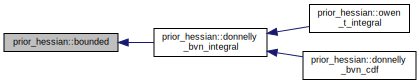
\includegraphics[width=350pt]{namespaceprior__hessian_a860bd0a9eccd25bccf6e1c002022052f_icgraph}
\end{center}
\end{figure}


\index{prior\+\_\+hessian@{prior\+\_\+hessian}!donnelly\+\_\+bvn\+\_\+cdf@{donnelly\+\_\+bvn\+\_\+cdf}}
\index{donnelly\+\_\+bvn\+\_\+cdf@{donnelly\+\_\+bvn\+\_\+cdf}!prior\+\_\+hessian@{prior\+\_\+hessian}}
\paragraph[{\texorpdfstring{donnelly\+\_\+bvn\+\_\+cdf(const Vec \&b, const Mat \&sigma)}{donnelly_bvn_cdf(const Vec &b, const Mat &sigma)}}]{\setlength{\rightskip}{0pt plus 5cm}template$<$class Vec , class Mat $>$ double prior\+\_\+hessian\+::donnelly\+\_\+bvn\+\_\+cdf (
\begin{DoxyParamCaption}
\item[{const Vec \&}]{b, }
\item[{const Mat \&}]{sigma}
\end{DoxyParamCaption}
)}\hypertarget{namespaceprior__hessian_a0f8b4ec070533193c3f402bbcc2b8b2b}{}\label{namespaceprior__hessian_a0f8b4ec070533193c3f402bbcc2b8b2b}


Definition at line 55 of file mvn\+\_\+cdf.\+h.



References donnelly\+\_\+bvn\+\_\+integral().



Here is the call graph for this function\+:\nopagebreak
\begin{figure}[H]
\begin{center}
\leavevmode
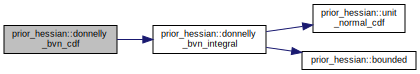
\includegraphics[width=350pt]{namespaceprior__hessian_a0f8b4ec070533193c3f402bbcc2b8b2b_cgraph}
\end{center}
\end{figure}


\index{prior\+\_\+hessian@{prior\+\_\+hessian}!donnelly\+\_\+bvn\+\_\+integral@{donnelly\+\_\+bvn\+\_\+integral}}
\index{donnelly\+\_\+bvn\+\_\+integral@{donnelly\+\_\+bvn\+\_\+integral}!prior\+\_\+hessian@{prior\+\_\+hessian}}
\paragraph[{\texorpdfstring{donnelly\+\_\+bvn\+\_\+integral(double ah, double ak, double r)}{donnelly_bvn_integral(double ah, double ak, double r)}}]{\setlength{\rightskip}{0pt plus 5cm}double prior\+\_\+hessian\+::donnelly\+\_\+bvn\+\_\+integral (
\begin{DoxyParamCaption}
\item[{double}]{ah, }
\item[{double}]{ak, }
\item[{double}]{r}
\end{DoxyParamCaption}
)}\hypertarget{namespaceprior__hessian_ae87209106163a600fbde211815f83b5a}{}\label{namespaceprior__hessian_ae87209106163a600fbde211815f83b5a}
compute the bivariate normal cdf integral computes the probability for two normal variates X and Y whose correlation is R, that AH $<$= X and AK $<$= Y.

Adapted to modern C++ with efficiency improvements by\+: Mark Olah (\href{mailto:mjo@cs.unm}{\tt mjo@cs.\+unm} D\+OT edu) 10/2018

Reference\+: Thomas Donnelly, Algorithm 462\+: Bivariate Normal Distribution, Communications of the A\+CM, October 1973, Volume 16, Number 10, page 638.

compute the upper-\/right tail of the bivariate normal distribution computes the probability for two normal variates X and Y whose correlation is R, that AH $<$= X and AK $<$= Y.

Adapted to modern C++ with efficiency improvements by\+: Mark Olah (\href{mailto:mjo@cs.unm}{\tt mjo@cs.\+unm} D\+OT edu) 10/2018

Reference\+: Thomas Donnelly, Algorithm 462\+: Bivariate Normal Distribution, Communications of the A\+CM, October 1973, Volume 16, Number 10, page 638. 

Definition at line 158 of file mvn\+\_\+cdf.\+cpp.



References bounded(), and unit\+\_\+normal\+\_\+cdf().



Referenced by donnelly\+\_\+bvn\+\_\+cdf(), and owen\+\_\+t\+\_\+integral().



Here is the call graph for this function\+:\nopagebreak
\begin{figure}[H]
\begin{center}
\leavevmode
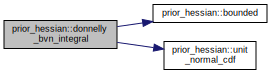
\includegraphics[width=343pt]{namespaceprior__hessian_ae87209106163a600fbde211815f83b5a_cgraph}
\end{center}
\end{figure}




Here is the caller graph for this function\+:\nopagebreak
\begin{figure}[H]
\begin{center}
\leavevmode
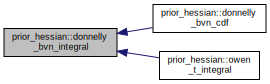
\includegraphics[width=342pt]{namespaceprior__hessian_ae87209106163a600fbde211815f83b5a_icgraph}
\end{center}
\end{figure}


\index{prior\+\_\+hessian@{prior\+\_\+hessian}!donnelly\+\_\+bvn\+\_\+integral\+\_\+orig@{donnelly\+\_\+bvn\+\_\+integral\+\_\+orig}}
\index{donnelly\+\_\+bvn\+\_\+integral\+\_\+orig@{donnelly\+\_\+bvn\+\_\+integral\+\_\+orig}!prior\+\_\+hessian@{prior\+\_\+hessian}}
\paragraph[{\texorpdfstring{donnelly\+\_\+bvn\+\_\+integral\+\_\+orig(double ah, double ak, double r)}{donnelly_bvn_integral_orig(double ah, double ak, double r)}}]{\setlength{\rightskip}{0pt plus 5cm}double prior\+\_\+hessian\+::donnelly\+\_\+bvn\+\_\+integral\+\_\+orig (
\begin{DoxyParamCaption}
\item[{double}]{ah, }
\item[{double}]{ak, }
\item[{double}]{r}
\end{DoxyParamCaption}
)}\hypertarget{namespaceprior__hessian_a4479c56bffd52c8f08515da580030958}{}\label{namespaceprior__hessian_a4479c56bffd52c8f08515da580030958}


Definition at line 268 of file mvn\+\_\+cdf.\+cpp.



References unit\+\_\+normal\+\_\+cdf().



Referenced by owen\+\_\+t\+\_\+integral().



Here is the call graph for this function\+:\nopagebreak
\begin{figure}[H]
\begin{center}
\leavevmode
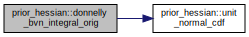
\includegraphics[width=321pt]{namespaceprior__hessian_a4479c56bffd52c8f08515da580030958_cgraph}
\end{center}
\end{figure}




Here is the caller graph for this function\+:\nopagebreak
\begin{figure}[H]
\begin{center}
\leavevmode
\includegraphics[width=329pt]{namespaceprior__hessian_a4479c56bffd52c8f08515da580030958_icgraph}
\end{center}
\end{figure}


\index{prior\+\_\+hessian@{prior\+\_\+hessian}!eulerian\+\_\+polynomial@{eulerian\+\_\+polynomial}}
\index{eulerian\+\_\+polynomial@{eulerian\+\_\+polynomial}!prior\+\_\+hessian@{prior\+\_\+hessian}}
\paragraph[{\texorpdfstring{eulerian\+\_\+polynomial()}{eulerian_polynomial()}}]{\setlength{\rightskip}{0pt plus 5cm}template$<$long N$>$ {\bf VecT} prior\+\_\+hessian\+::eulerian\+\_\+polynomial (
\begin{DoxyParamCaption}
{}
\end{DoxyParamCaption}
)}\hypertarget{namespaceprior__hessian_a05bb4a53732758396a2dc1125da71df5}{}\label{namespaceprior__hessian_a05bb4a53732758396a2dc1125da71df5}


Definition at line 33 of file Eulerian\+Polynomial.\+h.

\index{prior\+\_\+hessian@{prior\+\_\+hessian}!make\+\_\+adapted\+\_\+bounded\+\_\+dist@{make\+\_\+adapted\+\_\+bounded\+\_\+dist}}
\index{make\+\_\+adapted\+\_\+bounded\+\_\+dist@{make\+\_\+adapted\+\_\+bounded\+\_\+dist}!prior\+\_\+hessian@{prior\+\_\+hessian}}
\paragraph[{\texorpdfstring{make\+\_\+adapted\+\_\+bounded\+\_\+dist(\+Dist \&\&dist)}{make_adapted_bounded_dist(Dist &&dist)}}]{\setlength{\rightskip}{0pt plus 5cm}template$<$class Dist , typename  = meta\+::\+Enable\+If\+Is\+Not\+Tuple\+T$<$\+Dist$>$$>$ std\+::enable\+\_\+if\+\_\+t$<$ {\bf detail\+::\+Dist\+TraitsT}$<$Dist$>$\+::adaptable\+\_\+bounds, Dist$>$ prior\+\_\+hessian\+::make\+\_\+adapted\+\_\+bounded\+\_\+dist (
\begin{DoxyParamCaption}
\item[{Dist \&\&}]{dist}
\end{DoxyParamCaption}
)}\hypertarget{namespaceprior__hessian_a387cc711a6a39924943b5b20ae76bf6a}{}\label{namespaceprior__hessian_a387cc711a6a39924943b5b20ae76bf6a}
\hyperlink{namespaceprior__hessian_a387cc711a6a39924943b5b20ae76bf6a}{make\+\_\+adapted\+\_\+bounded\+\_\+dist()} \mbox{[}4-\/forms\mbox{]} If the given distribution is not bounded then the appropriate bounding distribution is wrapped around it. We detect the boundedness of the distribution using detail\+::adaptable\+\_\+bounds type-\/traits class. Can be replaced with constexpr if in c++17. Uses S\+F\+I\+N\+AE in c++14. 

Definition at line 99 of file Bounds\+Adapted\+Dist.\+h.



Referenced by prior\+\_\+hessian\+::detail\+::make\+\_\+adapted\+\_\+bounded\+\_\+dist\+\_\+tuple(), make\+\_\+adapted\+\_\+bounded\+\_\+dist\+\_\+tuple(), prior\+\_\+hessian\+::\+Composite\+Dist\+::make\+\_\+component\+\_\+dist(), prior\+\_\+hessian\+::\+Composite\+Dist\+::make\+\_\+component\+\_\+dist\+\_\+tuple(), and make\+\_\+copula\+\_\+dist().



Here is the caller graph for this function\+:\nopagebreak
\begin{figure}[H]
\begin{center}
\leavevmode
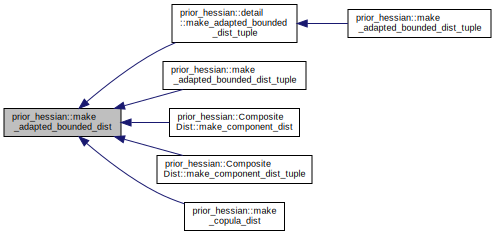
\includegraphics[width=350pt]{namespaceprior__hessian_a387cc711a6a39924943b5b20ae76bf6a_icgraph}
\end{center}
\end{figure}


\index{prior\+\_\+hessian@{prior\+\_\+hessian}!make\+\_\+adapted\+\_\+bounded\+\_\+dist@{make\+\_\+adapted\+\_\+bounded\+\_\+dist}}
\index{make\+\_\+adapted\+\_\+bounded\+\_\+dist@{make\+\_\+adapted\+\_\+bounded\+\_\+dist}!prior\+\_\+hessian@{prior\+\_\+hessian}}
\paragraph[{\texorpdfstring{make\+\_\+adapted\+\_\+bounded\+\_\+dist(\+Dist \&\&dist)}{make_adapted_bounded_dist(Dist &&dist)}}]{\setlength{\rightskip}{0pt plus 5cm}template$<$class Dist , typename  = meta\+::\+Enable\+If\+Is\+Not\+Tuple\+T$<$\+Dist$>$$>$ std\+::enable\+\_\+if\+\_\+t$<$ !{\bf detail\+::\+Dist\+TraitsT}$<$Dist$>$\+::adaptable\+\_\+bounds, {\bf Bounds\+Adapted\+DistT}$<$Dist$>$ $>$ prior\+\_\+hessian\+::make\+\_\+adapted\+\_\+bounded\+\_\+dist (
\begin{DoxyParamCaption}
\item[{Dist \&\&}]{dist}
\end{DoxyParamCaption}
)}\hypertarget{namespaceprior__hessian_aac9684eb25c8e9eb2b10640931a08285}{}\label{namespaceprior__hessian_aac9684eb25c8e9eb2b10640931a08285}


Definition at line 104 of file Bounds\+Adapted\+Dist.\+h.

\index{prior\+\_\+hessian@{prior\+\_\+hessian}!make\+\_\+adapted\+\_\+bounded\+\_\+dist@{make\+\_\+adapted\+\_\+bounded\+\_\+dist}}
\index{make\+\_\+adapted\+\_\+bounded\+\_\+dist@{make\+\_\+adapted\+\_\+bounded\+\_\+dist}!prior\+\_\+hessian@{prior\+\_\+hessian}}
\paragraph[{\texorpdfstring{make\+\_\+adapted\+\_\+bounded\+\_\+dist(\+Dist \&\&dist, Vec \&\&lbound, Vec \&\&ubound)}{make_adapted_bounded_dist(Dist &&dist, Vec &&lbound, Vec &&ubound)}}]{\setlength{\rightskip}{0pt plus 5cm}template$<$class Dist , class Vec , typename  = meta\+::\+Enable\+If\+Is\+Not\+Tuple\+T$<$\+Dist$>$$>$ std\+::enable\+\_\+if\+\_\+t$<${\bf detail\+::\+Dist\+TraitsT}$<$Dist$>$\+::adaptable\+\_\+bounds, Dist$>$ prior\+\_\+hessian\+::make\+\_\+adapted\+\_\+bounded\+\_\+dist (
\begin{DoxyParamCaption}
\item[{Dist \&\&}]{dist, }
\item[{Vec \&\&}]{lbound, }
\item[{Vec \&\&}]{ubound}
\end{DoxyParamCaption}
)}\hypertarget{namespaceprior__hessian_ace3ed32ae08101fa6cddfb56cc39f3a9}{}\label{namespaceprior__hessian_ace3ed32ae08101fa6cddfb56cc39f3a9}


Definition at line 109 of file Bounds\+Adapted\+Dist.\+h.

\index{prior\+\_\+hessian@{prior\+\_\+hessian}!make\+\_\+adapted\+\_\+bounded\+\_\+dist@{make\+\_\+adapted\+\_\+bounded\+\_\+dist}}
\index{make\+\_\+adapted\+\_\+bounded\+\_\+dist@{make\+\_\+adapted\+\_\+bounded\+\_\+dist}!prior\+\_\+hessian@{prior\+\_\+hessian}}
\paragraph[{\texorpdfstring{make\+\_\+adapted\+\_\+bounded\+\_\+dist(\+Dist \&\&dist, Vec \&\&lbound, Vec \&\&ubound)}{make_adapted_bounded_dist(Dist &&dist, Vec &&lbound, Vec &&ubound)}}]{\setlength{\rightskip}{0pt plus 5cm}template$<$class Dist , class Vec , typename  = meta\+::\+Enable\+If\+Is\+Not\+Tuple\+T$<$\+Dist$>$$>$ std\+::enable\+\_\+if\+\_\+t$<$!{\bf detail\+::\+Dist\+TraitsT}$<$Dist$>$\+::adaptable\+\_\+bounds, {\bf Bounds\+Adapted\+DistT}$<$Dist$>$ $>$ prior\+\_\+hessian\+::make\+\_\+adapted\+\_\+bounded\+\_\+dist (
\begin{DoxyParamCaption}
\item[{Dist \&\&}]{dist, }
\item[{Vec \&\&}]{lbound, }
\item[{Vec \&\&}]{ubound}
\end{DoxyParamCaption}
)}\hypertarget{namespaceprior__hessian_ab331d08c528526111610cf1407ca43c1}{}\label{namespaceprior__hessian_ab331d08c528526111610cf1407ca43c1}


Definition at line 117 of file Bounds\+Adapted\+Dist.\+h.

\index{prior\+\_\+hessian@{prior\+\_\+hessian}!make\+\_\+adapted\+\_\+bounded\+\_\+dist\+\_\+tuple@{make\+\_\+adapted\+\_\+bounded\+\_\+dist\+\_\+tuple}}
\index{make\+\_\+adapted\+\_\+bounded\+\_\+dist\+\_\+tuple@{make\+\_\+adapted\+\_\+bounded\+\_\+dist\+\_\+tuple}!prior\+\_\+hessian@{prior\+\_\+hessian}}
\paragraph[{\texorpdfstring{make\+\_\+adapted\+\_\+bounded\+\_\+dist\+\_\+tuple(\+Ts \&\&...\+ts)}{make_adapted_bounded_dist_tuple(Ts &&...ts)}}]{\setlength{\rightskip}{0pt plus 5cm}template$<$class... Ts$>$ std\+::tuple$<${\bf Bounds\+Adapted\+DistT}$<$Ts$>$...$>$ prior\+\_\+hessian\+::make\+\_\+adapted\+\_\+bounded\+\_\+dist\+\_\+tuple (
\begin{DoxyParamCaption}
\item[{Ts \&\&...}]{ts}
\end{DoxyParamCaption}
)}\hypertarget{namespaceprior__hessian_a55f558964ebfac8734141e232a376bb7}{}\label{namespaceprior__hessian_a55f558964ebfac8734141e232a376bb7}


Definition at line 132 of file Bounds\+Adapted\+Dist.\+h.



References make\+\_\+adapted\+\_\+bounded\+\_\+dist().



Here is the call graph for this function\+:\nopagebreak
\begin{figure}[H]
\begin{center}
\leavevmode
\includegraphics[width=350pt]{namespaceprior__hessian_a55f558964ebfac8734141e232a376bb7_cgraph}
\end{center}
\end{figure}


\index{prior\+\_\+hessian@{prior\+\_\+hessian}!make\+\_\+adapted\+\_\+bounded\+\_\+dist\+\_\+tuple@{make\+\_\+adapted\+\_\+bounded\+\_\+dist\+\_\+tuple}}
\index{make\+\_\+adapted\+\_\+bounded\+\_\+dist\+\_\+tuple@{make\+\_\+adapted\+\_\+bounded\+\_\+dist\+\_\+tuple}!prior\+\_\+hessian@{prior\+\_\+hessian}}
\paragraph[{\texorpdfstring{make\+\_\+adapted\+\_\+bounded\+\_\+dist\+\_\+tuple(std\+::tuple$<$ Ts... $>$ \&\&dists)}{make_adapted_bounded_dist_tuple(std::tuple< Ts... > &&dists)}}]{\setlength{\rightskip}{0pt plus 5cm}template$<$class... Ts$>$ std\+::tuple$<${\bf Bounds\+Adapted\+DistT}$<$Ts$>$...$>$ prior\+\_\+hessian\+::make\+\_\+adapted\+\_\+bounded\+\_\+dist\+\_\+tuple (
\begin{DoxyParamCaption}
\item[{std\+::tuple$<$ Ts... $>$ \&\&}]{dists}
\end{DoxyParamCaption}
)}\hypertarget{namespaceprior__hessian_a95fddb21432915b6b47579b4ad05602f}{}\label{namespaceprior__hessian_a95fddb21432915b6b47579b4ad05602f}


Definition at line 139 of file Bounds\+Adapted\+Dist.\+h.



References prior\+\_\+hessian\+::detail\+::make\+\_\+adapted\+\_\+bounded\+\_\+dist\+\_\+tuple().



Here is the call graph for this function\+:\nopagebreak
\begin{figure}[H]
\begin{center}
\leavevmode
\includegraphics[width=350pt]{namespaceprior__hessian_a95fddb21432915b6b47579b4ad05602f_cgraph}
\end{center}
\end{figure}


\index{prior\+\_\+hessian@{prior\+\_\+hessian}!make\+\_\+adapted\+\_\+bounded\+\_\+dist\+\_\+tuple@{make\+\_\+adapted\+\_\+bounded\+\_\+dist\+\_\+tuple}}
\index{make\+\_\+adapted\+\_\+bounded\+\_\+dist\+\_\+tuple@{make\+\_\+adapted\+\_\+bounded\+\_\+dist\+\_\+tuple}!prior\+\_\+hessian@{prior\+\_\+hessian}}
\paragraph[{\texorpdfstring{make\+\_\+adapted\+\_\+bounded\+\_\+dist\+\_\+tuple(const std\+::tuple$<$ Ts... $>$ \&dists)}{make_adapted_bounded_dist_tuple(const std::tuple< Ts... > &dists)}}]{\setlength{\rightskip}{0pt plus 5cm}template$<$class... Ts$>$ std\+::tuple$<${\bf Bounds\+Adapted\+DistT}$<$Ts$>$...$>$ prior\+\_\+hessian\+::make\+\_\+adapted\+\_\+bounded\+\_\+dist\+\_\+tuple (
\begin{DoxyParamCaption}
\item[{const std\+::tuple$<$ Ts... $>$ \&}]{dists}
\end{DoxyParamCaption}
)}\hypertarget{namespaceprior__hessian_a277a764f9d5df7ff208e9052de05f067}{}\label{namespaceprior__hessian_a277a764f9d5df7ff208e9052de05f067}


Definition at line 146 of file Bounds\+Adapted\+Dist.\+h.



References prior\+\_\+hessian\+::detail\+::make\+\_\+adapted\+\_\+bounded\+\_\+dist\+\_\+tuple().



Here is the call graph for this function\+:\nopagebreak
\begin{figure}[H]
\begin{center}
\leavevmode
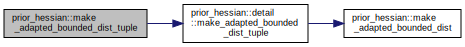
\includegraphics[width=350pt]{namespaceprior__hessian_a277a764f9d5df7ff208e9052de05f067_cgraph}
\end{center}
\end{figure}


\index{prior\+\_\+hessian@{prior\+\_\+hessian}!make\+\_\+bounded\+\_\+gamma\+\_\+dist@{make\+\_\+bounded\+\_\+gamma\+\_\+dist}}
\index{make\+\_\+bounded\+\_\+gamma\+\_\+dist@{make\+\_\+bounded\+\_\+gamma\+\_\+dist}!prior\+\_\+hessian@{prior\+\_\+hessian}}
\paragraph[{\texorpdfstring{make\+\_\+bounded\+\_\+gamma\+\_\+dist(double scale, double shape, std\+::pair$<$ double, double $>$ bounds)}{make_bounded_gamma_dist(double scale, double shape, std::pair< double, double > bounds)}}]{\setlength{\rightskip}{0pt plus 5cm}{\bf Truncated\+Gamma\+Dist} prior\+\_\+hessian\+::make\+\_\+bounded\+\_\+gamma\+\_\+dist (
\begin{DoxyParamCaption}
\item[{double}]{scale, }
\item[{double}]{shape, }
\item[{std\+::pair$<$ double, double $>$}]{bounds}
\end{DoxyParamCaption}
)\hspace{0.3cm}{\ttfamily [inline]}}\hypertarget{namespaceprior__hessian_abd1783a43cab6f6855e54eb1faab39d4}{}\label{namespaceprior__hessian_abd1783a43cab6f6855e54eb1faab39d4}


Definition at line 18 of file Truncated\+Gamma\+Dist.\+h.

\index{prior\+\_\+hessian@{prior\+\_\+hessian}!make\+\_\+bounded\+\_\+multivariate\+\_\+normal\+\_\+dist@{make\+\_\+bounded\+\_\+multivariate\+\_\+normal\+\_\+dist}}
\index{make\+\_\+bounded\+\_\+multivariate\+\_\+normal\+\_\+dist@{make\+\_\+bounded\+\_\+multivariate\+\_\+normal\+\_\+dist}!prior\+\_\+hessian@{prior\+\_\+hessian}}
\paragraph[{\texorpdfstring{make\+\_\+bounded\+\_\+multivariate\+\_\+normal\+\_\+dist(\+Vec \&\&mu, Mat \&\&sigma, Vec2 \&\&lbound, Vec2 \&\&ubound)}{make_bounded_multivariate_normal_dist(Vec &&mu, Mat &&sigma, Vec2 &&lbound, Vec2 &&ubound)}}]{\setlength{\rightskip}{0pt plus 5cm}template$<$IdxT Ndim, class Vec , class Mat , class Vec2 $>$ {\bf Truncated\+Multivariate\+Normal\+Dist}$<$Ndim$>$ prior\+\_\+hessian\+::make\+\_\+bounded\+\_\+multivariate\+\_\+normal\+\_\+dist (
\begin{DoxyParamCaption}
\item[{Vec \&\&}]{mu, }
\item[{Mat \&\&}]{sigma, }
\item[{Vec2 \&\&}]{lbound, }
\item[{Vec2 \&\&}]{ubound}
\end{DoxyParamCaption}
)}\hypertarget{namespaceprior__hessian_a51a85cfe6ac613ed9b703e10280c1bbb}{}\label{namespaceprior__hessian_a51a85cfe6ac613ed9b703e10280c1bbb}


Definition at line 22 of file Truncated\+Multivariate\+Normal\+Dist.\+h.

\index{prior\+\_\+hessian@{prior\+\_\+hessian}!make\+\_\+bounded\+\_\+normal\+\_\+dist@{make\+\_\+bounded\+\_\+normal\+\_\+dist}}
\index{make\+\_\+bounded\+\_\+normal\+\_\+dist@{make\+\_\+bounded\+\_\+normal\+\_\+dist}!prior\+\_\+hessian@{prior\+\_\+hessian}}
\paragraph[{\texorpdfstring{make\+\_\+bounded\+\_\+normal\+\_\+dist(double mu, double sigma, std\+::pair$<$ double, double $>$ bounds)}{make_bounded_normal_dist(double mu, double sigma, std::pair< double, double > bounds)}}]{\setlength{\rightskip}{0pt plus 5cm}{\bf Truncated\+Normal\+Dist} prior\+\_\+hessian\+::make\+\_\+bounded\+\_\+normal\+\_\+dist (
\begin{DoxyParamCaption}
\item[{double}]{mu, }
\item[{double}]{sigma, }
\item[{std\+::pair$<$ double, double $>$}]{bounds}
\end{DoxyParamCaption}
)\hspace{0.3cm}{\ttfamily [inline]}}\hypertarget{namespaceprior__hessian_a14ebf8db869f2c1e45781e41e69b3420}{}\label{namespaceprior__hessian_a14ebf8db869f2c1e45781e41e69b3420}


Definition at line 20 of file Truncated\+Normal\+Dist.\+h.

\index{prior\+\_\+hessian@{prior\+\_\+hessian}!make\+\_\+bounded\+\_\+pareto\+\_\+dist@{make\+\_\+bounded\+\_\+pareto\+\_\+dist}}
\index{make\+\_\+bounded\+\_\+pareto\+\_\+dist@{make\+\_\+bounded\+\_\+pareto\+\_\+dist}!prior\+\_\+hessian@{prior\+\_\+hessian}}
\paragraph[{\texorpdfstring{make\+\_\+bounded\+\_\+pareto\+\_\+dist(double alpha, std\+::pair$<$ double, double $>$ bounds)}{make_bounded_pareto_dist(double alpha, std::pair< double, double > bounds)}}]{\setlength{\rightskip}{0pt plus 5cm}{\bf Truncated\+Pareto\+Dist} prior\+\_\+hessian\+::make\+\_\+bounded\+\_\+pareto\+\_\+dist (
\begin{DoxyParamCaption}
\item[{double}]{alpha, }
\item[{std\+::pair$<$ double, double $>$}]{bounds}
\end{DoxyParamCaption}
)\hspace{0.3cm}{\ttfamily [inline]}}\hypertarget{namespaceprior__hessian_ae6d920b436127ce4698e75575581eed5}{}\label{namespaceprior__hessian_ae6d920b436127ce4698e75575581eed5}


Definition at line 18 of file Truncated\+Pareto\+Dist.\+h.

\index{prior\+\_\+hessian@{prior\+\_\+hessian}!make\+\_\+copula\+\_\+dist@{make\+\_\+copula\+\_\+dist}}
\index{make\+\_\+copula\+\_\+dist@{make\+\_\+copula\+\_\+dist}!prior\+\_\+hessian@{prior\+\_\+hessian}}
\paragraph[{\texorpdfstring{make\+\_\+copula\+\_\+dist(\+Copula\+Template$<$ sizeof...(\+Marginal\+Dist\+Ts)$>$ \&\&copula, Marginal\+Dist\+Ts \&\&...\+dists)}{make_copula_dist(CopulaTemplate< sizeof...(MarginalDistTs)> &&copula, MarginalDistTs &&...dists)}}]{\setlength{\rightskip}{0pt plus 5cm}template$<$template$<$ int $>$ class Copula\+Template, class... Marginal\+Dist\+Ts$>$ {\bf Copula\+Dist}$<$Copula\+Template,Marginal\+Dist\+Ts...$>$ prior\+\_\+hessian\+::make\+\_\+copula\+\_\+dist (
\begin{DoxyParamCaption}
\item[{Copula\+Template$<$ sizeof...(Marginal\+Dist\+Ts)$>$ \&\&}]{copula, }
\item[{Marginal\+Dist\+Ts \&\&...}]{dists}
\end{DoxyParamCaption}
)}\hypertarget{namespaceprior__hessian_a0cfb582e76e0bbae3498707a8458cb78}{}\label{namespaceprior__hessian_a0cfb582e76e0bbae3498707a8458cb78}


Definition at line 187 of file Copula\+Dist.\+h.



References make\+\_\+adapted\+\_\+bounded\+\_\+dist().



Here is the call graph for this function\+:\nopagebreak
\begin{figure}[H]
\begin{center}
\leavevmode
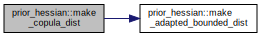
\includegraphics[width=333pt]{namespaceprior__hessian_a0cfb582e76e0bbae3498707a8458cb78_cgraph}
\end{center}
\end{figure}


\index{prior\+\_\+hessian@{prior\+\_\+hessian}!make\+\_\+scaled\+\_\+symmetric\+\_\+beta\+\_\+dist@{make\+\_\+scaled\+\_\+symmetric\+\_\+beta\+\_\+dist}}
\index{make\+\_\+scaled\+\_\+symmetric\+\_\+beta\+\_\+dist@{make\+\_\+scaled\+\_\+symmetric\+\_\+beta\+\_\+dist}!prior\+\_\+hessian@{prior\+\_\+hessian}}
\paragraph[{\texorpdfstring{make\+\_\+scaled\+\_\+symmetric\+\_\+beta\+\_\+dist(double beta, std\+::pair$<$ double, double $>$ bounds)}{make_scaled_symmetric_beta_dist(double beta, std::pair< double, double > bounds)}}]{\setlength{\rightskip}{0pt plus 5cm}{\bf Scaled\+Symmetric\+Beta\+Dist} prior\+\_\+hessian\+::make\+\_\+scaled\+\_\+symmetric\+\_\+beta\+\_\+dist (
\begin{DoxyParamCaption}
\item[{double}]{beta, }
\item[{std\+::pair$<$ double, double $>$}]{bounds}
\end{DoxyParamCaption}
)\hspace{0.3cm}{\ttfamily [inline]}}\hypertarget{namespaceprior__hessian_a2dd8c3c31f349117f96fdddc94d54dd8}{}\label{namespaceprior__hessian_a2dd8c3c31f349117f96fdddc94d54dd8}


Definition at line 18 of file Scaled\+Symmetric\+Beta\+Dist.\+h.

\index{prior\+\_\+hessian@{prior\+\_\+hessian}!mc\+\_\+mvn\+\_\+cdf@{mc\+\_\+mvn\+\_\+cdf}}
\index{mc\+\_\+mvn\+\_\+cdf@{mc\+\_\+mvn\+\_\+cdf}!prior\+\_\+hessian@{prior\+\_\+hessian}}
\paragraph[{\texorpdfstring{mc\+\_\+mvn\+\_\+cdf(const Vec \&b, const Mat \&\+S, double \&error)}{mc_mvn_cdf(const Vec &b, const Mat &S, double &error)}}]{\setlength{\rightskip}{0pt plus 5cm}template$<$class Vec , class Mat $>$ double prior\+\_\+hessian\+::mc\+\_\+mvn\+\_\+cdf (
\begin{DoxyParamCaption}
\item[{const Vec \&}]{b, }
\item[{const Mat \&}]{S, }
\item[{double \&}]{error}
\end{DoxyParamCaption}
)}\hypertarget{namespaceprior__hessian_a923402e085c726e416b02817a6d47337}{}\label{namespaceprior__hessian_a923402e085c726e416b02817a6d47337}


Definition at line 169 of file mvn\+\_\+cdf.\+h.



References mc\+\_\+mvn\+\_\+cdf\+\_\+core().



Here is the call graph for this function\+:\nopagebreak
\begin{figure}[H]
\begin{center}
\leavevmode
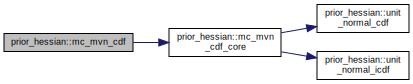
\includegraphics[width=350pt]{namespaceprior__hessian_a923402e085c726e416b02817a6d47337_cgraph}
\end{center}
\end{figure}


\index{prior\+\_\+hessian@{prior\+\_\+hessian}!mc\+\_\+mvn\+\_\+cdf\+\_\+core@{mc\+\_\+mvn\+\_\+cdf\+\_\+core}}
\index{mc\+\_\+mvn\+\_\+cdf\+\_\+core@{mc\+\_\+mvn\+\_\+cdf\+\_\+core}!prior\+\_\+hessian@{prior\+\_\+hessian}}
\paragraph[{\texorpdfstring{mc\+\_\+mvn\+\_\+cdf\+\_\+core(const Vec \&b, const Mat \&\+U, double \&error, int \&niter)}{mc_mvn_cdf_core(const Vec &b, const Mat &U, double &error, int &niter)}}]{\setlength{\rightskip}{0pt plus 5cm}template$<$class Vec , class Mat $>$ double prior\+\_\+hessian\+::mc\+\_\+mvn\+\_\+cdf\+\_\+core (
\begin{DoxyParamCaption}
\item[{const Vec \&}]{b, }
\item[{const Mat \&}]{U, }
\item[{double \&}]{error, }
\item[{int \&}]{niter}
\end{DoxyParamCaption}
)}\hypertarget{namespaceprior__hessian_af30ccf313fd6eced8ae174f6a0d8457b}{}\label{namespaceprior__hessian_af30ccf313fd6eced8ae174f6a0d8457b}
For the cdf a=-\/\+Infinity, so d=0. 

Definition at line 130 of file mvn\+\_\+cdf.\+h.



References unit\+\_\+normal\+\_\+cdf(), and unit\+\_\+normal\+\_\+icdf().



Referenced by mc\+\_\+mvn\+\_\+cdf().



Here is the call graph for this function\+:\nopagebreak
\begin{figure}[H]
\begin{center}
\leavevmode
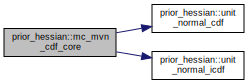
\includegraphics[width=320pt]{namespaceprior__hessian_af30ccf313fd6eced8ae174f6a0d8457b_cgraph}
\end{center}
\end{figure}




Here is the caller graph for this function\+:\nopagebreak
\begin{figure}[H]
\begin{center}
\leavevmode
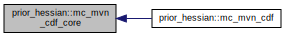
\includegraphics[width=350pt]{namespaceprior__hessian_af30ccf313fd6eced8ae174f6a0d8457b_icgraph}
\end{center}
\end{figure}


\index{prior\+\_\+hessian@{prior\+\_\+hessian}!mc\+\_\+mvn\+\_\+integral@{mc\+\_\+mvn\+\_\+integral}}
\index{mc\+\_\+mvn\+\_\+integral@{mc\+\_\+mvn\+\_\+integral}!prior\+\_\+hessian@{prior\+\_\+hessian}}
\paragraph[{\texorpdfstring{mc\+\_\+mvn\+\_\+integral(const Vec \&a, const Vec \&b, const Mat \&\+U, double \&error, int \&niter)}{mc_mvn_integral(const Vec &a, const Vec &b, const Mat &U, double &error, int &niter)}}]{\setlength{\rightskip}{0pt plus 5cm}template$<$class Vec , class Mat $>$ double prior\+\_\+hessian\+::mc\+\_\+mvn\+\_\+integral (
\begin{DoxyParamCaption}
\item[{const Vec \&}]{a, }
\item[{const Vec \&}]{b, }
\item[{const Mat \&}]{U, }
\item[{double \&}]{error, }
\item[{int \&}]{niter}
\end{DoxyParamCaption}
)}\hypertarget{namespaceprior__hessian_abadcc969aeb37b0c2f1e69c75731ec65}{}\label{namespaceprior__hessian_abadcc969aeb37b0c2f1e69c75731ec65}
compute the multivariate normal cdf integral 

Definition at line 81 of file mvn\+\_\+cdf.\+h.



References unit\+\_\+normal\+\_\+cdf(), and unit\+\_\+normal\+\_\+icdf().



Here is the call graph for this function\+:\nopagebreak
\begin{figure}[H]
\begin{center}
\leavevmode
\includegraphics[width=320pt]{namespaceprior__hessian_abadcc969aeb37b0c2f1e69c75731ec65_cgraph}
\end{center}
\end{figure}


\index{prior\+\_\+hessian@{prior\+\_\+hessian}!operator$<$$<$@{operator$<$$<$}}
\index{operator$<$$<$@{operator$<$$<$}!prior\+\_\+hessian@{prior\+\_\+hessian}}
\paragraph[{\texorpdfstring{operator$<$$<$(std\+::ostream \&out, const Composite\+Dist \&comp\+\_\+dist)}{operator<<(std::ostream &out, const CompositeDist &comp_dist)}}]{\setlength{\rightskip}{0pt plus 5cm}std\+::ostream \& prior\+\_\+hessian\+::operator$<$$<$ (
\begin{DoxyParamCaption}
\item[{std\+::ostream \&}]{out, }
\item[{const {\bf Composite\+Dist} \&}]{comp\+\_\+dist}
\end{DoxyParamCaption}
)}\hypertarget{namespaceprior__hessian_ab26e9ddc3b6a5caccf5d75e1a1e1af1b}{}\label{namespaceprior__hessian_ab26e9ddc3b6a5caccf5d75e1a1e1af1b}


Definition at line 80 of file Composite\+Dist.\+cpp.



References prior\+\_\+hessian\+::\+Composite\+Dist\+::component\+\_\+names(), prior\+\_\+hessian\+::\+Composite\+Dist\+::dim\+\_\+variables(), prior\+\_\+hessian\+::\+Composite\+Dist\+::global\+\_\+lbound(), prior\+\_\+hessian\+::\+Composite\+Dist\+::global\+\_\+ubound(), prior\+\_\+hessian\+::\+Composite\+Dist\+::lbound(), prior\+\_\+hessian\+::\+Composite\+Dist\+::num\+\_\+components(), prior\+\_\+hessian\+::\+Composite\+Dist\+::num\+\_\+dim(), prior\+\_\+hessian\+::\+Composite\+Dist\+::num\+\_\+dim\+\_\+components(), prior\+\_\+hessian\+::\+Composite\+Dist\+::num\+\_\+params(), prior\+\_\+hessian\+::\+Composite\+Dist\+::num\+\_\+params\+\_\+components(), prior\+\_\+hessian\+::\+Composite\+Dist\+::param\+\_\+names(), prior\+\_\+hessian\+::\+Composite\+Dist\+::params(), prior\+\_\+hessian\+::\+Composite\+Dist\+::params\+\_\+lbound(), prior\+\_\+hessian\+::\+Composite\+Dist\+::params\+\_\+ubound(), and prior\+\_\+hessian\+::\+Composite\+Dist\+::ubound().



Referenced by prior\+\_\+hessian\+::\+Composite\+Dist\+::set\+\_\+param\+\_\+names().



Here is the call graph for this function\+:\nopagebreak
\begin{figure}[H]
\begin{center}
\leavevmode
\includegraphics[width=350pt]{namespaceprior__hessian_ab26e9ddc3b6a5caccf5d75e1a1e1af1b_cgraph}
\end{center}
\end{figure}




Here is the caller graph for this function\+:\nopagebreak
\begin{figure}[H]
\begin{center}
\leavevmode
\includegraphics[width=350pt]{namespaceprior__hessian_ab26e9ddc3b6a5caccf5d75e1a1e1af1b_icgraph}
\end{center}
\end{figure}


\index{prior\+\_\+hessian@{prior\+\_\+hessian}!owen\+\_\+b\+\_\+integral@{owen\+\_\+b\+\_\+integral}}
\index{owen\+\_\+b\+\_\+integral@{owen\+\_\+b\+\_\+integral}!prior\+\_\+hessian@{prior\+\_\+hessian}}
\paragraph[{\texorpdfstring{owen\+\_\+b\+\_\+integral(double h, double k, double r)}{owen_b_integral(double h, double k, double r)}}]{\setlength{\rightskip}{0pt plus 5cm}double prior\+\_\+hessian\+::owen\+\_\+b\+\_\+integral (
\begin{DoxyParamCaption}
\item[{double}]{h, }
\item[{double}]{k, }
\item[{double}]{r}
\end{DoxyParamCaption}
)}\hypertarget{namespaceprior__hessian_a8e1226cb7a7a644fe985a8530b3df07a}{}\label{namespaceprior__hessian_a8e1226cb7a7a644fe985a8530b3df07a}


Definition at line 108 of file mvn\+\_\+cdf.\+cpp.



References owen\+\_\+t\+\_\+integral(), and unit\+\_\+normal\+\_\+cdf().



Referenced by owen\+\_\+bvn\+\_\+cdf(), and owen\+\_\+t\+\_\+integral().



Here is the call graph for this function\+:\nopagebreak
\begin{figure}[H]
\begin{center}
\leavevmode
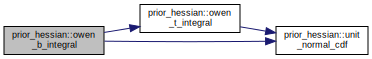
\includegraphics[width=350pt]{namespaceprior__hessian_a8e1226cb7a7a644fe985a8530b3df07a_cgraph}
\end{center}
\end{figure}




Here is the caller graph for this function\+:\nopagebreak
\begin{figure}[H]
\begin{center}
\leavevmode
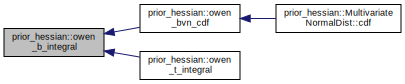
\includegraphics[width=350pt]{namespaceprior__hessian_a8e1226cb7a7a644fe985a8530b3df07a_icgraph}
\end{center}
\end{figure}


\index{prior\+\_\+hessian@{prior\+\_\+hessian}!owen\+\_\+bvn\+\_\+cdf@{owen\+\_\+bvn\+\_\+cdf}}
\index{owen\+\_\+bvn\+\_\+cdf@{owen\+\_\+bvn\+\_\+cdf}!prior\+\_\+hessian@{prior\+\_\+hessian}}
\paragraph[{\texorpdfstring{owen\+\_\+bvn\+\_\+cdf(const Vec \&b, const Mat \&sigma)}{owen_bvn_cdf(const Vec &b, const Mat &sigma)}}]{\setlength{\rightskip}{0pt plus 5cm}template$<$class Vec , class Mat $>$ double prior\+\_\+hessian\+::owen\+\_\+bvn\+\_\+cdf (
\begin{DoxyParamCaption}
\item[{const Vec \&}]{b, }
\item[{const Mat \&}]{sigma}
\end{DoxyParamCaption}
)}\hypertarget{namespaceprior__hessian_a5f7ff26e783adec5fd8ba5e290a7c892}{}\label{namespaceprior__hessian_a5f7ff26e783adec5fd8ba5e290a7c892}


Definition at line 67 of file mvn\+\_\+cdf.\+h.



References owen\+\_\+b\+\_\+integral().



Referenced by prior\+\_\+hessian\+::\+Multivariate\+Normal\+Dist$<$ Ndim $>$\+::cdf().



Here is the call graph for this function\+:\nopagebreak
\begin{figure}[H]
\begin{center}
\leavevmode
\includegraphics[width=350pt]{namespaceprior__hessian_a5f7ff26e783adec5fd8ba5e290a7c892_cgraph}
\end{center}
\end{figure}




Here is the caller graph for this function\+:\nopagebreak
\begin{figure}[H]
\begin{center}
\leavevmode
\includegraphics[width=341pt]{namespaceprior__hessian_a5f7ff26e783adec5fd8ba5e290a7c892_icgraph}
\end{center}
\end{figure}


\index{prior\+\_\+hessian@{prior\+\_\+hessian}!owen\+\_\+t\+\_\+integral@{owen\+\_\+t\+\_\+integral}}
\index{owen\+\_\+t\+\_\+integral@{owen\+\_\+t\+\_\+integral}!prior\+\_\+hessian@{prior\+\_\+hessian}}
\paragraph[{\texorpdfstring{owen\+\_\+t\+\_\+integral(double h, double a)}{owen_t_integral(double h, double a)}}]{\setlength{\rightskip}{0pt plus 5cm}double prior\+\_\+hessian\+::owen\+\_\+t\+\_\+integral (
\begin{DoxyParamCaption}
\item[{double}]{h, }
\item[{double}]{a}
\end{DoxyParamCaption}
)\hspace{0.3cm}{\ttfamily [inline]}}\hypertarget{namespaceprior__hessian_a12c3a5763e9fbc82e2fb39b8c0273cda}{}\label{namespaceprior__hessian_a12c3a5763e9fbc82e2fb39b8c0273cda}


Definition at line 26 of file mvn\+\_\+cdf.\+h.



References donnelly\+\_\+bvn\+\_\+integral(), donnelly\+\_\+bvn\+\_\+integral\+\_\+orig(), owen\+\_\+b\+\_\+integral(), owen\+\_\+t\+\_\+integral(), and unit\+\_\+normal\+\_\+cdf().



Here is the call graph for this function\+:\nopagebreak
\begin{figure}[H]
\begin{center}
\leavevmode
\includegraphics[width=350pt]{namespaceprior__hessian_a12c3a5763e9fbc82e2fb39b8c0273cda_cgraph}
\end{center}
\end{figure}


\index{prior\+\_\+hessian@{prior\+\_\+hessian}!owen\+\_\+t\+\_\+integral@{owen\+\_\+t\+\_\+integral}}
\index{owen\+\_\+t\+\_\+integral@{owen\+\_\+t\+\_\+integral}!prior\+\_\+hessian@{prior\+\_\+hessian}}
\paragraph[{\texorpdfstring{owen\+\_\+t\+\_\+integral(double h, double a, double gh)}{owen_t_integral(double h, double a, double gh)}}]{\setlength{\rightskip}{0pt plus 5cm}double prior\+\_\+hessian\+::owen\+\_\+t\+\_\+integral (
\begin{DoxyParamCaption}
\item[{double}]{h, }
\item[{double}]{a, }
\item[{double}]{gh}
\end{DoxyParamCaption}
)}\hypertarget{namespaceprior__hessian_a31c9cb28381da665bdef9a77b4858fc5}{}\label{namespaceprior__hessian_a31c9cb28381da665bdef9a77b4858fc5}


Definition at line 54 of file mvn\+\_\+cdf.\+cpp.



References unit\+\_\+normal\+\_\+cdf().



Referenced by owen\+\_\+b\+\_\+integral(), and owen\+\_\+t\+\_\+integral().



Here is the call graph for this function\+:\nopagebreak
\begin{figure}[H]
\begin{center}
\leavevmode
\includegraphics[width=308pt]{namespaceprior__hessian_a31c9cb28381da665bdef9a77b4858fc5_cgraph}
\end{center}
\end{figure}




Here is the caller graph for this function\+:\nopagebreak
\begin{figure}[H]
\begin{center}
\leavevmode
\includegraphics[width=350pt]{namespaceprior__hessian_a31c9cb28381da665bdef9a77b4858fc5_icgraph}
\end{center}
\end{figure}


\index{prior\+\_\+hessian@{prior\+\_\+hessian}!square@{square}}
\index{square@{square}!prior\+\_\+hessian@{prior\+\_\+hessian}}
\paragraph[{\texorpdfstring{square(\+T t)}{square(T t)}}]{\setlength{\rightskip}{0pt plus 5cm}template$<$class T $>$ T prior\+\_\+hessian\+::square (
\begin{DoxyParamCaption}
\item[{T}]{t}
\end{DoxyParamCaption}
)}\hypertarget{namespaceprior__hessian_a706cb136b90f16dd920118eb59ef1ad6}{}\label{namespaceprior__hessian_a706cb136b90f16dd920118eb59ef1ad6}


Definition at line 44 of file util.\+h.



Referenced by prior\+\_\+hessian\+::helpers\+::compute\+\_\+quadratic\+\_\+from\+\_\+symmetric(), prior\+\_\+hessian\+::\+Normal\+Dist\+::grad(), prior\+\_\+hessian\+::\+Symmetric\+Beta\+Dist\+::grad2(), prior\+\_\+hessian\+::\+Normal\+Dist\+::grad2(), prior\+\_\+hessian\+::\+A\+M\+H\+Copula$<$ Ndim $>$\+::grad2(), prior\+\_\+hessian\+::\+Normal\+Dist\+::grad\+\_\+grad2\+\_\+accumulate(), prior\+\_\+hessian\+::\+A\+M\+H\+Copula$<$ Ndim $>$\+::hess(), prior\+\_\+hessian\+::\+Normal\+Dist\+::pdf(), and prior\+\_\+hessian\+::\+Normal\+Dist\+::rllh().



Here is the caller graph for this function\+:\nopagebreak
\begin{figure}[H]
\begin{center}
\leavevmode
\includegraphics[width=350pt]{namespaceprior__hessian_a706cb136b90f16dd920118eb59ef1ad6_icgraph}
\end{center}
\end{figure}


\index{prior\+\_\+hessian@{prior\+\_\+hessian}!unit\+\_\+normal\+\_\+cdf@{unit\+\_\+normal\+\_\+cdf}}
\index{unit\+\_\+normal\+\_\+cdf@{unit\+\_\+normal\+\_\+cdf}!prior\+\_\+hessian@{prior\+\_\+hessian}}
\paragraph[{\texorpdfstring{unit\+\_\+normal\+\_\+cdf(double t)}{unit_normal_cdf(double t)}}]{\setlength{\rightskip}{0pt plus 5cm}double prior\+\_\+hessian\+::unit\+\_\+normal\+\_\+cdf (
\begin{DoxyParamCaption}
\item[{double}]{t}
\end{DoxyParamCaption}
)}\hypertarget{namespaceprior__hessian_ad0373e8965088cd5481ca019aed56a87}{}\label{namespaceprior__hessian_ad0373e8965088cd5481ca019aed56a87}
area of the lower tail of the unit normal curve below t. 

Definition at line 28 of file mvn\+\_\+cdf.\+cpp.



Referenced by donnelly\+\_\+bvn\+\_\+integral(), donnelly\+\_\+bvn\+\_\+integral\+\_\+orig(), mc\+\_\+mvn\+\_\+cdf\+\_\+core(), mc\+\_\+mvn\+\_\+integral(), owen\+\_\+b\+\_\+integral(), and owen\+\_\+t\+\_\+integral().



Here is the caller graph for this function\+:\nopagebreak
\begin{figure}[H]
\begin{center}
\leavevmode
\includegraphics[width=350pt]{namespaceprior__hessian_ad0373e8965088cd5481ca019aed56a87_icgraph}
\end{center}
\end{figure}


\index{prior\+\_\+hessian@{prior\+\_\+hessian}!unit\+\_\+normal\+\_\+icdf@{unit\+\_\+normal\+\_\+icdf}}
\index{unit\+\_\+normal\+\_\+icdf@{unit\+\_\+normal\+\_\+icdf}!prior\+\_\+hessian@{prior\+\_\+hessian}}
\paragraph[{\texorpdfstring{unit\+\_\+normal\+\_\+icdf(double u)}{unit_normal_icdf(double u)}}]{\setlength{\rightskip}{0pt plus 5cm}double prior\+\_\+hessian\+::unit\+\_\+normal\+\_\+icdf (
\begin{DoxyParamCaption}
\item[{double}]{u}
\end{DoxyParamCaption}
)}\hypertarget{namespaceprior__hessian_ab76971b5aff40010d5c63fba454349b9}{}\label{namespaceprior__hessian_ab76971b5aff40010d5c63fba454349b9}


Definition at line 35 of file mvn\+\_\+cdf.\+cpp.



References prior\+\_\+hessian\+::constants\+::sqrt2.



Referenced by mc\+\_\+mvn\+\_\+cdf\+\_\+core(), and mc\+\_\+mvn\+\_\+integral().



Here is the caller graph for this function\+:\nopagebreak
\begin{figure}[H]
\begin{center}
\leavevmode
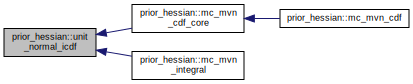
\includegraphics[width=350pt]{namespaceprior__hessian_ab76971b5aff40010d5c63fba454349b9_icgraph}
\end{center}
\end{figure}



\hypertarget{namespaceprior__hessian_1_1constants}{}\subsection{prior\+\_\+hessian\+:\+:constants Namespace Reference}
\label{namespaceprior__hessian_1_1constants}\index{prior\+\_\+hessian\+::constants@{prior\+\_\+hessian\+::constants}}
\subsubsection*{Variables}
\begin{DoxyCompactItemize}
\item 
const double \hyperlink{namespaceprior__hessian_1_1constants_aa1b2e54868f0913edd62e8029b829c43}{sqrt2} = std\+::sqrt(2.)
\item 
const double \hyperlink{namespaceprior__hessian_1_1constants_a083a6193aeb4fb1a3b244a132d25e1e3}{sqrt2\+\_\+inv} = 1./std\+::sqrt(2.)
\item 
const double \hyperlink{namespaceprior__hessian_1_1constants_a575039e0e575a200b1ba202c452ecbad}{sqrt2pi} = std\+::sqrt(2.$\ast$arma\+::datum\+::pi)
\item 
const double \hyperlink{namespaceprior__hessian_1_1constants_a7a6ae61175a9b764667984ec36da24bd}{sqrt2pi\+\_\+inv} = 1./std\+::sqrt(2.$\ast$arma\+::datum\+::pi)
\item 
const double \hyperlink{namespaceprior__hessian_1_1constants_a5a87faeb38eaf97a75f4d112cdaa4a8d}{log2pi} = std\+::log(2.$\ast$arma\+::datum\+::pi)
\end{DoxyCompactItemize}


\subsubsection{Variable Documentation}
\index{prior\+\_\+hessian\+::constants@{prior\+\_\+hessian\+::constants}!log2pi@{log2pi}}
\index{log2pi@{log2pi}!prior\+\_\+hessian\+::constants@{prior\+\_\+hessian\+::constants}}
\paragraph[{\texorpdfstring{log2pi}{log2pi}}]{\setlength{\rightskip}{0pt plus 5cm}const double prior\+\_\+hessian\+::constants\+::log2pi = std\+::log(2.$\ast$arma\+::datum\+::pi)}\hypertarget{namespaceprior__hessian_1_1constants_a5a87faeb38eaf97a75f4d112cdaa4a8d}{}\label{namespaceprior__hessian_1_1constants_a5a87faeb38eaf97a75f4d112cdaa4a8d}


Definition at line 19 of file util.\+cpp.



Referenced by prior\+\_\+hessian\+::\+Normal\+Dist\+::llh(), and prior\+\_\+hessian\+::\+Multivariate\+Normal\+Dist$<$ Ndim $>$\+::sample().

\index{prior\+\_\+hessian\+::constants@{prior\+\_\+hessian\+::constants}!sqrt2@{sqrt2}}
\index{sqrt2@{sqrt2}!prior\+\_\+hessian\+::constants@{prior\+\_\+hessian\+::constants}}
\paragraph[{\texorpdfstring{sqrt2}{sqrt2}}]{\setlength{\rightskip}{0pt plus 5cm}const double prior\+\_\+hessian\+::constants\+::sqrt2 = std\+::sqrt(2.)}\hypertarget{namespaceprior__hessian_1_1constants_aa1b2e54868f0913edd62e8029b829c43}{}\label{namespaceprior__hessian_1_1constants_aa1b2e54868f0913edd62e8029b829c43}


Definition at line 15 of file util.\+cpp.



Referenced by prior\+\_\+hessian\+::\+Normal\+Dist\+::icdf(), and prior\+\_\+hessian\+::unit\+\_\+normal\+\_\+icdf().

\index{prior\+\_\+hessian\+::constants@{prior\+\_\+hessian\+::constants}!sqrt2\+\_\+inv@{sqrt2\+\_\+inv}}
\index{sqrt2\+\_\+inv@{sqrt2\+\_\+inv}!prior\+\_\+hessian\+::constants@{prior\+\_\+hessian\+::constants}}
\paragraph[{\texorpdfstring{sqrt2\+\_\+inv}{sqrt2_inv}}]{\setlength{\rightskip}{0pt plus 5cm}const double prior\+\_\+hessian\+::constants\+::sqrt2\+\_\+inv = 1./std\+::sqrt(2.)}\hypertarget{namespaceprior__hessian_1_1constants_a083a6193aeb4fb1a3b244a132d25e1e3}{}\label{namespaceprior__hessian_1_1constants_a083a6193aeb4fb1a3b244a132d25e1e3}


Definition at line 16 of file util.\+cpp.



Referenced by prior\+\_\+hessian\+::\+Normal\+Dist\+::cdf().

\index{prior\+\_\+hessian\+::constants@{prior\+\_\+hessian\+::constants}!sqrt2pi@{sqrt2pi}}
\index{sqrt2pi@{sqrt2pi}!prior\+\_\+hessian\+::constants@{prior\+\_\+hessian\+::constants}}
\paragraph[{\texorpdfstring{sqrt2pi}{sqrt2pi}}]{\setlength{\rightskip}{0pt plus 5cm}const double prior\+\_\+hessian\+::constants\+::sqrt2pi = std\+::sqrt(2.$\ast$arma\+::datum\+::pi)}\hypertarget{namespaceprior__hessian_1_1constants_a575039e0e575a200b1ba202c452ecbad}{}\label{namespaceprior__hessian_1_1constants_a575039e0e575a200b1ba202c452ecbad}


Definition at line 17 of file util.\+cpp.

\index{prior\+\_\+hessian\+::constants@{prior\+\_\+hessian\+::constants}!sqrt2pi\+\_\+inv@{sqrt2pi\+\_\+inv}}
\index{sqrt2pi\+\_\+inv@{sqrt2pi\+\_\+inv}!prior\+\_\+hessian\+::constants@{prior\+\_\+hessian\+::constants}}
\paragraph[{\texorpdfstring{sqrt2pi\+\_\+inv}{sqrt2pi_inv}}]{\setlength{\rightskip}{0pt plus 5cm}const double prior\+\_\+hessian\+::constants\+::sqrt2pi\+\_\+inv = 1./std\+::sqrt(2.$\ast$arma\+::datum\+::pi)}\hypertarget{namespaceprior__hessian_1_1constants_a7a6ae61175a9b764667984ec36da24bd}{}\label{namespaceprior__hessian_1_1constants_a7a6ae61175a9b764667984ec36da24bd}


Definition at line 18 of file util.\+cpp.



Referenced by prior\+\_\+hessian\+::\+Normal\+Dist\+::pdf().


\hypertarget{namespaceprior__hessian_1_1CopulaDistImpl}{}\subsection{prior\+\_\+hessian\+:\+:Copula\+Dist\+Impl Namespace Reference}
\label{namespaceprior__hessian_1_1CopulaDistImpl}\index{prior\+\_\+hessian\+::\+Copula\+Dist\+Impl@{prior\+\_\+hessian\+::\+Copula\+Dist\+Impl}}
\subsubsection*{Classes}
\begin{DoxyCompactItemize}
\item 
class \hyperlink{classprior__hessian_1_1CopulaDistImpl_1_1CopulaDist}{Copula\+Dist}
\end{DoxyCompactItemize}

\hypertarget{namespaceprior__hessian_1_1detail}{}\subsection{prior\+\_\+hessian\+:\+:detail Namespace Reference}
\label{namespaceprior__hessian_1_1detail}\index{prior\+\_\+hessian\+::detail@{prior\+\_\+hessian\+::detail}}
\subsubsection*{Classes}
\begin{DoxyCompactItemize}
\item 
class \hyperlink{classprior__hessian_1_1detail_1_1dist__adaptor__traits}{dist\+\_\+adaptor\+\_\+traits}
\item 
struct \hyperlink{structprior__hessian_1_1detail_1_1dist__adaptor__traits_3_01CopulaDistImpl_1_1CopulaDist_3_01Cop7279db6753e87d864b5bda4f78bd9862}{dist\+\_\+adaptor\+\_\+traits$<$ Copula\+Dist\+Impl\+::\+Copula\+Dist$<$ Copula\+Template, Dist\+Ts... $>$ $>$}
\item 
struct \hyperlink{structprior__hessian_1_1detail_1_1dist__adaptor__traits_3_01GammaDist_01_4}{dist\+\_\+adaptor\+\_\+traits$<$ Gamma\+Dist $>$}
\item 
struct \hyperlink{structprior__hessian_1_1detail_1_1dist__adaptor__traits_3_01MultivariateNormalDist_3_01Ndim_01_4_01_4}{dist\+\_\+adaptor\+\_\+traits$<$ Multivariate\+Normal\+Dist$<$ Ndim $>$ $>$}
\item 
struct \hyperlink{structprior__hessian_1_1detail_1_1dist__adaptor__traits_3_01NormalDist_01_4}{dist\+\_\+adaptor\+\_\+traits$<$ Normal\+Dist $>$}
\item 
struct \hyperlink{structprior__hessian_1_1detail_1_1dist__adaptor__traits_3_01ParetoDist_01_4}{dist\+\_\+adaptor\+\_\+traits$<$ Pareto\+Dist $>$}
\item 
struct \hyperlink{structprior__hessian_1_1detail_1_1dist__adaptor__traits_3_01ScaledSymmetricBetaDist_01_4}{dist\+\_\+adaptor\+\_\+traits$<$ Scaled\+Symmetric\+Beta\+Dist $>$}
\item 
struct \hyperlink{structprior__hessian_1_1detail_1_1dist__adaptor__traits_3_01SymmetricBetaDist_01_4}{dist\+\_\+adaptor\+\_\+traits$<$ Symmetric\+Beta\+Dist $>$}
\item 
struct \hyperlink{structprior__hessian_1_1detail_1_1dist__adaptor__traits_3_01TruncatedGammaDist_01_4}{dist\+\_\+adaptor\+\_\+traits$<$ Truncated\+Gamma\+Dist $>$}
\item 
struct \hyperlink{structprior__hessian_1_1detail_1_1dist__adaptor__traits_3_01TruncatedMultivariateNormalDist_3_01Ndim_01_4_01_4}{dist\+\_\+adaptor\+\_\+traits$<$ Truncated\+Multivariate\+Normal\+Dist$<$ Ndim $>$ $>$}
\item 
struct \hyperlink{structprior__hessian_1_1detail_1_1dist__adaptor__traits_3_01TruncatedNormalDist_01_4}{dist\+\_\+adaptor\+\_\+traits$<$ Truncated\+Normal\+Dist $>$}
\item 
struct \hyperlink{structprior__hessian_1_1detail_1_1dist__adaptor__traits_3_01TruncatedParetoDist_01_4}{dist\+\_\+adaptor\+\_\+traits$<$ Truncated\+Pareto\+Dist $>$}
\end{DoxyCompactItemize}
\subsubsection*{Typedefs}
\begin{DoxyCompactItemize}
\item 
{\footnotesize template$<$class DistT $>$ }\\using \hyperlink{namespaceprior__hessian_1_1detail_a00684f44608e5a5bf76458d81159f924}{Dist\+TraitsT} = \hyperlink{classprior__hessian_1_1detail_1_1dist__adaptor__traits}{detail\+::dist\+\_\+adaptor\+\_\+traits}$<$ std\+::decay\+\_\+t$<$ DistT $>$$>$
\end{DoxyCompactItemize}
\subsubsection*{Functions}
\begin{DoxyCompactItemize}
\item 
{\footnotesize template$<$class... Ts, std\+::size\+\_\+t... I$>$ }\\std\+::tuple$<$ \hyperlink{namespaceprior__hessian_a919f0d7f51ea845224ca7f03983508a9}{Bounds\+Adapted\+DistT}$<$ Ts $>$... $>$ \hyperlink{namespaceprior__hessian_1_1detail_a13ee7e8b01109559d15a98dcdc1949d3}{make\+\_\+adapted\+\_\+bounded\+\_\+dist\+\_\+tuple} (std\+::tuple$<$ Ts... $>$ \&\&dists, std\+::index\+\_\+sequence$<$ I... $>$)
\item 
{\footnotesize template$<$class... Ts, std\+::size\+\_\+t... I$>$ }\\std\+::tuple$<$ \hyperlink{namespaceprior__hessian_a919f0d7f51ea845224ca7f03983508a9}{Bounds\+Adapted\+DistT}$<$ Ts $>$... $>$ \hyperlink{namespaceprior__hessian_1_1detail_a112a6e8be541a29b2c8b366f26e6d72e}{make\+\_\+adapted\+\_\+bounded\+\_\+dist\+\_\+tuple} (const std\+::tuple$<$ Ts... $>$ \&dists, std\+::index\+\_\+sequence$<$ I... $>$)
\item 
{\footnotesize template$<$long N, long... I$>$ }\\\hyperlink{namespaceprior__hessian_a0b42fc70dec525d83fb2ac155d9ab974}{VecT} \hyperlink{namespaceprior__hessian_1_1detail_a94c4015a4b09f513fc7de59a15c9247c}{eulerian\+\_\+polynomial} ()
\end{DoxyCompactItemize}


\subsubsection{Typedef Documentation}
\index{prior\+\_\+hessian\+::detail@{prior\+\_\+hessian\+::detail}!Dist\+TraitsT@{Dist\+TraitsT}}
\index{Dist\+TraitsT@{Dist\+TraitsT}!prior\+\_\+hessian\+::detail@{prior\+\_\+hessian\+::detail}}
\paragraph[{\texorpdfstring{Dist\+TraitsT}{DistTraitsT}}]{\setlength{\rightskip}{0pt plus 5cm}template$<$class DistT $>$ using {\bf prior\+\_\+hessian\+::detail\+::\+Dist\+TraitsT} = typedef {\bf detail\+::dist\+\_\+adaptor\+\_\+traits}$<$std\+::decay\+\_\+t$<$DistT$>$$>$}\hypertarget{namespaceprior__hessian_1_1detail_a00684f44608e5a5bf76458d81159f924}{}\label{namespaceprior__hessian_1_1detail_a00684f44608e5a5bf76458d81159f924}
Type traits class for distribution type DistT.

The traits class describes the Adaptor classes applicable to each individual distribution 

Definition at line 52 of file Bounds\+Adapted\+Dist.\+h.



\subsubsection{Function Documentation}
\index{prior\+\_\+hessian\+::detail@{prior\+\_\+hessian\+::detail}!eulerian\+\_\+polynomial@{eulerian\+\_\+polynomial}}
\index{eulerian\+\_\+polynomial@{eulerian\+\_\+polynomial}!prior\+\_\+hessian\+::detail@{prior\+\_\+hessian\+::detail}}
\paragraph[{\texorpdfstring{eulerian\+\_\+polynomial()}{eulerian_polynomial()}}]{\setlength{\rightskip}{0pt plus 5cm}template$<$long N, long... I$>$ {\bf VecT} prior\+\_\+hessian\+::detail\+::eulerian\+\_\+polynomial (
\begin{DoxyParamCaption}
{}
\end{DoxyParamCaption}
)}\hypertarget{namespaceprior__hessian_1_1detail_a94c4015a4b09f513fc7de59a15c9247c}{}\label{namespaceprior__hessian_1_1detail_a94c4015a4b09f513fc7de59a15c9247c}


Definition at line 26 of file Eulerian\+Polynomial.\+h.

\index{prior\+\_\+hessian\+::detail@{prior\+\_\+hessian\+::detail}!make\+\_\+adapted\+\_\+bounded\+\_\+dist\+\_\+tuple@{make\+\_\+adapted\+\_\+bounded\+\_\+dist\+\_\+tuple}}
\index{make\+\_\+adapted\+\_\+bounded\+\_\+dist\+\_\+tuple@{make\+\_\+adapted\+\_\+bounded\+\_\+dist\+\_\+tuple}!prior\+\_\+hessian\+::detail@{prior\+\_\+hessian\+::detail}}
\paragraph[{\texorpdfstring{make\+\_\+adapted\+\_\+bounded\+\_\+dist\+\_\+tuple(std\+::tuple$<$ Ts... $>$ \&\&dists, std\+::index\+\_\+sequence$<$ I... $>$)}{make_adapted_bounded_dist_tuple(std::tuple< Ts... > &&dists, std::index_sequence< I... >)}}]{\setlength{\rightskip}{0pt plus 5cm}template$<$class... Ts, std\+::size\+\_\+t... I$>$ std\+::tuple$<${\bf Bounds\+Adapted\+DistT}$<$Ts$>$...$>$ prior\+\_\+hessian\+::detail\+::make\+\_\+adapted\+\_\+bounded\+\_\+dist\+\_\+tuple (
\begin{DoxyParamCaption}
\item[{std\+::tuple$<$ Ts... $>$ \&\&}]{dists, }
\item[{std\+::index\+\_\+sequence$<$ I... $>$}]{}
\end{DoxyParamCaption}
)}\hypertarget{namespaceprior__hessian_1_1detail_a13ee7e8b01109559d15a98dcdc1949d3}{}\label{namespaceprior__hessian_1_1detail_a13ee7e8b01109559d15a98dcdc1949d3}


Definition at line 66 of file Bounds\+Adapted\+Dist.\+h.



References prior\+\_\+hessian\+::make\+\_\+adapted\+\_\+bounded\+\_\+dist().



Referenced by prior\+\_\+hessian\+::make\+\_\+adapted\+\_\+bounded\+\_\+dist\+\_\+tuple().



Here is the call graph for this function\+:\nopagebreak
\begin{figure}[H]
\begin{center}
\leavevmode
\includegraphics[width=350pt]{namespaceprior__hessian_1_1detail_a13ee7e8b01109559d15a98dcdc1949d3_cgraph}
\end{center}
\end{figure}




Here is the caller graph for this function\+:\nopagebreak
\begin{figure}[H]
\begin{center}
\leavevmode
\includegraphics[width=350pt]{namespaceprior__hessian_1_1detail_a13ee7e8b01109559d15a98dcdc1949d3_icgraph}
\end{center}
\end{figure}


\index{prior\+\_\+hessian\+::detail@{prior\+\_\+hessian\+::detail}!make\+\_\+adapted\+\_\+bounded\+\_\+dist\+\_\+tuple@{make\+\_\+adapted\+\_\+bounded\+\_\+dist\+\_\+tuple}}
\index{make\+\_\+adapted\+\_\+bounded\+\_\+dist\+\_\+tuple@{make\+\_\+adapted\+\_\+bounded\+\_\+dist\+\_\+tuple}!prior\+\_\+hessian\+::detail@{prior\+\_\+hessian\+::detail}}
\paragraph[{\texorpdfstring{make\+\_\+adapted\+\_\+bounded\+\_\+dist\+\_\+tuple(const std\+::tuple$<$ Ts... $>$ \&dists, std\+::index\+\_\+sequence$<$ I... $>$)}{make_adapted_bounded_dist_tuple(const std::tuple< Ts... > &dists, std::index_sequence< I... >)}}]{\setlength{\rightskip}{0pt plus 5cm}template$<$class... Ts, std\+::size\+\_\+t... I$>$ std\+::tuple$<${\bf Bounds\+Adapted\+DistT}$<$Ts$>$...$>$ prior\+\_\+hessian\+::detail\+::make\+\_\+adapted\+\_\+bounded\+\_\+dist\+\_\+tuple (
\begin{DoxyParamCaption}
\item[{const std\+::tuple$<$ Ts... $>$ \&}]{dists, }
\item[{std\+::index\+\_\+sequence$<$ I... $>$}]{}
\end{DoxyParamCaption}
)}\hypertarget{namespaceprior__hessian_1_1detail_a112a6e8be541a29b2c8b366f26e6d72e}{}\label{namespaceprior__hessian_1_1detail_a112a6e8be541a29b2c8b366f26e6d72e}


Definition at line 73 of file Bounds\+Adapted\+Dist.\+h.



References prior\+\_\+hessian\+::make\+\_\+adapted\+\_\+bounded\+\_\+dist().



Here is the call graph for this function\+:\nopagebreak
\begin{figure}[H]
\begin{center}
\leavevmode
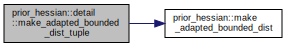
\includegraphics[width=350pt]{namespaceprior__hessian_1_1detail_a112a6e8be541a29b2c8b366f26e6d72e_cgraph}
\end{center}
\end{figure}



\hypertarget{namespaceprior__hessian_1_1genz}{}\subsection{prior\+\_\+hessian\+:\+:genz Namespace Reference}
\label{namespaceprior__hessian_1_1genz}\index{prior\+\_\+hessian\+::genz@{prior\+\_\+hessian\+::genz}}
\subsubsection*{Namespaces}
\begin{DoxyCompactItemize}
\item 
 \hyperlink{namespaceprior__hessian_1_1genz_1_1fortran}{fortran}
\end{DoxyCompactItemize}
\subsubsection*{Functions}
\begin{DoxyCompactItemize}
\item 
{\footnotesize template$<$class Vec , class Mat $>$ }\\double \hyperlink{namespaceprior__hessian_1_1genz_a5462d1271384fa7431ee84709c0f8a88}{mvn\+\_\+cdf\+\_\+genz} (const Vec \&b, const Mat \&S, double \&error)
\end{DoxyCompactItemize}


\subsubsection{Function Documentation}
\index{prior\+\_\+hessian\+::genz@{prior\+\_\+hessian\+::genz}!mvn\+\_\+cdf\+\_\+genz@{mvn\+\_\+cdf\+\_\+genz}}
\index{mvn\+\_\+cdf\+\_\+genz@{mvn\+\_\+cdf\+\_\+genz}!prior\+\_\+hessian\+::genz@{prior\+\_\+hessian\+::genz}}
\paragraph[{\texorpdfstring{mvn\+\_\+cdf\+\_\+genz(const Vec \&b, const Mat \&\+S, double \&error)}{mvn_cdf_genz(const Vec &b, const Mat &S, double &error)}}]{\setlength{\rightskip}{0pt plus 5cm}template$<$class Vec , class Mat $>$ double prior\+\_\+hessian\+::genz\+::mvn\+\_\+cdf\+\_\+genz (
\begin{DoxyParamCaption}
\item[{const Vec \&}]{b, }
\item[{const Mat \&}]{S, }
\item[{double \&}]{error}
\end{DoxyParamCaption}
)}\hypertarget{namespaceprior__hessian_1_1genz_a5462d1271384fa7431ee84709c0f8a88}{}\label{namespaceprior__hessian_1_1genz_a5462d1271384fa7431ee84709c0f8a88}


Definition at line 217 of file mvn\+\_\+cdf.\+h.



References prior\+\_\+hessian\+::genz\+::fortran\+::mvndst\+\_\+().



Referenced by prior\+\_\+hessian\+::\+Multivariate\+Normal\+Dist$<$ Ndim $>$\+::cdf().



Here is the call graph for this function\+:\nopagebreak
\begin{figure}[H]
\begin{center}
\leavevmode
\includegraphics[width=312pt]{namespaceprior__hessian_1_1genz_a5462d1271384fa7431ee84709c0f8a88_cgraph}
\end{center}
\end{figure}




Here is the caller graph for this function\+:\nopagebreak
\begin{figure}[H]
\begin{center}
\leavevmode
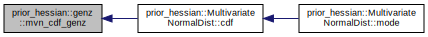
\includegraphics[width=350pt]{namespaceprior__hessian_1_1genz_a5462d1271384fa7431ee84709c0f8a88_icgraph}
\end{center}
\end{figure}



\hypertarget{namespaceprior__hessian_1_1genz_1_1fortran}{}\subsection{prior\+\_\+hessian\+:\+:genz\+:\+:fortran Namespace Reference}
\label{namespaceprior__hessian_1_1genz_1_1fortran}\index{prior\+\_\+hessian\+::genz\+::fortran@{prior\+\_\+hessian\+::genz\+::fortran}}
\subsubsection*{Functions}
\begin{DoxyCompactItemize}
\item 
int \hyperlink{namespaceprior__hessian_1_1genz_1_1fortran_a3aa3e81ace64048700679aa6ab8f0879}{mvndst\+\_\+} (int $\ast$n, double lower\mbox{[}$\,$\mbox{]}, double upper\mbox{[}$\,$\mbox{]}, int infin\mbox{[}$\,$\mbox{]}, double correl\mbox{[}$\,$\mbox{]}, int $\ast$maxpts, double $\ast$abseps, double $\ast$releps, double $\ast$error, double $\ast$value, int $\ast$inform)
\end{DoxyCompactItemize}


\subsubsection{Function Documentation}
\index{prior\+\_\+hessian\+::genz\+::fortran@{prior\+\_\+hessian\+::genz\+::fortran}!mvndst\+\_\+@{mvndst\+\_\+}}
\index{mvndst\+\_\+@{mvndst\+\_\+}!prior\+\_\+hessian\+::genz\+::fortran@{prior\+\_\+hessian\+::genz\+::fortran}}
\paragraph[{\texorpdfstring{mvndst\+\_\+(int $\ast$n, double lower[], double upper[], int infin[], double correl[], int $\ast$maxpts, double $\ast$abseps, double $\ast$releps, double $\ast$error, double $\ast$value, int $\ast$inform)}{mvndst_(int *n, double lower[], double upper[], int infin[], double correl[], int *maxpts, double *abseps, double *releps, double *error, double *value, int *inform)}}]{\setlength{\rightskip}{0pt plus 5cm}int prior\+\_\+hessian\+::genz\+::fortran\+::mvndst\+\_\+ (
\begin{DoxyParamCaption}
\item[{int $\ast$}]{n, }
\item[{double}]{lower\mbox{[}$\,$\mbox{]}, }
\item[{double}]{upper\mbox{[}$\,$\mbox{]}, }
\item[{int}]{infin\mbox{[}$\,$\mbox{]}, }
\item[{double}]{correl\mbox{[}$\,$\mbox{]}, }
\item[{int $\ast$}]{maxpts, }
\item[{double $\ast$}]{abseps, }
\item[{double $\ast$}]{releps, }
\item[{double $\ast$}]{error, }
\item[{double $\ast$}]{value, }
\item[{int $\ast$}]{inform}
\end{DoxyParamCaption}
)}\hypertarget{namespaceprior__hessian_1_1genz_1_1fortran_a3aa3e81ace64048700679aa6ab8f0879}{}\label{namespaceprior__hessian_1_1genz_1_1fortran_a3aa3e81ace64048700679aa6ab8f0879}


Referenced by prior\+\_\+hessian\+::genz\+::mvn\+\_\+cdf\+\_\+genz().



Here is the caller graph for this function\+:\nopagebreak
\begin{figure}[H]
\begin{center}
\leavevmode
\includegraphics[width=350pt]{namespaceprior__hessian_1_1genz_1_1fortran_a3aa3e81ace64048700679aa6ab8f0879_icgraph}
\end{center}
\end{figure}



\hypertarget{namespaceprior__hessian_1_1helpers}{}\subsection{prior\+\_\+hessian\+:\+:helpers Namespace Reference}
\label{namespaceprior__hessian_1_1helpers}\index{prior\+\_\+hessian\+::helpers@{prior\+\_\+hessian\+::helpers}}
\subsubsection*{Functions}
\begin{DoxyCompactItemize}
\item 
{\footnotesize template$<$class Vec , class Mat $>$ }\\double \hyperlink{namespaceprior__hessian_1_1helpers_a5d1bbe705c849e9c225a831c853be8a7}{compute\+\_\+quadratic\+\_\+from\+\_\+symmetric} (\hyperlink{namespaceprior__hessian_aa8d589f74e88bfa3b5750118acd1ab78}{IdxT} Ndim, const Vec \&v, const Mat \&A)
\end{DoxyCompactItemize}


\subsubsection{Function Documentation}
\index{prior\+\_\+hessian\+::helpers@{prior\+\_\+hessian\+::helpers}!compute\+\_\+quadratic\+\_\+from\+\_\+symmetric@{compute\+\_\+quadratic\+\_\+from\+\_\+symmetric}}
\index{compute\+\_\+quadratic\+\_\+from\+\_\+symmetric@{compute\+\_\+quadratic\+\_\+from\+\_\+symmetric}!prior\+\_\+hessian\+::helpers@{prior\+\_\+hessian\+::helpers}}
\paragraph[{\texorpdfstring{compute\+\_\+quadratic\+\_\+from\+\_\+symmetric(\+Idx\+T Ndim, const Vec \&v, const Mat \&\+A)}{compute_quadratic_from_symmetric(IdxT Ndim, const Vec &v, const Mat &A)}}]{\setlength{\rightskip}{0pt plus 5cm}template$<$class Vec , class Mat $>$ double prior\+\_\+hessian\+::helpers\+::compute\+\_\+quadratic\+\_\+from\+\_\+symmetric (
\begin{DoxyParamCaption}
\item[{{\bf IdxT}}]{Ndim, }
\item[{const Vec \&}]{v, }
\item[{const Mat \&}]{A}
\end{DoxyParamCaption}
)}\hypertarget{namespaceprior__hessian_1_1helpers_a5d1bbe705c849e9c225a831c853be8a7}{}\label{namespaceprior__hessian_1_1helpers_a5d1bbe705c849e9c225a831c853be8a7}


Definition at line 137 of file Multivariate\+Normal\+Dist.\+h.



References prior\+\_\+hessian\+::square().



Referenced by prior\+\_\+hessian\+::\+Multivariate\+Normal\+Dist$<$ Ndim $>$\+::rllh().



Here is the call graph for this function\+:\nopagebreak
\begin{figure}[H]
\begin{center}
\leavevmode
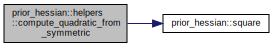
\includegraphics[width=345pt]{namespaceprior__hessian_1_1helpers_a5d1bbe705c849e9c225a831c853be8a7_cgraph}
\end{center}
\end{figure}




Here is the caller graph for this function\+:\nopagebreak
\begin{figure}[H]
\begin{center}
\leavevmode
\includegraphics[width=350pt]{namespaceprior__hessian_1_1helpers_a5d1bbe705c849e9c225a831c853be8a7_icgraph}
\end{center}
\end{figure}



\hypertarget{namespaceprior__hessian_1_1mcmc}{}\subsection{prior\+\_\+hessian\+:\+:mcmc Namespace Reference}
\label{namespaceprior__hessian_1_1mcmc}\index{prior\+\_\+hessian\+::mcmc@{prior\+\_\+hessian\+::mcmc}}
\subsubsection*{Classes}
\begin{DoxyCompactItemize}
\item 
class \hyperlink{classprior__hessian_1_1mcmc_1_1MCMCData}{M\+C\+M\+C\+Data}
\end{DoxyCompactItemize}

\hypertarget{namespaceprior__hessian_1_1meta}{}\subsection{prior\+\_\+hessian\+:\+:meta Namespace Reference}
\label{namespaceprior__hessian_1_1meta}\index{prior\+\_\+hessian\+::meta@{prior\+\_\+hessian\+::meta}}


Class templates to utilize sequencing behavior of std\+::initializer\+\_\+list expressions.  


\subsubsection*{Classes}
\begin{DoxyCompactItemize}
\item 
struct \hyperlink{structprior__hessian_1_1meta_1_1all__dists__are__bounded}{all\+\_\+dists\+\_\+are\+\_\+bounded}
\item 
struct \hyperlink{structprior__hessian_1_1meta_1_1conjunction}{conjunction}
\item 
struct \hyperlink{structprior__hessian_1_1meta_1_1conjunction_3_01B1_01_4}{conjunction$<$ B1 $>$}
\item 
struct \hyperlink{structprior__hessian_1_1meta_1_1conjunction_3_01B1_00_01Bn_8_8_8_01_4}{conjunction$<$ B1, Bn... $>$}
\item 
struct \hyperlink{structprior__hessian_1_1meta_1_1disjunction}{disjunction}
\item 
struct \hyperlink{structprior__hessian_1_1meta_1_1disjunction_3_01B1_01_4}{disjunction$<$ B1 $>$}
\item 
struct \hyperlink{structprior__hessian_1_1meta_1_1disjunction_3_01B1_00_01Bn_8_8_8_01_4}{disjunction$<$ B1, Bn... $>$}
\item 
class \hyperlink{classprior__hessian_1_1meta_1_1is__copula}{is\+\_\+copula}
\item 
struct \hyperlink{structprior__hessian_1_1meta_1_1is__numeric__template__of}{is\+\_\+numeric\+\_\+template\+\_\+of}
\item 
struct \hyperlink{structprior__hessian_1_1meta_1_1is__numeric__template__of_3_01ClassNumericTemplate_00_01ClassNum9ff24e61e3d3187d075a4a72dee66cb3}{is\+\_\+numeric\+\_\+template\+\_\+of$<$ Class\+Numeric\+Template, Class\+Numeric\+Template$<$ Is... $>$ $>$}
\item 
class \hyperlink{classprior__hessian_1_1meta_1_1is__subclass__of__numeric__template}{is\+\_\+subclass\+\_\+of\+\_\+numeric\+\_\+template}
\item 
struct \hyperlink{structprior__hessian_1_1meta_1_1is__template__of}{is\+\_\+template\+\_\+of}
\item 
struct \hyperlink{structprior__hessian_1_1meta_1_1is__template__of_3_01ClassTemplate_00_01ClassTemplate_3_01Ts_8_8_8_01_4_01_4}{is\+\_\+template\+\_\+of$<$ Class\+Template, Class\+Template$<$ Ts... $>$ $>$}
\end{DoxyCompactItemize}
\subsubsection*{Typedefs}
\begin{DoxyCompactItemize}
\item 
{\footnotesize template$<$class... Dist\+Ts$>$ }\\using \hyperlink{namespaceprior__hessian_1_1meta_a1f28a9142fc5442b2ba3cf722169578a}{Constructable\+If\+All\+Dists\+Are\+BoundedT} = std\+::enable\+\_\+if$<$ \hyperlink{structprior__hessian_1_1meta_1_1all__dists__are__bounded}{all\+\_\+dists\+\_\+are\+\_\+bounded}$<$ Dist\+Ts... $>$\+::value, bool $>$
\item 
{\footnotesize template$<$class... Dist\+Ts$>$ }\\using \hyperlink{namespaceprior__hessian_1_1meta_a33414fea85f38ec07f5b6a750be5656b}{Constructable\+If\+Not\+All\+Dists\+Are\+BoundedT} = std\+::enable\+\_\+if$<$!\hyperlink{structprior__hessian_1_1meta_1_1all__dists__are__bounded}{all\+\_\+dists\+\_\+are\+\_\+bounded}$<$ Dist\+Ts... $>$\+::value, bool $>$
\item 
{\footnotesize template$<$template$<$ template$<$ int $>$ class, class... $>$ class CopulaT, class U $>$ }\\using \hyperlink{namespaceprior__hessian_1_1meta_a18d532e255e9785cca33c9bf8b932adf}{Constructable\+If\+Is\+CopulaT} = std\+::enable\+\_\+if\+\_\+t$<$ \hyperlink{classprior__hessian_1_1meta_1_1is__copula}{is\+\_\+copula}$<$ CopulaT, U $>$\+::value,bool $>$
\item 
{\footnotesize template$<$class ReturnT , class BoolT $>$ }\\using \hyperlink{namespaceprior__hessian_1_1meta_a3fb9317007d5f1b3825cbfd69d491374}{Return\+IfT} = std\+::enable\+\_\+if\+\_\+t$<$ Bool\+T\+::value, ReturnT $>$
\item 
{\footnotesize template$<$bool val$>$ }\\using \hyperlink{namespaceprior__hessian_1_1meta_aa8f9847c6c56ca1f8530657d74bb9a99}{Constructable\+If} = std\+::enable\+\_\+if\+\_\+t$<$ val, bool $>$
\item 
{\footnotesize template$<$bool val$>$ }\\using \hyperlink{namespaceprior__hessian_1_1meta_a23667341714ecaa72ef51dafae35ee60}{Constructable\+If\+Not} = std\+::enable\+\_\+if\+\_\+t$<$!val, bool $>$
\item 
{\footnotesize template$<$class T , class SelfT $>$ }\\using \hyperlink{namespaceprior__hessian_1_1meta_a1aa5afbb3de8629472e4cd3fbabf13ae}{Constructable\+If\+Not\+SelfT} = std\+::enable\+\_\+if\+\_\+t$<$!std\+::is\+\_\+same$<$ std\+::decay\+\_\+t$<$ T $>$, SelfT $>$\+::value, bool $>$
\item 
{\footnotesize template$<$class T , class BaseT $>$ }\\using \hyperlink{namespaceprior__hessian_1_1meta_abc650c6661b53cac162bce78cc6c4830}{Enable\+If\+SubclassT} = std\+::enable\+\_\+if\+\_\+t$<$ std\+::is\+\_\+base\+\_\+of$<$ std\+::remove\+\_\+reference\+\_\+t$<$ BaseT $>$, std\+::remove\+\_\+reference\+\_\+t$<$ T $>$$>$\+::value $>$
\item 
{\footnotesize template$<$class T , template$<$ int $>$ class Class\+Numeric\+Template$>$ }\\using \hyperlink{namespaceprior__hessian_1_1meta_a722a7d9905845f2dd08a95b2ddecc10e}{Enable\+If\+Subclass\+Of\+Numeric\+TemplateT} = std\+::enable\+\_\+if\+\_\+t$<$ \hyperlink{classprior__hessian_1_1meta_1_1is__subclass__of__numeric__template}{is\+\_\+subclass\+\_\+of\+\_\+numeric\+\_\+template}$<$ Class\+Numeric\+Template, std\+::remove\+\_\+reference\+\_\+t$<$ T $>$$>$\+::value $>$
\item 
{\footnotesize template$<$class ReturnT , class T , template$<$ int $>$ class Class\+Numeric\+Template$>$ }\\using \hyperlink{namespaceprior__hessian_1_1meta_a05320676e0242ae8def463a1afee362c}{Return\+If\+Subclass\+Of\+Numeric\+TemplateT} = std\+::enable\+\_\+if\+\_\+t$<$ \hyperlink{classprior__hessian_1_1meta_1_1is__subclass__of__numeric__template}{is\+\_\+subclass\+\_\+of\+\_\+numeric\+\_\+template}$<$ Class\+Numeric\+Template, std\+::remove\+\_\+reference\+\_\+t$<$ T $>$$>$\+::value, ReturnT $>$
\item 
{\footnotesize template$<$class T , class SelfT $>$ }\\using \hyperlink{namespaceprior__hessian_1_1meta_ad84d45d1d36f0fbf216f1380d638d22a}{Enable\+If\+Not\+Is\+SelfT} = std\+::enable\+\_\+if\+\_\+t$<$ !std\+::is\+\_\+same$<$ std\+::decay\+\_\+t$<$ T $>$, SelfT $>$\+::value $>$
\item 
{\footnotesize template$<$class ReturnT , class T , class BaseT $>$ }\\using \hyperlink{namespaceprior__hessian_1_1meta_a955cdfa0e628ca7f179af6ab70e87cdd}{Return\+If\+SubclassT} = std\+::enable\+\_\+if\+\_\+t$<$ std\+::is\+\_\+base\+\_\+of$<$ std\+::remove\+\_\+reference\+\_\+t$<$ BaseT $>$, std\+::remove\+\_\+reference\+\_\+t$<$ T $>$$>$\+::value, ReturnT $>$
\item 
{\footnotesize template$<$class BaseT , class... Ts$>$ }\\using \hyperlink{namespaceprior__hessian_1_1meta_a0413ae4eb881eabac578a1283fbff570}{Enable\+If\+Is\+Superclass\+Of\+AllT} = std\+::enable\+\_\+if\+\_\+t$<$ \hyperlink{structprior__hessian_1_1meta_1_1conjunction}{conjunction}$<$ std\+::is\+\_\+base\+\_\+of$<$ std\+::remove\+\_\+reference\+\_\+t$<$ BaseT $>$, std\+::remove\+\_\+reference\+\_\+t$<$ Ts $>$$>$... $>$\+::value $>$
\item 
{\footnotesize template$<$class T , template$<$ typename... $>$ class Class\+Template$>$ }\\using \hyperlink{namespaceprior__hessian_1_1meta_aeab241d6ef85931a7a35a030036ad6b0}{Enable\+If\+Instantiated\+FromT} = std\+::enable\+\_\+if\+\_\+t$<$ \hyperlink{structprior__hessian_1_1meta_1_1is__template__of}{is\+\_\+template\+\_\+of}$<$ Class\+Template, std\+::remove\+\_\+reference\+\_\+t$<$ T $>$$>$\+::value $>$
\item 
{\footnotesize template$<$class T , template$<$ int $>$ class Class\+Template$>$ }\\using \hyperlink{namespaceprior__hessian_1_1meta_a4b18f40222c75d1a3f9955464799c452}{Enable\+If\+Instantiated\+From\+NumericT} = std\+::enable\+\_\+if\+\_\+t$<$ \hyperlink{structprior__hessian_1_1meta_1_1is__numeric__template__of}{is\+\_\+numeric\+\_\+template\+\_\+of}$<$ Class\+Template, std\+::remove\+\_\+reference\+\_\+t$<$ T $>$$>$\+::value $>$
\item 
{\footnotesize template$<$class ReturnT , class T , template$<$ int $>$ class Class\+Template$>$ }\\using \hyperlink{namespaceprior__hessian_1_1meta_a408d81bee769664002f490e4a08b9944}{Return\+If\+Instantiated\+From\+NumericT} = std\+::enable\+\_\+if\+\_\+t$<$ \hyperlink{structprior__hessian_1_1meta_1_1is__numeric__template__of}{is\+\_\+numeric\+\_\+template\+\_\+of}$<$ Class\+Template, std\+::remove\+\_\+reference\+\_\+t$<$ T $>$$>$\+::value, ReturnT $>$
\item 
{\footnotesize template$<$class T , template$<$ typename... $>$ class Class\+Template$>$ }\\using \hyperlink{namespaceprior__hessian_1_1meta_a4d2b4afd50ec9adfdf0ad0ba0f690360}{Enable\+If\+Not\+Instantiated\+FromT} = std\+::enable\+\_\+if\+\_\+t$<$ !\hyperlink{structprior__hessian_1_1meta_1_1is__template__of}{is\+\_\+template\+\_\+of}$<$ Class\+Template, std\+::remove\+\_\+reference\+\_\+t$<$ T $>$$>$\+::value $>$
\item 
{\footnotesize template$<$class ReturnT , class TestT , template$<$ typename... $>$ class Class\+Template$>$ }\\using \hyperlink{namespaceprior__hessian_1_1meta_ab7bb340f7fc79b7a874c3d407fca091d}{Return\+If\+Instantiated\+FromT} = std\+::enable\+\_\+if\+\_\+t$<$ \hyperlink{structprior__hessian_1_1meta_1_1is__template__of}{is\+\_\+template\+\_\+of}$<$ Class\+Template, std\+::remove\+\_\+reference\+\_\+t$<$ TestT $>$$>$\+::value, ReturnT $>$
\item 
{\footnotesize template$<$class ReturnT , class TestT , template$<$ typename... $>$ class Class\+Template$>$ }\\using \hyperlink{namespaceprior__hessian_1_1meta_aea50a7973fa87d00d93e526c23d14549}{Return\+If\+Not\+Instantiated\+FromT} = std\+::enable\+\_\+if\+\_\+t$<$ !\hyperlink{structprior__hessian_1_1meta_1_1is__template__of}{is\+\_\+template\+\_\+of}$<$ Class\+Template, std\+::remove\+\_\+reference\+\_\+t$<$ TestT $>$$>$\+::value, ReturnT $>$
\item 
{\footnotesize template$<$template$<$ typename $>$ class Class\+Template, class... Ts$>$ }\\using \hyperlink{namespaceprior__hessian_1_1meta_a6c1ba653f64db9c1887e74c50ab257b1}{Enable\+If\+Is\+Template\+For\+AllT} = std\+::enable\+\_\+if\+\_\+t$<$ \hyperlink{structprior__hessian_1_1meta_1_1conjunction}{conjunction}$<$ \hyperlink{structprior__hessian_1_1meta_1_1is__template__of}{is\+\_\+template\+\_\+of}$<$ Class\+Template, std\+::remove\+\_\+reference\+\_\+t$<$ Ts $>$$>$... $>$\+::value $>$
\item 
{\footnotesize template$<$template$<$ typename... $>$ class Class\+Template, class... Ts$>$ }\\using \hyperlink{namespaceprior__hessian_1_1meta_a48175b9bfd69aa8a555323c758403a62}{Constructable\+If\+Is\+Template\+For\+AllT} = std\+::enable\+\_\+if\+\_\+t$<$ \hyperlink{structprior__hessian_1_1meta_1_1conjunction}{conjunction}$<$ \hyperlink{structprior__hessian_1_1meta_1_1is__template__of}{is\+\_\+template\+\_\+of}$<$ Class\+Template, std\+::remove\+\_\+reference\+\_\+t$<$ Ts $>$$>$... $>$\+::value, bool $>$
\item 
{\footnotesize template$<$class Super\+Class , class T $>$ }\\using \hyperlink{namespaceprior__hessian_1_1meta_ac41c6affb6f4ae3fb6ea0abd23a3b10d}{Constructable\+If\+Is\+Super\+ClassT} = std\+::enable\+\_\+if\+\_\+t$<$ std\+::is\+\_\+base\+\_\+of$<$ std\+::remove\+\_\+reference\+\_\+t$<$ Super\+Class $>$, std\+::remove\+\_\+reference\+\_\+t$<$ T $>$$>$\+::value, bool $>$
\item 
{\footnotesize template$<$class Super\+Class , class... Ts$>$ }\\using \hyperlink{namespaceprior__hessian_1_1meta_a4e077ce0021239d133049cf40e8f163e}{Constructable\+If\+Is\+Super\+Class\+For\+AllT} = std\+::enable\+\_\+if\+\_\+t$<$ \hyperlink{structprior__hessian_1_1meta_1_1conjunction}{conjunction}$<$ std\+::is\+\_\+base\+\_\+of$<$ std\+::remove\+\_\+reference\+\_\+t$<$ Super\+Class $>$, std\+::remove\+\_\+reference\+\_\+t$<$ Ts $>$$>$... $>$\+::value, bool $>$
\item 
{\footnotesize template$<$class T , template$<$ int $>$ class Class\+Template$>$ }\\using \hyperlink{namespaceprior__hessian_1_1meta_af9f0f80d3bced7421046f8eed53d21f1}{Constructable\+If\+Instantiated\+From\+NumericT} = std\+::enable\+\_\+if\+\_\+t$<$ \hyperlink{structprior__hessian_1_1meta_1_1is__numeric__template__of}{is\+\_\+numeric\+\_\+template\+\_\+of}$<$ Class\+Template, std\+::remove\+\_\+reference\+\_\+t$<$ T $>$$>$\+::value, bool $>$
\item 
{\footnotesize template$<$class T $>$ }\\using \hyperlink{namespaceprior__hessian_1_1meta_a3ea8e11b3e91986909abe98764a02990}{Enable\+If\+Is\+Not\+TupleT} = std\+::enable\+\_\+if\+\_\+t$<$ !\hyperlink{structprior__hessian_1_1meta_1_1is__template__of}{is\+\_\+template\+\_\+of}$<$ std\+::tuple, std\+::remove\+\_\+reference\+\_\+t$<$ T $>$$>$\+::value $>$
\item 
{\footnotesize template$<$class... Ts$>$ }\\using \hyperlink{namespaceprior__hessian_1_1meta_a20687a1e7c6127dea649f7719ff455d3}{Enable\+If\+Non\+Empty} = std\+::enable\+\_\+if\+\_\+t$<$ (sizeof...(Ts)$>$0) $>$
\item 
{\footnotesize template$<$class... Ts$>$ }\\using \hyperlink{namespaceprior__hessian_1_1meta_a4c0f2ff12f5d30e05ef9ca55a3f35318}{Enable\+If\+All\+Are\+Not\+TupleT} = std\+::enable\+\_\+if\+\_\+t$<$ !\hyperlink{structprior__hessian_1_1meta_1_1disjunction}{disjunction}$<$ \hyperlink{structprior__hessian_1_1meta_1_1is__template__of}{is\+\_\+template\+\_\+of}$<$ std\+::tuple, std\+::remove\+\_\+reference\+\_\+t$<$ Ts $>$$>$... $>$\+::value $>$
\item 
{\footnotesize template$<$class SelfT , class T $>$ }\\using \hyperlink{namespaceprior__hessian_1_1meta_a334715ebe83bc8b5ece276b960071701}{Enable\+If\+Is\+Not\+Tuple\+And\+Is\+Not\+SelfT} = std\+::enable\+\_\+if\+\_\+t$<$ !\hyperlink{structprior__hessian_1_1meta_1_1is__template__of}{is\+\_\+template\+\_\+of}$<$ std\+::tuple, std\+::remove\+\_\+reference\+\_\+t$<$ T $>$$>$\+::value \&\&!std\+::is\+\_\+same$<$ std\+::decay\+\_\+t$<$ T $>$, SelfT $>$\+::value $>$
\item 
{\footnotesize template$<$class T , class... Ts$>$ }\\using \hyperlink{namespaceprior__hessian_1_1meta_a5eaabc649c9629ae8f49d45c3141c4b5}{Constructable\+If\+All\+Are\+Not\+Tuple\+And\+Are\+NotT} = std\+::enable\+\_\+if\+\_\+t$<$ !\hyperlink{structprior__hessian_1_1meta_1_1disjunction}{disjunction}$<$ \hyperlink{structprior__hessian_1_1meta_1_1is__template__of}{is\+\_\+template\+\_\+of}$<$ std\+::tuple, std\+::remove\+\_\+reference\+\_\+t$<$ Ts $>$$>$... $>$\+::value \&\&!\hyperlink{structprior__hessian_1_1meta_1_1disjunction}{disjunction}$<$ std\+::is\+\_\+same$<$ std\+::decay\+\_\+t$<$ Ts $>$, T $>$... $>$\+::value, bool $>$
\item 
{\footnotesize template$<$class Dist , class Base\+Dist $>$ }\\using \hyperlink{namespaceprior__hessian_1_1meta_a7dcd55f8c696cfac1fe7872289c4d3e1}{Derived\+From} = std\+::enable\+\_\+if\+\_\+t$<$ std\+::is\+\_\+base\+\_\+of$<$ std\+::decay\+\_\+t$<$ \hyperlink{classprior__hessian_1_1BaseDist}{Base\+Dist} $>$, std\+::decay\+\_\+t$<$ Dist $>$$>$\+::value, std\+::decay\+\_\+t$<$ Dist $>$$>$
\end{DoxyCompactItemize}
\subsubsection*{Functions}
\begin{DoxyCompactItemize}
\item 
{\footnotesize template$<$class T  = int$>$ }\\void \hyperlink{namespaceprior__hessian_1_1meta_a179314ad7ba735849c4095e735374ab2}{call\+\_\+in\+\_\+order} (std\+::initializer\+\_\+list$<$ T $>$)
\item 
{\footnotesize template$<$class Input\+Iterator , class ResultT , class Binary\+Operation $>$ }\\\hyperlink{Meta_8h_a4f9105f0c435f5a50cc6000252e92575}{P\+R\+I\+O\+R\+\_\+\+H\+E\+S\+S\+I\+A\+N\+\_\+\+M\+E\+T\+A\+\_\+\+C\+O\+N\+S\+T\+E\+X\+PR} ResultT \hyperlink{namespaceprior__hessian_1_1meta_a8dd1d78533f7011bebda7009c0591041}{constexpr\+\_\+accumulate} (Input\+Iterator first, Input\+Iterator last, ResultT init, Binary\+Operation op)
\item 
\hyperlink{Meta_8h_a4f9105f0c435f5a50cc6000252e92575}{P\+R\+I\+O\+R\+\_\+\+H\+E\+S\+S\+I\+A\+N\+\_\+\+M\+E\+T\+A\+\_\+\+C\+O\+N\+S\+T\+E\+X\+PR} bool \hyperlink{namespaceprior__hessian_1_1meta_add11951e7edc2c231ca52c32ac0ee07b}{logical\+\_\+and\+\_\+in\+\_\+order} (std\+::initializer\+\_\+list$<$ bool $>$ L)
\item 
{\footnotesize template$<$class T $>$ }\\\hyperlink{Meta_8h_a4f9105f0c435f5a50cc6000252e92575}{P\+R\+I\+O\+R\+\_\+\+H\+E\+S\+S\+I\+A\+N\+\_\+\+M\+E\+T\+A\+\_\+\+C\+O\+N\+S\+T\+E\+X\+PR} T \hyperlink{namespaceprior__hessian_1_1meta_ab09470f06d05f5c58e249a03ef19242f}{sum\+\_\+in\+\_\+order} (std\+::initializer\+\_\+list$<$ T $>$ L)
\item 
{\footnotesize template$<$class T $>$ }\\\hyperlink{Meta_8h_a4f9105f0c435f5a50cc6000252e92575}{P\+R\+I\+O\+R\+\_\+\+H\+E\+S\+S\+I\+A\+N\+\_\+\+M\+E\+T\+A\+\_\+\+C\+O\+N\+S\+T\+E\+X\+PR} T \hyperlink{namespaceprior__hessian_1_1meta_a32068030d513a09bf78340f87be83639}{prod\+\_\+in\+\_\+order} (std\+::initializer\+\_\+list$<$ T $>$ L)
\end{DoxyCompactItemize}


\subsubsection{Detailed Description}
Class templates to utilize sequencing behavior of std\+::initializer\+\_\+list expressions. 

These class templates are intended to be used in variadic template functions to sequence the order of calls as a std\+::initializer\+\_\+list. 

\subsubsection{Typedef Documentation}
\index{prior\+\_\+hessian\+::meta@{prior\+\_\+hessian\+::meta}!Constructable\+If@{Constructable\+If}}
\index{Constructable\+If@{Constructable\+If}!prior\+\_\+hessian\+::meta@{prior\+\_\+hessian\+::meta}}
\paragraph[{\texorpdfstring{Constructable\+If}{ConstructableIf}}]{\setlength{\rightskip}{0pt plus 5cm}template$<$bool val$>$ using {\bf prior\+\_\+hessian\+::meta\+::\+Constructable\+If} = typedef std\+::enable\+\_\+if\+\_\+t$<$val,bool$>$}\hypertarget{namespaceprior__hessian_1_1meta_aa8f9847c6c56ca1f8530657d74bb9a99}{}\label{namespaceprior__hessian_1_1meta_aa8f9847c6c56ca1f8530657d74bb9a99}


Definition at line 117 of file Meta.\+h.

\index{prior\+\_\+hessian\+::meta@{prior\+\_\+hessian\+::meta}!Constructable\+If\+All\+Are\+Not\+Tuple\+And\+Are\+NotT@{Constructable\+If\+All\+Are\+Not\+Tuple\+And\+Are\+NotT}}
\index{Constructable\+If\+All\+Are\+Not\+Tuple\+And\+Are\+NotT@{Constructable\+If\+All\+Are\+Not\+Tuple\+And\+Are\+NotT}!prior\+\_\+hessian\+::meta@{prior\+\_\+hessian\+::meta}}
\paragraph[{\texorpdfstring{Constructable\+If\+All\+Are\+Not\+Tuple\+And\+Are\+NotT}{ConstructableIfAllAreNotTupleAndAreNotT}}]{\setlength{\rightskip}{0pt plus 5cm}template$<$class T , class... Ts$>$ using {\bf prior\+\_\+hessian\+::meta\+::\+Constructable\+If\+All\+Are\+Not\+Tuple\+And\+Are\+NotT} = typedef std\+::enable\+\_\+if\+\_\+t$<$ !{\bf disjunction}$<${\bf is\+\_\+template\+\_\+of}$<$std\+::tuple,std\+::remove\+\_\+reference\+\_\+t$<$Ts$>$$>$...$>$\+::value \&\& !{\bf disjunction}$<$std\+::is\+\_\+same$<$std\+::decay\+\_\+t$<$Ts$>$,T$>$...$>$\+::value, bool$>$}\hypertarget{namespaceprior__hessian_1_1meta_a5eaabc649c9629ae8f49d45c3141c4b5}{}\label{namespaceprior__hessian_1_1meta_a5eaabc649c9629ae8f49d45c3141c4b5}


Definition at line 214 of file Meta.\+h.

\index{prior\+\_\+hessian\+::meta@{prior\+\_\+hessian\+::meta}!Constructable\+If\+All\+Dists\+Are\+BoundedT@{Constructable\+If\+All\+Dists\+Are\+BoundedT}}
\index{Constructable\+If\+All\+Dists\+Are\+BoundedT@{Constructable\+If\+All\+Dists\+Are\+BoundedT}!prior\+\_\+hessian\+::meta@{prior\+\_\+hessian\+::meta}}
\paragraph[{\texorpdfstring{Constructable\+If\+All\+Dists\+Are\+BoundedT}{ConstructableIfAllDistsAreBoundedT}}]{\setlength{\rightskip}{0pt plus 5cm}template$<$class... Dist\+Ts$>$ using {\bf prior\+\_\+hessian\+::meta\+::\+Constructable\+If\+All\+Dists\+Are\+BoundedT} = typedef std\+::enable\+\_\+if$<${\bf all\+\_\+dists\+\_\+are\+\_\+bounded}$<$Dist\+Ts...$>$\+::value,bool$>$}\hypertarget{namespaceprior__hessian_1_1meta_a1f28a9142fc5442b2ba3cf722169578a}{}\label{namespaceprior__hessian_1_1meta_a1f28a9142fc5442b2ba3cf722169578a}


Definition at line 87 of file Bounds\+Adapted\+Dist.\+h.

\index{prior\+\_\+hessian\+::meta@{prior\+\_\+hessian\+::meta}!Constructable\+If\+Instantiated\+From\+NumericT@{Constructable\+If\+Instantiated\+From\+NumericT}}
\index{Constructable\+If\+Instantiated\+From\+NumericT@{Constructable\+If\+Instantiated\+From\+NumericT}!prior\+\_\+hessian\+::meta@{prior\+\_\+hessian\+::meta}}
\paragraph[{\texorpdfstring{Constructable\+If\+Instantiated\+From\+NumericT}{ConstructableIfInstantiatedFromNumericT}}]{\setlength{\rightskip}{0pt plus 5cm}template$<$class T , template$<$ int $>$ class Class\+Template$>$ using {\bf prior\+\_\+hessian\+::meta\+::\+Constructable\+If\+Instantiated\+From\+NumericT} = typedef std\+::enable\+\_\+if\+\_\+t$<$ {\bf is\+\_\+numeric\+\_\+template\+\_\+of}$<$Class\+Template, std\+::remove\+\_\+reference\+\_\+t$<$T$>$$>$\+::value, bool $>$}\hypertarget{namespaceprior__hessian_1_1meta_af9f0f80d3bced7421046f8eed53d21f1}{}\label{namespaceprior__hessian_1_1meta_af9f0f80d3bced7421046f8eed53d21f1}


Definition at line 194 of file Meta.\+h.

\index{prior\+\_\+hessian\+::meta@{prior\+\_\+hessian\+::meta}!Constructable\+If\+Is\+CopulaT@{Constructable\+If\+Is\+CopulaT}}
\index{Constructable\+If\+Is\+CopulaT@{Constructable\+If\+Is\+CopulaT}!prior\+\_\+hessian\+::meta@{prior\+\_\+hessian\+::meta}}
\paragraph[{\texorpdfstring{Constructable\+If\+Is\+CopulaT}{ConstructableIfIsCopulaT}}]{\setlength{\rightskip}{0pt plus 5cm}template$<$template$<$ template$<$ int $>$ class, class... $>$ class CopulaT, class U $>$ using {\bf prior\+\_\+hessian\+::meta\+::\+Constructable\+If\+Is\+CopulaT} = typedef std\+::enable\+\_\+if\+\_\+t$<${\bf is\+\_\+copula}$<$CopulaT,U$>$\+::value ,bool$>$}\hypertarget{namespaceprior__hessian_1_1meta_a18d532e255e9785cca33c9bf8b932adf}{}\label{namespaceprior__hessian_1_1meta_a18d532e255e9785cca33c9bf8b932adf}


Definition at line 111 of file Meta.\+h.

\index{prior\+\_\+hessian\+::meta@{prior\+\_\+hessian\+::meta}!Constructable\+If\+Is\+Super\+Class\+For\+AllT@{Constructable\+If\+Is\+Super\+Class\+For\+AllT}}
\index{Constructable\+If\+Is\+Super\+Class\+For\+AllT@{Constructable\+If\+Is\+Super\+Class\+For\+AllT}!prior\+\_\+hessian\+::meta@{prior\+\_\+hessian\+::meta}}
\paragraph[{\texorpdfstring{Constructable\+If\+Is\+Super\+Class\+For\+AllT}{ConstructableIfIsSuperClassForAllT}}]{\setlength{\rightskip}{0pt plus 5cm}template$<$class Super\+Class , class... Ts$>$ using {\bf prior\+\_\+hessian\+::meta\+::\+Constructable\+If\+Is\+Super\+Class\+For\+AllT} = typedef std\+::enable\+\_\+if\+\_\+t$<$ {\bf conjunction}$<$ std\+::is\+\_\+base\+\_\+of$<$std\+::remove\+\_\+reference\+\_\+t$<$Super\+Class$>$,std\+::remove\+\_\+reference\+\_\+t$<$Ts$>$$>$... $>$\+::value, bool$>$}\hypertarget{namespaceprior__hessian_1_1meta_a4e077ce0021239d133049cf40e8f163e}{}\label{namespaceprior__hessian_1_1meta_a4e077ce0021239d133049cf40e8f163e}


Definition at line 190 of file Meta.\+h.

\index{prior\+\_\+hessian\+::meta@{prior\+\_\+hessian\+::meta}!Constructable\+If\+Is\+Super\+ClassT@{Constructable\+If\+Is\+Super\+ClassT}}
\index{Constructable\+If\+Is\+Super\+ClassT@{Constructable\+If\+Is\+Super\+ClassT}!prior\+\_\+hessian\+::meta@{prior\+\_\+hessian\+::meta}}
\paragraph[{\texorpdfstring{Constructable\+If\+Is\+Super\+ClassT}{ConstructableIfIsSuperClassT}}]{\setlength{\rightskip}{0pt plus 5cm}template$<$class Super\+Class , class T $>$ using {\bf prior\+\_\+hessian\+::meta\+::\+Constructable\+If\+Is\+Super\+ClassT} = typedef std\+::enable\+\_\+if\+\_\+t$<$ std\+::is\+\_\+base\+\_\+of$<$std\+::remove\+\_\+reference\+\_\+t$<$Super\+Class$>$,std\+::remove\+\_\+reference\+\_\+t$<$T$>$$>$\+::value, bool$>$}\hypertarget{namespaceprior__hessian_1_1meta_ac41c6affb6f4ae3fb6ea0abd23a3b10d}{}\label{namespaceprior__hessian_1_1meta_ac41c6affb6f4ae3fb6ea0abd23a3b10d}


Definition at line 186 of file Meta.\+h.

\index{prior\+\_\+hessian\+::meta@{prior\+\_\+hessian\+::meta}!Constructable\+If\+Is\+Template\+For\+AllT@{Constructable\+If\+Is\+Template\+For\+AllT}}
\index{Constructable\+If\+Is\+Template\+For\+AllT@{Constructable\+If\+Is\+Template\+For\+AllT}!prior\+\_\+hessian\+::meta@{prior\+\_\+hessian\+::meta}}
\paragraph[{\texorpdfstring{Constructable\+If\+Is\+Template\+For\+AllT}{ConstructableIfIsTemplateForAllT}}]{\setlength{\rightskip}{0pt plus 5cm}template$<$template$<$ typename... $>$ class Class\+Template, class... Ts$>$ using {\bf prior\+\_\+hessian\+::meta\+::\+Constructable\+If\+Is\+Template\+For\+AllT} = typedef std\+::enable\+\_\+if\+\_\+t$<$ {\bf conjunction}$<$ {\bf is\+\_\+template\+\_\+of}$<$Class\+Template,std\+::remove\+\_\+reference\+\_\+t$<$Ts$>$$>$ ... $>$\+::value, bool$>$}\hypertarget{namespaceprior__hessian_1_1meta_a48175b9bfd69aa8a555323c758403a62}{}\label{namespaceprior__hessian_1_1meta_a48175b9bfd69aa8a555323c758403a62}


Definition at line 182 of file Meta.\+h.

\index{prior\+\_\+hessian\+::meta@{prior\+\_\+hessian\+::meta}!Constructable\+If\+Not@{Constructable\+If\+Not}}
\index{Constructable\+If\+Not@{Constructable\+If\+Not}!prior\+\_\+hessian\+::meta@{prior\+\_\+hessian\+::meta}}
\paragraph[{\texorpdfstring{Constructable\+If\+Not}{ConstructableIfNot}}]{\setlength{\rightskip}{0pt plus 5cm}template$<$bool val$>$ using {\bf prior\+\_\+hessian\+::meta\+::\+Constructable\+If\+Not} = typedef std\+::enable\+\_\+if\+\_\+t$<$!val,bool$>$}\hypertarget{namespaceprior__hessian_1_1meta_a23667341714ecaa72ef51dafae35ee60}{}\label{namespaceprior__hessian_1_1meta_a23667341714ecaa72ef51dafae35ee60}


Definition at line 120 of file Meta.\+h.

\index{prior\+\_\+hessian\+::meta@{prior\+\_\+hessian\+::meta}!Constructable\+If\+Not\+All\+Dists\+Are\+BoundedT@{Constructable\+If\+Not\+All\+Dists\+Are\+BoundedT}}
\index{Constructable\+If\+Not\+All\+Dists\+Are\+BoundedT@{Constructable\+If\+Not\+All\+Dists\+Are\+BoundedT}!prior\+\_\+hessian\+::meta@{prior\+\_\+hessian\+::meta}}
\paragraph[{\texorpdfstring{Constructable\+If\+Not\+All\+Dists\+Are\+BoundedT}{ConstructableIfNotAllDistsAreBoundedT}}]{\setlength{\rightskip}{0pt plus 5cm}template$<$class... Dist\+Ts$>$ using {\bf prior\+\_\+hessian\+::meta\+::\+Constructable\+If\+Not\+All\+Dists\+Are\+BoundedT} = typedef std\+::enable\+\_\+if$<$!{\bf all\+\_\+dists\+\_\+are\+\_\+bounded}$<$Dist\+Ts...$>$\+::value,bool$>$}\hypertarget{namespaceprior__hessian_1_1meta_a33414fea85f38ec07f5b6a750be5656b}{}\label{namespaceprior__hessian_1_1meta_a33414fea85f38ec07f5b6a750be5656b}


Definition at line 89 of file Bounds\+Adapted\+Dist.\+h.

\index{prior\+\_\+hessian\+::meta@{prior\+\_\+hessian\+::meta}!Constructable\+If\+Not\+SelfT@{Constructable\+If\+Not\+SelfT}}
\index{Constructable\+If\+Not\+SelfT@{Constructable\+If\+Not\+SelfT}!prior\+\_\+hessian\+::meta@{prior\+\_\+hessian\+::meta}}
\paragraph[{\texorpdfstring{Constructable\+If\+Not\+SelfT}{ConstructableIfNotSelfT}}]{\setlength{\rightskip}{0pt plus 5cm}template$<$class T , class SelfT $>$ using {\bf prior\+\_\+hessian\+::meta\+::\+Constructable\+If\+Not\+SelfT} = typedef std\+::enable\+\_\+if\+\_\+t$<$!std\+::is\+\_\+same$<$std\+::decay\+\_\+t$<$T$>$,SelfT$>$\+::value,bool$>$}\hypertarget{namespaceprior__hessian_1_1meta_a1aa5afbb3de8629472e4cd3fbabf13ae}{}\label{namespaceprior__hessian_1_1meta_a1aa5afbb3de8629472e4cd3fbabf13ae}


Definition at line 123 of file Meta.\+h.

\index{prior\+\_\+hessian\+::meta@{prior\+\_\+hessian\+::meta}!Derived\+From@{Derived\+From}}
\index{Derived\+From@{Derived\+From}!prior\+\_\+hessian\+::meta@{prior\+\_\+hessian\+::meta}}
\paragraph[{\texorpdfstring{Derived\+From}{DerivedFrom}}]{\setlength{\rightskip}{0pt plus 5cm}template$<$class Dist , class Base\+Dist $>$ using {\bf prior\+\_\+hessian\+::meta\+::\+Derived\+From} = typedef std\+::enable\+\_\+if\+\_\+t$<$std\+::is\+\_\+base\+\_\+of$<$std\+::decay\+\_\+t$<${\bf Base\+Dist}$>$,std\+::decay\+\_\+t$<$Dist$>$$>$\+::value,std\+::decay\+\_\+t$<$Dist$>$$>$}\hypertarget{namespaceprior__hessian_1_1meta_a7dcd55f8c696cfac1fe7872289c4d3e1}{}\label{namespaceprior__hessian_1_1meta_a7dcd55f8c696cfac1fe7872289c4d3e1}


Definition at line 228 of file Meta.\+h.

\index{prior\+\_\+hessian\+::meta@{prior\+\_\+hessian\+::meta}!Enable\+If\+All\+Are\+Not\+TupleT@{Enable\+If\+All\+Are\+Not\+TupleT}}
\index{Enable\+If\+All\+Are\+Not\+TupleT@{Enable\+If\+All\+Are\+Not\+TupleT}!prior\+\_\+hessian\+::meta@{prior\+\_\+hessian\+::meta}}
\paragraph[{\texorpdfstring{Enable\+If\+All\+Are\+Not\+TupleT}{EnableIfAllAreNotTupleT}}]{\setlength{\rightskip}{0pt plus 5cm}template$<$class... Ts$>$ using {\bf prior\+\_\+hessian\+::meta\+::\+Enable\+If\+All\+Are\+Not\+TupleT} = typedef std\+::enable\+\_\+if\+\_\+t$<$ !{\bf disjunction}$<$ {\bf is\+\_\+template\+\_\+of}$<$std\+::tuple,std\+::remove\+\_\+reference\+\_\+t$<$Ts$>$$>$... $>$\+::value $>$}\hypertarget{namespaceprior__hessian_1_1meta_a4c0f2ff12f5d30e05ef9ca55a3f35318}{}\label{namespaceprior__hessian_1_1meta_a4c0f2ff12f5d30e05ef9ca55a3f35318}


Definition at line 204 of file Meta.\+h.

\index{prior\+\_\+hessian\+::meta@{prior\+\_\+hessian\+::meta}!Enable\+If\+Instantiated\+From\+NumericT@{Enable\+If\+Instantiated\+From\+NumericT}}
\index{Enable\+If\+Instantiated\+From\+NumericT@{Enable\+If\+Instantiated\+From\+NumericT}!prior\+\_\+hessian\+::meta@{prior\+\_\+hessian\+::meta}}
\paragraph[{\texorpdfstring{Enable\+If\+Instantiated\+From\+NumericT}{EnableIfInstantiatedFromNumericT}}]{\setlength{\rightskip}{0pt plus 5cm}template$<$class T , template$<$ int $>$ class Class\+Template$>$ using {\bf prior\+\_\+hessian\+::meta\+::\+Enable\+If\+Instantiated\+From\+NumericT} = typedef std\+::enable\+\_\+if\+\_\+t$<$ {\bf is\+\_\+numeric\+\_\+template\+\_\+of}$<$Class\+Template, std\+::remove\+\_\+reference\+\_\+t$<$T$>$$>$\+::value$>$}\hypertarget{namespaceprior__hessian_1_1meta_a4b18f40222c75d1a3f9955464799c452}{}\label{namespaceprior__hessian_1_1meta_a4b18f40222c75d1a3f9955464799c452}


Definition at line 158 of file Meta.\+h.

\index{prior\+\_\+hessian\+::meta@{prior\+\_\+hessian\+::meta}!Enable\+If\+Instantiated\+FromT@{Enable\+If\+Instantiated\+FromT}}
\index{Enable\+If\+Instantiated\+FromT@{Enable\+If\+Instantiated\+FromT}!prior\+\_\+hessian\+::meta@{prior\+\_\+hessian\+::meta}}
\paragraph[{\texorpdfstring{Enable\+If\+Instantiated\+FromT}{EnableIfInstantiatedFromT}}]{\setlength{\rightskip}{0pt plus 5cm}template$<$class T , template$<$ typename... $>$ class Class\+Template$>$ using {\bf prior\+\_\+hessian\+::meta\+::\+Enable\+If\+Instantiated\+FromT} = typedef std\+::enable\+\_\+if\+\_\+t$<$ {\bf is\+\_\+template\+\_\+of}$<$Class\+Template, std\+::remove\+\_\+reference\+\_\+t$<$T$>$$>$\+::value $>$}\hypertarget{namespaceprior__hessian_1_1meta_aeab241d6ef85931a7a35a030036ad6b0}{}\label{namespaceprior__hessian_1_1meta_aeab241d6ef85931a7a35a030036ad6b0}


Definition at line 150 of file Meta.\+h.

\index{prior\+\_\+hessian\+::meta@{prior\+\_\+hessian\+::meta}!Enable\+If\+Is\+Not\+Tuple\+And\+Is\+Not\+SelfT@{Enable\+If\+Is\+Not\+Tuple\+And\+Is\+Not\+SelfT}}
\index{Enable\+If\+Is\+Not\+Tuple\+And\+Is\+Not\+SelfT@{Enable\+If\+Is\+Not\+Tuple\+And\+Is\+Not\+SelfT}!prior\+\_\+hessian\+::meta@{prior\+\_\+hessian\+::meta}}
\paragraph[{\texorpdfstring{Enable\+If\+Is\+Not\+Tuple\+And\+Is\+Not\+SelfT}{EnableIfIsNotTupleAndIsNotSelfT}}]{\setlength{\rightskip}{0pt plus 5cm}template$<$class SelfT , class T $>$ using {\bf prior\+\_\+hessian\+::meta\+::\+Enable\+If\+Is\+Not\+Tuple\+And\+Is\+Not\+SelfT} = typedef std\+::enable\+\_\+if\+\_\+t$<$ !{\bf is\+\_\+template\+\_\+of}$<$std\+::tuple,std\+::remove\+\_\+reference\+\_\+t$<$T$>$$>$\+::value \&\& !std\+::is\+\_\+same$<$std\+::decay\+\_\+t$<$T$>$,SelfT$>$\+::value $>$}\hypertarget{namespaceprior__hessian_1_1meta_a334715ebe83bc8b5ece276b960071701}{}\label{namespaceprior__hessian_1_1meta_a334715ebe83bc8b5ece276b960071701}


Definition at line 209 of file Meta.\+h.

\index{prior\+\_\+hessian\+::meta@{prior\+\_\+hessian\+::meta}!Enable\+If\+Is\+Not\+TupleT@{Enable\+If\+Is\+Not\+TupleT}}
\index{Enable\+If\+Is\+Not\+TupleT@{Enable\+If\+Is\+Not\+TupleT}!prior\+\_\+hessian\+::meta@{prior\+\_\+hessian\+::meta}}
\paragraph[{\texorpdfstring{Enable\+If\+Is\+Not\+TupleT}{EnableIfIsNotTupleT}}]{\setlength{\rightskip}{0pt plus 5cm}template$<$class T $>$ using {\bf prior\+\_\+hessian\+::meta\+::\+Enable\+If\+Is\+Not\+TupleT} = typedef std\+::enable\+\_\+if\+\_\+t$<$ !{\bf is\+\_\+template\+\_\+of}$<$std\+::tuple,std\+::remove\+\_\+reference\+\_\+t$<$T$>$$>$\+::value $>$}\hypertarget{namespaceprior__hessian_1_1meta_a3ea8e11b3e91986909abe98764a02990}{}\label{namespaceprior__hessian_1_1meta_a3ea8e11b3e91986909abe98764a02990}


Definition at line 197 of file Meta.\+h.

\index{prior\+\_\+hessian\+::meta@{prior\+\_\+hessian\+::meta}!Enable\+If\+Is\+Superclass\+Of\+AllT@{Enable\+If\+Is\+Superclass\+Of\+AllT}}
\index{Enable\+If\+Is\+Superclass\+Of\+AllT@{Enable\+If\+Is\+Superclass\+Of\+AllT}!prior\+\_\+hessian\+::meta@{prior\+\_\+hessian\+::meta}}
\paragraph[{\texorpdfstring{Enable\+If\+Is\+Superclass\+Of\+AllT}{EnableIfIsSuperclassOfAllT}}]{\setlength{\rightskip}{0pt plus 5cm}template$<$class BaseT , class... Ts$>$ using {\bf prior\+\_\+hessian\+::meta\+::\+Enable\+If\+Is\+Superclass\+Of\+AllT} = typedef std\+::enable\+\_\+if\+\_\+t$<${\bf conjunction}$<$ std\+::is\+\_\+base\+\_\+of$<$std\+::remove\+\_\+reference\+\_\+t$<$BaseT$>$,std\+::remove\+\_\+reference\+\_\+t$<$Ts$>$$>$ ... $>$\+::value $>$}\hypertarget{namespaceprior__hessian_1_1meta_a0413ae4eb881eabac578a1283fbff570}{}\label{namespaceprior__hessian_1_1meta_a0413ae4eb881eabac578a1283fbff570}


Definition at line 146 of file Meta.\+h.

\index{prior\+\_\+hessian\+::meta@{prior\+\_\+hessian\+::meta}!Enable\+If\+Is\+Template\+For\+AllT@{Enable\+If\+Is\+Template\+For\+AllT}}
\index{Enable\+If\+Is\+Template\+For\+AllT@{Enable\+If\+Is\+Template\+For\+AllT}!prior\+\_\+hessian\+::meta@{prior\+\_\+hessian\+::meta}}
\paragraph[{\texorpdfstring{Enable\+If\+Is\+Template\+For\+AllT}{EnableIfIsTemplateForAllT}}]{\setlength{\rightskip}{0pt plus 5cm}template$<$template$<$ typename $>$ class Class\+Template, class... Ts$>$ using {\bf prior\+\_\+hessian\+::meta\+::\+Enable\+If\+Is\+Template\+For\+AllT} = typedef std\+::enable\+\_\+if\+\_\+t$<$ {\bf conjunction}$<$ {\bf is\+\_\+template\+\_\+of}$<$Class\+Template,std\+::remove\+\_\+reference\+\_\+t$<$Ts$>$$>$ ... $>$\+::value $>$}\hypertarget{namespaceprior__hessian_1_1meta_a6c1ba653f64db9c1887e74c50ab257b1}{}\label{namespaceprior__hessian_1_1meta_a6c1ba653f64db9c1887e74c50ab257b1}


Definition at line 178 of file Meta.\+h.

\index{prior\+\_\+hessian\+::meta@{prior\+\_\+hessian\+::meta}!Enable\+If\+Non\+Empty@{Enable\+If\+Non\+Empty}}
\index{Enable\+If\+Non\+Empty@{Enable\+If\+Non\+Empty}!prior\+\_\+hessian\+::meta@{prior\+\_\+hessian\+::meta}}
\paragraph[{\texorpdfstring{Enable\+If\+Non\+Empty}{EnableIfNonEmpty}}]{\setlength{\rightskip}{0pt plus 5cm}template$<$class... Ts$>$ using {\bf prior\+\_\+hessian\+::meta\+::\+Enable\+If\+Non\+Empty} = typedef std\+::enable\+\_\+if\+\_\+t$<$ (sizeof...(Ts)$>$0) $>$}\hypertarget{namespaceprior__hessian_1_1meta_a20687a1e7c6127dea649f7719ff455d3}{}\label{namespaceprior__hessian_1_1meta_a20687a1e7c6127dea649f7719ff455d3}


Definition at line 200 of file Meta.\+h.

\index{prior\+\_\+hessian\+::meta@{prior\+\_\+hessian\+::meta}!Enable\+If\+Not\+Instantiated\+FromT@{Enable\+If\+Not\+Instantiated\+FromT}}
\index{Enable\+If\+Not\+Instantiated\+FromT@{Enable\+If\+Not\+Instantiated\+FromT}!prior\+\_\+hessian\+::meta@{prior\+\_\+hessian\+::meta}}
\paragraph[{\texorpdfstring{Enable\+If\+Not\+Instantiated\+FromT}{EnableIfNotInstantiatedFromT}}]{\setlength{\rightskip}{0pt plus 5cm}template$<$class T , template$<$ typename... $>$ class Class\+Template$>$ using {\bf prior\+\_\+hessian\+::meta\+::\+Enable\+If\+Not\+Instantiated\+FromT} = typedef std\+::enable\+\_\+if\+\_\+t$<$ !{\bf is\+\_\+template\+\_\+of}$<$Class\+Template, std\+::remove\+\_\+reference\+\_\+t$<$T$>$$>$\+::value $>$}\hypertarget{namespaceprior__hessian_1_1meta_a4d2b4afd50ec9adfdf0ad0ba0f690360}{}\label{namespaceprior__hessian_1_1meta_a4d2b4afd50ec9adfdf0ad0ba0f690360}


Definition at line 166 of file Meta.\+h.

\index{prior\+\_\+hessian\+::meta@{prior\+\_\+hessian\+::meta}!Enable\+If\+Not\+Is\+SelfT@{Enable\+If\+Not\+Is\+SelfT}}
\index{Enable\+If\+Not\+Is\+SelfT@{Enable\+If\+Not\+Is\+SelfT}!prior\+\_\+hessian\+::meta@{prior\+\_\+hessian\+::meta}}
\paragraph[{\texorpdfstring{Enable\+If\+Not\+Is\+SelfT}{EnableIfNotIsSelfT}}]{\setlength{\rightskip}{0pt plus 5cm}template$<$class T , class SelfT $>$ using {\bf prior\+\_\+hessian\+::meta\+::\+Enable\+If\+Not\+Is\+SelfT} = typedef std\+::enable\+\_\+if\+\_\+t$<$ !std\+::is\+\_\+same$<$std\+::decay\+\_\+t$<$T$>$,SelfT$>$\+::value $>$}\hypertarget{namespaceprior__hessian_1_1meta_ad84d45d1d36f0fbf216f1380d638d22a}{}\label{namespaceprior__hessian_1_1meta_ad84d45d1d36f0fbf216f1380d638d22a}


Definition at line 138 of file Meta.\+h.

\index{prior\+\_\+hessian\+::meta@{prior\+\_\+hessian\+::meta}!Enable\+If\+Subclass\+Of\+Numeric\+TemplateT@{Enable\+If\+Subclass\+Of\+Numeric\+TemplateT}}
\index{Enable\+If\+Subclass\+Of\+Numeric\+TemplateT@{Enable\+If\+Subclass\+Of\+Numeric\+TemplateT}!prior\+\_\+hessian\+::meta@{prior\+\_\+hessian\+::meta}}
\paragraph[{\texorpdfstring{Enable\+If\+Subclass\+Of\+Numeric\+TemplateT}{EnableIfSubclassOfNumericTemplateT}}]{\setlength{\rightskip}{0pt plus 5cm}template$<$class T , template$<$ int $>$ class Class\+Numeric\+Template$>$ using {\bf prior\+\_\+hessian\+::meta\+::\+Enable\+If\+Subclass\+Of\+Numeric\+TemplateT} = typedef std\+::enable\+\_\+if\+\_\+t$<$ {\bf is\+\_\+subclass\+\_\+of\+\_\+numeric\+\_\+template}$<$Class\+Numeric\+Template, std\+::remove\+\_\+reference\+\_\+t$<$T$>$$>$\+::value$>$}\hypertarget{namespaceprior__hessian_1_1meta_a722a7d9905845f2dd08a95b2ddecc10e}{}\label{namespaceprior__hessian_1_1meta_a722a7d9905845f2dd08a95b2ddecc10e}


Definition at line 131 of file Meta.\+h.

\index{prior\+\_\+hessian\+::meta@{prior\+\_\+hessian\+::meta}!Enable\+If\+SubclassT@{Enable\+If\+SubclassT}}
\index{Enable\+If\+SubclassT@{Enable\+If\+SubclassT}!prior\+\_\+hessian\+::meta@{prior\+\_\+hessian\+::meta}}
\paragraph[{\texorpdfstring{Enable\+If\+SubclassT}{EnableIfSubclassT}}]{\setlength{\rightskip}{0pt plus 5cm}template$<$class T , class BaseT $>$ using {\bf prior\+\_\+hessian\+::meta\+::\+Enable\+If\+SubclassT} = typedef std\+::enable\+\_\+if\+\_\+t$<$ std\+::is\+\_\+base\+\_\+of$<$std\+::remove\+\_\+reference\+\_\+t$<$BaseT$>$,std\+::remove\+\_\+reference\+\_\+t$<$T$>$$>$\+::value$>$}\hypertarget{namespaceprior__hessian_1_1meta_abc650c6661b53cac162bce78cc6c4830}{}\label{namespaceprior__hessian_1_1meta_abc650c6661b53cac162bce78cc6c4830}


Definition at line 127 of file Meta.\+h.

\index{prior\+\_\+hessian\+::meta@{prior\+\_\+hessian\+::meta}!Return\+If\+Instantiated\+From\+NumericT@{Return\+If\+Instantiated\+From\+NumericT}}
\index{Return\+If\+Instantiated\+From\+NumericT@{Return\+If\+Instantiated\+From\+NumericT}!prior\+\_\+hessian\+::meta@{prior\+\_\+hessian\+::meta}}
\paragraph[{\texorpdfstring{Return\+If\+Instantiated\+From\+NumericT}{ReturnIfInstantiatedFromNumericT}}]{\setlength{\rightskip}{0pt plus 5cm}template$<$class ReturnT , class T , template$<$ int $>$ class Class\+Template$>$ using {\bf prior\+\_\+hessian\+::meta\+::\+Return\+If\+Instantiated\+From\+NumericT} = typedef std\+::enable\+\_\+if\+\_\+t$<$ {\bf is\+\_\+numeric\+\_\+template\+\_\+of}$<$Class\+Template, std\+::remove\+\_\+reference\+\_\+t$<$T$>$$>$\+::value, ReturnT$>$}\hypertarget{namespaceprior__hessian_1_1meta_a408d81bee769664002f490e4a08b9944}{}\label{namespaceprior__hessian_1_1meta_a408d81bee769664002f490e4a08b9944}


Definition at line 162 of file Meta.\+h.

\index{prior\+\_\+hessian\+::meta@{prior\+\_\+hessian\+::meta}!Return\+If\+Instantiated\+FromT@{Return\+If\+Instantiated\+FromT}}
\index{Return\+If\+Instantiated\+FromT@{Return\+If\+Instantiated\+FromT}!prior\+\_\+hessian\+::meta@{prior\+\_\+hessian\+::meta}}
\paragraph[{\texorpdfstring{Return\+If\+Instantiated\+FromT}{ReturnIfInstantiatedFromT}}]{\setlength{\rightskip}{0pt plus 5cm}template$<$class ReturnT , class TestT , template$<$ typename... $>$ class Class\+Template$>$ using {\bf prior\+\_\+hessian\+::meta\+::\+Return\+If\+Instantiated\+FromT} = typedef std\+::enable\+\_\+if\+\_\+t$<$ {\bf is\+\_\+template\+\_\+of}$<$Class\+Template, std\+::remove\+\_\+reference\+\_\+t$<$TestT$>$$>$\+::value, ReturnT$>$}\hypertarget{namespaceprior__hessian_1_1meta_ab7bb340f7fc79b7a874c3d407fca091d}{}\label{namespaceprior__hessian_1_1meta_ab7bb340f7fc79b7a874c3d407fca091d}


Definition at line 170 of file Meta.\+h.

\index{prior\+\_\+hessian\+::meta@{prior\+\_\+hessian\+::meta}!Return\+If\+Not\+Instantiated\+FromT@{Return\+If\+Not\+Instantiated\+FromT}}
\index{Return\+If\+Not\+Instantiated\+FromT@{Return\+If\+Not\+Instantiated\+FromT}!prior\+\_\+hessian\+::meta@{prior\+\_\+hessian\+::meta}}
\paragraph[{\texorpdfstring{Return\+If\+Not\+Instantiated\+FromT}{ReturnIfNotInstantiatedFromT}}]{\setlength{\rightskip}{0pt plus 5cm}template$<$class ReturnT , class TestT , template$<$ typename... $>$ class Class\+Template$>$ using {\bf prior\+\_\+hessian\+::meta\+::\+Return\+If\+Not\+Instantiated\+FromT} = typedef std\+::enable\+\_\+if\+\_\+t$<$ !{\bf is\+\_\+template\+\_\+of}$<$Class\+Template, std\+::remove\+\_\+reference\+\_\+t$<$TestT$>$$>$\+::value, ReturnT$>$}\hypertarget{namespaceprior__hessian_1_1meta_aea50a7973fa87d00d93e526c23d14549}{}\label{namespaceprior__hessian_1_1meta_aea50a7973fa87d00d93e526c23d14549}


Definition at line 174 of file Meta.\+h.

\index{prior\+\_\+hessian\+::meta@{prior\+\_\+hessian\+::meta}!Return\+If\+Subclass\+Of\+Numeric\+TemplateT@{Return\+If\+Subclass\+Of\+Numeric\+TemplateT}}
\index{Return\+If\+Subclass\+Of\+Numeric\+TemplateT@{Return\+If\+Subclass\+Of\+Numeric\+TemplateT}!prior\+\_\+hessian\+::meta@{prior\+\_\+hessian\+::meta}}
\paragraph[{\texorpdfstring{Return\+If\+Subclass\+Of\+Numeric\+TemplateT}{ReturnIfSubclassOfNumericTemplateT}}]{\setlength{\rightskip}{0pt plus 5cm}template$<$class ReturnT , class T , template$<$ int $>$ class Class\+Numeric\+Template$>$ using {\bf prior\+\_\+hessian\+::meta\+::\+Return\+If\+Subclass\+Of\+Numeric\+TemplateT} = typedef std\+::enable\+\_\+if\+\_\+t$<$ {\bf is\+\_\+subclass\+\_\+of\+\_\+numeric\+\_\+template}$<$Class\+Numeric\+Template, std\+::remove\+\_\+reference\+\_\+t$<$T$>$$>$\+::value, ReturnT$>$}\hypertarget{namespaceprior__hessian_1_1meta_a05320676e0242ae8def463a1afee362c}{}\label{namespaceprior__hessian_1_1meta_a05320676e0242ae8def463a1afee362c}


Definition at line 135 of file Meta.\+h.

\index{prior\+\_\+hessian\+::meta@{prior\+\_\+hessian\+::meta}!Return\+If\+SubclassT@{Return\+If\+SubclassT}}
\index{Return\+If\+SubclassT@{Return\+If\+SubclassT}!prior\+\_\+hessian\+::meta@{prior\+\_\+hessian\+::meta}}
\paragraph[{\texorpdfstring{Return\+If\+SubclassT}{ReturnIfSubclassT}}]{\setlength{\rightskip}{0pt plus 5cm}template$<$class ReturnT , class T , class BaseT $>$ using {\bf prior\+\_\+hessian\+::meta\+::\+Return\+If\+SubclassT} = typedef std\+::enable\+\_\+if\+\_\+t$<$ std\+::is\+\_\+base\+\_\+of$<$std\+::remove\+\_\+reference\+\_\+t$<$BaseT$>$,std\+::remove\+\_\+reference\+\_\+t$<$T$>$$>$\+::value, ReturnT$>$}\hypertarget{namespaceprior__hessian_1_1meta_a955cdfa0e628ca7f179af6ab70e87cdd}{}\label{namespaceprior__hessian_1_1meta_a955cdfa0e628ca7f179af6ab70e87cdd}


Definition at line 142 of file Meta.\+h.

\index{prior\+\_\+hessian\+::meta@{prior\+\_\+hessian\+::meta}!Return\+IfT@{Return\+IfT}}
\index{Return\+IfT@{Return\+IfT}!prior\+\_\+hessian\+::meta@{prior\+\_\+hessian\+::meta}}
\paragraph[{\texorpdfstring{Return\+IfT}{ReturnIfT}}]{\setlength{\rightskip}{0pt plus 5cm}template$<$class ReturnT , class BoolT $>$ using {\bf prior\+\_\+hessian\+::meta\+::\+Return\+IfT} = typedef std\+::enable\+\_\+if\+\_\+t$<$Bool\+T\+::value,ReturnT$>$}\hypertarget{namespaceprior__hessian_1_1meta_a3fb9317007d5f1b3825cbfd69d491374}{}\label{namespaceprior__hessian_1_1meta_a3fb9317007d5f1b3825cbfd69d491374}


Definition at line 114 of file Meta.\+h.



\subsubsection{Function Documentation}
\index{prior\+\_\+hessian\+::meta@{prior\+\_\+hessian\+::meta}!call\+\_\+in\+\_\+order@{call\+\_\+in\+\_\+order}}
\index{call\+\_\+in\+\_\+order@{call\+\_\+in\+\_\+order}!prior\+\_\+hessian\+::meta@{prior\+\_\+hessian\+::meta}}
\paragraph[{\texorpdfstring{call\+\_\+in\+\_\+order(std\+::initializer\+\_\+list$<$ T $>$)}{call_in_order(std::initializer_list< T >)}}]{\setlength{\rightskip}{0pt plus 5cm}template$<$class T  = int$>$ void prior\+\_\+hessian\+::meta\+::call\+\_\+in\+\_\+order (
\begin{DoxyParamCaption}
\item[{std\+::initializer\+\_\+list$<$ T $>$}]{}
\end{DoxyParamCaption}
)}\hypertarget{namespaceprior__hessian_1_1meta_a179314ad7ba735849c4095e735374ab2}{}\label{namespaceprior__hessian_1_1meta_a179314ad7ba735849c4095e735374ab2}
N\+O\+OP function which is used to ensure call order on a variadic sequence of function calls 

Definition at line 41 of file Meta.\+h.



References P\+R\+I\+O\+R\+\_\+\+H\+E\+S\+S\+I\+A\+N\+\_\+\+M\+E\+T\+A\+\_\+\+C\+O\+N\+S\+T\+E\+X\+PR.



Referenced by prior\+\_\+hessian\+::\+Copula\+Dist\+Impl\+::\+Copula\+Dist$<$ Copula\+Template, Marginal\+Dist\+Ts $>$\+::global\+\_\+ubound(), and prior\+\_\+hessian\+::\+Composite\+Dist\+::rllh\+\_\+components().



Here is the caller graph for this function\+:\nopagebreak
\begin{figure}[H]
\begin{center}
\leavevmode
\includegraphics[width=350pt]{namespaceprior__hessian_1_1meta_a179314ad7ba735849c4095e735374ab2_icgraph}
\end{center}
\end{figure}


\index{prior\+\_\+hessian\+::meta@{prior\+\_\+hessian\+::meta}!constexpr\+\_\+accumulate@{constexpr\+\_\+accumulate}}
\index{constexpr\+\_\+accumulate@{constexpr\+\_\+accumulate}!prior\+\_\+hessian\+::meta@{prior\+\_\+hessian\+::meta}}
\paragraph[{\texorpdfstring{constexpr\+\_\+accumulate(\+Input\+Iterator first, Input\+Iterator last, Result\+T init, Binary\+Operation op)}{constexpr_accumulate(InputIterator first, InputIterator last, ResultT init, BinaryOperation op)}}]{\setlength{\rightskip}{0pt plus 5cm}template$<$class Input\+Iterator , class ResultT , class Binary\+Operation $>$ {\bf P\+R\+I\+O\+R\+\_\+\+H\+E\+S\+S\+I\+A\+N\+\_\+\+M\+E\+T\+A\+\_\+\+C\+O\+N\+S\+T\+E\+X\+PR} ResultT prior\+\_\+hessian\+::meta\+::constexpr\+\_\+accumulate (
\begin{DoxyParamCaption}
\item[{Input\+Iterator}]{first, }
\item[{Input\+Iterator}]{last, }
\item[{ResultT}]{init, }
\item[{Binary\+Operation}]{op}
\end{DoxyParamCaption}
)}\hypertarget{namespaceprior__hessian_1_1meta_a8dd1d78533f7011bebda7009c0591041}{}\label{namespaceprior__hessian_1_1meta_a8dd1d78533f7011bebda7009c0591041}


Definition at line 46 of file Meta.\+h.



References P\+R\+I\+O\+R\+\_\+\+H\+E\+S\+S\+I\+A\+N\+\_\+\+M\+E\+T\+A\+\_\+\+C\+O\+N\+S\+T\+E\+X\+PR.



Referenced by logical\+\_\+and\+\_\+in\+\_\+order(), prod\+\_\+in\+\_\+order(), and sum\+\_\+in\+\_\+order().



Here is the caller graph for this function\+:\nopagebreak
\begin{figure}[H]
\begin{center}
\leavevmode
\includegraphics[width=350pt]{namespaceprior__hessian_1_1meta_a8dd1d78533f7011bebda7009c0591041_icgraph}
\end{center}
\end{figure}


\index{prior\+\_\+hessian\+::meta@{prior\+\_\+hessian\+::meta}!logical\+\_\+and\+\_\+in\+\_\+order@{logical\+\_\+and\+\_\+in\+\_\+order}}
\index{logical\+\_\+and\+\_\+in\+\_\+order@{logical\+\_\+and\+\_\+in\+\_\+order}!prior\+\_\+hessian\+::meta@{prior\+\_\+hessian\+::meta}}
\paragraph[{\texorpdfstring{logical\+\_\+and\+\_\+in\+\_\+order(std\+::initializer\+\_\+list$<$ bool $>$ L)}{logical_and_in_order(std::initializer_list< bool > L)}}]{\setlength{\rightskip}{0pt plus 5cm}{\bf P\+R\+I\+O\+R\+\_\+\+H\+E\+S\+S\+I\+A\+N\+\_\+\+M\+E\+T\+A\+\_\+\+C\+O\+N\+S\+T\+E\+X\+PR} bool prior\+\_\+hessian\+::meta\+::logical\+\_\+and\+\_\+in\+\_\+order (
\begin{DoxyParamCaption}
\item[{std\+::initializer\+\_\+list$<$ bool $>$}]{L}
\end{DoxyParamCaption}
)\hspace{0.3cm}{\ttfamily [inline]}}\hypertarget{namespaceprior__hessian_1_1meta_add11951e7edc2c231ca52c32ac0ee07b}{}\label{namespaceprior__hessian_1_1meta_add11951e7edc2c231ca52c32ac0ee07b}


Definition at line 53 of file Meta.\+h.



References constexpr\+\_\+accumulate(), and P\+R\+I\+O\+R\+\_\+\+H\+E\+S\+S\+I\+A\+N\+\_\+\+M\+E\+T\+A\+\_\+\+C\+O\+N\+S\+T\+E\+X\+PR.



Referenced by prior\+\_\+hessian\+::\+Copula\+Dist\+Impl\+::\+Copula\+Dist$<$ Copula\+Template, Marginal\+Dist\+Ts $>$\+::global\+\_\+ubound(), and prior\+\_\+hessian\+::\+Composite\+Dist\+::rllh\+\_\+components().



Here is the call graph for this function\+:\nopagebreak
\begin{figure}[H]
\begin{center}
\leavevmode
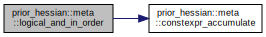
\includegraphics[width=338pt]{namespaceprior__hessian_1_1meta_add11951e7edc2c231ca52c32ac0ee07b_cgraph}
\end{center}
\end{figure}




Here is the caller graph for this function\+:\nopagebreak
\begin{figure}[H]
\begin{center}
\leavevmode
\includegraphics[width=350pt]{namespaceprior__hessian_1_1meta_add11951e7edc2c231ca52c32ac0ee07b_icgraph}
\end{center}
\end{figure}


\index{prior\+\_\+hessian\+::meta@{prior\+\_\+hessian\+::meta}!prod\+\_\+in\+\_\+order@{prod\+\_\+in\+\_\+order}}
\index{prod\+\_\+in\+\_\+order@{prod\+\_\+in\+\_\+order}!prior\+\_\+hessian\+::meta@{prior\+\_\+hessian\+::meta}}
\paragraph[{\texorpdfstring{prod\+\_\+in\+\_\+order(std\+::initializer\+\_\+list$<$ T $>$ L)}{prod_in_order(std::initializer_list< T > L)}}]{\setlength{\rightskip}{0pt plus 5cm}template$<$class T $>$ {\bf P\+R\+I\+O\+R\+\_\+\+H\+E\+S\+S\+I\+A\+N\+\_\+\+M\+E\+T\+A\+\_\+\+C\+O\+N\+S\+T\+E\+X\+PR} T prior\+\_\+hessian\+::meta\+::prod\+\_\+in\+\_\+order (
\begin{DoxyParamCaption}
\item[{std\+::initializer\+\_\+list$<$ T $>$}]{L}
\end{DoxyParamCaption}
)}\hypertarget{namespaceprior__hessian_1_1meta_a32068030d513a09bf78340f87be83639}{}\label{namespaceprior__hessian_1_1meta_a32068030d513a09bf78340f87be83639}


Definition at line 63 of file Meta.\+h.



References constexpr\+\_\+accumulate().



Here is the call graph for this function\+:\nopagebreak
\begin{figure}[H]
\begin{center}
\leavevmode
\includegraphics[width=327pt]{namespaceprior__hessian_1_1meta_a32068030d513a09bf78340f87be83639_cgraph}
\end{center}
\end{figure}


\index{prior\+\_\+hessian\+::meta@{prior\+\_\+hessian\+::meta}!sum\+\_\+in\+\_\+order@{sum\+\_\+in\+\_\+order}}
\index{sum\+\_\+in\+\_\+order@{sum\+\_\+in\+\_\+order}!prior\+\_\+hessian\+::meta@{prior\+\_\+hessian\+::meta}}
\paragraph[{\texorpdfstring{sum\+\_\+in\+\_\+order(std\+::initializer\+\_\+list$<$ T $>$ L)}{sum_in_order(std::initializer_list< T > L)}}]{\setlength{\rightskip}{0pt plus 5cm}template$<$class T $>$ {\bf P\+R\+I\+O\+R\+\_\+\+H\+E\+S\+S\+I\+A\+N\+\_\+\+M\+E\+T\+A\+\_\+\+C\+O\+N\+S\+T\+E\+X\+PR} T prior\+\_\+hessian\+::meta\+::sum\+\_\+in\+\_\+order (
\begin{DoxyParamCaption}
\item[{std\+::initializer\+\_\+list$<$ T $>$}]{L}
\end{DoxyParamCaption}
)}\hypertarget{namespaceprior__hessian_1_1meta_ab09470f06d05f5c58e249a03ef19242f}{}\label{namespaceprior__hessian_1_1meta_ab09470f06d05f5c58e249a03ef19242f}


Definition at line 58 of file Meta.\+h.



References constexpr\+\_\+accumulate(), and P\+R\+I\+O\+R\+\_\+\+H\+E\+S\+S\+I\+A\+N\+\_\+\+M\+E\+T\+A\+\_\+\+C\+O\+N\+S\+T\+E\+X\+PR.



Referenced by prior\+\_\+hessian\+::\+Copula\+Dist\+Impl\+::\+Copula\+Dist$<$ Copula\+Template, Marginal\+Dist\+Ts $>$\+::operator!=().



Here is the call graph for this function\+:\nopagebreak
\begin{figure}[H]
\begin{center}
\leavevmode
\includegraphics[width=327pt]{namespaceprior__hessian_1_1meta_ab09470f06d05f5c58e249a03ef19242f_cgraph}
\end{center}
\end{figure}




Here is the caller graph for this function\+:\nopagebreak
\begin{figure}[H]
\begin{center}
\leavevmode
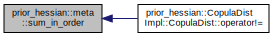
\includegraphics[width=345pt]{namespaceprior__hessian_1_1meta_ab09470f06d05f5c58e249a03ef19242f_icgraph}
\end{center}
\end{figure}



\hypertarget{namespaceprior__hessian_1_1polylog}{}\subsection{prior\+\_\+hessian\+:\+:polylog Namespace Reference}
\label{namespaceprior__hessian_1_1polylog}\index{prior\+\_\+hessian\+::polylog@{prior\+\_\+hessian\+::polylog}}
\subsubsection*{Functions}
\begin{DoxyCompactItemize}
\item 
{\footnotesize template$<$int n$>$ }\\double \hyperlink{namespaceprior__hessian_1_1polylog_a329ad31f0b2ebd507f969067103adea7}{eulerian\+\_\+polynomial} (double z)
\item 
{\footnotesize template$<$$>$ }\\double \hyperlink{namespaceprior__hessian_1_1polylog_aa691a3272d02cfb22cf9bbfe6d37131e}{eulerian\+\_\+polynomial$<$ 0 $>$} (double)
\item 
{\footnotesize template$<$$>$ }\\double \hyperlink{namespaceprior__hessian_1_1polylog_a7e9bf19ef60fa1e7c17ac6ffbb8cd5bd}{eulerian\+\_\+polynomial$<$ 1 $>$} (double z)
\item 
{\footnotesize template$<$$>$ }\\double \hyperlink{namespaceprior__hessian_1_1polylog_a79c383d1be5bf5da28e8735c1deadc31}{eulerian\+\_\+polynomial$<$ 2 $>$} (double z)
\item 
{\footnotesize template$<$$>$ }\\double \hyperlink{namespaceprior__hessian_1_1polylog_aa63cfe2d87dc42a0c1b9bae049759d8d}{eulerian\+\_\+polynomial$<$ 3 $>$} (double z)
\item 
{\footnotesize template$<$$>$ }\\double \hyperlink{namespaceprior__hessian_1_1polylog_a7c0eabb95ea5409645a5c6a1e634d8d0}{eulerian\+\_\+polynomial$<$ 4 $>$} (double z)
\item 
{\footnotesize template$<$$>$ }\\double \hyperlink{namespaceprior__hessian_1_1polylog_af257c6bed7aba2638d0bfc8f0eb2f391}{eulerian\+\_\+polynomial$<$ 5 $>$} (double z)
\item 
{\footnotesize template$<$$>$ }\\double \hyperlink{namespaceprior__hessian_1_1polylog_aa4f73b479dce7efface0d52a49efc6e4}{eulerian\+\_\+polynomial$<$ 6 $>$} (double z)
\item 
{\footnotesize template$<$$>$ }\\double \hyperlink{namespaceprior__hessian_1_1polylog_aa20c9f45040c2b0da1e271208a9fd1f2}{eulerian\+\_\+polynomial$<$ 7 $>$} (double z)
\item 
{\footnotesize template$<$$>$ }\\double \hyperlink{namespaceprior__hessian_1_1polylog_a70bec6b8961ab8a62d9b8b96edd5e639}{eulerian\+\_\+polynomial$<$ 8 $>$} (double z)
\item 
{\footnotesize template$<$$>$ }\\double \hyperlink{namespaceprior__hessian_1_1polylog_a91e8397a4e38129284f72cb4ff0fd1a7}{eulerian\+\_\+polynomial$<$ 9 $>$} (double z)
\item 
{\footnotesize template$<$int n$>$ }\\double \hyperlink{namespaceprior__hessian_1_1polylog_abb5fc2ad3b1509f49ea4b2fc05d916bb}{polylog} (double z)
\item 
{\footnotesize template$<$$>$ }\\double \hyperlink{namespaceprior__hessian_1_1polylog_a461e69d75c8338b404b3b5261b1ab626}{polylog$<$ 1 $>$} (double z)
\end{DoxyCompactItemize}


\subsubsection{Function Documentation}
\index{prior\+\_\+hessian\+::polylog@{prior\+\_\+hessian\+::polylog}!eulerian\+\_\+polynomial@{eulerian\+\_\+polynomial}}
\index{eulerian\+\_\+polynomial@{eulerian\+\_\+polynomial}!prior\+\_\+hessian\+::polylog@{prior\+\_\+hessian\+::polylog}}
\paragraph[{\texorpdfstring{eulerian\+\_\+polynomial(double z)}{eulerian_polynomial(double z)}}]{\setlength{\rightskip}{0pt plus 5cm}template$<$int n$>$ double prior\+\_\+hessian\+::polylog\+::eulerian\+\_\+polynomial (
\begin{DoxyParamCaption}
\item[{double}]{z}
\end{DoxyParamCaption}
)}\hypertarget{namespaceprior__hessian_1_1polylog_a329ad31f0b2ebd507f969067103adea7}{}\label{namespaceprior__hessian_1_1polylog_a329ad31f0b2ebd507f969067103adea7}
\index{prior\+\_\+hessian\+::polylog@{prior\+\_\+hessian\+::polylog}!eulerian\+\_\+polynomial$<$ 0 $>$@{eulerian\+\_\+polynomial$<$ 0 $>$}}
\index{eulerian\+\_\+polynomial$<$ 0 $>$@{eulerian\+\_\+polynomial$<$ 0 $>$}!prior\+\_\+hessian\+::polylog@{prior\+\_\+hessian\+::polylog}}
\paragraph[{\texorpdfstring{eulerian\+\_\+polynomial$<$ 0 $>$(double)}{eulerian_polynomial< 0 >(double)}}]{\setlength{\rightskip}{0pt plus 5cm}template$<$$>$ double {\bf prior\+\_\+hessian\+::polylog\+::eulerian\+\_\+polynomial}$<$ 0 $>$ (
\begin{DoxyParamCaption}
\item[{double}]{}
\end{DoxyParamCaption}
)}\hypertarget{namespaceprior__hessian_1_1polylog_aa691a3272d02cfb22cf9bbfe6d37131e}{}\label{namespaceprior__hessian_1_1polylog_aa691a3272d02cfb22cf9bbfe6d37131e}


Definition at line 17 of file Poly\+Log.\+h.

\index{prior\+\_\+hessian\+::polylog@{prior\+\_\+hessian\+::polylog}!eulerian\+\_\+polynomial$<$ 1 $>$@{eulerian\+\_\+polynomial$<$ 1 $>$}}
\index{eulerian\+\_\+polynomial$<$ 1 $>$@{eulerian\+\_\+polynomial$<$ 1 $>$}!prior\+\_\+hessian\+::polylog@{prior\+\_\+hessian\+::polylog}}
\paragraph[{\texorpdfstring{eulerian\+\_\+polynomial$<$ 1 $>$(double z)}{eulerian_polynomial< 1 >(double z)}}]{\setlength{\rightskip}{0pt plus 5cm}template$<$$>$ double {\bf prior\+\_\+hessian\+::polylog\+::eulerian\+\_\+polynomial}$<$ 1 $>$ (
\begin{DoxyParamCaption}
\item[{double}]{z}
\end{DoxyParamCaption}
)}\hypertarget{namespaceprior__hessian_1_1polylog_a7e9bf19ef60fa1e7c17ac6ffbb8cd5bd}{}\label{namespaceprior__hessian_1_1polylog_a7e9bf19ef60fa1e7c17ac6ffbb8cd5bd}


Definition at line 23 of file Poly\+Log.\+h.

\index{prior\+\_\+hessian\+::polylog@{prior\+\_\+hessian\+::polylog}!eulerian\+\_\+polynomial$<$ 2 $>$@{eulerian\+\_\+polynomial$<$ 2 $>$}}
\index{eulerian\+\_\+polynomial$<$ 2 $>$@{eulerian\+\_\+polynomial$<$ 2 $>$}!prior\+\_\+hessian\+::polylog@{prior\+\_\+hessian\+::polylog}}
\paragraph[{\texorpdfstring{eulerian\+\_\+polynomial$<$ 2 $>$(double z)}{eulerian_polynomial< 2 >(double z)}}]{\setlength{\rightskip}{0pt plus 5cm}template$<$$>$ double {\bf prior\+\_\+hessian\+::polylog\+::eulerian\+\_\+polynomial}$<$ 2 $>$ (
\begin{DoxyParamCaption}
\item[{double}]{z}
\end{DoxyParamCaption}
)}\hypertarget{namespaceprior__hessian_1_1polylog_a79c383d1be5bf5da28e8735c1deadc31}{}\label{namespaceprior__hessian_1_1polylog_a79c383d1be5bf5da28e8735c1deadc31}


Definition at line 29 of file Poly\+Log.\+h.

\index{prior\+\_\+hessian\+::polylog@{prior\+\_\+hessian\+::polylog}!eulerian\+\_\+polynomial$<$ 3 $>$@{eulerian\+\_\+polynomial$<$ 3 $>$}}
\index{eulerian\+\_\+polynomial$<$ 3 $>$@{eulerian\+\_\+polynomial$<$ 3 $>$}!prior\+\_\+hessian\+::polylog@{prior\+\_\+hessian\+::polylog}}
\paragraph[{\texorpdfstring{eulerian\+\_\+polynomial$<$ 3 $>$(double z)}{eulerian_polynomial< 3 >(double z)}}]{\setlength{\rightskip}{0pt plus 5cm}template$<$$>$ double {\bf prior\+\_\+hessian\+::polylog\+::eulerian\+\_\+polynomial}$<$ 3 $>$ (
\begin{DoxyParamCaption}
\item[{double}]{z}
\end{DoxyParamCaption}
)}\hypertarget{namespaceprior__hessian_1_1polylog_aa63cfe2d87dc42a0c1b9bae049759d8d}{}\label{namespaceprior__hessian_1_1polylog_aa63cfe2d87dc42a0c1b9bae049759d8d}


Definition at line 35 of file Poly\+Log.\+h.

\index{prior\+\_\+hessian\+::polylog@{prior\+\_\+hessian\+::polylog}!eulerian\+\_\+polynomial$<$ 4 $>$@{eulerian\+\_\+polynomial$<$ 4 $>$}}
\index{eulerian\+\_\+polynomial$<$ 4 $>$@{eulerian\+\_\+polynomial$<$ 4 $>$}!prior\+\_\+hessian\+::polylog@{prior\+\_\+hessian\+::polylog}}
\paragraph[{\texorpdfstring{eulerian\+\_\+polynomial$<$ 4 $>$(double z)}{eulerian_polynomial< 4 >(double z)}}]{\setlength{\rightskip}{0pt plus 5cm}template$<$$>$ double {\bf prior\+\_\+hessian\+::polylog\+::eulerian\+\_\+polynomial}$<$ 4 $>$ (
\begin{DoxyParamCaption}
\item[{double}]{z}
\end{DoxyParamCaption}
)}\hypertarget{namespaceprior__hessian_1_1polylog_a7c0eabb95ea5409645a5c6a1e634d8d0}{}\label{namespaceprior__hessian_1_1polylog_a7c0eabb95ea5409645a5c6a1e634d8d0}


Definition at line 41 of file Poly\+Log.\+h.

\index{prior\+\_\+hessian\+::polylog@{prior\+\_\+hessian\+::polylog}!eulerian\+\_\+polynomial$<$ 5 $>$@{eulerian\+\_\+polynomial$<$ 5 $>$}}
\index{eulerian\+\_\+polynomial$<$ 5 $>$@{eulerian\+\_\+polynomial$<$ 5 $>$}!prior\+\_\+hessian\+::polylog@{prior\+\_\+hessian\+::polylog}}
\paragraph[{\texorpdfstring{eulerian\+\_\+polynomial$<$ 5 $>$(double z)}{eulerian_polynomial< 5 >(double z)}}]{\setlength{\rightskip}{0pt plus 5cm}template$<$$>$ double {\bf prior\+\_\+hessian\+::polylog\+::eulerian\+\_\+polynomial}$<$ 5 $>$ (
\begin{DoxyParamCaption}
\item[{double}]{z}
\end{DoxyParamCaption}
)}\hypertarget{namespaceprior__hessian_1_1polylog_af257c6bed7aba2638d0bfc8f0eb2f391}{}\label{namespaceprior__hessian_1_1polylog_af257c6bed7aba2638d0bfc8f0eb2f391}


Definition at line 47 of file Poly\+Log.\+h.

\index{prior\+\_\+hessian\+::polylog@{prior\+\_\+hessian\+::polylog}!eulerian\+\_\+polynomial$<$ 6 $>$@{eulerian\+\_\+polynomial$<$ 6 $>$}}
\index{eulerian\+\_\+polynomial$<$ 6 $>$@{eulerian\+\_\+polynomial$<$ 6 $>$}!prior\+\_\+hessian\+::polylog@{prior\+\_\+hessian\+::polylog}}
\paragraph[{\texorpdfstring{eulerian\+\_\+polynomial$<$ 6 $>$(double z)}{eulerian_polynomial< 6 >(double z)}}]{\setlength{\rightskip}{0pt plus 5cm}template$<$$>$ double {\bf prior\+\_\+hessian\+::polylog\+::eulerian\+\_\+polynomial}$<$ 6 $>$ (
\begin{DoxyParamCaption}
\item[{double}]{z}
\end{DoxyParamCaption}
)}\hypertarget{namespaceprior__hessian_1_1polylog_aa4f73b479dce7efface0d52a49efc6e4}{}\label{namespaceprior__hessian_1_1polylog_aa4f73b479dce7efface0d52a49efc6e4}


Definition at line 53 of file Poly\+Log.\+h.

\index{prior\+\_\+hessian\+::polylog@{prior\+\_\+hessian\+::polylog}!eulerian\+\_\+polynomial$<$ 7 $>$@{eulerian\+\_\+polynomial$<$ 7 $>$}}
\index{eulerian\+\_\+polynomial$<$ 7 $>$@{eulerian\+\_\+polynomial$<$ 7 $>$}!prior\+\_\+hessian\+::polylog@{prior\+\_\+hessian\+::polylog}}
\paragraph[{\texorpdfstring{eulerian\+\_\+polynomial$<$ 7 $>$(double z)}{eulerian_polynomial< 7 >(double z)}}]{\setlength{\rightskip}{0pt plus 5cm}template$<$$>$ double {\bf prior\+\_\+hessian\+::polylog\+::eulerian\+\_\+polynomial}$<$ 7 $>$ (
\begin{DoxyParamCaption}
\item[{double}]{z}
\end{DoxyParamCaption}
)}\hypertarget{namespaceprior__hessian_1_1polylog_aa20c9f45040c2b0da1e271208a9fd1f2}{}\label{namespaceprior__hessian_1_1polylog_aa20c9f45040c2b0da1e271208a9fd1f2}


Definition at line 59 of file Poly\+Log.\+h.

\index{prior\+\_\+hessian\+::polylog@{prior\+\_\+hessian\+::polylog}!eulerian\+\_\+polynomial$<$ 8 $>$@{eulerian\+\_\+polynomial$<$ 8 $>$}}
\index{eulerian\+\_\+polynomial$<$ 8 $>$@{eulerian\+\_\+polynomial$<$ 8 $>$}!prior\+\_\+hessian\+::polylog@{prior\+\_\+hessian\+::polylog}}
\paragraph[{\texorpdfstring{eulerian\+\_\+polynomial$<$ 8 $>$(double z)}{eulerian_polynomial< 8 >(double z)}}]{\setlength{\rightskip}{0pt plus 5cm}template$<$$>$ double {\bf prior\+\_\+hessian\+::polylog\+::eulerian\+\_\+polynomial}$<$ 8 $>$ (
\begin{DoxyParamCaption}
\item[{double}]{z}
\end{DoxyParamCaption}
)}\hypertarget{namespaceprior__hessian_1_1polylog_a70bec6b8961ab8a62d9b8b96edd5e639}{}\label{namespaceprior__hessian_1_1polylog_a70bec6b8961ab8a62d9b8b96edd5e639}


Definition at line 65 of file Poly\+Log.\+h.

\index{prior\+\_\+hessian\+::polylog@{prior\+\_\+hessian\+::polylog}!eulerian\+\_\+polynomial$<$ 9 $>$@{eulerian\+\_\+polynomial$<$ 9 $>$}}
\index{eulerian\+\_\+polynomial$<$ 9 $>$@{eulerian\+\_\+polynomial$<$ 9 $>$}!prior\+\_\+hessian\+::polylog@{prior\+\_\+hessian\+::polylog}}
\paragraph[{\texorpdfstring{eulerian\+\_\+polynomial$<$ 9 $>$(double z)}{eulerian_polynomial< 9 >(double z)}}]{\setlength{\rightskip}{0pt plus 5cm}template$<$$>$ double {\bf prior\+\_\+hessian\+::polylog\+::eulerian\+\_\+polynomial}$<$ 9 $>$ (
\begin{DoxyParamCaption}
\item[{double}]{z}
\end{DoxyParamCaption}
)}\hypertarget{namespaceprior__hessian_1_1polylog_a91e8397a4e38129284f72cb4ff0fd1a7}{}\label{namespaceprior__hessian_1_1polylog_a91e8397a4e38129284f72cb4ff0fd1a7}


Definition at line 70 of file Poly\+Log.\+h.



References polylog().



Here is the call graph for this function\+:\nopagebreak
\begin{figure}[H]
\begin{center}
\leavevmode
\includegraphics[width=348pt]{namespaceprior__hessian_1_1polylog_a91e8397a4e38129284f72cb4ff0fd1a7_cgraph}
\end{center}
\end{figure}


\index{prior\+\_\+hessian\+::polylog@{prior\+\_\+hessian\+::polylog}!polylog@{polylog}}
\index{polylog@{polylog}!prior\+\_\+hessian\+::polylog@{prior\+\_\+hessian\+::polylog}}
\paragraph[{\texorpdfstring{polylog(double z)}{polylog(double z)}}]{\setlength{\rightskip}{0pt plus 5cm}template$<$int n$>$ double prior\+\_\+hessian\+::polylog\+::polylog (
\begin{DoxyParamCaption}
\item[{double}]{z}
\end{DoxyParamCaption}
)}\hypertarget{namespaceprior__hessian_1_1polylog_abb5fc2ad3b1509f49ea4b2fc05d916bb}{}\label{namespaceprior__hessian_1_1polylog_abb5fc2ad3b1509f49ea4b2fc05d916bb}


Referenced by prior\+\_\+hessian\+::\+A\+M\+H\+Copula$<$ Ndim $>$\+::d1\+\_\+igen(), prior\+\_\+hessian\+::\+A\+M\+H\+Copula$<$ Ndim $>$\+::ddim\+\_\+gen(), eulerian\+\_\+polynomial$<$ 9 $>$(), and polylog$<$ 1 $>$().



Here is the caller graph for this function\+:\nopagebreak
\begin{figure}[H]
\begin{center}
\leavevmode
\includegraphics[width=350pt]{namespaceprior__hessian_1_1polylog_abb5fc2ad3b1509f49ea4b2fc05d916bb_icgraph}
\end{center}
\end{figure}


\index{prior\+\_\+hessian\+::polylog@{prior\+\_\+hessian\+::polylog}!polylog$<$ 1 $>$@{polylog$<$ 1 $>$}}
\index{polylog$<$ 1 $>$@{polylog$<$ 1 $>$}!prior\+\_\+hessian\+::polylog@{prior\+\_\+hessian\+::polylog}}
\paragraph[{\texorpdfstring{polylog$<$ 1 $>$(double z)}{polylog< 1 >(double z)}}]{\setlength{\rightskip}{0pt plus 5cm}template$<$$>$ double {\bf prior\+\_\+hessian\+::polylog\+::polylog}$<$ 1 $>$ (
\begin{DoxyParamCaption}
\item[{double}]{z}
\end{DoxyParamCaption}
)}\hypertarget{namespaceprior__hessian_1_1polylog_a461e69d75c8338b404b3b5261b1ab626}{}\label{namespaceprior__hessian_1_1polylog_a461e69d75c8338b404b3b5261b1ab626}


Definition at line 120 of file Poly\+Log.\+h.



References polylog().



Here is the call graph for this function\+:\nopagebreak
\begin{figure}[H]
\begin{center}
\leavevmode
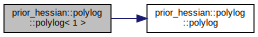
\includegraphics[width=330pt]{namespaceprior__hessian_1_1polylog_a461e69d75c8338b404b3b5261b1ab626_cgraph}
\end{center}
\end{figure}



\section{Class Documentation}
\hypertarget{structprior__hessian_1_1meta_1_1all__dists__are__bounded}{}\subsection{prior\+\_\+hessian\+:\+:meta\+:\+:all\+\_\+dists\+\_\+are\+\_\+bounded$<$ Dist\+Ts $>$ Struct Template Reference}
\label{structprior__hessian_1_1meta_1_1all__dists__are__bounded}\index{prior\+\_\+hessian\+::meta\+::all\+\_\+dists\+\_\+are\+\_\+bounded$<$ Dist\+Ts $>$@{prior\+\_\+hessian\+::meta\+::all\+\_\+dists\+\_\+are\+\_\+bounded$<$ Dist\+Ts $>$}}


{\ttfamily \#include $<$/home/travis/build/markjolah/\+Prior\+Hessian/include/\+Prior\+Hessian/\+Bounds\+Adapted\+Dist.\+h$>$}

\subsubsection*{Static Public Attributes}
\begin{DoxyCompactItemize}
\item 
static constexpr bool \hyperlink{structprior__hessian_1_1meta_1_1all__dists__are__bounded_a2fc2479323836d75b65614a3ee2b640f}{value} = \hyperlink{namespaceprior__hessian_1_1meta_add11951e7edc2c231ca52c32ac0ee07b}{meta\+::logical\+\_\+and\+\_\+in\+\_\+order}(\{\hyperlink{classprior__hessian_1_1detail_1_1dist__adaptor__traits}{detail\+::dist\+\_\+adaptor\+\_\+traits}$<$std\+::decay\+\_\+t$<$Dist\+Ts$>$$>$\+::value...\})
\end{DoxyCompactItemize}


\subsubsection{Detailed Description}
\subsubsection*{template$<$class... Dist\+Ts$>$\\*
struct prior\+\_\+hessian\+::meta\+::all\+\_\+dists\+\_\+are\+\_\+bounded$<$ Dist\+Ts $>$}



Definition at line 81 of file Bounds\+Adapted\+Dist.\+h.



\subsubsection{Member Data Documentation}
\index{prior\+\_\+hessian\+::meta\+::all\+\_\+dists\+\_\+are\+\_\+bounded@{prior\+\_\+hessian\+::meta\+::all\+\_\+dists\+\_\+are\+\_\+bounded}!value@{value}}
\index{value@{value}!prior\+\_\+hessian\+::meta\+::all\+\_\+dists\+\_\+are\+\_\+bounded@{prior\+\_\+hessian\+::meta\+::all\+\_\+dists\+\_\+are\+\_\+bounded}}
\paragraph[{\texorpdfstring{value}{value}}]{\setlength{\rightskip}{0pt plus 5cm}template$<$class... Dist\+Ts$>$ constexpr bool {\bf prior\+\_\+hessian\+::meta\+::all\+\_\+dists\+\_\+are\+\_\+bounded}$<$ Dist\+Ts $>$\+::value = {\bf meta\+::logical\+\_\+and\+\_\+in\+\_\+order}(\{{\bf detail\+::dist\+\_\+adaptor\+\_\+traits}$<$std\+::decay\+\_\+t$<$Dist\+Ts$>$$>$\+::value...\})\hspace{0.3cm}{\ttfamily [static]}}\hypertarget{structprior__hessian_1_1meta_1_1all__dists__are__bounded_a2fc2479323836d75b65614a3ee2b640f}{}\label{structprior__hessian_1_1meta_1_1all__dists__are__bounded_a2fc2479323836d75b65614a3ee2b640f}


Definition at line 83 of file Bounds\+Adapted\+Dist.\+h.



The documentation for this struct was generated from the following file\+:\begin{DoxyCompactItemize}
\item 
\hyperlink{BoundsAdaptedDist_8h}{Bounds\+Adapted\+Dist.\+h}\end{DoxyCompactItemize}

\hypertarget{classprior__hessian_1_1AMHCopula}{}\subsection{prior\+\_\+hessian\+:\+:A\+M\+H\+Copula$<$ Ndim $>$ Class Template Reference}
\label{classprior__hessian_1_1AMHCopula}\index{prior\+\_\+hessian\+::\+A\+M\+H\+Copula$<$ Ndim $>$@{prior\+\_\+hessian\+::\+A\+M\+H\+Copula$<$ Ndim $>$}}


{\ttfamily \#include $<$/home/travis/build/markjolah/\+Prior\+Hessian/include/\+Prior\+Hessian/\+A\+M\+H\+Copula.\+h$>$}



Inheritance diagram for prior\+\_\+hessian\+:\+:A\+M\+H\+Copula$<$ Ndim $>$\+:\nopagebreak
\begin{figure}[H]
\begin{center}
\leavevmode
\includegraphics[width=212pt]{classprior__hessian_1_1AMHCopula__inherit__graph}
\end{center}
\end{figure}


Collaboration diagram for prior\+\_\+hessian\+:\+:A\+M\+H\+Copula$<$ Ndim $>$\+:\nopagebreak
\begin{figure}[H]
\begin{center}
\leavevmode
\includegraphics[width=212pt]{classprior__hessian_1_1AMHCopula__coll__graph}
\end{center}
\end{figure}
\subsubsection*{Public Types}
\begin{DoxyCompactItemize}
\item 
using \hyperlink{classprior__hessian_1_1AMHCopula_aee8626a3e27e52d8bfecc5201808660a}{Ndim\+VecT} = arma\+::\+Col$<$ double $>$\+::fixed$<$ Ndim $>$
\item 
using \hyperlink{classprior__hessian_1_1AMHCopula_a258252a11a49d2c73e19696b2e0e683d}{Ndim\+MatT} = arma\+::\+Mat$<$ double $>$\+::fixed$<$ Ndim, Ndim $>$
\end{DoxyCompactItemize}
\subsubsection*{Public Member Functions}
\begin{DoxyCompactItemize}
\item 
\hyperlink{classprior__hessian_1_1AMHCopula_aea48377467c59f5f882e88f6611a8b56}{A\+M\+H\+Copula} ()
\item 
\hyperlink{classprior__hessian_1_1AMHCopula_a47d4b9c294f1a41069d8991513e81351}{A\+M\+H\+Copula} (double \hyperlink{classprior__hessian_1_1AMHCopula_a11696b4a8cef12a30706cd745820b201}{theta})
\item 
double \hyperlink{classprior__hessian_1_1AMHCopula_a11696b4a8cef12a30706cd745820b201}{theta} () const 
\item 
void \hyperlink{classprior__hessian_1_1AMHCopula_a80bcb09b15bdb3c404f028772932c081}{set\+\_\+theta} (double val)
\item 
bool \hyperlink{classprior__hessian_1_1AMHCopula_a29ff4d88263399c4ee76233644c0de9f}{operator==} (const \hyperlink{classprior__hessian_1_1AMHCopula}{A\+M\+H\+Copula}$<$ Ndim $>$ \&o) const 
\item 
bool \hyperlink{classprior__hessian_1_1AMHCopula_a52be601283a5a2dc619492d74fad860f}{operator!=} (const \hyperlink{classprior__hessian_1_1AMHCopula}{A\+M\+H\+Copula}$<$ Ndim $>$ \&o) const 
\item 
{\footnotesize template$<$class Vec $>$ }\\void \hyperlink{classprior__hessian_1_1AMHCopula_a20cebde68e635d3ad7d0ad67fbcd711e}{set\+\_\+params} (const Vec \&params)
\item 
{\footnotesize template$<$class IterT $>$ }\\void \hyperlink{classprior__hessian_1_1AMHCopula_a244661696f89f48e7466f095c1d3c536}{append\+\_\+params} (IterT \&params)
\item 
{\footnotesize template$<$class IterT $>$ }\\void \hyperlink{classprior__hessian_1_1AMHCopula_a5f5ab047fa0c58b93e7b8e072bc9c682}{set\+\_\+params\+\_\+iter} (IterT \&params)
\item 
{\footnotesize template$<$class Vec $>$ }\\double \hyperlink{classprior__hessian_1_1AMHCopula_aa18585757cb2d4b0723ed80258281278}{cdf} (const Vec \&u) const 
\item 
{\footnotesize template$<$class Vec $>$ }\\double \hyperlink{classprior__hessian_1_1AMHCopula_a8129324c2c30bd4900396198b0c9b957}{pdf} (const Vec \&u) const 
\item 
{\footnotesize template$<$class Vec $>$ }\\double \hyperlink{classprior__hessian_1_1AMHCopula_ad1ce11681554712db7a56bb4cb54c3e9}{llh} (const Vec \&u) const 
\item 
{\footnotesize template$<$class Vec $>$ }\\double \hyperlink{classprior__hessian_1_1AMHCopula_a4c1752aeba875e7ab9563a1a7cd1524b}{rllh} (const Vec \&u) const 
\item 
double \hyperlink{classprior__hessian_1_1AMHCopula_ab0031223c39aec7287cc3cfa3160f6e8}{rllh\+\_\+const} () const 
\item 
{\footnotesize template$<$class Vec $>$ }\\\hyperlink{classprior__hessian_1_1AMHCopula_aee8626a3e27e52d8bfecc5201808660a}{Ndim\+VecT} \hyperlink{classprior__hessian_1_1AMHCopula_a7c3f0e7eb7f4c8eecd37563c35e1f819}{grad} (const Vec \&u) const 
\item 
{\footnotesize template$<$class Vec $>$ }\\\hyperlink{classprior__hessian_1_1AMHCopula_aee8626a3e27e52d8bfecc5201808660a}{Ndim\+VecT} \hyperlink{classprior__hessian_1_1AMHCopula_af87cadcd28d6af3fa8249932f7d01ec7}{grad2} (const Vec \&u) const 
\item 
{\footnotesize template$<$class Vec $>$ }\\\hyperlink{classprior__hessian_1_1AMHCopula_a258252a11a49d2c73e19696b2e0e683d}{Ndim\+MatT} \hyperlink{classprior__hessian_1_1AMHCopula_a324c075c80fb95ed8b69bd601e6a4de6}{hess} (const Vec \&u) const 
\item 
{\footnotesize template$<$class Vec , class Vec2 $>$ }\\void \hyperlink{classprior__hessian_1_1AMHCopula_ad86ca50954d51be0a25a9523f4d7ff5a}{rllh\+\_\+grad\+\_\+accumulate} (const Vec \&u, double \&\hyperlink{classprior__hessian_1_1AMHCopula_a4c1752aeba875e7ab9563a1a7cd1524b}{rllh}, Vec2 \&\hyperlink{classprior__hessian_1_1AMHCopula_a7c3f0e7eb7f4c8eecd37563c35e1f819}{grad}) const 
\item 
{\footnotesize template$<$class Vec , class Vec2 $>$ }\\void \hyperlink{classprior__hessian_1_1AMHCopula_ae6aab20b3c845dfe2dd699df724755eb}{rllh\+\_\+grad\+\_\+grad2\+\_\+accumulate} (const Vec \&u, double \&\hyperlink{classprior__hessian_1_1AMHCopula_a4c1752aeba875e7ab9563a1a7cd1524b}{rllh}, Vec2 \&\hyperlink{classprior__hessian_1_1AMHCopula_a7c3f0e7eb7f4c8eecd37563c35e1f819}{grad}, Vec2 \&\hyperlink{classprior__hessian_1_1AMHCopula_af87cadcd28d6af3fa8249932f7d01ec7}{grad2}) const 
\item 
{\footnotesize template$<$class Vec , class Vec2 , class Mat $>$ }\\void \hyperlink{classprior__hessian_1_1AMHCopula_ab869b33caebfb6ae4e94f180c8f851bb}{rllh\+\_\+grad\+\_\+hess\+\_\+accumulate} (const Vec \&u, double \&\hyperlink{classprior__hessian_1_1AMHCopula_a4c1752aeba875e7ab9563a1a7cd1524b}{rllh}, Vec2 \&\hyperlink{classprior__hessian_1_1AMHCopula_a7c3f0e7eb7f4c8eecd37563c35e1f819}{grad}, Mat \&\hyperlink{classprior__hessian_1_1AMHCopula_a324c075c80fb95ed8b69bd601e6a4de6}{hess}) const 
\item 
{\footnotesize template$<$class RngT $>$ }\\\hyperlink{classprior__hessian_1_1AMHCopula_aee8626a3e27e52d8bfecc5201808660a}{Ndim\+VecT} \hyperlink{classprior__hessian_1_1AMHCopula_a96b5928f1be384c8d0a4efb09b8e49a1}{sample} (RngT \&rng) const 
\item 
double \hyperlink{classprior__hessian_1_1AMHCopula_a2c3506804bb44c972b94cf100404e2c6}{gen} (double t) const 
\item 
double \hyperlink{classprior__hessian_1_1AMHCopula_a9fc68a651139c1c7d28a8144562a09f3}{ddim\+\_\+gen} (double t) const 
\item 
double \hyperlink{classprior__hessian_1_1AMHCopula_a8d5daac3653a101d7068ef9dc0591002}{igen} (double u) const 
\item 
double \hyperlink{classprior__hessian_1_1AMHCopula_a19aecc89d6a1d6c46aa595a13999cfb2}{d1\+\_\+igen} (double u) const 
\item 
{\footnotesize template$<$class Vec $>$ }\\double \hyperlink{classprior__hessian_1_1AMHCopula_a38e091a72ecb8c9df42e88017b2d347e}{igen\+\_\+sum} (const Vec \&u)
\end{DoxyCompactItemize}
\subsubsection*{Static Public Member Functions}
\begin{DoxyCompactItemize}
\item 
static const \hyperlink{namespaceprior__hessian_a61fc0176249462ee94fe3cca92cf3f8c}{String\+VecT} \& \hyperlink{classprior__hessian_1_1AMHCopula_a9982c3f1b0c8c8a44731e162c8783022}{param\+\_\+names} ()
\item 
static constexpr \hyperlink{namespaceprior__hessian_aa8d589f74e88bfa3b5750118acd1ab78}{IdxT} \hyperlink{classprior__hessian_1_1AMHCopula_ade20f55d6cbc96e29988da774b6a7cc0}{num\+\_\+params} ()
\item 
static constexpr \hyperlink{namespaceprior__hessian_aa8d589f74e88bfa3b5750118acd1ab78}{IdxT} \hyperlink{classprior__hessian_1_1AMHCopula_aaacec957c8d8e24df1100aee2694fe3a}{num\+\_\+dim} ()
\item 
static double \hyperlink{classprior__hessian_1_1AMHCopula_ae714c397e21c45b8f57e3ea58659a068}{param\+\_\+lbound} ()
\item 
static double \hyperlink{classprior__hessian_1_1AMHCopula_a7bb6324e170cdc4cc9b1721cd12e99e5}{param\+\_\+ubound} ()
\item 
static bool \hyperlink{classprior__hessian_1_1AMHCopula_a9d4b8453eedea358f829f8d4c911d8c4}{check\+\_\+theta} (double val)
\item 
{\footnotesize template$<$class Vec $>$ }\\static bool \hyperlink{classprior__hessian_1_1AMHCopula_a7052e693079deb29636e505aa37072a5}{check\+\_\+params} (const Vec \&params)
\item 
{\footnotesize template$<$class IterT $>$ }\\static bool \hyperlink{classprior__hessian_1_1AMHCopula_a5878ce4111fcb580ed74d5100aafc37b}{check\+\_\+params\+\_\+iter} (IterT \&params)
\item 
{\footnotesize template$<$class Vec $>$ }\\static void \hyperlink{classprior__hessian_1_1AMHCopula_a8602b8b27ee8b50be3dc979f8b229406}{rllh\+\_\+dtheta\+\_\+accumulate} (double \hyperlink{classprior__hessian_1_1AMHCopula_a11696b4a8cef12a30706cd745820b201}{theta}, const Vec \&u, double \&\hyperlink{classprior__hessian_1_1AMHCopula_a4c1752aeba875e7ab9563a1a7cd1524b}{rllh}, double \&dtheta)
\item 
{\footnotesize template$<$class Vec $>$ }\\static void \hyperlink{classprior__hessian_1_1AMHCopula_aee053f024e655950ad677d53e01d6b4f}{rllh\+\_\+d2theta\+\_\+accumulate} (double \hyperlink{classprior__hessian_1_1AMHCopula_a11696b4a8cef12a30706cd745820b201}{theta}, const Vec \&u, double \&\hyperlink{classprior__hessian_1_1AMHCopula_a4c1752aeba875e7ab9563a1a7cd1524b}{rllh}, double \&dtheta, double \&d2theta)
\end{DoxyCompactItemize}


\subsubsection{Detailed Description}
\subsubsection*{template$<$int Ndim$>$\\*
class prior\+\_\+hessian\+::\+A\+M\+H\+Copula$<$ Ndim $>$}



Definition at line 18 of file A\+M\+H\+Copula.\+h.



\subsubsection{Member Typedef Documentation}
\index{prior\+\_\+hessian\+::\+A\+M\+H\+Copula@{prior\+\_\+hessian\+::\+A\+M\+H\+Copula}!Ndim\+MatT@{Ndim\+MatT}}
\index{Ndim\+MatT@{Ndim\+MatT}!prior\+\_\+hessian\+::\+A\+M\+H\+Copula@{prior\+\_\+hessian\+::\+A\+M\+H\+Copula}}
\paragraph[{\texorpdfstring{Ndim\+MatT}{NdimMatT}}]{\setlength{\rightskip}{0pt plus 5cm}template$<$int Ndim$>$ using {\bf prior\+\_\+hessian\+::\+A\+M\+H\+Copula}$<$ Ndim $>$\+::{\bf Ndim\+MatT} =  arma\+::\+Mat$<$double$>$\+::fixed$<$Ndim,Ndim$>$}\hypertarget{classprior__hessian_1_1AMHCopula_a258252a11a49d2c73e19696b2e0e683d}{}\label{classprior__hessian_1_1AMHCopula_a258252a11a49d2c73e19696b2e0e683d}


Definition at line 27 of file A\+M\+H\+Copula.\+h.

\index{prior\+\_\+hessian\+::\+A\+M\+H\+Copula@{prior\+\_\+hessian\+::\+A\+M\+H\+Copula}!Ndim\+VecT@{Ndim\+VecT}}
\index{Ndim\+VecT@{Ndim\+VecT}!prior\+\_\+hessian\+::\+A\+M\+H\+Copula@{prior\+\_\+hessian\+::\+A\+M\+H\+Copula}}
\paragraph[{\texorpdfstring{Ndim\+VecT}{NdimVecT}}]{\setlength{\rightskip}{0pt plus 5cm}template$<$int Ndim$>$ using {\bf prior\+\_\+hessian\+::\+A\+M\+H\+Copula}$<$ Ndim $>$\+::{\bf Ndim\+VecT} =  arma\+::\+Col$<$double$>$\+::fixed$<$Ndim$>$}\hypertarget{classprior__hessian_1_1AMHCopula_aee8626a3e27e52d8bfecc5201808660a}{}\label{classprior__hessian_1_1AMHCopula_aee8626a3e27e52d8bfecc5201808660a}


Definition at line 26 of file A\+M\+H\+Copula.\+h.



\subsubsection{Constructor \& Destructor Documentation}
\index{prior\+\_\+hessian\+::\+A\+M\+H\+Copula@{prior\+\_\+hessian\+::\+A\+M\+H\+Copula}!A\+M\+H\+Copula@{A\+M\+H\+Copula}}
\index{A\+M\+H\+Copula@{A\+M\+H\+Copula}!prior\+\_\+hessian\+::\+A\+M\+H\+Copula@{prior\+\_\+hessian\+::\+A\+M\+H\+Copula}}
\paragraph[{\texorpdfstring{A\+M\+H\+Copula()}{AMHCopula()}}]{\setlength{\rightskip}{0pt plus 5cm}template$<$int Ndim$>$ {\bf prior\+\_\+hessian\+::\+A\+M\+H\+Copula}$<$ Ndim $>$\+::{\bf A\+M\+H\+Copula} (
\begin{DoxyParamCaption}
{}
\end{DoxyParamCaption}
)\hspace{0.3cm}{\ttfamily [inline]}}\hypertarget{classprior__hessian_1_1AMHCopula_aea48377467c59f5f882e88f6611a8b56}{}\label{classprior__hessian_1_1AMHCopula_aea48377467c59f5f882e88f6611a8b56}


Definition at line 35 of file A\+M\+H\+Copula.\+h.



References prior\+\_\+hessian\+::\+A\+M\+H\+Copula$<$ Ndim $>$\+::theta().



Here is the call graph for this function\+:\nopagebreak
\begin{figure}[H]
\begin{center}
\leavevmode
\includegraphics[width=350pt]{classprior__hessian_1_1AMHCopula_aea48377467c59f5f882e88f6611a8b56_cgraph}
\end{center}
\end{figure}


\index{prior\+\_\+hessian\+::\+A\+M\+H\+Copula@{prior\+\_\+hessian\+::\+A\+M\+H\+Copula}!A\+M\+H\+Copula@{A\+M\+H\+Copula}}
\index{A\+M\+H\+Copula@{A\+M\+H\+Copula}!prior\+\_\+hessian\+::\+A\+M\+H\+Copula@{prior\+\_\+hessian\+::\+A\+M\+H\+Copula}}
\paragraph[{\texorpdfstring{A\+M\+H\+Copula(double theta)}{AMHCopula(double theta)}}]{\setlength{\rightskip}{0pt plus 5cm}template$<$int Ndim$>$ {\bf prior\+\_\+hessian\+::\+A\+M\+H\+Copula}$<$ Ndim $>$\+::{\bf A\+M\+H\+Copula} (
\begin{DoxyParamCaption}
\item[{double}]{theta}
\end{DoxyParamCaption}
)}\hypertarget{classprior__hessian_1_1AMHCopula_a47d4b9c294f1a41069d8991513e81351}{}\label{classprior__hessian_1_1AMHCopula_a47d4b9c294f1a41069d8991513e81351}


Definition at line 169 of file A\+M\+H\+Copula.\+h.



References prior\+\_\+hessian\+::\+A\+M\+H\+Copula$<$ Ndim $>$\+::set\+\_\+theta().



Here is the call graph for this function\+:\nopagebreak
\begin{figure}[H]
\begin{center}
\leavevmode
\includegraphics[width=350pt]{classprior__hessian_1_1AMHCopula_a47d4b9c294f1a41069d8991513e81351_cgraph}
\end{center}
\end{figure}




\subsubsection{Member Function Documentation}
\index{prior\+\_\+hessian\+::\+A\+M\+H\+Copula@{prior\+\_\+hessian\+::\+A\+M\+H\+Copula}!append\+\_\+params@{append\+\_\+params}}
\index{append\+\_\+params@{append\+\_\+params}!prior\+\_\+hessian\+::\+A\+M\+H\+Copula@{prior\+\_\+hessian\+::\+A\+M\+H\+Copula}}
\paragraph[{\texorpdfstring{append\+\_\+params(\+Iter\+T \&params)}{append_params(IterT &params)}}]{\setlength{\rightskip}{0pt plus 5cm}template$<$int Ndim$>$ template$<$class IterT $>$ void {\bf prior\+\_\+hessian\+::\+A\+M\+H\+Copula}$<$ Ndim $>$\+::append\+\_\+params (
\begin{DoxyParamCaption}
\item[{IterT \&}]{params}
\end{DoxyParamCaption}
)\hspace{0.3cm}{\ttfamily [inline]}}\hypertarget{classprior__hessian_1_1AMHCopula_a244661696f89f48e7466f095c1d3c536}{}\label{classprior__hessian_1_1AMHCopula_a244661696f89f48e7466f095c1d3c536}


Definition at line 51 of file A\+M\+H\+Copula.\+h.



References prior\+\_\+hessian\+::\+A\+M\+H\+Copula$<$ Ndim $>$\+::theta().



Here is the call graph for this function\+:\nopagebreak
\begin{figure}[H]
\begin{center}
\leavevmode
\includegraphics[width=350pt]{classprior__hessian_1_1AMHCopula_a244661696f89f48e7466f095c1d3c536_cgraph}
\end{center}
\end{figure}


\index{prior\+\_\+hessian\+::\+A\+M\+H\+Copula@{prior\+\_\+hessian\+::\+A\+M\+H\+Copula}!cdf@{cdf}}
\index{cdf@{cdf}!prior\+\_\+hessian\+::\+A\+M\+H\+Copula@{prior\+\_\+hessian\+::\+A\+M\+H\+Copula}}
\paragraph[{\texorpdfstring{cdf(const Vec \&u) const }{cdf(const Vec &u) const }}]{\setlength{\rightskip}{0pt plus 5cm}template$<$int Ndim$>$ template$<$class Vec $>$ double {\bf prior\+\_\+hessian\+::\+A\+M\+H\+Copula}$<$ Ndim $>$\+::cdf (
\begin{DoxyParamCaption}
\item[{const Vec \&}]{u}
\end{DoxyParamCaption}
) const}\hypertarget{classprior__hessian_1_1AMHCopula_aa18585757cb2d4b0723ed80258281278}{}\label{classprior__hessian_1_1AMHCopula_aa18585757cb2d4b0723ed80258281278}


Definition at line 194 of file A\+M\+H\+Copula.\+h.



References prior\+\_\+hessian\+::\+A\+M\+H\+Copula$<$ Ndim $>$\+::theta().



Referenced by prior\+\_\+hessian\+::\+A\+M\+H\+Copula$<$ Ndim $>$\+::set\+\_\+params\+\_\+iter().



Here is the call graph for this function\+:\nopagebreak
\begin{figure}[H]
\begin{center}
\leavevmode
\includegraphics[width=350pt]{classprior__hessian_1_1AMHCopula_aa18585757cb2d4b0723ed80258281278_cgraph}
\end{center}
\end{figure}




Here is the caller graph for this function\+:\nopagebreak
\begin{figure}[H]
\begin{center}
\leavevmode
\includegraphics[width=350pt]{classprior__hessian_1_1AMHCopula_aa18585757cb2d4b0723ed80258281278_icgraph}
\end{center}
\end{figure}


\index{prior\+\_\+hessian\+::\+A\+M\+H\+Copula@{prior\+\_\+hessian\+::\+A\+M\+H\+Copula}!check\+\_\+params@{check\+\_\+params}}
\index{check\+\_\+params@{check\+\_\+params}!prior\+\_\+hessian\+::\+A\+M\+H\+Copula@{prior\+\_\+hessian\+::\+A\+M\+H\+Copula}}
\paragraph[{\texorpdfstring{check\+\_\+params(const Vec \&params)}{check_params(const Vec &params)}}]{\setlength{\rightskip}{0pt plus 5cm}template$<$int Ndim$>$ template$<$class Vec $>$ static bool {\bf prior\+\_\+hessian\+::\+A\+M\+H\+Copula}$<$ Ndim $>$\+::check\+\_\+params (
\begin{DoxyParamCaption}
\item[{const Vec \&}]{params}
\end{DoxyParamCaption}
)\hspace{0.3cm}{\ttfamily [inline]}, {\ttfamily [static]}}\hypertarget{classprior__hessian_1_1AMHCopula_a7052e693079deb29636e505aa37072a5}{}\label{classprior__hessian_1_1AMHCopula_a7052e693079deb29636e505aa37072a5}


Definition at line 45 of file A\+M\+H\+Copula.\+h.



References prior\+\_\+hessian\+::\+A\+M\+H\+Copula$<$ Ndim $>$\+::check\+\_\+theta().



Here is the call graph for this function\+:\nopagebreak
\begin{figure}[H]
\begin{center}
\leavevmode
\includegraphics[width=350pt]{classprior__hessian_1_1AMHCopula_a7052e693079deb29636e505aa37072a5_cgraph}
\end{center}
\end{figure}


\index{prior\+\_\+hessian\+::\+A\+M\+H\+Copula@{prior\+\_\+hessian\+::\+A\+M\+H\+Copula}!check\+\_\+params\+\_\+iter@{check\+\_\+params\+\_\+iter}}
\index{check\+\_\+params\+\_\+iter@{check\+\_\+params\+\_\+iter}!prior\+\_\+hessian\+::\+A\+M\+H\+Copula@{prior\+\_\+hessian\+::\+A\+M\+H\+Copula}}
\paragraph[{\texorpdfstring{check\+\_\+params\+\_\+iter(\+Iter\+T \&params)}{check_params_iter(IterT &params)}}]{\setlength{\rightskip}{0pt plus 5cm}template$<$int Ndim$>$ template$<$class IterT $>$ static bool {\bf prior\+\_\+hessian\+::\+A\+M\+H\+Copula}$<$ Ndim $>$\+::check\+\_\+params\+\_\+iter (
\begin{DoxyParamCaption}
\item[{IterT \&}]{params}
\end{DoxyParamCaption}
)\hspace{0.3cm}{\ttfamily [inline]}, {\ttfamily [static]}}\hypertarget{classprior__hessian_1_1AMHCopula_a5878ce4111fcb580ed74d5100aafc37b}{}\label{classprior__hessian_1_1AMHCopula_a5878ce4111fcb580ed74d5100aafc37b}


Definition at line 49 of file A\+M\+H\+Copula.\+h.



References prior\+\_\+hessian\+::\+A\+M\+H\+Copula$<$ Ndim $>$\+::check\+\_\+theta().



Here is the call graph for this function\+:\nopagebreak
\begin{figure}[H]
\begin{center}
\leavevmode
\includegraphics[width=350pt]{classprior__hessian_1_1AMHCopula_a5878ce4111fcb580ed74d5100aafc37b_cgraph}
\end{center}
\end{figure}


\index{prior\+\_\+hessian\+::\+A\+M\+H\+Copula@{prior\+\_\+hessian\+::\+A\+M\+H\+Copula}!check\+\_\+theta@{check\+\_\+theta}}
\index{check\+\_\+theta@{check\+\_\+theta}!prior\+\_\+hessian\+::\+A\+M\+H\+Copula@{prior\+\_\+hessian\+::\+A\+M\+H\+Copula}}
\paragraph[{\texorpdfstring{check\+\_\+theta(double val)}{check_theta(double val)}}]{\setlength{\rightskip}{0pt plus 5cm}template$<$int Ndim$>$ bool {\bf prior\+\_\+hessian\+::\+A\+M\+H\+Copula}$<$ Ndim $>$\+::check\+\_\+theta (
\begin{DoxyParamCaption}
\item[{double}]{val}
\end{DoxyParamCaption}
)\hspace{0.3cm}{\ttfamily [static]}}\hypertarget{classprior__hessian_1_1AMHCopula_a9d4b8453eedea358f829f8d4c911d8c4}{}\label{classprior__hessian_1_1AMHCopula_a9d4b8453eedea358f829f8d4c911d8c4}


Definition at line 163 of file A\+M\+H\+Copula.\+h.



Referenced by prior\+\_\+hessian\+::\+A\+M\+H\+Copula$<$ Ndim $>$\+::check\+\_\+params(), prior\+\_\+hessian\+::\+A\+M\+H\+Copula$<$ Ndim $>$\+::check\+\_\+params\+\_\+iter(), prior\+\_\+hessian\+::\+A\+M\+H\+Copula$<$ Ndim $>$\+::param\+\_\+ubound(), and prior\+\_\+hessian\+::\+A\+M\+H\+Copula$<$ Ndim $>$\+::set\+\_\+theta().



Here is the caller graph for this function\+:\nopagebreak
\begin{figure}[H]
\begin{center}
\leavevmode
\includegraphics[width=350pt]{classprior__hessian_1_1AMHCopula_a9d4b8453eedea358f829f8d4c911d8c4_icgraph}
\end{center}
\end{figure}


\index{prior\+\_\+hessian\+::\+A\+M\+H\+Copula@{prior\+\_\+hessian\+::\+A\+M\+H\+Copula}!d1\+\_\+igen@{d1\+\_\+igen}}
\index{d1\+\_\+igen@{d1\+\_\+igen}!prior\+\_\+hessian\+::\+A\+M\+H\+Copula@{prior\+\_\+hessian\+::\+A\+M\+H\+Copula}}
\paragraph[{\texorpdfstring{d1\+\_\+igen(double u) const }{d1_igen(double u) const }}]{\setlength{\rightskip}{0pt plus 5cm}template$<$int Ndim$>$ double {\bf prior\+\_\+hessian\+::\+A\+M\+H\+Copula}$<$ Ndim $>$\+::d1\+\_\+igen (
\begin{DoxyParamCaption}
\item[{double}]{u}
\end{DoxyParamCaption}
) const}\hypertarget{classprior__hessian_1_1AMHCopula_a19aecc89d6a1d6c46aa595a13999cfb2}{}\label{classprior__hessian_1_1AMHCopula_a19aecc89d6a1d6c46aa595a13999cfb2}


Definition at line 284 of file A\+M\+H\+Copula.\+h.



References prior\+\_\+hessian\+::\+A\+M\+H\+Copula$<$ Ndim $>$\+::igen\+\_\+sum(), prior\+\_\+hessian\+::\+A\+M\+H\+Copula$<$ Ndim $>$\+::num\+\_\+dim(), prior\+\_\+hessian\+::polylog\+::polylog(), and prior\+\_\+hessian\+::\+A\+M\+H\+Copula$<$ Ndim $>$\+::theta().



Referenced by prior\+\_\+hessian\+::\+A\+M\+H\+Copula$<$ Ndim $>$\+::llh(), and prior\+\_\+hessian\+::\+A\+M\+H\+Copula$<$ Ndim $>$\+::set\+\_\+params\+\_\+iter().



Here is the call graph for this function\+:\nopagebreak
\begin{figure}[H]
\begin{center}
\leavevmode
\includegraphics[width=350pt]{classprior__hessian_1_1AMHCopula_a19aecc89d6a1d6c46aa595a13999cfb2_cgraph}
\end{center}
\end{figure}




Here is the caller graph for this function\+:\nopagebreak
\begin{figure}[H]
\begin{center}
\leavevmode
\includegraphics[width=350pt]{classprior__hessian_1_1AMHCopula_a19aecc89d6a1d6c46aa595a13999cfb2_icgraph}
\end{center}
\end{figure}


\index{prior\+\_\+hessian\+::\+A\+M\+H\+Copula@{prior\+\_\+hessian\+::\+A\+M\+H\+Copula}!ddim\+\_\+gen@{ddim\+\_\+gen}}
\index{ddim\+\_\+gen@{ddim\+\_\+gen}!prior\+\_\+hessian\+::\+A\+M\+H\+Copula@{prior\+\_\+hessian\+::\+A\+M\+H\+Copula}}
\paragraph[{\texorpdfstring{ddim\+\_\+gen(double t) const }{ddim_gen(double t) const }}]{\setlength{\rightskip}{0pt plus 5cm}template$<$int Ndim$>$ double {\bf prior\+\_\+hessian\+::\+A\+M\+H\+Copula}$<$ Ndim $>$\+::ddim\+\_\+gen (
\begin{DoxyParamCaption}
\item[{double}]{t}
\end{DoxyParamCaption}
) const}\hypertarget{classprior__hessian_1_1AMHCopula_a9fc68a651139c1c7d28a8144562a09f3}{}\label{classprior__hessian_1_1AMHCopula_a9fc68a651139c1c7d28a8144562a09f3}


Definition at line 270 of file A\+M\+H\+Copula.\+h.



References prior\+\_\+hessian\+::\+A\+M\+H\+Copula$<$ Ndim $>$\+::num\+\_\+dim(), and prior\+\_\+hessian\+::polylog\+::polylog().



Referenced by prior\+\_\+hessian\+::\+A\+M\+H\+Copula$<$ Ndim $>$\+::llh(), and prior\+\_\+hessian\+::\+A\+M\+H\+Copula$<$ Ndim $>$\+::set\+\_\+params\+\_\+iter().



Here is the call graph for this function\+:\nopagebreak
\begin{figure}[H]
\begin{center}
\leavevmode
\includegraphics[width=350pt]{classprior__hessian_1_1AMHCopula_a9fc68a651139c1c7d28a8144562a09f3_cgraph}
\end{center}
\end{figure}




Here is the caller graph for this function\+:\nopagebreak
\begin{figure}[H]
\begin{center}
\leavevmode
\includegraphics[width=350pt]{classprior__hessian_1_1AMHCopula_a9fc68a651139c1c7d28a8144562a09f3_icgraph}
\end{center}
\end{figure}


\index{prior\+\_\+hessian\+::\+A\+M\+H\+Copula@{prior\+\_\+hessian\+::\+A\+M\+H\+Copula}!gen@{gen}}
\index{gen@{gen}!prior\+\_\+hessian\+::\+A\+M\+H\+Copula@{prior\+\_\+hessian\+::\+A\+M\+H\+Copula}}
\paragraph[{\texorpdfstring{gen(double t) const }{gen(double t) const }}]{\setlength{\rightskip}{0pt plus 5cm}template$<$int Ndim$>$ double {\bf prior\+\_\+hessian\+::\+A\+M\+H\+Copula}$<$ Ndim $>$\+::gen (
\begin{DoxyParamCaption}
\item[{double}]{t}
\end{DoxyParamCaption}
) const}\hypertarget{classprior__hessian_1_1AMHCopula_a2c3506804bb44c972b94cf100404e2c6}{}\label{classprior__hessian_1_1AMHCopula_a2c3506804bb44c972b94cf100404e2c6}


Definition at line 265 of file A\+M\+H\+Copula.\+h.



Referenced by prior\+\_\+hessian\+::\+A\+M\+H\+Copula$<$ Ndim $>$\+::set\+\_\+params\+\_\+iter().



Here is the caller graph for this function\+:\nopagebreak
\begin{figure}[H]
\begin{center}
\leavevmode
\includegraphics[width=350pt]{classprior__hessian_1_1AMHCopula_a2c3506804bb44c972b94cf100404e2c6_icgraph}
\end{center}
\end{figure}


\index{prior\+\_\+hessian\+::\+A\+M\+H\+Copula@{prior\+\_\+hessian\+::\+A\+M\+H\+Copula}!grad@{grad}}
\index{grad@{grad}!prior\+\_\+hessian\+::\+A\+M\+H\+Copula@{prior\+\_\+hessian\+::\+A\+M\+H\+Copula}}
\paragraph[{\texorpdfstring{grad(const Vec \&u) const }{grad(const Vec &u) const }}]{\setlength{\rightskip}{0pt plus 5cm}template$<$int Ndim$>$ template$<$class Vec $>$ {\bf A\+M\+H\+Copula}$<$ Ndim $>$\+::{\bf Ndim\+VecT} {\bf prior\+\_\+hessian\+::\+A\+M\+H\+Copula}$<$ Ndim $>$\+::grad (
\begin{DoxyParamCaption}
\item[{const Vec \&}]{u}
\end{DoxyParamCaption}
) const}\hypertarget{classprior__hessian_1_1AMHCopula_a7c3f0e7eb7f4c8eecd37563c35e1f819}{}\label{classprior__hessian_1_1AMHCopula_a7c3f0e7eb7f4c8eecd37563c35e1f819}


Definition at line 220 of file A\+M\+H\+Copula.\+h.



References prior\+\_\+hessian\+::\+A\+M\+H\+Copula$<$ Ndim $>$\+::grad2(), and prior\+\_\+hessian\+::\+A\+M\+H\+Copula$<$ Ndim $>$\+::theta().



Referenced by prior\+\_\+hessian\+::\+A\+M\+H\+Copula$<$ Ndim $>$\+::set\+\_\+params\+\_\+iter().



Here is the call graph for this function\+:\nopagebreak
\begin{figure}[H]
\begin{center}
\leavevmode
\includegraphics[width=350pt]{classprior__hessian_1_1AMHCopula_a7c3f0e7eb7f4c8eecd37563c35e1f819_cgraph}
\end{center}
\end{figure}




Here is the caller graph for this function\+:\nopagebreak
\begin{figure}[H]
\begin{center}
\leavevmode
\includegraphics[width=350pt]{classprior__hessian_1_1AMHCopula_a7c3f0e7eb7f4c8eecd37563c35e1f819_icgraph}
\end{center}
\end{figure}


\index{prior\+\_\+hessian\+::\+A\+M\+H\+Copula@{prior\+\_\+hessian\+::\+A\+M\+H\+Copula}!grad2@{grad2}}
\index{grad2@{grad2}!prior\+\_\+hessian\+::\+A\+M\+H\+Copula@{prior\+\_\+hessian\+::\+A\+M\+H\+Copula}}
\paragraph[{\texorpdfstring{grad2(const Vec \&u) const }{grad2(const Vec &u) const }}]{\setlength{\rightskip}{0pt plus 5cm}template$<$int Ndim$>$ template$<$class Vec $>$ {\bf A\+M\+H\+Copula}$<$ Ndim $>$\+::{\bf Ndim\+VecT} {\bf prior\+\_\+hessian\+::\+A\+M\+H\+Copula}$<$ Ndim $>$\+::grad2 (
\begin{DoxyParamCaption}
\item[{const Vec \&}]{u}
\end{DoxyParamCaption}
) const}\hypertarget{classprior__hessian_1_1AMHCopula_af87cadcd28d6af3fa8249932f7d01ec7}{}\label{classprior__hessian_1_1AMHCopula_af87cadcd28d6af3fa8249932f7d01ec7}


Definition at line 234 of file A\+M\+H\+Copula.\+h.



References prior\+\_\+hessian\+::square(), and prior\+\_\+hessian\+::\+A\+M\+H\+Copula$<$ Ndim $>$\+::theta().



Referenced by prior\+\_\+hessian\+::\+A\+M\+H\+Copula$<$ Ndim $>$\+::grad(), and prior\+\_\+hessian\+::\+A\+M\+H\+Copula$<$ Ndim $>$\+::set\+\_\+params\+\_\+iter().



Here is the call graph for this function\+:\nopagebreak
\begin{figure}[H]
\begin{center}
\leavevmode
\includegraphics[width=350pt]{classprior__hessian_1_1AMHCopula_af87cadcd28d6af3fa8249932f7d01ec7_cgraph}
\end{center}
\end{figure}




Here is the caller graph for this function\+:\nopagebreak
\begin{figure}[H]
\begin{center}
\leavevmode
\includegraphics[width=350pt]{classprior__hessian_1_1AMHCopula_af87cadcd28d6af3fa8249932f7d01ec7_icgraph}
\end{center}
\end{figure}


\index{prior\+\_\+hessian\+::\+A\+M\+H\+Copula@{prior\+\_\+hessian\+::\+A\+M\+H\+Copula}!hess@{hess}}
\index{hess@{hess}!prior\+\_\+hessian\+::\+A\+M\+H\+Copula@{prior\+\_\+hessian\+::\+A\+M\+H\+Copula}}
\paragraph[{\texorpdfstring{hess(const Vec \&u) const }{hess(const Vec &u) const }}]{\setlength{\rightskip}{0pt plus 5cm}template$<$int Ndim$>$ template$<$class Vec $>$ {\bf A\+M\+H\+Copula}$<$ Ndim $>$\+::{\bf Ndim\+MatT} {\bf prior\+\_\+hessian\+::\+A\+M\+H\+Copula}$<$ Ndim $>$\+::hess (
\begin{DoxyParamCaption}
\item[{const Vec \&}]{u}
\end{DoxyParamCaption}
) const}\hypertarget{classprior__hessian_1_1AMHCopula_a324c075c80fb95ed8b69bd601e6a4de6}{}\label{classprior__hessian_1_1AMHCopula_a324c075c80fb95ed8b69bd601e6a4de6}


Definition at line 248 of file A\+M\+H\+Copula.\+h.



References prior\+\_\+hessian\+::square(), and prior\+\_\+hessian\+::\+A\+M\+H\+Copula$<$ Ndim $>$\+::theta().



Referenced by prior\+\_\+hessian\+::\+A\+M\+H\+Copula$<$ Ndim $>$\+::set\+\_\+params\+\_\+iter().



Here is the call graph for this function\+:\nopagebreak
\begin{figure}[H]
\begin{center}
\leavevmode
\includegraphics[width=350pt]{classprior__hessian_1_1AMHCopula_a324c075c80fb95ed8b69bd601e6a4de6_cgraph}
\end{center}
\end{figure}




Here is the caller graph for this function\+:\nopagebreak
\begin{figure}[H]
\begin{center}
\leavevmode
\includegraphics[width=350pt]{classprior__hessian_1_1AMHCopula_a324c075c80fb95ed8b69bd601e6a4de6_icgraph}
\end{center}
\end{figure}


\index{prior\+\_\+hessian\+::\+A\+M\+H\+Copula@{prior\+\_\+hessian\+::\+A\+M\+H\+Copula}!igen@{igen}}
\index{igen@{igen}!prior\+\_\+hessian\+::\+A\+M\+H\+Copula@{prior\+\_\+hessian\+::\+A\+M\+H\+Copula}}
\paragraph[{\texorpdfstring{igen(double u) const }{igen(double u) const }}]{\setlength{\rightskip}{0pt plus 5cm}template$<$int Ndim$>$ double {\bf prior\+\_\+hessian\+::\+A\+M\+H\+Copula}$<$ Ndim $>$\+::igen (
\begin{DoxyParamCaption}
\item[{double}]{u}
\end{DoxyParamCaption}
) const}\hypertarget{classprior__hessian_1_1AMHCopula_a8d5daac3653a101d7068ef9dc0591002}{}\label{classprior__hessian_1_1AMHCopula_a8d5daac3653a101d7068ef9dc0591002}


Definition at line 279 of file A\+M\+H\+Copula.\+h.



Referenced by prior\+\_\+hessian\+::\+A\+M\+H\+Copula$<$ Ndim $>$\+::set\+\_\+params\+\_\+iter().



Here is the caller graph for this function\+:\nopagebreak
\begin{figure}[H]
\begin{center}
\leavevmode
\includegraphics[width=350pt]{classprior__hessian_1_1AMHCopula_a8d5daac3653a101d7068ef9dc0591002_icgraph}
\end{center}
\end{figure}


\index{prior\+\_\+hessian\+::\+A\+M\+H\+Copula@{prior\+\_\+hessian\+::\+A\+M\+H\+Copula}!igen\+\_\+sum@{igen\+\_\+sum}}
\index{igen\+\_\+sum@{igen\+\_\+sum}!prior\+\_\+hessian\+::\+A\+M\+H\+Copula@{prior\+\_\+hessian\+::\+A\+M\+H\+Copula}}
\paragraph[{\texorpdfstring{igen\+\_\+sum(const Vec \&u)}{igen_sum(const Vec &u)}}]{\setlength{\rightskip}{0pt plus 5cm}template$<$int Ndim$>$ template$<$class Vec $>$ double {\bf prior\+\_\+hessian\+::\+A\+M\+H\+Copula}$<$ Ndim $>$\+::igen\+\_\+sum (
\begin{DoxyParamCaption}
\item[{const Vec \&}]{u}
\end{DoxyParamCaption}
)\hspace{0.3cm}{\ttfamily [inline]}}\hypertarget{classprior__hessian_1_1AMHCopula_a38e091a72ecb8c9df42e88017b2d347e}{}\label{classprior__hessian_1_1AMHCopula_a38e091a72ecb8c9df42e88017b2d347e}


Definition at line 97 of file A\+M\+H\+Copula.\+h.



References prior\+\_\+hessian\+::\+A\+M\+H\+Copula$<$ Ndim $>$\+::igen\+\_\+sum(), and prior\+\_\+hessian\+::\+A\+M\+H\+Copula$<$ Ndim $>$\+::theta().



Referenced by prior\+\_\+hessian\+::\+A\+M\+H\+Copula$<$ Ndim $>$\+::d1\+\_\+igen(), prior\+\_\+hessian\+::\+A\+M\+H\+Copula$<$ Ndim $>$\+::igen\+\_\+sum(), and prior\+\_\+hessian\+::\+A\+M\+H\+Copula$<$ Ndim $>$\+::llh().



Here is the call graph for this function\+:\nopagebreak
\begin{figure}[H]
\begin{center}
\leavevmode
\includegraphics[width=350pt]{classprior__hessian_1_1AMHCopula_a38e091a72ecb8c9df42e88017b2d347e_cgraph}
\end{center}
\end{figure}




Here is the caller graph for this function\+:\nopagebreak
\begin{figure}[H]
\begin{center}
\leavevmode
\includegraphics[width=350pt]{classprior__hessian_1_1AMHCopula_a38e091a72ecb8c9df42e88017b2d347e_icgraph}
\end{center}
\end{figure}


\index{prior\+\_\+hessian\+::\+A\+M\+H\+Copula@{prior\+\_\+hessian\+::\+A\+M\+H\+Copula}!llh@{llh}}
\index{llh@{llh}!prior\+\_\+hessian\+::\+A\+M\+H\+Copula@{prior\+\_\+hessian\+::\+A\+M\+H\+Copula}}
\paragraph[{\texorpdfstring{llh(const Vec \&u) const }{llh(const Vec &u) const }}]{\setlength{\rightskip}{0pt plus 5cm}template$<$int Ndim$>$ template$<$class Vec $>$ double {\bf prior\+\_\+hessian\+::\+A\+M\+H\+Copula}$<$ Ndim $>$\+::llh (
\begin{DoxyParamCaption}
\item[{const Vec \&}]{u}
\end{DoxyParamCaption}
) const}\hypertarget{classprior__hessian_1_1AMHCopula_ad1ce11681554712db7a56bb4cb54c3e9}{}\label{classprior__hessian_1_1AMHCopula_ad1ce11681554712db7a56bb4cb54c3e9}


Definition at line 210 of file A\+M\+H\+Copula.\+h.



References prior\+\_\+hessian\+::\+A\+M\+H\+Copula$<$ Ndim $>$\+::d1\+\_\+igen(), prior\+\_\+hessian\+::\+A\+M\+H\+Copula$<$ Ndim $>$\+::ddim\+\_\+gen(), and prior\+\_\+hessian\+::\+A\+M\+H\+Copula$<$ Ndim $>$\+::igen\+\_\+sum().



Referenced by prior\+\_\+hessian\+::\+A\+M\+H\+Copula$<$ Ndim $>$\+::set\+\_\+params\+\_\+iter().



Here is the call graph for this function\+:\nopagebreak
\begin{figure}[H]
\begin{center}
\leavevmode
\includegraphics[width=350pt]{classprior__hessian_1_1AMHCopula_ad1ce11681554712db7a56bb4cb54c3e9_cgraph}
\end{center}
\end{figure}




Here is the caller graph for this function\+:\nopagebreak
\begin{figure}[H]
\begin{center}
\leavevmode
\includegraphics[width=350pt]{classprior__hessian_1_1AMHCopula_ad1ce11681554712db7a56bb4cb54c3e9_icgraph}
\end{center}
\end{figure}


\index{prior\+\_\+hessian\+::\+A\+M\+H\+Copula@{prior\+\_\+hessian\+::\+A\+M\+H\+Copula}!num\+\_\+dim@{num\+\_\+dim}}
\index{num\+\_\+dim@{num\+\_\+dim}!prior\+\_\+hessian\+::\+A\+M\+H\+Copula@{prior\+\_\+hessian\+::\+A\+M\+H\+Copula}}
\paragraph[{\texorpdfstring{num\+\_\+dim()}{num_dim()}}]{\setlength{\rightskip}{0pt plus 5cm}template$<$int Ndim$>$ static constexpr {\bf IdxT} {\bf prior\+\_\+hessian\+::\+A\+M\+H\+Copula}$<$ Ndim $>$\+::num\+\_\+dim (
\begin{DoxyParamCaption}
{}
\end{DoxyParamCaption}
)\hspace{0.3cm}{\ttfamily [inline]}, {\ttfamily [static]}}\hypertarget{classprior__hessian_1_1AMHCopula_aaacec957c8d8e24df1100aee2694fe3a}{}\label{classprior__hessian_1_1AMHCopula_aaacec957c8d8e24df1100aee2694fe3a}


Definition at line 30 of file A\+M\+H\+Copula.\+h.



Referenced by prior\+\_\+hessian\+::\+A\+M\+H\+Copula$<$ Ndim $>$\+::d1\+\_\+igen(), and prior\+\_\+hessian\+::\+A\+M\+H\+Copula$<$ Ndim $>$\+::ddim\+\_\+gen().



Here is the caller graph for this function\+:\nopagebreak
\begin{figure}[H]
\begin{center}
\leavevmode
\includegraphics[width=350pt]{classprior__hessian_1_1AMHCopula_aaacec957c8d8e24df1100aee2694fe3a_icgraph}
\end{center}
\end{figure}


\index{prior\+\_\+hessian\+::\+A\+M\+H\+Copula@{prior\+\_\+hessian\+::\+A\+M\+H\+Copula}!num\+\_\+params@{num\+\_\+params}}
\index{num\+\_\+params@{num\+\_\+params}!prior\+\_\+hessian\+::\+A\+M\+H\+Copula@{prior\+\_\+hessian\+::\+A\+M\+H\+Copula}}
\paragraph[{\texorpdfstring{num\+\_\+params()}{num_params()}}]{\setlength{\rightskip}{0pt plus 5cm}template$<$int Ndim$>$ static constexpr {\bf IdxT} {\bf prior\+\_\+hessian\+::\+A\+M\+H\+Copula}$<$ Ndim $>$\+::num\+\_\+params (
\begin{DoxyParamCaption}
{}
\end{DoxyParamCaption}
)\hspace{0.3cm}{\ttfamily [inline]}, {\ttfamily [static]}}\hypertarget{classprior__hessian_1_1AMHCopula_ade20f55d6cbc96e29988da774b6a7cc0}{}\label{classprior__hessian_1_1AMHCopula_ade20f55d6cbc96e29988da774b6a7cc0}


Definition at line 29 of file A\+M\+H\+Copula.\+h.

\index{prior\+\_\+hessian\+::\+A\+M\+H\+Copula@{prior\+\_\+hessian\+::\+A\+M\+H\+Copula}!operator"!=@{operator"!=}}
\index{operator"!=@{operator"!=}!prior\+\_\+hessian\+::\+A\+M\+H\+Copula@{prior\+\_\+hessian\+::\+A\+M\+H\+Copula}}
\paragraph[{\texorpdfstring{operator"!=(const A\+M\+H\+Copula$<$ Ndim $>$ \&o) const }{operator!=(const AMHCopula< Ndim > &o) const }}]{\setlength{\rightskip}{0pt plus 5cm}template$<$int Ndim$>$ bool {\bf prior\+\_\+hessian\+::\+A\+M\+H\+Copula}$<$ Ndim $>$\+::operator!= (
\begin{DoxyParamCaption}
\item[{const {\bf A\+M\+H\+Copula}$<$ Ndim $>$ \&}]{o}
\end{DoxyParamCaption}
) const\hspace{0.3cm}{\ttfamily [inline]}}\hypertarget{classprior__hessian_1_1AMHCopula_a52be601283a5a2dc619492d74fad860f}{}\label{classprior__hessian_1_1AMHCopula_a52be601283a5a2dc619492d74fad860f}


Definition at line 42 of file A\+M\+H\+Copula.\+h.



References prior\+\_\+hessian\+::\+A\+M\+H\+Copula$<$ Ndim $>$\+::theta().



Here is the call graph for this function\+:\nopagebreak
\begin{figure}[H]
\begin{center}
\leavevmode
\includegraphics[width=350pt]{classprior__hessian_1_1AMHCopula_a52be601283a5a2dc619492d74fad860f_cgraph}
\end{center}
\end{figure}


\index{prior\+\_\+hessian\+::\+A\+M\+H\+Copula@{prior\+\_\+hessian\+::\+A\+M\+H\+Copula}!operator==@{operator==}}
\index{operator==@{operator==}!prior\+\_\+hessian\+::\+A\+M\+H\+Copula@{prior\+\_\+hessian\+::\+A\+M\+H\+Copula}}
\paragraph[{\texorpdfstring{operator==(const A\+M\+H\+Copula$<$ Ndim $>$ \&o) const }{operator==(const AMHCopula< Ndim > &o) const }}]{\setlength{\rightskip}{0pt plus 5cm}template$<$int Ndim$>$ bool {\bf prior\+\_\+hessian\+::\+A\+M\+H\+Copula}$<$ Ndim $>$\+::operator== (
\begin{DoxyParamCaption}
\item[{const {\bf A\+M\+H\+Copula}$<$ Ndim $>$ \&}]{o}
\end{DoxyParamCaption}
) const\hspace{0.3cm}{\ttfamily [inline]}}\hypertarget{classprior__hessian_1_1AMHCopula_a29ff4d88263399c4ee76233644c0de9f}{}\label{classprior__hessian_1_1AMHCopula_a29ff4d88263399c4ee76233644c0de9f}


Definition at line 41 of file A\+M\+H\+Copula.\+h.



References prior\+\_\+hessian\+::\+A\+M\+H\+Copula$<$ Ndim $>$\+::theta().



Here is the call graph for this function\+:\nopagebreak
\begin{figure}[H]
\begin{center}
\leavevmode
\includegraphics[width=350pt]{classprior__hessian_1_1AMHCopula_a29ff4d88263399c4ee76233644c0de9f_cgraph}
\end{center}
\end{figure}


\index{prior\+\_\+hessian\+::\+A\+M\+H\+Copula@{prior\+\_\+hessian\+::\+A\+M\+H\+Copula}!param\+\_\+lbound@{param\+\_\+lbound}}
\index{param\+\_\+lbound@{param\+\_\+lbound}!prior\+\_\+hessian\+::\+A\+M\+H\+Copula@{prior\+\_\+hessian\+::\+A\+M\+H\+Copula}}
\paragraph[{\texorpdfstring{param\+\_\+lbound()}{param_lbound()}}]{\setlength{\rightskip}{0pt plus 5cm}template$<$int Ndim$>$ static double {\bf prior\+\_\+hessian\+::\+A\+M\+H\+Copula}$<$ Ndim $>$\+::param\+\_\+lbound (
\begin{DoxyParamCaption}
{}
\end{DoxyParamCaption}
)\hspace{0.3cm}{\ttfamily [inline]}, {\ttfamily [static]}}\hypertarget{classprior__hessian_1_1AMHCopula_ae714c397e21c45b8f57e3ea58659a068}{}\label{classprior__hessian_1_1AMHCopula_ae714c397e21c45b8f57e3ea58659a068}


Definition at line 31 of file A\+M\+H\+Copula.\+h.

\index{prior\+\_\+hessian\+::\+A\+M\+H\+Copula@{prior\+\_\+hessian\+::\+A\+M\+H\+Copula}!param\+\_\+names@{param\+\_\+names}}
\index{param\+\_\+names@{param\+\_\+names}!prior\+\_\+hessian\+::\+A\+M\+H\+Copula@{prior\+\_\+hessian\+::\+A\+M\+H\+Copula}}
\paragraph[{\texorpdfstring{param\+\_\+names()}{param_names()}}]{\setlength{\rightskip}{0pt plus 5cm}template$<$int Ndim$>$ static const {\bf String\+VecT}\& {\bf prior\+\_\+hessian\+::\+A\+M\+H\+Copula}$<$ Ndim $>$\+::param\+\_\+names (
\begin{DoxyParamCaption}
{}
\end{DoxyParamCaption}
)\hspace{0.3cm}{\ttfamily [inline]}, {\ttfamily [static]}}\hypertarget{classprior__hessian_1_1AMHCopula_a9982c3f1b0c8c8a44731e162c8783022}{}\label{classprior__hessian_1_1AMHCopula_a9982c3f1b0c8c8a44731e162c8783022}


Definition at line 28 of file A\+M\+H\+Copula.\+h.

\index{prior\+\_\+hessian\+::\+A\+M\+H\+Copula@{prior\+\_\+hessian\+::\+A\+M\+H\+Copula}!param\+\_\+ubound@{param\+\_\+ubound}}
\index{param\+\_\+ubound@{param\+\_\+ubound}!prior\+\_\+hessian\+::\+A\+M\+H\+Copula@{prior\+\_\+hessian\+::\+A\+M\+H\+Copula}}
\paragraph[{\texorpdfstring{param\+\_\+ubound()}{param_ubound()}}]{\setlength{\rightskip}{0pt plus 5cm}template$<$int Ndim$>$ static double {\bf prior\+\_\+hessian\+::\+A\+M\+H\+Copula}$<$ Ndim $>$\+::param\+\_\+ubound (
\begin{DoxyParamCaption}
{}
\end{DoxyParamCaption}
)\hspace{0.3cm}{\ttfamily [inline]}, {\ttfamily [static]}}\hypertarget{classprior__hessian_1_1AMHCopula_a7bb6324e170cdc4cc9b1721cd12e99e5}{}\label{classprior__hessian_1_1AMHCopula_a7bb6324e170cdc4cc9b1721cd12e99e5}


Definition at line 32 of file A\+M\+H\+Copula.\+h.



References prior\+\_\+hessian\+::\+A\+M\+H\+Copula$<$ Ndim $>$\+::check\+\_\+theta().



Here is the call graph for this function\+:\nopagebreak
\begin{figure}[H]
\begin{center}
\leavevmode
\includegraphics[width=350pt]{classprior__hessian_1_1AMHCopula_a7bb6324e170cdc4cc9b1721cd12e99e5_cgraph}
\end{center}
\end{figure}


\index{prior\+\_\+hessian\+::\+A\+M\+H\+Copula@{prior\+\_\+hessian\+::\+A\+M\+H\+Copula}!pdf@{pdf}}
\index{pdf@{pdf}!prior\+\_\+hessian\+::\+A\+M\+H\+Copula@{prior\+\_\+hessian\+::\+A\+M\+H\+Copula}}
\paragraph[{\texorpdfstring{pdf(const Vec \&u) const }{pdf(const Vec &u) const }}]{\setlength{\rightskip}{0pt plus 5cm}template$<$int Ndim$>$ template$<$class Vec $>$ double {\bf prior\+\_\+hessian\+::\+A\+M\+H\+Copula}$<$ Ndim $>$\+::pdf (
\begin{DoxyParamCaption}
\item[{const Vec \&}]{u}
\end{DoxyParamCaption}
) const}\hypertarget{classprior__hessian_1_1AMHCopula_a8129324c2c30bd4900396198b0c9b957}{}\label{classprior__hessian_1_1AMHCopula_a8129324c2c30bd4900396198b0c9b957}


Definition at line 202 of file A\+M\+H\+Copula.\+h.



References prior\+\_\+hessian\+::\+A\+M\+H\+Copula$<$ Ndim $>$\+::theta().



Referenced by prior\+\_\+hessian\+::\+A\+M\+H\+Copula$<$ Ndim $>$\+::set\+\_\+params\+\_\+iter().



Here is the call graph for this function\+:\nopagebreak
\begin{figure}[H]
\begin{center}
\leavevmode
\includegraphics[width=350pt]{classprior__hessian_1_1AMHCopula_a8129324c2c30bd4900396198b0c9b957_cgraph}
\end{center}
\end{figure}




Here is the caller graph for this function\+:\nopagebreak
\begin{figure}[H]
\begin{center}
\leavevmode
\includegraphics[width=350pt]{classprior__hessian_1_1AMHCopula_a8129324c2c30bd4900396198b0c9b957_icgraph}
\end{center}
\end{figure}


\index{prior\+\_\+hessian\+::\+A\+M\+H\+Copula@{prior\+\_\+hessian\+::\+A\+M\+H\+Copula}!rllh@{rllh}}
\index{rllh@{rllh}!prior\+\_\+hessian\+::\+A\+M\+H\+Copula@{prior\+\_\+hessian\+::\+A\+M\+H\+Copula}}
\paragraph[{\texorpdfstring{rllh(const Vec \&u) const }{rllh(const Vec &u) const }}]{\setlength{\rightskip}{0pt plus 5cm}template$<$int Ndim$>$ template$<$class Vec $>$ double {\bf prior\+\_\+hessian\+::\+A\+M\+H\+Copula}$<$ Ndim $>$\+::rllh (
\begin{DoxyParamCaption}
\item[{const Vec \&}]{u}
\end{DoxyParamCaption}
) const}\hypertarget{classprior__hessian_1_1AMHCopula_a4c1752aeba875e7ab9563a1a7cd1524b}{}\label{classprior__hessian_1_1AMHCopula_a4c1752aeba875e7ab9563a1a7cd1524b}


Referenced by prior\+\_\+hessian\+::\+A\+M\+H\+Copula$<$ Ndim $>$\+::set\+\_\+params\+\_\+iter().



Here is the caller graph for this function\+:\nopagebreak
\begin{figure}[H]
\begin{center}
\leavevmode
\includegraphics[width=350pt]{classprior__hessian_1_1AMHCopula_a4c1752aeba875e7ab9563a1a7cd1524b_icgraph}
\end{center}
\end{figure}


\index{prior\+\_\+hessian\+::\+A\+M\+H\+Copula@{prior\+\_\+hessian\+::\+A\+M\+H\+Copula}!rllh\+\_\+const@{rllh\+\_\+const}}
\index{rllh\+\_\+const@{rllh\+\_\+const}!prior\+\_\+hessian\+::\+A\+M\+H\+Copula@{prior\+\_\+hessian\+::\+A\+M\+H\+Copula}}
\paragraph[{\texorpdfstring{rllh\+\_\+const() const }{rllh_const() const }}]{\setlength{\rightskip}{0pt plus 5cm}template$<$int Ndim$>$ double {\bf prior\+\_\+hessian\+::\+A\+M\+H\+Copula}$<$ Ndim $>$\+::rllh\+\_\+const (
\begin{DoxyParamCaption}
{}
\end{DoxyParamCaption}
) const}\hypertarget{classprior__hessian_1_1AMHCopula_ab0031223c39aec7287cc3cfa3160f6e8}{}\label{classprior__hessian_1_1AMHCopula_ab0031223c39aec7287cc3cfa3160f6e8}


Referenced by prior\+\_\+hessian\+::\+A\+M\+H\+Copula$<$ Ndim $>$\+::set\+\_\+params\+\_\+iter().



Here is the caller graph for this function\+:\nopagebreak
\begin{figure}[H]
\begin{center}
\leavevmode
\includegraphics[width=350pt]{classprior__hessian_1_1AMHCopula_ab0031223c39aec7287cc3cfa3160f6e8_icgraph}
\end{center}
\end{figure}


\index{prior\+\_\+hessian\+::\+A\+M\+H\+Copula@{prior\+\_\+hessian\+::\+A\+M\+H\+Copula}!rllh\+\_\+d2theta\+\_\+accumulate@{rllh\+\_\+d2theta\+\_\+accumulate}}
\index{rllh\+\_\+d2theta\+\_\+accumulate@{rllh\+\_\+d2theta\+\_\+accumulate}!prior\+\_\+hessian\+::\+A\+M\+H\+Copula@{prior\+\_\+hessian\+::\+A\+M\+H\+Copula}}
\paragraph[{\texorpdfstring{rllh\+\_\+d2theta\+\_\+accumulate(double theta, const Vec \&u, double \&rllh, double \&dtheta, double \&d2theta)}{rllh_d2theta_accumulate(double theta, const Vec &u, double &rllh, double &dtheta, double &d2theta)}}]{\setlength{\rightskip}{0pt plus 5cm}template$<$int Ndim$>$ template$<$class Vec $>$ static void {\bf prior\+\_\+hessian\+::\+A\+M\+H\+Copula}$<$ Ndim $>$\+::rllh\+\_\+d2theta\+\_\+accumulate (
\begin{DoxyParamCaption}
\item[{double}]{theta, }
\item[{const Vec \&}]{u, }
\item[{double \&}]{rllh, }
\item[{double \&}]{dtheta, }
\item[{double \&}]{d2theta}
\end{DoxyParamCaption}
)\hspace{0.3cm}{\ttfamily [static]}}\hypertarget{classprior__hessian_1_1AMHCopula_aee053f024e655950ad677d53e01d6b4f}{}\label{classprior__hessian_1_1AMHCopula_aee053f024e655950ad677d53e01d6b4f}


Referenced by prior\+\_\+hessian\+::\+A\+M\+H\+Copula$<$ Ndim $>$\+::set\+\_\+params\+\_\+iter().



Here is the caller graph for this function\+:\nopagebreak
\begin{figure}[H]
\begin{center}
\leavevmode
\includegraphics[width=350pt]{classprior__hessian_1_1AMHCopula_aee053f024e655950ad677d53e01d6b4f_icgraph}
\end{center}
\end{figure}


\index{prior\+\_\+hessian\+::\+A\+M\+H\+Copula@{prior\+\_\+hessian\+::\+A\+M\+H\+Copula}!rllh\+\_\+dtheta\+\_\+accumulate@{rllh\+\_\+dtheta\+\_\+accumulate}}
\index{rllh\+\_\+dtheta\+\_\+accumulate@{rllh\+\_\+dtheta\+\_\+accumulate}!prior\+\_\+hessian\+::\+A\+M\+H\+Copula@{prior\+\_\+hessian\+::\+A\+M\+H\+Copula}}
\paragraph[{\texorpdfstring{rllh\+\_\+dtheta\+\_\+accumulate(double theta, const Vec \&u, double \&rllh, double \&dtheta)}{rllh_dtheta_accumulate(double theta, const Vec &u, double &rllh, double &dtheta)}}]{\setlength{\rightskip}{0pt plus 5cm}template$<$int Ndim$>$ template$<$class Vec $>$ static void {\bf prior\+\_\+hessian\+::\+A\+M\+H\+Copula}$<$ Ndim $>$\+::rllh\+\_\+dtheta\+\_\+accumulate (
\begin{DoxyParamCaption}
\item[{double}]{theta, }
\item[{const Vec \&}]{u, }
\item[{double \&}]{rllh, }
\item[{double \&}]{dtheta}
\end{DoxyParamCaption}
)\hspace{0.3cm}{\ttfamily [static]}}\hypertarget{classprior__hessian_1_1AMHCopula_a8602b8b27ee8b50be3dc979f8b229406}{}\label{classprior__hessian_1_1AMHCopula_a8602b8b27ee8b50be3dc979f8b229406}


Referenced by prior\+\_\+hessian\+::\+A\+M\+H\+Copula$<$ Ndim $>$\+::set\+\_\+params\+\_\+iter().



Here is the caller graph for this function\+:\nopagebreak
\begin{figure}[H]
\begin{center}
\leavevmode
\includegraphics[width=350pt]{classprior__hessian_1_1AMHCopula_a8602b8b27ee8b50be3dc979f8b229406_icgraph}
\end{center}
\end{figure}


\index{prior\+\_\+hessian\+::\+A\+M\+H\+Copula@{prior\+\_\+hessian\+::\+A\+M\+H\+Copula}!rllh\+\_\+grad\+\_\+accumulate@{rllh\+\_\+grad\+\_\+accumulate}}
\index{rllh\+\_\+grad\+\_\+accumulate@{rllh\+\_\+grad\+\_\+accumulate}!prior\+\_\+hessian\+::\+A\+M\+H\+Copula@{prior\+\_\+hessian\+::\+A\+M\+H\+Copula}}
\paragraph[{\texorpdfstring{rllh\+\_\+grad\+\_\+accumulate(const Vec \&u, double \&rllh, Vec2 \&grad) const }{rllh_grad_accumulate(const Vec &u, double &rllh, Vec2 &grad) const }}]{\setlength{\rightskip}{0pt plus 5cm}template$<$int Ndim$>$ template$<$class Vec , class Vec2 $>$ void {\bf prior\+\_\+hessian\+::\+A\+M\+H\+Copula}$<$ Ndim $>$\+::rllh\+\_\+grad\+\_\+accumulate (
\begin{DoxyParamCaption}
\item[{const Vec \&}]{u, }
\item[{double \&}]{rllh, }
\item[{Vec2 \&}]{grad}
\end{DoxyParamCaption}
) const}\hypertarget{classprior__hessian_1_1AMHCopula_ad86ca50954d51be0a25a9523f4d7ff5a}{}\label{classprior__hessian_1_1AMHCopula_ad86ca50954d51be0a25a9523f4d7ff5a}


Referenced by prior\+\_\+hessian\+::\+A\+M\+H\+Copula$<$ Ndim $>$\+::set\+\_\+params\+\_\+iter().



Here is the caller graph for this function\+:\nopagebreak
\begin{figure}[H]
\begin{center}
\leavevmode
\includegraphics[width=350pt]{classprior__hessian_1_1AMHCopula_ad86ca50954d51be0a25a9523f4d7ff5a_icgraph}
\end{center}
\end{figure}


\index{prior\+\_\+hessian\+::\+A\+M\+H\+Copula@{prior\+\_\+hessian\+::\+A\+M\+H\+Copula}!rllh\+\_\+grad\+\_\+grad2\+\_\+accumulate@{rllh\+\_\+grad\+\_\+grad2\+\_\+accumulate}}
\index{rllh\+\_\+grad\+\_\+grad2\+\_\+accumulate@{rllh\+\_\+grad\+\_\+grad2\+\_\+accumulate}!prior\+\_\+hessian\+::\+A\+M\+H\+Copula@{prior\+\_\+hessian\+::\+A\+M\+H\+Copula}}
\paragraph[{\texorpdfstring{rllh\+\_\+grad\+\_\+grad2\+\_\+accumulate(const Vec \&u, double \&rllh, Vec2 \&grad, Vec2 \&grad2) const }{rllh_grad_grad2_accumulate(const Vec &u, double &rllh, Vec2 &grad, Vec2 &grad2) const }}]{\setlength{\rightskip}{0pt plus 5cm}template$<$int Ndim$>$ template$<$class Vec , class Vec2 $>$ void {\bf prior\+\_\+hessian\+::\+A\+M\+H\+Copula}$<$ Ndim $>$\+::rllh\+\_\+grad\+\_\+grad2\+\_\+accumulate (
\begin{DoxyParamCaption}
\item[{const Vec \&}]{u, }
\item[{double \&}]{rllh, }
\item[{Vec2 \&}]{grad, }
\item[{Vec2 \&}]{grad2}
\end{DoxyParamCaption}
) const}\hypertarget{classprior__hessian_1_1AMHCopula_ae6aab20b3c845dfe2dd699df724755eb}{}\label{classprior__hessian_1_1AMHCopula_ae6aab20b3c845dfe2dd699df724755eb}


Referenced by prior\+\_\+hessian\+::\+A\+M\+H\+Copula$<$ Ndim $>$\+::set\+\_\+params\+\_\+iter().



Here is the caller graph for this function\+:\nopagebreak
\begin{figure}[H]
\begin{center}
\leavevmode
\includegraphics[width=350pt]{classprior__hessian_1_1AMHCopula_ae6aab20b3c845dfe2dd699df724755eb_icgraph}
\end{center}
\end{figure}


\index{prior\+\_\+hessian\+::\+A\+M\+H\+Copula@{prior\+\_\+hessian\+::\+A\+M\+H\+Copula}!rllh\+\_\+grad\+\_\+hess\+\_\+accumulate@{rllh\+\_\+grad\+\_\+hess\+\_\+accumulate}}
\index{rllh\+\_\+grad\+\_\+hess\+\_\+accumulate@{rllh\+\_\+grad\+\_\+hess\+\_\+accumulate}!prior\+\_\+hessian\+::\+A\+M\+H\+Copula@{prior\+\_\+hessian\+::\+A\+M\+H\+Copula}}
\paragraph[{\texorpdfstring{rllh\+\_\+grad\+\_\+hess\+\_\+accumulate(const Vec \&u, double \&rllh, Vec2 \&grad, Mat \&hess) const }{rllh_grad_hess_accumulate(const Vec &u, double &rllh, Vec2 &grad, Mat &hess) const }}]{\setlength{\rightskip}{0pt plus 5cm}template$<$int Ndim$>$ template$<$class Vec , class Vec2 , class Mat $>$ void {\bf prior\+\_\+hessian\+::\+A\+M\+H\+Copula}$<$ Ndim $>$\+::rllh\+\_\+grad\+\_\+hess\+\_\+accumulate (
\begin{DoxyParamCaption}
\item[{const Vec \&}]{u, }
\item[{double \&}]{rllh, }
\item[{Vec2 \&}]{grad, }
\item[{Mat \&}]{hess}
\end{DoxyParamCaption}
) const}\hypertarget{classprior__hessian_1_1AMHCopula_ab869b33caebfb6ae4e94f180c8f851bb}{}\label{classprior__hessian_1_1AMHCopula_ab869b33caebfb6ae4e94f180c8f851bb}


Referenced by prior\+\_\+hessian\+::\+A\+M\+H\+Copula$<$ Ndim $>$\+::set\+\_\+params\+\_\+iter().



Here is the caller graph for this function\+:\nopagebreak
\begin{figure}[H]
\begin{center}
\leavevmode
\includegraphics[width=350pt]{classprior__hessian_1_1AMHCopula_ab869b33caebfb6ae4e94f180c8f851bb_icgraph}
\end{center}
\end{figure}


\index{prior\+\_\+hessian\+::\+A\+M\+H\+Copula@{prior\+\_\+hessian\+::\+A\+M\+H\+Copula}!sample@{sample}}
\index{sample@{sample}!prior\+\_\+hessian\+::\+A\+M\+H\+Copula@{prior\+\_\+hessian\+::\+A\+M\+H\+Copula}}
\paragraph[{\texorpdfstring{sample(\+Rng\+T \&rng) const }{sample(RngT &rng) const }}]{\setlength{\rightskip}{0pt plus 5cm}template$<$int Ndim$>$ template$<$class RngT $>$ {\bf A\+M\+H\+Copula}$<$ Ndim $>$\+::{\bf Ndim\+VecT} {\bf prior\+\_\+hessian\+::\+A\+M\+H\+Copula}$<$ Ndim $>$\+::sample (
\begin{DoxyParamCaption}
\item[{RngT \&}]{rng}
\end{DoxyParamCaption}
) const}\hypertarget{classprior__hessian_1_1AMHCopula_a96b5928f1be384c8d0a4efb09b8e49a1}{}\label{classprior__hessian_1_1AMHCopula_a96b5928f1be384c8d0a4efb09b8e49a1}


Definition at line 596 of file A\+M\+H\+Copula.\+h.



Referenced by prior\+\_\+hessian\+::\+A\+M\+H\+Copula$<$ Ndim $>$\+::set\+\_\+params\+\_\+iter().



Here is the caller graph for this function\+:\nopagebreak
\begin{figure}[H]
\begin{center}
\leavevmode
\includegraphics[width=350pt]{classprior__hessian_1_1AMHCopula_a96b5928f1be384c8d0a4efb09b8e49a1_icgraph}
\end{center}
\end{figure}


\index{prior\+\_\+hessian\+::\+A\+M\+H\+Copula@{prior\+\_\+hessian\+::\+A\+M\+H\+Copula}!set\+\_\+params@{set\+\_\+params}}
\index{set\+\_\+params@{set\+\_\+params}!prior\+\_\+hessian\+::\+A\+M\+H\+Copula@{prior\+\_\+hessian\+::\+A\+M\+H\+Copula}}
\paragraph[{\texorpdfstring{set\+\_\+params(const Vec \&params)}{set_params(const Vec &params)}}]{\setlength{\rightskip}{0pt plus 5cm}template$<$int Ndim$>$ template$<$class Vec $>$ void {\bf prior\+\_\+hessian\+::\+A\+M\+H\+Copula}$<$ Ndim $>$\+::set\+\_\+params (
\begin{DoxyParamCaption}
\item[{const Vec \&}]{params}
\end{DoxyParamCaption}
)\hspace{0.3cm}{\ttfamily [inline]}}\hypertarget{classprior__hessian_1_1AMHCopula_a20cebde68e635d3ad7d0ad67fbcd711e}{}\label{classprior__hessian_1_1AMHCopula_a20cebde68e635d3ad7d0ad67fbcd711e}


Definition at line 47 of file A\+M\+H\+Copula.\+h.



References prior\+\_\+hessian\+::\+A\+M\+H\+Copula$<$ Ndim $>$\+::set\+\_\+theta().



Here is the call graph for this function\+:\nopagebreak
\begin{figure}[H]
\begin{center}
\leavevmode
\includegraphics[width=350pt]{classprior__hessian_1_1AMHCopula_a20cebde68e635d3ad7d0ad67fbcd711e_cgraph}
\end{center}
\end{figure}


\index{prior\+\_\+hessian\+::\+A\+M\+H\+Copula@{prior\+\_\+hessian\+::\+A\+M\+H\+Copula}!set\+\_\+params\+\_\+iter@{set\+\_\+params\+\_\+iter}}
\index{set\+\_\+params\+\_\+iter@{set\+\_\+params\+\_\+iter}!prior\+\_\+hessian\+::\+A\+M\+H\+Copula@{prior\+\_\+hessian\+::\+A\+M\+H\+Copula}}
\paragraph[{\texorpdfstring{set\+\_\+params\+\_\+iter(\+Iter\+T \&params)}{set_params_iter(IterT &params)}}]{\setlength{\rightskip}{0pt plus 5cm}template$<$int Ndim$>$ template$<$class IterT $>$ void {\bf prior\+\_\+hessian\+::\+A\+M\+H\+Copula}$<$ Ndim $>$\+::set\+\_\+params\+\_\+iter (
\begin{DoxyParamCaption}
\item[{IterT \&}]{params}
\end{DoxyParamCaption}
)\hspace{0.3cm}{\ttfamily [inline]}}\hypertarget{classprior__hessian_1_1AMHCopula_a5f5ab047fa0c58b93e7b8e072bc9c682}{}\label{classprior__hessian_1_1AMHCopula_a5f5ab047fa0c58b93e7b8e072bc9c682}


Definition at line 53 of file A\+M\+H\+Copula.\+h.



References prior\+\_\+hessian\+::\+A\+M\+H\+Copula$<$ Ndim $>$\+::cdf(), prior\+\_\+hessian\+::\+A\+M\+H\+Copula$<$ Ndim $>$\+::d1\+\_\+igen(), prior\+\_\+hessian\+::\+A\+M\+H\+Copula$<$ Ndim $>$\+::ddim\+\_\+gen(), prior\+\_\+hessian\+::\+A\+M\+H\+Copula$<$ Ndim $>$\+::gen(), prior\+\_\+hessian\+::\+A\+M\+H\+Copula$<$ Ndim $>$\+::grad(), prior\+\_\+hessian\+::\+A\+M\+H\+Copula$<$ Ndim $>$\+::grad2(), prior\+\_\+hessian\+::\+A\+M\+H\+Copula$<$ Ndim $>$\+::hess(), prior\+\_\+hessian\+::\+A\+M\+H\+Copula$<$ Ndim $>$\+::igen(), prior\+\_\+hessian\+::\+A\+M\+H\+Copula$<$ Ndim $>$\+::llh(), prior\+\_\+hessian\+::\+A\+M\+H\+Copula$<$ Ndim $>$\+::pdf(), prior\+\_\+hessian\+::\+A\+M\+H\+Copula$<$ Ndim $>$\+::rllh(), prior\+\_\+hessian\+::\+A\+M\+H\+Copula$<$ Ndim $>$\+::rllh\+\_\+const(), prior\+\_\+hessian\+::\+A\+M\+H\+Copula$<$ Ndim $>$\+::rllh\+\_\+d2theta\+\_\+accumulate(), prior\+\_\+hessian\+::\+A\+M\+H\+Copula$<$ Ndim $>$\+::rllh\+\_\+dtheta\+\_\+accumulate(), prior\+\_\+hessian\+::\+A\+M\+H\+Copula$<$ Ndim $>$\+::rllh\+\_\+grad\+\_\+accumulate(), prior\+\_\+hessian\+::\+A\+M\+H\+Copula$<$ Ndim $>$\+::rllh\+\_\+grad\+\_\+grad2\+\_\+accumulate(), prior\+\_\+hessian\+::\+A\+M\+H\+Copula$<$ Ndim $>$\+::rllh\+\_\+grad\+\_\+hess\+\_\+accumulate(), prior\+\_\+hessian\+::\+A\+M\+H\+Copula$<$ Ndim $>$\+::sample(), and prior\+\_\+hessian\+::\+A\+M\+H\+Copula$<$ Ndim $>$\+::set\+\_\+theta().



Here is the call graph for this function\+:\nopagebreak
\begin{figure}[H]
\begin{center}
\leavevmode
\includegraphics[width=350pt]{classprior__hessian_1_1AMHCopula_a5f5ab047fa0c58b93e7b8e072bc9c682_cgraph}
\end{center}
\end{figure}


\index{prior\+\_\+hessian\+::\+A\+M\+H\+Copula@{prior\+\_\+hessian\+::\+A\+M\+H\+Copula}!set\+\_\+theta@{set\+\_\+theta}}
\index{set\+\_\+theta@{set\+\_\+theta}!prior\+\_\+hessian\+::\+A\+M\+H\+Copula@{prior\+\_\+hessian\+::\+A\+M\+H\+Copula}}
\paragraph[{\texorpdfstring{set\+\_\+theta(double val)}{set_theta(double val)}}]{\setlength{\rightskip}{0pt plus 5cm}template$<$int Ndim$>$ void {\bf prior\+\_\+hessian\+::\+A\+M\+H\+Copula}$<$ Ndim $>$\+::set\+\_\+theta (
\begin{DoxyParamCaption}
\item[{double}]{val}
\end{DoxyParamCaption}
)}\hypertarget{classprior__hessian_1_1AMHCopula_a80bcb09b15bdb3c404f028772932c081}{}\label{classprior__hessian_1_1AMHCopula_a80bcb09b15bdb3c404f028772932c081}


Definition at line 175 of file A\+M\+H\+Copula.\+h.



References prior\+\_\+hessian\+::\+A\+M\+H\+Copula$<$ Ndim $>$\+::check\+\_\+theta().



Referenced by prior\+\_\+hessian\+::\+A\+M\+H\+Copula$<$ Ndim $>$\+::\+A\+M\+H\+Copula(), prior\+\_\+hessian\+::\+A\+M\+H\+Copula$<$ Ndim $>$\+::set\+\_\+params(), prior\+\_\+hessian\+::\+A\+M\+H\+Copula$<$ Ndim $>$\+::set\+\_\+params\+\_\+iter(), and prior\+\_\+hessian\+::\+A\+M\+H\+Copula$<$ Ndim $>$\+::theta().



Here is the call graph for this function\+:\nopagebreak
\begin{figure}[H]
\begin{center}
\leavevmode
\includegraphics[width=350pt]{classprior__hessian_1_1AMHCopula_a80bcb09b15bdb3c404f028772932c081_cgraph}
\end{center}
\end{figure}




Here is the caller graph for this function\+:\nopagebreak
\begin{figure}[H]
\begin{center}
\leavevmode
\includegraphics[width=350pt]{classprior__hessian_1_1AMHCopula_a80bcb09b15bdb3c404f028772932c081_icgraph}
\end{center}
\end{figure}


\index{prior\+\_\+hessian\+::\+A\+M\+H\+Copula@{prior\+\_\+hessian\+::\+A\+M\+H\+Copula}!theta@{theta}}
\index{theta@{theta}!prior\+\_\+hessian\+::\+A\+M\+H\+Copula@{prior\+\_\+hessian\+::\+A\+M\+H\+Copula}}
\paragraph[{\texorpdfstring{theta() const }{theta() const }}]{\setlength{\rightskip}{0pt plus 5cm}template$<$int Ndim$>$ double {\bf prior\+\_\+hessian\+::\+A\+M\+H\+Copula}$<$ Ndim $>$\+::theta (
\begin{DoxyParamCaption}
{}
\end{DoxyParamCaption}
) const\hspace{0.3cm}{\ttfamily [inline]}}\hypertarget{classprior__hessian_1_1AMHCopula_a11696b4a8cef12a30706cd745820b201}{}\label{classprior__hessian_1_1AMHCopula_a11696b4a8cef12a30706cd745820b201}


Definition at line 38 of file A\+M\+H\+Copula.\+h.



References prior\+\_\+hessian\+::\+A\+M\+H\+Copula$<$ Ndim $>$\+::set\+\_\+theta().



Referenced by prior\+\_\+hessian\+::\+A\+M\+H\+Copula$<$ Ndim $>$\+::\+A\+M\+H\+Copula(), prior\+\_\+hessian\+::\+A\+M\+H\+Copula$<$ Ndim $>$\+::append\+\_\+params(), prior\+\_\+hessian\+::\+A\+M\+H\+Copula$<$ Ndim $>$\+::cdf(), prior\+\_\+hessian\+::\+A\+M\+H\+Copula$<$ Ndim $>$\+::d1\+\_\+igen(), prior\+\_\+hessian\+::\+A\+M\+H\+Copula$<$ Ndim $>$\+::grad(), prior\+\_\+hessian\+::\+A\+M\+H\+Copula$<$ Ndim $>$\+::grad2(), prior\+\_\+hessian\+::\+A\+M\+H\+Copula$<$ Ndim $>$\+::hess(), prior\+\_\+hessian\+::\+A\+M\+H\+Copula$<$ Ndim $>$\+::igen\+\_\+sum(), prior\+\_\+hessian\+::\+A\+M\+H\+Copula$<$ Ndim $>$\+::operator!=(), prior\+\_\+hessian\+::\+A\+M\+H\+Copula$<$ Ndim $>$\+::operator==(), and prior\+\_\+hessian\+::\+A\+M\+H\+Copula$<$ Ndim $>$\+::pdf().



Here is the call graph for this function\+:\nopagebreak
\begin{figure}[H]
\begin{center}
\leavevmode
\includegraphics[width=350pt]{classprior__hessian_1_1AMHCopula_a11696b4a8cef12a30706cd745820b201_cgraph}
\end{center}
\end{figure}




Here is the caller graph for this function\+:\nopagebreak
\begin{figure}[H]
\begin{center}
\leavevmode
\includegraphics[width=350pt]{classprior__hessian_1_1AMHCopula_a11696b4a8cef12a30706cd745820b201_icgraph}
\end{center}
\end{figure}




The documentation for this class was generated from the following file\+:\begin{DoxyCompactItemize}
\item 
\hyperlink{AMHCopula_8h}{A\+M\+H\+Copula.\+h}\end{DoxyCompactItemize}

\hypertarget{classprior__hessian_1_1ArchimedeanCopula}{}\subsection{prior\+\_\+hessian\+:\+:Archimedean\+Copula Class Reference}
\label{classprior__hessian_1_1ArchimedeanCopula}\index{prior\+\_\+hessian\+::\+Archimedean\+Copula@{prior\+\_\+hessian\+::\+Archimedean\+Copula}}


{\ttfamily \#include $<$/home/travis/build/markjolah/\+Prior\+Hessian/include/\+Prior\+Hessian/\+Archimedean\+Copula.\+h$>$}



Inheritance diagram for prior\+\_\+hessian\+:\+:Archimedean\+Copula\+:\nopagebreak
\begin{figure}[H]
\begin{center}
\leavevmode
\includegraphics[width=212pt]{classprior__hessian_1_1ArchimedeanCopula__inherit__graph}
\end{center}
\end{figure}
\subsubsection*{Classes}
\begin{DoxyCompactItemize}
\item 
struct \hyperlink{structprior__hessian_1_1ArchimedeanCopula_1_1D2__GenTerms}{D2\+\_\+\+Gen\+Terms}
\item 
struct \hyperlink{structprior__hessian_1_1ArchimedeanCopula_1_1D2__IGenTerms}{D2\+\_\+\+I\+Gen\+Terms}
\item 
struct \hyperlink{structprior__hessian_1_1ArchimedeanCopula_1_1D2Theta__GenTerms}{D2\+Theta\+\_\+\+Gen\+Terms}
\item 
struct \hyperlink{structprior__hessian_1_1ArchimedeanCopula_1_1D2Theta__IGenTerms}{D2\+Theta\+\_\+\+I\+Gen\+Terms}
\item 
struct \hyperlink{structprior__hessian_1_1ArchimedeanCopula_1_1D__GenTerms}{D\+\_\+\+Gen\+Terms}
\item 
struct \hyperlink{structprior__hessian_1_1ArchimedeanCopula_1_1D__IGenTerms}{D\+\_\+\+I\+Gen\+Terms}
\item 
struct \hyperlink{structprior__hessian_1_1ArchimedeanCopula_1_1DTheta__GenTerms}{D\+Theta\+\_\+\+Gen\+Terms}
\item 
struct \hyperlink{structprior__hessian_1_1ArchimedeanCopula_1_1DTheta__IGenTerms}{D\+Theta\+\_\+\+I\+Gen\+Terms}
\end{DoxyCompactItemize}


\subsubsection{Detailed Description}


Definition at line 11 of file Archimedean\+Copula.\+h.



The documentation for this class was generated from the following file\+:\begin{DoxyCompactItemize}
\item 
\hyperlink{ArchimedeanCopula_8h}{Archimedean\+Copula.\+h}\end{DoxyCompactItemize}

\hypertarget{classprior__hessian_1_1BaseDist}{}\subsection{prior\+\_\+hessian\+:\+:Base\+Dist Class Reference}
\label{classprior__hessian_1_1BaseDist}\index{prior\+\_\+hessian\+::\+Base\+Dist@{prior\+\_\+hessian\+::\+Base\+Dist}}


{\ttfamily \#include $<$/home/travis/build/markjolah/\+Prior\+Hessian/include/\+Prior\+Hessian/\+Base\+Dist.\+h$>$}



Inheritance diagram for prior\+\_\+hessian\+:\+:Base\+Dist\+:\nopagebreak
\begin{figure}[H]
\begin{center}
\leavevmode
\includegraphics[width=350pt]{classprior__hessian_1_1BaseDist__inherit__graph}
\end{center}
\end{figure}


\subsubsection{Detailed Description}


Definition at line 11 of file Base\+Dist.\+h.



The documentation for this class was generated from the following file\+:\begin{DoxyCompactItemize}
\item 
\hyperlink{BaseDist_8h}{Base\+Dist.\+h}\end{DoxyCompactItemize}

\hypertarget{classprior__hessian_1_1CompositeDist_1_1ComponentDistAdaptor_3_01Dist_00_01meta_1_1EnableIfSubcld67d34d533dbae21b9dad35557546eec}{}\subsection{prior\+\_\+hessian\+:\+:Composite\+Dist\+:\+:Component\+Dist\+Adaptor$<$ Dist, meta\+:\+:Enable\+If\+SubclassT$<$ Dist, Multivariate\+Dist $>$ $>$ Class Template Reference}
\label{classprior__hessian_1_1CompositeDist_1_1ComponentDistAdaptor_3_01Dist_00_01meta_1_1EnableIfSubcld67d34d533dbae21b9dad35557546eec}\index{prior\+\_\+hessian\+::\+Composite\+Dist\+::\+Component\+Dist\+Adaptor$<$ Dist, meta\+::\+Enable\+If\+Subclass\+T$<$ Dist, Multivariate\+Dist $>$ $>$@{prior\+\_\+hessian\+::\+Composite\+Dist\+::\+Component\+Dist\+Adaptor$<$ Dist, meta\+::\+Enable\+If\+Subclass\+T$<$ Dist, Multivariate\+Dist $>$ $>$}}


{\ttfamily \#include $<$/home/travis/build/markjolah/\+Prior\+Hessian/include/\+Prior\+Hessian/\+Composite\+Dist.\+h$>$}



Inheritance diagram for prior\+\_\+hessian\+:\+:Composite\+Dist\+:\+:Component\+Dist\+Adaptor$<$ Dist, meta\+:\+:Enable\+If\+SubclassT$<$ Dist, Multivariate\+Dist $>$ $>$\+:\nopagebreak
\begin{figure}[H]
\begin{center}
\leavevmode
\includegraphics[width=226pt]{classprior__hessian_1_1CompositeDist_1_1ComponentDistAdaptor_3_01Dist_00_01meta_1_1EnableIfSubcl882fe2afa4dd714ab17964d670d0fac6}
\end{center}
\end{figure}


Collaboration diagram for prior\+\_\+hessian\+:\+:Composite\+Dist\+:\+:Component\+Dist\+Adaptor$<$ Dist, meta\+:\+:Enable\+If\+SubclassT$<$ Dist, Multivariate\+Dist $>$ $>$\+:\nopagebreak
\begin{figure}[H]
\begin{center}
\leavevmode
\includegraphics[width=226pt]{classprior__hessian_1_1CompositeDist_1_1ComponentDistAdaptor_3_01Dist_00_01meta_1_1EnableIfSubcl5d235125336c7b6ed15c6d942684c79c}
\end{center}
\end{figure}
\subsubsection*{Public Types}
\begin{DoxyCompactItemize}
\item 
using \hyperlink{classprior__hessian_1_1CompositeDist_1_1ComponentDistAdaptor_3_01Dist_00_01meta_1_1EnableIfSubcld67d34d533dbae21b9dad35557546eec_a4476c155b4e4d7aaf638a646c22f4ac6}{Component\+DistT} = Dist
\end{DoxyCompactItemize}
\subsubsection*{Public Member Functions}
\begin{DoxyCompactItemize}
\item 
\hyperlink{classprior__hessian_1_1CompositeDist_1_1ComponentDistAdaptor_3_01Dist_00_01meta_1_1EnableIfSubcld67d34d533dbae21b9dad35557546eec_aa372d3fb62437336fc8f7a3a3ac8caa5}{Component\+Dist\+Adaptor} ()
\item 
\hyperlink{classprior__hessian_1_1CompositeDist_1_1ComponentDistAdaptor_3_01Dist_00_01meta_1_1EnableIfSubcld67d34d533dbae21b9dad35557546eec_abc9b7b676cc23645c44742725da1c845}{Component\+Dist\+Adaptor} (Dist \&\&dist)
\item 
\hyperlink{classprior__hessian_1_1CompositeDist_1_1ComponentDistAdaptor_3_01Dist_00_01meta_1_1EnableIfSubcld67d34d533dbae21b9dad35557546eec_aca7a45fb7693be6f480f9f0d95576933}{Component\+Dist\+Adaptor} (const Dist \&dist)
\item 
{\footnotesize template$<$class IterT $>$ }\\void \hyperlink{classprior__hessian_1_1CompositeDist_1_1ComponentDistAdaptor_3_01Dist_00_01meta_1_1EnableIfSubcld67d34d533dbae21b9dad35557546eec_a971c182cb228d2ba1406c32f2257d6e3}{append\+\_\+lbound} (IterT \&v) const 
\item 
{\footnotesize template$<$class IterT $>$ }\\void \hyperlink{classprior__hessian_1_1CompositeDist_1_1ComponentDistAdaptor_3_01Dist_00_01meta_1_1EnableIfSubcld67d34d533dbae21b9dad35557546eec_a3ef1a9a519a46a9690a69671a6b26869}{append\+\_\+ubound} (IterT \&v) const 
\item 
{\footnotesize template$<$class IterT $>$ }\\void \hyperlink{classprior__hessian_1_1CompositeDist_1_1ComponentDistAdaptor_3_01Dist_00_01meta_1_1EnableIfSubcld67d34d533dbae21b9dad35557546eec_a2f0eb100d5e7cb43679c3a97f2baa31c}{append\+\_\+global\+\_\+lbound} (IterT \&v) const 
\item 
{\footnotesize template$<$class IterT $>$ }\\void \hyperlink{classprior__hessian_1_1CompositeDist_1_1ComponentDistAdaptor_3_01Dist_00_01meta_1_1EnableIfSubcld67d34d533dbae21b9dad35557546eec_a4c54e572a1f7821dd8da1f33770ae1be}{append\+\_\+global\+\_\+ubound} (IterT \&v) const 
\item 
{\footnotesize template$<$class IterT $>$ }\\void \hyperlink{classprior__hessian_1_1CompositeDist_1_1ComponentDistAdaptor_3_01Dist_00_01meta_1_1EnableIfSubcld67d34d533dbae21b9dad35557546eec_a646e3f5f85f0ab6ebb89b9cd938f9073}{set\+\_\+lbound\+\_\+from\+\_\+iter} (IterT \&v)
\item 
{\footnotesize template$<$class IterT $>$ }\\void \hyperlink{classprior__hessian_1_1CompositeDist_1_1ComponentDistAdaptor_3_01Dist_00_01meta_1_1EnableIfSubcld67d34d533dbae21b9dad35557546eec_a0a6b7d97151496abdecc737368a980ab}{set\+\_\+ubound\+\_\+from\+\_\+iter} (IterT \&v)
\item 
{\footnotesize template$<$class IterT $>$ }\\void \hyperlink{classprior__hessian_1_1CompositeDist_1_1ComponentDistAdaptor_3_01Dist_00_01meta_1_1EnableIfSubcld67d34d533dbae21b9dad35557546eec_a2eda163908ce9d7dc56d2c329b888ad0}{set\+\_\+bounds\+\_\+from\+\_\+iter} (IterT \&lb\+\_\+iter, IterT \&ub\+\_\+iter)
\item 
{\footnotesize template$<$class IterT $>$ }\\void \hyperlink{classprior__hessian_1_1CompositeDist_1_1ComponentDistAdaptor_3_01Dist_00_01meta_1_1EnableIfSubcld67d34d533dbae21b9dad35557546eec_a4b45af315fe88daef877ec564b33272a}{append\+\_\+params} (IterT \&v) const 
\item 
{\footnotesize template$<$class IterT $>$ }\\void \hyperlink{classprior__hessian_1_1CompositeDist_1_1ComponentDistAdaptor_3_01Dist_00_01meta_1_1EnableIfSubcld67d34d533dbae21b9dad35557546eec_a64e6803674abdc614ed57a9dd00626e4}{append\+\_\+params\+\_\+lbound} (IterT \&v) const 
\item 
{\footnotesize template$<$class IterT $>$ }\\void \hyperlink{classprior__hessian_1_1CompositeDist_1_1ComponentDistAdaptor_3_01Dist_00_01meta_1_1EnableIfSubcld67d34d533dbae21b9dad35557546eec_af400da8d0de6fd2436fbb4a4ccb52077}{append\+\_\+params\+\_\+ubound} (IterT \&v) const 
\item 
{\footnotesize template$<$class IterT $>$ }\\void \hyperlink{classprior__hessian_1_1CompositeDist_1_1ComponentDistAdaptor_3_01Dist_00_01meta_1_1EnableIfSubcld67d34d533dbae21b9dad35557546eec_a500e09e7f9b4431f7db471bf075cdce2}{append\+\_\+param\+\_\+names} (IterT \&v) const 
\item 
{\footnotesize template$<$class IterT $>$ }\\double \hyperlink{classprior__hessian_1_1CompositeDist_1_1ComponentDistAdaptor_3_01Dist_00_01meta_1_1EnableIfSubcld67d34d533dbae21b9dad35557546eec_a95dcfc035379172432e5ce0c585c38c2}{cdf\+\_\+from\+\_\+iter} (IterT \&u) const 
\item 
{\footnotesize template$<$class IterT $>$ }\\double \hyperlink{classprior__hessian_1_1CompositeDist_1_1ComponentDistAdaptor_3_01Dist_00_01meta_1_1EnableIfSubcld67d34d533dbae21b9dad35557546eec_a845f23119e7f1afee29d6f29f9b0edf1}{pdf\+\_\+from\+\_\+iter} (IterT \&u) const 
\item 
{\footnotesize template$<$class IterT $>$ }\\double \hyperlink{classprior__hessian_1_1CompositeDist_1_1ComponentDistAdaptor_3_01Dist_00_01meta_1_1EnableIfSubcld67d34d533dbae21b9dad35557546eec_ad879ef73bf5205de381ad8a4d4edba83}{llh\+\_\+from\+\_\+iter} (IterT \&u) const 
\item 
{\footnotesize template$<$class IterT $>$ }\\double \hyperlink{classprior__hessian_1_1CompositeDist_1_1ComponentDistAdaptor_3_01Dist_00_01meta_1_1EnableIfSubcld67d34d533dbae21b9dad35557546eec_ad87e9a0387fa61470c62d88a597d110f}{rllh\+\_\+from\+\_\+iter} (IterT \&u) const 
\item 
void \hyperlink{classprior__hessian_1_1CompositeDist_1_1ComponentDistAdaptor_3_01Dist_00_01meta_1_1EnableIfSubcld67d34d533dbae21b9dad35557546eec_af28fce0efddb6e8893e101db4f0e91fc}{grad\+\_\+accumulate\+\_\+idx} (const \hyperlink{namespaceprior__hessian_a0b42fc70dec525d83fb2ac155d9ab974}{VecT} \&u, \hyperlink{namespaceprior__hessian_a0b42fc70dec525d83fb2ac155d9ab974}{VecT} \&g, \hyperlink{namespaceprior__hessian_aa8d589f74e88bfa3b5750118acd1ab78}{IdxT} \&k) const 
\item 
void \hyperlink{classprior__hessian_1_1CompositeDist_1_1ComponentDistAdaptor_3_01Dist_00_01meta_1_1EnableIfSubcld67d34d533dbae21b9dad35557546eec_a473a0e2099c9875f615593b4ea88f4b1}{grad2\+\_\+accumulate\+\_\+idx} (const \hyperlink{namespaceprior__hessian_a0b42fc70dec525d83fb2ac155d9ab974}{VecT} \&u, \hyperlink{namespaceprior__hessian_a0b42fc70dec525d83fb2ac155d9ab974}{VecT} \&g2, \hyperlink{namespaceprior__hessian_aa8d589f74e88bfa3b5750118acd1ab78}{IdxT} \&k) const 
\item 
void \hyperlink{classprior__hessian_1_1CompositeDist_1_1ComponentDistAdaptor_3_01Dist_00_01meta_1_1EnableIfSubcld67d34d533dbae21b9dad35557546eec_a20e3721013fae2e322cbc280b6178d11}{hess\+\_\+accumulate\+\_\+idx} (const \hyperlink{namespaceprior__hessian_a0b42fc70dec525d83fb2ac155d9ab974}{VecT} \&u, \hyperlink{namespaceprior__hessian_aab58331a34ed4ef22b6022564fe74be3}{MatT} \&h, \hyperlink{namespaceprior__hessian_aa8d589f74e88bfa3b5750118acd1ab78}{IdxT} \&k) const 
\item 
void \hyperlink{classprior__hessian_1_1CompositeDist_1_1ComponentDistAdaptor_3_01Dist_00_01meta_1_1EnableIfSubcld67d34d533dbae21b9dad35557546eec_a757b275a9e56e7dd98542f9d1c341a50}{grad\+\_\+grad2\+\_\+accumulate\+\_\+idx} (const \hyperlink{namespaceprior__hessian_a0b42fc70dec525d83fb2ac155d9ab974}{VecT} \&u, \hyperlink{namespaceprior__hessian_a0b42fc70dec525d83fb2ac155d9ab974}{VecT} \&g, \hyperlink{namespaceprior__hessian_a0b42fc70dec525d83fb2ac155d9ab974}{VecT} \&g2, \hyperlink{namespaceprior__hessian_aa8d589f74e88bfa3b5750118acd1ab78}{IdxT} \&k) const 
\item 
void \hyperlink{classprior__hessian_1_1CompositeDist_1_1ComponentDistAdaptor_3_01Dist_00_01meta_1_1EnableIfSubcld67d34d533dbae21b9dad35557546eec_ac5283bdcf85d28d389d5a4270fb76f10}{grad\+\_\+hess\+\_\+accumulate\+\_\+idx} (const \hyperlink{namespaceprior__hessian_a0b42fc70dec525d83fb2ac155d9ab974}{VecT} \&u, \hyperlink{namespaceprior__hessian_a0b42fc70dec525d83fb2ac155d9ab974}{VecT} \&g, \hyperlink{namespaceprior__hessian_aab58331a34ed4ef22b6022564fe74be3}{MatT} \&h, \hyperlink{namespaceprior__hessian_aa8d589f74e88bfa3b5750118acd1ab78}{IdxT} \&k) const 
\item 
{\footnotesize template$<$class RngT , class IterT $>$ }\\void \hyperlink{classprior__hessian_1_1CompositeDist_1_1ComponentDistAdaptor_3_01Dist_00_01meta_1_1EnableIfSubcld67d34d533dbae21b9dad35557546eec_a80260d9be429ccd533205b7ac25112a6}{append\+\_\+sample} (RngT \&rng, IterT \&v)
\end{DoxyCompactItemize}


\subsubsection{Detailed Description}
\subsubsection*{template$<$class Dist$>$\\*
class prior\+\_\+hessian\+::\+Composite\+Dist\+::\+Component\+Dist\+Adaptor$<$ Dist, meta\+::\+Enable\+If\+Subclass\+T$<$ Dist, Multivariate\+Dist $>$ $>$}



Definition at line 692 of file Composite\+Dist.\+h.



\subsubsection{Member Typedef Documentation}
\index{prior\+\_\+hessian\+::\+Composite\+Dist\+::\+Component\+Dist\+Adaptor$<$ Dist, meta\+::\+Enable\+If\+Subclass\+T$<$ Dist, Multivariate\+Dist $>$ $>$@{prior\+\_\+hessian\+::\+Composite\+Dist\+::\+Component\+Dist\+Adaptor$<$ Dist, meta\+::\+Enable\+If\+Subclass\+T$<$ Dist, Multivariate\+Dist $>$ $>$}!Component\+DistT@{Component\+DistT}}
\index{Component\+DistT@{Component\+DistT}!prior\+\_\+hessian\+::\+Composite\+Dist\+::\+Component\+Dist\+Adaptor$<$ Dist, meta\+::\+Enable\+If\+Subclass\+T$<$ Dist, Multivariate\+Dist $>$ $>$@{prior\+\_\+hessian\+::\+Composite\+Dist\+::\+Component\+Dist\+Adaptor$<$ Dist, meta\+::\+Enable\+If\+Subclass\+T$<$ Dist, Multivariate\+Dist $>$ $>$}}
\paragraph[{\texorpdfstring{Component\+DistT}{ComponentDistT}}]{\setlength{\rightskip}{0pt plus 5cm}template$<$class Dist $>$ using {\bf prior\+\_\+hessian\+::\+Composite\+Dist\+::\+Component\+Dist\+Adaptor}$<$ Dist, {\bf meta\+::\+Enable\+If\+SubclassT}$<$ Dist, {\bf Multivariate\+Dist} $>$ $>$\+::{\bf Component\+DistT} =  Dist}\hypertarget{classprior__hessian_1_1CompositeDist_1_1ComponentDistAdaptor_3_01Dist_00_01meta_1_1EnableIfSubcld67d34d533dbae21b9dad35557546eec_a4476c155b4e4d7aaf638a646c22f4ac6}{}\label{classprior__hessian_1_1CompositeDist_1_1ComponentDistAdaptor_3_01Dist_00_01meta_1_1EnableIfSubcld67d34d533dbae21b9dad35557546eec_a4476c155b4e4d7aaf638a646c22f4ac6}


Definition at line 694 of file Composite\+Dist.\+h.



\subsubsection{Constructor \& Destructor Documentation}
\index{prior\+\_\+hessian\+::\+Composite\+Dist\+::\+Component\+Dist\+Adaptor$<$ Dist, meta\+::\+Enable\+If\+Subclass\+T$<$ Dist, Multivariate\+Dist $>$ $>$@{prior\+\_\+hessian\+::\+Composite\+Dist\+::\+Component\+Dist\+Adaptor$<$ Dist, meta\+::\+Enable\+If\+Subclass\+T$<$ Dist, Multivariate\+Dist $>$ $>$}!Component\+Dist\+Adaptor@{Component\+Dist\+Adaptor}}
\index{Component\+Dist\+Adaptor@{Component\+Dist\+Adaptor}!prior\+\_\+hessian\+::\+Composite\+Dist\+::\+Component\+Dist\+Adaptor$<$ Dist, meta\+::\+Enable\+If\+Subclass\+T$<$ Dist, Multivariate\+Dist $>$ $>$@{prior\+\_\+hessian\+::\+Composite\+Dist\+::\+Component\+Dist\+Adaptor$<$ Dist, meta\+::\+Enable\+If\+Subclass\+T$<$ Dist, Multivariate\+Dist $>$ $>$}}
\paragraph[{\texorpdfstring{Component\+Dist\+Adaptor()}{ComponentDistAdaptor()}}]{\setlength{\rightskip}{0pt plus 5cm}template$<$class Dist $>$ {\bf prior\+\_\+hessian\+::\+Composite\+Dist\+::\+Component\+Dist\+Adaptor}$<$ Dist, {\bf meta\+::\+Enable\+If\+SubclassT}$<$ Dist, {\bf Multivariate\+Dist} $>$ $>$\+::{\bf Component\+Dist\+Adaptor} (
\begin{DoxyParamCaption}
{}
\end{DoxyParamCaption}
)\hspace{0.3cm}{\ttfamily [inline]}}\hypertarget{classprior__hessian_1_1CompositeDist_1_1ComponentDistAdaptor_3_01Dist_00_01meta_1_1EnableIfSubcld67d34d533dbae21b9dad35557546eec_aa372d3fb62437336fc8f7a3a3ac8caa5}{}\label{classprior__hessian_1_1CompositeDist_1_1ComponentDistAdaptor_3_01Dist_00_01meta_1_1EnableIfSubcld67d34d533dbae21b9dad35557546eec_aa372d3fb62437336fc8f7a3a3ac8caa5}


Definition at line 695 of file Composite\+Dist.\+h.

\index{prior\+\_\+hessian\+::\+Composite\+Dist\+::\+Component\+Dist\+Adaptor$<$ Dist, meta\+::\+Enable\+If\+Subclass\+T$<$ Dist, Multivariate\+Dist $>$ $>$@{prior\+\_\+hessian\+::\+Composite\+Dist\+::\+Component\+Dist\+Adaptor$<$ Dist, meta\+::\+Enable\+If\+Subclass\+T$<$ Dist, Multivariate\+Dist $>$ $>$}!Component\+Dist\+Adaptor@{Component\+Dist\+Adaptor}}
\index{Component\+Dist\+Adaptor@{Component\+Dist\+Adaptor}!prior\+\_\+hessian\+::\+Composite\+Dist\+::\+Component\+Dist\+Adaptor$<$ Dist, meta\+::\+Enable\+If\+Subclass\+T$<$ Dist, Multivariate\+Dist $>$ $>$@{prior\+\_\+hessian\+::\+Composite\+Dist\+::\+Component\+Dist\+Adaptor$<$ Dist, meta\+::\+Enable\+If\+Subclass\+T$<$ Dist, Multivariate\+Dist $>$ $>$}}
\paragraph[{\texorpdfstring{Component\+Dist\+Adaptor(\+Dist \&\&dist)}{ComponentDistAdaptor(Dist &&dist)}}]{\setlength{\rightskip}{0pt plus 5cm}template$<$class Dist $>$ {\bf prior\+\_\+hessian\+::\+Composite\+Dist\+::\+Component\+Dist\+Adaptor}$<$ Dist, {\bf meta\+::\+Enable\+If\+SubclassT}$<$ Dist, {\bf Multivariate\+Dist} $>$ $>$\+::{\bf Component\+Dist\+Adaptor} (
\begin{DoxyParamCaption}
\item[{Dist \&\&}]{dist}
\end{DoxyParamCaption}
)\hspace{0.3cm}{\ttfamily [inline]}, {\ttfamily [explicit]}}\hypertarget{classprior__hessian_1_1CompositeDist_1_1ComponentDistAdaptor_3_01Dist_00_01meta_1_1EnableIfSubcld67d34d533dbae21b9dad35557546eec_abc9b7b676cc23645c44742725da1c845}{}\label{classprior__hessian_1_1CompositeDist_1_1ComponentDistAdaptor_3_01Dist_00_01meta_1_1EnableIfSubcld67d34d533dbae21b9dad35557546eec_abc9b7b676cc23645c44742725da1c845}


Definition at line 696 of file Composite\+Dist.\+h.

\index{prior\+\_\+hessian\+::\+Composite\+Dist\+::\+Component\+Dist\+Adaptor$<$ Dist, meta\+::\+Enable\+If\+Subclass\+T$<$ Dist, Multivariate\+Dist $>$ $>$@{prior\+\_\+hessian\+::\+Composite\+Dist\+::\+Component\+Dist\+Adaptor$<$ Dist, meta\+::\+Enable\+If\+Subclass\+T$<$ Dist, Multivariate\+Dist $>$ $>$}!Component\+Dist\+Adaptor@{Component\+Dist\+Adaptor}}
\index{Component\+Dist\+Adaptor@{Component\+Dist\+Adaptor}!prior\+\_\+hessian\+::\+Composite\+Dist\+::\+Component\+Dist\+Adaptor$<$ Dist, meta\+::\+Enable\+If\+Subclass\+T$<$ Dist, Multivariate\+Dist $>$ $>$@{prior\+\_\+hessian\+::\+Composite\+Dist\+::\+Component\+Dist\+Adaptor$<$ Dist, meta\+::\+Enable\+If\+Subclass\+T$<$ Dist, Multivariate\+Dist $>$ $>$}}
\paragraph[{\texorpdfstring{Component\+Dist\+Adaptor(const Dist \&dist)}{ComponentDistAdaptor(const Dist &dist)}}]{\setlength{\rightskip}{0pt plus 5cm}template$<$class Dist $>$ {\bf prior\+\_\+hessian\+::\+Composite\+Dist\+::\+Component\+Dist\+Adaptor}$<$ Dist, {\bf meta\+::\+Enable\+If\+SubclassT}$<$ Dist, {\bf Multivariate\+Dist} $>$ $>$\+::{\bf Component\+Dist\+Adaptor} (
\begin{DoxyParamCaption}
\item[{const Dist \&}]{dist}
\end{DoxyParamCaption}
)\hspace{0.3cm}{\ttfamily [inline]}, {\ttfamily [explicit]}}\hypertarget{classprior__hessian_1_1CompositeDist_1_1ComponentDistAdaptor_3_01Dist_00_01meta_1_1EnableIfSubcld67d34d533dbae21b9dad35557546eec_aca7a45fb7693be6f480f9f0d95576933}{}\label{classprior__hessian_1_1CompositeDist_1_1ComponentDistAdaptor_3_01Dist_00_01meta_1_1EnableIfSubcld67d34d533dbae21b9dad35557546eec_aca7a45fb7693be6f480f9f0d95576933}


Definition at line 697 of file Composite\+Dist.\+h.



\subsubsection{Member Function Documentation}
\index{prior\+\_\+hessian\+::\+Composite\+Dist\+::\+Component\+Dist\+Adaptor$<$ Dist, meta\+::\+Enable\+If\+Subclass\+T$<$ Dist, Multivariate\+Dist $>$ $>$@{prior\+\_\+hessian\+::\+Composite\+Dist\+::\+Component\+Dist\+Adaptor$<$ Dist, meta\+::\+Enable\+If\+Subclass\+T$<$ Dist, Multivariate\+Dist $>$ $>$}!append\+\_\+global\+\_\+lbound@{append\+\_\+global\+\_\+lbound}}
\index{append\+\_\+global\+\_\+lbound@{append\+\_\+global\+\_\+lbound}!prior\+\_\+hessian\+::\+Composite\+Dist\+::\+Component\+Dist\+Adaptor$<$ Dist, meta\+::\+Enable\+If\+Subclass\+T$<$ Dist, Multivariate\+Dist $>$ $>$@{prior\+\_\+hessian\+::\+Composite\+Dist\+::\+Component\+Dist\+Adaptor$<$ Dist, meta\+::\+Enable\+If\+Subclass\+T$<$ Dist, Multivariate\+Dist $>$ $>$}}
\paragraph[{\texorpdfstring{append\+\_\+global\+\_\+lbound(\+Iter\+T \&v) const }{append_global_lbound(IterT &v) const }}]{\setlength{\rightskip}{0pt plus 5cm}template$<$class Dist $>$ template$<$class IterT $>$ void {\bf prior\+\_\+hessian\+::\+Composite\+Dist\+::\+Component\+Dist\+Adaptor}$<$ Dist, {\bf meta\+::\+Enable\+If\+SubclassT}$<$ Dist, {\bf Multivariate\+Dist} $>$ $>$\+::append\+\_\+global\+\_\+lbound (
\begin{DoxyParamCaption}
\item[{IterT \&}]{v}
\end{DoxyParamCaption}
) const\hspace{0.3cm}{\ttfamily [inline]}}\hypertarget{classprior__hessian_1_1CompositeDist_1_1ComponentDistAdaptor_3_01Dist_00_01meta_1_1EnableIfSubcld67d34d533dbae21b9dad35557546eec_a2f0eb100d5e7cb43679c3a97f2baa31c}{}\label{classprior__hessian_1_1CompositeDist_1_1ComponentDistAdaptor_3_01Dist_00_01meta_1_1EnableIfSubcld67d34d533dbae21b9dad35557546eec_a2f0eb100d5e7cb43679c3a97f2baa31c}


Definition at line 705 of file Composite\+Dist.\+h.



References prior\+\_\+hessian\+::\+Composite\+Dist\+::global\+\_\+lbound().



Here is the call graph for this function\+:\nopagebreak
\begin{figure}[H]
\begin{center}
\leavevmode
\includegraphics[width=350pt]{classprior__hessian_1_1CompositeDist_1_1ComponentDistAdaptor_3_01Dist_00_01meta_1_1EnableIfSubcld67d34d533dbae21b9dad35557546eec_a2f0eb100d5e7cb43679c3a97f2baa31c_cgraph}
\end{center}
\end{figure}


\index{prior\+\_\+hessian\+::\+Composite\+Dist\+::\+Component\+Dist\+Adaptor$<$ Dist, meta\+::\+Enable\+If\+Subclass\+T$<$ Dist, Multivariate\+Dist $>$ $>$@{prior\+\_\+hessian\+::\+Composite\+Dist\+::\+Component\+Dist\+Adaptor$<$ Dist, meta\+::\+Enable\+If\+Subclass\+T$<$ Dist, Multivariate\+Dist $>$ $>$}!append\+\_\+global\+\_\+ubound@{append\+\_\+global\+\_\+ubound}}
\index{append\+\_\+global\+\_\+ubound@{append\+\_\+global\+\_\+ubound}!prior\+\_\+hessian\+::\+Composite\+Dist\+::\+Component\+Dist\+Adaptor$<$ Dist, meta\+::\+Enable\+If\+Subclass\+T$<$ Dist, Multivariate\+Dist $>$ $>$@{prior\+\_\+hessian\+::\+Composite\+Dist\+::\+Component\+Dist\+Adaptor$<$ Dist, meta\+::\+Enable\+If\+Subclass\+T$<$ Dist, Multivariate\+Dist $>$ $>$}}
\paragraph[{\texorpdfstring{append\+\_\+global\+\_\+ubound(\+Iter\+T \&v) const }{append_global_ubound(IterT &v) const }}]{\setlength{\rightskip}{0pt plus 5cm}template$<$class Dist $>$ template$<$class IterT $>$ void {\bf prior\+\_\+hessian\+::\+Composite\+Dist\+::\+Component\+Dist\+Adaptor}$<$ Dist, {\bf meta\+::\+Enable\+If\+SubclassT}$<$ Dist, {\bf Multivariate\+Dist} $>$ $>$\+::append\+\_\+global\+\_\+ubound (
\begin{DoxyParamCaption}
\item[{IterT \&}]{v}
\end{DoxyParamCaption}
) const\hspace{0.3cm}{\ttfamily [inline]}}\hypertarget{classprior__hessian_1_1CompositeDist_1_1ComponentDistAdaptor_3_01Dist_00_01meta_1_1EnableIfSubcld67d34d533dbae21b9dad35557546eec_a4c54e572a1f7821dd8da1f33770ae1be}{}\label{classprior__hessian_1_1CompositeDist_1_1ComponentDistAdaptor_3_01Dist_00_01meta_1_1EnableIfSubcld67d34d533dbae21b9dad35557546eec_a4c54e572a1f7821dd8da1f33770ae1be}


Definition at line 708 of file Composite\+Dist.\+h.



References prior\+\_\+hessian\+::\+Composite\+Dist\+::global\+\_\+ubound().



Here is the call graph for this function\+:\nopagebreak
\begin{figure}[H]
\begin{center}
\leavevmode
\includegraphics[width=350pt]{classprior__hessian_1_1CompositeDist_1_1ComponentDistAdaptor_3_01Dist_00_01meta_1_1EnableIfSubcld67d34d533dbae21b9dad35557546eec_a4c54e572a1f7821dd8da1f33770ae1be_cgraph}
\end{center}
\end{figure}


\index{prior\+\_\+hessian\+::\+Composite\+Dist\+::\+Component\+Dist\+Adaptor$<$ Dist, meta\+::\+Enable\+If\+Subclass\+T$<$ Dist, Multivariate\+Dist $>$ $>$@{prior\+\_\+hessian\+::\+Composite\+Dist\+::\+Component\+Dist\+Adaptor$<$ Dist, meta\+::\+Enable\+If\+Subclass\+T$<$ Dist, Multivariate\+Dist $>$ $>$}!append\+\_\+lbound@{append\+\_\+lbound}}
\index{append\+\_\+lbound@{append\+\_\+lbound}!prior\+\_\+hessian\+::\+Composite\+Dist\+::\+Component\+Dist\+Adaptor$<$ Dist, meta\+::\+Enable\+If\+Subclass\+T$<$ Dist, Multivariate\+Dist $>$ $>$@{prior\+\_\+hessian\+::\+Composite\+Dist\+::\+Component\+Dist\+Adaptor$<$ Dist, meta\+::\+Enable\+If\+Subclass\+T$<$ Dist, Multivariate\+Dist $>$ $>$}}
\paragraph[{\texorpdfstring{append\+\_\+lbound(\+Iter\+T \&v) const }{append_lbound(IterT &v) const }}]{\setlength{\rightskip}{0pt plus 5cm}template$<$class Dist $>$ template$<$class IterT $>$ void {\bf prior\+\_\+hessian\+::\+Composite\+Dist\+::\+Component\+Dist\+Adaptor}$<$ Dist, {\bf meta\+::\+Enable\+If\+SubclassT}$<$ Dist, {\bf Multivariate\+Dist} $>$ $>$\+::append\+\_\+lbound (
\begin{DoxyParamCaption}
\item[{IterT \&}]{v}
\end{DoxyParamCaption}
) const\hspace{0.3cm}{\ttfamily [inline]}}\hypertarget{classprior__hessian_1_1CompositeDist_1_1ComponentDistAdaptor_3_01Dist_00_01meta_1_1EnableIfSubcld67d34d533dbae21b9dad35557546eec_a971c182cb228d2ba1406c32f2257d6e3}{}\label{classprior__hessian_1_1CompositeDist_1_1ComponentDistAdaptor_3_01Dist_00_01meta_1_1EnableIfSubcld67d34d533dbae21b9dad35557546eec_a971c182cb228d2ba1406c32f2257d6e3}


Definition at line 699 of file Composite\+Dist.\+h.



References prior\+\_\+hessian\+::\+Composite\+Dist\+::lbound().



Here is the call graph for this function\+:\nopagebreak
\begin{figure}[H]
\begin{center}
\leavevmode
\includegraphics[width=350pt]{classprior__hessian_1_1CompositeDist_1_1ComponentDistAdaptor_3_01Dist_00_01meta_1_1EnableIfSubcld67d34d533dbae21b9dad35557546eec_a971c182cb228d2ba1406c32f2257d6e3_cgraph}
\end{center}
\end{figure}


\index{prior\+\_\+hessian\+::\+Composite\+Dist\+::\+Component\+Dist\+Adaptor$<$ Dist, meta\+::\+Enable\+If\+Subclass\+T$<$ Dist, Multivariate\+Dist $>$ $>$@{prior\+\_\+hessian\+::\+Composite\+Dist\+::\+Component\+Dist\+Adaptor$<$ Dist, meta\+::\+Enable\+If\+Subclass\+T$<$ Dist, Multivariate\+Dist $>$ $>$}!append\+\_\+param\+\_\+names@{append\+\_\+param\+\_\+names}}
\index{append\+\_\+param\+\_\+names@{append\+\_\+param\+\_\+names}!prior\+\_\+hessian\+::\+Composite\+Dist\+::\+Component\+Dist\+Adaptor$<$ Dist, meta\+::\+Enable\+If\+Subclass\+T$<$ Dist, Multivariate\+Dist $>$ $>$@{prior\+\_\+hessian\+::\+Composite\+Dist\+::\+Component\+Dist\+Adaptor$<$ Dist, meta\+::\+Enable\+If\+Subclass\+T$<$ Dist, Multivariate\+Dist $>$ $>$}}
\paragraph[{\texorpdfstring{append\+\_\+param\+\_\+names(\+Iter\+T \&v) const }{append_param_names(IterT &v) const }}]{\setlength{\rightskip}{0pt plus 5cm}template$<$class Dist $>$ template$<$class IterT $>$ void {\bf prior\+\_\+hessian\+::\+Composite\+Dist\+::\+Component\+Dist\+Adaptor}$<$ Dist, {\bf meta\+::\+Enable\+If\+SubclassT}$<$ Dist, {\bf Multivariate\+Dist} $>$ $>$\+::append\+\_\+param\+\_\+names (
\begin{DoxyParamCaption}
\item[{IterT \&}]{v}
\end{DoxyParamCaption}
) const\hspace{0.3cm}{\ttfamily [inline]}}\hypertarget{classprior__hessian_1_1CompositeDist_1_1ComponentDistAdaptor_3_01Dist_00_01meta_1_1EnableIfSubcld67d34d533dbae21b9dad35557546eec_a500e09e7f9b4431f7db471bf075cdce2}{}\label{classprior__hessian_1_1CompositeDist_1_1ComponentDistAdaptor_3_01Dist_00_01meta_1_1EnableIfSubcld67d34d533dbae21b9dad35557546eec_a500e09e7f9b4431f7db471bf075cdce2}


Definition at line 746 of file Composite\+Dist.\+h.



References prior\+\_\+hessian\+::\+Composite\+Dist\+::param\+\_\+names().



Here is the call graph for this function\+:\nopagebreak
\begin{figure}[H]
\begin{center}
\leavevmode
\includegraphics[width=350pt]{classprior__hessian_1_1CompositeDist_1_1ComponentDistAdaptor_3_01Dist_00_01meta_1_1EnableIfSubcld67d34d533dbae21b9dad35557546eec_a500e09e7f9b4431f7db471bf075cdce2_cgraph}
\end{center}
\end{figure}


\index{prior\+\_\+hessian\+::\+Composite\+Dist\+::\+Component\+Dist\+Adaptor$<$ Dist, meta\+::\+Enable\+If\+Subclass\+T$<$ Dist, Multivariate\+Dist $>$ $>$@{prior\+\_\+hessian\+::\+Composite\+Dist\+::\+Component\+Dist\+Adaptor$<$ Dist, meta\+::\+Enable\+If\+Subclass\+T$<$ Dist, Multivariate\+Dist $>$ $>$}!append\+\_\+params@{append\+\_\+params}}
\index{append\+\_\+params@{append\+\_\+params}!prior\+\_\+hessian\+::\+Composite\+Dist\+::\+Component\+Dist\+Adaptor$<$ Dist, meta\+::\+Enable\+If\+Subclass\+T$<$ Dist, Multivariate\+Dist $>$ $>$@{prior\+\_\+hessian\+::\+Composite\+Dist\+::\+Component\+Dist\+Adaptor$<$ Dist, meta\+::\+Enable\+If\+Subclass\+T$<$ Dist, Multivariate\+Dist $>$ $>$}}
\paragraph[{\texorpdfstring{append\+\_\+params(\+Iter\+T \&v) const }{append_params(IterT &v) const }}]{\setlength{\rightskip}{0pt plus 5cm}template$<$class Dist $>$ template$<$class IterT $>$ void {\bf prior\+\_\+hessian\+::\+Composite\+Dist\+::\+Component\+Dist\+Adaptor}$<$ Dist, {\bf meta\+::\+Enable\+If\+SubclassT}$<$ Dist, {\bf Multivariate\+Dist} $>$ $>$\+::append\+\_\+params (
\begin{DoxyParamCaption}
\item[{IterT \&}]{v}
\end{DoxyParamCaption}
) const\hspace{0.3cm}{\ttfamily [inline]}}\hypertarget{classprior__hessian_1_1CompositeDist_1_1ComponentDistAdaptor_3_01Dist_00_01meta_1_1EnableIfSubcld67d34d533dbae21b9dad35557546eec_a4b45af315fe88daef877ec564b33272a}{}\label{classprior__hessian_1_1CompositeDist_1_1ComponentDistAdaptor_3_01Dist_00_01meta_1_1EnableIfSubcld67d34d533dbae21b9dad35557546eec_a4b45af315fe88daef877ec564b33272a}


Definition at line 737 of file Composite\+Dist.\+h.



References prior\+\_\+hessian\+::\+Composite\+Dist\+::params().



Here is the call graph for this function\+:\nopagebreak
\begin{figure}[H]
\begin{center}
\leavevmode
\includegraphics[width=350pt]{classprior__hessian_1_1CompositeDist_1_1ComponentDistAdaptor_3_01Dist_00_01meta_1_1EnableIfSubcld67d34d533dbae21b9dad35557546eec_a4b45af315fe88daef877ec564b33272a_cgraph}
\end{center}
\end{figure}


\index{prior\+\_\+hessian\+::\+Composite\+Dist\+::\+Component\+Dist\+Adaptor$<$ Dist, meta\+::\+Enable\+If\+Subclass\+T$<$ Dist, Multivariate\+Dist $>$ $>$@{prior\+\_\+hessian\+::\+Composite\+Dist\+::\+Component\+Dist\+Adaptor$<$ Dist, meta\+::\+Enable\+If\+Subclass\+T$<$ Dist, Multivariate\+Dist $>$ $>$}!append\+\_\+params\+\_\+lbound@{append\+\_\+params\+\_\+lbound}}
\index{append\+\_\+params\+\_\+lbound@{append\+\_\+params\+\_\+lbound}!prior\+\_\+hessian\+::\+Composite\+Dist\+::\+Component\+Dist\+Adaptor$<$ Dist, meta\+::\+Enable\+If\+Subclass\+T$<$ Dist, Multivariate\+Dist $>$ $>$@{prior\+\_\+hessian\+::\+Composite\+Dist\+::\+Component\+Dist\+Adaptor$<$ Dist, meta\+::\+Enable\+If\+Subclass\+T$<$ Dist, Multivariate\+Dist $>$ $>$}}
\paragraph[{\texorpdfstring{append\+\_\+params\+\_\+lbound(\+Iter\+T \&v) const }{append_params_lbound(IterT &v) const }}]{\setlength{\rightskip}{0pt plus 5cm}template$<$class Dist $>$ template$<$class IterT $>$ void {\bf prior\+\_\+hessian\+::\+Composite\+Dist\+::\+Component\+Dist\+Adaptor}$<$ Dist, {\bf meta\+::\+Enable\+If\+SubclassT}$<$ Dist, {\bf Multivariate\+Dist} $>$ $>$\+::append\+\_\+params\+\_\+lbound (
\begin{DoxyParamCaption}
\item[{IterT \&}]{v}
\end{DoxyParamCaption}
) const\hspace{0.3cm}{\ttfamily [inline]}}\hypertarget{classprior__hessian_1_1CompositeDist_1_1ComponentDistAdaptor_3_01Dist_00_01meta_1_1EnableIfSubcld67d34d533dbae21b9dad35557546eec_a64e6803674abdc614ed57a9dd00626e4}{}\label{classprior__hessian_1_1CompositeDist_1_1ComponentDistAdaptor_3_01Dist_00_01meta_1_1EnableIfSubcld67d34d533dbae21b9dad35557546eec_a64e6803674abdc614ed57a9dd00626e4}


Definition at line 740 of file Composite\+Dist.\+h.

\index{prior\+\_\+hessian\+::\+Composite\+Dist\+::\+Component\+Dist\+Adaptor$<$ Dist, meta\+::\+Enable\+If\+Subclass\+T$<$ Dist, Multivariate\+Dist $>$ $>$@{prior\+\_\+hessian\+::\+Composite\+Dist\+::\+Component\+Dist\+Adaptor$<$ Dist, meta\+::\+Enable\+If\+Subclass\+T$<$ Dist, Multivariate\+Dist $>$ $>$}!append\+\_\+params\+\_\+ubound@{append\+\_\+params\+\_\+ubound}}
\index{append\+\_\+params\+\_\+ubound@{append\+\_\+params\+\_\+ubound}!prior\+\_\+hessian\+::\+Composite\+Dist\+::\+Component\+Dist\+Adaptor$<$ Dist, meta\+::\+Enable\+If\+Subclass\+T$<$ Dist, Multivariate\+Dist $>$ $>$@{prior\+\_\+hessian\+::\+Composite\+Dist\+::\+Component\+Dist\+Adaptor$<$ Dist, meta\+::\+Enable\+If\+Subclass\+T$<$ Dist, Multivariate\+Dist $>$ $>$}}
\paragraph[{\texorpdfstring{append\+\_\+params\+\_\+ubound(\+Iter\+T \&v) const }{append_params_ubound(IterT &v) const }}]{\setlength{\rightskip}{0pt plus 5cm}template$<$class Dist $>$ template$<$class IterT $>$ void {\bf prior\+\_\+hessian\+::\+Composite\+Dist\+::\+Component\+Dist\+Adaptor}$<$ Dist, {\bf meta\+::\+Enable\+If\+SubclassT}$<$ Dist, {\bf Multivariate\+Dist} $>$ $>$\+::append\+\_\+params\+\_\+ubound (
\begin{DoxyParamCaption}
\item[{IterT \&}]{v}
\end{DoxyParamCaption}
) const\hspace{0.3cm}{\ttfamily [inline]}}\hypertarget{classprior__hessian_1_1CompositeDist_1_1ComponentDistAdaptor_3_01Dist_00_01meta_1_1EnableIfSubcld67d34d533dbae21b9dad35557546eec_af400da8d0de6fd2436fbb4a4ccb52077}{}\label{classprior__hessian_1_1CompositeDist_1_1ComponentDistAdaptor_3_01Dist_00_01meta_1_1EnableIfSubcld67d34d533dbae21b9dad35557546eec_af400da8d0de6fd2436fbb4a4ccb52077}


Definition at line 743 of file Composite\+Dist.\+h.

\index{prior\+\_\+hessian\+::\+Composite\+Dist\+::\+Component\+Dist\+Adaptor$<$ Dist, meta\+::\+Enable\+If\+Subclass\+T$<$ Dist, Multivariate\+Dist $>$ $>$@{prior\+\_\+hessian\+::\+Composite\+Dist\+::\+Component\+Dist\+Adaptor$<$ Dist, meta\+::\+Enable\+If\+Subclass\+T$<$ Dist, Multivariate\+Dist $>$ $>$}!append\+\_\+sample@{append\+\_\+sample}}
\index{append\+\_\+sample@{append\+\_\+sample}!prior\+\_\+hessian\+::\+Composite\+Dist\+::\+Component\+Dist\+Adaptor$<$ Dist, meta\+::\+Enable\+If\+Subclass\+T$<$ Dist, Multivariate\+Dist $>$ $>$@{prior\+\_\+hessian\+::\+Composite\+Dist\+::\+Component\+Dist\+Adaptor$<$ Dist, meta\+::\+Enable\+If\+Subclass\+T$<$ Dist, Multivariate\+Dist $>$ $>$}}
\paragraph[{\texorpdfstring{append\+\_\+sample(\+Rng\+T \&rng, Iter\+T \&v)}{append_sample(RngT &rng, IterT &v)}}]{\setlength{\rightskip}{0pt plus 5cm}template$<$class Dist $>$ template$<$class RngT , class IterT $>$ void {\bf prior\+\_\+hessian\+::\+Composite\+Dist\+::\+Component\+Dist\+Adaptor}$<$ Dist, {\bf meta\+::\+Enable\+If\+SubclassT}$<$ Dist, {\bf Multivariate\+Dist} $>$ $>$\+::append\+\_\+sample (
\begin{DoxyParamCaption}
\item[{RngT \&}]{rng, }
\item[{IterT \&}]{v}
\end{DoxyParamCaption}
)\hspace{0.3cm}{\ttfamily [inline]}}\hypertarget{classprior__hessian_1_1CompositeDist_1_1ComponentDistAdaptor_3_01Dist_00_01meta_1_1EnableIfSubcld67d34d533dbae21b9dad35557546eec_a80260d9be429ccd533205b7ac25112a6}{}\label{classprior__hessian_1_1CompositeDist_1_1ComponentDistAdaptor_3_01Dist_00_01meta_1_1EnableIfSubcld67d34d533dbae21b9dad35557546eec_a80260d9be429ccd533205b7ac25112a6}


Definition at line 823 of file Composite\+Dist.\+h.



References prior\+\_\+hessian\+::\+Composite\+Dist\+::sample().



Here is the call graph for this function\+:\nopagebreak
\begin{figure}[H]
\begin{center}
\leavevmode
\includegraphics[width=350pt]{classprior__hessian_1_1CompositeDist_1_1ComponentDistAdaptor_3_01Dist_00_01meta_1_1EnableIfSubcld67d34d533dbae21b9dad35557546eec_a80260d9be429ccd533205b7ac25112a6_cgraph}
\end{center}
\end{figure}


\index{prior\+\_\+hessian\+::\+Composite\+Dist\+::\+Component\+Dist\+Adaptor$<$ Dist, meta\+::\+Enable\+If\+Subclass\+T$<$ Dist, Multivariate\+Dist $>$ $>$@{prior\+\_\+hessian\+::\+Composite\+Dist\+::\+Component\+Dist\+Adaptor$<$ Dist, meta\+::\+Enable\+If\+Subclass\+T$<$ Dist, Multivariate\+Dist $>$ $>$}!append\+\_\+ubound@{append\+\_\+ubound}}
\index{append\+\_\+ubound@{append\+\_\+ubound}!prior\+\_\+hessian\+::\+Composite\+Dist\+::\+Component\+Dist\+Adaptor$<$ Dist, meta\+::\+Enable\+If\+Subclass\+T$<$ Dist, Multivariate\+Dist $>$ $>$@{prior\+\_\+hessian\+::\+Composite\+Dist\+::\+Component\+Dist\+Adaptor$<$ Dist, meta\+::\+Enable\+If\+Subclass\+T$<$ Dist, Multivariate\+Dist $>$ $>$}}
\paragraph[{\texorpdfstring{append\+\_\+ubound(\+Iter\+T \&v) const }{append_ubound(IterT &v) const }}]{\setlength{\rightskip}{0pt plus 5cm}template$<$class Dist $>$ template$<$class IterT $>$ void {\bf prior\+\_\+hessian\+::\+Composite\+Dist\+::\+Component\+Dist\+Adaptor}$<$ Dist, {\bf meta\+::\+Enable\+If\+SubclassT}$<$ Dist, {\bf Multivariate\+Dist} $>$ $>$\+::append\+\_\+ubound (
\begin{DoxyParamCaption}
\item[{IterT \&}]{v}
\end{DoxyParamCaption}
) const\hspace{0.3cm}{\ttfamily [inline]}}\hypertarget{classprior__hessian_1_1CompositeDist_1_1ComponentDistAdaptor_3_01Dist_00_01meta_1_1EnableIfSubcld67d34d533dbae21b9dad35557546eec_a3ef1a9a519a46a9690a69671a6b26869}{}\label{classprior__hessian_1_1CompositeDist_1_1ComponentDistAdaptor_3_01Dist_00_01meta_1_1EnableIfSubcld67d34d533dbae21b9dad35557546eec_a3ef1a9a519a46a9690a69671a6b26869}


Definition at line 702 of file Composite\+Dist.\+h.



References prior\+\_\+hessian\+::\+Composite\+Dist\+::ubound().



Here is the call graph for this function\+:\nopagebreak
\begin{figure}[H]
\begin{center}
\leavevmode
\includegraphics[width=350pt]{classprior__hessian_1_1CompositeDist_1_1ComponentDistAdaptor_3_01Dist_00_01meta_1_1EnableIfSubcld67d34d533dbae21b9dad35557546eec_a3ef1a9a519a46a9690a69671a6b26869_cgraph}
\end{center}
\end{figure}


\index{prior\+\_\+hessian\+::\+Composite\+Dist\+::\+Component\+Dist\+Adaptor$<$ Dist, meta\+::\+Enable\+If\+Subclass\+T$<$ Dist, Multivariate\+Dist $>$ $>$@{prior\+\_\+hessian\+::\+Composite\+Dist\+::\+Component\+Dist\+Adaptor$<$ Dist, meta\+::\+Enable\+If\+Subclass\+T$<$ Dist, Multivariate\+Dist $>$ $>$}!cdf\+\_\+from\+\_\+iter@{cdf\+\_\+from\+\_\+iter}}
\index{cdf\+\_\+from\+\_\+iter@{cdf\+\_\+from\+\_\+iter}!prior\+\_\+hessian\+::\+Composite\+Dist\+::\+Component\+Dist\+Adaptor$<$ Dist, meta\+::\+Enable\+If\+Subclass\+T$<$ Dist, Multivariate\+Dist $>$ $>$@{prior\+\_\+hessian\+::\+Composite\+Dist\+::\+Component\+Dist\+Adaptor$<$ Dist, meta\+::\+Enable\+If\+Subclass\+T$<$ Dist, Multivariate\+Dist $>$ $>$}}
\paragraph[{\texorpdfstring{cdf\+\_\+from\+\_\+iter(\+Iter\+T \&u) const }{cdf_from_iter(IterT &u) const }}]{\setlength{\rightskip}{0pt plus 5cm}template$<$class Dist $>$ template$<$class IterT $>$ double {\bf prior\+\_\+hessian\+::\+Composite\+Dist\+::\+Component\+Dist\+Adaptor}$<$ Dist, {\bf meta\+::\+Enable\+If\+SubclassT}$<$ Dist, {\bf Multivariate\+Dist} $>$ $>$\+::cdf\+\_\+from\+\_\+iter (
\begin{DoxyParamCaption}
\item[{IterT \&}]{u}
\end{DoxyParamCaption}
) const\hspace{0.3cm}{\ttfamily [inline]}}\hypertarget{classprior__hessian_1_1CompositeDist_1_1ComponentDistAdaptor_3_01Dist_00_01meta_1_1EnableIfSubcld67d34d533dbae21b9dad35557546eec_a95dcfc035379172432e5ce0c585c38c2}{}\label{classprior__hessian_1_1CompositeDist_1_1ComponentDistAdaptor_3_01Dist_00_01meta_1_1EnableIfSubcld67d34d533dbae21b9dad35557546eec_a95dcfc035379172432e5ce0c585c38c2}


Definition at line 749 of file Composite\+Dist.\+h.



References prior\+\_\+hessian\+::\+Composite\+Dist\+::cdf().



Here is the call graph for this function\+:\nopagebreak
\begin{figure}[H]
\begin{center}
\leavevmode
\includegraphics[width=350pt]{classprior__hessian_1_1CompositeDist_1_1ComponentDistAdaptor_3_01Dist_00_01meta_1_1EnableIfSubcld67d34d533dbae21b9dad35557546eec_a95dcfc035379172432e5ce0c585c38c2_cgraph}
\end{center}
\end{figure}


\index{prior\+\_\+hessian\+::\+Composite\+Dist\+::\+Component\+Dist\+Adaptor$<$ Dist, meta\+::\+Enable\+If\+Subclass\+T$<$ Dist, Multivariate\+Dist $>$ $>$@{prior\+\_\+hessian\+::\+Composite\+Dist\+::\+Component\+Dist\+Adaptor$<$ Dist, meta\+::\+Enable\+If\+Subclass\+T$<$ Dist, Multivariate\+Dist $>$ $>$}!grad2\+\_\+accumulate\+\_\+idx@{grad2\+\_\+accumulate\+\_\+idx}}
\index{grad2\+\_\+accumulate\+\_\+idx@{grad2\+\_\+accumulate\+\_\+idx}!prior\+\_\+hessian\+::\+Composite\+Dist\+::\+Component\+Dist\+Adaptor$<$ Dist, meta\+::\+Enable\+If\+Subclass\+T$<$ Dist, Multivariate\+Dist $>$ $>$@{prior\+\_\+hessian\+::\+Composite\+Dist\+::\+Component\+Dist\+Adaptor$<$ Dist, meta\+::\+Enable\+If\+Subclass\+T$<$ Dist, Multivariate\+Dist $>$ $>$}}
\paragraph[{\texorpdfstring{grad2\+\_\+accumulate\+\_\+idx(const Vec\+T \&u, Vec\+T \&g2, Idx\+T \&k) const }{grad2_accumulate_idx(const VecT &u, VecT &g2, IdxT &k) const }}]{\setlength{\rightskip}{0pt plus 5cm}template$<$class Dist $>$ void {\bf prior\+\_\+hessian\+::\+Composite\+Dist\+::\+Component\+Dist\+Adaptor}$<$ Dist, {\bf meta\+::\+Enable\+If\+SubclassT}$<$ Dist, {\bf Multivariate\+Dist} $>$ $>$\+::grad2\+\_\+accumulate\+\_\+idx (
\begin{DoxyParamCaption}
\item[{const {\bf VecT} \&}]{u, }
\item[{{\bf VecT} \&}]{g2, }
\item[{{\bf IdxT} \&}]{k}
\end{DoxyParamCaption}
) const\hspace{0.3cm}{\ttfamily [inline]}}\hypertarget{classprior__hessian_1_1CompositeDist_1_1ComponentDistAdaptor_3_01Dist_00_01meta_1_1EnableIfSubcld67d34d533dbae21b9dad35557546eec_a473a0e2099c9875f615593b4ea88f4b1}{}\label{classprior__hessian_1_1CompositeDist_1_1ComponentDistAdaptor_3_01Dist_00_01meta_1_1EnableIfSubcld67d34d533dbae21b9dad35557546eec_a473a0e2099c9875f615593b4ea88f4b1}


Definition at line 788 of file Composite\+Dist.\+h.



References prior\+\_\+hessian\+::\+Composite\+Dist\+::grad2().



Here is the call graph for this function\+:\nopagebreak
\begin{figure}[H]
\begin{center}
\leavevmode
\includegraphics[width=350pt]{classprior__hessian_1_1CompositeDist_1_1ComponentDistAdaptor_3_01Dist_00_01meta_1_1EnableIfSubcld67d34d533dbae21b9dad35557546eec_a473a0e2099c9875f615593b4ea88f4b1_cgraph}
\end{center}
\end{figure}


\index{prior\+\_\+hessian\+::\+Composite\+Dist\+::\+Component\+Dist\+Adaptor$<$ Dist, meta\+::\+Enable\+If\+Subclass\+T$<$ Dist, Multivariate\+Dist $>$ $>$@{prior\+\_\+hessian\+::\+Composite\+Dist\+::\+Component\+Dist\+Adaptor$<$ Dist, meta\+::\+Enable\+If\+Subclass\+T$<$ Dist, Multivariate\+Dist $>$ $>$}!grad\+\_\+accumulate\+\_\+idx@{grad\+\_\+accumulate\+\_\+idx}}
\index{grad\+\_\+accumulate\+\_\+idx@{grad\+\_\+accumulate\+\_\+idx}!prior\+\_\+hessian\+::\+Composite\+Dist\+::\+Component\+Dist\+Adaptor$<$ Dist, meta\+::\+Enable\+If\+Subclass\+T$<$ Dist, Multivariate\+Dist $>$ $>$@{prior\+\_\+hessian\+::\+Composite\+Dist\+::\+Component\+Dist\+Adaptor$<$ Dist, meta\+::\+Enable\+If\+Subclass\+T$<$ Dist, Multivariate\+Dist $>$ $>$}}
\paragraph[{\texorpdfstring{grad\+\_\+accumulate\+\_\+idx(const Vec\+T \&u, Vec\+T \&g, Idx\+T \&k) const }{grad_accumulate_idx(const VecT &u, VecT &g, IdxT &k) const }}]{\setlength{\rightskip}{0pt plus 5cm}template$<$class Dist $>$ void {\bf prior\+\_\+hessian\+::\+Composite\+Dist\+::\+Component\+Dist\+Adaptor}$<$ Dist, {\bf meta\+::\+Enable\+If\+SubclassT}$<$ Dist, {\bf Multivariate\+Dist} $>$ $>$\+::grad\+\_\+accumulate\+\_\+idx (
\begin{DoxyParamCaption}
\item[{const {\bf VecT} \&}]{u, }
\item[{{\bf VecT} \&}]{g, }
\item[{{\bf IdxT} \&}]{k}
\end{DoxyParamCaption}
) const\hspace{0.3cm}{\ttfamily [inline]}}\hypertarget{classprior__hessian_1_1CompositeDist_1_1ComponentDistAdaptor_3_01Dist_00_01meta_1_1EnableIfSubcld67d34d533dbae21b9dad35557546eec_af28fce0efddb6e8893e101db4f0e91fc}{}\label{classprior__hessian_1_1CompositeDist_1_1ComponentDistAdaptor_3_01Dist_00_01meta_1_1EnableIfSubcld67d34d533dbae21b9dad35557546eec_af28fce0efddb6e8893e101db4f0e91fc}


Definition at line 781 of file Composite\+Dist.\+h.



References prior\+\_\+hessian\+::\+Composite\+Dist\+::grad().



Here is the call graph for this function\+:\nopagebreak
\begin{figure}[H]
\begin{center}
\leavevmode
\includegraphics[width=350pt]{classprior__hessian_1_1CompositeDist_1_1ComponentDistAdaptor_3_01Dist_00_01meta_1_1EnableIfSubcld67d34d533dbae21b9dad35557546eec_af28fce0efddb6e8893e101db4f0e91fc_cgraph}
\end{center}
\end{figure}


\index{prior\+\_\+hessian\+::\+Composite\+Dist\+::\+Component\+Dist\+Adaptor$<$ Dist, meta\+::\+Enable\+If\+Subclass\+T$<$ Dist, Multivariate\+Dist $>$ $>$@{prior\+\_\+hessian\+::\+Composite\+Dist\+::\+Component\+Dist\+Adaptor$<$ Dist, meta\+::\+Enable\+If\+Subclass\+T$<$ Dist, Multivariate\+Dist $>$ $>$}!grad\+\_\+grad2\+\_\+accumulate\+\_\+idx@{grad\+\_\+grad2\+\_\+accumulate\+\_\+idx}}
\index{grad\+\_\+grad2\+\_\+accumulate\+\_\+idx@{grad\+\_\+grad2\+\_\+accumulate\+\_\+idx}!prior\+\_\+hessian\+::\+Composite\+Dist\+::\+Component\+Dist\+Adaptor$<$ Dist, meta\+::\+Enable\+If\+Subclass\+T$<$ Dist, Multivariate\+Dist $>$ $>$@{prior\+\_\+hessian\+::\+Composite\+Dist\+::\+Component\+Dist\+Adaptor$<$ Dist, meta\+::\+Enable\+If\+Subclass\+T$<$ Dist, Multivariate\+Dist $>$ $>$}}
\paragraph[{\texorpdfstring{grad\+\_\+grad2\+\_\+accumulate\+\_\+idx(const Vec\+T \&u, Vec\+T \&g, Vec\+T \&g2, Idx\+T \&k) const }{grad_grad2_accumulate_idx(const VecT &u, VecT &g, VecT &g2, IdxT &k) const }}]{\setlength{\rightskip}{0pt plus 5cm}template$<$class Dist $>$ void {\bf prior\+\_\+hessian\+::\+Composite\+Dist\+::\+Component\+Dist\+Adaptor}$<$ Dist, {\bf meta\+::\+Enable\+If\+SubclassT}$<$ Dist, {\bf Multivariate\+Dist} $>$ $>$\+::grad\+\_\+grad2\+\_\+accumulate\+\_\+idx (
\begin{DoxyParamCaption}
\item[{const {\bf VecT} \&}]{u, }
\item[{{\bf VecT} \&}]{g, }
\item[{{\bf VecT} \&}]{g2, }
\item[{{\bf IdxT} \&}]{k}
\end{DoxyParamCaption}
) const\hspace{0.3cm}{\ttfamily [inline]}}\hypertarget{classprior__hessian_1_1CompositeDist_1_1ComponentDistAdaptor_3_01Dist_00_01meta_1_1EnableIfSubcld67d34d533dbae21b9dad35557546eec_a757b275a9e56e7dd98542f9d1c341a50}{}\label{classprior__hessian_1_1CompositeDist_1_1ComponentDistAdaptor_3_01Dist_00_01meta_1_1EnableIfSubcld67d34d533dbae21b9dad35557546eec_a757b275a9e56e7dd98542f9d1c341a50}


Definition at line 803 of file Composite\+Dist.\+h.



References prior\+\_\+hessian\+::\+Composite\+Dist\+::grad(), and prior\+\_\+hessian\+::\+Composite\+Dist\+::grad2().



Here is the call graph for this function\+:\nopagebreak
\begin{figure}[H]
\begin{center}
\leavevmode
\includegraphics[width=350pt]{classprior__hessian_1_1CompositeDist_1_1ComponentDistAdaptor_3_01Dist_00_01meta_1_1EnableIfSubcld67d34d533dbae21b9dad35557546eec_a757b275a9e56e7dd98542f9d1c341a50_cgraph}
\end{center}
\end{figure}


\index{prior\+\_\+hessian\+::\+Composite\+Dist\+::\+Component\+Dist\+Adaptor$<$ Dist, meta\+::\+Enable\+If\+Subclass\+T$<$ Dist, Multivariate\+Dist $>$ $>$@{prior\+\_\+hessian\+::\+Composite\+Dist\+::\+Component\+Dist\+Adaptor$<$ Dist, meta\+::\+Enable\+If\+Subclass\+T$<$ Dist, Multivariate\+Dist $>$ $>$}!grad\+\_\+hess\+\_\+accumulate\+\_\+idx@{grad\+\_\+hess\+\_\+accumulate\+\_\+idx}}
\index{grad\+\_\+hess\+\_\+accumulate\+\_\+idx@{grad\+\_\+hess\+\_\+accumulate\+\_\+idx}!prior\+\_\+hessian\+::\+Composite\+Dist\+::\+Component\+Dist\+Adaptor$<$ Dist, meta\+::\+Enable\+If\+Subclass\+T$<$ Dist, Multivariate\+Dist $>$ $>$@{prior\+\_\+hessian\+::\+Composite\+Dist\+::\+Component\+Dist\+Adaptor$<$ Dist, meta\+::\+Enable\+If\+Subclass\+T$<$ Dist, Multivariate\+Dist $>$ $>$}}
\paragraph[{\texorpdfstring{grad\+\_\+hess\+\_\+accumulate\+\_\+idx(const Vec\+T \&u, Vec\+T \&g, Mat\+T \&h, Idx\+T \&k) const }{grad_hess_accumulate_idx(const VecT &u, VecT &g, MatT &h, IdxT &k) const }}]{\setlength{\rightskip}{0pt plus 5cm}template$<$class Dist $>$ void {\bf prior\+\_\+hessian\+::\+Composite\+Dist\+::\+Component\+Dist\+Adaptor}$<$ Dist, {\bf meta\+::\+Enable\+If\+SubclassT}$<$ Dist, {\bf Multivariate\+Dist} $>$ $>$\+::grad\+\_\+hess\+\_\+accumulate\+\_\+idx (
\begin{DoxyParamCaption}
\item[{const {\bf VecT} \&}]{u, }
\item[{{\bf VecT} \&}]{g, }
\item[{{\bf MatT} \&}]{h, }
\item[{{\bf IdxT} \&}]{k}
\end{DoxyParamCaption}
) const\hspace{0.3cm}{\ttfamily [inline]}}\hypertarget{classprior__hessian_1_1CompositeDist_1_1ComponentDistAdaptor_3_01Dist_00_01meta_1_1EnableIfSubcld67d34d533dbae21b9dad35557546eec_ac5283bdcf85d28d389d5a4270fb76f10}{}\label{classprior__hessian_1_1CompositeDist_1_1ComponentDistAdaptor_3_01Dist_00_01meta_1_1EnableIfSubcld67d34d533dbae21b9dad35557546eec_ac5283bdcf85d28d389d5a4270fb76f10}


Definition at line 812 of file Composite\+Dist.\+h.



References prior\+\_\+hessian\+::\+Composite\+Dist\+::grad(), and prior\+\_\+hessian\+::\+Composite\+Dist\+::hess().



Here is the call graph for this function\+:\nopagebreak
\begin{figure}[H]
\begin{center}
\leavevmode
\includegraphics[width=350pt]{classprior__hessian_1_1CompositeDist_1_1ComponentDistAdaptor_3_01Dist_00_01meta_1_1EnableIfSubcld67d34d533dbae21b9dad35557546eec_ac5283bdcf85d28d389d5a4270fb76f10_cgraph}
\end{center}
\end{figure}


\index{prior\+\_\+hessian\+::\+Composite\+Dist\+::\+Component\+Dist\+Adaptor$<$ Dist, meta\+::\+Enable\+If\+Subclass\+T$<$ Dist, Multivariate\+Dist $>$ $>$@{prior\+\_\+hessian\+::\+Composite\+Dist\+::\+Component\+Dist\+Adaptor$<$ Dist, meta\+::\+Enable\+If\+Subclass\+T$<$ Dist, Multivariate\+Dist $>$ $>$}!hess\+\_\+accumulate\+\_\+idx@{hess\+\_\+accumulate\+\_\+idx}}
\index{hess\+\_\+accumulate\+\_\+idx@{hess\+\_\+accumulate\+\_\+idx}!prior\+\_\+hessian\+::\+Composite\+Dist\+::\+Component\+Dist\+Adaptor$<$ Dist, meta\+::\+Enable\+If\+Subclass\+T$<$ Dist, Multivariate\+Dist $>$ $>$@{prior\+\_\+hessian\+::\+Composite\+Dist\+::\+Component\+Dist\+Adaptor$<$ Dist, meta\+::\+Enable\+If\+Subclass\+T$<$ Dist, Multivariate\+Dist $>$ $>$}}
\paragraph[{\texorpdfstring{hess\+\_\+accumulate\+\_\+idx(const Vec\+T \&u, Mat\+T \&h, Idx\+T \&k) const }{hess_accumulate_idx(const VecT &u, MatT &h, IdxT &k) const }}]{\setlength{\rightskip}{0pt plus 5cm}template$<$class Dist $>$ void {\bf prior\+\_\+hessian\+::\+Composite\+Dist\+::\+Component\+Dist\+Adaptor}$<$ Dist, {\bf meta\+::\+Enable\+If\+SubclassT}$<$ Dist, {\bf Multivariate\+Dist} $>$ $>$\+::hess\+\_\+accumulate\+\_\+idx (
\begin{DoxyParamCaption}
\item[{const {\bf VecT} \&}]{u, }
\item[{{\bf MatT} \&}]{h, }
\item[{{\bf IdxT} \&}]{k}
\end{DoxyParamCaption}
) const\hspace{0.3cm}{\ttfamily [inline]}}\hypertarget{classprior__hessian_1_1CompositeDist_1_1ComponentDistAdaptor_3_01Dist_00_01meta_1_1EnableIfSubcld67d34d533dbae21b9dad35557546eec_a20e3721013fae2e322cbc280b6178d11}{}\label{classprior__hessian_1_1CompositeDist_1_1ComponentDistAdaptor_3_01Dist_00_01meta_1_1EnableIfSubcld67d34d533dbae21b9dad35557546eec_a20e3721013fae2e322cbc280b6178d11}


Definition at line 795 of file Composite\+Dist.\+h.



References prior\+\_\+hessian\+::\+Composite\+Dist\+::hess().



Here is the call graph for this function\+:\nopagebreak
\begin{figure}[H]
\begin{center}
\leavevmode
\includegraphics[width=350pt]{classprior__hessian_1_1CompositeDist_1_1ComponentDistAdaptor_3_01Dist_00_01meta_1_1EnableIfSubcld67d34d533dbae21b9dad35557546eec_a20e3721013fae2e322cbc280b6178d11_cgraph}
\end{center}
\end{figure}


\index{prior\+\_\+hessian\+::\+Composite\+Dist\+::\+Component\+Dist\+Adaptor$<$ Dist, meta\+::\+Enable\+If\+Subclass\+T$<$ Dist, Multivariate\+Dist $>$ $>$@{prior\+\_\+hessian\+::\+Composite\+Dist\+::\+Component\+Dist\+Adaptor$<$ Dist, meta\+::\+Enable\+If\+Subclass\+T$<$ Dist, Multivariate\+Dist $>$ $>$}!llh\+\_\+from\+\_\+iter@{llh\+\_\+from\+\_\+iter}}
\index{llh\+\_\+from\+\_\+iter@{llh\+\_\+from\+\_\+iter}!prior\+\_\+hessian\+::\+Composite\+Dist\+::\+Component\+Dist\+Adaptor$<$ Dist, meta\+::\+Enable\+If\+Subclass\+T$<$ Dist, Multivariate\+Dist $>$ $>$@{prior\+\_\+hessian\+::\+Composite\+Dist\+::\+Component\+Dist\+Adaptor$<$ Dist, meta\+::\+Enable\+If\+Subclass\+T$<$ Dist, Multivariate\+Dist $>$ $>$}}
\paragraph[{\texorpdfstring{llh\+\_\+from\+\_\+iter(\+Iter\+T \&u) const }{llh_from_iter(IterT &u) const }}]{\setlength{\rightskip}{0pt plus 5cm}template$<$class Dist $>$ template$<$class IterT $>$ double {\bf prior\+\_\+hessian\+::\+Composite\+Dist\+::\+Component\+Dist\+Adaptor}$<$ Dist, {\bf meta\+::\+Enable\+If\+SubclassT}$<$ Dist, {\bf Multivariate\+Dist} $>$ $>$\+::llh\+\_\+from\+\_\+iter (
\begin{DoxyParamCaption}
\item[{IterT \&}]{u}
\end{DoxyParamCaption}
) const\hspace{0.3cm}{\ttfamily [inline]}}\hypertarget{classprior__hessian_1_1CompositeDist_1_1ComponentDistAdaptor_3_01Dist_00_01meta_1_1EnableIfSubcld67d34d533dbae21b9dad35557546eec_ad879ef73bf5205de381ad8a4d4edba83}{}\label{classprior__hessian_1_1CompositeDist_1_1ComponentDistAdaptor_3_01Dist_00_01meta_1_1EnableIfSubcld67d34d533dbae21b9dad35557546eec_ad879ef73bf5205de381ad8a4d4edba83}


Definition at line 765 of file Composite\+Dist.\+h.



References prior\+\_\+hessian\+::\+Composite\+Dist\+::llh().



Here is the call graph for this function\+:\nopagebreak
\begin{figure}[H]
\begin{center}
\leavevmode
\includegraphics[width=350pt]{classprior__hessian_1_1CompositeDist_1_1ComponentDistAdaptor_3_01Dist_00_01meta_1_1EnableIfSubcld67d34d533dbae21b9dad35557546eec_ad879ef73bf5205de381ad8a4d4edba83_cgraph}
\end{center}
\end{figure}


\index{prior\+\_\+hessian\+::\+Composite\+Dist\+::\+Component\+Dist\+Adaptor$<$ Dist, meta\+::\+Enable\+If\+Subclass\+T$<$ Dist, Multivariate\+Dist $>$ $>$@{prior\+\_\+hessian\+::\+Composite\+Dist\+::\+Component\+Dist\+Adaptor$<$ Dist, meta\+::\+Enable\+If\+Subclass\+T$<$ Dist, Multivariate\+Dist $>$ $>$}!pdf\+\_\+from\+\_\+iter@{pdf\+\_\+from\+\_\+iter}}
\index{pdf\+\_\+from\+\_\+iter@{pdf\+\_\+from\+\_\+iter}!prior\+\_\+hessian\+::\+Composite\+Dist\+::\+Component\+Dist\+Adaptor$<$ Dist, meta\+::\+Enable\+If\+Subclass\+T$<$ Dist, Multivariate\+Dist $>$ $>$@{prior\+\_\+hessian\+::\+Composite\+Dist\+::\+Component\+Dist\+Adaptor$<$ Dist, meta\+::\+Enable\+If\+Subclass\+T$<$ Dist, Multivariate\+Dist $>$ $>$}}
\paragraph[{\texorpdfstring{pdf\+\_\+from\+\_\+iter(\+Iter\+T \&u) const }{pdf_from_iter(IterT &u) const }}]{\setlength{\rightskip}{0pt plus 5cm}template$<$class Dist $>$ template$<$class IterT $>$ double {\bf prior\+\_\+hessian\+::\+Composite\+Dist\+::\+Component\+Dist\+Adaptor}$<$ Dist, {\bf meta\+::\+Enable\+If\+SubclassT}$<$ Dist, {\bf Multivariate\+Dist} $>$ $>$\+::pdf\+\_\+from\+\_\+iter (
\begin{DoxyParamCaption}
\item[{IterT \&}]{u}
\end{DoxyParamCaption}
) const\hspace{0.3cm}{\ttfamily [inline]}}\hypertarget{classprior__hessian_1_1CompositeDist_1_1ComponentDistAdaptor_3_01Dist_00_01meta_1_1EnableIfSubcld67d34d533dbae21b9dad35557546eec_a845f23119e7f1afee29d6f29f9b0edf1}{}\label{classprior__hessian_1_1CompositeDist_1_1ComponentDistAdaptor_3_01Dist_00_01meta_1_1EnableIfSubcld67d34d533dbae21b9dad35557546eec_a845f23119e7f1afee29d6f29f9b0edf1}


Definition at line 757 of file Composite\+Dist.\+h.



References prior\+\_\+hessian\+::\+Composite\+Dist\+::pdf().



Here is the call graph for this function\+:\nopagebreak
\begin{figure}[H]
\begin{center}
\leavevmode
\includegraphics[width=350pt]{classprior__hessian_1_1CompositeDist_1_1ComponentDistAdaptor_3_01Dist_00_01meta_1_1EnableIfSubcld67d34d533dbae21b9dad35557546eec_a845f23119e7f1afee29d6f29f9b0edf1_cgraph}
\end{center}
\end{figure}


\index{prior\+\_\+hessian\+::\+Composite\+Dist\+::\+Component\+Dist\+Adaptor$<$ Dist, meta\+::\+Enable\+If\+Subclass\+T$<$ Dist, Multivariate\+Dist $>$ $>$@{prior\+\_\+hessian\+::\+Composite\+Dist\+::\+Component\+Dist\+Adaptor$<$ Dist, meta\+::\+Enable\+If\+Subclass\+T$<$ Dist, Multivariate\+Dist $>$ $>$}!rllh\+\_\+from\+\_\+iter@{rllh\+\_\+from\+\_\+iter}}
\index{rllh\+\_\+from\+\_\+iter@{rllh\+\_\+from\+\_\+iter}!prior\+\_\+hessian\+::\+Composite\+Dist\+::\+Component\+Dist\+Adaptor$<$ Dist, meta\+::\+Enable\+If\+Subclass\+T$<$ Dist, Multivariate\+Dist $>$ $>$@{prior\+\_\+hessian\+::\+Composite\+Dist\+::\+Component\+Dist\+Adaptor$<$ Dist, meta\+::\+Enable\+If\+Subclass\+T$<$ Dist, Multivariate\+Dist $>$ $>$}}
\paragraph[{\texorpdfstring{rllh\+\_\+from\+\_\+iter(\+Iter\+T \&u) const }{rllh_from_iter(IterT &u) const }}]{\setlength{\rightskip}{0pt plus 5cm}template$<$class Dist $>$ template$<$class IterT $>$ double {\bf prior\+\_\+hessian\+::\+Composite\+Dist\+::\+Component\+Dist\+Adaptor}$<$ Dist, {\bf meta\+::\+Enable\+If\+SubclassT}$<$ Dist, {\bf Multivariate\+Dist} $>$ $>$\+::rllh\+\_\+from\+\_\+iter (
\begin{DoxyParamCaption}
\item[{IterT \&}]{u}
\end{DoxyParamCaption}
) const\hspace{0.3cm}{\ttfamily [inline]}}\hypertarget{classprior__hessian_1_1CompositeDist_1_1ComponentDistAdaptor_3_01Dist_00_01meta_1_1EnableIfSubcld67d34d533dbae21b9dad35557546eec_ad87e9a0387fa61470c62d88a597d110f}{}\label{classprior__hessian_1_1CompositeDist_1_1ComponentDistAdaptor_3_01Dist_00_01meta_1_1EnableIfSubcld67d34d533dbae21b9dad35557546eec_ad87e9a0387fa61470c62d88a597d110f}


Definition at line 773 of file Composite\+Dist.\+h.



References prior\+\_\+hessian\+::\+Composite\+Dist\+::rllh().



Here is the call graph for this function\+:\nopagebreak
\begin{figure}[H]
\begin{center}
\leavevmode
\includegraphics[width=350pt]{classprior__hessian_1_1CompositeDist_1_1ComponentDistAdaptor_3_01Dist_00_01meta_1_1EnableIfSubcld67d34d533dbae21b9dad35557546eec_ad87e9a0387fa61470c62d88a597d110f_cgraph}
\end{center}
\end{figure}


\index{prior\+\_\+hessian\+::\+Composite\+Dist\+::\+Component\+Dist\+Adaptor$<$ Dist, meta\+::\+Enable\+If\+Subclass\+T$<$ Dist, Multivariate\+Dist $>$ $>$@{prior\+\_\+hessian\+::\+Composite\+Dist\+::\+Component\+Dist\+Adaptor$<$ Dist, meta\+::\+Enable\+If\+Subclass\+T$<$ Dist, Multivariate\+Dist $>$ $>$}!set\+\_\+bounds\+\_\+from\+\_\+iter@{set\+\_\+bounds\+\_\+from\+\_\+iter}}
\index{set\+\_\+bounds\+\_\+from\+\_\+iter@{set\+\_\+bounds\+\_\+from\+\_\+iter}!prior\+\_\+hessian\+::\+Composite\+Dist\+::\+Component\+Dist\+Adaptor$<$ Dist, meta\+::\+Enable\+If\+Subclass\+T$<$ Dist, Multivariate\+Dist $>$ $>$@{prior\+\_\+hessian\+::\+Composite\+Dist\+::\+Component\+Dist\+Adaptor$<$ Dist, meta\+::\+Enable\+If\+Subclass\+T$<$ Dist, Multivariate\+Dist $>$ $>$}}
\paragraph[{\texorpdfstring{set\+\_\+bounds\+\_\+from\+\_\+iter(\+Iter\+T \&lb\+\_\+iter, Iter\+T \&ub\+\_\+iter)}{set_bounds_from_iter(IterT &lb_iter, IterT &ub_iter)}}]{\setlength{\rightskip}{0pt plus 5cm}template$<$class Dist $>$ template$<$class IterT $>$ void {\bf prior\+\_\+hessian\+::\+Composite\+Dist\+::\+Component\+Dist\+Adaptor}$<$ Dist, {\bf meta\+::\+Enable\+If\+SubclassT}$<$ Dist, {\bf Multivariate\+Dist} $>$ $>$\+::set\+\_\+bounds\+\_\+from\+\_\+iter (
\begin{DoxyParamCaption}
\item[{IterT \&}]{lb\+\_\+iter, }
\item[{IterT \&}]{ub\+\_\+iter}
\end{DoxyParamCaption}
)\hspace{0.3cm}{\ttfamily [inline]}}\hypertarget{classprior__hessian_1_1CompositeDist_1_1ComponentDistAdaptor_3_01Dist_00_01meta_1_1EnableIfSubcld67d34d533dbae21b9dad35557546eec_a2eda163908ce9d7dc56d2c329b888ad0}{}\label{classprior__hessian_1_1CompositeDist_1_1ComponentDistAdaptor_3_01Dist_00_01meta_1_1EnableIfSubcld67d34d533dbae21b9dad35557546eec_a2eda163908ce9d7dc56d2c329b888ad0}


Definition at line 727 of file Composite\+Dist.\+h.



References prior\+\_\+hessian\+::\+Composite\+Dist\+::set\+\_\+bounds().



Here is the call graph for this function\+:\nopagebreak
\begin{figure}[H]
\begin{center}
\leavevmode
\includegraphics[width=350pt]{classprior__hessian_1_1CompositeDist_1_1ComponentDistAdaptor_3_01Dist_00_01meta_1_1EnableIfSubcld67d34d533dbae21b9dad35557546eec_a2eda163908ce9d7dc56d2c329b888ad0_cgraph}
\end{center}
\end{figure}


\index{prior\+\_\+hessian\+::\+Composite\+Dist\+::\+Component\+Dist\+Adaptor$<$ Dist, meta\+::\+Enable\+If\+Subclass\+T$<$ Dist, Multivariate\+Dist $>$ $>$@{prior\+\_\+hessian\+::\+Composite\+Dist\+::\+Component\+Dist\+Adaptor$<$ Dist, meta\+::\+Enable\+If\+Subclass\+T$<$ Dist, Multivariate\+Dist $>$ $>$}!set\+\_\+lbound\+\_\+from\+\_\+iter@{set\+\_\+lbound\+\_\+from\+\_\+iter}}
\index{set\+\_\+lbound\+\_\+from\+\_\+iter@{set\+\_\+lbound\+\_\+from\+\_\+iter}!prior\+\_\+hessian\+::\+Composite\+Dist\+::\+Component\+Dist\+Adaptor$<$ Dist, meta\+::\+Enable\+If\+Subclass\+T$<$ Dist, Multivariate\+Dist $>$ $>$@{prior\+\_\+hessian\+::\+Composite\+Dist\+::\+Component\+Dist\+Adaptor$<$ Dist, meta\+::\+Enable\+If\+Subclass\+T$<$ Dist, Multivariate\+Dist $>$ $>$}}
\paragraph[{\texorpdfstring{set\+\_\+lbound\+\_\+from\+\_\+iter(\+Iter\+T \&v)}{set_lbound_from_iter(IterT &v)}}]{\setlength{\rightskip}{0pt plus 5cm}template$<$class Dist $>$ template$<$class IterT $>$ void {\bf prior\+\_\+hessian\+::\+Composite\+Dist\+::\+Component\+Dist\+Adaptor}$<$ Dist, {\bf meta\+::\+Enable\+If\+SubclassT}$<$ Dist, {\bf Multivariate\+Dist} $>$ $>$\+::set\+\_\+lbound\+\_\+from\+\_\+iter (
\begin{DoxyParamCaption}
\item[{IterT \&}]{v}
\end{DoxyParamCaption}
)\hspace{0.3cm}{\ttfamily [inline]}}\hypertarget{classprior__hessian_1_1CompositeDist_1_1ComponentDistAdaptor_3_01Dist_00_01meta_1_1EnableIfSubcld67d34d533dbae21b9dad35557546eec_a646e3f5f85f0ab6ebb89b9cd938f9073}{}\label{classprior__hessian_1_1CompositeDist_1_1ComponentDistAdaptor_3_01Dist_00_01meta_1_1EnableIfSubcld67d34d533dbae21b9dad35557546eec_a646e3f5f85f0ab6ebb89b9cd938f9073}


Definition at line 711 of file Composite\+Dist.\+h.



References prior\+\_\+hessian\+::\+Composite\+Dist\+::set\+\_\+lbound().



Here is the call graph for this function\+:\nopagebreak
\begin{figure}[H]
\begin{center}
\leavevmode
\includegraphics[width=350pt]{classprior__hessian_1_1CompositeDist_1_1ComponentDistAdaptor_3_01Dist_00_01meta_1_1EnableIfSubcld67d34d533dbae21b9dad35557546eec_a646e3f5f85f0ab6ebb89b9cd938f9073_cgraph}
\end{center}
\end{figure}


\index{prior\+\_\+hessian\+::\+Composite\+Dist\+::\+Component\+Dist\+Adaptor$<$ Dist, meta\+::\+Enable\+If\+Subclass\+T$<$ Dist, Multivariate\+Dist $>$ $>$@{prior\+\_\+hessian\+::\+Composite\+Dist\+::\+Component\+Dist\+Adaptor$<$ Dist, meta\+::\+Enable\+If\+Subclass\+T$<$ Dist, Multivariate\+Dist $>$ $>$}!set\+\_\+ubound\+\_\+from\+\_\+iter@{set\+\_\+ubound\+\_\+from\+\_\+iter}}
\index{set\+\_\+ubound\+\_\+from\+\_\+iter@{set\+\_\+ubound\+\_\+from\+\_\+iter}!prior\+\_\+hessian\+::\+Composite\+Dist\+::\+Component\+Dist\+Adaptor$<$ Dist, meta\+::\+Enable\+If\+Subclass\+T$<$ Dist, Multivariate\+Dist $>$ $>$@{prior\+\_\+hessian\+::\+Composite\+Dist\+::\+Component\+Dist\+Adaptor$<$ Dist, meta\+::\+Enable\+If\+Subclass\+T$<$ Dist, Multivariate\+Dist $>$ $>$}}
\paragraph[{\texorpdfstring{set\+\_\+ubound\+\_\+from\+\_\+iter(\+Iter\+T \&v)}{set_ubound_from_iter(IterT &v)}}]{\setlength{\rightskip}{0pt plus 5cm}template$<$class Dist $>$ template$<$class IterT $>$ void {\bf prior\+\_\+hessian\+::\+Composite\+Dist\+::\+Component\+Dist\+Adaptor}$<$ Dist, {\bf meta\+::\+Enable\+If\+SubclassT}$<$ Dist, {\bf Multivariate\+Dist} $>$ $>$\+::set\+\_\+ubound\+\_\+from\+\_\+iter (
\begin{DoxyParamCaption}
\item[{IterT \&}]{v}
\end{DoxyParamCaption}
)\hspace{0.3cm}{\ttfamily [inline]}}\hypertarget{classprior__hessian_1_1CompositeDist_1_1ComponentDistAdaptor_3_01Dist_00_01meta_1_1EnableIfSubcld67d34d533dbae21b9dad35557546eec_a0a6b7d97151496abdecc737368a980ab}{}\label{classprior__hessian_1_1CompositeDist_1_1ComponentDistAdaptor_3_01Dist_00_01meta_1_1EnableIfSubcld67d34d533dbae21b9dad35557546eec_a0a6b7d97151496abdecc737368a980ab}


Definition at line 719 of file Composite\+Dist.\+h.



References prior\+\_\+hessian\+::\+Composite\+Dist\+::set\+\_\+ubound().



Here is the call graph for this function\+:\nopagebreak
\begin{figure}[H]
\begin{center}
\leavevmode
\includegraphics[width=350pt]{classprior__hessian_1_1CompositeDist_1_1ComponentDistAdaptor_3_01Dist_00_01meta_1_1EnableIfSubcld67d34d533dbae21b9dad35557546eec_a0a6b7d97151496abdecc737368a980ab_cgraph}
\end{center}
\end{figure}




The documentation for this class was generated from the following file\+:\begin{DoxyCompactItemize}
\item 
\hyperlink{CompositeDist_8h}{Composite\+Dist.\+h}\end{DoxyCompactItemize}

\hypertarget{classprior__hessian_1_1CompositeDist_1_1ComponentDistAdaptor_3_01Dist_00_01meta_1_1EnableIfSubclc6c9bd83bba546a81e521c87ad7ee6d3}{}\subsection{prior\+\_\+hessian\+:\+:Composite\+Dist\+:\+:Component\+Dist\+Adaptor$<$ Dist, meta\+:\+:Enable\+If\+SubclassT$<$ Dist, Univariate\+Dist $>$ $>$ Class Template Reference}
\label{classprior__hessian_1_1CompositeDist_1_1ComponentDistAdaptor_3_01Dist_00_01meta_1_1EnableIfSubclc6c9bd83bba546a81e521c87ad7ee6d3}\index{prior\+\_\+hessian\+::\+Composite\+Dist\+::\+Component\+Dist\+Adaptor$<$ Dist, meta\+::\+Enable\+If\+Subclass\+T$<$ Dist, Univariate\+Dist $>$ $>$@{prior\+\_\+hessian\+::\+Composite\+Dist\+::\+Component\+Dist\+Adaptor$<$ Dist, meta\+::\+Enable\+If\+Subclass\+T$<$ Dist, Univariate\+Dist $>$ $>$}}


{\ttfamily \#include $<$/home/travis/build/markjolah/\+Prior\+Hessian/include/\+Prior\+Hessian/\+Composite\+Dist.\+h$>$}



Inheritance diagram for prior\+\_\+hessian\+:\+:Composite\+Dist\+:\+:Component\+Dist\+Adaptor$<$ Dist, meta\+:\+:Enable\+If\+SubclassT$<$ Dist, Univariate\+Dist $>$ $>$\+:\nopagebreak
\begin{figure}[H]
\begin{center}
\leavevmode
\includegraphics[width=226pt]{classprior__hessian_1_1CompositeDist_1_1ComponentDistAdaptor_3_01Dist_00_01meta_1_1EnableIfSubclc7af0e79fb22780a80a4ae3c25e07410}
\end{center}
\end{figure}


Collaboration diagram for prior\+\_\+hessian\+:\+:Composite\+Dist\+:\+:Component\+Dist\+Adaptor$<$ Dist, meta\+:\+:Enable\+If\+SubclassT$<$ Dist, Univariate\+Dist $>$ $>$\+:\nopagebreak
\begin{figure}[H]
\begin{center}
\leavevmode
\includegraphics[width=226pt]{classprior__hessian_1_1CompositeDist_1_1ComponentDistAdaptor_3_01Dist_00_01meta_1_1EnableIfSubcl002169c485ab06a350b7013021fb1e48}
\end{center}
\end{figure}
\subsubsection*{Public Types}
\begin{DoxyCompactItemize}
\item 
using \hyperlink{classprior__hessian_1_1CompositeDist_1_1ComponentDistAdaptor_3_01Dist_00_01meta_1_1EnableIfSubclc6c9bd83bba546a81e521c87ad7ee6d3_a6d5b023ff7f6ddc9ab9ba24ab24f2b4e}{Component\+DistT} = Dist
\end{DoxyCompactItemize}
\subsubsection*{Public Member Functions}
\begin{DoxyCompactItemize}
\item 
\hyperlink{classprior__hessian_1_1CompositeDist_1_1ComponentDistAdaptor_3_01Dist_00_01meta_1_1EnableIfSubclc6c9bd83bba546a81e521c87ad7ee6d3_a7a332528c289f8380d62fa35bafef494}{Component\+Dist\+Adaptor} ()
\item 
\hyperlink{classprior__hessian_1_1CompositeDist_1_1ComponentDistAdaptor_3_01Dist_00_01meta_1_1EnableIfSubclc6c9bd83bba546a81e521c87ad7ee6d3_ad0c6091eb8b8bd9e5896ef3b1f01e07c}{Component\+Dist\+Adaptor} (Dist \&\&dist)
\item 
\hyperlink{classprior__hessian_1_1CompositeDist_1_1ComponentDistAdaptor_3_01Dist_00_01meta_1_1EnableIfSubclc6c9bd83bba546a81e521c87ad7ee6d3_a6abccb6e0fb49d4f1b5ed5f242f4a09a}{Component\+Dist\+Adaptor} (const Dist \&dist)
\item 
{\footnotesize template$<$class IterT $>$ }\\void \hyperlink{classprior__hessian_1_1CompositeDist_1_1ComponentDistAdaptor_3_01Dist_00_01meta_1_1EnableIfSubclc6c9bd83bba546a81e521c87ad7ee6d3_aedfbb603408ea84a80ba7c21c8910e66}{append\+\_\+lbound} (IterT \&v) const 
\item 
{\footnotesize template$<$class IterT $>$ }\\void \hyperlink{classprior__hessian_1_1CompositeDist_1_1ComponentDistAdaptor_3_01Dist_00_01meta_1_1EnableIfSubclc6c9bd83bba546a81e521c87ad7ee6d3_af062076875843bcd913ff5f4b7b12699}{append\+\_\+ubound} (IterT \&v) const 
\item 
{\footnotesize template$<$class IterT $>$ }\\void \hyperlink{classprior__hessian_1_1CompositeDist_1_1ComponentDistAdaptor_3_01Dist_00_01meta_1_1EnableIfSubclc6c9bd83bba546a81e521c87ad7ee6d3_a1d66ce9255e672c44d926c8944ac30ce}{append\+\_\+global\+\_\+lbound} (IterT \&v) const 
\item 
{\footnotesize template$<$class IterT $>$ }\\void \hyperlink{classprior__hessian_1_1CompositeDist_1_1ComponentDistAdaptor_3_01Dist_00_01meta_1_1EnableIfSubclc6c9bd83bba546a81e521c87ad7ee6d3_a9b63fdd5b13a8dc9401f665a8da9b35c}{append\+\_\+global\+\_\+ubound} (IterT \&v) const 
\item 
{\footnotesize template$<$class IterT $>$ }\\void \hyperlink{classprior__hessian_1_1CompositeDist_1_1ComponentDistAdaptor_3_01Dist_00_01meta_1_1EnableIfSubclc6c9bd83bba546a81e521c87ad7ee6d3_a12e4ab22a6a61d9a9441a7e200e6beee}{set\+\_\+lbound\+\_\+from\+\_\+iter} (IterT \&lbounds)
\item 
{\footnotesize template$<$class IterT $>$ }\\void \hyperlink{classprior__hessian_1_1CompositeDist_1_1ComponentDistAdaptor_3_01Dist_00_01meta_1_1EnableIfSubclc6c9bd83bba546a81e521c87ad7ee6d3_abfea7c6fbeb97cd05a98d8af6f04fbe6}{set\+\_\+ubound\+\_\+from\+\_\+iter} (IterT \&ubounds)
\item 
{\footnotesize template$<$class IterT $>$ }\\void \hyperlink{classprior__hessian_1_1CompositeDist_1_1ComponentDistAdaptor_3_01Dist_00_01meta_1_1EnableIfSubclc6c9bd83bba546a81e521c87ad7ee6d3_a1cb151ed3a8fdb310c8755512cbcb2ec}{set\+\_\+bounds\+\_\+from\+\_\+iter} (IterT \&lbounds, IterT \&ubounds)
\item 
{\footnotesize template$<$class IterT $>$ }\\void \hyperlink{classprior__hessian_1_1CompositeDist_1_1ComponentDistAdaptor_3_01Dist_00_01meta_1_1EnableIfSubclc6c9bd83bba546a81e521c87ad7ee6d3_a77177345ebf003c453a3850d370d18b4}{append\+\_\+params} (IterT \&v) const 
\item 
{\footnotesize template$<$class IterT $>$ }\\void \hyperlink{classprior__hessian_1_1CompositeDist_1_1ComponentDistAdaptor_3_01Dist_00_01meta_1_1EnableIfSubclc6c9bd83bba546a81e521c87ad7ee6d3_a4f45c6804e5d2afcc16fca48138ab80a}{append\+\_\+params\+\_\+lbound} (IterT \&v) const 
\item 
{\footnotesize template$<$class IterT $>$ }\\void \hyperlink{classprior__hessian_1_1CompositeDist_1_1ComponentDistAdaptor_3_01Dist_00_01meta_1_1EnableIfSubclc6c9bd83bba546a81e521c87ad7ee6d3_a8c72095f27b6a3f45e06a55079e2442e}{append\+\_\+params\+\_\+ubound} (IterT \&v) const 
\item 
{\footnotesize template$<$class IterT $>$ }\\void \hyperlink{classprior__hessian_1_1CompositeDist_1_1ComponentDistAdaptor_3_01Dist_00_01meta_1_1EnableIfSubclc6c9bd83bba546a81e521c87ad7ee6d3_a75bbad1826eb579d89540607f59f3919}{append\+\_\+param\+\_\+names} (IterT \&v) const 
\item 
{\footnotesize template$<$class IterT $>$ }\\double \hyperlink{classprior__hessian_1_1CompositeDist_1_1ComponentDistAdaptor_3_01Dist_00_01meta_1_1EnableIfSubclc6c9bd83bba546a81e521c87ad7ee6d3_a55aae1bd431bcd8f1b2015e3e8ab240e}{cdf\+\_\+from\+\_\+iter} (IterT \&u) const 
\item 
{\footnotesize template$<$class IterT $>$ }\\double \hyperlink{classprior__hessian_1_1CompositeDist_1_1ComponentDistAdaptor_3_01Dist_00_01meta_1_1EnableIfSubclc6c9bd83bba546a81e521c87ad7ee6d3_ae9a5a17c12846459bd28e31fa59cb170}{pdf\+\_\+from\+\_\+iter} (IterT \&u) const 
\item 
{\footnotesize template$<$class IterT $>$ }\\double \hyperlink{classprior__hessian_1_1CompositeDist_1_1ComponentDistAdaptor_3_01Dist_00_01meta_1_1EnableIfSubclc6c9bd83bba546a81e521c87ad7ee6d3_a35073f1575fbf97a642919ac6adc33d9}{llh\+\_\+from\+\_\+iter} (IterT \&u) const 
\item 
{\footnotesize template$<$class IterT $>$ }\\double \hyperlink{classprior__hessian_1_1CompositeDist_1_1ComponentDistAdaptor_3_01Dist_00_01meta_1_1EnableIfSubclc6c9bd83bba546a81e521c87ad7ee6d3_abe31978fe1f5f623546af6f5c809ce72}{rllh\+\_\+from\+\_\+iter} (IterT \&u) const 
\item 
void \hyperlink{classprior__hessian_1_1CompositeDist_1_1ComponentDistAdaptor_3_01Dist_00_01meta_1_1EnableIfSubclc6c9bd83bba546a81e521c87ad7ee6d3_afc250548eb1ff396ea65a0c3405a2977}{grad\+\_\+accumulate\+\_\+idx} (const \hyperlink{namespaceprior__hessian_a0b42fc70dec525d83fb2ac155d9ab974}{VecT} \&u, \hyperlink{namespaceprior__hessian_a0b42fc70dec525d83fb2ac155d9ab974}{VecT} \&g, \hyperlink{namespaceprior__hessian_aa8d589f74e88bfa3b5750118acd1ab78}{IdxT} \&k) const 
\item 
void \hyperlink{classprior__hessian_1_1CompositeDist_1_1ComponentDistAdaptor_3_01Dist_00_01meta_1_1EnableIfSubclc6c9bd83bba546a81e521c87ad7ee6d3_a5b337a7127326213a5ab5ba3da4ad8c3}{grad2\+\_\+accumulate\+\_\+idx} (const \hyperlink{namespaceprior__hessian_a0b42fc70dec525d83fb2ac155d9ab974}{VecT} \&u, \hyperlink{namespaceprior__hessian_a0b42fc70dec525d83fb2ac155d9ab974}{VecT} \&g2, \hyperlink{namespaceprior__hessian_aa8d589f74e88bfa3b5750118acd1ab78}{IdxT} \&k) const 
\item 
void \hyperlink{classprior__hessian_1_1CompositeDist_1_1ComponentDistAdaptor_3_01Dist_00_01meta_1_1EnableIfSubclc6c9bd83bba546a81e521c87ad7ee6d3_a98b86dce1c87e3335ccbc32e9cc1b16d}{hess\+\_\+accumulate\+\_\+idx} (const \hyperlink{namespaceprior__hessian_a0b42fc70dec525d83fb2ac155d9ab974}{VecT} \&u, \hyperlink{namespaceprior__hessian_aab58331a34ed4ef22b6022564fe74be3}{MatT} \&h, \hyperlink{namespaceprior__hessian_aa8d589f74e88bfa3b5750118acd1ab78}{IdxT} \&k) const 
\item 
void \hyperlink{classprior__hessian_1_1CompositeDist_1_1ComponentDistAdaptor_3_01Dist_00_01meta_1_1EnableIfSubclc6c9bd83bba546a81e521c87ad7ee6d3_a03eea0a1a847c848d155226abe159e1f}{grad\+\_\+grad2\+\_\+accumulate\+\_\+idx} (const \hyperlink{namespaceprior__hessian_a0b42fc70dec525d83fb2ac155d9ab974}{VecT} \&u, \hyperlink{namespaceprior__hessian_a0b42fc70dec525d83fb2ac155d9ab974}{VecT} \&g, \hyperlink{namespaceprior__hessian_a0b42fc70dec525d83fb2ac155d9ab974}{VecT} \&g2, \hyperlink{namespaceprior__hessian_aa8d589f74e88bfa3b5750118acd1ab78}{IdxT} \&k) const 
\item 
void \hyperlink{classprior__hessian_1_1CompositeDist_1_1ComponentDistAdaptor_3_01Dist_00_01meta_1_1EnableIfSubclc6c9bd83bba546a81e521c87ad7ee6d3_ac58aa66e75b8ca803919fded5da5d5f9}{grad\+\_\+hess\+\_\+accumulate\+\_\+idx} (const \hyperlink{namespaceprior__hessian_a0b42fc70dec525d83fb2ac155d9ab974}{VecT} \&u, \hyperlink{namespaceprior__hessian_a0b42fc70dec525d83fb2ac155d9ab974}{VecT} \&g, \hyperlink{namespaceprior__hessian_aab58331a34ed4ef22b6022564fe74be3}{MatT} \&h, \hyperlink{namespaceprior__hessian_aa8d589f74e88bfa3b5750118acd1ab78}{IdxT} \&k) const 
\item 
{\footnotesize template$<$class RngT , class IterT $>$ }\\void \hyperlink{classprior__hessian_1_1CompositeDist_1_1ComponentDistAdaptor_3_01Dist_00_01meta_1_1EnableIfSubclc6c9bd83bba546a81e521c87ad7ee6d3_a763e7c16902f2d6464001fb02cbdd929}{append\+\_\+sample} (RngT \&rng, IterT \&iter) const 
\end{DoxyCompactItemize}


\subsubsection{Detailed Description}
\subsubsection*{template$<$class Dist$>$\\*
class prior\+\_\+hessian\+::\+Composite\+Dist\+::\+Component\+Dist\+Adaptor$<$ Dist, meta\+::\+Enable\+If\+Subclass\+T$<$ Dist, Univariate\+Dist $>$ $>$}



Definition at line 622 of file Composite\+Dist.\+h.



\subsubsection{Member Typedef Documentation}
\index{prior\+\_\+hessian\+::\+Composite\+Dist\+::\+Component\+Dist\+Adaptor$<$ Dist, meta\+::\+Enable\+If\+Subclass\+T$<$ Dist, Univariate\+Dist $>$ $>$@{prior\+\_\+hessian\+::\+Composite\+Dist\+::\+Component\+Dist\+Adaptor$<$ Dist, meta\+::\+Enable\+If\+Subclass\+T$<$ Dist, Univariate\+Dist $>$ $>$}!Component\+DistT@{Component\+DistT}}
\index{Component\+DistT@{Component\+DistT}!prior\+\_\+hessian\+::\+Composite\+Dist\+::\+Component\+Dist\+Adaptor$<$ Dist, meta\+::\+Enable\+If\+Subclass\+T$<$ Dist, Univariate\+Dist $>$ $>$@{prior\+\_\+hessian\+::\+Composite\+Dist\+::\+Component\+Dist\+Adaptor$<$ Dist, meta\+::\+Enable\+If\+Subclass\+T$<$ Dist, Univariate\+Dist $>$ $>$}}
\paragraph[{\texorpdfstring{Component\+DistT}{ComponentDistT}}]{\setlength{\rightskip}{0pt plus 5cm}template$<$class Dist $>$ using {\bf prior\+\_\+hessian\+::\+Composite\+Dist\+::\+Component\+Dist\+Adaptor}$<$ Dist, {\bf meta\+::\+Enable\+If\+SubclassT}$<$ Dist, {\bf Univariate\+Dist} $>$ $>$\+::{\bf Component\+DistT} =  Dist}\hypertarget{classprior__hessian_1_1CompositeDist_1_1ComponentDistAdaptor_3_01Dist_00_01meta_1_1EnableIfSubclc6c9bd83bba546a81e521c87ad7ee6d3_a6d5b023ff7f6ddc9ab9ba24ab24f2b4e}{}\label{classprior__hessian_1_1CompositeDist_1_1ComponentDistAdaptor_3_01Dist_00_01meta_1_1EnableIfSubclc6c9bd83bba546a81e521c87ad7ee6d3_a6d5b023ff7f6ddc9ab9ba24ab24f2b4e}


Definition at line 624 of file Composite\+Dist.\+h.



\subsubsection{Constructor \& Destructor Documentation}
\index{prior\+\_\+hessian\+::\+Composite\+Dist\+::\+Component\+Dist\+Adaptor$<$ Dist, meta\+::\+Enable\+If\+Subclass\+T$<$ Dist, Univariate\+Dist $>$ $>$@{prior\+\_\+hessian\+::\+Composite\+Dist\+::\+Component\+Dist\+Adaptor$<$ Dist, meta\+::\+Enable\+If\+Subclass\+T$<$ Dist, Univariate\+Dist $>$ $>$}!Component\+Dist\+Adaptor@{Component\+Dist\+Adaptor}}
\index{Component\+Dist\+Adaptor@{Component\+Dist\+Adaptor}!prior\+\_\+hessian\+::\+Composite\+Dist\+::\+Component\+Dist\+Adaptor$<$ Dist, meta\+::\+Enable\+If\+Subclass\+T$<$ Dist, Univariate\+Dist $>$ $>$@{prior\+\_\+hessian\+::\+Composite\+Dist\+::\+Component\+Dist\+Adaptor$<$ Dist, meta\+::\+Enable\+If\+Subclass\+T$<$ Dist, Univariate\+Dist $>$ $>$}}
\paragraph[{\texorpdfstring{Component\+Dist\+Adaptor()}{ComponentDistAdaptor()}}]{\setlength{\rightskip}{0pt plus 5cm}template$<$class Dist $>$ {\bf prior\+\_\+hessian\+::\+Composite\+Dist\+::\+Component\+Dist\+Adaptor}$<$ Dist, {\bf meta\+::\+Enable\+If\+SubclassT}$<$ Dist, {\bf Univariate\+Dist} $>$ $>$\+::{\bf Component\+Dist\+Adaptor} (
\begin{DoxyParamCaption}
{}
\end{DoxyParamCaption}
)\hspace{0.3cm}{\ttfamily [inline]}}\hypertarget{classprior__hessian_1_1CompositeDist_1_1ComponentDistAdaptor_3_01Dist_00_01meta_1_1EnableIfSubclc6c9bd83bba546a81e521c87ad7ee6d3_a7a332528c289f8380d62fa35bafef494}{}\label{classprior__hessian_1_1CompositeDist_1_1ComponentDistAdaptor_3_01Dist_00_01meta_1_1EnableIfSubclc6c9bd83bba546a81e521c87ad7ee6d3_a7a332528c289f8380d62fa35bafef494}


Definition at line 625 of file Composite\+Dist.\+h.

\index{prior\+\_\+hessian\+::\+Composite\+Dist\+::\+Component\+Dist\+Adaptor$<$ Dist, meta\+::\+Enable\+If\+Subclass\+T$<$ Dist, Univariate\+Dist $>$ $>$@{prior\+\_\+hessian\+::\+Composite\+Dist\+::\+Component\+Dist\+Adaptor$<$ Dist, meta\+::\+Enable\+If\+Subclass\+T$<$ Dist, Univariate\+Dist $>$ $>$}!Component\+Dist\+Adaptor@{Component\+Dist\+Adaptor}}
\index{Component\+Dist\+Adaptor@{Component\+Dist\+Adaptor}!prior\+\_\+hessian\+::\+Composite\+Dist\+::\+Component\+Dist\+Adaptor$<$ Dist, meta\+::\+Enable\+If\+Subclass\+T$<$ Dist, Univariate\+Dist $>$ $>$@{prior\+\_\+hessian\+::\+Composite\+Dist\+::\+Component\+Dist\+Adaptor$<$ Dist, meta\+::\+Enable\+If\+Subclass\+T$<$ Dist, Univariate\+Dist $>$ $>$}}
\paragraph[{\texorpdfstring{Component\+Dist\+Adaptor(\+Dist \&\&dist)}{ComponentDistAdaptor(Dist &&dist)}}]{\setlength{\rightskip}{0pt plus 5cm}template$<$class Dist $>$ {\bf prior\+\_\+hessian\+::\+Composite\+Dist\+::\+Component\+Dist\+Adaptor}$<$ Dist, {\bf meta\+::\+Enable\+If\+SubclassT}$<$ Dist, {\bf Univariate\+Dist} $>$ $>$\+::{\bf Component\+Dist\+Adaptor} (
\begin{DoxyParamCaption}
\item[{Dist \&\&}]{dist}
\end{DoxyParamCaption}
)\hspace{0.3cm}{\ttfamily [inline]}, {\ttfamily [explicit]}}\hypertarget{classprior__hessian_1_1CompositeDist_1_1ComponentDistAdaptor_3_01Dist_00_01meta_1_1EnableIfSubclc6c9bd83bba546a81e521c87ad7ee6d3_ad0c6091eb8b8bd9e5896ef3b1f01e07c}{}\label{classprior__hessian_1_1CompositeDist_1_1ComponentDistAdaptor_3_01Dist_00_01meta_1_1EnableIfSubclc6c9bd83bba546a81e521c87ad7ee6d3_ad0c6091eb8b8bd9e5896ef3b1f01e07c}


Definition at line 626 of file Composite\+Dist.\+h.

\index{prior\+\_\+hessian\+::\+Composite\+Dist\+::\+Component\+Dist\+Adaptor$<$ Dist, meta\+::\+Enable\+If\+Subclass\+T$<$ Dist, Univariate\+Dist $>$ $>$@{prior\+\_\+hessian\+::\+Composite\+Dist\+::\+Component\+Dist\+Adaptor$<$ Dist, meta\+::\+Enable\+If\+Subclass\+T$<$ Dist, Univariate\+Dist $>$ $>$}!Component\+Dist\+Adaptor@{Component\+Dist\+Adaptor}}
\index{Component\+Dist\+Adaptor@{Component\+Dist\+Adaptor}!prior\+\_\+hessian\+::\+Composite\+Dist\+::\+Component\+Dist\+Adaptor$<$ Dist, meta\+::\+Enable\+If\+Subclass\+T$<$ Dist, Univariate\+Dist $>$ $>$@{prior\+\_\+hessian\+::\+Composite\+Dist\+::\+Component\+Dist\+Adaptor$<$ Dist, meta\+::\+Enable\+If\+Subclass\+T$<$ Dist, Univariate\+Dist $>$ $>$}}
\paragraph[{\texorpdfstring{Component\+Dist\+Adaptor(const Dist \&dist)}{ComponentDistAdaptor(const Dist &dist)}}]{\setlength{\rightskip}{0pt plus 5cm}template$<$class Dist $>$ {\bf prior\+\_\+hessian\+::\+Composite\+Dist\+::\+Component\+Dist\+Adaptor}$<$ Dist, {\bf meta\+::\+Enable\+If\+SubclassT}$<$ Dist, {\bf Univariate\+Dist} $>$ $>$\+::{\bf Component\+Dist\+Adaptor} (
\begin{DoxyParamCaption}
\item[{const Dist \&}]{dist}
\end{DoxyParamCaption}
)\hspace{0.3cm}{\ttfamily [inline]}, {\ttfamily [explicit]}}\hypertarget{classprior__hessian_1_1CompositeDist_1_1ComponentDistAdaptor_3_01Dist_00_01meta_1_1EnableIfSubclc6c9bd83bba546a81e521c87ad7ee6d3_a6abccb6e0fb49d4f1b5ed5f242f4a09a}{}\label{classprior__hessian_1_1CompositeDist_1_1ComponentDistAdaptor_3_01Dist_00_01meta_1_1EnableIfSubclc6c9bd83bba546a81e521c87ad7ee6d3_a6abccb6e0fb49d4f1b5ed5f242f4a09a}


Definition at line 627 of file Composite\+Dist.\+h.



\subsubsection{Member Function Documentation}
\index{prior\+\_\+hessian\+::\+Composite\+Dist\+::\+Component\+Dist\+Adaptor$<$ Dist, meta\+::\+Enable\+If\+Subclass\+T$<$ Dist, Univariate\+Dist $>$ $>$@{prior\+\_\+hessian\+::\+Composite\+Dist\+::\+Component\+Dist\+Adaptor$<$ Dist, meta\+::\+Enable\+If\+Subclass\+T$<$ Dist, Univariate\+Dist $>$ $>$}!append\+\_\+global\+\_\+lbound@{append\+\_\+global\+\_\+lbound}}
\index{append\+\_\+global\+\_\+lbound@{append\+\_\+global\+\_\+lbound}!prior\+\_\+hessian\+::\+Composite\+Dist\+::\+Component\+Dist\+Adaptor$<$ Dist, meta\+::\+Enable\+If\+Subclass\+T$<$ Dist, Univariate\+Dist $>$ $>$@{prior\+\_\+hessian\+::\+Composite\+Dist\+::\+Component\+Dist\+Adaptor$<$ Dist, meta\+::\+Enable\+If\+Subclass\+T$<$ Dist, Univariate\+Dist $>$ $>$}}
\paragraph[{\texorpdfstring{append\+\_\+global\+\_\+lbound(\+Iter\+T \&v) const }{append_global_lbound(IterT &v) const }}]{\setlength{\rightskip}{0pt plus 5cm}template$<$class Dist $>$ template$<$class IterT $>$ void {\bf prior\+\_\+hessian\+::\+Composite\+Dist\+::\+Component\+Dist\+Adaptor}$<$ Dist, {\bf meta\+::\+Enable\+If\+SubclassT}$<$ Dist, {\bf Univariate\+Dist} $>$ $>$\+::append\+\_\+global\+\_\+lbound (
\begin{DoxyParamCaption}
\item[{IterT \&}]{v}
\end{DoxyParamCaption}
) const\hspace{0.3cm}{\ttfamily [inline]}}\hypertarget{classprior__hessian_1_1CompositeDist_1_1ComponentDistAdaptor_3_01Dist_00_01meta_1_1EnableIfSubclc6c9bd83bba546a81e521c87ad7ee6d3_a1d66ce9255e672c44d926c8944ac30ce}{}\label{classprior__hessian_1_1CompositeDist_1_1ComponentDistAdaptor_3_01Dist_00_01meta_1_1EnableIfSubclc6c9bd83bba546a81e521c87ad7ee6d3_a1d66ce9255e672c44d926c8944ac30ce}


Definition at line 631 of file Composite\+Dist.\+h.



References prior\+\_\+hessian\+::\+Composite\+Dist\+::lbound().



Here is the call graph for this function\+:\nopagebreak
\begin{figure}[H]
\begin{center}
\leavevmode
\includegraphics[width=350pt]{classprior__hessian_1_1CompositeDist_1_1ComponentDistAdaptor_3_01Dist_00_01meta_1_1EnableIfSubclc6c9bd83bba546a81e521c87ad7ee6d3_a1d66ce9255e672c44d926c8944ac30ce_cgraph}
\end{center}
\end{figure}


\index{prior\+\_\+hessian\+::\+Composite\+Dist\+::\+Component\+Dist\+Adaptor$<$ Dist, meta\+::\+Enable\+If\+Subclass\+T$<$ Dist, Univariate\+Dist $>$ $>$@{prior\+\_\+hessian\+::\+Composite\+Dist\+::\+Component\+Dist\+Adaptor$<$ Dist, meta\+::\+Enable\+If\+Subclass\+T$<$ Dist, Univariate\+Dist $>$ $>$}!append\+\_\+global\+\_\+ubound@{append\+\_\+global\+\_\+ubound}}
\index{append\+\_\+global\+\_\+ubound@{append\+\_\+global\+\_\+ubound}!prior\+\_\+hessian\+::\+Composite\+Dist\+::\+Component\+Dist\+Adaptor$<$ Dist, meta\+::\+Enable\+If\+Subclass\+T$<$ Dist, Univariate\+Dist $>$ $>$@{prior\+\_\+hessian\+::\+Composite\+Dist\+::\+Component\+Dist\+Adaptor$<$ Dist, meta\+::\+Enable\+If\+Subclass\+T$<$ Dist, Univariate\+Dist $>$ $>$}}
\paragraph[{\texorpdfstring{append\+\_\+global\+\_\+ubound(\+Iter\+T \&v) const }{append_global_ubound(IterT &v) const }}]{\setlength{\rightskip}{0pt plus 5cm}template$<$class Dist $>$ template$<$class IterT $>$ void {\bf prior\+\_\+hessian\+::\+Composite\+Dist\+::\+Component\+Dist\+Adaptor}$<$ Dist, {\bf meta\+::\+Enable\+If\+SubclassT}$<$ Dist, {\bf Univariate\+Dist} $>$ $>$\+::append\+\_\+global\+\_\+ubound (
\begin{DoxyParamCaption}
\item[{IterT \&}]{v}
\end{DoxyParamCaption}
) const\hspace{0.3cm}{\ttfamily [inline]}}\hypertarget{classprior__hessian_1_1CompositeDist_1_1ComponentDistAdaptor_3_01Dist_00_01meta_1_1EnableIfSubclc6c9bd83bba546a81e521c87ad7ee6d3_a9b63fdd5b13a8dc9401f665a8da9b35c}{}\label{classprior__hessian_1_1CompositeDist_1_1ComponentDistAdaptor_3_01Dist_00_01meta_1_1EnableIfSubclc6c9bd83bba546a81e521c87ad7ee6d3_a9b63fdd5b13a8dc9401f665a8da9b35c}


Definition at line 632 of file Composite\+Dist.\+h.



References prior\+\_\+hessian\+::\+Composite\+Dist\+::ubound().



Here is the call graph for this function\+:\nopagebreak
\begin{figure}[H]
\begin{center}
\leavevmode
\includegraphics[width=350pt]{classprior__hessian_1_1CompositeDist_1_1ComponentDistAdaptor_3_01Dist_00_01meta_1_1EnableIfSubclc6c9bd83bba546a81e521c87ad7ee6d3_a9b63fdd5b13a8dc9401f665a8da9b35c_cgraph}
\end{center}
\end{figure}


\index{prior\+\_\+hessian\+::\+Composite\+Dist\+::\+Component\+Dist\+Adaptor$<$ Dist, meta\+::\+Enable\+If\+Subclass\+T$<$ Dist, Univariate\+Dist $>$ $>$@{prior\+\_\+hessian\+::\+Composite\+Dist\+::\+Component\+Dist\+Adaptor$<$ Dist, meta\+::\+Enable\+If\+Subclass\+T$<$ Dist, Univariate\+Dist $>$ $>$}!append\+\_\+lbound@{append\+\_\+lbound}}
\index{append\+\_\+lbound@{append\+\_\+lbound}!prior\+\_\+hessian\+::\+Composite\+Dist\+::\+Component\+Dist\+Adaptor$<$ Dist, meta\+::\+Enable\+If\+Subclass\+T$<$ Dist, Univariate\+Dist $>$ $>$@{prior\+\_\+hessian\+::\+Composite\+Dist\+::\+Component\+Dist\+Adaptor$<$ Dist, meta\+::\+Enable\+If\+Subclass\+T$<$ Dist, Univariate\+Dist $>$ $>$}}
\paragraph[{\texorpdfstring{append\+\_\+lbound(\+Iter\+T \&v) const }{append_lbound(IterT &v) const }}]{\setlength{\rightskip}{0pt plus 5cm}template$<$class Dist $>$ template$<$class IterT $>$ void {\bf prior\+\_\+hessian\+::\+Composite\+Dist\+::\+Component\+Dist\+Adaptor}$<$ Dist, {\bf meta\+::\+Enable\+If\+SubclassT}$<$ Dist, {\bf Univariate\+Dist} $>$ $>$\+::append\+\_\+lbound (
\begin{DoxyParamCaption}
\item[{IterT \&}]{v}
\end{DoxyParamCaption}
) const\hspace{0.3cm}{\ttfamily [inline]}}\hypertarget{classprior__hessian_1_1CompositeDist_1_1ComponentDistAdaptor_3_01Dist_00_01meta_1_1EnableIfSubclc6c9bd83bba546a81e521c87ad7ee6d3_aedfbb603408ea84a80ba7c21c8910e66}{}\label{classprior__hessian_1_1CompositeDist_1_1ComponentDistAdaptor_3_01Dist_00_01meta_1_1EnableIfSubclc6c9bd83bba546a81e521c87ad7ee6d3_aedfbb603408ea84a80ba7c21c8910e66}


Definition at line 629 of file Composite\+Dist.\+h.



References prior\+\_\+hessian\+::\+Composite\+Dist\+::lbound().



Here is the call graph for this function\+:\nopagebreak
\begin{figure}[H]
\begin{center}
\leavevmode
\includegraphics[width=350pt]{classprior__hessian_1_1CompositeDist_1_1ComponentDistAdaptor_3_01Dist_00_01meta_1_1EnableIfSubclc6c9bd83bba546a81e521c87ad7ee6d3_aedfbb603408ea84a80ba7c21c8910e66_cgraph}
\end{center}
\end{figure}


\index{prior\+\_\+hessian\+::\+Composite\+Dist\+::\+Component\+Dist\+Adaptor$<$ Dist, meta\+::\+Enable\+If\+Subclass\+T$<$ Dist, Univariate\+Dist $>$ $>$@{prior\+\_\+hessian\+::\+Composite\+Dist\+::\+Component\+Dist\+Adaptor$<$ Dist, meta\+::\+Enable\+If\+Subclass\+T$<$ Dist, Univariate\+Dist $>$ $>$}!append\+\_\+param\+\_\+names@{append\+\_\+param\+\_\+names}}
\index{append\+\_\+param\+\_\+names@{append\+\_\+param\+\_\+names}!prior\+\_\+hessian\+::\+Composite\+Dist\+::\+Component\+Dist\+Adaptor$<$ Dist, meta\+::\+Enable\+If\+Subclass\+T$<$ Dist, Univariate\+Dist $>$ $>$@{prior\+\_\+hessian\+::\+Composite\+Dist\+::\+Component\+Dist\+Adaptor$<$ Dist, meta\+::\+Enable\+If\+Subclass\+T$<$ Dist, Univariate\+Dist $>$ $>$}}
\paragraph[{\texorpdfstring{append\+\_\+param\+\_\+names(\+Iter\+T \&v) const }{append_param_names(IterT &v) const }}]{\setlength{\rightskip}{0pt plus 5cm}template$<$class Dist $>$ template$<$class IterT $>$ void {\bf prior\+\_\+hessian\+::\+Composite\+Dist\+::\+Component\+Dist\+Adaptor}$<$ Dist, {\bf meta\+::\+Enable\+If\+SubclassT}$<$ Dist, {\bf Univariate\+Dist} $>$ $>$\+::append\+\_\+param\+\_\+names (
\begin{DoxyParamCaption}
\item[{IterT \&}]{v}
\end{DoxyParamCaption}
) const\hspace{0.3cm}{\ttfamily [inline]}}\hypertarget{classprior__hessian_1_1CompositeDist_1_1ComponentDistAdaptor_3_01Dist_00_01meta_1_1EnableIfSubclc6c9bd83bba546a81e521c87ad7ee6d3_a75bbad1826eb579d89540607f59f3919}{}\label{classprior__hessian_1_1CompositeDist_1_1ComponentDistAdaptor_3_01Dist_00_01meta_1_1EnableIfSubclc6c9bd83bba546a81e521c87ad7ee6d3_a75bbad1826eb579d89540607f59f3919}


Definition at line 648 of file Composite\+Dist.\+h.



References prior\+\_\+hessian\+::\+Composite\+Dist\+::param\+\_\+names().



Here is the call graph for this function\+:\nopagebreak
\begin{figure}[H]
\begin{center}
\leavevmode
\includegraphics[width=350pt]{classprior__hessian_1_1CompositeDist_1_1ComponentDistAdaptor_3_01Dist_00_01meta_1_1EnableIfSubclc6c9bd83bba546a81e521c87ad7ee6d3_a75bbad1826eb579d89540607f59f3919_cgraph}
\end{center}
\end{figure}


\index{prior\+\_\+hessian\+::\+Composite\+Dist\+::\+Component\+Dist\+Adaptor$<$ Dist, meta\+::\+Enable\+If\+Subclass\+T$<$ Dist, Univariate\+Dist $>$ $>$@{prior\+\_\+hessian\+::\+Composite\+Dist\+::\+Component\+Dist\+Adaptor$<$ Dist, meta\+::\+Enable\+If\+Subclass\+T$<$ Dist, Univariate\+Dist $>$ $>$}!append\+\_\+params@{append\+\_\+params}}
\index{append\+\_\+params@{append\+\_\+params}!prior\+\_\+hessian\+::\+Composite\+Dist\+::\+Component\+Dist\+Adaptor$<$ Dist, meta\+::\+Enable\+If\+Subclass\+T$<$ Dist, Univariate\+Dist $>$ $>$@{prior\+\_\+hessian\+::\+Composite\+Dist\+::\+Component\+Dist\+Adaptor$<$ Dist, meta\+::\+Enable\+If\+Subclass\+T$<$ Dist, Univariate\+Dist $>$ $>$}}
\paragraph[{\texorpdfstring{append\+\_\+params(\+Iter\+T \&v) const }{append_params(IterT &v) const }}]{\setlength{\rightskip}{0pt plus 5cm}template$<$class Dist $>$ template$<$class IterT $>$ void {\bf prior\+\_\+hessian\+::\+Composite\+Dist\+::\+Component\+Dist\+Adaptor}$<$ Dist, {\bf meta\+::\+Enable\+If\+SubclassT}$<$ Dist, {\bf Univariate\+Dist} $>$ $>$\+::append\+\_\+params (
\begin{DoxyParamCaption}
\item[{IterT \&}]{v}
\end{DoxyParamCaption}
) const\hspace{0.3cm}{\ttfamily [inline]}}\hypertarget{classprior__hessian_1_1CompositeDist_1_1ComponentDistAdaptor_3_01Dist_00_01meta_1_1EnableIfSubclc6c9bd83bba546a81e521c87ad7ee6d3_a77177345ebf003c453a3850d370d18b4}{}\label{classprior__hessian_1_1CompositeDist_1_1ComponentDistAdaptor_3_01Dist_00_01meta_1_1EnableIfSubclc6c9bd83bba546a81e521c87ad7ee6d3_a77177345ebf003c453a3850d370d18b4}


Definition at line 639 of file Composite\+Dist.\+h.



References prior\+\_\+hessian\+::\+Composite\+Dist\+::params().



Here is the call graph for this function\+:\nopagebreak
\begin{figure}[H]
\begin{center}
\leavevmode
\includegraphics[width=350pt]{classprior__hessian_1_1CompositeDist_1_1ComponentDistAdaptor_3_01Dist_00_01meta_1_1EnableIfSubclc6c9bd83bba546a81e521c87ad7ee6d3_a77177345ebf003c453a3850d370d18b4_cgraph}
\end{center}
\end{figure}


\index{prior\+\_\+hessian\+::\+Composite\+Dist\+::\+Component\+Dist\+Adaptor$<$ Dist, meta\+::\+Enable\+If\+Subclass\+T$<$ Dist, Univariate\+Dist $>$ $>$@{prior\+\_\+hessian\+::\+Composite\+Dist\+::\+Component\+Dist\+Adaptor$<$ Dist, meta\+::\+Enable\+If\+Subclass\+T$<$ Dist, Univariate\+Dist $>$ $>$}!append\+\_\+params\+\_\+lbound@{append\+\_\+params\+\_\+lbound}}
\index{append\+\_\+params\+\_\+lbound@{append\+\_\+params\+\_\+lbound}!prior\+\_\+hessian\+::\+Composite\+Dist\+::\+Component\+Dist\+Adaptor$<$ Dist, meta\+::\+Enable\+If\+Subclass\+T$<$ Dist, Univariate\+Dist $>$ $>$@{prior\+\_\+hessian\+::\+Composite\+Dist\+::\+Component\+Dist\+Adaptor$<$ Dist, meta\+::\+Enable\+If\+Subclass\+T$<$ Dist, Univariate\+Dist $>$ $>$}}
\paragraph[{\texorpdfstring{append\+\_\+params\+\_\+lbound(\+Iter\+T \&v) const }{append_params_lbound(IterT &v) const }}]{\setlength{\rightskip}{0pt plus 5cm}template$<$class Dist $>$ template$<$class IterT $>$ void {\bf prior\+\_\+hessian\+::\+Composite\+Dist\+::\+Component\+Dist\+Adaptor}$<$ Dist, {\bf meta\+::\+Enable\+If\+SubclassT}$<$ Dist, {\bf Univariate\+Dist} $>$ $>$\+::append\+\_\+params\+\_\+lbound (
\begin{DoxyParamCaption}
\item[{IterT \&}]{v}
\end{DoxyParamCaption}
) const\hspace{0.3cm}{\ttfamily [inline]}}\hypertarget{classprior__hessian_1_1CompositeDist_1_1ComponentDistAdaptor_3_01Dist_00_01meta_1_1EnableIfSubclc6c9bd83bba546a81e521c87ad7ee6d3_a4f45c6804e5d2afcc16fca48138ab80a}{}\label{classprior__hessian_1_1CompositeDist_1_1ComponentDistAdaptor_3_01Dist_00_01meta_1_1EnableIfSubclc6c9bd83bba546a81e521c87ad7ee6d3_a4f45c6804e5d2afcc16fca48138ab80a}


Definition at line 642 of file Composite\+Dist.\+h.

\index{prior\+\_\+hessian\+::\+Composite\+Dist\+::\+Component\+Dist\+Adaptor$<$ Dist, meta\+::\+Enable\+If\+Subclass\+T$<$ Dist, Univariate\+Dist $>$ $>$@{prior\+\_\+hessian\+::\+Composite\+Dist\+::\+Component\+Dist\+Adaptor$<$ Dist, meta\+::\+Enable\+If\+Subclass\+T$<$ Dist, Univariate\+Dist $>$ $>$}!append\+\_\+params\+\_\+ubound@{append\+\_\+params\+\_\+ubound}}
\index{append\+\_\+params\+\_\+ubound@{append\+\_\+params\+\_\+ubound}!prior\+\_\+hessian\+::\+Composite\+Dist\+::\+Component\+Dist\+Adaptor$<$ Dist, meta\+::\+Enable\+If\+Subclass\+T$<$ Dist, Univariate\+Dist $>$ $>$@{prior\+\_\+hessian\+::\+Composite\+Dist\+::\+Component\+Dist\+Adaptor$<$ Dist, meta\+::\+Enable\+If\+Subclass\+T$<$ Dist, Univariate\+Dist $>$ $>$}}
\paragraph[{\texorpdfstring{append\+\_\+params\+\_\+ubound(\+Iter\+T \&v) const }{append_params_ubound(IterT &v) const }}]{\setlength{\rightskip}{0pt plus 5cm}template$<$class Dist $>$ template$<$class IterT $>$ void {\bf prior\+\_\+hessian\+::\+Composite\+Dist\+::\+Component\+Dist\+Adaptor}$<$ Dist, {\bf meta\+::\+Enable\+If\+SubclassT}$<$ Dist, {\bf Univariate\+Dist} $>$ $>$\+::append\+\_\+params\+\_\+ubound (
\begin{DoxyParamCaption}
\item[{IterT \&}]{v}
\end{DoxyParamCaption}
) const\hspace{0.3cm}{\ttfamily [inline]}}\hypertarget{classprior__hessian_1_1CompositeDist_1_1ComponentDistAdaptor_3_01Dist_00_01meta_1_1EnableIfSubclc6c9bd83bba546a81e521c87ad7ee6d3_a8c72095f27b6a3f45e06a55079e2442e}{}\label{classprior__hessian_1_1CompositeDist_1_1ComponentDistAdaptor_3_01Dist_00_01meta_1_1EnableIfSubclc6c9bd83bba546a81e521c87ad7ee6d3_a8c72095f27b6a3f45e06a55079e2442e}


Definition at line 645 of file Composite\+Dist.\+h.

\index{prior\+\_\+hessian\+::\+Composite\+Dist\+::\+Component\+Dist\+Adaptor$<$ Dist, meta\+::\+Enable\+If\+Subclass\+T$<$ Dist, Univariate\+Dist $>$ $>$@{prior\+\_\+hessian\+::\+Composite\+Dist\+::\+Component\+Dist\+Adaptor$<$ Dist, meta\+::\+Enable\+If\+Subclass\+T$<$ Dist, Univariate\+Dist $>$ $>$}!append\+\_\+sample@{append\+\_\+sample}}
\index{append\+\_\+sample@{append\+\_\+sample}!prior\+\_\+hessian\+::\+Composite\+Dist\+::\+Component\+Dist\+Adaptor$<$ Dist, meta\+::\+Enable\+If\+Subclass\+T$<$ Dist, Univariate\+Dist $>$ $>$@{prior\+\_\+hessian\+::\+Composite\+Dist\+::\+Component\+Dist\+Adaptor$<$ Dist, meta\+::\+Enable\+If\+Subclass\+T$<$ Dist, Univariate\+Dist $>$ $>$}}
\paragraph[{\texorpdfstring{append\+\_\+sample(\+Rng\+T \&rng, Iter\+T \&iter) const }{append_sample(RngT &rng, IterT &iter) const }}]{\setlength{\rightskip}{0pt plus 5cm}template$<$class Dist $>$ template$<$class RngT , class IterT $>$ void {\bf prior\+\_\+hessian\+::\+Composite\+Dist\+::\+Component\+Dist\+Adaptor}$<$ Dist, {\bf meta\+::\+Enable\+If\+SubclassT}$<$ Dist, {\bf Univariate\+Dist} $>$ $>$\+::append\+\_\+sample (
\begin{DoxyParamCaption}
\item[{RngT \&}]{rng, }
\item[{IterT \&}]{iter}
\end{DoxyParamCaption}
) const\hspace{0.3cm}{\ttfamily [inline]}}\hypertarget{classprior__hessian_1_1CompositeDist_1_1ComponentDistAdaptor_3_01Dist_00_01meta_1_1EnableIfSubclc6c9bd83bba546a81e521c87ad7ee6d3_a763e7c16902f2d6464001fb02cbdd929}{}\label{classprior__hessian_1_1CompositeDist_1_1ComponentDistAdaptor_3_01Dist_00_01meta_1_1EnableIfSubclc6c9bd83bba546a81e521c87ad7ee6d3_a763e7c16902f2d6464001fb02cbdd929}


Definition at line 687 of file Composite\+Dist.\+h.



References prior\+\_\+hessian\+::\+Composite\+Dist\+::sample().



Here is the call graph for this function\+:\nopagebreak
\begin{figure}[H]
\begin{center}
\leavevmode
\includegraphics[width=350pt]{classprior__hessian_1_1CompositeDist_1_1ComponentDistAdaptor_3_01Dist_00_01meta_1_1EnableIfSubclc6c9bd83bba546a81e521c87ad7ee6d3_a763e7c16902f2d6464001fb02cbdd929_cgraph}
\end{center}
\end{figure}


\index{prior\+\_\+hessian\+::\+Composite\+Dist\+::\+Component\+Dist\+Adaptor$<$ Dist, meta\+::\+Enable\+If\+Subclass\+T$<$ Dist, Univariate\+Dist $>$ $>$@{prior\+\_\+hessian\+::\+Composite\+Dist\+::\+Component\+Dist\+Adaptor$<$ Dist, meta\+::\+Enable\+If\+Subclass\+T$<$ Dist, Univariate\+Dist $>$ $>$}!append\+\_\+ubound@{append\+\_\+ubound}}
\index{append\+\_\+ubound@{append\+\_\+ubound}!prior\+\_\+hessian\+::\+Composite\+Dist\+::\+Component\+Dist\+Adaptor$<$ Dist, meta\+::\+Enable\+If\+Subclass\+T$<$ Dist, Univariate\+Dist $>$ $>$@{prior\+\_\+hessian\+::\+Composite\+Dist\+::\+Component\+Dist\+Adaptor$<$ Dist, meta\+::\+Enable\+If\+Subclass\+T$<$ Dist, Univariate\+Dist $>$ $>$}}
\paragraph[{\texorpdfstring{append\+\_\+ubound(\+Iter\+T \&v) const }{append_ubound(IterT &v) const }}]{\setlength{\rightskip}{0pt plus 5cm}template$<$class Dist $>$ template$<$class IterT $>$ void {\bf prior\+\_\+hessian\+::\+Composite\+Dist\+::\+Component\+Dist\+Adaptor}$<$ Dist, {\bf meta\+::\+Enable\+If\+SubclassT}$<$ Dist, {\bf Univariate\+Dist} $>$ $>$\+::append\+\_\+ubound (
\begin{DoxyParamCaption}
\item[{IterT \&}]{v}
\end{DoxyParamCaption}
) const\hspace{0.3cm}{\ttfamily [inline]}}\hypertarget{classprior__hessian_1_1CompositeDist_1_1ComponentDistAdaptor_3_01Dist_00_01meta_1_1EnableIfSubclc6c9bd83bba546a81e521c87ad7ee6d3_af062076875843bcd913ff5f4b7b12699}{}\label{classprior__hessian_1_1CompositeDist_1_1ComponentDistAdaptor_3_01Dist_00_01meta_1_1EnableIfSubclc6c9bd83bba546a81e521c87ad7ee6d3_af062076875843bcd913ff5f4b7b12699}


Definition at line 630 of file Composite\+Dist.\+h.



References prior\+\_\+hessian\+::\+Composite\+Dist\+::ubound().



Here is the call graph for this function\+:\nopagebreak
\begin{figure}[H]
\begin{center}
\leavevmode
\includegraphics[width=350pt]{classprior__hessian_1_1CompositeDist_1_1ComponentDistAdaptor_3_01Dist_00_01meta_1_1EnableIfSubclc6c9bd83bba546a81e521c87ad7ee6d3_af062076875843bcd913ff5f4b7b12699_cgraph}
\end{center}
\end{figure}


\index{prior\+\_\+hessian\+::\+Composite\+Dist\+::\+Component\+Dist\+Adaptor$<$ Dist, meta\+::\+Enable\+If\+Subclass\+T$<$ Dist, Univariate\+Dist $>$ $>$@{prior\+\_\+hessian\+::\+Composite\+Dist\+::\+Component\+Dist\+Adaptor$<$ Dist, meta\+::\+Enable\+If\+Subclass\+T$<$ Dist, Univariate\+Dist $>$ $>$}!cdf\+\_\+from\+\_\+iter@{cdf\+\_\+from\+\_\+iter}}
\index{cdf\+\_\+from\+\_\+iter@{cdf\+\_\+from\+\_\+iter}!prior\+\_\+hessian\+::\+Composite\+Dist\+::\+Component\+Dist\+Adaptor$<$ Dist, meta\+::\+Enable\+If\+Subclass\+T$<$ Dist, Univariate\+Dist $>$ $>$@{prior\+\_\+hessian\+::\+Composite\+Dist\+::\+Component\+Dist\+Adaptor$<$ Dist, meta\+::\+Enable\+If\+Subclass\+T$<$ Dist, Univariate\+Dist $>$ $>$}}
\paragraph[{\texorpdfstring{cdf\+\_\+from\+\_\+iter(\+Iter\+T \&u) const }{cdf_from_iter(IterT &u) const }}]{\setlength{\rightskip}{0pt plus 5cm}template$<$class Dist $>$ template$<$class IterT $>$ double {\bf prior\+\_\+hessian\+::\+Composite\+Dist\+::\+Component\+Dist\+Adaptor}$<$ Dist, {\bf meta\+::\+Enable\+If\+SubclassT}$<$ Dist, {\bf Univariate\+Dist} $>$ $>$\+::cdf\+\_\+from\+\_\+iter (
\begin{DoxyParamCaption}
\item[{IterT \&}]{u}
\end{DoxyParamCaption}
) const\hspace{0.3cm}{\ttfamily [inline]}}\hypertarget{classprior__hessian_1_1CompositeDist_1_1ComponentDistAdaptor_3_01Dist_00_01meta_1_1EnableIfSubclc6c9bd83bba546a81e521c87ad7ee6d3_a55aae1bd431bcd8f1b2015e3e8ab240e}{}\label{classprior__hessian_1_1CompositeDist_1_1ComponentDistAdaptor_3_01Dist_00_01meta_1_1EnableIfSubclc6c9bd83bba546a81e521c87ad7ee6d3_a55aae1bd431bcd8f1b2015e3e8ab240e}


Definition at line 651 of file Composite\+Dist.\+h.



References prior\+\_\+hessian\+::\+Composite\+Dist\+::cdf().



Here is the call graph for this function\+:\nopagebreak
\begin{figure}[H]
\begin{center}
\leavevmode
\includegraphics[width=350pt]{classprior__hessian_1_1CompositeDist_1_1ComponentDistAdaptor_3_01Dist_00_01meta_1_1EnableIfSubclc6c9bd83bba546a81e521c87ad7ee6d3_a55aae1bd431bcd8f1b2015e3e8ab240e_cgraph}
\end{center}
\end{figure}


\index{prior\+\_\+hessian\+::\+Composite\+Dist\+::\+Component\+Dist\+Adaptor$<$ Dist, meta\+::\+Enable\+If\+Subclass\+T$<$ Dist, Univariate\+Dist $>$ $>$@{prior\+\_\+hessian\+::\+Composite\+Dist\+::\+Component\+Dist\+Adaptor$<$ Dist, meta\+::\+Enable\+If\+Subclass\+T$<$ Dist, Univariate\+Dist $>$ $>$}!grad2\+\_\+accumulate\+\_\+idx@{grad2\+\_\+accumulate\+\_\+idx}}
\index{grad2\+\_\+accumulate\+\_\+idx@{grad2\+\_\+accumulate\+\_\+idx}!prior\+\_\+hessian\+::\+Composite\+Dist\+::\+Component\+Dist\+Adaptor$<$ Dist, meta\+::\+Enable\+If\+Subclass\+T$<$ Dist, Univariate\+Dist $>$ $>$@{prior\+\_\+hessian\+::\+Composite\+Dist\+::\+Component\+Dist\+Adaptor$<$ Dist, meta\+::\+Enable\+If\+Subclass\+T$<$ Dist, Univariate\+Dist $>$ $>$}}
\paragraph[{\texorpdfstring{grad2\+\_\+accumulate\+\_\+idx(const Vec\+T \&u, Vec\+T \&g2, Idx\+T \&k) const }{grad2_accumulate_idx(const VecT &u, VecT &g2, IdxT &k) const }}]{\setlength{\rightskip}{0pt plus 5cm}template$<$class Dist $>$ void {\bf prior\+\_\+hessian\+::\+Composite\+Dist\+::\+Component\+Dist\+Adaptor}$<$ Dist, {\bf meta\+::\+Enable\+If\+SubclassT}$<$ Dist, {\bf Univariate\+Dist} $>$ $>$\+::grad2\+\_\+accumulate\+\_\+idx (
\begin{DoxyParamCaption}
\item[{const {\bf VecT} \&}]{u, }
\item[{{\bf VecT} \&}]{g2, }
\item[{{\bf IdxT} \&}]{k}
\end{DoxyParamCaption}
) const\hspace{0.3cm}{\ttfamily [inline]}}\hypertarget{classprior__hessian_1_1CompositeDist_1_1ComponentDistAdaptor_3_01Dist_00_01meta_1_1EnableIfSubclc6c9bd83bba546a81e521c87ad7ee6d3_a5b337a7127326213a5ab5ba3da4ad8c3}{}\label{classprior__hessian_1_1CompositeDist_1_1ComponentDistAdaptor_3_01Dist_00_01meta_1_1EnableIfSubclc6c9bd83bba546a81e521c87ad7ee6d3_a5b337a7127326213a5ab5ba3da4ad8c3}


Definition at line 662 of file Composite\+Dist.\+h.



References prior\+\_\+hessian\+::\+Composite\+Dist\+::grad2().



Here is the call graph for this function\+:\nopagebreak
\begin{figure}[H]
\begin{center}
\leavevmode
\includegraphics[width=350pt]{classprior__hessian_1_1CompositeDist_1_1ComponentDistAdaptor_3_01Dist_00_01meta_1_1EnableIfSubclc6c9bd83bba546a81e521c87ad7ee6d3_a5b337a7127326213a5ab5ba3da4ad8c3_cgraph}
\end{center}
\end{figure}


\index{prior\+\_\+hessian\+::\+Composite\+Dist\+::\+Component\+Dist\+Adaptor$<$ Dist, meta\+::\+Enable\+If\+Subclass\+T$<$ Dist, Univariate\+Dist $>$ $>$@{prior\+\_\+hessian\+::\+Composite\+Dist\+::\+Component\+Dist\+Adaptor$<$ Dist, meta\+::\+Enable\+If\+Subclass\+T$<$ Dist, Univariate\+Dist $>$ $>$}!grad\+\_\+accumulate\+\_\+idx@{grad\+\_\+accumulate\+\_\+idx}}
\index{grad\+\_\+accumulate\+\_\+idx@{grad\+\_\+accumulate\+\_\+idx}!prior\+\_\+hessian\+::\+Composite\+Dist\+::\+Component\+Dist\+Adaptor$<$ Dist, meta\+::\+Enable\+If\+Subclass\+T$<$ Dist, Univariate\+Dist $>$ $>$@{prior\+\_\+hessian\+::\+Composite\+Dist\+::\+Component\+Dist\+Adaptor$<$ Dist, meta\+::\+Enable\+If\+Subclass\+T$<$ Dist, Univariate\+Dist $>$ $>$}}
\paragraph[{\texorpdfstring{grad\+\_\+accumulate\+\_\+idx(const Vec\+T \&u, Vec\+T \&g, Idx\+T \&k) const }{grad_accumulate_idx(const VecT &u, VecT &g, IdxT &k) const }}]{\setlength{\rightskip}{0pt plus 5cm}template$<$class Dist $>$ void {\bf prior\+\_\+hessian\+::\+Composite\+Dist\+::\+Component\+Dist\+Adaptor}$<$ Dist, {\bf meta\+::\+Enable\+If\+SubclassT}$<$ Dist, {\bf Univariate\+Dist} $>$ $>$\+::grad\+\_\+accumulate\+\_\+idx (
\begin{DoxyParamCaption}
\item[{const {\bf VecT} \&}]{u, }
\item[{{\bf VecT} \&}]{g, }
\item[{{\bf IdxT} \&}]{k}
\end{DoxyParamCaption}
) const\hspace{0.3cm}{\ttfamily [inline]}}\hypertarget{classprior__hessian_1_1CompositeDist_1_1ComponentDistAdaptor_3_01Dist_00_01meta_1_1EnableIfSubclc6c9bd83bba546a81e521c87ad7ee6d3_afc250548eb1ff396ea65a0c3405a2977}{}\label{classprior__hessian_1_1CompositeDist_1_1ComponentDistAdaptor_3_01Dist_00_01meta_1_1EnableIfSubclc6c9bd83bba546a81e521c87ad7ee6d3_afc250548eb1ff396ea65a0c3405a2977}


Definition at line 656 of file Composite\+Dist.\+h.



References prior\+\_\+hessian\+::\+Composite\+Dist\+::grad().



Here is the call graph for this function\+:\nopagebreak
\begin{figure}[H]
\begin{center}
\leavevmode
\includegraphics[width=350pt]{classprior__hessian_1_1CompositeDist_1_1ComponentDistAdaptor_3_01Dist_00_01meta_1_1EnableIfSubclc6c9bd83bba546a81e521c87ad7ee6d3_afc250548eb1ff396ea65a0c3405a2977_cgraph}
\end{center}
\end{figure}


\index{prior\+\_\+hessian\+::\+Composite\+Dist\+::\+Component\+Dist\+Adaptor$<$ Dist, meta\+::\+Enable\+If\+Subclass\+T$<$ Dist, Univariate\+Dist $>$ $>$@{prior\+\_\+hessian\+::\+Composite\+Dist\+::\+Component\+Dist\+Adaptor$<$ Dist, meta\+::\+Enable\+If\+Subclass\+T$<$ Dist, Univariate\+Dist $>$ $>$}!grad\+\_\+grad2\+\_\+accumulate\+\_\+idx@{grad\+\_\+grad2\+\_\+accumulate\+\_\+idx}}
\index{grad\+\_\+grad2\+\_\+accumulate\+\_\+idx@{grad\+\_\+grad2\+\_\+accumulate\+\_\+idx}!prior\+\_\+hessian\+::\+Composite\+Dist\+::\+Component\+Dist\+Adaptor$<$ Dist, meta\+::\+Enable\+If\+Subclass\+T$<$ Dist, Univariate\+Dist $>$ $>$@{prior\+\_\+hessian\+::\+Composite\+Dist\+::\+Component\+Dist\+Adaptor$<$ Dist, meta\+::\+Enable\+If\+Subclass\+T$<$ Dist, Univariate\+Dist $>$ $>$}}
\paragraph[{\texorpdfstring{grad\+\_\+grad2\+\_\+accumulate\+\_\+idx(const Vec\+T \&u, Vec\+T \&g, Vec\+T \&g2, Idx\+T \&k) const }{grad_grad2_accumulate_idx(const VecT &u, VecT &g, VecT &g2, IdxT &k) const }}]{\setlength{\rightskip}{0pt plus 5cm}template$<$class Dist $>$ void {\bf prior\+\_\+hessian\+::\+Composite\+Dist\+::\+Component\+Dist\+Adaptor}$<$ Dist, {\bf meta\+::\+Enable\+If\+SubclassT}$<$ Dist, {\bf Univariate\+Dist} $>$ $>$\+::grad\+\_\+grad2\+\_\+accumulate\+\_\+idx (
\begin{DoxyParamCaption}
\item[{const {\bf VecT} \&}]{u, }
\item[{{\bf VecT} \&}]{g, }
\item[{{\bf VecT} \&}]{g2, }
\item[{{\bf IdxT} \&}]{k}
\end{DoxyParamCaption}
) const\hspace{0.3cm}{\ttfamily [inline]}}\hypertarget{classprior__hessian_1_1CompositeDist_1_1ComponentDistAdaptor_3_01Dist_00_01meta_1_1EnableIfSubclc6c9bd83bba546a81e521c87ad7ee6d3_a03eea0a1a847c848d155226abe159e1f}{}\label{classprior__hessian_1_1CompositeDist_1_1ComponentDistAdaptor_3_01Dist_00_01meta_1_1EnableIfSubclc6c9bd83bba546a81e521c87ad7ee6d3_a03eea0a1a847c848d155226abe159e1f}


Definition at line 674 of file Composite\+Dist.\+h.



References prior\+\_\+hessian\+::\+Composite\+Dist\+::grad\+\_\+grad2\+\_\+accumulate().



Here is the call graph for this function\+:\nopagebreak
\begin{figure}[H]
\begin{center}
\leavevmode
\includegraphics[width=350pt]{classprior__hessian_1_1CompositeDist_1_1ComponentDistAdaptor_3_01Dist_00_01meta_1_1EnableIfSubclc6c9bd83bba546a81e521c87ad7ee6d3_a03eea0a1a847c848d155226abe159e1f_cgraph}
\end{center}
\end{figure}


\index{prior\+\_\+hessian\+::\+Composite\+Dist\+::\+Component\+Dist\+Adaptor$<$ Dist, meta\+::\+Enable\+If\+Subclass\+T$<$ Dist, Univariate\+Dist $>$ $>$@{prior\+\_\+hessian\+::\+Composite\+Dist\+::\+Component\+Dist\+Adaptor$<$ Dist, meta\+::\+Enable\+If\+Subclass\+T$<$ Dist, Univariate\+Dist $>$ $>$}!grad\+\_\+hess\+\_\+accumulate\+\_\+idx@{grad\+\_\+hess\+\_\+accumulate\+\_\+idx}}
\index{grad\+\_\+hess\+\_\+accumulate\+\_\+idx@{grad\+\_\+hess\+\_\+accumulate\+\_\+idx}!prior\+\_\+hessian\+::\+Composite\+Dist\+::\+Component\+Dist\+Adaptor$<$ Dist, meta\+::\+Enable\+If\+Subclass\+T$<$ Dist, Univariate\+Dist $>$ $>$@{prior\+\_\+hessian\+::\+Composite\+Dist\+::\+Component\+Dist\+Adaptor$<$ Dist, meta\+::\+Enable\+If\+Subclass\+T$<$ Dist, Univariate\+Dist $>$ $>$}}
\paragraph[{\texorpdfstring{grad\+\_\+hess\+\_\+accumulate\+\_\+idx(const Vec\+T \&u, Vec\+T \&g, Mat\+T \&h, Idx\+T \&k) const }{grad_hess_accumulate_idx(const VecT &u, VecT &g, MatT &h, IdxT &k) const }}]{\setlength{\rightskip}{0pt plus 5cm}template$<$class Dist $>$ void {\bf prior\+\_\+hessian\+::\+Composite\+Dist\+::\+Component\+Dist\+Adaptor}$<$ Dist, {\bf meta\+::\+Enable\+If\+SubclassT}$<$ Dist, {\bf Univariate\+Dist} $>$ $>$\+::grad\+\_\+hess\+\_\+accumulate\+\_\+idx (
\begin{DoxyParamCaption}
\item[{const {\bf VecT} \&}]{u, }
\item[{{\bf VecT} \&}]{g, }
\item[{{\bf MatT} \&}]{h, }
\item[{{\bf IdxT} \&}]{k}
\end{DoxyParamCaption}
) const\hspace{0.3cm}{\ttfamily [inline]}}\hypertarget{classprior__hessian_1_1CompositeDist_1_1ComponentDistAdaptor_3_01Dist_00_01meta_1_1EnableIfSubclc6c9bd83bba546a81e521c87ad7ee6d3_ac58aa66e75b8ca803919fded5da5d5f9}{}\label{classprior__hessian_1_1CompositeDist_1_1ComponentDistAdaptor_3_01Dist_00_01meta_1_1EnableIfSubclc6c9bd83bba546a81e521c87ad7ee6d3_ac58aa66e75b8ca803919fded5da5d5f9}


Definition at line 680 of file Composite\+Dist.\+h.



References prior\+\_\+hessian\+::\+Composite\+Dist\+::grad\+\_\+grad2\+\_\+accumulate().



Here is the call graph for this function\+:\nopagebreak
\begin{figure}[H]
\begin{center}
\leavevmode
\includegraphics[width=350pt]{classprior__hessian_1_1CompositeDist_1_1ComponentDistAdaptor_3_01Dist_00_01meta_1_1EnableIfSubclc6c9bd83bba546a81e521c87ad7ee6d3_ac58aa66e75b8ca803919fded5da5d5f9_cgraph}
\end{center}
\end{figure}


\index{prior\+\_\+hessian\+::\+Composite\+Dist\+::\+Component\+Dist\+Adaptor$<$ Dist, meta\+::\+Enable\+If\+Subclass\+T$<$ Dist, Univariate\+Dist $>$ $>$@{prior\+\_\+hessian\+::\+Composite\+Dist\+::\+Component\+Dist\+Adaptor$<$ Dist, meta\+::\+Enable\+If\+Subclass\+T$<$ Dist, Univariate\+Dist $>$ $>$}!hess\+\_\+accumulate\+\_\+idx@{hess\+\_\+accumulate\+\_\+idx}}
\index{hess\+\_\+accumulate\+\_\+idx@{hess\+\_\+accumulate\+\_\+idx}!prior\+\_\+hessian\+::\+Composite\+Dist\+::\+Component\+Dist\+Adaptor$<$ Dist, meta\+::\+Enable\+If\+Subclass\+T$<$ Dist, Univariate\+Dist $>$ $>$@{prior\+\_\+hessian\+::\+Composite\+Dist\+::\+Component\+Dist\+Adaptor$<$ Dist, meta\+::\+Enable\+If\+Subclass\+T$<$ Dist, Univariate\+Dist $>$ $>$}}
\paragraph[{\texorpdfstring{hess\+\_\+accumulate\+\_\+idx(const Vec\+T \&u, Mat\+T \&h, Idx\+T \&k) const }{hess_accumulate_idx(const VecT &u, MatT &h, IdxT &k) const }}]{\setlength{\rightskip}{0pt plus 5cm}template$<$class Dist $>$ void {\bf prior\+\_\+hessian\+::\+Composite\+Dist\+::\+Component\+Dist\+Adaptor}$<$ Dist, {\bf meta\+::\+Enable\+If\+SubclassT}$<$ Dist, {\bf Univariate\+Dist} $>$ $>$\+::hess\+\_\+accumulate\+\_\+idx (
\begin{DoxyParamCaption}
\item[{const {\bf VecT} \&}]{u, }
\item[{{\bf MatT} \&}]{h, }
\item[{{\bf IdxT} \&}]{k}
\end{DoxyParamCaption}
) const\hspace{0.3cm}{\ttfamily [inline]}}\hypertarget{classprior__hessian_1_1CompositeDist_1_1ComponentDistAdaptor_3_01Dist_00_01meta_1_1EnableIfSubclc6c9bd83bba546a81e521c87ad7ee6d3_a98b86dce1c87e3335ccbc32e9cc1b16d}{}\label{classprior__hessian_1_1CompositeDist_1_1ComponentDistAdaptor_3_01Dist_00_01meta_1_1EnableIfSubclc6c9bd83bba546a81e521c87ad7ee6d3_a98b86dce1c87e3335ccbc32e9cc1b16d}


Definition at line 668 of file Composite\+Dist.\+h.



References prior\+\_\+hessian\+::\+Composite\+Dist\+::grad2().



Here is the call graph for this function\+:\nopagebreak
\begin{figure}[H]
\begin{center}
\leavevmode
\includegraphics[width=350pt]{classprior__hessian_1_1CompositeDist_1_1ComponentDistAdaptor_3_01Dist_00_01meta_1_1EnableIfSubclc6c9bd83bba546a81e521c87ad7ee6d3_a98b86dce1c87e3335ccbc32e9cc1b16d_cgraph}
\end{center}
\end{figure}


\index{prior\+\_\+hessian\+::\+Composite\+Dist\+::\+Component\+Dist\+Adaptor$<$ Dist, meta\+::\+Enable\+If\+Subclass\+T$<$ Dist, Univariate\+Dist $>$ $>$@{prior\+\_\+hessian\+::\+Composite\+Dist\+::\+Component\+Dist\+Adaptor$<$ Dist, meta\+::\+Enable\+If\+Subclass\+T$<$ Dist, Univariate\+Dist $>$ $>$}!llh\+\_\+from\+\_\+iter@{llh\+\_\+from\+\_\+iter}}
\index{llh\+\_\+from\+\_\+iter@{llh\+\_\+from\+\_\+iter}!prior\+\_\+hessian\+::\+Composite\+Dist\+::\+Component\+Dist\+Adaptor$<$ Dist, meta\+::\+Enable\+If\+Subclass\+T$<$ Dist, Univariate\+Dist $>$ $>$@{prior\+\_\+hessian\+::\+Composite\+Dist\+::\+Component\+Dist\+Adaptor$<$ Dist, meta\+::\+Enable\+If\+Subclass\+T$<$ Dist, Univariate\+Dist $>$ $>$}}
\paragraph[{\texorpdfstring{llh\+\_\+from\+\_\+iter(\+Iter\+T \&u) const }{llh_from_iter(IterT &u) const }}]{\setlength{\rightskip}{0pt plus 5cm}template$<$class Dist $>$ template$<$class IterT $>$ double {\bf prior\+\_\+hessian\+::\+Composite\+Dist\+::\+Component\+Dist\+Adaptor}$<$ Dist, {\bf meta\+::\+Enable\+If\+SubclassT}$<$ Dist, {\bf Univariate\+Dist} $>$ $>$\+::llh\+\_\+from\+\_\+iter (
\begin{DoxyParamCaption}
\item[{IterT \&}]{u}
\end{DoxyParamCaption}
) const\hspace{0.3cm}{\ttfamily [inline]}}\hypertarget{classprior__hessian_1_1CompositeDist_1_1ComponentDistAdaptor_3_01Dist_00_01meta_1_1EnableIfSubclc6c9bd83bba546a81e521c87ad7ee6d3_a35073f1575fbf97a642919ac6adc33d9}{}\label{classprior__hessian_1_1CompositeDist_1_1ComponentDistAdaptor_3_01Dist_00_01meta_1_1EnableIfSubclc6c9bd83bba546a81e521c87ad7ee6d3_a35073f1575fbf97a642919ac6adc33d9}


Definition at line 653 of file Composite\+Dist.\+h.



References prior\+\_\+hessian\+::\+Composite\+Dist\+::llh().



Here is the call graph for this function\+:\nopagebreak
\begin{figure}[H]
\begin{center}
\leavevmode
\includegraphics[width=350pt]{classprior__hessian_1_1CompositeDist_1_1ComponentDistAdaptor_3_01Dist_00_01meta_1_1EnableIfSubclc6c9bd83bba546a81e521c87ad7ee6d3_a35073f1575fbf97a642919ac6adc33d9_cgraph}
\end{center}
\end{figure}


\index{prior\+\_\+hessian\+::\+Composite\+Dist\+::\+Component\+Dist\+Adaptor$<$ Dist, meta\+::\+Enable\+If\+Subclass\+T$<$ Dist, Univariate\+Dist $>$ $>$@{prior\+\_\+hessian\+::\+Composite\+Dist\+::\+Component\+Dist\+Adaptor$<$ Dist, meta\+::\+Enable\+If\+Subclass\+T$<$ Dist, Univariate\+Dist $>$ $>$}!pdf\+\_\+from\+\_\+iter@{pdf\+\_\+from\+\_\+iter}}
\index{pdf\+\_\+from\+\_\+iter@{pdf\+\_\+from\+\_\+iter}!prior\+\_\+hessian\+::\+Composite\+Dist\+::\+Component\+Dist\+Adaptor$<$ Dist, meta\+::\+Enable\+If\+Subclass\+T$<$ Dist, Univariate\+Dist $>$ $>$@{prior\+\_\+hessian\+::\+Composite\+Dist\+::\+Component\+Dist\+Adaptor$<$ Dist, meta\+::\+Enable\+If\+Subclass\+T$<$ Dist, Univariate\+Dist $>$ $>$}}
\paragraph[{\texorpdfstring{pdf\+\_\+from\+\_\+iter(\+Iter\+T \&u) const }{pdf_from_iter(IterT &u) const }}]{\setlength{\rightskip}{0pt plus 5cm}template$<$class Dist $>$ template$<$class IterT $>$ double {\bf prior\+\_\+hessian\+::\+Composite\+Dist\+::\+Component\+Dist\+Adaptor}$<$ Dist, {\bf meta\+::\+Enable\+If\+SubclassT}$<$ Dist, {\bf Univariate\+Dist} $>$ $>$\+::pdf\+\_\+from\+\_\+iter (
\begin{DoxyParamCaption}
\item[{IterT \&}]{u}
\end{DoxyParamCaption}
) const\hspace{0.3cm}{\ttfamily [inline]}}\hypertarget{classprior__hessian_1_1CompositeDist_1_1ComponentDistAdaptor_3_01Dist_00_01meta_1_1EnableIfSubclc6c9bd83bba546a81e521c87ad7ee6d3_ae9a5a17c12846459bd28e31fa59cb170}{}\label{classprior__hessian_1_1CompositeDist_1_1ComponentDistAdaptor_3_01Dist_00_01meta_1_1EnableIfSubclc6c9bd83bba546a81e521c87ad7ee6d3_ae9a5a17c12846459bd28e31fa59cb170}


Definition at line 652 of file Composite\+Dist.\+h.



References prior\+\_\+hessian\+::\+Composite\+Dist\+::pdf().



Here is the call graph for this function\+:\nopagebreak
\begin{figure}[H]
\begin{center}
\leavevmode
\includegraphics[width=350pt]{classprior__hessian_1_1CompositeDist_1_1ComponentDistAdaptor_3_01Dist_00_01meta_1_1EnableIfSubclc6c9bd83bba546a81e521c87ad7ee6d3_ae9a5a17c12846459bd28e31fa59cb170_cgraph}
\end{center}
\end{figure}


\index{prior\+\_\+hessian\+::\+Composite\+Dist\+::\+Component\+Dist\+Adaptor$<$ Dist, meta\+::\+Enable\+If\+Subclass\+T$<$ Dist, Univariate\+Dist $>$ $>$@{prior\+\_\+hessian\+::\+Composite\+Dist\+::\+Component\+Dist\+Adaptor$<$ Dist, meta\+::\+Enable\+If\+Subclass\+T$<$ Dist, Univariate\+Dist $>$ $>$}!rllh\+\_\+from\+\_\+iter@{rllh\+\_\+from\+\_\+iter}}
\index{rllh\+\_\+from\+\_\+iter@{rllh\+\_\+from\+\_\+iter}!prior\+\_\+hessian\+::\+Composite\+Dist\+::\+Component\+Dist\+Adaptor$<$ Dist, meta\+::\+Enable\+If\+Subclass\+T$<$ Dist, Univariate\+Dist $>$ $>$@{prior\+\_\+hessian\+::\+Composite\+Dist\+::\+Component\+Dist\+Adaptor$<$ Dist, meta\+::\+Enable\+If\+Subclass\+T$<$ Dist, Univariate\+Dist $>$ $>$}}
\paragraph[{\texorpdfstring{rllh\+\_\+from\+\_\+iter(\+Iter\+T \&u) const }{rllh_from_iter(IterT &u) const }}]{\setlength{\rightskip}{0pt plus 5cm}template$<$class Dist $>$ template$<$class IterT $>$ double {\bf prior\+\_\+hessian\+::\+Composite\+Dist\+::\+Component\+Dist\+Adaptor}$<$ Dist, {\bf meta\+::\+Enable\+If\+SubclassT}$<$ Dist, {\bf Univariate\+Dist} $>$ $>$\+::rllh\+\_\+from\+\_\+iter (
\begin{DoxyParamCaption}
\item[{IterT \&}]{u}
\end{DoxyParamCaption}
) const\hspace{0.3cm}{\ttfamily [inline]}}\hypertarget{classprior__hessian_1_1CompositeDist_1_1ComponentDistAdaptor_3_01Dist_00_01meta_1_1EnableIfSubclc6c9bd83bba546a81e521c87ad7ee6d3_abe31978fe1f5f623546af6f5c809ce72}{}\label{classprior__hessian_1_1CompositeDist_1_1ComponentDistAdaptor_3_01Dist_00_01meta_1_1EnableIfSubclc6c9bd83bba546a81e521c87ad7ee6d3_abe31978fe1f5f623546af6f5c809ce72}


Definition at line 654 of file Composite\+Dist.\+h.



References prior\+\_\+hessian\+::\+Composite\+Dist\+::rllh().



Here is the call graph for this function\+:\nopagebreak
\begin{figure}[H]
\begin{center}
\leavevmode
\includegraphics[width=350pt]{classprior__hessian_1_1CompositeDist_1_1ComponentDistAdaptor_3_01Dist_00_01meta_1_1EnableIfSubclc6c9bd83bba546a81e521c87ad7ee6d3_abe31978fe1f5f623546af6f5c809ce72_cgraph}
\end{center}
\end{figure}


\index{prior\+\_\+hessian\+::\+Composite\+Dist\+::\+Component\+Dist\+Adaptor$<$ Dist, meta\+::\+Enable\+If\+Subclass\+T$<$ Dist, Univariate\+Dist $>$ $>$@{prior\+\_\+hessian\+::\+Composite\+Dist\+::\+Component\+Dist\+Adaptor$<$ Dist, meta\+::\+Enable\+If\+Subclass\+T$<$ Dist, Univariate\+Dist $>$ $>$}!set\+\_\+bounds\+\_\+from\+\_\+iter@{set\+\_\+bounds\+\_\+from\+\_\+iter}}
\index{set\+\_\+bounds\+\_\+from\+\_\+iter@{set\+\_\+bounds\+\_\+from\+\_\+iter}!prior\+\_\+hessian\+::\+Composite\+Dist\+::\+Component\+Dist\+Adaptor$<$ Dist, meta\+::\+Enable\+If\+Subclass\+T$<$ Dist, Univariate\+Dist $>$ $>$@{prior\+\_\+hessian\+::\+Composite\+Dist\+::\+Component\+Dist\+Adaptor$<$ Dist, meta\+::\+Enable\+If\+Subclass\+T$<$ Dist, Univariate\+Dist $>$ $>$}}
\paragraph[{\texorpdfstring{set\+\_\+bounds\+\_\+from\+\_\+iter(\+Iter\+T \&lbounds, Iter\+T \&ubounds)}{set_bounds_from_iter(IterT &lbounds, IterT &ubounds)}}]{\setlength{\rightskip}{0pt plus 5cm}template$<$class Dist $>$ template$<$class IterT $>$ void {\bf prior\+\_\+hessian\+::\+Composite\+Dist\+::\+Component\+Dist\+Adaptor}$<$ Dist, {\bf meta\+::\+Enable\+If\+SubclassT}$<$ Dist, {\bf Univariate\+Dist} $>$ $>$\+::set\+\_\+bounds\+\_\+from\+\_\+iter (
\begin{DoxyParamCaption}
\item[{IterT \&}]{lbounds, }
\item[{IterT \&}]{ubounds}
\end{DoxyParamCaption}
)\hspace{0.3cm}{\ttfamily [inline]}}\hypertarget{classprior__hessian_1_1CompositeDist_1_1ComponentDistAdaptor_3_01Dist_00_01meta_1_1EnableIfSubclc6c9bd83bba546a81e521c87ad7ee6d3_a1cb151ed3a8fdb310c8755512cbcb2ec}{}\label{classprior__hessian_1_1CompositeDist_1_1ComponentDistAdaptor_3_01Dist_00_01meta_1_1EnableIfSubclc6c9bd83bba546a81e521c87ad7ee6d3_a1cb151ed3a8fdb310c8755512cbcb2ec}


Definition at line 636 of file Composite\+Dist.\+h.



References prior\+\_\+hessian\+::\+Composite\+Dist\+::set\+\_\+bounds().



Here is the call graph for this function\+:\nopagebreak
\begin{figure}[H]
\begin{center}
\leavevmode
\includegraphics[width=350pt]{classprior__hessian_1_1CompositeDist_1_1ComponentDistAdaptor_3_01Dist_00_01meta_1_1EnableIfSubclc6c9bd83bba546a81e521c87ad7ee6d3_a1cb151ed3a8fdb310c8755512cbcb2ec_cgraph}
\end{center}
\end{figure}


\index{prior\+\_\+hessian\+::\+Composite\+Dist\+::\+Component\+Dist\+Adaptor$<$ Dist, meta\+::\+Enable\+If\+Subclass\+T$<$ Dist, Univariate\+Dist $>$ $>$@{prior\+\_\+hessian\+::\+Composite\+Dist\+::\+Component\+Dist\+Adaptor$<$ Dist, meta\+::\+Enable\+If\+Subclass\+T$<$ Dist, Univariate\+Dist $>$ $>$}!set\+\_\+lbound\+\_\+from\+\_\+iter@{set\+\_\+lbound\+\_\+from\+\_\+iter}}
\index{set\+\_\+lbound\+\_\+from\+\_\+iter@{set\+\_\+lbound\+\_\+from\+\_\+iter}!prior\+\_\+hessian\+::\+Composite\+Dist\+::\+Component\+Dist\+Adaptor$<$ Dist, meta\+::\+Enable\+If\+Subclass\+T$<$ Dist, Univariate\+Dist $>$ $>$@{prior\+\_\+hessian\+::\+Composite\+Dist\+::\+Component\+Dist\+Adaptor$<$ Dist, meta\+::\+Enable\+If\+Subclass\+T$<$ Dist, Univariate\+Dist $>$ $>$}}
\paragraph[{\texorpdfstring{set\+\_\+lbound\+\_\+from\+\_\+iter(\+Iter\+T \&lbounds)}{set_lbound_from_iter(IterT &lbounds)}}]{\setlength{\rightskip}{0pt plus 5cm}template$<$class Dist $>$ template$<$class IterT $>$ void {\bf prior\+\_\+hessian\+::\+Composite\+Dist\+::\+Component\+Dist\+Adaptor}$<$ Dist, {\bf meta\+::\+Enable\+If\+SubclassT}$<$ Dist, {\bf Univariate\+Dist} $>$ $>$\+::set\+\_\+lbound\+\_\+from\+\_\+iter (
\begin{DoxyParamCaption}
\item[{IterT \&}]{lbounds}
\end{DoxyParamCaption}
)\hspace{0.3cm}{\ttfamily [inline]}}\hypertarget{classprior__hessian_1_1CompositeDist_1_1ComponentDistAdaptor_3_01Dist_00_01meta_1_1EnableIfSubclc6c9bd83bba546a81e521c87ad7ee6d3_a12e4ab22a6a61d9a9441a7e200e6beee}{}\label{classprior__hessian_1_1CompositeDist_1_1ComponentDistAdaptor_3_01Dist_00_01meta_1_1EnableIfSubclc6c9bd83bba546a81e521c87ad7ee6d3_a12e4ab22a6a61d9a9441a7e200e6beee}


Definition at line 633 of file Composite\+Dist.\+h.



References prior\+\_\+hessian\+::\+Composite\+Dist\+::set\+\_\+lbound().



Here is the call graph for this function\+:\nopagebreak
\begin{figure}[H]
\begin{center}
\leavevmode
\includegraphics[width=350pt]{classprior__hessian_1_1CompositeDist_1_1ComponentDistAdaptor_3_01Dist_00_01meta_1_1EnableIfSubclc6c9bd83bba546a81e521c87ad7ee6d3_a12e4ab22a6a61d9a9441a7e200e6beee_cgraph}
\end{center}
\end{figure}


\index{prior\+\_\+hessian\+::\+Composite\+Dist\+::\+Component\+Dist\+Adaptor$<$ Dist, meta\+::\+Enable\+If\+Subclass\+T$<$ Dist, Univariate\+Dist $>$ $>$@{prior\+\_\+hessian\+::\+Composite\+Dist\+::\+Component\+Dist\+Adaptor$<$ Dist, meta\+::\+Enable\+If\+Subclass\+T$<$ Dist, Univariate\+Dist $>$ $>$}!set\+\_\+ubound\+\_\+from\+\_\+iter@{set\+\_\+ubound\+\_\+from\+\_\+iter}}
\index{set\+\_\+ubound\+\_\+from\+\_\+iter@{set\+\_\+ubound\+\_\+from\+\_\+iter}!prior\+\_\+hessian\+::\+Composite\+Dist\+::\+Component\+Dist\+Adaptor$<$ Dist, meta\+::\+Enable\+If\+Subclass\+T$<$ Dist, Univariate\+Dist $>$ $>$@{prior\+\_\+hessian\+::\+Composite\+Dist\+::\+Component\+Dist\+Adaptor$<$ Dist, meta\+::\+Enable\+If\+Subclass\+T$<$ Dist, Univariate\+Dist $>$ $>$}}
\paragraph[{\texorpdfstring{set\+\_\+ubound\+\_\+from\+\_\+iter(\+Iter\+T \&ubounds)}{set_ubound_from_iter(IterT &ubounds)}}]{\setlength{\rightskip}{0pt plus 5cm}template$<$class Dist $>$ template$<$class IterT $>$ void {\bf prior\+\_\+hessian\+::\+Composite\+Dist\+::\+Component\+Dist\+Adaptor}$<$ Dist, {\bf meta\+::\+Enable\+If\+SubclassT}$<$ Dist, {\bf Univariate\+Dist} $>$ $>$\+::set\+\_\+ubound\+\_\+from\+\_\+iter (
\begin{DoxyParamCaption}
\item[{IterT \&}]{ubounds}
\end{DoxyParamCaption}
)\hspace{0.3cm}{\ttfamily [inline]}}\hypertarget{classprior__hessian_1_1CompositeDist_1_1ComponentDistAdaptor_3_01Dist_00_01meta_1_1EnableIfSubclc6c9bd83bba546a81e521c87ad7ee6d3_abfea7c6fbeb97cd05a98d8af6f04fbe6}{}\label{classprior__hessian_1_1CompositeDist_1_1ComponentDistAdaptor_3_01Dist_00_01meta_1_1EnableIfSubclc6c9bd83bba546a81e521c87ad7ee6d3_abfea7c6fbeb97cd05a98d8af6f04fbe6}


Definition at line 634 of file Composite\+Dist.\+h.



References prior\+\_\+hessian\+::\+Composite\+Dist\+::set\+\_\+ubound().



Here is the call graph for this function\+:\nopagebreak
\begin{figure}[H]
\begin{center}
\leavevmode
\includegraphics[width=350pt]{classprior__hessian_1_1CompositeDist_1_1ComponentDistAdaptor_3_01Dist_00_01meta_1_1EnableIfSubclc6c9bd83bba546a81e521c87ad7ee6d3_abfea7c6fbeb97cd05a98d8af6f04fbe6_cgraph}
\end{center}
\end{figure}




The documentation for this class was generated from the following file\+:\begin{DoxyCompactItemize}
\item 
\hyperlink{CompositeDist_8h}{Composite\+Dist.\+h}\end{DoxyCompactItemize}

\hypertarget{classprior__hessian_1_1CompositeDist}{}\subsection{prior\+\_\+hessian\+:\+:Composite\+Dist Class Reference}
\label{classprior__hessian_1_1CompositeDist}\index{prior\+\_\+hessian\+::\+Composite\+Dist@{prior\+\_\+hessian\+::\+Composite\+Dist}}


A probability distribution made of independent component distributions composing groups of 1 or more variables.  




{\ttfamily \#include $<$/home/travis/build/markjolah/\+Prior\+Hessian/include/\+Prior\+Hessian/\+Composite\+Dist.\+h$>$}

\subsubsection*{Classes}
\begin{DoxyCompactItemize}
\item 
class \hyperlink{classprior__hessian_1_1CompositeDist_classprior__hessian_1_1CompositeDist_1_1ComponentDistAdaptor}{Component\+Dist\+Adaptor}
\item 
class \hyperlink{classprior__hessian_1_1CompositeDist_1_1ComponentDistAdaptor_3_01Dist_00_01meta_1_1EnableIfSubcld67d34d533dbae21b9dad35557546eec}{Component\+Dist\+Adaptor$<$ Dist, meta\+::\+Enable\+If\+Subclass\+T$<$ Dist, Multivariate\+Dist $>$ $>$}
\item 
class \hyperlink{classprior__hessian_1_1CompositeDist_1_1ComponentDistAdaptor_3_01Dist_00_01meta_1_1EnableIfSubclc6c9bd83bba546a81e521c87ad7ee6d3}{Component\+Dist\+Adaptor$<$ Dist, meta\+::\+Enable\+If\+Subclass\+T$<$ Dist, Univariate\+Dist $>$ $>$}
\end{DoxyCompactItemize}
\subsubsection*{Public Types}
\begin{DoxyCompactItemize}
\item 
using \hyperlink{classprior__hessian_1_1CompositeDist_aa770eb02f04ec95a1e32044bb071281b}{Any\+RngT} = any\+\_\+rng\+::\+Any\+Rng$<$ std\+::size\+\_\+t $>$
\item 
{\footnotesize template$<$class DistT $>$ }\\using \hyperlink{classprior__hessian_1_1CompositeDist_ab9b58a9ef851c7d5453273785d915c34}{Component\+DistT} = \hyperlink{classprior__hessian_1_1CompositeDist_classprior__hessian_1_1CompositeDist_1_1ComponentDistAdaptor}{Component\+Dist\+Adaptor}$<$ \hyperlink{namespaceprior__hessian_a919f0d7f51ea845224ca7f03983508a9}{Bounds\+Adapted\+DistT}$<$ std\+::remove\+\_\+reference\+\_\+t$<$ DistT $>$$>$$>$
\end{DoxyCompactItemize}
\subsubsection*{Public Member Functions}
\begin{DoxyCompactItemize}
\item 
\hyperlink{classprior__hessian_1_1CompositeDist_a0a97c92fc8649f39063fb66070b0c49c}{Composite\+Dist} ()
\item 
{\footnotesize template$<$class... Ts, meta\+::\+Constructable\+If\+All\+Are\+Not\+Tuple\+And\+Are\+Not\+T$<$ Composite\+Dist, Ts... $>$  = true$>$ }\\\hyperlink{classprior__hessian_1_1CompositeDist_a60f58ad66846c3e1ac4a5ab68f615ee4}{Composite\+Dist} (Ts \&\&...dists)
\begin{DoxyCompactList}\small\item\em Construct from a variadic list of subclasses of \hyperlink{classprior__hessian_1_1UnivariateDist}{Univariate\+Dist}\textquotesingle{}s or Mulitvariate\+Dist\textquotesingle{}s. \end{DoxyCompactList}\item 
{\footnotesize template$<$class... Ts$>$ }\\\hyperlink{classprior__hessian_1_1CompositeDist_ac63d64a9a02d66d2f678b3ae4ba492b7}{Composite\+Dist} (std\+::tuple$<$ Ts... $>$ \&\&dist\+\_\+tuple)
\begin{DoxyCompactList}\small\item\em Construct from a rvalue tuple of subclasses of \hyperlink{classprior__hessian_1_1UnivariateDist}{Univariate\+Dist}\textquotesingle{}s or Mulitvariate\+Dist\textquotesingle{}s. \end{DoxyCompactList}\item 
{\footnotesize template$<$class... Ts$>$ }\\\hyperlink{classprior__hessian_1_1CompositeDist_ab80e73297dff1dece54e7605a50b66ba}{Composite\+Dist} (const std\+::tuple$<$ Ts... $>$ \&dist\+\_\+tuple)
\begin{DoxyCompactList}\small\item\em Construct from a lvalue tuple of subclasses of \hyperlink{classprior__hessian_1_1UnivariateDist}{Univariate\+Dist}\textquotesingle{}s or Mulitvariate\+Dist\textquotesingle{}s. \end{DoxyCompactList}\item 
void \hyperlink{classprior__hessian_1_1CompositeDist_a23f28c6f0f08830056525325a61d820d}{initialize} ()
\item 
void \hyperlink{classprior__hessian_1_1CompositeDist_aff238c9365b9c1167781858af7a7bbd8}{initialize} (const std\+::tuple$<$$>$ \&)
\begin{DoxyCompactList}\small\item\em Initialize to the empty state. \end{DoxyCompactList}\item 
void \hyperlink{classprior__hessian_1_1CompositeDist_ab39931b60a2c54778e10d5b3904b240f}{initialize} (std\+::tuple$<$$>$ \&\&)
\begin{DoxyCompactList}\small\item\em Initialize of an empty lvalue tuple produces the empty state. \end{DoxyCompactList}\item 
{\footnotesize template$<$class... Ts, typename  = meta\+::\+Enable\+If\+All\+Are\+Not\+Tuple\+T$<$\+Ts...$>$$>$ }\\void \hyperlink{classprior__hessian_1_1CompositeDist_a752ffdacab596d293cb93f67efa43899}{initialize} (Ts \&\&...dists)
\begin{DoxyCompactList}\small\item\em Initialize of an empty rvalue tuple produces the empty state. \end{DoxyCompactList}\item 
{\footnotesize template$<$class... Ts, typename  = meta\+::\+Enable\+If\+All\+Are\+Not\+Tuple\+T$<$\+Ts...$>$$>$ }\\void \hyperlink{classprior__hessian_1_1CompositeDist_a48a23f3dbb74242f8b7b44a4332f014e}{initialize} (std\+::tuple$<$ Ts... $>$ \&\&dist\+\_\+tuple)
\item 
{\footnotesize template$<$class... Ts, typename  = meta\+::\+Enable\+If\+Non\+Empty$<$\+Ts...$>$$>$ }\\void \hyperlink{classprior__hessian_1_1CompositeDist_aeddc98db980f2eb517059478130bc16b}{initialize} (const std\+::tuple$<$ Ts... $>$ \&dist\+\_\+tuple)
\item 
\hyperlink{classprior__hessian_1_1CompositeDist_aaebf74a5f97315a1d70679a0a85a9529}{Composite\+Dist} (const \hyperlink{classprior__hessian_1_1CompositeDist}{Composite\+Dist} \&)
\item 
\hyperlink{classprior__hessian_1_1CompositeDist}{Composite\+Dist} \& \hyperlink{classprior__hessian_1_1CompositeDist_a1cc23d388e8601c84fe0e912ca171214}{operator=} (const \hyperlink{classprior__hessian_1_1CompositeDist}{Composite\+Dist} \&)
\item 
\hyperlink{classprior__hessian_1_1CompositeDist_af864ac6021b8638cbceeb3bb705f76c9}{Composite\+Dist} (\hyperlink{classprior__hessian_1_1CompositeDist}{Composite\+Dist} \&\&)
\item 
\hyperlink{classprior__hessian_1_1CompositeDist}{Composite\+Dist} \& \hyperlink{classprior__hessian_1_1CompositeDist_a43e7e3e64b7cfa61fdfecc00dc6b0892}{operator=} (\hyperlink{classprior__hessian_1_1CompositeDist}{Composite\+Dist} \&\&)
\item 
void \hyperlink{classprior__hessian_1_1CompositeDist_abb88cadec39226df790848e811928021}{clear} ()
\item 
{\footnotesize template$<$class... Ts$>$ }\\const std\+::tuple$<$ Ts... $>$ \& \hyperlink{classprior__hessian_1_1CompositeDist_a6c7455474c3ffd782329ad3bafb2b710}{get\+\_\+dist\+\_\+tuple} () const 
\item 
bool \hyperlink{classprior__hessian_1_1CompositeDist_a56d7b1a0e8195d369cc99c7c2d4d392f}{is\+\_\+empty} () const 
\item 
\hyperlink{classprior__hessian_1_1CompositeDist_ae5125cf951624e169436c71d01a11783}{operator bool} () const 
\item 
\hyperlink{namespaceprior__hessian_aa8d589f74e88bfa3b5750118acd1ab78}{IdxT} \hyperlink{classprior__hessian_1_1CompositeDist_a6faf6fbb059017af5756d4327bb504bc}{num\+\_\+components} () const 
\item 
\hyperlink{namespaceprior__hessian_acfdf544db12888f88bafb2e671841352}{Type\+Info\+VecT} \hyperlink{classprior__hessian_1_1CompositeDist_ad796a4f6b17cc35f936dee7d7d9a9a43}{component\+\_\+types} () const 
\item 
const \hyperlink{namespaceprior__hessian_a61fc0176249462ee94fe3cca92cf3f8c}{String\+VecT} \& \hyperlink{classprior__hessian_1_1CompositeDist_a5f59bcbe24d659084fbe3dc188011779}{component\+\_\+names} () const 
\item 
{\footnotesize template$<$class String\+Vec $>$ }\\void \hyperlink{classprior__hessian_1_1CompositeDist_aa2a230c7e878eae70cb347321a95a7f3}{set\+\_\+component\+\_\+names} (String\+Vec \&\&names)
\item 
bool \hyperlink{classprior__hessian_1_1CompositeDist_a4928ff87d363bf6c4a650fdebfe301be}{operator==} (const \hyperlink{classprior__hessian_1_1CompositeDist}{Composite\+Dist} \&o) const 
\item 
bool \hyperlink{classprior__hessian_1_1CompositeDist_a250487f51401fa1d367e5ef5eb92c072}{operator!=} (const \hyperlink{classprior__hessian_1_1CompositeDist}{Composite\+Dist} \&o) const 
\item 
\hyperlink{namespaceprior__hessian_aa8d589f74e88bfa3b5750118acd1ab78}{IdxT} \hyperlink{classprior__hessian_1_1CompositeDist_ad532e3fe9e7293fef7b293d3c94a1ddc}{num\+\_\+dim} () const 
\item 
\hyperlink{namespaceprior__hessian_a1dddd04f1dc39e5790229a485728a48f}{U\+VecT} \hyperlink{classprior__hessian_1_1CompositeDist_ab33784dcc2971ebaae40e6138bd1e4c2}{num\+\_\+dim\+\_\+components} () const 
\item 
const \hyperlink{namespaceprior__hessian_a61fc0176249462ee94fe3cca92cf3f8c}{String\+VecT} \& \hyperlink{classprior__hessian_1_1CompositeDist_a9c8cf14584b037663fe8ef27f77e3bcf}{dim\+\_\+variables} () const 
\item 
{\footnotesize template$<$class String\+Vec $>$ }\\void \hyperlink{classprior__hessian_1_1CompositeDist_a6a84d1519fcee908bd41abd4a989f666}{set\+\_\+dim\+\_\+variables} (String\+Vec \&\&vars)
\item 
\hyperlink{namespaceprior__hessian_a0b42fc70dec525d83fb2ac155d9ab974}{VecT} \hyperlink{classprior__hessian_1_1CompositeDist_a46c83acc63b87837f3c4cb425e312d67}{lbound} () const 
\item 
\hyperlink{namespaceprior__hessian_a0b42fc70dec525d83fb2ac155d9ab974}{VecT} \hyperlink{classprior__hessian_1_1CompositeDist_aab0290d9dd418c2e7deb26e9f37eb74f}{ubound} () const 
\item 
\hyperlink{namespaceprior__hessian_a0b42fc70dec525d83fb2ac155d9ab974}{VecT} \hyperlink{classprior__hessian_1_1CompositeDist_a4034220fc10fed2ff9ebe2f81061ab2f}{global\+\_\+lbound} () const 
\item 
\hyperlink{namespaceprior__hessian_a0b42fc70dec525d83fb2ac155d9ab974}{VecT} \hyperlink{classprior__hessian_1_1CompositeDist_a7e98f7f421d90f4b640e956ddf38987c}{global\+\_\+ubound} () const 
\item 
bool \hyperlink{classprior__hessian_1_1CompositeDist_aad4dece0c6d7857cbe3e9121aa7cc040}{in\+\_\+bounds} (const \hyperlink{namespaceprior__hessian_a0b42fc70dec525d83fb2ac155d9ab974}{VecT} \&u) const 
\item 
bool \hyperlink{classprior__hessian_1_1CompositeDist_ac7063be5346f042c0312d5729aa0883c}{in\+\_\+bounds\+\_\+all} (const \hyperlink{namespaceprior__hessian_aab58331a34ed4ef22b6022564fe74be3}{MatT} \&u) const 
\item 
void \hyperlink{classprior__hessian_1_1CompositeDist_a249e33b8a48cd337f3529cc30bf443ff}{set\+\_\+lbound} (const \hyperlink{namespaceprior__hessian_a0b42fc70dec525d83fb2ac155d9ab974}{VecT} \&new\+\_\+bound)
\item 
void \hyperlink{classprior__hessian_1_1CompositeDist_a8399071596edc8ef270d4e3337576c5d}{set\+\_\+ubound} (const \hyperlink{namespaceprior__hessian_a0b42fc70dec525d83fb2ac155d9ab974}{VecT} \&new\+\_\+bound)
\item 
void \hyperlink{classprior__hessian_1_1CompositeDist_ae7a0e0a30b13823413dd1b4bea4163ca}{set\+\_\+bounds} (const \hyperlink{namespaceprior__hessian_a0b42fc70dec525d83fb2ac155d9ab974}{VecT} \&new\+\_\+lbound, const \hyperlink{namespaceprior__hessian_a0b42fc70dec525d83fb2ac155d9ab974}{VecT} \&new\+\_\+ubound)
\item 
\hyperlink{namespaceprior__hessian_aa8d589f74e88bfa3b5750118acd1ab78}{IdxT} \hyperlink{classprior__hessian_1_1CompositeDist_ae7742f32d7e64ca2c7b55132a8ae6895}{num\+\_\+params} () const 
\item 
\hyperlink{namespaceprior__hessian_a1dddd04f1dc39e5790229a485728a48f}{U\+VecT} \hyperlink{classprior__hessian_1_1CompositeDist_a389c0e5459eeacc5f35afdf14d6a38d7}{num\+\_\+params\+\_\+components} () const 
\item 
\hyperlink{namespaceprior__hessian_a0b42fc70dec525d83fb2ac155d9ab974}{VecT} \hyperlink{classprior__hessian_1_1CompositeDist_adc8761a6b3dda7ffe7d1694cebcd21f5}{params} () const 
\item 
void \hyperlink{classprior__hessian_1_1CompositeDist_a8f0b1c79d0d4319adf783fe4fdbf7eb0}{set\+\_\+params} (const \hyperlink{namespaceprior__hessian_a0b42fc70dec525d83fb2ac155d9ab974}{VecT} \&new\+\_\+params)
\item 
bool \hyperlink{classprior__hessian_1_1CompositeDist_aad146947bd3ba5620cf30e5d98a98d6c}{check\+\_\+params} (const \hyperlink{namespaceprior__hessian_a0b42fc70dec525d83fb2ac155d9ab974}{VecT} \&new\+\_\+params) const 
\item 
\hyperlink{namespaceprior__hessian_a0b42fc70dec525d83fb2ac155d9ab974}{VecT} \hyperlink{classprior__hessian_1_1CompositeDist_a3520120621a69469e885ba64f08ede3a}{params\+\_\+lbound} () const 
\item 
\hyperlink{namespaceprior__hessian_a0b42fc70dec525d83fb2ac155d9ab974}{VecT} \hyperlink{classprior__hessian_1_1CompositeDist_ab9eac2d70f484d2d0d4ead6a21d6f798}{params\+\_\+ubound} () const 
\item 
std\+::vector$<$ \hyperlink{namespaceprior__hessian_a0b42fc70dec525d83fb2ac155d9ab974}{VecT} $>$ \hyperlink{classprior__hessian_1_1CompositeDist_a927fed39b2b4e87714c728d6e7b11e8b}{params\+\_\+components} () const 
\item 
const \hyperlink{namespaceprior__hessian_a61fc0176249462ee94fe3cca92cf3f8c}{String\+VecT} \& \hyperlink{classprior__hessian_1_1CompositeDist_ae7ca30fd19fb59ebe241873443b9faed}{param\+\_\+names} () const 
\item 
{\footnotesize template$<$class String\+Vec $>$ }\\void \hyperlink{classprior__hessian_1_1CompositeDist_a38c4fdacf927824117d202422b04013c}{set\+\_\+param\+\_\+names} (String\+Vec \&\&vars)
\item 
bool \hyperlink{classprior__hessian_1_1CompositeDist_a0703fef1b4c1c1a20629a4d6fd12b8a4}{has\+\_\+dim\+\_\+variable} (const std\+::string \&name) const 
\item 
\hyperlink{namespaceprior__hessian_aa8d589f74e88bfa3b5750118acd1ab78}{IdxT} \hyperlink{classprior__hessian_1_1CompositeDist_aff137c4d5297d3e5f2d271b863d0b1f4}{get\+\_\+dim\+\_\+variable\+\_\+index} (const std\+::string \&name) const 
\item 
void \hyperlink{classprior__hessian_1_1CompositeDist_ab6aeadd029eacc9f9e35d6fbba746098}{rename\+\_\+dim\+\_\+variable} (const std\+::string \&old\+\_\+name, std\+::string new\+\_\+name)
\item 
bool \hyperlink{classprior__hessian_1_1CompositeDist_a6216610bfbcc92a40c7fa43ae60bd5af}{has\+\_\+param} (const std\+::string \&name) const 
\item 
double \hyperlink{classprior__hessian_1_1CompositeDist_a25183fbeb28704eca9f7fe31dccb7640}{get\+\_\+param\+\_\+value} (const std\+::string \&name) const 
\item 
\hyperlink{namespaceprior__hessian_aa8d589f74e88bfa3b5750118acd1ab78}{IdxT} \hyperlink{classprior__hessian_1_1CompositeDist_ad58e2371835b9a338b23e151485639fd}{get\+\_\+param\+\_\+index} (const std\+::string \&name) const 
\item 
void \hyperlink{classprior__hessian_1_1CompositeDist_a2b9cc7f1661dbd1bbd6f37c462781d5f}{set\+\_\+param\+\_\+value} (const std\+::string \&name, double value)
\item 
void \hyperlink{classprior__hessian_1_1CompositeDist_ace0aaa3698d76aba6a47f9061ff98902}{rename\+\_\+param} (const std\+::string \&old\+\_\+name, std\+::string new\+\_\+name)
\item 
double \hyperlink{classprior__hessian_1_1CompositeDist_a7e3a117e6140580cb93e359a92506678}{cdf} (const \hyperlink{namespaceprior__hessian_a0b42fc70dec525d83fb2ac155d9ab974}{VecT} \&u) const 
\item 
double \hyperlink{classprior__hessian_1_1CompositeDist_abbde55c133989f566801967484ccb2b8}{pdf} (const \hyperlink{namespaceprior__hessian_a0b42fc70dec525d83fb2ac155d9ab974}{VecT} \&u) const 
\item 
double \hyperlink{classprior__hessian_1_1CompositeDist_ad1192b84b64c7f43fc5623bb1a121833}{llh} (const \hyperlink{namespaceprior__hessian_a0b42fc70dec525d83fb2ac155d9ab974}{VecT} \&u) const 
\item 
double \hyperlink{classprior__hessian_1_1CompositeDist_ae7186f83597ca44698b178cef6144f78}{rllh} (const \hyperlink{namespaceprior__hessian_a0b42fc70dec525d83fb2ac155d9ab974}{VecT} \&u) const 
\item 
\hyperlink{namespaceprior__hessian_a0b42fc70dec525d83fb2ac155d9ab974}{VecT} \hyperlink{classprior__hessian_1_1CompositeDist_aaa6bfd95f5914c0f68d67cd97ff40db3}{grad} (const \hyperlink{namespaceprior__hessian_a0b42fc70dec525d83fb2ac155d9ab974}{VecT} \&u) const 
\item 
\hyperlink{namespaceprior__hessian_a0b42fc70dec525d83fb2ac155d9ab974}{VecT} \hyperlink{classprior__hessian_1_1CompositeDist_a90a25995e3e72cc958f188c78fc76d92}{grad2} (const \hyperlink{namespaceprior__hessian_a0b42fc70dec525d83fb2ac155d9ab974}{VecT} \&u) const 
\item 
\hyperlink{namespaceprior__hessian_aab58331a34ed4ef22b6022564fe74be3}{MatT} \hyperlink{classprior__hessian_1_1CompositeDist_ab8c1ff058081ab81620e24b0e3e85f5d}{hess} (const \hyperlink{namespaceprior__hessian_a0b42fc70dec525d83fb2ac155d9ab974}{VecT} \&u) const 
\item 
void \hyperlink{classprior__hessian_1_1CompositeDist_a4223b3a02f160b2d4e0b800df2ff423d}{grad\+\_\+accumulate} (const \hyperlink{namespaceprior__hessian_a0b42fc70dec525d83fb2ac155d9ab974}{VecT} \&theta, \hyperlink{namespaceprior__hessian_a0b42fc70dec525d83fb2ac155d9ab974}{VecT} \&\hyperlink{classprior__hessian_1_1CompositeDist_aaa6bfd95f5914c0f68d67cd97ff40db3}{grad}) const 
\item 
void \hyperlink{classprior__hessian_1_1CompositeDist_ac7e221c84be0edb0aebe3fb0231d99b2}{grad2\+\_\+accumulate} (const \hyperlink{namespaceprior__hessian_a0b42fc70dec525d83fb2ac155d9ab974}{VecT} \&theta, \hyperlink{namespaceprior__hessian_a0b42fc70dec525d83fb2ac155d9ab974}{VecT} \&\hyperlink{classprior__hessian_1_1CompositeDist_a90a25995e3e72cc958f188c78fc76d92}{grad2}) const 
\item 
void \hyperlink{classprior__hessian_1_1CompositeDist_ade8ffdd5d98d1d299eec50fa0b95b867}{hess\+\_\+accumulate} (const \hyperlink{namespaceprior__hessian_a0b42fc70dec525d83fb2ac155d9ab974}{VecT} \&theta, \hyperlink{namespaceprior__hessian_aab58331a34ed4ef22b6022564fe74be3}{MatT} \&\hyperlink{classprior__hessian_1_1CompositeDist_ab8c1ff058081ab81620e24b0e3e85f5d}{hess}) const 
\item 
void \hyperlink{classprior__hessian_1_1CompositeDist_a33df256e69cfe0b95fdc15ded7f94945}{grad\+\_\+grad2\+\_\+accumulate} (const \hyperlink{namespaceprior__hessian_a0b42fc70dec525d83fb2ac155d9ab974}{VecT} \&theta, \hyperlink{namespaceprior__hessian_a0b42fc70dec525d83fb2ac155d9ab974}{VecT} \&\hyperlink{classprior__hessian_1_1CompositeDist_aaa6bfd95f5914c0f68d67cd97ff40db3}{grad}, \hyperlink{namespaceprior__hessian_a0b42fc70dec525d83fb2ac155d9ab974}{VecT} \&\hyperlink{classprior__hessian_1_1CompositeDist_a90a25995e3e72cc958f188c78fc76d92}{grad2}) const 
\item 
void \hyperlink{classprior__hessian_1_1CompositeDist_a3ad4ba9da5767951e5f0832c37f3ecff}{grad\+\_\+hess\+\_\+accumulate} (const \hyperlink{namespaceprior__hessian_a0b42fc70dec525d83fb2ac155d9ab974}{VecT} \&theta, \hyperlink{namespaceprior__hessian_a0b42fc70dec525d83fb2ac155d9ab974}{VecT} \&\hyperlink{classprior__hessian_1_1CompositeDist_aaa6bfd95f5914c0f68d67cd97ff40db3}{grad}, \hyperlink{namespaceprior__hessian_aab58331a34ed4ef22b6022564fe74be3}{MatT} \&\hyperlink{classprior__hessian_1_1CompositeDist_ab8c1ff058081ab81620e24b0e3e85f5d}{hess}) const 
\item 
\hyperlink{namespaceprior__hessian_a0b42fc70dec525d83fb2ac155d9ab974}{VecT} \hyperlink{classprior__hessian_1_1CompositeDist_ac27bd3125d941aa9e83b2c900e63d4fc}{make\+\_\+zero\+\_\+grad} () const 
\item 
\hyperlink{namespaceprior__hessian_aab58331a34ed4ef22b6022564fe74be3}{MatT} \hyperlink{classprior__hessian_1_1CompositeDist_ab92419cbc26b5fdd32cf5edffe54453f}{make\+\_\+zero\+\_\+hess} () const 
\item 
\hyperlink{namespaceprior__hessian_a0b42fc70dec525d83fb2ac155d9ab974}{VecT} \hyperlink{classprior__hessian_1_1CompositeDist_a1c1f82106a3a330df530cced07f08171}{sample} (\hyperlink{classprior__hessian_1_1CompositeDist_aa770eb02f04ec95a1e32044bb071281b}{Any\+RngT} \&rng) const 
\item 
\hyperlink{namespaceprior__hessian_a0b42fc70dec525d83fb2ac155d9ab974}{VecT} \hyperlink{classprior__hessian_1_1CompositeDist_acbd295a55225fcf86afd63eb13d7ce69}{sample} (\hyperlink{classprior__hessian_1_1CompositeDist_aa770eb02f04ec95a1e32044bb071281b}{Any\+RngT} \&\&rng) const 
\item 
\hyperlink{namespaceprior__hessian_aab58331a34ed4ef22b6022564fe74be3}{MatT} \hyperlink{classprior__hessian_1_1CompositeDist_a87ccb33a7025426aede11ffb90b3feac}{sample} (\hyperlink{classprior__hessian_1_1CompositeDist_aa770eb02f04ec95a1e32044bb071281b}{Any\+RngT} \&rng, \hyperlink{namespaceprior__hessian_aa8d589f74e88bfa3b5750118acd1ab78}{IdxT} num\+\_\+samples) const 
\item 
\hyperlink{namespaceprior__hessian_aab58331a34ed4ef22b6022564fe74be3}{MatT} \hyperlink{classprior__hessian_1_1CompositeDist_a264db2f89290a1d53f42ab017ae23d32}{sample} (\hyperlink{classprior__hessian_1_1CompositeDist_aa770eb02f04ec95a1e32044bb071281b}{Any\+RngT} \&\&rng, \hyperlink{namespaceprior__hessian_aa8d589f74e88bfa3b5750118acd1ab78}{IdxT} num\+\_\+samples) const 
\item 
{\footnotesize template$<$class RngT $>$ }\\\hyperlink{namespaceprior__hessian_a0b42fc70dec525d83fb2ac155d9ab974}{VecT} \hyperlink{classprior__hessian_1_1CompositeDist_a6ff6939ff00258c150cce9d7dc7153c8}{sample} (RngT \&\&rng) const 
\item 
{\footnotesize template$<$class RngT $>$ }\\\hyperlink{namespaceprior__hessian_aab58331a34ed4ef22b6022564fe74be3}{MatT} \hyperlink{classprior__hessian_1_1CompositeDist_ac4dc4cb08058502dccd79cf7c1480407}{sample} (RngT \&\&rng, \hyperlink{namespaceprior__hessian_aa8d589f74e88bfa3b5750118acd1ab78}{IdxT} num\+\_\+samples) const 
\item 
\hyperlink{namespaceprior__hessian_a0b42fc70dec525d83fb2ac155d9ab974}{VecT} \hyperlink{classprior__hessian_1_1CompositeDist_ad6be77e5400716e31a3ff0327b929787}{llh\+\_\+components} (const \hyperlink{namespaceprior__hessian_a0b42fc70dec525d83fb2ac155d9ab974}{VecT} \&u) const 
\item 
\hyperlink{namespaceprior__hessian_a0b42fc70dec525d83fb2ac155d9ab974}{VecT} \hyperlink{classprior__hessian_1_1CompositeDist_a24bac25ae8c0330b8a3aacadffc9d5ae}{rllh\+\_\+components} (const \hyperlink{namespaceprior__hessian_a0b42fc70dec525d83fb2ac155d9ab974}{VecT} \&u) const 
\end{DoxyCompactItemize}
\subsubsection*{Static Public Member Functions}
\begin{DoxyCompactItemize}
\item 
{\footnotesize template$<$class DistT $>$ }\\static \hyperlink{namespaceprior__hessian_1_1meta_ab7bb340f7fc79b7a874c3d407fca091d}{meta\+::\+Return\+If\+Instantiated\+FromT}$<$ DistT, DistT, \hyperlink{classprior__hessian_1_1CompositeDist_classprior__hessian_1_1CompositeDist_1_1ComponentDistAdaptor}{Component\+Dist\+Adaptor} $>$ \hyperlink{classprior__hessian_1_1CompositeDist_a9473495959c5c652e0eb20fe33545441}{make\+\_\+component\+\_\+dist} (DistT \&\&dist)
\item 
{\footnotesize template$<$class DistT $>$ }\\static \hyperlink{namespaceprior__hessian_1_1meta_aea50a7973fa87d00d93e526c23d14549}{meta\+::\+Return\+If\+Not\+Instantiated\+FromT}$<$ \hyperlink{classprior__hessian_1_1CompositeDist_ab9b58a9ef851c7d5453273785d915c34}{Component\+DistT}$<$ DistT $>$, DistT, \hyperlink{classprior__hessian_1_1CompositeDist_classprior__hessian_1_1CompositeDist_1_1ComponentDistAdaptor}{Component\+Dist\+Adaptor} $>$ \hyperlink{classprior__hessian_1_1CompositeDist_ac035adf066e3b04c42485248be85fd85}{make\+\_\+component\+\_\+dist} (DistT \&\&dist)
\item 
{\footnotesize template$<$class... Ts$>$ }\\static std\+::tuple$<$ \hyperlink{classprior__hessian_1_1CompositeDist_ab9b58a9ef851c7d5453273785d915c34}{Component\+DistT}$<$ Ts $>$... $>$ \hyperlink{classprior__hessian_1_1CompositeDist_a0a2be1ee1e4b13310575089c3cacbe23}{make\+\_\+component\+\_\+dist\+\_\+tuple} (const std\+::tuple$<$ Ts... $>$ \&dists)
\item 
{\footnotesize template$<$class... Ts, std\+::size\+\_\+t... I$>$ }\\static std\+::tuple$<$ \hyperlink{classprior__hessian_1_1CompositeDist_ab9b58a9ef851c7d5453273785d915c34}{Component\+DistT}$<$ Ts $>$... $>$ \hyperlink{classprior__hessian_1_1CompositeDist_a203677b1eebcc71684aeb1776b8b343a}{make\+\_\+component\+\_\+dist\+\_\+tuple} (const std\+::tuple$<$ Ts... $>$ \&dists, std\+::index\+\_\+sequence$<$ I... $>$)
\item 
{\footnotesize template$<$class... Ts$>$ }\\static std\+::tuple$<$ \hyperlink{classprior__hessian_1_1CompositeDist_ab9b58a9ef851c7d5453273785d915c34}{Component\+DistT}$<$ Ts $>$... $>$ \hyperlink{classprior__hessian_1_1CompositeDist_a67a3e5c72be64eabc4716a73a1a4eb91}{make\+\_\+component\+\_\+dist\+\_\+tuple} (std\+::tuple$<$ Ts... $>$ \&\&dists)
\item 
{\footnotesize template$<$class... Ts, std\+::size\+\_\+t... I$>$ }\\static std\+::tuple$<$ \hyperlink{classprior__hessian_1_1CompositeDist_ab9b58a9ef851c7d5453273785d915c34}{Component\+DistT}$<$ Ts $>$... $>$ \hyperlink{classprior__hessian_1_1CompositeDist_a44c6ec3b0e740206e737f707378600c8}{make\+\_\+component\+\_\+dist\+\_\+tuple} (std\+::tuple$<$ Ts... $>$ \&\&dists, std\+::index\+\_\+sequence$<$ I... $>$)
\end{DoxyCompactItemize}


\subsubsection{Detailed Description}
A probability distribution made of independent component distributions composing groups of 1 or more variables. 

\hyperlink{classprior__hessian_1_1CompositeDist}{Composite\+Dist} is a world unto itself.

class Univariate\+Dist\+Interface \{ static C\+O\+N\+S\+T\+E\+X\+PR IdxT \hyperlink{classprior__hessian_1_1CompositeDist_ad532e3fe9e7293fef7b293d3c94a1ddc}{num\+\_\+dim()}; static C\+O\+N\+S\+T\+E\+X\+PR IdxT \hyperlink{classprior__hessian_1_1CompositeDist_ae7742f32d7e64ca2c7b55132a8ae6895}{num\+\_\+params()}; static const String\+VecT param\+\_\+names; double \hyperlink{classprior__hessian_1_1CompositeDist_a46c83acc63b87837f3c4cb425e312d67}{lbound() const}; double \hyperlink{classprior__hessian_1_1CompositeDist_aab0290d9dd418c2e7deb26e9f37eb74f}{ubound() const}; void set\+\_\+bounds(double lbound, double ubound); void set\+\_\+lbound(double lbound); void set\+\_\+ubound(double ubound); double get\+\_\+param(int idx) const; void set\+\_\+param(int idx, double val); double cdf(double x) const; double icdf(double u) const; double pdf(double x) const; double llh(double x) const; double rllh(double x) const; double grad(double x) const; double grad2(double x) const; void grad\+\_\+grad2\+\_\+accumulate(double x, double \&g, double \&g2) const; template$<$ class Rng\+T $>$ double sample(\+Rng\+T \&rng) const; \}

dim\+\_\+variables and param\+\_\+names are lazily computed. If they are not accessed, they are not created. 

Definition at line 60 of file Composite\+Dist.\+h.



\subsubsection{Class Documentation}
\index{prior\+\_\+hessian\+::\+Composite\+Dist\+::\+Component\+Dist\+Adaptor@{prior\+\_\+hessian\+::\+Composite\+Dist\+::\+Component\+Dist\+Adaptor}}\label{classprior__hessian_1_1CompositeDist_1_1ComponentDistAdaptor}
\hypertarget{classprior__hessian_1_1CompositeDist_classprior__hessian_1_1CompositeDist_1_1ComponentDistAdaptor}{}
\paragraph{class prior\+\_\+hessian\+:\+:Composite\+Dist\+:\+:Component\+Dist\+Adaptor}
\subsubsection*{template$<$class DistT, typename Enable = void$>$\\*
class prior\+\_\+hessian\+::\+Composite\+Dist\+::\+Component\+Dist\+Adaptor$<$ Dist\+T, Enable $>$}



Definition at line 64 of file Composite\+Dist.\+h.



\subsubsection{Member Typedef Documentation}
\index{prior\+\_\+hessian\+::\+Composite\+Dist@{prior\+\_\+hessian\+::\+Composite\+Dist}!Any\+RngT@{Any\+RngT}}
\index{Any\+RngT@{Any\+RngT}!prior\+\_\+hessian\+::\+Composite\+Dist@{prior\+\_\+hessian\+::\+Composite\+Dist}}
\paragraph[{\texorpdfstring{Any\+RngT}{AnyRngT}}]{\setlength{\rightskip}{0pt plus 5cm}using {\bf prior\+\_\+hessian\+::\+Composite\+Dist\+::\+Any\+RngT} =  any\+\_\+rng\+::\+Any\+Rng$<$std\+::size\+\_\+t$>$}\hypertarget{classprior__hessian_1_1CompositeDist_aa770eb02f04ec95a1e32044bb071281b}{}\label{classprior__hessian_1_1CompositeDist_aa770eb02f04ec95a1e32044bb071281b}


Definition at line 67 of file Composite\+Dist.\+h.

\index{prior\+\_\+hessian\+::\+Composite\+Dist@{prior\+\_\+hessian\+::\+Composite\+Dist}!Component\+DistT@{Component\+DistT}}
\index{Component\+DistT@{Component\+DistT}!prior\+\_\+hessian\+::\+Composite\+Dist@{prior\+\_\+hessian\+::\+Composite\+Dist}}
\paragraph[{\texorpdfstring{Component\+DistT}{ComponentDistT}}]{\setlength{\rightskip}{0pt plus 5cm}template$<$class DistT $>$ using {\bf prior\+\_\+hessian\+::\+Composite\+Dist\+::\+Component\+DistT} =  {\bf Component\+Dist\+Adaptor}$<${\bf Bounds\+Adapted\+DistT}$<$std\+::remove\+\_\+reference\+\_\+t$<$DistT$>$$>$$>$}\hypertarget{classprior__hessian_1_1CompositeDist_ab9b58a9ef851c7d5453273785d915c34}{}\label{classprior__hessian_1_1CompositeDist_ab9b58a9ef851c7d5453273785d915c34}


Definition at line 844 of file Composite\+Dist.\+h.



\subsubsection{Constructor \& Destructor Documentation}
\index{prior\+\_\+hessian\+::\+Composite\+Dist@{prior\+\_\+hessian\+::\+Composite\+Dist}!Composite\+Dist@{Composite\+Dist}}
\index{Composite\+Dist@{Composite\+Dist}!prior\+\_\+hessian\+::\+Composite\+Dist@{prior\+\_\+hessian\+::\+Composite\+Dist}}
\paragraph[{\texorpdfstring{Composite\+Dist()}{CompositeDist()}}]{\setlength{\rightskip}{0pt plus 5cm}prior\+\_\+hessian\+::\+Composite\+Dist\+::\+Composite\+Dist (
\begin{DoxyParamCaption}
{}
\end{DoxyParamCaption}
)}\hypertarget{classprior__hessian_1_1CompositeDist_a0a97c92fc8649f39063fb66070b0c49c}{}\label{classprior__hessian_1_1CompositeDist_a0a97c92fc8649f39063fb66070b0c49c}


Definition at line 13 of file Composite\+Dist.\+cpp.



Referenced by initialize().



Here is the caller graph for this function\+:\nopagebreak
\begin{figure}[H]
\begin{center}
\leavevmode
\includegraphics[width=350pt]{classprior__hessian_1_1CompositeDist_a0a97c92fc8649f39063fb66070b0c49c_icgraph}
\end{center}
\end{figure}


\index{prior\+\_\+hessian\+::\+Composite\+Dist@{prior\+\_\+hessian\+::\+Composite\+Dist}!Composite\+Dist@{Composite\+Dist}}
\index{Composite\+Dist@{Composite\+Dist}!prior\+\_\+hessian\+::\+Composite\+Dist@{prior\+\_\+hessian\+::\+Composite\+Dist}}
\paragraph[{\texorpdfstring{Composite\+Dist(\+Ts \&\&...\+dists)}{CompositeDist(Ts &&...dists)}}]{\setlength{\rightskip}{0pt plus 5cm}template$<$class... Ts, meta\+::\+Constructable\+If\+All\+Are\+Not\+Tuple\+And\+Are\+Not\+T$<$ Composite\+Dist, Ts... $>$  = true$>$ prior\+\_\+hessian\+::\+Composite\+Dist\+::\+Composite\+Dist (
\begin{DoxyParamCaption}
\item[{Ts \&\&...}]{dists}
\end{DoxyParamCaption}
)\hspace{0.3cm}{\ttfamily [inline]}, {\ttfamily [explicit]}}\hypertarget{classprior__hessian_1_1CompositeDist_a60f58ad66846c3e1ac4a5ab68f615ee4}{}\label{classprior__hessian_1_1CompositeDist_a60f58ad66846c3e1ac4a5ab68f615ee4}


Construct from a variadic list of subclasses of \hyperlink{classprior__hessian_1_1UnivariateDist}{Univariate\+Dist}\textquotesingle{}s or Mulitvariate\+Dist\textquotesingle{}s. 



Definition at line 73 of file Composite\+Dist.\+h.



References make\+\_\+component\+\_\+dist().



Here is the call graph for this function\+:\nopagebreak
\begin{figure}[H]
\begin{center}
\leavevmode
\includegraphics[width=350pt]{classprior__hessian_1_1CompositeDist_a60f58ad66846c3e1ac4a5ab68f615ee4_cgraph}
\end{center}
\end{figure}


\index{prior\+\_\+hessian\+::\+Composite\+Dist@{prior\+\_\+hessian\+::\+Composite\+Dist}!Composite\+Dist@{Composite\+Dist}}
\index{Composite\+Dist@{Composite\+Dist}!prior\+\_\+hessian\+::\+Composite\+Dist@{prior\+\_\+hessian\+::\+Composite\+Dist}}
\paragraph[{\texorpdfstring{Composite\+Dist(std\+::tuple$<$ Ts... $>$ \&\&dist\+\_\+tuple)}{CompositeDist(std::tuple< Ts... > &&dist_tuple)}}]{\setlength{\rightskip}{0pt plus 5cm}template$<$class... Ts$>$ prior\+\_\+hessian\+::\+Composite\+Dist\+::\+Composite\+Dist (
\begin{DoxyParamCaption}
\item[{std\+::tuple$<$ Ts... $>$ \&\&}]{dist\+\_\+tuple}
\end{DoxyParamCaption}
)\hspace{0.3cm}{\ttfamily [inline]}, {\ttfamily [explicit]}}\hypertarget{classprior__hessian_1_1CompositeDist_ac63d64a9a02d66d2f678b3ae4ba492b7}{}\label{classprior__hessian_1_1CompositeDist_ac63d64a9a02d66d2f678b3ae4ba492b7}


Construct from a rvalue tuple of subclasses of \hyperlink{classprior__hessian_1_1UnivariateDist}{Univariate\+Dist}\textquotesingle{}s or Mulitvariate\+Dist\textquotesingle{}s. 



Definition at line 79 of file Composite\+Dist.\+h.



References make\+\_\+component\+\_\+dist\+\_\+tuple().



Here is the call graph for this function\+:\nopagebreak
\begin{figure}[H]
\begin{center}
\leavevmode
\includegraphics[width=350pt]{classprior__hessian_1_1CompositeDist_ac63d64a9a02d66d2f678b3ae4ba492b7_cgraph}
\end{center}
\end{figure}


\index{prior\+\_\+hessian\+::\+Composite\+Dist@{prior\+\_\+hessian\+::\+Composite\+Dist}!Composite\+Dist@{Composite\+Dist}}
\index{Composite\+Dist@{Composite\+Dist}!prior\+\_\+hessian\+::\+Composite\+Dist@{prior\+\_\+hessian\+::\+Composite\+Dist}}
\paragraph[{\texorpdfstring{Composite\+Dist(const std\+::tuple$<$ Ts... $>$ \&dist\+\_\+tuple)}{CompositeDist(const std::tuple< Ts... > &dist_tuple)}}]{\setlength{\rightskip}{0pt plus 5cm}template$<$class... Ts$>$ prior\+\_\+hessian\+::\+Composite\+Dist\+::\+Composite\+Dist (
\begin{DoxyParamCaption}
\item[{const std\+::tuple$<$ Ts... $>$ \&}]{dist\+\_\+tuple}
\end{DoxyParamCaption}
)\hspace{0.3cm}{\ttfamily [inline]}, {\ttfamily [explicit]}}\hypertarget{classprior__hessian_1_1CompositeDist_ab80e73297dff1dece54e7605a50b66ba}{}\label{classprior__hessian_1_1CompositeDist_ab80e73297dff1dece54e7605a50b66ba}


Construct from a lvalue tuple of subclasses of \hyperlink{classprior__hessian_1_1UnivariateDist}{Univariate\+Dist}\textquotesingle{}s or Mulitvariate\+Dist\textquotesingle{}s. 



Definition at line 85 of file Composite\+Dist.\+h.



References make\+\_\+component\+\_\+dist\+\_\+tuple().



Here is the call graph for this function\+:\nopagebreak
\begin{figure}[H]
\begin{center}
\leavevmode
\includegraphics[width=350pt]{classprior__hessian_1_1CompositeDist_ab80e73297dff1dece54e7605a50b66ba_cgraph}
\end{center}
\end{figure}


\index{prior\+\_\+hessian\+::\+Composite\+Dist@{prior\+\_\+hessian\+::\+Composite\+Dist}!Composite\+Dist@{Composite\+Dist}}
\index{Composite\+Dist@{Composite\+Dist}!prior\+\_\+hessian\+::\+Composite\+Dist@{prior\+\_\+hessian\+::\+Composite\+Dist}}
\paragraph[{\texorpdfstring{Composite\+Dist(const Composite\+Dist \&)}{CompositeDist(const CompositeDist &)}}]{\setlength{\rightskip}{0pt plus 5cm}prior\+\_\+hessian\+::\+Composite\+Dist\+::\+Composite\+Dist (
\begin{DoxyParamCaption}
\item[{const {\bf Composite\+Dist} \&}]{o}
\end{DoxyParamCaption}
)}\hypertarget{classprior__hessian_1_1CompositeDist_aaebf74a5f97315a1d70679a0a85a9529}{}\label{classprior__hessian_1_1CompositeDist_aaebf74a5f97315a1d70679a0a85a9529}


Definition at line 17 of file Composite\+Dist.\+cpp.

\index{prior\+\_\+hessian\+::\+Composite\+Dist@{prior\+\_\+hessian\+::\+Composite\+Dist}!Composite\+Dist@{Composite\+Dist}}
\index{Composite\+Dist@{Composite\+Dist}!prior\+\_\+hessian\+::\+Composite\+Dist@{prior\+\_\+hessian\+::\+Composite\+Dist}}
\paragraph[{\texorpdfstring{Composite\+Dist(\+Composite\+Dist \&\&)}{CompositeDist(CompositeDist &&)}}]{\setlength{\rightskip}{0pt plus 5cm}prior\+\_\+hessian\+::\+Composite\+Dist\+::\+Composite\+Dist (
\begin{DoxyParamCaption}
\item[{{\bf Composite\+Dist} \&\&}]{o}
\end{DoxyParamCaption}
)}\hypertarget{classprior__hessian_1_1CompositeDist_af864ac6021b8638cbceeb3bb705f76c9}{}\label{classprior__hessian_1_1CompositeDist_af864ac6021b8638cbceeb3bb705f76c9}


Definition at line 28 of file Composite\+Dist.\+cpp.



\subsubsection{Member Function Documentation}
\index{prior\+\_\+hessian\+::\+Composite\+Dist@{prior\+\_\+hessian\+::\+Composite\+Dist}!cdf@{cdf}}
\index{cdf@{cdf}!prior\+\_\+hessian\+::\+Composite\+Dist@{prior\+\_\+hessian\+::\+Composite\+Dist}}
\paragraph[{\texorpdfstring{cdf(const Vec\+T \&u) const }{cdf(const VecT &u) const }}]{\setlength{\rightskip}{0pt plus 5cm}double prior\+\_\+hessian\+::\+Composite\+Dist\+::cdf (
\begin{DoxyParamCaption}
\item[{const {\bf VecT} \&}]{u}
\end{DoxyParamCaption}
) const\hspace{0.3cm}{\ttfamily [inline]}}\hypertarget{classprior__hessian_1_1CompositeDist_a7e3a117e6140580cb93e359a92506678}{}\label{classprior__hessian_1_1CompositeDist_a7e3a117e6140580cb93e359a92506678}


Definition at line 186 of file Composite\+Dist.\+h.



Referenced by prior\+\_\+hessian\+::\+Composite\+Dist\+::\+Component\+Dist\+Adaptor$<$ Dist, meta\+::\+Enable\+If\+Subclass\+T$<$ Dist, Univariate\+Dist $>$ $>$\+::cdf\+\_\+from\+\_\+iter(), prior\+\_\+hessian\+::\+Composite\+Dist\+::\+Component\+Dist\+Adaptor$<$ Dist, meta\+::\+Enable\+If\+Subclass\+T$<$ Dist, Multivariate\+Dist $>$ $>$\+::cdf\+\_\+from\+\_\+iter(), and rllh\+\_\+components().



Here is the caller graph for this function\+:\nopagebreak
\begin{figure}[H]
\begin{center}
\leavevmode
\includegraphics[width=350pt]{classprior__hessian_1_1CompositeDist_a7e3a117e6140580cb93e359a92506678_icgraph}
\end{center}
\end{figure}


\index{prior\+\_\+hessian\+::\+Composite\+Dist@{prior\+\_\+hessian\+::\+Composite\+Dist}!check\+\_\+params@{check\+\_\+params}}
\index{check\+\_\+params@{check\+\_\+params}!prior\+\_\+hessian\+::\+Composite\+Dist@{prior\+\_\+hessian\+::\+Composite\+Dist}}
\paragraph[{\texorpdfstring{check\+\_\+params(const Vec\+T \&new\+\_\+params) const }{check_params(const VecT &new_params) const }}]{\setlength{\rightskip}{0pt plus 5cm}bool prior\+\_\+hessian\+::\+Composite\+Dist\+::check\+\_\+params (
\begin{DoxyParamCaption}
\item[{const {\bf VecT} \&}]{new\+\_\+params}
\end{DoxyParamCaption}
) const\hspace{0.3cm}{\ttfamily [inline]}}\hypertarget{classprior__hessian_1_1CompositeDist_aad146947bd3ba5620cf30e5d98a98d6c}{}\label{classprior__hessian_1_1CompositeDist_aad146947bd3ba5620cf30e5d98a98d6c}


Definition at line 163 of file Composite\+Dist.\+h.



Referenced by rllh\+\_\+components().



Here is the caller graph for this function\+:\nopagebreak
\begin{figure}[H]
\begin{center}
\leavevmode
\includegraphics[width=350pt]{classprior__hessian_1_1CompositeDist_aad146947bd3ba5620cf30e5d98a98d6c_icgraph}
\end{center}
\end{figure}


\index{prior\+\_\+hessian\+::\+Composite\+Dist@{prior\+\_\+hessian\+::\+Composite\+Dist}!clear@{clear}}
\index{clear@{clear}!prior\+\_\+hessian\+::\+Composite\+Dist@{prior\+\_\+hessian\+::\+Composite\+Dist}}
\paragraph[{\texorpdfstring{clear()}{clear()}}]{\setlength{\rightskip}{0pt plus 5cm}void prior\+\_\+hessian\+::\+Composite\+Dist\+::clear (
\begin{DoxyParamCaption}
{}
\end{DoxyParamCaption}
)}\hypertarget{classprior__hessian_1_1CompositeDist_abb88cadec39226df790848e811928021}{}\label{classprior__hessian_1_1CompositeDist_abb88cadec39226df790848e811928021}


Definition at line 38 of file Composite\+Dist.\+cpp.



Referenced by initialize().



Here is the caller graph for this function\+:\nopagebreak
\begin{figure}[H]
\begin{center}
\leavevmode
\includegraphics[width=350pt]{classprior__hessian_1_1CompositeDist_abb88cadec39226df790848e811928021_icgraph}
\end{center}
\end{figure}


\index{prior\+\_\+hessian\+::\+Composite\+Dist@{prior\+\_\+hessian\+::\+Composite\+Dist}!component\+\_\+names@{component\+\_\+names}}
\index{component\+\_\+names@{component\+\_\+names}!prior\+\_\+hessian\+::\+Composite\+Dist@{prior\+\_\+hessian\+::\+Composite\+Dist}}
\paragraph[{\texorpdfstring{component\+\_\+names() const }{component_names() const }}]{\setlength{\rightskip}{0pt plus 5cm}const {\bf String\+VecT} \& prior\+\_\+hessian\+::\+Composite\+Dist\+::component\+\_\+names (
\begin{DoxyParamCaption}
{}
\end{DoxyParamCaption}
) const}\hypertarget{classprior__hessian_1_1CompositeDist_a5f59bcbe24d659084fbe3dc188011779}{}\label{classprior__hessian_1_1CompositeDist_a5f59bcbe24d659084fbe3dc188011779}


Definition at line 108 of file Composite\+Dist.\+cpp.



Referenced by component\+\_\+types(), prior\+\_\+hessian\+::operator$<$$<$(), and param\+\_\+names().



Here is the caller graph for this function\+:\nopagebreak
\begin{figure}[H]
\begin{center}
\leavevmode
\includegraphics[width=350pt]{classprior__hessian_1_1CompositeDist_a5f59bcbe24d659084fbe3dc188011779_icgraph}
\end{center}
\end{figure}


\index{prior\+\_\+hessian\+::\+Composite\+Dist@{prior\+\_\+hessian\+::\+Composite\+Dist}!component\+\_\+types@{component\+\_\+types}}
\index{component\+\_\+types@{component\+\_\+types}!prior\+\_\+hessian\+::\+Composite\+Dist@{prior\+\_\+hessian\+::\+Composite\+Dist}}
\paragraph[{\texorpdfstring{component\+\_\+types() const }{component_types() const }}]{\setlength{\rightskip}{0pt plus 5cm}{\bf Type\+Info\+VecT} prior\+\_\+hessian\+::\+Composite\+Dist\+::component\+\_\+types (
\begin{DoxyParamCaption}
{}
\end{DoxyParamCaption}
) const\hspace{0.3cm}{\ttfamily [inline]}}\hypertarget{classprior__hessian_1_1CompositeDist_ad796a4f6b17cc35f936dee7d7d9a9a43}{}\label{classprior__hessian_1_1CompositeDist_ad796a4f6b17cc35f936dee7d7d9a9a43}


Definition at line 127 of file Composite\+Dist.\+h.



References component\+\_\+names(), operator==(), and set\+\_\+component\+\_\+names().



Referenced by rllh\+\_\+components().



Here is the call graph for this function\+:\nopagebreak
\begin{figure}[H]
\begin{center}
\leavevmode
\includegraphics[width=350pt]{classprior__hessian_1_1CompositeDist_ad796a4f6b17cc35f936dee7d7d9a9a43_cgraph}
\end{center}
\end{figure}




Here is the caller graph for this function\+:\nopagebreak
\begin{figure}[H]
\begin{center}
\leavevmode
\includegraphics[width=350pt]{classprior__hessian_1_1CompositeDist_ad796a4f6b17cc35f936dee7d7d9a9a43_icgraph}
\end{center}
\end{figure}


\index{prior\+\_\+hessian\+::\+Composite\+Dist@{prior\+\_\+hessian\+::\+Composite\+Dist}!dim\+\_\+variables@{dim\+\_\+variables}}
\index{dim\+\_\+variables@{dim\+\_\+variables}!prior\+\_\+hessian\+::\+Composite\+Dist@{prior\+\_\+hessian\+::\+Composite\+Dist}}
\paragraph[{\texorpdfstring{dim\+\_\+variables() const }{dim_variables() const }}]{\setlength{\rightskip}{0pt plus 5cm}const {\bf String\+VecT} \& prior\+\_\+hessian\+::\+Composite\+Dist\+::dim\+\_\+variables (
\begin{DoxyParamCaption}
{}
\end{DoxyParamCaption}
) const}\hypertarget{classprior__hessian_1_1CompositeDist_a9c8cf14584b037663fe8ef27f77e3bcf}{}\label{classprior__hessian_1_1CompositeDist_a9c8cf14584b037663fe8ef27f77e3bcf}


Definition at line 114 of file Composite\+Dist.\+cpp.



Referenced by num\+\_\+dim\+\_\+components(), and prior\+\_\+hessian\+::operator$<$$<$().



Here is the caller graph for this function\+:\nopagebreak
\begin{figure}[H]
\begin{center}
\leavevmode
\includegraphics[width=350pt]{classprior__hessian_1_1CompositeDist_a9c8cf14584b037663fe8ef27f77e3bcf_icgraph}
\end{center}
\end{figure}


\index{prior\+\_\+hessian\+::\+Composite\+Dist@{prior\+\_\+hessian\+::\+Composite\+Dist}!get\+\_\+dim\+\_\+variable\+\_\+index@{get\+\_\+dim\+\_\+variable\+\_\+index}}
\index{get\+\_\+dim\+\_\+variable\+\_\+index@{get\+\_\+dim\+\_\+variable\+\_\+index}!prior\+\_\+hessian\+::\+Composite\+Dist@{prior\+\_\+hessian\+::\+Composite\+Dist}}
\paragraph[{\texorpdfstring{get\+\_\+dim\+\_\+variable\+\_\+index(const std\+::string \&name) const }{get_dim_variable_index(const std::string &name) const }}]{\setlength{\rightskip}{0pt plus 5cm}{\bf IdxT} prior\+\_\+hessian\+::\+Composite\+Dist\+::get\+\_\+dim\+\_\+variable\+\_\+index (
\begin{DoxyParamCaption}
\item[{const std\+::string \&}]{name}
\end{DoxyParamCaption}
) const}\hypertarget{classprior__hessian_1_1CompositeDist_aff137c4d5297d3e5f2d271b863d0b1f4}{}\label{classprior__hessian_1_1CompositeDist_aff137c4d5297d3e5f2d271b863d0b1f4}


Definition at line 175 of file Composite\+Dist.\+cpp.



Referenced by params\+\_\+components().



Here is the caller graph for this function\+:\nopagebreak
\begin{figure}[H]
\begin{center}
\leavevmode
\includegraphics[width=350pt]{classprior__hessian_1_1CompositeDist_aff137c4d5297d3e5f2d271b863d0b1f4_icgraph}
\end{center}
\end{figure}


\index{prior\+\_\+hessian\+::\+Composite\+Dist@{prior\+\_\+hessian\+::\+Composite\+Dist}!get\+\_\+dist\+\_\+tuple@{get\+\_\+dist\+\_\+tuple}}
\index{get\+\_\+dist\+\_\+tuple@{get\+\_\+dist\+\_\+tuple}!prior\+\_\+hessian\+::\+Composite\+Dist@{prior\+\_\+hessian\+::\+Composite\+Dist}}
\paragraph[{\texorpdfstring{get\+\_\+dist\+\_\+tuple() const }{get_dist_tuple() const }}]{\setlength{\rightskip}{0pt plus 5cm}template$<$class... Ts$>$ const std\+::tuple$<$ Ts... $>$ \& prior\+\_\+hessian\+::\+Composite\+Dist\+::get\+\_\+dist\+\_\+tuple (
\begin{DoxyParamCaption}
{}
\end{DoxyParamCaption}
) const}\hypertarget{classprior__hessian_1_1CompositeDist_a6c7455474c3ffd782329ad3bafb2b710}{}\label{classprior__hessian_1_1CompositeDist_a6c7455474c3ffd782329ad3bafb2b710}


Definition at line 930 of file Composite\+Dist.\+h.



Referenced by initialize().



Here is the caller graph for this function\+:\nopagebreak
\begin{figure}[H]
\begin{center}
\leavevmode
\includegraphics[width=350pt]{classprior__hessian_1_1CompositeDist_a6c7455474c3ffd782329ad3bafb2b710_icgraph}
\end{center}
\end{figure}


\index{prior\+\_\+hessian\+::\+Composite\+Dist@{prior\+\_\+hessian\+::\+Composite\+Dist}!get\+\_\+param\+\_\+index@{get\+\_\+param\+\_\+index}}
\index{get\+\_\+param\+\_\+index@{get\+\_\+param\+\_\+index}!prior\+\_\+hessian\+::\+Composite\+Dist@{prior\+\_\+hessian\+::\+Composite\+Dist}}
\paragraph[{\texorpdfstring{get\+\_\+param\+\_\+index(const std\+::string \&name) const }{get_param_index(const std::string &name) const }}]{\setlength{\rightskip}{0pt plus 5cm}{\bf IdxT} prior\+\_\+hessian\+::\+Composite\+Dist\+::get\+\_\+param\+\_\+index (
\begin{DoxyParamCaption}
\item[{const std\+::string \&}]{name}
\end{DoxyParamCaption}
) const}\hypertarget{classprior__hessian_1_1CompositeDist_ad58e2371835b9a338b23e151485639fd}{}\label{classprior__hessian_1_1CompositeDist_ad58e2371835b9a338b23e151485639fd}


Definition at line 221 of file Composite\+Dist.\+cpp.



Referenced by params\+\_\+components().



Here is the caller graph for this function\+:\nopagebreak
\begin{figure}[H]
\begin{center}
\leavevmode
\includegraphics[width=350pt]{classprior__hessian_1_1CompositeDist_ad58e2371835b9a338b23e151485639fd_icgraph}
\end{center}
\end{figure}


\index{prior\+\_\+hessian\+::\+Composite\+Dist@{prior\+\_\+hessian\+::\+Composite\+Dist}!get\+\_\+param\+\_\+value@{get\+\_\+param\+\_\+value}}
\index{get\+\_\+param\+\_\+value@{get\+\_\+param\+\_\+value}!prior\+\_\+hessian\+::\+Composite\+Dist@{prior\+\_\+hessian\+::\+Composite\+Dist}}
\paragraph[{\texorpdfstring{get\+\_\+param\+\_\+value(const std\+::string \&name) const }{get_param_value(const std::string &name) const }}]{\setlength{\rightskip}{0pt plus 5cm}double prior\+\_\+hessian\+::\+Composite\+Dist\+::get\+\_\+param\+\_\+value (
\begin{DoxyParamCaption}
\item[{const std\+::string \&}]{name}
\end{DoxyParamCaption}
) const}\hypertarget{classprior__hessian_1_1CompositeDist_a25183fbeb28704eca9f7fe31dccb7640}{}\label{classprior__hessian_1_1CompositeDist_a25183fbeb28704eca9f7fe31dccb7640}


Definition at line 209 of file Composite\+Dist.\+cpp.



References params().



Referenced by params\+\_\+components().



Here is the call graph for this function\+:\nopagebreak
\begin{figure}[H]
\begin{center}
\leavevmode
\includegraphics[width=350pt]{classprior__hessian_1_1CompositeDist_a25183fbeb28704eca9f7fe31dccb7640_cgraph}
\end{center}
\end{figure}




Here is the caller graph for this function\+:\nopagebreak
\begin{figure}[H]
\begin{center}
\leavevmode
\includegraphics[width=350pt]{classprior__hessian_1_1CompositeDist_a25183fbeb28704eca9f7fe31dccb7640_icgraph}
\end{center}
\end{figure}


\index{prior\+\_\+hessian\+::\+Composite\+Dist@{prior\+\_\+hessian\+::\+Composite\+Dist}!global\+\_\+lbound@{global\+\_\+lbound}}
\index{global\+\_\+lbound@{global\+\_\+lbound}!prior\+\_\+hessian\+::\+Composite\+Dist@{prior\+\_\+hessian\+::\+Composite\+Dist}}
\paragraph[{\texorpdfstring{global\+\_\+lbound() const }{global_lbound() const }}]{\setlength{\rightskip}{0pt plus 5cm}{\bf VecT} prior\+\_\+hessian\+::\+Composite\+Dist\+::global\+\_\+lbound (
\begin{DoxyParamCaption}
{}
\end{DoxyParamCaption}
) const\hspace{0.3cm}{\ttfamily [inline]}}\hypertarget{classprior__hessian_1_1CompositeDist_a4034220fc10fed2ff9ebe2f81061ab2f}{}\label{classprior__hessian_1_1CompositeDist_a4034220fc10fed2ff9ebe2f81061ab2f}


Definition at line 145 of file Composite\+Dist.\+h.



Referenced by prior\+\_\+hessian\+::\+Composite\+Dist\+::\+Component\+Dist\+Adaptor$<$ Dist, meta\+::\+Enable\+If\+Subclass\+T$<$ Dist, Multivariate\+Dist $>$ $>$\+::append\+\_\+global\+\_\+lbound(), prior\+\_\+hessian\+::operator$<$$<$(), and rllh\+\_\+components().



Here is the caller graph for this function\+:\nopagebreak
\begin{figure}[H]
\begin{center}
\leavevmode
\includegraphics[width=350pt]{classprior__hessian_1_1CompositeDist_a4034220fc10fed2ff9ebe2f81061ab2f_icgraph}
\end{center}
\end{figure}


\index{prior\+\_\+hessian\+::\+Composite\+Dist@{prior\+\_\+hessian\+::\+Composite\+Dist}!global\+\_\+ubound@{global\+\_\+ubound}}
\index{global\+\_\+ubound@{global\+\_\+ubound}!prior\+\_\+hessian\+::\+Composite\+Dist@{prior\+\_\+hessian\+::\+Composite\+Dist}}
\paragraph[{\texorpdfstring{global\+\_\+ubound() const }{global_ubound() const }}]{\setlength{\rightskip}{0pt plus 5cm}{\bf VecT} prior\+\_\+hessian\+::\+Composite\+Dist\+::global\+\_\+ubound (
\begin{DoxyParamCaption}
{}
\end{DoxyParamCaption}
) const\hspace{0.3cm}{\ttfamily [inline]}}\hypertarget{classprior__hessian_1_1CompositeDist_a7e98f7f421d90f4b640e956ddf38987c}{}\label{classprior__hessian_1_1CompositeDist_a7e98f7f421d90f4b640e956ddf38987c}


Definition at line 146 of file Composite\+Dist.\+h.



Referenced by prior\+\_\+hessian\+::\+Composite\+Dist\+::\+Component\+Dist\+Adaptor$<$ Dist, meta\+::\+Enable\+If\+Subclass\+T$<$ Dist, Multivariate\+Dist $>$ $>$\+::append\+\_\+global\+\_\+ubound(), prior\+\_\+hessian\+::operator$<$$<$(), and rllh\+\_\+components().



Here is the caller graph for this function\+:\nopagebreak
\begin{figure}[H]
\begin{center}
\leavevmode
\includegraphics[width=350pt]{classprior__hessian_1_1CompositeDist_a7e98f7f421d90f4b640e956ddf38987c_icgraph}
\end{center}
\end{figure}


\index{prior\+\_\+hessian\+::\+Composite\+Dist@{prior\+\_\+hessian\+::\+Composite\+Dist}!grad@{grad}}
\index{grad@{grad}!prior\+\_\+hessian\+::\+Composite\+Dist@{prior\+\_\+hessian\+::\+Composite\+Dist}}
\paragraph[{\texorpdfstring{grad(const Vec\+T \&u) const }{grad(const VecT &u) const }}]{\setlength{\rightskip}{0pt plus 5cm}{\bf VecT} prior\+\_\+hessian\+::\+Composite\+Dist\+::grad (
\begin{DoxyParamCaption}
\item[{const {\bf VecT} \&}]{u}
\end{DoxyParamCaption}
) const\hspace{0.3cm}{\ttfamily [inline]}}\hypertarget{classprior__hessian_1_1CompositeDist_aaa6bfd95f5914c0f68d67cd97ff40db3}{}\label{classprior__hessian_1_1CompositeDist_aaa6bfd95f5914c0f68d67cd97ff40db3}


Definition at line 190 of file Composite\+Dist.\+h.



References num\+\_\+dim().



Referenced by prior\+\_\+hessian\+::\+Composite\+Dist\+::\+Component\+Dist\+Adaptor$<$ Dist, meta\+::\+Enable\+If\+Subclass\+T$<$ Dist, Univariate\+Dist $>$ $>$\+::grad\+\_\+accumulate\+\_\+idx(), prior\+\_\+hessian\+::\+Composite\+Dist\+::\+Component\+Dist\+Adaptor$<$ Dist, meta\+::\+Enable\+If\+Subclass\+T$<$ Dist, Multivariate\+Dist $>$ $>$\+::grad\+\_\+accumulate\+\_\+idx(), prior\+\_\+hessian\+::\+Composite\+Dist\+::\+Component\+Dist\+Adaptor$<$ Dist, meta\+::\+Enable\+If\+Subclass\+T$<$ Dist, Multivariate\+Dist $>$ $>$\+::grad\+\_\+grad2\+\_\+accumulate\+\_\+idx(), prior\+\_\+hessian\+::\+Composite\+Dist\+::\+Component\+Dist\+Adaptor$<$ Dist, meta\+::\+Enable\+If\+Subclass\+T$<$ Dist, Multivariate\+Dist $>$ $>$\+::grad\+\_\+hess\+\_\+accumulate\+\_\+idx(), and rllh\+\_\+components().



Here is the call graph for this function\+:\nopagebreak
\begin{figure}[H]
\begin{center}
\leavevmode
\includegraphics[width=350pt]{classprior__hessian_1_1CompositeDist_aaa6bfd95f5914c0f68d67cd97ff40db3_cgraph}
\end{center}
\end{figure}




Here is the caller graph for this function\+:\nopagebreak
\begin{figure}[H]
\begin{center}
\leavevmode
\includegraphics[width=350pt]{classprior__hessian_1_1CompositeDist_aaa6bfd95f5914c0f68d67cd97ff40db3_icgraph}
\end{center}
\end{figure}


\index{prior\+\_\+hessian\+::\+Composite\+Dist@{prior\+\_\+hessian\+::\+Composite\+Dist}!grad2@{grad2}}
\index{grad2@{grad2}!prior\+\_\+hessian\+::\+Composite\+Dist@{prior\+\_\+hessian\+::\+Composite\+Dist}}
\paragraph[{\texorpdfstring{grad2(const Vec\+T \&u) const }{grad2(const VecT &u) const }}]{\setlength{\rightskip}{0pt plus 5cm}{\bf VecT} prior\+\_\+hessian\+::\+Composite\+Dist\+::grad2 (
\begin{DoxyParamCaption}
\item[{const {\bf VecT} \&}]{u}
\end{DoxyParamCaption}
) const\hspace{0.3cm}{\ttfamily [inline]}}\hypertarget{classprior__hessian_1_1CompositeDist_a90a25995e3e72cc958f188c78fc76d92}{}\label{classprior__hessian_1_1CompositeDist_a90a25995e3e72cc958f188c78fc76d92}


Definition at line 197 of file Composite\+Dist.\+h.



References num\+\_\+dim().



Referenced by prior\+\_\+hessian\+::\+Composite\+Dist\+::\+Component\+Dist\+Adaptor$<$ Dist, meta\+::\+Enable\+If\+Subclass\+T$<$ Dist, Univariate\+Dist $>$ $>$\+::grad2\+\_\+accumulate\+\_\+idx(), prior\+\_\+hessian\+::\+Composite\+Dist\+::\+Component\+Dist\+Adaptor$<$ Dist, meta\+::\+Enable\+If\+Subclass\+T$<$ Dist, Multivariate\+Dist $>$ $>$\+::grad2\+\_\+accumulate\+\_\+idx(), prior\+\_\+hessian\+::\+Composite\+Dist\+::\+Component\+Dist\+Adaptor$<$ Dist, meta\+::\+Enable\+If\+Subclass\+T$<$ Dist, Multivariate\+Dist $>$ $>$\+::grad\+\_\+grad2\+\_\+accumulate\+\_\+idx(), prior\+\_\+hessian\+::\+Composite\+Dist\+::\+Component\+Dist\+Adaptor$<$ Dist, meta\+::\+Enable\+If\+Subclass\+T$<$ Dist, Univariate\+Dist $>$ $>$\+::hess\+\_\+accumulate\+\_\+idx(), and rllh\+\_\+components().



Here is the call graph for this function\+:\nopagebreak
\begin{figure}[H]
\begin{center}
\leavevmode
\includegraphics[width=350pt]{classprior__hessian_1_1CompositeDist_a90a25995e3e72cc958f188c78fc76d92_cgraph}
\end{center}
\end{figure}




Here is the caller graph for this function\+:\nopagebreak
\begin{figure}[H]
\begin{center}
\leavevmode
\includegraphics[width=350pt]{classprior__hessian_1_1CompositeDist_a90a25995e3e72cc958f188c78fc76d92_icgraph}
\end{center}
\end{figure}


\index{prior\+\_\+hessian\+::\+Composite\+Dist@{prior\+\_\+hessian\+::\+Composite\+Dist}!grad2\+\_\+accumulate@{grad2\+\_\+accumulate}}
\index{grad2\+\_\+accumulate@{grad2\+\_\+accumulate}!prior\+\_\+hessian\+::\+Composite\+Dist@{prior\+\_\+hessian\+::\+Composite\+Dist}}
\paragraph[{\texorpdfstring{grad2\+\_\+accumulate(const Vec\+T \&theta, Vec\+T \&grad2) const }{grad2_accumulate(const VecT &theta, VecT &grad2) const }}]{\setlength{\rightskip}{0pt plus 5cm}void prior\+\_\+hessian\+::\+Composite\+Dist\+::grad2\+\_\+accumulate (
\begin{DoxyParamCaption}
\item[{const {\bf VecT} \&}]{theta, }
\item[{{\bf VecT} \&}]{grad2}
\end{DoxyParamCaption}
) const\hspace{0.3cm}{\ttfamily [inline]}}\hypertarget{classprior__hessian_1_1CompositeDist_ac7e221c84be0edb0aebe3fb0231d99b2}{}\label{classprior__hessian_1_1CompositeDist_ac7e221c84be0edb0aebe3fb0231d99b2}


Definition at line 219 of file Composite\+Dist.\+h.



Referenced by rllh\+\_\+components().



Here is the caller graph for this function\+:\nopagebreak
\begin{figure}[H]
\begin{center}
\leavevmode
\includegraphics[width=350pt]{classprior__hessian_1_1CompositeDist_ac7e221c84be0edb0aebe3fb0231d99b2_icgraph}
\end{center}
\end{figure}


\index{prior\+\_\+hessian\+::\+Composite\+Dist@{prior\+\_\+hessian\+::\+Composite\+Dist}!grad\+\_\+accumulate@{grad\+\_\+accumulate}}
\index{grad\+\_\+accumulate@{grad\+\_\+accumulate}!prior\+\_\+hessian\+::\+Composite\+Dist@{prior\+\_\+hessian\+::\+Composite\+Dist}}
\paragraph[{\texorpdfstring{grad\+\_\+accumulate(const Vec\+T \&theta, Vec\+T \&grad) const }{grad_accumulate(const VecT &theta, VecT &grad) const }}]{\setlength{\rightskip}{0pt plus 5cm}void prior\+\_\+hessian\+::\+Composite\+Dist\+::grad\+\_\+accumulate (
\begin{DoxyParamCaption}
\item[{const {\bf VecT} \&}]{theta, }
\item[{{\bf VecT} \&}]{grad}
\end{DoxyParamCaption}
) const\hspace{0.3cm}{\ttfamily [inline]}}\hypertarget{classprior__hessian_1_1CompositeDist_a4223b3a02f160b2d4e0b800df2ff423d}{}\label{classprior__hessian_1_1CompositeDist_a4223b3a02f160b2d4e0b800df2ff423d}


Definition at line 218 of file Composite\+Dist.\+h.



Referenced by rllh\+\_\+components().



Here is the caller graph for this function\+:\nopagebreak
\begin{figure}[H]
\begin{center}
\leavevmode
\includegraphics[width=350pt]{classprior__hessian_1_1CompositeDist_a4223b3a02f160b2d4e0b800df2ff423d_icgraph}
\end{center}
\end{figure}


\index{prior\+\_\+hessian\+::\+Composite\+Dist@{prior\+\_\+hessian\+::\+Composite\+Dist}!grad\+\_\+grad2\+\_\+accumulate@{grad\+\_\+grad2\+\_\+accumulate}}
\index{grad\+\_\+grad2\+\_\+accumulate@{grad\+\_\+grad2\+\_\+accumulate}!prior\+\_\+hessian\+::\+Composite\+Dist@{prior\+\_\+hessian\+::\+Composite\+Dist}}
\paragraph[{\texorpdfstring{grad\+\_\+grad2\+\_\+accumulate(const Vec\+T \&theta, Vec\+T \&grad, Vec\+T \&grad2) const }{grad_grad2_accumulate(const VecT &theta, VecT &grad, VecT &grad2) const }}]{\setlength{\rightskip}{0pt plus 5cm}void prior\+\_\+hessian\+::\+Composite\+Dist\+::grad\+\_\+grad2\+\_\+accumulate (
\begin{DoxyParamCaption}
\item[{const {\bf VecT} \&}]{theta, }
\item[{{\bf VecT} \&}]{grad, }
\item[{{\bf VecT} \&}]{grad2}
\end{DoxyParamCaption}
) const\hspace{0.3cm}{\ttfamily [inline]}}\hypertarget{classprior__hessian_1_1CompositeDist_a33df256e69cfe0b95fdc15ded7f94945}{}\label{classprior__hessian_1_1CompositeDist_a33df256e69cfe0b95fdc15ded7f94945}


Definition at line 221 of file Composite\+Dist.\+h.



Referenced by prior\+\_\+hessian\+::\+Composite\+Dist\+::\+Component\+Dist\+Adaptor$<$ Dist, meta\+::\+Enable\+If\+Subclass\+T$<$ Dist, Univariate\+Dist $>$ $>$\+::grad\+\_\+grad2\+\_\+accumulate\+\_\+idx(), prior\+\_\+hessian\+::\+Composite\+Dist\+::\+Component\+Dist\+Adaptor$<$ Dist, meta\+::\+Enable\+If\+Subclass\+T$<$ Dist, Univariate\+Dist $>$ $>$\+::grad\+\_\+hess\+\_\+accumulate\+\_\+idx(), and rllh\+\_\+components().



Here is the caller graph for this function\+:\nopagebreak
\begin{figure}[H]
\begin{center}
\leavevmode
\includegraphics[width=350pt]{classprior__hessian_1_1CompositeDist_a33df256e69cfe0b95fdc15ded7f94945_icgraph}
\end{center}
\end{figure}


\index{prior\+\_\+hessian\+::\+Composite\+Dist@{prior\+\_\+hessian\+::\+Composite\+Dist}!grad\+\_\+hess\+\_\+accumulate@{grad\+\_\+hess\+\_\+accumulate}}
\index{grad\+\_\+hess\+\_\+accumulate@{grad\+\_\+hess\+\_\+accumulate}!prior\+\_\+hessian\+::\+Composite\+Dist@{prior\+\_\+hessian\+::\+Composite\+Dist}}
\paragraph[{\texorpdfstring{grad\+\_\+hess\+\_\+accumulate(const Vec\+T \&theta, Vec\+T \&grad, Mat\+T \&hess) const }{grad_hess_accumulate(const VecT &theta, VecT &grad, MatT &hess) const }}]{\setlength{\rightskip}{0pt plus 5cm}void prior\+\_\+hessian\+::\+Composite\+Dist\+::grad\+\_\+hess\+\_\+accumulate (
\begin{DoxyParamCaption}
\item[{const {\bf VecT} \&}]{theta, }
\item[{{\bf VecT} \&}]{grad, }
\item[{{\bf MatT} \&}]{hess}
\end{DoxyParamCaption}
) const\hspace{0.3cm}{\ttfamily [inline]}}\hypertarget{classprior__hessian_1_1CompositeDist_a3ad4ba9da5767951e5f0832c37f3ecff}{}\label{classprior__hessian_1_1CompositeDist_a3ad4ba9da5767951e5f0832c37f3ecff}


Definition at line 224 of file Composite\+Dist.\+h.



Referenced by rllh\+\_\+components().



Here is the caller graph for this function\+:\nopagebreak
\begin{figure}[H]
\begin{center}
\leavevmode
\includegraphics[width=350pt]{classprior__hessian_1_1CompositeDist_a3ad4ba9da5767951e5f0832c37f3ecff_icgraph}
\end{center}
\end{figure}


\index{prior\+\_\+hessian\+::\+Composite\+Dist@{prior\+\_\+hessian\+::\+Composite\+Dist}!has\+\_\+dim\+\_\+variable@{has\+\_\+dim\+\_\+variable}}
\index{has\+\_\+dim\+\_\+variable@{has\+\_\+dim\+\_\+variable}!prior\+\_\+hessian\+::\+Composite\+Dist@{prior\+\_\+hessian\+::\+Composite\+Dist}}
\paragraph[{\texorpdfstring{has\+\_\+dim\+\_\+variable(const std\+::string \&name) const }{has_dim_variable(const std::string &name) const }}]{\setlength{\rightskip}{0pt plus 5cm}bool prior\+\_\+hessian\+::\+Composite\+Dist\+::has\+\_\+dim\+\_\+variable (
\begin{DoxyParamCaption}
\item[{const std\+::string \&}]{name}
\end{DoxyParamCaption}
) const}\hypertarget{classprior__hessian_1_1CompositeDist_a0703fef1b4c1c1a20629a4d6fd12b8a4}{}\label{classprior__hessian_1_1CompositeDist_a0703fef1b4c1c1a20629a4d6fd12b8a4}


Definition at line 169 of file Composite\+Dist.\+cpp.



Referenced by params\+\_\+components().



Here is the caller graph for this function\+:\nopagebreak
\begin{figure}[H]
\begin{center}
\leavevmode
\includegraphics[width=350pt]{classprior__hessian_1_1CompositeDist_a0703fef1b4c1c1a20629a4d6fd12b8a4_icgraph}
\end{center}
\end{figure}


\index{prior\+\_\+hessian\+::\+Composite\+Dist@{prior\+\_\+hessian\+::\+Composite\+Dist}!has\+\_\+param@{has\+\_\+param}}
\index{has\+\_\+param@{has\+\_\+param}!prior\+\_\+hessian\+::\+Composite\+Dist@{prior\+\_\+hessian\+::\+Composite\+Dist}}
\paragraph[{\texorpdfstring{has\+\_\+param(const std\+::string \&name) const }{has_param(const std::string &name) const }}]{\setlength{\rightskip}{0pt plus 5cm}bool prior\+\_\+hessian\+::\+Composite\+Dist\+::has\+\_\+param (
\begin{DoxyParamCaption}
\item[{const std\+::string \&}]{name}
\end{DoxyParamCaption}
) const}\hypertarget{classprior__hessian_1_1CompositeDist_a6216610bfbcc92a40c7fa43ae60bd5af}{}\label{classprior__hessian_1_1CompositeDist_a6216610bfbcc92a40c7fa43ae60bd5af}


Definition at line 203 of file Composite\+Dist.\+cpp.



Referenced by params\+\_\+components().



Here is the caller graph for this function\+:\nopagebreak
\begin{figure}[H]
\begin{center}
\leavevmode
\includegraphics[width=350pt]{classprior__hessian_1_1CompositeDist_a6216610bfbcc92a40c7fa43ae60bd5af_icgraph}
\end{center}
\end{figure}


\index{prior\+\_\+hessian\+::\+Composite\+Dist@{prior\+\_\+hessian\+::\+Composite\+Dist}!hess@{hess}}
\index{hess@{hess}!prior\+\_\+hessian\+::\+Composite\+Dist@{prior\+\_\+hessian\+::\+Composite\+Dist}}
\paragraph[{\texorpdfstring{hess(const Vec\+T \&u) const }{hess(const VecT &u) const }}]{\setlength{\rightskip}{0pt plus 5cm}{\bf MatT} prior\+\_\+hessian\+::\+Composite\+Dist\+::hess (
\begin{DoxyParamCaption}
\item[{const {\bf VecT} \&}]{u}
\end{DoxyParamCaption}
) const\hspace{0.3cm}{\ttfamily [inline]}}\hypertarget{classprior__hessian_1_1CompositeDist_ab8c1ff058081ab81620e24b0e3e85f5d}{}\label{classprior__hessian_1_1CompositeDist_ab8c1ff058081ab81620e24b0e3e85f5d}


Definition at line 205 of file Composite\+Dist.\+h.



References num\+\_\+dim().



Referenced by prior\+\_\+hessian\+::\+Composite\+Dist\+::\+Component\+Dist\+Adaptor$<$ Dist, meta\+::\+Enable\+If\+Subclass\+T$<$ Dist, Multivariate\+Dist $>$ $>$\+::grad\+\_\+hess\+\_\+accumulate\+\_\+idx(), prior\+\_\+hessian\+::\+Composite\+Dist\+::\+Component\+Dist\+Adaptor$<$ Dist, meta\+::\+Enable\+If\+Subclass\+T$<$ Dist, Multivariate\+Dist $>$ $>$\+::hess\+\_\+accumulate\+\_\+idx(), and rllh\+\_\+components().



Here is the call graph for this function\+:\nopagebreak
\begin{figure}[H]
\begin{center}
\leavevmode
\includegraphics[width=350pt]{classprior__hessian_1_1CompositeDist_ab8c1ff058081ab81620e24b0e3e85f5d_cgraph}
\end{center}
\end{figure}




Here is the caller graph for this function\+:\nopagebreak
\begin{figure}[H]
\begin{center}
\leavevmode
\includegraphics[width=350pt]{classprior__hessian_1_1CompositeDist_ab8c1ff058081ab81620e24b0e3e85f5d_icgraph}
\end{center}
\end{figure}


\index{prior\+\_\+hessian\+::\+Composite\+Dist@{prior\+\_\+hessian\+::\+Composite\+Dist}!hess\+\_\+accumulate@{hess\+\_\+accumulate}}
\index{hess\+\_\+accumulate@{hess\+\_\+accumulate}!prior\+\_\+hessian\+::\+Composite\+Dist@{prior\+\_\+hessian\+::\+Composite\+Dist}}
\paragraph[{\texorpdfstring{hess\+\_\+accumulate(const Vec\+T \&theta, Mat\+T \&hess) const }{hess_accumulate(const VecT &theta, MatT &hess) const }}]{\setlength{\rightskip}{0pt plus 5cm}void prior\+\_\+hessian\+::\+Composite\+Dist\+::hess\+\_\+accumulate (
\begin{DoxyParamCaption}
\item[{const {\bf VecT} \&}]{theta, }
\item[{{\bf MatT} \&}]{hess}
\end{DoxyParamCaption}
) const\hspace{0.3cm}{\ttfamily [inline]}}\hypertarget{classprior__hessian_1_1CompositeDist_ade8ffdd5d98d1d299eec50fa0b95b867}{}\label{classprior__hessian_1_1CompositeDist_ade8ffdd5d98d1d299eec50fa0b95b867}


Definition at line 220 of file Composite\+Dist.\+h.



Referenced by rllh\+\_\+components().



Here is the caller graph for this function\+:\nopagebreak
\begin{figure}[H]
\begin{center}
\leavevmode
\includegraphics[width=350pt]{classprior__hessian_1_1CompositeDist_ade8ffdd5d98d1d299eec50fa0b95b867_icgraph}
\end{center}
\end{figure}


\index{prior\+\_\+hessian\+::\+Composite\+Dist@{prior\+\_\+hessian\+::\+Composite\+Dist}!in\+\_\+bounds@{in\+\_\+bounds}}
\index{in\+\_\+bounds@{in\+\_\+bounds}!prior\+\_\+hessian\+::\+Composite\+Dist@{prior\+\_\+hessian\+::\+Composite\+Dist}}
\paragraph[{\texorpdfstring{in\+\_\+bounds(const Vec\+T \&u) const }{in_bounds(const VecT &u) const }}]{\setlength{\rightskip}{0pt plus 5cm}bool prior\+\_\+hessian\+::\+Composite\+Dist\+::in\+\_\+bounds (
\begin{DoxyParamCaption}
\item[{const {\bf VecT} \&}]{u}
\end{DoxyParamCaption}
) const\hspace{0.3cm}{\ttfamily [inline]}}\hypertarget{classprior__hessian_1_1CompositeDist_aad4dece0c6d7857cbe3e9121aa7cc040}{}\label{classprior__hessian_1_1CompositeDist_aad4dece0c6d7857cbe3e9121aa7cc040}


Definition at line 147 of file Composite\+Dist.\+h.



References lbound(), and ubound().



Here is the call graph for this function\+:\nopagebreak
\begin{figure}[H]
\begin{center}
\leavevmode
\includegraphics[width=350pt]{classprior__hessian_1_1CompositeDist_aad4dece0c6d7857cbe3e9121aa7cc040_cgraph}
\end{center}
\end{figure}


\index{prior\+\_\+hessian\+::\+Composite\+Dist@{prior\+\_\+hessian\+::\+Composite\+Dist}!in\+\_\+bounds\+\_\+all@{in\+\_\+bounds\+\_\+all}}
\index{in\+\_\+bounds\+\_\+all@{in\+\_\+bounds\+\_\+all}!prior\+\_\+hessian\+::\+Composite\+Dist@{prior\+\_\+hessian\+::\+Composite\+Dist}}
\paragraph[{\texorpdfstring{in\+\_\+bounds\+\_\+all(const Mat\+T \&u) const }{in_bounds_all(const MatT &u) const }}]{\setlength{\rightskip}{0pt plus 5cm}bool prior\+\_\+hessian\+::\+Composite\+Dist\+::in\+\_\+bounds\+\_\+all (
\begin{DoxyParamCaption}
\item[{const {\bf MatT} \&}]{u}
\end{DoxyParamCaption}
) const\hspace{0.3cm}{\ttfamily [inline]}}\hypertarget{classprior__hessian_1_1CompositeDist_ac7063be5346f042c0312d5729aa0883c}{}\label{classprior__hessian_1_1CompositeDist_ac7063be5346f042c0312d5729aa0883c}


Definition at line 149 of file Composite\+Dist.\+h.



References lbound(), and ubound().



Here is the call graph for this function\+:\nopagebreak
\begin{figure}[H]
\begin{center}
\leavevmode
\includegraphics[width=350pt]{classprior__hessian_1_1CompositeDist_ac7063be5346f042c0312d5729aa0883c_cgraph}
\end{center}
\end{figure}


\index{prior\+\_\+hessian\+::\+Composite\+Dist@{prior\+\_\+hessian\+::\+Composite\+Dist}!initialize@{initialize}}
\index{initialize@{initialize}!prior\+\_\+hessian\+::\+Composite\+Dist@{prior\+\_\+hessian\+::\+Composite\+Dist}}
\paragraph[{\texorpdfstring{initialize()}{initialize()}}]{\setlength{\rightskip}{0pt plus 5cm}void prior\+\_\+hessian\+::\+Composite\+Dist\+::initialize (
\begin{DoxyParamCaption}
{}
\end{DoxyParamCaption}
)\hspace{0.3cm}{\ttfamily [inline]}}\hypertarget{classprior__hessian_1_1CompositeDist_a23f28c6f0f08830056525325a61d820d}{}\label{classprior__hessian_1_1CompositeDist_a23f28c6f0f08830056525325a61d820d}


Definition at line 89 of file Composite\+Dist.\+h.



References clear().



Here is the call graph for this function\+:\nopagebreak
\begin{figure}[H]
\begin{center}
\leavevmode
\includegraphics[width=350pt]{classprior__hessian_1_1CompositeDist_a23f28c6f0f08830056525325a61d820d_cgraph}
\end{center}
\end{figure}


\index{prior\+\_\+hessian\+::\+Composite\+Dist@{prior\+\_\+hessian\+::\+Composite\+Dist}!initialize@{initialize}}
\index{initialize@{initialize}!prior\+\_\+hessian\+::\+Composite\+Dist@{prior\+\_\+hessian\+::\+Composite\+Dist}}
\paragraph[{\texorpdfstring{initialize(const std\+::tuple$<$$>$ \&)}{initialize(const std::tuple<> &)}}]{\setlength{\rightskip}{0pt plus 5cm}void prior\+\_\+hessian\+::\+Composite\+Dist\+::initialize (
\begin{DoxyParamCaption}
\item[{const std\+::tuple$<$$>$ \&}]{}
\end{DoxyParamCaption}
)\hspace{0.3cm}{\ttfamily [inline]}}\hypertarget{classprior__hessian_1_1CompositeDist_aff238c9365b9c1167781858af7a7bbd8}{}\label{classprior__hessian_1_1CompositeDist_aff238c9365b9c1167781858af7a7bbd8}


Initialize to the empty state. 



Definition at line 90 of file Composite\+Dist.\+h.



References clear().



Here is the call graph for this function\+:\nopagebreak
\begin{figure}[H]
\begin{center}
\leavevmode
\includegraphics[width=350pt]{classprior__hessian_1_1CompositeDist_aff238c9365b9c1167781858af7a7bbd8_cgraph}
\end{center}
\end{figure}


\index{prior\+\_\+hessian\+::\+Composite\+Dist@{prior\+\_\+hessian\+::\+Composite\+Dist}!initialize@{initialize}}
\index{initialize@{initialize}!prior\+\_\+hessian\+::\+Composite\+Dist@{prior\+\_\+hessian\+::\+Composite\+Dist}}
\paragraph[{\texorpdfstring{initialize(std\+::tuple$<$$>$ \&\&)}{initialize(std::tuple<> &&)}}]{\setlength{\rightskip}{0pt plus 5cm}void prior\+\_\+hessian\+::\+Composite\+Dist\+::initialize (
\begin{DoxyParamCaption}
\item[{std\+::tuple$<$$>$ \&\&}]{}
\end{DoxyParamCaption}
)\hspace{0.3cm}{\ttfamily [inline]}}\hypertarget{classprior__hessian_1_1CompositeDist_ab39931b60a2c54778e10d5b3904b240f}{}\label{classprior__hessian_1_1CompositeDist_ab39931b60a2c54778e10d5b3904b240f}


Initialize of an empty lvalue tuple produces the empty state. 



Definition at line 91 of file Composite\+Dist.\+h.



References clear().



Here is the call graph for this function\+:\nopagebreak
\begin{figure}[H]
\begin{center}
\leavevmode
\includegraphics[width=350pt]{classprior__hessian_1_1CompositeDist_ab39931b60a2c54778e10d5b3904b240f_cgraph}
\end{center}
\end{figure}


\index{prior\+\_\+hessian\+::\+Composite\+Dist@{prior\+\_\+hessian\+::\+Composite\+Dist}!initialize@{initialize}}
\index{initialize@{initialize}!prior\+\_\+hessian\+::\+Composite\+Dist@{prior\+\_\+hessian\+::\+Composite\+Dist}}
\paragraph[{\texorpdfstring{initialize(\+Ts \&\&...\+dists)}{initialize(Ts &&...dists)}}]{\setlength{\rightskip}{0pt plus 5cm}template$<$class... Ts, typename  = meta\+::\+Enable\+If\+All\+Are\+Not\+Tuple\+T$<$\+Ts...$>$$>$ void prior\+\_\+hessian\+::\+Composite\+Dist\+::initialize (
\begin{DoxyParamCaption}
\item[{Ts \&\&...}]{dists}
\end{DoxyParamCaption}
)\hspace{0.3cm}{\ttfamily [inline]}}\hypertarget{classprior__hessian_1_1CompositeDist_a752ffdacab596d293cb93f67efa43899}{}\label{classprior__hessian_1_1CompositeDist_a752ffdacab596d293cb93f67efa43899}


Initialize of an empty rvalue tuple produces the empty state. 



Definition at line 93 of file Composite\+Dist.\+h.



References make\+\_\+component\+\_\+dist().



Here is the call graph for this function\+:\nopagebreak
\begin{figure}[H]
\begin{center}
\leavevmode
\includegraphics[width=350pt]{classprior__hessian_1_1CompositeDist_a752ffdacab596d293cb93f67efa43899_cgraph}
\end{center}
\end{figure}


\index{prior\+\_\+hessian\+::\+Composite\+Dist@{prior\+\_\+hessian\+::\+Composite\+Dist}!initialize@{initialize}}
\index{initialize@{initialize}!prior\+\_\+hessian\+::\+Composite\+Dist@{prior\+\_\+hessian\+::\+Composite\+Dist}}
\paragraph[{\texorpdfstring{initialize(std\+::tuple$<$ Ts... $>$ \&\&dist\+\_\+tuple)}{initialize(std::tuple< Ts... > &&dist_tuple)}}]{\setlength{\rightskip}{0pt plus 5cm}template$<$class... Ts, typename  = meta\+::\+Enable\+If\+All\+Are\+Not\+Tuple\+T$<$\+Ts...$>$$>$ void prior\+\_\+hessian\+::\+Composite\+Dist\+::initialize (
\begin{DoxyParamCaption}
\item[{std\+::tuple$<$ Ts... $>$ \&\&}]{dist\+\_\+tuple}
\end{DoxyParamCaption}
)\hspace{0.3cm}{\ttfamily [inline]}}\hypertarget{classprior__hessian_1_1CompositeDist_a48a23f3dbb74242f8b7b44a4332f014e}{}\label{classprior__hessian_1_1CompositeDist_a48a23f3dbb74242f8b7b44a4332f014e}


Definition at line 100 of file Composite\+Dist.\+h.



References make\+\_\+component\+\_\+dist\+\_\+tuple().



Here is the call graph for this function\+:\nopagebreak
\begin{figure}[H]
\begin{center}
\leavevmode
\includegraphics[width=350pt]{classprior__hessian_1_1CompositeDist_a48a23f3dbb74242f8b7b44a4332f014e_cgraph}
\end{center}
\end{figure}


\index{prior\+\_\+hessian\+::\+Composite\+Dist@{prior\+\_\+hessian\+::\+Composite\+Dist}!initialize@{initialize}}
\index{initialize@{initialize}!prior\+\_\+hessian\+::\+Composite\+Dist@{prior\+\_\+hessian\+::\+Composite\+Dist}}
\paragraph[{\texorpdfstring{initialize(const std\+::tuple$<$ Ts... $>$ \&dist\+\_\+tuple)}{initialize(const std::tuple< Ts... > &dist_tuple)}}]{\setlength{\rightskip}{0pt plus 5cm}template$<$class... Ts, typename  = meta\+::\+Enable\+If\+Non\+Empty$<$\+Ts...$>$$>$ void prior\+\_\+hessian\+::\+Composite\+Dist\+::initialize (
\begin{DoxyParamCaption}
\item[{const std\+::tuple$<$ Ts... $>$ \&}]{dist\+\_\+tuple}
\end{DoxyParamCaption}
)\hspace{0.3cm}{\ttfamily [inline]}}\hypertarget{classprior__hessian_1_1CompositeDist_aeddc98db980f2eb517059478130bc16b}{}\label{classprior__hessian_1_1CompositeDist_aeddc98db980f2eb517059478130bc16b}


Definition at line 107 of file Composite\+Dist.\+h.



References clear(), Composite\+Dist(), get\+\_\+dist\+\_\+tuple(), make\+\_\+component\+\_\+dist\+\_\+tuple(), and operator=().



Here is the call graph for this function\+:\nopagebreak
\begin{figure}[H]
\begin{center}
\leavevmode
\includegraphics[width=350pt]{classprior__hessian_1_1CompositeDist_aeddc98db980f2eb517059478130bc16b_cgraph}
\end{center}
\end{figure}


\index{prior\+\_\+hessian\+::\+Composite\+Dist@{prior\+\_\+hessian\+::\+Composite\+Dist}!is\+\_\+empty@{is\+\_\+empty}}
\index{is\+\_\+empty@{is\+\_\+empty}!prior\+\_\+hessian\+::\+Composite\+Dist@{prior\+\_\+hessian\+::\+Composite\+Dist}}
\paragraph[{\texorpdfstring{is\+\_\+empty() const }{is_empty() const }}]{\setlength{\rightskip}{0pt plus 5cm}bool prior\+\_\+hessian\+::\+Composite\+Dist\+::is\+\_\+empty (
\begin{DoxyParamCaption}
{}
\end{DoxyParamCaption}
) const\hspace{0.3cm}{\ttfamily [inline]}}\hypertarget{classprior__hessian_1_1CompositeDist_a56d7b1a0e8195d369cc99c7c2d4d392f}{}\label{classprior__hessian_1_1CompositeDist_a56d7b1a0e8195d369cc99c7c2d4d392f}


Definition at line 124 of file Composite\+Dist.\+h.



Referenced by operator==().



Here is the caller graph for this function\+:\nopagebreak
\begin{figure}[H]
\begin{center}
\leavevmode
\includegraphics[width=350pt]{classprior__hessian_1_1CompositeDist_a56d7b1a0e8195d369cc99c7c2d4d392f_icgraph}
\end{center}
\end{figure}


\index{prior\+\_\+hessian\+::\+Composite\+Dist@{prior\+\_\+hessian\+::\+Composite\+Dist}!lbound@{lbound}}
\index{lbound@{lbound}!prior\+\_\+hessian\+::\+Composite\+Dist@{prior\+\_\+hessian\+::\+Composite\+Dist}}
\paragraph[{\texorpdfstring{lbound() const }{lbound() const }}]{\setlength{\rightskip}{0pt plus 5cm}{\bf VecT} prior\+\_\+hessian\+::\+Composite\+Dist\+::lbound (
\begin{DoxyParamCaption}
{}
\end{DoxyParamCaption}
) const\hspace{0.3cm}{\ttfamily [inline]}}\hypertarget{classprior__hessian_1_1CompositeDist_a46c83acc63b87837f3c4cb425e312d67}{}\label{classprior__hessian_1_1CompositeDist_a46c83acc63b87837f3c4cb425e312d67}


Definition at line 143 of file Composite\+Dist.\+h.



Referenced by prior\+\_\+hessian\+::\+Composite\+Dist\+::\+Component\+Dist\+Adaptor$<$ Dist, meta\+::\+Enable\+If\+Subclass\+T$<$ Dist, Univariate\+Dist $>$ $>$\+::append\+\_\+global\+\_\+lbound(), prior\+\_\+hessian\+::\+Composite\+Dist\+::\+Component\+Dist\+Adaptor$<$ Dist, meta\+::\+Enable\+If\+Subclass\+T$<$ Dist, Univariate\+Dist $>$ $>$\+::append\+\_\+lbound(), prior\+\_\+hessian\+::\+Composite\+Dist\+::\+Component\+Dist\+Adaptor$<$ Dist, meta\+::\+Enable\+If\+Subclass\+T$<$ Dist, Multivariate\+Dist $>$ $>$\+::append\+\_\+lbound(), in\+\_\+bounds(), in\+\_\+bounds\+\_\+all(), prior\+\_\+hessian\+::operator$<$$<$(), and rllh\+\_\+components().



Here is the caller graph for this function\+:\nopagebreak
\begin{figure}[H]
\begin{center}
\leavevmode
\includegraphics[width=350pt]{classprior__hessian_1_1CompositeDist_a46c83acc63b87837f3c4cb425e312d67_icgraph}
\end{center}
\end{figure}


\index{prior\+\_\+hessian\+::\+Composite\+Dist@{prior\+\_\+hessian\+::\+Composite\+Dist}!llh@{llh}}
\index{llh@{llh}!prior\+\_\+hessian\+::\+Composite\+Dist@{prior\+\_\+hessian\+::\+Composite\+Dist}}
\paragraph[{\texorpdfstring{llh(const Vec\+T \&u) const }{llh(const VecT &u) const }}]{\setlength{\rightskip}{0pt plus 5cm}double prior\+\_\+hessian\+::\+Composite\+Dist\+::llh (
\begin{DoxyParamCaption}
\item[{const {\bf VecT} \&}]{u}
\end{DoxyParamCaption}
) const\hspace{0.3cm}{\ttfamily [inline]}}\hypertarget{classprior__hessian_1_1CompositeDist_ad1192b84b64c7f43fc5623bb1a121833}{}\label{classprior__hessian_1_1CompositeDist_ad1192b84b64c7f43fc5623bb1a121833}


Definition at line 188 of file Composite\+Dist.\+h.



Referenced by prior\+\_\+hessian\+::\+Composite\+Dist\+::\+Component\+Dist\+Adaptor$<$ Dist, meta\+::\+Enable\+If\+Subclass\+T$<$ Dist, Univariate\+Dist $>$ $>$\+::llh\+\_\+from\+\_\+iter(), prior\+\_\+hessian\+::\+Composite\+Dist\+::\+Component\+Dist\+Adaptor$<$ Dist, meta\+::\+Enable\+If\+Subclass\+T$<$ Dist, Multivariate\+Dist $>$ $>$\+::llh\+\_\+from\+\_\+iter(), and rllh\+\_\+components().



Here is the caller graph for this function\+:\nopagebreak
\begin{figure}[H]
\begin{center}
\leavevmode
\includegraphics[width=350pt]{classprior__hessian_1_1CompositeDist_ad1192b84b64c7f43fc5623bb1a121833_icgraph}
\end{center}
\end{figure}


\index{prior\+\_\+hessian\+::\+Composite\+Dist@{prior\+\_\+hessian\+::\+Composite\+Dist}!llh\+\_\+components@{llh\+\_\+components}}
\index{llh\+\_\+components@{llh\+\_\+components}!prior\+\_\+hessian\+::\+Composite\+Dist@{prior\+\_\+hessian\+::\+Composite\+Dist}}
\paragraph[{\texorpdfstring{llh\+\_\+components(const Vec\+T \&u) const }{llh_components(const VecT &u) const }}]{\setlength{\rightskip}{0pt plus 5cm}{\bf VecT} prior\+\_\+hessian\+::\+Composite\+Dist\+::llh\+\_\+components (
\begin{DoxyParamCaption}
\item[{const {\bf VecT} \&}]{u}
\end{DoxyParamCaption}
) const\hspace{0.3cm}{\ttfamily [inline]}}\hypertarget{classprior__hessian_1_1CompositeDist_ad6be77e5400716e31a3ff0327b929787}{}\label{classprior__hessian_1_1CompositeDist_ad6be77e5400716e31a3ff0327b929787}


Definition at line 249 of file Composite\+Dist.\+h.



Referenced by rllh\+\_\+components().



Here is the caller graph for this function\+:\nopagebreak
\begin{figure}[H]
\begin{center}
\leavevmode
\includegraphics[width=350pt]{classprior__hessian_1_1CompositeDist_ad6be77e5400716e31a3ff0327b929787_icgraph}
\end{center}
\end{figure}


\index{prior\+\_\+hessian\+::\+Composite\+Dist@{prior\+\_\+hessian\+::\+Composite\+Dist}!make\+\_\+component\+\_\+dist@{make\+\_\+component\+\_\+dist}}
\index{make\+\_\+component\+\_\+dist@{make\+\_\+component\+\_\+dist}!prior\+\_\+hessian\+::\+Composite\+Dist@{prior\+\_\+hessian\+::\+Composite\+Dist}}
\paragraph[{\texorpdfstring{make\+\_\+component\+\_\+dist(\+Dist\+T \&\&dist)}{make_component_dist(DistT &&dist)}}]{\setlength{\rightskip}{0pt plus 5cm}template$<$class DistT $>$ static {\bf meta\+::\+Return\+If\+Instantiated\+FromT}$<$DistT,DistT,{\bf Component\+Dist\+Adaptor}$>$ prior\+\_\+hessian\+::\+Composite\+Dist\+::make\+\_\+component\+\_\+dist (
\begin{DoxyParamCaption}
\item[{DistT \&\&}]{dist}
\end{DoxyParamCaption}
)\hspace{0.3cm}{\ttfamily [inline]}, {\ttfamily [static]}}\hypertarget{classprior__hessian_1_1CompositeDist_a9473495959c5c652e0eb20fe33545441}{}\label{classprior__hessian_1_1CompositeDist_a9473495959c5c652e0eb20fe33545441}


Definition at line 851 of file Composite\+Dist.\+h.



Referenced by Composite\+Dist(), initialize(), and make\+\_\+component\+\_\+dist\+\_\+tuple().



Here is the caller graph for this function\+:\nopagebreak
\begin{figure}[H]
\begin{center}
\leavevmode
\includegraphics[width=350pt]{classprior__hessian_1_1CompositeDist_a9473495959c5c652e0eb20fe33545441_icgraph}
\end{center}
\end{figure}


\index{prior\+\_\+hessian\+::\+Composite\+Dist@{prior\+\_\+hessian\+::\+Composite\+Dist}!make\+\_\+component\+\_\+dist@{make\+\_\+component\+\_\+dist}}
\index{make\+\_\+component\+\_\+dist@{make\+\_\+component\+\_\+dist}!prior\+\_\+hessian\+::\+Composite\+Dist@{prior\+\_\+hessian\+::\+Composite\+Dist}}
\paragraph[{\texorpdfstring{make\+\_\+component\+\_\+dist(\+Dist\+T \&\&dist)}{make_component_dist(DistT &&dist)}}]{\setlength{\rightskip}{0pt plus 5cm}template$<$class DistT $>$ static {\bf meta\+::\+Return\+If\+Not\+Instantiated\+FromT}$<${\bf Component\+DistT}$<$DistT$>$,DistT,{\bf Component\+Dist\+Adaptor}$>$ prior\+\_\+hessian\+::\+Composite\+Dist\+::make\+\_\+component\+\_\+dist (
\begin{DoxyParamCaption}
\item[{DistT \&\&}]{dist}
\end{DoxyParamCaption}
)\hspace{0.3cm}{\ttfamily [inline]}, {\ttfamily [static]}}\hypertarget{classprior__hessian_1_1CompositeDist_ac035adf066e3b04c42485248be85fd85}{}\label{classprior__hessian_1_1CompositeDist_ac035adf066e3b04c42485248be85fd85}


Definition at line 857 of file Composite\+Dist.\+h.



References prior\+\_\+hessian\+::make\+\_\+adapted\+\_\+bounded\+\_\+dist().



Here is the call graph for this function\+:\nopagebreak
\begin{figure}[H]
\begin{center}
\leavevmode
\includegraphics[width=350pt]{classprior__hessian_1_1CompositeDist_ac035adf066e3b04c42485248be85fd85_cgraph}
\end{center}
\end{figure}


\index{prior\+\_\+hessian\+::\+Composite\+Dist@{prior\+\_\+hessian\+::\+Composite\+Dist}!make\+\_\+component\+\_\+dist\+\_\+tuple@{make\+\_\+component\+\_\+dist\+\_\+tuple}}
\index{make\+\_\+component\+\_\+dist\+\_\+tuple@{make\+\_\+component\+\_\+dist\+\_\+tuple}!prior\+\_\+hessian\+::\+Composite\+Dist@{prior\+\_\+hessian\+::\+Composite\+Dist}}
\paragraph[{\texorpdfstring{make\+\_\+component\+\_\+dist\+\_\+tuple(const std\+::tuple$<$ Ts... $>$ \&dists)}{make_component_dist_tuple(const std::tuple< Ts... > &dists)}}]{\setlength{\rightskip}{0pt plus 5cm}template$<$class... Ts$>$ static std\+::tuple$<${\bf Component\+DistT}$<$Ts$>$...$>$ prior\+\_\+hessian\+::\+Composite\+Dist\+::make\+\_\+component\+\_\+dist\+\_\+tuple (
\begin{DoxyParamCaption}
\item[{const std\+::tuple$<$ Ts... $>$ \&}]{dists}
\end{DoxyParamCaption}
)\hspace{0.3cm}{\ttfamily [inline]}, {\ttfamily [static]}}\hypertarget{classprior__hessian_1_1CompositeDist_a0a2be1ee1e4b13310575089c3cacbe23}{}\label{classprior__hessian_1_1CompositeDist_a0a2be1ee1e4b13310575089c3cacbe23}


Definition at line 867 of file Composite\+Dist.\+h.



Referenced by Composite\+Dist(), initialize(), and make\+\_\+component\+\_\+dist\+\_\+tuple().



Here is the caller graph for this function\+:\nopagebreak
\begin{figure}[H]
\begin{center}
\leavevmode
\includegraphics[width=350pt]{classprior__hessian_1_1CompositeDist_a0a2be1ee1e4b13310575089c3cacbe23_icgraph}
\end{center}
\end{figure}


\index{prior\+\_\+hessian\+::\+Composite\+Dist@{prior\+\_\+hessian\+::\+Composite\+Dist}!make\+\_\+component\+\_\+dist\+\_\+tuple@{make\+\_\+component\+\_\+dist\+\_\+tuple}}
\index{make\+\_\+component\+\_\+dist\+\_\+tuple@{make\+\_\+component\+\_\+dist\+\_\+tuple}!prior\+\_\+hessian\+::\+Composite\+Dist@{prior\+\_\+hessian\+::\+Composite\+Dist}}
\paragraph[{\texorpdfstring{make\+\_\+component\+\_\+dist\+\_\+tuple(const std\+::tuple$<$ Ts... $>$ \&dists, std\+::index\+\_\+sequence$<$ I... $>$)}{make_component_dist_tuple(const std::tuple< Ts... > &dists, std::index_sequence< I... >)}}]{\setlength{\rightskip}{0pt plus 5cm}template$<$class... Ts, std\+::size\+\_\+t... I$>$ static std\+::tuple$<${\bf Component\+DistT}$<$Ts$>$...$>$ prior\+\_\+hessian\+::\+Composite\+Dist\+::make\+\_\+component\+\_\+dist\+\_\+tuple (
\begin{DoxyParamCaption}
\item[{const std\+::tuple$<$ Ts... $>$ \&}]{dists, }
\item[{std\+::index\+\_\+sequence$<$ I... $>$}]{}
\end{DoxyParamCaption}
)\hspace{0.3cm}{\ttfamily [inline]}, {\ttfamily [static]}}\hypertarget{classprior__hessian_1_1CompositeDist_a203677b1eebcc71684aeb1776b8b343a}{}\label{classprior__hessian_1_1CompositeDist_a203677b1eebcc71684aeb1776b8b343a}


Definition at line 874 of file Composite\+Dist.\+h.



References prior\+\_\+hessian\+::make\+\_\+adapted\+\_\+bounded\+\_\+dist(), and make\+\_\+component\+\_\+dist().



Here is the call graph for this function\+:\nopagebreak
\begin{figure}[H]
\begin{center}
\leavevmode
\includegraphics[width=350pt]{classprior__hessian_1_1CompositeDist_a203677b1eebcc71684aeb1776b8b343a_cgraph}
\end{center}
\end{figure}


\index{prior\+\_\+hessian\+::\+Composite\+Dist@{prior\+\_\+hessian\+::\+Composite\+Dist}!make\+\_\+component\+\_\+dist\+\_\+tuple@{make\+\_\+component\+\_\+dist\+\_\+tuple}}
\index{make\+\_\+component\+\_\+dist\+\_\+tuple@{make\+\_\+component\+\_\+dist\+\_\+tuple}!prior\+\_\+hessian\+::\+Composite\+Dist@{prior\+\_\+hessian\+::\+Composite\+Dist}}
\paragraph[{\texorpdfstring{make\+\_\+component\+\_\+dist\+\_\+tuple(std\+::tuple$<$ Ts... $>$ \&\&dists)}{make_component_dist_tuple(std::tuple< Ts... > &&dists)}}]{\setlength{\rightskip}{0pt plus 5cm}template$<$class... Ts$>$ static std\+::tuple$<${\bf Component\+DistT}$<$Ts$>$...$>$ prior\+\_\+hessian\+::\+Composite\+Dist\+::make\+\_\+component\+\_\+dist\+\_\+tuple (
\begin{DoxyParamCaption}
\item[{std\+::tuple$<$ Ts... $>$ \&\&}]{dists}
\end{DoxyParamCaption}
)\hspace{0.3cm}{\ttfamily [inline]}, {\ttfamily [static]}}\hypertarget{classprior__hessian_1_1CompositeDist_a67a3e5c72be64eabc4716a73a1a4eb91}{}\label{classprior__hessian_1_1CompositeDist_a67a3e5c72be64eabc4716a73a1a4eb91}


Definition at line 880 of file Composite\+Dist.\+h.



References make\+\_\+component\+\_\+dist\+\_\+tuple().



Here is the call graph for this function\+:\nopagebreak
\begin{figure}[H]
\begin{center}
\leavevmode
\includegraphics[width=350pt]{classprior__hessian_1_1CompositeDist_a67a3e5c72be64eabc4716a73a1a4eb91_cgraph}
\end{center}
\end{figure}


\index{prior\+\_\+hessian\+::\+Composite\+Dist@{prior\+\_\+hessian\+::\+Composite\+Dist}!make\+\_\+component\+\_\+dist\+\_\+tuple@{make\+\_\+component\+\_\+dist\+\_\+tuple}}
\index{make\+\_\+component\+\_\+dist\+\_\+tuple@{make\+\_\+component\+\_\+dist\+\_\+tuple}!prior\+\_\+hessian\+::\+Composite\+Dist@{prior\+\_\+hessian\+::\+Composite\+Dist}}
\paragraph[{\texorpdfstring{make\+\_\+component\+\_\+dist\+\_\+tuple(std\+::tuple$<$ Ts... $>$ \&\&dists, std\+::index\+\_\+sequence$<$ I... $>$)}{make_component_dist_tuple(std::tuple< Ts... > &&dists, std::index_sequence< I... >)}}]{\setlength{\rightskip}{0pt plus 5cm}template$<$class... Ts, std\+::size\+\_\+t... I$>$ static std\+::tuple$<${\bf Component\+DistT}$<$Ts$>$...$>$ prior\+\_\+hessian\+::\+Composite\+Dist\+::make\+\_\+component\+\_\+dist\+\_\+tuple (
\begin{DoxyParamCaption}
\item[{std\+::tuple$<$ Ts... $>$ \&\&}]{dists, }
\item[{std\+::index\+\_\+sequence$<$ I... $>$}]{}
\end{DoxyParamCaption}
)\hspace{0.3cm}{\ttfamily [inline]}, {\ttfamily [static]}}\hypertarget{classprior__hessian_1_1CompositeDist_a44c6ec3b0e740206e737f707378600c8}{}\label{classprior__hessian_1_1CompositeDist_a44c6ec3b0e740206e737f707378600c8}


Definition at line 887 of file Composite\+Dist.\+h.



References prior\+\_\+hessian\+::make\+\_\+adapted\+\_\+bounded\+\_\+dist(), make\+\_\+component\+\_\+dist(), and prior\+\_\+hessian\+::meta\+::sum\+\_\+in\+\_\+order().



Here is the call graph for this function\+:\nopagebreak
\begin{figure}[H]
\begin{center}
\leavevmode
\includegraphics[width=350pt]{classprior__hessian_1_1CompositeDist_a44c6ec3b0e740206e737f707378600c8_cgraph}
\end{center}
\end{figure}


\index{prior\+\_\+hessian\+::\+Composite\+Dist@{prior\+\_\+hessian\+::\+Composite\+Dist}!make\+\_\+zero\+\_\+grad@{make\+\_\+zero\+\_\+grad}}
\index{make\+\_\+zero\+\_\+grad@{make\+\_\+zero\+\_\+grad}!prior\+\_\+hessian\+::\+Composite\+Dist@{prior\+\_\+hessian\+::\+Composite\+Dist}}
\paragraph[{\texorpdfstring{make\+\_\+zero\+\_\+grad() const }{make_zero_grad() const }}]{\setlength{\rightskip}{0pt plus 5cm}{\bf VecT} prior\+\_\+hessian\+::\+Composite\+Dist\+::make\+\_\+zero\+\_\+grad (
\begin{DoxyParamCaption}
{}
\end{DoxyParamCaption}
) const\hspace{0.3cm}{\ttfamily [inline]}}\hypertarget{classprior__hessian_1_1CompositeDist_ac27bd3125d941aa9e83b2c900e63d4fc}{}\label{classprior__hessian_1_1CompositeDist_ac27bd3125d941aa9e83b2c900e63d4fc}


Definition at line 226 of file Composite\+Dist.\+h.



References num\+\_\+dim().



Here is the call graph for this function\+:\nopagebreak
\begin{figure}[H]
\begin{center}
\leavevmode
\includegraphics[width=350pt]{classprior__hessian_1_1CompositeDist_ac27bd3125d941aa9e83b2c900e63d4fc_cgraph}
\end{center}
\end{figure}


\index{prior\+\_\+hessian\+::\+Composite\+Dist@{prior\+\_\+hessian\+::\+Composite\+Dist}!make\+\_\+zero\+\_\+hess@{make\+\_\+zero\+\_\+hess}}
\index{make\+\_\+zero\+\_\+hess@{make\+\_\+zero\+\_\+hess}!prior\+\_\+hessian\+::\+Composite\+Dist@{prior\+\_\+hessian\+::\+Composite\+Dist}}
\paragraph[{\texorpdfstring{make\+\_\+zero\+\_\+hess() const }{make_zero_hess() const }}]{\setlength{\rightskip}{0pt plus 5cm}{\bf MatT} prior\+\_\+hessian\+::\+Composite\+Dist\+::make\+\_\+zero\+\_\+hess (
\begin{DoxyParamCaption}
{}
\end{DoxyParamCaption}
) const\hspace{0.3cm}{\ttfamily [inline]}}\hypertarget{classprior__hessian_1_1CompositeDist_ab92419cbc26b5fdd32cf5edffe54453f}{}\label{classprior__hessian_1_1CompositeDist_ab92419cbc26b5fdd32cf5edffe54453f}


Definition at line 227 of file Composite\+Dist.\+h.



References num\+\_\+dim().



Here is the call graph for this function\+:\nopagebreak
\begin{figure}[H]
\begin{center}
\leavevmode
\includegraphics[width=350pt]{classprior__hessian_1_1CompositeDist_ab92419cbc26b5fdd32cf5edffe54453f_cgraph}
\end{center}
\end{figure}


\index{prior\+\_\+hessian\+::\+Composite\+Dist@{prior\+\_\+hessian\+::\+Composite\+Dist}!num\+\_\+components@{num\+\_\+components}}
\index{num\+\_\+components@{num\+\_\+components}!prior\+\_\+hessian\+::\+Composite\+Dist@{prior\+\_\+hessian\+::\+Composite\+Dist}}
\paragraph[{\texorpdfstring{num\+\_\+components() const }{num_components() const }}]{\setlength{\rightskip}{0pt plus 5cm}{\bf IdxT} prior\+\_\+hessian\+::\+Composite\+Dist\+::num\+\_\+components (
\begin{DoxyParamCaption}
{}
\end{DoxyParamCaption}
) const\hspace{0.3cm}{\ttfamily [inline]}}\hypertarget{classprior__hessian_1_1CompositeDist_a6faf6fbb059017af5756d4327bb504bc}{}\label{classprior__hessian_1_1CompositeDist_a6faf6fbb059017af5756d4327bb504bc}


Definition at line 126 of file Composite\+Dist.\+h.



Referenced by prior\+\_\+hessian\+::operator$<$$<$(), param\+\_\+names(), and set\+\_\+component\+\_\+names().



Here is the caller graph for this function\+:\nopagebreak
\begin{figure}[H]
\begin{center}
\leavevmode
\includegraphics[width=350pt]{classprior__hessian_1_1CompositeDist_a6faf6fbb059017af5756d4327bb504bc_icgraph}
\end{center}
\end{figure}


\index{prior\+\_\+hessian\+::\+Composite\+Dist@{prior\+\_\+hessian\+::\+Composite\+Dist}!num\+\_\+dim@{num\+\_\+dim}}
\index{num\+\_\+dim@{num\+\_\+dim}!prior\+\_\+hessian\+::\+Composite\+Dist@{prior\+\_\+hessian\+::\+Composite\+Dist}}
\paragraph[{\texorpdfstring{num\+\_\+dim() const }{num_dim() const }}]{\setlength{\rightskip}{0pt plus 5cm}{\bf IdxT} prior\+\_\+hessian\+::\+Composite\+Dist\+::num\+\_\+dim (
\begin{DoxyParamCaption}
{}
\end{DoxyParamCaption}
) const\hspace{0.3cm}{\ttfamily [inline]}}\hypertarget{classprior__hessian_1_1CompositeDist_ad532e3fe9e7293fef7b293d3c94a1ddc}{}\label{classprior__hessian_1_1CompositeDist_ad532e3fe9e7293fef7b293d3c94a1ddc}


Definition at line 136 of file Composite\+Dist.\+h.



Referenced by grad(), grad2(), hess(), make\+\_\+zero\+\_\+grad(), make\+\_\+zero\+\_\+hess(), prior\+\_\+hessian\+::operator$<$$<$(), param\+\_\+names(), rllh\+\_\+components(), and set\+\_\+dim\+\_\+variables().



Here is the caller graph for this function\+:\nopagebreak
\begin{figure}[H]
\begin{center}
\leavevmode
\includegraphics[width=350pt]{classprior__hessian_1_1CompositeDist_ad532e3fe9e7293fef7b293d3c94a1ddc_icgraph}
\end{center}
\end{figure}


\index{prior\+\_\+hessian\+::\+Composite\+Dist@{prior\+\_\+hessian\+::\+Composite\+Dist}!num\+\_\+dim\+\_\+components@{num\+\_\+dim\+\_\+components}}
\index{num\+\_\+dim\+\_\+components@{num\+\_\+dim\+\_\+components}!prior\+\_\+hessian\+::\+Composite\+Dist@{prior\+\_\+hessian\+::\+Composite\+Dist}}
\paragraph[{\texorpdfstring{num\+\_\+dim\+\_\+components() const }{num_dim_components() const }}]{\setlength{\rightskip}{0pt plus 5cm}{\bf U\+VecT} prior\+\_\+hessian\+::\+Composite\+Dist\+::num\+\_\+dim\+\_\+components (
\begin{DoxyParamCaption}
{}
\end{DoxyParamCaption}
) const\hspace{0.3cm}{\ttfamily [inline]}}\hypertarget{classprior__hessian_1_1CompositeDist_ab33784dcc2971ebaae40e6138bd1e4c2}{}\label{classprior__hessian_1_1CompositeDist_ab33784dcc2971ebaae40e6138bd1e4c2}


Definition at line 137 of file Composite\+Dist.\+h.



References dim\+\_\+variables(), and set\+\_\+dim\+\_\+variables().



Referenced by prior\+\_\+hessian\+::operator$<$$<$(), and rllh\+\_\+components().



Here is the call graph for this function\+:\nopagebreak
\begin{figure}[H]
\begin{center}
\leavevmode
\includegraphics[width=350pt]{classprior__hessian_1_1CompositeDist_ab33784dcc2971ebaae40e6138bd1e4c2_cgraph}
\end{center}
\end{figure}




Here is the caller graph for this function\+:\nopagebreak
\begin{figure}[H]
\begin{center}
\leavevmode
\includegraphics[width=350pt]{classprior__hessian_1_1CompositeDist_ab33784dcc2971ebaae40e6138bd1e4c2_icgraph}
\end{center}
\end{figure}


\index{prior\+\_\+hessian\+::\+Composite\+Dist@{prior\+\_\+hessian\+::\+Composite\+Dist}!num\+\_\+params@{num\+\_\+params}}
\index{num\+\_\+params@{num\+\_\+params}!prior\+\_\+hessian\+::\+Composite\+Dist@{prior\+\_\+hessian\+::\+Composite\+Dist}}
\paragraph[{\texorpdfstring{num\+\_\+params() const }{num_params() const }}]{\setlength{\rightskip}{0pt plus 5cm}{\bf IdxT} prior\+\_\+hessian\+::\+Composite\+Dist\+::num\+\_\+params (
\begin{DoxyParamCaption}
{}
\end{DoxyParamCaption}
) const\hspace{0.3cm}{\ttfamily [inline]}}\hypertarget{classprior__hessian_1_1CompositeDist_ae7742f32d7e64ca2c7b55132a8ae6895}{}\label{classprior__hessian_1_1CompositeDist_ae7742f32d7e64ca2c7b55132a8ae6895}


Definition at line 159 of file Composite\+Dist.\+h.



Referenced by prior\+\_\+hessian\+::operator$<$$<$(), rllh\+\_\+components(), and set\+\_\+param\+\_\+names().



Here is the caller graph for this function\+:\nopagebreak
\begin{figure}[H]
\begin{center}
\leavevmode
\includegraphics[width=350pt]{classprior__hessian_1_1CompositeDist_ae7742f32d7e64ca2c7b55132a8ae6895_icgraph}
\end{center}
\end{figure}


\index{prior\+\_\+hessian\+::\+Composite\+Dist@{prior\+\_\+hessian\+::\+Composite\+Dist}!num\+\_\+params\+\_\+components@{num\+\_\+params\+\_\+components}}
\index{num\+\_\+params\+\_\+components@{num\+\_\+params\+\_\+components}!prior\+\_\+hessian\+::\+Composite\+Dist@{prior\+\_\+hessian\+::\+Composite\+Dist}}
\paragraph[{\texorpdfstring{num\+\_\+params\+\_\+components() const }{num_params_components() const }}]{\setlength{\rightskip}{0pt plus 5cm}{\bf U\+VecT} prior\+\_\+hessian\+::\+Composite\+Dist\+::num\+\_\+params\+\_\+components (
\begin{DoxyParamCaption}
{}
\end{DoxyParamCaption}
) const\hspace{0.3cm}{\ttfamily [inline]}}\hypertarget{classprior__hessian_1_1CompositeDist_a389c0e5459eeacc5f35afdf14d6a38d7}{}\label{classprior__hessian_1_1CompositeDist_a389c0e5459eeacc5f35afdf14d6a38d7}


Definition at line 160 of file Composite\+Dist.\+h.



Referenced by prior\+\_\+hessian\+::operator$<$$<$(), param\+\_\+names(), and rllh\+\_\+components().



Here is the caller graph for this function\+:\nopagebreak
\begin{figure}[H]
\begin{center}
\leavevmode
\includegraphics[width=350pt]{classprior__hessian_1_1CompositeDist_a389c0e5459eeacc5f35afdf14d6a38d7_icgraph}
\end{center}
\end{figure}


\index{prior\+\_\+hessian\+::\+Composite\+Dist@{prior\+\_\+hessian\+::\+Composite\+Dist}!operator bool@{operator bool}}
\index{operator bool@{operator bool}!prior\+\_\+hessian\+::\+Composite\+Dist@{prior\+\_\+hessian\+::\+Composite\+Dist}}
\paragraph[{\texorpdfstring{operator bool() const }{operator bool() const }}]{\setlength{\rightskip}{0pt plus 5cm}prior\+\_\+hessian\+::\+Composite\+Dist\+::operator bool (
\begin{DoxyParamCaption}
{}
\end{DoxyParamCaption}
) const\hspace{0.3cm}{\ttfamily [inline]}}\hypertarget{classprior__hessian_1_1CompositeDist_ae5125cf951624e169436c71d01a11783}{}\label{classprior__hessian_1_1CompositeDist_ae5125cf951624e169436c71d01a11783}


Definition at line 125 of file Composite\+Dist.\+h.

\index{prior\+\_\+hessian\+::\+Composite\+Dist@{prior\+\_\+hessian\+::\+Composite\+Dist}!operator"!=@{operator"!=}}
\index{operator"!=@{operator"!=}!prior\+\_\+hessian\+::\+Composite\+Dist@{prior\+\_\+hessian\+::\+Composite\+Dist}}
\paragraph[{\texorpdfstring{operator"!=(const Composite\+Dist \&o) const }{operator!=(const CompositeDist &o) const }}]{\setlength{\rightskip}{0pt plus 5cm}bool prior\+\_\+hessian\+::\+Composite\+Dist\+::operator!= (
\begin{DoxyParamCaption}
\item[{const {\bf Composite\+Dist} \&}]{o}
\end{DoxyParamCaption}
) const\hspace{0.3cm}{\ttfamily [inline]}}\hypertarget{classprior__hessian_1_1CompositeDist_a250487f51401fa1d367e5ef5eb92c072}{}\label{classprior__hessian_1_1CompositeDist_a250487f51401fa1d367e5ef5eb92c072}


Definition at line 133 of file Composite\+Dist.\+h.



References operator==().



Here is the call graph for this function\+:\nopagebreak
\begin{figure}[H]
\begin{center}
\leavevmode
\includegraphics[width=350pt]{classprior__hessian_1_1CompositeDist_a250487f51401fa1d367e5ef5eb92c072_cgraph}
\end{center}
\end{figure}


\index{prior\+\_\+hessian\+::\+Composite\+Dist@{prior\+\_\+hessian\+::\+Composite\+Dist}!operator=@{operator=}}
\index{operator=@{operator=}!prior\+\_\+hessian\+::\+Composite\+Dist@{prior\+\_\+hessian\+::\+Composite\+Dist}}
\paragraph[{\texorpdfstring{operator=(const Composite\+Dist \&)}{operator=(const CompositeDist &)}}]{\setlength{\rightskip}{0pt plus 5cm}{\bf Composite\+Dist} \& prior\+\_\+hessian\+::\+Composite\+Dist\+::operator= (
\begin{DoxyParamCaption}
\item[{const {\bf Composite\+Dist} \&}]{o}
\end{DoxyParamCaption}
)}\hypertarget{classprior__hessian_1_1CompositeDist_a1cc23d388e8601c84fe0e912ca171214}{}\label{classprior__hessian_1_1CompositeDist_a1cc23d388e8601c84fe0e912ca171214}


Definition at line 44 of file Composite\+Dist.\+cpp.



Referenced by initialize().



Here is the caller graph for this function\+:\nopagebreak
\begin{figure}[H]
\begin{center}
\leavevmode
\includegraphics[width=350pt]{classprior__hessian_1_1CompositeDist_a1cc23d388e8601c84fe0e912ca171214_icgraph}
\end{center}
\end{figure}


\index{prior\+\_\+hessian\+::\+Composite\+Dist@{prior\+\_\+hessian\+::\+Composite\+Dist}!operator=@{operator=}}
\index{operator=@{operator=}!prior\+\_\+hessian\+::\+Composite\+Dist@{prior\+\_\+hessian\+::\+Composite\+Dist}}
\paragraph[{\texorpdfstring{operator=(\+Composite\+Dist \&\&)}{operator=(CompositeDist &&)}}]{\setlength{\rightskip}{0pt plus 5cm}{\bf Composite\+Dist} \& prior\+\_\+hessian\+::\+Composite\+Dist\+::operator= (
\begin{DoxyParamCaption}
\item[{{\bf Composite\+Dist} \&\&}]{o}
\end{DoxyParamCaption}
)}\hypertarget{classprior__hessian_1_1CompositeDist_a43e7e3e64b7cfa61fdfecc00dc6b0892}{}\label{classprior__hessian_1_1CompositeDist_a43e7e3e64b7cfa61fdfecc00dc6b0892}


Definition at line 57 of file Composite\+Dist.\+cpp.

\index{prior\+\_\+hessian\+::\+Composite\+Dist@{prior\+\_\+hessian\+::\+Composite\+Dist}!operator==@{operator==}}
\index{operator==@{operator==}!prior\+\_\+hessian\+::\+Composite\+Dist@{prior\+\_\+hessian\+::\+Composite\+Dist}}
\paragraph[{\texorpdfstring{operator==(const Composite\+Dist \&o) const }{operator==(const CompositeDist &o) const }}]{\setlength{\rightskip}{0pt plus 5cm}bool prior\+\_\+hessian\+::\+Composite\+Dist\+::operator== (
\begin{DoxyParamCaption}
\item[{const {\bf Composite\+Dist} \&}]{o}
\end{DoxyParamCaption}
) const}\hypertarget{classprior__hessian_1_1CompositeDist_a4928ff87d363bf6c4a650fdebfe301be}{}\label{classprior__hessian_1_1CompositeDist_a4928ff87d363bf6c4a650fdebfe301be}


Definition at line 70 of file Composite\+Dist.\+cpp.



References is\+\_\+empty().



Referenced by component\+\_\+types(), and operator!=().



Here is the call graph for this function\+:\nopagebreak
\begin{figure}[H]
\begin{center}
\leavevmode
\includegraphics[width=350pt]{classprior__hessian_1_1CompositeDist_a4928ff87d363bf6c4a650fdebfe301be_cgraph}
\end{center}
\end{figure}




Here is the caller graph for this function\+:\nopagebreak
\begin{figure}[H]
\begin{center}
\leavevmode
\includegraphics[width=350pt]{classprior__hessian_1_1CompositeDist_a4928ff87d363bf6c4a650fdebfe301be_icgraph}
\end{center}
\end{figure}


\index{prior\+\_\+hessian\+::\+Composite\+Dist@{prior\+\_\+hessian\+::\+Composite\+Dist}!param\+\_\+names@{param\+\_\+names}}
\index{param\+\_\+names@{param\+\_\+names}!prior\+\_\+hessian\+::\+Composite\+Dist@{prior\+\_\+hessian\+::\+Composite\+Dist}}
\paragraph[{\texorpdfstring{param\+\_\+names() const }{param_names() const }}]{\setlength{\rightskip}{0pt plus 5cm}const {\bf String\+VecT} \& prior\+\_\+hessian\+::\+Composite\+Dist\+::param\+\_\+names (
\begin{DoxyParamCaption}
{}
\end{DoxyParamCaption}
) const}\hypertarget{classprior__hessian_1_1CompositeDist_ae7ca30fd19fb59ebe241873443b9faed}{}\label{classprior__hessian_1_1CompositeDist_ae7ca30fd19fb59ebe241873443b9faed}


Definition at line 120 of file Composite\+Dist.\+cpp.



References component\+\_\+names(), num\+\_\+components(), num\+\_\+dim(), and num\+\_\+params\+\_\+components().



Referenced by prior\+\_\+hessian\+::\+Composite\+Dist\+::\+Component\+Dist\+Adaptor$<$ Dist, meta\+::\+Enable\+If\+Subclass\+T$<$ Dist, Univariate\+Dist $>$ $>$\+::append\+\_\+param\+\_\+names(), prior\+\_\+hessian\+::\+Composite\+Dist\+::\+Component\+Dist\+Adaptor$<$ Dist, meta\+::\+Enable\+If\+Subclass\+T$<$ Dist, Multivariate\+Dist $>$ $>$\+::append\+\_\+param\+\_\+names(), prior\+\_\+hessian\+::operator$<$$<$(), params\+\_\+components(), rllh\+\_\+components(), and set\+\_\+param\+\_\+names().



Here is the call graph for this function\+:\nopagebreak
\begin{figure}[H]
\begin{center}
\leavevmode
\includegraphics[width=350pt]{classprior__hessian_1_1CompositeDist_ae7ca30fd19fb59ebe241873443b9faed_cgraph}
\end{center}
\end{figure}




Here is the caller graph for this function\+:\nopagebreak
\begin{figure}[H]
\begin{center}
\leavevmode
\includegraphics[width=350pt]{classprior__hessian_1_1CompositeDist_ae7ca30fd19fb59ebe241873443b9faed_icgraph}
\end{center}
\end{figure}


\index{prior\+\_\+hessian\+::\+Composite\+Dist@{prior\+\_\+hessian\+::\+Composite\+Dist}!params@{params}}
\index{params@{params}!prior\+\_\+hessian\+::\+Composite\+Dist@{prior\+\_\+hessian\+::\+Composite\+Dist}}
\paragraph[{\texorpdfstring{params() const }{params() const }}]{\setlength{\rightskip}{0pt plus 5cm}{\bf VecT} prior\+\_\+hessian\+::\+Composite\+Dist\+::params (
\begin{DoxyParamCaption}
{}
\end{DoxyParamCaption}
) const\hspace{0.3cm}{\ttfamily [inline]}}\hypertarget{classprior__hessian_1_1CompositeDist_adc8761a6b3dda7ffe7d1694cebcd21f5}{}\label{classprior__hessian_1_1CompositeDist_adc8761a6b3dda7ffe7d1694cebcd21f5}


Definition at line 161 of file Composite\+Dist.\+h.



Referenced by prior\+\_\+hessian\+::\+Composite\+Dist\+::\+Component\+Dist\+Adaptor$<$ Dist, meta\+::\+Enable\+If\+Subclass\+T$<$ Dist, Univariate\+Dist $>$ $>$\+::append\+\_\+params(), prior\+\_\+hessian\+::\+Composite\+Dist\+::\+Component\+Dist\+Adaptor$<$ Dist, meta\+::\+Enable\+If\+Subclass\+T$<$ Dist, Multivariate\+Dist $>$ $>$\+::append\+\_\+params(), get\+\_\+param\+\_\+value(), prior\+\_\+hessian\+::operator$<$$<$(), rllh\+\_\+components(), and set\+\_\+param\+\_\+value().



Here is the caller graph for this function\+:\nopagebreak
\begin{figure}[H]
\begin{center}
\leavevmode
\includegraphics[width=350pt]{classprior__hessian_1_1CompositeDist_adc8761a6b3dda7ffe7d1694cebcd21f5_icgraph}
\end{center}
\end{figure}


\index{prior\+\_\+hessian\+::\+Composite\+Dist@{prior\+\_\+hessian\+::\+Composite\+Dist}!params\+\_\+components@{params\+\_\+components}}
\index{params\+\_\+components@{params\+\_\+components}!prior\+\_\+hessian\+::\+Composite\+Dist@{prior\+\_\+hessian\+::\+Composite\+Dist}}
\paragraph[{\texorpdfstring{params\+\_\+components() const }{params_components() const }}]{\setlength{\rightskip}{0pt plus 5cm}std\+::vector$<${\bf VecT}$>$ prior\+\_\+hessian\+::\+Composite\+Dist\+::params\+\_\+components (
\begin{DoxyParamCaption}
{}
\end{DoxyParamCaption}
) const\hspace{0.3cm}{\ttfamily [inline]}}\hypertarget{classprior__hessian_1_1CompositeDist_a927fed39b2b4e87714c728d6e7b11e8b}{}\label{classprior__hessian_1_1CompositeDist_a927fed39b2b4e87714c728d6e7b11e8b}


Definition at line 166 of file Composite\+Dist.\+h.



References get\+\_\+dim\+\_\+variable\+\_\+index(), get\+\_\+param\+\_\+index(), get\+\_\+param\+\_\+value(), has\+\_\+dim\+\_\+variable(), has\+\_\+param(), param\+\_\+names(), rename\+\_\+dim\+\_\+variable(), rename\+\_\+param(), set\+\_\+param\+\_\+names(), and set\+\_\+param\+\_\+value().



Referenced by rllh\+\_\+components().



Here is the call graph for this function\+:\nopagebreak
\begin{figure}[H]
\begin{center}
\leavevmode
\includegraphics[width=350pt]{classprior__hessian_1_1CompositeDist_a927fed39b2b4e87714c728d6e7b11e8b_cgraph}
\end{center}
\end{figure}




Here is the caller graph for this function\+:\nopagebreak
\begin{figure}[H]
\begin{center}
\leavevmode
\includegraphics[width=350pt]{classprior__hessian_1_1CompositeDist_a927fed39b2b4e87714c728d6e7b11e8b_icgraph}
\end{center}
\end{figure}


\index{prior\+\_\+hessian\+::\+Composite\+Dist@{prior\+\_\+hessian\+::\+Composite\+Dist}!params\+\_\+lbound@{params\+\_\+lbound}}
\index{params\+\_\+lbound@{params\+\_\+lbound}!prior\+\_\+hessian\+::\+Composite\+Dist@{prior\+\_\+hessian\+::\+Composite\+Dist}}
\paragraph[{\texorpdfstring{params\+\_\+lbound() const }{params_lbound() const }}]{\setlength{\rightskip}{0pt plus 5cm}{\bf VecT} prior\+\_\+hessian\+::\+Composite\+Dist\+::params\+\_\+lbound (
\begin{DoxyParamCaption}
{}
\end{DoxyParamCaption}
) const\hspace{0.3cm}{\ttfamily [inline]}}\hypertarget{classprior__hessian_1_1CompositeDist_a3520120621a69469e885ba64f08ede3a}{}\label{classprior__hessian_1_1CompositeDist_a3520120621a69469e885ba64f08ede3a}


Definition at line 164 of file Composite\+Dist.\+h.



Referenced by prior\+\_\+hessian\+::operator$<$$<$(), and rllh\+\_\+components().



Here is the caller graph for this function\+:\nopagebreak
\begin{figure}[H]
\begin{center}
\leavevmode
\includegraphics[width=350pt]{classprior__hessian_1_1CompositeDist_a3520120621a69469e885ba64f08ede3a_icgraph}
\end{center}
\end{figure}


\index{prior\+\_\+hessian\+::\+Composite\+Dist@{prior\+\_\+hessian\+::\+Composite\+Dist}!params\+\_\+ubound@{params\+\_\+ubound}}
\index{params\+\_\+ubound@{params\+\_\+ubound}!prior\+\_\+hessian\+::\+Composite\+Dist@{prior\+\_\+hessian\+::\+Composite\+Dist}}
\paragraph[{\texorpdfstring{params\+\_\+ubound() const }{params_ubound() const }}]{\setlength{\rightskip}{0pt plus 5cm}{\bf VecT} prior\+\_\+hessian\+::\+Composite\+Dist\+::params\+\_\+ubound (
\begin{DoxyParamCaption}
{}
\end{DoxyParamCaption}
) const\hspace{0.3cm}{\ttfamily [inline]}}\hypertarget{classprior__hessian_1_1CompositeDist_ab9eac2d70f484d2d0d4ead6a21d6f798}{}\label{classprior__hessian_1_1CompositeDist_ab9eac2d70f484d2d0d4ead6a21d6f798}


Definition at line 165 of file Composite\+Dist.\+h.



Referenced by prior\+\_\+hessian\+::operator$<$$<$(), and rllh\+\_\+components().



Here is the caller graph for this function\+:\nopagebreak
\begin{figure}[H]
\begin{center}
\leavevmode
\includegraphics[width=350pt]{classprior__hessian_1_1CompositeDist_ab9eac2d70f484d2d0d4ead6a21d6f798_icgraph}
\end{center}
\end{figure}


\index{prior\+\_\+hessian\+::\+Composite\+Dist@{prior\+\_\+hessian\+::\+Composite\+Dist}!pdf@{pdf}}
\index{pdf@{pdf}!prior\+\_\+hessian\+::\+Composite\+Dist@{prior\+\_\+hessian\+::\+Composite\+Dist}}
\paragraph[{\texorpdfstring{pdf(const Vec\+T \&u) const }{pdf(const VecT &u) const }}]{\setlength{\rightskip}{0pt plus 5cm}double prior\+\_\+hessian\+::\+Composite\+Dist\+::pdf (
\begin{DoxyParamCaption}
\item[{const {\bf VecT} \&}]{u}
\end{DoxyParamCaption}
) const\hspace{0.3cm}{\ttfamily [inline]}}\hypertarget{classprior__hessian_1_1CompositeDist_abbde55c133989f566801967484ccb2b8}{}\label{classprior__hessian_1_1CompositeDist_abbde55c133989f566801967484ccb2b8}


Definition at line 187 of file Composite\+Dist.\+h.



Referenced by prior\+\_\+hessian\+::\+Composite\+Dist\+::\+Component\+Dist\+Adaptor$<$ Dist, meta\+::\+Enable\+If\+Subclass\+T$<$ Dist, Univariate\+Dist $>$ $>$\+::pdf\+\_\+from\+\_\+iter(), prior\+\_\+hessian\+::\+Composite\+Dist\+::\+Component\+Dist\+Adaptor$<$ Dist, meta\+::\+Enable\+If\+Subclass\+T$<$ Dist, Multivariate\+Dist $>$ $>$\+::pdf\+\_\+from\+\_\+iter(), and rllh\+\_\+components().



Here is the caller graph for this function\+:\nopagebreak
\begin{figure}[H]
\begin{center}
\leavevmode
\includegraphics[width=350pt]{classprior__hessian_1_1CompositeDist_abbde55c133989f566801967484ccb2b8_icgraph}
\end{center}
\end{figure}


\index{prior\+\_\+hessian\+::\+Composite\+Dist@{prior\+\_\+hessian\+::\+Composite\+Dist}!rename\+\_\+dim\+\_\+variable@{rename\+\_\+dim\+\_\+variable}}
\index{rename\+\_\+dim\+\_\+variable@{rename\+\_\+dim\+\_\+variable}!prior\+\_\+hessian\+::\+Composite\+Dist@{prior\+\_\+hessian\+::\+Composite\+Dist}}
\paragraph[{\texorpdfstring{rename\+\_\+dim\+\_\+variable(const std\+::string \&old\+\_\+name, std\+::string new\+\_\+name)}{rename_dim_variable(const std::string &old_name, std::string new_name)}}]{\setlength{\rightskip}{0pt plus 5cm}void prior\+\_\+hessian\+::\+Composite\+Dist\+::rename\+\_\+dim\+\_\+variable (
\begin{DoxyParamCaption}
\item[{const std\+::string \&}]{old\+\_\+name, }
\item[{std\+::string}]{new\+\_\+name}
\end{DoxyParamCaption}
)}\hypertarget{classprior__hessian_1_1CompositeDist_ab6aeadd029eacc9f9e35d6fbba746098}{}\label{classprior__hessian_1_1CompositeDist_ab6aeadd029eacc9f9e35d6fbba746098}


Definition at line 187 of file Composite\+Dist.\+cpp.



Referenced by params\+\_\+components().



Here is the caller graph for this function\+:\nopagebreak
\begin{figure}[H]
\begin{center}
\leavevmode
\includegraphics[width=350pt]{classprior__hessian_1_1CompositeDist_ab6aeadd029eacc9f9e35d6fbba746098_icgraph}
\end{center}
\end{figure}


\index{prior\+\_\+hessian\+::\+Composite\+Dist@{prior\+\_\+hessian\+::\+Composite\+Dist}!rename\+\_\+param@{rename\+\_\+param}}
\index{rename\+\_\+param@{rename\+\_\+param}!prior\+\_\+hessian\+::\+Composite\+Dist@{prior\+\_\+hessian\+::\+Composite\+Dist}}
\paragraph[{\texorpdfstring{rename\+\_\+param(const std\+::string \&old\+\_\+name, std\+::string new\+\_\+name)}{rename_param(const std::string &old_name, std::string new_name)}}]{\setlength{\rightskip}{0pt plus 5cm}void prior\+\_\+hessian\+::\+Composite\+Dist\+::rename\+\_\+param (
\begin{DoxyParamCaption}
\item[{const std\+::string \&}]{old\+\_\+name, }
\item[{std\+::string}]{new\+\_\+name}
\end{DoxyParamCaption}
)}\hypertarget{classprior__hessian_1_1CompositeDist_ace0aaa3698d76aba6a47f9061ff98902}{}\label{classprior__hessian_1_1CompositeDist_ace0aaa3698d76aba6a47f9061ff98902}


Definition at line 247 of file Composite\+Dist.\+cpp.



Referenced by params\+\_\+components().



Here is the caller graph for this function\+:\nopagebreak
\begin{figure}[H]
\begin{center}
\leavevmode
\includegraphics[width=350pt]{classprior__hessian_1_1CompositeDist_ace0aaa3698d76aba6a47f9061ff98902_icgraph}
\end{center}
\end{figure}


\index{prior\+\_\+hessian\+::\+Composite\+Dist@{prior\+\_\+hessian\+::\+Composite\+Dist}!rllh@{rllh}}
\index{rllh@{rllh}!prior\+\_\+hessian\+::\+Composite\+Dist@{prior\+\_\+hessian\+::\+Composite\+Dist}}
\paragraph[{\texorpdfstring{rllh(const Vec\+T \&u) const }{rllh(const VecT &u) const }}]{\setlength{\rightskip}{0pt plus 5cm}double prior\+\_\+hessian\+::\+Composite\+Dist\+::rllh (
\begin{DoxyParamCaption}
\item[{const {\bf VecT} \&}]{u}
\end{DoxyParamCaption}
) const\hspace{0.3cm}{\ttfamily [inline]}}\hypertarget{classprior__hessian_1_1CompositeDist_ae7186f83597ca44698b178cef6144f78}{}\label{classprior__hessian_1_1CompositeDist_ae7186f83597ca44698b178cef6144f78}


Definition at line 189 of file Composite\+Dist.\+h.



Referenced by rllh\+\_\+components(), prior\+\_\+hessian\+::\+Composite\+Dist\+::\+Component\+Dist\+Adaptor$<$ Dist, meta\+::\+Enable\+If\+Subclass\+T$<$ Dist, Univariate\+Dist $>$ $>$\+::rllh\+\_\+from\+\_\+iter(), and prior\+\_\+hessian\+::\+Composite\+Dist\+::\+Component\+Dist\+Adaptor$<$ Dist, meta\+::\+Enable\+If\+Subclass\+T$<$ Dist, Multivariate\+Dist $>$ $>$\+::rllh\+\_\+from\+\_\+iter().



Here is the caller graph for this function\+:\nopagebreak
\begin{figure}[H]
\begin{center}
\leavevmode
\includegraphics[width=350pt]{classprior__hessian_1_1CompositeDist_ae7186f83597ca44698b178cef6144f78_icgraph}
\end{center}
\end{figure}


\index{prior\+\_\+hessian\+::\+Composite\+Dist@{prior\+\_\+hessian\+::\+Composite\+Dist}!rllh\+\_\+components@{rllh\+\_\+components}}
\index{rllh\+\_\+components@{rllh\+\_\+components}!prior\+\_\+hessian\+::\+Composite\+Dist@{prior\+\_\+hessian\+::\+Composite\+Dist}}
\paragraph[{\texorpdfstring{rllh\+\_\+components(const Vec\+T \&u) const }{rllh_components(const VecT &u) const }}]{\setlength{\rightskip}{0pt plus 5cm}{\bf VecT} prior\+\_\+hessian\+::\+Composite\+Dist\+::rllh\+\_\+components (
\begin{DoxyParamCaption}
\item[{const {\bf VecT} \&}]{u}
\end{DoxyParamCaption}
) const\hspace{0.3cm}{\ttfamily [inline]}}\hypertarget{classprior__hessian_1_1CompositeDist_a24bac25ae8c0330b8a3aacadffc9d5ae}{}\label{classprior__hessian_1_1CompositeDist_a24bac25ae8c0330b8a3aacadffc9d5ae}


Definition at line 250 of file Composite\+Dist.\+h.



References prior\+\_\+hessian\+::meta\+::call\+\_\+in\+\_\+order(), cdf(), check\+\_\+params(), component\+\_\+types(), global\+\_\+lbound(), global\+\_\+ubound(), grad(), grad2(), grad2\+\_\+accumulate(), grad\+\_\+accumulate(), grad\+\_\+grad2\+\_\+accumulate(), grad\+\_\+hess\+\_\+accumulate(), hess(), hess\+\_\+accumulate(), lbound(), llh(), llh\+\_\+components(), prior\+\_\+hessian\+::meta\+::logical\+\_\+and\+\_\+in\+\_\+order(), num\+\_\+dim(), num\+\_\+dim\+\_\+components(), num\+\_\+params(), num\+\_\+params\+\_\+components(), param\+\_\+names(), params(), params\+\_\+components(), params\+\_\+lbound(), params\+\_\+ubound(), pdf(), rllh(), sample(), set\+\_\+bounds(), set\+\_\+lbound(), set\+\_\+param\+\_\+names(), set\+\_\+params(), set\+\_\+ubound(), and ubound().



Here is the call graph for this function\+:\nopagebreak
\begin{figure}[H]
\begin{center}
\leavevmode
\includegraphics[height=550pt]{classprior__hessian_1_1CompositeDist_a24bac25ae8c0330b8a3aacadffc9d5ae_cgraph}
\end{center}
\end{figure}


\index{prior\+\_\+hessian\+::\+Composite\+Dist@{prior\+\_\+hessian\+::\+Composite\+Dist}!sample@{sample}}
\index{sample@{sample}!prior\+\_\+hessian\+::\+Composite\+Dist@{prior\+\_\+hessian\+::\+Composite\+Dist}}
\paragraph[{\texorpdfstring{sample(\+Any\+Rng\+T \&rng) const }{sample(AnyRngT &rng) const }}]{\setlength{\rightskip}{0pt plus 5cm}{\bf VecT} prior\+\_\+hessian\+::\+Composite\+Dist\+::sample (
\begin{DoxyParamCaption}
\item[{{\bf Any\+RngT} \&}]{rng}
\end{DoxyParamCaption}
) const\hspace{0.3cm}{\ttfamily [inline]}}\hypertarget{classprior__hessian_1_1CompositeDist_a1c1f82106a3a330df530cced07f08171}{}\label{classprior__hessian_1_1CompositeDist_a1c1f82106a3a330df530cced07f08171}


Definition at line 229 of file Composite\+Dist.\+h.



Referenced by prior\+\_\+hessian\+::\+Composite\+Dist\+::\+Component\+Dist\+Adaptor$<$ Dist, meta\+::\+Enable\+If\+Subclass\+T$<$ Dist, Univariate\+Dist $>$ $>$\+::append\+\_\+sample(), prior\+\_\+hessian\+::\+Composite\+Dist\+::\+Component\+Dist\+Adaptor$<$ Dist, meta\+::\+Enable\+If\+Subclass\+T$<$ Dist, Multivariate\+Dist $>$ $>$\+::append\+\_\+sample(), and rllh\+\_\+components().



Here is the caller graph for this function\+:\nopagebreak
\begin{figure}[H]
\begin{center}
\leavevmode
\includegraphics[width=350pt]{classprior__hessian_1_1CompositeDist_a1c1f82106a3a330df530cced07f08171_icgraph}
\end{center}
\end{figure}


\index{prior\+\_\+hessian\+::\+Composite\+Dist@{prior\+\_\+hessian\+::\+Composite\+Dist}!sample@{sample}}
\index{sample@{sample}!prior\+\_\+hessian\+::\+Composite\+Dist@{prior\+\_\+hessian\+::\+Composite\+Dist}}
\paragraph[{\texorpdfstring{sample(\+Any\+Rng\+T \&\&rng) const }{sample(AnyRngT &&rng) const }}]{\setlength{\rightskip}{0pt plus 5cm}{\bf VecT} prior\+\_\+hessian\+::\+Composite\+Dist\+::sample (
\begin{DoxyParamCaption}
\item[{{\bf Any\+RngT} \&\&}]{rng}
\end{DoxyParamCaption}
) const\hspace{0.3cm}{\ttfamily [inline]}}\hypertarget{classprior__hessian_1_1CompositeDist_acbd295a55225fcf86afd63eb13d7ce69}{}\label{classprior__hessian_1_1CompositeDist_acbd295a55225fcf86afd63eb13d7ce69}


Definition at line 230 of file Composite\+Dist.\+h.

\index{prior\+\_\+hessian\+::\+Composite\+Dist@{prior\+\_\+hessian\+::\+Composite\+Dist}!sample@{sample}}
\index{sample@{sample}!prior\+\_\+hessian\+::\+Composite\+Dist@{prior\+\_\+hessian\+::\+Composite\+Dist}}
\paragraph[{\texorpdfstring{sample(\+Any\+Rng\+T \&rng, Idx\+T num\+\_\+samples) const }{sample(AnyRngT &rng, IdxT num_samples) const }}]{\setlength{\rightskip}{0pt plus 5cm}{\bf MatT} prior\+\_\+hessian\+::\+Composite\+Dist\+::sample (
\begin{DoxyParamCaption}
\item[{{\bf Any\+RngT} \&}]{rng, }
\item[{{\bf IdxT}}]{num\+\_\+samples}
\end{DoxyParamCaption}
) const\hspace{0.3cm}{\ttfamily [inline]}}\hypertarget{classprior__hessian_1_1CompositeDist_a87ccb33a7025426aede11ffb90b3feac}{}\label{classprior__hessian_1_1CompositeDist_a87ccb33a7025426aede11ffb90b3feac}


Definition at line 231 of file Composite\+Dist.\+h.

\index{prior\+\_\+hessian\+::\+Composite\+Dist@{prior\+\_\+hessian\+::\+Composite\+Dist}!sample@{sample}}
\index{sample@{sample}!prior\+\_\+hessian\+::\+Composite\+Dist@{prior\+\_\+hessian\+::\+Composite\+Dist}}
\paragraph[{\texorpdfstring{sample(\+Any\+Rng\+T \&\&rng, Idx\+T num\+\_\+samples) const }{sample(AnyRngT &&rng, IdxT num_samples) const }}]{\setlength{\rightskip}{0pt plus 5cm}{\bf MatT} prior\+\_\+hessian\+::\+Composite\+Dist\+::sample (
\begin{DoxyParamCaption}
\item[{{\bf Any\+RngT} \&\&}]{rng, }
\item[{{\bf IdxT}}]{num\+\_\+samples}
\end{DoxyParamCaption}
) const\hspace{0.3cm}{\ttfamily [inline]}}\hypertarget{classprior__hessian_1_1CompositeDist_a264db2f89290a1d53f42ab017ae23d32}{}\label{classprior__hessian_1_1CompositeDist_a264db2f89290a1d53f42ab017ae23d32}


Definition at line 232 of file Composite\+Dist.\+h.

\index{prior\+\_\+hessian\+::\+Composite\+Dist@{prior\+\_\+hessian\+::\+Composite\+Dist}!sample@{sample}}
\index{sample@{sample}!prior\+\_\+hessian\+::\+Composite\+Dist@{prior\+\_\+hessian\+::\+Composite\+Dist}}
\paragraph[{\texorpdfstring{sample(\+Rng\+T \&\&rng) const }{sample(RngT &&rng) const }}]{\setlength{\rightskip}{0pt plus 5cm}template$<$class RngT $>$ {\bf VecT} prior\+\_\+hessian\+::\+Composite\+Dist\+::sample (
\begin{DoxyParamCaption}
\item[{RngT \&\&}]{rng}
\end{DoxyParamCaption}
) const\hspace{0.3cm}{\ttfamily [inline]}}\hypertarget{classprior__hessian_1_1CompositeDist_a6ff6939ff00258c150cce9d7dc7153c8}{}\label{classprior__hessian_1_1CompositeDist_a6ff6939ff00258c150cce9d7dc7153c8}


Definition at line 235 of file Composite\+Dist.\+h.

\index{prior\+\_\+hessian\+::\+Composite\+Dist@{prior\+\_\+hessian\+::\+Composite\+Dist}!sample@{sample}}
\index{sample@{sample}!prior\+\_\+hessian\+::\+Composite\+Dist@{prior\+\_\+hessian\+::\+Composite\+Dist}}
\paragraph[{\texorpdfstring{sample(\+Rng\+T \&\&rng, Idx\+T num\+\_\+samples) const }{sample(RngT &&rng, IdxT num_samples) const }}]{\setlength{\rightskip}{0pt plus 5cm}template$<$class RngT $>$ {\bf MatT} prior\+\_\+hessian\+::\+Composite\+Dist\+::sample (
\begin{DoxyParamCaption}
\item[{RngT \&\&}]{rng, }
\item[{{\bf IdxT}}]{num\+\_\+samples}
\end{DoxyParamCaption}
) const\hspace{0.3cm}{\ttfamily [inline]}}\hypertarget{classprior__hessian_1_1CompositeDist_ac4dc4cb08058502dccd79cf7c1480407}{}\label{classprior__hessian_1_1CompositeDist_ac4dc4cb08058502dccd79cf7c1480407}


Definition at line 242 of file Composite\+Dist.\+h.

\index{prior\+\_\+hessian\+::\+Composite\+Dist@{prior\+\_\+hessian\+::\+Composite\+Dist}!set\+\_\+bounds@{set\+\_\+bounds}}
\index{set\+\_\+bounds@{set\+\_\+bounds}!prior\+\_\+hessian\+::\+Composite\+Dist@{prior\+\_\+hessian\+::\+Composite\+Dist}}
\paragraph[{\texorpdfstring{set\+\_\+bounds(const Vec\+T \&new\+\_\+lbound, const Vec\+T \&new\+\_\+ubound)}{set_bounds(const VecT &new_lbound, const VecT &new_ubound)}}]{\setlength{\rightskip}{0pt plus 5cm}void prior\+\_\+hessian\+::\+Composite\+Dist\+::set\+\_\+bounds (
\begin{DoxyParamCaption}
\item[{const {\bf VecT} \&}]{new\+\_\+lbound, }
\item[{const {\bf VecT} \&}]{new\+\_\+ubound}
\end{DoxyParamCaption}
)\hspace{0.3cm}{\ttfamily [inline]}}\hypertarget{classprior__hessian_1_1CompositeDist_ae7a0e0a30b13823413dd1b4bea4163ca}{}\label{classprior__hessian_1_1CompositeDist_ae7a0e0a30b13823413dd1b4bea4163ca}


Definition at line 156 of file Composite\+Dist.\+h.



Referenced by rllh\+\_\+components(), prior\+\_\+hessian\+::\+Composite\+Dist\+::\+Component\+Dist\+Adaptor$<$ Dist, meta\+::\+Enable\+If\+Subclass\+T$<$ Dist, Univariate\+Dist $>$ $>$\+::set\+\_\+bounds\+\_\+from\+\_\+iter(), and prior\+\_\+hessian\+::\+Composite\+Dist\+::\+Component\+Dist\+Adaptor$<$ Dist, meta\+::\+Enable\+If\+Subclass\+T$<$ Dist, Multivariate\+Dist $>$ $>$\+::set\+\_\+bounds\+\_\+from\+\_\+iter().



Here is the caller graph for this function\+:\nopagebreak
\begin{figure}[H]
\begin{center}
\leavevmode
\includegraphics[width=350pt]{classprior__hessian_1_1CompositeDist_ae7a0e0a30b13823413dd1b4bea4163ca_icgraph}
\end{center}
\end{figure}


\index{prior\+\_\+hessian\+::\+Composite\+Dist@{prior\+\_\+hessian\+::\+Composite\+Dist}!set\+\_\+component\+\_\+names@{set\+\_\+component\+\_\+names}}
\index{set\+\_\+component\+\_\+names@{set\+\_\+component\+\_\+names}!prior\+\_\+hessian\+::\+Composite\+Dist@{prior\+\_\+hessian\+::\+Composite\+Dist}}
\paragraph[{\texorpdfstring{set\+\_\+component\+\_\+names(\+String\+Vec \&\&names)}{set_component_names(StringVec &&names)}}]{\setlength{\rightskip}{0pt plus 5cm}template$<$class String\+Vec $>$ void prior\+\_\+hessian\+::\+Composite\+Dist\+::set\+\_\+component\+\_\+names (
\begin{DoxyParamCaption}
\item[{String\+Vec \&\&}]{names}
\end{DoxyParamCaption}
)}\hypertarget{classprior__hessian_1_1CompositeDist_aa2a230c7e878eae70cb347321a95a7f3}{}\label{classprior__hessian_1_1CompositeDist_aa2a230c7e878eae70cb347321a95a7f3}


Definition at line 943 of file Composite\+Dist.\+h.



References num\+\_\+components().



Referenced by component\+\_\+types().



Here is the call graph for this function\+:\nopagebreak
\begin{figure}[H]
\begin{center}
\leavevmode
\includegraphics[width=350pt]{classprior__hessian_1_1CompositeDist_aa2a230c7e878eae70cb347321a95a7f3_cgraph}
\end{center}
\end{figure}




Here is the caller graph for this function\+:\nopagebreak
\begin{figure}[H]
\begin{center}
\leavevmode
\includegraphics[width=350pt]{classprior__hessian_1_1CompositeDist_aa2a230c7e878eae70cb347321a95a7f3_icgraph}
\end{center}
\end{figure}


\index{prior\+\_\+hessian\+::\+Composite\+Dist@{prior\+\_\+hessian\+::\+Composite\+Dist}!set\+\_\+dim\+\_\+variables@{set\+\_\+dim\+\_\+variables}}
\index{set\+\_\+dim\+\_\+variables@{set\+\_\+dim\+\_\+variables}!prior\+\_\+hessian\+::\+Composite\+Dist@{prior\+\_\+hessian\+::\+Composite\+Dist}}
\paragraph[{\texorpdfstring{set\+\_\+dim\+\_\+variables(\+String\+Vec \&\&vars)}{set_dim_variables(StringVec &&vars)}}]{\setlength{\rightskip}{0pt plus 5cm}template$<$class String\+Vec $>$ void prior\+\_\+hessian\+::\+Composite\+Dist\+::set\+\_\+dim\+\_\+variables (
\begin{DoxyParamCaption}
\item[{String\+Vec \&\&}]{vars}
\end{DoxyParamCaption}
)}\hypertarget{classprior__hessian_1_1CompositeDist_a6a84d1519fcee908bd41abd4a989f666}{}\label{classprior__hessian_1_1CompositeDist_a6a84d1519fcee908bd41abd4a989f666}


Definition at line 955 of file Composite\+Dist.\+h.



References num\+\_\+dim().



Referenced by num\+\_\+dim\+\_\+components().



Here is the call graph for this function\+:\nopagebreak
\begin{figure}[H]
\begin{center}
\leavevmode
\includegraphics[width=350pt]{classprior__hessian_1_1CompositeDist_a6a84d1519fcee908bd41abd4a989f666_cgraph}
\end{center}
\end{figure}




Here is the caller graph for this function\+:\nopagebreak
\begin{figure}[H]
\begin{center}
\leavevmode
\includegraphics[width=350pt]{classprior__hessian_1_1CompositeDist_a6a84d1519fcee908bd41abd4a989f666_icgraph}
\end{center}
\end{figure}


\index{prior\+\_\+hessian\+::\+Composite\+Dist@{prior\+\_\+hessian\+::\+Composite\+Dist}!set\+\_\+lbound@{set\+\_\+lbound}}
\index{set\+\_\+lbound@{set\+\_\+lbound}!prior\+\_\+hessian\+::\+Composite\+Dist@{prior\+\_\+hessian\+::\+Composite\+Dist}}
\paragraph[{\texorpdfstring{set\+\_\+lbound(const Vec\+T \&new\+\_\+bound)}{set_lbound(const VecT &new_bound)}}]{\setlength{\rightskip}{0pt plus 5cm}void prior\+\_\+hessian\+::\+Composite\+Dist\+::set\+\_\+lbound (
\begin{DoxyParamCaption}
\item[{const {\bf VecT} \&}]{new\+\_\+bound}
\end{DoxyParamCaption}
)\hspace{0.3cm}{\ttfamily [inline]}}\hypertarget{classprior__hessian_1_1CompositeDist_a249e33b8a48cd337f3529cc30bf443ff}{}\label{classprior__hessian_1_1CompositeDist_a249e33b8a48cd337f3529cc30bf443ff}


Definition at line 154 of file Composite\+Dist.\+h.



Referenced by rllh\+\_\+components(), prior\+\_\+hessian\+::\+Composite\+Dist\+::\+Component\+Dist\+Adaptor$<$ Dist, meta\+::\+Enable\+If\+Subclass\+T$<$ Dist, Univariate\+Dist $>$ $>$\+::set\+\_\+lbound\+\_\+from\+\_\+iter(), and prior\+\_\+hessian\+::\+Composite\+Dist\+::\+Component\+Dist\+Adaptor$<$ Dist, meta\+::\+Enable\+If\+Subclass\+T$<$ Dist, Multivariate\+Dist $>$ $>$\+::set\+\_\+lbound\+\_\+from\+\_\+iter().



Here is the caller graph for this function\+:\nopagebreak
\begin{figure}[H]
\begin{center}
\leavevmode
\includegraphics[width=350pt]{classprior__hessian_1_1CompositeDist_a249e33b8a48cd337f3529cc30bf443ff_icgraph}
\end{center}
\end{figure}


\index{prior\+\_\+hessian\+::\+Composite\+Dist@{prior\+\_\+hessian\+::\+Composite\+Dist}!set\+\_\+param\+\_\+names@{set\+\_\+param\+\_\+names}}
\index{set\+\_\+param\+\_\+names@{set\+\_\+param\+\_\+names}!prior\+\_\+hessian\+::\+Composite\+Dist@{prior\+\_\+hessian\+::\+Composite\+Dist}}
\paragraph[{\texorpdfstring{set\+\_\+param\+\_\+names(\+String\+Vec \&\&vars)}{set_param_names(StringVec &&vars)}}]{\setlength{\rightskip}{0pt plus 5cm}template$<$class String\+Vec $>$ void prior\+\_\+hessian\+::\+Composite\+Dist\+::set\+\_\+param\+\_\+names (
\begin{DoxyParamCaption}
\item[{String\+Vec \&\&}]{vars}
\end{DoxyParamCaption}
)}\hypertarget{classprior__hessian_1_1CompositeDist_a38c4fdacf927824117d202422b04013c}{}\label{classprior__hessian_1_1CompositeDist_a38c4fdacf927824117d202422b04013c}


Definition at line 967 of file Composite\+Dist.\+h.



References num\+\_\+params(), prior\+\_\+hessian\+::operator$<$$<$(), and param\+\_\+names().



Referenced by params\+\_\+components(), and rllh\+\_\+components().



Here is the call graph for this function\+:\nopagebreak
\begin{figure}[H]
\begin{center}
\leavevmode
\includegraphics[width=350pt]{classprior__hessian_1_1CompositeDist_a38c4fdacf927824117d202422b04013c_cgraph}
\end{center}
\end{figure}




Here is the caller graph for this function\+:\nopagebreak
\begin{figure}[H]
\begin{center}
\leavevmode
\includegraphics[width=350pt]{classprior__hessian_1_1CompositeDist_a38c4fdacf927824117d202422b04013c_icgraph}
\end{center}
\end{figure}


\index{prior\+\_\+hessian\+::\+Composite\+Dist@{prior\+\_\+hessian\+::\+Composite\+Dist}!set\+\_\+param\+\_\+value@{set\+\_\+param\+\_\+value}}
\index{set\+\_\+param\+\_\+value@{set\+\_\+param\+\_\+value}!prior\+\_\+hessian\+::\+Composite\+Dist@{prior\+\_\+hessian\+::\+Composite\+Dist}}
\paragraph[{\texorpdfstring{set\+\_\+param\+\_\+value(const std\+::string \&name, double value)}{set_param_value(const std::string &name, double value)}}]{\setlength{\rightskip}{0pt plus 5cm}void prior\+\_\+hessian\+::\+Composite\+Dist\+::set\+\_\+param\+\_\+value (
\begin{DoxyParamCaption}
\item[{const std\+::string \&}]{name, }
\item[{double}]{value}
\end{DoxyParamCaption}
)}\hypertarget{classprior__hessian_1_1CompositeDist_a2b9cc7f1661dbd1bbd6f37c462781d5f}{}\label{classprior__hessian_1_1CompositeDist_a2b9cc7f1661dbd1bbd6f37c462781d5f}


Definition at line 233 of file Composite\+Dist.\+cpp.



References params(), and set\+\_\+params().



Referenced by params\+\_\+components().



Here is the call graph for this function\+:\nopagebreak
\begin{figure}[H]
\begin{center}
\leavevmode
\includegraphics[width=350pt]{classprior__hessian_1_1CompositeDist_a2b9cc7f1661dbd1bbd6f37c462781d5f_cgraph}
\end{center}
\end{figure}




Here is the caller graph for this function\+:\nopagebreak
\begin{figure}[H]
\begin{center}
\leavevmode
\includegraphics[width=350pt]{classprior__hessian_1_1CompositeDist_a2b9cc7f1661dbd1bbd6f37c462781d5f_icgraph}
\end{center}
\end{figure}


\index{prior\+\_\+hessian\+::\+Composite\+Dist@{prior\+\_\+hessian\+::\+Composite\+Dist}!set\+\_\+params@{set\+\_\+params}}
\index{set\+\_\+params@{set\+\_\+params}!prior\+\_\+hessian\+::\+Composite\+Dist@{prior\+\_\+hessian\+::\+Composite\+Dist}}
\paragraph[{\texorpdfstring{set\+\_\+params(const Vec\+T \&new\+\_\+params)}{set_params(const VecT &new_params)}}]{\setlength{\rightskip}{0pt plus 5cm}void prior\+\_\+hessian\+::\+Composite\+Dist\+::set\+\_\+params (
\begin{DoxyParamCaption}
\item[{const {\bf VecT} \&}]{new\+\_\+params}
\end{DoxyParamCaption}
)\hspace{0.3cm}{\ttfamily [inline]}}\hypertarget{classprior__hessian_1_1CompositeDist_a8f0b1c79d0d4319adf783fe4fdbf7eb0}{}\label{classprior__hessian_1_1CompositeDist_a8f0b1c79d0d4319adf783fe4fdbf7eb0}


Definition at line 162 of file Composite\+Dist.\+h.



Referenced by rllh\+\_\+components(), and set\+\_\+param\+\_\+value().



Here is the caller graph for this function\+:\nopagebreak
\begin{figure}[H]
\begin{center}
\leavevmode
\includegraphics[width=350pt]{classprior__hessian_1_1CompositeDist_a8f0b1c79d0d4319adf783fe4fdbf7eb0_icgraph}
\end{center}
\end{figure}


\index{prior\+\_\+hessian\+::\+Composite\+Dist@{prior\+\_\+hessian\+::\+Composite\+Dist}!set\+\_\+ubound@{set\+\_\+ubound}}
\index{set\+\_\+ubound@{set\+\_\+ubound}!prior\+\_\+hessian\+::\+Composite\+Dist@{prior\+\_\+hessian\+::\+Composite\+Dist}}
\paragraph[{\texorpdfstring{set\+\_\+ubound(const Vec\+T \&new\+\_\+bound)}{set_ubound(const VecT &new_bound)}}]{\setlength{\rightskip}{0pt plus 5cm}void prior\+\_\+hessian\+::\+Composite\+Dist\+::set\+\_\+ubound (
\begin{DoxyParamCaption}
\item[{const {\bf VecT} \&}]{new\+\_\+bound}
\end{DoxyParamCaption}
)\hspace{0.3cm}{\ttfamily [inline]}}\hypertarget{classprior__hessian_1_1CompositeDist_a8399071596edc8ef270d4e3337576c5d}{}\label{classprior__hessian_1_1CompositeDist_a8399071596edc8ef270d4e3337576c5d}


Definition at line 155 of file Composite\+Dist.\+h.



Referenced by rllh\+\_\+components(), prior\+\_\+hessian\+::\+Composite\+Dist\+::\+Component\+Dist\+Adaptor$<$ Dist, meta\+::\+Enable\+If\+Subclass\+T$<$ Dist, Univariate\+Dist $>$ $>$\+::set\+\_\+ubound\+\_\+from\+\_\+iter(), and prior\+\_\+hessian\+::\+Composite\+Dist\+::\+Component\+Dist\+Adaptor$<$ Dist, meta\+::\+Enable\+If\+Subclass\+T$<$ Dist, Multivariate\+Dist $>$ $>$\+::set\+\_\+ubound\+\_\+from\+\_\+iter().



Here is the caller graph for this function\+:\nopagebreak
\begin{figure}[H]
\begin{center}
\leavevmode
\includegraphics[width=350pt]{classprior__hessian_1_1CompositeDist_a8399071596edc8ef270d4e3337576c5d_icgraph}
\end{center}
\end{figure}


\index{prior\+\_\+hessian\+::\+Composite\+Dist@{prior\+\_\+hessian\+::\+Composite\+Dist}!ubound@{ubound}}
\index{ubound@{ubound}!prior\+\_\+hessian\+::\+Composite\+Dist@{prior\+\_\+hessian\+::\+Composite\+Dist}}
\paragraph[{\texorpdfstring{ubound() const }{ubound() const }}]{\setlength{\rightskip}{0pt plus 5cm}{\bf VecT} prior\+\_\+hessian\+::\+Composite\+Dist\+::ubound (
\begin{DoxyParamCaption}
{}
\end{DoxyParamCaption}
) const\hspace{0.3cm}{\ttfamily [inline]}}\hypertarget{classprior__hessian_1_1CompositeDist_aab0290d9dd418c2e7deb26e9f37eb74f}{}\label{classprior__hessian_1_1CompositeDist_aab0290d9dd418c2e7deb26e9f37eb74f}


Definition at line 144 of file Composite\+Dist.\+h.



Referenced by prior\+\_\+hessian\+::\+Composite\+Dist\+::\+Component\+Dist\+Adaptor$<$ Dist, meta\+::\+Enable\+If\+Subclass\+T$<$ Dist, Univariate\+Dist $>$ $>$\+::append\+\_\+global\+\_\+ubound(), prior\+\_\+hessian\+::\+Composite\+Dist\+::\+Component\+Dist\+Adaptor$<$ Dist, meta\+::\+Enable\+If\+Subclass\+T$<$ Dist, Univariate\+Dist $>$ $>$\+::append\+\_\+ubound(), prior\+\_\+hessian\+::\+Composite\+Dist\+::\+Component\+Dist\+Adaptor$<$ Dist, meta\+::\+Enable\+If\+Subclass\+T$<$ Dist, Multivariate\+Dist $>$ $>$\+::append\+\_\+ubound(), in\+\_\+bounds(), in\+\_\+bounds\+\_\+all(), prior\+\_\+hessian\+::operator$<$$<$(), and rllh\+\_\+components().



Here is the caller graph for this function\+:\nopagebreak
\begin{figure}[H]
\begin{center}
\leavevmode
\includegraphics[width=350pt]{classprior__hessian_1_1CompositeDist_aab0290d9dd418c2e7deb26e9f37eb74f_icgraph}
\end{center}
\end{figure}




The documentation for this class was generated from the following files\+:\begin{DoxyCompactItemize}
\item 
\hyperlink{CompositeDist_8h}{Composite\+Dist.\+h}\item 
\hyperlink{CompositeDist_8cpp}{Composite\+Dist.\+cpp}\end{DoxyCompactItemize}

\hypertarget{structprior__hessian_1_1meta_1_1conjunction}{}\subsection{prior\+\_\+hessian\+:\+:meta\+:\+:conjunction$<$... $>$ Struct Template Reference}
\label{structprior__hessian_1_1meta_1_1conjunction}\index{prior\+\_\+hessian\+::meta\+::conjunction$<$... $>$@{prior\+\_\+hessian\+::meta\+::conjunction$<$... $>$}}


{\ttfamily \#include $<$/home/travis/build/markjolah/\+Prior\+Hessian/include/\+Prior\+Hessian/\+Meta.\+h$>$}



Inheritance diagram for prior\+\_\+hessian\+:\+:meta\+:\+:conjunction$<$... $>$\+:\nopagebreak
\begin{figure}[H]
\begin{center}
\leavevmode
\includegraphics[width=178pt]{structprior__hessian_1_1meta_1_1conjunction__inherit__graph}
\end{center}
\end{figure}


Collaboration diagram for prior\+\_\+hessian\+:\+:meta\+:\+:conjunction$<$... $>$\+:\nopagebreak
\begin{figure}[H]
\begin{center}
\leavevmode
\includegraphics[width=178pt]{structprior__hessian_1_1meta_1_1conjunction__coll__graph}
\end{center}
\end{figure}


\subsubsection{Detailed Description}
\subsubsection*{template$<$class...$>$\\*
struct prior\+\_\+hessian\+::meta\+::conjunction$<$... $>$}



Definition at line 66 of file Meta.\+h.



The documentation for this struct was generated from the following file\+:\begin{DoxyCompactItemize}
\item 
\hyperlink{Meta_8h}{Meta.\+h}\end{DoxyCompactItemize}

\hypertarget{structprior__hessian_1_1meta_1_1conjunction_3_01B1_01_4}{}\subsection{prior\+\_\+hessian\+:\+:meta\+:\+:conjunction$<$ B1 $>$ Struct Template Reference}
\label{structprior__hessian_1_1meta_1_1conjunction_3_01B1_01_4}\index{prior\+\_\+hessian\+::meta\+::conjunction$<$ B1 $>$@{prior\+\_\+hessian\+::meta\+::conjunction$<$ B1 $>$}}


{\ttfamily \#include $<$/home/travis/build/markjolah/\+Prior\+Hessian/include/\+Prior\+Hessian/\+Meta.\+h$>$}



Inheritance diagram for prior\+\_\+hessian\+:\+:meta\+:\+:conjunction$<$ B1 $>$\+:\nopagebreak
\begin{figure}[H]
\begin{center}
\leavevmode
\includegraphics[width=178pt]{structprior__hessian_1_1meta_1_1conjunction_3_01B1_01_4__inherit__graph}
\end{center}
\end{figure}


Collaboration diagram for prior\+\_\+hessian\+:\+:meta\+:\+:conjunction$<$ B1 $>$\+:\nopagebreak
\begin{figure}[H]
\begin{center}
\leavevmode
\includegraphics[width=178pt]{structprior__hessian_1_1meta_1_1conjunction_3_01B1_01_4__coll__graph}
\end{center}
\end{figure}


\subsubsection{Detailed Description}
\subsubsection*{template$<$class B1$>$\\*
struct prior\+\_\+hessian\+::meta\+::conjunction$<$ B1 $>$}



Definition at line 67 of file Meta.\+h.



The documentation for this struct was generated from the following file\+:\begin{DoxyCompactItemize}
\item 
\hyperlink{Meta_8h}{Meta.\+h}\end{DoxyCompactItemize}

\hypertarget{structprior__hessian_1_1meta_1_1conjunction_3_01B1_00_01Bn_8_8_8_01_4}{}\subsection{prior\+\_\+hessian\+:\+:meta\+:\+:conjunction$<$ B1, Bn... $>$ Struct Template Reference}
\label{structprior__hessian_1_1meta_1_1conjunction_3_01B1_00_01Bn_8_8_8_01_4}\index{prior\+\_\+hessian\+::meta\+::conjunction$<$ B1, Bn... $>$@{prior\+\_\+hessian\+::meta\+::conjunction$<$ B1, Bn... $>$}}


{\ttfamily \#include $<$/home/travis/build/markjolah/\+Prior\+Hessian/include/\+Prior\+Hessian/\+Meta.\+h$>$}



Inheritance diagram for prior\+\_\+hessian\+:\+:meta\+:\+:conjunction$<$ B1, Bn... $>$\+:\nopagebreak
\begin{figure}[H]
\begin{center}
\leavevmode
\includegraphics[width=218pt]{structprior__hessian_1_1meta_1_1conjunction_3_01B1_00_01Bn_8_8_8_01_4__inherit__graph}
\end{center}
\end{figure}


Collaboration diagram for prior\+\_\+hessian\+:\+:meta\+:\+:conjunction$<$ B1, Bn... $>$\+:\nopagebreak
\begin{figure}[H]
\begin{center}
\leavevmode
\includegraphics[width=218pt]{structprior__hessian_1_1meta_1_1conjunction_3_01B1_00_01Bn_8_8_8_01_4__coll__graph}
\end{center}
\end{figure}


\subsubsection{Detailed Description}
\subsubsection*{template$<$class B1, class... Bn$>$\\*
struct prior\+\_\+hessian\+::meta\+::conjunction$<$ B1, Bn... $>$}



Definition at line 69 of file Meta.\+h.



The documentation for this struct was generated from the following file\+:\begin{DoxyCompactItemize}
\item 
\hyperlink{Meta_8h}{Meta.\+h}\end{DoxyCompactItemize}

\hypertarget{classprior__hessian_1_1CopulaDistImpl_1_1CopulaDist}{}\subsection{prior\+\_\+hessian\+:\+:Copula\+Dist\+Impl\+:\+:Copula\+Dist$<$ Copula\+Template, Marginal\+Dist\+Ts $>$ Class Template Reference}
\label{classprior__hessian_1_1CopulaDistImpl_1_1CopulaDist}\index{prior\+\_\+hessian\+::\+Copula\+Dist\+Impl\+::\+Copula\+Dist$<$ Copula\+Template, Marginal\+Dist\+Ts $>$@{prior\+\_\+hessian\+::\+Copula\+Dist\+Impl\+::\+Copula\+Dist$<$ Copula\+Template, Marginal\+Dist\+Ts $>$}}


{\ttfamily \#include $<$/home/travis/build/markjolah/\+Prior\+Hessian/include/\+Prior\+Hessian/\+Copula\+Dist.\+h$>$}



Inheritance diagram for prior\+\_\+hessian\+:\+:Copula\+Dist\+Impl\+:\+:Copula\+Dist$<$ Copula\+Template, Marginal\+Dist\+Ts $>$\+:\nopagebreak
\begin{figure}[H]
\begin{center}
\leavevmode
\includegraphics[width=242pt]{classprior__hessian_1_1CopulaDistImpl_1_1CopulaDist__inherit__graph}
\end{center}
\end{figure}


Collaboration diagram for prior\+\_\+hessian\+:\+:Copula\+Dist\+Impl\+:\+:Copula\+Dist$<$ Copula\+Template, Marginal\+Dist\+Ts $>$\+:\nopagebreak
\begin{figure}[H]
\begin{center}
\leavevmode
\includegraphics[width=242pt]{classprior__hessian_1_1CopulaDistImpl_1_1CopulaDist__coll__graph}
\end{center}
\end{figure}
\subsubsection*{Public Types}
\begin{DoxyCompactItemize}
\item 
using \hyperlink{classprior__hessian_1_1CopulaDistImpl_1_1CopulaDist_a94fa53fddcc81dcefec387f68294472d}{Ndim\+VecT} = arma\+::\+Col$<$ double $>$\+::fixed$<$ \+\_\+num\+\_\+dim $>$
\item 
using \hyperlink{classprior__hessian_1_1CopulaDistImpl_1_1CopulaDist_a7f046aa9054ecf384b9f4ae157acfa49}{Ndim\+MatT} = arma\+::\+Mat$<$ double $>$\+::fixed$<$ \+\_\+num\+\_\+dim, \+\_\+num\+\_\+dim $>$
\item 
using \hyperlink{classprior__hessian_1_1CopulaDistImpl_1_1CopulaDist_ab23894c0a0c555b0b759e3c77df6a987}{Nparams\+VecT} = arma\+::\+Col$<$ double $>$
\item 
using \hyperlink{classprior__hessian_1_1CopulaDistImpl_1_1CopulaDist_acf46fae43d481ed82a2147433e5f2ff6}{Marginal\+Dist\+TupleT} = std\+::tuple$<$ Marginal\+Dist\+Ts... $>$
\item 
using \hyperlink{classprior__hessian_1_1CopulaDistImpl_1_1CopulaDist_a5525f8d14c3a1b3caf2f09d0e86a650f}{CopulaT} = Copula\+Template$<$ \+\_\+num\+\_\+dim $>$
\item 
{\footnotesize template$<$size\+\_\+t I$>$ }\\using \hyperlink{classprior__hessian_1_1CopulaDistImpl_1_1CopulaDist_aa2817fd47846a28d6b751940ab1b0376}{Marginal\+DistT} = std\+::tuple\+\_\+element$<$ I, \hyperlink{classprior__hessian_1_1CopulaDistImpl_1_1CopulaDist_acf46fae43d481ed82a2147433e5f2ff6}{Marginal\+Dist\+TupleT} $>$
\end{DoxyCompactItemize}
\subsubsection*{Public Member Functions}
\begin{DoxyCompactItemize}
\item 
\hyperlink{classprior__hessian_1_1CopulaDistImpl_1_1CopulaDist_ac77b528427c1e073e24db35b00790983}{Copula\+Dist} ()
\item 
{\footnotesize template$<$class Copula , class... Dist\+Ts, std\+::enable\+\_\+if\+\_\+t$<$ sizeof...(\+Dist\+Ts)==sizeof...(\+Marginal\+Dist\+Ts), bool $>$ Enable = true$>$ }\\\hyperlink{classprior__hessian_1_1CopulaDistImpl_1_1CopulaDist_a65c4d1fa447c2b40b3b12e04aeaff596}{Copula\+Dist} (Copula \&\&copula, Dist\+Ts \&\&...dists)
\item 
void \hyperlink{classprior__hessian_1_1CopulaDistImpl_1_1CopulaDist_ae565171062d170680b6a107add0fc287}{initialize\+\_\+copula} (const \hyperlink{classprior__hessian_1_1CopulaDistImpl_1_1CopulaDist_a5525f8d14c3a1b3caf2f09d0e86a650f}{CopulaT} \&\+\_\+copula)
\item 
void \hyperlink{classprior__hessian_1_1CopulaDistImpl_1_1CopulaDist_a48d0317eb851b464c87d2210e9eaaf62}{initialize\+\_\+marginals} (const \hyperlink{classprior__hessian_1_1CopulaDistImpl_1_1CopulaDist_acf46fae43d481ed82a2147433e5f2ff6}{Marginal\+Dist\+TupleT} \&dists)
\item 
\hyperlink{classprior__hessian_1_1CopulaDistImpl_1_1CopulaDist_a94fa53fddcc81dcefec387f68294472d}{Ndim\+VecT} \hyperlink{classprior__hessian_1_1CopulaDistImpl_1_1CopulaDist_a4b7bf2f72c81574d9e19a2cd629f264d}{lbound} () const 
\item 
\hyperlink{classprior__hessian_1_1CopulaDistImpl_1_1CopulaDist_a94fa53fddcc81dcefec387f68294472d}{Ndim\+VecT} \hyperlink{classprior__hessian_1_1CopulaDistImpl_1_1CopulaDist_abdb39f0c5f7f5f4b16bf501e6083d5b6}{ubound} () const 
\item 
{\footnotesize template$<$class Vec , class Vec2 $>$ }\\void \hyperlink{classprior__hessian_1_1CopulaDistImpl_1_1CopulaDist_ad5f8f42efd9f709625cf60836fa473b9}{set\+\_\+bounds} (const Vec \&\hyperlink{classprior__hessian_1_1CopulaDistImpl_1_1CopulaDist_a4b7bf2f72c81574d9e19a2cd629f264d}{lbound}, const Vec2 \&\hyperlink{classprior__hessian_1_1CopulaDistImpl_1_1CopulaDist_abdb39f0c5f7f5f4b16bf501e6083d5b6}{ubound})
\item 
{\footnotesize template$<$class Vec $>$ }\\void \hyperlink{classprior__hessian_1_1CopulaDistImpl_1_1CopulaDist_ac0819ccaeef1afd7a123338823e8fb3c}{set\+\_\+lbound} (const Vec \&\hyperlink{classprior__hessian_1_1CopulaDistImpl_1_1CopulaDist_a4b7bf2f72c81574d9e19a2cd629f264d}{lbound})
\item 
{\footnotesize template$<$class Vec $>$ }\\void \hyperlink{classprior__hessian_1_1CopulaDistImpl_1_1CopulaDist_a4b010ffe2c2acd4dc75c80b32312254d}{set\+\_\+ubound} (const Vec \&\hyperlink{classprior__hessian_1_1CopulaDistImpl_1_1CopulaDist_abdb39f0c5f7f5f4b16bf501e6083d5b6}{ubound})
\item 
bool \hyperlink{classprior__hessian_1_1CopulaDistImpl_1_1CopulaDist_a9dca9ab8ba47ecef1a7784fe77c8c40f}{operator==} (const \hyperlink{classprior__hessian_1_1CopulaDistImpl_1_1CopulaDist}{Copula\+Dist}$<$ Copula\+Template, Marginal\+Dist\+Ts... $>$ \&o) const 
\item 
bool \hyperlink{classprior__hessian_1_1CopulaDistImpl_1_1CopulaDist_a5cd91617bed91a4c401ad05f52958010}{operator!=} (const \hyperlink{classprior__hessian_1_1CopulaDistImpl_1_1CopulaDist}{Copula\+Dist}$<$ Copula\+Template, Marginal\+Dist\+Ts... $>$ \&o) const 
\item 
\hyperlink{classprior__hessian_1_1CopulaDistImpl_1_1CopulaDist_ab23894c0a0c555b0b759e3c77df6a987}{Nparams\+VecT} \hyperlink{classprior__hessian_1_1CopulaDistImpl_1_1CopulaDist_a0ca7e24c5dba13279c613c95434b46a2}{params} () const 
\item 
double \hyperlink{classprior__hessian_1_1CopulaDistImpl_1_1CopulaDist_a5299ecbf6aed216acfb8d67e8bfc6aff}{get\+\_\+copula\+\_\+theta} () const 
\item 
void \hyperlink{classprior__hessian_1_1CopulaDistImpl_1_1CopulaDist_a0cfc287d14f8d0821ea4ad7fa254eeec}{set\+\_\+copula\+\_\+theta} (double theta)
\item 
{\footnotesize template$<$class Vec $>$ }\\void \hyperlink{classprior__hessian_1_1CopulaDistImpl_1_1CopulaDist_a6ab1f6755caac5e7127ec8c6e6ed2c06}{set\+\_\+params} (const Vec \&\hyperlink{classprior__hessian_1_1CopulaDistImpl_1_1CopulaDist_a0ca7e24c5dba13279c613c95434b46a2}{params})
\item 
{\footnotesize template$<$class Vec $>$ }\\double \hyperlink{classprior__hessian_1_1CopulaDistImpl_1_1CopulaDist_a75da47e40ee64dd49fe5c84c2df07ebe}{cdf} (const Vec \&x) const 
\item 
{\footnotesize template$<$class Vec $>$ }\\double \hyperlink{classprior__hessian_1_1CopulaDistImpl_1_1CopulaDist_aa35ac17e403f5f7a74852abca16c2847}{pdf} (const Vec \&x) const 
\item 
{\footnotesize template$<$class Vec $>$ }\\double \hyperlink{classprior__hessian_1_1CopulaDistImpl_1_1CopulaDist_ab0a3b61bdc3afe2d6b3ff7f076b7fd60}{llh} (const Vec \&x) const 
\item 
{\footnotesize template$<$class Vec $>$ }\\double \hyperlink{classprior__hessian_1_1CopulaDistImpl_1_1CopulaDist_aef86eb508c0190d05e541c6e394c6392}{rllh} (const Vec \&x) const 
\item 
{\footnotesize template$<$class Vec $>$ }\\\hyperlink{classprior__hessian_1_1CopulaDistImpl_1_1CopulaDist_a94fa53fddcc81dcefec387f68294472d}{Ndim\+VecT} \hyperlink{classprior__hessian_1_1CopulaDistImpl_1_1CopulaDist_aa6fce557f6d86ff9df39f172919bf52d}{grad} (const Vec \&x) const 
\item 
{\footnotesize template$<$class Vec $>$ }\\\hyperlink{classprior__hessian_1_1CopulaDistImpl_1_1CopulaDist_a94fa53fddcc81dcefec387f68294472d}{Ndim\+VecT} \hyperlink{classprior__hessian_1_1CopulaDistImpl_1_1CopulaDist_ac4d5df1415cd5fa8b2e1abee571db37c}{grad2} (const Vec \&x) const 
\item 
{\footnotesize template$<$class Vec $>$ }\\\hyperlink{classprior__hessian_1_1CopulaDistImpl_1_1CopulaDist_a7f046aa9054ecf384b9f4ae157acfa49}{Ndim\+MatT} \hyperlink{classprior__hessian_1_1CopulaDistImpl_1_1CopulaDist_a9053b04a2b0dd8eab62e407307f77a86}{hess} (const Vec \&x) const 
\item 
{\footnotesize template$<$class Vec , class Vec2 $>$ }\\void \hyperlink{classprior__hessian_1_1CopulaDistImpl_1_1CopulaDist_a8d948333196942aad176ee4eee195de6}{grad\+\_\+grad2\+\_\+accumulate} (const Vec \&x, Vec2 \&g, Vec2 \&g2) const 
\item 
{\footnotesize template$<$class Vec , class Vec2 , class Mat $>$ }\\void \hyperlink{classprior__hessian_1_1CopulaDistImpl_1_1CopulaDist_a80d981a32437ea7ab542d4e2685fbbda}{grad\+\_\+hess\+\_\+accumulate} (const Vec \&x, Vec2 \&g, Mat \&\hyperlink{classprior__hessian_1_1CopulaDistImpl_1_1CopulaDist_a9053b04a2b0dd8eab62e407307f77a86}{hess}) const 
\item 
{\footnotesize template$<$class RngT $>$ }\\\hyperlink{classprior__hessian_1_1CopulaDistImpl_1_1CopulaDist_a94fa53fddcc81dcefec387f68294472d}{Ndim\+VecT} \hyperlink{classprior__hessian_1_1CopulaDistImpl_1_1CopulaDist_aa79a7674b1f33b2fb8ca4bba4e158221}{sample} (RngT \&rng) const 
\item 
{\footnotesize template$<$class IterT $>$ }\\void \hyperlink{classprior__hessian_1_1CopulaDistImpl_1_1CopulaDist_a3c76fabe7fefc83aa19454951c1513dd}{set\+\_\+params\+\_\+iter} (IterT \&\hyperlink{classprior__hessian_1_1CopulaDistImpl_1_1CopulaDist_a0ca7e24c5dba13279c613c95434b46a2}{params})
\end{DoxyCompactItemize}
\subsubsection*{Static Public Member Functions}
\begin{DoxyCompactItemize}
\item 
static \hyperlink{namespaceprior__hessian_aa8d589f74e88bfa3b5750118acd1ab78}{IdxT} \hyperlink{classprior__hessian_1_1CopulaDistImpl_1_1CopulaDist_a371e1bc1823bdeb3783e5ce3c38ba0e4}{num\+\_\+params} ()
\item 
static constexpr \hyperlink{namespaceprior__hessian_aa8d589f74e88bfa3b5750118acd1ab78}{IdxT} \hyperlink{classprior__hessian_1_1CopulaDistImpl_1_1CopulaDist_a58218394a4f213053e28925678ace6d4}{num\+\_\+components} ()
\item 
static constexpr \hyperlink{namespaceprior__hessian_aa8d589f74e88bfa3b5750118acd1ab78}{IdxT} \hyperlink{classprior__hessian_1_1CopulaDistImpl_1_1CopulaDist_a26cd71990978df0ddae24dae5148c880}{num\+\_\+dim} ()
\item 
{\footnotesize template$<$class Vec $>$ }\\static bool \hyperlink{classprior__hessian_1_1CopulaDistImpl_1_1CopulaDist_a3a8fbb171c6540d89e6c8c27dc8d1175}{check\+\_\+params} (const Vec \&\hyperlink{classprior__hessian_1_1CopulaDistImpl_1_1CopulaDist_a0ca7e24c5dba13279c613c95434b46a2}{params})
\item 
static bool \hyperlink{classprior__hessian_1_1CopulaDistImpl_1_1CopulaDist_a6484b17ff956fe0af53e4232662b9b21}{check\+\_\+copula\+\_\+theta} (double theta)
\item 
static const \hyperlink{namespaceprior__hessian_a61fc0176249462ee94fe3cca92cf3f8c}{String\+VecT} \& \hyperlink{classprior__hessian_1_1CopulaDistImpl_1_1CopulaDist_a28a1d28de9af3e174cdab7aa45449a11}{param\+\_\+names} ()
\item 
static const \hyperlink{classprior__hessian_1_1CopulaDistImpl_1_1CopulaDist_ab23894c0a0c555b0b759e3c77df6a987}{Nparams\+VecT} \& \hyperlink{classprior__hessian_1_1CopulaDistImpl_1_1CopulaDist_ad5d68fea6a3f3d7f47c83ab43cd46ec8}{param\+\_\+lbound} ()
\item 
static const \hyperlink{classprior__hessian_1_1CopulaDistImpl_1_1CopulaDist_ab23894c0a0c555b0b759e3c77df6a987}{Nparams\+VecT} \& \hyperlink{classprior__hessian_1_1CopulaDistImpl_1_1CopulaDist_a9635080f5cae6bba6be7569db4810bfc}{param\+\_\+ubound} ()
\item 
static const \hyperlink{classprior__hessian_1_1CopulaDistImpl_1_1CopulaDist_a94fa53fddcc81dcefec387f68294472d}{Ndim\+VecT} \& \hyperlink{classprior__hessian_1_1CopulaDistImpl_1_1CopulaDist_ab751cebc3c628c353729c8f079ffb984}{global\+\_\+lbound} ()
\item 
static const \hyperlink{classprior__hessian_1_1CopulaDistImpl_1_1CopulaDist_a94fa53fddcc81dcefec387f68294472d}{Ndim\+VecT} \& \hyperlink{classprior__hessian_1_1CopulaDistImpl_1_1CopulaDist_aad110f1a85e7611fd098aa51c2104015}{global\+\_\+ubound} ()
\item 
{\footnotesize template$<$class IterT $>$ }\\static bool \hyperlink{classprior__hessian_1_1CopulaDistImpl_1_1CopulaDist_afec9ea96312bb7b4e4d0fc5afe95ec58}{check\+\_\+params\+\_\+iter} (IterT \&\hyperlink{classprior__hessian_1_1CopulaDistImpl_1_1CopulaDist_a0ca7e24c5dba13279c613c95434b46a2}{params})
\end{DoxyCompactItemize}
\subsubsection*{Static Protected Member Functions}
\begin{DoxyCompactItemize}
\item 
{\footnotesize template$<$class Vec $>$ }\\static void \hyperlink{classprior__hessian_1_1MultivariateDist_afdc57126708d3ef19be759496aceeda6}{check\+\_\+bounds} (const Vec \&\hyperlink{classprior__hessian_1_1CopulaDistImpl_1_1CopulaDist_a4b7bf2f72c81574d9e19a2cd629f264d}{lbound}, const Vec \&\hyperlink{classprior__hessian_1_1CopulaDistImpl_1_1CopulaDist_abdb39f0c5f7f5f4b16bf501e6083d5b6}{ubound})
\end{DoxyCompactItemize}


\subsubsection{Detailed Description}
\subsubsection*{template$<$template$<$ int $>$ class Copula\+Template, class... Marginal\+Dist\+Ts$>$\\*
class prior\+\_\+hessian\+::\+Copula\+Dist\+Impl\+::\+Copula\+Dist$<$ Copula\+Template, Marginal\+Dist\+Ts $>$}



Definition at line 22 of file Copula\+Dist.\+h.



\subsubsection{Member Typedef Documentation}
\index{prior\+\_\+hessian\+::\+Copula\+Dist\+Impl\+::\+Copula\+Dist@{prior\+\_\+hessian\+::\+Copula\+Dist\+Impl\+::\+Copula\+Dist}!CopulaT@{CopulaT}}
\index{CopulaT@{CopulaT}!prior\+\_\+hessian\+::\+Copula\+Dist\+Impl\+::\+Copula\+Dist@{prior\+\_\+hessian\+::\+Copula\+Dist\+Impl\+::\+Copula\+Dist}}
\paragraph[{\texorpdfstring{CopulaT}{CopulaT}}]{\setlength{\rightskip}{0pt plus 5cm}template$<$template$<$ int $>$ class Copula\+Template, class... Marginal\+Dist\+Ts$>$ using {\bf prior\+\_\+hessian\+::\+Copula\+Dist\+Impl\+::\+Copula\+Dist}$<$ Copula\+Template, Marginal\+Dist\+Ts $>$\+::{\bf CopulaT} =  Copula\+Template$<$\+\_\+num\+\_\+dim$>$}\hypertarget{classprior__hessian_1_1CopulaDistImpl_1_1CopulaDist_a5525f8d14c3a1b3caf2f09d0e86a650f}{}\label{classprior__hessian_1_1CopulaDistImpl_1_1CopulaDist_a5525f8d14c3a1b3caf2f09d0e86a650f}


Definition at line 41 of file Copula\+Dist.\+h.

\index{prior\+\_\+hessian\+::\+Copula\+Dist\+Impl\+::\+Copula\+Dist@{prior\+\_\+hessian\+::\+Copula\+Dist\+Impl\+::\+Copula\+Dist}!Marginal\+DistT@{Marginal\+DistT}}
\index{Marginal\+DistT@{Marginal\+DistT}!prior\+\_\+hessian\+::\+Copula\+Dist\+Impl\+::\+Copula\+Dist@{prior\+\_\+hessian\+::\+Copula\+Dist\+Impl\+::\+Copula\+Dist}}
\paragraph[{\texorpdfstring{Marginal\+DistT}{MarginalDistT}}]{\setlength{\rightskip}{0pt plus 5cm}template$<$template$<$ int $>$ class Copula\+Template, class... Marginal\+Dist\+Ts$>$ template$<$size\+\_\+t I$>$ using {\bf prior\+\_\+hessian\+::\+Copula\+Dist\+Impl\+::\+Copula\+Dist}$<$ Copula\+Template, Marginal\+Dist\+Ts $>$\+::{\bf Marginal\+DistT} =  std\+::tuple\+\_\+element$<$I,{\bf Marginal\+Dist\+TupleT}$>$}\hypertarget{classprior__hessian_1_1CopulaDistImpl_1_1CopulaDist_aa2817fd47846a28d6b751940ab1b0376}{}\label{classprior__hessian_1_1CopulaDistImpl_1_1CopulaDist_aa2817fd47846a28d6b751940ab1b0376}


Definition at line 44 of file Copula\+Dist.\+h.

\index{prior\+\_\+hessian\+::\+Copula\+Dist\+Impl\+::\+Copula\+Dist@{prior\+\_\+hessian\+::\+Copula\+Dist\+Impl\+::\+Copula\+Dist}!Marginal\+Dist\+TupleT@{Marginal\+Dist\+TupleT}}
\index{Marginal\+Dist\+TupleT@{Marginal\+Dist\+TupleT}!prior\+\_\+hessian\+::\+Copula\+Dist\+Impl\+::\+Copula\+Dist@{prior\+\_\+hessian\+::\+Copula\+Dist\+Impl\+::\+Copula\+Dist}}
\paragraph[{\texorpdfstring{Marginal\+Dist\+TupleT}{MarginalDistTupleT}}]{\setlength{\rightskip}{0pt plus 5cm}template$<$template$<$ int $>$ class Copula\+Template, class... Marginal\+Dist\+Ts$>$ using {\bf prior\+\_\+hessian\+::\+Copula\+Dist\+Impl\+::\+Copula\+Dist}$<$ Copula\+Template, Marginal\+Dist\+Ts $>$\+::{\bf Marginal\+Dist\+TupleT} =  std\+::tuple$<$Marginal\+Dist\+Ts...$>$}\hypertarget{classprior__hessian_1_1CopulaDistImpl_1_1CopulaDist_acf46fae43d481ed82a2147433e5f2ff6}{}\label{classprior__hessian_1_1CopulaDistImpl_1_1CopulaDist_acf46fae43d481ed82a2147433e5f2ff6}


Definition at line 40 of file Copula\+Dist.\+h.

\index{prior\+\_\+hessian\+::\+Copula\+Dist\+Impl\+::\+Copula\+Dist@{prior\+\_\+hessian\+::\+Copula\+Dist\+Impl\+::\+Copula\+Dist}!Ndim\+MatT@{Ndim\+MatT}}
\index{Ndim\+MatT@{Ndim\+MatT}!prior\+\_\+hessian\+::\+Copula\+Dist\+Impl\+::\+Copula\+Dist@{prior\+\_\+hessian\+::\+Copula\+Dist\+Impl\+::\+Copula\+Dist}}
\paragraph[{\texorpdfstring{Ndim\+MatT}{NdimMatT}}]{\setlength{\rightskip}{0pt plus 5cm}template$<$template$<$ int $>$ class Copula\+Template, class... Marginal\+Dist\+Ts$>$ using {\bf prior\+\_\+hessian\+::\+Copula\+Dist\+Impl\+::\+Copula\+Dist}$<$ Copula\+Template, Marginal\+Dist\+Ts $>$\+::{\bf Ndim\+MatT} =  arma\+::\+Mat$<$double$>$\+::fixed$<$\+\_\+num\+\_\+dim,\+\_\+num\+\_\+dim$>$}\hypertarget{classprior__hessian_1_1CopulaDistImpl_1_1CopulaDist_a7f046aa9054ecf384b9f4ae157acfa49}{}\label{classprior__hessian_1_1CopulaDistImpl_1_1CopulaDist_a7f046aa9054ecf384b9f4ae157acfa49}


Definition at line 32 of file Copula\+Dist.\+h.

\index{prior\+\_\+hessian\+::\+Copula\+Dist\+Impl\+::\+Copula\+Dist@{prior\+\_\+hessian\+::\+Copula\+Dist\+Impl\+::\+Copula\+Dist}!Ndim\+VecT@{Ndim\+VecT}}
\index{Ndim\+VecT@{Ndim\+VecT}!prior\+\_\+hessian\+::\+Copula\+Dist\+Impl\+::\+Copula\+Dist@{prior\+\_\+hessian\+::\+Copula\+Dist\+Impl\+::\+Copula\+Dist}}
\paragraph[{\texorpdfstring{Ndim\+VecT}{NdimVecT}}]{\setlength{\rightskip}{0pt plus 5cm}template$<$template$<$ int $>$ class Copula\+Template, class... Marginal\+Dist\+Ts$>$ using {\bf prior\+\_\+hessian\+::\+Copula\+Dist\+Impl\+::\+Copula\+Dist}$<$ Copula\+Template, Marginal\+Dist\+Ts $>$\+::{\bf Ndim\+VecT} =  arma\+::\+Col$<$double$>$\+::fixed$<$\+\_\+num\+\_\+dim$>$}\hypertarget{classprior__hessian_1_1CopulaDistImpl_1_1CopulaDist_a94fa53fddcc81dcefec387f68294472d}{}\label{classprior__hessian_1_1CopulaDistImpl_1_1CopulaDist_a94fa53fddcc81dcefec387f68294472d}


Definition at line 31 of file Copula\+Dist.\+h.

\index{prior\+\_\+hessian\+::\+Copula\+Dist\+Impl\+::\+Copula\+Dist@{prior\+\_\+hessian\+::\+Copula\+Dist\+Impl\+::\+Copula\+Dist}!Nparams\+VecT@{Nparams\+VecT}}
\index{Nparams\+VecT@{Nparams\+VecT}!prior\+\_\+hessian\+::\+Copula\+Dist\+Impl\+::\+Copula\+Dist@{prior\+\_\+hessian\+::\+Copula\+Dist\+Impl\+::\+Copula\+Dist}}
\paragraph[{\texorpdfstring{Nparams\+VecT}{NparamsVecT}}]{\setlength{\rightskip}{0pt plus 5cm}template$<$template$<$ int $>$ class Copula\+Template, class... Marginal\+Dist\+Ts$>$ using {\bf prior\+\_\+hessian\+::\+Copula\+Dist\+Impl\+::\+Copula\+Dist}$<$ Copula\+Template, Marginal\+Dist\+Ts $>$\+::{\bf Nparams\+VecT} =  arma\+::\+Col$<$double$>$}\hypertarget{classprior__hessian_1_1CopulaDistImpl_1_1CopulaDist_ab23894c0a0c555b0b759e3c77df6a987}{}\label{classprior__hessian_1_1CopulaDistImpl_1_1CopulaDist_ab23894c0a0c555b0b759e3c77df6a987}


Definition at line 37 of file Copula\+Dist.\+h.



\subsubsection{Constructor \& Destructor Documentation}
\index{prior\+\_\+hessian\+::\+Copula\+Dist\+Impl\+::\+Copula\+Dist@{prior\+\_\+hessian\+::\+Copula\+Dist\+Impl\+::\+Copula\+Dist}!Copula\+Dist@{Copula\+Dist}}
\index{Copula\+Dist@{Copula\+Dist}!prior\+\_\+hessian\+::\+Copula\+Dist\+Impl\+::\+Copula\+Dist@{prior\+\_\+hessian\+::\+Copula\+Dist\+Impl\+::\+Copula\+Dist}}
\paragraph[{\texorpdfstring{Copula\+Dist()}{CopulaDist()}}]{\setlength{\rightskip}{0pt plus 5cm}template$<$template$<$ int $>$ class Copula\+Template, class... Marginal\+Dist\+Ts$>$ {\bf prior\+\_\+hessian\+::\+Copula\+Dist\+Impl\+::\+Copula\+Dist}$<$ Copula\+Template, Marginal\+Dist\+Ts $>$\+::{\bf Copula\+Dist} (
\begin{DoxyParamCaption}
{}
\end{DoxyParamCaption}
)}\hypertarget{classprior__hessian_1_1CopulaDistImpl_1_1CopulaDist_ac77b528427c1e073e24db35b00790983}{}\label{classprior__hessian_1_1CopulaDistImpl_1_1CopulaDist_ac77b528427c1e073e24db35b00790983}


Definition at line 242 of file Copula\+Dist.\+h.



Referenced by prior\+\_\+hessian\+::\+Copula\+Dist\+Impl\+::\+Copula\+Dist$<$ Copula\+Template, Marginal\+Dist\+Ts $>$\+::num\+\_\+dim().



Here is the caller graph for this function\+:\nopagebreak
\begin{figure}[H]
\begin{center}
\leavevmode
\includegraphics[width=350pt]{classprior__hessian_1_1CopulaDistImpl_1_1CopulaDist_ac77b528427c1e073e24db35b00790983_icgraph}
\end{center}
\end{figure}


\index{prior\+\_\+hessian\+::\+Copula\+Dist\+Impl\+::\+Copula\+Dist@{prior\+\_\+hessian\+::\+Copula\+Dist\+Impl\+::\+Copula\+Dist}!Copula\+Dist@{Copula\+Dist}}
\index{Copula\+Dist@{Copula\+Dist}!prior\+\_\+hessian\+::\+Copula\+Dist\+Impl\+::\+Copula\+Dist@{prior\+\_\+hessian\+::\+Copula\+Dist\+Impl\+::\+Copula\+Dist}}
\paragraph[{\texorpdfstring{Copula\+Dist(\+Copula \&\&copula, Dist\+Ts \&\&...\+dists)}{CopulaDist(Copula &&copula, DistTs &&...dists)}}]{\setlength{\rightskip}{0pt plus 5cm}template$<$template$<$ int $>$ class Copula\+Template, class... Marginal\+Dist\+Ts$>$ template$<$class Copula , class... Dist\+Ts, std\+::enable\+\_\+if\+\_\+t$<$ sizeof...(\+Dist\+Ts)==sizeof...(\+Marginal\+Dist\+Ts), bool $>$ Enable$>$ {\bf prior\+\_\+hessian\+::\+Copula\+Dist\+Impl\+::\+Copula\+Dist}$<$ Copula\+Template, Marginal\+Dist\+Ts $>$\+::{\bf Copula\+Dist} (
\begin{DoxyParamCaption}
\item[{Copula \&\&}]{copula, }
\item[{Dist\+Ts \&\&...}]{dists}
\end{DoxyParamCaption}
)}\hypertarget{classprior__hessian_1_1CopulaDistImpl_1_1CopulaDist_a65c4d1fa447c2b40b3b12e04aeaff596}{}\label{classprior__hessian_1_1CopulaDistImpl_1_1CopulaDist_a65c4d1fa447c2b40b3b12e04aeaff596}


Definition at line 233 of file Copula\+Dist.\+h.



\subsubsection{Member Function Documentation}
\index{prior\+\_\+hessian\+::\+Copula\+Dist\+Impl\+::\+Copula\+Dist@{prior\+\_\+hessian\+::\+Copula\+Dist\+Impl\+::\+Copula\+Dist}!cdf@{cdf}}
\index{cdf@{cdf}!prior\+\_\+hessian\+::\+Copula\+Dist\+Impl\+::\+Copula\+Dist@{prior\+\_\+hessian\+::\+Copula\+Dist\+Impl\+::\+Copula\+Dist}}
\paragraph[{\texorpdfstring{cdf(const Vec \&x) const }{cdf(const Vec &x) const }}]{\setlength{\rightskip}{0pt plus 5cm}template$<$template$<$ int $>$ class Copula\+Template, class... Marginal\+Dist\+Ts$>$ template$<$class Vec $>$ double {\bf prior\+\_\+hessian\+::\+Copula\+Dist\+Impl\+::\+Copula\+Dist}$<$ Copula\+Template, Marginal\+Dist\+Ts $>$\+::cdf (
\begin{DoxyParamCaption}
\item[{const Vec \&}]{x}
\end{DoxyParamCaption}
) const}\hypertarget{classprior__hessian_1_1CopulaDistImpl_1_1CopulaDist_a75da47e40ee64dd49fe5c84c2df07ebe}{}\label{classprior__hessian_1_1CopulaDistImpl_1_1CopulaDist_a75da47e40ee64dd49fe5c84c2df07ebe}


Definition at line 385 of file Copula\+Dist.\+h.



Referenced by prior\+\_\+hessian\+::\+Copula\+Dist\+Impl\+::\+Copula\+Dist$<$ Copula\+Template, Marginal\+Dist\+Ts $>$\+::global\+\_\+ubound(), and prior\+\_\+hessian\+::\+Copula\+Dist\+Impl\+::\+Copula\+Dist$<$ Copula\+Template, Marginal\+Dist\+Ts $>$\+::operator!=().



Here is the caller graph for this function\+:\nopagebreak
\begin{figure}[H]
\begin{center}
\leavevmode
\includegraphics[width=350pt]{classprior__hessian_1_1CopulaDistImpl_1_1CopulaDist_a75da47e40ee64dd49fe5c84c2df07ebe_icgraph}
\end{center}
\end{figure}


\index{prior\+\_\+hessian\+::\+Copula\+Dist\+Impl\+::\+Copula\+Dist@{prior\+\_\+hessian\+::\+Copula\+Dist\+Impl\+::\+Copula\+Dist}!check\+\_\+bounds@{check\+\_\+bounds}}
\index{check\+\_\+bounds@{check\+\_\+bounds}!prior\+\_\+hessian\+::\+Copula\+Dist\+Impl\+::\+Copula\+Dist@{prior\+\_\+hessian\+::\+Copula\+Dist\+Impl\+::\+Copula\+Dist}}
\paragraph[{\texorpdfstring{check\+\_\+bounds(const Vec \&lbound, const Vec \&ubound)}{check_bounds(const Vec &lbound, const Vec &ubound)}}]{\setlength{\rightskip}{0pt plus 5cm}template$<$class Vec $>$ static void prior\+\_\+hessian\+::\+Multivariate\+Dist\+::check\+\_\+bounds (
\begin{DoxyParamCaption}
\item[{const Vec \&}]{lbound, }
\item[{const Vec \&}]{ubound}
\end{DoxyParamCaption}
)\hspace{0.3cm}{\ttfamily [inline]}, {\ttfamily [static]}, {\ttfamily [protected]}, {\ttfamily [inherited]}}\hypertarget{classprior__hessian_1_1MultivariateDist_afdc57126708d3ef19be759496aceeda6}{}\label{classprior__hessian_1_1MultivariateDist_afdc57126708d3ef19be759496aceeda6}


Definition at line 57 of file Multivariate\+Dist.\+h.

\index{prior\+\_\+hessian\+::\+Copula\+Dist\+Impl\+::\+Copula\+Dist@{prior\+\_\+hessian\+::\+Copula\+Dist\+Impl\+::\+Copula\+Dist}!check\+\_\+copula\+\_\+theta@{check\+\_\+copula\+\_\+theta}}
\index{check\+\_\+copula\+\_\+theta@{check\+\_\+copula\+\_\+theta}!prior\+\_\+hessian\+::\+Copula\+Dist\+Impl\+::\+Copula\+Dist@{prior\+\_\+hessian\+::\+Copula\+Dist\+Impl\+::\+Copula\+Dist}}
\paragraph[{\texorpdfstring{check\+\_\+copula\+\_\+theta(double theta)}{check_copula_theta(double theta)}}]{\setlength{\rightskip}{0pt plus 5cm}template$<$template$<$ int $>$ class Copula\+Template, class... Marginal\+Dist\+Ts$>$ static bool {\bf prior\+\_\+hessian\+::\+Copula\+Dist\+Impl\+::\+Copula\+Dist}$<$ Copula\+Template, Marginal\+Dist\+Ts $>$\+::check\+\_\+copula\+\_\+theta (
\begin{DoxyParamCaption}
\item[{double}]{theta}
\end{DoxyParamCaption}
)\hspace{0.3cm}{\ttfamily [static]}}\hypertarget{classprior__hessian_1_1CopulaDistImpl_1_1CopulaDist_a6484b17ff956fe0af53e4232662b9b21}{}\label{classprior__hessian_1_1CopulaDistImpl_1_1CopulaDist_a6484b17ff956fe0af53e4232662b9b21}


Referenced by prior\+\_\+hessian\+::\+Copula\+Dist\+Impl\+::\+Copula\+Dist$<$ Copula\+Template, Marginal\+Dist\+Ts $>$\+::num\+\_\+dim().



Here is the caller graph for this function\+:\nopagebreak
\begin{figure}[H]
\begin{center}
\leavevmode
\includegraphics[width=350pt]{classprior__hessian_1_1CopulaDistImpl_1_1CopulaDist_a6484b17ff956fe0af53e4232662b9b21_icgraph}
\end{center}
\end{figure}


\index{prior\+\_\+hessian\+::\+Copula\+Dist\+Impl\+::\+Copula\+Dist@{prior\+\_\+hessian\+::\+Copula\+Dist\+Impl\+::\+Copula\+Dist}!check\+\_\+params@{check\+\_\+params}}
\index{check\+\_\+params@{check\+\_\+params}!prior\+\_\+hessian\+::\+Copula\+Dist\+Impl\+::\+Copula\+Dist@{prior\+\_\+hessian\+::\+Copula\+Dist\+Impl\+::\+Copula\+Dist}}
\paragraph[{\texorpdfstring{check\+\_\+params(const Vec \&params)}{check_params(const Vec &params)}}]{\setlength{\rightskip}{0pt plus 5cm}template$<$template$<$ int $>$ class Copula\+Template, class... Marginal\+Dist\+Ts$>$ template$<$class Vec $>$ static bool {\bf prior\+\_\+hessian\+::\+Copula\+Dist\+Impl\+::\+Copula\+Dist}$<$ Copula\+Template, Marginal\+Dist\+Ts $>$\+::check\+\_\+params (
\begin{DoxyParamCaption}
\item[{const Vec \&}]{params}
\end{DoxyParamCaption}
)\hspace{0.3cm}{\ttfamily [static]}}\hypertarget{classprior__hessian_1_1CopulaDistImpl_1_1CopulaDist_a3a8fbb171c6540d89e6c8c27dc8d1175}{}\label{classprior__hessian_1_1CopulaDistImpl_1_1CopulaDist_a3a8fbb171c6540d89e6c8c27dc8d1175}


Referenced by prior\+\_\+hessian\+::\+Copula\+Dist\+Impl\+::\+Copula\+Dist$<$ Copula\+Template, Marginal\+Dist\+Ts $>$\+::num\+\_\+dim().



Here is the caller graph for this function\+:\nopagebreak
\begin{figure}[H]
\begin{center}
\leavevmode
\includegraphics[width=350pt]{classprior__hessian_1_1CopulaDistImpl_1_1CopulaDist_a3a8fbb171c6540d89e6c8c27dc8d1175_icgraph}
\end{center}
\end{figure}


\index{prior\+\_\+hessian\+::\+Copula\+Dist\+Impl\+::\+Copula\+Dist@{prior\+\_\+hessian\+::\+Copula\+Dist\+Impl\+::\+Copula\+Dist}!check\+\_\+params\+\_\+iter@{check\+\_\+params\+\_\+iter}}
\index{check\+\_\+params\+\_\+iter@{check\+\_\+params\+\_\+iter}!prior\+\_\+hessian\+::\+Copula\+Dist\+Impl\+::\+Copula\+Dist@{prior\+\_\+hessian\+::\+Copula\+Dist\+Impl\+::\+Copula\+Dist}}
\paragraph[{\texorpdfstring{check\+\_\+params\+\_\+iter(\+Iter\+T \&params)}{check_params_iter(IterT &params)}}]{\setlength{\rightskip}{0pt plus 5cm}template$<$template$<$ int $>$ class Copula\+Template, class... Marginal\+Dist\+Ts$>$ template$<$class IterT $>$ bool {\bf prior\+\_\+hessian\+::\+Copula\+Dist\+Impl\+::\+Copula\+Dist}$<$ Copula\+Template, Marginal\+Dist\+Ts $>$\+::check\+\_\+params\+\_\+iter (
\begin{DoxyParamCaption}
\item[{IterT \&}]{params}
\end{DoxyParamCaption}
)\hspace{0.3cm}{\ttfamily [static]}}\hypertarget{classprior__hessian_1_1CopulaDistImpl_1_1CopulaDist_afec9ea96312bb7b4e4d0fc5afe95ec58}{}\label{classprior__hessian_1_1CopulaDistImpl_1_1CopulaDist_afec9ea96312bb7b4e4d0fc5afe95ec58}


Definition at line 368 of file Copula\+Dist.\+h.



Referenced by prior\+\_\+hessian\+::\+Copula\+Dist\+Impl\+::\+Copula\+Dist$<$ Copula\+Template, Marginal\+Dist\+Ts $>$\+::operator!=().



Here is the caller graph for this function\+:\nopagebreak
\begin{figure}[H]
\begin{center}
\leavevmode
\includegraphics[width=350pt]{classprior__hessian_1_1CopulaDistImpl_1_1CopulaDist_afec9ea96312bb7b4e4d0fc5afe95ec58_icgraph}
\end{center}
\end{figure}


\index{prior\+\_\+hessian\+::\+Copula\+Dist\+Impl\+::\+Copula\+Dist@{prior\+\_\+hessian\+::\+Copula\+Dist\+Impl\+::\+Copula\+Dist}!get\+\_\+copula\+\_\+theta@{get\+\_\+copula\+\_\+theta}}
\index{get\+\_\+copula\+\_\+theta@{get\+\_\+copula\+\_\+theta}!prior\+\_\+hessian\+::\+Copula\+Dist\+Impl\+::\+Copula\+Dist@{prior\+\_\+hessian\+::\+Copula\+Dist\+Impl\+::\+Copula\+Dist}}
\paragraph[{\texorpdfstring{get\+\_\+copula\+\_\+theta() const }{get_copula_theta() const }}]{\setlength{\rightskip}{0pt plus 5cm}template$<$template$<$ int $>$ class Copula\+Template, class... Marginal\+Dist\+Ts$>$ double {\bf prior\+\_\+hessian\+::\+Copula\+Dist\+Impl\+::\+Copula\+Dist}$<$ Copula\+Template, Marginal\+Dist\+Ts $>$\+::get\+\_\+copula\+\_\+theta (
\begin{DoxyParamCaption}
{}
\end{DoxyParamCaption}
) const}\hypertarget{classprior__hessian_1_1CopulaDistImpl_1_1CopulaDist_a5299ecbf6aed216acfb8d67e8bfc6aff}{}\label{classprior__hessian_1_1CopulaDistImpl_1_1CopulaDist_a5299ecbf6aed216acfb8d67e8bfc6aff}


Definition at line 346 of file Copula\+Dist.\+h.



Referenced by prior\+\_\+hessian\+::\+Copula\+Dist\+Impl\+::\+Copula\+Dist$<$ Copula\+Template, Marginal\+Dist\+Ts $>$\+::operator!=().



Here is the caller graph for this function\+:\nopagebreak
\begin{figure}[H]
\begin{center}
\leavevmode
\includegraphics[width=350pt]{classprior__hessian_1_1CopulaDistImpl_1_1CopulaDist_a5299ecbf6aed216acfb8d67e8bfc6aff_icgraph}
\end{center}
\end{figure}


\index{prior\+\_\+hessian\+::\+Copula\+Dist\+Impl\+::\+Copula\+Dist@{prior\+\_\+hessian\+::\+Copula\+Dist\+Impl\+::\+Copula\+Dist}!global\+\_\+lbound@{global\+\_\+lbound}}
\index{global\+\_\+lbound@{global\+\_\+lbound}!prior\+\_\+hessian\+::\+Copula\+Dist\+Impl\+::\+Copula\+Dist@{prior\+\_\+hessian\+::\+Copula\+Dist\+Impl\+::\+Copula\+Dist}}
\paragraph[{\texorpdfstring{global\+\_\+lbound()}{global_lbound()}}]{\setlength{\rightskip}{0pt plus 5cm}template$<$template$<$ int $>$ class Copula\+Template, class... Marginal\+Dist\+Ts$>$ const {\bf Copula\+Dist}$<$ Copula\+Template, Marginal\+Dist\+Ts... $>$\+::{\bf Ndim\+VecT} \& {\bf prior\+\_\+hessian\+::\+Copula\+Dist\+Impl\+::\+Copula\+Dist}$<$ Copula\+Template, Marginal\+Dist\+Ts $>$\+::global\+\_\+lbound (
\begin{DoxyParamCaption}
{}
\end{DoxyParamCaption}
)\hspace{0.3cm}{\ttfamily [static]}}\hypertarget{classprior__hessian_1_1CopulaDistImpl_1_1CopulaDist_ab751cebc3c628c353729c8f079ffb984}{}\label{classprior__hessian_1_1CopulaDistImpl_1_1CopulaDist_ab751cebc3c628c353729c8f079ffb984}


Definition at line 536 of file Copula\+Dist.\+h.



Referenced by prior\+\_\+hessian\+::\+Copula\+Dist\+Impl\+::\+Copula\+Dist$<$ Copula\+Template, Marginal\+Dist\+Ts $>$\+::num\+\_\+dim(), prior\+\_\+hessian\+::\+Copula\+Dist\+Impl\+::\+Copula\+Dist$<$ Copula\+Template, Marginal\+Dist\+Ts $>$\+::set\+\_\+bounds(), and prior\+\_\+hessian\+::\+Copula\+Dist\+Impl\+::\+Copula\+Dist$<$ Copula\+Template, Marginal\+Dist\+Ts $>$\+::set\+\_\+lbound().



Here is the caller graph for this function\+:\nopagebreak
\begin{figure}[H]
\begin{center}
\leavevmode
\includegraphics[width=350pt]{classprior__hessian_1_1CopulaDistImpl_1_1CopulaDist_ab751cebc3c628c353729c8f079ffb984_icgraph}
\end{center}
\end{figure}


\index{prior\+\_\+hessian\+::\+Copula\+Dist\+Impl\+::\+Copula\+Dist@{prior\+\_\+hessian\+::\+Copula\+Dist\+Impl\+::\+Copula\+Dist}!global\+\_\+ubound@{global\+\_\+ubound}}
\index{global\+\_\+ubound@{global\+\_\+ubound}!prior\+\_\+hessian\+::\+Copula\+Dist\+Impl\+::\+Copula\+Dist@{prior\+\_\+hessian\+::\+Copula\+Dist\+Impl\+::\+Copula\+Dist}}
\paragraph[{\texorpdfstring{global\+\_\+ubound()}{global_ubound()}}]{\setlength{\rightskip}{0pt plus 5cm}template$<$template$<$ int $>$ class Copula\+Template, class... Marginal\+Dist\+Ts$>$ const {\bf Copula\+Dist}$<$ Copula\+Template, Marginal\+Dist\+Ts... $>$\+::{\bf Ndim\+VecT} \& {\bf prior\+\_\+hessian\+::\+Copula\+Dist\+Impl\+::\+Copula\+Dist}$<$ Copula\+Template, Marginal\+Dist\+Ts $>$\+::global\+\_\+ubound (
\begin{DoxyParamCaption}
{}
\end{DoxyParamCaption}
)\hspace{0.3cm}{\ttfamily [static]}}\hypertarget{classprior__hessian_1_1CopulaDistImpl_1_1CopulaDist_aad110f1a85e7611fd098aa51c2104015}{}\label{classprior__hessian_1_1CopulaDistImpl_1_1CopulaDist_aad110f1a85e7611fd098aa51c2104015}


Definition at line 545 of file Copula\+Dist.\+h.



References prior\+\_\+hessian\+::meta\+::call\+\_\+in\+\_\+order(), prior\+\_\+hessian\+::\+Copula\+Dist\+Impl\+::\+Copula\+Dist$<$ Copula\+Template, Marginal\+Dist\+Ts $>$\+::cdf(), prior\+\_\+hessian\+::\+Copula\+Dist\+Impl\+::\+Copula\+Dist$<$ Copula\+Template, Marginal\+Dist\+Ts $>$\+::lbound(), prior\+\_\+hessian\+::meta\+::logical\+\_\+and\+\_\+in\+\_\+order(), prior\+\_\+hessian\+::\+Copula\+Dist\+Impl\+::\+Copula\+Dist$<$ Copula\+Template, Marginal\+Dist\+Ts $>$\+::num\+\_\+components(), prior\+\_\+hessian\+::\+Copula\+Dist\+Impl\+::\+Copula\+Dist$<$ Copula\+Template, Marginal\+Dist\+Ts $>$\+::num\+\_\+params(), prior\+\_\+hessian\+::\+Copula\+Dist\+Impl\+::\+Copula\+Dist$<$ Copula\+Template, Marginal\+Dist\+Ts $>$\+::pdf(), prior\+\_\+hessian\+::\+Copula\+Dist\+Impl\+::\+Copula\+Dist$<$ Copula\+Template, Marginal\+Dist\+Ts $>$\+::set\+\_\+bounds(), prior\+\_\+hessian\+::\+Copula\+Dist\+Impl\+::\+Copula\+Dist$<$ Copula\+Template, Marginal\+Dist\+Ts $>$\+::set\+\_\+lbound(), prior\+\_\+hessian\+::\+Copula\+Dist\+Impl\+::\+Copula\+Dist$<$ Copula\+Template, Marginal\+Dist\+Ts $>$\+::set\+\_\+params\+\_\+iter(), prior\+\_\+hessian\+::\+Copula\+Dist\+Impl\+::\+Copula\+Dist$<$ Copula\+Template, Marginal\+Dist\+Ts $>$\+::set\+\_\+ubound(), and prior\+\_\+hessian\+::\+Copula\+Dist\+Impl\+::\+Copula\+Dist$<$ Copula\+Template, Marginal\+Dist\+Ts $>$\+::ubound().



Referenced by prior\+\_\+hessian\+::\+Copula\+Dist\+Impl\+::\+Copula\+Dist$<$ Copula\+Template, Marginal\+Dist\+Ts $>$\+::num\+\_\+dim(), prior\+\_\+hessian\+::\+Copula\+Dist\+Impl\+::\+Copula\+Dist$<$ Copula\+Template, Marginal\+Dist\+Ts $>$\+::set\+\_\+bounds(), and prior\+\_\+hessian\+::\+Copula\+Dist\+Impl\+::\+Copula\+Dist$<$ Copula\+Template, Marginal\+Dist\+Ts $>$\+::set\+\_\+ubound().



Here is the call graph for this function\+:\nopagebreak
\begin{figure}[H]
\begin{center}
\leavevmode
\includegraphics[width=350pt]{classprior__hessian_1_1CopulaDistImpl_1_1CopulaDist_aad110f1a85e7611fd098aa51c2104015_cgraph}
\end{center}
\end{figure}




Here is the caller graph for this function\+:\nopagebreak
\begin{figure}[H]
\begin{center}
\leavevmode
\includegraphics[width=350pt]{classprior__hessian_1_1CopulaDistImpl_1_1CopulaDist_aad110f1a85e7611fd098aa51c2104015_icgraph}
\end{center}
\end{figure}


\index{prior\+\_\+hessian\+::\+Copula\+Dist\+Impl\+::\+Copula\+Dist@{prior\+\_\+hessian\+::\+Copula\+Dist\+Impl\+::\+Copula\+Dist}!grad@{grad}}
\index{grad@{grad}!prior\+\_\+hessian\+::\+Copula\+Dist\+Impl\+::\+Copula\+Dist@{prior\+\_\+hessian\+::\+Copula\+Dist\+Impl\+::\+Copula\+Dist}}
\paragraph[{\texorpdfstring{grad(const Vec \&x) const }{grad(const Vec &x) const }}]{\setlength{\rightskip}{0pt plus 5cm}template$<$template$<$ int $>$ class Copula\+Template, class... Marginal\+Dist\+Ts$>$ template$<$class Vec $>$ {\bf Copula\+Dist}$<$ Copula\+Template, Marginal\+Dist\+Ts... $>$\+::{\bf Ndim\+VecT} {\bf prior\+\_\+hessian\+::\+Copula\+Dist\+Impl\+::\+Copula\+Dist}$<$ Copula\+Template, Marginal\+Dist\+Ts $>$\+::grad (
\begin{DoxyParamCaption}
\item[{const Vec \&}]{x}
\end{DoxyParamCaption}
) const}\hypertarget{classprior__hessian_1_1CopulaDistImpl_1_1CopulaDist_aa6fce557f6d86ff9df39f172919bf52d}{}\label{classprior__hessian_1_1CopulaDistImpl_1_1CopulaDist_aa6fce557f6d86ff9df39f172919bf52d}


Definition at line 428 of file Copula\+Dist.\+h.



Referenced by prior\+\_\+hessian\+::\+Copula\+Dist\+Impl\+::\+Copula\+Dist$<$ Copula\+Template, Marginal\+Dist\+Ts $>$\+::operator!=().



Here is the caller graph for this function\+:\nopagebreak
\begin{figure}[H]
\begin{center}
\leavevmode
\includegraphics[width=350pt]{classprior__hessian_1_1CopulaDistImpl_1_1CopulaDist_aa6fce557f6d86ff9df39f172919bf52d_icgraph}
\end{center}
\end{figure}


\index{prior\+\_\+hessian\+::\+Copula\+Dist\+Impl\+::\+Copula\+Dist@{prior\+\_\+hessian\+::\+Copula\+Dist\+Impl\+::\+Copula\+Dist}!grad2@{grad2}}
\index{grad2@{grad2}!prior\+\_\+hessian\+::\+Copula\+Dist\+Impl\+::\+Copula\+Dist@{prior\+\_\+hessian\+::\+Copula\+Dist\+Impl\+::\+Copula\+Dist}}
\paragraph[{\texorpdfstring{grad2(const Vec \&x) const }{grad2(const Vec &x) const }}]{\setlength{\rightskip}{0pt plus 5cm}template$<$template$<$ int $>$ class Copula\+Template, class... Marginal\+Dist\+Ts$>$ template$<$class Vec $>$ {\bf Copula\+Dist}$<$ Copula\+Template, Marginal\+Dist\+Ts... $>$\+::{\bf Ndim\+VecT} {\bf prior\+\_\+hessian\+::\+Copula\+Dist\+Impl\+::\+Copula\+Dist}$<$ Copula\+Template, Marginal\+Dist\+Ts $>$\+::grad2 (
\begin{DoxyParamCaption}
\item[{const Vec \&}]{x}
\end{DoxyParamCaption}
) const}\hypertarget{classprior__hessian_1_1CopulaDistImpl_1_1CopulaDist_ac4d5df1415cd5fa8b2e1abee571db37c}{}\label{classprior__hessian_1_1CopulaDistImpl_1_1CopulaDist_ac4d5df1415cd5fa8b2e1abee571db37c}


Definition at line 440 of file Copula\+Dist.\+h.



Referenced by prior\+\_\+hessian\+::\+Copula\+Dist\+Impl\+::\+Copula\+Dist$<$ Copula\+Template, Marginal\+Dist\+Ts $>$\+::operator!=().



Here is the caller graph for this function\+:\nopagebreak
\begin{figure}[H]
\begin{center}
\leavevmode
\includegraphics[width=350pt]{classprior__hessian_1_1CopulaDistImpl_1_1CopulaDist_ac4d5df1415cd5fa8b2e1abee571db37c_icgraph}
\end{center}
\end{figure}


\index{prior\+\_\+hessian\+::\+Copula\+Dist\+Impl\+::\+Copula\+Dist@{prior\+\_\+hessian\+::\+Copula\+Dist\+Impl\+::\+Copula\+Dist}!grad\+\_\+grad2\+\_\+accumulate@{grad\+\_\+grad2\+\_\+accumulate}}
\index{grad\+\_\+grad2\+\_\+accumulate@{grad\+\_\+grad2\+\_\+accumulate}!prior\+\_\+hessian\+::\+Copula\+Dist\+Impl\+::\+Copula\+Dist@{prior\+\_\+hessian\+::\+Copula\+Dist\+Impl\+::\+Copula\+Dist}}
\paragraph[{\texorpdfstring{grad\+\_\+grad2\+\_\+accumulate(const Vec \&x, Vec2 \&g, Vec2 \&g2) const }{grad_grad2_accumulate(const Vec &x, Vec2 &g, Vec2 &g2) const }}]{\setlength{\rightskip}{0pt plus 5cm}template$<$template$<$ int $>$ class Copula\+Template, class... Marginal\+Dist\+Ts$>$ template$<$class Vec , class Vec2 $>$ void {\bf prior\+\_\+hessian\+::\+Copula\+Dist\+Impl\+::\+Copula\+Dist}$<$ Copula\+Template, Marginal\+Dist\+Ts $>$\+::grad\+\_\+grad2\+\_\+accumulate (
\begin{DoxyParamCaption}
\item[{const Vec \&}]{x, }
\item[{Vec2 \&}]{g, }
\item[{Vec2 \&}]{g2}
\end{DoxyParamCaption}
) const}\hypertarget{classprior__hessian_1_1CopulaDistImpl_1_1CopulaDist_a8d948333196942aad176ee4eee195de6}{}\label{classprior__hessian_1_1CopulaDistImpl_1_1CopulaDist_a8d948333196942aad176ee4eee195de6}


Definition at line 466 of file Copula\+Dist.\+h.



Referenced by prior\+\_\+hessian\+::\+Copula\+Dist\+Impl\+::\+Copula\+Dist$<$ Copula\+Template, Marginal\+Dist\+Ts $>$\+::operator!=().



Here is the caller graph for this function\+:\nopagebreak
\begin{figure}[H]
\begin{center}
\leavevmode
\includegraphics[width=350pt]{classprior__hessian_1_1CopulaDistImpl_1_1CopulaDist_a8d948333196942aad176ee4eee195de6_icgraph}
\end{center}
\end{figure}


\index{prior\+\_\+hessian\+::\+Copula\+Dist\+Impl\+::\+Copula\+Dist@{prior\+\_\+hessian\+::\+Copula\+Dist\+Impl\+::\+Copula\+Dist}!grad\+\_\+hess\+\_\+accumulate@{grad\+\_\+hess\+\_\+accumulate}}
\index{grad\+\_\+hess\+\_\+accumulate@{grad\+\_\+hess\+\_\+accumulate}!prior\+\_\+hessian\+::\+Copula\+Dist\+Impl\+::\+Copula\+Dist@{prior\+\_\+hessian\+::\+Copula\+Dist\+Impl\+::\+Copula\+Dist}}
\paragraph[{\texorpdfstring{grad\+\_\+hess\+\_\+accumulate(const Vec \&x, Vec2 \&g, Mat \&hess) const }{grad_hess_accumulate(const Vec &x, Vec2 &g, Mat &hess) const }}]{\setlength{\rightskip}{0pt plus 5cm}template$<$template$<$ int $>$ class Copula\+Template, class... Marginal\+Dist\+Ts$>$ template$<$class Vec , class Vec2 , class Mat $>$ void {\bf prior\+\_\+hessian\+::\+Copula\+Dist\+Impl\+::\+Copula\+Dist}$<$ Copula\+Template, Marginal\+Dist\+Ts $>$\+::grad\+\_\+hess\+\_\+accumulate (
\begin{DoxyParamCaption}
\item[{const Vec \&}]{x, }
\item[{Vec2 \&}]{g, }
\item[{Mat \&}]{hess}
\end{DoxyParamCaption}
) const}\hypertarget{classprior__hessian_1_1CopulaDistImpl_1_1CopulaDist_a80d981a32437ea7ab542d4e2685fbbda}{}\label{classprior__hessian_1_1CopulaDistImpl_1_1CopulaDist_a80d981a32437ea7ab542d4e2685fbbda}


Definition at line 481 of file Copula\+Dist.\+h.



Referenced by prior\+\_\+hessian\+::\+Copula\+Dist\+Impl\+::\+Copula\+Dist$<$ Copula\+Template, Marginal\+Dist\+Ts $>$\+::operator!=().



Here is the caller graph for this function\+:\nopagebreak
\begin{figure}[H]
\begin{center}
\leavevmode
\includegraphics[width=350pt]{classprior__hessian_1_1CopulaDistImpl_1_1CopulaDist_a80d981a32437ea7ab542d4e2685fbbda_icgraph}
\end{center}
\end{figure}


\index{prior\+\_\+hessian\+::\+Copula\+Dist\+Impl\+::\+Copula\+Dist@{prior\+\_\+hessian\+::\+Copula\+Dist\+Impl\+::\+Copula\+Dist}!hess@{hess}}
\index{hess@{hess}!prior\+\_\+hessian\+::\+Copula\+Dist\+Impl\+::\+Copula\+Dist@{prior\+\_\+hessian\+::\+Copula\+Dist\+Impl\+::\+Copula\+Dist}}
\paragraph[{\texorpdfstring{hess(const Vec \&x) const }{hess(const Vec &x) const }}]{\setlength{\rightskip}{0pt plus 5cm}template$<$template$<$ int $>$ class Copula\+Template, class... Marginal\+Dist\+Ts$>$ template$<$class Vec $>$ {\bf Copula\+Dist}$<$ Copula\+Template, Marginal\+Dist\+Ts... $>$\+::{\bf Ndim\+MatT} {\bf prior\+\_\+hessian\+::\+Copula\+Dist\+Impl\+::\+Copula\+Dist}$<$ Copula\+Template, Marginal\+Dist\+Ts $>$\+::hess (
\begin{DoxyParamCaption}
\item[{const Vec \&}]{x}
\end{DoxyParamCaption}
) const}\hypertarget{classprior__hessian_1_1CopulaDistImpl_1_1CopulaDist_a9053b04a2b0dd8eab62e407307f77a86}{}\label{classprior__hessian_1_1CopulaDistImpl_1_1CopulaDist_a9053b04a2b0dd8eab62e407307f77a86}


Definition at line 452 of file Copula\+Dist.\+h.



Referenced by prior\+\_\+hessian\+::\+Copula\+Dist\+Impl\+::\+Copula\+Dist$<$ Copula\+Template, Marginal\+Dist\+Ts $>$\+::operator!=().



Here is the caller graph for this function\+:\nopagebreak
\begin{figure}[H]
\begin{center}
\leavevmode
\includegraphics[width=350pt]{classprior__hessian_1_1CopulaDistImpl_1_1CopulaDist_a9053b04a2b0dd8eab62e407307f77a86_icgraph}
\end{center}
\end{figure}


\index{prior\+\_\+hessian\+::\+Copula\+Dist\+Impl\+::\+Copula\+Dist@{prior\+\_\+hessian\+::\+Copula\+Dist\+Impl\+::\+Copula\+Dist}!initialize\+\_\+copula@{initialize\+\_\+copula}}
\index{initialize\+\_\+copula@{initialize\+\_\+copula}!prior\+\_\+hessian\+::\+Copula\+Dist\+Impl\+::\+Copula\+Dist@{prior\+\_\+hessian\+::\+Copula\+Dist\+Impl\+::\+Copula\+Dist}}
\paragraph[{\texorpdfstring{initialize\+\_\+copula(const Copula\+T \&\+\_\+copula)}{initialize_copula(const CopulaT &_copula)}}]{\setlength{\rightskip}{0pt plus 5cm}template$<$template$<$ int $>$ class Copula\+Template, class... Marginal\+Dist\+Ts$>$ void {\bf prior\+\_\+hessian\+::\+Copula\+Dist\+Impl\+::\+Copula\+Dist}$<$ Copula\+Template, Marginal\+Dist\+Ts $>$\+::initialize\+\_\+copula (
\begin{DoxyParamCaption}
\item[{const {\bf CopulaT} \&}]{\+\_\+copula}
\end{DoxyParamCaption}
)}\hypertarget{classprior__hessian_1_1CopulaDistImpl_1_1CopulaDist_ae565171062d170680b6a107add0fc287}{}\label{classprior__hessian_1_1CopulaDistImpl_1_1CopulaDist_ae565171062d170680b6a107add0fc287}


Definition at line 255 of file Copula\+Dist.\+h.



Referenced by prior\+\_\+hessian\+::\+Copula\+Dist\+Impl\+::\+Copula\+Dist$<$ Copula\+Template, Marginal\+Dist\+Ts $>$\+::num\+\_\+dim().



Here is the caller graph for this function\+:\nopagebreak
\begin{figure}[H]
\begin{center}
\leavevmode
\includegraphics[width=350pt]{classprior__hessian_1_1CopulaDistImpl_1_1CopulaDist_ae565171062d170680b6a107add0fc287_icgraph}
\end{center}
\end{figure}


\index{prior\+\_\+hessian\+::\+Copula\+Dist\+Impl\+::\+Copula\+Dist@{prior\+\_\+hessian\+::\+Copula\+Dist\+Impl\+::\+Copula\+Dist}!initialize\+\_\+marginals@{initialize\+\_\+marginals}}
\index{initialize\+\_\+marginals@{initialize\+\_\+marginals}!prior\+\_\+hessian\+::\+Copula\+Dist\+Impl\+::\+Copula\+Dist@{prior\+\_\+hessian\+::\+Copula\+Dist\+Impl\+::\+Copula\+Dist}}
\paragraph[{\texorpdfstring{initialize\+\_\+marginals(const Marginal\+Dist\+Tuple\+T \&dists)}{initialize_marginals(const MarginalDistTupleT &dists)}}]{\setlength{\rightskip}{0pt plus 5cm}template$<$template$<$ int $>$ class Copula\+Template, class... Marginal\+Dist\+Ts$>$ void {\bf prior\+\_\+hessian\+::\+Copula\+Dist\+Impl\+::\+Copula\+Dist}$<$ Copula\+Template, Marginal\+Dist\+Ts $>$\+::initialize\+\_\+marginals (
\begin{DoxyParamCaption}
\item[{const {\bf Marginal\+Dist\+TupleT} \&}]{dists}
\end{DoxyParamCaption}
)}\hypertarget{classprior__hessian_1_1CopulaDistImpl_1_1CopulaDist_a48d0317eb851b464c87d2210e9eaaf62}{}\label{classprior__hessian_1_1CopulaDistImpl_1_1CopulaDist_a48d0317eb851b464c87d2210e9eaaf62}


Definition at line 262 of file Copula\+Dist.\+h.



Referenced by prior\+\_\+hessian\+::\+Copula\+Dist\+Impl\+::\+Copula\+Dist$<$ Copula\+Template, Marginal\+Dist\+Ts $>$\+::num\+\_\+dim().



Here is the caller graph for this function\+:\nopagebreak
\begin{figure}[H]
\begin{center}
\leavevmode
\includegraphics[width=350pt]{classprior__hessian_1_1CopulaDistImpl_1_1CopulaDist_a48d0317eb851b464c87d2210e9eaaf62_icgraph}
\end{center}
\end{figure}


\index{prior\+\_\+hessian\+::\+Copula\+Dist\+Impl\+::\+Copula\+Dist@{prior\+\_\+hessian\+::\+Copula\+Dist\+Impl\+::\+Copula\+Dist}!lbound@{lbound}}
\index{lbound@{lbound}!prior\+\_\+hessian\+::\+Copula\+Dist\+Impl\+::\+Copula\+Dist@{prior\+\_\+hessian\+::\+Copula\+Dist\+Impl\+::\+Copula\+Dist}}
\paragraph[{\texorpdfstring{lbound() const }{lbound() const }}]{\setlength{\rightskip}{0pt plus 5cm}template$<$template$<$ int $>$ class Copula\+Template, class... Marginal\+Dist\+Ts$>$ {\bf Ndim\+VecT} {\bf prior\+\_\+hessian\+::\+Copula\+Dist\+Impl\+::\+Copula\+Dist}$<$ Copula\+Template, Marginal\+Dist\+Ts $>$\+::lbound (
\begin{DoxyParamCaption}
{}
\end{DoxyParamCaption}
) const\hspace{0.3cm}{\ttfamily [inline]}}\hypertarget{classprior__hessian_1_1CopulaDistImpl_1_1CopulaDist_a4b7bf2f72c81574d9e19a2cd629f264d}{}\label{classprior__hessian_1_1CopulaDistImpl_1_1CopulaDist_a4b7bf2f72c81574d9e19a2cd629f264d}


Definition at line 67 of file Copula\+Dist.\+h.



Referenced by prior\+\_\+hessian\+::\+Copula\+Dist\+Impl\+::\+Copula\+Dist$<$ Copula\+Template, Marginal\+Dist\+Ts $>$\+::global\+\_\+ubound(), prior\+\_\+hessian\+::\+Copula\+Dist\+Impl\+::\+Copula\+Dist$<$ Copula\+Template, Marginal\+Dist\+Ts $>$\+::set\+\_\+ubound(), and prior\+\_\+hessian\+::\+Copula\+Dist\+Impl\+::\+Copula\+Dist$<$ Copula\+Template, Marginal\+Dist\+Ts $>$\+::ubound().



Here is the caller graph for this function\+:\nopagebreak
\begin{figure}[H]
\begin{center}
\leavevmode
\includegraphics[width=350pt]{classprior__hessian_1_1CopulaDistImpl_1_1CopulaDist_a4b7bf2f72c81574d9e19a2cd629f264d_icgraph}
\end{center}
\end{figure}


\index{prior\+\_\+hessian\+::\+Copula\+Dist\+Impl\+::\+Copula\+Dist@{prior\+\_\+hessian\+::\+Copula\+Dist\+Impl\+::\+Copula\+Dist}!llh@{llh}}
\index{llh@{llh}!prior\+\_\+hessian\+::\+Copula\+Dist\+Impl\+::\+Copula\+Dist@{prior\+\_\+hessian\+::\+Copula\+Dist\+Impl\+::\+Copula\+Dist}}
\paragraph[{\texorpdfstring{llh(const Vec \&x) const }{llh(const Vec &x) const }}]{\setlength{\rightskip}{0pt plus 5cm}template$<$template$<$ int $>$ class Copula\+Template, class... Marginal\+Dist\+Ts$>$ template$<$class Vec $>$ double {\bf prior\+\_\+hessian\+::\+Copula\+Dist\+Impl\+::\+Copula\+Dist}$<$ Copula\+Template, Marginal\+Dist\+Ts $>$\+::llh (
\begin{DoxyParamCaption}
\item[{const Vec \&}]{x}
\end{DoxyParamCaption}
) const}\hypertarget{classprior__hessian_1_1CopulaDistImpl_1_1CopulaDist_ab0a3b61bdc3afe2d6b3ff7f076b7fd60}{}\label{classprior__hessian_1_1CopulaDistImpl_1_1CopulaDist_ab0a3b61bdc3afe2d6b3ff7f076b7fd60}


Definition at line 405 of file Copula\+Dist.\+h.



Referenced by prior\+\_\+hessian\+::\+Copula\+Dist\+Impl\+::\+Copula\+Dist$<$ Copula\+Template, Marginal\+Dist\+Ts $>$\+::operator!=().



Here is the caller graph for this function\+:\nopagebreak
\begin{figure}[H]
\begin{center}
\leavevmode
\includegraphics[width=350pt]{classprior__hessian_1_1CopulaDistImpl_1_1CopulaDist_ab0a3b61bdc3afe2d6b3ff7f076b7fd60_icgraph}
\end{center}
\end{figure}


\index{prior\+\_\+hessian\+::\+Copula\+Dist\+Impl\+::\+Copula\+Dist@{prior\+\_\+hessian\+::\+Copula\+Dist\+Impl\+::\+Copula\+Dist}!num\+\_\+components@{num\+\_\+components}}
\index{num\+\_\+components@{num\+\_\+components}!prior\+\_\+hessian\+::\+Copula\+Dist\+Impl\+::\+Copula\+Dist@{prior\+\_\+hessian\+::\+Copula\+Dist\+Impl\+::\+Copula\+Dist}}
\paragraph[{\texorpdfstring{num\+\_\+components()}{num_components()}}]{\setlength{\rightskip}{0pt plus 5cm}template$<$template$<$ int $>$ class Copula\+Template, class... Marginal\+Dist\+Ts$>$ static constexpr {\bf IdxT} {\bf prior\+\_\+hessian\+::\+Copula\+Dist\+Impl\+::\+Copula\+Dist}$<$ Copula\+Template, Marginal\+Dist\+Ts $>$\+::num\+\_\+components (
\begin{DoxyParamCaption}
{}
\end{DoxyParamCaption}
)\hspace{0.3cm}{\ttfamily [inline]}, {\ttfamily [static]}}\hypertarget{classprior__hessian_1_1CopulaDistImpl_1_1CopulaDist_a58218394a4f213053e28925678ace6d4}{}\label{classprior__hessian_1_1CopulaDistImpl_1_1CopulaDist_a58218394a4f213053e28925678ace6d4}


Definition at line 46 of file Copula\+Dist.\+h.



Referenced by prior\+\_\+hessian\+::\+Copula\+Dist\+Impl\+::\+Copula\+Dist$<$ Copula\+Template, Marginal\+Dist\+Ts $>$\+::global\+\_\+ubound().



Here is the caller graph for this function\+:\nopagebreak
\begin{figure}[H]
\begin{center}
\leavevmode
\includegraphics[width=350pt]{classprior__hessian_1_1CopulaDistImpl_1_1CopulaDist_a58218394a4f213053e28925678ace6d4_icgraph}
\end{center}
\end{figure}


\index{prior\+\_\+hessian\+::\+Copula\+Dist\+Impl\+::\+Copula\+Dist@{prior\+\_\+hessian\+::\+Copula\+Dist\+Impl\+::\+Copula\+Dist}!num\+\_\+dim@{num\+\_\+dim}}
\index{num\+\_\+dim@{num\+\_\+dim}!prior\+\_\+hessian\+::\+Copula\+Dist\+Impl\+::\+Copula\+Dist@{prior\+\_\+hessian\+::\+Copula\+Dist\+Impl\+::\+Copula\+Dist}}
\paragraph[{\texorpdfstring{num\+\_\+dim()}{num_dim()}}]{\setlength{\rightskip}{0pt plus 5cm}template$<$template$<$ int $>$ class Copula\+Template, class... Marginal\+Dist\+Ts$>$ static constexpr {\bf IdxT} {\bf prior\+\_\+hessian\+::\+Copula\+Dist\+Impl\+::\+Copula\+Dist}$<$ Copula\+Template, Marginal\+Dist\+Ts $>$\+::num\+\_\+dim (
\begin{DoxyParamCaption}
{}
\end{DoxyParamCaption}
)\hspace{0.3cm}{\ttfamily [inline]}, {\ttfamily [static]}}\hypertarget{classprior__hessian_1_1CopulaDistImpl_1_1CopulaDist_a26cd71990978df0ddae24dae5148c880}{}\label{classprior__hessian_1_1CopulaDistImpl_1_1CopulaDist_a26cd71990978df0ddae24dae5148c880}


Definition at line 47 of file Copula\+Dist.\+h.



References prior\+\_\+hessian\+::\+Copula\+Dist\+Impl\+::\+Copula\+Dist$<$ Copula\+Template, Marginal\+Dist\+Ts $>$\+::check\+\_\+copula\+\_\+theta(), prior\+\_\+hessian\+::\+Copula\+Dist\+Impl\+::\+Copula\+Dist$<$ Copula\+Template, Marginal\+Dist\+Ts $>$\+::check\+\_\+params(), prior\+\_\+hessian\+::\+Copula\+Dist\+Impl\+::\+Copula\+Dist$<$ Copula\+Template, Marginal\+Dist\+Ts $>$\+::\+Copula\+Dist(), prior\+\_\+hessian\+::\+Copula\+Dist\+Impl\+::\+Copula\+Dist$<$ Copula\+Template, Marginal\+Dist\+Ts $>$\+::global\+\_\+lbound(), prior\+\_\+hessian\+::\+Copula\+Dist\+Impl\+::\+Copula\+Dist$<$ Copula\+Template, Marginal\+Dist\+Ts $>$\+::global\+\_\+ubound(), prior\+\_\+hessian\+::\+Copula\+Dist\+Impl\+::\+Copula\+Dist$<$ Copula\+Template, Marginal\+Dist\+Ts $>$\+::initialize\+\_\+copula(), prior\+\_\+hessian\+::\+Copula\+Dist\+Impl\+::\+Copula\+Dist$<$ Copula\+Template, Marginal\+Dist\+Ts $>$\+::initialize\+\_\+marginals(), prior\+\_\+hessian\+::\+Copula\+Dist\+Impl\+::\+Copula\+Dist$<$ Copula\+Template, Marginal\+Dist\+Ts $>$\+::param\+\_\+lbound(), prior\+\_\+hessian\+::\+Copula\+Dist\+Impl\+::\+Copula\+Dist$<$ Copula\+Template, Marginal\+Dist\+Ts $>$\+::param\+\_\+names(), prior\+\_\+hessian\+::\+Copula\+Dist\+Impl\+::\+Copula\+Dist$<$ Copula\+Template, Marginal\+Dist\+Ts $>$\+::param\+\_\+ubound(), and prior\+\_\+hessian\+::\+Copula\+Dist\+Impl\+::\+Copula\+Dist$<$ Copula\+Template, Marginal\+Dist\+Ts $>$\+::params().



Here is the call graph for this function\+:\nopagebreak
\begin{figure}[H]
\begin{center}
\leavevmode
\includegraphics[width=350pt]{classprior__hessian_1_1CopulaDistImpl_1_1CopulaDist_a26cd71990978df0ddae24dae5148c880_cgraph}
\end{center}
\end{figure}


\index{prior\+\_\+hessian\+::\+Copula\+Dist\+Impl\+::\+Copula\+Dist@{prior\+\_\+hessian\+::\+Copula\+Dist\+Impl\+::\+Copula\+Dist}!num\+\_\+params@{num\+\_\+params}}
\index{num\+\_\+params@{num\+\_\+params}!prior\+\_\+hessian\+::\+Copula\+Dist\+Impl\+::\+Copula\+Dist@{prior\+\_\+hessian\+::\+Copula\+Dist\+Impl\+::\+Copula\+Dist}}
\paragraph[{\texorpdfstring{num\+\_\+params()}{num_params()}}]{\setlength{\rightskip}{0pt plus 5cm}template$<$template$<$ int $>$ class Copula\+Template, class... Marginal\+Dist\+Ts$>$ static {\bf IdxT} {\bf prior\+\_\+hessian\+::\+Copula\+Dist\+Impl\+::\+Copula\+Dist}$<$ Copula\+Template, Marginal\+Dist\+Ts $>$\+::num\+\_\+params (
\begin{DoxyParamCaption}
{}
\end{DoxyParamCaption}
)\hspace{0.3cm}{\ttfamily [inline]}, {\ttfamily [static]}}\hypertarget{classprior__hessian_1_1CopulaDistImpl_1_1CopulaDist_a371e1bc1823bdeb3783e5ce3c38ba0e4}{}\label{classprior__hessian_1_1CopulaDistImpl_1_1CopulaDist_a371e1bc1823bdeb3783e5ce3c38ba0e4}


Definition at line 38 of file Copula\+Dist.\+h.



Referenced by prior\+\_\+hessian\+::\+Copula\+Dist\+Impl\+::\+Copula\+Dist$<$ Copula\+Template, Marginal\+Dist\+Ts $>$\+::global\+\_\+ubound(), and prior\+\_\+hessian\+::\+Copula\+Dist\+Impl\+::\+Copula\+Dist$<$ Copula\+Template, Marginal\+Dist\+Ts $>$\+::operator!=().



Here is the caller graph for this function\+:\nopagebreak
\begin{figure}[H]
\begin{center}
\leavevmode
\includegraphics[width=350pt]{classprior__hessian_1_1CopulaDistImpl_1_1CopulaDist_a371e1bc1823bdeb3783e5ce3c38ba0e4_icgraph}
\end{center}
\end{figure}


\index{prior\+\_\+hessian\+::\+Copula\+Dist\+Impl\+::\+Copula\+Dist@{prior\+\_\+hessian\+::\+Copula\+Dist\+Impl\+::\+Copula\+Dist}!operator"!=@{operator"!=}}
\index{operator"!=@{operator"!=}!prior\+\_\+hessian\+::\+Copula\+Dist\+Impl\+::\+Copula\+Dist@{prior\+\_\+hessian\+::\+Copula\+Dist\+Impl\+::\+Copula\+Dist}}
\paragraph[{\texorpdfstring{operator"!=(const Copula\+Dist$<$ Copula\+Template, Marginal\+Dist\+Ts... $>$ \&o) const }{operator!=(const CopulaDist< CopulaTemplate, MarginalDistTs... > &o) const }}]{\setlength{\rightskip}{0pt plus 5cm}template$<$template$<$ int $>$ class Copula\+Template, class... Marginal\+Dist\+Ts$>$ bool {\bf prior\+\_\+hessian\+::\+Copula\+Dist\+Impl\+::\+Copula\+Dist}$<$ Copula\+Template, Marginal\+Dist\+Ts $>$\+::operator!= (
\begin{DoxyParamCaption}
\item[{const {\bf Copula\+Dist}$<$ Copula\+Template, Marginal\+Dist\+Ts... $>$ \&}]{o}
\end{DoxyParamCaption}
) const\hspace{0.3cm}{\ttfamily [inline]}}\hypertarget{classprior__hessian_1_1CopulaDistImpl_1_1CopulaDist_a5cd91617bed91a4c401ad05f52958010}{}\label{classprior__hessian_1_1CopulaDistImpl_1_1CopulaDist_a5cd91617bed91a4c401ad05f52958010}


Definition at line 80 of file Copula\+Dist.\+h.



References prior\+\_\+hessian\+::\+Copula\+Dist\+Impl\+::\+Copula\+Dist$<$ Copula\+Template, Marginal\+Dist\+Ts $>$\+::cdf(), prior\+\_\+hessian\+::\+Copula\+Dist\+Impl\+::\+Copula\+Dist$<$ Copula\+Template, Marginal\+Dist\+Ts $>$\+::check\+\_\+params\+\_\+iter(), prior\+\_\+hessian\+::\+Copula\+Dist\+Impl\+::\+Copula\+Dist$<$ Copula\+Template, Marginal\+Dist\+Ts $>$\+::get\+\_\+copula\+\_\+theta(), prior\+\_\+hessian\+::\+Copula\+Dist\+Impl\+::\+Copula\+Dist$<$ Copula\+Template, Marginal\+Dist\+Ts $>$\+::grad(), prior\+\_\+hessian\+::\+Copula\+Dist\+Impl\+::\+Copula\+Dist$<$ Copula\+Template, Marginal\+Dist\+Ts $>$\+::grad2(), prior\+\_\+hessian\+::\+Copula\+Dist\+Impl\+::\+Copula\+Dist$<$ Copula\+Template, Marginal\+Dist\+Ts $>$\+::grad\+\_\+grad2\+\_\+accumulate(), prior\+\_\+hessian\+::\+Copula\+Dist\+Impl\+::\+Copula\+Dist$<$ Copula\+Template, Marginal\+Dist\+Ts $>$\+::grad\+\_\+hess\+\_\+accumulate(), prior\+\_\+hessian\+::\+Copula\+Dist\+Impl\+::\+Copula\+Dist$<$ Copula\+Template, Marginal\+Dist\+Ts $>$\+::hess(), prior\+\_\+hessian\+::\+Copula\+Dist\+Impl\+::\+Copula\+Dist$<$ Copula\+Template, Marginal\+Dist\+Ts $>$\+::llh(), prior\+\_\+hessian\+::\+Copula\+Dist\+Impl\+::\+Copula\+Dist$<$ Copula\+Template, Marginal\+Dist\+Ts $>$\+::num\+\_\+params(), prior\+\_\+hessian\+::\+Copula\+Dist\+Impl\+::\+Copula\+Dist$<$ Copula\+Template, Marginal\+Dist\+Ts $>$\+::operator==(), prior\+\_\+hessian\+::\+Copula\+Dist\+Impl\+::\+Copula\+Dist$<$ Copula\+Template, Marginal\+Dist\+Ts $>$\+::params(), prior\+\_\+hessian\+::\+Copula\+Dist\+Impl\+::\+Copula\+Dist$<$ Copula\+Template, Marginal\+Dist\+Ts $>$\+::pdf(), prior\+\_\+hessian\+::\+Copula\+Dist\+Impl\+::\+Copula\+Dist$<$ Copula\+Template, Marginal\+Dist\+Ts $>$\+::rllh(), prior\+\_\+hessian\+::\+Copula\+Dist\+Impl\+::\+Copula\+Dist$<$ Copula\+Template, Marginal\+Dist\+Ts $>$\+::sample(), prior\+\_\+hessian\+::\+Copula\+Dist\+Impl\+::\+Copula\+Dist$<$ Copula\+Template, Marginal\+Dist\+Ts $>$\+::set\+\_\+copula\+\_\+theta(), prior\+\_\+hessian\+::\+Copula\+Dist\+Impl\+::\+Copula\+Dist$<$ Copula\+Template, Marginal\+Dist\+Ts $>$\+::set\+\_\+params(), prior\+\_\+hessian\+::\+Copula\+Dist\+Impl\+::\+Copula\+Dist$<$ Copula\+Template, Marginal\+Dist\+Ts $>$\+::set\+\_\+params\+\_\+iter(), and prior\+\_\+hessian\+::meta\+::sum\+\_\+in\+\_\+order().



Here is the call graph for this function\+:\nopagebreak
\begin{figure}[H]
\begin{center}
\leavevmode
\includegraphics[height=550pt]{classprior__hessian_1_1CopulaDistImpl_1_1CopulaDist_a5cd91617bed91a4c401ad05f52958010_cgraph}
\end{center}
\end{figure}


\index{prior\+\_\+hessian\+::\+Copula\+Dist\+Impl\+::\+Copula\+Dist@{prior\+\_\+hessian\+::\+Copula\+Dist\+Impl\+::\+Copula\+Dist}!operator==@{operator==}}
\index{operator==@{operator==}!prior\+\_\+hessian\+::\+Copula\+Dist\+Impl\+::\+Copula\+Dist@{prior\+\_\+hessian\+::\+Copula\+Dist\+Impl\+::\+Copula\+Dist}}
\paragraph[{\texorpdfstring{operator==(const Copula\+Dist$<$ Copula\+Template, Marginal\+Dist\+Ts... $>$ \&o) const }{operator==(const CopulaDist< CopulaTemplate, MarginalDistTs... > &o) const }}]{\setlength{\rightskip}{0pt plus 5cm}template$<$template$<$ int $>$ class Copula\+Template, class... Marginal\+Dist\+Ts$>$ bool {\bf prior\+\_\+hessian\+::\+Copula\+Dist\+Impl\+::\+Copula\+Dist}$<$ Copula\+Template, Marginal\+Dist\+Ts $>$\+::operator== (
\begin{DoxyParamCaption}
\item[{const {\bf Copula\+Dist}$<$ Copula\+Template, Marginal\+Dist\+Ts... $>$ \&}]{o}
\end{DoxyParamCaption}
) const}\hypertarget{classprior__hessian_1_1CopulaDistImpl_1_1CopulaDist_a9dca9ab8ba47ecef1a7784fe77c8c40f}{}\label{classprior__hessian_1_1CopulaDistImpl_1_1CopulaDist_a9dca9ab8ba47ecef1a7784fe77c8c40f}


Definition at line 330 of file Copula\+Dist.\+h.



Referenced by prior\+\_\+hessian\+::\+Copula\+Dist\+Impl\+::\+Copula\+Dist$<$ Copula\+Template, Marginal\+Dist\+Ts $>$\+::operator!=(), and prior\+\_\+hessian\+::\+Copula\+Dist\+Impl\+::\+Copula\+Dist$<$ Copula\+Template, Marginal\+Dist\+Ts $>$\+::ubound().



Here is the caller graph for this function\+:\nopagebreak
\begin{figure}[H]
\begin{center}
\leavevmode
\includegraphics[width=350pt]{classprior__hessian_1_1CopulaDistImpl_1_1CopulaDist_a9dca9ab8ba47ecef1a7784fe77c8c40f_icgraph}
\end{center}
\end{figure}


\index{prior\+\_\+hessian\+::\+Copula\+Dist\+Impl\+::\+Copula\+Dist@{prior\+\_\+hessian\+::\+Copula\+Dist\+Impl\+::\+Copula\+Dist}!param\+\_\+lbound@{param\+\_\+lbound}}
\index{param\+\_\+lbound@{param\+\_\+lbound}!prior\+\_\+hessian\+::\+Copula\+Dist\+Impl\+::\+Copula\+Dist@{prior\+\_\+hessian\+::\+Copula\+Dist\+Impl\+::\+Copula\+Dist}}
\paragraph[{\texorpdfstring{param\+\_\+lbound()}{param_lbound()}}]{\setlength{\rightskip}{0pt plus 5cm}template$<$template$<$ int $>$ class Copula\+Template, class... Marginal\+Dist\+Ts$>$ const {\bf Copula\+Dist}$<$ Copula\+Template, Marginal\+Dist\+Ts... $>$\+::{\bf Nparams\+VecT} \& {\bf prior\+\_\+hessian\+::\+Copula\+Dist\+Impl\+::\+Copula\+Dist}$<$ Copula\+Template, Marginal\+Dist\+Ts $>$\+::param\+\_\+lbound (
\begin{DoxyParamCaption}
{}
\end{DoxyParamCaption}
)\hspace{0.3cm}{\ttfamily [static]}}\hypertarget{classprior__hessian_1_1CopulaDistImpl_1_1CopulaDist_ad5d68fea6a3f3d7f47c83ab43cd46ec8}{}\label{classprior__hessian_1_1CopulaDistImpl_1_1CopulaDist_ad5d68fea6a3f3d7f47c83ab43cd46ec8}


Definition at line 518 of file Copula\+Dist.\+h.



Referenced by prior\+\_\+hessian\+::\+Copula\+Dist\+Impl\+::\+Copula\+Dist$<$ Copula\+Template, Marginal\+Dist\+Ts $>$\+::num\+\_\+dim().



Here is the caller graph for this function\+:\nopagebreak
\begin{figure}[H]
\begin{center}
\leavevmode
\includegraphics[width=350pt]{classprior__hessian_1_1CopulaDistImpl_1_1CopulaDist_ad5d68fea6a3f3d7f47c83ab43cd46ec8_icgraph}
\end{center}
\end{figure}


\index{prior\+\_\+hessian\+::\+Copula\+Dist\+Impl\+::\+Copula\+Dist@{prior\+\_\+hessian\+::\+Copula\+Dist\+Impl\+::\+Copula\+Dist}!param\+\_\+names@{param\+\_\+names}}
\index{param\+\_\+names@{param\+\_\+names}!prior\+\_\+hessian\+::\+Copula\+Dist\+Impl\+::\+Copula\+Dist@{prior\+\_\+hessian\+::\+Copula\+Dist\+Impl\+::\+Copula\+Dist}}
\paragraph[{\texorpdfstring{param\+\_\+names()}{param_names()}}]{\setlength{\rightskip}{0pt plus 5cm}template$<$template$<$ int $>$ class Copula\+Template, class... Marginal\+Dist\+Ts$>$ const {\bf String\+VecT} \& {\bf prior\+\_\+hessian\+::\+Copula\+Dist\+Impl\+::\+Copula\+Dist}$<$ Copula\+Template, Marginal\+Dist\+Ts $>$\+::param\+\_\+names (
\begin{DoxyParamCaption}
{}
\end{DoxyParamCaption}
)\hspace{0.3cm}{\ttfamily [static]}}\hypertarget{classprior__hessian_1_1CopulaDistImpl_1_1CopulaDist_a28a1d28de9af3e174cdab7aa45449a11}{}\label{classprior__hessian_1_1CopulaDistImpl_1_1CopulaDist_a28a1d28de9af3e174cdab7aa45449a11}


Definition at line 509 of file Copula\+Dist.\+h.



Referenced by prior\+\_\+hessian\+::\+Copula\+Dist\+Impl\+::\+Copula\+Dist$<$ Copula\+Template, Marginal\+Dist\+Ts $>$\+::num\+\_\+dim().



Here is the caller graph for this function\+:\nopagebreak
\begin{figure}[H]
\begin{center}
\leavevmode
\includegraphics[width=350pt]{classprior__hessian_1_1CopulaDistImpl_1_1CopulaDist_a28a1d28de9af3e174cdab7aa45449a11_icgraph}
\end{center}
\end{figure}


\index{prior\+\_\+hessian\+::\+Copula\+Dist\+Impl\+::\+Copula\+Dist@{prior\+\_\+hessian\+::\+Copula\+Dist\+Impl\+::\+Copula\+Dist}!param\+\_\+ubound@{param\+\_\+ubound}}
\index{param\+\_\+ubound@{param\+\_\+ubound}!prior\+\_\+hessian\+::\+Copula\+Dist\+Impl\+::\+Copula\+Dist@{prior\+\_\+hessian\+::\+Copula\+Dist\+Impl\+::\+Copula\+Dist}}
\paragraph[{\texorpdfstring{param\+\_\+ubound()}{param_ubound()}}]{\setlength{\rightskip}{0pt plus 5cm}template$<$template$<$ int $>$ class Copula\+Template, class... Marginal\+Dist\+Ts$>$ const {\bf Copula\+Dist}$<$ Copula\+Template, Marginal\+Dist\+Ts... $>$\+::{\bf Nparams\+VecT} \& {\bf prior\+\_\+hessian\+::\+Copula\+Dist\+Impl\+::\+Copula\+Dist}$<$ Copula\+Template, Marginal\+Dist\+Ts $>$\+::param\+\_\+ubound (
\begin{DoxyParamCaption}
{}
\end{DoxyParamCaption}
)\hspace{0.3cm}{\ttfamily [static]}}\hypertarget{classprior__hessian_1_1CopulaDistImpl_1_1CopulaDist_a9635080f5cae6bba6be7569db4810bfc}{}\label{classprior__hessian_1_1CopulaDistImpl_1_1CopulaDist_a9635080f5cae6bba6be7569db4810bfc}


Definition at line 527 of file Copula\+Dist.\+h.



Referenced by prior\+\_\+hessian\+::\+Copula\+Dist\+Impl\+::\+Copula\+Dist$<$ Copula\+Template, Marginal\+Dist\+Ts $>$\+::num\+\_\+dim().



Here is the caller graph for this function\+:\nopagebreak
\begin{figure}[H]
\begin{center}
\leavevmode
\includegraphics[width=350pt]{classprior__hessian_1_1CopulaDistImpl_1_1CopulaDist_a9635080f5cae6bba6be7569db4810bfc_icgraph}
\end{center}
\end{figure}


\index{prior\+\_\+hessian\+::\+Copula\+Dist\+Impl\+::\+Copula\+Dist@{prior\+\_\+hessian\+::\+Copula\+Dist\+Impl\+::\+Copula\+Dist}!params@{params}}
\index{params@{params}!prior\+\_\+hessian\+::\+Copula\+Dist\+Impl\+::\+Copula\+Dist@{prior\+\_\+hessian\+::\+Copula\+Dist\+Impl\+::\+Copula\+Dist}}
\paragraph[{\texorpdfstring{params() const }{params() const }}]{\setlength{\rightskip}{0pt plus 5cm}template$<$template$<$ int $>$ class Copula\+Template, class... Marginal\+Dist\+Ts$>$ {\bf Copula\+Dist}$<$ Copula\+Template, Marginal\+Dist\+Ts... $>$\+::{\bf Nparams\+VecT} {\bf prior\+\_\+hessian\+::\+Copula\+Dist\+Impl\+::\+Copula\+Dist}$<$ Copula\+Template, Marginal\+Dist\+Ts $>$\+::params (
\begin{DoxyParamCaption}
{}
\end{DoxyParamCaption}
) const}\hypertarget{classprior__hessian_1_1CopulaDistImpl_1_1CopulaDist_a0ca7e24c5dba13279c613c95434b46a2}{}\label{classprior__hessian_1_1CopulaDistImpl_1_1CopulaDist_a0ca7e24c5dba13279c613c95434b46a2}


Definition at line 337 of file Copula\+Dist.\+h.



Referenced by prior\+\_\+hessian\+::\+Copula\+Dist\+Impl\+::\+Copula\+Dist$<$ Copula\+Template, Marginal\+Dist\+Ts $>$\+::num\+\_\+dim(), and prior\+\_\+hessian\+::\+Copula\+Dist\+Impl\+::\+Copula\+Dist$<$ Copula\+Template, Marginal\+Dist\+Ts $>$\+::operator!=().



Here is the caller graph for this function\+:\nopagebreak
\begin{figure}[H]
\begin{center}
\leavevmode
\includegraphics[width=350pt]{classprior__hessian_1_1CopulaDistImpl_1_1CopulaDist_a0ca7e24c5dba13279c613c95434b46a2_icgraph}
\end{center}
\end{figure}


\index{prior\+\_\+hessian\+::\+Copula\+Dist\+Impl\+::\+Copula\+Dist@{prior\+\_\+hessian\+::\+Copula\+Dist\+Impl\+::\+Copula\+Dist}!pdf@{pdf}}
\index{pdf@{pdf}!prior\+\_\+hessian\+::\+Copula\+Dist\+Impl\+::\+Copula\+Dist@{prior\+\_\+hessian\+::\+Copula\+Dist\+Impl\+::\+Copula\+Dist}}
\paragraph[{\texorpdfstring{pdf(const Vec \&x) const }{pdf(const Vec &x) const }}]{\setlength{\rightskip}{0pt plus 5cm}template$<$template$<$ int $>$ class Copula\+Template, class... Marginal\+Dist\+Ts$>$ template$<$class Vec $>$ double {\bf prior\+\_\+hessian\+::\+Copula\+Dist\+Impl\+::\+Copula\+Dist}$<$ Copula\+Template, Marginal\+Dist\+Ts $>$\+::pdf (
\begin{DoxyParamCaption}
\item[{const Vec \&}]{x}
\end{DoxyParamCaption}
) const}\hypertarget{classprior__hessian_1_1CopulaDistImpl_1_1CopulaDist_aa35ac17e403f5f7a74852abca16c2847}{}\label{classprior__hessian_1_1CopulaDistImpl_1_1CopulaDist_aa35ac17e403f5f7a74852abca16c2847}


Definition at line 394 of file Copula\+Dist.\+h.



Referenced by prior\+\_\+hessian\+::\+Copula\+Dist\+Impl\+::\+Copula\+Dist$<$ Copula\+Template, Marginal\+Dist\+Ts $>$\+::global\+\_\+ubound(), and prior\+\_\+hessian\+::\+Copula\+Dist\+Impl\+::\+Copula\+Dist$<$ Copula\+Template, Marginal\+Dist\+Ts $>$\+::operator!=().



Here is the caller graph for this function\+:\nopagebreak
\begin{figure}[H]
\begin{center}
\leavevmode
\includegraphics[width=350pt]{classprior__hessian_1_1CopulaDistImpl_1_1CopulaDist_aa35ac17e403f5f7a74852abca16c2847_icgraph}
\end{center}
\end{figure}


\index{prior\+\_\+hessian\+::\+Copula\+Dist\+Impl\+::\+Copula\+Dist@{prior\+\_\+hessian\+::\+Copula\+Dist\+Impl\+::\+Copula\+Dist}!rllh@{rllh}}
\index{rllh@{rllh}!prior\+\_\+hessian\+::\+Copula\+Dist\+Impl\+::\+Copula\+Dist@{prior\+\_\+hessian\+::\+Copula\+Dist\+Impl\+::\+Copula\+Dist}}
\paragraph[{\texorpdfstring{rllh(const Vec \&x) const }{rllh(const Vec &x) const }}]{\setlength{\rightskip}{0pt plus 5cm}template$<$template$<$ int $>$ class Copula\+Template, class... Marginal\+Dist\+Ts$>$ template$<$class Vec $>$ double {\bf prior\+\_\+hessian\+::\+Copula\+Dist\+Impl\+::\+Copula\+Dist}$<$ Copula\+Template, Marginal\+Dist\+Ts $>$\+::rllh (
\begin{DoxyParamCaption}
\item[{const Vec \&}]{x}
\end{DoxyParamCaption}
) const}\hypertarget{classprior__hessian_1_1CopulaDistImpl_1_1CopulaDist_aef86eb508c0190d05e541c6e394c6392}{}\label{classprior__hessian_1_1CopulaDistImpl_1_1CopulaDist_aef86eb508c0190d05e541c6e394c6392}


Definition at line 416 of file Copula\+Dist.\+h.



Referenced by prior\+\_\+hessian\+::\+Copula\+Dist\+Impl\+::\+Copula\+Dist$<$ Copula\+Template, Marginal\+Dist\+Ts $>$\+::operator!=().



Here is the caller graph for this function\+:\nopagebreak
\begin{figure}[H]
\begin{center}
\leavevmode
\includegraphics[width=350pt]{classprior__hessian_1_1CopulaDistImpl_1_1CopulaDist_aef86eb508c0190d05e541c6e394c6392_icgraph}
\end{center}
\end{figure}


\index{prior\+\_\+hessian\+::\+Copula\+Dist\+Impl\+::\+Copula\+Dist@{prior\+\_\+hessian\+::\+Copula\+Dist\+Impl\+::\+Copula\+Dist}!sample@{sample}}
\index{sample@{sample}!prior\+\_\+hessian\+::\+Copula\+Dist\+Impl\+::\+Copula\+Dist@{prior\+\_\+hessian\+::\+Copula\+Dist\+Impl\+::\+Copula\+Dist}}
\paragraph[{\texorpdfstring{sample(\+Rng\+T \&rng) const }{sample(RngT &rng) const }}]{\setlength{\rightskip}{0pt plus 5cm}template$<$template$<$ int $>$ class Copula\+Template, class... Marginal\+Dist\+Ts$>$ template$<$class RngT $>$ {\bf Copula\+Dist}$<$ Copula\+Template, Marginal\+Dist\+Ts... $>$\+::{\bf Ndim\+VecT} {\bf prior\+\_\+hessian\+::\+Copula\+Dist\+Impl\+::\+Copula\+Dist}$<$ Copula\+Template, Marginal\+Dist\+Ts $>$\+::sample (
\begin{DoxyParamCaption}
\item[{RngT \&}]{rng}
\end{DoxyParamCaption}
) const}\hypertarget{classprior__hessian_1_1CopulaDistImpl_1_1CopulaDist_aa79a7674b1f33b2fb8ca4bba4e158221}{}\label{classprior__hessian_1_1CopulaDistImpl_1_1CopulaDist_aa79a7674b1f33b2fb8ca4bba4e158221}


Definition at line 499 of file Copula\+Dist.\+h.



Referenced by prior\+\_\+hessian\+::\+Copula\+Dist\+Impl\+::\+Copula\+Dist$<$ Copula\+Template, Marginal\+Dist\+Ts $>$\+::operator!=().



Here is the caller graph for this function\+:\nopagebreak
\begin{figure}[H]
\begin{center}
\leavevmode
\includegraphics[width=350pt]{classprior__hessian_1_1CopulaDistImpl_1_1CopulaDist_aa79a7674b1f33b2fb8ca4bba4e158221_icgraph}
\end{center}
\end{figure}


\index{prior\+\_\+hessian\+::\+Copula\+Dist\+Impl\+::\+Copula\+Dist@{prior\+\_\+hessian\+::\+Copula\+Dist\+Impl\+::\+Copula\+Dist}!set\+\_\+bounds@{set\+\_\+bounds}}
\index{set\+\_\+bounds@{set\+\_\+bounds}!prior\+\_\+hessian\+::\+Copula\+Dist\+Impl\+::\+Copula\+Dist@{prior\+\_\+hessian\+::\+Copula\+Dist\+Impl\+::\+Copula\+Dist}}
\paragraph[{\texorpdfstring{set\+\_\+bounds(const Vec \&lbound, const Vec2 \&ubound)}{set_bounds(const Vec &lbound, const Vec2 &ubound)}}]{\setlength{\rightskip}{0pt plus 5cm}template$<$template$<$ int $>$ class Copula\+Template, class... Marginal\+Dist\+Ts$>$ template$<$class Vec , class Vec2 $>$ void {\bf prior\+\_\+hessian\+::\+Copula\+Dist\+Impl\+::\+Copula\+Dist}$<$ Copula\+Template, Marginal\+Dist\+Ts $>$\+::set\+\_\+bounds (
\begin{DoxyParamCaption}
\item[{const Vec \&}]{lbound, }
\item[{const Vec2 \&}]{ubound}
\end{DoxyParamCaption}
)}\hypertarget{classprior__hessian_1_1CopulaDistImpl_1_1CopulaDist_ad5f8f42efd9f709625cf60836fa473b9}{}\label{classprior__hessian_1_1CopulaDistImpl_1_1CopulaDist_ad5f8f42efd9f709625cf60836fa473b9}


Definition at line 271 of file Copula\+Dist.\+h.



References prior\+\_\+hessian\+::\+Copula\+Dist\+Impl\+::\+Copula\+Dist$<$ Copula\+Template, Marginal\+Dist\+Ts $>$\+::global\+\_\+lbound(), and prior\+\_\+hessian\+::\+Copula\+Dist\+Impl\+::\+Copula\+Dist$<$ Copula\+Template, Marginal\+Dist\+Ts $>$\+::global\+\_\+ubound().



Referenced by prior\+\_\+hessian\+::\+Copula\+Dist\+Impl\+::\+Copula\+Dist$<$ Copula\+Template, Marginal\+Dist\+Ts $>$\+::global\+\_\+ubound(), and prior\+\_\+hessian\+::\+Copula\+Dist\+Impl\+::\+Copula\+Dist$<$ Copula\+Template, Marginal\+Dist\+Ts $>$\+::ubound().



Here is the call graph for this function\+:\nopagebreak
\begin{figure}[H]
\begin{center}
\leavevmode
\includegraphics[width=350pt]{classprior__hessian_1_1CopulaDistImpl_1_1CopulaDist_ad5f8f42efd9f709625cf60836fa473b9_cgraph}
\end{center}
\end{figure}




Here is the caller graph for this function\+:\nopagebreak
\begin{figure}[H]
\begin{center}
\leavevmode
\includegraphics[width=350pt]{classprior__hessian_1_1CopulaDistImpl_1_1CopulaDist_ad5f8f42efd9f709625cf60836fa473b9_icgraph}
\end{center}
\end{figure}


\index{prior\+\_\+hessian\+::\+Copula\+Dist\+Impl\+::\+Copula\+Dist@{prior\+\_\+hessian\+::\+Copula\+Dist\+Impl\+::\+Copula\+Dist}!set\+\_\+copula\+\_\+theta@{set\+\_\+copula\+\_\+theta}}
\index{set\+\_\+copula\+\_\+theta@{set\+\_\+copula\+\_\+theta}!prior\+\_\+hessian\+::\+Copula\+Dist\+Impl\+::\+Copula\+Dist@{prior\+\_\+hessian\+::\+Copula\+Dist\+Impl\+::\+Copula\+Dist}}
\paragraph[{\texorpdfstring{set\+\_\+copula\+\_\+theta(double theta)}{set_copula_theta(double theta)}}]{\setlength{\rightskip}{0pt plus 5cm}template$<$template$<$ int $>$ class Copula\+Template, class... Marginal\+Dist\+Ts$>$ void {\bf prior\+\_\+hessian\+::\+Copula\+Dist\+Impl\+::\+Copula\+Dist}$<$ Copula\+Template, Marginal\+Dist\+Ts $>$\+::set\+\_\+copula\+\_\+theta (
\begin{DoxyParamCaption}
\item[{double}]{theta}
\end{DoxyParamCaption}
)}\hypertarget{classprior__hessian_1_1CopulaDistImpl_1_1CopulaDist_a0cfc287d14f8d0821ea4ad7fa254eeec}{}\label{classprior__hessian_1_1CopulaDistImpl_1_1CopulaDist_a0cfc287d14f8d0821ea4ad7fa254eeec}


Definition at line 352 of file Copula\+Dist.\+h.



Referenced by prior\+\_\+hessian\+::\+Copula\+Dist\+Impl\+::\+Copula\+Dist$<$ Copula\+Template, Marginal\+Dist\+Ts $>$\+::operator!=().



Here is the caller graph for this function\+:\nopagebreak
\begin{figure}[H]
\begin{center}
\leavevmode
\includegraphics[width=350pt]{classprior__hessian_1_1CopulaDistImpl_1_1CopulaDist_a0cfc287d14f8d0821ea4ad7fa254eeec_icgraph}
\end{center}
\end{figure}


\index{prior\+\_\+hessian\+::\+Copula\+Dist\+Impl\+::\+Copula\+Dist@{prior\+\_\+hessian\+::\+Copula\+Dist\+Impl\+::\+Copula\+Dist}!set\+\_\+lbound@{set\+\_\+lbound}}
\index{set\+\_\+lbound@{set\+\_\+lbound}!prior\+\_\+hessian\+::\+Copula\+Dist\+Impl\+::\+Copula\+Dist@{prior\+\_\+hessian\+::\+Copula\+Dist\+Impl\+::\+Copula\+Dist}}
\paragraph[{\texorpdfstring{set\+\_\+lbound(const Vec \&lbound)}{set_lbound(const Vec &lbound)}}]{\setlength{\rightskip}{0pt plus 5cm}template$<$template$<$ int $>$ class Copula\+Template, class... Marginal\+Dist\+Ts$>$ template$<$class Vec $>$ void {\bf prior\+\_\+hessian\+::\+Copula\+Dist\+Impl\+::\+Copula\+Dist}$<$ Copula\+Template, Marginal\+Dist\+Ts $>$\+::set\+\_\+lbound (
\begin{DoxyParamCaption}
\item[{const Vec \&}]{lbound}
\end{DoxyParamCaption}
)}\hypertarget{classprior__hessian_1_1CopulaDistImpl_1_1CopulaDist_ac0819ccaeef1afd7a123338823e8fb3c}{}\label{classprior__hessian_1_1CopulaDistImpl_1_1CopulaDist_ac0819ccaeef1afd7a123338823e8fb3c}


Definition at line 295 of file Copula\+Dist.\+h.



References prior\+\_\+hessian\+::\+Copula\+Dist\+Impl\+::\+Copula\+Dist$<$ Copula\+Template, Marginal\+Dist\+Ts $>$\+::global\+\_\+lbound(), and prior\+\_\+hessian\+::\+Copula\+Dist\+Impl\+::\+Copula\+Dist$<$ Copula\+Template, Marginal\+Dist\+Ts $>$\+::ubound().



Referenced by prior\+\_\+hessian\+::\+Copula\+Dist\+Impl\+::\+Copula\+Dist$<$ Copula\+Template, Marginal\+Dist\+Ts $>$\+::global\+\_\+ubound(), and prior\+\_\+hessian\+::\+Copula\+Dist\+Impl\+::\+Copula\+Dist$<$ Copula\+Template, Marginal\+Dist\+Ts $>$\+::ubound().



Here is the call graph for this function\+:\nopagebreak
\begin{figure}[H]
\begin{center}
\leavevmode
\includegraphics[width=350pt]{classprior__hessian_1_1CopulaDistImpl_1_1CopulaDist_ac0819ccaeef1afd7a123338823e8fb3c_cgraph}
\end{center}
\end{figure}




Here is the caller graph for this function\+:\nopagebreak
\begin{figure}[H]
\begin{center}
\leavevmode
\includegraphics[width=350pt]{classprior__hessian_1_1CopulaDistImpl_1_1CopulaDist_ac0819ccaeef1afd7a123338823e8fb3c_icgraph}
\end{center}
\end{figure}


\index{prior\+\_\+hessian\+::\+Copula\+Dist\+Impl\+::\+Copula\+Dist@{prior\+\_\+hessian\+::\+Copula\+Dist\+Impl\+::\+Copula\+Dist}!set\+\_\+params@{set\+\_\+params}}
\index{set\+\_\+params@{set\+\_\+params}!prior\+\_\+hessian\+::\+Copula\+Dist\+Impl\+::\+Copula\+Dist@{prior\+\_\+hessian\+::\+Copula\+Dist\+Impl\+::\+Copula\+Dist}}
\paragraph[{\texorpdfstring{set\+\_\+params(const Vec \&params)}{set_params(const Vec &params)}}]{\setlength{\rightskip}{0pt plus 5cm}template$<$template$<$ int $>$ class Copula\+Template, class... Marginal\+Dist\+Ts$>$ template$<$class Vec $>$ void {\bf prior\+\_\+hessian\+::\+Copula\+Dist\+Impl\+::\+Copula\+Dist}$<$ Copula\+Template, Marginal\+Dist\+Ts $>$\+::set\+\_\+params (
\begin{DoxyParamCaption}
\item[{const Vec \&}]{params}
\end{DoxyParamCaption}
)}\hypertarget{classprior__hessian_1_1CopulaDistImpl_1_1CopulaDist_a6ab1f6755caac5e7127ec8c6e6ed2c06}{}\label{classprior__hessian_1_1CopulaDistImpl_1_1CopulaDist_a6ab1f6755caac5e7127ec8c6e6ed2c06}


Definition at line 359 of file Copula\+Dist.\+h.



Referenced by prior\+\_\+hessian\+::\+Copula\+Dist\+Impl\+::\+Copula\+Dist$<$ Copula\+Template, Marginal\+Dist\+Ts $>$\+::operator!=().



Here is the caller graph for this function\+:\nopagebreak
\begin{figure}[H]
\begin{center}
\leavevmode
\includegraphics[width=350pt]{classprior__hessian_1_1CopulaDistImpl_1_1CopulaDist_a6ab1f6755caac5e7127ec8c6e6ed2c06_icgraph}
\end{center}
\end{figure}


\index{prior\+\_\+hessian\+::\+Copula\+Dist\+Impl\+::\+Copula\+Dist@{prior\+\_\+hessian\+::\+Copula\+Dist\+Impl\+::\+Copula\+Dist}!set\+\_\+params\+\_\+iter@{set\+\_\+params\+\_\+iter}}
\index{set\+\_\+params\+\_\+iter@{set\+\_\+params\+\_\+iter}!prior\+\_\+hessian\+::\+Copula\+Dist\+Impl\+::\+Copula\+Dist@{prior\+\_\+hessian\+::\+Copula\+Dist\+Impl\+::\+Copula\+Dist}}
\paragraph[{\texorpdfstring{set\+\_\+params\+\_\+iter(\+Iter\+T \&params)}{set_params_iter(IterT &params)}}]{\setlength{\rightskip}{0pt plus 5cm}template$<$template$<$ int $>$ class Copula\+Template, class... Marginal\+Dist\+Ts$>$ template$<$class IterT $>$ void {\bf prior\+\_\+hessian\+::\+Copula\+Dist\+Impl\+::\+Copula\+Dist}$<$ Copula\+Template, Marginal\+Dist\+Ts $>$\+::set\+\_\+params\+\_\+iter (
\begin{DoxyParamCaption}
\item[{IterT \&}]{params}
\end{DoxyParamCaption}
)}\hypertarget{classprior__hessian_1_1CopulaDistImpl_1_1CopulaDist_a3c76fabe7fefc83aa19454951c1513dd}{}\label{classprior__hessian_1_1CopulaDistImpl_1_1CopulaDist_a3c76fabe7fefc83aa19454951c1513dd}


Definition at line 375 of file Copula\+Dist.\+h.



Referenced by prior\+\_\+hessian\+::\+Copula\+Dist\+Impl\+::\+Copula\+Dist$<$ Copula\+Template, Marginal\+Dist\+Ts $>$\+::global\+\_\+ubound(), and prior\+\_\+hessian\+::\+Copula\+Dist\+Impl\+::\+Copula\+Dist$<$ Copula\+Template, Marginal\+Dist\+Ts $>$\+::operator!=().



Here is the caller graph for this function\+:\nopagebreak
\begin{figure}[H]
\begin{center}
\leavevmode
\includegraphics[width=350pt]{classprior__hessian_1_1CopulaDistImpl_1_1CopulaDist_a3c76fabe7fefc83aa19454951c1513dd_icgraph}
\end{center}
\end{figure}


\index{prior\+\_\+hessian\+::\+Copula\+Dist\+Impl\+::\+Copula\+Dist@{prior\+\_\+hessian\+::\+Copula\+Dist\+Impl\+::\+Copula\+Dist}!set\+\_\+ubound@{set\+\_\+ubound}}
\index{set\+\_\+ubound@{set\+\_\+ubound}!prior\+\_\+hessian\+::\+Copula\+Dist\+Impl\+::\+Copula\+Dist@{prior\+\_\+hessian\+::\+Copula\+Dist\+Impl\+::\+Copula\+Dist}}
\paragraph[{\texorpdfstring{set\+\_\+ubound(const Vec \&ubound)}{set_ubound(const Vec &ubound)}}]{\setlength{\rightskip}{0pt plus 5cm}template$<$template$<$ int $>$ class Copula\+Template, class... Marginal\+Dist\+Ts$>$ template$<$class Vec $>$ void {\bf prior\+\_\+hessian\+::\+Copula\+Dist\+Impl\+::\+Copula\+Dist}$<$ Copula\+Template, Marginal\+Dist\+Ts $>$\+::set\+\_\+ubound (
\begin{DoxyParamCaption}
\item[{const Vec \&}]{ubound}
\end{DoxyParamCaption}
)}\hypertarget{classprior__hessian_1_1CopulaDistImpl_1_1CopulaDist_a4b010ffe2c2acd4dc75c80b32312254d}{}\label{classprior__hessian_1_1CopulaDistImpl_1_1CopulaDist_a4b010ffe2c2acd4dc75c80b32312254d}


Definition at line 313 of file Copula\+Dist.\+h.



References prior\+\_\+hessian\+::\+Copula\+Dist\+Impl\+::\+Copula\+Dist$<$ Copula\+Template, Marginal\+Dist\+Ts $>$\+::global\+\_\+ubound(), and prior\+\_\+hessian\+::\+Copula\+Dist\+Impl\+::\+Copula\+Dist$<$ Copula\+Template, Marginal\+Dist\+Ts $>$\+::lbound().



Referenced by prior\+\_\+hessian\+::\+Copula\+Dist\+Impl\+::\+Copula\+Dist$<$ Copula\+Template, Marginal\+Dist\+Ts $>$\+::global\+\_\+ubound(), and prior\+\_\+hessian\+::\+Copula\+Dist\+Impl\+::\+Copula\+Dist$<$ Copula\+Template, Marginal\+Dist\+Ts $>$\+::ubound().



Here is the call graph for this function\+:\nopagebreak
\begin{figure}[H]
\begin{center}
\leavevmode
\includegraphics[width=350pt]{classprior__hessian_1_1CopulaDistImpl_1_1CopulaDist_a4b010ffe2c2acd4dc75c80b32312254d_cgraph}
\end{center}
\end{figure}




Here is the caller graph for this function\+:\nopagebreak
\begin{figure}[H]
\begin{center}
\leavevmode
\includegraphics[width=350pt]{classprior__hessian_1_1CopulaDistImpl_1_1CopulaDist_a4b010ffe2c2acd4dc75c80b32312254d_icgraph}
\end{center}
\end{figure}


\index{prior\+\_\+hessian\+::\+Copula\+Dist\+Impl\+::\+Copula\+Dist@{prior\+\_\+hessian\+::\+Copula\+Dist\+Impl\+::\+Copula\+Dist}!ubound@{ubound}}
\index{ubound@{ubound}!prior\+\_\+hessian\+::\+Copula\+Dist\+Impl\+::\+Copula\+Dist@{prior\+\_\+hessian\+::\+Copula\+Dist\+Impl\+::\+Copula\+Dist}}
\paragraph[{\texorpdfstring{ubound() const }{ubound() const }}]{\setlength{\rightskip}{0pt plus 5cm}template$<$template$<$ int $>$ class Copula\+Template, class... Marginal\+Dist\+Ts$>$ {\bf Ndim\+VecT} {\bf prior\+\_\+hessian\+::\+Copula\+Dist\+Impl\+::\+Copula\+Dist}$<$ Copula\+Template, Marginal\+Dist\+Ts $>$\+::ubound (
\begin{DoxyParamCaption}
{}
\end{DoxyParamCaption}
) const\hspace{0.3cm}{\ttfamily [inline]}}\hypertarget{classprior__hessian_1_1CopulaDistImpl_1_1CopulaDist_abdb39f0c5f7f5f4b16bf501e6083d5b6}{}\label{classprior__hessian_1_1CopulaDistImpl_1_1CopulaDist_abdb39f0c5f7f5f4b16bf501e6083d5b6}


Definition at line 68 of file Copula\+Dist.\+h.



References prior\+\_\+hessian\+::\+Copula\+Dist\+Impl\+::\+Copula\+Dist$<$ Copula\+Template, Marginal\+Dist\+Ts $>$\+::lbound(), prior\+\_\+hessian\+::\+Copula\+Dist\+Impl\+::\+Copula\+Dist$<$ Copula\+Template, Marginal\+Dist\+Ts $>$\+::operator==(), prior\+\_\+hessian\+::\+Copula\+Dist\+Impl\+::\+Copula\+Dist$<$ Copula\+Template, Marginal\+Dist\+Ts $>$\+::set\+\_\+bounds(), prior\+\_\+hessian\+::\+Copula\+Dist\+Impl\+::\+Copula\+Dist$<$ Copula\+Template, Marginal\+Dist\+Ts $>$\+::set\+\_\+lbound(), and prior\+\_\+hessian\+::\+Copula\+Dist\+Impl\+::\+Copula\+Dist$<$ Copula\+Template, Marginal\+Dist\+Ts $>$\+::set\+\_\+ubound().



Referenced by prior\+\_\+hessian\+::\+Copula\+Dist\+Impl\+::\+Copula\+Dist$<$ Copula\+Template, Marginal\+Dist\+Ts $>$\+::global\+\_\+ubound(), and prior\+\_\+hessian\+::\+Copula\+Dist\+Impl\+::\+Copula\+Dist$<$ Copula\+Template, Marginal\+Dist\+Ts $>$\+::set\+\_\+lbound().



Here is the call graph for this function\+:\nopagebreak
\begin{figure}[H]
\begin{center}
\leavevmode
\includegraphics[width=350pt]{classprior__hessian_1_1CopulaDistImpl_1_1CopulaDist_abdb39f0c5f7f5f4b16bf501e6083d5b6_cgraph}
\end{center}
\end{figure}




Here is the caller graph for this function\+:\nopagebreak
\begin{figure}[H]
\begin{center}
\leavevmode
\includegraphics[width=350pt]{classprior__hessian_1_1CopulaDistImpl_1_1CopulaDist_abdb39f0c5f7f5f4b16bf501e6083d5b6_icgraph}
\end{center}
\end{figure}




The documentation for this class was generated from the following file\+:\begin{DoxyCompactItemize}
\item 
\hyperlink{CopulaDist_8h}{Copula\+Dist.\+h}\end{DoxyCompactItemize}

\hypertarget{structprior__hessian_1_1ArchimedeanCopula_1_1D2__GenTerms}{}\subsection{prior\+\_\+hessian\+:\+:Archimedean\+Copula\+:\+:D2\+\_\+\+Gen\+Terms Struct Reference}
\label{structprior__hessian_1_1ArchimedeanCopula_1_1D2__GenTerms}\index{prior\+\_\+hessian\+::\+Archimedean\+Copula\+::\+D2\+\_\+\+Gen\+Terms@{prior\+\_\+hessian\+::\+Archimedean\+Copula\+::\+D2\+\_\+\+Gen\+Terms}}


{\ttfamily \#include $<$/home/travis/build/markjolah/\+Prior\+Hessian/include/\+Prior\+Hessian/\+Archimedean\+Copula.\+h$>$}



Inheritance diagram for prior\+\_\+hessian\+:\+:Archimedean\+Copula\+:\+:D2\+\_\+\+Gen\+Terms\+:\nopagebreak
\begin{figure}[H]
\begin{center}
\leavevmode
\includegraphics[width=212pt]{structprior__hessian_1_1ArchimedeanCopula_1_1D2__GenTerms__inherit__graph}
\end{center}
\end{figure}


Collaboration diagram for prior\+\_\+hessian\+:\+:Archimedean\+Copula\+:\+:D2\+\_\+\+Gen\+Terms\+:\nopagebreak
\begin{figure}[H]
\begin{center}
\leavevmode
\includegraphics[width=212pt]{structprior__hessian_1_1ArchimedeanCopula_1_1D2__GenTerms__coll__graph}
\end{center}
\end{figure}
\subsubsection*{Public Attributes}
\begin{DoxyCompactItemize}
\item 
double \hyperlink{structprior__hessian_1_1ArchimedeanCopula_1_1D2__GenTerms_aadd126868dd8a82b8189ba2fe50d7503}{xi\+\_\+n\+\_\+t}
\item 
double \hyperlink{structprior__hessian_1_1ArchimedeanCopula_1_1D__GenTerms_a32ee7fddd5bbd1af598c8d21015c7125}{log\+\_\+dn\+\_\+gen\+\_\+t}
\item 
double \hyperlink{structprior__hessian_1_1ArchimedeanCopula_1_1D__GenTerms_a5dff2f37bb7e708a87415b0f7546eb6b}{eta\+\_\+n\+\_\+np1\+\_\+t}
\end{DoxyCompactItemize}


\subsubsection{Detailed Description}


Definition at line 17 of file Archimedean\+Copula.\+h.



\subsubsection{Member Data Documentation}
\index{prior\+\_\+hessian\+::\+Archimedean\+Copula\+::\+D2\+\_\+\+Gen\+Terms@{prior\+\_\+hessian\+::\+Archimedean\+Copula\+::\+D2\+\_\+\+Gen\+Terms}!eta\+\_\+n\+\_\+np1\+\_\+t@{eta\+\_\+n\+\_\+np1\+\_\+t}}
\index{eta\+\_\+n\+\_\+np1\+\_\+t@{eta\+\_\+n\+\_\+np1\+\_\+t}!prior\+\_\+hessian\+::\+Archimedean\+Copula\+::\+D2\+\_\+\+Gen\+Terms@{prior\+\_\+hessian\+::\+Archimedean\+Copula\+::\+D2\+\_\+\+Gen\+Terms}}
\paragraph[{\texorpdfstring{eta\+\_\+n\+\_\+np1\+\_\+t}{eta_n_np1_t}}]{\setlength{\rightskip}{0pt plus 5cm}double prior\+\_\+hessian\+::\+Archimedean\+Copula\+::\+D\+\_\+\+Gen\+Terms\+::eta\+\_\+n\+\_\+np1\+\_\+t\hspace{0.3cm}{\ttfamily [inherited]}}\hypertarget{structprior__hessian_1_1ArchimedeanCopula_1_1D__GenTerms_a5dff2f37bb7e708a87415b0f7546eb6b}{}\label{structprior__hessian_1_1ArchimedeanCopula_1_1D__GenTerms_a5dff2f37bb7e708a87415b0f7546eb6b}


Definition at line 15 of file Archimedean\+Copula.\+h.

\index{prior\+\_\+hessian\+::\+Archimedean\+Copula\+::\+D2\+\_\+\+Gen\+Terms@{prior\+\_\+hessian\+::\+Archimedean\+Copula\+::\+D2\+\_\+\+Gen\+Terms}!log\+\_\+dn\+\_\+gen\+\_\+t@{log\+\_\+dn\+\_\+gen\+\_\+t}}
\index{log\+\_\+dn\+\_\+gen\+\_\+t@{log\+\_\+dn\+\_\+gen\+\_\+t}!prior\+\_\+hessian\+::\+Archimedean\+Copula\+::\+D2\+\_\+\+Gen\+Terms@{prior\+\_\+hessian\+::\+Archimedean\+Copula\+::\+D2\+\_\+\+Gen\+Terms}}
\paragraph[{\texorpdfstring{log\+\_\+dn\+\_\+gen\+\_\+t}{log_dn_gen_t}}]{\setlength{\rightskip}{0pt plus 5cm}double prior\+\_\+hessian\+::\+Archimedean\+Copula\+::\+D\+\_\+\+Gen\+Terms\+::log\+\_\+dn\+\_\+gen\+\_\+t\hspace{0.3cm}{\ttfamily [inherited]}}\hypertarget{structprior__hessian_1_1ArchimedeanCopula_1_1D__GenTerms_a32ee7fddd5bbd1af598c8d21015c7125}{}\label{structprior__hessian_1_1ArchimedeanCopula_1_1D__GenTerms_a32ee7fddd5bbd1af598c8d21015c7125}


Definition at line 14 of file Archimedean\+Copula.\+h.

\index{prior\+\_\+hessian\+::\+Archimedean\+Copula\+::\+D2\+\_\+\+Gen\+Terms@{prior\+\_\+hessian\+::\+Archimedean\+Copula\+::\+D2\+\_\+\+Gen\+Terms}!xi\+\_\+n\+\_\+t@{xi\+\_\+n\+\_\+t}}
\index{xi\+\_\+n\+\_\+t@{xi\+\_\+n\+\_\+t}!prior\+\_\+hessian\+::\+Archimedean\+Copula\+::\+D2\+\_\+\+Gen\+Terms@{prior\+\_\+hessian\+::\+Archimedean\+Copula\+::\+D2\+\_\+\+Gen\+Terms}}
\paragraph[{\texorpdfstring{xi\+\_\+n\+\_\+t}{xi_n_t}}]{\setlength{\rightskip}{0pt plus 5cm}double prior\+\_\+hessian\+::\+Archimedean\+Copula\+::\+D2\+\_\+\+Gen\+Terms\+::xi\+\_\+n\+\_\+t}\hypertarget{structprior__hessian_1_1ArchimedeanCopula_1_1D2__GenTerms_aadd126868dd8a82b8189ba2fe50d7503}{}\label{structprior__hessian_1_1ArchimedeanCopula_1_1D2__GenTerms_aadd126868dd8a82b8189ba2fe50d7503}


Definition at line 18 of file Archimedean\+Copula.\+h.



The documentation for this struct was generated from the following file\+:\begin{DoxyCompactItemize}
\item 
\hyperlink{ArchimedeanCopula_8h}{Archimedean\+Copula.\+h}\end{DoxyCompactItemize}

\hypertarget{structprior__hessian_1_1ArchimedeanCopula_1_1D2__IGenTerms}{}\subsection{prior\+\_\+hessian\+:\+:Archimedean\+Copula\+:\+:D2\+\_\+\+I\+Gen\+Terms Struct Reference}
\label{structprior__hessian_1_1ArchimedeanCopula_1_1D2__IGenTerms}\index{prior\+\_\+hessian\+::\+Archimedean\+Copula\+::\+D2\+\_\+\+I\+Gen\+Terms@{prior\+\_\+hessian\+::\+Archimedean\+Copula\+::\+D2\+\_\+\+I\+Gen\+Terms}}


{\ttfamily \#include $<$/home/travis/build/markjolah/\+Prior\+Hessian/include/\+Prior\+Hessian/\+Archimedean\+Copula.\+h$>$}



Inheritance diagram for prior\+\_\+hessian\+:\+:Archimedean\+Copula\+:\+:D2\+\_\+\+I\+Gen\+Terms\+:\nopagebreak
\begin{figure}[H]
\begin{center}
\leavevmode
\includegraphics[width=212pt]{structprior__hessian_1_1ArchimedeanCopula_1_1D2__IGenTerms__inherit__graph}
\end{center}
\end{figure}


Collaboration diagram for prior\+\_\+hessian\+:\+:Archimedean\+Copula\+:\+:D2\+\_\+\+I\+Gen\+Terms\+:\nopagebreak
\begin{figure}[H]
\begin{center}
\leavevmode
\includegraphics[width=212pt]{structprior__hessian_1_1ArchimedeanCopula_1_1D2__IGenTerms__coll__graph}
\end{center}
\end{figure}
\subsubsection*{Public Attributes}
\begin{DoxyCompactItemize}
\item 
double \hyperlink{structprior__hessian_1_1ArchimedeanCopula_1_1D2__IGenTerms_ad4db6ce61ba4b3f0c2e38a518d775b0e}{d2\+\_\+igen\+\_\+ui}
\item 
double \hyperlink{structprior__hessian_1_1ArchimedeanCopula_1_1D2__IGenTerms_a50c3840a4d177d78273e18bc242f119f}{ixi\+\_\+1\+\_\+ui}
\item 
double \hyperlink{structprior__hessian_1_1ArchimedeanCopula_1_1D__IGenTerms_a9a54c88cceb06c4b58875d06d355201f}{d1\+\_\+igen\+\_\+ui}
\item 
double \hyperlink{structprior__hessian_1_1ArchimedeanCopula_1_1D__IGenTerms_a2ddab28b1ec16797477b79c5705d811a}{ieta\+\_\+21\+\_\+ui}
\end{DoxyCompactItemize}


\subsubsection{Detailed Description}


Definition at line 25 of file Archimedean\+Copula.\+h.



\subsubsection{Member Data Documentation}
\index{prior\+\_\+hessian\+::\+Archimedean\+Copula\+::\+D2\+\_\+\+I\+Gen\+Terms@{prior\+\_\+hessian\+::\+Archimedean\+Copula\+::\+D2\+\_\+\+I\+Gen\+Terms}!d1\+\_\+igen\+\_\+ui@{d1\+\_\+igen\+\_\+ui}}
\index{d1\+\_\+igen\+\_\+ui@{d1\+\_\+igen\+\_\+ui}!prior\+\_\+hessian\+::\+Archimedean\+Copula\+::\+D2\+\_\+\+I\+Gen\+Terms@{prior\+\_\+hessian\+::\+Archimedean\+Copula\+::\+D2\+\_\+\+I\+Gen\+Terms}}
\paragraph[{\texorpdfstring{d1\+\_\+igen\+\_\+ui}{d1_igen_ui}}]{\setlength{\rightskip}{0pt plus 5cm}double prior\+\_\+hessian\+::\+Archimedean\+Copula\+::\+D\+\_\+\+I\+Gen\+Terms\+::d1\+\_\+igen\+\_\+ui\hspace{0.3cm}{\ttfamily [inherited]}}\hypertarget{structprior__hessian_1_1ArchimedeanCopula_1_1D__IGenTerms_a9a54c88cceb06c4b58875d06d355201f}{}\label{structprior__hessian_1_1ArchimedeanCopula_1_1D__IGenTerms_a9a54c88cceb06c4b58875d06d355201f}


Definition at line 22 of file Archimedean\+Copula.\+h.

\index{prior\+\_\+hessian\+::\+Archimedean\+Copula\+::\+D2\+\_\+\+I\+Gen\+Terms@{prior\+\_\+hessian\+::\+Archimedean\+Copula\+::\+D2\+\_\+\+I\+Gen\+Terms}!d2\+\_\+igen\+\_\+ui@{d2\+\_\+igen\+\_\+ui}}
\index{d2\+\_\+igen\+\_\+ui@{d2\+\_\+igen\+\_\+ui}!prior\+\_\+hessian\+::\+Archimedean\+Copula\+::\+D2\+\_\+\+I\+Gen\+Terms@{prior\+\_\+hessian\+::\+Archimedean\+Copula\+::\+D2\+\_\+\+I\+Gen\+Terms}}
\paragraph[{\texorpdfstring{d2\+\_\+igen\+\_\+ui}{d2_igen_ui}}]{\setlength{\rightskip}{0pt plus 5cm}double prior\+\_\+hessian\+::\+Archimedean\+Copula\+::\+D2\+\_\+\+I\+Gen\+Terms\+::d2\+\_\+igen\+\_\+ui}\hypertarget{structprior__hessian_1_1ArchimedeanCopula_1_1D2__IGenTerms_ad4db6ce61ba4b3f0c2e38a518d775b0e}{}\label{structprior__hessian_1_1ArchimedeanCopula_1_1D2__IGenTerms_ad4db6ce61ba4b3f0c2e38a518d775b0e}


Definition at line 26 of file Archimedean\+Copula.\+h.

\index{prior\+\_\+hessian\+::\+Archimedean\+Copula\+::\+D2\+\_\+\+I\+Gen\+Terms@{prior\+\_\+hessian\+::\+Archimedean\+Copula\+::\+D2\+\_\+\+I\+Gen\+Terms}!ieta\+\_\+21\+\_\+ui@{ieta\+\_\+21\+\_\+ui}}
\index{ieta\+\_\+21\+\_\+ui@{ieta\+\_\+21\+\_\+ui}!prior\+\_\+hessian\+::\+Archimedean\+Copula\+::\+D2\+\_\+\+I\+Gen\+Terms@{prior\+\_\+hessian\+::\+Archimedean\+Copula\+::\+D2\+\_\+\+I\+Gen\+Terms}}
\paragraph[{\texorpdfstring{ieta\+\_\+21\+\_\+ui}{ieta_21_ui}}]{\setlength{\rightskip}{0pt plus 5cm}double prior\+\_\+hessian\+::\+Archimedean\+Copula\+::\+D\+\_\+\+I\+Gen\+Terms\+::ieta\+\_\+21\+\_\+ui\hspace{0.3cm}{\ttfamily [inherited]}}\hypertarget{structprior__hessian_1_1ArchimedeanCopula_1_1D__IGenTerms_a2ddab28b1ec16797477b79c5705d811a}{}\label{structprior__hessian_1_1ArchimedeanCopula_1_1D__IGenTerms_a2ddab28b1ec16797477b79c5705d811a}


Definition at line 23 of file Archimedean\+Copula.\+h.

\index{prior\+\_\+hessian\+::\+Archimedean\+Copula\+::\+D2\+\_\+\+I\+Gen\+Terms@{prior\+\_\+hessian\+::\+Archimedean\+Copula\+::\+D2\+\_\+\+I\+Gen\+Terms}!ixi\+\_\+1\+\_\+ui@{ixi\+\_\+1\+\_\+ui}}
\index{ixi\+\_\+1\+\_\+ui@{ixi\+\_\+1\+\_\+ui}!prior\+\_\+hessian\+::\+Archimedean\+Copula\+::\+D2\+\_\+\+I\+Gen\+Terms@{prior\+\_\+hessian\+::\+Archimedean\+Copula\+::\+D2\+\_\+\+I\+Gen\+Terms}}
\paragraph[{\texorpdfstring{ixi\+\_\+1\+\_\+ui}{ixi_1_ui}}]{\setlength{\rightskip}{0pt plus 5cm}double prior\+\_\+hessian\+::\+Archimedean\+Copula\+::\+D2\+\_\+\+I\+Gen\+Terms\+::ixi\+\_\+1\+\_\+ui}\hypertarget{structprior__hessian_1_1ArchimedeanCopula_1_1D2__IGenTerms_a50c3840a4d177d78273e18bc242f119f}{}\label{structprior__hessian_1_1ArchimedeanCopula_1_1D2__IGenTerms_a50c3840a4d177d78273e18bc242f119f}


Definition at line 27 of file Archimedean\+Copula.\+h.



The documentation for this struct was generated from the following file\+:\begin{DoxyCompactItemize}
\item 
\hyperlink{ArchimedeanCopula_8h}{Archimedean\+Copula.\+h}\end{DoxyCompactItemize}

\hypertarget{structprior__hessian_1_1ArchimedeanCopula_1_1D2Theta__GenTerms}{}\subsection{prior\+\_\+hessian\+:\+:Archimedean\+Copula\+:\+:D2\+Theta\+\_\+\+Gen\+Terms Struct Reference}
\label{structprior__hessian_1_1ArchimedeanCopula_1_1D2Theta__GenTerms}\index{prior\+\_\+hessian\+::\+Archimedean\+Copula\+::\+D2\+Theta\+\_\+\+Gen\+Terms@{prior\+\_\+hessian\+::\+Archimedean\+Copula\+::\+D2\+Theta\+\_\+\+Gen\+Terms}}


{\ttfamily \#include $<$/home/travis/build/markjolah/\+Prior\+Hessian/include/\+Prior\+Hessian/\+Archimedean\+Copula.\+h$>$}



Inheritance diagram for prior\+\_\+hessian\+:\+:Archimedean\+Copula\+:\+:D2\+Theta\+\_\+\+Gen\+Terms\+:\nopagebreak
\begin{figure}[H]
\begin{center}
\leavevmode
\includegraphics[width=214pt]{structprior__hessian_1_1ArchimedeanCopula_1_1D2Theta__GenTerms__inherit__graph}
\end{center}
\end{figure}


Collaboration diagram for prior\+\_\+hessian\+:\+:Archimedean\+Copula\+:\+:D2\+Theta\+\_\+\+Gen\+Terms\+:\nopagebreak
\begin{figure}[H]
\begin{center}
\leavevmode
\includegraphics[width=214pt]{structprior__hessian_1_1ArchimedeanCopula_1_1D2Theta__GenTerms__coll__graph}
\end{center}
\end{figure}
\subsubsection*{Public Attributes}
\begin{DoxyCompactItemize}
\item 
double \hyperlink{structprior__hessian_1_1ArchimedeanCopula_1_1D2Theta__GenTerms_ae9b7323650d21aeb9d5ac91c4ae74fac}{xi\+\_\+0n\+\_\+t}
\item 
double \hyperlink{structprior__hessian_1_1ArchimedeanCopula_1_1DTheta__GenTerms_a53b2585e2895a634b563e6f7a27546db}{log\+\_\+dn\+\_\+gen\+\_\+t}
\item 
double \hyperlink{structprior__hessian_1_1ArchimedeanCopula_1_1DTheta__GenTerms_aad178f79e4a073efb684b19420a27644}{eta\+\_\+0n\+\_\+1n\+\_\+t}
\end{DoxyCompactItemize}


\subsubsection{Detailed Description}


Definition at line 34 of file Archimedean\+Copula.\+h.



\subsubsection{Member Data Documentation}
\index{prior\+\_\+hessian\+::\+Archimedean\+Copula\+::\+D2\+Theta\+\_\+\+Gen\+Terms@{prior\+\_\+hessian\+::\+Archimedean\+Copula\+::\+D2\+Theta\+\_\+\+Gen\+Terms}!eta\+\_\+0n\+\_\+1n\+\_\+t@{eta\+\_\+0n\+\_\+1n\+\_\+t}}
\index{eta\+\_\+0n\+\_\+1n\+\_\+t@{eta\+\_\+0n\+\_\+1n\+\_\+t}!prior\+\_\+hessian\+::\+Archimedean\+Copula\+::\+D2\+Theta\+\_\+\+Gen\+Terms@{prior\+\_\+hessian\+::\+Archimedean\+Copula\+::\+D2\+Theta\+\_\+\+Gen\+Terms}}
\paragraph[{\texorpdfstring{eta\+\_\+0n\+\_\+1n\+\_\+t}{eta_0n_1n_t}}]{\setlength{\rightskip}{0pt plus 5cm}double prior\+\_\+hessian\+::\+Archimedean\+Copula\+::\+D\+Theta\+\_\+\+Gen\+Terms\+::eta\+\_\+0n\+\_\+1n\+\_\+t\hspace{0.3cm}{\ttfamily [inherited]}}\hypertarget{structprior__hessian_1_1ArchimedeanCopula_1_1DTheta__GenTerms_aad178f79e4a073efb684b19420a27644}{}\label{structprior__hessian_1_1ArchimedeanCopula_1_1DTheta__GenTerms_aad178f79e4a073efb684b19420a27644}


Definition at line 32 of file Archimedean\+Copula.\+h.

\index{prior\+\_\+hessian\+::\+Archimedean\+Copula\+::\+D2\+Theta\+\_\+\+Gen\+Terms@{prior\+\_\+hessian\+::\+Archimedean\+Copula\+::\+D2\+Theta\+\_\+\+Gen\+Terms}!log\+\_\+dn\+\_\+gen\+\_\+t@{log\+\_\+dn\+\_\+gen\+\_\+t}}
\index{log\+\_\+dn\+\_\+gen\+\_\+t@{log\+\_\+dn\+\_\+gen\+\_\+t}!prior\+\_\+hessian\+::\+Archimedean\+Copula\+::\+D2\+Theta\+\_\+\+Gen\+Terms@{prior\+\_\+hessian\+::\+Archimedean\+Copula\+::\+D2\+Theta\+\_\+\+Gen\+Terms}}
\paragraph[{\texorpdfstring{log\+\_\+dn\+\_\+gen\+\_\+t}{log_dn_gen_t}}]{\setlength{\rightskip}{0pt plus 5cm}double prior\+\_\+hessian\+::\+Archimedean\+Copula\+::\+D\+Theta\+\_\+\+Gen\+Terms\+::log\+\_\+dn\+\_\+gen\+\_\+t\hspace{0.3cm}{\ttfamily [inherited]}}\hypertarget{structprior__hessian_1_1ArchimedeanCopula_1_1DTheta__GenTerms_a53b2585e2895a634b563e6f7a27546db}{}\label{structprior__hessian_1_1ArchimedeanCopula_1_1DTheta__GenTerms_a53b2585e2895a634b563e6f7a27546db}


Definition at line 31 of file Archimedean\+Copula.\+h.

\index{prior\+\_\+hessian\+::\+Archimedean\+Copula\+::\+D2\+Theta\+\_\+\+Gen\+Terms@{prior\+\_\+hessian\+::\+Archimedean\+Copula\+::\+D2\+Theta\+\_\+\+Gen\+Terms}!xi\+\_\+0n\+\_\+t@{xi\+\_\+0n\+\_\+t}}
\index{xi\+\_\+0n\+\_\+t@{xi\+\_\+0n\+\_\+t}!prior\+\_\+hessian\+::\+Archimedean\+Copula\+::\+D2\+Theta\+\_\+\+Gen\+Terms@{prior\+\_\+hessian\+::\+Archimedean\+Copula\+::\+D2\+Theta\+\_\+\+Gen\+Terms}}
\paragraph[{\texorpdfstring{xi\+\_\+0n\+\_\+t}{xi_0n_t}}]{\setlength{\rightskip}{0pt plus 5cm}double prior\+\_\+hessian\+::\+Archimedean\+Copula\+::\+D2\+Theta\+\_\+\+Gen\+Terms\+::xi\+\_\+0n\+\_\+t}\hypertarget{structprior__hessian_1_1ArchimedeanCopula_1_1D2Theta__GenTerms_ae9b7323650d21aeb9d5ac91c4ae74fac}{}\label{structprior__hessian_1_1ArchimedeanCopula_1_1D2Theta__GenTerms_ae9b7323650d21aeb9d5ac91c4ae74fac}


Definition at line 35 of file Archimedean\+Copula.\+h.



The documentation for this struct was generated from the following file\+:\begin{DoxyCompactItemize}
\item 
\hyperlink{ArchimedeanCopula_8h}{Archimedean\+Copula.\+h}\end{DoxyCompactItemize}

\hypertarget{structprior__hessian_1_1ArchimedeanCopula_1_1D2Theta__IGenTerms}{}\subsection{prior\+\_\+hessian\+:\+:Archimedean\+Copula\+:\+:D2\+Theta\+\_\+\+I\+Gen\+Terms Struct Reference}
\label{structprior__hessian_1_1ArchimedeanCopula_1_1D2Theta__IGenTerms}\index{prior\+\_\+hessian\+::\+Archimedean\+Copula\+::\+D2\+Theta\+\_\+\+I\+Gen\+Terms@{prior\+\_\+hessian\+::\+Archimedean\+Copula\+::\+D2\+Theta\+\_\+\+I\+Gen\+Terms}}


{\ttfamily \#include $<$/home/travis/build/markjolah/\+Prior\+Hessian/include/\+Prior\+Hessian/\+Archimedean\+Copula.\+h$>$}



Inheritance diagram for prior\+\_\+hessian\+:\+:Archimedean\+Copula\+:\+:D2\+Theta\+\_\+\+I\+Gen\+Terms\+:\nopagebreak
\begin{figure}[H]
\begin{center}
\leavevmode
\includegraphics[width=217pt]{structprior__hessian_1_1ArchimedeanCopula_1_1D2Theta__IGenTerms__inherit__graph}
\end{center}
\end{figure}


Collaboration diagram for prior\+\_\+hessian\+:\+:Archimedean\+Copula\+:\+:D2\+Theta\+\_\+\+I\+Gen\+Terms\+:\nopagebreak
\begin{figure}[H]
\begin{center}
\leavevmode
\includegraphics[width=217pt]{structprior__hessian_1_1ArchimedeanCopula_1_1D2Theta__IGenTerms__coll__graph}
\end{center}
\end{figure}
\subsubsection*{Public Attributes}
\begin{DoxyCompactItemize}
\item 
double \hyperlink{structprior__hessian_1_1ArchimedeanCopula_1_1D2Theta__IGenTerms_a21795b6764f7b5034c4b7118bc6efbab}{sum\+\_\+d20\+\_\+igen\+\_\+u} = 0
\item 
double \hyperlink{structprior__hessian_1_1ArchimedeanCopula_1_1D2Theta__IGenTerms_ac21f6a61609d5b1b1e577a660115f8a9}{sum\+\_\+ixi\+\_\+01\+\_\+u} = 0
\item 
double \hyperlink{structprior__hessian_1_1ArchimedeanCopula_1_1DTheta__IGenTerms_aa92089ec503423453715423320611ac6}{sum\+\_\+log\+\_\+d1\+\_\+igen\+\_\+u} = 0
\item 
double \hyperlink{structprior__hessian_1_1ArchimedeanCopula_1_1DTheta__IGenTerms_a5f3cdeb0ee5ce6746c9aa9361cfd63c5}{sum\+\_\+d10\+\_\+igen\+\_\+u} = 0
\item 
double \hyperlink{structprior__hessian_1_1ArchimedeanCopula_1_1DTheta__IGenTerms_a11654a086a49357a64d6b002a3f67f56}{sum\+\_\+ieta\+\_\+01\+\_\+11\+\_\+u} = 0
\end{DoxyCompactItemize}


\subsubsection{Detailed Description}


Definition at line 43 of file Archimedean\+Copula.\+h.



\subsubsection{Member Data Documentation}
\index{prior\+\_\+hessian\+::\+Archimedean\+Copula\+::\+D2\+Theta\+\_\+\+I\+Gen\+Terms@{prior\+\_\+hessian\+::\+Archimedean\+Copula\+::\+D2\+Theta\+\_\+\+I\+Gen\+Terms}!sum\+\_\+d10\+\_\+igen\+\_\+u@{sum\+\_\+d10\+\_\+igen\+\_\+u}}
\index{sum\+\_\+d10\+\_\+igen\+\_\+u@{sum\+\_\+d10\+\_\+igen\+\_\+u}!prior\+\_\+hessian\+::\+Archimedean\+Copula\+::\+D2\+Theta\+\_\+\+I\+Gen\+Terms@{prior\+\_\+hessian\+::\+Archimedean\+Copula\+::\+D2\+Theta\+\_\+\+I\+Gen\+Terms}}
\paragraph[{\texorpdfstring{sum\+\_\+d10\+\_\+igen\+\_\+u}{sum_d10_igen_u}}]{\setlength{\rightskip}{0pt plus 5cm}double prior\+\_\+hessian\+::\+Archimedean\+Copula\+::\+D\+Theta\+\_\+\+I\+Gen\+Terms\+::sum\+\_\+d10\+\_\+igen\+\_\+u = 0\hspace{0.3cm}{\ttfamily [inherited]}}\hypertarget{structprior__hessian_1_1ArchimedeanCopula_1_1DTheta__IGenTerms_a5f3cdeb0ee5ce6746c9aa9361cfd63c5}{}\label{structprior__hessian_1_1ArchimedeanCopula_1_1DTheta__IGenTerms_a5f3cdeb0ee5ce6746c9aa9361cfd63c5}


Definition at line 40 of file Archimedean\+Copula.\+h.

\index{prior\+\_\+hessian\+::\+Archimedean\+Copula\+::\+D2\+Theta\+\_\+\+I\+Gen\+Terms@{prior\+\_\+hessian\+::\+Archimedean\+Copula\+::\+D2\+Theta\+\_\+\+I\+Gen\+Terms}!sum\+\_\+d20\+\_\+igen\+\_\+u@{sum\+\_\+d20\+\_\+igen\+\_\+u}}
\index{sum\+\_\+d20\+\_\+igen\+\_\+u@{sum\+\_\+d20\+\_\+igen\+\_\+u}!prior\+\_\+hessian\+::\+Archimedean\+Copula\+::\+D2\+Theta\+\_\+\+I\+Gen\+Terms@{prior\+\_\+hessian\+::\+Archimedean\+Copula\+::\+D2\+Theta\+\_\+\+I\+Gen\+Terms}}
\paragraph[{\texorpdfstring{sum\+\_\+d20\+\_\+igen\+\_\+u}{sum_d20_igen_u}}]{\setlength{\rightskip}{0pt plus 5cm}double prior\+\_\+hessian\+::\+Archimedean\+Copula\+::\+D2\+Theta\+\_\+\+I\+Gen\+Terms\+::sum\+\_\+d20\+\_\+igen\+\_\+u = 0}\hypertarget{structprior__hessian_1_1ArchimedeanCopula_1_1D2Theta__IGenTerms_a21795b6764f7b5034c4b7118bc6efbab}{}\label{structprior__hessian_1_1ArchimedeanCopula_1_1D2Theta__IGenTerms_a21795b6764f7b5034c4b7118bc6efbab}


Definition at line 44 of file Archimedean\+Copula.\+h.

\index{prior\+\_\+hessian\+::\+Archimedean\+Copula\+::\+D2\+Theta\+\_\+\+I\+Gen\+Terms@{prior\+\_\+hessian\+::\+Archimedean\+Copula\+::\+D2\+Theta\+\_\+\+I\+Gen\+Terms}!sum\+\_\+ieta\+\_\+01\+\_\+11\+\_\+u@{sum\+\_\+ieta\+\_\+01\+\_\+11\+\_\+u}}
\index{sum\+\_\+ieta\+\_\+01\+\_\+11\+\_\+u@{sum\+\_\+ieta\+\_\+01\+\_\+11\+\_\+u}!prior\+\_\+hessian\+::\+Archimedean\+Copula\+::\+D2\+Theta\+\_\+\+I\+Gen\+Terms@{prior\+\_\+hessian\+::\+Archimedean\+Copula\+::\+D2\+Theta\+\_\+\+I\+Gen\+Terms}}
\paragraph[{\texorpdfstring{sum\+\_\+ieta\+\_\+01\+\_\+11\+\_\+u}{sum_ieta_01_11_u}}]{\setlength{\rightskip}{0pt plus 5cm}double prior\+\_\+hessian\+::\+Archimedean\+Copula\+::\+D\+Theta\+\_\+\+I\+Gen\+Terms\+::sum\+\_\+ieta\+\_\+01\+\_\+11\+\_\+u = 0\hspace{0.3cm}{\ttfamily [inherited]}}\hypertarget{structprior__hessian_1_1ArchimedeanCopula_1_1DTheta__IGenTerms_a11654a086a49357a64d6b002a3f67f56}{}\label{structprior__hessian_1_1ArchimedeanCopula_1_1DTheta__IGenTerms_a11654a086a49357a64d6b002a3f67f56}


Definition at line 41 of file Archimedean\+Copula.\+h.

\index{prior\+\_\+hessian\+::\+Archimedean\+Copula\+::\+D2\+Theta\+\_\+\+I\+Gen\+Terms@{prior\+\_\+hessian\+::\+Archimedean\+Copula\+::\+D2\+Theta\+\_\+\+I\+Gen\+Terms}!sum\+\_\+ixi\+\_\+01\+\_\+u@{sum\+\_\+ixi\+\_\+01\+\_\+u}}
\index{sum\+\_\+ixi\+\_\+01\+\_\+u@{sum\+\_\+ixi\+\_\+01\+\_\+u}!prior\+\_\+hessian\+::\+Archimedean\+Copula\+::\+D2\+Theta\+\_\+\+I\+Gen\+Terms@{prior\+\_\+hessian\+::\+Archimedean\+Copula\+::\+D2\+Theta\+\_\+\+I\+Gen\+Terms}}
\paragraph[{\texorpdfstring{sum\+\_\+ixi\+\_\+01\+\_\+u}{sum_ixi_01_u}}]{\setlength{\rightskip}{0pt plus 5cm}double prior\+\_\+hessian\+::\+Archimedean\+Copula\+::\+D2\+Theta\+\_\+\+I\+Gen\+Terms\+::sum\+\_\+ixi\+\_\+01\+\_\+u = 0}\hypertarget{structprior__hessian_1_1ArchimedeanCopula_1_1D2Theta__IGenTerms_ac21f6a61609d5b1b1e577a660115f8a9}{}\label{structprior__hessian_1_1ArchimedeanCopula_1_1D2Theta__IGenTerms_ac21f6a61609d5b1b1e577a660115f8a9}


Definition at line 45 of file Archimedean\+Copula.\+h.

\index{prior\+\_\+hessian\+::\+Archimedean\+Copula\+::\+D2\+Theta\+\_\+\+I\+Gen\+Terms@{prior\+\_\+hessian\+::\+Archimedean\+Copula\+::\+D2\+Theta\+\_\+\+I\+Gen\+Terms}!sum\+\_\+log\+\_\+d1\+\_\+igen\+\_\+u@{sum\+\_\+log\+\_\+d1\+\_\+igen\+\_\+u}}
\index{sum\+\_\+log\+\_\+d1\+\_\+igen\+\_\+u@{sum\+\_\+log\+\_\+d1\+\_\+igen\+\_\+u}!prior\+\_\+hessian\+::\+Archimedean\+Copula\+::\+D2\+Theta\+\_\+\+I\+Gen\+Terms@{prior\+\_\+hessian\+::\+Archimedean\+Copula\+::\+D2\+Theta\+\_\+\+I\+Gen\+Terms}}
\paragraph[{\texorpdfstring{sum\+\_\+log\+\_\+d1\+\_\+igen\+\_\+u}{sum_log_d1_igen_u}}]{\setlength{\rightskip}{0pt plus 5cm}double prior\+\_\+hessian\+::\+Archimedean\+Copula\+::\+D\+Theta\+\_\+\+I\+Gen\+Terms\+::sum\+\_\+log\+\_\+d1\+\_\+igen\+\_\+u = 0\hspace{0.3cm}{\ttfamily [inherited]}}\hypertarget{structprior__hessian_1_1ArchimedeanCopula_1_1DTheta__IGenTerms_aa92089ec503423453715423320611ac6}{}\label{structprior__hessian_1_1ArchimedeanCopula_1_1DTheta__IGenTerms_aa92089ec503423453715423320611ac6}


Definition at line 39 of file Archimedean\+Copula.\+h.



The documentation for this struct was generated from the following file\+:\begin{DoxyCompactItemize}
\item 
\hyperlink{ArchimedeanCopula_8h}{Archimedean\+Copula.\+h}\end{DoxyCompactItemize}

\hypertarget{structprior__hessian_1_1ArchimedeanCopula_1_1D__GenTerms}{}\subsection{prior\+\_\+hessian\+:\+:Archimedean\+Copula\+:\+:D\+\_\+\+Gen\+Terms Struct Reference}
\label{structprior__hessian_1_1ArchimedeanCopula_1_1D__GenTerms}\index{prior\+\_\+hessian\+::\+Archimedean\+Copula\+::\+D\+\_\+\+Gen\+Terms@{prior\+\_\+hessian\+::\+Archimedean\+Copula\+::\+D\+\_\+\+Gen\+Terms}}


{\ttfamily \#include $<$/home/travis/build/markjolah/\+Prior\+Hessian/include/\+Prior\+Hessian/\+Archimedean\+Copula.\+h$>$}



Inheritance diagram for prior\+\_\+hessian\+:\+:Archimedean\+Copula\+:\+:D\+\_\+\+Gen\+Terms\+:\nopagebreak
\begin{figure}[H]
\begin{center}
\leavevmode
\includegraphics[width=212pt]{structprior__hessian_1_1ArchimedeanCopula_1_1D__GenTerms__inherit__graph}
\end{center}
\end{figure}
\subsubsection*{Public Attributes}
\begin{DoxyCompactItemize}
\item 
double \hyperlink{structprior__hessian_1_1ArchimedeanCopula_1_1D__GenTerms_a32ee7fddd5bbd1af598c8d21015c7125}{log\+\_\+dn\+\_\+gen\+\_\+t}
\item 
double \hyperlink{structprior__hessian_1_1ArchimedeanCopula_1_1D__GenTerms_a5dff2f37bb7e708a87415b0f7546eb6b}{eta\+\_\+n\+\_\+np1\+\_\+t}
\end{DoxyCompactItemize}


\subsubsection{Detailed Description}


Definition at line 13 of file Archimedean\+Copula.\+h.



\subsubsection{Member Data Documentation}
\index{prior\+\_\+hessian\+::\+Archimedean\+Copula\+::\+D\+\_\+\+Gen\+Terms@{prior\+\_\+hessian\+::\+Archimedean\+Copula\+::\+D\+\_\+\+Gen\+Terms}!eta\+\_\+n\+\_\+np1\+\_\+t@{eta\+\_\+n\+\_\+np1\+\_\+t}}
\index{eta\+\_\+n\+\_\+np1\+\_\+t@{eta\+\_\+n\+\_\+np1\+\_\+t}!prior\+\_\+hessian\+::\+Archimedean\+Copula\+::\+D\+\_\+\+Gen\+Terms@{prior\+\_\+hessian\+::\+Archimedean\+Copula\+::\+D\+\_\+\+Gen\+Terms}}
\paragraph[{\texorpdfstring{eta\+\_\+n\+\_\+np1\+\_\+t}{eta_n_np1_t}}]{\setlength{\rightskip}{0pt plus 5cm}double prior\+\_\+hessian\+::\+Archimedean\+Copula\+::\+D\+\_\+\+Gen\+Terms\+::eta\+\_\+n\+\_\+np1\+\_\+t}\hypertarget{structprior__hessian_1_1ArchimedeanCopula_1_1D__GenTerms_a5dff2f37bb7e708a87415b0f7546eb6b}{}\label{structprior__hessian_1_1ArchimedeanCopula_1_1D__GenTerms_a5dff2f37bb7e708a87415b0f7546eb6b}


Definition at line 15 of file Archimedean\+Copula.\+h.

\index{prior\+\_\+hessian\+::\+Archimedean\+Copula\+::\+D\+\_\+\+Gen\+Terms@{prior\+\_\+hessian\+::\+Archimedean\+Copula\+::\+D\+\_\+\+Gen\+Terms}!log\+\_\+dn\+\_\+gen\+\_\+t@{log\+\_\+dn\+\_\+gen\+\_\+t}}
\index{log\+\_\+dn\+\_\+gen\+\_\+t@{log\+\_\+dn\+\_\+gen\+\_\+t}!prior\+\_\+hessian\+::\+Archimedean\+Copula\+::\+D\+\_\+\+Gen\+Terms@{prior\+\_\+hessian\+::\+Archimedean\+Copula\+::\+D\+\_\+\+Gen\+Terms}}
\paragraph[{\texorpdfstring{log\+\_\+dn\+\_\+gen\+\_\+t}{log_dn_gen_t}}]{\setlength{\rightskip}{0pt plus 5cm}double prior\+\_\+hessian\+::\+Archimedean\+Copula\+::\+D\+\_\+\+Gen\+Terms\+::log\+\_\+dn\+\_\+gen\+\_\+t}\hypertarget{structprior__hessian_1_1ArchimedeanCopula_1_1D__GenTerms_a32ee7fddd5bbd1af598c8d21015c7125}{}\label{structprior__hessian_1_1ArchimedeanCopula_1_1D__GenTerms_a32ee7fddd5bbd1af598c8d21015c7125}


Definition at line 14 of file Archimedean\+Copula.\+h.



The documentation for this struct was generated from the following file\+:\begin{DoxyCompactItemize}
\item 
\hyperlink{ArchimedeanCopula_8h}{Archimedean\+Copula.\+h}\end{DoxyCompactItemize}

\hypertarget{structprior__hessian_1_1ArchimedeanCopula_1_1D__IGenTerms}{}\subsection{prior\+\_\+hessian\+:\+:Archimedean\+Copula\+:\+:D\+\_\+\+I\+Gen\+Terms Struct Reference}
\label{structprior__hessian_1_1ArchimedeanCopula_1_1D__IGenTerms}\index{prior\+\_\+hessian\+::\+Archimedean\+Copula\+::\+D\+\_\+\+I\+Gen\+Terms@{prior\+\_\+hessian\+::\+Archimedean\+Copula\+::\+D\+\_\+\+I\+Gen\+Terms}}


{\ttfamily \#include $<$/home/travis/build/markjolah/\+Prior\+Hessian/include/\+Prior\+Hessian/\+Archimedean\+Copula.\+h$>$}



Inheritance diagram for prior\+\_\+hessian\+:\+:Archimedean\+Copula\+:\+:D\+\_\+\+I\+Gen\+Terms\+:\nopagebreak
\begin{figure}[H]
\begin{center}
\leavevmode
\includegraphics[width=212pt]{structprior__hessian_1_1ArchimedeanCopula_1_1D__IGenTerms__inherit__graph}
\end{center}
\end{figure}
\subsubsection*{Public Attributes}
\begin{DoxyCompactItemize}
\item 
double \hyperlink{structprior__hessian_1_1ArchimedeanCopula_1_1D__IGenTerms_a9a54c88cceb06c4b58875d06d355201f}{d1\+\_\+igen\+\_\+ui}
\item 
double \hyperlink{structprior__hessian_1_1ArchimedeanCopula_1_1D__IGenTerms_a2ddab28b1ec16797477b79c5705d811a}{ieta\+\_\+21\+\_\+ui}
\end{DoxyCompactItemize}


\subsubsection{Detailed Description}


Definition at line 21 of file Archimedean\+Copula.\+h.



\subsubsection{Member Data Documentation}
\index{prior\+\_\+hessian\+::\+Archimedean\+Copula\+::\+D\+\_\+\+I\+Gen\+Terms@{prior\+\_\+hessian\+::\+Archimedean\+Copula\+::\+D\+\_\+\+I\+Gen\+Terms}!d1\+\_\+igen\+\_\+ui@{d1\+\_\+igen\+\_\+ui}}
\index{d1\+\_\+igen\+\_\+ui@{d1\+\_\+igen\+\_\+ui}!prior\+\_\+hessian\+::\+Archimedean\+Copula\+::\+D\+\_\+\+I\+Gen\+Terms@{prior\+\_\+hessian\+::\+Archimedean\+Copula\+::\+D\+\_\+\+I\+Gen\+Terms}}
\paragraph[{\texorpdfstring{d1\+\_\+igen\+\_\+ui}{d1_igen_ui}}]{\setlength{\rightskip}{0pt plus 5cm}double prior\+\_\+hessian\+::\+Archimedean\+Copula\+::\+D\+\_\+\+I\+Gen\+Terms\+::d1\+\_\+igen\+\_\+ui}\hypertarget{structprior__hessian_1_1ArchimedeanCopula_1_1D__IGenTerms_a9a54c88cceb06c4b58875d06d355201f}{}\label{structprior__hessian_1_1ArchimedeanCopula_1_1D__IGenTerms_a9a54c88cceb06c4b58875d06d355201f}


Definition at line 22 of file Archimedean\+Copula.\+h.

\index{prior\+\_\+hessian\+::\+Archimedean\+Copula\+::\+D\+\_\+\+I\+Gen\+Terms@{prior\+\_\+hessian\+::\+Archimedean\+Copula\+::\+D\+\_\+\+I\+Gen\+Terms}!ieta\+\_\+21\+\_\+ui@{ieta\+\_\+21\+\_\+ui}}
\index{ieta\+\_\+21\+\_\+ui@{ieta\+\_\+21\+\_\+ui}!prior\+\_\+hessian\+::\+Archimedean\+Copula\+::\+D\+\_\+\+I\+Gen\+Terms@{prior\+\_\+hessian\+::\+Archimedean\+Copula\+::\+D\+\_\+\+I\+Gen\+Terms}}
\paragraph[{\texorpdfstring{ieta\+\_\+21\+\_\+ui}{ieta_21_ui}}]{\setlength{\rightskip}{0pt plus 5cm}double prior\+\_\+hessian\+::\+Archimedean\+Copula\+::\+D\+\_\+\+I\+Gen\+Terms\+::ieta\+\_\+21\+\_\+ui}\hypertarget{structprior__hessian_1_1ArchimedeanCopula_1_1D__IGenTerms_a2ddab28b1ec16797477b79c5705d811a}{}\label{structprior__hessian_1_1ArchimedeanCopula_1_1D__IGenTerms_a2ddab28b1ec16797477b79c5705d811a}


Definition at line 23 of file Archimedean\+Copula.\+h.



The documentation for this struct was generated from the following file\+:\begin{DoxyCompactItemize}
\item 
\hyperlink{ArchimedeanCopula_8h}{Archimedean\+Copula.\+h}\end{DoxyCompactItemize}

\hypertarget{structprior__hessian_1_1meta_1_1disjunction}{}\subsection{prior\+\_\+hessian\+:\+:meta\+:\+:disjunction$<$... $>$ Struct Template Reference}
\label{structprior__hessian_1_1meta_1_1disjunction}\index{prior\+\_\+hessian\+::meta\+::disjunction$<$... $>$@{prior\+\_\+hessian\+::meta\+::disjunction$<$... $>$}}


{\ttfamily \#include $<$/home/travis/build/markjolah/\+Prior\+Hessian/include/\+Prior\+Hessian/\+Meta.\+h$>$}



Inheritance diagram for prior\+\_\+hessian\+:\+:meta\+:\+:disjunction$<$... $>$\+:\nopagebreak
\begin{figure}[H]
\begin{center}
\leavevmode
\includegraphics[width=178pt]{structprior__hessian_1_1meta_1_1disjunction__inherit__graph}
\end{center}
\end{figure}


Collaboration diagram for prior\+\_\+hessian\+:\+:meta\+:\+:disjunction$<$... $>$\+:\nopagebreak
\begin{figure}[H]
\begin{center}
\leavevmode
\includegraphics[width=178pt]{structprior__hessian_1_1meta_1_1disjunction__coll__graph}
\end{center}
\end{figure}


\subsubsection{Detailed Description}
\subsubsection*{template$<$class...$>$\\*
struct prior\+\_\+hessian\+::meta\+::disjunction$<$... $>$}



Definition at line 72 of file Meta.\+h.



The documentation for this struct was generated from the following file\+:\begin{DoxyCompactItemize}
\item 
\hyperlink{Meta_8h}{Meta.\+h}\end{DoxyCompactItemize}

\hypertarget{structprior__hessian_1_1meta_1_1disjunction_3_01B1_01_4}{}\subsection{prior\+\_\+hessian\+:\+:meta\+:\+:disjunction$<$ B1 $>$ Struct Template Reference}
\label{structprior__hessian_1_1meta_1_1disjunction_3_01B1_01_4}\index{prior\+\_\+hessian\+::meta\+::disjunction$<$ B1 $>$@{prior\+\_\+hessian\+::meta\+::disjunction$<$ B1 $>$}}


{\ttfamily \#include $<$/home/travis/build/markjolah/\+Prior\+Hessian/include/\+Prior\+Hessian/\+Meta.\+h$>$}



Inheritance diagram for prior\+\_\+hessian\+:\+:meta\+:\+:disjunction$<$ B1 $>$\+:\nopagebreak
\begin{figure}[H]
\begin{center}
\leavevmode
\includegraphics[width=178pt]{structprior__hessian_1_1meta_1_1disjunction_3_01B1_01_4__inherit__graph}
\end{center}
\end{figure}


Collaboration diagram for prior\+\_\+hessian\+:\+:meta\+:\+:disjunction$<$ B1 $>$\+:\nopagebreak
\begin{figure}[H]
\begin{center}
\leavevmode
\includegraphics[width=178pt]{structprior__hessian_1_1meta_1_1disjunction_3_01B1_01_4__coll__graph}
\end{center}
\end{figure}


\subsubsection{Detailed Description}
\subsubsection*{template$<$class B1$>$\\*
struct prior\+\_\+hessian\+::meta\+::disjunction$<$ B1 $>$}



Definition at line 73 of file Meta.\+h.



The documentation for this struct was generated from the following file\+:\begin{DoxyCompactItemize}
\item 
\hyperlink{Meta_8h}{Meta.\+h}\end{DoxyCompactItemize}

\input{structprior__hessian_1_1meta_1_1disjunction_3_01B1_00_01Bn_8_8_8_01_4}
\hypertarget{classprior__hessian_1_1detail_1_1dist__adaptor__traits}{}\subsection{prior\+\_\+hessian\+:\+:detail\+:\+:dist\+\_\+adaptor\+\_\+traits$<$ Dist $>$ Class Template Reference}
\label{classprior__hessian_1_1detail_1_1dist__adaptor__traits}\index{prior\+\_\+hessian\+::detail\+::dist\+\_\+adaptor\+\_\+traits$<$ Dist $>$@{prior\+\_\+hessian\+::detail\+::dist\+\_\+adaptor\+\_\+traits$<$ Dist $>$}}


{\ttfamily \#include $<$/home/travis/build/markjolah/\+Prior\+Hessian/include/\+Prior\+Hessian/\+Bounds\+Adapted\+Dist.\+h$>$}

\subsubsection*{Public Types}
\begin{DoxyCompactItemize}
\item 
using \hyperlink{classprior__hessian_1_1detail_1_1dist__adaptor__traits_aa85b497e4ada11fdb03efd9507388da1}{bounds\+\_\+adapted\+\_\+dist} = void
\end{DoxyCompactItemize}
\subsubsection*{Static Public Attributes}
\begin{DoxyCompactItemize}
\item 
static constexpr bool \hyperlink{classprior__hessian_1_1detail_1_1dist__adaptor__traits_a81002efd56cd84ee09a839e72ec1d7c9}{adaptable\+\_\+bounds} = false
\end{DoxyCompactItemize}


\subsubsection{Detailed Description}
\subsubsection*{template$<$class Dist$>$\\*
class prior\+\_\+hessian\+::detail\+::dist\+\_\+adaptor\+\_\+traits$<$ Dist $>$}



Definition at line 42 of file Bounds\+Adapted\+Dist.\+h.



\subsubsection{Member Typedef Documentation}
\index{prior\+\_\+hessian\+::detail\+::dist\+\_\+adaptor\+\_\+traits@{prior\+\_\+hessian\+::detail\+::dist\+\_\+adaptor\+\_\+traits}!bounds\+\_\+adapted\+\_\+dist@{bounds\+\_\+adapted\+\_\+dist}}
\index{bounds\+\_\+adapted\+\_\+dist@{bounds\+\_\+adapted\+\_\+dist}!prior\+\_\+hessian\+::detail\+::dist\+\_\+adaptor\+\_\+traits@{prior\+\_\+hessian\+::detail\+::dist\+\_\+adaptor\+\_\+traits}}
\paragraph[{\texorpdfstring{bounds\+\_\+adapted\+\_\+dist}{bounds_adapted_dist}}]{\setlength{\rightskip}{0pt plus 5cm}template$<$class Dist$>$ using {\bf prior\+\_\+hessian\+::detail\+::dist\+\_\+adaptor\+\_\+traits}$<$ Dist $>$\+::{\bf bounds\+\_\+adapted\+\_\+dist} =  void}\hypertarget{classprior__hessian_1_1detail_1_1dist__adaptor__traits_aa85b497e4ada11fdb03efd9507388da1}{}\label{classprior__hessian_1_1detail_1_1dist__adaptor__traits_aa85b497e4ada11fdb03efd9507388da1}


Definition at line 44 of file Bounds\+Adapted\+Dist.\+h.



\subsubsection{Member Data Documentation}
\index{prior\+\_\+hessian\+::detail\+::dist\+\_\+adaptor\+\_\+traits@{prior\+\_\+hessian\+::detail\+::dist\+\_\+adaptor\+\_\+traits}!adaptable\+\_\+bounds@{adaptable\+\_\+bounds}}
\index{adaptable\+\_\+bounds@{adaptable\+\_\+bounds}!prior\+\_\+hessian\+::detail\+::dist\+\_\+adaptor\+\_\+traits@{prior\+\_\+hessian\+::detail\+::dist\+\_\+adaptor\+\_\+traits}}
\paragraph[{\texorpdfstring{adaptable\+\_\+bounds}{adaptable_bounds}}]{\setlength{\rightskip}{0pt plus 5cm}template$<$class Dist$>$ constexpr bool {\bf prior\+\_\+hessian\+::detail\+::dist\+\_\+adaptor\+\_\+traits}$<$ Dist $>$\+::adaptable\+\_\+bounds = false\hspace{0.3cm}{\ttfamily [static]}}\hypertarget{classprior__hessian_1_1detail_1_1dist__adaptor__traits_a81002efd56cd84ee09a839e72ec1d7c9}{}\label{classprior__hessian_1_1detail_1_1dist__adaptor__traits_a81002efd56cd84ee09a839e72ec1d7c9}


Definition at line 45 of file Bounds\+Adapted\+Dist.\+h.



The documentation for this class was generated from the following file\+:\begin{DoxyCompactItemize}
\item 
\hyperlink{BoundsAdaptedDist_8h}{Bounds\+Adapted\+Dist.\+h}\end{DoxyCompactItemize}

\hypertarget{structprior__hessian_1_1detail_1_1dist__adaptor__traits_3_01CopulaDistImpl_1_1CopulaDist_3_01Cop7279db6753e87d864b5bda4f78bd9862}{}\subsection{prior\+\_\+hessian\+:\+:detail\+:\+:dist\+\_\+adaptor\+\_\+traits$<$ Copula\+Dist\+Impl\+:\+:Copula\+Dist$<$ Copula\+Template, Dist\+Ts... $>$ $>$ Struct Template Reference}
\label{structprior__hessian_1_1detail_1_1dist__adaptor__traits_3_01CopulaDistImpl_1_1CopulaDist_3_01Cop7279db6753e87d864b5bda4f78bd9862}\index{prior\+\_\+hessian\+::detail\+::dist\+\_\+adaptor\+\_\+traits$<$ Copula\+Dist\+Impl\+::\+Copula\+Dist$<$ Copula\+Template, Dist\+Ts... $>$ $>$@{prior\+\_\+hessian\+::detail\+::dist\+\_\+adaptor\+\_\+traits$<$ Copula\+Dist\+Impl\+::\+Copula\+Dist$<$ Copula\+Template, Dist\+Ts... $>$ $>$}}


{\ttfamily \#include $<$/home/travis/build/markjolah/\+Prior\+Hessian/include/\+Prior\+Hessian/\+Copula\+Dist.\+h$>$}

\subsubsection*{Public Types}
\begin{DoxyCompactItemize}
\item 
using \hyperlink{structprior__hessian_1_1detail_1_1dist__adaptor__traits_3_01CopulaDistImpl_1_1CopulaDist_3_01Cop7279db6753e87d864b5bda4f78bd9862_ae3a35bd30510bdacae57d72ed37817f9}{bounds\+\_\+adapted\+\_\+dist} = \hyperlink{classprior__hessian_1_1CopulaDistImpl_1_1CopulaDist}{Copula\+Dist\+Impl\+::\+Copula\+Dist}$<$ Copula\+Template, Dist\+Ts... $>$
\end{DoxyCompactItemize}
\subsubsection*{Static Public Attributes}
\begin{DoxyCompactItemize}
\item 
static constexpr bool \hyperlink{structprior__hessian_1_1detail_1_1dist__adaptor__traits_3_01CopulaDistImpl_1_1CopulaDist_3_01Cop7279db6753e87d864b5bda4f78bd9862_a428052cc472c130bde338d279d28a7b2}{adaptable\+\_\+bounds} = true
\end{DoxyCompactItemize}


\subsubsection{Detailed Description}
\subsubsection*{template$<$template$<$ int $>$ class Copula\+Template, class... Dist\+Ts$>$\\*
struct prior\+\_\+hessian\+::detail\+::dist\+\_\+adaptor\+\_\+traits$<$ Copula\+Dist\+Impl\+::\+Copula\+Dist$<$ Copula\+Template, Dist\+Ts... $>$ $>$}



Definition at line 198 of file Copula\+Dist.\+h.



\subsubsection{Member Typedef Documentation}
\index{prior\+\_\+hessian\+::detail\+::dist\+\_\+adaptor\+\_\+traits$<$ Copula\+Dist\+Impl\+::\+Copula\+Dist$<$ Copula\+Template, Dist\+Ts... $>$ $>$@{prior\+\_\+hessian\+::detail\+::dist\+\_\+adaptor\+\_\+traits$<$ Copula\+Dist\+Impl\+::\+Copula\+Dist$<$ Copula\+Template, Dist\+Ts... $>$ $>$}!bounds\+\_\+adapted\+\_\+dist@{bounds\+\_\+adapted\+\_\+dist}}
\index{bounds\+\_\+adapted\+\_\+dist@{bounds\+\_\+adapted\+\_\+dist}!prior\+\_\+hessian\+::detail\+::dist\+\_\+adaptor\+\_\+traits$<$ Copula\+Dist\+Impl\+::\+Copula\+Dist$<$ Copula\+Template, Dist\+Ts... $>$ $>$@{prior\+\_\+hessian\+::detail\+::dist\+\_\+adaptor\+\_\+traits$<$ Copula\+Dist\+Impl\+::\+Copula\+Dist$<$ Copula\+Template, Dist\+Ts... $>$ $>$}}
\paragraph[{\texorpdfstring{bounds\+\_\+adapted\+\_\+dist}{bounds_adapted_dist}}]{\setlength{\rightskip}{0pt plus 5cm}template$<$template$<$ int $>$ class Copula\+Template, class... Dist\+Ts$>$ using {\bf prior\+\_\+hessian\+::detail\+::dist\+\_\+adaptor\+\_\+traits}$<$ {\bf Copula\+Dist\+Impl\+::\+Copula\+Dist}$<$ Copula\+Template, Dist\+Ts... $>$ $>$\+::{\bf bounds\+\_\+adapted\+\_\+dist} =  {\bf Copula\+Dist\+Impl\+::\+Copula\+Dist}$<$Copula\+Template, Dist\+Ts...$>$}\hypertarget{structprior__hessian_1_1detail_1_1dist__adaptor__traits_3_01CopulaDistImpl_1_1CopulaDist_3_01Cop7279db6753e87d864b5bda4f78bd9862_ae3a35bd30510bdacae57d72ed37817f9}{}\label{structprior__hessian_1_1detail_1_1dist__adaptor__traits_3_01CopulaDistImpl_1_1CopulaDist_3_01Cop7279db6753e87d864b5bda4f78bd9862_ae3a35bd30510bdacae57d72ed37817f9}


Definition at line 200 of file Copula\+Dist.\+h.



\subsubsection{Member Data Documentation}
\index{prior\+\_\+hessian\+::detail\+::dist\+\_\+adaptor\+\_\+traits$<$ Copula\+Dist\+Impl\+::\+Copula\+Dist$<$ Copula\+Template, Dist\+Ts... $>$ $>$@{prior\+\_\+hessian\+::detail\+::dist\+\_\+adaptor\+\_\+traits$<$ Copula\+Dist\+Impl\+::\+Copula\+Dist$<$ Copula\+Template, Dist\+Ts... $>$ $>$}!adaptable\+\_\+bounds@{adaptable\+\_\+bounds}}
\index{adaptable\+\_\+bounds@{adaptable\+\_\+bounds}!prior\+\_\+hessian\+::detail\+::dist\+\_\+adaptor\+\_\+traits$<$ Copula\+Dist\+Impl\+::\+Copula\+Dist$<$ Copula\+Template, Dist\+Ts... $>$ $>$@{prior\+\_\+hessian\+::detail\+::dist\+\_\+adaptor\+\_\+traits$<$ Copula\+Dist\+Impl\+::\+Copula\+Dist$<$ Copula\+Template, Dist\+Ts... $>$ $>$}}
\paragraph[{\texorpdfstring{adaptable\+\_\+bounds}{adaptable_bounds}}]{\setlength{\rightskip}{0pt plus 5cm}template$<$template$<$ int $>$ class Copula\+Template, class... Dist\+Ts$>$ constexpr bool {\bf prior\+\_\+hessian\+::detail\+::dist\+\_\+adaptor\+\_\+traits}$<$ {\bf Copula\+Dist\+Impl\+::\+Copula\+Dist}$<$ Copula\+Template, Dist\+Ts... $>$ $>$\+::adaptable\+\_\+bounds = true\hspace{0.3cm}{\ttfamily [static]}}\hypertarget{structprior__hessian_1_1detail_1_1dist__adaptor__traits_3_01CopulaDistImpl_1_1CopulaDist_3_01Cop7279db6753e87d864b5bda4f78bd9862_a428052cc472c130bde338d279d28a7b2}{}\label{structprior__hessian_1_1detail_1_1dist__adaptor__traits_3_01CopulaDistImpl_1_1CopulaDist_3_01Cop7279db6753e87d864b5bda4f78bd9862_a428052cc472c130bde338d279d28a7b2}


Definition at line 201 of file Copula\+Dist.\+h.



The documentation for this struct was generated from the following file\+:\begin{DoxyCompactItemize}
\item 
\hyperlink{CopulaDist_8h}{Copula\+Dist.\+h}\end{DoxyCompactItemize}

\hypertarget{structprior__hessian_1_1detail_1_1dist__adaptor__traits_3_01GammaDist_01_4}{}\subsection{prior\+\_\+hessian\+:\+:detail\+:\+:dist\+\_\+adaptor\+\_\+traits$<$ Gamma\+Dist $>$ Struct Template Reference}
\label{structprior__hessian_1_1detail_1_1dist__adaptor__traits_3_01GammaDist_01_4}\index{prior\+\_\+hessian\+::detail\+::dist\+\_\+adaptor\+\_\+traits$<$ Gamma\+Dist $>$@{prior\+\_\+hessian\+::detail\+::dist\+\_\+adaptor\+\_\+traits$<$ Gamma\+Dist $>$}}


{\ttfamily \#include $<$/home/travis/build/markjolah/\+Prior\+Hessian/include/\+Prior\+Hessian/\+Truncated\+Gamma\+Dist.\+h$>$}

\subsubsection*{Public Types}
\begin{DoxyCompactItemize}
\item 
using \hyperlink{structprior__hessian_1_1detail_1_1dist__adaptor__traits_3_01GammaDist_01_4_af6bc3262f73d0da5970cecd5b176ad22}{bounds\+\_\+adapted\+\_\+dist} = \hyperlink{namespaceprior__hessian_acd158ecf6698fbe5a4430df7730d3aba}{Truncated\+Gamma\+Dist}
\end{DoxyCompactItemize}
\subsubsection*{Static Public Attributes}
\begin{DoxyCompactItemize}
\item 
static constexpr bool \hyperlink{structprior__hessian_1_1detail_1_1dist__adaptor__traits_3_01GammaDist_01_4_a9e8a0bf94b105f8c0af7c3191178e9ed}{adaptable\+\_\+bounds} = false
\end{DoxyCompactItemize}


\subsubsection{Detailed Description}
\subsubsection*{template$<$$>$\\*
struct prior\+\_\+hessian\+::detail\+::dist\+\_\+adaptor\+\_\+traits$<$ Gamma\+Dist $>$}



Definition at line 28 of file Truncated\+Gamma\+Dist.\+h.



\subsubsection{Member Typedef Documentation}
\index{prior\+\_\+hessian\+::detail\+::dist\+\_\+adaptor\+\_\+traits$<$ Gamma\+Dist $>$@{prior\+\_\+hessian\+::detail\+::dist\+\_\+adaptor\+\_\+traits$<$ Gamma\+Dist $>$}!bounds\+\_\+adapted\+\_\+dist@{bounds\+\_\+adapted\+\_\+dist}}
\index{bounds\+\_\+adapted\+\_\+dist@{bounds\+\_\+adapted\+\_\+dist}!prior\+\_\+hessian\+::detail\+::dist\+\_\+adaptor\+\_\+traits$<$ Gamma\+Dist $>$@{prior\+\_\+hessian\+::detail\+::dist\+\_\+adaptor\+\_\+traits$<$ Gamma\+Dist $>$}}
\paragraph[{\texorpdfstring{bounds\+\_\+adapted\+\_\+dist}{bounds_adapted_dist}}]{\setlength{\rightskip}{0pt plus 5cm}using {\bf prior\+\_\+hessian\+::detail\+::dist\+\_\+adaptor\+\_\+traits}$<$ {\bf Gamma\+Dist} $>$\+::{\bf bounds\+\_\+adapted\+\_\+dist} =  {\bf Truncated\+Gamma\+Dist}}\hypertarget{structprior__hessian_1_1detail_1_1dist__adaptor__traits_3_01GammaDist_01_4_af6bc3262f73d0da5970cecd5b176ad22}{}\label{structprior__hessian_1_1detail_1_1dist__adaptor__traits_3_01GammaDist_01_4_af6bc3262f73d0da5970cecd5b176ad22}


Definition at line 30 of file Truncated\+Gamma\+Dist.\+h.



\subsubsection{Member Data Documentation}
\index{prior\+\_\+hessian\+::detail\+::dist\+\_\+adaptor\+\_\+traits$<$ Gamma\+Dist $>$@{prior\+\_\+hessian\+::detail\+::dist\+\_\+adaptor\+\_\+traits$<$ Gamma\+Dist $>$}!adaptable\+\_\+bounds@{adaptable\+\_\+bounds}}
\index{adaptable\+\_\+bounds@{adaptable\+\_\+bounds}!prior\+\_\+hessian\+::detail\+::dist\+\_\+adaptor\+\_\+traits$<$ Gamma\+Dist $>$@{prior\+\_\+hessian\+::detail\+::dist\+\_\+adaptor\+\_\+traits$<$ Gamma\+Dist $>$}}
\paragraph[{\texorpdfstring{adaptable\+\_\+bounds}{adaptable_bounds}}]{\setlength{\rightskip}{0pt plus 5cm}constexpr bool {\bf prior\+\_\+hessian\+::detail\+::dist\+\_\+adaptor\+\_\+traits}$<$ {\bf Gamma\+Dist} $>$\+::adaptable\+\_\+bounds = false\hspace{0.3cm}{\ttfamily [static]}}\hypertarget{structprior__hessian_1_1detail_1_1dist__adaptor__traits_3_01GammaDist_01_4_a9e8a0bf94b105f8c0af7c3191178e9ed}{}\label{structprior__hessian_1_1detail_1_1dist__adaptor__traits_3_01GammaDist_01_4_a9e8a0bf94b105f8c0af7c3191178e9ed}


Definition at line 31 of file Truncated\+Gamma\+Dist.\+h.



The documentation for this struct was generated from the following file\+:\begin{DoxyCompactItemize}
\item 
\hyperlink{TruncatedGammaDist_8h}{Truncated\+Gamma\+Dist.\+h}\end{DoxyCompactItemize}

\hypertarget{structprior__hessian_1_1detail_1_1dist__adaptor__traits_3_01MultivariateNormalDist_3_01Ndim_01_4_01_4}{}\subsection{prior\+\_\+hessian\+:\+:detail\+:\+:dist\+\_\+adaptor\+\_\+traits$<$ Multivariate\+Normal\+Dist$<$ Ndim $>$ $>$ Struct Template Reference}
\label{structprior__hessian_1_1detail_1_1dist__adaptor__traits_3_01MultivariateNormalDist_3_01Ndim_01_4_01_4}\index{prior\+\_\+hessian\+::detail\+::dist\+\_\+adaptor\+\_\+traits$<$ Multivariate\+Normal\+Dist$<$ Ndim $>$ $>$@{prior\+\_\+hessian\+::detail\+::dist\+\_\+adaptor\+\_\+traits$<$ Multivariate\+Normal\+Dist$<$ Ndim $>$ $>$}}


{\ttfamily \#include $<$/home/travis/build/markjolah/\+Prior\+Hessian/include/\+Prior\+Hessian/\+Truncated\+Multivariate\+Normal\+Dist.\+h$>$}

\subsubsection*{Public Types}
\begin{DoxyCompactItemize}
\item 
using \hyperlink{structprior__hessian_1_1detail_1_1dist__adaptor__traits_3_01MultivariateNormalDist_3_01Ndim_01_4_01_4_a08657a114ab62c2fe8d3004dc91d823b}{bounds\+\_\+adapted\+\_\+dist} = \hyperlink{namespaceprior__hessian_a99ef03c8a3e476931d451d6d944ffae5}{Truncated\+Multivariate\+Normal\+Dist}$<$ Ndim $>$
\end{DoxyCompactItemize}
\subsubsection*{Static Public Attributes}
\begin{DoxyCompactItemize}
\item 
static constexpr bool \hyperlink{structprior__hessian_1_1detail_1_1dist__adaptor__traits_3_01MultivariateNormalDist_3_01Ndim_01_4_01_4_a17273f68ee0cf8fb1f56166c08611948}{adaptable\+\_\+bounds} = false
\end{DoxyCompactItemize}


\subsubsection{Detailed Description}
\subsubsection*{template$<$int Ndim$>$\\*
struct prior\+\_\+hessian\+::detail\+::dist\+\_\+adaptor\+\_\+traits$<$ Multivariate\+Normal\+Dist$<$ Ndim $>$ $>$}



Definition at line 33 of file Truncated\+Multivariate\+Normal\+Dist.\+h.



\subsubsection{Member Typedef Documentation}
\index{prior\+\_\+hessian\+::detail\+::dist\+\_\+adaptor\+\_\+traits$<$ Multivariate\+Normal\+Dist$<$ Ndim $>$ $>$@{prior\+\_\+hessian\+::detail\+::dist\+\_\+adaptor\+\_\+traits$<$ Multivariate\+Normal\+Dist$<$ Ndim $>$ $>$}!bounds\+\_\+adapted\+\_\+dist@{bounds\+\_\+adapted\+\_\+dist}}
\index{bounds\+\_\+adapted\+\_\+dist@{bounds\+\_\+adapted\+\_\+dist}!prior\+\_\+hessian\+::detail\+::dist\+\_\+adaptor\+\_\+traits$<$ Multivariate\+Normal\+Dist$<$ Ndim $>$ $>$@{prior\+\_\+hessian\+::detail\+::dist\+\_\+adaptor\+\_\+traits$<$ Multivariate\+Normal\+Dist$<$ Ndim $>$ $>$}}
\paragraph[{\texorpdfstring{bounds\+\_\+adapted\+\_\+dist}{bounds_adapted_dist}}]{\setlength{\rightskip}{0pt plus 5cm}template$<$int Ndim$>$ using {\bf prior\+\_\+hessian\+::detail\+::dist\+\_\+adaptor\+\_\+traits}$<$ {\bf Multivariate\+Normal\+Dist}$<$ Ndim $>$ $>$\+::{\bf bounds\+\_\+adapted\+\_\+dist} =  {\bf Truncated\+Multivariate\+Normal\+Dist}$<$Ndim$>$}\hypertarget{structprior__hessian_1_1detail_1_1dist__adaptor__traits_3_01MultivariateNormalDist_3_01Ndim_01_4_01_4_a08657a114ab62c2fe8d3004dc91d823b}{}\label{structprior__hessian_1_1detail_1_1dist__adaptor__traits_3_01MultivariateNormalDist_3_01Ndim_01_4_01_4_a08657a114ab62c2fe8d3004dc91d823b}


Definition at line 35 of file Truncated\+Multivariate\+Normal\+Dist.\+h.



\subsubsection{Member Data Documentation}
\index{prior\+\_\+hessian\+::detail\+::dist\+\_\+adaptor\+\_\+traits$<$ Multivariate\+Normal\+Dist$<$ Ndim $>$ $>$@{prior\+\_\+hessian\+::detail\+::dist\+\_\+adaptor\+\_\+traits$<$ Multivariate\+Normal\+Dist$<$ Ndim $>$ $>$}!adaptable\+\_\+bounds@{adaptable\+\_\+bounds}}
\index{adaptable\+\_\+bounds@{adaptable\+\_\+bounds}!prior\+\_\+hessian\+::detail\+::dist\+\_\+adaptor\+\_\+traits$<$ Multivariate\+Normal\+Dist$<$ Ndim $>$ $>$@{prior\+\_\+hessian\+::detail\+::dist\+\_\+adaptor\+\_\+traits$<$ Multivariate\+Normal\+Dist$<$ Ndim $>$ $>$}}
\paragraph[{\texorpdfstring{adaptable\+\_\+bounds}{adaptable_bounds}}]{\setlength{\rightskip}{0pt plus 5cm}template$<$int Ndim$>$ constexpr bool {\bf prior\+\_\+hessian\+::detail\+::dist\+\_\+adaptor\+\_\+traits}$<$ {\bf Multivariate\+Normal\+Dist}$<$ Ndim $>$ $>$\+::adaptable\+\_\+bounds = false\hspace{0.3cm}{\ttfamily [static]}}\hypertarget{structprior__hessian_1_1detail_1_1dist__adaptor__traits_3_01MultivariateNormalDist_3_01Ndim_01_4_01_4_a17273f68ee0cf8fb1f56166c08611948}{}\label{structprior__hessian_1_1detail_1_1dist__adaptor__traits_3_01MultivariateNormalDist_3_01Ndim_01_4_01_4_a17273f68ee0cf8fb1f56166c08611948}


Definition at line 36 of file Truncated\+Multivariate\+Normal\+Dist.\+h.



The documentation for this struct was generated from the following file\+:\begin{DoxyCompactItemize}
\item 
\hyperlink{TruncatedMultivariateNormalDist_8h}{Truncated\+Multivariate\+Normal\+Dist.\+h}\end{DoxyCompactItemize}

\hypertarget{structprior__hessian_1_1detail_1_1dist__adaptor__traits_3_01NormalDist_01_4}{}\subsection{prior\+\_\+hessian\+:\+:detail\+:\+:dist\+\_\+adaptor\+\_\+traits$<$ Normal\+Dist $>$ Struct Template Reference}
\label{structprior__hessian_1_1detail_1_1dist__adaptor__traits_3_01NormalDist_01_4}\index{prior\+\_\+hessian\+::detail\+::dist\+\_\+adaptor\+\_\+traits$<$ Normal\+Dist $>$@{prior\+\_\+hessian\+::detail\+::dist\+\_\+adaptor\+\_\+traits$<$ Normal\+Dist $>$}}


{\ttfamily \#include $<$/home/travis/build/markjolah/\+Prior\+Hessian/include/\+Prior\+Hessian/\+Truncated\+Normal\+Dist.\+h$>$}

\subsubsection*{Public Types}
\begin{DoxyCompactItemize}
\item 
using \hyperlink{structprior__hessian_1_1detail_1_1dist__adaptor__traits_3_01NormalDist_01_4_a9ad536301ab3f3f186375df1c028f969}{bounds\+\_\+adapted\+\_\+dist} = \hyperlink{namespaceprior__hessian_a47f38d4bb5d31fd3f01f5eb6ba6f1223}{Truncated\+Normal\+Dist}
\end{DoxyCompactItemize}
\subsubsection*{Static Public Attributes}
\begin{DoxyCompactItemize}
\item 
static constexpr bool \hyperlink{structprior__hessian_1_1detail_1_1dist__adaptor__traits_3_01NormalDist_01_4_a9ffe6b9190c25f3449fd3378bf21be66}{adaptable\+\_\+bounds} = false
\end{DoxyCompactItemize}


\subsubsection{Detailed Description}
\subsubsection*{template$<$$>$\\*
struct prior\+\_\+hessian\+::detail\+::dist\+\_\+adaptor\+\_\+traits$<$ Normal\+Dist $>$}



Definition at line 30 of file Truncated\+Normal\+Dist.\+h.



\subsubsection{Member Typedef Documentation}
\index{prior\+\_\+hessian\+::detail\+::dist\+\_\+adaptor\+\_\+traits$<$ Normal\+Dist $>$@{prior\+\_\+hessian\+::detail\+::dist\+\_\+adaptor\+\_\+traits$<$ Normal\+Dist $>$}!bounds\+\_\+adapted\+\_\+dist@{bounds\+\_\+adapted\+\_\+dist}}
\index{bounds\+\_\+adapted\+\_\+dist@{bounds\+\_\+adapted\+\_\+dist}!prior\+\_\+hessian\+::detail\+::dist\+\_\+adaptor\+\_\+traits$<$ Normal\+Dist $>$@{prior\+\_\+hessian\+::detail\+::dist\+\_\+adaptor\+\_\+traits$<$ Normal\+Dist $>$}}
\paragraph[{\texorpdfstring{bounds\+\_\+adapted\+\_\+dist}{bounds_adapted_dist}}]{\setlength{\rightskip}{0pt plus 5cm}using {\bf prior\+\_\+hessian\+::detail\+::dist\+\_\+adaptor\+\_\+traits}$<$ {\bf Normal\+Dist} $>$\+::{\bf bounds\+\_\+adapted\+\_\+dist} =  {\bf Truncated\+Normal\+Dist}}\hypertarget{structprior__hessian_1_1detail_1_1dist__adaptor__traits_3_01NormalDist_01_4_a9ad536301ab3f3f186375df1c028f969}{}\label{structprior__hessian_1_1detail_1_1dist__adaptor__traits_3_01NormalDist_01_4_a9ad536301ab3f3f186375df1c028f969}


Definition at line 32 of file Truncated\+Normal\+Dist.\+h.



\subsubsection{Member Data Documentation}
\index{prior\+\_\+hessian\+::detail\+::dist\+\_\+adaptor\+\_\+traits$<$ Normal\+Dist $>$@{prior\+\_\+hessian\+::detail\+::dist\+\_\+adaptor\+\_\+traits$<$ Normal\+Dist $>$}!adaptable\+\_\+bounds@{adaptable\+\_\+bounds}}
\index{adaptable\+\_\+bounds@{adaptable\+\_\+bounds}!prior\+\_\+hessian\+::detail\+::dist\+\_\+adaptor\+\_\+traits$<$ Normal\+Dist $>$@{prior\+\_\+hessian\+::detail\+::dist\+\_\+adaptor\+\_\+traits$<$ Normal\+Dist $>$}}
\paragraph[{\texorpdfstring{adaptable\+\_\+bounds}{adaptable_bounds}}]{\setlength{\rightskip}{0pt plus 5cm}constexpr bool {\bf prior\+\_\+hessian\+::detail\+::dist\+\_\+adaptor\+\_\+traits}$<$ {\bf Normal\+Dist} $>$\+::adaptable\+\_\+bounds = false\hspace{0.3cm}{\ttfamily [static]}}\hypertarget{structprior__hessian_1_1detail_1_1dist__adaptor__traits_3_01NormalDist_01_4_a9ffe6b9190c25f3449fd3378bf21be66}{}\label{structprior__hessian_1_1detail_1_1dist__adaptor__traits_3_01NormalDist_01_4_a9ffe6b9190c25f3449fd3378bf21be66}


Definition at line 33 of file Truncated\+Normal\+Dist.\+h.



The documentation for this struct was generated from the following file\+:\begin{DoxyCompactItemize}
\item 
\hyperlink{TruncatedNormalDist_8h}{Truncated\+Normal\+Dist.\+h}\end{DoxyCompactItemize}

\hypertarget{structprior__hessian_1_1detail_1_1dist__adaptor__traits_3_01ParetoDist_01_4}{}\subsection{prior\+\_\+hessian\+:\+:detail\+:\+:dist\+\_\+adaptor\+\_\+traits$<$ Pareto\+Dist $>$ Struct Template Reference}
\label{structprior__hessian_1_1detail_1_1dist__adaptor__traits_3_01ParetoDist_01_4}\index{prior\+\_\+hessian\+::detail\+::dist\+\_\+adaptor\+\_\+traits$<$ Pareto\+Dist $>$@{prior\+\_\+hessian\+::detail\+::dist\+\_\+adaptor\+\_\+traits$<$ Pareto\+Dist $>$}}


{\ttfamily \#include $<$/home/travis/build/markjolah/\+Prior\+Hessian/include/\+Prior\+Hessian/\+Truncated\+Pareto\+Dist.\+h$>$}

\subsubsection*{Public Types}
\begin{DoxyCompactItemize}
\item 
using \hyperlink{structprior__hessian_1_1detail_1_1dist__adaptor__traits_3_01ParetoDist_01_4_ac747ebd8f37683894901b24971c2afc7}{bounds\+\_\+adapted\+\_\+dist} = \hyperlink{namespaceprior__hessian_afebdccc7e1a35836f660f8a301af9cb2}{Truncated\+Pareto\+Dist}
\end{DoxyCompactItemize}
\subsubsection*{Static Public Attributes}
\begin{DoxyCompactItemize}
\item 
static constexpr bool \hyperlink{structprior__hessian_1_1detail_1_1dist__adaptor__traits_3_01ParetoDist_01_4_a3537343291046bc190a3c9afde7043e0}{adaptable\+\_\+bounds} = false
\end{DoxyCompactItemize}


\subsubsection{Detailed Description}
\subsubsection*{template$<$$>$\\*
struct prior\+\_\+hessian\+::detail\+::dist\+\_\+adaptor\+\_\+traits$<$ Pareto\+Dist $>$}



Definition at line 29 of file Truncated\+Pareto\+Dist.\+h.



\subsubsection{Member Typedef Documentation}
\index{prior\+\_\+hessian\+::detail\+::dist\+\_\+adaptor\+\_\+traits$<$ Pareto\+Dist $>$@{prior\+\_\+hessian\+::detail\+::dist\+\_\+adaptor\+\_\+traits$<$ Pareto\+Dist $>$}!bounds\+\_\+adapted\+\_\+dist@{bounds\+\_\+adapted\+\_\+dist}}
\index{bounds\+\_\+adapted\+\_\+dist@{bounds\+\_\+adapted\+\_\+dist}!prior\+\_\+hessian\+::detail\+::dist\+\_\+adaptor\+\_\+traits$<$ Pareto\+Dist $>$@{prior\+\_\+hessian\+::detail\+::dist\+\_\+adaptor\+\_\+traits$<$ Pareto\+Dist $>$}}
\paragraph[{\texorpdfstring{bounds\+\_\+adapted\+\_\+dist}{bounds_adapted_dist}}]{\setlength{\rightskip}{0pt plus 5cm}using {\bf prior\+\_\+hessian\+::detail\+::dist\+\_\+adaptor\+\_\+traits}$<$ {\bf Pareto\+Dist} $>$\+::{\bf bounds\+\_\+adapted\+\_\+dist} =  {\bf Truncated\+Pareto\+Dist}}\hypertarget{structprior__hessian_1_1detail_1_1dist__adaptor__traits_3_01ParetoDist_01_4_ac747ebd8f37683894901b24971c2afc7}{}\label{structprior__hessian_1_1detail_1_1dist__adaptor__traits_3_01ParetoDist_01_4_ac747ebd8f37683894901b24971c2afc7}


Definition at line 31 of file Truncated\+Pareto\+Dist.\+h.



\subsubsection{Member Data Documentation}
\index{prior\+\_\+hessian\+::detail\+::dist\+\_\+adaptor\+\_\+traits$<$ Pareto\+Dist $>$@{prior\+\_\+hessian\+::detail\+::dist\+\_\+adaptor\+\_\+traits$<$ Pareto\+Dist $>$}!adaptable\+\_\+bounds@{adaptable\+\_\+bounds}}
\index{adaptable\+\_\+bounds@{adaptable\+\_\+bounds}!prior\+\_\+hessian\+::detail\+::dist\+\_\+adaptor\+\_\+traits$<$ Pareto\+Dist $>$@{prior\+\_\+hessian\+::detail\+::dist\+\_\+adaptor\+\_\+traits$<$ Pareto\+Dist $>$}}
\paragraph[{\texorpdfstring{adaptable\+\_\+bounds}{adaptable_bounds}}]{\setlength{\rightskip}{0pt plus 5cm}constexpr bool {\bf prior\+\_\+hessian\+::detail\+::dist\+\_\+adaptor\+\_\+traits}$<$ {\bf Pareto\+Dist} $>$\+::adaptable\+\_\+bounds = false\hspace{0.3cm}{\ttfamily [static]}}\hypertarget{structprior__hessian_1_1detail_1_1dist__adaptor__traits_3_01ParetoDist_01_4_a3537343291046bc190a3c9afde7043e0}{}\label{structprior__hessian_1_1detail_1_1dist__adaptor__traits_3_01ParetoDist_01_4_a3537343291046bc190a3c9afde7043e0}


Definition at line 32 of file Truncated\+Pareto\+Dist.\+h.



The documentation for this struct was generated from the following file\+:\begin{DoxyCompactItemize}
\item 
\hyperlink{TruncatedParetoDist_8h}{Truncated\+Pareto\+Dist.\+h}\end{DoxyCompactItemize}

\hypertarget{structprior__hessian_1_1detail_1_1dist__adaptor__traits_3_01ScaledSymmetricBetaDist_01_4}{}\subsection{prior\+\_\+hessian\+:\+:detail\+:\+:dist\+\_\+adaptor\+\_\+traits$<$ Scaled\+Symmetric\+Beta\+Dist $>$ Struct Template Reference}
\label{structprior__hessian_1_1detail_1_1dist__adaptor__traits_3_01ScaledSymmetricBetaDist_01_4}\index{prior\+\_\+hessian\+::detail\+::dist\+\_\+adaptor\+\_\+traits$<$ Scaled\+Symmetric\+Beta\+Dist $>$@{prior\+\_\+hessian\+::detail\+::dist\+\_\+adaptor\+\_\+traits$<$ Scaled\+Symmetric\+Beta\+Dist $>$}}


{\ttfamily \#include $<$/home/travis/build/markjolah/\+Prior\+Hessian/include/\+Prior\+Hessian/\+Scaled\+Symmetric\+Beta\+Dist.\+h$>$}

\subsubsection*{Public Types}
\begin{DoxyCompactItemize}
\item 
using \hyperlink{structprior__hessian_1_1detail_1_1dist__adaptor__traits_3_01ScaledSymmetricBetaDist_01_4_af99b07bac83d88a439a1db6ff22e106a}{bounds\+\_\+adapted\+\_\+dist} = \hyperlink{namespaceprior__hessian_ae84776b8f8ed86c14a5ce47a29b7a1be}{Scaled\+Symmetric\+Beta\+Dist}
\end{DoxyCompactItemize}
\subsubsection*{Static Public Attributes}
\begin{DoxyCompactItemize}
\item 
static constexpr bool \hyperlink{structprior__hessian_1_1detail_1_1dist__adaptor__traits_3_01ScaledSymmetricBetaDist_01_4_a1397bad1101d8766df40fa603d22e4af}{adaptable\+\_\+bounds} = true
\end{DoxyCompactItemize}


\subsubsection{Detailed Description}
\subsubsection*{template$<$$>$\\*
struct prior\+\_\+hessian\+::detail\+::dist\+\_\+adaptor\+\_\+traits$<$ Scaled\+Symmetric\+Beta\+Dist $>$}



Definition at line 35 of file Scaled\+Symmetric\+Beta\+Dist.\+h.



\subsubsection{Member Typedef Documentation}
\index{prior\+\_\+hessian\+::detail\+::dist\+\_\+adaptor\+\_\+traits$<$ Scaled\+Symmetric\+Beta\+Dist $>$@{prior\+\_\+hessian\+::detail\+::dist\+\_\+adaptor\+\_\+traits$<$ Scaled\+Symmetric\+Beta\+Dist $>$}!bounds\+\_\+adapted\+\_\+dist@{bounds\+\_\+adapted\+\_\+dist}}
\index{bounds\+\_\+adapted\+\_\+dist@{bounds\+\_\+adapted\+\_\+dist}!prior\+\_\+hessian\+::detail\+::dist\+\_\+adaptor\+\_\+traits$<$ Scaled\+Symmetric\+Beta\+Dist $>$@{prior\+\_\+hessian\+::detail\+::dist\+\_\+adaptor\+\_\+traits$<$ Scaled\+Symmetric\+Beta\+Dist $>$}}
\paragraph[{\texorpdfstring{bounds\+\_\+adapted\+\_\+dist}{bounds_adapted_dist}}]{\setlength{\rightskip}{0pt plus 5cm}using {\bf prior\+\_\+hessian\+::detail\+::dist\+\_\+adaptor\+\_\+traits}$<$ {\bf Scaled\+Symmetric\+Beta\+Dist} $>$\+::{\bf bounds\+\_\+adapted\+\_\+dist} =  {\bf Scaled\+Symmetric\+Beta\+Dist}}\hypertarget{structprior__hessian_1_1detail_1_1dist__adaptor__traits_3_01ScaledSymmetricBetaDist_01_4_af99b07bac83d88a439a1db6ff22e106a}{}\label{structprior__hessian_1_1detail_1_1dist__adaptor__traits_3_01ScaledSymmetricBetaDist_01_4_af99b07bac83d88a439a1db6ff22e106a}


Definition at line 37 of file Scaled\+Symmetric\+Beta\+Dist.\+h.



\subsubsection{Member Data Documentation}
\index{prior\+\_\+hessian\+::detail\+::dist\+\_\+adaptor\+\_\+traits$<$ Scaled\+Symmetric\+Beta\+Dist $>$@{prior\+\_\+hessian\+::detail\+::dist\+\_\+adaptor\+\_\+traits$<$ Scaled\+Symmetric\+Beta\+Dist $>$}!adaptable\+\_\+bounds@{adaptable\+\_\+bounds}}
\index{adaptable\+\_\+bounds@{adaptable\+\_\+bounds}!prior\+\_\+hessian\+::detail\+::dist\+\_\+adaptor\+\_\+traits$<$ Scaled\+Symmetric\+Beta\+Dist $>$@{prior\+\_\+hessian\+::detail\+::dist\+\_\+adaptor\+\_\+traits$<$ Scaled\+Symmetric\+Beta\+Dist $>$}}
\paragraph[{\texorpdfstring{adaptable\+\_\+bounds}{adaptable_bounds}}]{\setlength{\rightskip}{0pt plus 5cm}constexpr bool {\bf prior\+\_\+hessian\+::detail\+::dist\+\_\+adaptor\+\_\+traits}$<$ {\bf Scaled\+Symmetric\+Beta\+Dist} $>$\+::adaptable\+\_\+bounds = true\hspace{0.3cm}{\ttfamily [static]}}\hypertarget{structprior__hessian_1_1detail_1_1dist__adaptor__traits_3_01ScaledSymmetricBetaDist_01_4_a1397bad1101d8766df40fa603d22e4af}{}\label{structprior__hessian_1_1detail_1_1dist__adaptor__traits_3_01ScaledSymmetricBetaDist_01_4_a1397bad1101d8766df40fa603d22e4af}


Definition at line 38 of file Scaled\+Symmetric\+Beta\+Dist.\+h.



The documentation for this struct was generated from the following file\+:\begin{DoxyCompactItemize}
\item 
\hyperlink{ScaledSymmetricBetaDist_8h}{Scaled\+Symmetric\+Beta\+Dist.\+h}\end{DoxyCompactItemize}

\hypertarget{structprior__hessian_1_1detail_1_1dist__adaptor__traits_3_01SymmetricBetaDist_01_4}{}\subsection{prior\+\_\+hessian\+:\+:detail\+:\+:dist\+\_\+adaptor\+\_\+traits$<$ Symmetric\+Beta\+Dist $>$ Struct Template Reference}
\label{structprior__hessian_1_1detail_1_1dist__adaptor__traits_3_01SymmetricBetaDist_01_4}\index{prior\+\_\+hessian\+::detail\+::dist\+\_\+adaptor\+\_\+traits$<$ Symmetric\+Beta\+Dist $>$@{prior\+\_\+hessian\+::detail\+::dist\+\_\+adaptor\+\_\+traits$<$ Symmetric\+Beta\+Dist $>$}}


{\ttfamily \#include $<$/home/travis/build/markjolah/\+Prior\+Hessian/include/\+Prior\+Hessian/\+Scaled\+Symmetric\+Beta\+Dist.\+h$>$}

\subsubsection*{Public Types}
\begin{DoxyCompactItemize}
\item 
using \hyperlink{structprior__hessian_1_1detail_1_1dist__adaptor__traits_3_01SymmetricBetaDist_01_4_a64a7abf2a59990f45dcd32d226016bf3}{bounds\+\_\+adapted\+\_\+dist} = \hyperlink{namespaceprior__hessian_ae84776b8f8ed86c14a5ce47a29b7a1be}{Scaled\+Symmetric\+Beta\+Dist}
\end{DoxyCompactItemize}
\subsubsection*{Static Public Attributes}
\begin{DoxyCompactItemize}
\item 
static constexpr bool \hyperlink{structprior__hessian_1_1detail_1_1dist__adaptor__traits_3_01SymmetricBetaDist_01_4_ac1f8cdd947f6ea1503cd3deca19178ad}{adaptable\+\_\+bounds} = false
\end{DoxyCompactItemize}


\subsubsection{Detailed Description}
\subsubsection*{template$<$$>$\\*
struct prior\+\_\+hessian\+::detail\+::dist\+\_\+adaptor\+\_\+traits$<$ Symmetric\+Beta\+Dist $>$}



Definition at line 28 of file Scaled\+Symmetric\+Beta\+Dist.\+h.



\subsubsection{Member Typedef Documentation}
\index{prior\+\_\+hessian\+::detail\+::dist\+\_\+adaptor\+\_\+traits$<$ Symmetric\+Beta\+Dist $>$@{prior\+\_\+hessian\+::detail\+::dist\+\_\+adaptor\+\_\+traits$<$ Symmetric\+Beta\+Dist $>$}!bounds\+\_\+adapted\+\_\+dist@{bounds\+\_\+adapted\+\_\+dist}}
\index{bounds\+\_\+adapted\+\_\+dist@{bounds\+\_\+adapted\+\_\+dist}!prior\+\_\+hessian\+::detail\+::dist\+\_\+adaptor\+\_\+traits$<$ Symmetric\+Beta\+Dist $>$@{prior\+\_\+hessian\+::detail\+::dist\+\_\+adaptor\+\_\+traits$<$ Symmetric\+Beta\+Dist $>$}}
\paragraph[{\texorpdfstring{bounds\+\_\+adapted\+\_\+dist}{bounds_adapted_dist}}]{\setlength{\rightskip}{0pt plus 5cm}using {\bf prior\+\_\+hessian\+::detail\+::dist\+\_\+adaptor\+\_\+traits}$<$ {\bf Symmetric\+Beta\+Dist} $>$\+::{\bf bounds\+\_\+adapted\+\_\+dist} =  {\bf Scaled\+Symmetric\+Beta\+Dist}}\hypertarget{structprior__hessian_1_1detail_1_1dist__adaptor__traits_3_01SymmetricBetaDist_01_4_a64a7abf2a59990f45dcd32d226016bf3}{}\label{structprior__hessian_1_1detail_1_1dist__adaptor__traits_3_01SymmetricBetaDist_01_4_a64a7abf2a59990f45dcd32d226016bf3}


Definition at line 30 of file Scaled\+Symmetric\+Beta\+Dist.\+h.



\subsubsection{Member Data Documentation}
\index{prior\+\_\+hessian\+::detail\+::dist\+\_\+adaptor\+\_\+traits$<$ Symmetric\+Beta\+Dist $>$@{prior\+\_\+hessian\+::detail\+::dist\+\_\+adaptor\+\_\+traits$<$ Symmetric\+Beta\+Dist $>$}!adaptable\+\_\+bounds@{adaptable\+\_\+bounds}}
\index{adaptable\+\_\+bounds@{adaptable\+\_\+bounds}!prior\+\_\+hessian\+::detail\+::dist\+\_\+adaptor\+\_\+traits$<$ Symmetric\+Beta\+Dist $>$@{prior\+\_\+hessian\+::detail\+::dist\+\_\+adaptor\+\_\+traits$<$ Symmetric\+Beta\+Dist $>$}}
\paragraph[{\texorpdfstring{adaptable\+\_\+bounds}{adaptable_bounds}}]{\setlength{\rightskip}{0pt plus 5cm}constexpr bool {\bf prior\+\_\+hessian\+::detail\+::dist\+\_\+adaptor\+\_\+traits}$<$ {\bf Symmetric\+Beta\+Dist} $>$\+::adaptable\+\_\+bounds = false\hspace{0.3cm}{\ttfamily [static]}}\hypertarget{structprior__hessian_1_1detail_1_1dist__adaptor__traits_3_01SymmetricBetaDist_01_4_ac1f8cdd947f6ea1503cd3deca19178ad}{}\label{structprior__hessian_1_1detail_1_1dist__adaptor__traits_3_01SymmetricBetaDist_01_4_ac1f8cdd947f6ea1503cd3deca19178ad}


Definition at line 31 of file Scaled\+Symmetric\+Beta\+Dist.\+h.



The documentation for this struct was generated from the following file\+:\begin{DoxyCompactItemize}
\item 
\hyperlink{ScaledSymmetricBetaDist_8h}{Scaled\+Symmetric\+Beta\+Dist.\+h}\end{DoxyCompactItemize}

\hypertarget{structprior__hessian_1_1detail_1_1dist__adaptor__traits_3_01TruncatedGammaDist_01_4}{}\subsection{prior\+\_\+hessian\+:\+:detail\+:\+:dist\+\_\+adaptor\+\_\+traits$<$ Truncated\+Gamma\+Dist $>$ Struct Template Reference}
\label{structprior__hessian_1_1detail_1_1dist__adaptor__traits_3_01TruncatedGammaDist_01_4}\index{prior\+\_\+hessian\+::detail\+::dist\+\_\+adaptor\+\_\+traits$<$ Truncated\+Gamma\+Dist $>$@{prior\+\_\+hessian\+::detail\+::dist\+\_\+adaptor\+\_\+traits$<$ Truncated\+Gamma\+Dist $>$}}


{\ttfamily \#include $<$/home/travis/build/markjolah/\+Prior\+Hessian/include/\+Prior\+Hessian/\+Truncated\+Gamma\+Dist.\+h$>$}

\subsubsection*{Public Types}
\begin{DoxyCompactItemize}
\item 
using \hyperlink{structprior__hessian_1_1detail_1_1dist__adaptor__traits_3_01TruncatedGammaDist_01_4_a8bf24f31586d1711db6d94be55d00e44}{bounds\+\_\+adapted\+\_\+dist} = \hyperlink{namespaceprior__hessian_acd158ecf6698fbe5a4430df7730d3aba}{Truncated\+Gamma\+Dist}
\end{DoxyCompactItemize}
\subsubsection*{Static Public Attributes}
\begin{DoxyCompactItemize}
\item 
static constexpr bool \hyperlink{structprior__hessian_1_1detail_1_1dist__adaptor__traits_3_01TruncatedGammaDist_01_4_a302fc7ace5815b5946b1153da7805072}{adaptable\+\_\+bounds} = true
\end{DoxyCompactItemize}


\subsubsection{Detailed Description}
\subsubsection*{template$<$$>$\\*
struct prior\+\_\+hessian\+::detail\+::dist\+\_\+adaptor\+\_\+traits$<$ Truncated\+Gamma\+Dist $>$}



Definition at line 35 of file Truncated\+Gamma\+Dist.\+h.



\subsubsection{Member Typedef Documentation}
\index{prior\+\_\+hessian\+::detail\+::dist\+\_\+adaptor\+\_\+traits$<$ Truncated\+Gamma\+Dist $>$@{prior\+\_\+hessian\+::detail\+::dist\+\_\+adaptor\+\_\+traits$<$ Truncated\+Gamma\+Dist $>$}!bounds\+\_\+adapted\+\_\+dist@{bounds\+\_\+adapted\+\_\+dist}}
\index{bounds\+\_\+adapted\+\_\+dist@{bounds\+\_\+adapted\+\_\+dist}!prior\+\_\+hessian\+::detail\+::dist\+\_\+adaptor\+\_\+traits$<$ Truncated\+Gamma\+Dist $>$@{prior\+\_\+hessian\+::detail\+::dist\+\_\+adaptor\+\_\+traits$<$ Truncated\+Gamma\+Dist $>$}}
\paragraph[{\texorpdfstring{bounds\+\_\+adapted\+\_\+dist}{bounds_adapted_dist}}]{\setlength{\rightskip}{0pt plus 5cm}using {\bf prior\+\_\+hessian\+::detail\+::dist\+\_\+adaptor\+\_\+traits}$<$ {\bf Truncated\+Gamma\+Dist} $>$\+::{\bf bounds\+\_\+adapted\+\_\+dist} =  {\bf Truncated\+Gamma\+Dist}}\hypertarget{structprior__hessian_1_1detail_1_1dist__adaptor__traits_3_01TruncatedGammaDist_01_4_a8bf24f31586d1711db6d94be55d00e44}{}\label{structprior__hessian_1_1detail_1_1dist__adaptor__traits_3_01TruncatedGammaDist_01_4_a8bf24f31586d1711db6d94be55d00e44}


Definition at line 37 of file Truncated\+Gamma\+Dist.\+h.



\subsubsection{Member Data Documentation}
\index{prior\+\_\+hessian\+::detail\+::dist\+\_\+adaptor\+\_\+traits$<$ Truncated\+Gamma\+Dist $>$@{prior\+\_\+hessian\+::detail\+::dist\+\_\+adaptor\+\_\+traits$<$ Truncated\+Gamma\+Dist $>$}!adaptable\+\_\+bounds@{adaptable\+\_\+bounds}}
\index{adaptable\+\_\+bounds@{adaptable\+\_\+bounds}!prior\+\_\+hessian\+::detail\+::dist\+\_\+adaptor\+\_\+traits$<$ Truncated\+Gamma\+Dist $>$@{prior\+\_\+hessian\+::detail\+::dist\+\_\+adaptor\+\_\+traits$<$ Truncated\+Gamma\+Dist $>$}}
\paragraph[{\texorpdfstring{adaptable\+\_\+bounds}{adaptable_bounds}}]{\setlength{\rightskip}{0pt plus 5cm}constexpr bool {\bf prior\+\_\+hessian\+::detail\+::dist\+\_\+adaptor\+\_\+traits}$<$ {\bf Truncated\+Gamma\+Dist} $>$\+::adaptable\+\_\+bounds = true\hspace{0.3cm}{\ttfamily [static]}}\hypertarget{structprior__hessian_1_1detail_1_1dist__adaptor__traits_3_01TruncatedGammaDist_01_4_a302fc7ace5815b5946b1153da7805072}{}\label{structprior__hessian_1_1detail_1_1dist__adaptor__traits_3_01TruncatedGammaDist_01_4_a302fc7ace5815b5946b1153da7805072}


Definition at line 38 of file Truncated\+Gamma\+Dist.\+h.



The documentation for this struct was generated from the following file\+:\begin{DoxyCompactItemize}
\item 
\hyperlink{TruncatedGammaDist_8h}{Truncated\+Gamma\+Dist.\+h}\end{DoxyCompactItemize}

\hypertarget{structprior__hessian_1_1detail_1_1dist__adaptor__traits_3_01TruncatedMultivariateNormalDist_3_01Ndim_01_4_01_4}{}\subsection{prior\+\_\+hessian\+:\+:detail\+:\+:dist\+\_\+adaptor\+\_\+traits$<$ Truncated\+Multivariate\+Normal\+Dist$<$ Ndim $>$ $>$ Struct Template Reference}
\label{structprior__hessian_1_1detail_1_1dist__adaptor__traits_3_01TruncatedMultivariateNormalDist_3_01Ndim_01_4_01_4}\index{prior\+\_\+hessian\+::detail\+::dist\+\_\+adaptor\+\_\+traits$<$ Truncated\+Multivariate\+Normal\+Dist$<$ Ndim $>$ $>$@{prior\+\_\+hessian\+::detail\+::dist\+\_\+adaptor\+\_\+traits$<$ Truncated\+Multivariate\+Normal\+Dist$<$ Ndim $>$ $>$}}


{\ttfamily \#include $<$/home/travis/build/markjolah/\+Prior\+Hessian/include/\+Prior\+Hessian/\+Truncated\+Multivariate\+Normal\+Dist.\+h$>$}

\subsubsection*{Public Types}
\begin{DoxyCompactItemize}
\item 
using \hyperlink{structprior__hessian_1_1detail_1_1dist__adaptor__traits_3_01TruncatedMultivariateNormalDist_3_01Ndim_01_4_01_4_a43e134989627146928378cf267b991b4}{bounds\+\_\+adapted\+\_\+dist} = \hyperlink{namespaceprior__hessian_a99ef03c8a3e476931d451d6d944ffae5}{Truncated\+Multivariate\+Normal\+Dist}$<$ Ndim $>$
\end{DoxyCompactItemize}
\subsubsection*{Static Public Attributes}
\begin{DoxyCompactItemize}
\item 
static constexpr bool \hyperlink{structprior__hessian_1_1detail_1_1dist__adaptor__traits_3_01TruncatedMultivariateNormalDist_3_01Ndim_01_4_01_4_a5a7a73e24a925a4e7696ff7259f855c5}{adaptable\+\_\+bounds} = true
\end{DoxyCompactItemize}


\subsubsection{Detailed Description}
\subsubsection*{template$<$IdxT Ndim$>$\\*
struct prior\+\_\+hessian\+::detail\+::dist\+\_\+adaptor\+\_\+traits$<$ Truncated\+Multivariate\+Normal\+Dist$<$ Ndim $>$ $>$}



Definition at line 40 of file Truncated\+Multivariate\+Normal\+Dist.\+h.



\subsubsection{Member Typedef Documentation}
\index{prior\+\_\+hessian\+::detail\+::dist\+\_\+adaptor\+\_\+traits$<$ Truncated\+Multivariate\+Normal\+Dist$<$ Ndim $>$ $>$@{prior\+\_\+hessian\+::detail\+::dist\+\_\+adaptor\+\_\+traits$<$ Truncated\+Multivariate\+Normal\+Dist$<$ Ndim $>$ $>$}!bounds\+\_\+adapted\+\_\+dist@{bounds\+\_\+adapted\+\_\+dist}}
\index{bounds\+\_\+adapted\+\_\+dist@{bounds\+\_\+adapted\+\_\+dist}!prior\+\_\+hessian\+::detail\+::dist\+\_\+adaptor\+\_\+traits$<$ Truncated\+Multivariate\+Normal\+Dist$<$ Ndim $>$ $>$@{prior\+\_\+hessian\+::detail\+::dist\+\_\+adaptor\+\_\+traits$<$ Truncated\+Multivariate\+Normal\+Dist$<$ Ndim $>$ $>$}}
\paragraph[{\texorpdfstring{bounds\+\_\+adapted\+\_\+dist}{bounds_adapted_dist}}]{\setlength{\rightskip}{0pt plus 5cm}template$<$IdxT Ndim$>$ using {\bf prior\+\_\+hessian\+::detail\+::dist\+\_\+adaptor\+\_\+traits}$<$ {\bf Truncated\+Multivariate\+Normal\+Dist}$<$ Ndim $>$ $>$\+::{\bf bounds\+\_\+adapted\+\_\+dist} =  {\bf Truncated\+Multivariate\+Normal\+Dist}$<$Ndim$>$}\hypertarget{structprior__hessian_1_1detail_1_1dist__adaptor__traits_3_01TruncatedMultivariateNormalDist_3_01Ndim_01_4_01_4_a43e134989627146928378cf267b991b4}{}\label{structprior__hessian_1_1detail_1_1dist__adaptor__traits_3_01TruncatedMultivariateNormalDist_3_01Ndim_01_4_01_4_a43e134989627146928378cf267b991b4}


Definition at line 42 of file Truncated\+Multivariate\+Normal\+Dist.\+h.



\subsubsection{Member Data Documentation}
\index{prior\+\_\+hessian\+::detail\+::dist\+\_\+adaptor\+\_\+traits$<$ Truncated\+Multivariate\+Normal\+Dist$<$ Ndim $>$ $>$@{prior\+\_\+hessian\+::detail\+::dist\+\_\+adaptor\+\_\+traits$<$ Truncated\+Multivariate\+Normal\+Dist$<$ Ndim $>$ $>$}!adaptable\+\_\+bounds@{adaptable\+\_\+bounds}}
\index{adaptable\+\_\+bounds@{adaptable\+\_\+bounds}!prior\+\_\+hessian\+::detail\+::dist\+\_\+adaptor\+\_\+traits$<$ Truncated\+Multivariate\+Normal\+Dist$<$ Ndim $>$ $>$@{prior\+\_\+hessian\+::detail\+::dist\+\_\+adaptor\+\_\+traits$<$ Truncated\+Multivariate\+Normal\+Dist$<$ Ndim $>$ $>$}}
\paragraph[{\texorpdfstring{adaptable\+\_\+bounds}{adaptable_bounds}}]{\setlength{\rightskip}{0pt plus 5cm}template$<$IdxT Ndim$>$ constexpr bool {\bf prior\+\_\+hessian\+::detail\+::dist\+\_\+adaptor\+\_\+traits}$<$ {\bf Truncated\+Multivariate\+Normal\+Dist}$<$ Ndim $>$ $>$\+::adaptable\+\_\+bounds = true\hspace{0.3cm}{\ttfamily [static]}}\hypertarget{structprior__hessian_1_1detail_1_1dist__adaptor__traits_3_01TruncatedMultivariateNormalDist_3_01Ndim_01_4_01_4_a5a7a73e24a925a4e7696ff7259f855c5}{}\label{structprior__hessian_1_1detail_1_1dist__adaptor__traits_3_01TruncatedMultivariateNormalDist_3_01Ndim_01_4_01_4_a5a7a73e24a925a4e7696ff7259f855c5}


Definition at line 43 of file Truncated\+Multivariate\+Normal\+Dist.\+h.



The documentation for this struct was generated from the following file\+:\begin{DoxyCompactItemize}
\item 
\hyperlink{TruncatedMultivariateNormalDist_8h}{Truncated\+Multivariate\+Normal\+Dist.\+h}\end{DoxyCompactItemize}

\hypertarget{structprior__hessian_1_1detail_1_1dist__adaptor__traits_3_01TruncatedNormalDist_01_4}{}\subsection{prior\+\_\+hessian\+:\+:detail\+:\+:dist\+\_\+adaptor\+\_\+traits$<$ Truncated\+Normal\+Dist $>$ Struct Template Reference}
\label{structprior__hessian_1_1detail_1_1dist__adaptor__traits_3_01TruncatedNormalDist_01_4}\index{prior\+\_\+hessian\+::detail\+::dist\+\_\+adaptor\+\_\+traits$<$ Truncated\+Normal\+Dist $>$@{prior\+\_\+hessian\+::detail\+::dist\+\_\+adaptor\+\_\+traits$<$ Truncated\+Normal\+Dist $>$}}


{\ttfamily \#include $<$/home/travis/build/markjolah/\+Prior\+Hessian/include/\+Prior\+Hessian/\+Truncated\+Normal\+Dist.\+h$>$}

\subsubsection*{Public Types}
\begin{DoxyCompactItemize}
\item 
using \hyperlink{structprior__hessian_1_1detail_1_1dist__adaptor__traits_3_01TruncatedNormalDist_01_4_a783f4b07a970a4883b389f31b3bde27b}{bounds\+\_\+adapted\+\_\+dist} = \hyperlink{namespaceprior__hessian_a47f38d4bb5d31fd3f01f5eb6ba6f1223}{Truncated\+Normal\+Dist}
\end{DoxyCompactItemize}
\subsubsection*{Static Public Attributes}
\begin{DoxyCompactItemize}
\item 
static constexpr bool \hyperlink{structprior__hessian_1_1detail_1_1dist__adaptor__traits_3_01TruncatedNormalDist_01_4_acaf702d55b85c9e5cc1c70fc99a22498}{adaptable\+\_\+bounds} = true
\end{DoxyCompactItemize}


\subsubsection{Detailed Description}
\subsubsection*{template$<$$>$\\*
struct prior\+\_\+hessian\+::detail\+::dist\+\_\+adaptor\+\_\+traits$<$ Truncated\+Normal\+Dist $>$}



Definition at line 37 of file Truncated\+Normal\+Dist.\+h.



\subsubsection{Member Typedef Documentation}
\index{prior\+\_\+hessian\+::detail\+::dist\+\_\+adaptor\+\_\+traits$<$ Truncated\+Normal\+Dist $>$@{prior\+\_\+hessian\+::detail\+::dist\+\_\+adaptor\+\_\+traits$<$ Truncated\+Normal\+Dist $>$}!bounds\+\_\+adapted\+\_\+dist@{bounds\+\_\+adapted\+\_\+dist}}
\index{bounds\+\_\+adapted\+\_\+dist@{bounds\+\_\+adapted\+\_\+dist}!prior\+\_\+hessian\+::detail\+::dist\+\_\+adaptor\+\_\+traits$<$ Truncated\+Normal\+Dist $>$@{prior\+\_\+hessian\+::detail\+::dist\+\_\+adaptor\+\_\+traits$<$ Truncated\+Normal\+Dist $>$}}
\paragraph[{\texorpdfstring{bounds\+\_\+adapted\+\_\+dist}{bounds_adapted_dist}}]{\setlength{\rightskip}{0pt plus 5cm}using {\bf prior\+\_\+hessian\+::detail\+::dist\+\_\+adaptor\+\_\+traits}$<$ {\bf Truncated\+Normal\+Dist} $>$\+::{\bf bounds\+\_\+adapted\+\_\+dist} =  {\bf Truncated\+Normal\+Dist}}\hypertarget{structprior__hessian_1_1detail_1_1dist__adaptor__traits_3_01TruncatedNormalDist_01_4_a783f4b07a970a4883b389f31b3bde27b}{}\label{structprior__hessian_1_1detail_1_1dist__adaptor__traits_3_01TruncatedNormalDist_01_4_a783f4b07a970a4883b389f31b3bde27b}


Definition at line 39 of file Truncated\+Normal\+Dist.\+h.



\subsubsection{Member Data Documentation}
\index{prior\+\_\+hessian\+::detail\+::dist\+\_\+adaptor\+\_\+traits$<$ Truncated\+Normal\+Dist $>$@{prior\+\_\+hessian\+::detail\+::dist\+\_\+adaptor\+\_\+traits$<$ Truncated\+Normal\+Dist $>$}!adaptable\+\_\+bounds@{adaptable\+\_\+bounds}}
\index{adaptable\+\_\+bounds@{adaptable\+\_\+bounds}!prior\+\_\+hessian\+::detail\+::dist\+\_\+adaptor\+\_\+traits$<$ Truncated\+Normal\+Dist $>$@{prior\+\_\+hessian\+::detail\+::dist\+\_\+adaptor\+\_\+traits$<$ Truncated\+Normal\+Dist $>$}}
\paragraph[{\texorpdfstring{adaptable\+\_\+bounds}{adaptable_bounds}}]{\setlength{\rightskip}{0pt plus 5cm}constexpr bool {\bf prior\+\_\+hessian\+::detail\+::dist\+\_\+adaptor\+\_\+traits}$<$ {\bf Truncated\+Normal\+Dist} $>$\+::adaptable\+\_\+bounds = true\hspace{0.3cm}{\ttfamily [static]}}\hypertarget{structprior__hessian_1_1detail_1_1dist__adaptor__traits_3_01TruncatedNormalDist_01_4_acaf702d55b85c9e5cc1c70fc99a22498}{}\label{structprior__hessian_1_1detail_1_1dist__adaptor__traits_3_01TruncatedNormalDist_01_4_acaf702d55b85c9e5cc1c70fc99a22498}


Definition at line 40 of file Truncated\+Normal\+Dist.\+h.



The documentation for this struct was generated from the following file\+:\begin{DoxyCompactItemize}
\item 
\hyperlink{TruncatedNormalDist_8h}{Truncated\+Normal\+Dist.\+h}\end{DoxyCompactItemize}

\hypertarget{structprior__hessian_1_1detail_1_1dist__adaptor__traits_3_01TruncatedParetoDist_01_4}{}\subsection{prior\+\_\+hessian\+:\+:detail\+:\+:dist\+\_\+adaptor\+\_\+traits$<$ Truncated\+Pareto\+Dist $>$ Struct Template Reference}
\label{structprior__hessian_1_1detail_1_1dist__adaptor__traits_3_01TruncatedParetoDist_01_4}\index{prior\+\_\+hessian\+::detail\+::dist\+\_\+adaptor\+\_\+traits$<$ Truncated\+Pareto\+Dist $>$@{prior\+\_\+hessian\+::detail\+::dist\+\_\+adaptor\+\_\+traits$<$ Truncated\+Pareto\+Dist $>$}}


{\ttfamily \#include $<$/home/travis/build/markjolah/\+Prior\+Hessian/include/\+Prior\+Hessian/\+Truncated\+Pareto\+Dist.\+h$>$}

\subsubsection*{Public Types}
\begin{DoxyCompactItemize}
\item 
using \hyperlink{structprior__hessian_1_1detail_1_1dist__adaptor__traits_3_01TruncatedParetoDist_01_4_a7f9f630089f2f3d15823d8115d4dc61b}{bounds\+\_\+adapted\+\_\+dist} = \hyperlink{namespaceprior__hessian_afebdccc7e1a35836f660f8a301af9cb2}{Truncated\+Pareto\+Dist}
\end{DoxyCompactItemize}
\subsubsection*{Static Public Attributes}
\begin{DoxyCompactItemize}
\item 
static constexpr bool \hyperlink{structprior__hessian_1_1detail_1_1dist__adaptor__traits_3_01TruncatedParetoDist_01_4_a79ae0c57937455992ff8394887808474}{adaptable\+\_\+bounds} = true
\end{DoxyCompactItemize}


\subsubsection{Detailed Description}
\subsubsection*{template$<$$>$\\*
struct prior\+\_\+hessian\+::detail\+::dist\+\_\+adaptor\+\_\+traits$<$ Truncated\+Pareto\+Dist $>$}



Definition at line 36 of file Truncated\+Pareto\+Dist.\+h.



\subsubsection{Member Typedef Documentation}
\index{prior\+\_\+hessian\+::detail\+::dist\+\_\+adaptor\+\_\+traits$<$ Truncated\+Pareto\+Dist $>$@{prior\+\_\+hessian\+::detail\+::dist\+\_\+adaptor\+\_\+traits$<$ Truncated\+Pareto\+Dist $>$}!bounds\+\_\+adapted\+\_\+dist@{bounds\+\_\+adapted\+\_\+dist}}
\index{bounds\+\_\+adapted\+\_\+dist@{bounds\+\_\+adapted\+\_\+dist}!prior\+\_\+hessian\+::detail\+::dist\+\_\+adaptor\+\_\+traits$<$ Truncated\+Pareto\+Dist $>$@{prior\+\_\+hessian\+::detail\+::dist\+\_\+adaptor\+\_\+traits$<$ Truncated\+Pareto\+Dist $>$}}
\paragraph[{\texorpdfstring{bounds\+\_\+adapted\+\_\+dist}{bounds_adapted_dist}}]{\setlength{\rightskip}{0pt plus 5cm}using {\bf prior\+\_\+hessian\+::detail\+::dist\+\_\+adaptor\+\_\+traits}$<$ {\bf Truncated\+Pareto\+Dist} $>$\+::{\bf bounds\+\_\+adapted\+\_\+dist} =  {\bf Truncated\+Pareto\+Dist}}\hypertarget{structprior__hessian_1_1detail_1_1dist__adaptor__traits_3_01TruncatedParetoDist_01_4_a7f9f630089f2f3d15823d8115d4dc61b}{}\label{structprior__hessian_1_1detail_1_1dist__adaptor__traits_3_01TruncatedParetoDist_01_4_a7f9f630089f2f3d15823d8115d4dc61b}


Definition at line 38 of file Truncated\+Pareto\+Dist.\+h.



\subsubsection{Member Data Documentation}
\index{prior\+\_\+hessian\+::detail\+::dist\+\_\+adaptor\+\_\+traits$<$ Truncated\+Pareto\+Dist $>$@{prior\+\_\+hessian\+::detail\+::dist\+\_\+adaptor\+\_\+traits$<$ Truncated\+Pareto\+Dist $>$}!adaptable\+\_\+bounds@{adaptable\+\_\+bounds}}
\index{adaptable\+\_\+bounds@{adaptable\+\_\+bounds}!prior\+\_\+hessian\+::detail\+::dist\+\_\+adaptor\+\_\+traits$<$ Truncated\+Pareto\+Dist $>$@{prior\+\_\+hessian\+::detail\+::dist\+\_\+adaptor\+\_\+traits$<$ Truncated\+Pareto\+Dist $>$}}
\paragraph[{\texorpdfstring{adaptable\+\_\+bounds}{adaptable_bounds}}]{\setlength{\rightskip}{0pt plus 5cm}constexpr bool {\bf prior\+\_\+hessian\+::detail\+::dist\+\_\+adaptor\+\_\+traits}$<$ {\bf Truncated\+Pareto\+Dist} $>$\+::adaptable\+\_\+bounds = true\hspace{0.3cm}{\ttfamily [static]}}\hypertarget{structprior__hessian_1_1detail_1_1dist__adaptor__traits_3_01TruncatedParetoDist_01_4_a79ae0c57937455992ff8394887808474}{}\label{structprior__hessian_1_1detail_1_1dist__adaptor__traits_3_01TruncatedParetoDist_01_4_a79ae0c57937455992ff8394887808474}


Definition at line 39 of file Truncated\+Pareto\+Dist.\+h.



The documentation for this struct was generated from the following file\+:\begin{DoxyCompactItemize}
\item 
\hyperlink{TruncatedParetoDist_8h}{Truncated\+Pareto\+Dist.\+h}\end{DoxyCompactItemize}

\hypertarget{structprior__hessian_1_1ArchimedeanCopula_1_1DTheta__GenTerms}{}\subsection{prior\+\_\+hessian\+:\+:Archimedean\+Copula\+:\+:D\+Theta\+\_\+\+Gen\+Terms Struct Reference}
\label{structprior__hessian_1_1ArchimedeanCopula_1_1DTheta__GenTerms}\index{prior\+\_\+hessian\+::\+Archimedean\+Copula\+::\+D\+Theta\+\_\+\+Gen\+Terms@{prior\+\_\+hessian\+::\+Archimedean\+Copula\+::\+D\+Theta\+\_\+\+Gen\+Terms}}


{\ttfamily \#include $<$/home/travis/build/markjolah/\+Prior\+Hessian/include/\+Prior\+Hessian/\+Archimedean\+Copula.\+h$>$}



Inheritance diagram for prior\+\_\+hessian\+:\+:Archimedean\+Copula\+:\+:D\+Theta\+\_\+\+Gen\+Terms\+:\nopagebreak
\begin{figure}[H]
\begin{center}
\leavevmode
\includegraphics[width=214pt]{structprior__hessian_1_1ArchimedeanCopula_1_1DTheta__GenTerms__inherit__graph}
\end{center}
\end{figure}
\subsubsection*{Public Attributes}
\begin{DoxyCompactItemize}
\item 
double \hyperlink{structprior__hessian_1_1ArchimedeanCopula_1_1DTheta__GenTerms_a53b2585e2895a634b563e6f7a27546db}{log\+\_\+dn\+\_\+gen\+\_\+t}
\item 
double \hyperlink{structprior__hessian_1_1ArchimedeanCopula_1_1DTheta__GenTerms_aad178f79e4a073efb684b19420a27644}{eta\+\_\+0n\+\_\+1n\+\_\+t}
\end{DoxyCompactItemize}


\subsubsection{Detailed Description}


Definition at line 30 of file Archimedean\+Copula.\+h.



\subsubsection{Member Data Documentation}
\index{prior\+\_\+hessian\+::\+Archimedean\+Copula\+::\+D\+Theta\+\_\+\+Gen\+Terms@{prior\+\_\+hessian\+::\+Archimedean\+Copula\+::\+D\+Theta\+\_\+\+Gen\+Terms}!eta\+\_\+0n\+\_\+1n\+\_\+t@{eta\+\_\+0n\+\_\+1n\+\_\+t}}
\index{eta\+\_\+0n\+\_\+1n\+\_\+t@{eta\+\_\+0n\+\_\+1n\+\_\+t}!prior\+\_\+hessian\+::\+Archimedean\+Copula\+::\+D\+Theta\+\_\+\+Gen\+Terms@{prior\+\_\+hessian\+::\+Archimedean\+Copula\+::\+D\+Theta\+\_\+\+Gen\+Terms}}
\paragraph[{\texorpdfstring{eta\+\_\+0n\+\_\+1n\+\_\+t}{eta_0n_1n_t}}]{\setlength{\rightskip}{0pt plus 5cm}double prior\+\_\+hessian\+::\+Archimedean\+Copula\+::\+D\+Theta\+\_\+\+Gen\+Terms\+::eta\+\_\+0n\+\_\+1n\+\_\+t}\hypertarget{structprior__hessian_1_1ArchimedeanCopula_1_1DTheta__GenTerms_aad178f79e4a073efb684b19420a27644}{}\label{structprior__hessian_1_1ArchimedeanCopula_1_1DTheta__GenTerms_aad178f79e4a073efb684b19420a27644}


Definition at line 32 of file Archimedean\+Copula.\+h.

\index{prior\+\_\+hessian\+::\+Archimedean\+Copula\+::\+D\+Theta\+\_\+\+Gen\+Terms@{prior\+\_\+hessian\+::\+Archimedean\+Copula\+::\+D\+Theta\+\_\+\+Gen\+Terms}!log\+\_\+dn\+\_\+gen\+\_\+t@{log\+\_\+dn\+\_\+gen\+\_\+t}}
\index{log\+\_\+dn\+\_\+gen\+\_\+t@{log\+\_\+dn\+\_\+gen\+\_\+t}!prior\+\_\+hessian\+::\+Archimedean\+Copula\+::\+D\+Theta\+\_\+\+Gen\+Terms@{prior\+\_\+hessian\+::\+Archimedean\+Copula\+::\+D\+Theta\+\_\+\+Gen\+Terms}}
\paragraph[{\texorpdfstring{log\+\_\+dn\+\_\+gen\+\_\+t}{log_dn_gen_t}}]{\setlength{\rightskip}{0pt plus 5cm}double prior\+\_\+hessian\+::\+Archimedean\+Copula\+::\+D\+Theta\+\_\+\+Gen\+Terms\+::log\+\_\+dn\+\_\+gen\+\_\+t}\hypertarget{structprior__hessian_1_1ArchimedeanCopula_1_1DTheta__GenTerms_a53b2585e2895a634b563e6f7a27546db}{}\label{structprior__hessian_1_1ArchimedeanCopula_1_1DTheta__GenTerms_a53b2585e2895a634b563e6f7a27546db}


Definition at line 31 of file Archimedean\+Copula.\+h.



The documentation for this struct was generated from the following file\+:\begin{DoxyCompactItemize}
\item 
\hyperlink{ArchimedeanCopula_8h}{Archimedean\+Copula.\+h}\end{DoxyCompactItemize}

\input{structprior__hessian_1_1ArchimedeanCopula_1_1DTheta__IGenTerms}
\hypertarget{structprior__hessian_1_1eulerian__number}{}\subsection{prior\+\_\+hessian\+:\+:eulerian\+\_\+number$<$ N, M $>$ Struct Template Reference}
\label{structprior__hessian_1_1eulerian__number}\index{prior\+\_\+hessian\+::eulerian\+\_\+number$<$ N, M $>$@{prior\+\_\+hessian\+::eulerian\+\_\+number$<$ N, M $>$}}


{\ttfamily \#include $<$/home/travis/build/markjolah/\+Prior\+Hessian/include/\+Prior\+Hessian/\+Eulerian\+Polynomial.\+h$>$}



Inheritance diagram for prior\+\_\+hessian\+:\+:eulerian\+\_\+number$<$ N, M $>$\+:\nopagebreak
\begin{figure}[H]
\begin{center}
\leavevmode
\includegraphics[width=347pt]{structprior__hessian_1_1eulerian__number__inherit__graph}
\end{center}
\end{figure}


Collaboration diagram for prior\+\_\+hessian\+:\+:eulerian\+\_\+number$<$ N, M $>$\+:\nopagebreak
\begin{figure}[H]
\begin{center}
\leavevmode
\includegraphics[width=347pt]{structprior__hessian_1_1eulerian__number__coll__graph}
\end{center}
\end{figure}


\subsubsection{Detailed Description}
\subsubsection*{template$<$long N, long M$>$\\*
struct prior\+\_\+hessian\+::eulerian\+\_\+number$<$ N, M $>$}



Definition at line 17 of file Eulerian\+Polynomial.\+h.



The documentation for this struct was generated from the following file\+:\begin{DoxyCompactItemize}
\item 
\hyperlink{EulerianPolynomial_8h}{Eulerian\+Polynomial.\+h}\end{DoxyCompactItemize}

\hypertarget{structprior__hessian_1_1eulerian__number_3_010_00_01M_01_4}{}\subsection{prior\+\_\+hessian\+:\+:eulerian\+\_\+number$<$ 0, M $>$ Struct Template Reference}
\label{structprior__hessian_1_1eulerian__number_3_010_00_01M_01_4}\index{prior\+\_\+hessian\+::eulerian\+\_\+number$<$ 0, M $>$@{prior\+\_\+hessian\+::eulerian\+\_\+number$<$ 0, M $>$}}


{\ttfamily \#include $<$/home/travis/build/markjolah/\+Prior\+Hessian/include/\+Prior\+Hessian/\+Eulerian\+Polynomial.\+h$>$}



Inheritance diagram for prior\+\_\+hessian\+:\+:eulerian\+\_\+number$<$ 0, M $>$\+:\nopagebreak
\begin{figure}[H]
\begin{center}
\leavevmode
\includegraphics[width=191pt]{structprior__hessian_1_1eulerian__number_3_010_00_01M_01_4__inherit__graph}
\end{center}
\end{figure}


Collaboration diagram for prior\+\_\+hessian\+:\+:eulerian\+\_\+number$<$ 0, M $>$\+:\nopagebreak
\begin{figure}[H]
\begin{center}
\leavevmode
\includegraphics[width=191pt]{structprior__hessian_1_1eulerian__number_3_010_00_01M_01_4__coll__graph}
\end{center}
\end{figure}


\subsubsection{Detailed Description}
\subsubsection*{template$<$long M$>$\\*
struct prior\+\_\+hessian\+::eulerian\+\_\+number$<$ 0, M $>$}



Definition at line 20 of file Eulerian\+Polynomial.\+h.



The documentation for this struct was generated from the following file\+:\begin{DoxyCompactItemize}
\item 
\hyperlink{EulerianPolynomial_8h}{Eulerian\+Polynomial.\+h}\end{DoxyCompactItemize}

\hypertarget{classprior__hessian_1_1GammaDist}{}\subsection{prior\+\_\+hessian\+:\+:Gamma\+Dist Class Reference}
\label{classprior__hessian_1_1GammaDist}\index{prior\+\_\+hessian\+::\+Gamma\+Dist@{prior\+\_\+hessian\+::\+Gamma\+Dist}}


Gamma distribution.  




{\ttfamily \#include $<$/home/travis/build/markjolah/\+Prior\+Hessian/include/\+Prior\+Hessian/\+Gamma\+Dist.\+h$>$}



Inheritance diagram for prior\+\_\+hessian\+:\+:Gamma\+Dist\+:\nopagebreak
\begin{figure}[H]
\begin{center}
\leavevmode
\includegraphics[width=215pt]{classprior__hessian_1_1GammaDist__inherit__graph}
\end{center}
\end{figure}


Collaboration diagram for prior\+\_\+hessian\+:\+:Gamma\+Dist\+:\nopagebreak
\begin{figure}[H]
\begin{center}
\leavevmode
\includegraphics[width=215pt]{classprior__hessian_1_1GammaDist__coll__graph}
\end{center}
\end{figure}
\subsubsection*{Public Types}
\begin{DoxyCompactItemize}
\item 
using \hyperlink{classprior__hessian_1_1GammaDist_a01fd80ddf66dbb4eedb73e5ee272e838}{Nparams\+VecT} = arma\+::\+Col$<$ double $>$\+::fixed$<$ \+\_\+num\+\_\+params $>$
\end{DoxyCompactItemize}
\subsubsection*{Public Member Functions}
\begin{DoxyCompactItemize}
\item 
\hyperlink{classprior__hessian_1_1GammaDist_ab898505ee0b066004c7ae2593429561d}{Gamma\+Dist} (double \hyperlink{classprior__hessian_1_1GammaDist_a455e42461877165e4101f9f7f33ae84d}{scale}, double \hyperlink{classprior__hessian_1_1GammaDist_a2c8b6939f7920e2e81532b5c1970567a}{shape})
\item 
\hyperlink{classprior__hessian_1_1GammaDist_aba5c79517670be73685664a3832bf372}{Gamma\+Dist} ()
\item 
{\footnotesize template$<$class Vec , meta\+::\+Constructable\+If\+Not\+Self\+T$<$ Vec, Gamma\+Dist $>$  = true$>$ }\\\hyperlink{classprior__hessian_1_1GammaDist_a3620d9650205c489c2581565eb791ac8}{Gamma\+Dist} (const Vec \&\hyperlink{classprior__hessian_1_1GammaDist_a8d30af8f996353fdae1d19a43bf6b016}{params})
\item 
double \hyperlink{classprior__hessian_1_1GammaDist_a180dd2c755813ec0542e8eed7b25f1fb}{get\+\_\+param} (int idx) const 
\item 
void \hyperlink{classprior__hessian_1_1GammaDist_ae251e9c7554efbd780205a142750b604}{set\+\_\+param} (int idx, double val)
\item 
\hyperlink{classprior__hessian_1_1GammaDist_a01fd80ddf66dbb4eedb73e5ee272e838}{Nparams\+VecT} \hyperlink{classprior__hessian_1_1GammaDist_a8d30af8f996353fdae1d19a43bf6b016}{params} () const 
\item 
{\footnotesize template$<$class Vec $>$ }\\void \hyperlink{classprior__hessian_1_1GammaDist_aebc6101c1e09881dacfee4da4c950d40}{set\+\_\+params} (const Vec \&p)
\item 
void \hyperlink{classprior__hessian_1_1GammaDist_a5ef4bf8796d1a35465d5221e8cde16b3}{set\+\_\+params} (double \hyperlink{classprior__hessian_1_1GammaDist_a455e42461877165e4101f9f7f33ae84d}{scale}, double \hyperlink{classprior__hessian_1_1GammaDist_a2c8b6939f7920e2e81532b5c1970567a}{shape})
\item 
bool \hyperlink{classprior__hessian_1_1GammaDist_adf7b3e2f37818570b47c63e24c907196}{operator==} (const \hyperlink{classprior__hessian_1_1GammaDist}{Gamma\+Dist} \&o) const 
\item 
bool \hyperlink{classprior__hessian_1_1GammaDist_ada35eef99d78f09260f7f0779edc4059}{operator!=} (const \hyperlink{classprior__hessian_1_1GammaDist}{Gamma\+Dist} \&o) const 
\item 
double \hyperlink{classprior__hessian_1_1GammaDist_a455e42461877165e4101f9f7f33ae84d}{scale} () const 
\item 
double \hyperlink{classprior__hessian_1_1GammaDist_a2c8b6939f7920e2e81532b5c1970567a}{shape} () const 
\item 
void \hyperlink{classprior__hessian_1_1GammaDist_a7560c2b0a336870b19240f6bea0eb023}{set\+\_\+scale} (double val)
\item 
void \hyperlink{classprior__hessian_1_1GammaDist_aea1effd3a5de08430650cc345312b8bd}{set\+\_\+shape} (double val)
\item 
double \hyperlink{classprior__hessian_1_1GammaDist_a1cab188d589b4062f3046f782ca338be}{mean} () const 
\item 
double \hyperlink{classprior__hessian_1_1GammaDist_a555e2d86894155eb89f59fd1acf727e2}{median} () const 
\item 
double \hyperlink{classprior__hessian_1_1GammaDist_abdc4e134ab9887665f063ba2031499e3}{cdf} (double x) const 
\item 
double \hyperlink{classprior__hessian_1_1GammaDist_a6a57fffb433fa1ac1284619c42651b46}{icdf} (double u) const 
\item 
double \hyperlink{classprior__hessian_1_1GammaDist_a39dfbff78fec9e25d9e2cdfaf0301b68}{pdf} (double x) const 
\item 
double \hyperlink{classprior__hessian_1_1GammaDist_ac823fcaa609dab7cb782ec63626b1529}{llh} (double x) const 
\item 
double \hyperlink{classprior__hessian_1_1GammaDist_a39fee270e1ff80a3125cfdfb4920adb9}{rllh} (double x) const 
\item 
double \hyperlink{classprior__hessian_1_1GammaDist_aa8ebf56666a40c3778462a6ff036b4e3}{grad} (double x) const 
\item 
double \hyperlink{classprior__hessian_1_1GammaDist_a56d9a1006a32bdb6184fc50e69327e5b}{grad2} (double x) const 
\item 
void \hyperlink{classprior__hessian_1_1GammaDist_a6e6149eb5bcf65a64c31f8b8dac5054c}{grad\+\_\+grad2\+\_\+accumulate} (double x, double \&g, double \&g2) const 
\item 
{\footnotesize template$<$class RngT $>$ }\\double \hyperlink{classprior__hessian_1_1GammaDist_a43b441f59ff1a5506110585ffde4adf3}{sample} (RngT \&rng) const 
\item 
{\footnotesize template$<$class IterT $>$ }\\void \hyperlink{classprior__hessian_1_1GammaDist_ace2701b4efc741de9c4ecf71f513b844}{set\+\_\+params\+\_\+iter} (IterT \&\hyperlink{classprior__hessian_1_1GammaDist_a8d30af8f996353fdae1d19a43bf6b016}{params})
\end{DoxyCompactItemize}
\subsubsection*{Static Public Member Functions}
\begin{DoxyCompactItemize}
\item 
static constexpr \hyperlink{namespaceprior__hessian_aa8d589f74e88bfa3b5750118acd1ab78}{IdxT} \hyperlink{classprior__hessian_1_1GammaDist_a0cec4c18ea364d226dd9e3feae8b5c37}{num\+\_\+params} ()
\item 
static constexpr double \hyperlink{classprior__hessian_1_1GammaDist_ade738352c5a0e12da9d4fd2a09aafbf7}{lbound} ()
\item 
static constexpr double \hyperlink{classprior__hessian_1_1GammaDist_a7292a1f23badc19d8c608d3a32fc6400}{ubound} ()
\item 
static bool \hyperlink{classprior__hessian_1_1GammaDist_a0e0fe0e81f433350f8dee730e8fc34f8}{in\+\_\+bounds} (double u)
\item 
static const \hyperlink{namespaceprior__hessian_a61fc0176249462ee94fe3cca92cf3f8c}{String\+VecT} \& \hyperlink{classprior__hessian_1_1GammaDist_a92f2a82c562d6cc27712a4c58936985d}{param\+\_\+names} ()
\item 
static const \hyperlink{classprior__hessian_1_1GammaDist_a01fd80ddf66dbb4eedb73e5ee272e838}{Nparams\+VecT} \& \hyperlink{classprior__hessian_1_1GammaDist_ace286d40ebc68be2f4d8bd9e7b1ccd8b}{param\+\_\+lbound} ()
\item 
static const \hyperlink{classprior__hessian_1_1GammaDist_a01fd80ddf66dbb4eedb73e5ee272e838}{Nparams\+VecT} \& \hyperlink{classprior__hessian_1_1GammaDist_a16b8a273203969808d0004b051b484a5}{param\+\_\+ubound} ()
\item 
static bool \hyperlink{classprior__hessian_1_1GammaDist_aee83cfdf65aa5f0c9aab22e6a34a5294}{check\+\_\+params} (double \hyperlink{classprior__hessian_1_1GammaDist_a2c8b6939f7920e2e81532b5c1970567a}{shape}, double \hyperlink{classprior__hessian_1_1GammaDist_a455e42461877165e4101f9f7f33ae84d}{scale})
\item 
{\footnotesize template$<$class Vec $>$ }\\static bool \hyperlink{classprior__hessian_1_1GammaDist_a513f27079b1403f288805cecfd1f6c13}{check\+\_\+params} (const Vec \&\hyperlink{classprior__hessian_1_1GammaDist_a8d30af8f996353fdae1d19a43bf6b016}{params})
\item 
{\footnotesize template$<$class IterT $>$ }\\static bool \hyperlink{classprior__hessian_1_1GammaDist_a9000e6fd6599a8c687ebd2c670a2cfde}{check\+\_\+params\+\_\+iter} (IterT \&\hyperlink{classprior__hessian_1_1GammaDist_a8d30af8f996353fdae1d19a43bf6b016}{params})
\item 
static constexpr \hyperlink{namespaceprior__hessian_aa8d589f74e88bfa3b5750118acd1ab78}{IdxT} \hyperlink{classprior__hessian_1_1UnivariateDist_a688fb42b0a1908ecb758c568c0d8462f}{num\+\_\+dim} ()
\end{DoxyCompactItemize}
\subsubsection*{Static Protected Member Functions}
\begin{DoxyCompactItemize}
\item 
static void \hyperlink{classprior__hessian_1_1UnivariateDist_aec85554be4019eb2c5d92203a4e6d9f8}{check\+\_\+bounds} (double \hyperlink{classprior__hessian_1_1GammaDist_ade738352c5a0e12da9d4fd2a09aafbf7}{lbound}, double \hyperlink{classprior__hessian_1_1GammaDist_a7292a1f23badc19d8c608d3a32fc6400}{ubound})
\end{DoxyCompactItemize}


\subsubsection{Detailed Description}
Gamma distribution. 



Definition at line 22 of file Gamma\+Dist.\+h.



\subsubsection{Member Typedef Documentation}
\index{prior\+\_\+hessian\+::\+Gamma\+Dist@{prior\+\_\+hessian\+::\+Gamma\+Dist}!Nparams\+VecT@{Nparams\+VecT}}
\index{Nparams\+VecT@{Nparams\+VecT}!prior\+\_\+hessian\+::\+Gamma\+Dist@{prior\+\_\+hessian\+::\+Gamma\+Dist}}
\paragraph[{\texorpdfstring{Nparams\+VecT}{NparamsVecT}}]{\setlength{\rightskip}{0pt plus 5cm}using {\bf prior\+\_\+hessian\+::\+Gamma\+Dist\+::\+Nparams\+VecT} =  arma\+::\+Col$<$double$>$\+::fixed$<$\+\_\+num\+\_\+params$>$}\hypertarget{classprior__hessian_1_1GammaDist_a01fd80ddf66dbb4eedb73e5ee272e838}{}\label{classprior__hessian_1_1GammaDist_a01fd80ddf66dbb4eedb73e5ee272e838}


Definition at line 26 of file Gamma\+Dist.\+h.



\subsubsection{Constructor \& Destructor Documentation}
\index{prior\+\_\+hessian\+::\+Gamma\+Dist@{prior\+\_\+hessian\+::\+Gamma\+Dist}!Gamma\+Dist@{Gamma\+Dist}}
\index{Gamma\+Dist@{Gamma\+Dist}!prior\+\_\+hessian\+::\+Gamma\+Dist@{prior\+\_\+hessian\+::\+Gamma\+Dist}}
\paragraph[{\texorpdfstring{Gamma\+Dist(double scale, double shape)}{GammaDist(double scale, double shape)}}]{\setlength{\rightskip}{0pt plus 5cm}prior\+\_\+hessian\+::\+Gamma\+Dist\+::\+Gamma\+Dist (
\begin{DoxyParamCaption}
\item[{double}]{scale, }
\item[{double}]{shape}
\end{DoxyParamCaption}
)}\hypertarget{classprior__hessian_1_1GammaDist_ab898505ee0b066004c7ae2593429561d}{}\label{classprior__hessian_1_1GammaDist_ab898505ee0b066004c7ae2593429561d}


Definition at line 25 of file Gamma\+Dist.\+cpp.

\index{prior\+\_\+hessian\+::\+Gamma\+Dist@{prior\+\_\+hessian\+::\+Gamma\+Dist}!Gamma\+Dist@{Gamma\+Dist}}
\index{Gamma\+Dist@{Gamma\+Dist}!prior\+\_\+hessian\+::\+Gamma\+Dist@{prior\+\_\+hessian\+::\+Gamma\+Dist}}
\paragraph[{\texorpdfstring{Gamma\+Dist()}{GammaDist()}}]{\setlength{\rightskip}{0pt plus 5cm}prior\+\_\+hessian\+::\+Gamma\+Dist\+::\+Gamma\+Dist (
\begin{DoxyParamCaption}
{}
\end{DoxyParamCaption}
)\hspace{0.3cm}{\ttfamily [inline]}}\hypertarget{classprior__hessian_1_1GammaDist_aba5c79517670be73685664a3832bf372}{}\label{classprior__hessian_1_1GammaDist_aba5c79517670be73685664a3832bf372}


Definition at line 43 of file Gamma\+Dist.\+h.



Referenced by param\+\_\+ubound().



Here is the caller graph for this function\+:\nopagebreak
\begin{figure}[H]
\begin{center}
\leavevmode
\includegraphics[width=350pt]{classprior__hessian_1_1GammaDist_aba5c79517670be73685664a3832bf372_icgraph}
\end{center}
\end{figure}


\index{prior\+\_\+hessian\+::\+Gamma\+Dist@{prior\+\_\+hessian\+::\+Gamma\+Dist}!Gamma\+Dist@{Gamma\+Dist}}
\index{Gamma\+Dist@{Gamma\+Dist}!prior\+\_\+hessian\+::\+Gamma\+Dist@{prior\+\_\+hessian\+::\+Gamma\+Dist}}
\paragraph[{\texorpdfstring{Gamma\+Dist(const Vec \&params)}{GammaDist(const Vec &params)}}]{\setlength{\rightskip}{0pt plus 5cm}template$<$class Vec , meta\+::\+Constructable\+If\+Not\+Self\+T$<$ Vec, Gamma\+Dist $>$  = true$>$ prior\+\_\+hessian\+::\+Gamma\+Dist\+::\+Gamma\+Dist (
\begin{DoxyParamCaption}
\item[{const Vec \&}]{params}
\end{DoxyParamCaption}
)\hspace{0.3cm}{\ttfamily [inline]}, {\ttfamily [explicit]}}\hypertarget{classprior__hessian_1_1GammaDist_a3620d9650205c489c2581565eb791ac8}{}\label{classprior__hessian_1_1GammaDist_a3620d9650205c489c2581565eb791ac8}


Definition at line 45 of file Gamma\+Dist.\+h.



References get\+\_\+param(), and set\+\_\+param().



Here is the call graph for this function\+:\nopagebreak
\begin{figure}[H]
\begin{center}
\leavevmode
\includegraphics[width=350pt]{classprior__hessian_1_1GammaDist_a3620d9650205c489c2581565eb791ac8_cgraph}
\end{center}
\end{figure}




\subsubsection{Member Function Documentation}
\index{prior\+\_\+hessian\+::\+Gamma\+Dist@{prior\+\_\+hessian\+::\+Gamma\+Dist}!cdf@{cdf}}
\index{cdf@{cdf}!prior\+\_\+hessian\+::\+Gamma\+Dist@{prior\+\_\+hessian\+::\+Gamma\+Dist}}
\paragraph[{\texorpdfstring{cdf(double x) const }{cdf(double x) const }}]{\setlength{\rightskip}{0pt plus 5cm}double prior\+\_\+hessian\+::\+Gamma\+Dist\+::cdf (
\begin{DoxyParamCaption}
\item[{double}]{x}
\end{DoxyParamCaption}
) const}\hypertarget{classprior__hessian_1_1GammaDist_abdc4e134ab9887665f063ba2031499e3}{}\label{classprior__hessian_1_1GammaDist_abdc4e134ab9887665f063ba2031499e3}


Definition at line 53 of file Gamma\+Dist.\+cpp.



Referenced by median().



Here is the caller graph for this function\+:\nopagebreak
\begin{figure}[H]
\begin{center}
\leavevmode
\includegraphics[width=350pt]{classprior__hessian_1_1GammaDist_abdc4e134ab9887665f063ba2031499e3_icgraph}
\end{center}
\end{figure}


\index{prior\+\_\+hessian\+::\+Gamma\+Dist@{prior\+\_\+hessian\+::\+Gamma\+Dist}!check\+\_\+bounds@{check\+\_\+bounds}}
\index{check\+\_\+bounds@{check\+\_\+bounds}!prior\+\_\+hessian\+::\+Gamma\+Dist@{prior\+\_\+hessian\+::\+Gamma\+Dist}}
\paragraph[{\texorpdfstring{check\+\_\+bounds(double lbound, double ubound)}{check_bounds(double lbound, double ubound)}}]{\setlength{\rightskip}{0pt plus 5cm}void prior\+\_\+hessian\+::\+Univariate\+Dist\+::check\+\_\+bounds (
\begin{DoxyParamCaption}
\item[{double}]{lbound, }
\item[{double}]{ubound}
\end{DoxyParamCaption}
)\hspace{0.3cm}{\ttfamily [static]}, {\ttfamily [protected]}, {\ttfamily [inherited]}}\hypertarget{classprior__hessian_1_1UnivariateDist_aec85554be4019eb2c5d92203a4e6d9f8}{}\label{classprior__hessian_1_1UnivariateDist_aec85554be4019eb2c5d92203a4e6d9f8}


Definition at line 17 of file Univariate\+Dist.\+cpp.



Referenced by prior\+\_\+hessian\+::\+Univariate\+Dist\+::\+Univariate\+Dist().



Here is the caller graph for this function\+:\nopagebreak
\begin{figure}[H]
\begin{center}
\leavevmode
\includegraphics[width=350pt]{classprior__hessian_1_1UnivariateDist_aec85554be4019eb2c5d92203a4e6d9f8_icgraph}
\end{center}
\end{figure}


\index{prior\+\_\+hessian\+::\+Gamma\+Dist@{prior\+\_\+hessian\+::\+Gamma\+Dist}!check\+\_\+params@{check\+\_\+params}}
\index{check\+\_\+params@{check\+\_\+params}!prior\+\_\+hessian\+::\+Gamma\+Dist@{prior\+\_\+hessian\+::\+Gamma\+Dist}}
\paragraph[{\texorpdfstring{check\+\_\+params(double shape, double scale)}{check_params(double shape, double scale)}}]{\setlength{\rightskip}{0pt plus 5cm}bool prior\+\_\+hessian\+::\+Gamma\+Dist\+::check\+\_\+params (
\begin{DoxyParamCaption}
\item[{double}]{shape, }
\item[{double}]{scale}
\end{DoxyParamCaption}
)\hspace{0.3cm}{\ttfamily [inline]}, {\ttfamily [static]}}\hypertarget{classprior__hessian_1_1GammaDist_aee83cfdf65aa5f0c9aab22e6a34a5294}{}\label{classprior__hessian_1_1GammaDist_aee83cfdf65aa5f0c9aab22e6a34a5294}


Definition at line 107 of file Gamma\+Dist.\+h.



Referenced by check\+\_\+params\+\_\+iter(), and param\+\_\+ubound().



Here is the caller graph for this function\+:\nopagebreak
\begin{figure}[H]
\begin{center}
\leavevmode
\includegraphics[width=350pt]{classprior__hessian_1_1GammaDist_aee83cfdf65aa5f0c9aab22e6a34a5294_icgraph}
\end{center}
\end{figure}


\index{prior\+\_\+hessian\+::\+Gamma\+Dist@{prior\+\_\+hessian\+::\+Gamma\+Dist}!check\+\_\+params@{check\+\_\+params}}
\index{check\+\_\+params@{check\+\_\+params}!prior\+\_\+hessian\+::\+Gamma\+Dist@{prior\+\_\+hessian\+::\+Gamma\+Dist}}
\paragraph[{\texorpdfstring{check\+\_\+params(const Vec \&params)}{check_params(const Vec &params)}}]{\setlength{\rightskip}{0pt plus 5cm}template$<$class Vec $>$ bool prior\+\_\+hessian\+::\+Gamma\+Dist\+::check\+\_\+params (
\begin{DoxyParamCaption}
\item[{const Vec \&}]{params}
\end{DoxyParamCaption}
)\hspace{0.3cm}{\ttfamily [static]}}\hypertarget{classprior__hessian_1_1GammaDist_a513f27079b1403f288805cecfd1f6c13}{}\label{classprior__hessian_1_1GammaDist_a513f27079b1403f288805cecfd1f6c13}


Definition at line 113 of file Gamma\+Dist.\+h.



References params().



Here is the call graph for this function\+:\nopagebreak
\begin{figure}[H]
\begin{center}
\leavevmode
\includegraphics[width=350pt]{classprior__hessian_1_1GammaDist_a513f27079b1403f288805cecfd1f6c13_cgraph}
\end{center}
\end{figure}


\index{prior\+\_\+hessian\+::\+Gamma\+Dist@{prior\+\_\+hessian\+::\+Gamma\+Dist}!check\+\_\+params\+\_\+iter@{check\+\_\+params\+\_\+iter}}
\index{check\+\_\+params\+\_\+iter@{check\+\_\+params\+\_\+iter}!prior\+\_\+hessian\+::\+Gamma\+Dist@{prior\+\_\+hessian\+::\+Gamma\+Dist}}
\paragraph[{\texorpdfstring{check\+\_\+params\+\_\+iter(\+Iter\+T \&params)}{check_params_iter(IterT &params)}}]{\setlength{\rightskip}{0pt plus 5cm}template$<$class IterT $>$ bool prior\+\_\+hessian\+::\+Gamma\+Dist\+::check\+\_\+params\+\_\+iter (
\begin{DoxyParamCaption}
\item[{IterT \&}]{params}
\end{DoxyParamCaption}
)\hspace{0.3cm}{\ttfamily [static]}}\hypertarget{classprior__hessian_1_1GammaDist_a9000e6fd6599a8c687ebd2c670a2cfde}{}\label{classprior__hessian_1_1GammaDist_a9000e6fd6599a8c687ebd2c670a2cfde}


Definition at line 183 of file Gamma\+Dist.\+h.



References check\+\_\+params(), scale(), and shape().



Referenced by median().



Here is the call graph for this function\+:\nopagebreak
\begin{figure}[H]
\begin{center}
\leavevmode
\includegraphics[width=350pt]{classprior__hessian_1_1GammaDist_a9000e6fd6599a8c687ebd2c670a2cfde_cgraph}
\end{center}
\end{figure}




Here is the caller graph for this function\+:\nopagebreak
\begin{figure}[H]
\begin{center}
\leavevmode
\includegraphics[width=350pt]{classprior__hessian_1_1GammaDist_a9000e6fd6599a8c687ebd2c670a2cfde_icgraph}
\end{center}
\end{figure}


\index{prior\+\_\+hessian\+::\+Gamma\+Dist@{prior\+\_\+hessian\+::\+Gamma\+Dist}!get\+\_\+param@{get\+\_\+param}}
\index{get\+\_\+param@{get\+\_\+param}!prior\+\_\+hessian\+::\+Gamma\+Dist@{prior\+\_\+hessian\+::\+Gamma\+Dist}}
\paragraph[{\texorpdfstring{get\+\_\+param(int idx) const }{get_param(int idx) const }}]{\setlength{\rightskip}{0pt plus 5cm}double prior\+\_\+hessian\+::\+Gamma\+Dist\+::get\+\_\+param (
\begin{DoxyParamCaption}
\item[{int}]{idx}
\end{DoxyParamCaption}
) const\hspace{0.3cm}{\ttfamily [inline]}}\hypertarget{classprior__hessian_1_1GammaDist_a180dd2c755813ec0542e8eed7b25f1fb}{}\label{classprior__hessian_1_1GammaDist_a180dd2c755813ec0542e8eed7b25f1fb}


Definition at line 119 of file Gamma\+Dist.\+h.



Referenced by Gamma\+Dist().



Here is the caller graph for this function\+:\nopagebreak
\begin{figure}[H]
\begin{center}
\leavevmode
\includegraphics[width=350pt]{classprior__hessian_1_1GammaDist_a180dd2c755813ec0542e8eed7b25f1fb_icgraph}
\end{center}
\end{figure}


\index{prior\+\_\+hessian\+::\+Gamma\+Dist@{prior\+\_\+hessian\+::\+Gamma\+Dist}!grad@{grad}}
\index{grad@{grad}!prior\+\_\+hessian\+::\+Gamma\+Dist@{prior\+\_\+hessian\+::\+Gamma\+Dist}}
\paragraph[{\texorpdfstring{grad(double x) const }{grad(double x) const }}]{\setlength{\rightskip}{0pt plus 5cm}double prior\+\_\+hessian\+::\+Gamma\+Dist\+::grad (
\begin{DoxyParamCaption}
\item[{double}]{x}
\end{DoxyParamCaption}
) const\hspace{0.3cm}{\ttfamily [inline]}}\hypertarget{classprior__hessian_1_1GammaDist_aa8ebf56666a40c3778462a6ff036b4e3}{}\label{classprior__hessian_1_1GammaDist_aa8ebf56666a40c3778462a6ff036b4e3}


Definition at line 155 of file Gamma\+Dist.\+h.



Referenced by median().



Here is the caller graph for this function\+:\nopagebreak
\begin{figure}[H]
\begin{center}
\leavevmode
\includegraphics[width=350pt]{classprior__hessian_1_1GammaDist_aa8ebf56666a40c3778462a6ff036b4e3_icgraph}
\end{center}
\end{figure}


\index{prior\+\_\+hessian\+::\+Gamma\+Dist@{prior\+\_\+hessian\+::\+Gamma\+Dist}!grad2@{grad2}}
\index{grad2@{grad2}!prior\+\_\+hessian\+::\+Gamma\+Dist@{prior\+\_\+hessian\+::\+Gamma\+Dist}}
\paragraph[{\texorpdfstring{grad2(double x) const }{grad2(double x) const }}]{\setlength{\rightskip}{0pt plus 5cm}double prior\+\_\+hessian\+::\+Gamma\+Dist\+::grad2 (
\begin{DoxyParamCaption}
\item[{double}]{x}
\end{DoxyParamCaption}
) const\hspace{0.3cm}{\ttfamily [inline]}}\hypertarget{classprior__hessian_1_1GammaDist_a56d9a1006a32bdb6184fc50e69327e5b}{}\label{classprior__hessian_1_1GammaDist_a56d9a1006a32bdb6184fc50e69327e5b}


Definition at line 161 of file Gamma\+Dist.\+h.



Referenced by median().



Here is the caller graph for this function\+:\nopagebreak
\begin{figure}[H]
\begin{center}
\leavevmode
\includegraphics[width=350pt]{classprior__hessian_1_1GammaDist_a56d9a1006a32bdb6184fc50e69327e5b_icgraph}
\end{center}
\end{figure}


\index{prior\+\_\+hessian\+::\+Gamma\+Dist@{prior\+\_\+hessian\+::\+Gamma\+Dist}!grad\+\_\+grad2\+\_\+accumulate@{grad\+\_\+grad2\+\_\+accumulate}}
\index{grad\+\_\+grad2\+\_\+accumulate@{grad\+\_\+grad2\+\_\+accumulate}!prior\+\_\+hessian\+::\+Gamma\+Dist@{prior\+\_\+hessian\+::\+Gamma\+Dist}}
\paragraph[{\texorpdfstring{grad\+\_\+grad2\+\_\+accumulate(double x, double \&g, double \&g2) const }{grad_grad2_accumulate(double x, double &g, double &g2) const }}]{\setlength{\rightskip}{0pt plus 5cm}void prior\+\_\+hessian\+::\+Gamma\+Dist\+::grad\+\_\+grad2\+\_\+accumulate (
\begin{DoxyParamCaption}
\item[{double}]{x, }
\item[{double \&}]{g, }
\item[{double \&}]{g2}
\end{DoxyParamCaption}
) const\hspace{0.3cm}{\ttfamily [inline]}}\hypertarget{classprior__hessian_1_1GammaDist_a6e6149eb5bcf65a64c31f8b8dac5054c}{}\label{classprior__hessian_1_1GammaDist_a6e6149eb5bcf65a64c31f8b8dac5054c}


Definition at line 167 of file Gamma\+Dist.\+h.



Referenced by median().



Here is the caller graph for this function\+:\nopagebreak
\begin{figure}[H]
\begin{center}
\leavevmode
\includegraphics[width=350pt]{classprior__hessian_1_1GammaDist_a6e6149eb5bcf65a64c31f8b8dac5054c_icgraph}
\end{center}
\end{figure}


\index{prior\+\_\+hessian\+::\+Gamma\+Dist@{prior\+\_\+hessian\+::\+Gamma\+Dist}!icdf@{icdf}}
\index{icdf@{icdf}!prior\+\_\+hessian\+::\+Gamma\+Dist@{prior\+\_\+hessian\+::\+Gamma\+Dist}}
\paragraph[{\texorpdfstring{icdf(double u) const }{icdf(double u) const }}]{\setlength{\rightskip}{0pt plus 5cm}double prior\+\_\+hessian\+::\+Gamma\+Dist\+::icdf (
\begin{DoxyParamCaption}
\item[{double}]{u}
\end{DoxyParamCaption}
) const}\hypertarget{classprior__hessian_1_1GammaDist_a6a57fffb433fa1ac1284619c42651b46}{}\label{classprior__hessian_1_1GammaDist_a6a57fffb433fa1ac1284619c42651b46}


Definition at line 58 of file Gamma\+Dist.\+cpp.



Referenced by median().



Here is the caller graph for this function\+:\nopagebreak
\begin{figure}[H]
\begin{center}
\leavevmode
\includegraphics[width=350pt]{classprior__hessian_1_1GammaDist_a6a57fffb433fa1ac1284619c42651b46_icgraph}
\end{center}
\end{figure}


\index{prior\+\_\+hessian\+::\+Gamma\+Dist@{prior\+\_\+hessian\+::\+Gamma\+Dist}!in\+\_\+bounds@{in\+\_\+bounds}}
\index{in\+\_\+bounds@{in\+\_\+bounds}!prior\+\_\+hessian\+::\+Gamma\+Dist@{prior\+\_\+hessian\+::\+Gamma\+Dist}}
\paragraph[{\texorpdfstring{in\+\_\+bounds(double u)}{in_bounds(double u)}}]{\setlength{\rightskip}{0pt plus 5cm}static bool prior\+\_\+hessian\+::\+Gamma\+Dist\+::in\+\_\+bounds (
\begin{DoxyParamCaption}
\item[{double}]{u}
\end{DoxyParamCaption}
)\hspace{0.3cm}{\ttfamily [inline]}, {\ttfamily [static]}}\hypertarget{classprior__hessian_1_1GammaDist_a0e0fe0e81f433350f8dee730e8fc34f8}{}\label{classprior__hessian_1_1GammaDist_a0e0fe0e81f433350f8dee730e8fc34f8}


Definition at line 32 of file Gamma\+Dist.\+h.



References lbound(), and ubound().



Here is the call graph for this function\+:\nopagebreak
\begin{figure}[H]
\begin{center}
\leavevmode
\includegraphics[width=350pt]{classprior__hessian_1_1GammaDist_a0e0fe0e81f433350f8dee730e8fc34f8_cgraph}
\end{center}
\end{figure}


\index{prior\+\_\+hessian\+::\+Gamma\+Dist@{prior\+\_\+hessian\+::\+Gamma\+Dist}!lbound@{lbound}}
\index{lbound@{lbound}!prior\+\_\+hessian\+::\+Gamma\+Dist@{prior\+\_\+hessian\+::\+Gamma\+Dist}}
\paragraph[{\texorpdfstring{lbound()}{lbound()}}]{\setlength{\rightskip}{0pt plus 5cm}static constexpr double prior\+\_\+hessian\+::\+Gamma\+Dist\+::lbound (
\begin{DoxyParamCaption}
{}
\end{DoxyParamCaption}
)\hspace{0.3cm}{\ttfamily [inline]}, {\ttfamily [static]}}\hypertarget{classprior__hessian_1_1GammaDist_ade738352c5a0e12da9d4fd2a09aafbf7}{}\label{classprior__hessian_1_1GammaDist_ade738352c5a0e12da9d4fd2a09aafbf7}


Definition at line 30 of file Gamma\+Dist.\+h.



Referenced by in\+\_\+bounds().



Here is the caller graph for this function\+:\nopagebreak
\begin{figure}[H]
\begin{center}
\leavevmode
\includegraphics[width=350pt]{classprior__hessian_1_1GammaDist_ade738352c5a0e12da9d4fd2a09aafbf7_icgraph}
\end{center}
\end{figure}


\index{prior\+\_\+hessian\+::\+Gamma\+Dist@{prior\+\_\+hessian\+::\+Gamma\+Dist}!llh@{llh}}
\index{llh@{llh}!prior\+\_\+hessian\+::\+Gamma\+Dist@{prior\+\_\+hessian\+::\+Gamma\+Dist}}
\paragraph[{\texorpdfstring{llh(double x) const }{llh(double x) const }}]{\setlength{\rightskip}{0pt plus 5cm}double prior\+\_\+hessian\+::\+Gamma\+Dist\+::llh (
\begin{DoxyParamCaption}
\item[{double}]{x}
\end{DoxyParamCaption}
) const}\hypertarget{classprior__hessian_1_1GammaDist_ac823fcaa609dab7cb782ec63626b1529}{}\label{classprior__hessian_1_1GammaDist_ac823fcaa609dab7cb782ec63626b1529}


Definition at line 72 of file Gamma\+Dist.\+cpp.



References rllh(), scale(), and shape().



Referenced by median().



Here is the call graph for this function\+:\nopagebreak
\begin{figure}[H]
\begin{center}
\leavevmode
\includegraphics[width=350pt]{classprior__hessian_1_1GammaDist_ac823fcaa609dab7cb782ec63626b1529_cgraph}
\end{center}
\end{figure}




Here is the caller graph for this function\+:\nopagebreak
\begin{figure}[H]
\begin{center}
\leavevmode
\includegraphics[width=350pt]{classprior__hessian_1_1GammaDist_ac823fcaa609dab7cb782ec63626b1529_icgraph}
\end{center}
\end{figure}


\index{prior\+\_\+hessian\+::\+Gamma\+Dist@{prior\+\_\+hessian\+::\+Gamma\+Dist}!mean@{mean}}
\index{mean@{mean}!prior\+\_\+hessian\+::\+Gamma\+Dist@{prior\+\_\+hessian\+::\+Gamma\+Dist}}
\paragraph[{\texorpdfstring{mean() const }{mean() const }}]{\setlength{\rightskip}{0pt plus 5cm}double prior\+\_\+hessian\+::\+Gamma\+Dist\+::mean (
\begin{DoxyParamCaption}
{}
\end{DoxyParamCaption}
) const\hspace{0.3cm}{\ttfamily [inline]}}\hypertarget{classprior__hessian_1_1GammaDist_a1cab188d589b4062f3046f782ca338be}{}\label{classprior__hessian_1_1GammaDist_a1cab188d589b4062f3046f782ca338be}


Definition at line 61 of file Gamma\+Dist.\+h.

\index{prior\+\_\+hessian\+::\+Gamma\+Dist@{prior\+\_\+hessian\+::\+Gamma\+Dist}!median@{median}}
\index{median@{median}!prior\+\_\+hessian\+::\+Gamma\+Dist@{prior\+\_\+hessian\+::\+Gamma\+Dist}}
\paragraph[{\texorpdfstring{median() const }{median() const }}]{\setlength{\rightskip}{0pt plus 5cm}double prior\+\_\+hessian\+::\+Gamma\+Dist\+::median (
\begin{DoxyParamCaption}
{}
\end{DoxyParamCaption}
) const\hspace{0.3cm}{\ttfamily [inline]}}\hypertarget{classprior__hessian_1_1GammaDist_a555e2d86894155eb89f59fd1acf727e2}{}\label{classprior__hessian_1_1GammaDist_a555e2d86894155eb89f59fd1acf727e2}


Definition at line 62 of file Gamma\+Dist.\+h.



References cdf(), check\+\_\+params\+\_\+iter(), grad(), grad2(), grad\+\_\+grad2\+\_\+accumulate(), icdf(), llh(), pdf(), rllh(), sample(), and set\+\_\+params\+\_\+iter().



Here is the call graph for this function\+:\nopagebreak
\begin{figure}[H]
\begin{center}
\leavevmode
\includegraphics[width=350pt]{classprior__hessian_1_1GammaDist_a555e2d86894155eb89f59fd1acf727e2_cgraph}
\end{center}
\end{figure}


\index{prior\+\_\+hessian\+::\+Gamma\+Dist@{prior\+\_\+hessian\+::\+Gamma\+Dist}!num\+\_\+dim@{num\+\_\+dim}}
\index{num\+\_\+dim@{num\+\_\+dim}!prior\+\_\+hessian\+::\+Gamma\+Dist@{prior\+\_\+hessian\+::\+Gamma\+Dist}}
\paragraph[{\texorpdfstring{num\+\_\+dim()}{num_dim()}}]{\setlength{\rightskip}{0pt plus 5cm}static constexpr {\bf IdxT} prior\+\_\+hessian\+::\+Univariate\+Dist\+::num\+\_\+dim (
\begin{DoxyParamCaption}
{}
\end{DoxyParamCaption}
)\hspace{0.3cm}{\ttfamily [inline]}, {\ttfamily [static]}, {\ttfamily [inherited]}}\hypertarget{classprior__hessian_1_1UnivariateDist_a688fb42b0a1908ecb758c568c0d8462f}{}\label{classprior__hessian_1_1UnivariateDist_a688fb42b0a1908ecb758c568c0d8462f}


Definition at line 17 of file Univariate\+Dist.\+h.

\index{prior\+\_\+hessian\+::\+Gamma\+Dist@{prior\+\_\+hessian\+::\+Gamma\+Dist}!num\+\_\+params@{num\+\_\+params}}
\index{num\+\_\+params@{num\+\_\+params}!prior\+\_\+hessian\+::\+Gamma\+Dist@{prior\+\_\+hessian\+::\+Gamma\+Dist}}
\paragraph[{\texorpdfstring{num\+\_\+params()}{num_params()}}]{\setlength{\rightskip}{0pt plus 5cm}static constexpr {\bf IdxT} prior\+\_\+hessian\+::\+Gamma\+Dist\+::num\+\_\+params (
\begin{DoxyParamCaption}
{}
\end{DoxyParamCaption}
)\hspace{0.3cm}{\ttfamily [inline]}, {\ttfamily [static]}}\hypertarget{classprior__hessian_1_1GammaDist_a0cec4c18ea364d226dd9e3feae8b5c37}{}\label{classprior__hessian_1_1GammaDist_a0cec4c18ea364d226dd9e3feae8b5c37}


Definition at line 29 of file Gamma\+Dist.\+h.

\index{prior\+\_\+hessian\+::\+Gamma\+Dist@{prior\+\_\+hessian\+::\+Gamma\+Dist}!operator"!=@{operator"!=}}
\index{operator"!=@{operator"!=}!prior\+\_\+hessian\+::\+Gamma\+Dist@{prior\+\_\+hessian\+::\+Gamma\+Dist}}
\paragraph[{\texorpdfstring{operator"!=(const Gamma\+Dist \&o) const }{operator!=(const GammaDist &o) const }}]{\setlength{\rightskip}{0pt plus 5cm}bool prior\+\_\+hessian\+::\+Gamma\+Dist\+::operator!= (
\begin{DoxyParamCaption}
\item[{const {\bf Gamma\+Dist} \&}]{o}
\end{DoxyParamCaption}
) const\hspace{0.3cm}{\ttfamily [inline]}}\hypertarget{classprior__hessian_1_1GammaDist_ada35eef99d78f09260f7f0779edc4059}{}\label{classprior__hessian_1_1GammaDist_ada35eef99d78f09260f7f0779edc4059}


Definition at line 54 of file Gamma\+Dist.\+h.



References operator==().



Here is the call graph for this function\+:\nopagebreak
\begin{figure}[H]
\begin{center}
\leavevmode
\includegraphics[width=350pt]{classprior__hessian_1_1GammaDist_ada35eef99d78f09260f7f0779edc4059_cgraph}
\end{center}
\end{figure}


\index{prior\+\_\+hessian\+::\+Gamma\+Dist@{prior\+\_\+hessian\+::\+Gamma\+Dist}!operator==@{operator==}}
\index{operator==@{operator==}!prior\+\_\+hessian\+::\+Gamma\+Dist@{prior\+\_\+hessian\+::\+Gamma\+Dist}}
\paragraph[{\texorpdfstring{operator==(const Gamma\+Dist \&o) const }{operator==(const GammaDist &o) const }}]{\setlength{\rightskip}{0pt plus 5cm}bool prior\+\_\+hessian\+::\+Gamma\+Dist\+::operator== (
\begin{DoxyParamCaption}
\item[{const {\bf Gamma\+Dist} \&}]{o}
\end{DoxyParamCaption}
) const\hspace{0.3cm}{\ttfamily [inline]}}\hypertarget{classprior__hessian_1_1GammaDist_adf7b3e2f37818570b47c63e24c907196}{}\label{classprior__hessian_1_1GammaDist_adf7b3e2f37818570b47c63e24c907196}


Definition at line 53 of file Gamma\+Dist.\+h.



Referenced by operator!=().



Here is the caller graph for this function\+:\nopagebreak
\begin{figure}[H]
\begin{center}
\leavevmode
\includegraphics[width=350pt]{classprior__hessian_1_1GammaDist_adf7b3e2f37818570b47c63e24c907196_icgraph}
\end{center}
\end{figure}


\index{prior\+\_\+hessian\+::\+Gamma\+Dist@{prior\+\_\+hessian\+::\+Gamma\+Dist}!param\+\_\+lbound@{param\+\_\+lbound}}
\index{param\+\_\+lbound@{param\+\_\+lbound}!prior\+\_\+hessian\+::\+Gamma\+Dist@{prior\+\_\+hessian\+::\+Gamma\+Dist}}
\paragraph[{\texorpdfstring{param\+\_\+lbound()}{param_lbound()}}]{\setlength{\rightskip}{0pt plus 5cm}static const {\bf Nparams\+VecT}\& prior\+\_\+hessian\+::\+Gamma\+Dist\+::param\+\_\+lbound (
\begin{DoxyParamCaption}
{}
\end{DoxyParamCaption}
)\hspace{0.3cm}{\ttfamily [inline]}, {\ttfamily [static]}}\hypertarget{classprior__hessian_1_1GammaDist_ace286d40ebc68be2f4d8bd9e7b1ccd8b}{}\label{classprior__hessian_1_1GammaDist_ace286d40ebc68be2f4d8bd9e7b1ccd8b}


Definition at line 35 of file Gamma\+Dist.\+h.

\index{prior\+\_\+hessian\+::\+Gamma\+Dist@{prior\+\_\+hessian\+::\+Gamma\+Dist}!param\+\_\+names@{param\+\_\+names}}
\index{param\+\_\+names@{param\+\_\+names}!prior\+\_\+hessian\+::\+Gamma\+Dist@{prior\+\_\+hessian\+::\+Gamma\+Dist}}
\paragraph[{\texorpdfstring{param\+\_\+names()}{param_names()}}]{\setlength{\rightskip}{0pt plus 5cm}static const {\bf String\+VecT}\& prior\+\_\+hessian\+::\+Gamma\+Dist\+::param\+\_\+names (
\begin{DoxyParamCaption}
{}
\end{DoxyParamCaption}
)\hspace{0.3cm}{\ttfamily [inline]}, {\ttfamily [static]}}\hypertarget{classprior__hessian_1_1GammaDist_a92f2a82c562d6cc27712a4c58936985d}{}\label{classprior__hessian_1_1GammaDist_a92f2a82c562d6cc27712a4c58936985d}


Definition at line 34 of file Gamma\+Dist.\+h.

\index{prior\+\_\+hessian\+::\+Gamma\+Dist@{prior\+\_\+hessian\+::\+Gamma\+Dist}!param\+\_\+ubound@{param\+\_\+ubound}}
\index{param\+\_\+ubound@{param\+\_\+ubound}!prior\+\_\+hessian\+::\+Gamma\+Dist@{prior\+\_\+hessian\+::\+Gamma\+Dist}}
\paragraph[{\texorpdfstring{param\+\_\+ubound()}{param_ubound()}}]{\setlength{\rightskip}{0pt plus 5cm}static const {\bf Nparams\+VecT}\& prior\+\_\+hessian\+::\+Gamma\+Dist\+::param\+\_\+ubound (
\begin{DoxyParamCaption}
{}
\end{DoxyParamCaption}
)\hspace{0.3cm}{\ttfamily [inline]}, {\ttfamily [static]}}\hypertarget{classprior__hessian_1_1GammaDist_a16b8a273203969808d0004b051b484a5}{}\label{classprior__hessian_1_1GammaDist_a16b8a273203969808d0004b051b484a5}


Definition at line 36 of file Gamma\+Dist.\+h.



References check\+\_\+params(), Gamma\+Dist(), params(), scale(), and shape().



Here is the call graph for this function\+:\nopagebreak
\begin{figure}[H]
\begin{center}
\leavevmode
\includegraphics[width=350pt]{classprior__hessian_1_1GammaDist_a16b8a273203969808d0004b051b484a5_cgraph}
\end{center}
\end{figure}


\index{prior\+\_\+hessian\+::\+Gamma\+Dist@{prior\+\_\+hessian\+::\+Gamma\+Dist}!params@{params}}
\index{params@{params}!prior\+\_\+hessian\+::\+Gamma\+Dist@{prior\+\_\+hessian\+::\+Gamma\+Dist}}
\paragraph[{\texorpdfstring{params() const }{params() const }}]{\setlength{\rightskip}{0pt plus 5cm}{\bf Nparams\+VecT} prior\+\_\+hessian\+::\+Gamma\+Dist\+::params (
\begin{DoxyParamCaption}
{}
\end{DoxyParamCaption}
) const\hspace{0.3cm}{\ttfamily [inline]}}\hypertarget{classprior__hessian_1_1GammaDist_a8d30af8f996353fdae1d19a43bf6b016}{}\label{classprior__hessian_1_1GammaDist_a8d30af8f996353fdae1d19a43bf6b016}


Definition at line 49 of file Gamma\+Dist.\+h.



Referenced by check\+\_\+params(), and param\+\_\+ubound().



Here is the caller graph for this function\+:\nopagebreak
\begin{figure}[H]
\begin{center}
\leavevmode
\includegraphics[width=350pt]{classprior__hessian_1_1GammaDist_a8d30af8f996353fdae1d19a43bf6b016_icgraph}
\end{center}
\end{figure}


\index{prior\+\_\+hessian\+::\+Gamma\+Dist@{prior\+\_\+hessian\+::\+Gamma\+Dist}!pdf@{pdf}}
\index{pdf@{pdf}!prior\+\_\+hessian\+::\+Gamma\+Dist@{prior\+\_\+hessian\+::\+Gamma\+Dist}}
\paragraph[{\texorpdfstring{pdf(double x) const }{pdf(double x) const }}]{\setlength{\rightskip}{0pt plus 5cm}double prior\+\_\+hessian\+::\+Gamma\+Dist\+::pdf (
\begin{DoxyParamCaption}
\item[{double}]{x}
\end{DoxyParamCaption}
) const}\hypertarget{classprior__hessian_1_1GammaDist_a39dfbff78fec9e25d9e2cdfaf0301b68}{}\label{classprior__hessian_1_1GammaDist_a39dfbff78fec9e25d9e2cdfaf0301b68}


Definition at line 65 of file Gamma\+Dist.\+cpp.



Referenced by median().



Here is the caller graph for this function\+:\nopagebreak
\begin{figure}[H]
\begin{center}
\leavevmode
\includegraphics[width=350pt]{classprior__hessian_1_1GammaDist_a39dfbff78fec9e25d9e2cdfaf0301b68_icgraph}
\end{center}
\end{figure}


\index{prior\+\_\+hessian\+::\+Gamma\+Dist@{prior\+\_\+hessian\+::\+Gamma\+Dist}!rllh@{rllh}}
\index{rllh@{rllh}!prior\+\_\+hessian\+::\+Gamma\+Dist@{prior\+\_\+hessian\+::\+Gamma\+Dist}}
\paragraph[{\texorpdfstring{rllh(double x) const }{rllh(double x) const }}]{\setlength{\rightskip}{0pt plus 5cm}double prior\+\_\+hessian\+::\+Gamma\+Dist\+::rllh (
\begin{DoxyParamCaption}
\item[{double}]{x}
\end{DoxyParamCaption}
) const\hspace{0.3cm}{\ttfamily [inline]}}\hypertarget{classprior__hessian_1_1GammaDist_a39fee270e1ff80a3125cfdfb4920adb9}{}\label{classprior__hessian_1_1GammaDist_a39fee270e1ff80a3125cfdfb4920adb9}


Definition at line 149 of file Gamma\+Dist.\+h.



Referenced by llh(), and median().



Here is the caller graph for this function\+:\nopagebreak
\begin{figure}[H]
\begin{center}
\leavevmode
\includegraphics[width=350pt]{classprior__hessian_1_1GammaDist_a39fee270e1ff80a3125cfdfb4920adb9_icgraph}
\end{center}
\end{figure}


\index{prior\+\_\+hessian\+::\+Gamma\+Dist@{prior\+\_\+hessian\+::\+Gamma\+Dist}!sample@{sample}}
\index{sample@{sample}!prior\+\_\+hessian\+::\+Gamma\+Dist@{prior\+\_\+hessian\+::\+Gamma\+Dist}}
\paragraph[{\texorpdfstring{sample(\+Rng\+T \&rng) const }{sample(RngT &rng) const }}]{\setlength{\rightskip}{0pt plus 5cm}template$<$class RngT $>$ double prior\+\_\+hessian\+::\+Gamma\+Dist\+::sample (
\begin{DoxyParamCaption}
\item[{RngT \&}]{rng}
\end{DoxyParamCaption}
) const}\hypertarget{classprior__hessian_1_1GammaDist_a43b441f59ff1a5506110585ffde4adf3}{}\label{classprior__hessian_1_1GammaDist_a43b441f59ff1a5506110585ffde4adf3}


Definition at line 175 of file Gamma\+Dist.\+h.



Referenced by median().



Here is the caller graph for this function\+:\nopagebreak
\begin{figure}[H]
\begin{center}
\leavevmode
\includegraphics[width=350pt]{classprior__hessian_1_1GammaDist_a43b441f59ff1a5506110585ffde4adf3_icgraph}
\end{center}
\end{figure}


\index{prior\+\_\+hessian\+::\+Gamma\+Dist@{prior\+\_\+hessian\+::\+Gamma\+Dist}!scale@{scale}}
\index{scale@{scale}!prior\+\_\+hessian\+::\+Gamma\+Dist@{prior\+\_\+hessian\+::\+Gamma\+Dist}}
\paragraph[{\texorpdfstring{scale() const }{scale() const }}]{\setlength{\rightskip}{0pt plus 5cm}double prior\+\_\+hessian\+::\+Gamma\+Dist\+::scale (
\begin{DoxyParamCaption}
{}
\end{DoxyParamCaption}
) const\hspace{0.3cm}{\ttfamily [inline]}}\hypertarget{classprior__hessian_1_1GammaDist_a455e42461877165e4101f9f7f33ae84d}{}\label{classprior__hessian_1_1GammaDist_a455e42461877165e4101f9f7f33ae84d}


Definition at line 56 of file Gamma\+Dist.\+h.



Referenced by check\+\_\+params\+\_\+iter(), llh(), param\+\_\+ubound(), and set\+\_\+params\+\_\+iter().



Here is the caller graph for this function\+:\nopagebreak
\begin{figure}[H]
\begin{center}
\leavevmode
\includegraphics[width=350pt]{classprior__hessian_1_1GammaDist_a455e42461877165e4101f9f7f33ae84d_icgraph}
\end{center}
\end{figure}


\index{prior\+\_\+hessian\+::\+Gamma\+Dist@{prior\+\_\+hessian\+::\+Gamma\+Dist}!set\+\_\+param@{set\+\_\+param}}
\index{set\+\_\+param@{set\+\_\+param}!prior\+\_\+hessian\+::\+Gamma\+Dist@{prior\+\_\+hessian\+::\+Gamma\+Dist}}
\paragraph[{\texorpdfstring{set\+\_\+param(int idx, double val)}{set_param(int idx, double val)}}]{\setlength{\rightskip}{0pt plus 5cm}void prior\+\_\+hessian\+::\+Gamma\+Dist\+::set\+\_\+param (
\begin{DoxyParamCaption}
\item[{int}]{idx, }
\item[{double}]{val}
\end{DoxyParamCaption}
)\hspace{0.3cm}{\ttfamily [inline]}}\hypertarget{classprior__hessian_1_1GammaDist_ae251e9c7554efbd780205a142750b604}{}\label{classprior__hessian_1_1GammaDist_ae251e9c7554efbd780205a142750b604}


Definition at line 133 of file Gamma\+Dist.\+h.



References set\+\_\+scale(), and set\+\_\+shape().



Referenced by Gamma\+Dist().



Here is the call graph for this function\+:\nopagebreak
\begin{figure}[H]
\begin{center}
\leavevmode
\includegraphics[width=350pt]{classprior__hessian_1_1GammaDist_ae251e9c7554efbd780205a142750b604_cgraph}
\end{center}
\end{figure}




Here is the caller graph for this function\+:\nopagebreak
\begin{figure}[H]
\begin{center}
\leavevmode
\includegraphics[width=350pt]{classprior__hessian_1_1GammaDist_ae251e9c7554efbd780205a142750b604_icgraph}
\end{center}
\end{figure}


\index{prior\+\_\+hessian\+::\+Gamma\+Dist@{prior\+\_\+hessian\+::\+Gamma\+Dist}!set\+\_\+params@{set\+\_\+params}}
\index{set\+\_\+params@{set\+\_\+params}!prior\+\_\+hessian\+::\+Gamma\+Dist@{prior\+\_\+hessian\+::\+Gamma\+Dist}}
\paragraph[{\texorpdfstring{set\+\_\+params(const Vec \&p)}{set_params(const Vec &p)}}]{\setlength{\rightskip}{0pt plus 5cm}template$<$class Vec $>$ void prior\+\_\+hessian\+::\+Gamma\+Dist\+::set\+\_\+params (
\begin{DoxyParamCaption}
\item[{const Vec \&}]{p}
\end{DoxyParamCaption}
)\hspace{0.3cm}{\ttfamily [inline]}}\hypertarget{classprior__hessian_1_1GammaDist_aebc6101c1e09881dacfee4da4c950d40}{}\label{classprior__hessian_1_1GammaDist_aebc6101c1e09881dacfee4da4c950d40}


Definition at line 51 of file Gamma\+Dist.\+h.



References set\+\_\+params().



Referenced by set\+\_\+params(), and set\+\_\+params\+\_\+iter().



Here is the call graph for this function\+:\nopagebreak
\begin{figure}[H]
\begin{center}
\leavevmode
\includegraphics[width=205pt]{classprior__hessian_1_1GammaDist_aebc6101c1e09881dacfee4da4c950d40_cgraph}
\end{center}
\end{figure}




Here is the caller graph for this function\+:\nopagebreak
\begin{figure}[H]
\begin{center}
\leavevmode
\includegraphics[width=350pt]{classprior__hessian_1_1GammaDist_aebc6101c1e09881dacfee4da4c950d40_icgraph}
\end{center}
\end{figure}


\index{prior\+\_\+hessian\+::\+Gamma\+Dist@{prior\+\_\+hessian\+::\+Gamma\+Dist}!set\+\_\+params@{set\+\_\+params}}
\index{set\+\_\+params@{set\+\_\+params}!prior\+\_\+hessian\+::\+Gamma\+Dist@{prior\+\_\+hessian\+::\+Gamma\+Dist}}
\paragraph[{\texorpdfstring{set\+\_\+params(double scale, double shape)}{set_params(double scale, double shape)}}]{\setlength{\rightskip}{0pt plus 5cm}void prior\+\_\+hessian\+::\+Gamma\+Dist\+::set\+\_\+params (
\begin{DoxyParamCaption}
\item[{double}]{scale, }
\item[{double}]{shape}
\end{DoxyParamCaption}
)}\hypertarget{classprior__hessian_1_1GammaDist_a5ef4bf8796d1a35465d5221e8cde16b3}{}\label{classprior__hessian_1_1GammaDist_a5ef4bf8796d1a35465d5221e8cde16b3}


Definition at line 46 of file Gamma\+Dist.\+cpp.

\index{prior\+\_\+hessian\+::\+Gamma\+Dist@{prior\+\_\+hessian\+::\+Gamma\+Dist}!set\+\_\+params\+\_\+iter@{set\+\_\+params\+\_\+iter}}
\index{set\+\_\+params\+\_\+iter@{set\+\_\+params\+\_\+iter}!prior\+\_\+hessian\+::\+Gamma\+Dist@{prior\+\_\+hessian\+::\+Gamma\+Dist}}
\paragraph[{\texorpdfstring{set\+\_\+params\+\_\+iter(\+Iter\+T \&params)}{set_params_iter(IterT &params)}}]{\setlength{\rightskip}{0pt plus 5cm}template$<$class IterT $>$ void prior\+\_\+hessian\+::\+Gamma\+Dist\+::set\+\_\+params\+\_\+iter (
\begin{DoxyParamCaption}
\item[{IterT \&}]{params}
\end{DoxyParamCaption}
)}\hypertarget{classprior__hessian_1_1GammaDist_ace2701b4efc741de9c4ecf71f513b844}{}\label{classprior__hessian_1_1GammaDist_ace2701b4efc741de9c4ecf71f513b844}


Definition at line 191 of file Gamma\+Dist.\+h.



References scale(), set\+\_\+params(), and shape().



Referenced by median().



Here is the call graph for this function\+:\nopagebreak
\begin{figure}[H]
\begin{center}
\leavevmode
\includegraphics[width=350pt]{classprior__hessian_1_1GammaDist_ace2701b4efc741de9c4ecf71f513b844_cgraph}
\end{center}
\end{figure}




Here is the caller graph for this function\+:\nopagebreak
\begin{figure}[H]
\begin{center}
\leavevmode
\includegraphics[width=350pt]{classprior__hessian_1_1GammaDist_ace2701b4efc741de9c4ecf71f513b844_icgraph}
\end{center}
\end{figure}


\index{prior\+\_\+hessian\+::\+Gamma\+Dist@{prior\+\_\+hessian\+::\+Gamma\+Dist}!set\+\_\+scale@{set\+\_\+scale}}
\index{set\+\_\+scale@{set\+\_\+scale}!prior\+\_\+hessian\+::\+Gamma\+Dist@{prior\+\_\+hessian\+::\+Gamma\+Dist}}
\paragraph[{\texorpdfstring{set\+\_\+scale(double val)}{set_scale(double val)}}]{\setlength{\rightskip}{0pt plus 5cm}void prior\+\_\+hessian\+::\+Gamma\+Dist\+::set\+\_\+scale (
\begin{DoxyParamCaption}
\item[{double}]{val}
\end{DoxyParamCaption}
)}\hypertarget{classprior__hessian_1_1GammaDist_a7560c2b0a336870b19240f6bea0eb023}{}\label{classprior__hessian_1_1GammaDist_a7560c2b0a336870b19240f6bea0eb023}


Definition at line 34 of file Gamma\+Dist.\+cpp.



Referenced by set\+\_\+param(), and shape().



Here is the caller graph for this function\+:\nopagebreak
\begin{figure}[H]
\begin{center}
\leavevmode
\includegraphics[width=350pt]{classprior__hessian_1_1GammaDist_a7560c2b0a336870b19240f6bea0eb023_icgraph}
\end{center}
\end{figure}


\index{prior\+\_\+hessian\+::\+Gamma\+Dist@{prior\+\_\+hessian\+::\+Gamma\+Dist}!set\+\_\+shape@{set\+\_\+shape}}
\index{set\+\_\+shape@{set\+\_\+shape}!prior\+\_\+hessian\+::\+Gamma\+Dist@{prior\+\_\+hessian\+::\+Gamma\+Dist}}
\paragraph[{\texorpdfstring{set\+\_\+shape(double val)}{set_shape(double val)}}]{\setlength{\rightskip}{0pt plus 5cm}void prior\+\_\+hessian\+::\+Gamma\+Dist\+::set\+\_\+shape (
\begin{DoxyParamCaption}
\item[{double}]{val}
\end{DoxyParamCaption}
)}\hypertarget{classprior__hessian_1_1GammaDist_aea1effd3a5de08430650cc345312b8bd}{}\label{classprior__hessian_1_1GammaDist_aea1effd3a5de08430650cc345312b8bd}


Definition at line 40 of file Gamma\+Dist.\+cpp.



Referenced by set\+\_\+param(), and shape().



Here is the caller graph for this function\+:\nopagebreak
\begin{figure}[H]
\begin{center}
\leavevmode
\includegraphics[width=350pt]{classprior__hessian_1_1GammaDist_aea1effd3a5de08430650cc345312b8bd_icgraph}
\end{center}
\end{figure}


\index{prior\+\_\+hessian\+::\+Gamma\+Dist@{prior\+\_\+hessian\+::\+Gamma\+Dist}!shape@{shape}}
\index{shape@{shape}!prior\+\_\+hessian\+::\+Gamma\+Dist@{prior\+\_\+hessian\+::\+Gamma\+Dist}}
\paragraph[{\texorpdfstring{shape() const }{shape() const }}]{\setlength{\rightskip}{0pt plus 5cm}double prior\+\_\+hessian\+::\+Gamma\+Dist\+::shape (
\begin{DoxyParamCaption}
{}
\end{DoxyParamCaption}
) const\hspace{0.3cm}{\ttfamily [inline]}}\hypertarget{classprior__hessian_1_1GammaDist_a2c8b6939f7920e2e81532b5c1970567a}{}\label{classprior__hessian_1_1GammaDist_a2c8b6939f7920e2e81532b5c1970567a}


Definition at line 57 of file Gamma\+Dist.\+h.



References set\+\_\+scale(), and set\+\_\+shape().



Referenced by check\+\_\+params\+\_\+iter(), llh(), param\+\_\+ubound(), and set\+\_\+params\+\_\+iter().



Here is the call graph for this function\+:\nopagebreak
\begin{figure}[H]
\begin{center}
\leavevmode
\includegraphics[width=350pt]{classprior__hessian_1_1GammaDist_a2c8b6939f7920e2e81532b5c1970567a_cgraph}
\end{center}
\end{figure}




Here is the caller graph for this function\+:\nopagebreak
\begin{figure}[H]
\begin{center}
\leavevmode
\includegraphics[width=350pt]{classprior__hessian_1_1GammaDist_a2c8b6939f7920e2e81532b5c1970567a_icgraph}
\end{center}
\end{figure}


\index{prior\+\_\+hessian\+::\+Gamma\+Dist@{prior\+\_\+hessian\+::\+Gamma\+Dist}!ubound@{ubound}}
\index{ubound@{ubound}!prior\+\_\+hessian\+::\+Gamma\+Dist@{prior\+\_\+hessian\+::\+Gamma\+Dist}}
\paragraph[{\texorpdfstring{ubound()}{ubound()}}]{\setlength{\rightskip}{0pt plus 5cm}static constexpr double prior\+\_\+hessian\+::\+Gamma\+Dist\+::ubound (
\begin{DoxyParamCaption}
{}
\end{DoxyParamCaption}
)\hspace{0.3cm}{\ttfamily [inline]}, {\ttfamily [static]}}\hypertarget{classprior__hessian_1_1GammaDist_a7292a1f23badc19d8c608d3a32fc6400}{}\label{classprior__hessian_1_1GammaDist_a7292a1f23badc19d8c608d3a32fc6400}


Definition at line 31 of file Gamma\+Dist.\+h.



Referenced by in\+\_\+bounds().



Here is the caller graph for this function\+:\nopagebreak
\begin{figure}[H]
\begin{center}
\leavevmode
\includegraphics[width=350pt]{classprior__hessian_1_1GammaDist_a7292a1f23badc19d8c608d3a32fc6400_icgraph}
\end{center}
\end{figure}




The documentation for this class was generated from the following files\+:\begin{DoxyCompactItemize}
\item 
\hyperlink{GammaDist_8h}{Gamma\+Dist.\+h}\item 
\hyperlink{GammaDist_8cpp}{Gamma\+Dist.\+cpp}\end{DoxyCompactItemize}

\input{structprior__hessian_1_1IndexError}
\input{structprior__hessian_1_1InvalidOperationError}
\hypertarget{classprior__hessian_1_1meta_1_1is__copula}{}\subsection{prior\+\_\+hessian\+:\+:meta\+:\+:is\+\_\+copula$<$ T, U $>$ Class Template Reference}
\label{classprior__hessian_1_1meta_1_1is__copula}\index{prior\+\_\+hessian\+::meta\+::is\+\_\+copula$<$ T, U $>$@{prior\+\_\+hessian\+::meta\+::is\+\_\+copula$<$ T, U $>$}}


{\ttfamily \#include $<$/home/travis/build/markjolah/\+Prior\+Hessian/include/\+Prior\+Hessian/\+Meta.\+h$>$}

\subsubsection*{Static Public Attributes}
\begin{DoxyCompactItemize}
\item 
static constexpr bool \hyperlink{classprior__hessian_1_1meta_1_1is__copula_ab24efa9841e050447aaaff81b7358bc7}{value} = decltype(is\+\_\+copula\+::test(std\+::declval$<$U$>$()))\+::value
\end{DoxyCompactItemize}


\subsubsection{Detailed Description}
\subsubsection*{template$<$template$<$ template$<$ int $>$ class, class... $>$ class T, typename U$>$\\*
class prior\+\_\+hessian\+::meta\+::is\+\_\+copula$<$ T, U $>$}



Definition at line 102 of file Meta.\+h.



\subsubsection{Member Data Documentation}
\index{prior\+\_\+hessian\+::meta\+::is\+\_\+copula@{prior\+\_\+hessian\+::meta\+::is\+\_\+copula}!value@{value}}
\index{value@{value}!prior\+\_\+hessian\+::meta\+::is\+\_\+copula@{prior\+\_\+hessian\+::meta\+::is\+\_\+copula}}
\paragraph[{\texorpdfstring{value}{value}}]{\setlength{\rightskip}{0pt plus 5cm}template$<$template$<$ template$<$ int $>$ class, class... $>$ class T, typename U $>$ constexpr bool {\bf prior\+\_\+hessian\+::meta\+::is\+\_\+copula}$<$ T, U $>$\+::value = decltype(is\+\_\+copula\+::test(std\+::declval$<$U$>$()))\+::value\hspace{0.3cm}{\ttfamily [static]}}\hypertarget{classprior__hessian_1_1meta_1_1is__copula_ab24efa9841e050447aaaff81b7358bc7}{}\label{classprior__hessian_1_1meta_1_1is__copula_ab24efa9841e050447aaaff81b7358bc7}


Definition at line 107 of file Meta.\+h.



The documentation for this class was generated from the following file\+:\begin{DoxyCompactItemize}
\item 
\hyperlink{Meta_8h}{Meta.\+h}\end{DoxyCompactItemize}

\input{structprior__hessian_1_1meta_1_1is__numeric__template__of}
\hypertarget{structprior__hessian_1_1meta_1_1is__numeric__template__of_3_01ClassNumericTemplate_00_01ClassNum9ff24e61e3d3187d075a4a72dee66cb3}{}\subsection{prior\+\_\+hessian\+:\+:meta\+:\+:is\+\_\+numeric\+\_\+template\+\_\+of$<$ Class\+Numeric\+Template, Class\+Numeric\+Template$<$ Is... $>$ $>$ Struct Template Reference}
\label{structprior__hessian_1_1meta_1_1is__numeric__template__of_3_01ClassNumericTemplate_00_01ClassNum9ff24e61e3d3187d075a4a72dee66cb3}\index{prior\+\_\+hessian\+::meta\+::is\+\_\+numeric\+\_\+template\+\_\+of$<$ Class\+Numeric\+Template, Class\+Numeric\+Template$<$ Is... $>$ $>$@{prior\+\_\+hessian\+::meta\+::is\+\_\+numeric\+\_\+template\+\_\+of$<$ Class\+Numeric\+Template, Class\+Numeric\+Template$<$ Is... $>$ $>$}}


{\ttfamily \#include $<$/home/travis/build/markjolah/\+Prior\+Hessian/include/\+Prior\+Hessian/\+Meta.\+h$>$}



Inheritance diagram for prior\+\_\+hessian\+:\+:meta\+:\+:is\+\_\+numeric\+\_\+template\+\_\+of$<$ Class\+Numeric\+Template, Class\+Numeric\+Template$<$ Is... $>$ $>$\+:\nopagebreak
\begin{figure}[H]
\begin{center}
\leavevmode
\includegraphics[width=231pt]{structprior__hessian_1_1meta_1_1is__numeric__template__of_3_01ClassNumericTemplate_00_01ClassNum8591caa6d39cb573d95ef96fbc0cbf3a}
\end{center}
\end{figure}


Collaboration diagram for prior\+\_\+hessian\+:\+:meta\+:\+:is\+\_\+numeric\+\_\+template\+\_\+of$<$ Class\+Numeric\+Template, Class\+Numeric\+Template$<$ Is... $>$ $>$\+:\nopagebreak
\begin{figure}[H]
\begin{center}
\leavevmode
\includegraphics[width=231pt]{structprior__hessian_1_1meta_1_1is__numeric__template__of_3_01ClassNumericTemplate_00_01ClassNumfc63cd2b8a016af527761c53c6f7f2ac}
\end{center}
\end{figure}


\subsubsection{Detailed Description}
\subsubsection*{template$<$template$<$ int... $>$ class Class\+Numeric\+Template, int... Is$>$\\*
struct prior\+\_\+hessian\+::meta\+::is\+\_\+numeric\+\_\+template\+\_\+of$<$ Class\+Numeric\+Template, Class\+Numeric\+Template$<$ Is... $>$ $>$}



Definition at line 89 of file Meta.\+h.



The documentation for this struct was generated from the following file\+:\begin{DoxyCompactItemize}
\item 
\hyperlink{Meta_8h}{Meta.\+h}\end{DoxyCompactItemize}

\hypertarget{classprior__hessian_1_1meta_1_1is__subclass__of__numeric__template}{}\subsection{prior\+\_\+hessian\+:\+:meta\+:\+:is\+\_\+subclass\+\_\+of\+\_\+numeric\+\_\+template$<$ T, U $>$ Class Template Reference}
\label{classprior__hessian_1_1meta_1_1is__subclass__of__numeric__template}\index{prior\+\_\+hessian\+::meta\+::is\+\_\+subclass\+\_\+of\+\_\+numeric\+\_\+template$<$ T, U $>$@{prior\+\_\+hessian\+::meta\+::is\+\_\+subclass\+\_\+of\+\_\+numeric\+\_\+template$<$ T, U $>$}}


{\ttfamily \#include $<$/home/travis/build/markjolah/\+Prior\+Hessian/include/\+Prior\+Hessian/\+Meta.\+h$>$}

\subsubsection*{Static Public Attributes}
\begin{DoxyCompactItemize}
\item 
static constexpr bool \hyperlink{classprior__hessian_1_1meta_1_1is__subclass__of__numeric__template_a42ab6357020f653442004e834c93a6dd}{value} = decltype(is\+\_\+subclass\+\_\+of\+\_\+numeric\+\_\+template\+::test(std\+::declval$<$U$>$()))\+::value
\end{DoxyCompactItemize}


\subsubsection{Detailed Description}
\subsubsection*{template$<$template$<$ int... $>$ class T, typename U$>$\\*
class prior\+\_\+hessian\+::meta\+::is\+\_\+subclass\+\_\+of\+\_\+numeric\+\_\+template$<$ T, U $>$}



Definition at line 92 of file Meta.\+h.



\subsubsection{Member Data Documentation}
\index{prior\+\_\+hessian\+::meta\+::is\+\_\+subclass\+\_\+of\+\_\+numeric\+\_\+template@{prior\+\_\+hessian\+::meta\+::is\+\_\+subclass\+\_\+of\+\_\+numeric\+\_\+template}!value@{value}}
\index{value@{value}!prior\+\_\+hessian\+::meta\+::is\+\_\+subclass\+\_\+of\+\_\+numeric\+\_\+template@{prior\+\_\+hessian\+::meta\+::is\+\_\+subclass\+\_\+of\+\_\+numeric\+\_\+template}}
\paragraph[{\texorpdfstring{value}{value}}]{\setlength{\rightskip}{0pt plus 5cm}template$<$template$<$ int... $>$ class T, typename U$>$ constexpr bool {\bf prior\+\_\+hessian\+::meta\+::is\+\_\+subclass\+\_\+of\+\_\+numeric\+\_\+template}$<$ T, U $>$\+::value = decltype(is\+\_\+subclass\+\_\+of\+\_\+numeric\+\_\+template\+::test(std\+::declval$<$U$>$()))\+::value\hspace{0.3cm}{\ttfamily [static]}}\hypertarget{classprior__hessian_1_1meta_1_1is__subclass__of__numeric__template_a42ab6357020f653442004e834c93a6dd}{}\label{classprior__hessian_1_1meta_1_1is__subclass__of__numeric__template_a42ab6357020f653442004e834c93a6dd}


Definition at line 97 of file Meta.\+h.



The documentation for this class was generated from the following file\+:\begin{DoxyCompactItemize}
\item 
\hyperlink{Meta_8h}{Meta.\+h}\end{DoxyCompactItemize}

\hypertarget{structprior__hessian_1_1meta_1_1is__template__of}{}\subsection{prior\+\_\+hessian\+:\+:meta\+:\+:is\+\_\+template\+\_\+of$<$ class, typename $>$ Struct Template Reference}
\label{structprior__hessian_1_1meta_1_1is__template__of}\index{prior\+\_\+hessian\+::meta\+::is\+\_\+template\+\_\+of$<$ class, typename $>$@{prior\+\_\+hessian\+::meta\+::is\+\_\+template\+\_\+of$<$ class, typename $>$}}


{\ttfamily \#include $<$/home/travis/build/markjolah/\+Prior\+Hessian/include/\+Prior\+Hessian/\+Meta.\+h$>$}



Inheritance diagram for prior\+\_\+hessian\+:\+:meta\+:\+:is\+\_\+template\+\_\+of$<$ class, typename $>$\+:\nopagebreak
\begin{figure}[H]
\begin{center}
\leavevmode
\includegraphics[width=192pt]{structprior__hessian_1_1meta_1_1is__template__of__inherit__graph}
\end{center}
\end{figure}


Collaboration diagram for prior\+\_\+hessian\+:\+:meta\+:\+:is\+\_\+template\+\_\+of$<$ class, typename $>$\+:\nopagebreak
\begin{figure}[H]
\begin{center}
\leavevmode
\includegraphics[width=192pt]{structprior__hessian_1_1meta_1_1is__template__of__coll__graph}
\end{center}
\end{figure}


\subsubsection{Detailed Description}
\subsubsection*{template$<$template$<$ typename... $>$ class, typename$>$\\*
struct prior\+\_\+hessian\+::meta\+::is\+\_\+template\+\_\+of$<$ class, typename $>$}



Definition at line 79 of file Meta.\+h.



The documentation for this struct was generated from the following file\+:\begin{DoxyCompactItemize}
\item 
\hyperlink{Meta_8h}{Meta.\+h}\end{DoxyCompactItemize}

\hypertarget{structprior__hessian_1_1meta_1_1is__template__of_3_01ClassTemplate_00_01ClassTemplate_3_01Ts_8_8_8_01_4_01_4}{}\subsection{prior\+\_\+hessian\+:\+:meta\+:\+:is\+\_\+template\+\_\+of$<$ Class\+Template, Class\+Template$<$ Ts... $>$ $>$ Struct Template Reference}
\label{structprior__hessian_1_1meta_1_1is__template__of_3_01ClassTemplate_00_01ClassTemplate_3_01Ts_8_8_8_01_4_01_4}\index{prior\+\_\+hessian\+::meta\+::is\+\_\+template\+\_\+of$<$ Class\+Template, Class\+Template$<$ Ts... $>$ $>$@{prior\+\_\+hessian\+::meta\+::is\+\_\+template\+\_\+of$<$ Class\+Template, Class\+Template$<$ Ts... $>$ $>$}}


{\ttfamily \#include $<$/home/travis/build/markjolah/\+Prior\+Hessian/include/\+Prior\+Hessian/\+Meta.\+h$>$}



Inheritance diagram for prior\+\_\+hessian\+:\+:meta\+:\+:is\+\_\+template\+\_\+of$<$ Class\+Template, Class\+Template$<$ Ts... $>$ $>$\+:\nopagebreak
\begin{figure}[H]
\begin{center}
\leavevmode
\includegraphics[width=232pt]{structprior__hessian_1_1meta_1_1is__template__of_3_01ClassTemplate_00_01ClassTemplate_3_01Ts_8_8_8_01_4_01_4__inherit__graph}
\end{center}
\end{figure}


Collaboration diagram for prior\+\_\+hessian\+:\+:meta\+:\+:is\+\_\+template\+\_\+of$<$ Class\+Template, Class\+Template$<$ Ts... $>$ $>$\+:\nopagebreak
\begin{figure}[H]
\begin{center}
\leavevmode
\includegraphics[width=232pt]{structprior__hessian_1_1meta_1_1is__template__of_3_01ClassTemplate_00_01ClassTemplate_3_01Ts_8_8_8_01_4_01_4__coll__graph}
\end{center}
\end{figure}


\subsubsection{Detailed Description}
\subsubsection*{template$<$template$<$ typename... $>$ class Class\+Template, typename... Ts$>$\\*
struct prior\+\_\+hessian\+::meta\+::is\+\_\+template\+\_\+of$<$ Class\+Template, Class\+Template$<$ Ts... $>$ $>$}



Definition at line 82 of file Meta.\+h.



The documentation for this struct was generated from the following file\+:\begin{DoxyCompactItemize}
\item 
\hyperlink{Meta_8h}{Meta.\+h}\end{DoxyCompactItemize}

\hypertarget{classprior__hessian_1_1mcmc_1_1MCMCData}{}\subsection{prior\+\_\+hessian\+:\+:mcmc\+:\+:M\+C\+M\+C\+Data$<$ Ndim $>$ Class Template Reference}
\label{classprior__hessian_1_1mcmc_1_1MCMCData}\index{prior\+\_\+hessian\+::mcmc\+::\+M\+C\+M\+C\+Data$<$ Ndim $>$@{prior\+\_\+hessian\+::mcmc\+::\+M\+C\+M\+C\+Data$<$ Ndim $>$}}


{\ttfamily \#include $<$/home/travis/build/markjolah/\+Prior\+Hessian/include/\+Prior\+Hessian/\+Truncated\+Multivariate\+Dist.\+h$>$}



Inheritance diagram for prior\+\_\+hessian\+:\+:mcmc\+:\+:M\+C\+M\+C\+Data$<$ Ndim $>$\+:\nopagebreak
\begin{figure}[H]
\begin{center}
\leavevmode
\includegraphics[width=218pt]{classprior__hessian_1_1mcmc_1_1MCMCData__inherit__graph}
\end{center}
\end{figure}
\subsubsection*{Public Types}
\begin{DoxyCompactItemize}
\item 
using \hyperlink{classprior__hessian_1_1mcmc_1_1MCMCData_a2d9e789ebad080d8af3b0a221c529099}{Ndim\+VecT} = arma\+::\+Col$<$ double $>$\+::fixed$<$ Ndim $>$
\end{DoxyCompactItemize}
\subsubsection*{Public Member Functions}
\begin{DoxyCompactItemize}
\item 
\hyperlink{classprior__hessian_1_1mcmc_1_1MCMCData_abacd5710cd385ab3c9737be39b3dcbf4}{M\+C\+M\+C\+Data} ()
\item 
\hyperlink{classprior__hessian_1_1mcmc_1_1MCMCData_ae2873b620b752ef00d4a8a38f7fd9b2b}{M\+C\+M\+C\+Data} (const \hyperlink{classprior__hessian_1_1mcmc_1_1MCMCData}{M\+C\+M\+C\+Data}$<$ Ndim $>$ \&o)
\item 
\hyperlink{classprior__hessian_1_1mcmc_1_1MCMCData}{M\+C\+M\+C\+Data}$<$ Ndim $>$ \& \hyperlink{classprior__hessian_1_1mcmc_1_1MCMCData_a1d3228c1cd3d56cf4b6087e2e27b50ad}{operator=} (const \hyperlink{classprior__hessian_1_1mcmc_1_1MCMCData}{M\+C\+M\+C\+Data}$<$ Ndim $>$ \&o)
\end{DoxyCompactItemize}
\subsubsection*{Public Attributes}
\begin{DoxyCompactItemize}
\item 
\hyperlink{classprior__hessian_1_1mcmc_1_1MCMCData_a2d9e789ebad080d8af3b0a221c529099}{Ndim\+VecT} \hyperlink{classprior__hessian_1_1mcmc_1_1MCMCData_a97efdedc5edd49ece7550418f122ad4d}{sample}
\item 
double \hyperlink{classprior__hessian_1_1mcmc_1_1MCMCData_a5d6330749b57307761c9b7124b94f337}{rllh}
\item 
int \hyperlink{classprior__hessian_1_1mcmc_1_1MCMCData_ad6cd36c82044f291c2d6f061acc960dd}{nsample} =0
\item 
std\+::mutex \hyperlink{classprior__hessian_1_1mcmc_1_1MCMCData_a3a3367abe6e642f25b12abb66f3b2dc6}{mutex}
\end{DoxyCompactItemize}


\subsubsection{Detailed Description}
\subsubsection*{template$<$int Ndim$>$\\*
class prior\+\_\+hessian\+::mcmc\+::\+M\+C\+M\+C\+Data$<$ Ndim $>$}



Definition at line 22 of file Truncated\+Multivariate\+Dist.\+h.



\subsubsection{Member Typedef Documentation}
\index{prior\+\_\+hessian\+::mcmc\+::\+M\+C\+M\+C\+Data@{prior\+\_\+hessian\+::mcmc\+::\+M\+C\+M\+C\+Data}!Ndim\+VecT@{Ndim\+VecT}}
\index{Ndim\+VecT@{Ndim\+VecT}!prior\+\_\+hessian\+::mcmc\+::\+M\+C\+M\+C\+Data@{prior\+\_\+hessian\+::mcmc\+::\+M\+C\+M\+C\+Data}}
\paragraph[{\texorpdfstring{Ndim\+VecT}{NdimVecT}}]{\setlength{\rightskip}{0pt plus 5cm}template$<$int Ndim$>$ using {\bf prior\+\_\+hessian\+::mcmc\+::\+M\+C\+M\+C\+Data}$<$ Ndim $>$\+::{\bf Ndim\+VecT} =  arma\+::\+Col$<$double$>$\+::fixed$<$Ndim$>$}\hypertarget{classprior__hessian_1_1mcmc_1_1MCMCData_a2d9e789ebad080d8af3b0a221c529099}{}\label{classprior__hessian_1_1mcmc_1_1MCMCData_a2d9e789ebad080d8af3b0a221c529099}


Definition at line 24 of file Truncated\+Multivariate\+Dist.\+h.



\subsubsection{Constructor \& Destructor Documentation}
\index{prior\+\_\+hessian\+::mcmc\+::\+M\+C\+M\+C\+Data@{prior\+\_\+hessian\+::mcmc\+::\+M\+C\+M\+C\+Data}!M\+C\+M\+C\+Data@{M\+C\+M\+C\+Data}}
\index{M\+C\+M\+C\+Data@{M\+C\+M\+C\+Data}!prior\+\_\+hessian\+::mcmc\+::\+M\+C\+M\+C\+Data@{prior\+\_\+hessian\+::mcmc\+::\+M\+C\+M\+C\+Data}}
\paragraph[{\texorpdfstring{M\+C\+M\+C\+Data()}{MCMCData()}}]{\setlength{\rightskip}{0pt plus 5cm}template$<$int Ndim$>$ {\bf prior\+\_\+hessian\+::mcmc\+::\+M\+C\+M\+C\+Data}$<$ Ndim $>$\+::{\bf M\+C\+M\+C\+Data} (
\begin{DoxyParamCaption}
{}
\end{DoxyParamCaption}
)\hspace{0.3cm}{\ttfamily [inline]}}\hypertarget{classprior__hessian_1_1mcmc_1_1MCMCData_abacd5710cd385ab3c9737be39b3dcbf4}{}\label{classprior__hessian_1_1mcmc_1_1MCMCData_abacd5710cd385ab3c9737be39b3dcbf4}


Definition at line 25 of file Truncated\+Multivariate\+Dist.\+h.

\index{prior\+\_\+hessian\+::mcmc\+::\+M\+C\+M\+C\+Data@{prior\+\_\+hessian\+::mcmc\+::\+M\+C\+M\+C\+Data}!M\+C\+M\+C\+Data@{M\+C\+M\+C\+Data}}
\index{M\+C\+M\+C\+Data@{M\+C\+M\+C\+Data}!prior\+\_\+hessian\+::mcmc\+::\+M\+C\+M\+C\+Data@{prior\+\_\+hessian\+::mcmc\+::\+M\+C\+M\+C\+Data}}
\paragraph[{\texorpdfstring{M\+C\+M\+C\+Data(const M\+C\+M\+C\+Data$<$ Ndim $>$ \&o)}{MCMCData(const MCMCData< Ndim > &o)}}]{\setlength{\rightskip}{0pt plus 5cm}template$<$int Ndim$>$ {\bf prior\+\_\+hessian\+::mcmc\+::\+M\+C\+M\+C\+Data}$<$ Ndim $>$\+::{\bf M\+C\+M\+C\+Data} (
\begin{DoxyParamCaption}
\item[{const {\bf M\+C\+M\+C\+Data}$<$ Ndim $>$ \&}]{o}
\end{DoxyParamCaption}
)\hspace{0.3cm}{\ttfamily [inline]}}\hypertarget{classprior__hessian_1_1mcmc_1_1MCMCData_ae2873b620b752ef00d4a8a38f7fd9b2b}{}\label{classprior__hessian_1_1mcmc_1_1MCMCData_ae2873b620b752ef00d4a8a38f7fd9b2b}


Definition at line 26 of file Truncated\+Multivariate\+Dist.\+h.



\subsubsection{Member Function Documentation}
\index{prior\+\_\+hessian\+::mcmc\+::\+M\+C\+M\+C\+Data@{prior\+\_\+hessian\+::mcmc\+::\+M\+C\+M\+C\+Data}!operator=@{operator=}}
\index{operator=@{operator=}!prior\+\_\+hessian\+::mcmc\+::\+M\+C\+M\+C\+Data@{prior\+\_\+hessian\+::mcmc\+::\+M\+C\+M\+C\+Data}}
\paragraph[{\texorpdfstring{operator=(const M\+C\+M\+C\+Data$<$ Ndim $>$ \&o)}{operator=(const MCMCData< Ndim > &o)}}]{\setlength{\rightskip}{0pt plus 5cm}template$<$int Ndim$>$ {\bf M\+C\+M\+C\+Data}$<$Ndim$>$\& {\bf prior\+\_\+hessian\+::mcmc\+::\+M\+C\+M\+C\+Data}$<$ Ndim $>$\+::operator= (
\begin{DoxyParamCaption}
\item[{const {\bf M\+C\+M\+C\+Data}$<$ Ndim $>$ \&}]{o}
\end{DoxyParamCaption}
)\hspace{0.3cm}{\ttfamily [inline]}}\hypertarget{classprior__hessian_1_1mcmc_1_1MCMCData_a1d3228c1cd3d56cf4b6087e2e27b50ad}{}\label{classprior__hessian_1_1mcmc_1_1MCMCData_a1d3228c1cd3d56cf4b6087e2e27b50ad}


Definition at line 37 of file Truncated\+Multivariate\+Dist.\+h.



\subsubsection{Member Data Documentation}
\index{prior\+\_\+hessian\+::mcmc\+::\+M\+C\+M\+C\+Data@{prior\+\_\+hessian\+::mcmc\+::\+M\+C\+M\+C\+Data}!mutex@{mutex}}
\index{mutex@{mutex}!prior\+\_\+hessian\+::mcmc\+::\+M\+C\+M\+C\+Data@{prior\+\_\+hessian\+::mcmc\+::\+M\+C\+M\+C\+Data}}
\paragraph[{\texorpdfstring{mutex}{mutex}}]{\setlength{\rightskip}{0pt plus 5cm}template$<$int Ndim$>$ std\+::mutex {\bf prior\+\_\+hessian\+::mcmc\+::\+M\+C\+M\+C\+Data}$<$ Ndim $>$\+::mutex\hspace{0.3cm}{\ttfamily [mutable]}}\hypertarget{classprior__hessian_1_1mcmc_1_1MCMCData_a3a3367abe6e642f25b12abb66f3b2dc6}{}\label{classprior__hessian_1_1mcmc_1_1MCMCData_a3a3367abe6e642f25b12abb66f3b2dc6}


Definition at line 51 of file Truncated\+Multivariate\+Dist.\+h.



Referenced by prior\+\_\+hessian\+::mcmc\+::\+M\+C\+M\+C\+Data$<$ Dist\+::num\+\_\+dim()$>$\+::\+M\+C\+M\+C\+Data(), and prior\+\_\+hessian\+::mcmc\+::\+M\+C\+M\+C\+Data$<$ Dist\+::num\+\_\+dim()$>$\+::operator=().

\index{prior\+\_\+hessian\+::mcmc\+::\+M\+C\+M\+C\+Data@{prior\+\_\+hessian\+::mcmc\+::\+M\+C\+M\+C\+Data}!nsample@{nsample}}
\index{nsample@{nsample}!prior\+\_\+hessian\+::mcmc\+::\+M\+C\+M\+C\+Data@{prior\+\_\+hessian\+::mcmc\+::\+M\+C\+M\+C\+Data}}
\paragraph[{\texorpdfstring{nsample}{nsample}}]{\setlength{\rightskip}{0pt plus 5cm}template$<$int Ndim$>$ int {\bf prior\+\_\+hessian\+::mcmc\+::\+M\+C\+M\+C\+Data}$<$ Ndim $>$\+::nsample =0}\hypertarget{classprior__hessian_1_1mcmc_1_1MCMCData_ad6cd36c82044f291c2d6f061acc960dd}{}\label{classprior__hessian_1_1mcmc_1_1MCMCData_ad6cd36c82044f291c2d6f061acc960dd}


Definition at line 50 of file Truncated\+Multivariate\+Dist.\+h.



Referenced by prior\+\_\+hessian\+::mcmc\+::\+M\+C\+M\+C\+Data$<$ Dist\+::num\+\_\+dim()$>$\+::\+M\+C\+M\+C\+Data(), and prior\+\_\+hessian\+::mcmc\+::\+M\+C\+M\+C\+Data$<$ Dist\+::num\+\_\+dim()$>$\+::operator=().

\index{prior\+\_\+hessian\+::mcmc\+::\+M\+C\+M\+C\+Data@{prior\+\_\+hessian\+::mcmc\+::\+M\+C\+M\+C\+Data}!rllh@{rllh}}
\index{rllh@{rllh}!prior\+\_\+hessian\+::mcmc\+::\+M\+C\+M\+C\+Data@{prior\+\_\+hessian\+::mcmc\+::\+M\+C\+M\+C\+Data}}
\paragraph[{\texorpdfstring{rllh}{rllh}}]{\setlength{\rightskip}{0pt plus 5cm}template$<$int Ndim$>$ double {\bf prior\+\_\+hessian\+::mcmc\+::\+M\+C\+M\+C\+Data}$<$ Ndim $>$\+::rllh}\hypertarget{classprior__hessian_1_1mcmc_1_1MCMCData_a5d6330749b57307761c9b7124b94f337}{}\label{classprior__hessian_1_1mcmc_1_1MCMCData_a5d6330749b57307761c9b7124b94f337}


Definition at line 49 of file Truncated\+Multivariate\+Dist.\+h.



Referenced by prior\+\_\+hessian\+::mcmc\+::\+M\+C\+M\+C\+Data$<$ Dist\+::num\+\_\+dim()$>$\+::\+M\+C\+M\+C\+Data(), prior\+\_\+hessian\+::mcmc\+::\+M\+C\+M\+C\+Data$<$ Dist\+::num\+\_\+dim()$>$\+::operator=(), and prior\+\_\+hessian\+::\+Truncated\+Multivariate\+Dist$<$ Dist $>$\+::sample().

\index{prior\+\_\+hessian\+::mcmc\+::\+M\+C\+M\+C\+Data@{prior\+\_\+hessian\+::mcmc\+::\+M\+C\+M\+C\+Data}!sample@{sample}}
\index{sample@{sample}!prior\+\_\+hessian\+::mcmc\+::\+M\+C\+M\+C\+Data@{prior\+\_\+hessian\+::mcmc\+::\+M\+C\+M\+C\+Data}}
\paragraph[{\texorpdfstring{sample}{sample}}]{\setlength{\rightskip}{0pt plus 5cm}template$<$int Ndim$>$ {\bf Ndim\+VecT} {\bf prior\+\_\+hessian\+::mcmc\+::\+M\+C\+M\+C\+Data}$<$ Ndim $>$\+::sample}\hypertarget{classprior__hessian_1_1mcmc_1_1MCMCData_a97efdedc5edd49ece7550418f122ad4d}{}\label{classprior__hessian_1_1mcmc_1_1MCMCData_a97efdedc5edd49ece7550418f122ad4d}


Definition at line 48 of file Truncated\+Multivariate\+Dist.\+h.



Referenced by prior\+\_\+hessian\+::mcmc\+::\+M\+C\+M\+C\+Data$<$ Dist\+::num\+\_\+dim()$>$\+::\+M\+C\+M\+C\+Data(), prior\+\_\+hessian\+::\+Truncated\+Multivariate\+Dist$<$ Dist $>$\+::mean(), prior\+\_\+hessian\+::mcmc\+::\+M\+C\+M\+C\+Data$<$ Dist\+::num\+\_\+dim()$>$\+::operator=(), and prior\+\_\+hessian\+::\+Truncated\+Multivariate\+Dist$<$ Dist $>$\+::sample().



The documentation for this class was generated from the following file\+:\begin{DoxyCompactItemize}
\item 
\hyperlink{TruncatedMultivariateDist_8h}{Truncated\+Multivariate\+Dist.\+h}\end{DoxyCompactItemize}

\hypertarget{classprior__hessian_1_1MultivariateDist}{}\subsection{prior\+\_\+hessian\+:\+:Multivariate\+Dist Class Reference}
\label{classprior__hessian_1_1MultivariateDist}\index{prior\+\_\+hessian\+::\+Multivariate\+Dist@{prior\+\_\+hessian\+::\+Multivariate\+Dist}}


{\ttfamily \#include $<$/home/travis/build/markjolah/\+Prior\+Hessian/include/\+Prior\+Hessian/\+Multivariate\+Dist.\+h$>$}



Inheritance diagram for prior\+\_\+hessian\+:\+:Multivariate\+Dist\+:\nopagebreak
\begin{figure}[H]
\begin{center}
\leavevmode
\includegraphics[width=350pt]{classprior__hessian_1_1MultivariateDist__inherit__graph}
\end{center}
\end{figure}


Collaboration diagram for prior\+\_\+hessian\+:\+:Multivariate\+Dist\+:\nopagebreak
\begin{figure}[H]
\begin{center}
\leavevmode
\includegraphics[width=220pt]{classprior__hessian_1_1MultivariateDist__coll__graph}
\end{center}
\end{figure}
\subsubsection*{Public Member Functions}
\begin{DoxyCompactItemize}
\item 
\hyperlink{classprior__hessian_1_1MultivariateDist_a748d7905c857b3a4155bf4fc3bf00e11}{Multivariate\+Dist} ()
\end{DoxyCompactItemize}
\subsubsection*{Static Protected Member Functions}
\begin{DoxyCompactItemize}
\item 
{\footnotesize template$<$class Vec $>$ }\\static void \hyperlink{classprior__hessian_1_1MultivariateDist_afdc57126708d3ef19be759496aceeda6}{check\+\_\+bounds} (const Vec \&lbound, const Vec \&ubound)
\end{DoxyCompactItemize}


\subsubsection{Detailed Description}


Definition at line 15 of file Multivariate\+Dist.\+h.



\subsubsection{Constructor \& Destructor Documentation}
\index{prior\+\_\+hessian\+::\+Multivariate\+Dist@{prior\+\_\+hessian\+::\+Multivariate\+Dist}!Multivariate\+Dist@{Multivariate\+Dist}}
\index{Multivariate\+Dist@{Multivariate\+Dist}!prior\+\_\+hessian\+::\+Multivariate\+Dist@{prior\+\_\+hessian\+::\+Multivariate\+Dist}}
\paragraph[{\texorpdfstring{Multivariate\+Dist()}{MultivariateDist()}}]{\setlength{\rightskip}{0pt plus 5cm}prior\+\_\+hessian\+::\+Multivariate\+Dist\+::\+Multivariate\+Dist (
\begin{DoxyParamCaption}
{}
\end{DoxyParamCaption}
)\hspace{0.3cm}{\ttfamily [inline]}}\hypertarget{classprior__hessian_1_1MultivariateDist_a748d7905c857b3a4155bf4fc3bf00e11}{}\label{classprior__hessian_1_1MultivariateDist_a748d7905c857b3a4155bf4fc3bf00e11}


Definition at line 18 of file Multivariate\+Dist.\+h.



\subsubsection{Member Function Documentation}
\index{prior\+\_\+hessian\+::\+Multivariate\+Dist@{prior\+\_\+hessian\+::\+Multivariate\+Dist}!check\+\_\+bounds@{check\+\_\+bounds}}
\index{check\+\_\+bounds@{check\+\_\+bounds}!prior\+\_\+hessian\+::\+Multivariate\+Dist@{prior\+\_\+hessian\+::\+Multivariate\+Dist}}
\paragraph[{\texorpdfstring{check\+\_\+bounds(const Vec \&lbound, const Vec \&ubound)}{check_bounds(const Vec &lbound, const Vec &ubound)}}]{\setlength{\rightskip}{0pt plus 5cm}template$<$class Vec $>$ static void prior\+\_\+hessian\+::\+Multivariate\+Dist\+::check\+\_\+bounds (
\begin{DoxyParamCaption}
\item[{const Vec \&}]{lbound, }
\item[{const Vec \&}]{ubound}
\end{DoxyParamCaption}
)\hspace{0.3cm}{\ttfamily [inline]}, {\ttfamily [static]}, {\ttfamily [protected]}}\hypertarget{classprior__hessian_1_1MultivariateDist_afdc57126708d3ef19be759496aceeda6}{}\label{classprior__hessian_1_1MultivariateDist_afdc57126708d3ef19be759496aceeda6}


Definition at line 57 of file Multivariate\+Dist.\+h.



The documentation for this class was generated from the following file\+:\begin{DoxyCompactItemize}
\item 
\hyperlink{MultivariateDist_8h}{Multivariate\+Dist.\+h}\end{DoxyCompactItemize}

\hypertarget{classprior__hessian_1_1MultivariateNormalDist}{}\subsection{prior\+\_\+hessian\+:\+:Multivariate\+Normal\+Dist$<$ Ndim $>$ Class Template Reference}
\label{classprior__hessian_1_1MultivariateNormalDist}\index{prior\+\_\+hessian\+::\+Multivariate\+Normal\+Dist$<$ Ndim $>$@{prior\+\_\+hessian\+::\+Multivariate\+Normal\+Dist$<$ Ndim $>$}}


Multivariate Normal distribution.  




{\ttfamily \#include $<$/home/travis/build/markjolah/\+Prior\+Hessian/include/\+Prior\+Hessian/\+Multivariate\+Normal\+Dist.\+h$>$}



Inheritance diagram for prior\+\_\+hessian\+:\+:Multivariate\+Normal\+Dist$<$ Ndim $>$\+:\nopagebreak
\begin{figure}[H]
\begin{center}
\leavevmode
\includegraphics[width=220pt]{classprior__hessian_1_1MultivariateNormalDist__inherit__graph}
\end{center}
\end{figure}


Collaboration diagram for prior\+\_\+hessian\+:\+:Multivariate\+Normal\+Dist$<$ Ndim $>$\+:\nopagebreak
\begin{figure}[H]
\begin{center}
\leavevmode
\includegraphics[width=220pt]{classprior__hessian_1_1MultivariateNormalDist__coll__graph}
\end{center}
\end{figure}
\subsubsection*{Public Types}
\begin{DoxyCompactItemize}
\item 
using \hyperlink{classprior__hessian_1_1MultivariateNormalDist_a0f5725cbbfa47be45b2741467dcd5615}{Ndim\+VecT} = arma\+::\+Col$<$ double $>$\+::fixed$<$ Ndim $>$
\item 
using \hyperlink{classprior__hessian_1_1MultivariateNormalDist_a2aa1e12ff8819a2cc3a8d3f33bcf8de2}{Ndim\+MatT} = arma\+::\+Mat$<$ double $>$\+::fixed$<$ Ndim, Ndim $>$
\item 
using \hyperlink{classprior__hessian_1_1MultivariateNormalDist_ac690a8a9b00e4e0e159a15bb9c212852}{Nparams\+VecT} = arma\+::\+Col$<$ double $>$\+::fixed$<$ \+\_\+num\+\_\+params $>$
\end{DoxyCompactItemize}
\subsubsection*{Public Member Functions}
\begin{DoxyCompactItemize}
\item 
\hyperlink{classprior__hessian_1_1MultivariateNormalDist_a9347495e045f105c79a13db3422c6391}{Multivariate\+Normal\+Dist} ()
\item 
{\footnotesize template$<$class Vec , class Mat $>$ }\\\hyperlink{classprior__hessian_1_1MultivariateNormalDist_ab97d0301af152e72c9e6f6d3672d30e0}{Multivariate\+Normal\+Dist} (Vec \&\&\hyperlink{classprior__hessian_1_1MultivariateNormalDist_a53e894d82ca08f285fc004b77301495d}{mu}, Mat \&\&\hyperlink{classprior__hessian_1_1MultivariateNormalDist_aa4e86dd2b8e088553aac8c6b0fa50832}{sigma})
\item 
const \hyperlink{classprior__hessian_1_1MultivariateNormalDist_a0f5725cbbfa47be45b2741467dcd5615}{Ndim\+VecT} \& \hyperlink{classprior__hessian_1_1MultivariateNormalDist_a53e894d82ca08f285fc004b77301495d}{mu} () const 
\item 
const \hyperlink{classprior__hessian_1_1MultivariateNormalDist_a2aa1e12ff8819a2cc3a8d3f33bcf8de2}{Ndim\+MatT} \& \hyperlink{classprior__hessian_1_1MultivariateNormalDist_aa4e86dd2b8e088553aac8c6b0fa50832}{sigma} () const 
\item 
const \hyperlink{classprior__hessian_1_1MultivariateNormalDist_a2aa1e12ff8819a2cc3a8d3f33bcf8de2}{Ndim\+MatT} \& \hyperlink{classprior__hessian_1_1MultivariateNormalDist_a38fa22fd87e3603397c433e33ce0c2be}{sigma\+\_\+inv} () const 
\item 
{\footnotesize template$<$class Vec $>$ }\\void \hyperlink{classprior__hessian_1_1MultivariateNormalDist_a3a232f67a79457c91ce1c061a19d18bc}{set\+\_\+mu} (Vec \&\&val)
\item 
{\footnotesize template$<$class Mat $>$ }\\void \hyperlink{classprior__hessian_1_1MultivariateNormalDist_aecd463f33fd68330ae245c2ad05e7b2f}{set\+\_\+sigma} (Mat \&\&val)
\item 
bool \hyperlink{classprior__hessian_1_1MultivariateNormalDist_a50243ac0981ffdd3e6bb3566e8b3afc0}{operator==} (const \hyperlink{classprior__hessian_1_1MultivariateNormalDist}{Multivariate\+Normal\+Dist}$<$ Ndim $>$ \&o) const 
\item 
bool \hyperlink{classprior__hessian_1_1MultivariateNormalDist_a5bdf1c751f8da8a9043542ed080bb230}{operator!=} (const \hyperlink{classprior__hessian_1_1MultivariateNormalDist}{Multivariate\+Normal\+Dist}$<$ Ndim $>$ \&o) const 
\item 
double \hyperlink{classprior__hessian_1_1MultivariateNormalDist_a25c40d83b7b1c09b0a049326c7c7545e}{get\+\_\+param} (int idx) const 
\item 
\hyperlink{classprior__hessian_1_1MultivariateNormalDist_ac690a8a9b00e4e0e159a15bb9c212852}{Nparams\+VecT} \hyperlink{classprior__hessian_1_1MultivariateNormalDist_a55a53ff4ea86375a8971a5334c000c9c}{params} () const 
\item 
{\footnotesize template$<$class Vec $>$ }\\void \hyperlink{classprior__hessian_1_1MultivariateNormalDist_af968e071050a9b2ba4b4ef96b206602b}{set\+\_\+params} (const Vec \&p)
\item 
{\footnotesize template$<$class Vec , class Mat $>$ }\\void \hyperlink{classprior__hessian_1_1MultivariateNormalDist_acd8f1638afb49a52bcb341f3a439574d}{set\+\_\+params} (Vec \&\&\hyperlink{classprior__hessian_1_1MultivariateNormalDist_a53e894d82ca08f285fc004b77301495d}{mu}, Mat \&\&\hyperlink{classprior__hessian_1_1MultivariateNormalDist_aa4e86dd2b8e088553aac8c6b0fa50832}{sigma})
\item 
\hyperlink{classprior__hessian_1_1MultivariateNormalDist_a0f5725cbbfa47be45b2741467dcd5615}{Ndim\+VecT} \hyperlink{classprior__hessian_1_1MultivariateNormalDist_af6e3b749b02b2afafadb01d76f96e334}{mean} () const 
\item 
\hyperlink{classprior__hessian_1_1MultivariateNormalDist_a0f5725cbbfa47be45b2741467dcd5615}{Ndim\+VecT} \hyperlink{classprior__hessian_1_1MultivariateNormalDist_afdec8e6a453a2c69e0d84833d6b3e5ae}{mode} () const 
\item 
{\footnotesize template$<$class Vec $>$ }\\double \hyperlink{classprior__hessian_1_1MultivariateNormalDist_a41f15a93e291cc18bf28c1c0118efa6a}{cdf} (Vec x) const 
\item 
{\footnotesize template$<$class Vec $>$ }\\double \hyperlink{classprior__hessian_1_1MultivariateNormalDist_a67cba536341528564330b17dcbe5faff}{pdf} (const Vec \&x) const 
\item 
{\footnotesize template$<$class Vec $>$ }\\double \hyperlink{classprior__hessian_1_1MultivariateNormalDist_a3540b1bcafd58fe26de858c0a4aef3db}{llh} (const Vec \&x) const 
\item 
{\footnotesize template$<$class Vec $>$ }\\double \hyperlink{classprior__hessian_1_1MultivariateNormalDist_a4512a641c493e33dfb93b5087e473c76}{rllh} (const Vec \&x) const 
\item 
{\footnotesize template$<$class Vec $>$ }\\\hyperlink{classprior__hessian_1_1MultivariateNormalDist_a0f5725cbbfa47be45b2741467dcd5615}{Ndim\+VecT} \hyperlink{classprior__hessian_1_1MultivariateNormalDist_a300193a7fac39d098eafd7b4fef86d05}{grad} (const Vec \&x) const 
\item 
{\footnotesize template$<$class Vec $>$ }\\\hyperlink{classprior__hessian_1_1MultivariateNormalDist_a0f5725cbbfa47be45b2741467dcd5615}{Ndim\+VecT} \hyperlink{classprior__hessian_1_1MultivariateNormalDist_abddd70ca592cc71d9269f227ef53f90a}{grad2} (const Vec \&x) const 
\item 
{\footnotesize template$<$class Vec $>$ }\\\hyperlink{classprior__hessian_1_1MultivariateNormalDist_a2aa1e12ff8819a2cc3a8d3f33bcf8de2}{Ndim\+MatT} \hyperlink{classprior__hessian_1_1MultivariateNormalDist_aaf8d6241c639ee69c7854f392ba85480}{hess} (const Vec \&x) const 
\item 
{\footnotesize template$<$class Vec , class Vec2 $>$ }\\void \hyperlink{classprior__hessian_1_1MultivariateNormalDist_ae51a2d1024d5048d0631929092b26cc7}{grad\+\_\+grad2\+\_\+accumulate} (const Vec \&x, Vec2 \&g, Vec2 \&g2) const 
\item 
{\footnotesize template$<$class Vec , class Vec2 , class Mat $>$ }\\void \hyperlink{classprior__hessian_1_1MultivariateNormalDist_a8cd22c12a8c039623589cc947aba25f0}{grad\+\_\+hess\+\_\+accumulate} (const Vec \&x, Vec2 \&g, Mat \&\hyperlink{classprior__hessian_1_1MultivariateNormalDist_aaf8d6241c639ee69c7854f392ba85480}{hess}) const 
\item 
{\footnotesize template$<$class RngT $>$ }\\\hyperlink{classprior__hessian_1_1MultivariateNormalDist_a0f5725cbbfa47be45b2741467dcd5615}{Ndim\+VecT} \hyperlink{classprior__hessian_1_1MultivariateNormalDist_ad17199c0b81608efff2d1e28714992e8}{sample} (RngT \&rng) const 
\item 
{\footnotesize template$<$class IterT $>$ }\\void \hyperlink{classprior__hessian_1_1MultivariateNormalDist_a58cde72a7fb9ee4c517149cdb25de76d}{append\+\_\+params} (IterT \&\hyperlink{classprior__hessian_1_1MultivariateNormalDist_a55a53ff4ea86375a8971a5334c000c9c}{params}) const 
\item 
{\footnotesize template$<$class IterT $>$ }\\void \hyperlink{classprior__hessian_1_1MultivariateNormalDist_ad4842325329050c2fc4386096b3496dd}{set\+\_\+params\+\_\+iter} (IterT \&\hyperlink{classprior__hessian_1_1MultivariateNormalDist_a55a53ff4ea86375a8971a5334c000c9c}{params})
\item 
{\footnotesize template$<$$>$ }\\double \hyperlink{classprior__hessian_1_1MultivariateNormalDist_aa6e75faa3fd9a23d7194760a713d1563}{cdf} (Vec x) const
\end{DoxyCompactItemize}
\subsubsection*{Static Public Member Functions}
\begin{DoxyCompactItemize}
\item 
static constexpr \hyperlink{namespaceprior__hessian_aa8d589f74e88bfa3b5750118acd1ab78}{IdxT} \hyperlink{classprior__hessian_1_1MultivariateNormalDist_a9a2d3e50448adb594ed60a92d2942943}{num\+\_\+params} ()
\item 
static constexpr \hyperlink{namespaceprior__hessian_aa8d589f74e88bfa3b5750118acd1ab78}{IdxT} \hyperlink{classprior__hessian_1_1MultivariateNormalDist_a99b496bd355946a89e6563375dcf5d7a}{num\+\_\+dim} ()
\item 
static const \hyperlink{classprior__hessian_1_1MultivariateNormalDist_a0f5725cbbfa47be45b2741467dcd5615}{Ndim\+VecT} \& \hyperlink{classprior__hessian_1_1MultivariateNormalDist_a492a872d5cfb8838225ac782b801a865}{lbound} ()
\item 
static const \hyperlink{classprior__hessian_1_1MultivariateNormalDist_a0f5725cbbfa47be45b2741467dcd5615}{Ndim\+VecT} \& \hyperlink{classprior__hessian_1_1MultivariateNormalDist_a80a35218c42430f7a5162229779f1492}{ubound} ()
\item 
{\footnotesize template$<$class Vec $>$ }\\static bool \hyperlink{classprior__hessian_1_1MultivariateNormalDist_aedb257f189a46f8b1ee36a1b344648c3}{in\+\_\+bounds} (const Vec \&u)
\item 
static const \hyperlink{namespaceprior__hessian_a61fc0176249462ee94fe3cca92cf3f8c}{String\+VecT} \& \hyperlink{classprior__hessian_1_1MultivariateNormalDist_ad9330423616166e7062b9c70c1d54358}{param\+\_\+names} ()
\item 
static const \hyperlink{classprior__hessian_1_1MultivariateNormalDist_ac690a8a9b00e4e0e159a15bb9c212852}{Nparams\+VecT} \& \hyperlink{classprior__hessian_1_1MultivariateNormalDist_a4d070bbd6455931c57ac1bb924f32777}{param\+\_\+lbound} ()
\item 
static const \hyperlink{classprior__hessian_1_1MultivariateNormalDist_ac690a8a9b00e4e0e159a15bb9c212852}{Nparams\+VecT} \& \hyperlink{classprior__hessian_1_1MultivariateNormalDist_aa0eeb70f83993bb6553b36d01aadec17}{param\+\_\+ubound} ()
\item 
{\footnotesize template$<$class Vec $>$ }\\static bool \hyperlink{classprior__hessian_1_1MultivariateNormalDist_af202c613f03a8d07d9ab80ead9f4064b}{check\+\_\+mu} (const Vec \&\hyperlink{classprior__hessian_1_1MultivariateNormalDist_a53e894d82ca08f285fc004b77301495d}{mu})
\item 
{\footnotesize template$<$class Mat $>$ }\\static bool \hyperlink{classprior__hessian_1_1MultivariateNormalDist_ad0117306c61bf5b4615d40113dc27c83}{check\+\_\+sigma} (const Mat \&\hyperlink{classprior__hessian_1_1MultivariateNormalDist_aa4e86dd2b8e088553aac8c6b0fa50832}{sigma})
\item 
{\footnotesize template$<$class Vec , class Mat $>$ }\\static bool \hyperlink{classprior__hessian_1_1MultivariateNormalDist_a820f14758b3a02e29e0498e02fca7e07}{check\+\_\+params} (const Vec \&\hyperlink{classprior__hessian_1_1MultivariateNormalDist_a53e894d82ca08f285fc004b77301495d}{mu}, const Mat \&\hyperlink{classprior__hessian_1_1MultivariateNormalDist_aa4e86dd2b8e088553aac8c6b0fa50832}{sigma})
\item 
{\footnotesize template$<$class Vec $>$ }\\static bool \hyperlink{classprior__hessian_1_1MultivariateNormalDist_a5614521dfb960dc16906c02b21e6e472}{check\+\_\+params} (const Vec \&\hyperlink{classprior__hessian_1_1MultivariateNormalDist_a55a53ff4ea86375a8971a5334c000c9c}{params})
\item 
{\footnotesize template$<$class IterT $>$ }\\static bool \hyperlink{classprior__hessian_1_1MultivariateNormalDist_a894120a427347c2bd834ae0abab32e29}{check\+\_\+params\+\_\+iter} (IterT \&\hyperlink{classprior__hessian_1_1MultivariateNormalDist_a55a53ff4ea86375a8971a5334c000c9c}{params})
\end{DoxyCompactItemize}
\subsubsection*{Static Protected Member Functions}
\begin{DoxyCompactItemize}
\item 
{\footnotesize template$<$class Vec $>$ }\\static void \hyperlink{classprior__hessian_1_1MultivariateDist_afdc57126708d3ef19be759496aceeda6}{check\+\_\+bounds} (const Vec \&\hyperlink{classprior__hessian_1_1MultivariateNormalDist_a492a872d5cfb8838225ac782b801a865}{lbound}, const Vec \&\hyperlink{classprior__hessian_1_1MultivariateNormalDist_a80a35218c42430f7a5162229779f1492}{ubound})
\end{DoxyCompactItemize}


\subsubsection{Detailed Description}
\subsubsection*{template$<$int Ndim$>$\\*
class prior\+\_\+hessian\+::\+Multivariate\+Normal\+Dist$<$ Ndim $>$}

Multivariate Normal distribution. 


\begin{DoxyParams}{Parameters}
{\em Ndim} & Number of dimensions $>$=2 \\
\hline
\end{DoxyParams}


Definition at line 20 of file Multivariate\+Normal\+Dist.\+h.



\subsubsection{Member Typedef Documentation}
\index{prior\+\_\+hessian\+::\+Multivariate\+Normal\+Dist@{prior\+\_\+hessian\+::\+Multivariate\+Normal\+Dist}!Ndim\+MatT@{Ndim\+MatT}}
\index{Ndim\+MatT@{Ndim\+MatT}!prior\+\_\+hessian\+::\+Multivariate\+Normal\+Dist@{prior\+\_\+hessian\+::\+Multivariate\+Normal\+Dist}}
\paragraph[{\texorpdfstring{Ndim\+MatT}{NdimMatT}}]{\setlength{\rightskip}{0pt plus 5cm}template$<$int Ndim$>$ using {\bf prior\+\_\+hessian\+::\+Multivariate\+Normal\+Dist}$<$ Ndim $>$\+::{\bf Ndim\+MatT} =  arma\+::\+Mat$<$double$>$\+::fixed$<$Ndim,Ndim$>$}\hypertarget{classprior__hessian_1_1MultivariateNormalDist_a2aa1e12ff8819a2cc3a8d3f33bcf8de2}{}\label{classprior__hessian_1_1MultivariateNormalDist_a2aa1e12ff8819a2cc3a8d3f33bcf8de2}


Definition at line 26 of file Multivariate\+Normal\+Dist.\+h.

\index{prior\+\_\+hessian\+::\+Multivariate\+Normal\+Dist@{prior\+\_\+hessian\+::\+Multivariate\+Normal\+Dist}!Ndim\+VecT@{Ndim\+VecT}}
\index{Ndim\+VecT@{Ndim\+VecT}!prior\+\_\+hessian\+::\+Multivariate\+Normal\+Dist@{prior\+\_\+hessian\+::\+Multivariate\+Normal\+Dist}}
\paragraph[{\texorpdfstring{Ndim\+VecT}{NdimVecT}}]{\setlength{\rightskip}{0pt plus 5cm}template$<$int Ndim$>$ using {\bf prior\+\_\+hessian\+::\+Multivariate\+Normal\+Dist}$<$ Ndim $>$\+::{\bf Ndim\+VecT} =  arma\+::\+Col$<$double$>$\+::fixed$<$Ndim$>$}\hypertarget{classprior__hessian_1_1MultivariateNormalDist_a0f5725cbbfa47be45b2741467dcd5615}{}\label{classprior__hessian_1_1MultivariateNormalDist_a0f5725cbbfa47be45b2741467dcd5615}


Definition at line 25 of file Multivariate\+Normal\+Dist.\+h.

\index{prior\+\_\+hessian\+::\+Multivariate\+Normal\+Dist@{prior\+\_\+hessian\+::\+Multivariate\+Normal\+Dist}!Nparams\+VecT@{Nparams\+VecT}}
\index{Nparams\+VecT@{Nparams\+VecT}!prior\+\_\+hessian\+::\+Multivariate\+Normal\+Dist@{prior\+\_\+hessian\+::\+Multivariate\+Normal\+Dist}}
\paragraph[{\texorpdfstring{Nparams\+VecT}{NparamsVecT}}]{\setlength{\rightskip}{0pt plus 5cm}template$<$int Ndim$>$ using {\bf prior\+\_\+hessian\+::\+Multivariate\+Normal\+Dist}$<$ Ndim $>$\+::{\bf Nparams\+VecT} =  arma\+::\+Col$<$double$>$\+::fixed$<$\+\_\+num\+\_\+params$>$}\hypertarget{classprior__hessian_1_1MultivariateNormalDist_ac690a8a9b00e4e0e159a15bb9c212852}{}\label{classprior__hessian_1_1MultivariateNormalDist_ac690a8a9b00e4e0e159a15bb9c212852}


Definition at line 27 of file Multivariate\+Normal\+Dist.\+h.



\subsubsection{Constructor \& Destructor Documentation}
\index{prior\+\_\+hessian\+::\+Multivariate\+Normal\+Dist@{prior\+\_\+hessian\+::\+Multivariate\+Normal\+Dist}!Multivariate\+Normal\+Dist@{Multivariate\+Normal\+Dist}}
\index{Multivariate\+Normal\+Dist@{Multivariate\+Normal\+Dist}!prior\+\_\+hessian\+::\+Multivariate\+Normal\+Dist@{prior\+\_\+hessian\+::\+Multivariate\+Normal\+Dist}}
\paragraph[{\texorpdfstring{Multivariate\+Normal\+Dist()}{MultivariateNormalDist()}}]{\setlength{\rightskip}{0pt plus 5cm}template$<$int Ndim$>$ {\bf prior\+\_\+hessian\+::\+Multivariate\+Normal\+Dist}$<$ Ndim $>$\+::{\bf Multivariate\+Normal\+Dist} (
\begin{DoxyParamCaption}
{}
\end{DoxyParamCaption}
)}\hypertarget{classprior__hessian_1_1MultivariateNormalDist_a9347495e045f105c79a13db3422c6391}{}\label{classprior__hessian_1_1MultivariateNormalDist_a9347495e045f105c79a13db3422c6391}


Definition at line 174 of file Multivariate\+Normal\+Dist.\+h.



Referenced by prior\+\_\+hessian\+::\+Multivariate\+Normal\+Dist$<$ Ndim $>$\+::in\+\_\+bounds().



Here is the caller graph for this function\+:\nopagebreak
\begin{figure}[H]
\begin{center}
\leavevmode
\includegraphics[width=350pt]{classprior__hessian_1_1MultivariateNormalDist_a9347495e045f105c79a13db3422c6391_icgraph}
\end{center}
\end{figure}


\index{prior\+\_\+hessian\+::\+Multivariate\+Normal\+Dist@{prior\+\_\+hessian\+::\+Multivariate\+Normal\+Dist}!Multivariate\+Normal\+Dist@{Multivariate\+Normal\+Dist}}
\index{Multivariate\+Normal\+Dist@{Multivariate\+Normal\+Dist}!prior\+\_\+hessian\+::\+Multivariate\+Normal\+Dist@{prior\+\_\+hessian\+::\+Multivariate\+Normal\+Dist}}
\paragraph[{\texorpdfstring{Multivariate\+Normal\+Dist(\+Vec \&\&mu, Mat \&\&sigma)}{MultivariateNormalDist(Vec &&mu, Mat &&sigma)}}]{\setlength{\rightskip}{0pt plus 5cm}template$<$int Ndim$>$ template$<$class Vec , class Mat $>$ {\bf prior\+\_\+hessian\+::\+Multivariate\+Normal\+Dist}$<$ Ndim $>$\+::{\bf Multivariate\+Normal\+Dist} (
\begin{DoxyParamCaption}
\item[{Vec \&\&}]{mu, }
\item[{Mat \&\&}]{sigma}
\end{DoxyParamCaption}
)}\hypertarget{classprior__hessian_1_1MultivariateNormalDist_ab97d0301af152e72c9e6f6d3672d30e0}{}\label{classprior__hessian_1_1MultivariateNormalDist_ab97d0301af152e72c9e6f6d3672d30e0}


Definition at line 187 of file Multivariate\+Normal\+Dist.\+h.



References prior\+\_\+hessian\+::\+Multivariate\+Normal\+Dist$<$ Ndim $>$\+::mu(), prior\+\_\+hessian\+::\+Multivariate\+Normal\+Dist$<$ Ndim $>$\+::set\+\_\+mu(), prior\+\_\+hessian\+::\+Multivariate\+Normal\+Dist$<$ Ndim $>$\+::set\+\_\+sigma(), and prior\+\_\+hessian\+::\+Multivariate\+Normal\+Dist$<$ Ndim $>$\+::sigma().



Here is the call graph for this function\+:\nopagebreak
\begin{figure}[H]
\begin{center}
\leavevmode
\includegraphics[width=350pt]{classprior__hessian_1_1MultivariateNormalDist_ab97d0301af152e72c9e6f6d3672d30e0_cgraph}
\end{center}
\end{figure}




\subsubsection{Member Function Documentation}
\index{prior\+\_\+hessian\+::\+Multivariate\+Normal\+Dist@{prior\+\_\+hessian\+::\+Multivariate\+Normal\+Dist}!append\+\_\+params@{append\+\_\+params}}
\index{append\+\_\+params@{append\+\_\+params}!prior\+\_\+hessian\+::\+Multivariate\+Normal\+Dist@{prior\+\_\+hessian\+::\+Multivariate\+Normal\+Dist}}
\paragraph[{\texorpdfstring{append\+\_\+params(\+Iter\+T \&params) const }{append_params(IterT &params) const }}]{\setlength{\rightskip}{0pt plus 5cm}template$<$int Ndim$>$ template$<$class IterT $>$ void {\bf prior\+\_\+hessian\+::\+Multivariate\+Normal\+Dist}$<$ Ndim $>$\+::append\+\_\+params (
\begin{DoxyParamCaption}
\item[{IterT \&}]{params}
\end{DoxyParamCaption}
) const}\hypertarget{classprior__hessian_1_1MultivariateNormalDist_a58cde72a7fb9ee4c517149cdb25de76d}{}\label{classprior__hessian_1_1MultivariateNormalDist_a58cde72a7fb9ee4c517149cdb25de76d}


Referenced by prior\+\_\+hessian\+::\+Multivariate\+Normal\+Dist$<$ Ndim $>$\+::mode().



Here is the caller graph for this function\+:\nopagebreak
\begin{figure}[H]
\begin{center}
\leavevmode
\includegraphics[width=350pt]{classprior__hessian_1_1MultivariateNormalDist_a58cde72a7fb9ee4c517149cdb25de76d_icgraph}
\end{center}
\end{figure}


\index{prior\+\_\+hessian\+::\+Multivariate\+Normal\+Dist@{prior\+\_\+hessian\+::\+Multivariate\+Normal\+Dist}!cdf@{cdf}}
\index{cdf@{cdf}!prior\+\_\+hessian\+::\+Multivariate\+Normal\+Dist@{prior\+\_\+hessian\+::\+Multivariate\+Normal\+Dist}}
\paragraph[{\texorpdfstring{cdf(\+Vec x) const }{cdf(Vec x) const }}]{\setlength{\rightskip}{0pt plus 5cm}template$<$int Ndim$>$ template$<$class Vec $>$ double {\bf prior\+\_\+hessian\+::\+Multivariate\+Normal\+Dist}$<$ Ndim $>$\+::cdf (
\begin{DoxyParamCaption}
\item[{Vec}]{x}
\end{DoxyParamCaption}
) const}\hypertarget{classprior__hessian_1_1MultivariateNormalDist_a41f15a93e291cc18bf28c1c0118efa6a}{}\label{classprior__hessian_1_1MultivariateNormalDist_a41f15a93e291cc18bf28c1c0118efa6a}


Definition at line 481 of file Multivariate\+Normal\+Dist.\+h.



References prior\+\_\+hessian\+::\+Multivariate\+Normal\+Dist$<$ Ndim $>$\+::mu(), prior\+\_\+hessian\+::genz\+::mvn\+\_\+cdf\+\_\+genz(), and prior\+\_\+hessian\+::\+Multivariate\+Normal\+Dist$<$ Ndim $>$\+::sigma().



Referenced by prior\+\_\+hessian\+::\+Multivariate\+Normal\+Dist$<$ Ndim $>$\+::mode().



Here is the call graph for this function\+:\nopagebreak
\begin{figure}[H]
\begin{center}
\leavevmode
\includegraphics[width=350pt]{classprior__hessian_1_1MultivariateNormalDist_a41f15a93e291cc18bf28c1c0118efa6a_cgraph}
\end{center}
\end{figure}




Here is the caller graph for this function\+:\nopagebreak
\begin{figure}[H]
\begin{center}
\leavevmode
\includegraphics[width=350pt]{classprior__hessian_1_1MultivariateNormalDist_a41f15a93e291cc18bf28c1c0118efa6a_icgraph}
\end{center}
\end{figure}


\index{prior\+\_\+hessian\+::\+Multivariate\+Normal\+Dist@{prior\+\_\+hessian\+::\+Multivariate\+Normal\+Dist}!cdf@{cdf}}
\index{cdf@{cdf}!prior\+\_\+hessian\+::\+Multivariate\+Normal\+Dist@{prior\+\_\+hessian\+::\+Multivariate\+Normal\+Dist}}
\paragraph[{\texorpdfstring{cdf(\+Vec x) const}{cdf(Vec x) const}}]{\setlength{\rightskip}{0pt plus 5cm}template$<$$>$ double {\bf prior\+\_\+hessian\+::\+Multivariate\+Normal\+Dist}$<$ 2 $>$\+::cdf (
\begin{DoxyParamCaption}
\item[{Vec}]{x}
\end{DoxyParamCaption}
) const}\hypertarget{classprior__hessian_1_1MultivariateNormalDist_aa6e75faa3fd9a23d7194760a713d1563}{}\label{classprior__hessian_1_1MultivariateNormalDist_aa6e75faa3fd9a23d7194760a713d1563}


Definition at line 490 of file Multivariate\+Normal\+Dist.\+h.



References prior\+\_\+hessian\+::\+Multivariate\+Normal\+Dist$<$ Ndim $>$\+::mu(), prior\+\_\+hessian\+::owen\+\_\+bvn\+\_\+cdf(), and prior\+\_\+hessian\+::\+Multivariate\+Normal\+Dist$<$ Ndim $>$\+::sigma().



Here is the call graph for this function\+:\nopagebreak
\begin{figure}[H]
\begin{center}
\leavevmode
\includegraphics[width=350pt]{classprior__hessian_1_1MultivariateNormalDist_aa6e75faa3fd9a23d7194760a713d1563_cgraph}
\end{center}
\end{figure}


\index{prior\+\_\+hessian\+::\+Multivariate\+Normal\+Dist@{prior\+\_\+hessian\+::\+Multivariate\+Normal\+Dist}!check\+\_\+bounds@{check\+\_\+bounds}}
\index{check\+\_\+bounds@{check\+\_\+bounds}!prior\+\_\+hessian\+::\+Multivariate\+Normal\+Dist@{prior\+\_\+hessian\+::\+Multivariate\+Normal\+Dist}}
\paragraph[{\texorpdfstring{check\+\_\+bounds(const Vec \&lbound, const Vec \&ubound)}{check_bounds(const Vec &lbound, const Vec &ubound)}}]{\setlength{\rightskip}{0pt plus 5cm}template$<$class Vec $>$ static void prior\+\_\+hessian\+::\+Multivariate\+Dist\+::check\+\_\+bounds (
\begin{DoxyParamCaption}
\item[{const Vec \&}]{lbound, }
\item[{const Vec \&}]{ubound}
\end{DoxyParamCaption}
)\hspace{0.3cm}{\ttfamily [inline]}, {\ttfamily [static]}, {\ttfamily [protected]}, {\ttfamily [inherited]}}\hypertarget{classprior__hessian_1_1MultivariateDist_afdc57126708d3ef19be759496aceeda6}{}\label{classprior__hessian_1_1MultivariateDist_afdc57126708d3ef19be759496aceeda6}


Definition at line 57 of file Multivariate\+Dist.\+h.

\index{prior\+\_\+hessian\+::\+Multivariate\+Normal\+Dist@{prior\+\_\+hessian\+::\+Multivariate\+Normal\+Dist}!check\+\_\+mu@{check\+\_\+mu}}
\index{check\+\_\+mu@{check\+\_\+mu}!prior\+\_\+hessian\+::\+Multivariate\+Normal\+Dist@{prior\+\_\+hessian\+::\+Multivariate\+Normal\+Dist}}
\paragraph[{\texorpdfstring{check\+\_\+mu(const Vec \&mu)}{check_mu(const Vec &mu)}}]{\setlength{\rightskip}{0pt plus 5cm}template$<$int Ndim$>$ template$<$class Vec $>$ bool {\bf prior\+\_\+hessian\+::\+Multivariate\+Normal\+Dist}$<$ Ndim $>$\+::check\+\_\+mu (
\begin{DoxyParamCaption}
\item[{const Vec \&}]{mu}
\end{DoxyParamCaption}
)\hspace{0.3cm}{\ttfamily [static]}}\hypertarget{classprior__hessian_1_1MultivariateNormalDist_af202c613f03a8d07d9ab80ead9f4064b}{}\label{classprior__hessian_1_1MultivariateNormalDist_af202c613f03a8d07d9ab80ead9f4064b}


Definition at line 196 of file Multivariate\+Normal\+Dist.\+h.



Referenced by prior\+\_\+hessian\+::\+Multivariate\+Normal\+Dist$<$ Ndim $>$\+::check\+\_\+params(), prior\+\_\+hessian\+::\+Multivariate\+Normal\+Dist$<$ Ndim $>$\+::in\+\_\+bounds(), and prior\+\_\+hessian\+::\+Multivariate\+Normal\+Dist$<$ Ndim $>$\+::set\+\_\+mu().



Here is the caller graph for this function\+:\nopagebreak
\begin{figure}[H]
\begin{center}
\leavevmode
\includegraphics[width=350pt]{classprior__hessian_1_1MultivariateNormalDist_af202c613f03a8d07d9ab80ead9f4064b_icgraph}
\end{center}
\end{figure}


\index{prior\+\_\+hessian\+::\+Multivariate\+Normal\+Dist@{prior\+\_\+hessian\+::\+Multivariate\+Normal\+Dist}!check\+\_\+params@{check\+\_\+params}}
\index{check\+\_\+params@{check\+\_\+params}!prior\+\_\+hessian\+::\+Multivariate\+Normal\+Dist@{prior\+\_\+hessian\+::\+Multivariate\+Normal\+Dist}}
\paragraph[{\texorpdfstring{check\+\_\+params(const Vec \&mu, const Mat \&sigma)}{check_params(const Vec &mu, const Mat &sigma)}}]{\setlength{\rightskip}{0pt plus 5cm}template$<$int Ndim$>$ template$<$class Vec , class Mat $>$ bool {\bf prior\+\_\+hessian\+::\+Multivariate\+Normal\+Dist}$<$ Ndim $>$\+::check\+\_\+params (
\begin{DoxyParamCaption}
\item[{const Vec \&}]{mu, }
\item[{const Mat \&}]{sigma}
\end{DoxyParamCaption}
)\hspace{0.3cm}{\ttfamily [static]}}\hypertarget{classprior__hessian_1_1MultivariateNormalDist_a820f14758b3a02e29e0498e02fca7e07}{}\label{classprior__hessian_1_1MultivariateNormalDist_a820f14758b3a02e29e0498e02fca7e07}


Definition at line 213 of file Multivariate\+Normal\+Dist.\+h.



References prior\+\_\+hessian\+::\+Multivariate\+Normal\+Dist$<$ Ndim $>$\+::check\+\_\+mu(), and prior\+\_\+hessian\+::\+Multivariate\+Normal\+Dist$<$ Ndim $>$\+::check\+\_\+sigma().



Referenced by prior\+\_\+hessian\+::\+Multivariate\+Normal\+Dist$<$ Ndim $>$\+::in\+\_\+bounds().



Here is the call graph for this function\+:\nopagebreak
\begin{figure}[H]
\begin{center}
\leavevmode
\includegraphics[width=350pt]{classprior__hessian_1_1MultivariateNormalDist_a820f14758b3a02e29e0498e02fca7e07_cgraph}
\end{center}
\end{figure}




Here is the caller graph for this function\+:\nopagebreak
\begin{figure}[H]
\begin{center}
\leavevmode
\includegraphics[width=350pt]{classprior__hessian_1_1MultivariateNormalDist_a820f14758b3a02e29e0498e02fca7e07_icgraph}
\end{center}
\end{figure}


\index{prior\+\_\+hessian\+::\+Multivariate\+Normal\+Dist@{prior\+\_\+hessian\+::\+Multivariate\+Normal\+Dist}!check\+\_\+params@{check\+\_\+params}}
\index{check\+\_\+params@{check\+\_\+params}!prior\+\_\+hessian\+::\+Multivariate\+Normal\+Dist@{prior\+\_\+hessian\+::\+Multivariate\+Normal\+Dist}}
\paragraph[{\texorpdfstring{check\+\_\+params(const Vec \&params)}{check_params(const Vec &params)}}]{\setlength{\rightskip}{0pt plus 5cm}template$<$int Ndim$>$ template$<$class Vec $>$ bool {\bf prior\+\_\+hessian\+::\+Multivariate\+Normal\+Dist}$<$ Ndim $>$\+::check\+\_\+params (
\begin{DoxyParamCaption}
\item[{const Vec \&}]{params}
\end{DoxyParamCaption}
)\hspace{0.3cm}{\ttfamily [static]}}\hypertarget{classprior__hessian_1_1MultivariateNormalDist_a5614521dfb960dc16906c02b21e6e472}{}\label{classprior__hessian_1_1MultivariateNormalDist_a5614521dfb960dc16906c02b21e6e472}


Definition at line 220 of file Multivariate\+Normal\+Dist.\+h.



References prior\+\_\+hessian\+::\+Multivariate\+Normal\+Dist$<$ Ndim $>$\+::check\+\_\+mu(), prior\+\_\+hessian\+::\+Multivariate\+Normal\+Dist$<$ Ndim $>$\+::check\+\_\+sigma(), and prior\+\_\+hessian\+::\+Multivariate\+Normal\+Dist$<$ Ndim $>$\+::num\+\_\+params().



Here is the call graph for this function\+:\nopagebreak
\begin{figure}[H]
\begin{center}
\leavevmode
\includegraphics[width=350pt]{classprior__hessian_1_1MultivariateNormalDist_a5614521dfb960dc16906c02b21e6e472_cgraph}
\end{center}
\end{figure}


\index{prior\+\_\+hessian\+::\+Multivariate\+Normal\+Dist@{prior\+\_\+hessian\+::\+Multivariate\+Normal\+Dist}!check\+\_\+params\+\_\+iter@{check\+\_\+params\+\_\+iter}}
\index{check\+\_\+params\+\_\+iter@{check\+\_\+params\+\_\+iter}!prior\+\_\+hessian\+::\+Multivariate\+Normal\+Dist@{prior\+\_\+hessian\+::\+Multivariate\+Normal\+Dist}}
\paragraph[{\texorpdfstring{check\+\_\+params\+\_\+iter(\+Iter\+T \&params)}{check_params_iter(IterT &params)}}]{\setlength{\rightskip}{0pt plus 5cm}template$<$int Ndim$>$ template$<$class IterT $>$ bool {\bf prior\+\_\+hessian\+::\+Multivariate\+Normal\+Dist}$<$ Ndim $>$\+::check\+\_\+params\+\_\+iter (
\begin{DoxyParamCaption}
\item[{IterT \&}]{params}
\end{DoxyParamCaption}
)\hspace{0.3cm}{\ttfamily [static]}}\hypertarget{classprior__hessian_1_1MultivariateNormalDist_a894120a427347c2bd834ae0abab32e29}{}\label{classprior__hessian_1_1MultivariateNormalDist_a894120a427347c2bd834ae0abab32e29}


Definition at line 228 of file Multivariate\+Normal\+Dist.\+h.



References prior\+\_\+hessian\+::\+Multivariate\+Normal\+Dist$<$ Ndim $>$\+::check\+\_\+sigma(), and prior\+\_\+hessian\+::\+Multivariate\+Normal\+Dist$<$ Ndim $>$\+::num\+\_\+params().



Referenced by prior\+\_\+hessian\+::\+Multivariate\+Normal\+Dist$<$ Ndim $>$\+::mode().



Here is the call graph for this function\+:\nopagebreak
\begin{figure}[H]
\begin{center}
\leavevmode
\includegraphics[width=350pt]{classprior__hessian_1_1MultivariateNormalDist_a894120a427347c2bd834ae0abab32e29_cgraph}
\end{center}
\end{figure}




Here is the caller graph for this function\+:\nopagebreak
\begin{figure}[H]
\begin{center}
\leavevmode
\includegraphics[width=350pt]{classprior__hessian_1_1MultivariateNormalDist_a894120a427347c2bd834ae0abab32e29_icgraph}
\end{center}
\end{figure}


\index{prior\+\_\+hessian\+::\+Multivariate\+Normal\+Dist@{prior\+\_\+hessian\+::\+Multivariate\+Normal\+Dist}!check\+\_\+sigma@{check\+\_\+sigma}}
\index{check\+\_\+sigma@{check\+\_\+sigma}!prior\+\_\+hessian\+::\+Multivariate\+Normal\+Dist@{prior\+\_\+hessian\+::\+Multivariate\+Normal\+Dist}}
\paragraph[{\texorpdfstring{check\+\_\+sigma(const Mat \&sigma)}{check_sigma(const Mat &sigma)}}]{\setlength{\rightskip}{0pt plus 5cm}template$<$int Ndim$>$ template$<$class Mat $>$ bool {\bf prior\+\_\+hessian\+::\+Multivariate\+Normal\+Dist}$<$ Ndim $>$\+::check\+\_\+sigma (
\begin{DoxyParamCaption}
\item[{const Mat \&}]{sigma}
\end{DoxyParamCaption}
)\hspace{0.3cm}{\ttfamily [static]}}\hypertarget{classprior__hessian_1_1MultivariateNormalDist_ad0117306c61bf5b4615d40113dc27c83}{}\label{classprior__hessian_1_1MultivariateNormalDist_ad0117306c61bf5b4615d40113dc27c83}


Definition at line 203 of file Multivariate\+Normal\+Dist.\+h.



Referenced by prior\+\_\+hessian\+::\+Multivariate\+Normal\+Dist$<$ Ndim $>$\+::check\+\_\+params(), prior\+\_\+hessian\+::\+Multivariate\+Normal\+Dist$<$ Ndim $>$\+::check\+\_\+params\+\_\+iter(), and prior\+\_\+hessian\+::\+Multivariate\+Normal\+Dist$<$ Ndim $>$\+::in\+\_\+bounds().



Here is the caller graph for this function\+:\nopagebreak
\begin{figure}[H]
\begin{center}
\leavevmode
\includegraphics[width=350pt]{classprior__hessian_1_1MultivariateNormalDist_ad0117306c61bf5b4615d40113dc27c83_icgraph}
\end{center}
\end{figure}


\index{prior\+\_\+hessian\+::\+Multivariate\+Normal\+Dist@{prior\+\_\+hessian\+::\+Multivariate\+Normal\+Dist}!get\+\_\+param@{get\+\_\+param}}
\index{get\+\_\+param@{get\+\_\+param}!prior\+\_\+hessian\+::\+Multivariate\+Normal\+Dist@{prior\+\_\+hessian\+::\+Multivariate\+Normal\+Dist}}
\paragraph[{\texorpdfstring{get\+\_\+param(int idx) const }{get_param(int idx) const }}]{\setlength{\rightskip}{0pt plus 5cm}template$<$int Ndim$>$ double {\bf prior\+\_\+hessian\+::\+Multivariate\+Normal\+Dist}$<$ Ndim $>$\+::get\+\_\+param (
\begin{DoxyParamCaption}
\item[{int}]{idx}
\end{DoxyParamCaption}
) const}\hypertarget{classprior__hessian_1_1MultivariateNormalDist_a25c40d83b7b1c09b0a049326c7c7545e}{}\label{classprior__hessian_1_1MultivariateNormalDist_a25c40d83b7b1c09b0a049326c7c7545e}


Definition at line 441 of file Multivariate\+Normal\+Dist.\+h.



Referenced by prior\+\_\+hessian\+::\+Multivariate\+Normal\+Dist$<$ Ndim $>$\+::operator!=().



Here is the caller graph for this function\+:\nopagebreak
\begin{figure}[H]
\begin{center}
\leavevmode
\includegraphics[width=350pt]{classprior__hessian_1_1MultivariateNormalDist_a25c40d83b7b1c09b0a049326c7c7545e_icgraph}
\end{center}
\end{figure}


\index{prior\+\_\+hessian\+::\+Multivariate\+Normal\+Dist@{prior\+\_\+hessian\+::\+Multivariate\+Normal\+Dist}!grad@{grad}}
\index{grad@{grad}!prior\+\_\+hessian\+::\+Multivariate\+Normal\+Dist@{prior\+\_\+hessian\+::\+Multivariate\+Normal\+Dist}}
\paragraph[{\texorpdfstring{grad(const Vec \&x) const }{grad(const Vec &x) const }}]{\setlength{\rightskip}{0pt plus 5cm}template$<$int Ndim$>$ template$<$class Vec $>$ {\bf Multivariate\+Normal\+Dist}$<$ Ndim $>$\+::{\bf Ndim\+VecT} {\bf prior\+\_\+hessian\+::\+Multivariate\+Normal\+Dist}$<$ Ndim $>$\+::grad (
\begin{DoxyParamCaption}
\item[{const Vec \&}]{x}
\end{DoxyParamCaption}
) const}\hypertarget{classprior__hessian_1_1MultivariateNormalDist_a300193a7fac39d098eafd7b4fef86d05}{}\label{classprior__hessian_1_1MultivariateNormalDist_a300193a7fac39d098eafd7b4fef86d05}


Definition at line 523 of file Multivariate\+Normal\+Dist.\+h.



References prior\+\_\+hessian\+::\+Multivariate\+Normal\+Dist$<$ Ndim $>$\+::mu(), and prior\+\_\+hessian\+::\+Multivariate\+Normal\+Dist$<$ Ndim $>$\+::sigma\+\_\+inv().



Referenced by prior\+\_\+hessian\+::\+Multivariate\+Normal\+Dist$<$ Ndim $>$\+::mode().



Here is the call graph for this function\+:\nopagebreak
\begin{figure}[H]
\begin{center}
\leavevmode
\includegraphics[width=350pt]{classprior__hessian_1_1MultivariateNormalDist_a300193a7fac39d098eafd7b4fef86d05_cgraph}
\end{center}
\end{figure}




Here is the caller graph for this function\+:\nopagebreak
\begin{figure}[H]
\begin{center}
\leavevmode
\includegraphics[width=350pt]{classprior__hessian_1_1MultivariateNormalDist_a300193a7fac39d098eafd7b4fef86d05_icgraph}
\end{center}
\end{figure}


\index{prior\+\_\+hessian\+::\+Multivariate\+Normal\+Dist@{prior\+\_\+hessian\+::\+Multivariate\+Normal\+Dist}!grad2@{grad2}}
\index{grad2@{grad2}!prior\+\_\+hessian\+::\+Multivariate\+Normal\+Dist@{prior\+\_\+hessian\+::\+Multivariate\+Normal\+Dist}}
\paragraph[{\texorpdfstring{grad2(const Vec \&x) const }{grad2(const Vec &x) const }}]{\setlength{\rightskip}{0pt plus 5cm}template$<$int Ndim$>$ template$<$class Vec $>$ {\bf Multivariate\+Normal\+Dist}$<$ Ndim $>$\+::{\bf Ndim\+VecT} {\bf prior\+\_\+hessian\+::\+Multivariate\+Normal\+Dist}$<$ Ndim $>$\+::grad2 (
\begin{DoxyParamCaption}
\item[{const Vec \&}]{x}
\end{DoxyParamCaption}
) const}\hypertarget{classprior__hessian_1_1MultivariateNormalDist_abddd70ca592cc71d9269f227ef53f90a}{}\label{classprior__hessian_1_1MultivariateNormalDist_abddd70ca592cc71d9269f227ef53f90a}


Definition at line 531 of file Multivariate\+Normal\+Dist.\+h.



References prior\+\_\+hessian\+::\+Multivariate\+Normal\+Dist$<$ Ndim $>$\+::sigma\+\_\+inv().



Referenced by prior\+\_\+hessian\+::\+Multivariate\+Normal\+Dist$<$ Ndim $>$\+::mode().



Here is the call graph for this function\+:\nopagebreak
\begin{figure}[H]
\begin{center}
\leavevmode
\includegraphics[width=350pt]{classprior__hessian_1_1MultivariateNormalDist_abddd70ca592cc71d9269f227ef53f90a_cgraph}
\end{center}
\end{figure}




Here is the caller graph for this function\+:\nopagebreak
\begin{figure}[H]
\begin{center}
\leavevmode
\includegraphics[width=350pt]{classprior__hessian_1_1MultivariateNormalDist_abddd70ca592cc71d9269f227ef53f90a_icgraph}
\end{center}
\end{figure}


\index{prior\+\_\+hessian\+::\+Multivariate\+Normal\+Dist@{prior\+\_\+hessian\+::\+Multivariate\+Normal\+Dist}!grad\+\_\+grad2\+\_\+accumulate@{grad\+\_\+grad2\+\_\+accumulate}}
\index{grad\+\_\+grad2\+\_\+accumulate@{grad\+\_\+grad2\+\_\+accumulate}!prior\+\_\+hessian\+::\+Multivariate\+Normal\+Dist@{prior\+\_\+hessian\+::\+Multivariate\+Normal\+Dist}}
\paragraph[{\texorpdfstring{grad\+\_\+grad2\+\_\+accumulate(const Vec \&x, Vec2 \&g, Vec2 \&g2) const }{grad_grad2_accumulate(const Vec &x, Vec2 &g, Vec2 &g2) const }}]{\setlength{\rightskip}{0pt plus 5cm}template$<$int Ndim$>$ template$<$class Vec , class Vec2 $>$ void {\bf prior\+\_\+hessian\+::\+Multivariate\+Normal\+Dist}$<$ Ndim $>$\+::grad\+\_\+grad2\+\_\+accumulate (
\begin{DoxyParamCaption}
\item[{const Vec \&}]{x, }
\item[{Vec2 \&}]{g, }
\item[{Vec2 \&}]{g2}
\end{DoxyParamCaption}
) const}\hypertarget{classprior__hessian_1_1MultivariateNormalDist_ae51a2d1024d5048d0631929092b26cc7}{}\label{classprior__hessian_1_1MultivariateNormalDist_ae51a2d1024d5048d0631929092b26cc7}


Definition at line 546 of file Multivariate\+Normal\+Dist.\+h.



References prior\+\_\+hessian\+::\+Multivariate\+Normal\+Dist$<$ Ndim $>$\+::mu(), and prior\+\_\+hessian\+::\+Multivariate\+Normal\+Dist$<$ Ndim $>$\+::sigma\+\_\+inv().



Referenced by prior\+\_\+hessian\+::\+Multivariate\+Normal\+Dist$<$ Ndim $>$\+::mode().



Here is the call graph for this function\+:\nopagebreak
\begin{figure}[H]
\begin{center}
\leavevmode
\includegraphics[width=350pt]{classprior__hessian_1_1MultivariateNormalDist_ae51a2d1024d5048d0631929092b26cc7_cgraph}
\end{center}
\end{figure}




Here is the caller graph for this function\+:\nopagebreak
\begin{figure}[H]
\begin{center}
\leavevmode
\includegraphics[width=350pt]{classprior__hessian_1_1MultivariateNormalDist_ae51a2d1024d5048d0631929092b26cc7_icgraph}
\end{center}
\end{figure}


\index{prior\+\_\+hessian\+::\+Multivariate\+Normal\+Dist@{prior\+\_\+hessian\+::\+Multivariate\+Normal\+Dist}!grad\+\_\+hess\+\_\+accumulate@{grad\+\_\+hess\+\_\+accumulate}}
\index{grad\+\_\+hess\+\_\+accumulate@{grad\+\_\+hess\+\_\+accumulate}!prior\+\_\+hessian\+::\+Multivariate\+Normal\+Dist@{prior\+\_\+hessian\+::\+Multivariate\+Normal\+Dist}}
\paragraph[{\texorpdfstring{grad\+\_\+hess\+\_\+accumulate(const Vec \&x, Vec2 \&g, Mat \&hess) const }{grad_hess_accumulate(const Vec &x, Vec2 &g, Mat &hess) const }}]{\setlength{\rightskip}{0pt plus 5cm}template$<$int Ndim$>$ template$<$class Vec , class Vec2 , class Mat $>$ void {\bf prior\+\_\+hessian\+::\+Multivariate\+Normal\+Dist}$<$ Ndim $>$\+::grad\+\_\+hess\+\_\+accumulate (
\begin{DoxyParamCaption}
\item[{const Vec \&}]{x, }
\item[{Vec2 \&}]{g, }
\item[{Mat \&}]{hess}
\end{DoxyParamCaption}
) const}\hypertarget{classprior__hessian_1_1MultivariateNormalDist_a8cd22c12a8c039623589cc947aba25f0}{}\label{classprior__hessian_1_1MultivariateNormalDist_a8cd22c12a8c039623589cc947aba25f0}


Definition at line 554 of file Multivariate\+Normal\+Dist.\+h.



References prior\+\_\+hessian\+::\+Multivariate\+Normal\+Dist$<$ Ndim $>$\+::mu(), and prior\+\_\+hessian\+::\+Multivariate\+Normal\+Dist$<$ Ndim $>$\+::sigma\+\_\+inv().



Referenced by prior\+\_\+hessian\+::\+Multivariate\+Normal\+Dist$<$ Ndim $>$\+::mode().



Here is the call graph for this function\+:\nopagebreak
\begin{figure}[H]
\begin{center}
\leavevmode
\includegraphics[width=350pt]{classprior__hessian_1_1MultivariateNormalDist_a8cd22c12a8c039623589cc947aba25f0_cgraph}
\end{center}
\end{figure}




Here is the caller graph for this function\+:\nopagebreak
\begin{figure}[H]
\begin{center}
\leavevmode
\includegraphics[width=350pt]{classprior__hessian_1_1MultivariateNormalDist_a8cd22c12a8c039623589cc947aba25f0_icgraph}
\end{center}
\end{figure}


\index{prior\+\_\+hessian\+::\+Multivariate\+Normal\+Dist@{prior\+\_\+hessian\+::\+Multivariate\+Normal\+Dist}!hess@{hess}}
\index{hess@{hess}!prior\+\_\+hessian\+::\+Multivariate\+Normal\+Dist@{prior\+\_\+hessian\+::\+Multivariate\+Normal\+Dist}}
\paragraph[{\texorpdfstring{hess(const Vec \&x) const }{hess(const Vec &x) const }}]{\setlength{\rightskip}{0pt plus 5cm}template$<$int Ndim$>$ template$<$class Vec $>$ {\bf Multivariate\+Normal\+Dist}$<$ Ndim $>$\+::{\bf Ndim\+MatT} {\bf prior\+\_\+hessian\+::\+Multivariate\+Normal\+Dist}$<$ Ndim $>$\+::hess (
\begin{DoxyParamCaption}
\item[{const Vec \&}]{x}
\end{DoxyParamCaption}
) const}\hypertarget{classprior__hessian_1_1MultivariateNormalDist_aaf8d6241c639ee69c7854f392ba85480}{}\label{classprior__hessian_1_1MultivariateNormalDist_aaf8d6241c639ee69c7854f392ba85480}


Definition at line 539 of file Multivariate\+Normal\+Dist.\+h.



References prior\+\_\+hessian\+::\+Multivariate\+Normal\+Dist$<$ Ndim $>$\+::sigma\+\_\+inv().



Referenced by prior\+\_\+hessian\+::\+Multivariate\+Normal\+Dist$<$ Ndim $>$\+::mode().



Here is the call graph for this function\+:\nopagebreak
\begin{figure}[H]
\begin{center}
\leavevmode
\includegraphics[width=350pt]{classprior__hessian_1_1MultivariateNormalDist_aaf8d6241c639ee69c7854f392ba85480_cgraph}
\end{center}
\end{figure}




Here is the caller graph for this function\+:\nopagebreak
\begin{figure}[H]
\begin{center}
\leavevmode
\includegraphics[width=350pt]{classprior__hessian_1_1MultivariateNormalDist_aaf8d6241c639ee69c7854f392ba85480_icgraph}
\end{center}
\end{figure}


\index{prior\+\_\+hessian\+::\+Multivariate\+Normal\+Dist@{prior\+\_\+hessian\+::\+Multivariate\+Normal\+Dist}!in\+\_\+bounds@{in\+\_\+bounds}}
\index{in\+\_\+bounds@{in\+\_\+bounds}!prior\+\_\+hessian\+::\+Multivariate\+Normal\+Dist@{prior\+\_\+hessian\+::\+Multivariate\+Normal\+Dist}}
\paragraph[{\texorpdfstring{in\+\_\+bounds(const Vec \&u)}{in_bounds(const Vec &u)}}]{\setlength{\rightskip}{0pt plus 5cm}template$<$int Ndim$>$ template$<$class Vec $>$ static bool {\bf prior\+\_\+hessian\+::\+Multivariate\+Normal\+Dist}$<$ Ndim $>$\+::in\+\_\+bounds (
\begin{DoxyParamCaption}
\item[{const Vec \&}]{u}
\end{DoxyParamCaption}
)\hspace{0.3cm}{\ttfamily [inline]}, {\ttfamily [static]}}\hypertarget{classprior__hessian_1_1MultivariateNormalDist_aedb257f189a46f8b1ee36a1b344648c3}{}\label{classprior__hessian_1_1MultivariateNormalDist_aedb257f189a46f8b1ee36a1b344648c3}


Definition at line 34 of file Multivariate\+Normal\+Dist.\+h.



References prior\+\_\+hessian\+::\+Multivariate\+Normal\+Dist$<$ Ndim $>$\+::check\+\_\+mu(), prior\+\_\+hessian\+::\+Multivariate\+Normal\+Dist$<$ Ndim $>$\+::check\+\_\+params(), prior\+\_\+hessian\+::\+Multivariate\+Normal\+Dist$<$ Ndim $>$\+::check\+\_\+sigma(), prior\+\_\+hessian\+::\+Multivariate\+Normal\+Dist$<$ Ndim $>$\+::lbound(), prior\+\_\+hessian\+::\+Multivariate\+Normal\+Dist$<$ Ndim $>$\+::mu(), prior\+\_\+hessian\+::\+Multivariate\+Normal\+Dist$<$ Ndim $>$\+::\+Multivariate\+Normal\+Dist(), prior\+\_\+hessian\+::\+Multivariate\+Normal\+Dist$<$ Ndim $>$\+::operator==(), prior\+\_\+hessian\+::\+Multivariate\+Normal\+Dist$<$ Ndim $>$\+::param\+\_\+lbound(), prior\+\_\+hessian\+::\+Multivariate\+Normal\+Dist$<$ Ndim $>$\+::param\+\_\+names(), prior\+\_\+hessian\+::\+Multivariate\+Normal\+Dist$<$ Ndim $>$\+::param\+\_\+ubound(), prior\+\_\+hessian\+::\+Multivariate\+Normal\+Dist$<$ Ndim $>$\+::params(), prior\+\_\+hessian\+::\+Multivariate\+Normal\+Dist$<$ Ndim $>$\+::set\+\_\+mu(), prior\+\_\+hessian\+::\+Multivariate\+Normal\+Dist$<$ Ndim $>$\+::set\+\_\+sigma(), prior\+\_\+hessian\+::\+Multivariate\+Normal\+Dist$<$ Ndim $>$\+::sigma(), prior\+\_\+hessian\+::\+Multivariate\+Normal\+Dist$<$ Ndim $>$\+::sigma\+\_\+inv(), and prior\+\_\+hessian\+::\+Multivariate\+Normal\+Dist$<$ Ndim $>$\+::ubound().



Here is the call graph for this function\+:\nopagebreak
\begin{figure}[H]
\begin{center}
\leavevmode
\includegraphics[width=350pt]{classprior__hessian_1_1MultivariateNormalDist_aedb257f189a46f8b1ee36a1b344648c3_cgraph}
\end{center}
\end{figure}


\index{prior\+\_\+hessian\+::\+Multivariate\+Normal\+Dist@{prior\+\_\+hessian\+::\+Multivariate\+Normal\+Dist}!lbound@{lbound}}
\index{lbound@{lbound}!prior\+\_\+hessian\+::\+Multivariate\+Normal\+Dist@{prior\+\_\+hessian\+::\+Multivariate\+Normal\+Dist}}
\paragraph[{\texorpdfstring{lbound()}{lbound()}}]{\setlength{\rightskip}{0pt plus 5cm}template$<$int Ndim$>$ const {\bf Multivariate\+Normal\+Dist}$<$ Ndim $>$\+::{\bf Ndim\+VecT} \& {\bf prior\+\_\+hessian\+::\+Multivariate\+Normal\+Dist}$<$ Ndim $>$\+::lbound (
\begin{DoxyParamCaption}
{}
\end{DoxyParamCaption}
)\hspace{0.3cm}{\ttfamily [static]}}\hypertarget{classprior__hessian_1_1MultivariateNormalDist_a492a872d5cfb8838225ac782b801a865}{}\label{classprior__hessian_1_1MultivariateNormalDist_a492a872d5cfb8838225ac782b801a865}


Definition at line 298 of file Multivariate\+Normal\+Dist.\+h.



Referenced by prior\+\_\+hessian\+::\+Multivariate\+Normal\+Dist$<$ Ndim $>$\+::in\+\_\+bounds(), and prior\+\_\+hessian\+::\+Multivariate\+Normal\+Dist$<$ Ndim $>$\+::num\+\_\+dim().



Here is the caller graph for this function\+:\nopagebreak
\begin{figure}[H]
\begin{center}
\leavevmode
\includegraphics[width=350pt]{classprior__hessian_1_1MultivariateNormalDist_a492a872d5cfb8838225ac782b801a865_icgraph}
\end{center}
\end{figure}


\index{prior\+\_\+hessian\+::\+Multivariate\+Normal\+Dist@{prior\+\_\+hessian\+::\+Multivariate\+Normal\+Dist}!llh@{llh}}
\index{llh@{llh}!prior\+\_\+hessian\+::\+Multivariate\+Normal\+Dist@{prior\+\_\+hessian\+::\+Multivariate\+Normal\+Dist}}
\paragraph[{\texorpdfstring{llh(const Vec \&x) const }{llh(const Vec &x) const }}]{\setlength{\rightskip}{0pt plus 5cm}template$<$int Ndim$>$ template$<$class Vec $>$ double {\bf prior\+\_\+hessian\+::\+Multivariate\+Normal\+Dist}$<$ Ndim $>$\+::llh (
\begin{DoxyParamCaption}
\item[{const Vec \&}]{x}
\end{DoxyParamCaption}
) const}\hypertarget{classprior__hessian_1_1MultivariateNormalDist_a3540b1bcafd58fe26de858c0a4aef3db}{}\label{classprior__hessian_1_1MultivariateNormalDist_a3540b1bcafd58fe26de858c0a4aef3db}


Definition at line 507 of file Multivariate\+Normal\+Dist.\+h.



References prior\+\_\+hessian\+::\+Multivariate\+Normal\+Dist$<$ Ndim $>$\+::rllh().



Referenced by prior\+\_\+hessian\+::\+Multivariate\+Normal\+Dist$<$ Ndim $>$\+::mode(), and prior\+\_\+hessian\+::\+Multivariate\+Normal\+Dist$<$ Ndim $>$\+::pdf().



Here is the call graph for this function\+:\nopagebreak
\begin{figure}[H]
\begin{center}
\leavevmode
\includegraphics[width=350pt]{classprior__hessian_1_1MultivariateNormalDist_a3540b1bcafd58fe26de858c0a4aef3db_cgraph}
\end{center}
\end{figure}




Here is the caller graph for this function\+:\nopagebreak
\begin{figure}[H]
\begin{center}
\leavevmode
\includegraphics[width=350pt]{classprior__hessian_1_1MultivariateNormalDist_a3540b1bcafd58fe26de858c0a4aef3db_icgraph}
\end{center}
\end{figure}


\index{prior\+\_\+hessian\+::\+Multivariate\+Normal\+Dist@{prior\+\_\+hessian\+::\+Multivariate\+Normal\+Dist}!mean@{mean}}
\index{mean@{mean}!prior\+\_\+hessian\+::\+Multivariate\+Normal\+Dist@{prior\+\_\+hessian\+::\+Multivariate\+Normal\+Dist}}
\paragraph[{\texorpdfstring{mean() const }{mean() const }}]{\setlength{\rightskip}{0pt plus 5cm}template$<$int Ndim$>$ {\bf Ndim\+VecT} {\bf prior\+\_\+hessian\+::\+Multivariate\+Normal\+Dist}$<$ Ndim $>$\+::mean (
\begin{DoxyParamCaption}
{}
\end{DoxyParamCaption}
) const\hspace{0.3cm}{\ttfamily [inline]}}\hypertarget{classprior__hessian_1_1MultivariateNormalDist_af6e3b749b02b2afafadb01d76f96e334}{}\label{classprior__hessian_1_1MultivariateNormalDist_af6e3b749b02b2afafadb01d76f96e334}


Definition at line 73 of file Multivariate\+Normal\+Dist.\+h.



References prior\+\_\+hessian\+::\+Multivariate\+Normal\+Dist$<$ Ndim $>$\+::mu().



Here is the call graph for this function\+:\nopagebreak
\begin{figure}[H]
\begin{center}
\leavevmode
\includegraphics[width=350pt]{classprior__hessian_1_1MultivariateNormalDist_af6e3b749b02b2afafadb01d76f96e334_cgraph}
\end{center}
\end{figure}


\index{prior\+\_\+hessian\+::\+Multivariate\+Normal\+Dist@{prior\+\_\+hessian\+::\+Multivariate\+Normal\+Dist}!mode@{mode}}
\index{mode@{mode}!prior\+\_\+hessian\+::\+Multivariate\+Normal\+Dist@{prior\+\_\+hessian\+::\+Multivariate\+Normal\+Dist}}
\paragraph[{\texorpdfstring{mode() const }{mode() const }}]{\setlength{\rightskip}{0pt plus 5cm}template$<$int Ndim$>$ {\bf Ndim\+VecT} {\bf prior\+\_\+hessian\+::\+Multivariate\+Normal\+Dist}$<$ Ndim $>$\+::mode (
\begin{DoxyParamCaption}
{}
\end{DoxyParamCaption}
) const\hspace{0.3cm}{\ttfamily [inline]}}\hypertarget{classprior__hessian_1_1MultivariateNormalDist_afdec8e6a453a2c69e0d84833d6b3e5ae}{}\label{classprior__hessian_1_1MultivariateNormalDist_afdec8e6a453a2c69e0d84833d6b3e5ae}


Definition at line 74 of file Multivariate\+Normal\+Dist.\+h.



References prior\+\_\+hessian\+::\+Multivariate\+Normal\+Dist$<$ Ndim $>$\+::append\+\_\+params(), prior\+\_\+hessian\+::\+Multivariate\+Normal\+Dist$<$ Ndim $>$\+::cdf(), prior\+\_\+hessian\+::\+Multivariate\+Normal\+Dist$<$ Ndim $>$\+::check\+\_\+params\+\_\+iter(), prior\+\_\+hessian\+::\+Multivariate\+Normal\+Dist$<$ Ndim $>$\+::grad(), prior\+\_\+hessian\+::\+Multivariate\+Normal\+Dist$<$ Ndim $>$\+::grad2(), prior\+\_\+hessian\+::\+Multivariate\+Normal\+Dist$<$ Ndim $>$\+::grad\+\_\+grad2\+\_\+accumulate(), prior\+\_\+hessian\+::\+Multivariate\+Normal\+Dist$<$ Ndim $>$\+::grad\+\_\+hess\+\_\+accumulate(), prior\+\_\+hessian\+::\+Multivariate\+Normal\+Dist$<$ Ndim $>$\+::hess(), prior\+\_\+hessian\+::\+Multivariate\+Normal\+Dist$<$ Ndim $>$\+::llh(), prior\+\_\+hessian\+::\+Multivariate\+Normal\+Dist$<$ Ndim $>$\+::mu(), prior\+\_\+hessian\+::\+Multivariate\+Normal\+Dist$<$ Ndim $>$\+::pdf(), prior\+\_\+hessian\+::\+Multivariate\+Normal\+Dist$<$ Ndim $>$\+::rllh(), prior\+\_\+hessian\+::\+Multivariate\+Normal\+Dist$<$ Ndim $>$\+::sample(), and prior\+\_\+hessian\+::\+Multivariate\+Normal\+Dist$<$ Ndim $>$\+::set\+\_\+params\+\_\+iter().



Here is the call graph for this function\+:\nopagebreak
\begin{figure}[H]
\begin{center}
\leavevmode
\includegraphics[width=350pt]{classprior__hessian_1_1MultivariateNormalDist_afdec8e6a453a2c69e0d84833d6b3e5ae_cgraph}
\end{center}
\end{figure}


\index{prior\+\_\+hessian\+::\+Multivariate\+Normal\+Dist@{prior\+\_\+hessian\+::\+Multivariate\+Normal\+Dist}!mu@{mu}}
\index{mu@{mu}!prior\+\_\+hessian\+::\+Multivariate\+Normal\+Dist@{prior\+\_\+hessian\+::\+Multivariate\+Normal\+Dist}}
\paragraph[{\texorpdfstring{mu() const }{mu() const }}]{\setlength{\rightskip}{0pt plus 5cm}template$<$int Ndim$>$ const {\bf Multivariate\+Normal\+Dist}$<$ Ndim $>$\+::{\bf Ndim\+VecT} \& {\bf prior\+\_\+hessian\+::\+Multivariate\+Normal\+Dist}$<$ Ndim $>$\+::mu (
\begin{DoxyParamCaption}
{}
\end{DoxyParamCaption}
) const}\hypertarget{classprior__hessian_1_1MultivariateNormalDist_a53e894d82ca08f285fc004b77301495d}{}\label{classprior__hessian_1_1MultivariateNormalDist_a53e894d82ca08f285fc004b77301495d}


Definition at line 376 of file Multivariate\+Normal\+Dist.\+h.



Referenced by prior\+\_\+hessian\+::\+Multivariate\+Normal\+Dist$<$ Ndim $>$\+::cdf(), prior\+\_\+hessian\+::\+Multivariate\+Normal\+Dist$<$ Ndim $>$\+::grad(), prior\+\_\+hessian\+::\+Multivariate\+Normal\+Dist$<$ Ndim $>$\+::grad\+\_\+grad2\+\_\+accumulate(), prior\+\_\+hessian\+::\+Multivariate\+Normal\+Dist$<$ Ndim $>$\+::grad\+\_\+hess\+\_\+accumulate(), prior\+\_\+hessian\+::\+Multivariate\+Normal\+Dist$<$ Ndim $>$\+::in\+\_\+bounds(), prior\+\_\+hessian\+::\+Multivariate\+Normal\+Dist$<$ Ndim $>$\+::mean(), prior\+\_\+hessian\+::\+Multivariate\+Normal\+Dist$<$ Ndim $>$\+::mode(), prior\+\_\+hessian\+::\+Multivariate\+Normal\+Dist$<$ Ndim $>$\+::\+Multivariate\+Normal\+Dist(), prior\+\_\+hessian\+::\+Multivariate\+Normal\+Dist$<$ Ndim $>$\+::operator==(), prior\+\_\+hessian\+::\+Multivariate\+Normal\+Dist$<$ Ndim $>$\+::params(), prior\+\_\+hessian\+::\+Multivariate\+Normal\+Dist$<$ Ndim $>$\+::rllh(), and prior\+\_\+hessian\+::\+Multivariate\+Normal\+Dist$<$ Ndim $>$\+::sample().



Here is the caller graph for this function\+:\nopagebreak
\begin{figure}[H]
\begin{center}
\leavevmode
\includegraphics[width=350pt]{classprior__hessian_1_1MultivariateNormalDist_a53e894d82ca08f285fc004b77301495d_icgraph}
\end{center}
\end{figure}


\index{prior\+\_\+hessian\+::\+Multivariate\+Normal\+Dist@{prior\+\_\+hessian\+::\+Multivariate\+Normal\+Dist}!num\+\_\+dim@{num\+\_\+dim}}
\index{num\+\_\+dim@{num\+\_\+dim}!prior\+\_\+hessian\+::\+Multivariate\+Normal\+Dist@{prior\+\_\+hessian\+::\+Multivariate\+Normal\+Dist}}
\paragraph[{\texorpdfstring{num\+\_\+dim()}{num_dim()}}]{\setlength{\rightskip}{0pt plus 5cm}template$<$int Ndim$>$ static constexpr {\bf IdxT} {\bf prior\+\_\+hessian\+::\+Multivariate\+Normal\+Dist}$<$ Ndim $>$\+::num\+\_\+dim (
\begin{DoxyParamCaption}
{}
\end{DoxyParamCaption}
)\hspace{0.3cm}{\ttfamily [inline]}, {\ttfamily [static]}}\hypertarget{classprior__hessian_1_1MultivariateNormalDist_a99b496bd355946a89e6563375dcf5d7a}{}\label{classprior__hessian_1_1MultivariateNormalDist_a99b496bd355946a89e6563375dcf5d7a}


Definition at line 30 of file Multivariate\+Normal\+Dist.\+h.



References prior\+\_\+hessian\+::\+Multivariate\+Normal\+Dist$<$ Ndim $>$\+::lbound(), and prior\+\_\+hessian\+::\+Multivariate\+Normal\+Dist$<$ Ndim $>$\+::ubound().



Referenced by prior\+\_\+hessian\+::\+Multivariate\+Normal\+Dist$<$ Ndim $>$\+::rllh().



Here is the call graph for this function\+:\nopagebreak
\begin{figure}[H]
\begin{center}
\leavevmode
\includegraphics[width=350pt]{classprior__hessian_1_1MultivariateNormalDist_a99b496bd355946a89e6563375dcf5d7a_cgraph}
\end{center}
\end{figure}




Here is the caller graph for this function\+:\nopagebreak
\begin{figure}[H]
\begin{center}
\leavevmode
\includegraphics[width=350pt]{classprior__hessian_1_1MultivariateNormalDist_a99b496bd355946a89e6563375dcf5d7a_icgraph}
\end{center}
\end{figure}


\index{prior\+\_\+hessian\+::\+Multivariate\+Normal\+Dist@{prior\+\_\+hessian\+::\+Multivariate\+Normal\+Dist}!num\+\_\+params@{num\+\_\+params}}
\index{num\+\_\+params@{num\+\_\+params}!prior\+\_\+hessian\+::\+Multivariate\+Normal\+Dist@{prior\+\_\+hessian\+::\+Multivariate\+Normal\+Dist}}
\paragraph[{\texorpdfstring{num\+\_\+params()}{num_params()}}]{\setlength{\rightskip}{0pt plus 5cm}template$<$int Ndim$>$ static constexpr {\bf IdxT} {\bf prior\+\_\+hessian\+::\+Multivariate\+Normal\+Dist}$<$ Ndim $>$\+::num\+\_\+params (
\begin{DoxyParamCaption}
{}
\end{DoxyParamCaption}
)\hspace{0.3cm}{\ttfamily [inline]}, {\ttfamily [static]}}\hypertarget{classprior__hessian_1_1MultivariateNormalDist_a9a2d3e50448adb594ed60a92d2942943}{}\label{classprior__hessian_1_1MultivariateNormalDist_a9a2d3e50448adb594ed60a92d2942943}


Definition at line 29 of file Multivariate\+Normal\+Dist.\+h.



Referenced by prior\+\_\+hessian\+::\+Multivariate\+Normal\+Dist$<$ Ndim $>$\+::check\+\_\+params(), prior\+\_\+hessian\+::\+Multivariate\+Normal\+Dist$<$ Ndim $>$\+::check\+\_\+params\+\_\+iter(), prior\+\_\+hessian\+::\+Multivariate\+Normal\+Dist$<$ Ndim $>$\+::params(), prior\+\_\+hessian\+::\+Multivariate\+Normal\+Dist$<$ Ndim $>$\+::set\+\_\+params(), and prior\+\_\+hessian\+::\+Multivariate\+Normal\+Dist$<$ Ndim $>$\+::ubound().



Here is the caller graph for this function\+:\nopagebreak
\begin{figure}[H]
\begin{center}
\leavevmode
\includegraphics[width=350pt]{classprior__hessian_1_1MultivariateNormalDist_a9a2d3e50448adb594ed60a92d2942943_icgraph}
\end{center}
\end{figure}


\index{prior\+\_\+hessian\+::\+Multivariate\+Normal\+Dist@{prior\+\_\+hessian\+::\+Multivariate\+Normal\+Dist}!operator"!=@{operator"!=}}
\index{operator"!=@{operator"!=}!prior\+\_\+hessian\+::\+Multivariate\+Normal\+Dist@{prior\+\_\+hessian\+::\+Multivariate\+Normal\+Dist}}
\paragraph[{\texorpdfstring{operator"!=(const Multivariate\+Normal\+Dist$<$ Ndim $>$ \&o) const }{operator!=(const MultivariateNormalDist< Ndim > &o) const }}]{\setlength{\rightskip}{0pt plus 5cm}template$<$int Ndim$>$ bool {\bf prior\+\_\+hessian\+::\+Multivariate\+Normal\+Dist}$<$ Ndim $>$\+::operator!= (
\begin{DoxyParamCaption}
\item[{const {\bf Multivariate\+Normal\+Dist}$<$ Ndim $>$ \&}]{o}
\end{DoxyParamCaption}
) const\hspace{0.3cm}{\ttfamily [inline]}}\hypertarget{classprior__hessian_1_1MultivariateNormalDist_a5bdf1c751f8da8a9043542ed080bb230}{}\label{classprior__hessian_1_1MultivariateNormalDist_a5bdf1c751f8da8a9043542ed080bb230}


Definition at line 61 of file Multivariate\+Normal\+Dist.\+h.



References prior\+\_\+hessian\+::\+Multivariate\+Normal\+Dist$<$ Ndim $>$\+::get\+\_\+param(), prior\+\_\+hessian\+::\+Multivariate\+Normal\+Dist$<$ Ndim $>$\+::operator==(), prior\+\_\+hessian\+::\+Multivariate\+Normal\+Dist$<$ Ndim $>$\+::params(), and prior\+\_\+hessian\+::\+Multivariate\+Normal\+Dist$<$ Ndim $>$\+::set\+\_\+params().



Here is the call graph for this function\+:\nopagebreak
\begin{figure}[H]
\begin{center}
\leavevmode
\includegraphics[width=350pt]{classprior__hessian_1_1MultivariateNormalDist_a5bdf1c751f8da8a9043542ed080bb230_cgraph}
\end{center}
\end{figure}


\index{prior\+\_\+hessian\+::\+Multivariate\+Normal\+Dist@{prior\+\_\+hessian\+::\+Multivariate\+Normal\+Dist}!operator==@{operator==}}
\index{operator==@{operator==}!prior\+\_\+hessian\+::\+Multivariate\+Normal\+Dist@{prior\+\_\+hessian\+::\+Multivariate\+Normal\+Dist}}
\paragraph[{\texorpdfstring{operator==(const Multivariate\+Normal\+Dist$<$ Ndim $>$ \&o) const }{operator==(const MultivariateNormalDist< Ndim > &o) const }}]{\setlength{\rightskip}{0pt plus 5cm}template$<$int Ndim$>$ bool {\bf prior\+\_\+hessian\+::\+Multivariate\+Normal\+Dist}$<$ Ndim $>$\+::operator== (
\begin{DoxyParamCaption}
\item[{const {\bf Multivariate\+Normal\+Dist}$<$ Ndim $>$ \&}]{o}
\end{DoxyParamCaption}
) const}\hypertarget{classprior__hessian_1_1MultivariateNormalDist_a50243ac0981ffdd3e6bb3566e8b3afc0}{}\label{classprior__hessian_1_1MultivariateNormalDist_a50243ac0981ffdd3e6bb3566e8b3afc0}


Definition at line 425 of file Multivariate\+Normal\+Dist.\+h.



References prior\+\_\+hessian\+::\+Multivariate\+Normal\+Dist$<$ Ndim $>$\+::mu(), and prior\+\_\+hessian\+::\+Multivariate\+Normal\+Dist$<$ Ndim $>$\+::sigma().



Referenced by prior\+\_\+hessian\+::\+Multivariate\+Normal\+Dist$<$ Ndim $>$\+::in\+\_\+bounds(), and prior\+\_\+hessian\+::\+Multivariate\+Normal\+Dist$<$ Ndim $>$\+::operator!=().



Here is the call graph for this function\+:\nopagebreak
\begin{figure}[H]
\begin{center}
\leavevmode
\includegraphics[width=350pt]{classprior__hessian_1_1MultivariateNormalDist_a50243ac0981ffdd3e6bb3566e8b3afc0_cgraph}
\end{center}
\end{figure}




Here is the caller graph for this function\+:\nopagebreak
\begin{figure}[H]
\begin{center}
\leavevmode
\includegraphics[width=350pt]{classprior__hessian_1_1MultivariateNormalDist_a50243ac0981ffdd3e6bb3566e8b3afc0_icgraph}
\end{center}
\end{figure}


\index{prior\+\_\+hessian\+::\+Multivariate\+Normal\+Dist@{prior\+\_\+hessian\+::\+Multivariate\+Normal\+Dist}!param\+\_\+lbound@{param\+\_\+lbound}}
\index{param\+\_\+lbound@{param\+\_\+lbound}!prior\+\_\+hessian\+::\+Multivariate\+Normal\+Dist@{prior\+\_\+hessian\+::\+Multivariate\+Normal\+Dist}}
\paragraph[{\texorpdfstring{param\+\_\+lbound()}{param_lbound()}}]{\setlength{\rightskip}{0pt plus 5cm}template$<$int Ndim$>$ const {\bf Multivariate\+Normal\+Dist}$<$ Ndim $>$\+::{\bf Nparams\+VecT} \& {\bf prior\+\_\+hessian\+::\+Multivariate\+Normal\+Dist}$<$ Ndim $>$\+::param\+\_\+lbound (
\begin{DoxyParamCaption}
{}
\end{DoxyParamCaption}
)\hspace{0.3cm}{\ttfamily [static]}}\hypertarget{classprior__hessian_1_1MultivariateNormalDist_a4d070bbd6455931c57ac1bb924f32777}{}\label{classprior__hessian_1_1MultivariateNormalDist_a4d070bbd6455931c57ac1bb924f32777}


Definition at line 280 of file Multivariate\+Normal\+Dist.\+h.



Referenced by prior\+\_\+hessian\+::\+Multivariate\+Normal\+Dist$<$ Ndim $>$\+::in\+\_\+bounds().



Here is the caller graph for this function\+:\nopagebreak
\begin{figure}[H]
\begin{center}
\leavevmode
\includegraphics[width=350pt]{classprior__hessian_1_1MultivariateNormalDist_a4d070bbd6455931c57ac1bb924f32777_icgraph}
\end{center}
\end{figure}


\index{prior\+\_\+hessian\+::\+Multivariate\+Normal\+Dist@{prior\+\_\+hessian\+::\+Multivariate\+Normal\+Dist}!param\+\_\+names@{param\+\_\+names}}
\index{param\+\_\+names@{param\+\_\+names}!prior\+\_\+hessian\+::\+Multivariate\+Normal\+Dist@{prior\+\_\+hessian\+::\+Multivariate\+Normal\+Dist}}
\paragraph[{\texorpdfstring{param\+\_\+names()}{param_names()}}]{\setlength{\rightskip}{0pt plus 5cm}template$<$int Ndim$>$ const {\bf String\+VecT} \& {\bf prior\+\_\+hessian\+::\+Multivariate\+Normal\+Dist}$<$ Ndim $>$\+::param\+\_\+names (
\begin{DoxyParamCaption}
{}
\end{DoxyParamCaption}
)\hspace{0.3cm}{\ttfamily [static]}}\hypertarget{classprior__hessian_1_1MultivariateNormalDist_ad9330423616166e7062b9c70c1d54358}{}\label{classprior__hessian_1_1MultivariateNormalDist_ad9330423616166e7062b9c70c1d54358}


Definition at line 271 of file Multivariate\+Normal\+Dist.\+h.



Referenced by prior\+\_\+hessian\+::\+Multivariate\+Normal\+Dist$<$ Ndim $>$\+::in\+\_\+bounds().



Here is the caller graph for this function\+:\nopagebreak
\begin{figure}[H]
\begin{center}
\leavevmode
\includegraphics[width=350pt]{classprior__hessian_1_1MultivariateNormalDist_ad9330423616166e7062b9c70c1d54358_icgraph}
\end{center}
\end{figure}


\index{prior\+\_\+hessian\+::\+Multivariate\+Normal\+Dist@{prior\+\_\+hessian\+::\+Multivariate\+Normal\+Dist}!param\+\_\+ubound@{param\+\_\+ubound}}
\index{param\+\_\+ubound@{param\+\_\+ubound}!prior\+\_\+hessian\+::\+Multivariate\+Normal\+Dist@{prior\+\_\+hessian\+::\+Multivariate\+Normal\+Dist}}
\paragraph[{\texorpdfstring{param\+\_\+ubound()}{param_ubound()}}]{\setlength{\rightskip}{0pt plus 5cm}template$<$int Ndim$>$ const {\bf Multivariate\+Normal\+Dist}$<$ Ndim $>$\+::{\bf Nparams\+VecT} \& {\bf prior\+\_\+hessian\+::\+Multivariate\+Normal\+Dist}$<$ Ndim $>$\+::param\+\_\+ubound (
\begin{DoxyParamCaption}
{}
\end{DoxyParamCaption}
)\hspace{0.3cm}{\ttfamily [static]}}\hypertarget{classprior__hessian_1_1MultivariateNormalDist_aa0eeb70f83993bb6553b36d01aadec17}{}\label{classprior__hessian_1_1MultivariateNormalDist_aa0eeb70f83993bb6553b36d01aadec17}


Definition at line 289 of file Multivariate\+Normal\+Dist.\+h.



Referenced by prior\+\_\+hessian\+::\+Multivariate\+Normal\+Dist$<$ Ndim $>$\+::in\+\_\+bounds().



Here is the caller graph for this function\+:\nopagebreak
\begin{figure}[H]
\begin{center}
\leavevmode
\includegraphics[width=350pt]{classprior__hessian_1_1MultivariateNormalDist_aa0eeb70f83993bb6553b36d01aadec17_icgraph}
\end{center}
\end{figure}


\index{prior\+\_\+hessian\+::\+Multivariate\+Normal\+Dist@{prior\+\_\+hessian\+::\+Multivariate\+Normal\+Dist}!params@{params}}
\index{params@{params}!prior\+\_\+hessian\+::\+Multivariate\+Normal\+Dist@{prior\+\_\+hessian\+::\+Multivariate\+Normal\+Dist}}
\paragraph[{\texorpdfstring{params() const }{params() const }}]{\setlength{\rightskip}{0pt plus 5cm}template$<$int Ndim$>$ {\bf Multivariate\+Normal\+Dist}$<$ Ndim $>$\+::{\bf Nparams\+VecT} {\bf prior\+\_\+hessian\+::\+Multivariate\+Normal\+Dist}$<$ Ndim $>$\+::params (
\begin{DoxyParamCaption}
{}
\end{DoxyParamCaption}
) const}\hypertarget{classprior__hessian_1_1MultivariateNormalDist_a55a53ff4ea86375a8971a5334c000c9c}{}\label{classprior__hessian_1_1MultivariateNormalDist_a55a53ff4ea86375a8971a5334c000c9c}


Definition at line 432 of file Multivariate\+Normal\+Dist.\+h.



References prior\+\_\+hessian\+::\+Multivariate\+Normal\+Dist$<$ Ndim $>$\+::mu(), prior\+\_\+hessian\+::\+Multivariate\+Normal\+Dist$<$ Ndim $>$\+::num\+\_\+params(), and prior\+\_\+hessian\+::\+Multivariate\+Normal\+Dist$<$ Ndim $>$\+::sigma().



Referenced by prior\+\_\+hessian\+::\+Multivariate\+Normal\+Dist$<$ Ndim $>$\+::in\+\_\+bounds(), and prior\+\_\+hessian\+::\+Multivariate\+Normal\+Dist$<$ Ndim $>$\+::operator!=().



Here is the call graph for this function\+:\nopagebreak
\begin{figure}[H]
\begin{center}
\leavevmode
\includegraphics[width=350pt]{classprior__hessian_1_1MultivariateNormalDist_a55a53ff4ea86375a8971a5334c000c9c_cgraph}
\end{center}
\end{figure}




Here is the caller graph for this function\+:\nopagebreak
\begin{figure}[H]
\begin{center}
\leavevmode
\includegraphics[width=350pt]{classprior__hessian_1_1MultivariateNormalDist_a55a53ff4ea86375a8971a5334c000c9c_icgraph}
\end{center}
\end{figure}


\index{prior\+\_\+hessian\+::\+Multivariate\+Normal\+Dist@{prior\+\_\+hessian\+::\+Multivariate\+Normal\+Dist}!pdf@{pdf}}
\index{pdf@{pdf}!prior\+\_\+hessian\+::\+Multivariate\+Normal\+Dist@{prior\+\_\+hessian\+::\+Multivariate\+Normal\+Dist}}
\paragraph[{\texorpdfstring{pdf(const Vec \&x) const }{pdf(const Vec &x) const }}]{\setlength{\rightskip}{0pt plus 5cm}template$<$int Ndim$>$ template$<$class Vec $>$ double {\bf prior\+\_\+hessian\+::\+Multivariate\+Normal\+Dist}$<$ Ndim $>$\+::pdf (
\begin{DoxyParamCaption}
\item[{const Vec \&}]{x}
\end{DoxyParamCaption}
) const}\hypertarget{classprior__hessian_1_1MultivariateNormalDist_a67cba536341528564330b17dcbe5faff}{}\label{classprior__hessian_1_1MultivariateNormalDist_a67cba536341528564330b17dcbe5faff}


Definition at line 497 of file Multivariate\+Normal\+Dist.\+h.



References prior\+\_\+hessian\+::\+Multivariate\+Normal\+Dist$<$ Ndim $>$\+::llh().



Referenced by prior\+\_\+hessian\+::\+Multivariate\+Normal\+Dist$<$ Ndim $>$\+::mode().



Here is the call graph for this function\+:\nopagebreak
\begin{figure}[H]
\begin{center}
\leavevmode
\includegraphics[width=350pt]{classprior__hessian_1_1MultivariateNormalDist_a67cba536341528564330b17dcbe5faff_cgraph}
\end{center}
\end{figure}




Here is the caller graph for this function\+:\nopagebreak
\begin{figure}[H]
\begin{center}
\leavevmode
\includegraphics[width=350pt]{classprior__hessian_1_1MultivariateNormalDist_a67cba536341528564330b17dcbe5faff_icgraph}
\end{center}
\end{figure}


\index{prior\+\_\+hessian\+::\+Multivariate\+Normal\+Dist@{prior\+\_\+hessian\+::\+Multivariate\+Normal\+Dist}!rllh@{rllh}}
\index{rllh@{rllh}!prior\+\_\+hessian\+::\+Multivariate\+Normal\+Dist@{prior\+\_\+hessian\+::\+Multivariate\+Normal\+Dist}}
\paragraph[{\texorpdfstring{rllh(const Vec \&x) const }{rllh(const Vec &x) const }}]{\setlength{\rightskip}{0pt plus 5cm}template$<$int Ndim$>$ template$<$class Vec $>$ double {\bf prior\+\_\+hessian\+::\+Multivariate\+Normal\+Dist}$<$ Ndim $>$\+::rllh (
\begin{DoxyParamCaption}
\item[{const Vec \&}]{x}
\end{DoxyParamCaption}
) const}\hypertarget{classprior__hessian_1_1MultivariateNormalDist_a4512a641c493e33dfb93b5087e473c76}{}\label{classprior__hessian_1_1MultivariateNormalDist_a4512a641c493e33dfb93b5087e473c76}


Definition at line 515 of file Multivariate\+Normal\+Dist.\+h.



References prior\+\_\+hessian\+::helpers\+::compute\+\_\+quadratic\+\_\+from\+\_\+symmetric(), prior\+\_\+hessian\+::\+Multivariate\+Normal\+Dist$<$ Ndim $>$\+::mu(), prior\+\_\+hessian\+::\+Multivariate\+Normal\+Dist$<$ Ndim $>$\+::num\+\_\+dim(), and prior\+\_\+hessian\+::\+Multivariate\+Normal\+Dist$<$ Ndim $>$\+::sigma\+\_\+inv().



Referenced by prior\+\_\+hessian\+::\+Multivariate\+Normal\+Dist$<$ Ndim $>$\+::llh(), and prior\+\_\+hessian\+::\+Multivariate\+Normal\+Dist$<$ Ndim $>$\+::mode().



Here is the call graph for this function\+:\nopagebreak
\begin{figure}[H]
\begin{center}
\leavevmode
\includegraphics[width=350pt]{classprior__hessian_1_1MultivariateNormalDist_a4512a641c493e33dfb93b5087e473c76_cgraph}
\end{center}
\end{figure}




Here is the caller graph for this function\+:\nopagebreak
\begin{figure}[H]
\begin{center}
\leavevmode
\includegraphics[width=350pt]{classprior__hessian_1_1MultivariateNormalDist_a4512a641c493e33dfb93b5087e473c76_icgraph}
\end{center}
\end{figure}


\index{prior\+\_\+hessian\+::\+Multivariate\+Normal\+Dist@{prior\+\_\+hessian\+::\+Multivariate\+Normal\+Dist}!sample@{sample}}
\index{sample@{sample}!prior\+\_\+hessian\+::\+Multivariate\+Normal\+Dist@{prior\+\_\+hessian\+::\+Multivariate\+Normal\+Dist}}
\paragraph[{\texorpdfstring{sample(\+Rng\+T \&rng) const }{sample(RngT &rng) const }}]{\setlength{\rightskip}{0pt plus 5cm}template$<$int Ndim$>$ template$<$class RngT $>$ {\bf Multivariate\+Normal\+Dist}$<$ Ndim $>$\+::{\bf Ndim\+VecT} {\bf prior\+\_\+hessian\+::\+Multivariate\+Normal\+Dist}$<$ Ndim $>$\+::sample (
\begin{DoxyParamCaption}
\item[{RngT \&}]{rng}
\end{DoxyParamCaption}
) const}\hypertarget{classprior__hessian_1_1MultivariateNormalDist_ad17199c0b81608efff2d1e28714992e8}{}\label{classprior__hessian_1_1MultivariateNormalDist_ad17199c0b81608efff2d1e28714992e8}


Definition at line 563 of file Multivariate\+Normal\+Dist.\+h.



References prior\+\_\+hessian\+::constants\+::log2pi, prior\+\_\+hessian\+::\+Multivariate\+Normal\+Dist$<$ Ndim $>$\+::mu(), and prior\+\_\+hessian\+::\+Multivariate\+Normal\+Dist$<$ Ndim $>$\+::sigma().



Referenced by prior\+\_\+hessian\+::\+Multivariate\+Normal\+Dist$<$ Ndim $>$\+::mode().



Here is the call graph for this function\+:\nopagebreak
\begin{figure}[H]
\begin{center}
\leavevmode
\includegraphics[width=350pt]{classprior__hessian_1_1MultivariateNormalDist_ad17199c0b81608efff2d1e28714992e8_cgraph}
\end{center}
\end{figure}




Here is the caller graph for this function\+:\nopagebreak
\begin{figure}[H]
\begin{center}
\leavevmode
\includegraphics[width=350pt]{classprior__hessian_1_1MultivariateNormalDist_ad17199c0b81608efff2d1e28714992e8_icgraph}
\end{center}
\end{figure}


\index{prior\+\_\+hessian\+::\+Multivariate\+Normal\+Dist@{prior\+\_\+hessian\+::\+Multivariate\+Normal\+Dist}!set\+\_\+mu@{set\+\_\+mu}}
\index{set\+\_\+mu@{set\+\_\+mu}!prior\+\_\+hessian\+::\+Multivariate\+Normal\+Dist@{prior\+\_\+hessian\+::\+Multivariate\+Normal\+Dist}}
\paragraph[{\texorpdfstring{set\+\_\+mu(\+Vec \&\&val)}{set_mu(Vec &&val)}}]{\setlength{\rightskip}{0pt plus 5cm}template$<$int Ndim$>$ template$<$class Vec $>$ void {\bf prior\+\_\+hessian\+::\+Multivariate\+Normal\+Dist}$<$ Ndim $>$\+::set\+\_\+mu (
\begin{DoxyParamCaption}
\item[{Vec \&\&}]{val}
\end{DoxyParamCaption}
)}\hypertarget{classprior__hessian_1_1MultivariateNormalDist_a3a232f67a79457c91ce1c061a19d18bc}{}\label{classprior__hessian_1_1MultivariateNormalDist_a3a232f67a79457c91ce1c061a19d18bc}


Definition at line 396 of file Multivariate\+Normal\+Dist.\+h.



References prior\+\_\+hessian\+::\+Multivariate\+Normal\+Dist$<$ Ndim $>$\+::check\+\_\+mu().



Referenced by prior\+\_\+hessian\+::\+Multivariate\+Normal\+Dist$<$ Ndim $>$\+::in\+\_\+bounds(), prior\+\_\+hessian\+::\+Multivariate\+Normal\+Dist$<$ Ndim $>$\+::\+Multivariate\+Normal\+Dist(), and prior\+\_\+hessian\+::\+Multivariate\+Normal\+Dist$<$ Ndim $>$\+::set\+\_\+params().



Here is the call graph for this function\+:\nopagebreak
\begin{figure}[H]
\begin{center}
\leavevmode
\includegraphics[width=350pt]{classprior__hessian_1_1MultivariateNormalDist_a3a232f67a79457c91ce1c061a19d18bc_cgraph}
\end{center}
\end{figure}




Here is the caller graph for this function\+:\nopagebreak
\begin{figure}[H]
\begin{center}
\leavevmode
\includegraphics[width=350pt]{classprior__hessian_1_1MultivariateNormalDist_a3a232f67a79457c91ce1c061a19d18bc_icgraph}
\end{center}
\end{figure}


\index{prior\+\_\+hessian\+::\+Multivariate\+Normal\+Dist@{prior\+\_\+hessian\+::\+Multivariate\+Normal\+Dist}!set\+\_\+params@{set\+\_\+params}}
\index{set\+\_\+params@{set\+\_\+params}!prior\+\_\+hessian\+::\+Multivariate\+Normal\+Dist@{prior\+\_\+hessian\+::\+Multivariate\+Normal\+Dist}}
\paragraph[{\texorpdfstring{set\+\_\+params(const Vec \&p)}{set_params(const Vec &p)}}]{\setlength{\rightskip}{0pt plus 5cm}template$<$int Ndim$>$ template$<$class Vec $>$ void {\bf prior\+\_\+hessian\+::\+Multivariate\+Normal\+Dist}$<$ Ndim $>$\+::set\+\_\+params (
\begin{DoxyParamCaption}
\item[{const Vec \&}]{p}
\end{DoxyParamCaption}
)}\hypertarget{classprior__hessian_1_1MultivariateNormalDist_af968e071050a9b2ba4b4ef96b206602b}{}\label{classprior__hessian_1_1MultivariateNormalDist_af968e071050a9b2ba4b4ef96b206602b}


Definition at line 453 of file Multivariate\+Normal\+Dist.\+h.



References prior\+\_\+hessian\+::\+Multivariate\+Normal\+Dist$<$ Ndim $>$\+::num\+\_\+params(), prior\+\_\+hessian\+::\+Multivariate\+Normal\+Dist$<$ Ndim $>$\+::set\+\_\+mu(), and prior\+\_\+hessian\+::\+Multivariate\+Normal\+Dist$<$ Ndim $>$\+::set\+\_\+sigma().



Referenced by prior\+\_\+hessian\+::\+Multivariate\+Normal\+Dist$<$ Ndim $>$\+::operator!=(), and prior\+\_\+hessian\+::\+Multivariate\+Normal\+Dist$<$ Ndim $>$\+::set\+\_\+params\+\_\+iter().



Here is the call graph for this function\+:\nopagebreak
\begin{figure}[H]
\begin{center}
\leavevmode
\includegraphics[width=350pt]{classprior__hessian_1_1MultivariateNormalDist_af968e071050a9b2ba4b4ef96b206602b_cgraph}
\end{center}
\end{figure}




Here is the caller graph for this function\+:\nopagebreak
\begin{figure}[H]
\begin{center}
\leavevmode
\includegraphics[width=350pt]{classprior__hessian_1_1MultivariateNormalDist_af968e071050a9b2ba4b4ef96b206602b_icgraph}
\end{center}
\end{figure}


\index{prior\+\_\+hessian\+::\+Multivariate\+Normal\+Dist@{prior\+\_\+hessian\+::\+Multivariate\+Normal\+Dist}!set\+\_\+params@{set\+\_\+params}}
\index{set\+\_\+params@{set\+\_\+params}!prior\+\_\+hessian\+::\+Multivariate\+Normal\+Dist@{prior\+\_\+hessian\+::\+Multivariate\+Normal\+Dist}}
\paragraph[{\texorpdfstring{set\+\_\+params(\+Vec \&\&mu, Mat \&\&sigma)}{set_params(Vec &&mu, Mat &&sigma)}}]{\setlength{\rightskip}{0pt plus 5cm}template$<$int Ndim$>$ template$<$class Vec , class Mat $>$ void {\bf prior\+\_\+hessian\+::\+Multivariate\+Normal\+Dist}$<$ Ndim $>$\+::set\+\_\+params (
\begin{DoxyParamCaption}
\item[{Vec \&\&}]{mu, }
\item[{Mat \&\&}]{sigma}
\end{DoxyParamCaption}
)}\hypertarget{classprior__hessian_1_1MultivariateNormalDist_acd8f1638afb49a52bcb341f3a439574d}{}\label{classprior__hessian_1_1MultivariateNormalDist_acd8f1638afb49a52bcb341f3a439574d}


Definition at line 461 of file Multivariate\+Normal\+Dist.\+h.



References prior\+\_\+hessian\+::\+Multivariate\+Normal\+Dist$<$ Ndim $>$\+::set\+\_\+mu(), and prior\+\_\+hessian\+::\+Multivariate\+Normal\+Dist$<$ Ndim $>$\+::set\+\_\+sigma().



Here is the call graph for this function\+:\nopagebreak
\begin{figure}[H]
\begin{center}
\leavevmode
\includegraphics[width=350pt]{classprior__hessian_1_1MultivariateNormalDist_acd8f1638afb49a52bcb341f3a439574d_cgraph}
\end{center}
\end{figure}


\index{prior\+\_\+hessian\+::\+Multivariate\+Normal\+Dist@{prior\+\_\+hessian\+::\+Multivariate\+Normal\+Dist}!set\+\_\+params\+\_\+iter@{set\+\_\+params\+\_\+iter}}
\index{set\+\_\+params\+\_\+iter@{set\+\_\+params\+\_\+iter}!prior\+\_\+hessian\+::\+Multivariate\+Normal\+Dist@{prior\+\_\+hessian\+::\+Multivariate\+Normal\+Dist}}
\paragraph[{\texorpdfstring{set\+\_\+params\+\_\+iter(\+Iter\+T \&params)}{set_params_iter(IterT &params)}}]{\setlength{\rightskip}{0pt plus 5cm}template$<$int Ndim$>$ template$<$class IterT $>$ void {\bf prior\+\_\+hessian\+::\+Multivariate\+Normal\+Dist}$<$ Ndim $>$\+::set\+\_\+params\+\_\+iter (
\begin{DoxyParamCaption}
\item[{IterT \&}]{params}
\end{DoxyParamCaption}
)}\hypertarget{classprior__hessian_1_1MultivariateNormalDist_ad4842325329050c2fc4386096b3496dd}{}\label{classprior__hessian_1_1MultivariateNormalDist_ad4842325329050c2fc4386096b3496dd}


Definition at line 469 of file Multivariate\+Normal\+Dist.\+h.



References prior\+\_\+hessian\+::\+Multivariate\+Normal\+Dist$<$ Ndim $>$\+::set\+\_\+params().



Referenced by prior\+\_\+hessian\+::\+Multivariate\+Normal\+Dist$<$ Ndim $>$\+::mode().



Here is the call graph for this function\+:\nopagebreak
\begin{figure}[H]
\begin{center}
\leavevmode
\includegraphics[width=350pt]{classprior__hessian_1_1MultivariateNormalDist_ad4842325329050c2fc4386096b3496dd_cgraph}
\end{center}
\end{figure}




Here is the caller graph for this function\+:\nopagebreak
\begin{figure}[H]
\begin{center}
\leavevmode
\includegraphics[width=350pt]{classprior__hessian_1_1MultivariateNormalDist_ad4842325329050c2fc4386096b3496dd_icgraph}
\end{center}
\end{figure}


\index{prior\+\_\+hessian\+::\+Multivariate\+Normal\+Dist@{prior\+\_\+hessian\+::\+Multivariate\+Normal\+Dist}!set\+\_\+sigma@{set\+\_\+sigma}}
\index{set\+\_\+sigma@{set\+\_\+sigma}!prior\+\_\+hessian\+::\+Multivariate\+Normal\+Dist@{prior\+\_\+hessian\+::\+Multivariate\+Normal\+Dist}}
\paragraph[{\texorpdfstring{set\+\_\+sigma(\+Mat \&\&val)}{set_sigma(Mat &&val)}}]{\setlength{\rightskip}{0pt plus 5cm}template$<$int Ndim$>$ template$<$class Mat $>$ void {\bf prior\+\_\+hessian\+::\+Multivariate\+Normal\+Dist}$<$ Ndim $>$\+::set\+\_\+sigma (
\begin{DoxyParamCaption}
\item[{Mat \&\&}]{val}
\end{DoxyParamCaption}
)}\hypertarget{classprior__hessian_1_1MultivariateNormalDist_aecd463f33fd68330ae245c2ad05e7b2f}{}\label{classprior__hessian_1_1MultivariateNormalDist_aecd463f33fd68330ae245c2ad05e7b2f}


Definition at line 401 of file Multivariate\+Normal\+Dist.\+h.



Referenced by prior\+\_\+hessian\+::\+Multivariate\+Normal\+Dist$<$ Ndim $>$\+::in\+\_\+bounds(), prior\+\_\+hessian\+::\+Multivariate\+Normal\+Dist$<$ Ndim $>$\+::\+Multivariate\+Normal\+Dist(), and prior\+\_\+hessian\+::\+Multivariate\+Normal\+Dist$<$ Ndim $>$\+::set\+\_\+params().



Here is the caller graph for this function\+:\nopagebreak
\begin{figure}[H]
\begin{center}
\leavevmode
\includegraphics[width=350pt]{classprior__hessian_1_1MultivariateNormalDist_aecd463f33fd68330ae245c2ad05e7b2f_icgraph}
\end{center}
\end{figure}


\index{prior\+\_\+hessian\+::\+Multivariate\+Normal\+Dist@{prior\+\_\+hessian\+::\+Multivariate\+Normal\+Dist}!sigma@{sigma}}
\index{sigma@{sigma}!prior\+\_\+hessian\+::\+Multivariate\+Normal\+Dist@{prior\+\_\+hessian\+::\+Multivariate\+Normal\+Dist}}
\paragraph[{\texorpdfstring{sigma() const }{sigma() const }}]{\setlength{\rightskip}{0pt plus 5cm}template$<$int Ndim$>$ const {\bf Multivariate\+Normal\+Dist}$<$ Ndim $>$\+::{\bf Ndim\+MatT} \& {\bf prior\+\_\+hessian\+::\+Multivariate\+Normal\+Dist}$<$ Ndim $>$\+::sigma (
\begin{DoxyParamCaption}
{}
\end{DoxyParamCaption}
) const}\hypertarget{classprior__hessian_1_1MultivariateNormalDist_aa4e86dd2b8e088553aac8c6b0fa50832}{}\label{classprior__hessian_1_1MultivariateNormalDist_aa4e86dd2b8e088553aac8c6b0fa50832}


Definition at line 381 of file Multivariate\+Normal\+Dist.\+h.



Referenced by prior\+\_\+hessian\+::\+Multivariate\+Normal\+Dist$<$ Ndim $>$\+::cdf(), prior\+\_\+hessian\+::\+Multivariate\+Normal\+Dist$<$ Ndim $>$\+::in\+\_\+bounds(), prior\+\_\+hessian\+::\+Multivariate\+Normal\+Dist$<$ Ndim $>$\+::\+Multivariate\+Normal\+Dist(), prior\+\_\+hessian\+::\+Multivariate\+Normal\+Dist$<$ Ndim $>$\+::operator==(), prior\+\_\+hessian\+::\+Multivariate\+Normal\+Dist$<$ Ndim $>$\+::params(), and prior\+\_\+hessian\+::\+Multivariate\+Normal\+Dist$<$ Ndim $>$\+::sample().



Here is the caller graph for this function\+:\nopagebreak
\begin{figure}[H]
\begin{center}
\leavevmode
\includegraphics[width=350pt]{classprior__hessian_1_1MultivariateNormalDist_aa4e86dd2b8e088553aac8c6b0fa50832_icgraph}
\end{center}
\end{figure}


\index{prior\+\_\+hessian\+::\+Multivariate\+Normal\+Dist@{prior\+\_\+hessian\+::\+Multivariate\+Normal\+Dist}!sigma\+\_\+inv@{sigma\+\_\+inv}}
\index{sigma\+\_\+inv@{sigma\+\_\+inv}!prior\+\_\+hessian\+::\+Multivariate\+Normal\+Dist@{prior\+\_\+hessian\+::\+Multivariate\+Normal\+Dist}}
\paragraph[{\texorpdfstring{sigma\+\_\+inv() const }{sigma_inv() const }}]{\setlength{\rightskip}{0pt plus 5cm}template$<$int Ndim$>$ const {\bf Multivariate\+Normal\+Dist}$<$ Ndim $>$\+::{\bf Ndim\+MatT} \& {\bf prior\+\_\+hessian\+::\+Multivariate\+Normal\+Dist}$<$ Ndim $>$\+::sigma\+\_\+inv (
\begin{DoxyParamCaption}
{}
\end{DoxyParamCaption}
) const}\hypertarget{classprior__hessian_1_1MultivariateNormalDist_a38fa22fd87e3603397c433e33ce0c2be}{}\label{classprior__hessian_1_1MultivariateNormalDist_a38fa22fd87e3603397c433e33ce0c2be}


Definition at line 386 of file Multivariate\+Normal\+Dist.\+h.



Referenced by prior\+\_\+hessian\+::\+Multivariate\+Normal\+Dist$<$ Ndim $>$\+::grad(), prior\+\_\+hessian\+::\+Multivariate\+Normal\+Dist$<$ Ndim $>$\+::grad2(), prior\+\_\+hessian\+::\+Multivariate\+Normal\+Dist$<$ Ndim $>$\+::grad\+\_\+grad2\+\_\+accumulate(), prior\+\_\+hessian\+::\+Multivariate\+Normal\+Dist$<$ Ndim $>$\+::grad\+\_\+hess\+\_\+accumulate(), prior\+\_\+hessian\+::\+Multivariate\+Normal\+Dist$<$ Ndim $>$\+::hess(), prior\+\_\+hessian\+::\+Multivariate\+Normal\+Dist$<$ Ndim $>$\+::in\+\_\+bounds(), and prior\+\_\+hessian\+::\+Multivariate\+Normal\+Dist$<$ Ndim $>$\+::rllh().



Here is the caller graph for this function\+:\nopagebreak
\begin{figure}[H]
\begin{center}
\leavevmode
\includegraphics[width=350pt]{classprior__hessian_1_1MultivariateNormalDist_a38fa22fd87e3603397c433e33ce0c2be_icgraph}
\end{center}
\end{figure}


\index{prior\+\_\+hessian\+::\+Multivariate\+Normal\+Dist@{prior\+\_\+hessian\+::\+Multivariate\+Normal\+Dist}!ubound@{ubound}}
\index{ubound@{ubound}!prior\+\_\+hessian\+::\+Multivariate\+Normal\+Dist@{prior\+\_\+hessian\+::\+Multivariate\+Normal\+Dist}}
\paragraph[{\texorpdfstring{ubound()}{ubound()}}]{\setlength{\rightskip}{0pt plus 5cm}template$<$int Ndim$>$ const {\bf Multivariate\+Normal\+Dist}$<$ Ndim $>$\+::{\bf Ndim\+VecT} \& {\bf prior\+\_\+hessian\+::\+Multivariate\+Normal\+Dist}$<$ Ndim $>$\+::ubound (
\begin{DoxyParamCaption}
{}
\end{DoxyParamCaption}
)\hspace{0.3cm}{\ttfamily [static]}}\hypertarget{classprior__hessian_1_1MultivariateNormalDist_a80a35218c42430f7a5162229779f1492}{}\label{classprior__hessian_1_1MultivariateNormalDist_a80a35218c42430f7a5162229779f1492}


Definition at line 307 of file Multivariate\+Normal\+Dist.\+h.



References prior\+\_\+hessian\+::\+Multivariate\+Normal\+Dist$<$ Ndim $>$\+::num\+\_\+params().



Referenced by prior\+\_\+hessian\+::\+Multivariate\+Normal\+Dist$<$ Ndim $>$\+::in\+\_\+bounds(), and prior\+\_\+hessian\+::\+Multivariate\+Normal\+Dist$<$ Ndim $>$\+::num\+\_\+dim().



Here is the call graph for this function\+:\nopagebreak
\begin{figure}[H]
\begin{center}
\leavevmode
\includegraphics[width=350pt]{classprior__hessian_1_1MultivariateNormalDist_a80a35218c42430f7a5162229779f1492_cgraph}
\end{center}
\end{figure}




Here is the caller graph for this function\+:\nopagebreak
\begin{figure}[H]
\begin{center}
\leavevmode
\includegraphics[width=350pt]{classprior__hessian_1_1MultivariateNormalDist_a80a35218c42430f7a5162229779f1492_icgraph}
\end{center}
\end{figure}




The documentation for this class was generated from the following file\+:\begin{DoxyCompactItemize}
\item 
\hyperlink{MultivariateNormalDist_8h}{Multivariate\+Normal\+Dist.\+h}\end{DoxyCompactItemize}

\hypertarget{classprior__hessian_1_1NormalDist}{}\subsection{prior\+\_\+hessian\+:\+:Normal\+Dist Class Reference}
\label{classprior__hessian_1_1NormalDist}\index{prior\+\_\+hessian\+::\+Normal\+Dist@{prior\+\_\+hessian\+::\+Normal\+Dist}}


Normal distribution with truncation.  




{\ttfamily \#include $<$/home/travis/build/markjolah/\+Prior\+Hessian/include/\+Prior\+Hessian/\+Normal\+Dist.\+h$>$}



Inheritance diagram for prior\+\_\+hessian\+:\+:Normal\+Dist\+:\nopagebreak
\begin{figure}[H]
\begin{center}
\leavevmode
\includegraphics[width=215pt]{classprior__hessian_1_1NormalDist__inherit__graph}
\end{center}
\end{figure}


Collaboration diagram for prior\+\_\+hessian\+:\+:Normal\+Dist\+:\nopagebreak
\begin{figure}[H]
\begin{center}
\leavevmode
\includegraphics[width=215pt]{classprior__hessian_1_1NormalDist__coll__graph}
\end{center}
\end{figure}
\subsubsection*{Public Types}
\begin{DoxyCompactItemize}
\item 
using \hyperlink{classprior__hessian_1_1NormalDist_a3a82189e42c48ff21ad49d85c7d9cf5d}{Nparams\+VecT} = arma\+::\+Col$<$ double $>$\+::fixed$<$ \+\_\+num\+\_\+params $>$
\end{DoxyCompactItemize}
\subsubsection*{Public Member Functions}
\begin{DoxyCompactItemize}
\item 
\hyperlink{classprior__hessian_1_1NormalDist_a73a47151970398a524eeaf0983463932}{Normal\+Dist} (double \hyperlink{classprior__hessian_1_1NormalDist_a33b6cc4357406f8d0dd017fc1088e1bc}{mu}, double \hyperlink{classprior__hessian_1_1NormalDist_adfc5ab11dc02672d9ef08eda487f97a7}{sigma})
\item 
\hyperlink{classprior__hessian_1_1NormalDist_ab9cb95afad0a45d4b588c3c8ea847805}{Normal\+Dist} ()
\item 
{\footnotesize template$<$class Vec , meta\+::\+Constructable\+If\+Not\+Self\+T$<$ Vec, Normal\+Dist $>$  = true$>$ }\\\hyperlink{classprior__hessian_1_1NormalDist_a0eb6e0db72b51cb8718d23ad317a7d0e}{Normal\+Dist} (const Vec \&\hyperlink{classprior__hessian_1_1NormalDist_aaea8964b1f62318c047e3c75ac104436}{params})
\item 
double \hyperlink{classprior__hessian_1_1NormalDist_a33b6cc4357406f8d0dd017fc1088e1bc}{mu} () const 
\item 
double \hyperlink{classprior__hessian_1_1NormalDist_adfc5ab11dc02672d9ef08eda487f97a7}{sigma} () const 
\item 
void \hyperlink{classprior__hessian_1_1NormalDist_a078a35e8ded3164ca701e1a1b6918f39}{set\+\_\+mu} (double val)
\item 
void \hyperlink{classprior__hessian_1_1NormalDist_aa72eaaeda9a2fe0475ee78f08359d096}{set\+\_\+sigma} (double val)
\item 
bool \hyperlink{classprior__hessian_1_1NormalDist_aa90f1b24ee10d8692ab29b2ab019d6f7}{operator==} (const \hyperlink{classprior__hessian_1_1NormalDist}{Normal\+Dist} \&o) const 
\item 
bool \hyperlink{classprior__hessian_1_1NormalDist_ade1454cb5b7e913871723f174acd9dcc}{operator!=} (const \hyperlink{classprior__hessian_1_1NormalDist}{Normal\+Dist} \&o) const 
\item 
double \hyperlink{classprior__hessian_1_1NormalDist_a83016bf93c57e8acba0d749c2f7a0bac}{get\+\_\+param} (int idx) const 
\item 
void \hyperlink{classprior__hessian_1_1NormalDist_a91ba326ab256fdbf6491e8caedf33f48}{set\+\_\+param} (int idx, double val)
\item 
\hyperlink{classprior__hessian_1_1NormalDist_a3a82189e42c48ff21ad49d85c7d9cf5d}{Nparams\+VecT} \hyperlink{classprior__hessian_1_1NormalDist_aaea8964b1f62318c047e3c75ac104436}{params} () const 
\item 
void \hyperlink{classprior__hessian_1_1NormalDist_a352979a2485cd990786ae53db6d64123}{set\+\_\+params} (double \hyperlink{classprior__hessian_1_1NormalDist_a33b6cc4357406f8d0dd017fc1088e1bc}{mu}, double \hyperlink{classprior__hessian_1_1NormalDist_adfc5ab11dc02672d9ef08eda487f97a7}{sigma})
\item 
{\footnotesize template$<$class Vec $>$ }\\void \hyperlink{classprior__hessian_1_1NormalDist_ac0039773c163a8b2b3540996cccb4d5f}{set\+\_\+params} (const Vec \&p)
\item 
double \hyperlink{classprior__hessian_1_1NormalDist_a461705e4f29f8f968c4dd21d217fa797}{mean} () const 
\item 
double \hyperlink{classprior__hessian_1_1NormalDist_a01e959b4aea2b94bc05fc42c9abeed3c}{median} () const 
\item 
double \hyperlink{classprior__hessian_1_1NormalDist_a821fd9870aabac911bfc7d024a82ee4e}{cdf} (double x) const 
\item 
double \hyperlink{classprior__hessian_1_1NormalDist_ab9b17827daed20f82cb7bc0e40fe62e4}{icdf} (double u) const 
\item 
double \hyperlink{classprior__hessian_1_1NormalDist_aaa9f65a188d99f432558ae6545e9c060}{pdf} (double x) const 
\item 
double \hyperlink{classprior__hessian_1_1NormalDist_a7776d18fd17739446c2848a9452b81f7}{llh} (double x) const 
\item 
double \hyperlink{classprior__hessian_1_1NormalDist_ab03d24df91ee8865e77ee8322151099f}{rllh} (double x) const 
\item 
double \hyperlink{classprior__hessian_1_1NormalDist_a5ea017ef0f5cd34304248c399b4136f3}{grad} (double x) const 
\item 
double \hyperlink{classprior__hessian_1_1NormalDist_ab346dd5512cd0ff79d3a8b9e63618126}{grad2} (double x) const 
\item 
void \hyperlink{classprior__hessian_1_1NormalDist_a8c28e95235a2def2e86c299e4ebe8afb}{grad\+\_\+grad2\+\_\+accumulate} (double x, double \&g, double \&g2) const 
\item 
{\footnotesize template$<$class RngT $>$ }\\double \hyperlink{classprior__hessian_1_1NormalDist_a1f75e2644054b23d804b7be394ed5a2b}{sample} (RngT \&rng) const 
\item 
{\footnotesize template$<$class IterT $>$ }\\void \hyperlink{classprior__hessian_1_1NormalDist_abf71571c6e5ed7c496f8a5ff556d998c}{append\+\_\+params\+\_\+iter} (IterT \&\hyperlink{classprior__hessian_1_1NormalDist_aaea8964b1f62318c047e3c75ac104436}{params}) const 
\item 
{\footnotesize template$<$class IterT $>$ }\\void \hyperlink{classprior__hessian_1_1NormalDist_a78eea7f027f4dc2024adc00f7cb8cce1}{set\+\_\+params\+\_\+iter} (IterT \&\hyperlink{classprior__hessian_1_1NormalDist_aaea8964b1f62318c047e3c75ac104436}{params})
\end{DoxyCompactItemize}
\subsubsection*{Static Public Member Functions}
\begin{DoxyCompactItemize}
\item 
static constexpr \hyperlink{namespaceprior__hessian_aa8d589f74e88bfa3b5750118acd1ab78}{IdxT} \hyperlink{classprior__hessian_1_1NormalDist_a3d31648d22593e52f23ba117ec7c619d}{num\+\_\+params} ()
\item 
static constexpr double \hyperlink{classprior__hessian_1_1NormalDist_a014544348da49767680758831c48ef85}{lbound} ()
\item 
static constexpr double \hyperlink{classprior__hessian_1_1NormalDist_a2da1def4f2ddde1507b978e2e79eaf9c}{ubound} ()
\item 
static bool \hyperlink{classprior__hessian_1_1NormalDist_a4c1157acd77d2e90e1ce655bff8649e6}{in\+\_\+bounds} (double u)
\item 
static const \hyperlink{namespaceprior__hessian_a61fc0176249462ee94fe3cca92cf3f8c}{String\+VecT} \& \hyperlink{classprior__hessian_1_1NormalDist_ae962f4c58bfac4361a5d4a23a9d3abaa}{param\+\_\+names} ()
\item 
static const \hyperlink{classprior__hessian_1_1NormalDist_a3a82189e42c48ff21ad49d85c7d9cf5d}{Nparams\+VecT} \& \hyperlink{classprior__hessian_1_1NormalDist_a7fd0a024a702d62711eaac00755fc0bd}{param\+\_\+lbound} ()
\item 
static const \hyperlink{classprior__hessian_1_1NormalDist_a3a82189e42c48ff21ad49d85c7d9cf5d}{Nparams\+VecT} \& \hyperlink{classprior__hessian_1_1NormalDist_aa85e47b9c557fb7d9c19a3b5da5e0c44}{param\+\_\+ubound} ()
\item 
static bool \hyperlink{classprior__hessian_1_1NormalDist_ab774425212fe4eaeacf31930d65596f6}{check\+\_\+params} (double \hyperlink{classprior__hessian_1_1NormalDist_a33b6cc4357406f8d0dd017fc1088e1bc}{mu}, double \hyperlink{classprior__hessian_1_1NormalDist_adfc5ab11dc02672d9ef08eda487f97a7}{sigma})
\item 
{\footnotesize template$<$class Vec $>$ }\\static bool \hyperlink{classprior__hessian_1_1NormalDist_aba53a32ad2b95b1c04c45cd258147754}{check\+\_\+params} (const Vec \&p)
\item 
{\footnotesize template$<$class IterT $>$ }\\static bool \hyperlink{classprior__hessian_1_1NormalDist_ab0fa4841ce15ec70c8a8d876e5ea890f}{check\+\_\+params\+\_\+iter} (IterT \&\hyperlink{classprior__hessian_1_1NormalDist_aaea8964b1f62318c047e3c75ac104436}{params})
\item 
static constexpr \hyperlink{namespaceprior__hessian_aa8d589f74e88bfa3b5750118acd1ab78}{IdxT} \hyperlink{classprior__hessian_1_1UnivariateDist_a688fb42b0a1908ecb758c568c0d8462f}{num\+\_\+dim} ()
\end{DoxyCompactItemize}
\subsubsection*{Static Protected Member Functions}
\begin{DoxyCompactItemize}
\item 
static void \hyperlink{classprior__hessian_1_1UnivariateDist_aec85554be4019eb2c5d92203a4e6d9f8}{check\+\_\+bounds} (double \hyperlink{classprior__hessian_1_1NormalDist_a014544348da49767680758831c48ef85}{lbound}, double \hyperlink{classprior__hessian_1_1NormalDist_a2da1def4f2ddde1507b978e2e79eaf9c}{ubound})
\end{DoxyCompactItemize}


\subsubsection{Detailed Description}
Normal distribution with truncation. 



Definition at line 21 of file Normal\+Dist.\+h.



\subsubsection{Member Typedef Documentation}
\index{prior\+\_\+hessian\+::\+Normal\+Dist@{prior\+\_\+hessian\+::\+Normal\+Dist}!Nparams\+VecT@{Nparams\+VecT}}
\index{Nparams\+VecT@{Nparams\+VecT}!prior\+\_\+hessian\+::\+Normal\+Dist@{prior\+\_\+hessian\+::\+Normal\+Dist}}
\paragraph[{\texorpdfstring{Nparams\+VecT}{NparamsVecT}}]{\setlength{\rightskip}{0pt plus 5cm}using {\bf prior\+\_\+hessian\+::\+Normal\+Dist\+::\+Nparams\+VecT} =  arma\+::\+Col$<$double$>$\+::fixed$<$\+\_\+num\+\_\+params$>$}\hypertarget{classprior__hessian_1_1NormalDist_a3a82189e42c48ff21ad49d85c7d9cf5d}{}\label{classprior__hessian_1_1NormalDist_a3a82189e42c48ff21ad49d85c7d9cf5d}


Definition at line 25 of file Normal\+Dist.\+h.



\subsubsection{Constructor \& Destructor Documentation}
\index{prior\+\_\+hessian\+::\+Normal\+Dist@{prior\+\_\+hessian\+::\+Normal\+Dist}!Normal\+Dist@{Normal\+Dist}}
\index{Normal\+Dist@{Normal\+Dist}!prior\+\_\+hessian\+::\+Normal\+Dist@{prior\+\_\+hessian\+::\+Normal\+Dist}}
\paragraph[{\texorpdfstring{Normal\+Dist(double mu, double sigma)}{NormalDist(double mu, double sigma)}}]{\setlength{\rightskip}{0pt plus 5cm}prior\+\_\+hessian\+::\+Normal\+Dist\+::\+Normal\+Dist (
\begin{DoxyParamCaption}
\item[{double}]{mu, }
\item[{double}]{sigma}
\end{DoxyParamCaption}
)}\hypertarget{classprior__hessian_1_1NormalDist_a73a47151970398a524eeaf0983463932}{}\label{classprior__hessian_1_1NormalDist_a73a47151970398a524eeaf0983463932}


Definition at line 27 of file Normal\+Dist.\+cpp.



References set\+\_\+params().



Here is the call graph for this function\+:\nopagebreak
\begin{figure}[H]
\begin{center}
\leavevmode
\includegraphics[width=350pt]{classprior__hessian_1_1NormalDist_a73a47151970398a524eeaf0983463932_cgraph}
\end{center}
\end{figure}


\index{prior\+\_\+hessian\+::\+Normal\+Dist@{prior\+\_\+hessian\+::\+Normal\+Dist}!Normal\+Dist@{Normal\+Dist}}
\index{Normal\+Dist@{Normal\+Dist}!prior\+\_\+hessian\+::\+Normal\+Dist@{prior\+\_\+hessian\+::\+Normal\+Dist}}
\paragraph[{\texorpdfstring{Normal\+Dist()}{NormalDist()}}]{\setlength{\rightskip}{0pt plus 5cm}prior\+\_\+hessian\+::\+Normal\+Dist\+::\+Normal\+Dist (
\begin{DoxyParamCaption}
{}
\end{DoxyParamCaption}
)\hspace{0.3cm}{\ttfamily [inline]}}\hypertarget{classprior__hessian_1_1NormalDist_ab9cb95afad0a45d4b588c3c8ea847805}{}\label{classprior__hessian_1_1NormalDist_ab9cb95afad0a45d4b588c3c8ea847805}


Definition at line 43 of file Normal\+Dist.\+h.



Referenced by check\+\_\+params().



Here is the caller graph for this function\+:\nopagebreak
\begin{figure}[H]
\begin{center}
\leavevmode
\includegraphics[width=350pt]{classprior__hessian_1_1NormalDist_ab9cb95afad0a45d4b588c3c8ea847805_icgraph}
\end{center}
\end{figure}


\index{prior\+\_\+hessian\+::\+Normal\+Dist@{prior\+\_\+hessian\+::\+Normal\+Dist}!Normal\+Dist@{Normal\+Dist}}
\index{Normal\+Dist@{Normal\+Dist}!prior\+\_\+hessian\+::\+Normal\+Dist@{prior\+\_\+hessian\+::\+Normal\+Dist}}
\paragraph[{\texorpdfstring{Normal\+Dist(const Vec \&params)}{NormalDist(const Vec &params)}}]{\setlength{\rightskip}{0pt plus 5cm}template$<$class Vec , meta\+::\+Constructable\+If\+Not\+Self\+T$<$ Vec, Normal\+Dist $>$  = true$>$ prior\+\_\+hessian\+::\+Normal\+Dist\+::\+Normal\+Dist (
\begin{DoxyParamCaption}
\item[{const Vec \&}]{params}
\end{DoxyParamCaption}
)\hspace{0.3cm}{\ttfamily [inline]}, {\ttfamily [explicit]}}\hypertarget{classprior__hessian_1_1NormalDist_a0eb6e0db72b51cb8718d23ad317a7d0e}{}\label{classprior__hessian_1_1NormalDist_a0eb6e0db72b51cb8718d23ad317a7d0e}


Definition at line 45 of file Normal\+Dist.\+h.



\subsubsection{Member Function Documentation}
\index{prior\+\_\+hessian\+::\+Normal\+Dist@{prior\+\_\+hessian\+::\+Normal\+Dist}!append\+\_\+params\+\_\+iter@{append\+\_\+params\+\_\+iter}}
\index{append\+\_\+params\+\_\+iter@{append\+\_\+params\+\_\+iter}!prior\+\_\+hessian\+::\+Normal\+Dist@{prior\+\_\+hessian\+::\+Normal\+Dist}}
\paragraph[{\texorpdfstring{append\+\_\+params\+\_\+iter(\+Iter\+T \&params) const }{append_params_iter(IterT &params) const }}]{\setlength{\rightskip}{0pt plus 5cm}template$<$class IterT $>$ void prior\+\_\+hessian\+::\+Normal\+Dist\+::append\+\_\+params\+\_\+iter (
\begin{DoxyParamCaption}
\item[{IterT \&}]{params}
\end{DoxyParamCaption}
) const}\hypertarget{classprior__hessian_1_1NormalDist_abf71571c6e5ed7c496f8a5ff556d998c}{}\label{classprior__hessian_1_1NormalDist_abf71571c6e5ed7c496f8a5ff556d998c}


Definition at line 205 of file Normal\+Dist.\+h.



References mu(), and sigma().



Referenced by median().



Here is the call graph for this function\+:\nopagebreak
\begin{figure}[H]
\begin{center}
\leavevmode
\includegraphics[width=350pt]{classprior__hessian_1_1NormalDist_abf71571c6e5ed7c496f8a5ff556d998c_cgraph}
\end{center}
\end{figure}




Here is the caller graph for this function\+:\nopagebreak
\begin{figure}[H]
\begin{center}
\leavevmode
\includegraphics[width=350pt]{classprior__hessian_1_1NormalDist_abf71571c6e5ed7c496f8a5ff556d998c_icgraph}
\end{center}
\end{figure}


\index{prior\+\_\+hessian\+::\+Normal\+Dist@{prior\+\_\+hessian\+::\+Normal\+Dist}!cdf@{cdf}}
\index{cdf@{cdf}!prior\+\_\+hessian\+::\+Normal\+Dist@{prior\+\_\+hessian\+::\+Normal\+Dist}}
\paragraph[{\texorpdfstring{cdf(double x) const }{cdf(double x) const }}]{\setlength{\rightskip}{0pt plus 5cm}double prior\+\_\+hessian\+::\+Normal\+Dist\+::cdf (
\begin{DoxyParamCaption}
\item[{double}]{x}
\end{DoxyParamCaption}
) const}\hypertarget{classprior__hessian_1_1NormalDist_a821fd9870aabac911bfc7d024a82ee4e}{}\label{classprior__hessian_1_1NormalDist_a821fd9870aabac911bfc7d024a82ee4e}


Definition at line 42 of file Normal\+Dist.\+cpp.



References prior\+\_\+hessian\+::constants\+::sqrt2\+\_\+inv.



Referenced by median().



Here is the caller graph for this function\+:\nopagebreak
\begin{figure}[H]
\begin{center}
\leavevmode
\includegraphics[width=350pt]{classprior__hessian_1_1NormalDist_a821fd9870aabac911bfc7d024a82ee4e_icgraph}
\end{center}
\end{figure}


\index{prior\+\_\+hessian\+::\+Normal\+Dist@{prior\+\_\+hessian\+::\+Normal\+Dist}!check\+\_\+bounds@{check\+\_\+bounds}}
\index{check\+\_\+bounds@{check\+\_\+bounds}!prior\+\_\+hessian\+::\+Normal\+Dist@{prior\+\_\+hessian\+::\+Normal\+Dist}}
\paragraph[{\texorpdfstring{check\+\_\+bounds(double lbound, double ubound)}{check_bounds(double lbound, double ubound)}}]{\setlength{\rightskip}{0pt plus 5cm}void prior\+\_\+hessian\+::\+Univariate\+Dist\+::check\+\_\+bounds (
\begin{DoxyParamCaption}
\item[{double}]{lbound, }
\item[{double}]{ubound}
\end{DoxyParamCaption}
)\hspace{0.3cm}{\ttfamily [static]}, {\ttfamily [protected]}, {\ttfamily [inherited]}}\hypertarget{classprior__hessian_1_1UnivariateDist_aec85554be4019eb2c5d92203a4e6d9f8}{}\label{classprior__hessian_1_1UnivariateDist_aec85554be4019eb2c5d92203a4e6d9f8}


Definition at line 17 of file Univariate\+Dist.\+cpp.



Referenced by prior\+\_\+hessian\+::\+Univariate\+Dist\+::\+Univariate\+Dist().



Here is the caller graph for this function\+:\nopagebreak
\begin{figure}[H]
\begin{center}
\leavevmode
\includegraphics[width=350pt]{classprior__hessian_1_1UnivariateDist_aec85554be4019eb2c5d92203a4e6d9f8_icgraph}
\end{center}
\end{figure}


\index{prior\+\_\+hessian\+::\+Normal\+Dist@{prior\+\_\+hessian\+::\+Normal\+Dist}!check\+\_\+params@{check\+\_\+params}}
\index{check\+\_\+params@{check\+\_\+params}!prior\+\_\+hessian\+::\+Normal\+Dist@{prior\+\_\+hessian\+::\+Normal\+Dist}}
\paragraph[{\texorpdfstring{check\+\_\+params(double mu, double sigma)}{check_params(double mu, double sigma)}}]{\setlength{\rightskip}{0pt plus 5cm}bool prior\+\_\+hessian\+::\+Normal\+Dist\+::check\+\_\+params (
\begin{DoxyParamCaption}
\item[{double}]{mu, }
\item[{double}]{sigma}
\end{DoxyParamCaption}
)\hspace{0.3cm}{\ttfamily [inline]}, {\ttfamily [static]}}\hypertarget{classprior__hessian_1_1NormalDist_ab774425212fe4eaeacf31930d65596f6}{}\label{classprior__hessian_1_1NormalDist_ab774425212fe4eaeacf31930d65596f6}


Definition at line 121 of file Normal\+Dist.\+h.



Referenced by check\+\_\+params\+\_\+iter(), and param\+\_\+ubound().



Here is the caller graph for this function\+:\nopagebreak
\begin{figure}[H]
\begin{center}
\leavevmode
\includegraphics[width=350pt]{classprior__hessian_1_1NormalDist_ab774425212fe4eaeacf31930d65596f6_icgraph}
\end{center}
\end{figure}


\index{prior\+\_\+hessian\+::\+Normal\+Dist@{prior\+\_\+hessian\+::\+Normal\+Dist}!check\+\_\+params@{check\+\_\+params}}
\index{check\+\_\+params@{check\+\_\+params}!prior\+\_\+hessian\+::\+Normal\+Dist@{prior\+\_\+hessian\+::\+Normal\+Dist}}
\paragraph[{\texorpdfstring{check\+\_\+params(const Vec \&p)}{check_params(const Vec &p)}}]{\setlength{\rightskip}{0pt plus 5cm}template$<$class Vec $>$ static bool prior\+\_\+hessian\+::\+Normal\+Dist\+::check\+\_\+params (
\begin{DoxyParamCaption}
\item[{const Vec \&}]{p}
\end{DoxyParamCaption}
)\hspace{0.3cm}{\ttfamily [inline]}, {\ttfamily [static]}}\hypertarget{classprior__hessian_1_1NormalDist_aba53a32ad2b95b1c04c45cd258147754}{}\label{classprior__hessian_1_1NormalDist_aba53a32ad2b95b1c04c45cd258147754}


Definition at line 39 of file Normal\+Dist.\+h.



References check\+\_\+params(), and Normal\+Dist().



Referenced by check\+\_\+params().



Here is the call graph for this function\+:\nopagebreak
\begin{figure}[H]
\begin{center}
\leavevmode
\includegraphics[width=350pt]{classprior__hessian_1_1NormalDist_aba53a32ad2b95b1c04c45cd258147754_cgraph}
\end{center}
\end{figure}




Here is the caller graph for this function\+:\nopagebreak
\begin{figure}[H]
\begin{center}
\leavevmode
\includegraphics[width=203pt]{classprior__hessian_1_1NormalDist_aba53a32ad2b95b1c04c45cd258147754_icgraph}
\end{center}
\end{figure}


\index{prior\+\_\+hessian\+::\+Normal\+Dist@{prior\+\_\+hessian\+::\+Normal\+Dist}!check\+\_\+params\+\_\+iter@{check\+\_\+params\+\_\+iter}}
\index{check\+\_\+params\+\_\+iter@{check\+\_\+params\+\_\+iter}!prior\+\_\+hessian\+::\+Normal\+Dist@{prior\+\_\+hessian\+::\+Normal\+Dist}}
\paragraph[{\texorpdfstring{check\+\_\+params\+\_\+iter(\+Iter\+T \&params)}{check_params_iter(IterT &params)}}]{\setlength{\rightskip}{0pt plus 5cm}template$<$class IterT $>$ bool prior\+\_\+hessian\+::\+Normal\+Dist\+::check\+\_\+params\+\_\+iter (
\begin{DoxyParamCaption}
\item[{IterT \&}]{params}
\end{DoxyParamCaption}
)\hspace{0.3cm}{\ttfamily [static]}}\hypertarget{classprior__hessian_1_1NormalDist_ab0fa4841ce15ec70c8a8d876e5ea890f}{}\label{classprior__hessian_1_1NormalDist_ab0fa4841ce15ec70c8a8d876e5ea890f}


Definition at line 197 of file Normal\+Dist.\+h.



References check\+\_\+params(), mu(), and sigma().



Referenced by median().



Here is the call graph for this function\+:\nopagebreak
\begin{figure}[H]
\begin{center}
\leavevmode
\includegraphics[width=350pt]{classprior__hessian_1_1NormalDist_ab0fa4841ce15ec70c8a8d876e5ea890f_cgraph}
\end{center}
\end{figure}




Here is the caller graph for this function\+:\nopagebreak
\begin{figure}[H]
\begin{center}
\leavevmode
\includegraphics[width=350pt]{classprior__hessian_1_1NormalDist_ab0fa4841ce15ec70c8a8d876e5ea890f_icgraph}
\end{center}
\end{figure}


\index{prior\+\_\+hessian\+::\+Normal\+Dist@{prior\+\_\+hessian\+::\+Normal\+Dist}!get\+\_\+param@{get\+\_\+param}}
\index{get\+\_\+param@{get\+\_\+param}!prior\+\_\+hessian\+::\+Normal\+Dist@{prior\+\_\+hessian\+::\+Normal\+Dist}}
\paragraph[{\texorpdfstring{get\+\_\+param(int idx) const }{get_param(int idx) const }}]{\setlength{\rightskip}{0pt plus 5cm}double prior\+\_\+hessian\+::\+Normal\+Dist\+::get\+\_\+param (
\begin{DoxyParamCaption}
\item[{int}]{idx}
\end{DoxyParamCaption}
) const\hspace{0.3cm}{\ttfamily [inline]}}\hypertarget{classprior__hessian_1_1NormalDist_a83016bf93c57e8acba0d749c2f7a0bac}{}\label{classprior__hessian_1_1NormalDist_a83016bf93c57e8acba0d749c2f7a0bac}


Definition at line 127 of file Normal\+Dist.\+h.



References mu(), and sigma().



Referenced by operator!=().



Here is the call graph for this function\+:\nopagebreak
\begin{figure}[H]
\begin{center}
\leavevmode
\includegraphics[width=350pt]{classprior__hessian_1_1NormalDist_a83016bf93c57e8acba0d749c2f7a0bac_cgraph}
\end{center}
\end{figure}




Here is the caller graph for this function\+:\nopagebreak
\begin{figure}[H]
\begin{center}
\leavevmode
\includegraphics[width=350pt]{classprior__hessian_1_1NormalDist_a83016bf93c57e8acba0d749c2f7a0bac_icgraph}
\end{center}
\end{figure}


\index{prior\+\_\+hessian\+::\+Normal\+Dist@{prior\+\_\+hessian\+::\+Normal\+Dist}!grad@{grad}}
\index{grad@{grad}!prior\+\_\+hessian\+::\+Normal\+Dist@{prior\+\_\+hessian\+::\+Normal\+Dist}}
\paragraph[{\texorpdfstring{grad(double x) const }{grad(double x) const }}]{\setlength{\rightskip}{0pt plus 5cm}double prior\+\_\+hessian\+::\+Normal\+Dist\+::grad (
\begin{DoxyParamCaption}
\item[{double}]{x}
\end{DoxyParamCaption}
) const\hspace{0.3cm}{\ttfamily [inline]}}\hypertarget{classprior__hessian_1_1NormalDist_a5ea017ef0f5cd34304248c399b4136f3}{}\label{classprior__hessian_1_1NormalDist_a5ea017ef0f5cd34304248c399b4136f3}


Definition at line 168 of file Normal\+Dist.\+h.



References prior\+\_\+hessian\+::square().



Referenced by median().



Here is the call graph for this function\+:\nopagebreak
\begin{figure}[H]
\begin{center}
\leavevmode
\includegraphics[width=345pt]{classprior__hessian_1_1NormalDist_a5ea017ef0f5cd34304248c399b4136f3_cgraph}
\end{center}
\end{figure}




Here is the caller graph for this function\+:\nopagebreak
\begin{figure}[H]
\begin{center}
\leavevmode
\includegraphics[width=350pt]{classprior__hessian_1_1NormalDist_a5ea017ef0f5cd34304248c399b4136f3_icgraph}
\end{center}
\end{figure}


\index{prior\+\_\+hessian\+::\+Normal\+Dist@{prior\+\_\+hessian\+::\+Normal\+Dist}!grad2@{grad2}}
\index{grad2@{grad2}!prior\+\_\+hessian\+::\+Normal\+Dist@{prior\+\_\+hessian\+::\+Normal\+Dist}}
\paragraph[{\texorpdfstring{grad2(double x) const }{grad2(double x) const }}]{\setlength{\rightskip}{0pt plus 5cm}double prior\+\_\+hessian\+::\+Normal\+Dist\+::grad2 (
\begin{DoxyParamCaption}
\item[{double}]{x}
\end{DoxyParamCaption}
) const\hspace{0.3cm}{\ttfamily [inline]}}\hypertarget{classprior__hessian_1_1NormalDist_ab346dd5512cd0ff79d3a8b9e63618126}{}\label{classprior__hessian_1_1NormalDist_ab346dd5512cd0ff79d3a8b9e63618126}


Definition at line 174 of file Normal\+Dist.\+h.



References prior\+\_\+hessian\+::square().



Referenced by median().



Here is the call graph for this function\+:\nopagebreak
\begin{figure}[H]
\begin{center}
\leavevmode
\includegraphics[width=345pt]{classprior__hessian_1_1NormalDist_ab346dd5512cd0ff79d3a8b9e63618126_cgraph}
\end{center}
\end{figure}




Here is the caller graph for this function\+:\nopagebreak
\begin{figure}[H]
\begin{center}
\leavevmode
\includegraphics[width=350pt]{classprior__hessian_1_1NormalDist_ab346dd5512cd0ff79d3a8b9e63618126_icgraph}
\end{center}
\end{figure}


\index{prior\+\_\+hessian\+::\+Normal\+Dist@{prior\+\_\+hessian\+::\+Normal\+Dist}!grad\+\_\+grad2\+\_\+accumulate@{grad\+\_\+grad2\+\_\+accumulate}}
\index{grad\+\_\+grad2\+\_\+accumulate@{grad\+\_\+grad2\+\_\+accumulate}!prior\+\_\+hessian\+::\+Normal\+Dist@{prior\+\_\+hessian\+::\+Normal\+Dist}}
\paragraph[{\texorpdfstring{grad\+\_\+grad2\+\_\+accumulate(double x, double \&g, double \&g2) const }{grad_grad2_accumulate(double x, double &g, double &g2) const }}]{\setlength{\rightskip}{0pt plus 5cm}void prior\+\_\+hessian\+::\+Normal\+Dist\+::grad\+\_\+grad2\+\_\+accumulate (
\begin{DoxyParamCaption}
\item[{double}]{x, }
\item[{double \&}]{g, }
\item[{double \&}]{g2}
\end{DoxyParamCaption}
) const\hspace{0.3cm}{\ttfamily [inline]}}\hypertarget{classprior__hessian_1_1NormalDist_a8c28e95235a2def2e86c299e4ebe8afb}{}\label{classprior__hessian_1_1NormalDist_a8c28e95235a2def2e86c299e4ebe8afb}


Definition at line 180 of file Normal\+Dist.\+h.



References prior\+\_\+hessian\+::square().



Referenced by median().



Here is the call graph for this function\+:\nopagebreak
\begin{figure}[H]
\begin{center}
\leavevmode
\includegraphics[width=345pt]{classprior__hessian_1_1NormalDist_a8c28e95235a2def2e86c299e4ebe8afb_cgraph}
\end{center}
\end{figure}




Here is the caller graph for this function\+:\nopagebreak
\begin{figure}[H]
\begin{center}
\leavevmode
\includegraphics[width=350pt]{classprior__hessian_1_1NormalDist_a8c28e95235a2def2e86c299e4ebe8afb_icgraph}
\end{center}
\end{figure}


\index{prior\+\_\+hessian\+::\+Normal\+Dist@{prior\+\_\+hessian\+::\+Normal\+Dist}!icdf@{icdf}}
\index{icdf@{icdf}!prior\+\_\+hessian\+::\+Normal\+Dist@{prior\+\_\+hessian\+::\+Normal\+Dist}}
\paragraph[{\texorpdfstring{icdf(double u) const }{icdf(double u) const }}]{\setlength{\rightskip}{0pt plus 5cm}double prior\+\_\+hessian\+::\+Normal\+Dist\+::icdf (
\begin{DoxyParamCaption}
\item[{double}]{u}
\end{DoxyParamCaption}
) const}\hypertarget{classprior__hessian_1_1NormalDist_ab9b17827daed20f82cb7bc0e40fe62e4}{}\label{classprior__hessian_1_1NormalDist_ab9b17827daed20f82cb7bc0e40fe62e4}


Definition at line 47 of file Normal\+Dist.\+cpp.



References mu(), sigma(), and prior\+\_\+hessian\+::constants\+::sqrt2.



Referenced by median().



Here is the call graph for this function\+:\nopagebreak
\begin{figure}[H]
\begin{center}
\leavevmode
\includegraphics[width=350pt]{classprior__hessian_1_1NormalDist_ab9b17827daed20f82cb7bc0e40fe62e4_cgraph}
\end{center}
\end{figure}




Here is the caller graph for this function\+:\nopagebreak
\begin{figure}[H]
\begin{center}
\leavevmode
\includegraphics[width=350pt]{classprior__hessian_1_1NormalDist_ab9b17827daed20f82cb7bc0e40fe62e4_icgraph}
\end{center}
\end{figure}


\index{prior\+\_\+hessian\+::\+Normal\+Dist@{prior\+\_\+hessian\+::\+Normal\+Dist}!in\+\_\+bounds@{in\+\_\+bounds}}
\index{in\+\_\+bounds@{in\+\_\+bounds}!prior\+\_\+hessian\+::\+Normal\+Dist@{prior\+\_\+hessian\+::\+Normal\+Dist}}
\paragraph[{\texorpdfstring{in\+\_\+bounds(double u)}{in_bounds(double u)}}]{\setlength{\rightskip}{0pt plus 5cm}static bool prior\+\_\+hessian\+::\+Normal\+Dist\+::in\+\_\+bounds (
\begin{DoxyParamCaption}
\item[{double}]{u}
\end{DoxyParamCaption}
)\hspace{0.3cm}{\ttfamily [inline]}, {\ttfamily [static]}}\hypertarget{classprior__hessian_1_1NormalDist_a4c1157acd77d2e90e1ce655bff8649e6}{}\label{classprior__hessian_1_1NormalDist_a4c1157acd77d2e90e1ce655bff8649e6}


Definition at line 31 of file Normal\+Dist.\+h.



References lbound(), and ubound().



Here is the call graph for this function\+:\nopagebreak
\begin{figure}[H]
\begin{center}
\leavevmode
\includegraphics[width=350pt]{classprior__hessian_1_1NormalDist_a4c1157acd77d2e90e1ce655bff8649e6_cgraph}
\end{center}
\end{figure}


\index{prior\+\_\+hessian\+::\+Normal\+Dist@{prior\+\_\+hessian\+::\+Normal\+Dist}!lbound@{lbound}}
\index{lbound@{lbound}!prior\+\_\+hessian\+::\+Normal\+Dist@{prior\+\_\+hessian\+::\+Normal\+Dist}}
\paragraph[{\texorpdfstring{lbound()}{lbound()}}]{\setlength{\rightskip}{0pt plus 5cm}static constexpr double prior\+\_\+hessian\+::\+Normal\+Dist\+::lbound (
\begin{DoxyParamCaption}
{}
\end{DoxyParamCaption}
)\hspace{0.3cm}{\ttfamily [inline]}, {\ttfamily [static]}}\hypertarget{classprior__hessian_1_1NormalDist_a014544348da49767680758831c48ef85}{}\label{classprior__hessian_1_1NormalDist_a014544348da49767680758831c48ef85}


Definition at line 29 of file Normal\+Dist.\+h.



Referenced by in\+\_\+bounds().



Here is the caller graph for this function\+:\nopagebreak
\begin{figure}[H]
\begin{center}
\leavevmode
\includegraphics[width=350pt]{classprior__hessian_1_1NormalDist_a014544348da49767680758831c48ef85_icgraph}
\end{center}
\end{figure}


\index{prior\+\_\+hessian\+::\+Normal\+Dist@{prior\+\_\+hessian\+::\+Normal\+Dist}!llh@{llh}}
\index{llh@{llh}!prior\+\_\+hessian\+::\+Normal\+Dist@{prior\+\_\+hessian\+::\+Normal\+Dist}}
\paragraph[{\texorpdfstring{llh(double x) const }{llh(double x) const }}]{\setlength{\rightskip}{0pt plus 5cm}double prior\+\_\+hessian\+::\+Normal\+Dist\+::llh (
\begin{DoxyParamCaption}
\item[{double}]{x}
\end{DoxyParamCaption}
) const}\hypertarget{classprior__hessian_1_1NormalDist_a7776d18fd17739446c2848a9452b81f7}{}\label{classprior__hessian_1_1NormalDist_a7776d18fd17739446c2848a9452b81f7}


Definition at line 72 of file Normal\+Dist.\+cpp.



References prior\+\_\+hessian\+::constants\+::log2pi, rllh(), and sigma().



Referenced by median().



Here is the call graph for this function\+:\nopagebreak
\begin{figure}[H]
\begin{center}
\leavevmode
\includegraphics[width=350pt]{classprior__hessian_1_1NormalDist_a7776d18fd17739446c2848a9452b81f7_cgraph}
\end{center}
\end{figure}




Here is the caller graph for this function\+:\nopagebreak
\begin{figure}[H]
\begin{center}
\leavevmode
\includegraphics[width=350pt]{classprior__hessian_1_1NormalDist_a7776d18fd17739446c2848a9452b81f7_icgraph}
\end{center}
\end{figure}


\index{prior\+\_\+hessian\+::\+Normal\+Dist@{prior\+\_\+hessian\+::\+Normal\+Dist}!mean@{mean}}
\index{mean@{mean}!prior\+\_\+hessian\+::\+Normal\+Dist@{prior\+\_\+hessian\+::\+Normal\+Dist}}
\paragraph[{\texorpdfstring{mean() const }{mean() const }}]{\setlength{\rightskip}{0pt plus 5cm}double prior\+\_\+hessian\+::\+Normal\+Dist\+::mean (
\begin{DoxyParamCaption}
{}
\end{DoxyParamCaption}
) const\hspace{0.3cm}{\ttfamily [inline]}}\hypertarget{classprior__hessian_1_1NormalDist_a461705e4f29f8f968c4dd21d217fa797}{}\label{classprior__hessian_1_1NormalDist_a461705e4f29f8f968c4dd21d217fa797}


Definition at line 62 of file Normal\+Dist.\+h.



References mu().



Here is the call graph for this function\+:\nopagebreak
\begin{figure}[H]
\begin{center}
\leavevmode
\includegraphics[width=350pt]{classprior__hessian_1_1NormalDist_a461705e4f29f8f968c4dd21d217fa797_cgraph}
\end{center}
\end{figure}


\index{prior\+\_\+hessian\+::\+Normal\+Dist@{prior\+\_\+hessian\+::\+Normal\+Dist}!median@{median}}
\index{median@{median}!prior\+\_\+hessian\+::\+Normal\+Dist@{prior\+\_\+hessian\+::\+Normal\+Dist}}
\paragraph[{\texorpdfstring{median() const }{median() const }}]{\setlength{\rightskip}{0pt plus 5cm}double prior\+\_\+hessian\+::\+Normal\+Dist\+::median (
\begin{DoxyParamCaption}
{}
\end{DoxyParamCaption}
) const\hspace{0.3cm}{\ttfamily [inline]}}\hypertarget{classprior__hessian_1_1NormalDist_a01e959b4aea2b94bc05fc42c9abeed3c}{}\label{classprior__hessian_1_1NormalDist_a01e959b4aea2b94bc05fc42c9abeed3c}


Definition at line 63 of file Normal\+Dist.\+h.



References append\+\_\+params\+\_\+iter(), cdf(), check\+\_\+params\+\_\+iter(), grad(), grad2(), grad\+\_\+grad2\+\_\+accumulate(), icdf(), llh(), mu(), params(), pdf(), rllh(), sample(), and set\+\_\+params\+\_\+iter().



Here is the call graph for this function\+:\nopagebreak
\begin{figure}[H]
\begin{center}
\leavevmode
\includegraphics[width=350pt]{classprior__hessian_1_1NormalDist_a01e959b4aea2b94bc05fc42c9abeed3c_cgraph}
\end{center}
\end{figure}


\index{prior\+\_\+hessian\+::\+Normal\+Dist@{prior\+\_\+hessian\+::\+Normal\+Dist}!mu@{mu}}
\index{mu@{mu}!prior\+\_\+hessian\+::\+Normal\+Dist@{prior\+\_\+hessian\+::\+Normal\+Dist}}
\paragraph[{\texorpdfstring{mu() const }{mu() const }}]{\setlength{\rightskip}{0pt plus 5cm}double prior\+\_\+hessian\+::\+Normal\+Dist\+::mu (
\begin{DoxyParamCaption}
{}
\end{DoxyParamCaption}
) const\hspace{0.3cm}{\ttfamily [inline]}}\hypertarget{classprior__hessian_1_1NormalDist_a33b6cc4357406f8d0dd017fc1088e1bc}{}\label{classprior__hessian_1_1NormalDist_a33b6cc4357406f8d0dd017fc1088e1bc}


Definition at line 48 of file Normal\+Dist.\+h.



Referenced by append\+\_\+params\+\_\+iter(), check\+\_\+params\+\_\+iter(), get\+\_\+param(), icdf(), mean(), median(), operator==(), param\+\_\+ubound(), params(), sample(), and set\+\_\+params\+\_\+iter().



Here is the caller graph for this function\+:\nopagebreak
\begin{figure}[H]
\begin{center}
\leavevmode
\includegraphics[width=350pt]{classprior__hessian_1_1NormalDist_a33b6cc4357406f8d0dd017fc1088e1bc_icgraph}
\end{center}
\end{figure}


\index{prior\+\_\+hessian\+::\+Normal\+Dist@{prior\+\_\+hessian\+::\+Normal\+Dist}!num\+\_\+dim@{num\+\_\+dim}}
\index{num\+\_\+dim@{num\+\_\+dim}!prior\+\_\+hessian\+::\+Normal\+Dist@{prior\+\_\+hessian\+::\+Normal\+Dist}}
\paragraph[{\texorpdfstring{num\+\_\+dim()}{num_dim()}}]{\setlength{\rightskip}{0pt plus 5cm}static constexpr {\bf IdxT} prior\+\_\+hessian\+::\+Univariate\+Dist\+::num\+\_\+dim (
\begin{DoxyParamCaption}
{}
\end{DoxyParamCaption}
)\hspace{0.3cm}{\ttfamily [inline]}, {\ttfamily [static]}, {\ttfamily [inherited]}}\hypertarget{classprior__hessian_1_1UnivariateDist_a688fb42b0a1908ecb758c568c0d8462f}{}\label{classprior__hessian_1_1UnivariateDist_a688fb42b0a1908ecb758c568c0d8462f}


Definition at line 17 of file Univariate\+Dist.\+h.

\index{prior\+\_\+hessian\+::\+Normal\+Dist@{prior\+\_\+hessian\+::\+Normal\+Dist}!num\+\_\+params@{num\+\_\+params}}
\index{num\+\_\+params@{num\+\_\+params}!prior\+\_\+hessian\+::\+Normal\+Dist@{prior\+\_\+hessian\+::\+Normal\+Dist}}
\paragraph[{\texorpdfstring{num\+\_\+params()}{num_params()}}]{\setlength{\rightskip}{0pt plus 5cm}static constexpr {\bf IdxT} prior\+\_\+hessian\+::\+Normal\+Dist\+::num\+\_\+params (
\begin{DoxyParamCaption}
{}
\end{DoxyParamCaption}
)\hspace{0.3cm}{\ttfamily [inline]}, {\ttfamily [static]}}\hypertarget{classprior__hessian_1_1NormalDist_a3d31648d22593e52f23ba117ec7c619d}{}\label{classprior__hessian_1_1NormalDist_a3d31648d22593e52f23ba117ec7c619d}


Definition at line 28 of file Normal\+Dist.\+h.

\index{prior\+\_\+hessian\+::\+Normal\+Dist@{prior\+\_\+hessian\+::\+Normal\+Dist}!operator"!=@{operator"!=}}
\index{operator"!=@{operator"!=}!prior\+\_\+hessian\+::\+Normal\+Dist@{prior\+\_\+hessian\+::\+Normal\+Dist}}
\paragraph[{\texorpdfstring{operator"!=(const Normal\+Dist \&o) const }{operator!=(const NormalDist &o) const }}]{\setlength{\rightskip}{0pt plus 5cm}bool prior\+\_\+hessian\+::\+Normal\+Dist\+::operator!= (
\begin{DoxyParamCaption}
\item[{const {\bf Normal\+Dist} \&}]{o}
\end{DoxyParamCaption}
) const\hspace{0.3cm}{\ttfamily [inline]}}\hypertarget{classprior__hessian_1_1NormalDist_ade1454cb5b7e913871723f174acd9dcc}{}\label{classprior__hessian_1_1NormalDist_ade1454cb5b7e913871723f174acd9dcc}


Definition at line 53 of file Normal\+Dist.\+h.



References get\+\_\+param(), operator==(), and set\+\_\+param().



Here is the call graph for this function\+:\nopagebreak
\begin{figure}[H]
\begin{center}
\leavevmode
\includegraphics[width=350pt]{classprior__hessian_1_1NormalDist_ade1454cb5b7e913871723f174acd9dcc_cgraph}
\end{center}
\end{figure}


\index{prior\+\_\+hessian\+::\+Normal\+Dist@{prior\+\_\+hessian\+::\+Normal\+Dist}!operator==@{operator==}}
\index{operator==@{operator==}!prior\+\_\+hessian\+::\+Normal\+Dist@{prior\+\_\+hessian\+::\+Normal\+Dist}}
\paragraph[{\texorpdfstring{operator==(const Normal\+Dist \&o) const }{operator==(const NormalDist &o) const }}]{\setlength{\rightskip}{0pt plus 5cm}bool prior\+\_\+hessian\+::\+Normal\+Dist\+::operator== (
\begin{DoxyParamCaption}
\item[{const {\bf Normal\+Dist} \&}]{o}
\end{DoxyParamCaption}
) const\hspace{0.3cm}{\ttfamily [inline]}}\hypertarget{classprior__hessian_1_1NormalDist_aa90f1b24ee10d8692ab29b2ab019d6f7}{}\label{classprior__hessian_1_1NormalDist_aa90f1b24ee10d8692ab29b2ab019d6f7}


Definition at line 52 of file Normal\+Dist.\+h.



References mu(), and sigma().



Referenced by operator!=().



Here is the call graph for this function\+:\nopagebreak
\begin{figure}[H]
\begin{center}
\leavevmode
\includegraphics[width=350pt]{classprior__hessian_1_1NormalDist_aa90f1b24ee10d8692ab29b2ab019d6f7_cgraph}
\end{center}
\end{figure}




Here is the caller graph for this function\+:\nopagebreak
\begin{figure}[H]
\begin{center}
\leavevmode
\includegraphics[width=350pt]{classprior__hessian_1_1NormalDist_aa90f1b24ee10d8692ab29b2ab019d6f7_icgraph}
\end{center}
\end{figure}


\index{prior\+\_\+hessian\+::\+Normal\+Dist@{prior\+\_\+hessian\+::\+Normal\+Dist}!param\+\_\+lbound@{param\+\_\+lbound}}
\index{param\+\_\+lbound@{param\+\_\+lbound}!prior\+\_\+hessian\+::\+Normal\+Dist@{prior\+\_\+hessian\+::\+Normal\+Dist}}
\paragraph[{\texorpdfstring{param\+\_\+lbound()}{param_lbound()}}]{\setlength{\rightskip}{0pt plus 5cm}static const {\bf Nparams\+VecT}\& prior\+\_\+hessian\+::\+Normal\+Dist\+::param\+\_\+lbound (
\begin{DoxyParamCaption}
{}
\end{DoxyParamCaption}
)\hspace{0.3cm}{\ttfamily [inline]}, {\ttfamily [static]}}\hypertarget{classprior__hessian_1_1NormalDist_a7fd0a024a702d62711eaac00755fc0bd}{}\label{classprior__hessian_1_1NormalDist_a7fd0a024a702d62711eaac00755fc0bd}


Definition at line 34 of file Normal\+Dist.\+h.

\index{prior\+\_\+hessian\+::\+Normal\+Dist@{prior\+\_\+hessian\+::\+Normal\+Dist}!param\+\_\+names@{param\+\_\+names}}
\index{param\+\_\+names@{param\+\_\+names}!prior\+\_\+hessian\+::\+Normal\+Dist@{prior\+\_\+hessian\+::\+Normal\+Dist}}
\paragraph[{\texorpdfstring{param\+\_\+names()}{param_names()}}]{\setlength{\rightskip}{0pt plus 5cm}static const {\bf String\+VecT}\& prior\+\_\+hessian\+::\+Normal\+Dist\+::param\+\_\+names (
\begin{DoxyParamCaption}
{}
\end{DoxyParamCaption}
)\hspace{0.3cm}{\ttfamily [inline]}, {\ttfamily [static]}}\hypertarget{classprior__hessian_1_1NormalDist_ae962f4c58bfac4361a5d4a23a9d3abaa}{}\label{classprior__hessian_1_1NormalDist_ae962f4c58bfac4361a5d4a23a9d3abaa}


Definition at line 33 of file Normal\+Dist.\+h.

\index{prior\+\_\+hessian\+::\+Normal\+Dist@{prior\+\_\+hessian\+::\+Normal\+Dist}!param\+\_\+ubound@{param\+\_\+ubound}}
\index{param\+\_\+ubound@{param\+\_\+ubound}!prior\+\_\+hessian\+::\+Normal\+Dist@{prior\+\_\+hessian\+::\+Normal\+Dist}}
\paragraph[{\texorpdfstring{param\+\_\+ubound()}{param_ubound()}}]{\setlength{\rightskip}{0pt plus 5cm}static const {\bf Nparams\+VecT}\& prior\+\_\+hessian\+::\+Normal\+Dist\+::param\+\_\+ubound (
\begin{DoxyParamCaption}
{}
\end{DoxyParamCaption}
)\hspace{0.3cm}{\ttfamily [inline]}, {\ttfamily [static]}}\hypertarget{classprior__hessian_1_1NormalDist_aa85e47b9c557fb7d9c19a3b5da5e0c44}{}\label{classprior__hessian_1_1NormalDist_aa85e47b9c557fb7d9c19a3b5da5e0c44}


Definition at line 35 of file Normal\+Dist.\+h.



References check\+\_\+params(), mu(), and sigma().



Here is the call graph for this function\+:\nopagebreak
\begin{figure}[H]
\begin{center}
\leavevmode
\includegraphics[width=350pt]{classprior__hessian_1_1NormalDist_aa85e47b9c557fb7d9c19a3b5da5e0c44_cgraph}
\end{center}
\end{figure}


\index{prior\+\_\+hessian\+::\+Normal\+Dist@{prior\+\_\+hessian\+::\+Normal\+Dist}!params@{params}}
\index{params@{params}!prior\+\_\+hessian\+::\+Normal\+Dist@{prior\+\_\+hessian\+::\+Normal\+Dist}}
\paragraph[{\texorpdfstring{params() const }{params() const }}]{\setlength{\rightskip}{0pt plus 5cm}{\bf Nparams\+VecT} prior\+\_\+hessian\+::\+Normal\+Dist\+::params (
\begin{DoxyParamCaption}
{}
\end{DoxyParamCaption}
) const\hspace{0.3cm}{\ttfamily [inline]}}\hypertarget{classprior__hessian_1_1NormalDist_aaea8964b1f62318c047e3c75ac104436}{}\label{classprior__hessian_1_1NormalDist_aaea8964b1f62318c047e3c75ac104436}


Definition at line 57 of file Normal\+Dist.\+h.



References mu(), set\+\_\+params(), and sigma().



Referenced by median().



Here is the call graph for this function\+:\nopagebreak
\begin{figure}[H]
\begin{center}
\leavevmode
\includegraphics[width=350pt]{classprior__hessian_1_1NormalDist_aaea8964b1f62318c047e3c75ac104436_cgraph}
\end{center}
\end{figure}




Here is the caller graph for this function\+:\nopagebreak
\begin{figure}[H]
\begin{center}
\leavevmode
\includegraphics[width=350pt]{classprior__hessian_1_1NormalDist_aaea8964b1f62318c047e3c75ac104436_icgraph}
\end{center}
\end{figure}


\index{prior\+\_\+hessian\+::\+Normal\+Dist@{prior\+\_\+hessian\+::\+Normal\+Dist}!pdf@{pdf}}
\index{pdf@{pdf}!prior\+\_\+hessian\+::\+Normal\+Dist@{prior\+\_\+hessian\+::\+Normal\+Dist}}
\paragraph[{\texorpdfstring{pdf(double x) const }{pdf(double x) const }}]{\setlength{\rightskip}{0pt plus 5cm}double prior\+\_\+hessian\+::\+Normal\+Dist\+::pdf (
\begin{DoxyParamCaption}
\item[{double}]{x}
\end{DoxyParamCaption}
) const\hspace{0.3cm}{\ttfamily [inline]}}\hypertarget{classprior__hessian_1_1NormalDist_aaa9f65a188d99f432558ae6545e9c060}{}\label{classprior__hessian_1_1NormalDist_aaa9f65a188d99f432558ae6545e9c060}


Definition at line 156 of file Normal\+Dist.\+h.



References prior\+\_\+hessian\+::constants\+::sqrt2pi\+\_\+inv, and prior\+\_\+hessian\+::square().



Referenced by median().



Here is the call graph for this function\+:\nopagebreak
\begin{figure}[H]
\begin{center}
\leavevmode
\includegraphics[width=350pt]{classprior__hessian_1_1NormalDist_aaa9f65a188d99f432558ae6545e9c060_cgraph}
\end{center}
\end{figure}




Here is the caller graph for this function\+:\nopagebreak
\begin{figure}[H]
\begin{center}
\leavevmode
\includegraphics[width=350pt]{classprior__hessian_1_1NormalDist_aaa9f65a188d99f432558ae6545e9c060_icgraph}
\end{center}
\end{figure}


\index{prior\+\_\+hessian\+::\+Normal\+Dist@{prior\+\_\+hessian\+::\+Normal\+Dist}!rllh@{rllh}}
\index{rllh@{rllh}!prior\+\_\+hessian\+::\+Normal\+Dist@{prior\+\_\+hessian\+::\+Normal\+Dist}}
\paragraph[{\texorpdfstring{rllh(double x) const }{rllh(double x) const }}]{\setlength{\rightskip}{0pt plus 5cm}double prior\+\_\+hessian\+::\+Normal\+Dist\+::rllh (
\begin{DoxyParamCaption}
\item[{double}]{x}
\end{DoxyParamCaption}
) const\hspace{0.3cm}{\ttfamily [inline]}}\hypertarget{classprior__hessian_1_1NormalDist_ab03d24df91ee8865e77ee8322151099f}{}\label{classprior__hessian_1_1NormalDist_ab03d24df91ee8865e77ee8322151099f}


Definition at line 162 of file Normal\+Dist.\+h.



References prior\+\_\+hessian\+::square().



Referenced by llh(), and median().



Here is the call graph for this function\+:\nopagebreak
\begin{figure}[H]
\begin{center}
\leavevmode
\includegraphics[width=345pt]{classprior__hessian_1_1NormalDist_ab03d24df91ee8865e77ee8322151099f_cgraph}
\end{center}
\end{figure}




Here is the caller graph for this function\+:\nopagebreak
\begin{figure}[H]
\begin{center}
\leavevmode
\includegraphics[width=350pt]{classprior__hessian_1_1NormalDist_ab03d24df91ee8865e77ee8322151099f_icgraph}
\end{center}
\end{figure}


\index{prior\+\_\+hessian\+::\+Normal\+Dist@{prior\+\_\+hessian\+::\+Normal\+Dist}!sample@{sample}}
\index{sample@{sample}!prior\+\_\+hessian\+::\+Normal\+Dist@{prior\+\_\+hessian\+::\+Normal\+Dist}}
\paragraph[{\texorpdfstring{sample(\+Rng\+T \&rng) const }{sample(RngT &rng) const }}]{\setlength{\rightskip}{0pt plus 5cm}template$<$class RngT $>$ double prior\+\_\+hessian\+::\+Normal\+Dist\+::sample (
\begin{DoxyParamCaption}
\item[{RngT \&}]{rng}
\end{DoxyParamCaption}
) const}\hypertarget{classprior__hessian_1_1NormalDist_a1f75e2644054b23d804b7be394ed5a2b}{}\label{classprior__hessian_1_1NormalDist_a1f75e2644054b23d804b7be394ed5a2b}


Definition at line 188 of file Normal\+Dist.\+h.



References mu(), and sigma().



Referenced by median().



Here is the call graph for this function\+:\nopagebreak
\begin{figure}[H]
\begin{center}
\leavevmode
\includegraphics[width=350pt]{classprior__hessian_1_1NormalDist_a1f75e2644054b23d804b7be394ed5a2b_cgraph}
\end{center}
\end{figure}




Here is the caller graph for this function\+:\nopagebreak
\begin{figure}[H]
\begin{center}
\leavevmode
\includegraphics[width=350pt]{classprior__hessian_1_1NormalDist_a1f75e2644054b23d804b7be394ed5a2b_icgraph}
\end{center}
\end{figure}


\index{prior\+\_\+hessian\+::\+Normal\+Dist@{prior\+\_\+hessian\+::\+Normal\+Dist}!set\+\_\+mu@{set\+\_\+mu}}
\index{set\+\_\+mu@{set\+\_\+mu}!prior\+\_\+hessian\+::\+Normal\+Dist@{prior\+\_\+hessian\+::\+Normal\+Dist}}
\paragraph[{\texorpdfstring{set\+\_\+mu(double val)}{set_mu(double val)}}]{\setlength{\rightskip}{0pt plus 5cm}void prior\+\_\+hessian\+::\+Normal\+Dist\+::set\+\_\+mu (
\begin{DoxyParamCaption}
\item[{double}]{val}
\end{DoxyParamCaption}
)\hspace{0.3cm}{\ttfamily [inline]}}\hypertarget{classprior__hessian_1_1NormalDist_a078a35e8ded3164ca701e1a1b6918f39}{}\label{classprior__hessian_1_1NormalDist_a078a35e8ded3164ca701e1a1b6918f39}


Definition at line 110 of file Normal\+Dist.\+h.



Referenced by set\+\_\+param(), set\+\_\+params(), and sigma().



Here is the caller graph for this function\+:\nopagebreak
\begin{figure}[H]
\begin{center}
\leavevmode
\includegraphics[width=350pt]{classprior__hessian_1_1NormalDist_a078a35e8ded3164ca701e1a1b6918f39_icgraph}
\end{center}
\end{figure}


\index{prior\+\_\+hessian\+::\+Normal\+Dist@{prior\+\_\+hessian\+::\+Normal\+Dist}!set\+\_\+param@{set\+\_\+param}}
\index{set\+\_\+param@{set\+\_\+param}!prior\+\_\+hessian\+::\+Normal\+Dist@{prior\+\_\+hessian\+::\+Normal\+Dist}}
\paragraph[{\texorpdfstring{set\+\_\+param(int idx, double val)}{set_param(int idx, double val)}}]{\setlength{\rightskip}{0pt plus 5cm}void prior\+\_\+hessian\+::\+Normal\+Dist\+::set\+\_\+param (
\begin{DoxyParamCaption}
\item[{int}]{idx, }
\item[{double}]{val}
\end{DoxyParamCaption}
)\hspace{0.3cm}{\ttfamily [inline]}}\hypertarget{classprior__hessian_1_1NormalDist_a91ba326ab256fdbf6491e8caedf33f48}{}\label{classprior__hessian_1_1NormalDist_a91ba326ab256fdbf6491e8caedf33f48}


Definition at line 141 of file Normal\+Dist.\+h.



References set\+\_\+mu(), and set\+\_\+sigma().



Referenced by operator!=().



Here is the call graph for this function\+:\nopagebreak
\begin{figure}[H]
\begin{center}
\leavevmode
\includegraphics[width=350pt]{classprior__hessian_1_1NormalDist_a91ba326ab256fdbf6491e8caedf33f48_cgraph}
\end{center}
\end{figure}




Here is the caller graph for this function\+:\nopagebreak
\begin{figure}[H]
\begin{center}
\leavevmode
\includegraphics[width=350pt]{classprior__hessian_1_1NormalDist_a91ba326ab256fdbf6491e8caedf33f48_icgraph}
\end{center}
\end{figure}


\index{prior\+\_\+hessian\+::\+Normal\+Dist@{prior\+\_\+hessian\+::\+Normal\+Dist}!set\+\_\+params@{set\+\_\+params}}
\index{set\+\_\+params@{set\+\_\+params}!prior\+\_\+hessian\+::\+Normal\+Dist@{prior\+\_\+hessian\+::\+Normal\+Dist}}
\paragraph[{\texorpdfstring{set\+\_\+params(double mu, double sigma)}{set_params(double mu, double sigma)}}]{\setlength{\rightskip}{0pt plus 5cm}void prior\+\_\+hessian\+::\+Normal\+Dist\+::set\+\_\+params (
\begin{DoxyParamCaption}
\item[{double}]{mu, }
\item[{double}]{sigma}
\end{DoxyParamCaption}
)\hspace{0.3cm}{\ttfamily [inline]}}\hypertarget{classprior__hessian_1_1NormalDist_a352979a2485cd990786ae53db6d64123}{}\label{classprior__hessian_1_1NormalDist_a352979a2485cd990786ae53db6d64123}


Definition at line 114 of file Normal\+Dist.\+h.



References set\+\_\+mu(), and set\+\_\+sigma().



Referenced by Normal\+Dist(), params(), and set\+\_\+params\+\_\+iter().



Here is the call graph for this function\+:\nopagebreak
\begin{figure}[H]
\begin{center}
\leavevmode
\includegraphics[width=350pt]{classprior__hessian_1_1NormalDist_a352979a2485cd990786ae53db6d64123_cgraph}
\end{center}
\end{figure}




Here is the caller graph for this function\+:\nopagebreak
\begin{figure}[H]
\begin{center}
\leavevmode
\includegraphics[width=350pt]{classprior__hessian_1_1NormalDist_a352979a2485cd990786ae53db6d64123_icgraph}
\end{center}
\end{figure}


\index{prior\+\_\+hessian\+::\+Normal\+Dist@{prior\+\_\+hessian\+::\+Normal\+Dist}!set\+\_\+params@{set\+\_\+params}}
\index{set\+\_\+params@{set\+\_\+params}!prior\+\_\+hessian\+::\+Normal\+Dist@{prior\+\_\+hessian\+::\+Normal\+Dist}}
\paragraph[{\texorpdfstring{set\+\_\+params(const Vec \&p)}{set_params(const Vec &p)}}]{\setlength{\rightskip}{0pt plus 5cm}template$<$class Vec $>$ void prior\+\_\+hessian\+::\+Normal\+Dist\+::set\+\_\+params (
\begin{DoxyParamCaption}
\item[{const Vec \&}]{p}
\end{DoxyParamCaption}
)\hspace{0.3cm}{\ttfamily [inline]}}\hypertarget{classprior__hessian_1_1NormalDist_ac0039773c163a8b2b3540996cccb4d5f}{}\label{classprior__hessian_1_1NormalDist_ac0039773c163a8b2b3540996cccb4d5f}


Definition at line 60 of file Normal\+Dist.\+h.



References set\+\_\+params().



Referenced by set\+\_\+params().



Here is the call graph for this function\+:\nopagebreak
\begin{figure}[H]
\begin{center}
\leavevmode
\includegraphics[width=203pt]{classprior__hessian_1_1NormalDist_ac0039773c163a8b2b3540996cccb4d5f_cgraph}
\end{center}
\end{figure}




Here is the caller graph for this function\+:\nopagebreak
\begin{figure}[H]
\begin{center}
\leavevmode
\includegraphics[width=203pt]{classprior__hessian_1_1NormalDist_ac0039773c163a8b2b3540996cccb4d5f_icgraph}
\end{center}
\end{figure}


\index{prior\+\_\+hessian\+::\+Normal\+Dist@{prior\+\_\+hessian\+::\+Normal\+Dist}!set\+\_\+params\+\_\+iter@{set\+\_\+params\+\_\+iter}}
\index{set\+\_\+params\+\_\+iter@{set\+\_\+params\+\_\+iter}!prior\+\_\+hessian\+::\+Normal\+Dist@{prior\+\_\+hessian\+::\+Normal\+Dist}}
\paragraph[{\texorpdfstring{set\+\_\+params\+\_\+iter(\+Iter\+T \&params)}{set_params_iter(IterT &params)}}]{\setlength{\rightskip}{0pt plus 5cm}template$<$class IterT $>$ void prior\+\_\+hessian\+::\+Normal\+Dist\+::set\+\_\+params\+\_\+iter (
\begin{DoxyParamCaption}
\item[{IterT \&}]{params}
\end{DoxyParamCaption}
)}\hypertarget{classprior__hessian_1_1NormalDist_a78eea7f027f4dc2024adc00f7cb8cce1}{}\label{classprior__hessian_1_1NormalDist_a78eea7f027f4dc2024adc00f7cb8cce1}


Definition at line 213 of file Normal\+Dist.\+h.



References mu(), set\+\_\+params(), and sigma().



Referenced by median().



Here is the call graph for this function\+:\nopagebreak
\begin{figure}[H]
\begin{center}
\leavevmode
\includegraphics[width=350pt]{classprior__hessian_1_1NormalDist_a78eea7f027f4dc2024adc00f7cb8cce1_cgraph}
\end{center}
\end{figure}




Here is the caller graph for this function\+:\nopagebreak
\begin{figure}[H]
\begin{center}
\leavevmode
\includegraphics[width=350pt]{classprior__hessian_1_1NormalDist_a78eea7f027f4dc2024adc00f7cb8cce1_icgraph}
\end{center}
\end{figure}


\index{prior\+\_\+hessian\+::\+Normal\+Dist@{prior\+\_\+hessian\+::\+Normal\+Dist}!set\+\_\+sigma@{set\+\_\+sigma}}
\index{set\+\_\+sigma@{set\+\_\+sigma}!prior\+\_\+hessian\+::\+Normal\+Dist@{prior\+\_\+hessian\+::\+Normal\+Dist}}
\paragraph[{\texorpdfstring{set\+\_\+sigma(double val)}{set_sigma(double val)}}]{\setlength{\rightskip}{0pt plus 5cm}void prior\+\_\+hessian\+::\+Normal\+Dist\+::set\+\_\+sigma (
\begin{DoxyParamCaption}
\item[{double}]{val}
\end{DoxyParamCaption}
)}\hypertarget{classprior__hessian_1_1NormalDist_aa72eaaeda9a2fe0475ee78f08359d096}{}\label{classprior__hessian_1_1NormalDist_aa72eaaeda9a2fe0475ee78f08359d096}


Definition at line 35 of file Normal\+Dist.\+cpp.



Referenced by set\+\_\+param(), set\+\_\+params(), and sigma().



Here is the caller graph for this function\+:\nopagebreak
\begin{figure}[H]
\begin{center}
\leavevmode
\includegraphics[width=350pt]{classprior__hessian_1_1NormalDist_aa72eaaeda9a2fe0475ee78f08359d096_icgraph}
\end{center}
\end{figure}


\index{prior\+\_\+hessian\+::\+Normal\+Dist@{prior\+\_\+hessian\+::\+Normal\+Dist}!sigma@{sigma}}
\index{sigma@{sigma}!prior\+\_\+hessian\+::\+Normal\+Dist@{prior\+\_\+hessian\+::\+Normal\+Dist}}
\paragraph[{\texorpdfstring{sigma() const }{sigma() const }}]{\setlength{\rightskip}{0pt plus 5cm}double prior\+\_\+hessian\+::\+Normal\+Dist\+::sigma (
\begin{DoxyParamCaption}
{}
\end{DoxyParamCaption}
) const\hspace{0.3cm}{\ttfamily [inline]}}\hypertarget{classprior__hessian_1_1NormalDist_adfc5ab11dc02672d9ef08eda487f97a7}{}\label{classprior__hessian_1_1NormalDist_adfc5ab11dc02672d9ef08eda487f97a7}


Definition at line 49 of file Normal\+Dist.\+h.



References set\+\_\+mu(), and set\+\_\+sigma().



Referenced by append\+\_\+params\+\_\+iter(), check\+\_\+params\+\_\+iter(), get\+\_\+param(), icdf(), llh(), operator==(), param\+\_\+ubound(), params(), sample(), and set\+\_\+params\+\_\+iter().



Here is the call graph for this function\+:\nopagebreak
\begin{figure}[H]
\begin{center}
\leavevmode
\includegraphics[width=350pt]{classprior__hessian_1_1NormalDist_adfc5ab11dc02672d9ef08eda487f97a7_cgraph}
\end{center}
\end{figure}




Here is the caller graph for this function\+:\nopagebreak
\begin{figure}[H]
\begin{center}
\leavevmode
\includegraphics[width=350pt]{classprior__hessian_1_1NormalDist_adfc5ab11dc02672d9ef08eda487f97a7_icgraph}
\end{center}
\end{figure}


\index{prior\+\_\+hessian\+::\+Normal\+Dist@{prior\+\_\+hessian\+::\+Normal\+Dist}!ubound@{ubound}}
\index{ubound@{ubound}!prior\+\_\+hessian\+::\+Normal\+Dist@{prior\+\_\+hessian\+::\+Normal\+Dist}}
\paragraph[{\texorpdfstring{ubound()}{ubound()}}]{\setlength{\rightskip}{0pt plus 5cm}static constexpr double prior\+\_\+hessian\+::\+Normal\+Dist\+::ubound (
\begin{DoxyParamCaption}
{}
\end{DoxyParamCaption}
)\hspace{0.3cm}{\ttfamily [inline]}, {\ttfamily [static]}}\hypertarget{classprior__hessian_1_1NormalDist_a2da1def4f2ddde1507b978e2e79eaf9c}{}\label{classprior__hessian_1_1NormalDist_a2da1def4f2ddde1507b978e2e79eaf9c}


Definition at line 30 of file Normal\+Dist.\+h.



Referenced by in\+\_\+bounds().



Here is the caller graph for this function\+:\nopagebreak
\begin{figure}[H]
\begin{center}
\leavevmode
\includegraphics[width=350pt]{classprior__hessian_1_1NormalDist_a2da1def4f2ddde1507b978e2e79eaf9c_icgraph}
\end{center}
\end{figure}




The documentation for this class was generated from the following files\+:\begin{DoxyCompactItemize}
\item 
\hyperlink{NormalDist_8h}{Normal\+Dist.\+h}\item 
\hyperlink{NormalDist_8cpp}{Normal\+Dist.\+cpp}\end{DoxyCompactItemize}

\input{structprior__hessian_1_1NotImplementedError}
\input{structprior__hessian_1_1NumericalOverflowError}
\hypertarget{structprior__hessian_1_1ParameterNameError}{}\subsection{prior\+\_\+hessian\+:\+:Parameter\+Name\+Error Struct Reference}
\label{structprior__hessian_1_1ParameterNameError}\index{prior\+\_\+hessian\+::\+Parameter\+Name\+Error@{prior\+\_\+hessian\+::\+Parameter\+Name\+Error}}


{\ttfamily \#include $<$/home/travis/build/markjolah/\+Prior\+Hessian/include/\+Prior\+Hessian/\+Prior\+Hessian\+Error.\+h$>$}



Inheritance diagram for prior\+\_\+hessian\+:\+:Parameter\+Name\+Error\+:\nopagebreak
\begin{figure}[H]
\begin{center}
\leavevmode
\includegraphics[width=211pt]{structprior__hessian_1_1ParameterNameError__inherit__graph}
\end{center}
\end{figure}


Collaboration diagram for prior\+\_\+hessian\+:\+:Parameter\+Name\+Error\+:\nopagebreak
\begin{figure}[H]
\begin{center}
\leavevmode
\includegraphics[width=244pt]{structprior__hessian_1_1ParameterNameError__coll__graph}
\end{center}
\end{figure}
\subsubsection*{Public Member Functions}
\begin{DoxyCompactItemize}
\item 
\hyperlink{structprior__hessian_1_1ParameterNameError_a30b97ffe9d1e0aa093294312e6e77672}{Parameter\+Name\+Error} (std\+::string message)
\item 
const char $\ast$ \hyperlink{classprior__hessian_1_1PriorHessianError_a0d1812ff85f88f12c0fffd12f523263d}{what} () const noexceptoverride
\end{DoxyCompactItemize}
\subsubsection*{Protected Attributes}
\begin{DoxyCompactItemize}
\item 
std\+::string \hyperlink{classprior__hessian_1_1PriorHessianError_a0f00dbb23dc6ba9b3577503755b018c5}{condition}
\item 
std\+::string \hyperlink{classprior__hessian_1_1PriorHessianError_a0d97e1b6b1bcf6a440400706f416375e}{what\+\_\+str}
\item 
std\+::string \hyperlink{classprior__hessian_1_1PriorHessianError_a018e11b5863c2a3a06d37a16a89b14b2}{what\+\_\+}
\end{DoxyCompactItemize}


\subsubsection{Detailed Description}


Definition at line 85 of file Prior\+Hessian\+Error.\+h.



\subsubsection{Constructor \& Destructor Documentation}
\index{prior\+\_\+hessian\+::\+Parameter\+Name\+Error@{prior\+\_\+hessian\+::\+Parameter\+Name\+Error}!Parameter\+Name\+Error@{Parameter\+Name\+Error}}
\index{Parameter\+Name\+Error@{Parameter\+Name\+Error}!prior\+\_\+hessian\+::\+Parameter\+Name\+Error@{prior\+\_\+hessian\+::\+Parameter\+Name\+Error}}
\paragraph[{\texorpdfstring{Parameter\+Name\+Error(std\+::string message)}{ParameterNameError(std::string message)}}]{\setlength{\rightskip}{0pt plus 5cm}prior\+\_\+hessian\+::\+Parameter\+Name\+Error\+::\+Parameter\+Name\+Error (
\begin{DoxyParamCaption}
\item[{std\+::string}]{message}
\end{DoxyParamCaption}
)\hspace{0.3cm}{\ttfamily [inline]}}\hypertarget{structprior__hessian_1_1ParameterNameError_a30b97ffe9d1e0aa093294312e6e77672}{}\label{structprior__hessian_1_1ParameterNameError_a30b97ffe9d1e0aa093294312e6e77672}


Definition at line 87 of file Prior\+Hessian\+Error.\+h.



\subsubsection{Member Function Documentation}
\index{prior\+\_\+hessian\+::\+Parameter\+Name\+Error@{prior\+\_\+hessian\+::\+Parameter\+Name\+Error}!what@{what}}
\index{what@{what}!prior\+\_\+hessian\+::\+Parameter\+Name\+Error@{prior\+\_\+hessian\+::\+Parameter\+Name\+Error}}
\paragraph[{\texorpdfstring{what() const noexceptoverride}{what() const noexceptoverride}}]{\setlength{\rightskip}{0pt plus 5cm}const char$\ast$ prior\+\_\+hessian\+::\+Prior\+Hessian\+Error\+::what (
\begin{DoxyParamCaption}
{}
\end{DoxyParamCaption}
) const\hspace{0.3cm}{\ttfamily [inline]}, {\ttfamily [override]}, {\ttfamily [noexcept]}, {\ttfamily [inherited]}}\hypertarget{classprior__hessian_1_1PriorHessianError_a0d1812ff85f88f12c0fffd12f523263d}{}\label{classprior__hessian_1_1PriorHessianError_a0d1812ff85f88f12c0fffd12f523263d}


Definition at line 56 of file Prior\+Hessian\+Error.\+h.



\subsubsection{Member Data Documentation}
\index{prior\+\_\+hessian\+::\+Parameter\+Name\+Error@{prior\+\_\+hessian\+::\+Parameter\+Name\+Error}!condition@{condition}}
\index{condition@{condition}!prior\+\_\+hessian\+::\+Parameter\+Name\+Error@{prior\+\_\+hessian\+::\+Parameter\+Name\+Error}}
\paragraph[{\texorpdfstring{condition}{condition}}]{\setlength{\rightskip}{0pt plus 5cm}std\+::string prior\+\_\+hessian\+::\+Prior\+Hessian\+Error\+::condition\hspace{0.3cm}{\ttfamily [protected]}, {\ttfamily [inherited]}}\hypertarget{classprior__hessian_1_1PriorHessianError_a0f00dbb23dc6ba9b3577503755b018c5}{}\label{classprior__hessian_1_1PriorHessianError_a0f00dbb23dc6ba9b3577503755b018c5}


Definition at line 46 of file Prior\+Hessian\+Error.\+h.

\index{prior\+\_\+hessian\+::\+Parameter\+Name\+Error@{prior\+\_\+hessian\+::\+Parameter\+Name\+Error}!what\+\_\+@{what\+\_\+}}
\index{what\+\_\+@{what\+\_\+}!prior\+\_\+hessian\+::\+Parameter\+Name\+Error@{prior\+\_\+hessian\+::\+Parameter\+Name\+Error}}
\paragraph[{\texorpdfstring{what\+\_\+}{what_}}]{\setlength{\rightskip}{0pt plus 5cm}std\+::string prior\+\_\+hessian\+::\+Prior\+Hessian\+Error\+::what\+\_\+\hspace{0.3cm}{\ttfamily [protected]}, {\ttfamily [inherited]}}\hypertarget{classprior__hessian_1_1PriorHessianError_a018e11b5863c2a3a06d37a16a89b14b2}{}\label{classprior__hessian_1_1PriorHessianError_a018e11b5863c2a3a06d37a16a89b14b2}


Definition at line 48 of file Prior\+Hessian\+Error.\+h.

\index{prior\+\_\+hessian\+::\+Parameter\+Name\+Error@{prior\+\_\+hessian\+::\+Parameter\+Name\+Error}!what\+\_\+str@{what\+\_\+str}}
\index{what\+\_\+str@{what\+\_\+str}!prior\+\_\+hessian\+::\+Parameter\+Name\+Error@{prior\+\_\+hessian\+::\+Parameter\+Name\+Error}}
\paragraph[{\texorpdfstring{what\+\_\+str}{what_str}}]{\setlength{\rightskip}{0pt plus 5cm}std\+::string prior\+\_\+hessian\+::\+Prior\+Hessian\+Error\+::what\+\_\+str\hspace{0.3cm}{\ttfamily [protected]}, {\ttfamily [inherited]}}\hypertarget{classprior__hessian_1_1PriorHessianError_a0d97e1b6b1bcf6a440400706f416375e}{}\label{classprior__hessian_1_1PriorHessianError_a0d97e1b6b1bcf6a440400706f416375e}


Definition at line 47 of file Prior\+Hessian\+Error.\+h.



The documentation for this struct was generated from the following file\+:\begin{DoxyCompactItemize}
\item 
\hyperlink{PriorHessianError_8h}{Prior\+Hessian\+Error.\+h}\end{DoxyCompactItemize}

\input{structprior__hessian_1_1ParameterNameUniquenessError}
\input{structprior__hessian_1_1ParameterSizeError}
\input{structprior__hessian_1_1ParameterValueError}
\hypertarget{classprior__hessian_1_1ParetoDist}{}\subsection{prior\+\_\+hessian\+:\+:Pareto\+Dist Class Reference}
\label{classprior__hessian_1_1ParetoDist}\index{prior\+\_\+hessian\+::\+Pareto\+Dist@{prior\+\_\+hessian\+::\+Pareto\+Dist}}


Pareto dist with infinite upper bound.  




{\ttfamily \#include $<$/home/travis/build/markjolah/\+Prior\+Hessian/include/\+Prior\+Hessian/\+Pareto\+Dist.\+h$>$}



Inheritance diagram for prior\+\_\+hessian\+:\+:Pareto\+Dist\+:\nopagebreak
\begin{figure}[H]
\begin{center}
\leavevmode
\includegraphics[width=215pt]{classprior__hessian_1_1ParetoDist__inherit__graph}
\end{center}
\end{figure}


Collaboration diagram for prior\+\_\+hessian\+:\+:Pareto\+Dist\+:\nopagebreak
\begin{figure}[H]
\begin{center}
\leavevmode
\includegraphics[width=215pt]{classprior__hessian_1_1ParetoDist__coll__graph}
\end{center}
\end{figure}
\subsubsection*{Public Types}
\begin{DoxyCompactItemize}
\item 
using \hyperlink{classprior__hessian_1_1ParetoDist_a6ef572f82d7444830703d10f25007c3b}{Nparams\+VecT} = arma\+::\+Col$<$ double $>$\+::fixed$<$ \+\_\+num\+\_\+params $>$
\end{DoxyCompactItemize}
\subsubsection*{Public Member Functions}
\begin{DoxyCompactItemize}
\item 
bool \hyperlink{classprior__hessian_1_1ParetoDist_ae3776388549cf35e9fea96963624cf6e}{in\+\_\+bounds} (double u) const 
\item 
\hyperlink{classprior__hessian_1_1ParetoDist_a4a7caa4bc82a462a9d4af8e0ea9524e2}{Pareto\+Dist} ()
\item 
\hyperlink{classprior__hessian_1_1ParetoDist_a524d7d1ed76f0aa914cef3cab13cee29}{Pareto\+Dist} (double \hyperlink{classprior__hessian_1_1ParetoDist_acef10b17c003468838f548ed255d7e1f}{min}, double \hyperlink{classprior__hessian_1_1ParetoDist_ac610ecf8ce6df7b8b48c383e89706b80}{alpha})
\item 
{\footnotesize template$<$class Vec , meta\+::\+Constructable\+If\+Not\+Self\+T$<$ Vec, Pareto\+Dist $>$  = true$>$ }\\\hyperlink{classprior__hessian_1_1ParetoDist_a572ad9f28d83da610e1b81c88876563a}{Pareto\+Dist} (const Vec \&\hyperlink{classprior__hessian_1_1ParetoDist_af5791e2cef16b34e1bbdeec24b13d22e}{params})
\item 
double \hyperlink{classprior__hessian_1_1ParetoDist_adc9bafea285be38186ec4ad161850b56}{get\+\_\+param} (int idx) const 
\item 
void \hyperlink{classprior__hessian_1_1ParetoDist_acea61a99a86906efba7fed853e408a59}{set\+\_\+param} (int idx, double val)
\item 
\hyperlink{classprior__hessian_1_1ParetoDist_a6ef572f82d7444830703d10f25007c3b}{Nparams\+VecT} \hyperlink{classprior__hessian_1_1ParetoDist_af5791e2cef16b34e1bbdeec24b13d22e}{params} () const 
\item 
void \hyperlink{classprior__hessian_1_1ParetoDist_a218ebbdec10fbdfcaabdd79dd180b39e}{set\+\_\+params} (double \hyperlink{classprior__hessian_1_1ParetoDist_acef10b17c003468838f548ed255d7e1f}{min}, double \hyperlink{classprior__hessian_1_1ParetoDist_ac610ecf8ce6df7b8b48c383e89706b80}{alpha})
\item 
{\footnotesize template$<$class Vec $>$ }\\void \hyperlink{classprior__hessian_1_1ParetoDist_a74dcc842d45232132e27ffb14feb12f1}{set\+\_\+params} (const Vec \&p)
\item 
bool \hyperlink{classprior__hessian_1_1ParetoDist_a941f8b98fe55483d7823aa33863ee050}{operator==} (const \hyperlink{classprior__hessian_1_1ParetoDist}{Pareto\+Dist} \&o) const 
\item 
bool \hyperlink{classprior__hessian_1_1ParetoDist_ae862cdfd4b588e2f97fcbaccc0decb08}{operator!=} (const \hyperlink{classprior__hessian_1_1ParetoDist}{Pareto\+Dist} \&o) const 
\item 
double \hyperlink{classprior__hessian_1_1ParetoDist_ac610ecf8ce6df7b8b48c383e89706b80}{alpha} () const 
\item 
double \hyperlink{classprior__hessian_1_1ParetoDist_acef10b17c003468838f548ed255d7e1f}{min} () const 
\item 
void \hyperlink{classprior__hessian_1_1ParetoDist_ace279cdfa7dbdcd8805ddb2ec4b46ee2}{set\+\_\+min} (double val)
\item 
void \hyperlink{classprior__hessian_1_1ParetoDist_a5c2b026477495e3fc91a1cfb653d8a97}{set\+\_\+alpha} (double val)
\item 
double \hyperlink{classprior__hessian_1_1ParetoDist_ad117226a3ad1eee827886fc7ba38acbf}{lbound} () const 
\item 
void \hyperlink{classprior__hessian_1_1ParetoDist_ac755ccef13fd2552861c27bf6c1cc29d}{set\+\_\+lbound} (double \hyperlink{classprior__hessian_1_1ParetoDist_ad117226a3ad1eee827886fc7ba38acbf}{lbound})
\item 
double \hyperlink{classprior__hessian_1_1ParetoDist_a0a1e20b0aa6c7b52c134fc2341b5fdd4}{mean} () const 
\item 
double \hyperlink{classprior__hessian_1_1ParetoDist_a74af41636088b6c727107c60dd9c81b2}{median} () const 
\item 
double \hyperlink{classprior__hessian_1_1ParetoDist_afe706cb12ce6f667e7a3a9eb7311ef65}{cdf} (double x) const 
\item 
double \hyperlink{classprior__hessian_1_1ParetoDist_a9d1040a7a5ca261feebe56f42e5698ea}{icdf} (double u) const 
\item 
double \hyperlink{classprior__hessian_1_1ParetoDist_a07cc43c2b299fc07660684f34f32d4ee}{pdf} (double x) const 
\item 
double \hyperlink{classprior__hessian_1_1ParetoDist_a0f7ee813a098cd3fc9c7669cda6a340c}{llh} (double x) const 
\item 
double \hyperlink{classprior__hessian_1_1ParetoDist_a609ed75305325062ebd80dcfaa487c69}{rllh} (double x) const 
\item 
double \hyperlink{classprior__hessian_1_1ParetoDist_a3f802550dfcad6f0e3a8ca2e93709fe9}{grad} (double x) const 
\item 
double \hyperlink{classprior__hessian_1_1ParetoDist_a24a4aaa7a8edb42009d0fa8390cb4a8f}{grad2} (double x) const 
\item 
void \hyperlink{classprior__hessian_1_1ParetoDist_a20c3f90ec9ac4b5bfd179a7c97ab36e7}{grad\+\_\+grad2\+\_\+accumulate} (double x, double \&g, double \&g2) const 
\item 
{\footnotesize template$<$class RngT $>$ }\\double \hyperlink{classprior__hessian_1_1ParetoDist_abe706f0786b5e8ef20b7caff07ffad0c}{sample} (RngT \&rng) const 
\item 
{\footnotesize template$<$class IterT $>$ }\\void \hyperlink{classprior__hessian_1_1ParetoDist_abc9e60af487bda1a9ec5f7e55e38682c}{set\+\_\+params\+\_\+iter} (IterT \&\hyperlink{classprior__hessian_1_1ParetoDist_af5791e2cef16b34e1bbdeec24b13d22e}{params})
\end{DoxyCompactItemize}
\subsubsection*{Static Public Member Functions}
\begin{DoxyCompactItemize}
\item 
static constexpr \hyperlink{namespaceprior__hessian_aa8d589f74e88bfa3b5750118acd1ab78}{IdxT} \hyperlink{classprior__hessian_1_1ParetoDist_a2759f02a408c3864cdd5936862a12121}{num\+\_\+params} ()
\item 
static constexpr double \hyperlink{classprior__hessian_1_1ParetoDist_afaf6389512ecba524697151f26a5ab84}{global\+\_\+lbound} ()
\item 
static constexpr double \hyperlink{classprior__hessian_1_1ParetoDist_ae7edad795835ac57ed7046212e7b5fb6}{ubound} ()
\item 
static const \hyperlink{namespaceprior__hessian_a61fc0176249462ee94fe3cca92cf3f8c}{String\+VecT} \& \hyperlink{classprior__hessian_1_1ParetoDist_abc4bf6790233c0657571521c5580ed9e}{param\+\_\+names} ()
\item 
static const \hyperlink{classprior__hessian_1_1ParetoDist_a6ef572f82d7444830703d10f25007c3b}{Nparams\+VecT} \& \hyperlink{classprior__hessian_1_1ParetoDist_a270308467a63598f248e54e141866957}{param\+\_\+lbound} ()
\item 
static const \hyperlink{classprior__hessian_1_1ParetoDist_a6ef572f82d7444830703d10f25007c3b}{Nparams\+VecT} \& \hyperlink{classprior__hessian_1_1ParetoDist_a1ba58cb0d518475ce29eb619f82f7575}{param\+\_\+ubound} ()
\item 
static bool \hyperlink{classprior__hessian_1_1ParetoDist_abac82051de116baf787e442c705e96c3}{check\+\_\+params} (double \hyperlink{classprior__hessian_1_1ParetoDist_acef10b17c003468838f548ed255d7e1f}{min}, double \hyperlink{classprior__hessian_1_1ParetoDist_ac610ecf8ce6df7b8b48c383e89706b80}{alpha})
\item 
{\footnotesize template$<$class Vec $>$ }\\static bool \hyperlink{classprior__hessian_1_1ParetoDist_ad90392cbacf44f0760b46e80a2676a08}{check\+\_\+params} (const Vec \&\hyperlink{classprior__hessian_1_1ParetoDist_af5791e2cef16b34e1bbdeec24b13d22e}{params})
\item 
static bool \hyperlink{classprior__hessian_1_1ParetoDist_aac45000bf5c6356b22ef148fdfe2cebe}{check\+\_\+lbound} (double \hyperlink{classprior__hessian_1_1ParetoDist_acef10b17c003468838f548ed255d7e1f}{min})
\item 
{\footnotesize template$<$class IterT $>$ }\\static bool \hyperlink{classprior__hessian_1_1ParetoDist_a0923e8b25145eed6042aa933aa4354e5}{check\+\_\+params\+\_\+iter} (IterT \&\hyperlink{classprior__hessian_1_1ParetoDist_af5791e2cef16b34e1bbdeec24b13d22e}{params})
\item 
static constexpr \hyperlink{namespaceprior__hessian_aa8d589f74e88bfa3b5750118acd1ab78}{IdxT} \hyperlink{classprior__hessian_1_1UnivariateDist_a688fb42b0a1908ecb758c568c0d8462f}{num\+\_\+dim} ()
\end{DoxyCompactItemize}
\subsubsection*{Static Protected Member Functions}
\begin{DoxyCompactItemize}
\item 
static void \hyperlink{classprior__hessian_1_1UnivariateDist_aec85554be4019eb2c5d92203a4e6d9f8}{check\+\_\+bounds} (double \hyperlink{classprior__hessian_1_1ParetoDist_ad117226a3ad1eee827886fc7ba38acbf}{lbound}, double \hyperlink{classprior__hessian_1_1ParetoDist_ae7edad795835ac57ed7046212e7b5fb6}{ubound})
\end{DoxyCompactItemize}


\subsubsection{Detailed Description}
Pareto dist with infinite upper bound. 



Definition at line 20 of file Pareto\+Dist.\+h.



\subsubsection{Member Typedef Documentation}
\index{prior\+\_\+hessian\+::\+Pareto\+Dist@{prior\+\_\+hessian\+::\+Pareto\+Dist}!Nparams\+VecT@{Nparams\+VecT}}
\index{Nparams\+VecT@{Nparams\+VecT}!prior\+\_\+hessian\+::\+Pareto\+Dist@{prior\+\_\+hessian\+::\+Pareto\+Dist}}
\paragraph[{\texorpdfstring{Nparams\+VecT}{NparamsVecT}}]{\setlength{\rightskip}{0pt plus 5cm}using {\bf prior\+\_\+hessian\+::\+Pareto\+Dist\+::\+Nparams\+VecT} =  arma\+::\+Col$<$double$>$\+::fixed$<$\+\_\+num\+\_\+params$>$}\hypertarget{classprior__hessian_1_1ParetoDist_a6ef572f82d7444830703d10f25007c3b}{}\label{classprior__hessian_1_1ParetoDist_a6ef572f82d7444830703d10f25007c3b}


Definition at line 24 of file Pareto\+Dist.\+h.



\subsubsection{Constructor \& Destructor Documentation}
\index{prior\+\_\+hessian\+::\+Pareto\+Dist@{prior\+\_\+hessian\+::\+Pareto\+Dist}!Pareto\+Dist@{Pareto\+Dist}}
\index{Pareto\+Dist@{Pareto\+Dist}!prior\+\_\+hessian\+::\+Pareto\+Dist@{prior\+\_\+hessian\+::\+Pareto\+Dist}}
\paragraph[{\texorpdfstring{Pareto\+Dist()}{ParetoDist()}}]{\setlength{\rightskip}{0pt plus 5cm}prior\+\_\+hessian\+::\+Pareto\+Dist\+::\+Pareto\+Dist (
\begin{DoxyParamCaption}
{}
\end{DoxyParamCaption}
)\hspace{0.3cm}{\ttfamily [inline]}}\hypertarget{classprior__hessian_1_1ParetoDist_a4a7caa4bc82a462a9d4af8e0ea9524e2}{}\label{classprior__hessian_1_1ParetoDist_a4a7caa4bc82a462a9d4af8e0ea9524e2}


Definition at line 41 of file Pareto\+Dist.\+h.

\index{prior\+\_\+hessian\+::\+Pareto\+Dist@{prior\+\_\+hessian\+::\+Pareto\+Dist}!Pareto\+Dist@{Pareto\+Dist}}
\index{Pareto\+Dist@{Pareto\+Dist}!prior\+\_\+hessian\+::\+Pareto\+Dist@{prior\+\_\+hessian\+::\+Pareto\+Dist}}
\paragraph[{\texorpdfstring{Pareto\+Dist(double min, double alpha)}{ParetoDist(double min, double alpha)}}]{\setlength{\rightskip}{0pt plus 5cm}prior\+\_\+hessian\+::\+Pareto\+Dist\+::\+Pareto\+Dist (
\begin{DoxyParamCaption}
\item[{double}]{min, }
\item[{double}]{alpha}
\end{DoxyParamCaption}
)}\hypertarget{classprior__hessian_1_1ParetoDist_a524d7d1ed76f0aa914cef3cab13cee29}{}\label{classprior__hessian_1_1ParetoDist_a524d7d1ed76f0aa914cef3cab13cee29}


Definition at line 21 of file Pareto\+Dist.\+cpp.

\index{prior\+\_\+hessian\+::\+Pareto\+Dist@{prior\+\_\+hessian\+::\+Pareto\+Dist}!Pareto\+Dist@{Pareto\+Dist}}
\index{Pareto\+Dist@{Pareto\+Dist}!prior\+\_\+hessian\+::\+Pareto\+Dist@{prior\+\_\+hessian\+::\+Pareto\+Dist}}
\paragraph[{\texorpdfstring{Pareto\+Dist(const Vec \&params)}{ParetoDist(const Vec &params)}}]{\setlength{\rightskip}{0pt plus 5cm}template$<$class Vec , meta\+::\+Constructable\+If\+Not\+Self\+T$<$ Vec, Pareto\+Dist $>$  = true$>$ prior\+\_\+hessian\+::\+Pareto\+Dist\+::\+Pareto\+Dist (
\begin{DoxyParamCaption}
\item[{const Vec \&}]{params}
\end{DoxyParamCaption}
)\hspace{0.3cm}{\ttfamily [inline]}, {\ttfamily [explicit]}}\hypertarget{classprior__hessian_1_1ParetoDist_a572ad9f28d83da610e1b81c88876563a}{}\label{classprior__hessian_1_1ParetoDist_a572ad9f28d83da610e1b81c88876563a}


Definition at line 44 of file Pareto\+Dist.\+h.



References get\+\_\+param(), and set\+\_\+param().



Here is the call graph for this function\+:\nopagebreak
\begin{figure}[H]
\begin{center}
\leavevmode
\includegraphics[width=350pt]{classprior__hessian_1_1ParetoDist_a572ad9f28d83da610e1b81c88876563a_cgraph}
\end{center}
\end{figure}




\subsubsection{Member Function Documentation}
\index{prior\+\_\+hessian\+::\+Pareto\+Dist@{prior\+\_\+hessian\+::\+Pareto\+Dist}!alpha@{alpha}}
\index{alpha@{alpha}!prior\+\_\+hessian\+::\+Pareto\+Dist@{prior\+\_\+hessian\+::\+Pareto\+Dist}}
\paragraph[{\texorpdfstring{alpha() const }{alpha() const }}]{\setlength{\rightskip}{0pt plus 5cm}double prior\+\_\+hessian\+::\+Pareto\+Dist\+::alpha (
\begin{DoxyParamCaption}
{}
\end{DoxyParamCaption}
) const\hspace{0.3cm}{\ttfamily [inline]}}\hypertarget{classprior__hessian_1_1ParetoDist_ac610ecf8ce6df7b8b48c383e89706b80}{}\label{classprior__hessian_1_1ParetoDist_ac610ecf8ce6df7b8b48c383e89706b80}


Definition at line 55 of file Pareto\+Dist.\+h.



Referenced by cdf(), grad(), grad2(), grad\+\_\+grad2\+\_\+accumulate(), icdf(), llh(), median(), operator==(), param\+\_\+ubound(), params(), rllh(), and set\+\_\+params\+\_\+iter().



Here is the caller graph for this function\+:\nopagebreak
\begin{figure}[H]
\begin{center}
\leavevmode
\includegraphics[width=350pt]{classprior__hessian_1_1ParetoDist_ac610ecf8ce6df7b8b48c383e89706b80_icgraph}
\end{center}
\end{figure}


\index{prior\+\_\+hessian\+::\+Pareto\+Dist@{prior\+\_\+hessian\+::\+Pareto\+Dist}!cdf@{cdf}}
\index{cdf@{cdf}!prior\+\_\+hessian\+::\+Pareto\+Dist@{prior\+\_\+hessian\+::\+Pareto\+Dist}}
\paragraph[{\texorpdfstring{cdf(double x) const }{cdf(double x) const }}]{\setlength{\rightskip}{0pt plus 5cm}double prior\+\_\+hessian\+::\+Pareto\+Dist\+::cdf (
\begin{DoxyParamCaption}
\item[{double}]{x}
\end{DoxyParamCaption}
) const\hspace{0.3cm}{\ttfamily [inline]}}\hypertarget{classprior__hessian_1_1ParetoDist_afe706cb12ce6f667e7a3a9eb7311ef65}{}\label{classprior__hessian_1_1ParetoDist_afe706cb12ce6f667e7a3a9eb7311ef65}


Definition at line 155 of file Pareto\+Dist.\+h.



References alpha(), and lbound().



Referenced by lbound().



Here is the call graph for this function\+:\nopagebreak
\begin{figure}[H]
\begin{center}
\leavevmode
\includegraphics[width=350pt]{classprior__hessian_1_1ParetoDist_afe706cb12ce6f667e7a3a9eb7311ef65_cgraph}
\end{center}
\end{figure}




Here is the caller graph for this function\+:\nopagebreak
\begin{figure}[H]
\begin{center}
\leavevmode
\includegraphics[width=350pt]{classprior__hessian_1_1ParetoDist_afe706cb12ce6f667e7a3a9eb7311ef65_icgraph}
\end{center}
\end{figure}


\index{prior\+\_\+hessian\+::\+Pareto\+Dist@{prior\+\_\+hessian\+::\+Pareto\+Dist}!check\+\_\+bounds@{check\+\_\+bounds}}
\index{check\+\_\+bounds@{check\+\_\+bounds}!prior\+\_\+hessian\+::\+Pareto\+Dist@{prior\+\_\+hessian\+::\+Pareto\+Dist}}
\paragraph[{\texorpdfstring{check\+\_\+bounds(double lbound, double ubound)}{check_bounds(double lbound, double ubound)}}]{\setlength{\rightskip}{0pt plus 5cm}void prior\+\_\+hessian\+::\+Univariate\+Dist\+::check\+\_\+bounds (
\begin{DoxyParamCaption}
\item[{double}]{lbound, }
\item[{double}]{ubound}
\end{DoxyParamCaption}
)\hspace{0.3cm}{\ttfamily [static]}, {\ttfamily [protected]}, {\ttfamily [inherited]}}\hypertarget{classprior__hessian_1_1UnivariateDist_aec85554be4019eb2c5d92203a4e6d9f8}{}\label{classprior__hessian_1_1UnivariateDist_aec85554be4019eb2c5d92203a4e6d9f8}


Definition at line 17 of file Univariate\+Dist.\+cpp.



Referenced by prior\+\_\+hessian\+::\+Univariate\+Dist\+::\+Univariate\+Dist().



Here is the caller graph for this function\+:\nopagebreak
\begin{figure}[H]
\begin{center}
\leavevmode
\includegraphics[width=350pt]{classprior__hessian_1_1UnivariateDist_aec85554be4019eb2c5d92203a4e6d9f8_icgraph}
\end{center}
\end{figure}


\index{prior\+\_\+hessian\+::\+Pareto\+Dist@{prior\+\_\+hessian\+::\+Pareto\+Dist}!check\+\_\+lbound@{check\+\_\+lbound}}
\index{check\+\_\+lbound@{check\+\_\+lbound}!prior\+\_\+hessian\+::\+Pareto\+Dist@{prior\+\_\+hessian\+::\+Pareto\+Dist}}
\paragraph[{\texorpdfstring{check\+\_\+lbound(double min)}{check_lbound(double min)}}]{\setlength{\rightskip}{0pt plus 5cm}bool prior\+\_\+hessian\+::\+Pareto\+Dist\+::check\+\_\+lbound (
\begin{DoxyParamCaption}
\item[{double}]{min}
\end{DoxyParamCaption}
)\hspace{0.3cm}{\ttfamily [inline]}, {\ttfamily [static]}}\hypertarget{classprior__hessian_1_1ParetoDist_aac45000bf5c6356b22ef148fdfe2cebe}{}\label{classprior__hessian_1_1ParetoDist_aac45000bf5c6356b22ef148fdfe2cebe}


Definition at line 149 of file Pareto\+Dist.\+h.



Referenced by check\+\_\+params().



Here is the caller graph for this function\+:\nopagebreak
\begin{figure}[H]
\begin{center}
\leavevmode
\includegraphics[width=350pt]{classprior__hessian_1_1ParetoDist_aac45000bf5c6356b22ef148fdfe2cebe_icgraph}
\end{center}
\end{figure}


\index{prior\+\_\+hessian\+::\+Pareto\+Dist@{prior\+\_\+hessian\+::\+Pareto\+Dist}!check\+\_\+params@{check\+\_\+params}}
\index{check\+\_\+params@{check\+\_\+params}!prior\+\_\+hessian\+::\+Pareto\+Dist@{prior\+\_\+hessian\+::\+Pareto\+Dist}}
\paragraph[{\texorpdfstring{check\+\_\+params(double min, double alpha)}{check_params(double min, double alpha)}}]{\setlength{\rightskip}{0pt plus 5cm}bool prior\+\_\+hessian\+::\+Pareto\+Dist\+::check\+\_\+params (
\begin{DoxyParamCaption}
\item[{double}]{min, }
\item[{double}]{alpha}
\end{DoxyParamCaption}
)\hspace{0.3cm}{\ttfamily [inline]}, {\ttfamily [static]}}\hypertarget{classprior__hessian_1_1ParetoDist_abac82051de116baf787e442c705e96c3}{}\label{classprior__hessian_1_1ParetoDist_abac82051de116baf787e442c705e96c3}


Definition at line 104 of file Pareto\+Dist.\+h.



Referenced by check\+\_\+params\+\_\+iter(), and param\+\_\+ubound().



Here is the caller graph for this function\+:\nopagebreak
\begin{figure}[H]
\begin{center}
\leavevmode
\includegraphics[width=350pt]{classprior__hessian_1_1ParetoDist_abac82051de116baf787e442c705e96c3_icgraph}
\end{center}
\end{figure}


\index{prior\+\_\+hessian\+::\+Pareto\+Dist@{prior\+\_\+hessian\+::\+Pareto\+Dist}!check\+\_\+params@{check\+\_\+params}}
\index{check\+\_\+params@{check\+\_\+params}!prior\+\_\+hessian\+::\+Pareto\+Dist@{prior\+\_\+hessian\+::\+Pareto\+Dist}}
\paragraph[{\texorpdfstring{check\+\_\+params(const Vec \&params)}{check_params(const Vec &params)}}]{\setlength{\rightskip}{0pt plus 5cm}template$<$class Vec $>$ static bool prior\+\_\+hessian\+::\+Pareto\+Dist\+::check\+\_\+params (
\begin{DoxyParamCaption}
\item[{const Vec \&}]{params}
\end{DoxyParamCaption}
)\hspace{0.3cm}{\ttfamily [inline]}, {\ttfamily [static]}}\hypertarget{classprior__hessian_1_1ParetoDist_ad90392cbacf44f0760b46e80a2676a08}{}\label{classprior__hessian_1_1ParetoDist_ad90392cbacf44f0760b46e80a2676a08}


Definition at line 38 of file Pareto\+Dist.\+h.



References check\+\_\+lbound(), check\+\_\+params(), and params().



Referenced by check\+\_\+params().



Here is the call graph for this function\+:\nopagebreak
\begin{figure}[H]
\begin{center}
\leavevmode
\includegraphics[width=350pt]{classprior__hessian_1_1ParetoDist_ad90392cbacf44f0760b46e80a2676a08_cgraph}
\end{center}
\end{figure}




Here is the caller graph for this function\+:\nopagebreak
\begin{figure}[H]
\begin{center}
\leavevmode
\includegraphics[width=200pt]{classprior__hessian_1_1ParetoDist_ad90392cbacf44f0760b46e80a2676a08_icgraph}
\end{center}
\end{figure}


\index{prior\+\_\+hessian\+::\+Pareto\+Dist@{prior\+\_\+hessian\+::\+Pareto\+Dist}!check\+\_\+params\+\_\+iter@{check\+\_\+params\+\_\+iter}}
\index{check\+\_\+params\+\_\+iter@{check\+\_\+params\+\_\+iter}!prior\+\_\+hessian\+::\+Pareto\+Dist@{prior\+\_\+hessian\+::\+Pareto\+Dist}}
\paragraph[{\texorpdfstring{check\+\_\+params\+\_\+iter(\+Iter\+T \&params)}{check_params_iter(IterT &params)}}]{\setlength{\rightskip}{0pt plus 5cm}template$<$class IterT $>$ bool prior\+\_\+hessian\+::\+Pareto\+Dist\+::check\+\_\+params\+\_\+iter (
\begin{DoxyParamCaption}
\item[{IterT \&}]{params}
\end{DoxyParamCaption}
)\hspace{0.3cm}{\ttfamily [static]}}\hypertarget{classprior__hessian_1_1ParetoDist_a0923e8b25145eed6042aa933aa4354e5}{}\label{classprior__hessian_1_1ParetoDist_a0923e8b25145eed6042aa933aa4354e5}


Definition at line 111 of file Pareto\+Dist.\+h.



References check\+\_\+params().



Referenced by lbound().



Here is the call graph for this function\+:\nopagebreak
\begin{figure}[H]
\begin{center}
\leavevmode
\includegraphics[width=350pt]{classprior__hessian_1_1ParetoDist_a0923e8b25145eed6042aa933aa4354e5_cgraph}
\end{center}
\end{figure}




Here is the caller graph for this function\+:\nopagebreak
\begin{figure}[H]
\begin{center}
\leavevmode
\includegraphics[width=350pt]{classprior__hessian_1_1ParetoDist_a0923e8b25145eed6042aa933aa4354e5_icgraph}
\end{center}
\end{figure}


\index{prior\+\_\+hessian\+::\+Pareto\+Dist@{prior\+\_\+hessian\+::\+Pareto\+Dist}!get\+\_\+param@{get\+\_\+param}}
\index{get\+\_\+param@{get\+\_\+param}!prior\+\_\+hessian\+::\+Pareto\+Dist@{prior\+\_\+hessian\+::\+Pareto\+Dist}}
\paragraph[{\texorpdfstring{get\+\_\+param(int idx) const }{get_param(int idx) const }}]{\setlength{\rightskip}{0pt plus 5cm}double prior\+\_\+hessian\+::\+Pareto\+Dist\+::get\+\_\+param (
\begin{DoxyParamCaption}
\item[{int}]{idx}
\end{DoxyParamCaption}
) const\hspace{0.3cm}{\ttfamily [inline]}}\hypertarget{classprior__hessian_1_1ParetoDist_adc9bafea285be38186ec4ad161850b56}{}\label{classprior__hessian_1_1ParetoDist_adc9bafea285be38186ec4ad161850b56}


Definition at line 119 of file Pareto\+Dist.\+h.



References lbound().



Referenced by Pareto\+Dist().



Here is the call graph for this function\+:\nopagebreak
\begin{figure}[H]
\begin{center}
\leavevmode
\includegraphics[width=350pt]{classprior__hessian_1_1ParetoDist_adc9bafea285be38186ec4ad161850b56_cgraph}
\end{center}
\end{figure}




Here is the caller graph for this function\+:\nopagebreak
\begin{figure}[H]
\begin{center}
\leavevmode
\includegraphics[width=350pt]{classprior__hessian_1_1ParetoDist_adc9bafea285be38186ec4ad161850b56_icgraph}
\end{center}
\end{figure}


\index{prior\+\_\+hessian\+::\+Pareto\+Dist@{prior\+\_\+hessian\+::\+Pareto\+Dist}!global\+\_\+lbound@{global\+\_\+lbound}}
\index{global\+\_\+lbound@{global\+\_\+lbound}!prior\+\_\+hessian\+::\+Pareto\+Dist@{prior\+\_\+hessian\+::\+Pareto\+Dist}}
\paragraph[{\texorpdfstring{global\+\_\+lbound()}{global_lbound()}}]{\setlength{\rightskip}{0pt plus 5cm}static constexpr double prior\+\_\+hessian\+::\+Pareto\+Dist\+::global\+\_\+lbound (
\begin{DoxyParamCaption}
{}
\end{DoxyParamCaption}
)\hspace{0.3cm}{\ttfamily [inline]}, {\ttfamily [static]}}\hypertarget{classprior__hessian_1_1ParetoDist_afaf6389512ecba524697151f26a5ab84}{}\label{classprior__hessian_1_1ParetoDist_afaf6389512ecba524697151f26a5ab84}


Definition at line 26 of file Pareto\+Dist.\+h.

\index{prior\+\_\+hessian\+::\+Pareto\+Dist@{prior\+\_\+hessian\+::\+Pareto\+Dist}!grad@{grad}}
\index{grad@{grad}!prior\+\_\+hessian\+::\+Pareto\+Dist@{prior\+\_\+hessian\+::\+Pareto\+Dist}}
\paragraph[{\texorpdfstring{grad(double x) const }{grad(double x) const }}]{\setlength{\rightskip}{0pt plus 5cm}double prior\+\_\+hessian\+::\+Pareto\+Dist\+::grad (
\begin{DoxyParamCaption}
\item[{double}]{x}
\end{DoxyParamCaption}
) const\hspace{0.3cm}{\ttfamily [inline]}}\hypertarget{classprior__hessian_1_1ParetoDist_a3f802550dfcad6f0e3a8ca2e93709fe9}{}\label{classprior__hessian_1_1ParetoDist_a3f802550dfcad6f0e3a8ca2e93709fe9}


Definition at line 179 of file Pareto\+Dist.\+h.



References alpha().



Referenced by lbound().



Here is the call graph for this function\+:\nopagebreak
\begin{figure}[H]
\begin{center}
\leavevmode
\includegraphics[width=350pt]{classprior__hessian_1_1ParetoDist_a3f802550dfcad6f0e3a8ca2e93709fe9_cgraph}
\end{center}
\end{figure}




Here is the caller graph for this function\+:\nopagebreak
\begin{figure}[H]
\begin{center}
\leavevmode
\includegraphics[width=350pt]{classprior__hessian_1_1ParetoDist_a3f802550dfcad6f0e3a8ca2e93709fe9_icgraph}
\end{center}
\end{figure}


\index{prior\+\_\+hessian\+::\+Pareto\+Dist@{prior\+\_\+hessian\+::\+Pareto\+Dist}!grad2@{grad2}}
\index{grad2@{grad2}!prior\+\_\+hessian\+::\+Pareto\+Dist@{prior\+\_\+hessian\+::\+Pareto\+Dist}}
\paragraph[{\texorpdfstring{grad2(double x) const }{grad2(double x) const }}]{\setlength{\rightskip}{0pt plus 5cm}double prior\+\_\+hessian\+::\+Pareto\+Dist\+::grad2 (
\begin{DoxyParamCaption}
\item[{double}]{x}
\end{DoxyParamCaption}
) const\hspace{0.3cm}{\ttfamily [inline]}}\hypertarget{classprior__hessian_1_1ParetoDist_a24a4aaa7a8edb42009d0fa8390cb4a8f}{}\label{classprior__hessian_1_1ParetoDist_a24a4aaa7a8edb42009d0fa8390cb4a8f}


Definition at line 185 of file Pareto\+Dist.\+h.



References alpha().



Referenced by lbound().



Here is the call graph for this function\+:\nopagebreak
\begin{figure}[H]
\begin{center}
\leavevmode
\includegraphics[width=350pt]{classprior__hessian_1_1ParetoDist_a24a4aaa7a8edb42009d0fa8390cb4a8f_cgraph}
\end{center}
\end{figure}




Here is the caller graph for this function\+:\nopagebreak
\begin{figure}[H]
\begin{center}
\leavevmode
\includegraphics[width=350pt]{classprior__hessian_1_1ParetoDist_a24a4aaa7a8edb42009d0fa8390cb4a8f_icgraph}
\end{center}
\end{figure}


\index{prior\+\_\+hessian\+::\+Pareto\+Dist@{prior\+\_\+hessian\+::\+Pareto\+Dist}!grad\+\_\+grad2\+\_\+accumulate@{grad\+\_\+grad2\+\_\+accumulate}}
\index{grad\+\_\+grad2\+\_\+accumulate@{grad\+\_\+grad2\+\_\+accumulate}!prior\+\_\+hessian\+::\+Pareto\+Dist@{prior\+\_\+hessian\+::\+Pareto\+Dist}}
\paragraph[{\texorpdfstring{grad\+\_\+grad2\+\_\+accumulate(double x, double \&g, double \&g2) const }{grad_grad2_accumulate(double x, double &g, double &g2) const }}]{\setlength{\rightskip}{0pt plus 5cm}void prior\+\_\+hessian\+::\+Pareto\+Dist\+::grad\+\_\+grad2\+\_\+accumulate (
\begin{DoxyParamCaption}
\item[{double}]{x, }
\item[{double \&}]{g, }
\item[{double \&}]{g2}
\end{DoxyParamCaption}
) const\hspace{0.3cm}{\ttfamily [inline]}}\hypertarget{classprior__hessian_1_1ParetoDist_a20c3f90ec9ac4b5bfd179a7c97ab36e7}{}\label{classprior__hessian_1_1ParetoDist_a20c3f90ec9ac4b5bfd179a7c97ab36e7}


Definition at line 191 of file Pareto\+Dist.\+h.



References alpha().



Referenced by lbound().



Here is the call graph for this function\+:\nopagebreak
\begin{figure}[H]
\begin{center}
\leavevmode
\includegraphics[width=350pt]{classprior__hessian_1_1ParetoDist_a20c3f90ec9ac4b5bfd179a7c97ab36e7_cgraph}
\end{center}
\end{figure}




Here is the caller graph for this function\+:\nopagebreak
\begin{figure}[H]
\begin{center}
\leavevmode
\includegraphics[width=350pt]{classprior__hessian_1_1ParetoDist_a20c3f90ec9ac4b5bfd179a7c97ab36e7_icgraph}
\end{center}
\end{figure}


\index{prior\+\_\+hessian\+::\+Pareto\+Dist@{prior\+\_\+hessian\+::\+Pareto\+Dist}!icdf@{icdf}}
\index{icdf@{icdf}!prior\+\_\+hessian\+::\+Pareto\+Dist@{prior\+\_\+hessian\+::\+Pareto\+Dist}}
\paragraph[{\texorpdfstring{icdf(double u) const }{icdf(double u) const }}]{\setlength{\rightskip}{0pt plus 5cm}double prior\+\_\+hessian\+::\+Pareto\+Dist\+::icdf (
\begin{DoxyParamCaption}
\item[{double}]{u}
\end{DoxyParamCaption}
) const\hspace{0.3cm}{\ttfamily [inline]}}\hypertarget{classprior__hessian_1_1ParetoDist_a9d1040a7a5ca261feebe56f42e5698ea}{}\label{classprior__hessian_1_1ParetoDist_a9d1040a7a5ca261feebe56f42e5698ea}


Definition at line 161 of file Pareto\+Dist.\+h.



References alpha(), and lbound().



Referenced by lbound().



Here is the call graph for this function\+:\nopagebreak
\begin{figure}[H]
\begin{center}
\leavevmode
\includegraphics[width=350pt]{classprior__hessian_1_1ParetoDist_a9d1040a7a5ca261feebe56f42e5698ea_cgraph}
\end{center}
\end{figure}




Here is the caller graph for this function\+:\nopagebreak
\begin{figure}[H]
\begin{center}
\leavevmode
\includegraphics[width=350pt]{classprior__hessian_1_1ParetoDist_a9d1040a7a5ca261feebe56f42e5698ea_icgraph}
\end{center}
\end{figure}


\index{prior\+\_\+hessian\+::\+Pareto\+Dist@{prior\+\_\+hessian\+::\+Pareto\+Dist}!in\+\_\+bounds@{in\+\_\+bounds}}
\index{in\+\_\+bounds@{in\+\_\+bounds}!prior\+\_\+hessian\+::\+Pareto\+Dist@{prior\+\_\+hessian\+::\+Pareto\+Dist}}
\paragraph[{\texorpdfstring{in\+\_\+bounds(double u) const }{in_bounds(double u) const }}]{\setlength{\rightskip}{0pt plus 5cm}bool prior\+\_\+hessian\+::\+Pareto\+Dist\+::in\+\_\+bounds (
\begin{DoxyParamCaption}
\item[{double}]{u}
\end{DoxyParamCaption}
) const\hspace{0.3cm}{\ttfamily [inline]}}\hypertarget{classprior__hessian_1_1ParetoDist_ae3776388549cf35e9fea96963624cf6e}{}\label{classprior__hessian_1_1ParetoDist_ae3776388549cf35e9fea96963624cf6e}


Definition at line 28 of file Pareto\+Dist.\+h.



References lbound(), and ubound().



Here is the call graph for this function\+:\nopagebreak
\begin{figure}[H]
\begin{center}
\leavevmode
\includegraphics[width=350pt]{classprior__hessian_1_1ParetoDist_ae3776388549cf35e9fea96963624cf6e_cgraph}
\end{center}
\end{figure}


\index{prior\+\_\+hessian\+::\+Pareto\+Dist@{prior\+\_\+hessian\+::\+Pareto\+Dist}!lbound@{lbound}}
\index{lbound@{lbound}!prior\+\_\+hessian\+::\+Pareto\+Dist@{prior\+\_\+hessian\+::\+Pareto\+Dist}}
\paragraph[{\texorpdfstring{lbound() const }{lbound() const }}]{\setlength{\rightskip}{0pt plus 5cm}double prior\+\_\+hessian\+::\+Pareto\+Dist\+::lbound (
\begin{DoxyParamCaption}
{}
\end{DoxyParamCaption}
) const\hspace{0.3cm}{\ttfamily [inline]}}\hypertarget{classprior__hessian_1_1ParetoDist_ad117226a3ad1eee827886fc7ba38acbf}{}\label{classprior__hessian_1_1ParetoDist_ad117226a3ad1eee827886fc7ba38acbf}


Definition at line 60 of file Pareto\+Dist.\+h.



References cdf(), check\+\_\+params\+\_\+iter(), grad(), grad2(), grad\+\_\+grad2\+\_\+accumulate(), icdf(), llh(), mean(), median(), params(), pdf(), rllh(), sample(), set\+\_\+lbound(), and set\+\_\+params\+\_\+iter().



Referenced by cdf(), get\+\_\+param(), icdf(), in\+\_\+bounds(), llh(), mean(), median(), params(), pdf(), and sample().



Here is the call graph for this function\+:\nopagebreak
\begin{figure}[H]
\begin{center}
\leavevmode
\includegraphics[width=350pt]{classprior__hessian_1_1ParetoDist_ad117226a3ad1eee827886fc7ba38acbf_cgraph}
\end{center}
\end{figure}




Here is the caller graph for this function\+:\nopagebreak
\begin{figure}[H]
\begin{center}
\leavevmode
\includegraphics[width=350pt]{classprior__hessian_1_1ParetoDist_ad117226a3ad1eee827886fc7ba38acbf_icgraph}
\end{center}
\end{figure}


\index{prior\+\_\+hessian\+::\+Pareto\+Dist@{prior\+\_\+hessian\+::\+Pareto\+Dist}!llh@{llh}}
\index{llh@{llh}!prior\+\_\+hessian\+::\+Pareto\+Dist@{prior\+\_\+hessian\+::\+Pareto\+Dist}}
\paragraph[{\texorpdfstring{llh(double x) const }{llh(double x) const }}]{\setlength{\rightskip}{0pt plus 5cm}double prior\+\_\+hessian\+::\+Pareto\+Dist\+::llh (
\begin{DoxyParamCaption}
\item[{double}]{x}
\end{DoxyParamCaption}
) const}\hypertarget{classprior__hessian_1_1ParetoDist_a0f7ee813a098cd3fc9c7669cda6a340c}{}\label{classprior__hessian_1_1ParetoDist_a0f7ee813a098cd3fc9c7669cda6a340c}


Definition at line 64 of file Pareto\+Dist.\+cpp.



References alpha(), lbound(), and rllh().



Referenced by lbound().



Here is the call graph for this function\+:\nopagebreak
\begin{figure}[H]
\begin{center}
\leavevmode
\includegraphics[width=350pt]{classprior__hessian_1_1ParetoDist_a0f7ee813a098cd3fc9c7669cda6a340c_cgraph}
\end{center}
\end{figure}




Here is the caller graph for this function\+:\nopagebreak
\begin{figure}[H]
\begin{center}
\leavevmode
\includegraphics[width=350pt]{classprior__hessian_1_1ParetoDist_a0f7ee813a098cd3fc9c7669cda6a340c_icgraph}
\end{center}
\end{figure}


\index{prior\+\_\+hessian\+::\+Pareto\+Dist@{prior\+\_\+hessian\+::\+Pareto\+Dist}!mean@{mean}}
\index{mean@{mean}!prior\+\_\+hessian\+::\+Pareto\+Dist@{prior\+\_\+hessian\+::\+Pareto\+Dist}}
\paragraph[{\texorpdfstring{mean() const }{mean() const }}]{\setlength{\rightskip}{0pt plus 5cm}double prior\+\_\+hessian\+::\+Pareto\+Dist\+::mean (
\begin{DoxyParamCaption}
{}
\end{DoxyParamCaption}
) const}\hypertarget{classprior__hessian_1_1ParetoDist_a0a1e20b0aa6c7b52c134fc2341b5fdd4}{}\label{classprior__hessian_1_1ParetoDist_a0a1e20b0aa6c7b52c134fc2341b5fdd4}


Definition at line 54 of file Pareto\+Dist.\+cpp.



References lbound().



Referenced by lbound().



Here is the call graph for this function\+:\nopagebreak
\begin{figure}[H]
\begin{center}
\leavevmode
\includegraphics[width=350pt]{classprior__hessian_1_1ParetoDist_a0a1e20b0aa6c7b52c134fc2341b5fdd4_cgraph}
\end{center}
\end{figure}




Here is the caller graph for this function\+:\nopagebreak
\begin{figure}[H]
\begin{center}
\leavevmode
\includegraphics[width=350pt]{classprior__hessian_1_1ParetoDist_a0a1e20b0aa6c7b52c134fc2341b5fdd4_icgraph}
\end{center}
\end{figure}


\index{prior\+\_\+hessian\+::\+Pareto\+Dist@{prior\+\_\+hessian\+::\+Pareto\+Dist}!median@{median}}
\index{median@{median}!prior\+\_\+hessian\+::\+Pareto\+Dist@{prior\+\_\+hessian\+::\+Pareto\+Dist}}
\paragraph[{\texorpdfstring{median() const }{median() const }}]{\setlength{\rightskip}{0pt plus 5cm}double prior\+\_\+hessian\+::\+Pareto\+Dist\+::median (
\begin{DoxyParamCaption}
{}
\end{DoxyParamCaption}
) const}\hypertarget{classprior__hessian_1_1ParetoDist_a74af41636088b6c727107c60dd9c81b2}{}\label{classprior__hessian_1_1ParetoDist_a74af41636088b6c727107c60dd9c81b2}


Definition at line 59 of file Pareto\+Dist.\+cpp.



References alpha(), and lbound().



Referenced by lbound().



Here is the call graph for this function\+:\nopagebreak
\begin{figure}[H]
\begin{center}
\leavevmode
\includegraphics[width=350pt]{classprior__hessian_1_1ParetoDist_a74af41636088b6c727107c60dd9c81b2_cgraph}
\end{center}
\end{figure}




Here is the caller graph for this function\+:\nopagebreak
\begin{figure}[H]
\begin{center}
\leavevmode
\includegraphics[width=350pt]{classprior__hessian_1_1ParetoDist_a74af41636088b6c727107c60dd9c81b2_icgraph}
\end{center}
\end{figure}


\index{prior\+\_\+hessian\+::\+Pareto\+Dist@{prior\+\_\+hessian\+::\+Pareto\+Dist}!min@{min}}
\index{min@{min}!prior\+\_\+hessian\+::\+Pareto\+Dist@{prior\+\_\+hessian\+::\+Pareto\+Dist}}
\paragraph[{\texorpdfstring{min() const }{min() const }}]{\setlength{\rightskip}{0pt plus 5cm}double prior\+\_\+hessian\+::\+Pareto\+Dist\+::min (
\begin{DoxyParamCaption}
{}
\end{DoxyParamCaption}
) const\hspace{0.3cm}{\ttfamily [inline]}}\hypertarget{classprior__hessian_1_1ParetoDist_acef10b17c003468838f548ed255d7e1f}{}\label{classprior__hessian_1_1ParetoDist_acef10b17c003468838f548ed255d7e1f}


Definition at line 56 of file Pareto\+Dist.\+h.



References set\+\_\+alpha(), and set\+\_\+min().



Referenced by operator==(), param\+\_\+ubound(), and set\+\_\+params\+\_\+iter().



Here is the call graph for this function\+:\nopagebreak
\begin{figure}[H]
\begin{center}
\leavevmode
\includegraphics[width=350pt]{classprior__hessian_1_1ParetoDist_acef10b17c003468838f548ed255d7e1f_cgraph}
\end{center}
\end{figure}




Here is the caller graph for this function\+:\nopagebreak
\begin{figure}[H]
\begin{center}
\leavevmode
\includegraphics[width=350pt]{classprior__hessian_1_1ParetoDist_acef10b17c003468838f548ed255d7e1f_icgraph}
\end{center}
\end{figure}


\index{prior\+\_\+hessian\+::\+Pareto\+Dist@{prior\+\_\+hessian\+::\+Pareto\+Dist}!num\+\_\+dim@{num\+\_\+dim}}
\index{num\+\_\+dim@{num\+\_\+dim}!prior\+\_\+hessian\+::\+Pareto\+Dist@{prior\+\_\+hessian\+::\+Pareto\+Dist}}
\paragraph[{\texorpdfstring{num\+\_\+dim()}{num_dim()}}]{\setlength{\rightskip}{0pt plus 5cm}static constexpr {\bf IdxT} prior\+\_\+hessian\+::\+Univariate\+Dist\+::num\+\_\+dim (
\begin{DoxyParamCaption}
{}
\end{DoxyParamCaption}
)\hspace{0.3cm}{\ttfamily [inline]}, {\ttfamily [static]}, {\ttfamily [inherited]}}\hypertarget{classprior__hessian_1_1UnivariateDist_a688fb42b0a1908ecb758c568c0d8462f}{}\label{classprior__hessian_1_1UnivariateDist_a688fb42b0a1908ecb758c568c0d8462f}


Definition at line 17 of file Univariate\+Dist.\+h.

\index{prior\+\_\+hessian\+::\+Pareto\+Dist@{prior\+\_\+hessian\+::\+Pareto\+Dist}!num\+\_\+params@{num\+\_\+params}}
\index{num\+\_\+params@{num\+\_\+params}!prior\+\_\+hessian\+::\+Pareto\+Dist@{prior\+\_\+hessian\+::\+Pareto\+Dist}}
\paragraph[{\texorpdfstring{num\+\_\+params()}{num_params()}}]{\setlength{\rightskip}{0pt plus 5cm}static constexpr {\bf IdxT} prior\+\_\+hessian\+::\+Pareto\+Dist\+::num\+\_\+params (
\begin{DoxyParamCaption}
{}
\end{DoxyParamCaption}
)\hspace{0.3cm}{\ttfamily [inline]}, {\ttfamily [static]}}\hypertarget{classprior__hessian_1_1ParetoDist_a2759f02a408c3864cdd5936862a12121}{}\label{classprior__hessian_1_1ParetoDist_a2759f02a408c3864cdd5936862a12121}


Definition at line 25 of file Pareto\+Dist.\+h.

\index{prior\+\_\+hessian\+::\+Pareto\+Dist@{prior\+\_\+hessian\+::\+Pareto\+Dist}!operator"!=@{operator"!=}}
\index{operator"!=@{operator"!=}!prior\+\_\+hessian\+::\+Pareto\+Dist@{prior\+\_\+hessian\+::\+Pareto\+Dist}}
\paragraph[{\texorpdfstring{operator"!=(const Pareto\+Dist \&o) const }{operator!=(const ParetoDist &o) const }}]{\setlength{\rightskip}{0pt plus 5cm}bool prior\+\_\+hessian\+::\+Pareto\+Dist\+::operator!= (
\begin{DoxyParamCaption}
\item[{const {\bf Pareto\+Dist} \&}]{o}
\end{DoxyParamCaption}
) const\hspace{0.3cm}{\ttfamily [inline]}}\hypertarget{classprior__hessian_1_1ParetoDist_ae862cdfd4b588e2f97fcbaccc0decb08}{}\label{classprior__hessian_1_1ParetoDist_ae862cdfd4b588e2f97fcbaccc0decb08}


Definition at line 53 of file Pareto\+Dist.\+h.



References operator==().



Here is the call graph for this function\+:\nopagebreak
\begin{figure}[H]
\begin{center}
\leavevmode
\includegraphics[width=350pt]{classprior__hessian_1_1ParetoDist_ae862cdfd4b588e2f97fcbaccc0decb08_cgraph}
\end{center}
\end{figure}


\index{prior\+\_\+hessian\+::\+Pareto\+Dist@{prior\+\_\+hessian\+::\+Pareto\+Dist}!operator==@{operator==}}
\index{operator==@{operator==}!prior\+\_\+hessian\+::\+Pareto\+Dist@{prior\+\_\+hessian\+::\+Pareto\+Dist}}
\paragraph[{\texorpdfstring{operator==(const Pareto\+Dist \&o) const }{operator==(const ParetoDist &o) const }}]{\setlength{\rightskip}{0pt plus 5cm}bool prior\+\_\+hessian\+::\+Pareto\+Dist\+::operator== (
\begin{DoxyParamCaption}
\item[{const {\bf Pareto\+Dist} \&}]{o}
\end{DoxyParamCaption}
) const\hspace{0.3cm}{\ttfamily [inline]}}\hypertarget{classprior__hessian_1_1ParetoDist_a941f8b98fe55483d7823aa33863ee050}{}\label{classprior__hessian_1_1ParetoDist_a941f8b98fe55483d7823aa33863ee050}


Definition at line 52 of file Pareto\+Dist.\+h.



References alpha(), and min().



Referenced by operator!=().



Here is the call graph for this function\+:\nopagebreak
\begin{figure}[H]
\begin{center}
\leavevmode
\includegraphics[width=350pt]{classprior__hessian_1_1ParetoDist_a941f8b98fe55483d7823aa33863ee050_cgraph}
\end{center}
\end{figure}




Here is the caller graph for this function\+:\nopagebreak
\begin{figure}[H]
\begin{center}
\leavevmode
\includegraphics[width=350pt]{classprior__hessian_1_1ParetoDist_a941f8b98fe55483d7823aa33863ee050_icgraph}
\end{center}
\end{figure}


\index{prior\+\_\+hessian\+::\+Pareto\+Dist@{prior\+\_\+hessian\+::\+Pareto\+Dist}!param\+\_\+lbound@{param\+\_\+lbound}}
\index{param\+\_\+lbound@{param\+\_\+lbound}!prior\+\_\+hessian\+::\+Pareto\+Dist@{prior\+\_\+hessian\+::\+Pareto\+Dist}}
\paragraph[{\texorpdfstring{param\+\_\+lbound()}{param_lbound()}}]{\setlength{\rightskip}{0pt plus 5cm}static const {\bf Nparams\+VecT}\& prior\+\_\+hessian\+::\+Pareto\+Dist\+::param\+\_\+lbound (
\begin{DoxyParamCaption}
{}
\end{DoxyParamCaption}
)\hspace{0.3cm}{\ttfamily [inline]}, {\ttfamily [static]}}\hypertarget{classprior__hessian_1_1ParetoDist_a270308467a63598f248e54e141866957}{}\label{classprior__hessian_1_1ParetoDist_a270308467a63598f248e54e141866957}


Definition at line 32 of file Pareto\+Dist.\+h.

\index{prior\+\_\+hessian\+::\+Pareto\+Dist@{prior\+\_\+hessian\+::\+Pareto\+Dist}!param\+\_\+names@{param\+\_\+names}}
\index{param\+\_\+names@{param\+\_\+names}!prior\+\_\+hessian\+::\+Pareto\+Dist@{prior\+\_\+hessian\+::\+Pareto\+Dist}}
\paragraph[{\texorpdfstring{param\+\_\+names()}{param_names()}}]{\setlength{\rightskip}{0pt plus 5cm}static const {\bf String\+VecT}\& prior\+\_\+hessian\+::\+Pareto\+Dist\+::param\+\_\+names (
\begin{DoxyParamCaption}
{}
\end{DoxyParamCaption}
)\hspace{0.3cm}{\ttfamily [inline]}, {\ttfamily [static]}}\hypertarget{classprior__hessian_1_1ParetoDist_abc4bf6790233c0657571521c5580ed9e}{}\label{classprior__hessian_1_1ParetoDist_abc4bf6790233c0657571521c5580ed9e}


Definition at line 31 of file Pareto\+Dist.\+h.

\index{prior\+\_\+hessian\+::\+Pareto\+Dist@{prior\+\_\+hessian\+::\+Pareto\+Dist}!param\+\_\+ubound@{param\+\_\+ubound}}
\index{param\+\_\+ubound@{param\+\_\+ubound}!prior\+\_\+hessian\+::\+Pareto\+Dist@{prior\+\_\+hessian\+::\+Pareto\+Dist}}
\paragraph[{\texorpdfstring{param\+\_\+ubound()}{param_ubound()}}]{\setlength{\rightskip}{0pt plus 5cm}static const {\bf Nparams\+VecT}\& prior\+\_\+hessian\+::\+Pareto\+Dist\+::param\+\_\+ubound (
\begin{DoxyParamCaption}
{}
\end{DoxyParamCaption}
)\hspace{0.3cm}{\ttfamily [inline]}, {\ttfamily [static]}}\hypertarget{classprior__hessian_1_1ParetoDist_a1ba58cb0d518475ce29eb619f82f7575}{}\label{classprior__hessian_1_1ParetoDist_a1ba58cb0d518475ce29eb619f82f7575}


Definition at line 33 of file Pareto\+Dist.\+h.



References alpha(), check\+\_\+params(), and min().



Here is the call graph for this function\+:\nopagebreak
\begin{figure}[H]
\begin{center}
\leavevmode
\includegraphics[width=350pt]{classprior__hessian_1_1ParetoDist_a1ba58cb0d518475ce29eb619f82f7575_cgraph}
\end{center}
\end{figure}


\index{prior\+\_\+hessian\+::\+Pareto\+Dist@{prior\+\_\+hessian\+::\+Pareto\+Dist}!params@{params}}
\index{params@{params}!prior\+\_\+hessian\+::\+Pareto\+Dist@{prior\+\_\+hessian\+::\+Pareto\+Dist}}
\paragraph[{\texorpdfstring{params() const }{params() const }}]{\setlength{\rightskip}{0pt plus 5cm}{\bf Nparams\+VecT} prior\+\_\+hessian\+::\+Pareto\+Dist\+::params (
\begin{DoxyParamCaption}
{}
\end{DoxyParamCaption}
) const\hspace{0.3cm}{\ttfamily [inline]}}\hypertarget{classprior__hessian_1_1ParetoDist_af5791e2cef16b34e1bbdeec24b13d22e}{}\label{classprior__hessian_1_1ParetoDist_af5791e2cef16b34e1bbdeec24b13d22e}


Definition at line 48 of file Pareto\+Dist.\+h.



References alpha(), lbound(), and set\+\_\+params().



Referenced by check\+\_\+params(), and lbound().



Here is the call graph for this function\+:\nopagebreak
\begin{figure}[H]
\begin{center}
\leavevmode
\includegraphics[width=350pt]{classprior__hessian_1_1ParetoDist_af5791e2cef16b34e1bbdeec24b13d22e_cgraph}
\end{center}
\end{figure}




Here is the caller graph for this function\+:\nopagebreak
\begin{figure}[H]
\begin{center}
\leavevmode
\includegraphics[width=350pt]{classprior__hessian_1_1ParetoDist_af5791e2cef16b34e1bbdeec24b13d22e_icgraph}
\end{center}
\end{figure}


\index{prior\+\_\+hessian\+::\+Pareto\+Dist@{prior\+\_\+hessian\+::\+Pareto\+Dist}!pdf@{pdf}}
\index{pdf@{pdf}!prior\+\_\+hessian\+::\+Pareto\+Dist@{prior\+\_\+hessian\+::\+Pareto\+Dist}}
\paragraph[{\texorpdfstring{pdf(double x) const }{pdf(double x) const }}]{\setlength{\rightskip}{0pt plus 5cm}double prior\+\_\+hessian\+::\+Pareto\+Dist\+::pdf (
\begin{DoxyParamCaption}
\item[{double}]{x}
\end{DoxyParamCaption}
) const\hspace{0.3cm}{\ttfamily [inline]}}\hypertarget{classprior__hessian_1_1ParetoDist_a07cc43c2b299fc07660684f34f32d4ee}{}\label{classprior__hessian_1_1ParetoDist_a07cc43c2b299fc07660684f34f32d4ee}


Definition at line 167 of file Pareto\+Dist.\+h.



References lbound().



Referenced by lbound().



Here is the call graph for this function\+:\nopagebreak
\begin{figure}[H]
\begin{center}
\leavevmode
\includegraphics[width=350pt]{classprior__hessian_1_1ParetoDist_a07cc43c2b299fc07660684f34f32d4ee_cgraph}
\end{center}
\end{figure}




Here is the caller graph for this function\+:\nopagebreak
\begin{figure}[H]
\begin{center}
\leavevmode
\includegraphics[width=350pt]{classprior__hessian_1_1ParetoDist_a07cc43c2b299fc07660684f34f32d4ee_icgraph}
\end{center}
\end{figure}


\index{prior\+\_\+hessian\+::\+Pareto\+Dist@{prior\+\_\+hessian\+::\+Pareto\+Dist}!rllh@{rllh}}
\index{rllh@{rllh}!prior\+\_\+hessian\+::\+Pareto\+Dist@{prior\+\_\+hessian\+::\+Pareto\+Dist}}
\paragraph[{\texorpdfstring{rllh(double x) const }{rllh(double x) const }}]{\setlength{\rightskip}{0pt plus 5cm}double prior\+\_\+hessian\+::\+Pareto\+Dist\+::rllh (
\begin{DoxyParamCaption}
\item[{double}]{x}
\end{DoxyParamCaption}
) const\hspace{0.3cm}{\ttfamily [inline]}}\hypertarget{classprior__hessian_1_1ParetoDist_a609ed75305325062ebd80dcfaa487c69}{}\label{classprior__hessian_1_1ParetoDist_a609ed75305325062ebd80dcfaa487c69}


Definition at line 173 of file Pareto\+Dist.\+h.



References alpha().



Referenced by lbound(), and llh().



Here is the call graph for this function\+:\nopagebreak
\begin{figure}[H]
\begin{center}
\leavevmode
\includegraphics[width=350pt]{classprior__hessian_1_1ParetoDist_a609ed75305325062ebd80dcfaa487c69_cgraph}
\end{center}
\end{figure}




Here is the caller graph for this function\+:\nopagebreak
\begin{figure}[H]
\begin{center}
\leavevmode
\includegraphics[width=350pt]{classprior__hessian_1_1ParetoDist_a609ed75305325062ebd80dcfaa487c69_icgraph}
\end{center}
\end{figure}


\index{prior\+\_\+hessian\+::\+Pareto\+Dist@{prior\+\_\+hessian\+::\+Pareto\+Dist}!sample@{sample}}
\index{sample@{sample}!prior\+\_\+hessian\+::\+Pareto\+Dist@{prior\+\_\+hessian\+::\+Pareto\+Dist}}
\paragraph[{\texorpdfstring{sample(\+Rng\+T \&rng) const }{sample(RngT &rng) const }}]{\setlength{\rightskip}{0pt plus 5cm}template$<$class RngT $>$ double prior\+\_\+hessian\+::\+Pareto\+Dist\+::sample (
\begin{DoxyParamCaption}
\item[{RngT \&}]{rng}
\end{DoxyParamCaption}
) const}\hypertarget{classprior__hessian_1_1ParetoDist_abe706f0786b5e8ef20b7caff07ffad0c}{}\label{classprior__hessian_1_1ParetoDist_abe706f0786b5e8ef20b7caff07ffad0c}


Definition at line 200 of file Pareto\+Dist.\+h.



References lbound().



Referenced by lbound().



Here is the call graph for this function\+:\nopagebreak
\begin{figure}[H]
\begin{center}
\leavevmode
\includegraphics[width=350pt]{classprior__hessian_1_1ParetoDist_abe706f0786b5e8ef20b7caff07ffad0c_cgraph}
\end{center}
\end{figure}




Here is the caller graph for this function\+:\nopagebreak
\begin{figure}[H]
\begin{center}
\leavevmode
\includegraphics[width=350pt]{classprior__hessian_1_1ParetoDist_abe706f0786b5e8ef20b7caff07ffad0c_icgraph}
\end{center}
\end{figure}


\index{prior\+\_\+hessian\+::\+Pareto\+Dist@{prior\+\_\+hessian\+::\+Pareto\+Dist}!set\+\_\+alpha@{set\+\_\+alpha}}
\index{set\+\_\+alpha@{set\+\_\+alpha}!prior\+\_\+hessian\+::\+Pareto\+Dist@{prior\+\_\+hessian\+::\+Pareto\+Dist}}
\paragraph[{\texorpdfstring{set\+\_\+alpha(double val)}{set_alpha(double val)}}]{\setlength{\rightskip}{0pt plus 5cm}void prior\+\_\+hessian\+::\+Pareto\+Dist\+::set\+\_\+alpha (
\begin{DoxyParamCaption}
\item[{double}]{val}
\end{DoxyParamCaption}
)}\hypertarget{classprior__hessian_1_1ParetoDist_a5c2b026477495e3fc91a1cfb653d8a97}{}\label{classprior__hessian_1_1ParetoDist_a5c2b026477495e3fc91a1cfb653d8a97}


Definition at line 35 of file Pareto\+Dist.\+cpp.



Referenced by min(), and set\+\_\+param().



Here is the caller graph for this function\+:\nopagebreak
\begin{figure}[H]
\begin{center}
\leavevmode
\includegraphics[width=350pt]{classprior__hessian_1_1ParetoDist_a5c2b026477495e3fc91a1cfb653d8a97_icgraph}
\end{center}
\end{figure}


\index{prior\+\_\+hessian\+::\+Pareto\+Dist@{prior\+\_\+hessian\+::\+Pareto\+Dist}!set\+\_\+lbound@{set\+\_\+lbound}}
\index{set\+\_\+lbound@{set\+\_\+lbound}!prior\+\_\+hessian\+::\+Pareto\+Dist@{prior\+\_\+hessian\+::\+Pareto\+Dist}}
\paragraph[{\texorpdfstring{set\+\_\+lbound(double lbound)}{set_lbound(double lbound)}}]{\setlength{\rightskip}{0pt plus 5cm}void prior\+\_\+hessian\+::\+Pareto\+Dist\+::set\+\_\+lbound (
\begin{DoxyParamCaption}
\item[{double}]{lbound}
\end{DoxyParamCaption}
)}\hypertarget{classprior__hessian_1_1ParetoDist_ac755ccef13fd2552861c27bf6c1cc29d}{}\label{classprior__hessian_1_1ParetoDist_ac755ccef13fd2552861c27bf6c1cc29d}


Definition at line 48 of file Pareto\+Dist.\+cpp.



Referenced by lbound().



Here is the caller graph for this function\+:\nopagebreak
\begin{figure}[H]
\begin{center}
\leavevmode
\includegraphics[width=350pt]{classprior__hessian_1_1ParetoDist_ac755ccef13fd2552861c27bf6c1cc29d_icgraph}
\end{center}
\end{figure}


\index{prior\+\_\+hessian\+::\+Pareto\+Dist@{prior\+\_\+hessian\+::\+Pareto\+Dist}!set\+\_\+min@{set\+\_\+min}}
\index{set\+\_\+min@{set\+\_\+min}!prior\+\_\+hessian\+::\+Pareto\+Dist@{prior\+\_\+hessian\+::\+Pareto\+Dist}}
\paragraph[{\texorpdfstring{set\+\_\+min(double val)}{set_min(double val)}}]{\setlength{\rightskip}{0pt plus 5cm}void prior\+\_\+hessian\+::\+Pareto\+Dist\+::set\+\_\+min (
\begin{DoxyParamCaption}
\item[{double}]{val}
\end{DoxyParamCaption}
)}\hypertarget{classprior__hessian_1_1ParetoDist_ace279cdfa7dbdcd8805ddb2ec4b46ee2}{}\label{classprior__hessian_1_1ParetoDist_ace279cdfa7dbdcd8805ddb2ec4b46ee2}


Definition at line 29 of file Pareto\+Dist.\+cpp.



Referenced by min(), and set\+\_\+param().



Here is the caller graph for this function\+:\nopagebreak
\begin{figure}[H]
\begin{center}
\leavevmode
\includegraphics[width=350pt]{classprior__hessian_1_1ParetoDist_ace279cdfa7dbdcd8805ddb2ec4b46ee2_icgraph}
\end{center}
\end{figure}


\index{prior\+\_\+hessian\+::\+Pareto\+Dist@{prior\+\_\+hessian\+::\+Pareto\+Dist}!set\+\_\+param@{set\+\_\+param}}
\index{set\+\_\+param@{set\+\_\+param}!prior\+\_\+hessian\+::\+Pareto\+Dist@{prior\+\_\+hessian\+::\+Pareto\+Dist}}
\paragraph[{\texorpdfstring{set\+\_\+param(int idx, double val)}{set_param(int idx, double val)}}]{\setlength{\rightskip}{0pt plus 5cm}void prior\+\_\+hessian\+::\+Pareto\+Dist\+::set\+\_\+param (
\begin{DoxyParamCaption}
\item[{int}]{idx, }
\item[{double}]{val}
\end{DoxyParamCaption}
)\hspace{0.3cm}{\ttfamily [inline]}}\hypertarget{classprior__hessian_1_1ParetoDist_acea61a99a86906efba7fed853e408a59}{}\label{classprior__hessian_1_1ParetoDist_acea61a99a86906efba7fed853e408a59}


Definition at line 133 of file Pareto\+Dist.\+h.



References set\+\_\+alpha(), and set\+\_\+min().



Referenced by Pareto\+Dist().



Here is the call graph for this function\+:\nopagebreak
\begin{figure}[H]
\begin{center}
\leavevmode
\includegraphics[width=350pt]{classprior__hessian_1_1ParetoDist_acea61a99a86906efba7fed853e408a59_cgraph}
\end{center}
\end{figure}




Here is the caller graph for this function\+:\nopagebreak
\begin{figure}[H]
\begin{center}
\leavevmode
\includegraphics[width=350pt]{classprior__hessian_1_1ParetoDist_acea61a99a86906efba7fed853e408a59_icgraph}
\end{center}
\end{figure}


\index{prior\+\_\+hessian\+::\+Pareto\+Dist@{prior\+\_\+hessian\+::\+Pareto\+Dist}!set\+\_\+params@{set\+\_\+params}}
\index{set\+\_\+params@{set\+\_\+params}!prior\+\_\+hessian\+::\+Pareto\+Dist@{prior\+\_\+hessian\+::\+Pareto\+Dist}}
\paragraph[{\texorpdfstring{set\+\_\+params(double min, double alpha)}{set_params(double min, double alpha)}}]{\setlength{\rightskip}{0pt plus 5cm}void prior\+\_\+hessian\+::\+Pareto\+Dist\+::set\+\_\+params (
\begin{DoxyParamCaption}
\item[{double}]{min, }
\item[{double}]{alpha}
\end{DoxyParamCaption}
)}\hypertarget{classprior__hessian_1_1ParetoDist_a218ebbdec10fbdfcaabdd79dd180b39e}{}\label{classprior__hessian_1_1ParetoDist_a218ebbdec10fbdfcaabdd79dd180b39e}


Definition at line 41 of file Pareto\+Dist.\+cpp.



Referenced by params(), and set\+\_\+params\+\_\+iter().



Here is the caller graph for this function\+:\nopagebreak
\begin{figure}[H]
\begin{center}
\leavevmode
\includegraphics[width=350pt]{classprior__hessian_1_1ParetoDist_a218ebbdec10fbdfcaabdd79dd180b39e_icgraph}
\end{center}
\end{figure}


\index{prior\+\_\+hessian\+::\+Pareto\+Dist@{prior\+\_\+hessian\+::\+Pareto\+Dist}!set\+\_\+params@{set\+\_\+params}}
\index{set\+\_\+params@{set\+\_\+params}!prior\+\_\+hessian\+::\+Pareto\+Dist@{prior\+\_\+hessian\+::\+Pareto\+Dist}}
\paragraph[{\texorpdfstring{set\+\_\+params(const Vec \&p)}{set_params(const Vec &p)}}]{\setlength{\rightskip}{0pt plus 5cm}template$<$class Vec $>$ void prior\+\_\+hessian\+::\+Pareto\+Dist\+::set\+\_\+params (
\begin{DoxyParamCaption}
\item[{const Vec \&}]{p}
\end{DoxyParamCaption}
)\hspace{0.3cm}{\ttfamily [inline]}}\hypertarget{classprior__hessian_1_1ParetoDist_a74dcc842d45232132e27ffb14feb12f1}{}\label{classprior__hessian_1_1ParetoDist_a74dcc842d45232132e27ffb14feb12f1}


Definition at line 51 of file Pareto\+Dist.\+h.



References set\+\_\+params().



Referenced by set\+\_\+params().



Here is the call graph for this function\+:\nopagebreak
\begin{figure}[H]
\begin{center}
\leavevmode
\includegraphics[width=200pt]{classprior__hessian_1_1ParetoDist_a74dcc842d45232132e27ffb14feb12f1_cgraph}
\end{center}
\end{figure}




Here is the caller graph for this function\+:\nopagebreak
\begin{figure}[H]
\begin{center}
\leavevmode
\includegraphics[width=200pt]{classprior__hessian_1_1ParetoDist_a74dcc842d45232132e27ffb14feb12f1_icgraph}
\end{center}
\end{figure}


\index{prior\+\_\+hessian\+::\+Pareto\+Dist@{prior\+\_\+hessian\+::\+Pareto\+Dist}!set\+\_\+params\+\_\+iter@{set\+\_\+params\+\_\+iter}}
\index{set\+\_\+params\+\_\+iter@{set\+\_\+params\+\_\+iter}!prior\+\_\+hessian\+::\+Pareto\+Dist@{prior\+\_\+hessian\+::\+Pareto\+Dist}}
\paragraph[{\texorpdfstring{set\+\_\+params\+\_\+iter(\+Iter\+T \&params)}{set_params_iter(IterT &params)}}]{\setlength{\rightskip}{0pt plus 5cm}template$<$class IterT $>$ void prior\+\_\+hessian\+::\+Pareto\+Dist\+::set\+\_\+params\+\_\+iter (
\begin{DoxyParamCaption}
\item[{IterT \&}]{params}
\end{DoxyParamCaption}
)}\hypertarget{classprior__hessian_1_1ParetoDist_abc9e60af487bda1a9ec5f7e55e38682c}{}\label{classprior__hessian_1_1ParetoDist_abc9e60af487bda1a9ec5f7e55e38682c}


Definition at line 208 of file Pareto\+Dist.\+h.



References alpha(), min(), and set\+\_\+params().



Referenced by lbound().



Here is the call graph for this function\+:\nopagebreak
\begin{figure}[H]
\begin{center}
\leavevmode
\includegraphics[width=350pt]{classprior__hessian_1_1ParetoDist_abc9e60af487bda1a9ec5f7e55e38682c_cgraph}
\end{center}
\end{figure}




Here is the caller graph for this function\+:\nopagebreak
\begin{figure}[H]
\begin{center}
\leavevmode
\includegraphics[width=350pt]{classprior__hessian_1_1ParetoDist_abc9e60af487bda1a9ec5f7e55e38682c_icgraph}
\end{center}
\end{figure}


\index{prior\+\_\+hessian\+::\+Pareto\+Dist@{prior\+\_\+hessian\+::\+Pareto\+Dist}!ubound@{ubound}}
\index{ubound@{ubound}!prior\+\_\+hessian\+::\+Pareto\+Dist@{prior\+\_\+hessian\+::\+Pareto\+Dist}}
\paragraph[{\texorpdfstring{ubound()}{ubound()}}]{\setlength{\rightskip}{0pt plus 5cm}static constexpr double prior\+\_\+hessian\+::\+Pareto\+Dist\+::ubound (
\begin{DoxyParamCaption}
{}
\end{DoxyParamCaption}
)\hspace{0.3cm}{\ttfamily [inline]}, {\ttfamily [static]}}\hypertarget{classprior__hessian_1_1ParetoDist_ae7edad795835ac57ed7046212e7b5fb6}{}\label{classprior__hessian_1_1ParetoDist_ae7edad795835ac57ed7046212e7b5fb6}


Definition at line 27 of file Pareto\+Dist.\+h.



Referenced by in\+\_\+bounds().



Here is the caller graph for this function\+:\nopagebreak
\begin{figure}[H]
\begin{center}
\leavevmode
\includegraphics[width=350pt]{classprior__hessian_1_1ParetoDist_ae7edad795835ac57ed7046212e7b5fb6_icgraph}
\end{center}
\end{figure}




The documentation for this class was generated from the following files\+:\begin{DoxyCompactItemize}
\item 
\hyperlink{ParetoDist_8h}{Pareto\+Dist.\+h}\item 
\hyperlink{ParetoDist_8cpp}{Pareto\+Dist.\+cpp}\end{DoxyCompactItemize}

\hypertarget{classprior__hessian_1_1PriorHessianError}{}\subsection{prior\+\_\+hessian\+:\+:Prior\+Hessian\+Error Class Reference}
\label{classprior__hessian_1_1PriorHessianError}\index{prior\+\_\+hessian\+::\+Prior\+Hessian\+Error@{prior\+\_\+hessian\+::\+Prior\+Hessian\+Error}}


{\ttfamily \#include $<$/home/travis/build/markjolah/\+Prior\+Hessian/include/\+Prior\+Hessian/\+Prior\+Hessian\+Error.\+h$>$}



Inheritance diagram for prior\+\_\+hessian\+:\+:Prior\+Hessian\+Error\+:\nopagebreak
\begin{figure}[H]
\begin{center}
\leavevmode
\includegraphics[width=350pt]{classprior__hessian_1_1PriorHessianError__inherit__graph}
\end{center}
\end{figure}


Collaboration diagram for prior\+\_\+hessian\+:\+:Prior\+Hessian\+Error\+:\nopagebreak
\begin{figure}[H]
\begin{center}
\leavevmode
\includegraphics[width=244pt]{classprior__hessian_1_1PriorHessianError__coll__graph}
\end{center}
\end{figure}
\subsubsection*{Public Member Functions}
\begin{DoxyCompactItemize}
\item 
\hyperlink{classprior__hessian_1_1PriorHessianError_a8ff396c0b9e7c5799adedcadd086c5a1}{Prior\+Hessian\+Error} (std\+::string \hyperlink{classprior__hessian_1_1PriorHessianError_a0f00dbb23dc6ba9b3577503755b018c5}{condition}, std\+::string \hyperlink{classprior__hessian_1_1PriorHessianError_a0d1812ff85f88f12c0fffd12f523263d}{what})
\item 
const char $\ast$ \hyperlink{classprior__hessian_1_1PriorHessianError_a0d1812ff85f88f12c0fffd12f523263d}{what} () const noexceptoverride
\end{DoxyCompactItemize}
\subsubsection*{Protected Attributes}
\begin{DoxyCompactItemize}
\item 
std\+::string \hyperlink{classprior__hessian_1_1PriorHessianError_a0f00dbb23dc6ba9b3577503755b018c5}{condition}
\item 
std\+::string \hyperlink{classprior__hessian_1_1PriorHessianError_a0d97e1b6b1bcf6a440400706f416375e}{what\+\_\+str}
\item 
std\+::string \hyperlink{classprior__hessian_1_1PriorHessianError_a018e11b5863c2a3a06d37a16a89b14b2}{what\+\_\+}
\end{DoxyCompactItemize}


\subsubsection{Detailed Description}


Definition at line 43 of file Prior\+Hessian\+Error.\+h.



\subsubsection{Constructor \& Destructor Documentation}
\index{prior\+\_\+hessian\+::\+Prior\+Hessian\+Error@{prior\+\_\+hessian\+::\+Prior\+Hessian\+Error}!Prior\+Hessian\+Error@{Prior\+Hessian\+Error}}
\index{Prior\+Hessian\+Error@{Prior\+Hessian\+Error}!prior\+\_\+hessian\+::\+Prior\+Hessian\+Error@{prior\+\_\+hessian\+::\+Prior\+Hessian\+Error}}
\paragraph[{\texorpdfstring{Prior\+Hessian\+Error(std\+::string condition, std\+::string what)}{PriorHessianError(std::string condition, std::string what)}}]{\setlength{\rightskip}{0pt plus 5cm}prior\+\_\+hessian\+::\+Prior\+Hessian\+Error\+::\+Prior\+Hessian\+Error (
\begin{DoxyParamCaption}
\item[{std\+::string}]{condition, }
\item[{std\+::string}]{what}
\end{DoxyParamCaption}
)\hspace{0.3cm}{\ttfamily [inline]}}\hypertarget{classprior__hessian_1_1PriorHessianError_a8ff396c0b9e7c5799adedcadd086c5a1}{}\label{classprior__hessian_1_1PriorHessianError_a8ff396c0b9e7c5799adedcadd086c5a1}


Definition at line 50 of file Prior\+Hessian\+Error.\+h.



\subsubsection{Member Function Documentation}
\index{prior\+\_\+hessian\+::\+Prior\+Hessian\+Error@{prior\+\_\+hessian\+::\+Prior\+Hessian\+Error}!what@{what}}
\index{what@{what}!prior\+\_\+hessian\+::\+Prior\+Hessian\+Error@{prior\+\_\+hessian\+::\+Prior\+Hessian\+Error}}
\paragraph[{\texorpdfstring{what() const noexceptoverride}{what() const noexceptoverride}}]{\setlength{\rightskip}{0pt plus 5cm}const char$\ast$ prior\+\_\+hessian\+::\+Prior\+Hessian\+Error\+::what (
\begin{DoxyParamCaption}
{}
\end{DoxyParamCaption}
) const\hspace{0.3cm}{\ttfamily [inline]}, {\ttfamily [override]}, {\ttfamily [noexcept]}}\hypertarget{classprior__hessian_1_1PriorHessianError_a0d1812ff85f88f12c0fffd12f523263d}{}\label{classprior__hessian_1_1PriorHessianError_a0d1812ff85f88f12c0fffd12f523263d}


Definition at line 56 of file Prior\+Hessian\+Error.\+h.



\subsubsection{Member Data Documentation}
\index{prior\+\_\+hessian\+::\+Prior\+Hessian\+Error@{prior\+\_\+hessian\+::\+Prior\+Hessian\+Error}!condition@{condition}}
\index{condition@{condition}!prior\+\_\+hessian\+::\+Prior\+Hessian\+Error@{prior\+\_\+hessian\+::\+Prior\+Hessian\+Error}}
\paragraph[{\texorpdfstring{condition}{condition}}]{\setlength{\rightskip}{0pt plus 5cm}std\+::string prior\+\_\+hessian\+::\+Prior\+Hessian\+Error\+::condition\hspace{0.3cm}{\ttfamily [protected]}}\hypertarget{classprior__hessian_1_1PriorHessianError_a0f00dbb23dc6ba9b3577503755b018c5}{}\label{classprior__hessian_1_1PriorHessianError_a0f00dbb23dc6ba9b3577503755b018c5}


Definition at line 46 of file Prior\+Hessian\+Error.\+h.

\index{prior\+\_\+hessian\+::\+Prior\+Hessian\+Error@{prior\+\_\+hessian\+::\+Prior\+Hessian\+Error}!what\+\_\+@{what\+\_\+}}
\index{what\+\_\+@{what\+\_\+}!prior\+\_\+hessian\+::\+Prior\+Hessian\+Error@{prior\+\_\+hessian\+::\+Prior\+Hessian\+Error}}
\paragraph[{\texorpdfstring{what\+\_\+}{what_}}]{\setlength{\rightskip}{0pt plus 5cm}std\+::string prior\+\_\+hessian\+::\+Prior\+Hessian\+Error\+::what\+\_\+\hspace{0.3cm}{\ttfamily [protected]}}\hypertarget{classprior__hessian_1_1PriorHessianError_a018e11b5863c2a3a06d37a16a89b14b2}{}\label{classprior__hessian_1_1PriorHessianError_a018e11b5863c2a3a06d37a16a89b14b2}


Definition at line 48 of file Prior\+Hessian\+Error.\+h.

\index{prior\+\_\+hessian\+::\+Prior\+Hessian\+Error@{prior\+\_\+hessian\+::\+Prior\+Hessian\+Error}!what\+\_\+str@{what\+\_\+str}}
\index{what\+\_\+str@{what\+\_\+str}!prior\+\_\+hessian\+::\+Prior\+Hessian\+Error@{prior\+\_\+hessian\+::\+Prior\+Hessian\+Error}}
\paragraph[{\texorpdfstring{what\+\_\+str}{what_str}}]{\setlength{\rightskip}{0pt plus 5cm}std\+::string prior\+\_\+hessian\+::\+Prior\+Hessian\+Error\+::what\+\_\+str\hspace{0.3cm}{\ttfamily [protected]}}\hypertarget{classprior__hessian_1_1PriorHessianError_a0d97e1b6b1bcf6a440400706f416375e}{}\label{classprior__hessian_1_1PriorHessianError_a0d97e1b6b1bcf6a440400706f416375e}


Definition at line 47 of file Prior\+Hessian\+Error.\+h.



The documentation for this class was generated from the following file\+:\begin{DoxyCompactItemize}
\item 
\hyperlink{PriorHessianError_8h}{Prior\+Hessian\+Error.\+h}\end{DoxyCompactItemize}

\hypertarget{structprior__hessian_1_1RuntimeConvergenceError}{}\subsection{prior\+\_\+hessian\+:\+:Runtime\+Convergence\+Error Struct Reference}
\label{structprior__hessian_1_1RuntimeConvergenceError}\index{prior\+\_\+hessian\+::\+Runtime\+Convergence\+Error@{prior\+\_\+hessian\+::\+Runtime\+Convergence\+Error}}


{\ttfamily \#include $<$/home/travis/build/markjolah/\+Prior\+Hessian/include/\+Prior\+Hessian/\+Prior\+Hessian\+Error.\+h$>$}



Inheritance diagram for prior\+\_\+hessian\+:\+:Runtime\+Convergence\+Error\+:\nopagebreak
\begin{figure}[H]
\begin{center}
\leavevmode
\includegraphics[width=247pt]{structprior__hessian_1_1RuntimeConvergenceError__inherit__graph}
\end{center}
\end{figure}


Collaboration diagram for prior\+\_\+hessian\+:\+:Runtime\+Convergence\+Error\+:\nopagebreak
\begin{figure}[H]
\begin{center}
\leavevmode
\includegraphics[width=262pt]{structprior__hessian_1_1RuntimeConvergenceError__coll__graph}
\end{center}
\end{figure}
\subsubsection*{Public Member Functions}
\begin{DoxyCompactItemize}
\item 
\hyperlink{structprior__hessian_1_1RuntimeConvergenceError_ac6fc04608eb985d12cedefa9d02b20ee}{Runtime\+Convergence\+Error} (std\+::string message)
\item 
const char $\ast$ \hyperlink{classprior__hessian_1_1PriorHessianError_a0d1812ff85f88f12c0fffd12f523263d}{what} () const noexceptoverride
\end{DoxyCompactItemize}
\subsubsection*{Protected Attributes}
\begin{DoxyCompactItemize}
\item 
std\+::string \hyperlink{classprior__hessian_1_1PriorHessianError_a0f00dbb23dc6ba9b3577503755b018c5}{condition}
\item 
std\+::string \hyperlink{classprior__hessian_1_1PriorHessianError_a0d97e1b6b1bcf6a440400706f416375e}{what\+\_\+str}
\item 
std\+::string \hyperlink{classprior__hessian_1_1PriorHessianError_a018e11b5863c2a3a06d37a16a89b14b2}{what\+\_\+}
\end{DoxyCompactItemize}


\subsubsection{Detailed Description}


Definition at line 94 of file Prior\+Hessian\+Error.\+h.



\subsubsection{Constructor \& Destructor Documentation}
\index{prior\+\_\+hessian\+::\+Runtime\+Convergence\+Error@{prior\+\_\+hessian\+::\+Runtime\+Convergence\+Error}!Runtime\+Convergence\+Error@{Runtime\+Convergence\+Error}}
\index{Runtime\+Convergence\+Error@{Runtime\+Convergence\+Error}!prior\+\_\+hessian\+::\+Runtime\+Convergence\+Error@{prior\+\_\+hessian\+::\+Runtime\+Convergence\+Error}}
\paragraph[{\texorpdfstring{Runtime\+Convergence\+Error(std\+::string message)}{RuntimeConvergenceError(std::string message)}}]{\setlength{\rightskip}{0pt plus 5cm}prior\+\_\+hessian\+::\+Runtime\+Convergence\+Error\+::\+Runtime\+Convergence\+Error (
\begin{DoxyParamCaption}
\item[{std\+::string}]{message}
\end{DoxyParamCaption}
)\hspace{0.3cm}{\ttfamily [inline]}}\hypertarget{structprior__hessian_1_1RuntimeConvergenceError_ac6fc04608eb985d12cedefa9d02b20ee}{}\label{structprior__hessian_1_1RuntimeConvergenceError_ac6fc04608eb985d12cedefa9d02b20ee}


Definition at line 96 of file Prior\+Hessian\+Error.\+h.



\subsubsection{Member Function Documentation}
\index{prior\+\_\+hessian\+::\+Runtime\+Convergence\+Error@{prior\+\_\+hessian\+::\+Runtime\+Convergence\+Error}!what@{what}}
\index{what@{what}!prior\+\_\+hessian\+::\+Runtime\+Convergence\+Error@{prior\+\_\+hessian\+::\+Runtime\+Convergence\+Error}}
\paragraph[{\texorpdfstring{what() const noexceptoverride}{what() const noexceptoverride}}]{\setlength{\rightskip}{0pt plus 5cm}const char$\ast$ prior\+\_\+hessian\+::\+Prior\+Hessian\+Error\+::what (
\begin{DoxyParamCaption}
{}
\end{DoxyParamCaption}
) const\hspace{0.3cm}{\ttfamily [inline]}, {\ttfamily [override]}, {\ttfamily [noexcept]}, {\ttfamily [inherited]}}\hypertarget{classprior__hessian_1_1PriorHessianError_a0d1812ff85f88f12c0fffd12f523263d}{}\label{classprior__hessian_1_1PriorHessianError_a0d1812ff85f88f12c0fffd12f523263d}


Definition at line 56 of file Prior\+Hessian\+Error.\+h.



\subsubsection{Member Data Documentation}
\index{prior\+\_\+hessian\+::\+Runtime\+Convergence\+Error@{prior\+\_\+hessian\+::\+Runtime\+Convergence\+Error}!condition@{condition}}
\index{condition@{condition}!prior\+\_\+hessian\+::\+Runtime\+Convergence\+Error@{prior\+\_\+hessian\+::\+Runtime\+Convergence\+Error}}
\paragraph[{\texorpdfstring{condition}{condition}}]{\setlength{\rightskip}{0pt plus 5cm}std\+::string prior\+\_\+hessian\+::\+Prior\+Hessian\+Error\+::condition\hspace{0.3cm}{\ttfamily [protected]}, {\ttfamily [inherited]}}\hypertarget{classprior__hessian_1_1PriorHessianError_a0f00dbb23dc6ba9b3577503755b018c5}{}\label{classprior__hessian_1_1PriorHessianError_a0f00dbb23dc6ba9b3577503755b018c5}


Definition at line 46 of file Prior\+Hessian\+Error.\+h.

\index{prior\+\_\+hessian\+::\+Runtime\+Convergence\+Error@{prior\+\_\+hessian\+::\+Runtime\+Convergence\+Error}!what\+\_\+@{what\+\_\+}}
\index{what\+\_\+@{what\+\_\+}!prior\+\_\+hessian\+::\+Runtime\+Convergence\+Error@{prior\+\_\+hessian\+::\+Runtime\+Convergence\+Error}}
\paragraph[{\texorpdfstring{what\+\_\+}{what_}}]{\setlength{\rightskip}{0pt plus 5cm}std\+::string prior\+\_\+hessian\+::\+Prior\+Hessian\+Error\+::what\+\_\+\hspace{0.3cm}{\ttfamily [protected]}, {\ttfamily [inherited]}}\hypertarget{classprior__hessian_1_1PriorHessianError_a018e11b5863c2a3a06d37a16a89b14b2}{}\label{classprior__hessian_1_1PriorHessianError_a018e11b5863c2a3a06d37a16a89b14b2}


Definition at line 48 of file Prior\+Hessian\+Error.\+h.

\index{prior\+\_\+hessian\+::\+Runtime\+Convergence\+Error@{prior\+\_\+hessian\+::\+Runtime\+Convergence\+Error}!what\+\_\+str@{what\+\_\+str}}
\index{what\+\_\+str@{what\+\_\+str}!prior\+\_\+hessian\+::\+Runtime\+Convergence\+Error@{prior\+\_\+hessian\+::\+Runtime\+Convergence\+Error}}
\paragraph[{\texorpdfstring{what\+\_\+str}{what_str}}]{\setlength{\rightskip}{0pt plus 5cm}std\+::string prior\+\_\+hessian\+::\+Prior\+Hessian\+Error\+::what\+\_\+str\hspace{0.3cm}{\ttfamily [protected]}, {\ttfamily [inherited]}}\hypertarget{classprior__hessian_1_1PriorHessianError_a0d97e1b6b1bcf6a440400706f416375e}{}\label{classprior__hessian_1_1PriorHessianError_a0d97e1b6b1bcf6a440400706f416375e}


Definition at line 47 of file Prior\+Hessian\+Error.\+h.



The documentation for this struct was generated from the following file\+:\begin{DoxyCompactItemize}
\item 
\hyperlink{PriorHessianError_8h}{Prior\+Hessian\+Error.\+h}\end{DoxyCompactItemize}

\hypertarget{structprior__hessian_1_1RuntimeSamplingError}{}\subsection{prior\+\_\+hessian\+:\+:Runtime\+Sampling\+Error Struct Reference}
\label{structprior__hessian_1_1RuntimeSamplingError}\index{prior\+\_\+hessian\+::\+Runtime\+Sampling\+Error@{prior\+\_\+hessian\+::\+Runtime\+Sampling\+Error}}


{\ttfamily \#include $<$/home/travis/build/markjolah/\+Prior\+Hessian/include/\+Prior\+Hessian/\+Prior\+Hessian\+Error.\+h$>$}



Inheritance diagram for prior\+\_\+hessian\+:\+:Runtime\+Sampling\+Error\+:\nopagebreak
\begin{figure}[H]
\begin{center}
\leavevmode
\includegraphics[width=231pt]{structprior__hessian_1_1RuntimeSamplingError__inherit__graph}
\end{center}
\end{figure}


Collaboration diagram for prior\+\_\+hessian\+:\+:Runtime\+Sampling\+Error\+:\nopagebreak
\begin{figure}[H]
\begin{center}
\leavevmode
\includegraphics[width=254pt]{structprior__hessian_1_1RuntimeSamplingError__coll__graph}
\end{center}
\end{figure}
\subsubsection*{Public Member Functions}
\begin{DoxyCompactItemize}
\item 
\hyperlink{structprior__hessian_1_1RuntimeSamplingError_aef3973f12c8e1c7c5e21c50e3ce3091e}{Runtime\+Sampling\+Error} (std\+::string message)
\item 
const char $\ast$ \hyperlink{classprior__hessian_1_1PriorHessianError_a0d1812ff85f88f12c0fffd12f523263d}{what} () const noexceptoverride
\end{DoxyCompactItemize}
\subsubsection*{Protected Attributes}
\begin{DoxyCompactItemize}
\item 
std\+::string \hyperlink{classprior__hessian_1_1PriorHessianError_a0f00dbb23dc6ba9b3577503755b018c5}{condition}
\item 
std\+::string \hyperlink{classprior__hessian_1_1PriorHessianError_a0d97e1b6b1bcf6a440400706f416375e}{what\+\_\+str}
\item 
std\+::string \hyperlink{classprior__hessian_1_1PriorHessianError_a018e11b5863c2a3a06d37a16a89b14b2}{what\+\_\+}
\end{DoxyCompactItemize}


\subsubsection{Detailed Description}


Definition at line 99 of file Prior\+Hessian\+Error.\+h.



\subsubsection{Constructor \& Destructor Documentation}
\index{prior\+\_\+hessian\+::\+Runtime\+Sampling\+Error@{prior\+\_\+hessian\+::\+Runtime\+Sampling\+Error}!Runtime\+Sampling\+Error@{Runtime\+Sampling\+Error}}
\index{Runtime\+Sampling\+Error@{Runtime\+Sampling\+Error}!prior\+\_\+hessian\+::\+Runtime\+Sampling\+Error@{prior\+\_\+hessian\+::\+Runtime\+Sampling\+Error}}
\paragraph[{\texorpdfstring{Runtime\+Sampling\+Error(std\+::string message)}{RuntimeSamplingError(std::string message)}}]{\setlength{\rightskip}{0pt plus 5cm}prior\+\_\+hessian\+::\+Runtime\+Sampling\+Error\+::\+Runtime\+Sampling\+Error (
\begin{DoxyParamCaption}
\item[{std\+::string}]{message}
\end{DoxyParamCaption}
)\hspace{0.3cm}{\ttfamily [inline]}}\hypertarget{structprior__hessian_1_1RuntimeSamplingError_aef3973f12c8e1c7c5e21c50e3ce3091e}{}\label{structprior__hessian_1_1RuntimeSamplingError_aef3973f12c8e1c7c5e21c50e3ce3091e}


Definition at line 101 of file Prior\+Hessian\+Error.\+h.



\subsubsection{Member Function Documentation}
\index{prior\+\_\+hessian\+::\+Runtime\+Sampling\+Error@{prior\+\_\+hessian\+::\+Runtime\+Sampling\+Error}!what@{what}}
\index{what@{what}!prior\+\_\+hessian\+::\+Runtime\+Sampling\+Error@{prior\+\_\+hessian\+::\+Runtime\+Sampling\+Error}}
\paragraph[{\texorpdfstring{what() const noexceptoverride}{what() const noexceptoverride}}]{\setlength{\rightskip}{0pt plus 5cm}const char$\ast$ prior\+\_\+hessian\+::\+Prior\+Hessian\+Error\+::what (
\begin{DoxyParamCaption}
{}
\end{DoxyParamCaption}
) const\hspace{0.3cm}{\ttfamily [inline]}, {\ttfamily [override]}, {\ttfamily [noexcept]}, {\ttfamily [inherited]}}\hypertarget{classprior__hessian_1_1PriorHessianError_a0d1812ff85f88f12c0fffd12f523263d}{}\label{classprior__hessian_1_1PriorHessianError_a0d1812ff85f88f12c0fffd12f523263d}


Definition at line 56 of file Prior\+Hessian\+Error.\+h.



\subsubsection{Member Data Documentation}
\index{prior\+\_\+hessian\+::\+Runtime\+Sampling\+Error@{prior\+\_\+hessian\+::\+Runtime\+Sampling\+Error}!condition@{condition}}
\index{condition@{condition}!prior\+\_\+hessian\+::\+Runtime\+Sampling\+Error@{prior\+\_\+hessian\+::\+Runtime\+Sampling\+Error}}
\paragraph[{\texorpdfstring{condition}{condition}}]{\setlength{\rightskip}{0pt plus 5cm}std\+::string prior\+\_\+hessian\+::\+Prior\+Hessian\+Error\+::condition\hspace{0.3cm}{\ttfamily [protected]}, {\ttfamily [inherited]}}\hypertarget{classprior__hessian_1_1PriorHessianError_a0f00dbb23dc6ba9b3577503755b018c5}{}\label{classprior__hessian_1_1PriorHessianError_a0f00dbb23dc6ba9b3577503755b018c5}


Definition at line 46 of file Prior\+Hessian\+Error.\+h.

\index{prior\+\_\+hessian\+::\+Runtime\+Sampling\+Error@{prior\+\_\+hessian\+::\+Runtime\+Sampling\+Error}!what\+\_\+@{what\+\_\+}}
\index{what\+\_\+@{what\+\_\+}!prior\+\_\+hessian\+::\+Runtime\+Sampling\+Error@{prior\+\_\+hessian\+::\+Runtime\+Sampling\+Error}}
\paragraph[{\texorpdfstring{what\+\_\+}{what_}}]{\setlength{\rightskip}{0pt plus 5cm}std\+::string prior\+\_\+hessian\+::\+Prior\+Hessian\+Error\+::what\+\_\+\hspace{0.3cm}{\ttfamily [protected]}, {\ttfamily [inherited]}}\hypertarget{classprior__hessian_1_1PriorHessianError_a018e11b5863c2a3a06d37a16a89b14b2}{}\label{classprior__hessian_1_1PriorHessianError_a018e11b5863c2a3a06d37a16a89b14b2}


Definition at line 48 of file Prior\+Hessian\+Error.\+h.

\index{prior\+\_\+hessian\+::\+Runtime\+Sampling\+Error@{prior\+\_\+hessian\+::\+Runtime\+Sampling\+Error}!what\+\_\+str@{what\+\_\+str}}
\index{what\+\_\+str@{what\+\_\+str}!prior\+\_\+hessian\+::\+Runtime\+Sampling\+Error@{prior\+\_\+hessian\+::\+Runtime\+Sampling\+Error}}
\paragraph[{\texorpdfstring{what\+\_\+str}{what_str}}]{\setlength{\rightskip}{0pt plus 5cm}std\+::string prior\+\_\+hessian\+::\+Prior\+Hessian\+Error\+::what\+\_\+str\hspace{0.3cm}{\ttfamily [protected]}, {\ttfamily [inherited]}}\hypertarget{classprior__hessian_1_1PriorHessianError_a0d97e1b6b1bcf6a440400706f416375e}{}\label{classprior__hessian_1_1PriorHessianError_a0d97e1b6b1bcf6a440400706f416375e}


Definition at line 47 of file Prior\+Hessian\+Error.\+h.



The documentation for this struct was generated from the following file\+:\begin{DoxyCompactItemize}
\item 
\hyperlink{PriorHessianError_8h}{Prior\+Hessian\+Error.\+h}\end{DoxyCompactItemize}

\hypertarget{structprior__hessian_1_1RuntimeTypeError}{}\subsection{prior\+\_\+hessian\+:\+:Runtime\+Type\+Error Struct Reference}
\label{structprior__hessian_1_1RuntimeTypeError}\index{prior\+\_\+hessian\+::\+Runtime\+Type\+Error@{prior\+\_\+hessian\+::\+Runtime\+Type\+Error}}


{\ttfamily \#include $<$/home/travis/build/markjolah/\+Prior\+Hessian/include/\+Prior\+Hessian/\+Prior\+Hessian\+Error.\+h$>$}



Inheritance diagram for prior\+\_\+hessian\+:\+:Runtime\+Type\+Error\+:\nopagebreak
\begin{figure}[H]
\begin{center}
\leavevmode
\includegraphics[width=212pt]{structprior__hessian_1_1RuntimeTypeError__inherit__graph}
\end{center}
\end{figure}


Collaboration diagram for prior\+\_\+hessian\+:\+:Runtime\+Type\+Error\+:\nopagebreak
\begin{figure}[H]
\begin{center}
\leavevmode
\includegraphics[width=244pt]{structprior__hessian_1_1RuntimeTypeError__coll__graph}
\end{center}
\end{figure}
\subsubsection*{Public Member Functions}
\begin{DoxyCompactItemize}
\item 
\hyperlink{structprior__hessian_1_1RuntimeTypeError_aba526d924e22940e62b2560b83d943d6}{Runtime\+Type\+Error} (std\+::string message)
\item 
const char $\ast$ \hyperlink{classprior__hessian_1_1PriorHessianError_a0d1812ff85f88f12c0fffd12f523263d}{what} () const noexceptoverride
\end{DoxyCompactItemize}
\subsubsection*{Protected Attributes}
\begin{DoxyCompactItemize}
\item 
std\+::string \hyperlink{classprior__hessian_1_1PriorHessianError_a0f00dbb23dc6ba9b3577503755b018c5}{condition}
\item 
std\+::string \hyperlink{classprior__hessian_1_1PriorHessianError_a0d97e1b6b1bcf6a440400706f416375e}{what\+\_\+str}
\item 
std\+::string \hyperlink{classprior__hessian_1_1PriorHessianError_a018e11b5863c2a3a06d37a16a89b14b2}{what\+\_\+}
\end{DoxyCompactItemize}


\subsubsection{Detailed Description}


Definition at line 104 of file Prior\+Hessian\+Error.\+h.



\subsubsection{Constructor \& Destructor Documentation}
\index{prior\+\_\+hessian\+::\+Runtime\+Type\+Error@{prior\+\_\+hessian\+::\+Runtime\+Type\+Error}!Runtime\+Type\+Error@{Runtime\+Type\+Error}}
\index{Runtime\+Type\+Error@{Runtime\+Type\+Error}!prior\+\_\+hessian\+::\+Runtime\+Type\+Error@{prior\+\_\+hessian\+::\+Runtime\+Type\+Error}}
\paragraph[{\texorpdfstring{Runtime\+Type\+Error(std\+::string message)}{RuntimeTypeError(std::string message)}}]{\setlength{\rightskip}{0pt plus 5cm}prior\+\_\+hessian\+::\+Runtime\+Type\+Error\+::\+Runtime\+Type\+Error (
\begin{DoxyParamCaption}
\item[{std\+::string}]{message}
\end{DoxyParamCaption}
)\hspace{0.3cm}{\ttfamily [inline]}}\hypertarget{structprior__hessian_1_1RuntimeTypeError_aba526d924e22940e62b2560b83d943d6}{}\label{structprior__hessian_1_1RuntimeTypeError_aba526d924e22940e62b2560b83d943d6}


Definition at line 106 of file Prior\+Hessian\+Error.\+h.



\subsubsection{Member Function Documentation}
\index{prior\+\_\+hessian\+::\+Runtime\+Type\+Error@{prior\+\_\+hessian\+::\+Runtime\+Type\+Error}!what@{what}}
\index{what@{what}!prior\+\_\+hessian\+::\+Runtime\+Type\+Error@{prior\+\_\+hessian\+::\+Runtime\+Type\+Error}}
\paragraph[{\texorpdfstring{what() const noexceptoverride}{what() const noexceptoverride}}]{\setlength{\rightskip}{0pt plus 5cm}const char$\ast$ prior\+\_\+hessian\+::\+Prior\+Hessian\+Error\+::what (
\begin{DoxyParamCaption}
{}
\end{DoxyParamCaption}
) const\hspace{0.3cm}{\ttfamily [inline]}, {\ttfamily [override]}, {\ttfamily [noexcept]}, {\ttfamily [inherited]}}\hypertarget{classprior__hessian_1_1PriorHessianError_a0d1812ff85f88f12c0fffd12f523263d}{}\label{classprior__hessian_1_1PriorHessianError_a0d1812ff85f88f12c0fffd12f523263d}


Definition at line 56 of file Prior\+Hessian\+Error.\+h.



\subsubsection{Member Data Documentation}
\index{prior\+\_\+hessian\+::\+Runtime\+Type\+Error@{prior\+\_\+hessian\+::\+Runtime\+Type\+Error}!condition@{condition}}
\index{condition@{condition}!prior\+\_\+hessian\+::\+Runtime\+Type\+Error@{prior\+\_\+hessian\+::\+Runtime\+Type\+Error}}
\paragraph[{\texorpdfstring{condition}{condition}}]{\setlength{\rightskip}{0pt plus 5cm}std\+::string prior\+\_\+hessian\+::\+Prior\+Hessian\+Error\+::condition\hspace{0.3cm}{\ttfamily [protected]}, {\ttfamily [inherited]}}\hypertarget{classprior__hessian_1_1PriorHessianError_a0f00dbb23dc6ba9b3577503755b018c5}{}\label{classprior__hessian_1_1PriorHessianError_a0f00dbb23dc6ba9b3577503755b018c5}


Definition at line 46 of file Prior\+Hessian\+Error.\+h.

\index{prior\+\_\+hessian\+::\+Runtime\+Type\+Error@{prior\+\_\+hessian\+::\+Runtime\+Type\+Error}!what\+\_\+@{what\+\_\+}}
\index{what\+\_\+@{what\+\_\+}!prior\+\_\+hessian\+::\+Runtime\+Type\+Error@{prior\+\_\+hessian\+::\+Runtime\+Type\+Error}}
\paragraph[{\texorpdfstring{what\+\_\+}{what_}}]{\setlength{\rightskip}{0pt plus 5cm}std\+::string prior\+\_\+hessian\+::\+Prior\+Hessian\+Error\+::what\+\_\+\hspace{0.3cm}{\ttfamily [protected]}, {\ttfamily [inherited]}}\hypertarget{classprior__hessian_1_1PriorHessianError_a018e11b5863c2a3a06d37a16a89b14b2}{}\label{classprior__hessian_1_1PriorHessianError_a018e11b5863c2a3a06d37a16a89b14b2}


Definition at line 48 of file Prior\+Hessian\+Error.\+h.

\index{prior\+\_\+hessian\+::\+Runtime\+Type\+Error@{prior\+\_\+hessian\+::\+Runtime\+Type\+Error}!what\+\_\+str@{what\+\_\+str}}
\index{what\+\_\+str@{what\+\_\+str}!prior\+\_\+hessian\+::\+Runtime\+Type\+Error@{prior\+\_\+hessian\+::\+Runtime\+Type\+Error}}
\paragraph[{\texorpdfstring{what\+\_\+str}{what_str}}]{\setlength{\rightskip}{0pt plus 5cm}std\+::string prior\+\_\+hessian\+::\+Prior\+Hessian\+Error\+::what\+\_\+str\hspace{0.3cm}{\ttfamily [protected]}, {\ttfamily [inherited]}}\hypertarget{classprior__hessian_1_1PriorHessianError_a0d97e1b6b1bcf6a440400706f416375e}{}\label{classprior__hessian_1_1PriorHessianError_a0d97e1b6b1bcf6a440400706f416375e}


Definition at line 47 of file Prior\+Hessian\+Error.\+h.



The documentation for this struct was generated from the following file\+:\begin{DoxyCompactItemize}
\item 
\hyperlink{PriorHessianError_8h}{Prior\+Hessian\+Error.\+h}\end{DoxyCompactItemize}

\hypertarget{classprior__hessian_1_1ScaledDist}{}\subsection{prior\+\_\+hessian\+:\+:Scaled\+Dist$<$ Dist $>$ Class Template Reference}
\label{classprior__hessian_1_1ScaledDist}\index{prior\+\_\+hessian\+::\+Scaled\+Dist$<$ Dist $>$@{prior\+\_\+hessian\+::\+Scaled\+Dist$<$ Dist $>$}}


{\ttfamily \#include $<$/home/travis/build/markjolah/\+Prior\+Hessian/include/\+Prior\+Hessian/\+Scaled\+Dist.\+h$>$}



Inheritance diagram for prior\+\_\+hessian\+:\+:Scaled\+Dist$<$ Dist $>$\+:\nopagebreak
\begin{figure}[H]
\begin{center}
\leavevmode
\includegraphics[width=202pt]{classprior__hessian_1_1ScaledDist__inherit__graph}
\end{center}
\end{figure}


Collaboration diagram for prior\+\_\+hessian\+:\+:Scaled\+Dist$<$ Dist $>$\+:\nopagebreak
\begin{figure}[H]
\begin{center}
\leavevmode
\includegraphics[width=202pt]{classprior__hessian_1_1ScaledDist__coll__graph}
\end{center}
\end{figure}
\subsubsection*{Public Member Functions}
\begin{DoxyCompactItemize}
\item 
\hyperlink{classprior__hessian_1_1ScaledDist_a55511526153fb21ef8f57b9977d9b14c}{Scaled\+Dist} ()
\item 
\hyperlink{classprior__hessian_1_1ScaledDist_a00102b4332ba97aa1a0cff7a3c02e151}{Scaled\+Dist} (double \hyperlink{classprior__hessian_1_1ScaledDist_a46bce2de3c0e030e9e4542195ecb429f}{lbound}, double \hyperlink{classprior__hessian_1_1ScaledDist_a70c8013325f5b8709be0900dba6e9eda}{ubound})
\item 
{\footnotesize template$<$typename  = meta\+::\+Enable\+If\+Not\+Is\+Self\+T$<$\+Dist,\+Scaled\+Dist$>$$>$ }\\\hyperlink{classprior__hessian_1_1ScaledDist_aae30372ea4c0b21a958bd662177f763a}{Scaled\+Dist} (const Dist \&dist)
\item 
{\footnotesize template$<$typename  = meta\+::\+Enable\+If\+Not\+Is\+Self\+T$<$\+Dist,\+Scaled\+Dist$>$$>$ }\\\hyperlink{classprior__hessian_1_1ScaledDist_a07d95cd0e21a32d39521aad462122533}{Scaled\+Dist} (Dist \&\&dist)
\item 
\hyperlink{classprior__hessian_1_1ScaledDist_adcee5624ff0434c1cf9dcbeee4b66a85}{Scaled\+Dist} (const Dist \&dist, double \hyperlink{classprior__hessian_1_1ScaledDist_a46bce2de3c0e030e9e4542195ecb429f}{lbound}, double \hyperlink{classprior__hessian_1_1ScaledDist_a70c8013325f5b8709be0900dba6e9eda}{ubound})
\item 
\hyperlink{classprior__hessian_1_1ScaledDist_a88f6ac9f5ce7190f3664486170a37c12}{Scaled\+Dist} (Dist \&\&dist, double \hyperlink{classprior__hessian_1_1ScaledDist_a46bce2de3c0e030e9e4542195ecb429f}{lbound}, double \hyperlink{classprior__hessian_1_1ScaledDist_a70c8013325f5b8709be0900dba6e9eda}{ubound})
\item 
double \hyperlink{classprior__hessian_1_1ScaledDist_a46bce2de3c0e030e9e4542195ecb429f}{lbound} () const 
\item 
double \hyperlink{classprior__hessian_1_1ScaledDist_a70c8013325f5b8709be0900dba6e9eda}{ubound} () const 
\item 
bool \hyperlink{classprior__hessian_1_1ScaledDist_a99b90aa0517d8c85734e9891209f54f3}{operator==} (const \hyperlink{classprior__hessian_1_1ScaledDist}{Scaled\+Dist}$<$ Dist $>$ \&o) const 
\item 
bool \hyperlink{classprior__hessian_1_1ScaledDist_ada92f440acb5566f8e97f653f4da2015}{operator!=} (const \hyperlink{classprior__hessian_1_1ScaledDist}{Scaled\+Dist}$<$ Dist $>$ \&o) const 
\item 
void \hyperlink{classprior__hessian_1_1ScaledDist_a14964efa9531b9906d722a2d9fc52da3}{set\+\_\+lbound} (double \hyperlink{classprior__hessian_1_1ScaledDist_a46bce2de3c0e030e9e4542195ecb429f}{lbound})
\item 
void \hyperlink{classprior__hessian_1_1ScaledDist_ace5188e41adff598f3ed4d5dc8530af0}{set\+\_\+ubound} (double \hyperlink{classprior__hessian_1_1ScaledDist_a70c8013325f5b8709be0900dba6e9eda}{ubound})
\item 
void \hyperlink{classprior__hessian_1_1ScaledDist_a07e9dea370e56001f76ed8e10693f399}{set\+\_\+bounds} (double \hyperlink{classprior__hessian_1_1ScaledDist_a46bce2de3c0e030e9e4542195ecb429f}{lbound}, double \hyperlink{classprior__hessian_1_1ScaledDist_a70c8013325f5b8709be0900dba6e9eda}{ubound})
\item 
double \hyperlink{classprior__hessian_1_1ScaledDist_a3a821526d1d50027af00ef86663f9e68}{mean} () const 
\item 
double \hyperlink{classprior__hessian_1_1ScaledDist_a61f5160e1a6d2b2055596e14844975e0}{median} () const 
\item 
double \hyperlink{classprior__hessian_1_1ScaledDist_a58daada799ea4dd02ab3ea581751d04c}{cdf} (double x) const 
\item 
double \hyperlink{classprior__hessian_1_1ScaledDist_a9c2a6620b09c8f9dff9f712a628d9726}{pdf} (double x) const 
\item 
double \hyperlink{classprior__hessian_1_1ScaledDist_ac7b29b1849724c8e561a4cf01408d3f5}{icdf} (double u) const 
\item 
double \hyperlink{classprior__hessian_1_1ScaledDist_add647c73f1879a66f98bcce1b95dd215}{llh} (double x) const 
\item 
{\footnotesize template$<$class RngT $>$ }\\double \hyperlink{classprior__hessian_1_1ScaledDist_a7a5642c7d22a621f820c494b84abb259}{sample} (RngT \&rng) const 
\end{DoxyCompactItemize}
\subsubsection*{Static Public Member Functions}
\begin{DoxyCompactItemize}
\item 
static double \hyperlink{classprior__hessian_1_1ScaledDist_a364788705694bdd46cd5876e92e1ad87}{unscaled\+\_\+lbound} ()
\item 
static double \hyperlink{classprior__hessian_1_1ScaledDist_aa1aa0261a6a67d19016cdd99265bae8e}{unscaled\+\_\+ubound} ()
\item 
static double \hyperlink{classprior__hessian_1_1ScaledDist_a89328b784cf2f9ca7a4036361bf57fa3}{global\+\_\+lbound} ()
\item 
static double \hyperlink{classprior__hessian_1_1ScaledDist_aee92b7ba58d0037d39d28b3d45e7f777}{global\+\_\+ubound} ()
\end{DoxyCompactItemize}
\subsubsection*{Protected Member Functions}
\begin{DoxyCompactItemize}
\item 
double \hyperlink{classprior__hessian_1_1ScaledDist_a8c264d2bf6cd034653972de02add2b46}{convert\+\_\+to\+\_\+unitary\+\_\+coords} (double x) const 
\item 
double \hyperlink{classprior__hessian_1_1ScaledDist_a99eca9762537a354b6d2b1b0e26e1f01}{convert\+\_\+from\+\_\+unitary\+\_\+coords} (double u) const 
\end{DoxyCompactItemize}
\subsubsection*{Protected Attributes}
\begin{DoxyCompactItemize}
\item 
double \hyperlink{classprior__hessian_1_1ScaledDist_ab513c292e58fb1b691e8a0c48e3709fb}{\+\_\+scaled\+\_\+lbound}
\item 
double \hyperlink{classprior__hessian_1_1ScaledDist_a98811d53e6f78eae86ec88afc322baa2}{\+\_\+scaled\+\_\+ubound}
\item 
double \hyperlink{classprior__hessian_1_1ScaledDist_a27f94c682e78e310b0820008d723fa95}{scaling\+\_\+ratio}
\item 
double \hyperlink{classprior__hessian_1_1ScaledDist_a6aeaf23b5868bdb9afcbd944e05f68d3}{llh\+\_\+scaling\+\_\+const}
\end{DoxyCompactItemize}


\subsubsection{Detailed Description}
\subsubsection*{template$<$class Dist$>$\\*
class prior\+\_\+hessian\+::\+Scaled\+Dist$<$ Dist $>$}



Definition at line 19 of file Scaled\+Dist.\+h.



\subsubsection{Constructor \& Destructor Documentation}
\index{prior\+\_\+hessian\+::\+Scaled\+Dist@{prior\+\_\+hessian\+::\+Scaled\+Dist}!Scaled\+Dist@{Scaled\+Dist}}
\index{Scaled\+Dist@{Scaled\+Dist}!prior\+\_\+hessian\+::\+Scaled\+Dist@{prior\+\_\+hessian\+::\+Scaled\+Dist}}
\paragraph[{\texorpdfstring{Scaled\+Dist()}{ScaledDist()}}]{\setlength{\rightskip}{0pt plus 5cm}template$<$class Dist$>$ {\bf prior\+\_\+hessian\+::\+Scaled\+Dist}$<$ Dist $>$\+::{\bf Scaled\+Dist} (
\begin{DoxyParamCaption}
{}
\end{DoxyParamCaption}
)\hspace{0.3cm}{\ttfamily [inline]}}\hypertarget{classprior__hessian_1_1ScaledDist_a55511526153fb21ef8f57b9977d9b14c}{}\label{classprior__hessian_1_1ScaledDist_a55511526153fb21ef8f57b9977d9b14c}


Definition at line 22 of file Scaled\+Dist.\+h.

\index{prior\+\_\+hessian\+::\+Scaled\+Dist@{prior\+\_\+hessian\+::\+Scaled\+Dist}!Scaled\+Dist@{Scaled\+Dist}}
\index{Scaled\+Dist@{Scaled\+Dist}!prior\+\_\+hessian\+::\+Scaled\+Dist@{prior\+\_\+hessian\+::\+Scaled\+Dist}}
\paragraph[{\texorpdfstring{Scaled\+Dist(double lbound, double ubound)}{ScaledDist(double lbound, double ubound)}}]{\setlength{\rightskip}{0pt plus 5cm}template$<$class Dist$>$ {\bf prior\+\_\+hessian\+::\+Scaled\+Dist}$<$ Dist $>$\+::{\bf Scaled\+Dist} (
\begin{DoxyParamCaption}
\item[{double}]{lbound, }
\item[{double}]{ubound}
\end{DoxyParamCaption}
)\hspace{0.3cm}{\ttfamily [inline]}}\hypertarget{classprior__hessian_1_1ScaledDist_a00102b4332ba97aa1a0cff7a3c02e151}{}\label{classprior__hessian_1_1ScaledDist_a00102b4332ba97aa1a0cff7a3c02e151}


Definition at line 23 of file Scaled\+Dist.\+h.



References prior\+\_\+hessian\+::\+Scaled\+Dist$<$ Dist $>$\+::lbound(), and prior\+\_\+hessian\+::\+Scaled\+Dist$<$ Dist $>$\+::ubound().



Here is the call graph for this function\+:\nopagebreak
\begin{figure}[H]
\begin{center}
\leavevmode
\includegraphics[width=350pt]{classprior__hessian_1_1ScaledDist_a00102b4332ba97aa1a0cff7a3c02e151_cgraph}
\end{center}
\end{figure}


\index{prior\+\_\+hessian\+::\+Scaled\+Dist@{prior\+\_\+hessian\+::\+Scaled\+Dist}!Scaled\+Dist@{Scaled\+Dist}}
\index{Scaled\+Dist@{Scaled\+Dist}!prior\+\_\+hessian\+::\+Scaled\+Dist@{prior\+\_\+hessian\+::\+Scaled\+Dist}}
\paragraph[{\texorpdfstring{Scaled\+Dist(const Dist \&dist)}{ScaledDist(const Dist &dist)}}]{\setlength{\rightskip}{0pt plus 5cm}template$<$class Dist$>$ template$<$typename  = meta\+::\+Enable\+If\+Not\+Is\+Self\+T$<$\+Dist,\+Scaled\+Dist$>$$>$ {\bf prior\+\_\+hessian\+::\+Scaled\+Dist}$<$ Dist $>$\+::{\bf Scaled\+Dist} (
\begin{DoxyParamCaption}
\item[{const Dist \&}]{dist}
\end{DoxyParamCaption}
)\hspace{0.3cm}{\ttfamily [inline]}}\hypertarget{classprior__hessian_1_1ScaledDist_aae30372ea4c0b21a958bd662177f763a}{}\label{classprior__hessian_1_1ScaledDist_aae30372ea4c0b21a958bd662177f763a}


Definition at line 26 of file Scaled\+Dist.\+h.

\index{prior\+\_\+hessian\+::\+Scaled\+Dist@{prior\+\_\+hessian\+::\+Scaled\+Dist}!Scaled\+Dist@{Scaled\+Dist}}
\index{Scaled\+Dist@{Scaled\+Dist}!prior\+\_\+hessian\+::\+Scaled\+Dist@{prior\+\_\+hessian\+::\+Scaled\+Dist}}
\paragraph[{\texorpdfstring{Scaled\+Dist(\+Dist \&\&dist)}{ScaledDist(Dist &&dist)}}]{\setlength{\rightskip}{0pt plus 5cm}template$<$class Dist$>$ template$<$typename  = meta\+::\+Enable\+If\+Not\+Is\+Self\+T$<$\+Dist,\+Scaled\+Dist$>$$>$ {\bf prior\+\_\+hessian\+::\+Scaled\+Dist}$<$ Dist $>$\+::{\bf Scaled\+Dist} (
\begin{DoxyParamCaption}
\item[{Dist \&\&}]{dist}
\end{DoxyParamCaption}
)\hspace{0.3cm}{\ttfamily [inline]}}\hypertarget{classprior__hessian_1_1ScaledDist_a07d95cd0e21a32d39521aad462122533}{}\label{classprior__hessian_1_1ScaledDist_a07d95cd0e21a32d39521aad462122533}


Definition at line 29 of file Scaled\+Dist.\+h.

\index{prior\+\_\+hessian\+::\+Scaled\+Dist@{prior\+\_\+hessian\+::\+Scaled\+Dist}!Scaled\+Dist@{Scaled\+Dist}}
\index{Scaled\+Dist@{Scaled\+Dist}!prior\+\_\+hessian\+::\+Scaled\+Dist@{prior\+\_\+hessian\+::\+Scaled\+Dist}}
\paragraph[{\texorpdfstring{Scaled\+Dist(const Dist \&dist, double lbound, double ubound)}{ScaledDist(const Dist &dist, double lbound, double ubound)}}]{\setlength{\rightskip}{0pt plus 5cm}template$<$class Dist$>$ {\bf prior\+\_\+hessian\+::\+Scaled\+Dist}$<$ Dist $>$\+::{\bf Scaled\+Dist} (
\begin{DoxyParamCaption}
\item[{const Dist \&}]{dist, }
\item[{double}]{lbound, }
\item[{double}]{ubound}
\end{DoxyParamCaption}
)\hspace{0.3cm}{\ttfamily [inline]}}\hypertarget{classprior__hessian_1_1ScaledDist_adcee5624ff0434c1cf9dcbeee4b66a85}{}\label{classprior__hessian_1_1ScaledDist_adcee5624ff0434c1cf9dcbeee4b66a85}


Definition at line 31 of file Scaled\+Dist.\+h.



References prior\+\_\+hessian\+::\+Scaled\+Dist$<$ Dist $>$\+::set\+\_\+bounds().



Here is the call graph for this function\+:\nopagebreak
\begin{figure}[H]
\begin{center}
\leavevmode
\includegraphics[width=350pt]{classprior__hessian_1_1ScaledDist_adcee5624ff0434c1cf9dcbeee4b66a85_cgraph}
\end{center}
\end{figure}


\index{prior\+\_\+hessian\+::\+Scaled\+Dist@{prior\+\_\+hessian\+::\+Scaled\+Dist}!Scaled\+Dist@{Scaled\+Dist}}
\index{Scaled\+Dist@{Scaled\+Dist}!prior\+\_\+hessian\+::\+Scaled\+Dist@{prior\+\_\+hessian\+::\+Scaled\+Dist}}
\paragraph[{\texorpdfstring{Scaled\+Dist(\+Dist \&\&dist, double lbound, double ubound)}{ScaledDist(Dist &&dist, double lbound, double ubound)}}]{\setlength{\rightskip}{0pt plus 5cm}template$<$class Dist$>$ {\bf prior\+\_\+hessian\+::\+Scaled\+Dist}$<$ Dist $>$\+::{\bf Scaled\+Dist} (
\begin{DoxyParamCaption}
\item[{Dist \&\&}]{dist, }
\item[{double}]{lbound, }
\item[{double}]{ubound}
\end{DoxyParamCaption}
)\hspace{0.3cm}{\ttfamily [inline]}}\hypertarget{classprior__hessian_1_1ScaledDist_a88f6ac9f5ce7190f3664486170a37c12}{}\label{classprior__hessian_1_1ScaledDist_a88f6ac9f5ce7190f3664486170a37c12}


Definition at line 32 of file Scaled\+Dist.\+h.



References prior\+\_\+hessian\+::\+Scaled\+Dist$<$ Dist $>$\+::set\+\_\+bounds().



Here is the call graph for this function\+:\nopagebreak
\begin{figure}[H]
\begin{center}
\leavevmode
\includegraphics[width=350pt]{classprior__hessian_1_1ScaledDist_a88f6ac9f5ce7190f3664486170a37c12_cgraph}
\end{center}
\end{figure}




\subsubsection{Member Function Documentation}
\index{prior\+\_\+hessian\+::\+Scaled\+Dist@{prior\+\_\+hessian\+::\+Scaled\+Dist}!cdf@{cdf}}
\index{cdf@{cdf}!prior\+\_\+hessian\+::\+Scaled\+Dist@{prior\+\_\+hessian\+::\+Scaled\+Dist}}
\paragraph[{\texorpdfstring{cdf(double x) const }{cdf(double x) const }}]{\setlength{\rightskip}{0pt plus 5cm}template$<$class Dist $>$ double {\bf prior\+\_\+hessian\+::\+Scaled\+Dist}$<$ Dist $>$\+::cdf (
\begin{DoxyParamCaption}
\item[{double}]{x}
\end{DoxyParamCaption}
) const}\hypertarget{classprior__hessian_1_1ScaledDist_a58daada799ea4dd02ab3ea581751d04c}{}\label{classprior__hessian_1_1ScaledDist_a58daada799ea4dd02ab3ea581751d04c}


Definition at line 112 of file Scaled\+Dist.\+h.



References prior\+\_\+hessian\+::\+Scaled\+Dist$<$ Dist $>$\+::convert\+\_\+to\+\_\+unitary\+\_\+coords().



Referenced by prior\+\_\+hessian\+::\+Scaled\+Dist$<$ Dist $>$\+::median().



Here is the call graph for this function\+:\nopagebreak
\begin{figure}[H]
\begin{center}
\leavevmode
\includegraphics[width=350pt]{classprior__hessian_1_1ScaledDist_a58daada799ea4dd02ab3ea581751d04c_cgraph}
\end{center}
\end{figure}




Here is the caller graph for this function\+:\nopagebreak
\begin{figure}[H]
\begin{center}
\leavevmode
\includegraphics[width=350pt]{classprior__hessian_1_1ScaledDist_a58daada799ea4dd02ab3ea581751d04c_icgraph}
\end{center}
\end{figure}


\index{prior\+\_\+hessian\+::\+Scaled\+Dist@{prior\+\_\+hessian\+::\+Scaled\+Dist}!convert\+\_\+from\+\_\+unitary\+\_\+coords@{convert\+\_\+from\+\_\+unitary\+\_\+coords}}
\index{convert\+\_\+from\+\_\+unitary\+\_\+coords@{convert\+\_\+from\+\_\+unitary\+\_\+coords}!prior\+\_\+hessian\+::\+Scaled\+Dist@{prior\+\_\+hessian\+::\+Scaled\+Dist}}
\paragraph[{\texorpdfstring{convert\+\_\+from\+\_\+unitary\+\_\+coords(double u) const }{convert_from_unitary_coords(double u) const }}]{\setlength{\rightskip}{0pt plus 5cm}template$<$class Dist $>$ double {\bf prior\+\_\+hessian\+::\+Scaled\+Dist}$<$ Dist $>$\+::convert\+\_\+from\+\_\+unitary\+\_\+coords (
\begin{DoxyParamCaption}
\item[{double}]{u}
\end{DoxyParamCaption}
) const\hspace{0.3cm}{\ttfamily [protected]}}\hypertarget{classprior__hessian_1_1ScaledDist_a99eca9762537a354b6d2b1b0e26e1f01}{}\label{classprior__hessian_1_1ScaledDist_a99eca9762537a354b6d2b1b0e26e1f01}


Definition at line 143 of file Scaled\+Dist.\+h.



References prior\+\_\+hessian\+::\+Scaled\+Dist$<$ Dist $>$\+::lbound(), prior\+\_\+hessian\+::\+Scaled\+Dist$<$ Dist $>$\+::scaling\+\_\+ratio, and prior\+\_\+hessian\+::\+Scaled\+Dist$<$ Dist $>$\+::unscaled\+\_\+lbound().



Referenced by prior\+\_\+hessian\+::\+Scaled\+Dist$<$ Dist $>$\+::icdf(), prior\+\_\+hessian\+::\+Scaled\+Dist$<$ Dist $>$\+::mean(), prior\+\_\+hessian\+::\+Scaled\+Dist$<$ Dist $>$\+::median(), and prior\+\_\+hessian\+::\+Scaled\+Dist$<$ Dist $>$\+::sample().



Here is the call graph for this function\+:\nopagebreak
\begin{figure}[H]
\begin{center}
\leavevmode
\includegraphics[width=350pt]{classprior__hessian_1_1ScaledDist_a99eca9762537a354b6d2b1b0e26e1f01_cgraph}
\end{center}
\end{figure}




Here is the caller graph for this function\+:\nopagebreak
\begin{figure}[H]
\begin{center}
\leavevmode
\includegraphics[width=350pt]{classprior__hessian_1_1ScaledDist_a99eca9762537a354b6d2b1b0e26e1f01_icgraph}
\end{center}
\end{figure}


\index{prior\+\_\+hessian\+::\+Scaled\+Dist@{prior\+\_\+hessian\+::\+Scaled\+Dist}!convert\+\_\+to\+\_\+unitary\+\_\+coords@{convert\+\_\+to\+\_\+unitary\+\_\+coords}}
\index{convert\+\_\+to\+\_\+unitary\+\_\+coords@{convert\+\_\+to\+\_\+unitary\+\_\+coords}!prior\+\_\+hessian\+::\+Scaled\+Dist@{prior\+\_\+hessian\+::\+Scaled\+Dist}}
\paragraph[{\texorpdfstring{convert\+\_\+to\+\_\+unitary\+\_\+coords(double x) const }{convert_to_unitary_coords(double x) const }}]{\setlength{\rightskip}{0pt plus 5cm}template$<$class Dist $>$ double {\bf prior\+\_\+hessian\+::\+Scaled\+Dist}$<$ Dist $>$\+::convert\+\_\+to\+\_\+unitary\+\_\+coords (
\begin{DoxyParamCaption}
\item[{double}]{x}
\end{DoxyParamCaption}
) const\hspace{0.3cm}{\ttfamily [protected]}}\hypertarget{classprior__hessian_1_1ScaledDist_a8c264d2bf6cd034653972de02add2b46}{}\label{classprior__hessian_1_1ScaledDist_a8c264d2bf6cd034653972de02add2b46}


Definition at line 137 of file Scaled\+Dist.\+h.



References prior\+\_\+hessian\+::\+Scaled\+Dist$<$ Dist $>$\+::lbound(), prior\+\_\+hessian\+::\+Scaled\+Dist$<$ Dist $>$\+::scaling\+\_\+ratio, and prior\+\_\+hessian\+::\+Scaled\+Dist$<$ Dist $>$\+::unscaled\+\_\+lbound().



Referenced by prior\+\_\+hessian\+::\+Scaled\+Dist$<$ Dist $>$\+::cdf(), and prior\+\_\+hessian\+::\+Scaled\+Dist$<$ Dist $>$\+::pdf().



Here is the call graph for this function\+:\nopagebreak
\begin{figure}[H]
\begin{center}
\leavevmode
\includegraphics[width=350pt]{classprior__hessian_1_1ScaledDist_a8c264d2bf6cd034653972de02add2b46_cgraph}
\end{center}
\end{figure}




Here is the caller graph for this function\+:\nopagebreak
\begin{figure}[H]
\begin{center}
\leavevmode
\includegraphics[width=350pt]{classprior__hessian_1_1ScaledDist_a8c264d2bf6cd034653972de02add2b46_icgraph}
\end{center}
\end{figure}


\index{prior\+\_\+hessian\+::\+Scaled\+Dist@{prior\+\_\+hessian\+::\+Scaled\+Dist}!global\+\_\+lbound@{global\+\_\+lbound}}
\index{global\+\_\+lbound@{global\+\_\+lbound}!prior\+\_\+hessian\+::\+Scaled\+Dist@{prior\+\_\+hessian\+::\+Scaled\+Dist}}
\paragraph[{\texorpdfstring{global\+\_\+lbound()}{global_lbound()}}]{\setlength{\rightskip}{0pt plus 5cm}template$<$class Dist$>$ static double {\bf prior\+\_\+hessian\+::\+Scaled\+Dist}$<$ Dist $>$\+::global\+\_\+lbound (
\begin{DoxyParamCaption}
{}
\end{DoxyParamCaption}
)\hspace{0.3cm}{\ttfamily [inline]}, {\ttfamily [static]}}\hypertarget{classprior__hessian_1_1ScaledDist_a89328b784cf2f9ca7a4036361bf57fa3}{}\label{classprior__hessian_1_1ScaledDist_a89328b784cf2f9ca7a4036361bf57fa3}


Definition at line 38 of file Scaled\+Dist.\+h.

\index{prior\+\_\+hessian\+::\+Scaled\+Dist@{prior\+\_\+hessian\+::\+Scaled\+Dist}!global\+\_\+ubound@{global\+\_\+ubound}}
\index{global\+\_\+ubound@{global\+\_\+ubound}!prior\+\_\+hessian\+::\+Scaled\+Dist@{prior\+\_\+hessian\+::\+Scaled\+Dist}}
\paragraph[{\texorpdfstring{global\+\_\+ubound()}{global_ubound()}}]{\setlength{\rightskip}{0pt plus 5cm}template$<$class Dist$>$ static double {\bf prior\+\_\+hessian\+::\+Scaled\+Dist}$<$ Dist $>$\+::global\+\_\+ubound (
\begin{DoxyParamCaption}
{}
\end{DoxyParamCaption}
)\hspace{0.3cm}{\ttfamily [inline]}, {\ttfamily [static]}}\hypertarget{classprior__hessian_1_1ScaledDist_aee92b7ba58d0037d39d28b3d45e7f777}{}\label{classprior__hessian_1_1ScaledDist_aee92b7ba58d0037d39d28b3d45e7f777}


Definition at line 39 of file Scaled\+Dist.\+h.

\index{prior\+\_\+hessian\+::\+Scaled\+Dist@{prior\+\_\+hessian\+::\+Scaled\+Dist}!icdf@{icdf}}
\index{icdf@{icdf}!prior\+\_\+hessian\+::\+Scaled\+Dist@{prior\+\_\+hessian\+::\+Scaled\+Dist}}
\paragraph[{\texorpdfstring{icdf(double u) const }{icdf(double u) const }}]{\setlength{\rightskip}{0pt plus 5cm}template$<$class Dist $>$ double {\bf prior\+\_\+hessian\+::\+Scaled\+Dist}$<$ Dist $>$\+::icdf (
\begin{DoxyParamCaption}
\item[{double}]{u}
\end{DoxyParamCaption}
) const}\hypertarget{classprior__hessian_1_1ScaledDist_ac7b29b1849724c8e561a4cf01408d3f5}{}\label{classprior__hessian_1_1ScaledDist_ac7b29b1849724c8e561a4cf01408d3f5}


Definition at line 118 of file Scaled\+Dist.\+h.



References prior\+\_\+hessian\+::\+Scaled\+Dist$<$ Dist $>$\+::convert\+\_\+from\+\_\+unitary\+\_\+coords().



Referenced by prior\+\_\+hessian\+::\+Scaled\+Dist$<$ Dist $>$\+::median().



Here is the call graph for this function\+:\nopagebreak
\begin{figure}[H]
\begin{center}
\leavevmode
\includegraphics[width=350pt]{classprior__hessian_1_1ScaledDist_ac7b29b1849724c8e561a4cf01408d3f5_cgraph}
\end{center}
\end{figure}




Here is the caller graph for this function\+:\nopagebreak
\begin{figure}[H]
\begin{center}
\leavevmode
\includegraphics[width=350pt]{classprior__hessian_1_1ScaledDist_ac7b29b1849724c8e561a4cf01408d3f5_icgraph}
\end{center}
\end{figure}


\index{prior\+\_\+hessian\+::\+Scaled\+Dist@{prior\+\_\+hessian\+::\+Scaled\+Dist}!lbound@{lbound}}
\index{lbound@{lbound}!prior\+\_\+hessian\+::\+Scaled\+Dist@{prior\+\_\+hessian\+::\+Scaled\+Dist}}
\paragraph[{\texorpdfstring{lbound() const }{lbound() const }}]{\setlength{\rightskip}{0pt plus 5cm}template$<$class Dist$>$ double {\bf prior\+\_\+hessian\+::\+Scaled\+Dist}$<$ Dist $>$\+::lbound (
\begin{DoxyParamCaption}
{}
\end{DoxyParamCaption}
) const\hspace{0.3cm}{\ttfamily [inline]}}\hypertarget{classprior__hessian_1_1ScaledDist_a46bce2de3c0e030e9e4542195ecb429f}{}\label{classprior__hessian_1_1ScaledDist_a46bce2de3c0e030e9e4542195ecb429f}


Definition at line 34 of file Scaled\+Dist.\+h.



References prior\+\_\+hessian\+::\+Scaled\+Dist$<$ Dist $>$\+::\+\_\+scaled\+\_\+lbound.



Referenced by prior\+\_\+hessian\+::\+Scaled\+Dist$<$ Dist $>$\+::convert\+\_\+from\+\_\+unitary\+\_\+coords(), prior\+\_\+hessian\+::\+Scaled\+Dist$<$ Dist $>$\+::convert\+\_\+to\+\_\+unitary\+\_\+coords(), prior\+\_\+hessian\+::\+Scaled\+Dist$<$ Dist $>$\+::operator!=(), prior\+\_\+hessian\+::\+Scaled\+Dist$<$ Dist $>$\+::\+Scaled\+Dist(), prior\+\_\+hessian\+::\+Scaled\+Dist$<$ Dist $>$\+::set\+\_\+bounds(), and prior\+\_\+hessian\+::\+Scaled\+Dist$<$ Dist $>$\+::set\+\_\+ubound().



Here is the caller graph for this function\+:\nopagebreak
\begin{figure}[H]
\begin{center}
\leavevmode
\includegraphics[width=350pt]{classprior__hessian_1_1ScaledDist_a46bce2de3c0e030e9e4542195ecb429f_icgraph}
\end{center}
\end{figure}


\index{prior\+\_\+hessian\+::\+Scaled\+Dist@{prior\+\_\+hessian\+::\+Scaled\+Dist}!llh@{llh}}
\index{llh@{llh}!prior\+\_\+hessian\+::\+Scaled\+Dist@{prior\+\_\+hessian\+::\+Scaled\+Dist}}
\paragraph[{\texorpdfstring{llh(double x) const }{llh(double x) const }}]{\setlength{\rightskip}{0pt plus 5cm}template$<$class Dist $>$ double {\bf prior\+\_\+hessian\+::\+Scaled\+Dist}$<$ Dist $>$\+::llh (
\begin{DoxyParamCaption}
\item[{double}]{x}
\end{DoxyParamCaption}
) const}\hypertarget{classprior__hessian_1_1ScaledDist_add647c73f1879a66f98bcce1b95dd215}{}\label{classprior__hessian_1_1ScaledDist_add647c73f1879a66f98bcce1b95dd215}


Definition at line 106 of file Scaled\+Dist.\+h.



References prior\+\_\+hessian\+::\+Scaled\+Dist$<$ Dist $>$\+::llh\+\_\+scaling\+\_\+const.



Referenced by prior\+\_\+hessian\+::\+Scaled\+Dist$<$ Dist $>$\+::median().



Here is the caller graph for this function\+:\nopagebreak
\begin{figure}[H]
\begin{center}
\leavevmode
\includegraphics[width=350pt]{classprior__hessian_1_1ScaledDist_add647c73f1879a66f98bcce1b95dd215_icgraph}
\end{center}
\end{figure}


\index{prior\+\_\+hessian\+::\+Scaled\+Dist@{prior\+\_\+hessian\+::\+Scaled\+Dist}!mean@{mean}}
\index{mean@{mean}!prior\+\_\+hessian\+::\+Scaled\+Dist@{prior\+\_\+hessian\+::\+Scaled\+Dist}}
\paragraph[{\texorpdfstring{mean() const }{mean() const }}]{\setlength{\rightskip}{0pt plus 5cm}template$<$class Dist$>$ double {\bf prior\+\_\+hessian\+::\+Scaled\+Dist}$<$ Dist $>$\+::mean (
\begin{DoxyParamCaption}
{}
\end{DoxyParamCaption}
) const\hspace{0.3cm}{\ttfamily [inline]}}\hypertarget{classprior__hessian_1_1ScaledDist_a3a821526d1d50027af00ef86663f9e68}{}\label{classprior__hessian_1_1ScaledDist_a3a821526d1d50027af00ef86663f9e68}


Definition at line 53 of file Scaled\+Dist.\+h.



References prior\+\_\+hessian\+::\+Scaled\+Dist$<$ Dist $>$\+::convert\+\_\+from\+\_\+unitary\+\_\+coords().



Here is the call graph for this function\+:\nopagebreak
\begin{figure}[H]
\begin{center}
\leavevmode
\includegraphics[width=350pt]{classprior__hessian_1_1ScaledDist_a3a821526d1d50027af00ef86663f9e68_cgraph}
\end{center}
\end{figure}


\index{prior\+\_\+hessian\+::\+Scaled\+Dist@{prior\+\_\+hessian\+::\+Scaled\+Dist}!median@{median}}
\index{median@{median}!prior\+\_\+hessian\+::\+Scaled\+Dist@{prior\+\_\+hessian\+::\+Scaled\+Dist}}
\paragraph[{\texorpdfstring{median() const }{median() const }}]{\setlength{\rightskip}{0pt plus 5cm}template$<$class Dist$>$ double {\bf prior\+\_\+hessian\+::\+Scaled\+Dist}$<$ Dist $>$\+::median (
\begin{DoxyParamCaption}
{}
\end{DoxyParamCaption}
) const\hspace{0.3cm}{\ttfamily [inline]}}\hypertarget{classprior__hessian_1_1ScaledDist_a61f5160e1a6d2b2055596e14844975e0}{}\label{classprior__hessian_1_1ScaledDist_a61f5160e1a6d2b2055596e14844975e0}


Definition at line 54 of file Scaled\+Dist.\+h.



References prior\+\_\+hessian\+::\+Scaled\+Dist$<$ Dist $>$\+::cdf(), prior\+\_\+hessian\+::\+Scaled\+Dist$<$ Dist $>$\+::convert\+\_\+from\+\_\+unitary\+\_\+coords(), prior\+\_\+hessian\+::\+Scaled\+Dist$<$ Dist $>$\+::icdf(), prior\+\_\+hessian\+::\+Scaled\+Dist$<$ Dist $>$\+::llh(), prior\+\_\+hessian\+::\+Scaled\+Dist$<$ Dist $>$\+::pdf(), and prior\+\_\+hessian\+::\+Scaled\+Dist$<$ Dist $>$\+::sample().



Here is the call graph for this function\+:\nopagebreak
\begin{figure}[H]
\begin{center}
\leavevmode
\includegraphics[width=350pt]{classprior__hessian_1_1ScaledDist_a61f5160e1a6d2b2055596e14844975e0_cgraph}
\end{center}
\end{figure}


\index{prior\+\_\+hessian\+::\+Scaled\+Dist@{prior\+\_\+hessian\+::\+Scaled\+Dist}!operator"!=@{operator"!=}}
\index{operator"!=@{operator"!=}!prior\+\_\+hessian\+::\+Scaled\+Dist@{prior\+\_\+hessian\+::\+Scaled\+Dist}}
\paragraph[{\texorpdfstring{operator"!=(const Scaled\+Dist$<$ Dist $>$ \&o) const }{operator!=(const ScaledDist< Dist > &o) const }}]{\setlength{\rightskip}{0pt plus 5cm}template$<$class Dist$>$ bool {\bf prior\+\_\+hessian\+::\+Scaled\+Dist}$<$ Dist $>$\+::operator!= (
\begin{DoxyParamCaption}
\item[{const {\bf Scaled\+Dist}$<$ Dist $>$ \&}]{o}
\end{DoxyParamCaption}
) const\hspace{0.3cm}{\ttfamily [inline]}}\hypertarget{classprior__hessian_1_1ScaledDist_ada92f440acb5566f8e97f653f4da2015}{}\label{classprior__hessian_1_1ScaledDist_ada92f440acb5566f8e97f653f4da2015}


Definition at line 47 of file Scaled\+Dist.\+h.



References prior\+\_\+hessian\+::\+Scaled\+Dist$<$ Dist $>$\+::lbound(), prior\+\_\+hessian\+::\+Scaled\+Dist$<$ Dist $>$\+::operator==(), prior\+\_\+hessian\+::\+Scaled\+Dist$<$ Dist $>$\+::set\+\_\+bounds(), prior\+\_\+hessian\+::\+Scaled\+Dist$<$ Dist $>$\+::set\+\_\+lbound(), prior\+\_\+hessian\+::\+Scaled\+Dist$<$ Dist $>$\+::set\+\_\+ubound(), and prior\+\_\+hessian\+::\+Scaled\+Dist$<$ Dist $>$\+::ubound().



Here is the call graph for this function\+:\nopagebreak
\begin{figure}[H]
\begin{center}
\leavevmode
\includegraphics[width=350pt]{classprior__hessian_1_1ScaledDist_ada92f440acb5566f8e97f653f4da2015_cgraph}
\end{center}
\end{figure}


\index{prior\+\_\+hessian\+::\+Scaled\+Dist@{prior\+\_\+hessian\+::\+Scaled\+Dist}!operator==@{operator==}}
\index{operator==@{operator==}!prior\+\_\+hessian\+::\+Scaled\+Dist@{prior\+\_\+hessian\+::\+Scaled\+Dist}}
\paragraph[{\texorpdfstring{operator==(const Scaled\+Dist$<$ Dist $>$ \&o) const }{operator==(const ScaledDist< Dist > &o) const }}]{\setlength{\rightskip}{0pt plus 5cm}template$<$class Dist$>$ bool {\bf prior\+\_\+hessian\+::\+Scaled\+Dist}$<$ Dist $>$\+::operator== (
\begin{DoxyParamCaption}
\item[{const {\bf Scaled\+Dist}$<$ Dist $>$ \&}]{o}
\end{DoxyParamCaption}
) const\hspace{0.3cm}{\ttfamily [inline]}}\hypertarget{classprior__hessian_1_1ScaledDist_a99b90aa0517d8c85734e9891209f54f3}{}\label{classprior__hessian_1_1ScaledDist_a99b90aa0517d8c85734e9891209f54f3}


Definition at line 41 of file Scaled\+Dist.\+h.



References prior\+\_\+hessian\+::\+Scaled\+Dist$<$ Dist $>$\+::\+\_\+scaled\+\_\+lbound, and prior\+\_\+hessian\+::\+Scaled\+Dist$<$ Dist $>$\+::\+\_\+scaled\+\_\+ubound.



Referenced by prior\+\_\+hessian\+::\+Scaled\+Dist$<$ Dist $>$\+::operator!=().



Here is the caller graph for this function\+:\nopagebreak
\begin{figure}[H]
\begin{center}
\leavevmode
\includegraphics[width=350pt]{classprior__hessian_1_1ScaledDist_a99b90aa0517d8c85734e9891209f54f3_icgraph}
\end{center}
\end{figure}


\index{prior\+\_\+hessian\+::\+Scaled\+Dist@{prior\+\_\+hessian\+::\+Scaled\+Dist}!pdf@{pdf}}
\index{pdf@{pdf}!prior\+\_\+hessian\+::\+Scaled\+Dist@{prior\+\_\+hessian\+::\+Scaled\+Dist}}
\paragraph[{\texorpdfstring{pdf(double x) const }{pdf(double x) const }}]{\setlength{\rightskip}{0pt plus 5cm}template$<$class Dist $>$ double {\bf prior\+\_\+hessian\+::\+Scaled\+Dist}$<$ Dist $>$\+::pdf (
\begin{DoxyParamCaption}
\item[{double}]{x}
\end{DoxyParamCaption}
) const}\hypertarget{classprior__hessian_1_1ScaledDist_a9c2a6620b09c8f9dff9f712a628d9726}{}\label{classprior__hessian_1_1ScaledDist_a9c2a6620b09c8f9dff9f712a628d9726}


Definition at line 124 of file Scaled\+Dist.\+h.



References prior\+\_\+hessian\+::\+Scaled\+Dist$<$ Dist $>$\+::convert\+\_\+to\+\_\+unitary\+\_\+coords(), and prior\+\_\+hessian\+::\+Scaled\+Dist$<$ Dist $>$\+::scaling\+\_\+ratio.



Referenced by prior\+\_\+hessian\+::\+Scaled\+Dist$<$ Dist $>$\+::median().



Here is the call graph for this function\+:\nopagebreak
\begin{figure}[H]
\begin{center}
\leavevmode
\includegraphics[width=350pt]{classprior__hessian_1_1ScaledDist_a9c2a6620b09c8f9dff9f712a628d9726_cgraph}
\end{center}
\end{figure}




Here is the caller graph for this function\+:\nopagebreak
\begin{figure}[H]
\begin{center}
\leavevmode
\includegraphics[width=350pt]{classprior__hessian_1_1ScaledDist_a9c2a6620b09c8f9dff9f712a628d9726_icgraph}
\end{center}
\end{figure}


\index{prior\+\_\+hessian\+::\+Scaled\+Dist@{prior\+\_\+hessian\+::\+Scaled\+Dist}!sample@{sample}}
\index{sample@{sample}!prior\+\_\+hessian\+::\+Scaled\+Dist@{prior\+\_\+hessian\+::\+Scaled\+Dist}}
\paragraph[{\texorpdfstring{sample(\+Rng\+T \&rng) const }{sample(RngT &rng) const }}]{\setlength{\rightskip}{0pt plus 5cm}template$<$class Dist $>$ template$<$class RngT $>$ double {\bf prior\+\_\+hessian\+::\+Scaled\+Dist}$<$ Dist $>$\+::sample (
\begin{DoxyParamCaption}
\item[{RngT \&}]{rng}
\end{DoxyParamCaption}
) const}\hypertarget{classprior__hessian_1_1ScaledDist_a7a5642c7d22a621f820c494b84abb259}{}\label{classprior__hessian_1_1ScaledDist_a7a5642c7d22a621f820c494b84abb259}


Definition at line 131 of file Scaled\+Dist.\+h.



References prior\+\_\+hessian\+::\+Scaled\+Dist$<$ Dist $>$\+::convert\+\_\+from\+\_\+unitary\+\_\+coords().



Referenced by prior\+\_\+hessian\+::\+Scaled\+Dist$<$ Dist $>$\+::median().



Here is the call graph for this function\+:\nopagebreak
\begin{figure}[H]
\begin{center}
\leavevmode
\includegraphics[width=350pt]{classprior__hessian_1_1ScaledDist_a7a5642c7d22a621f820c494b84abb259_cgraph}
\end{center}
\end{figure}




Here is the caller graph for this function\+:\nopagebreak
\begin{figure}[H]
\begin{center}
\leavevmode
\includegraphics[width=350pt]{classprior__hessian_1_1ScaledDist_a7a5642c7d22a621f820c494b84abb259_icgraph}
\end{center}
\end{figure}


\index{prior\+\_\+hessian\+::\+Scaled\+Dist@{prior\+\_\+hessian\+::\+Scaled\+Dist}!set\+\_\+bounds@{set\+\_\+bounds}}
\index{set\+\_\+bounds@{set\+\_\+bounds}!prior\+\_\+hessian\+::\+Scaled\+Dist@{prior\+\_\+hessian\+::\+Scaled\+Dist}}
\paragraph[{\texorpdfstring{set\+\_\+bounds(double lbound, double ubound)}{set_bounds(double lbound, double ubound)}}]{\setlength{\rightskip}{0pt plus 5cm}template$<$class Dist $>$ void {\bf prior\+\_\+hessian\+::\+Scaled\+Dist}$<$ Dist $>$\+::set\+\_\+bounds (
\begin{DoxyParamCaption}
\item[{double}]{lbound, }
\item[{double}]{ubound}
\end{DoxyParamCaption}
)}\hypertarget{classprior__hessian_1_1ScaledDist_a07e9dea370e56001f76ed8e10693f399}{}\label{classprior__hessian_1_1ScaledDist_a07e9dea370e56001f76ed8e10693f399}


Definition at line 76 of file Scaled\+Dist.\+h.



References prior\+\_\+hessian\+::\+Scaled\+Dist$<$ Dist $>$\+::\+\_\+scaled\+\_\+lbound, prior\+\_\+hessian\+::\+Scaled\+Dist$<$ Dist $>$\+::\+\_\+scaled\+\_\+ubound, prior\+\_\+hessian\+::\+Scaled\+Dist$<$ Dist $>$\+::lbound(), prior\+\_\+hessian\+::\+Scaled\+Dist$<$ Dist $>$\+::llh\+\_\+scaling\+\_\+const, prior\+\_\+hessian\+::\+Scaled\+Dist$<$ Dist $>$\+::scaling\+\_\+ratio, prior\+\_\+hessian\+::\+Scaled\+Dist$<$ Dist $>$\+::ubound(), prior\+\_\+hessian\+::\+Scaled\+Dist$<$ Dist $>$\+::unscaled\+\_\+lbound(), and prior\+\_\+hessian\+::\+Scaled\+Dist$<$ Dist $>$\+::unscaled\+\_\+ubound().



Referenced by prior\+\_\+hessian\+::\+Scaled\+Dist$<$ Dist $>$\+::operator!=(), prior\+\_\+hessian\+::\+Scaled\+Dist$<$ Dist $>$\+::\+Scaled\+Dist(), prior\+\_\+hessian\+::\+Scaled\+Dist$<$ Dist $>$\+::set\+\_\+lbound(), and prior\+\_\+hessian\+::\+Scaled\+Dist$<$ Dist $>$\+::set\+\_\+ubound().



Here is the call graph for this function\+:\nopagebreak
\begin{figure}[H]
\begin{center}
\leavevmode
\includegraphics[width=350pt]{classprior__hessian_1_1ScaledDist_a07e9dea370e56001f76ed8e10693f399_cgraph}
\end{center}
\end{figure}




Here is the caller graph for this function\+:\nopagebreak
\begin{figure}[H]
\begin{center}
\leavevmode
\includegraphics[width=350pt]{classprior__hessian_1_1ScaledDist_a07e9dea370e56001f76ed8e10693f399_icgraph}
\end{center}
\end{figure}


\index{prior\+\_\+hessian\+::\+Scaled\+Dist@{prior\+\_\+hessian\+::\+Scaled\+Dist}!set\+\_\+lbound@{set\+\_\+lbound}}
\index{set\+\_\+lbound@{set\+\_\+lbound}!prior\+\_\+hessian\+::\+Scaled\+Dist@{prior\+\_\+hessian\+::\+Scaled\+Dist}}
\paragraph[{\texorpdfstring{set\+\_\+lbound(double lbound)}{set_lbound(double lbound)}}]{\setlength{\rightskip}{0pt plus 5cm}template$<$class Dist $>$ void {\bf prior\+\_\+hessian\+::\+Scaled\+Dist}$<$ Dist $>$\+::set\+\_\+lbound (
\begin{DoxyParamCaption}
\item[{double}]{lbound}
\end{DoxyParamCaption}
)}\hypertarget{classprior__hessian_1_1ScaledDist_a14964efa9531b9906d722a2d9fc52da3}{}\label{classprior__hessian_1_1ScaledDist_a14964efa9531b9906d722a2d9fc52da3}


Definition at line 98 of file Scaled\+Dist.\+h.



References prior\+\_\+hessian\+::\+Scaled\+Dist$<$ Dist $>$\+::set\+\_\+bounds(), and prior\+\_\+hessian\+::\+Scaled\+Dist$<$ Dist $>$\+::ubound().



Referenced by prior\+\_\+hessian\+::\+Scaled\+Dist$<$ Dist $>$\+::operator!=().



Here is the call graph for this function\+:\nopagebreak
\begin{figure}[H]
\begin{center}
\leavevmode
\includegraphics[width=350pt]{classprior__hessian_1_1ScaledDist_a14964efa9531b9906d722a2d9fc52da3_cgraph}
\end{center}
\end{figure}




Here is the caller graph for this function\+:\nopagebreak
\begin{figure}[H]
\begin{center}
\leavevmode
\includegraphics[width=350pt]{classprior__hessian_1_1ScaledDist_a14964efa9531b9906d722a2d9fc52da3_icgraph}
\end{center}
\end{figure}


\index{prior\+\_\+hessian\+::\+Scaled\+Dist@{prior\+\_\+hessian\+::\+Scaled\+Dist}!set\+\_\+ubound@{set\+\_\+ubound}}
\index{set\+\_\+ubound@{set\+\_\+ubound}!prior\+\_\+hessian\+::\+Scaled\+Dist@{prior\+\_\+hessian\+::\+Scaled\+Dist}}
\paragraph[{\texorpdfstring{set\+\_\+ubound(double ubound)}{set_ubound(double ubound)}}]{\setlength{\rightskip}{0pt plus 5cm}template$<$class Dist $>$ void {\bf prior\+\_\+hessian\+::\+Scaled\+Dist}$<$ Dist $>$\+::set\+\_\+ubound (
\begin{DoxyParamCaption}
\item[{double}]{ubound}
\end{DoxyParamCaption}
)}\hypertarget{classprior__hessian_1_1ScaledDist_ace5188e41adff598f3ed4d5dc8530af0}{}\label{classprior__hessian_1_1ScaledDist_ace5188e41adff598f3ed4d5dc8530af0}


Definition at line 102 of file Scaled\+Dist.\+h.



References prior\+\_\+hessian\+::\+Scaled\+Dist$<$ Dist $>$\+::lbound(), and prior\+\_\+hessian\+::\+Scaled\+Dist$<$ Dist $>$\+::set\+\_\+bounds().



Referenced by prior\+\_\+hessian\+::\+Scaled\+Dist$<$ Dist $>$\+::operator!=().



Here is the call graph for this function\+:\nopagebreak
\begin{figure}[H]
\begin{center}
\leavevmode
\includegraphics[width=350pt]{classprior__hessian_1_1ScaledDist_ace5188e41adff598f3ed4d5dc8530af0_cgraph}
\end{center}
\end{figure}




Here is the caller graph for this function\+:\nopagebreak
\begin{figure}[H]
\begin{center}
\leavevmode
\includegraphics[width=350pt]{classprior__hessian_1_1ScaledDist_ace5188e41adff598f3ed4d5dc8530af0_icgraph}
\end{center}
\end{figure}


\index{prior\+\_\+hessian\+::\+Scaled\+Dist@{prior\+\_\+hessian\+::\+Scaled\+Dist}!ubound@{ubound}}
\index{ubound@{ubound}!prior\+\_\+hessian\+::\+Scaled\+Dist@{prior\+\_\+hessian\+::\+Scaled\+Dist}}
\paragraph[{\texorpdfstring{ubound() const }{ubound() const }}]{\setlength{\rightskip}{0pt plus 5cm}template$<$class Dist$>$ double {\bf prior\+\_\+hessian\+::\+Scaled\+Dist}$<$ Dist $>$\+::ubound (
\begin{DoxyParamCaption}
{}
\end{DoxyParamCaption}
) const\hspace{0.3cm}{\ttfamily [inline]}}\hypertarget{classprior__hessian_1_1ScaledDist_a70c8013325f5b8709be0900dba6e9eda}{}\label{classprior__hessian_1_1ScaledDist_a70c8013325f5b8709be0900dba6e9eda}


Definition at line 35 of file Scaled\+Dist.\+h.



References prior\+\_\+hessian\+::\+Scaled\+Dist$<$ Dist $>$\+::\+\_\+scaled\+\_\+ubound.



Referenced by prior\+\_\+hessian\+::\+Scaled\+Dist$<$ Dist $>$\+::operator!=(), prior\+\_\+hessian\+::\+Scaled\+Dist$<$ Dist $>$\+::\+Scaled\+Dist(), prior\+\_\+hessian\+::\+Scaled\+Dist$<$ Dist $>$\+::set\+\_\+bounds(), and prior\+\_\+hessian\+::\+Scaled\+Dist$<$ Dist $>$\+::set\+\_\+lbound().



Here is the caller graph for this function\+:\nopagebreak
\begin{figure}[H]
\begin{center}
\leavevmode
\includegraphics[width=350pt]{classprior__hessian_1_1ScaledDist_a70c8013325f5b8709be0900dba6e9eda_icgraph}
\end{center}
\end{figure}


\index{prior\+\_\+hessian\+::\+Scaled\+Dist@{prior\+\_\+hessian\+::\+Scaled\+Dist}!unscaled\+\_\+lbound@{unscaled\+\_\+lbound}}
\index{unscaled\+\_\+lbound@{unscaled\+\_\+lbound}!prior\+\_\+hessian\+::\+Scaled\+Dist@{prior\+\_\+hessian\+::\+Scaled\+Dist}}
\paragraph[{\texorpdfstring{unscaled\+\_\+lbound()}{unscaled_lbound()}}]{\setlength{\rightskip}{0pt plus 5cm}template$<$class Dist$>$ static double {\bf prior\+\_\+hessian\+::\+Scaled\+Dist}$<$ Dist $>$\+::unscaled\+\_\+lbound (
\begin{DoxyParamCaption}
{}
\end{DoxyParamCaption}
)\hspace{0.3cm}{\ttfamily [inline]}, {\ttfamily [static]}}\hypertarget{classprior__hessian_1_1ScaledDist_a364788705694bdd46cd5876e92e1ad87}{}\label{classprior__hessian_1_1ScaledDist_a364788705694bdd46cd5876e92e1ad87}


Definition at line 36 of file Scaled\+Dist.\+h.



Referenced by prior\+\_\+hessian\+::\+Scaled\+Dist$<$ Dist $>$\+::convert\+\_\+from\+\_\+unitary\+\_\+coords(), prior\+\_\+hessian\+::\+Scaled\+Dist$<$ Dist $>$\+::convert\+\_\+to\+\_\+unitary\+\_\+coords(), and prior\+\_\+hessian\+::\+Scaled\+Dist$<$ Dist $>$\+::set\+\_\+bounds().



Here is the caller graph for this function\+:\nopagebreak
\begin{figure}[H]
\begin{center}
\leavevmode
\includegraphics[width=350pt]{classprior__hessian_1_1ScaledDist_a364788705694bdd46cd5876e92e1ad87_icgraph}
\end{center}
\end{figure}


\index{prior\+\_\+hessian\+::\+Scaled\+Dist@{prior\+\_\+hessian\+::\+Scaled\+Dist}!unscaled\+\_\+ubound@{unscaled\+\_\+ubound}}
\index{unscaled\+\_\+ubound@{unscaled\+\_\+ubound}!prior\+\_\+hessian\+::\+Scaled\+Dist@{prior\+\_\+hessian\+::\+Scaled\+Dist}}
\paragraph[{\texorpdfstring{unscaled\+\_\+ubound()}{unscaled_ubound()}}]{\setlength{\rightskip}{0pt plus 5cm}template$<$class Dist$>$ static double {\bf prior\+\_\+hessian\+::\+Scaled\+Dist}$<$ Dist $>$\+::unscaled\+\_\+ubound (
\begin{DoxyParamCaption}
{}
\end{DoxyParamCaption}
)\hspace{0.3cm}{\ttfamily [inline]}, {\ttfamily [static]}}\hypertarget{classprior__hessian_1_1ScaledDist_aa1aa0261a6a67d19016cdd99265bae8e}{}\label{classprior__hessian_1_1ScaledDist_aa1aa0261a6a67d19016cdd99265bae8e}


Definition at line 37 of file Scaled\+Dist.\+h.



Referenced by prior\+\_\+hessian\+::\+Scaled\+Dist$<$ Dist $>$\+::set\+\_\+bounds().



Here is the caller graph for this function\+:\nopagebreak
\begin{figure}[H]
\begin{center}
\leavevmode
\includegraphics[width=350pt]{classprior__hessian_1_1ScaledDist_aa1aa0261a6a67d19016cdd99265bae8e_icgraph}
\end{center}
\end{figure}




\subsubsection{Member Data Documentation}
\index{prior\+\_\+hessian\+::\+Scaled\+Dist@{prior\+\_\+hessian\+::\+Scaled\+Dist}!\+\_\+scaled\+\_\+lbound@{\+\_\+scaled\+\_\+lbound}}
\index{\+\_\+scaled\+\_\+lbound@{\+\_\+scaled\+\_\+lbound}!prior\+\_\+hessian\+::\+Scaled\+Dist@{prior\+\_\+hessian\+::\+Scaled\+Dist}}
\paragraph[{\texorpdfstring{\+\_\+scaled\+\_\+lbound}{_scaled_lbound}}]{\setlength{\rightskip}{0pt plus 5cm}template$<$class Dist$>$ double {\bf prior\+\_\+hessian\+::\+Scaled\+Dist}$<$ Dist $>$\+::\+\_\+scaled\+\_\+lbound\hspace{0.3cm}{\ttfamily [protected]}}\hypertarget{classprior__hessian_1_1ScaledDist_ab513c292e58fb1b691e8a0c48e3709fb}{}\label{classprior__hessian_1_1ScaledDist_ab513c292e58fb1b691e8a0c48e3709fb}


Definition at line 64 of file Scaled\+Dist.\+h.



Referenced by prior\+\_\+hessian\+::\+Scaled\+Dist$<$ Dist $>$\+::lbound(), prior\+\_\+hessian\+::\+Scaled\+Dist$<$ Dist $>$\+::operator==(), and prior\+\_\+hessian\+::\+Scaled\+Dist$<$ Dist $>$\+::set\+\_\+bounds().

\index{prior\+\_\+hessian\+::\+Scaled\+Dist@{prior\+\_\+hessian\+::\+Scaled\+Dist}!\+\_\+scaled\+\_\+ubound@{\+\_\+scaled\+\_\+ubound}}
\index{\+\_\+scaled\+\_\+ubound@{\+\_\+scaled\+\_\+ubound}!prior\+\_\+hessian\+::\+Scaled\+Dist@{prior\+\_\+hessian\+::\+Scaled\+Dist}}
\paragraph[{\texorpdfstring{\+\_\+scaled\+\_\+ubound}{_scaled_ubound}}]{\setlength{\rightskip}{0pt plus 5cm}template$<$class Dist$>$ double {\bf prior\+\_\+hessian\+::\+Scaled\+Dist}$<$ Dist $>$\+::\+\_\+scaled\+\_\+ubound\hspace{0.3cm}{\ttfamily [protected]}}\hypertarget{classprior__hessian_1_1ScaledDist_a98811d53e6f78eae86ec88afc322baa2}{}\label{classprior__hessian_1_1ScaledDist_a98811d53e6f78eae86ec88afc322baa2}


Definition at line 65 of file Scaled\+Dist.\+h.



Referenced by prior\+\_\+hessian\+::\+Scaled\+Dist$<$ Dist $>$\+::operator==(), prior\+\_\+hessian\+::\+Scaled\+Dist$<$ Dist $>$\+::set\+\_\+bounds(), and prior\+\_\+hessian\+::\+Scaled\+Dist$<$ Dist $>$\+::ubound().

\index{prior\+\_\+hessian\+::\+Scaled\+Dist@{prior\+\_\+hessian\+::\+Scaled\+Dist}!llh\+\_\+scaling\+\_\+const@{llh\+\_\+scaling\+\_\+const}}
\index{llh\+\_\+scaling\+\_\+const@{llh\+\_\+scaling\+\_\+const}!prior\+\_\+hessian\+::\+Scaled\+Dist@{prior\+\_\+hessian\+::\+Scaled\+Dist}}
\paragraph[{\texorpdfstring{llh\+\_\+scaling\+\_\+const}{llh_scaling_const}}]{\setlength{\rightskip}{0pt plus 5cm}template$<$class Dist$>$ double {\bf prior\+\_\+hessian\+::\+Scaled\+Dist}$<$ Dist $>$\+::llh\+\_\+scaling\+\_\+const\hspace{0.3cm}{\ttfamily [protected]}}\hypertarget{classprior__hessian_1_1ScaledDist_a6aeaf23b5868bdb9afcbd944e05f68d3}{}\label{classprior__hessian_1_1ScaledDist_a6aeaf23b5868bdb9afcbd944e05f68d3}


Definition at line 68 of file Scaled\+Dist.\+h.



Referenced by prior\+\_\+hessian\+::\+Scaled\+Dist$<$ Dist $>$\+::llh(), and prior\+\_\+hessian\+::\+Scaled\+Dist$<$ Dist $>$\+::set\+\_\+bounds().

\index{prior\+\_\+hessian\+::\+Scaled\+Dist@{prior\+\_\+hessian\+::\+Scaled\+Dist}!scaling\+\_\+ratio@{scaling\+\_\+ratio}}
\index{scaling\+\_\+ratio@{scaling\+\_\+ratio}!prior\+\_\+hessian\+::\+Scaled\+Dist@{prior\+\_\+hessian\+::\+Scaled\+Dist}}
\paragraph[{\texorpdfstring{scaling\+\_\+ratio}{scaling_ratio}}]{\setlength{\rightskip}{0pt plus 5cm}template$<$class Dist$>$ double {\bf prior\+\_\+hessian\+::\+Scaled\+Dist}$<$ Dist $>$\+::scaling\+\_\+ratio\hspace{0.3cm}{\ttfamily [protected]}}\hypertarget{classprior__hessian_1_1ScaledDist_a27f94c682e78e310b0820008d723fa95}{}\label{classprior__hessian_1_1ScaledDist_a27f94c682e78e310b0820008d723fa95}


Definition at line 67 of file Scaled\+Dist.\+h.



Referenced by prior\+\_\+hessian\+::\+Scaled\+Dist$<$ Dist $>$\+::convert\+\_\+from\+\_\+unitary\+\_\+coords(), prior\+\_\+hessian\+::\+Scaled\+Dist$<$ Dist $>$\+::convert\+\_\+to\+\_\+unitary\+\_\+coords(), prior\+\_\+hessian\+::\+Scaled\+Dist$<$ Dist $>$\+::pdf(), and prior\+\_\+hessian\+::\+Scaled\+Dist$<$ Dist $>$\+::set\+\_\+bounds().



The documentation for this class was generated from the following file\+:\begin{DoxyCompactItemize}
\item 
\hyperlink{ScaledDist_8h}{Scaled\+Dist.\+h}\end{DoxyCompactItemize}

\hypertarget{classprior__hessian_1_1SymmetricBetaDist}{}\subsection{prior\+\_\+hessian\+:\+:Symmetric\+Beta\+Dist Class Reference}
\label{classprior__hessian_1_1SymmetricBetaDist}\index{prior\+\_\+hessian\+::\+Symmetric\+Beta\+Dist@{prior\+\_\+hessian\+::\+Symmetric\+Beta\+Dist}}


Single parameter beta distribution where $\alpha = \beta$, leading to symmetric bounded distribution.  




{\ttfamily \#include $<$/home/travis/build/markjolah/\+Prior\+Hessian/include/\+Prior\+Hessian/\+Symmetric\+Beta\+Dist.\+h$>$}



Inheritance diagram for prior\+\_\+hessian\+:\+:Symmetric\+Beta\+Dist\+:\nopagebreak
\begin{figure}[H]
\begin{center}
\leavevmode
\includegraphics[width=215pt]{classprior__hessian_1_1SymmetricBetaDist__inherit__graph}
\end{center}
\end{figure}


Collaboration diagram for prior\+\_\+hessian\+:\+:Symmetric\+Beta\+Dist\+:\nopagebreak
\begin{figure}[H]
\begin{center}
\leavevmode
\includegraphics[width=215pt]{classprior__hessian_1_1SymmetricBetaDist__coll__graph}
\end{center}
\end{figure}
\subsubsection*{Public Types}
\begin{DoxyCompactItemize}
\item 
using \hyperlink{classprior__hessian_1_1SymmetricBetaDist_a62959cfb48b557fde35822b1c0d9a48d}{Nparams\+VecT} = arma\+::\+Col$<$ double $>$\+::fixed$<$ \+\_\+num\+\_\+params $>$
\end{DoxyCompactItemize}
\subsubsection*{Public Member Functions}
\begin{DoxyCompactItemize}
\item 
\hyperlink{classprior__hessian_1_1SymmetricBetaDist_a46ce349ecb150c81dfa0ebbb2c5b524c}{Symmetric\+Beta\+Dist} ()
\item 
\hyperlink{classprior__hessian_1_1SymmetricBetaDist_acf050eacdd32b4e78f2ae14e13416219}{Symmetric\+Beta\+Dist} (double \hyperlink{classprior__hessian_1_1SymmetricBetaDist_a1e726eb12d98240778d7c0bfaafc7edd}{beta})
\item 
{\footnotesize template$<$class Vec , meta\+::\+Constructable\+If\+Not\+Self\+T$<$ Vec, Symmetric\+Beta\+Dist $>$  = true$>$ }\\\hyperlink{classprior__hessian_1_1SymmetricBetaDist_a0c6b331bfa9bd61d57c6804c01457435}{Symmetric\+Beta\+Dist} (const Vec \&\hyperlink{classprior__hessian_1_1SymmetricBetaDist_a2db7bdb8013ac523f58d2b252ea0dbb4}{params})
\item 
double \hyperlink{classprior__hessian_1_1SymmetricBetaDist_a1e726eb12d98240778d7c0bfaafc7edd}{beta} () const 
\item 
void \hyperlink{classprior__hessian_1_1SymmetricBetaDist_a45a39dc6a12ec1af15a1701023101f1f}{set\+\_\+beta} (double val)
\item 
double \hyperlink{classprior__hessian_1_1SymmetricBetaDist_a286000c0198e921b56821c4552afdaa4}{get\+\_\+param} (int idx) const 
\item 
void \hyperlink{classprior__hessian_1_1SymmetricBetaDist_a5ea7086046d4558c83b2211503501fca}{set\+\_\+param} (int idx, double val)
\item 
\hyperlink{classprior__hessian_1_1SymmetricBetaDist_a62959cfb48b557fde35822b1c0d9a48d}{Nparams\+VecT} \hyperlink{classprior__hessian_1_1SymmetricBetaDist_a2db7bdb8013ac523f58d2b252ea0dbb4}{params} () const 
\item 
void \hyperlink{classprior__hessian_1_1SymmetricBetaDist_a8f54c616932761272dad23e3da2be005}{set\+\_\+params} (double \hyperlink{classprior__hessian_1_1SymmetricBetaDist_a1e726eb12d98240778d7c0bfaafc7edd}{beta})
\item 
{\footnotesize template$<$class Vec $>$ }\\void \hyperlink{classprior__hessian_1_1SymmetricBetaDist_a1f774edc4e8701e8410559a3ff90c193}{set\+\_\+params} (const Vec \&p)
\item 
bool \hyperlink{classprior__hessian_1_1SymmetricBetaDist_ad4d4bd09ccdf88bb70a66064fc3a9a9d}{operator==} (const \hyperlink{classprior__hessian_1_1SymmetricBetaDist}{Symmetric\+Beta\+Dist} \&o) const 
\item 
bool \hyperlink{classprior__hessian_1_1SymmetricBetaDist_afdc7ff36dab9f6a2de9f53f12ca87973}{operator!=} (const \hyperlink{classprior__hessian_1_1SymmetricBetaDist}{Symmetric\+Beta\+Dist} \&o) const 
\item 
double \hyperlink{classprior__hessian_1_1SymmetricBetaDist_a9b6ecbdfd6656dd19d3d066a726d8db6}{mean} () const 
\item 
double \hyperlink{classprior__hessian_1_1SymmetricBetaDist_a642a881868f0f031bacc87877714cf8d}{median} () const 
\item 
double \hyperlink{classprior__hessian_1_1SymmetricBetaDist_af1ec7c9d55329f63a44807752e74d746}{cdf} (double x) const 
\item 
double \hyperlink{classprior__hessian_1_1SymmetricBetaDist_a541de90660b38fe706b8656ea10b3db5}{icdf} (double u) const 
\item 
double \hyperlink{classprior__hessian_1_1SymmetricBetaDist_a6eb4a96ac9d8b7662ca5479da4c632d3}{pdf} (double x) const 
\item 
double \hyperlink{classprior__hessian_1_1SymmetricBetaDist_a705d0521091fc93418588af78d85cc52}{llh} (double x) const 
\item 
double \hyperlink{classprior__hessian_1_1SymmetricBetaDist_aaeb20e0c35223789304c4de29aa0461b}{rllh} (double x) const 
\item 
double \hyperlink{classprior__hessian_1_1SymmetricBetaDist_a039bcc1dfc99119dc5acf535a5369edc}{grad} (double x) const 
\item 
double \hyperlink{classprior__hessian_1_1SymmetricBetaDist_a66a2fb38407bc9592fd30eaceb6581b6}{grad2} (double x) const 
\item 
void \hyperlink{classprior__hessian_1_1SymmetricBetaDist_a7a5be166cc094953083b8bcbdf239be3}{grad\+\_\+grad2\+\_\+accumulate} (double x, double \&g, double \&g2) const 
\item 
{\footnotesize template$<$class RngT $>$ }\\double \hyperlink{classprior__hessian_1_1SymmetricBetaDist_a85c544524b8b02e31d5394289b227a4c}{sample} (RngT \&rng) const 
\item 
{\footnotesize template$<$class IterT $>$ }\\void \hyperlink{classprior__hessian_1_1SymmetricBetaDist_a50df68faf7f3205ddc19b0664593cdb8}{set\+\_\+params\+\_\+iter} (IterT \&\hyperlink{classprior__hessian_1_1SymmetricBetaDist_a2db7bdb8013ac523f58d2b252ea0dbb4}{params})
\end{DoxyCompactItemize}
\subsubsection*{Static Public Member Functions}
\begin{DoxyCompactItemize}
\item 
static constexpr \hyperlink{namespaceprior__hessian_aa8d589f74e88bfa3b5750118acd1ab78}{IdxT} \hyperlink{classprior__hessian_1_1SymmetricBetaDist_ae97856abf1dcb2d53ca8fa1dda024143}{num\+\_\+params} ()
\item 
static constexpr double \hyperlink{classprior__hessian_1_1SymmetricBetaDist_a744ee31960d652c397f1b9ac1df4f1e6}{lbound} ()
\item 
static constexpr double \hyperlink{classprior__hessian_1_1SymmetricBetaDist_ad1766580dc336913711d6e1ed94a7f7a}{ubound} ()
\item 
static bool \hyperlink{classprior__hessian_1_1SymmetricBetaDist_adb2019dedddd7dcc5e1dae1207d8684d}{in\+\_\+bounds} (double u)
\item 
static const \hyperlink{namespaceprior__hessian_a61fc0176249462ee94fe3cca92cf3f8c}{String\+VecT} \& \hyperlink{classprior__hessian_1_1SymmetricBetaDist_ace8b0b0489adef1d211be04bff12b7d8}{param\+\_\+names} ()
\item 
static const \hyperlink{namespaceprior__hessian_a0b42fc70dec525d83fb2ac155d9ab974}{VecT} \& \hyperlink{classprior__hessian_1_1SymmetricBetaDist_ae4fc7c25b61f508900a0b65fb78515ec}{param\+\_\+lbound} ()
\item 
static const \hyperlink{namespaceprior__hessian_a0b42fc70dec525d83fb2ac155d9ab974}{VecT} \& \hyperlink{classprior__hessian_1_1SymmetricBetaDist_a59cc29572feb20c003130c417249809d}{param\+\_\+ubound} ()
\item 
static bool \hyperlink{classprior__hessian_1_1SymmetricBetaDist_a9b43cde8d440d3680ef052a38cea9f47}{check\+\_\+params} (double \hyperlink{classprior__hessian_1_1SymmetricBetaDist_a1e726eb12d98240778d7c0bfaafc7edd}{beta})
\item 
{\footnotesize template$<$class Vec $>$ }\\static bool \hyperlink{classprior__hessian_1_1SymmetricBetaDist_a686b74070adcb5df2815741d586b242b}{check\+\_\+params} (Vec \&p)
\item 
{\footnotesize template$<$class IterT $>$ }\\static bool \hyperlink{classprior__hessian_1_1SymmetricBetaDist_ae44cf9a26f2f8649b8f29c7ca8e7ef24}{check\+\_\+params\+\_\+iter} (IterT \&\hyperlink{classprior__hessian_1_1SymmetricBetaDist_a2db7bdb8013ac523f58d2b252ea0dbb4}{params})
\item 
static constexpr \hyperlink{namespaceprior__hessian_aa8d589f74e88bfa3b5750118acd1ab78}{IdxT} \hyperlink{classprior__hessian_1_1UnivariateDist_a688fb42b0a1908ecb758c568c0d8462f}{num\+\_\+dim} ()
\end{DoxyCompactItemize}
\subsubsection*{Static Protected Member Functions}
\begin{DoxyCompactItemize}
\item 
static void \hyperlink{classprior__hessian_1_1UnivariateDist_aec85554be4019eb2c5d92203a4e6d9f8}{check\+\_\+bounds} (double \hyperlink{classprior__hessian_1_1SymmetricBetaDist_a744ee31960d652c397f1b9ac1df4f1e6}{lbound}, double \hyperlink{classprior__hessian_1_1SymmetricBetaDist_ad1766580dc336913711d6e1ed94a7f7a}{ubound})
\end{DoxyCompactItemize}


\subsubsection{Detailed Description}
Single parameter beta distribution where $\alpha = \beta$, leading to symmetric bounded distribution. 



Definition at line 22 of file Symmetric\+Beta\+Dist.\+h.



\subsubsection{Member Typedef Documentation}
\index{prior\+\_\+hessian\+::\+Symmetric\+Beta\+Dist@{prior\+\_\+hessian\+::\+Symmetric\+Beta\+Dist}!Nparams\+VecT@{Nparams\+VecT}}
\index{Nparams\+VecT@{Nparams\+VecT}!prior\+\_\+hessian\+::\+Symmetric\+Beta\+Dist@{prior\+\_\+hessian\+::\+Symmetric\+Beta\+Dist}}
\paragraph[{\texorpdfstring{Nparams\+VecT}{NparamsVecT}}]{\setlength{\rightskip}{0pt plus 5cm}using {\bf prior\+\_\+hessian\+::\+Symmetric\+Beta\+Dist\+::\+Nparams\+VecT} =  arma\+::\+Col$<$double$>$\+::fixed$<$\+\_\+num\+\_\+params$>$}\hypertarget{classprior__hessian_1_1SymmetricBetaDist_a62959cfb48b557fde35822b1c0d9a48d}{}\label{classprior__hessian_1_1SymmetricBetaDist_a62959cfb48b557fde35822b1c0d9a48d}


Definition at line 26 of file Symmetric\+Beta\+Dist.\+h.



\subsubsection{Constructor \& Destructor Documentation}
\index{prior\+\_\+hessian\+::\+Symmetric\+Beta\+Dist@{prior\+\_\+hessian\+::\+Symmetric\+Beta\+Dist}!Symmetric\+Beta\+Dist@{Symmetric\+Beta\+Dist}}
\index{Symmetric\+Beta\+Dist@{Symmetric\+Beta\+Dist}!prior\+\_\+hessian\+::\+Symmetric\+Beta\+Dist@{prior\+\_\+hessian\+::\+Symmetric\+Beta\+Dist}}
\paragraph[{\texorpdfstring{Symmetric\+Beta\+Dist()}{SymmetricBetaDist()}}]{\setlength{\rightskip}{0pt plus 5cm}prior\+\_\+hessian\+::\+Symmetric\+Beta\+Dist\+::\+Symmetric\+Beta\+Dist (
\begin{DoxyParamCaption}
{}
\end{DoxyParamCaption}
)\hspace{0.3cm}{\ttfamily [inline]}}\hypertarget{classprior__hessian_1_1SymmetricBetaDist_a46ce349ecb150c81dfa0ebbb2c5b524c}{}\label{classprior__hessian_1_1SymmetricBetaDist_a46ce349ecb150c81dfa0ebbb2c5b524c}


Definition at line 42 of file Symmetric\+Beta\+Dist.\+h.

\index{prior\+\_\+hessian\+::\+Symmetric\+Beta\+Dist@{prior\+\_\+hessian\+::\+Symmetric\+Beta\+Dist}!Symmetric\+Beta\+Dist@{Symmetric\+Beta\+Dist}}
\index{Symmetric\+Beta\+Dist@{Symmetric\+Beta\+Dist}!prior\+\_\+hessian\+::\+Symmetric\+Beta\+Dist@{prior\+\_\+hessian\+::\+Symmetric\+Beta\+Dist}}
\paragraph[{\texorpdfstring{Symmetric\+Beta\+Dist(double beta)}{SymmetricBetaDist(double beta)}}]{\setlength{\rightskip}{0pt plus 5cm}prior\+\_\+hessian\+::\+Symmetric\+Beta\+Dist\+::\+Symmetric\+Beta\+Dist (
\begin{DoxyParamCaption}
\item[{double}]{beta}
\end{DoxyParamCaption}
)\hspace{0.3cm}{\ttfamily [explicit]}}\hypertarget{classprior__hessian_1_1SymmetricBetaDist_acf050eacdd32b4e78f2ae14e13416219}{}\label{classprior__hessian_1_1SymmetricBetaDist_acf050eacdd32b4e78f2ae14e13416219}


Definition at line 23 of file Symmetric\+Beta\+Dist.\+cpp.

\index{prior\+\_\+hessian\+::\+Symmetric\+Beta\+Dist@{prior\+\_\+hessian\+::\+Symmetric\+Beta\+Dist}!Symmetric\+Beta\+Dist@{Symmetric\+Beta\+Dist}}
\index{Symmetric\+Beta\+Dist@{Symmetric\+Beta\+Dist}!prior\+\_\+hessian\+::\+Symmetric\+Beta\+Dist@{prior\+\_\+hessian\+::\+Symmetric\+Beta\+Dist}}
\paragraph[{\texorpdfstring{Symmetric\+Beta\+Dist(const Vec \&params)}{SymmetricBetaDist(const Vec &params)}}]{\setlength{\rightskip}{0pt plus 5cm}template$<$class Vec , meta\+::\+Constructable\+If\+Not\+Self\+T$<$ Vec, Symmetric\+Beta\+Dist $>$  = true$>$ prior\+\_\+hessian\+::\+Symmetric\+Beta\+Dist\+::\+Symmetric\+Beta\+Dist (
\begin{DoxyParamCaption}
\item[{const Vec \&}]{params}
\end{DoxyParamCaption}
)\hspace{0.3cm}{\ttfamily [inline]}, {\ttfamily [explicit]}}\hypertarget{classprior__hessian_1_1SymmetricBetaDist_a0c6b331bfa9bd61d57c6804c01457435}{}\label{classprior__hessian_1_1SymmetricBetaDist_a0c6b331bfa9bd61d57c6804c01457435}


Definition at line 45 of file Symmetric\+Beta\+Dist.\+h.



\subsubsection{Member Function Documentation}
\index{prior\+\_\+hessian\+::\+Symmetric\+Beta\+Dist@{prior\+\_\+hessian\+::\+Symmetric\+Beta\+Dist}!beta@{beta}}
\index{beta@{beta}!prior\+\_\+hessian\+::\+Symmetric\+Beta\+Dist@{prior\+\_\+hessian\+::\+Symmetric\+Beta\+Dist}}
\paragraph[{\texorpdfstring{beta() const }{beta() const }}]{\setlength{\rightskip}{0pt plus 5cm}double prior\+\_\+hessian\+::\+Symmetric\+Beta\+Dist\+::beta (
\begin{DoxyParamCaption}
{}
\end{DoxyParamCaption}
) const\hspace{0.3cm}{\ttfamily [inline]}}\hypertarget{classprior__hessian_1_1SymmetricBetaDist_a1e726eb12d98240778d7c0bfaafc7edd}{}\label{classprior__hessian_1_1SymmetricBetaDist_a1e726eb12d98240778d7c0bfaafc7edd}


Definition at line 47 of file Symmetric\+Beta\+Dist.\+h.



References get\+\_\+param(), set\+\_\+beta(), and set\+\_\+param().



Referenced by llh(), operator==(), param\+\_\+ubound(), and params().



Here is the call graph for this function\+:\nopagebreak
\begin{figure}[H]
\begin{center}
\leavevmode
\includegraphics[width=350pt]{classprior__hessian_1_1SymmetricBetaDist_a1e726eb12d98240778d7c0bfaafc7edd_cgraph}
\end{center}
\end{figure}




Here is the caller graph for this function\+:\nopagebreak
\begin{figure}[H]
\begin{center}
\leavevmode
\includegraphics[width=350pt]{classprior__hessian_1_1SymmetricBetaDist_a1e726eb12d98240778d7c0bfaafc7edd_icgraph}
\end{center}
\end{figure}


\index{prior\+\_\+hessian\+::\+Symmetric\+Beta\+Dist@{prior\+\_\+hessian\+::\+Symmetric\+Beta\+Dist}!cdf@{cdf}}
\index{cdf@{cdf}!prior\+\_\+hessian\+::\+Symmetric\+Beta\+Dist@{prior\+\_\+hessian\+::\+Symmetric\+Beta\+Dist}}
\paragraph[{\texorpdfstring{cdf(double x) const }{cdf(double x) const }}]{\setlength{\rightskip}{0pt plus 5cm}double prior\+\_\+hessian\+::\+Symmetric\+Beta\+Dist\+::cdf (
\begin{DoxyParamCaption}
\item[{double}]{x}
\end{DoxyParamCaption}
) const}\hypertarget{classprior__hessian_1_1SymmetricBetaDist_af1ec7c9d55329f63a44807752e74d746}{}\label{classprior__hessian_1_1SymmetricBetaDist_af1ec7c9d55329f63a44807752e74d746}


Definition at line 36 of file Symmetric\+Beta\+Dist.\+cpp.



Referenced by median().



Here is the caller graph for this function\+:\nopagebreak
\begin{figure}[H]
\begin{center}
\leavevmode
\includegraphics[width=350pt]{classprior__hessian_1_1SymmetricBetaDist_af1ec7c9d55329f63a44807752e74d746_icgraph}
\end{center}
\end{figure}


\index{prior\+\_\+hessian\+::\+Symmetric\+Beta\+Dist@{prior\+\_\+hessian\+::\+Symmetric\+Beta\+Dist}!check\+\_\+bounds@{check\+\_\+bounds}}
\index{check\+\_\+bounds@{check\+\_\+bounds}!prior\+\_\+hessian\+::\+Symmetric\+Beta\+Dist@{prior\+\_\+hessian\+::\+Symmetric\+Beta\+Dist}}
\paragraph[{\texorpdfstring{check\+\_\+bounds(double lbound, double ubound)}{check_bounds(double lbound, double ubound)}}]{\setlength{\rightskip}{0pt plus 5cm}void prior\+\_\+hessian\+::\+Univariate\+Dist\+::check\+\_\+bounds (
\begin{DoxyParamCaption}
\item[{double}]{lbound, }
\item[{double}]{ubound}
\end{DoxyParamCaption}
)\hspace{0.3cm}{\ttfamily [static]}, {\ttfamily [protected]}, {\ttfamily [inherited]}}\hypertarget{classprior__hessian_1_1UnivariateDist_aec85554be4019eb2c5d92203a4e6d9f8}{}\label{classprior__hessian_1_1UnivariateDist_aec85554be4019eb2c5d92203a4e6d9f8}


Definition at line 17 of file Univariate\+Dist.\+cpp.



Referenced by prior\+\_\+hessian\+::\+Univariate\+Dist\+::\+Univariate\+Dist().



Here is the caller graph for this function\+:\nopagebreak
\begin{figure}[H]
\begin{center}
\leavevmode
\includegraphics[width=350pt]{classprior__hessian_1_1UnivariateDist_aec85554be4019eb2c5d92203a4e6d9f8_icgraph}
\end{center}
\end{figure}


\index{prior\+\_\+hessian\+::\+Symmetric\+Beta\+Dist@{prior\+\_\+hessian\+::\+Symmetric\+Beta\+Dist}!check\+\_\+params@{check\+\_\+params}}
\index{check\+\_\+params@{check\+\_\+params}!prior\+\_\+hessian\+::\+Symmetric\+Beta\+Dist@{prior\+\_\+hessian\+::\+Symmetric\+Beta\+Dist}}
\paragraph[{\texorpdfstring{check\+\_\+params(double beta)}{check_params(double beta)}}]{\setlength{\rightskip}{0pt plus 5cm}bool prior\+\_\+hessian\+::\+Symmetric\+Beta\+Dist\+::check\+\_\+params (
\begin{DoxyParamCaption}
\item[{double}]{beta}
\end{DoxyParamCaption}
)\hspace{0.3cm}{\ttfamily [inline]}, {\ttfamily [static]}}\hypertarget{classprior__hessian_1_1SymmetricBetaDist_a9b43cde8d440d3680ef052a38cea9f47}{}\label{classprior__hessian_1_1SymmetricBetaDist_a9b43cde8d440d3680ef052a38cea9f47}


Definition at line 101 of file Symmetric\+Beta\+Dist.\+h.



Referenced by check\+\_\+params\+\_\+iter(), and param\+\_\+ubound().



Here is the caller graph for this function\+:\nopagebreak
\begin{figure}[H]
\begin{center}
\leavevmode
\includegraphics[width=350pt]{classprior__hessian_1_1SymmetricBetaDist_a9b43cde8d440d3680ef052a38cea9f47_icgraph}
\end{center}
\end{figure}


\index{prior\+\_\+hessian\+::\+Symmetric\+Beta\+Dist@{prior\+\_\+hessian\+::\+Symmetric\+Beta\+Dist}!check\+\_\+params@{check\+\_\+params}}
\index{check\+\_\+params@{check\+\_\+params}!prior\+\_\+hessian\+::\+Symmetric\+Beta\+Dist@{prior\+\_\+hessian\+::\+Symmetric\+Beta\+Dist}}
\paragraph[{\texorpdfstring{check\+\_\+params(\+Vec \&p)}{check_params(Vec &p)}}]{\setlength{\rightskip}{0pt plus 5cm}template$<$class Vec $>$ static bool prior\+\_\+hessian\+::\+Symmetric\+Beta\+Dist\+::check\+\_\+params (
\begin{DoxyParamCaption}
\item[{Vec \&}]{p}
\end{DoxyParamCaption}
)\hspace{0.3cm}{\ttfamily [inline]}, {\ttfamily [static]}}\hypertarget{classprior__hessian_1_1SymmetricBetaDist_a686b74070adcb5df2815741d586b242b}{}\label{classprior__hessian_1_1SymmetricBetaDist_a686b74070adcb5df2815741d586b242b}


Definition at line 40 of file Symmetric\+Beta\+Dist.\+h.



References check\+\_\+params().



Referenced by check\+\_\+params().



Here is the call graph for this function\+:\nopagebreak
\begin{figure}[H]
\begin{center}
\leavevmode
\includegraphics[width=200pt]{classprior__hessian_1_1SymmetricBetaDist_a686b74070adcb5df2815741d586b242b_cgraph}
\end{center}
\end{figure}




Here is the caller graph for this function\+:\nopagebreak
\begin{figure}[H]
\begin{center}
\leavevmode
\includegraphics[width=200pt]{classprior__hessian_1_1SymmetricBetaDist_a686b74070adcb5df2815741d586b242b_icgraph}
\end{center}
\end{figure}


\index{prior\+\_\+hessian\+::\+Symmetric\+Beta\+Dist@{prior\+\_\+hessian\+::\+Symmetric\+Beta\+Dist}!check\+\_\+params\+\_\+iter@{check\+\_\+params\+\_\+iter}}
\index{check\+\_\+params\+\_\+iter@{check\+\_\+params\+\_\+iter}!prior\+\_\+hessian\+::\+Symmetric\+Beta\+Dist@{prior\+\_\+hessian\+::\+Symmetric\+Beta\+Dist}}
\paragraph[{\texorpdfstring{check\+\_\+params\+\_\+iter(\+Iter\+T \&params)}{check_params_iter(IterT &params)}}]{\setlength{\rightskip}{0pt plus 5cm}template$<$class IterT $>$ bool prior\+\_\+hessian\+::\+Symmetric\+Beta\+Dist\+::check\+\_\+params\+\_\+iter (
\begin{DoxyParamCaption}
\item[{IterT \&}]{params}
\end{DoxyParamCaption}
)\hspace{0.3cm}{\ttfamily [static]}}\hypertarget{classprior__hessian_1_1SymmetricBetaDist_ae44cf9a26f2f8649b8f29c7ca8e7ef24}{}\label{classprior__hessian_1_1SymmetricBetaDist_ae44cf9a26f2f8649b8f29c7ca8e7ef24}


Definition at line 167 of file Symmetric\+Beta\+Dist.\+h.



References check\+\_\+params().



Referenced by median().



Here is the call graph for this function\+:\nopagebreak
\begin{figure}[H]
\begin{center}
\leavevmode
\includegraphics[width=350pt]{classprior__hessian_1_1SymmetricBetaDist_ae44cf9a26f2f8649b8f29c7ca8e7ef24_cgraph}
\end{center}
\end{figure}




Here is the caller graph for this function\+:\nopagebreak
\begin{figure}[H]
\begin{center}
\leavevmode
\includegraphics[width=350pt]{classprior__hessian_1_1SymmetricBetaDist_ae44cf9a26f2f8649b8f29c7ca8e7ef24_icgraph}
\end{center}
\end{figure}


\index{prior\+\_\+hessian\+::\+Symmetric\+Beta\+Dist@{prior\+\_\+hessian\+::\+Symmetric\+Beta\+Dist}!get\+\_\+param@{get\+\_\+param}}
\index{get\+\_\+param@{get\+\_\+param}!prior\+\_\+hessian\+::\+Symmetric\+Beta\+Dist@{prior\+\_\+hessian\+::\+Symmetric\+Beta\+Dist}}
\paragraph[{\texorpdfstring{get\+\_\+param(int idx) const }{get_param(int idx) const }}]{\setlength{\rightskip}{0pt plus 5cm}double prior\+\_\+hessian\+::\+Symmetric\+Beta\+Dist\+::get\+\_\+param (
\begin{DoxyParamCaption}
\item[{int}]{idx}
\end{DoxyParamCaption}
) const\hspace{0.3cm}{\ttfamily [inline]}}\hypertarget{classprior__hessian_1_1SymmetricBetaDist_a286000c0198e921b56821c4552afdaa4}{}\label{classprior__hessian_1_1SymmetricBetaDist_a286000c0198e921b56821c4552afdaa4}


Definition at line 107 of file Symmetric\+Beta\+Dist.\+h.



Referenced by beta().



Here is the caller graph for this function\+:\nopagebreak
\begin{figure}[H]
\begin{center}
\leavevmode
\includegraphics[width=350pt]{classprior__hessian_1_1SymmetricBetaDist_a286000c0198e921b56821c4552afdaa4_icgraph}
\end{center}
\end{figure}


\index{prior\+\_\+hessian\+::\+Symmetric\+Beta\+Dist@{prior\+\_\+hessian\+::\+Symmetric\+Beta\+Dist}!grad@{grad}}
\index{grad@{grad}!prior\+\_\+hessian\+::\+Symmetric\+Beta\+Dist@{prior\+\_\+hessian\+::\+Symmetric\+Beta\+Dist}}
\paragraph[{\texorpdfstring{grad(double x) const }{grad(double x) const }}]{\setlength{\rightskip}{0pt plus 5cm}double prior\+\_\+hessian\+::\+Symmetric\+Beta\+Dist\+::grad (
\begin{DoxyParamCaption}
\item[{double}]{x}
\end{DoxyParamCaption}
) const\hspace{0.3cm}{\ttfamily [inline]}}\hypertarget{classprior__hessian_1_1SymmetricBetaDist_a039bcc1dfc99119dc5acf535a5369edc}{}\label{classprior__hessian_1_1SymmetricBetaDist_a039bcc1dfc99119dc5acf535a5369edc}


Definition at line 137 of file Symmetric\+Beta\+Dist.\+h.



Referenced by median().



Here is the caller graph for this function\+:\nopagebreak
\begin{figure}[H]
\begin{center}
\leavevmode
\includegraphics[width=350pt]{classprior__hessian_1_1SymmetricBetaDist_a039bcc1dfc99119dc5acf535a5369edc_icgraph}
\end{center}
\end{figure}


\index{prior\+\_\+hessian\+::\+Symmetric\+Beta\+Dist@{prior\+\_\+hessian\+::\+Symmetric\+Beta\+Dist}!grad2@{grad2}}
\index{grad2@{grad2}!prior\+\_\+hessian\+::\+Symmetric\+Beta\+Dist@{prior\+\_\+hessian\+::\+Symmetric\+Beta\+Dist}}
\paragraph[{\texorpdfstring{grad2(double x) const }{grad2(double x) const }}]{\setlength{\rightskip}{0pt plus 5cm}double prior\+\_\+hessian\+::\+Symmetric\+Beta\+Dist\+::grad2 (
\begin{DoxyParamCaption}
\item[{double}]{x}
\end{DoxyParamCaption}
) const\hspace{0.3cm}{\ttfamily [inline]}}\hypertarget{classprior__hessian_1_1SymmetricBetaDist_a66a2fb38407bc9592fd30eaceb6581b6}{}\label{classprior__hessian_1_1SymmetricBetaDist_a66a2fb38407bc9592fd30eaceb6581b6}


Definition at line 143 of file Symmetric\+Beta\+Dist.\+h.



References prior\+\_\+hessian\+::square().



Referenced by median().



Here is the call graph for this function\+:\nopagebreak
\begin{figure}[H]
\begin{center}
\leavevmode
\includegraphics[width=342pt]{classprior__hessian_1_1SymmetricBetaDist_a66a2fb38407bc9592fd30eaceb6581b6_cgraph}
\end{center}
\end{figure}




Here is the caller graph for this function\+:\nopagebreak
\begin{figure}[H]
\begin{center}
\leavevmode
\includegraphics[width=350pt]{classprior__hessian_1_1SymmetricBetaDist_a66a2fb38407bc9592fd30eaceb6581b6_icgraph}
\end{center}
\end{figure}


\index{prior\+\_\+hessian\+::\+Symmetric\+Beta\+Dist@{prior\+\_\+hessian\+::\+Symmetric\+Beta\+Dist}!grad\+\_\+grad2\+\_\+accumulate@{grad\+\_\+grad2\+\_\+accumulate}}
\index{grad\+\_\+grad2\+\_\+accumulate@{grad\+\_\+grad2\+\_\+accumulate}!prior\+\_\+hessian\+::\+Symmetric\+Beta\+Dist@{prior\+\_\+hessian\+::\+Symmetric\+Beta\+Dist}}
\paragraph[{\texorpdfstring{grad\+\_\+grad2\+\_\+accumulate(double x, double \&g, double \&g2) const }{grad_grad2_accumulate(double x, double &g, double &g2) const }}]{\setlength{\rightskip}{0pt plus 5cm}void prior\+\_\+hessian\+::\+Symmetric\+Beta\+Dist\+::grad\+\_\+grad2\+\_\+accumulate (
\begin{DoxyParamCaption}
\item[{double}]{x, }
\item[{double \&}]{g, }
\item[{double \&}]{g2}
\end{DoxyParamCaption}
) const\hspace{0.3cm}{\ttfamily [inline]}}\hypertarget{classprior__hessian_1_1SymmetricBetaDist_a7a5be166cc094953083b8bcbdf239be3}{}\label{classprior__hessian_1_1SymmetricBetaDist_a7a5be166cc094953083b8bcbdf239be3}


Definition at line 149 of file Symmetric\+Beta\+Dist.\+h.



Referenced by median().



Here is the caller graph for this function\+:\nopagebreak
\begin{figure}[H]
\begin{center}
\leavevmode
\includegraphics[width=350pt]{classprior__hessian_1_1SymmetricBetaDist_a7a5be166cc094953083b8bcbdf239be3_icgraph}
\end{center}
\end{figure}


\index{prior\+\_\+hessian\+::\+Symmetric\+Beta\+Dist@{prior\+\_\+hessian\+::\+Symmetric\+Beta\+Dist}!icdf@{icdf}}
\index{icdf@{icdf}!prior\+\_\+hessian\+::\+Symmetric\+Beta\+Dist@{prior\+\_\+hessian\+::\+Symmetric\+Beta\+Dist}}
\paragraph[{\texorpdfstring{icdf(double u) const }{icdf(double u) const }}]{\setlength{\rightskip}{0pt plus 5cm}double prior\+\_\+hessian\+::\+Symmetric\+Beta\+Dist\+::icdf (
\begin{DoxyParamCaption}
\item[{double}]{u}
\end{DoxyParamCaption}
) const}\hypertarget{classprior__hessian_1_1SymmetricBetaDist_a541de90660b38fe706b8656ea10b3db5}{}\label{classprior__hessian_1_1SymmetricBetaDist_a541de90660b38fe706b8656ea10b3db5}


Definition at line 43 of file Symmetric\+Beta\+Dist.\+cpp.



Referenced by median(), and sample().



Here is the caller graph for this function\+:\nopagebreak
\begin{figure}[H]
\begin{center}
\leavevmode
\includegraphics[width=350pt]{classprior__hessian_1_1SymmetricBetaDist_a541de90660b38fe706b8656ea10b3db5_icgraph}
\end{center}
\end{figure}


\index{prior\+\_\+hessian\+::\+Symmetric\+Beta\+Dist@{prior\+\_\+hessian\+::\+Symmetric\+Beta\+Dist}!in\+\_\+bounds@{in\+\_\+bounds}}
\index{in\+\_\+bounds@{in\+\_\+bounds}!prior\+\_\+hessian\+::\+Symmetric\+Beta\+Dist@{prior\+\_\+hessian\+::\+Symmetric\+Beta\+Dist}}
\paragraph[{\texorpdfstring{in\+\_\+bounds(double u)}{in_bounds(double u)}}]{\setlength{\rightskip}{0pt plus 5cm}static bool prior\+\_\+hessian\+::\+Symmetric\+Beta\+Dist\+::in\+\_\+bounds (
\begin{DoxyParamCaption}
\item[{double}]{u}
\end{DoxyParamCaption}
)\hspace{0.3cm}{\ttfamily [inline]}, {\ttfamily [static]}}\hypertarget{classprior__hessian_1_1SymmetricBetaDist_adb2019dedddd7dcc5e1dae1207d8684d}{}\label{classprior__hessian_1_1SymmetricBetaDist_adb2019dedddd7dcc5e1dae1207d8684d}


Definition at line 32 of file Symmetric\+Beta\+Dist.\+h.



References lbound(), and ubound().



Here is the call graph for this function\+:\nopagebreak
\begin{figure}[H]
\begin{center}
\leavevmode
\includegraphics[width=350pt]{classprior__hessian_1_1SymmetricBetaDist_adb2019dedddd7dcc5e1dae1207d8684d_cgraph}
\end{center}
\end{figure}


\index{prior\+\_\+hessian\+::\+Symmetric\+Beta\+Dist@{prior\+\_\+hessian\+::\+Symmetric\+Beta\+Dist}!lbound@{lbound}}
\index{lbound@{lbound}!prior\+\_\+hessian\+::\+Symmetric\+Beta\+Dist@{prior\+\_\+hessian\+::\+Symmetric\+Beta\+Dist}}
\paragraph[{\texorpdfstring{lbound()}{lbound()}}]{\setlength{\rightskip}{0pt plus 5cm}static constexpr double prior\+\_\+hessian\+::\+Symmetric\+Beta\+Dist\+::lbound (
\begin{DoxyParamCaption}
{}
\end{DoxyParamCaption}
)\hspace{0.3cm}{\ttfamily [inline]}, {\ttfamily [static]}}\hypertarget{classprior__hessian_1_1SymmetricBetaDist_a744ee31960d652c397f1b9ac1df4f1e6}{}\label{classprior__hessian_1_1SymmetricBetaDist_a744ee31960d652c397f1b9ac1df4f1e6}


Definition at line 30 of file Symmetric\+Beta\+Dist.\+h.



Referenced by in\+\_\+bounds().



Here is the caller graph for this function\+:\nopagebreak
\begin{figure}[H]
\begin{center}
\leavevmode
\includegraphics[width=350pt]{classprior__hessian_1_1SymmetricBetaDist_a744ee31960d652c397f1b9ac1df4f1e6_icgraph}
\end{center}
\end{figure}


\index{prior\+\_\+hessian\+::\+Symmetric\+Beta\+Dist@{prior\+\_\+hessian\+::\+Symmetric\+Beta\+Dist}!llh@{llh}}
\index{llh@{llh}!prior\+\_\+hessian\+::\+Symmetric\+Beta\+Dist@{prior\+\_\+hessian\+::\+Symmetric\+Beta\+Dist}}
\paragraph[{\texorpdfstring{llh(double x) const }{llh(double x) const }}]{\setlength{\rightskip}{0pt plus 5cm}double prior\+\_\+hessian\+::\+Symmetric\+Beta\+Dist\+::llh (
\begin{DoxyParamCaption}
\item[{double}]{x}
\end{DoxyParamCaption}
) const}\hypertarget{classprior__hessian_1_1SymmetricBetaDist_a705d0521091fc93418588af78d85cc52}{}\label{classprior__hessian_1_1SymmetricBetaDist_a705d0521091fc93418588af78d85cc52}


Definition at line 55 of file Symmetric\+Beta\+Dist.\+cpp.



References beta(), and rllh().



Referenced by median().



Here is the call graph for this function\+:\nopagebreak
\begin{figure}[H]
\begin{center}
\leavevmode
\includegraphics[width=350pt]{classprior__hessian_1_1SymmetricBetaDist_a705d0521091fc93418588af78d85cc52_cgraph}
\end{center}
\end{figure}




Here is the caller graph for this function\+:\nopagebreak
\begin{figure}[H]
\begin{center}
\leavevmode
\includegraphics[width=350pt]{classprior__hessian_1_1SymmetricBetaDist_a705d0521091fc93418588af78d85cc52_icgraph}
\end{center}
\end{figure}


\index{prior\+\_\+hessian\+::\+Symmetric\+Beta\+Dist@{prior\+\_\+hessian\+::\+Symmetric\+Beta\+Dist}!mean@{mean}}
\index{mean@{mean}!prior\+\_\+hessian\+::\+Symmetric\+Beta\+Dist@{prior\+\_\+hessian\+::\+Symmetric\+Beta\+Dist}}
\paragraph[{\texorpdfstring{mean() const }{mean() const }}]{\setlength{\rightskip}{0pt plus 5cm}double prior\+\_\+hessian\+::\+Symmetric\+Beta\+Dist\+::mean (
\begin{DoxyParamCaption}
{}
\end{DoxyParamCaption}
) const\hspace{0.3cm}{\ttfamily [inline]}}\hypertarget{classprior__hessian_1_1SymmetricBetaDist_a9b6ecbdfd6656dd19d3d066a726d8db6}{}\label{classprior__hessian_1_1SymmetricBetaDist_a9b6ecbdfd6656dd19d3d066a726d8db6}


Definition at line 60 of file Symmetric\+Beta\+Dist.\+h.

\index{prior\+\_\+hessian\+::\+Symmetric\+Beta\+Dist@{prior\+\_\+hessian\+::\+Symmetric\+Beta\+Dist}!median@{median}}
\index{median@{median}!prior\+\_\+hessian\+::\+Symmetric\+Beta\+Dist@{prior\+\_\+hessian\+::\+Symmetric\+Beta\+Dist}}
\paragraph[{\texorpdfstring{median() const }{median() const }}]{\setlength{\rightskip}{0pt plus 5cm}double prior\+\_\+hessian\+::\+Symmetric\+Beta\+Dist\+::median (
\begin{DoxyParamCaption}
{}
\end{DoxyParamCaption}
) const\hspace{0.3cm}{\ttfamily [inline]}}\hypertarget{classprior__hessian_1_1SymmetricBetaDist_a642a881868f0f031bacc87877714cf8d}{}\label{classprior__hessian_1_1SymmetricBetaDist_a642a881868f0f031bacc87877714cf8d}


Definition at line 61 of file Symmetric\+Beta\+Dist.\+h.



References cdf(), check\+\_\+params\+\_\+iter(), grad(), grad2(), grad\+\_\+grad2\+\_\+accumulate(), icdf(), llh(), params(), pdf(), rllh(), sample(), and set\+\_\+params\+\_\+iter().



Here is the call graph for this function\+:\nopagebreak
\begin{figure}[H]
\begin{center}
\leavevmode
\includegraphics[width=350pt]{classprior__hessian_1_1SymmetricBetaDist_a642a881868f0f031bacc87877714cf8d_cgraph}
\end{center}
\end{figure}


\index{prior\+\_\+hessian\+::\+Symmetric\+Beta\+Dist@{prior\+\_\+hessian\+::\+Symmetric\+Beta\+Dist}!num\+\_\+dim@{num\+\_\+dim}}
\index{num\+\_\+dim@{num\+\_\+dim}!prior\+\_\+hessian\+::\+Symmetric\+Beta\+Dist@{prior\+\_\+hessian\+::\+Symmetric\+Beta\+Dist}}
\paragraph[{\texorpdfstring{num\+\_\+dim()}{num_dim()}}]{\setlength{\rightskip}{0pt plus 5cm}static constexpr {\bf IdxT} prior\+\_\+hessian\+::\+Univariate\+Dist\+::num\+\_\+dim (
\begin{DoxyParamCaption}
{}
\end{DoxyParamCaption}
)\hspace{0.3cm}{\ttfamily [inline]}, {\ttfamily [static]}, {\ttfamily [inherited]}}\hypertarget{classprior__hessian_1_1UnivariateDist_a688fb42b0a1908ecb758c568c0d8462f}{}\label{classprior__hessian_1_1UnivariateDist_a688fb42b0a1908ecb758c568c0d8462f}


Definition at line 17 of file Univariate\+Dist.\+h.

\index{prior\+\_\+hessian\+::\+Symmetric\+Beta\+Dist@{prior\+\_\+hessian\+::\+Symmetric\+Beta\+Dist}!num\+\_\+params@{num\+\_\+params}}
\index{num\+\_\+params@{num\+\_\+params}!prior\+\_\+hessian\+::\+Symmetric\+Beta\+Dist@{prior\+\_\+hessian\+::\+Symmetric\+Beta\+Dist}}
\paragraph[{\texorpdfstring{num\+\_\+params()}{num_params()}}]{\setlength{\rightskip}{0pt plus 5cm}static constexpr {\bf IdxT} prior\+\_\+hessian\+::\+Symmetric\+Beta\+Dist\+::num\+\_\+params (
\begin{DoxyParamCaption}
{}
\end{DoxyParamCaption}
)\hspace{0.3cm}{\ttfamily [inline]}, {\ttfamily [static]}}\hypertarget{classprior__hessian_1_1SymmetricBetaDist_ae97856abf1dcb2d53ca8fa1dda024143}{}\label{classprior__hessian_1_1SymmetricBetaDist_ae97856abf1dcb2d53ca8fa1dda024143}


Definition at line 29 of file Symmetric\+Beta\+Dist.\+h.

\index{prior\+\_\+hessian\+::\+Symmetric\+Beta\+Dist@{prior\+\_\+hessian\+::\+Symmetric\+Beta\+Dist}!operator"!=@{operator"!=}}
\index{operator"!=@{operator"!=}!prior\+\_\+hessian\+::\+Symmetric\+Beta\+Dist@{prior\+\_\+hessian\+::\+Symmetric\+Beta\+Dist}}
\paragraph[{\texorpdfstring{operator"!=(const Symmetric\+Beta\+Dist \&o) const }{operator!=(const SymmetricBetaDist &o) const }}]{\setlength{\rightskip}{0pt plus 5cm}bool prior\+\_\+hessian\+::\+Symmetric\+Beta\+Dist\+::operator!= (
\begin{DoxyParamCaption}
\item[{const {\bf Symmetric\+Beta\+Dist} \&}]{o}
\end{DoxyParamCaption}
) const\hspace{0.3cm}{\ttfamily [inline]}}\hypertarget{classprior__hessian_1_1SymmetricBetaDist_afdc7ff36dab9f6a2de9f53f12ca87973}{}\label{classprior__hessian_1_1SymmetricBetaDist_afdc7ff36dab9f6a2de9f53f12ca87973}


Definition at line 58 of file Symmetric\+Beta\+Dist.\+h.



References operator==().



Here is the call graph for this function\+:\nopagebreak
\begin{figure}[H]
\begin{center}
\leavevmode
\includegraphics[width=350pt]{classprior__hessian_1_1SymmetricBetaDist_afdc7ff36dab9f6a2de9f53f12ca87973_cgraph}
\end{center}
\end{figure}


\index{prior\+\_\+hessian\+::\+Symmetric\+Beta\+Dist@{prior\+\_\+hessian\+::\+Symmetric\+Beta\+Dist}!operator==@{operator==}}
\index{operator==@{operator==}!prior\+\_\+hessian\+::\+Symmetric\+Beta\+Dist@{prior\+\_\+hessian\+::\+Symmetric\+Beta\+Dist}}
\paragraph[{\texorpdfstring{operator==(const Symmetric\+Beta\+Dist \&o) const }{operator==(const SymmetricBetaDist &o) const }}]{\setlength{\rightskip}{0pt plus 5cm}bool prior\+\_\+hessian\+::\+Symmetric\+Beta\+Dist\+::operator== (
\begin{DoxyParamCaption}
\item[{const {\bf Symmetric\+Beta\+Dist} \&}]{o}
\end{DoxyParamCaption}
) const\hspace{0.3cm}{\ttfamily [inline]}}\hypertarget{classprior__hessian_1_1SymmetricBetaDist_ad4d4bd09ccdf88bb70a66064fc3a9a9d}{}\label{classprior__hessian_1_1SymmetricBetaDist_ad4d4bd09ccdf88bb70a66064fc3a9a9d}


Definition at line 57 of file Symmetric\+Beta\+Dist.\+h.



References beta().



Referenced by operator!=().



Here is the call graph for this function\+:\nopagebreak
\begin{figure}[H]
\begin{center}
\leavevmode
\includegraphics[width=350pt]{classprior__hessian_1_1SymmetricBetaDist_ad4d4bd09ccdf88bb70a66064fc3a9a9d_cgraph}
\end{center}
\end{figure}




Here is the caller graph for this function\+:\nopagebreak
\begin{figure}[H]
\begin{center}
\leavevmode
\includegraphics[width=350pt]{classprior__hessian_1_1SymmetricBetaDist_ad4d4bd09ccdf88bb70a66064fc3a9a9d_icgraph}
\end{center}
\end{figure}


\index{prior\+\_\+hessian\+::\+Symmetric\+Beta\+Dist@{prior\+\_\+hessian\+::\+Symmetric\+Beta\+Dist}!param\+\_\+lbound@{param\+\_\+lbound}}
\index{param\+\_\+lbound@{param\+\_\+lbound}!prior\+\_\+hessian\+::\+Symmetric\+Beta\+Dist@{prior\+\_\+hessian\+::\+Symmetric\+Beta\+Dist}}
\paragraph[{\texorpdfstring{param\+\_\+lbound()}{param_lbound()}}]{\setlength{\rightskip}{0pt plus 5cm}static const {\bf VecT}\& prior\+\_\+hessian\+::\+Symmetric\+Beta\+Dist\+::param\+\_\+lbound (
\begin{DoxyParamCaption}
{}
\end{DoxyParamCaption}
)\hspace{0.3cm}{\ttfamily [inline]}, {\ttfamily [static]}}\hypertarget{classprior__hessian_1_1SymmetricBetaDist_ae4fc7c25b61f508900a0b65fb78515ec}{}\label{classprior__hessian_1_1SymmetricBetaDist_ae4fc7c25b61f508900a0b65fb78515ec}


Definition at line 35 of file Symmetric\+Beta\+Dist.\+h.

\index{prior\+\_\+hessian\+::\+Symmetric\+Beta\+Dist@{prior\+\_\+hessian\+::\+Symmetric\+Beta\+Dist}!param\+\_\+names@{param\+\_\+names}}
\index{param\+\_\+names@{param\+\_\+names}!prior\+\_\+hessian\+::\+Symmetric\+Beta\+Dist@{prior\+\_\+hessian\+::\+Symmetric\+Beta\+Dist}}
\paragraph[{\texorpdfstring{param\+\_\+names()}{param_names()}}]{\setlength{\rightskip}{0pt plus 5cm}static const {\bf String\+VecT}\& prior\+\_\+hessian\+::\+Symmetric\+Beta\+Dist\+::param\+\_\+names (
\begin{DoxyParamCaption}
{}
\end{DoxyParamCaption}
)\hspace{0.3cm}{\ttfamily [inline]}, {\ttfamily [static]}}\hypertarget{classprior__hessian_1_1SymmetricBetaDist_ace8b0b0489adef1d211be04bff12b7d8}{}\label{classprior__hessian_1_1SymmetricBetaDist_ace8b0b0489adef1d211be04bff12b7d8}


Definition at line 34 of file Symmetric\+Beta\+Dist.\+h.

\index{prior\+\_\+hessian\+::\+Symmetric\+Beta\+Dist@{prior\+\_\+hessian\+::\+Symmetric\+Beta\+Dist}!param\+\_\+ubound@{param\+\_\+ubound}}
\index{param\+\_\+ubound@{param\+\_\+ubound}!prior\+\_\+hessian\+::\+Symmetric\+Beta\+Dist@{prior\+\_\+hessian\+::\+Symmetric\+Beta\+Dist}}
\paragraph[{\texorpdfstring{param\+\_\+ubound()}{param_ubound()}}]{\setlength{\rightskip}{0pt plus 5cm}static const {\bf VecT}\& prior\+\_\+hessian\+::\+Symmetric\+Beta\+Dist\+::param\+\_\+ubound (
\begin{DoxyParamCaption}
{}
\end{DoxyParamCaption}
)\hspace{0.3cm}{\ttfamily [inline]}, {\ttfamily [static]}}\hypertarget{classprior__hessian_1_1SymmetricBetaDist_a59cc29572feb20c003130c417249809d}{}\label{classprior__hessian_1_1SymmetricBetaDist_a59cc29572feb20c003130c417249809d}


Definition at line 36 of file Symmetric\+Beta\+Dist.\+h.



References beta(), and check\+\_\+params().



Here is the call graph for this function\+:\nopagebreak
\begin{figure}[H]
\begin{center}
\leavevmode
\includegraphics[width=350pt]{classprior__hessian_1_1SymmetricBetaDist_a59cc29572feb20c003130c417249809d_cgraph}
\end{center}
\end{figure}


\index{prior\+\_\+hessian\+::\+Symmetric\+Beta\+Dist@{prior\+\_\+hessian\+::\+Symmetric\+Beta\+Dist}!params@{params}}
\index{params@{params}!prior\+\_\+hessian\+::\+Symmetric\+Beta\+Dist@{prior\+\_\+hessian\+::\+Symmetric\+Beta\+Dist}}
\paragraph[{\texorpdfstring{params() const }{params() const }}]{\setlength{\rightskip}{0pt plus 5cm}{\bf Nparams\+VecT} prior\+\_\+hessian\+::\+Symmetric\+Beta\+Dist\+::params (
\begin{DoxyParamCaption}
{}
\end{DoxyParamCaption}
) const\hspace{0.3cm}{\ttfamily [inline]}}\hypertarget{classprior__hessian_1_1SymmetricBetaDist_a2db7bdb8013ac523f58d2b252ea0dbb4}{}\label{classprior__hessian_1_1SymmetricBetaDist_a2db7bdb8013ac523f58d2b252ea0dbb4}


Definition at line 52 of file Symmetric\+Beta\+Dist.\+h.



References beta().



Referenced by median().



Here is the call graph for this function\+:\nopagebreak
\begin{figure}[H]
\begin{center}
\leavevmode
\includegraphics[width=350pt]{classprior__hessian_1_1SymmetricBetaDist_a2db7bdb8013ac523f58d2b252ea0dbb4_cgraph}
\end{center}
\end{figure}




Here is the caller graph for this function\+:\nopagebreak
\begin{figure}[H]
\begin{center}
\leavevmode
\includegraphics[width=350pt]{classprior__hessian_1_1SymmetricBetaDist_a2db7bdb8013ac523f58d2b252ea0dbb4_icgraph}
\end{center}
\end{figure}


\index{prior\+\_\+hessian\+::\+Symmetric\+Beta\+Dist@{prior\+\_\+hessian\+::\+Symmetric\+Beta\+Dist}!pdf@{pdf}}
\index{pdf@{pdf}!prior\+\_\+hessian\+::\+Symmetric\+Beta\+Dist@{prior\+\_\+hessian\+::\+Symmetric\+Beta\+Dist}}
\paragraph[{\texorpdfstring{pdf(double x) const }{pdf(double x) const }}]{\setlength{\rightskip}{0pt plus 5cm}double prior\+\_\+hessian\+::\+Symmetric\+Beta\+Dist\+::pdf (
\begin{DoxyParamCaption}
\item[{double}]{x}
\end{DoxyParamCaption}
) const}\hypertarget{classprior__hessian_1_1SymmetricBetaDist_a6eb4a96ac9d8b7662ca5479da4c632d3}{}\label{classprior__hessian_1_1SymmetricBetaDist_a6eb4a96ac9d8b7662ca5479da4c632d3}


Definition at line 50 of file Symmetric\+Beta\+Dist.\+cpp.



Referenced by median().



Here is the caller graph for this function\+:\nopagebreak
\begin{figure}[H]
\begin{center}
\leavevmode
\includegraphics[width=350pt]{classprior__hessian_1_1SymmetricBetaDist_a6eb4a96ac9d8b7662ca5479da4c632d3_icgraph}
\end{center}
\end{figure}


\index{prior\+\_\+hessian\+::\+Symmetric\+Beta\+Dist@{prior\+\_\+hessian\+::\+Symmetric\+Beta\+Dist}!rllh@{rllh}}
\index{rllh@{rllh}!prior\+\_\+hessian\+::\+Symmetric\+Beta\+Dist@{prior\+\_\+hessian\+::\+Symmetric\+Beta\+Dist}}
\paragraph[{\texorpdfstring{rllh(double x) const }{rllh(double x) const }}]{\setlength{\rightskip}{0pt plus 5cm}double prior\+\_\+hessian\+::\+Symmetric\+Beta\+Dist\+::rllh (
\begin{DoxyParamCaption}
\item[{double}]{x}
\end{DoxyParamCaption}
) const\hspace{0.3cm}{\ttfamily [inline]}}\hypertarget{classprior__hessian_1_1SymmetricBetaDist_aaeb20e0c35223789304c4de29aa0461b}{}\label{classprior__hessian_1_1SymmetricBetaDist_aaeb20e0c35223789304c4de29aa0461b}


Definition at line 131 of file Symmetric\+Beta\+Dist.\+h.



Referenced by llh(), and median().



Here is the caller graph for this function\+:\nopagebreak
\begin{figure}[H]
\begin{center}
\leavevmode
\includegraphics[width=350pt]{classprior__hessian_1_1SymmetricBetaDist_aaeb20e0c35223789304c4de29aa0461b_icgraph}
\end{center}
\end{figure}


\index{prior\+\_\+hessian\+::\+Symmetric\+Beta\+Dist@{prior\+\_\+hessian\+::\+Symmetric\+Beta\+Dist}!sample@{sample}}
\index{sample@{sample}!prior\+\_\+hessian\+::\+Symmetric\+Beta\+Dist@{prior\+\_\+hessian\+::\+Symmetric\+Beta\+Dist}}
\paragraph[{\texorpdfstring{sample(\+Rng\+T \&rng) const }{sample(RngT &rng) const }}]{\setlength{\rightskip}{0pt plus 5cm}template$<$class RngT $>$ double prior\+\_\+hessian\+::\+Symmetric\+Beta\+Dist\+::sample (
\begin{DoxyParamCaption}
\item[{RngT \&}]{rng}
\end{DoxyParamCaption}
) const}\hypertarget{classprior__hessian_1_1SymmetricBetaDist_a85c544524b8b02e31d5394289b227a4c}{}\label{classprior__hessian_1_1SymmetricBetaDist_a85c544524b8b02e31d5394289b227a4c}


Definition at line 159 of file Symmetric\+Beta\+Dist.\+h.



References icdf().



Referenced by median().



Here is the call graph for this function\+:\nopagebreak
\begin{figure}[H]
\begin{center}
\leavevmode
\includegraphics[width=350pt]{classprior__hessian_1_1SymmetricBetaDist_a85c544524b8b02e31d5394289b227a4c_cgraph}
\end{center}
\end{figure}




Here is the caller graph for this function\+:\nopagebreak
\begin{figure}[H]
\begin{center}
\leavevmode
\includegraphics[width=350pt]{classprior__hessian_1_1SymmetricBetaDist_a85c544524b8b02e31d5394289b227a4c_icgraph}
\end{center}
\end{figure}


\index{prior\+\_\+hessian\+::\+Symmetric\+Beta\+Dist@{prior\+\_\+hessian\+::\+Symmetric\+Beta\+Dist}!set\+\_\+beta@{set\+\_\+beta}}
\index{set\+\_\+beta@{set\+\_\+beta}!prior\+\_\+hessian\+::\+Symmetric\+Beta\+Dist@{prior\+\_\+hessian\+::\+Symmetric\+Beta\+Dist}}
\paragraph[{\texorpdfstring{set\+\_\+beta(double val)}{set_beta(double val)}}]{\setlength{\rightskip}{0pt plus 5cm}void prior\+\_\+hessian\+::\+Symmetric\+Beta\+Dist\+::set\+\_\+beta (
\begin{DoxyParamCaption}
\item[{double}]{val}
\end{DoxyParamCaption}
)}\hypertarget{classprior__hessian_1_1SymmetricBetaDist_a45a39dc6a12ec1af15a1701023101f1f}{}\label{classprior__hessian_1_1SymmetricBetaDist_a45a39dc6a12ec1af15a1701023101f1f}


Definition at line 30 of file Symmetric\+Beta\+Dist.\+cpp.



Referenced by beta(), set\+\_\+param(), and set\+\_\+params().



Here is the caller graph for this function\+:\nopagebreak
\begin{figure}[H]
\begin{center}
\leavevmode
\includegraphics[width=350pt]{classprior__hessian_1_1SymmetricBetaDist_a45a39dc6a12ec1af15a1701023101f1f_icgraph}
\end{center}
\end{figure}


\index{prior\+\_\+hessian\+::\+Symmetric\+Beta\+Dist@{prior\+\_\+hessian\+::\+Symmetric\+Beta\+Dist}!set\+\_\+param@{set\+\_\+param}}
\index{set\+\_\+param@{set\+\_\+param}!prior\+\_\+hessian\+::\+Symmetric\+Beta\+Dist@{prior\+\_\+hessian\+::\+Symmetric\+Beta\+Dist}}
\paragraph[{\texorpdfstring{set\+\_\+param(int idx, double val)}{set_param(int idx, double val)}}]{\setlength{\rightskip}{0pt plus 5cm}void prior\+\_\+hessian\+::\+Symmetric\+Beta\+Dist\+::set\+\_\+param (
\begin{DoxyParamCaption}
\item[{int}]{idx, }
\item[{double}]{val}
\end{DoxyParamCaption}
)\hspace{0.3cm}{\ttfamily [inline]}}\hypertarget{classprior__hessian_1_1SymmetricBetaDist_a5ea7086046d4558c83b2211503501fca}{}\label{classprior__hessian_1_1SymmetricBetaDist_a5ea7086046d4558c83b2211503501fca}


Definition at line 119 of file Symmetric\+Beta\+Dist.\+h.



References set\+\_\+beta().



Referenced by beta().



Here is the call graph for this function\+:\nopagebreak
\begin{figure}[H]
\begin{center}
\leavevmode
\includegraphics[width=350pt]{classprior__hessian_1_1SymmetricBetaDist_a5ea7086046d4558c83b2211503501fca_cgraph}
\end{center}
\end{figure}




Here is the caller graph for this function\+:\nopagebreak
\begin{figure}[H]
\begin{center}
\leavevmode
\includegraphics[width=350pt]{classprior__hessian_1_1SymmetricBetaDist_a5ea7086046d4558c83b2211503501fca_icgraph}
\end{center}
\end{figure}


\index{prior\+\_\+hessian\+::\+Symmetric\+Beta\+Dist@{prior\+\_\+hessian\+::\+Symmetric\+Beta\+Dist}!set\+\_\+params@{set\+\_\+params}}
\index{set\+\_\+params@{set\+\_\+params}!prior\+\_\+hessian\+::\+Symmetric\+Beta\+Dist@{prior\+\_\+hessian\+::\+Symmetric\+Beta\+Dist}}
\paragraph[{\texorpdfstring{set\+\_\+params(double beta)}{set_params(double beta)}}]{\setlength{\rightskip}{0pt plus 5cm}void prior\+\_\+hessian\+::\+Symmetric\+Beta\+Dist\+::set\+\_\+params (
\begin{DoxyParamCaption}
\item[{double}]{beta}
\end{DoxyParamCaption}
)\hspace{0.3cm}{\ttfamily [inline]}}\hypertarget{classprior__hessian_1_1SymmetricBetaDist_a8f54c616932761272dad23e3da2be005}{}\label{classprior__hessian_1_1SymmetricBetaDist_a8f54c616932761272dad23e3da2be005}


Definition at line 53 of file Symmetric\+Beta\+Dist.\+h.



References set\+\_\+beta().



Referenced by set\+\_\+params\+\_\+iter().



Here is the call graph for this function\+:\nopagebreak
\begin{figure}[H]
\begin{center}
\leavevmode
\includegraphics[width=350pt]{classprior__hessian_1_1SymmetricBetaDist_a8f54c616932761272dad23e3da2be005_cgraph}
\end{center}
\end{figure}




Here is the caller graph for this function\+:\nopagebreak
\begin{figure}[H]
\begin{center}
\leavevmode
\includegraphics[width=350pt]{classprior__hessian_1_1SymmetricBetaDist_a8f54c616932761272dad23e3da2be005_icgraph}
\end{center}
\end{figure}


\index{prior\+\_\+hessian\+::\+Symmetric\+Beta\+Dist@{prior\+\_\+hessian\+::\+Symmetric\+Beta\+Dist}!set\+\_\+params@{set\+\_\+params}}
\index{set\+\_\+params@{set\+\_\+params}!prior\+\_\+hessian\+::\+Symmetric\+Beta\+Dist@{prior\+\_\+hessian\+::\+Symmetric\+Beta\+Dist}}
\paragraph[{\texorpdfstring{set\+\_\+params(const Vec \&p)}{set_params(const Vec &p)}}]{\setlength{\rightskip}{0pt plus 5cm}template$<$class Vec $>$ void prior\+\_\+hessian\+::\+Symmetric\+Beta\+Dist\+::set\+\_\+params (
\begin{DoxyParamCaption}
\item[{const Vec \&}]{p}
\end{DoxyParamCaption}
)\hspace{0.3cm}{\ttfamily [inline]}}\hypertarget{classprior__hessian_1_1SymmetricBetaDist_a1f774edc4e8701e8410559a3ff90c193}{}\label{classprior__hessian_1_1SymmetricBetaDist_a1f774edc4e8701e8410559a3ff90c193}


Definition at line 56 of file Symmetric\+Beta\+Dist.\+h.



References set\+\_\+beta().



Here is the call graph for this function\+:\nopagebreak
\begin{figure}[H]
\begin{center}
\leavevmode
\includegraphics[width=350pt]{classprior__hessian_1_1SymmetricBetaDist_a1f774edc4e8701e8410559a3ff90c193_cgraph}
\end{center}
\end{figure}


\index{prior\+\_\+hessian\+::\+Symmetric\+Beta\+Dist@{prior\+\_\+hessian\+::\+Symmetric\+Beta\+Dist}!set\+\_\+params\+\_\+iter@{set\+\_\+params\+\_\+iter}}
\index{set\+\_\+params\+\_\+iter@{set\+\_\+params\+\_\+iter}!prior\+\_\+hessian\+::\+Symmetric\+Beta\+Dist@{prior\+\_\+hessian\+::\+Symmetric\+Beta\+Dist}}
\paragraph[{\texorpdfstring{set\+\_\+params\+\_\+iter(\+Iter\+T \&params)}{set_params_iter(IterT &params)}}]{\setlength{\rightskip}{0pt plus 5cm}template$<$class IterT $>$ void prior\+\_\+hessian\+::\+Symmetric\+Beta\+Dist\+::set\+\_\+params\+\_\+iter (
\begin{DoxyParamCaption}
\item[{IterT \&}]{params}
\end{DoxyParamCaption}
)}\hypertarget{classprior__hessian_1_1SymmetricBetaDist_a50df68faf7f3205ddc19b0664593cdb8}{}\label{classprior__hessian_1_1SymmetricBetaDist_a50df68faf7f3205ddc19b0664593cdb8}


Definition at line 173 of file Symmetric\+Beta\+Dist.\+h.



References set\+\_\+params().



Referenced by median().



Here is the call graph for this function\+:\nopagebreak
\begin{figure}[H]
\begin{center}
\leavevmode
\includegraphics[width=350pt]{classprior__hessian_1_1SymmetricBetaDist_a50df68faf7f3205ddc19b0664593cdb8_cgraph}
\end{center}
\end{figure}




Here is the caller graph for this function\+:\nopagebreak
\begin{figure}[H]
\begin{center}
\leavevmode
\includegraphics[width=350pt]{classprior__hessian_1_1SymmetricBetaDist_a50df68faf7f3205ddc19b0664593cdb8_icgraph}
\end{center}
\end{figure}


\index{prior\+\_\+hessian\+::\+Symmetric\+Beta\+Dist@{prior\+\_\+hessian\+::\+Symmetric\+Beta\+Dist}!ubound@{ubound}}
\index{ubound@{ubound}!prior\+\_\+hessian\+::\+Symmetric\+Beta\+Dist@{prior\+\_\+hessian\+::\+Symmetric\+Beta\+Dist}}
\paragraph[{\texorpdfstring{ubound()}{ubound()}}]{\setlength{\rightskip}{0pt plus 5cm}static constexpr double prior\+\_\+hessian\+::\+Symmetric\+Beta\+Dist\+::ubound (
\begin{DoxyParamCaption}
{}
\end{DoxyParamCaption}
)\hspace{0.3cm}{\ttfamily [inline]}, {\ttfamily [static]}}\hypertarget{classprior__hessian_1_1SymmetricBetaDist_ad1766580dc336913711d6e1ed94a7f7a}{}\label{classprior__hessian_1_1SymmetricBetaDist_ad1766580dc336913711d6e1ed94a7f7a}


Definition at line 31 of file Symmetric\+Beta\+Dist.\+h.



Referenced by in\+\_\+bounds().



Here is the caller graph for this function\+:\nopagebreak
\begin{figure}[H]
\begin{center}
\leavevmode
\includegraphics[width=350pt]{classprior__hessian_1_1SymmetricBetaDist_ad1766580dc336913711d6e1ed94a7f7a_icgraph}
\end{center}
\end{figure}




The documentation for this class was generated from the following files\+:\begin{DoxyCompactItemize}
\item 
\hyperlink{SymmetricBetaDist_8h}{Symmetric\+Beta\+Dist.\+h}\item 
\hyperlink{SymmetricBetaDist_8cpp}{Symmetric\+Beta\+Dist.\+cpp}\end{DoxyCompactItemize}

\hypertarget{classprior__hessian_1_1TruncatedDist}{}\subsection{prior\+\_\+hessian\+:\+:Truncated\+Dist$<$ Dist $>$ Class Template Reference}
\label{classprior__hessian_1_1TruncatedDist}\index{prior\+\_\+hessian\+::\+Truncated\+Dist$<$ Dist $>$@{prior\+\_\+hessian\+::\+Truncated\+Dist$<$ Dist $>$}}


{\ttfamily \#include $<$/home/travis/build/markjolah/\+Prior\+Hessian/include/\+Prior\+Hessian/\+Truncated\+Dist.\+h$>$}



Inheritance diagram for prior\+\_\+hessian\+:\+:Truncated\+Dist$<$ Dist $>$\+:\nopagebreak
\begin{figure}[H]
\begin{center}
\leavevmode
\includegraphics[width=199pt]{classprior__hessian_1_1TruncatedDist__inherit__graph}
\end{center}
\end{figure}


Collaboration diagram for prior\+\_\+hessian\+:\+:Truncated\+Dist$<$ Dist $>$\+:\nopagebreak
\begin{figure}[H]
\begin{center}
\leavevmode
\includegraphics[width=199pt]{classprior__hessian_1_1TruncatedDist__coll__graph}
\end{center}
\end{figure}
\subsubsection*{Public Member Functions}
\begin{DoxyCompactItemize}
\item 
\hyperlink{classprior__hessian_1_1TruncatedDist_ae765f6a934baf4d9f4f2a4734673be68}{Truncated\+Dist} ()
\item 
\hyperlink{classprior__hessian_1_1TruncatedDist_a79ff97eb5315095d9e1f590285994b4d}{Truncated\+Dist} (double \hyperlink{classprior__hessian_1_1TruncatedDist_a9e67788ba67e88cedc65f5166f6448ce}{lbound}, double \hyperlink{classprior__hessian_1_1TruncatedDist_a46cba73068eff4d100e8184deebb8016}{ubound})
\item 
{\footnotesize template$<$typename  = meta\+::\+Enable\+If\+Not\+Is\+Self\+T$<$\+Dist,\+Truncated\+Dist$>$$>$ }\\\hyperlink{classprior__hessian_1_1TruncatedDist_a34fa3f2d54eca9cd14b3c22a2e9e453f}{Truncated\+Dist} (const Dist \&dist)
\item 
{\footnotesize template$<$typename  = meta\+::\+Enable\+If\+Not\+Is\+Self\+T$<$\+Dist,\+Truncated\+Dist$>$$>$ }\\\hyperlink{classprior__hessian_1_1TruncatedDist_abc492fe91f607f26ca83fa39336f6ad7}{Truncated\+Dist} (Dist \&\&dist)
\item 
\hyperlink{classprior__hessian_1_1TruncatedDist_a645357d7c21e4aaa39764ca122b1f7c4}{Truncated\+Dist} (const Dist \&dist, double \hyperlink{classprior__hessian_1_1TruncatedDist_a9e67788ba67e88cedc65f5166f6448ce}{lbound}, double \hyperlink{classprior__hessian_1_1TruncatedDist_a46cba73068eff4d100e8184deebb8016}{ubound})
\item 
\hyperlink{classprior__hessian_1_1TruncatedDist_a2216e9f40666f527fdda87486e4782e8}{Truncated\+Dist} (Dist \&\&dist, double \hyperlink{classprior__hessian_1_1TruncatedDist_a9e67788ba67e88cedc65f5166f6448ce}{lbound}, double \hyperlink{classprior__hessian_1_1TruncatedDist_a46cba73068eff4d100e8184deebb8016}{ubound})
\item 
double \hyperlink{classprior__hessian_1_1TruncatedDist_a9e67788ba67e88cedc65f5166f6448ce}{lbound} () const 
\item 
double \hyperlink{classprior__hessian_1_1TruncatedDist_a46cba73068eff4d100e8184deebb8016}{ubound} () const 
\item 
bool \hyperlink{classprior__hessian_1_1TruncatedDist_a255e94539840457c405d2621849c2635}{truncated} () const 
\item 
bool \hyperlink{classprior__hessian_1_1TruncatedDist_a59cdadfde8f22030f4ab4567b8617ff6}{operator==} (const \hyperlink{classprior__hessian_1_1TruncatedDist}{Truncated\+Dist}$<$ Dist $>$ \&o) const 
\item 
bool \hyperlink{classprior__hessian_1_1TruncatedDist_a05934e74d38db5bd77df1609f43c7d71}{operator!=} (const \hyperlink{classprior__hessian_1_1TruncatedDist}{Truncated\+Dist}$<$ Dist $>$ \&o) const 
\item 
void \hyperlink{classprior__hessian_1_1TruncatedDist_a9189a3e17c4bf37c22aebe327b79dd63}{set\+\_\+bounds} (double \hyperlink{classprior__hessian_1_1TruncatedDist_a9e67788ba67e88cedc65f5166f6448ce}{lbound}, double \hyperlink{classprior__hessian_1_1TruncatedDist_a46cba73068eff4d100e8184deebb8016}{ubound})
\item 
void \hyperlink{classprior__hessian_1_1TruncatedDist_a21ef557361b62e4c657154d12cb032c2}{set\+\_\+lbound} (double \hyperlink{classprior__hessian_1_1TruncatedDist_a9e67788ba67e88cedc65f5166f6448ce}{lbound})
\item 
void \hyperlink{classprior__hessian_1_1TruncatedDist_ac2d919896743958e03a188b5dde6661e}{set\+\_\+ubound} (double \hyperlink{classprior__hessian_1_1TruncatedDist_a46cba73068eff4d100e8184deebb8016}{ubound})
\item 
double \hyperlink{classprior__hessian_1_1TruncatedDist_ac3316d064e154c870bb3b98130cb3252}{mean} () const 
\item 
double \hyperlink{classprior__hessian_1_1TruncatedDist_a566af94b4be2dcc02bee64a33c936015}{median} () const 
\item 
double \hyperlink{classprior__hessian_1_1TruncatedDist_a18b8106ab7e85fe50daa05531c2c9226}{cdf} (double x) const 
\item 
double \hyperlink{classprior__hessian_1_1TruncatedDist_a71d1f8622c8eb4e4758bdbcae1955b80}{pdf} (double x) const 
\item 
double \hyperlink{classprior__hessian_1_1TruncatedDist_a5a2060d31c35b10a97f33375defc78a3}{icdf} (double u) const 
\item 
double \hyperlink{classprior__hessian_1_1TruncatedDist_aed132cecf3591f3842c8400f74a822b7}{llh} (double x) const 
\item 
{\footnotesize template$<$class RngT $>$ }\\double \hyperlink{classprior__hessian_1_1TruncatedDist_aac8ee6fc71aefe73e71152b9d4a5529e}{sample} (RngT \&rng) const 
\end{DoxyCompactItemize}
\subsubsection*{Static Public Member Functions}
\begin{DoxyCompactItemize}
\item 
static constexpr \hyperlink{namespaceprior__hessian_aa8d589f74e88bfa3b5750118acd1ab78}{IdxT} \hyperlink{classprior__hessian_1_1TruncatedDist_a8b9c8e1373c9682a49750cc1dad566c5}{num\+\_\+params} ()
\item 
static double \hyperlink{classprior__hessian_1_1TruncatedDist_a428f9be18df6710e160ee967b0f3a663}{global\+\_\+lbound} ()
\item 
static double \hyperlink{classprior__hessian_1_1TruncatedDist_a79ec1c99c3aac7d38309e17808e422ab}{global\+\_\+ubound} ()
\end{DoxyCompactItemize}
\subsubsection*{Static Public Attributes}
\begin{DoxyCompactItemize}
\item 
static constexpr const double \hyperlink{classprior__hessian_1_1TruncatedDist_ac349a0a87f48b62b4d72fa4ca6942fd7}{min\+\_\+bounds\+\_\+pdf\+\_\+integral} = 1.\+0e-\/8
\end{DoxyCompactItemize}
\subsubsection*{Protected Attributes}
\begin{DoxyCompactItemize}
\item 
double \hyperlink{classprior__hessian_1_1TruncatedDist_accfebab73796b8a354b93bdcddfce0d8}{\+\_\+truncated\+\_\+lbound}
\item 
double \hyperlink{classprior__hessian_1_1TruncatedDist_a587fc5fedb96d7380e8085a70dd55560}{\+\_\+truncated\+\_\+ubound}
\item 
bool \hyperlink{classprior__hessian_1_1TruncatedDist_aca705570da7ead8a28ff37171fdb5d6e}{\+\_\+truncated} = false
\item 
double \hyperlink{classprior__hessian_1_1TruncatedDist_a2de07a8235d9853a6dfe265fb2ec1ad4}{lbound\+\_\+cdf}
\item 
double \hyperlink{classprior__hessian_1_1TruncatedDist_a5670fabde8feb0c09ca92ef5dfeba3a6}{bounds\+\_\+pdf\+\_\+integral}
\item 
double \hyperlink{classprior__hessian_1_1TruncatedDist_ad2c7a842ec19d01a2f8c1daa50336ddd}{llh\+\_\+truncation\+\_\+const}
\end{DoxyCompactItemize}


\subsubsection{Detailed Description}
\subsubsection*{template$<$class Dist$>$\\*
class prior\+\_\+hessian\+::\+Truncated\+Dist$<$ Dist $>$}



Definition at line 22 of file Truncated\+Dist.\+h.



\subsubsection{Constructor \& Destructor Documentation}
\index{prior\+\_\+hessian\+::\+Truncated\+Dist@{prior\+\_\+hessian\+::\+Truncated\+Dist}!Truncated\+Dist@{Truncated\+Dist}}
\index{Truncated\+Dist@{Truncated\+Dist}!prior\+\_\+hessian\+::\+Truncated\+Dist@{prior\+\_\+hessian\+::\+Truncated\+Dist}}
\paragraph[{\texorpdfstring{Truncated\+Dist()}{TruncatedDist()}}]{\setlength{\rightskip}{0pt plus 5cm}template$<$class Dist$>$ {\bf prior\+\_\+hessian\+::\+Truncated\+Dist}$<$ Dist $>$\+::{\bf Truncated\+Dist} (
\begin{DoxyParamCaption}
{}
\end{DoxyParamCaption}
)\hspace{0.3cm}{\ttfamily [inline]}}\hypertarget{classprior__hessian_1_1TruncatedDist_ae765f6a934baf4d9f4f2a4734673be68}{}\label{classprior__hessian_1_1TruncatedDist_ae765f6a934baf4d9f4f2a4734673be68}


Definition at line 30 of file Truncated\+Dist.\+h.

\index{prior\+\_\+hessian\+::\+Truncated\+Dist@{prior\+\_\+hessian\+::\+Truncated\+Dist}!Truncated\+Dist@{Truncated\+Dist}}
\index{Truncated\+Dist@{Truncated\+Dist}!prior\+\_\+hessian\+::\+Truncated\+Dist@{prior\+\_\+hessian\+::\+Truncated\+Dist}}
\paragraph[{\texorpdfstring{Truncated\+Dist(double lbound, double ubound)}{TruncatedDist(double lbound, double ubound)}}]{\setlength{\rightskip}{0pt plus 5cm}template$<$class Dist$>$ {\bf prior\+\_\+hessian\+::\+Truncated\+Dist}$<$ Dist $>$\+::{\bf Truncated\+Dist} (
\begin{DoxyParamCaption}
\item[{double}]{lbound, }
\item[{double}]{ubound}
\end{DoxyParamCaption}
)\hspace{0.3cm}{\ttfamily [inline]}}\hypertarget{classprior__hessian_1_1TruncatedDist_a79ff97eb5315095d9e1f590285994b4d}{}\label{classprior__hessian_1_1TruncatedDist_a79ff97eb5315095d9e1f590285994b4d}


Definition at line 31 of file Truncated\+Dist.\+h.



References prior\+\_\+hessian\+::\+Truncated\+Dist$<$ Dist $>$\+::lbound(), and prior\+\_\+hessian\+::\+Truncated\+Dist$<$ Dist $>$\+::ubound().



Here is the call graph for this function\+:\nopagebreak
\begin{figure}[H]
\begin{center}
\leavevmode
\includegraphics[width=350pt]{classprior__hessian_1_1TruncatedDist_a79ff97eb5315095d9e1f590285994b4d_cgraph}
\end{center}
\end{figure}


\index{prior\+\_\+hessian\+::\+Truncated\+Dist@{prior\+\_\+hessian\+::\+Truncated\+Dist}!Truncated\+Dist@{Truncated\+Dist}}
\index{Truncated\+Dist@{Truncated\+Dist}!prior\+\_\+hessian\+::\+Truncated\+Dist@{prior\+\_\+hessian\+::\+Truncated\+Dist}}
\paragraph[{\texorpdfstring{Truncated\+Dist(const Dist \&dist)}{TruncatedDist(const Dist &dist)}}]{\setlength{\rightskip}{0pt plus 5cm}template$<$class Dist$>$ template$<$typename  = meta\+::\+Enable\+If\+Not\+Is\+Self\+T$<$\+Dist,\+Truncated\+Dist$>$$>$ {\bf prior\+\_\+hessian\+::\+Truncated\+Dist}$<$ Dist $>$\+::{\bf Truncated\+Dist} (
\begin{DoxyParamCaption}
\item[{const Dist \&}]{dist}
\end{DoxyParamCaption}
)\hspace{0.3cm}{\ttfamily [inline]}}\hypertarget{classprior__hessian_1_1TruncatedDist_a34fa3f2d54eca9cd14b3c22a2e9e453f}{}\label{classprior__hessian_1_1TruncatedDist_a34fa3f2d54eca9cd14b3c22a2e9e453f}


Definition at line 34 of file Truncated\+Dist.\+h.

\index{prior\+\_\+hessian\+::\+Truncated\+Dist@{prior\+\_\+hessian\+::\+Truncated\+Dist}!Truncated\+Dist@{Truncated\+Dist}}
\index{Truncated\+Dist@{Truncated\+Dist}!prior\+\_\+hessian\+::\+Truncated\+Dist@{prior\+\_\+hessian\+::\+Truncated\+Dist}}
\paragraph[{\texorpdfstring{Truncated\+Dist(\+Dist \&\&dist)}{TruncatedDist(Dist &&dist)}}]{\setlength{\rightskip}{0pt plus 5cm}template$<$class Dist$>$ template$<$typename  = meta\+::\+Enable\+If\+Not\+Is\+Self\+T$<$\+Dist,\+Truncated\+Dist$>$$>$ {\bf prior\+\_\+hessian\+::\+Truncated\+Dist}$<$ Dist $>$\+::{\bf Truncated\+Dist} (
\begin{DoxyParamCaption}
\item[{Dist \&\&}]{dist}
\end{DoxyParamCaption}
)\hspace{0.3cm}{\ttfamily [inline]}}\hypertarget{classprior__hessian_1_1TruncatedDist_abc492fe91f607f26ca83fa39336f6ad7}{}\label{classprior__hessian_1_1TruncatedDist_abc492fe91f607f26ca83fa39336f6ad7}


Definition at line 37 of file Truncated\+Dist.\+h.

\index{prior\+\_\+hessian\+::\+Truncated\+Dist@{prior\+\_\+hessian\+::\+Truncated\+Dist}!Truncated\+Dist@{Truncated\+Dist}}
\index{Truncated\+Dist@{Truncated\+Dist}!prior\+\_\+hessian\+::\+Truncated\+Dist@{prior\+\_\+hessian\+::\+Truncated\+Dist}}
\paragraph[{\texorpdfstring{Truncated\+Dist(const Dist \&dist, double lbound, double ubound)}{TruncatedDist(const Dist &dist, double lbound, double ubound)}}]{\setlength{\rightskip}{0pt plus 5cm}template$<$class Dist$>$ {\bf prior\+\_\+hessian\+::\+Truncated\+Dist}$<$ Dist $>$\+::{\bf Truncated\+Dist} (
\begin{DoxyParamCaption}
\item[{const Dist \&}]{dist, }
\item[{double}]{lbound, }
\item[{double}]{ubound}
\end{DoxyParamCaption}
)\hspace{0.3cm}{\ttfamily [inline]}}\hypertarget{classprior__hessian_1_1TruncatedDist_a645357d7c21e4aaa39764ca122b1f7c4}{}\label{classprior__hessian_1_1TruncatedDist_a645357d7c21e4aaa39764ca122b1f7c4}


Definition at line 39 of file Truncated\+Dist.\+h.



References prior\+\_\+hessian\+::\+Truncated\+Dist$<$ Dist $>$\+::set\+\_\+bounds().



Here is the call graph for this function\+:\nopagebreak
\begin{figure}[H]
\begin{center}
\leavevmode
\includegraphics[width=350pt]{classprior__hessian_1_1TruncatedDist_a645357d7c21e4aaa39764ca122b1f7c4_cgraph}
\end{center}
\end{figure}


\index{prior\+\_\+hessian\+::\+Truncated\+Dist@{prior\+\_\+hessian\+::\+Truncated\+Dist}!Truncated\+Dist@{Truncated\+Dist}}
\index{Truncated\+Dist@{Truncated\+Dist}!prior\+\_\+hessian\+::\+Truncated\+Dist@{prior\+\_\+hessian\+::\+Truncated\+Dist}}
\paragraph[{\texorpdfstring{Truncated\+Dist(\+Dist \&\&dist, double lbound, double ubound)}{TruncatedDist(Dist &&dist, double lbound, double ubound)}}]{\setlength{\rightskip}{0pt plus 5cm}template$<$class Dist$>$ {\bf prior\+\_\+hessian\+::\+Truncated\+Dist}$<$ Dist $>$\+::{\bf Truncated\+Dist} (
\begin{DoxyParamCaption}
\item[{Dist \&\&}]{dist, }
\item[{double}]{lbound, }
\item[{double}]{ubound}
\end{DoxyParamCaption}
)\hspace{0.3cm}{\ttfamily [inline]}}\hypertarget{classprior__hessian_1_1TruncatedDist_a2216e9f40666f527fdda87486e4782e8}{}\label{classprior__hessian_1_1TruncatedDist_a2216e9f40666f527fdda87486e4782e8}


Definition at line 43 of file Truncated\+Dist.\+h.



References prior\+\_\+hessian\+::\+Truncated\+Dist$<$ Dist $>$\+::set\+\_\+bounds().



Here is the call graph for this function\+:\nopagebreak
\begin{figure}[H]
\begin{center}
\leavevmode
\includegraphics[width=350pt]{classprior__hessian_1_1TruncatedDist_a2216e9f40666f527fdda87486e4782e8_cgraph}
\end{center}
\end{figure}




\subsubsection{Member Function Documentation}
\index{prior\+\_\+hessian\+::\+Truncated\+Dist@{prior\+\_\+hessian\+::\+Truncated\+Dist}!cdf@{cdf}}
\index{cdf@{cdf}!prior\+\_\+hessian\+::\+Truncated\+Dist@{prior\+\_\+hessian\+::\+Truncated\+Dist}}
\paragraph[{\texorpdfstring{cdf(double x) const }{cdf(double x) const }}]{\setlength{\rightskip}{0pt plus 5cm}template$<$class Dist $>$ double {\bf prior\+\_\+hessian\+::\+Truncated\+Dist}$<$ Dist $>$\+::cdf (
\begin{DoxyParamCaption}
\item[{double}]{x}
\end{DoxyParamCaption}
) const}\hypertarget{classprior__hessian_1_1TruncatedDist_a18b8106ab7e85fe50daa05531c2c9226}{}\label{classprior__hessian_1_1TruncatedDist_a18b8106ab7e85fe50daa05531c2c9226}


Definition at line 135 of file Truncated\+Dist.\+h.



References prior\+\_\+hessian\+::\+Truncated\+Dist$<$ Dist $>$\+::bounds\+\_\+pdf\+\_\+integral, and prior\+\_\+hessian\+::\+Truncated\+Dist$<$ Dist $>$\+::lbound\+\_\+cdf.



Referenced by prior\+\_\+hessian\+::\+Truncated\+Dist$<$ Dist $>$\+::median().



Here is the caller graph for this function\+:\nopagebreak
\begin{figure}[H]
\begin{center}
\leavevmode
\includegraphics[width=350pt]{classprior__hessian_1_1TruncatedDist_a18b8106ab7e85fe50daa05531c2c9226_icgraph}
\end{center}
\end{figure}


\index{prior\+\_\+hessian\+::\+Truncated\+Dist@{prior\+\_\+hessian\+::\+Truncated\+Dist}!global\+\_\+lbound@{global\+\_\+lbound}}
\index{global\+\_\+lbound@{global\+\_\+lbound}!prior\+\_\+hessian\+::\+Truncated\+Dist@{prior\+\_\+hessian\+::\+Truncated\+Dist}}
\paragraph[{\texorpdfstring{global\+\_\+lbound()}{global_lbound()}}]{\setlength{\rightskip}{0pt plus 5cm}template$<$class Dist$>$ static double {\bf prior\+\_\+hessian\+::\+Truncated\+Dist}$<$ Dist $>$\+::global\+\_\+lbound (
\begin{DoxyParamCaption}
{}
\end{DoxyParamCaption}
)\hspace{0.3cm}{\ttfamily [inline]}, {\ttfamily [static]}}\hypertarget{classprior__hessian_1_1TruncatedDist_a428f9be18df6710e160ee967b0f3a663}{}\label{classprior__hessian_1_1TruncatedDist_a428f9be18df6710e160ee967b0f3a663}
minimum allowable delta in cdf for a valid truncation 

Definition at line 27 of file Truncated\+Dist.\+h.



Referenced by prior\+\_\+hessian\+::\+Truncated\+Dist$<$ Dist $>$\+::set\+\_\+bounds().



Here is the caller graph for this function\+:\nopagebreak
\begin{figure}[H]
\begin{center}
\leavevmode
\includegraphics[width=350pt]{classprior__hessian_1_1TruncatedDist_a428f9be18df6710e160ee967b0f3a663_icgraph}
\end{center}
\end{figure}


\index{prior\+\_\+hessian\+::\+Truncated\+Dist@{prior\+\_\+hessian\+::\+Truncated\+Dist}!global\+\_\+ubound@{global\+\_\+ubound}}
\index{global\+\_\+ubound@{global\+\_\+ubound}!prior\+\_\+hessian\+::\+Truncated\+Dist@{prior\+\_\+hessian\+::\+Truncated\+Dist}}
\paragraph[{\texorpdfstring{global\+\_\+ubound()}{global_ubound()}}]{\setlength{\rightskip}{0pt plus 5cm}template$<$class Dist$>$ static double {\bf prior\+\_\+hessian\+::\+Truncated\+Dist}$<$ Dist $>$\+::global\+\_\+ubound (
\begin{DoxyParamCaption}
{}
\end{DoxyParamCaption}
)\hspace{0.3cm}{\ttfamily [inline]}, {\ttfamily [static]}}\hypertarget{classprior__hessian_1_1TruncatedDist_a79ec1c99c3aac7d38309e17808e422ab}{}\label{classprior__hessian_1_1TruncatedDist_a79ec1c99c3aac7d38309e17808e422ab}


Definition at line 28 of file Truncated\+Dist.\+h.



Referenced by prior\+\_\+hessian\+::\+Truncated\+Dist$<$ Dist $>$\+::set\+\_\+bounds().



Here is the caller graph for this function\+:\nopagebreak
\begin{figure}[H]
\begin{center}
\leavevmode
\includegraphics[width=350pt]{classprior__hessian_1_1TruncatedDist_a79ec1c99c3aac7d38309e17808e422ab_icgraph}
\end{center}
\end{figure}


\index{prior\+\_\+hessian\+::\+Truncated\+Dist@{prior\+\_\+hessian\+::\+Truncated\+Dist}!icdf@{icdf}}
\index{icdf@{icdf}!prior\+\_\+hessian\+::\+Truncated\+Dist@{prior\+\_\+hessian\+::\+Truncated\+Dist}}
\paragraph[{\texorpdfstring{icdf(double u) const }{icdf(double u) const }}]{\setlength{\rightskip}{0pt plus 5cm}template$<$class Dist $>$ double {\bf prior\+\_\+hessian\+::\+Truncated\+Dist}$<$ Dist $>$\+::icdf (
\begin{DoxyParamCaption}
\item[{double}]{u}
\end{DoxyParamCaption}
) const}\hypertarget{classprior__hessian_1_1TruncatedDist_a5a2060d31c35b10a97f33375defc78a3}{}\label{classprior__hessian_1_1TruncatedDist_a5a2060d31c35b10a97f33375defc78a3}


Definition at line 141 of file Truncated\+Dist.\+h.



References prior\+\_\+hessian\+::\+Truncated\+Dist$<$ Dist $>$\+::bounds\+\_\+pdf\+\_\+integral, and prior\+\_\+hessian\+::\+Truncated\+Dist$<$ Dist $>$\+::lbound\+\_\+cdf.



Referenced by prior\+\_\+hessian\+::\+Truncated\+Dist$<$ Dist $>$\+::median(), and prior\+\_\+hessian\+::\+Truncated\+Dist$<$ Dist $>$\+::sample().



Here is the caller graph for this function\+:\nopagebreak
\begin{figure}[H]
\begin{center}
\leavevmode
\includegraphics[width=350pt]{classprior__hessian_1_1TruncatedDist_a5a2060d31c35b10a97f33375defc78a3_icgraph}
\end{center}
\end{figure}


\index{prior\+\_\+hessian\+::\+Truncated\+Dist@{prior\+\_\+hessian\+::\+Truncated\+Dist}!lbound@{lbound}}
\index{lbound@{lbound}!prior\+\_\+hessian\+::\+Truncated\+Dist@{prior\+\_\+hessian\+::\+Truncated\+Dist}}
\paragraph[{\texorpdfstring{lbound() const }{lbound() const }}]{\setlength{\rightskip}{0pt plus 5cm}template$<$class Dist$>$ double {\bf prior\+\_\+hessian\+::\+Truncated\+Dist}$<$ Dist $>$\+::lbound (
\begin{DoxyParamCaption}
{}
\end{DoxyParamCaption}
) const\hspace{0.3cm}{\ttfamily [inline]}}\hypertarget{classprior__hessian_1_1TruncatedDist_a9e67788ba67e88cedc65f5166f6448ce}{}\label{classprior__hessian_1_1TruncatedDist_a9e67788ba67e88cedc65f5166f6448ce}


Definition at line 47 of file Truncated\+Dist.\+h.



References prior\+\_\+hessian\+::\+Truncated\+Dist$<$ Dist $>$\+::\+\_\+truncated\+\_\+lbound.



Referenced by prior\+\_\+hessian\+::\+Truncated\+Dist$<$ Dist $>$\+::operator!=(), prior\+\_\+hessian\+::\+Truncated\+Dist$<$ Dist $>$\+::set\+\_\+bounds(), prior\+\_\+hessian\+::\+Truncated\+Dist$<$ Dist $>$\+::set\+\_\+ubound(), and prior\+\_\+hessian\+::\+Truncated\+Dist$<$ Dist $>$\+::\+Truncated\+Dist().



Here is the caller graph for this function\+:\nopagebreak
\begin{figure}[H]
\begin{center}
\leavevmode
\includegraphics[width=350pt]{classprior__hessian_1_1TruncatedDist_a9e67788ba67e88cedc65f5166f6448ce_icgraph}
\end{center}
\end{figure}


\index{prior\+\_\+hessian\+::\+Truncated\+Dist@{prior\+\_\+hessian\+::\+Truncated\+Dist}!llh@{llh}}
\index{llh@{llh}!prior\+\_\+hessian\+::\+Truncated\+Dist@{prior\+\_\+hessian\+::\+Truncated\+Dist}}
\paragraph[{\texorpdfstring{llh(double x) const }{llh(double x) const }}]{\setlength{\rightskip}{0pt plus 5cm}template$<$class Dist $>$ double {\bf prior\+\_\+hessian\+::\+Truncated\+Dist}$<$ Dist $>$\+::llh (
\begin{DoxyParamCaption}
\item[{double}]{x}
\end{DoxyParamCaption}
) const}\hypertarget{classprior__hessian_1_1TruncatedDist_aed132cecf3591f3842c8400f74a822b7}{}\label{classprior__hessian_1_1TruncatedDist_aed132cecf3591f3842c8400f74a822b7}


Definition at line 153 of file Truncated\+Dist.\+h.



References prior\+\_\+hessian\+::\+Truncated\+Dist$<$ Dist $>$\+::llh\+\_\+truncation\+\_\+const.



Referenced by prior\+\_\+hessian\+::\+Truncated\+Dist$<$ Dist $>$\+::median().



Here is the caller graph for this function\+:\nopagebreak
\begin{figure}[H]
\begin{center}
\leavevmode
\includegraphics[width=350pt]{classprior__hessian_1_1TruncatedDist_aed132cecf3591f3842c8400f74a822b7_icgraph}
\end{center}
\end{figure}


\index{prior\+\_\+hessian\+::\+Truncated\+Dist@{prior\+\_\+hessian\+::\+Truncated\+Dist}!mean@{mean}}
\index{mean@{mean}!prior\+\_\+hessian\+::\+Truncated\+Dist@{prior\+\_\+hessian\+::\+Truncated\+Dist}}
\paragraph[{\texorpdfstring{mean() const }{mean() const }}]{\setlength{\rightskip}{0pt plus 5cm}template$<$class Dist$>$ double {\bf prior\+\_\+hessian\+::\+Truncated\+Dist}$<$ Dist $>$\+::mean (
\begin{DoxyParamCaption}
{}
\end{DoxyParamCaption}
) const\hspace{0.3cm}{\ttfamily [inline]}}\hypertarget{classprior__hessian_1_1TruncatedDist_ac3316d064e154c870bb3b98130cb3252}{}\label{classprior__hessian_1_1TruncatedDist_ac3316d064e154c870bb3b98130cb3252}


Definition at line 62 of file Truncated\+Dist.\+h.

\index{prior\+\_\+hessian\+::\+Truncated\+Dist@{prior\+\_\+hessian\+::\+Truncated\+Dist}!median@{median}}
\index{median@{median}!prior\+\_\+hessian\+::\+Truncated\+Dist@{prior\+\_\+hessian\+::\+Truncated\+Dist}}
\paragraph[{\texorpdfstring{median() const }{median() const }}]{\setlength{\rightskip}{0pt plus 5cm}template$<$class Dist$>$ double {\bf prior\+\_\+hessian\+::\+Truncated\+Dist}$<$ Dist $>$\+::median (
\begin{DoxyParamCaption}
{}
\end{DoxyParamCaption}
) const\hspace{0.3cm}{\ttfamily [inline]}}\hypertarget{classprior__hessian_1_1TruncatedDist_a566af94b4be2dcc02bee64a33c936015}{}\label{classprior__hessian_1_1TruncatedDist_a566af94b4be2dcc02bee64a33c936015}


Definition at line 63 of file Truncated\+Dist.\+h.



References prior\+\_\+hessian\+::\+Truncated\+Dist$<$ Dist $>$\+::bounds\+\_\+pdf\+\_\+integral, prior\+\_\+hessian\+::\+Truncated\+Dist$<$ Dist $>$\+::cdf(), prior\+\_\+hessian\+::\+Truncated\+Dist$<$ Dist $>$\+::icdf(), prior\+\_\+hessian\+::\+Truncated\+Dist$<$ Dist $>$\+::lbound\+\_\+cdf, prior\+\_\+hessian\+::\+Truncated\+Dist$<$ Dist $>$\+::llh(), prior\+\_\+hessian\+::\+Truncated\+Dist$<$ Dist $>$\+::pdf(), and prior\+\_\+hessian\+::\+Truncated\+Dist$<$ Dist $>$\+::sample().



Here is the call graph for this function\+:\nopagebreak
\begin{figure}[H]
\begin{center}
\leavevmode
\includegraphics[width=350pt]{classprior__hessian_1_1TruncatedDist_a566af94b4be2dcc02bee64a33c936015_cgraph}
\end{center}
\end{figure}


\index{prior\+\_\+hessian\+::\+Truncated\+Dist@{prior\+\_\+hessian\+::\+Truncated\+Dist}!num\+\_\+params@{num\+\_\+params}}
\index{num\+\_\+params@{num\+\_\+params}!prior\+\_\+hessian\+::\+Truncated\+Dist@{prior\+\_\+hessian\+::\+Truncated\+Dist}}
\paragraph[{\texorpdfstring{num\+\_\+params()}{num_params()}}]{\setlength{\rightskip}{0pt plus 5cm}template$<$class Dist$>$ static constexpr {\bf IdxT} {\bf prior\+\_\+hessian\+::\+Truncated\+Dist}$<$ Dist $>$\+::num\+\_\+params (
\begin{DoxyParamCaption}
{}
\end{DoxyParamCaption}
)\hspace{0.3cm}{\ttfamily [inline]}, {\ttfamily [static]}}\hypertarget{classprior__hessian_1_1TruncatedDist_a8b9c8e1373c9682a49750cc1dad566c5}{}\label{classprior__hessian_1_1TruncatedDist_a8b9c8e1373c9682a49750cc1dad566c5}


Definition at line 25 of file Truncated\+Dist.\+h.

\index{prior\+\_\+hessian\+::\+Truncated\+Dist@{prior\+\_\+hessian\+::\+Truncated\+Dist}!operator"!=@{operator"!=}}
\index{operator"!=@{operator"!=}!prior\+\_\+hessian\+::\+Truncated\+Dist@{prior\+\_\+hessian\+::\+Truncated\+Dist}}
\paragraph[{\texorpdfstring{operator"!=(const Truncated\+Dist$<$ Dist $>$ \&o) const }{operator!=(const TruncatedDist< Dist > &o) const }}]{\setlength{\rightskip}{0pt plus 5cm}template$<$class Dist$>$ bool {\bf prior\+\_\+hessian\+::\+Truncated\+Dist}$<$ Dist $>$\+::operator!= (
\begin{DoxyParamCaption}
\item[{const {\bf Truncated\+Dist}$<$ Dist $>$ \&}]{o}
\end{DoxyParamCaption}
) const\hspace{0.3cm}{\ttfamily [inline]}}\hypertarget{classprior__hessian_1_1TruncatedDist_a05934e74d38db5bd77df1609f43c7d71}{}\label{classprior__hessian_1_1TruncatedDist_a05934e74d38db5bd77df1609f43c7d71}


Definition at line 56 of file Truncated\+Dist.\+h.



References prior\+\_\+hessian\+::\+Truncated\+Dist$<$ Dist $>$\+::lbound(), prior\+\_\+hessian\+::\+Truncated\+Dist$<$ Dist $>$\+::operator==(), prior\+\_\+hessian\+::\+Truncated\+Dist$<$ Dist $>$\+::set\+\_\+bounds(), prior\+\_\+hessian\+::\+Truncated\+Dist$<$ Dist $>$\+::set\+\_\+lbound(), prior\+\_\+hessian\+::\+Truncated\+Dist$<$ Dist $>$\+::set\+\_\+ubound(), and prior\+\_\+hessian\+::\+Truncated\+Dist$<$ Dist $>$\+::ubound().



Here is the call graph for this function\+:\nopagebreak
\begin{figure}[H]
\begin{center}
\leavevmode
\includegraphics[width=350pt]{classprior__hessian_1_1TruncatedDist_a05934e74d38db5bd77df1609f43c7d71_cgraph}
\end{center}
\end{figure}


\index{prior\+\_\+hessian\+::\+Truncated\+Dist@{prior\+\_\+hessian\+::\+Truncated\+Dist}!operator==@{operator==}}
\index{operator==@{operator==}!prior\+\_\+hessian\+::\+Truncated\+Dist@{prior\+\_\+hessian\+::\+Truncated\+Dist}}
\paragraph[{\texorpdfstring{operator==(const Truncated\+Dist$<$ Dist $>$ \&o) const }{operator==(const TruncatedDist< Dist > &o) const }}]{\setlength{\rightskip}{0pt plus 5cm}template$<$class Dist$>$ bool {\bf prior\+\_\+hessian\+::\+Truncated\+Dist}$<$ Dist $>$\+::operator== (
\begin{DoxyParamCaption}
\item[{const {\bf Truncated\+Dist}$<$ Dist $>$ \&}]{o}
\end{DoxyParamCaption}
) const\hspace{0.3cm}{\ttfamily [inline]}}\hypertarget{classprior__hessian_1_1TruncatedDist_a59cdadfde8f22030f4ab4567b8617ff6}{}\label{classprior__hessian_1_1TruncatedDist_a59cdadfde8f22030f4ab4567b8617ff6}


Definition at line 50 of file Truncated\+Dist.\+h.



References prior\+\_\+hessian\+::\+Truncated\+Dist$<$ Dist $>$\+::\+\_\+truncated\+\_\+lbound, and prior\+\_\+hessian\+::\+Truncated\+Dist$<$ Dist $>$\+::\+\_\+truncated\+\_\+ubound.



Referenced by prior\+\_\+hessian\+::\+Truncated\+Dist$<$ Dist $>$\+::operator!=().



Here is the caller graph for this function\+:\nopagebreak
\begin{figure}[H]
\begin{center}
\leavevmode
\includegraphics[width=350pt]{classprior__hessian_1_1TruncatedDist_a59cdadfde8f22030f4ab4567b8617ff6_icgraph}
\end{center}
\end{figure}


\index{prior\+\_\+hessian\+::\+Truncated\+Dist@{prior\+\_\+hessian\+::\+Truncated\+Dist}!pdf@{pdf}}
\index{pdf@{pdf}!prior\+\_\+hessian\+::\+Truncated\+Dist@{prior\+\_\+hessian\+::\+Truncated\+Dist}}
\paragraph[{\texorpdfstring{pdf(double x) const }{pdf(double x) const }}]{\setlength{\rightskip}{0pt plus 5cm}template$<$class Dist $>$ double {\bf prior\+\_\+hessian\+::\+Truncated\+Dist}$<$ Dist $>$\+::pdf (
\begin{DoxyParamCaption}
\item[{double}]{x}
\end{DoxyParamCaption}
) const}\hypertarget{classprior__hessian_1_1TruncatedDist_a71d1f8622c8eb4e4758bdbcae1955b80}{}\label{classprior__hessian_1_1TruncatedDist_a71d1f8622c8eb4e4758bdbcae1955b80}


Definition at line 147 of file Truncated\+Dist.\+h.



References prior\+\_\+hessian\+::\+Truncated\+Dist$<$ Dist $>$\+::bounds\+\_\+pdf\+\_\+integral.



Referenced by prior\+\_\+hessian\+::\+Truncated\+Dist$<$ Dist $>$\+::median().



Here is the caller graph for this function\+:\nopagebreak
\begin{figure}[H]
\begin{center}
\leavevmode
\includegraphics[width=350pt]{classprior__hessian_1_1TruncatedDist_a71d1f8622c8eb4e4758bdbcae1955b80_icgraph}
\end{center}
\end{figure}


\index{prior\+\_\+hessian\+::\+Truncated\+Dist@{prior\+\_\+hessian\+::\+Truncated\+Dist}!sample@{sample}}
\index{sample@{sample}!prior\+\_\+hessian\+::\+Truncated\+Dist@{prior\+\_\+hessian\+::\+Truncated\+Dist}}
\paragraph[{\texorpdfstring{sample(\+Rng\+T \&rng) const }{sample(RngT &rng) const }}]{\setlength{\rightskip}{0pt plus 5cm}template$<$class Dist $>$ template$<$class RngT $>$ double {\bf prior\+\_\+hessian\+::\+Truncated\+Dist}$<$ Dist $>$\+::sample (
\begin{DoxyParamCaption}
\item[{RngT \&}]{rng}
\end{DoxyParamCaption}
) const}\hypertarget{classprior__hessian_1_1TruncatedDist_aac8ee6fc71aefe73e71152b9d4a5529e}{}\label{classprior__hessian_1_1TruncatedDist_aac8ee6fc71aefe73e71152b9d4a5529e}


Definition at line 166 of file Truncated\+Dist.\+h.



References prior\+\_\+hessian\+::\+Truncated\+Dist$<$ Dist $>$\+::icdf(), and prior\+\_\+hessian\+::\+Truncated\+Dist$<$ Dist $>$\+::truncated().



Referenced by prior\+\_\+hessian\+::\+Truncated\+Dist$<$ Dist $>$\+::median().



Here is the call graph for this function\+:\nopagebreak
\begin{figure}[H]
\begin{center}
\leavevmode
\includegraphics[width=350pt]{classprior__hessian_1_1TruncatedDist_aac8ee6fc71aefe73e71152b9d4a5529e_cgraph}
\end{center}
\end{figure}




Here is the caller graph for this function\+:\nopagebreak
\begin{figure}[H]
\begin{center}
\leavevmode
\includegraphics[width=350pt]{classprior__hessian_1_1TruncatedDist_aac8ee6fc71aefe73e71152b9d4a5529e_icgraph}
\end{center}
\end{figure}


\index{prior\+\_\+hessian\+::\+Truncated\+Dist@{prior\+\_\+hessian\+::\+Truncated\+Dist}!set\+\_\+bounds@{set\+\_\+bounds}}
\index{set\+\_\+bounds@{set\+\_\+bounds}!prior\+\_\+hessian\+::\+Truncated\+Dist@{prior\+\_\+hessian\+::\+Truncated\+Dist}}
\paragraph[{\texorpdfstring{set\+\_\+bounds(double lbound, double ubound)}{set_bounds(double lbound, double ubound)}}]{\setlength{\rightskip}{0pt plus 5cm}template$<$class Dist $>$ void {\bf prior\+\_\+hessian\+::\+Truncated\+Dist}$<$ Dist $>$\+::set\+\_\+bounds (
\begin{DoxyParamCaption}
\item[{double}]{lbound, }
\item[{double}]{ubound}
\end{DoxyParamCaption}
)}\hypertarget{classprior__hessian_1_1TruncatedDist_a9189a3e17c4bf37c22aebe327b79dd63}{}\label{classprior__hessian_1_1TruncatedDist_a9189a3e17c4bf37c22aebe327b79dd63}


Definition at line 82 of file Truncated\+Dist.\+h.



References prior\+\_\+hessian\+::\+Truncated\+Dist$<$ Dist $>$\+::\+\_\+truncated, prior\+\_\+hessian\+::\+Truncated\+Dist$<$ Dist $>$\+::\+\_\+truncated\+\_\+lbound, prior\+\_\+hessian\+::\+Truncated\+Dist$<$ Dist $>$\+::\+\_\+truncated\+\_\+ubound, prior\+\_\+hessian\+::\+Truncated\+Dist$<$ Dist $>$\+::bounds\+\_\+pdf\+\_\+integral, prior\+\_\+hessian\+::\+Truncated\+Dist$<$ Dist $>$\+::global\+\_\+lbound(), prior\+\_\+hessian\+::\+Truncated\+Dist$<$ Dist $>$\+::global\+\_\+ubound(), prior\+\_\+hessian\+::\+Truncated\+Dist$<$ Dist $>$\+::lbound(), prior\+\_\+hessian\+::\+Truncated\+Dist$<$ Dist $>$\+::lbound\+\_\+cdf, prior\+\_\+hessian\+::\+Truncated\+Dist$<$ Dist $>$\+::llh\+\_\+truncation\+\_\+const, prior\+\_\+hessian\+::\+Truncated\+Dist$<$ Dist $>$\+::min\+\_\+bounds\+\_\+pdf\+\_\+integral, prior\+\_\+hessian\+::\+Truncated\+Dist$<$ Dist $>$\+::truncated(), and prior\+\_\+hessian\+::\+Truncated\+Dist$<$ Dist $>$\+::ubound().



Referenced by prior\+\_\+hessian\+::\+Truncated\+Dist$<$ Dist $>$\+::operator!=(), prior\+\_\+hessian\+::\+Truncated\+Dist$<$ Dist $>$\+::set\+\_\+lbound(), prior\+\_\+hessian\+::\+Truncated\+Dist$<$ Dist $>$\+::set\+\_\+ubound(), and prior\+\_\+hessian\+::\+Truncated\+Dist$<$ Dist $>$\+::\+Truncated\+Dist().



Here is the call graph for this function\+:\nopagebreak
\begin{figure}[H]
\begin{center}
\leavevmode
\includegraphics[width=350pt]{classprior__hessian_1_1TruncatedDist_a9189a3e17c4bf37c22aebe327b79dd63_cgraph}
\end{center}
\end{figure}




Here is the caller graph for this function\+:\nopagebreak
\begin{figure}[H]
\begin{center}
\leavevmode
\includegraphics[width=350pt]{classprior__hessian_1_1TruncatedDist_a9189a3e17c4bf37c22aebe327b79dd63_icgraph}
\end{center}
\end{figure}


\index{prior\+\_\+hessian\+::\+Truncated\+Dist@{prior\+\_\+hessian\+::\+Truncated\+Dist}!set\+\_\+lbound@{set\+\_\+lbound}}
\index{set\+\_\+lbound@{set\+\_\+lbound}!prior\+\_\+hessian\+::\+Truncated\+Dist@{prior\+\_\+hessian\+::\+Truncated\+Dist}}
\paragraph[{\texorpdfstring{set\+\_\+lbound(double lbound)}{set_lbound(double lbound)}}]{\setlength{\rightskip}{0pt plus 5cm}template$<$class Dist $>$ void {\bf prior\+\_\+hessian\+::\+Truncated\+Dist}$<$ Dist $>$\+::set\+\_\+lbound (
\begin{DoxyParamCaption}
\item[{double}]{lbound}
\end{DoxyParamCaption}
)}\hypertarget{classprior__hessian_1_1TruncatedDist_a21ef557361b62e4c657154d12cb032c2}{}\label{classprior__hessian_1_1TruncatedDist_a21ef557361b62e4c657154d12cb032c2}


Definition at line 123 of file Truncated\+Dist.\+h.



References prior\+\_\+hessian\+::\+Truncated\+Dist$<$ Dist $>$\+::set\+\_\+bounds(), and prior\+\_\+hessian\+::\+Truncated\+Dist$<$ Dist $>$\+::ubound().



Referenced by prior\+\_\+hessian\+::\+Truncated\+Dist$<$ Dist $>$\+::operator!=().



Here is the call graph for this function\+:\nopagebreak
\begin{figure}[H]
\begin{center}
\leavevmode
\includegraphics[width=350pt]{classprior__hessian_1_1TruncatedDist_a21ef557361b62e4c657154d12cb032c2_cgraph}
\end{center}
\end{figure}




Here is the caller graph for this function\+:\nopagebreak
\begin{figure}[H]
\begin{center}
\leavevmode
\includegraphics[width=350pt]{classprior__hessian_1_1TruncatedDist_a21ef557361b62e4c657154d12cb032c2_icgraph}
\end{center}
\end{figure}


\index{prior\+\_\+hessian\+::\+Truncated\+Dist@{prior\+\_\+hessian\+::\+Truncated\+Dist}!set\+\_\+ubound@{set\+\_\+ubound}}
\index{set\+\_\+ubound@{set\+\_\+ubound}!prior\+\_\+hessian\+::\+Truncated\+Dist@{prior\+\_\+hessian\+::\+Truncated\+Dist}}
\paragraph[{\texorpdfstring{set\+\_\+ubound(double ubound)}{set_ubound(double ubound)}}]{\setlength{\rightskip}{0pt plus 5cm}template$<$class Dist $>$ void {\bf prior\+\_\+hessian\+::\+Truncated\+Dist}$<$ Dist $>$\+::set\+\_\+ubound (
\begin{DoxyParamCaption}
\item[{double}]{ubound}
\end{DoxyParamCaption}
)}\hypertarget{classprior__hessian_1_1TruncatedDist_ac2d919896743958e03a188b5dde6661e}{}\label{classprior__hessian_1_1TruncatedDist_ac2d919896743958e03a188b5dde6661e}


Definition at line 129 of file Truncated\+Dist.\+h.



References prior\+\_\+hessian\+::\+Truncated\+Dist$<$ Dist $>$\+::lbound(), and prior\+\_\+hessian\+::\+Truncated\+Dist$<$ Dist $>$\+::set\+\_\+bounds().



Referenced by prior\+\_\+hessian\+::\+Truncated\+Dist$<$ Dist $>$\+::operator!=().



Here is the call graph for this function\+:\nopagebreak
\begin{figure}[H]
\begin{center}
\leavevmode
\includegraphics[width=350pt]{classprior__hessian_1_1TruncatedDist_ac2d919896743958e03a188b5dde6661e_cgraph}
\end{center}
\end{figure}




Here is the caller graph for this function\+:\nopagebreak
\begin{figure}[H]
\begin{center}
\leavevmode
\includegraphics[width=350pt]{classprior__hessian_1_1TruncatedDist_ac2d919896743958e03a188b5dde6661e_icgraph}
\end{center}
\end{figure}


\index{prior\+\_\+hessian\+::\+Truncated\+Dist@{prior\+\_\+hessian\+::\+Truncated\+Dist}!truncated@{truncated}}
\index{truncated@{truncated}!prior\+\_\+hessian\+::\+Truncated\+Dist@{prior\+\_\+hessian\+::\+Truncated\+Dist}}
\paragraph[{\texorpdfstring{truncated() const }{truncated() const }}]{\setlength{\rightskip}{0pt plus 5cm}template$<$class Dist$>$ bool {\bf prior\+\_\+hessian\+::\+Truncated\+Dist}$<$ Dist $>$\+::truncated (
\begin{DoxyParamCaption}
{}
\end{DoxyParamCaption}
) const\hspace{0.3cm}{\ttfamily [inline]}}\hypertarget{classprior__hessian_1_1TruncatedDist_a255e94539840457c405d2621849c2635}{}\label{classprior__hessian_1_1TruncatedDist_a255e94539840457c405d2621849c2635}


Definition at line 49 of file Truncated\+Dist.\+h.



References prior\+\_\+hessian\+::\+Truncated\+Dist$<$ Dist $>$\+::\+\_\+truncated.



Referenced by prior\+\_\+hessian\+::\+Truncated\+Dist$<$ Dist $>$\+::sample(), and prior\+\_\+hessian\+::\+Truncated\+Dist$<$ Dist $>$\+::set\+\_\+bounds().



Here is the caller graph for this function\+:\nopagebreak
\begin{figure}[H]
\begin{center}
\leavevmode
\includegraphics[width=350pt]{classprior__hessian_1_1TruncatedDist_a255e94539840457c405d2621849c2635_icgraph}
\end{center}
\end{figure}


\index{prior\+\_\+hessian\+::\+Truncated\+Dist@{prior\+\_\+hessian\+::\+Truncated\+Dist}!ubound@{ubound}}
\index{ubound@{ubound}!prior\+\_\+hessian\+::\+Truncated\+Dist@{prior\+\_\+hessian\+::\+Truncated\+Dist}}
\paragraph[{\texorpdfstring{ubound() const }{ubound() const }}]{\setlength{\rightskip}{0pt plus 5cm}template$<$class Dist$>$ double {\bf prior\+\_\+hessian\+::\+Truncated\+Dist}$<$ Dist $>$\+::ubound (
\begin{DoxyParamCaption}
{}
\end{DoxyParamCaption}
) const\hspace{0.3cm}{\ttfamily [inline]}}\hypertarget{classprior__hessian_1_1TruncatedDist_a46cba73068eff4d100e8184deebb8016}{}\label{classprior__hessian_1_1TruncatedDist_a46cba73068eff4d100e8184deebb8016}


Definition at line 48 of file Truncated\+Dist.\+h.



References prior\+\_\+hessian\+::\+Truncated\+Dist$<$ Dist $>$\+::\+\_\+truncated\+\_\+ubound.



Referenced by prior\+\_\+hessian\+::\+Truncated\+Dist$<$ Dist $>$\+::operator!=(), prior\+\_\+hessian\+::\+Truncated\+Dist$<$ Dist $>$\+::set\+\_\+bounds(), prior\+\_\+hessian\+::\+Truncated\+Dist$<$ Dist $>$\+::set\+\_\+lbound(), and prior\+\_\+hessian\+::\+Truncated\+Dist$<$ Dist $>$\+::\+Truncated\+Dist().



Here is the caller graph for this function\+:\nopagebreak
\begin{figure}[H]
\begin{center}
\leavevmode
\includegraphics[width=350pt]{classprior__hessian_1_1TruncatedDist_a46cba73068eff4d100e8184deebb8016_icgraph}
\end{center}
\end{figure}




\subsubsection{Member Data Documentation}
\index{prior\+\_\+hessian\+::\+Truncated\+Dist@{prior\+\_\+hessian\+::\+Truncated\+Dist}!\+\_\+truncated@{\+\_\+truncated}}
\index{\+\_\+truncated@{\+\_\+truncated}!prior\+\_\+hessian\+::\+Truncated\+Dist@{prior\+\_\+hessian\+::\+Truncated\+Dist}}
\paragraph[{\texorpdfstring{\+\_\+truncated}{_truncated}}]{\setlength{\rightskip}{0pt plus 5cm}template$<$class Dist$>$ bool {\bf prior\+\_\+hessian\+::\+Truncated\+Dist}$<$ Dist $>$\+::\+\_\+truncated = false\hspace{0.3cm}{\ttfamily [protected]}}\hypertarget{classprior__hessian_1_1TruncatedDist_aca705570da7ead8a28ff37171fdb5d6e}{}\label{classprior__hessian_1_1TruncatedDist_aca705570da7ead8a28ff37171fdb5d6e}


Definition at line 74 of file Truncated\+Dist.\+h.



Referenced by prior\+\_\+hessian\+::\+Truncated\+Dist$<$ Dist $>$\+::set\+\_\+bounds(), and prior\+\_\+hessian\+::\+Truncated\+Dist$<$ Dist $>$\+::truncated().

\index{prior\+\_\+hessian\+::\+Truncated\+Dist@{prior\+\_\+hessian\+::\+Truncated\+Dist}!\+\_\+truncated\+\_\+lbound@{\+\_\+truncated\+\_\+lbound}}
\index{\+\_\+truncated\+\_\+lbound@{\+\_\+truncated\+\_\+lbound}!prior\+\_\+hessian\+::\+Truncated\+Dist@{prior\+\_\+hessian\+::\+Truncated\+Dist}}
\paragraph[{\texorpdfstring{\+\_\+truncated\+\_\+lbound}{_truncated_lbound}}]{\setlength{\rightskip}{0pt plus 5cm}template$<$class Dist$>$ double {\bf prior\+\_\+hessian\+::\+Truncated\+Dist}$<$ Dist $>$\+::\+\_\+truncated\+\_\+lbound\hspace{0.3cm}{\ttfamily [protected]}}\hypertarget{classprior__hessian_1_1TruncatedDist_accfebab73796b8a354b93bdcddfce0d8}{}\label{classprior__hessian_1_1TruncatedDist_accfebab73796b8a354b93bdcddfce0d8}


Definition at line 72 of file Truncated\+Dist.\+h.



Referenced by prior\+\_\+hessian\+::\+Truncated\+Dist$<$ Dist $>$\+::lbound(), prior\+\_\+hessian\+::\+Truncated\+Dist$<$ Dist $>$\+::operator==(), and prior\+\_\+hessian\+::\+Truncated\+Dist$<$ Dist $>$\+::set\+\_\+bounds().

\index{prior\+\_\+hessian\+::\+Truncated\+Dist@{prior\+\_\+hessian\+::\+Truncated\+Dist}!\+\_\+truncated\+\_\+ubound@{\+\_\+truncated\+\_\+ubound}}
\index{\+\_\+truncated\+\_\+ubound@{\+\_\+truncated\+\_\+ubound}!prior\+\_\+hessian\+::\+Truncated\+Dist@{prior\+\_\+hessian\+::\+Truncated\+Dist}}
\paragraph[{\texorpdfstring{\+\_\+truncated\+\_\+ubound}{_truncated_ubound}}]{\setlength{\rightskip}{0pt plus 5cm}template$<$class Dist$>$ double {\bf prior\+\_\+hessian\+::\+Truncated\+Dist}$<$ Dist $>$\+::\+\_\+truncated\+\_\+ubound\hspace{0.3cm}{\ttfamily [protected]}}\hypertarget{classprior__hessian_1_1TruncatedDist_a587fc5fedb96d7380e8085a70dd55560}{}\label{classprior__hessian_1_1TruncatedDist_a587fc5fedb96d7380e8085a70dd55560}


Definition at line 73 of file Truncated\+Dist.\+h.



Referenced by prior\+\_\+hessian\+::\+Truncated\+Dist$<$ Dist $>$\+::operator==(), prior\+\_\+hessian\+::\+Truncated\+Dist$<$ Dist $>$\+::set\+\_\+bounds(), and prior\+\_\+hessian\+::\+Truncated\+Dist$<$ Dist $>$\+::ubound().

\index{prior\+\_\+hessian\+::\+Truncated\+Dist@{prior\+\_\+hessian\+::\+Truncated\+Dist}!bounds\+\_\+pdf\+\_\+integral@{bounds\+\_\+pdf\+\_\+integral}}
\index{bounds\+\_\+pdf\+\_\+integral@{bounds\+\_\+pdf\+\_\+integral}!prior\+\_\+hessian\+::\+Truncated\+Dist@{prior\+\_\+hessian\+::\+Truncated\+Dist}}
\paragraph[{\texorpdfstring{bounds\+\_\+pdf\+\_\+integral}{bounds_pdf_integral}}]{\setlength{\rightskip}{0pt plus 5cm}template$<$class Dist$>$ double {\bf prior\+\_\+hessian\+::\+Truncated\+Dist}$<$ Dist $>$\+::bounds\+\_\+pdf\+\_\+integral\hspace{0.3cm}{\ttfamily [protected]}}\hypertarget{classprior__hessian_1_1TruncatedDist_a5670fabde8feb0c09ca92ef5dfeba3a6}{}\label{classprior__hessian_1_1TruncatedDist_a5670fabde8feb0c09ca92ef5dfeba3a6}


Definition at line 77 of file Truncated\+Dist.\+h.



Referenced by prior\+\_\+hessian\+::\+Truncated\+Dist$<$ Dist $>$\+::cdf(), prior\+\_\+hessian\+::\+Truncated\+Dist$<$ Dist $>$\+::icdf(), prior\+\_\+hessian\+::\+Truncated\+Dist$<$ Dist $>$\+::median(), prior\+\_\+hessian\+::\+Truncated\+Dist$<$ Dist $>$\+::pdf(), and prior\+\_\+hessian\+::\+Truncated\+Dist$<$ Dist $>$\+::set\+\_\+bounds().

\index{prior\+\_\+hessian\+::\+Truncated\+Dist@{prior\+\_\+hessian\+::\+Truncated\+Dist}!lbound\+\_\+cdf@{lbound\+\_\+cdf}}
\index{lbound\+\_\+cdf@{lbound\+\_\+cdf}!prior\+\_\+hessian\+::\+Truncated\+Dist@{prior\+\_\+hessian\+::\+Truncated\+Dist}}
\paragraph[{\texorpdfstring{lbound\+\_\+cdf}{lbound_cdf}}]{\setlength{\rightskip}{0pt plus 5cm}template$<$class Dist$>$ double {\bf prior\+\_\+hessian\+::\+Truncated\+Dist}$<$ Dist $>$\+::lbound\+\_\+cdf\hspace{0.3cm}{\ttfamily [protected]}}\hypertarget{classprior__hessian_1_1TruncatedDist_a2de07a8235d9853a6dfe265fb2ec1ad4}{}\label{classprior__hessian_1_1TruncatedDist_a2de07a8235d9853a6dfe265fb2ec1ad4}


Definition at line 76 of file Truncated\+Dist.\+h.



Referenced by prior\+\_\+hessian\+::\+Truncated\+Dist$<$ Dist $>$\+::cdf(), prior\+\_\+hessian\+::\+Truncated\+Dist$<$ Dist $>$\+::icdf(), prior\+\_\+hessian\+::\+Truncated\+Dist$<$ Dist $>$\+::median(), and prior\+\_\+hessian\+::\+Truncated\+Dist$<$ Dist $>$\+::set\+\_\+bounds().

\index{prior\+\_\+hessian\+::\+Truncated\+Dist@{prior\+\_\+hessian\+::\+Truncated\+Dist}!llh\+\_\+truncation\+\_\+const@{llh\+\_\+truncation\+\_\+const}}
\index{llh\+\_\+truncation\+\_\+const@{llh\+\_\+truncation\+\_\+const}!prior\+\_\+hessian\+::\+Truncated\+Dist@{prior\+\_\+hessian\+::\+Truncated\+Dist}}
\paragraph[{\texorpdfstring{llh\+\_\+truncation\+\_\+const}{llh_truncation_const}}]{\setlength{\rightskip}{0pt plus 5cm}template$<$class Dist$>$ double {\bf prior\+\_\+hessian\+::\+Truncated\+Dist}$<$ Dist $>$\+::llh\+\_\+truncation\+\_\+const\hspace{0.3cm}{\ttfamily [protected]}}\hypertarget{classprior__hessian_1_1TruncatedDist_ad2c7a842ec19d01a2f8c1daa50336ddd}{}\label{classprior__hessian_1_1TruncatedDist_ad2c7a842ec19d01a2f8c1daa50336ddd}


Definition at line 78 of file Truncated\+Dist.\+h.



Referenced by prior\+\_\+hessian\+::\+Truncated\+Dist$<$ Dist $>$\+::llh(), and prior\+\_\+hessian\+::\+Truncated\+Dist$<$ Dist $>$\+::set\+\_\+bounds().

\index{prior\+\_\+hessian\+::\+Truncated\+Dist@{prior\+\_\+hessian\+::\+Truncated\+Dist}!min\+\_\+bounds\+\_\+pdf\+\_\+integral@{min\+\_\+bounds\+\_\+pdf\+\_\+integral}}
\index{min\+\_\+bounds\+\_\+pdf\+\_\+integral@{min\+\_\+bounds\+\_\+pdf\+\_\+integral}!prior\+\_\+hessian\+::\+Truncated\+Dist@{prior\+\_\+hessian\+::\+Truncated\+Dist}}
\paragraph[{\texorpdfstring{min\+\_\+bounds\+\_\+pdf\+\_\+integral}{min_bounds_pdf_integral}}]{\setlength{\rightskip}{0pt plus 5cm}template$<$class Dist$>$ constexpr const double {\bf prior\+\_\+hessian\+::\+Truncated\+Dist}$<$ Dist $>$\+::min\+\_\+bounds\+\_\+pdf\+\_\+integral = 1.\+0e-\/8\hspace{0.3cm}{\ttfamily [static]}}\hypertarget{classprior__hessian_1_1TruncatedDist_ac349a0a87f48b62b4d72fa4ca6942fd7}{}\label{classprior__hessian_1_1TruncatedDist_ac349a0a87f48b62b4d72fa4ca6942fd7}


Definition at line 26 of file Truncated\+Dist.\+h.



Referenced by prior\+\_\+hessian\+::\+Truncated\+Dist$<$ Dist $>$\+::set\+\_\+bounds().



The documentation for this class was generated from the following file\+:\begin{DoxyCompactItemize}
\item 
\hyperlink{TruncatedDist_8h}{Truncated\+Dist.\+h}\end{DoxyCompactItemize}

\hypertarget{classprior__hessian_1_1TruncatedMultivariateDist}{}\subsection{prior\+\_\+hessian\+:\+:Truncated\+Multivariate\+Dist$<$ Dist $>$ Class Template Reference}
\label{classprior__hessian_1_1TruncatedMultivariateDist}\index{prior\+\_\+hessian\+::\+Truncated\+Multivariate\+Dist$<$ Dist $>$@{prior\+\_\+hessian\+::\+Truncated\+Multivariate\+Dist$<$ Dist $>$}}


{\ttfamily \#include $<$/home/travis/build/markjolah/\+Prior\+Hessian/include/\+Prior\+Hessian/\+Truncated\+Multivariate\+Dist.\+h$>$}



Inheritance diagram for prior\+\_\+hessian\+:\+:Truncated\+Multivariate\+Dist$<$ Dist $>$\+:\nopagebreak
\begin{figure}[H]
\begin{center}
\leavevmode
\includegraphics[width=199pt]{classprior__hessian_1_1TruncatedMultivariateDist__inherit__graph}
\end{center}
\end{figure}


Collaboration diagram for prior\+\_\+hessian\+:\+:Truncated\+Multivariate\+Dist$<$ Dist $>$\+:\nopagebreak
\begin{figure}[H]
\begin{center}
\leavevmode
\includegraphics[width=199pt]{classprior__hessian_1_1TruncatedMultivariateDist__coll__graph}
\end{center}
\end{figure}
\subsubsection*{Public Member Functions}
\begin{DoxyCompactItemize}
\item 
\hyperlink{classprior__hessian_1_1TruncatedMultivariateDist_a2a33c3ab2f0101fa7ad6a0c87e199866}{Truncated\+Multivariate\+Dist} ()
\item 
{\footnotesize template$<$class Vec $>$ }\\\hyperlink{classprior__hessian_1_1TruncatedMultivariateDist_af52410cda1691a8fdd79ff931ab8c95f}{Truncated\+Multivariate\+Dist} (Vec \&\&\hyperlink{classprior__hessian_1_1TruncatedMultivariateDist_ab66c6542efa3e4c4b302c3412def22da}{lbound}, Vec \&\&\hyperlink{classprior__hessian_1_1TruncatedMultivariateDist_a9ac92816ee8fb9c9c0c174e961bbfc81}{ubound})
\item 
{\footnotesize template$<$typename  = meta\+::\+Enable\+If\+Not\+Is\+Self\+T$<$\+Dist,\+Truncated\+Multivariate\+Dist$>$$>$ }\\\hyperlink{classprior__hessian_1_1TruncatedMultivariateDist_a5d237400b3d2db0109f060a6ed402c5e}{Truncated\+Multivariate\+Dist} (const Dist \&dist)
\item 
{\footnotesize template$<$typename  = meta\+::\+Enable\+If\+Not\+Is\+Self\+T$<$\+Dist,\+Truncated\+Multivariate\+Dist$>$$>$ }\\\hyperlink{classprior__hessian_1_1TruncatedMultivariateDist_aa9d83001bbbb5387a548abade51378d6}{Truncated\+Multivariate\+Dist} (Dist \&\&dist)
\item 
{\footnotesize template$<$class Vec $>$ }\\\hyperlink{classprior__hessian_1_1TruncatedMultivariateDist_acf068c2620e520a54f46595ef08c95a4}{Truncated\+Multivariate\+Dist} (const Dist \&dist, Vec \&\&\hyperlink{classprior__hessian_1_1TruncatedMultivariateDist_ab66c6542efa3e4c4b302c3412def22da}{lbound}, Vec \&\&\hyperlink{classprior__hessian_1_1TruncatedMultivariateDist_a9ac92816ee8fb9c9c0c174e961bbfc81}{ubound})
\item 
{\footnotesize template$<$class Vec $>$ }\\\hyperlink{classprior__hessian_1_1TruncatedMultivariateDist_ad2f1220027c8c9514ae38324ce60db2d}{Truncated\+Multivariate\+Dist} (Dist \&\&dist, Vec \&\&\hyperlink{classprior__hessian_1_1TruncatedMultivariateDist_ab66c6542efa3e4c4b302c3412def22da}{lbound}, Vec \&\&\hyperlink{classprior__hessian_1_1TruncatedMultivariateDist_a9ac92816ee8fb9c9c0c174e961bbfc81}{ubound})
\item 
const Ndim\+VecT \& \hyperlink{classprior__hessian_1_1TruncatedMultivariateDist_ab66c6542efa3e4c4b302c3412def22da}{lbound} () const 
\item 
const Ndim\+VecT \& \hyperlink{classprior__hessian_1_1TruncatedMultivariateDist_a9ac92816ee8fb9c9c0c174e961bbfc81}{ubound} () const 
\item 
{\footnotesize template$<$class Vec $>$ }\\bool \hyperlink{classprior__hessian_1_1TruncatedMultivariateDist_a9d32505c0b81e21ad6faa952e9c7bc17}{in\+\_\+bounds} (const Vec \&u) const 
\item 
bool \hyperlink{classprior__hessian_1_1TruncatedMultivariateDist_a522358f03394bda9f5d6d57e06929b78}{truncated} () const 
\item 
bool \hyperlink{classprior__hessian_1_1TruncatedMultivariateDist_a09d66643d2739cf7177f2983c81c7499}{operator==} (const \hyperlink{classprior__hessian_1_1TruncatedMultivariateDist}{Truncated\+Multivariate\+Dist}$<$ Dist $>$ \&o) const 
\item 
bool \hyperlink{classprior__hessian_1_1TruncatedMultivariateDist_a39195d97495c8fb46d14659bfa70c837}{operator!=} (const \hyperlink{classprior__hessian_1_1TruncatedMultivariateDist}{Truncated\+Multivariate\+Dist}$<$ Dist $>$ \&o) const 
\item 
{\footnotesize template$<$class Vec , class Vec2 $>$ }\\void \hyperlink{classprior__hessian_1_1TruncatedMultivariateDist_a89f539c3726a5f5d926a5a1b1703a4e7}{set\+\_\+bounds} (const Vec \&\hyperlink{classprior__hessian_1_1TruncatedMultivariateDist_ab66c6542efa3e4c4b302c3412def22da}{lbound}, const Vec2 \&\hyperlink{classprior__hessian_1_1TruncatedMultivariateDist_a9ac92816ee8fb9c9c0c174e961bbfc81}{ubound})
\item 
{\footnotesize template$<$class Vec $>$ }\\void \hyperlink{classprior__hessian_1_1TruncatedMultivariateDist_a91933e4255f31a6cf1d4d038b09c3527}{set\+\_\+lbound} (const Vec \&\hyperlink{classprior__hessian_1_1TruncatedMultivariateDist_ab66c6542efa3e4c4b302c3412def22da}{lbound})
\item 
{\footnotesize template$<$class Vec $>$ }\\void \hyperlink{classprior__hessian_1_1TruncatedMultivariateDist_a5b379a2c5348dec636b362a734ff2536}{set\+\_\+ubound} (const Vec \&\hyperlink{classprior__hessian_1_1TruncatedMultivariateDist_a9ac92816ee8fb9c9c0c174e961bbfc81}{ubound})
\item 
double \hyperlink{classprior__hessian_1_1TruncatedMultivariateDist_ae1a5f45b8f7313065ece69adebce9b42}{mean} () const 
\item 
{\footnotesize template$<$class Vec $>$ }\\double \hyperlink{classprior__hessian_1_1TruncatedMultivariateDist_a526b5f27f4bf3dad71b5e9edfeec1701}{cdf} (const Vec \&x) const 
\item 
{\footnotesize template$<$class Vec $>$ }\\double \hyperlink{classprior__hessian_1_1TruncatedMultivariateDist_a607595eabeeff99074aef8dbe8bb9303}{pdf} (const Vec \&x) const 
\item 
{\footnotesize template$<$class Vec $>$ }\\double \hyperlink{classprior__hessian_1_1TruncatedMultivariateDist_a66dbab7cc080efc0fec440bde5db18d5}{llh} (const Vec \&x) const 
\item 
{\footnotesize template$<$class RngT $>$ }\\Ndim\+VecT \hyperlink{classprior__hessian_1_1TruncatedMultivariateDist_a04cd514396552ae9e142372612fc2ec9}{sample} (RngT \&rng) const 
\end{DoxyCompactItemize}
\subsubsection*{Static Public Member Functions}
\begin{DoxyCompactItemize}
\item 
static const Ndim\+VecT \& \hyperlink{classprior__hessian_1_1TruncatedMultivariateDist_aa5106ba7f2aaff8598e476135494c565}{global\+\_\+lbound} ()
\item 
static const Ndim\+VecT \& \hyperlink{classprior__hessian_1_1TruncatedMultivariateDist_a80b96f61399d3729ac7d914bd5aa40c3}{global\+\_\+ubound} ()
\end{DoxyCompactItemize}
\subsubsection*{Static Public Attributes}
\begin{DoxyCompactItemize}
\item 
static constexpr const double \hyperlink{classprior__hessian_1_1TruncatedMultivariateDist_a174f1cebf918193f5b10b4ecfa3740ec}{min\+\_\+bounds\+\_\+pdf\+\_\+integral} = 1.\+0e-\/8
\end{DoxyCompactItemize}
\subsubsection*{Protected Member Functions}
\begin{DoxyCompactItemize}
\item 
double \hyperlink{classprior__hessian_1_1TruncatedMultivariateDist_ac635169eac9ab2595d0a6161a4de85a6}{compute\+\_\+truncated\+\_\+pdf\+\_\+integral} (const Ndim\+VecT \&\hyperlink{classprior__hessian_1_1TruncatedMultivariateDist_ab66c6542efa3e4c4b302c3412def22da}{lbound}, const Ndim\+VecT \&\hyperlink{classprior__hessian_1_1TruncatedMultivariateDist_a9ac92816ee8fb9c9c0c174e961bbfc81}{ubound}, double \hyperlink{classprior__hessian_1_1TruncatedMultivariateDist_a8c7ed29f5fe119b5451a56d89027d35b}{lbound\+\_\+cdf}) const 
\end{DoxyCompactItemize}
\subsubsection*{Protected Attributes}
\begin{DoxyCompactItemize}
\item 
Ndim\+VecT \hyperlink{classprior__hessian_1_1TruncatedMultivariateDist_a643aef19d581cabbc890ddda4dc7077f}{\+\_\+truncated\+\_\+lbound}
\item 
Ndim\+VecT \hyperlink{classprior__hessian_1_1TruncatedMultivariateDist_abeef4b19f31c7c704ec6688ffa8f5d68}{\+\_\+truncated\+\_\+ubound}
\item 
bool \hyperlink{classprior__hessian_1_1TruncatedMultivariateDist_a2b7e1a11ae07ab44fd9c7944c2ddd487}{\+\_\+truncated} = false
\item 
double \hyperlink{classprior__hessian_1_1TruncatedMultivariateDist_a8c7ed29f5fe119b5451a56d89027d35b}{lbound\+\_\+cdf}
\item 
double \hyperlink{classprior__hessian_1_1TruncatedMultivariateDist_a1685d6c30bd68315d20a8367b38e30f4}{bounds\+\_\+pdf\+\_\+integral}
\item 
double \hyperlink{classprior__hessian_1_1TruncatedMultivariateDist_aaf6c13180dd673f90ec8fc155c7beb2f}{llh\+\_\+truncation\+\_\+const}
\end{DoxyCompactItemize}


\subsubsection{Detailed Description}
\subsubsection*{template$<$class Dist$>$\\*
class prior\+\_\+hessian\+::\+Truncated\+Multivariate\+Dist$<$ Dist $>$}



Definition at line 60 of file Truncated\+Multivariate\+Dist.\+h.



\subsubsection{Constructor \& Destructor Documentation}
\index{prior\+\_\+hessian\+::\+Truncated\+Multivariate\+Dist@{prior\+\_\+hessian\+::\+Truncated\+Multivariate\+Dist}!Truncated\+Multivariate\+Dist@{Truncated\+Multivariate\+Dist}}
\index{Truncated\+Multivariate\+Dist@{Truncated\+Multivariate\+Dist}!prior\+\_\+hessian\+::\+Truncated\+Multivariate\+Dist@{prior\+\_\+hessian\+::\+Truncated\+Multivariate\+Dist}}
\paragraph[{\texorpdfstring{Truncated\+Multivariate\+Dist()}{TruncatedMultivariateDist()}}]{\setlength{\rightskip}{0pt plus 5cm}template$<$class Dist$>$ {\bf prior\+\_\+hessian\+::\+Truncated\+Multivariate\+Dist}$<$ Dist $>$\+::{\bf Truncated\+Multivariate\+Dist} (
\begin{DoxyParamCaption}
{}
\end{DoxyParamCaption}
)\hspace{0.3cm}{\ttfamily [inline]}}\hypertarget{classprior__hessian_1_1TruncatedMultivariateDist_a2a33c3ab2f0101fa7ad6a0c87e199866}{}\label{classprior__hessian_1_1TruncatedMultivariateDist_a2a33c3ab2f0101fa7ad6a0c87e199866}
minimum allowabale integral of pdf for a valid truncation 

Definition at line 66 of file Truncated\+Multivariate\+Dist.\+h.

\index{prior\+\_\+hessian\+::\+Truncated\+Multivariate\+Dist@{prior\+\_\+hessian\+::\+Truncated\+Multivariate\+Dist}!Truncated\+Multivariate\+Dist@{Truncated\+Multivariate\+Dist}}
\index{Truncated\+Multivariate\+Dist@{Truncated\+Multivariate\+Dist}!prior\+\_\+hessian\+::\+Truncated\+Multivariate\+Dist@{prior\+\_\+hessian\+::\+Truncated\+Multivariate\+Dist}}
\paragraph[{\texorpdfstring{Truncated\+Multivariate\+Dist(\+Vec \&\&lbound, Vec \&\&ubound)}{TruncatedMultivariateDist(Vec &&lbound, Vec &&ubound)}}]{\setlength{\rightskip}{0pt plus 5cm}template$<$class Dist$>$ template$<$class Vec $>$ {\bf prior\+\_\+hessian\+::\+Truncated\+Multivariate\+Dist}$<$ Dist $>$\+::{\bf Truncated\+Multivariate\+Dist} (
\begin{DoxyParamCaption}
\item[{Vec \&\&}]{lbound, }
\item[{Vec \&\&}]{ubound}
\end{DoxyParamCaption}
)\hspace{0.3cm}{\ttfamily [inline]}}\hypertarget{classprior__hessian_1_1TruncatedMultivariateDist_af52410cda1691a8fdd79ff931ab8c95f}{}\label{classprior__hessian_1_1TruncatedMultivariateDist_af52410cda1691a8fdd79ff931ab8c95f}


Definition at line 69 of file Truncated\+Multivariate\+Dist.\+h.

\index{prior\+\_\+hessian\+::\+Truncated\+Multivariate\+Dist@{prior\+\_\+hessian\+::\+Truncated\+Multivariate\+Dist}!Truncated\+Multivariate\+Dist@{Truncated\+Multivariate\+Dist}}
\index{Truncated\+Multivariate\+Dist@{Truncated\+Multivariate\+Dist}!prior\+\_\+hessian\+::\+Truncated\+Multivariate\+Dist@{prior\+\_\+hessian\+::\+Truncated\+Multivariate\+Dist}}
\paragraph[{\texorpdfstring{Truncated\+Multivariate\+Dist(const Dist \&dist)}{TruncatedMultivariateDist(const Dist &dist)}}]{\setlength{\rightskip}{0pt plus 5cm}template$<$class Dist$>$ template$<$typename  = meta\+::\+Enable\+If\+Not\+Is\+Self\+T$<$\+Dist,\+Truncated\+Multivariate\+Dist$>$$>$ {\bf prior\+\_\+hessian\+::\+Truncated\+Multivariate\+Dist}$<$ Dist $>$\+::{\bf Truncated\+Multivariate\+Dist} (
\begin{DoxyParamCaption}
\item[{const Dist \&}]{dist}
\end{DoxyParamCaption}
)\hspace{0.3cm}{\ttfamily [inline]}}\hypertarget{classprior__hessian_1_1TruncatedMultivariateDist_a5d237400b3d2db0109f060a6ed402c5e}{}\label{classprior__hessian_1_1TruncatedMultivariateDist_a5d237400b3d2db0109f060a6ed402c5e}


Definition at line 73 of file Truncated\+Multivariate\+Dist.\+h.

\index{prior\+\_\+hessian\+::\+Truncated\+Multivariate\+Dist@{prior\+\_\+hessian\+::\+Truncated\+Multivariate\+Dist}!Truncated\+Multivariate\+Dist@{Truncated\+Multivariate\+Dist}}
\index{Truncated\+Multivariate\+Dist@{Truncated\+Multivariate\+Dist}!prior\+\_\+hessian\+::\+Truncated\+Multivariate\+Dist@{prior\+\_\+hessian\+::\+Truncated\+Multivariate\+Dist}}
\paragraph[{\texorpdfstring{Truncated\+Multivariate\+Dist(\+Dist \&\&dist)}{TruncatedMultivariateDist(Dist &&dist)}}]{\setlength{\rightskip}{0pt plus 5cm}template$<$class Dist$>$ template$<$typename  = meta\+::\+Enable\+If\+Not\+Is\+Self\+T$<$\+Dist,\+Truncated\+Multivariate\+Dist$>$$>$ {\bf prior\+\_\+hessian\+::\+Truncated\+Multivariate\+Dist}$<$ Dist $>$\+::{\bf Truncated\+Multivariate\+Dist} (
\begin{DoxyParamCaption}
\item[{Dist \&\&}]{dist}
\end{DoxyParamCaption}
)\hspace{0.3cm}{\ttfamily [inline]}}\hypertarget{classprior__hessian_1_1TruncatedMultivariateDist_aa9d83001bbbb5387a548abade51378d6}{}\label{classprior__hessian_1_1TruncatedMultivariateDist_aa9d83001bbbb5387a548abade51378d6}


Definition at line 76 of file Truncated\+Multivariate\+Dist.\+h.

\index{prior\+\_\+hessian\+::\+Truncated\+Multivariate\+Dist@{prior\+\_\+hessian\+::\+Truncated\+Multivariate\+Dist}!Truncated\+Multivariate\+Dist@{Truncated\+Multivariate\+Dist}}
\index{Truncated\+Multivariate\+Dist@{Truncated\+Multivariate\+Dist}!prior\+\_\+hessian\+::\+Truncated\+Multivariate\+Dist@{prior\+\_\+hessian\+::\+Truncated\+Multivariate\+Dist}}
\paragraph[{\texorpdfstring{Truncated\+Multivariate\+Dist(const Dist \&dist, Vec \&\&lbound, Vec \&\&ubound)}{TruncatedMultivariateDist(const Dist &dist, Vec &&lbound, Vec &&ubound)}}]{\setlength{\rightskip}{0pt plus 5cm}template$<$class Dist$>$ template$<$class Vec $>$ {\bf prior\+\_\+hessian\+::\+Truncated\+Multivariate\+Dist}$<$ Dist $>$\+::{\bf Truncated\+Multivariate\+Dist} (
\begin{DoxyParamCaption}
\item[{const Dist \&}]{dist, }
\item[{Vec \&\&}]{lbound, }
\item[{Vec \&\&}]{ubound}
\end{DoxyParamCaption}
)\hspace{0.3cm}{\ttfamily [inline]}}\hypertarget{classprior__hessian_1_1TruncatedMultivariateDist_acf068c2620e520a54f46595ef08c95a4}{}\label{classprior__hessian_1_1TruncatedMultivariateDist_acf068c2620e520a54f46595ef08c95a4}


Definition at line 79 of file Truncated\+Multivariate\+Dist.\+h.

\index{prior\+\_\+hessian\+::\+Truncated\+Multivariate\+Dist@{prior\+\_\+hessian\+::\+Truncated\+Multivariate\+Dist}!Truncated\+Multivariate\+Dist@{Truncated\+Multivariate\+Dist}}
\index{Truncated\+Multivariate\+Dist@{Truncated\+Multivariate\+Dist}!prior\+\_\+hessian\+::\+Truncated\+Multivariate\+Dist@{prior\+\_\+hessian\+::\+Truncated\+Multivariate\+Dist}}
\paragraph[{\texorpdfstring{Truncated\+Multivariate\+Dist(\+Dist \&\&dist, Vec \&\&lbound, Vec \&\&ubound)}{TruncatedMultivariateDist(Dist &&dist, Vec &&lbound, Vec &&ubound)}}]{\setlength{\rightskip}{0pt plus 5cm}template$<$class Dist$>$ template$<$class Vec $>$ {\bf prior\+\_\+hessian\+::\+Truncated\+Multivariate\+Dist}$<$ Dist $>$\+::{\bf Truncated\+Multivariate\+Dist} (
\begin{DoxyParamCaption}
\item[{Dist \&\&}]{dist, }
\item[{Vec \&\&}]{lbound, }
\item[{Vec \&\&}]{ubound}
\end{DoxyParamCaption}
)\hspace{0.3cm}{\ttfamily [inline]}}\hypertarget{classprior__hessian_1_1TruncatedMultivariateDist_ad2f1220027c8c9514ae38324ce60db2d}{}\label{classprior__hessian_1_1TruncatedMultivariateDist_ad2f1220027c8c9514ae38324ce60db2d}


Definition at line 86 of file Truncated\+Multivariate\+Dist.\+h.



\subsubsection{Member Function Documentation}
\index{prior\+\_\+hessian\+::\+Truncated\+Multivariate\+Dist@{prior\+\_\+hessian\+::\+Truncated\+Multivariate\+Dist}!cdf@{cdf}}
\index{cdf@{cdf}!prior\+\_\+hessian\+::\+Truncated\+Multivariate\+Dist@{prior\+\_\+hessian\+::\+Truncated\+Multivariate\+Dist}}
\paragraph[{\texorpdfstring{cdf(const Vec \&x) const }{cdf(const Vec &x) const }}]{\setlength{\rightskip}{0pt plus 5cm}template$<$class Dist $>$ template$<$class Vec $>$ double {\bf prior\+\_\+hessian\+::\+Truncated\+Multivariate\+Dist}$<$ Dist $>$\+::cdf (
\begin{DoxyParamCaption}
\item[{const Vec \&}]{x}
\end{DoxyParamCaption}
) const}\hypertarget{classprior__hessian_1_1TruncatedMultivariateDist_a526b5f27f4bf3dad71b5e9edfeec1701}{}\label{classprior__hessian_1_1TruncatedMultivariateDist_a526b5f27f4bf3dad71b5e9edfeec1701}


Definition at line 242 of file Truncated\+Multivariate\+Dist.\+h.

\index{prior\+\_\+hessian\+::\+Truncated\+Multivariate\+Dist@{prior\+\_\+hessian\+::\+Truncated\+Multivariate\+Dist}!compute\+\_\+truncated\+\_\+pdf\+\_\+integral@{compute\+\_\+truncated\+\_\+pdf\+\_\+integral}}
\index{compute\+\_\+truncated\+\_\+pdf\+\_\+integral@{compute\+\_\+truncated\+\_\+pdf\+\_\+integral}!prior\+\_\+hessian\+::\+Truncated\+Multivariate\+Dist@{prior\+\_\+hessian\+::\+Truncated\+Multivariate\+Dist}}
\paragraph[{\texorpdfstring{compute\+\_\+truncated\+\_\+pdf\+\_\+integral(const Ndim\+Vec\+T \&lbound, const Ndim\+Vec\+T \&ubound, double lbound\+\_\+cdf) const }{compute_truncated_pdf_integral(const NdimVecT &lbound, const NdimVecT &ubound, double lbound_cdf) const }}]{\setlength{\rightskip}{0pt plus 5cm}template$<$class Dist $>$ double {\bf prior\+\_\+hessian\+::\+Truncated\+Multivariate\+Dist}$<$ Dist $>$\+::compute\+\_\+truncated\+\_\+pdf\+\_\+integral (
\begin{DoxyParamCaption}
\item[{const Ndim\+VecT \&}]{lbound, }
\item[{const Ndim\+VecT \&}]{ubound, }
\item[{double}]{lbound\+\_\+cdf}
\end{DoxyParamCaption}
) const\hspace{0.3cm}{\ttfamily [protected]}}\hypertarget{classprior__hessian_1_1TruncatedMultivariateDist_ac635169eac9ab2595d0a6161a4de85a6}{}\label{classprior__hessian_1_1TruncatedMultivariateDist_ac635169eac9ab2595d0a6161a4de85a6}


Definition at line 147 of file Truncated\+Multivariate\+Dist.\+h.

\index{prior\+\_\+hessian\+::\+Truncated\+Multivariate\+Dist@{prior\+\_\+hessian\+::\+Truncated\+Multivariate\+Dist}!global\+\_\+lbound@{global\+\_\+lbound}}
\index{global\+\_\+lbound@{global\+\_\+lbound}!prior\+\_\+hessian\+::\+Truncated\+Multivariate\+Dist@{prior\+\_\+hessian\+::\+Truncated\+Multivariate\+Dist}}
\paragraph[{\texorpdfstring{global\+\_\+lbound()}{global_lbound()}}]{\setlength{\rightskip}{0pt plus 5cm}template$<$class Dist$>$ static const Ndim\+VecT\& {\bf prior\+\_\+hessian\+::\+Truncated\+Multivariate\+Dist}$<$ Dist $>$\+::global\+\_\+lbound (
\begin{DoxyParamCaption}
{}
\end{DoxyParamCaption}
)\hspace{0.3cm}{\ttfamily [inline]}, {\ttfamily [static]}}\hypertarget{classprior__hessian_1_1TruncatedMultivariateDist_aa5106ba7f2aaff8598e476135494c565}{}\label{classprior__hessian_1_1TruncatedMultivariateDist_aa5106ba7f2aaff8598e476135494c565}


Definition at line 96 of file Truncated\+Multivariate\+Dist.\+h.

\index{prior\+\_\+hessian\+::\+Truncated\+Multivariate\+Dist@{prior\+\_\+hessian\+::\+Truncated\+Multivariate\+Dist}!global\+\_\+ubound@{global\+\_\+ubound}}
\index{global\+\_\+ubound@{global\+\_\+ubound}!prior\+\_\+hessian\+::\+Truncated\+Multivariate\+Dist@{prior\+\_\+hessian\+::\+Truncated\+Multivariate\+Dist}}
\paragraph[{\texorpdfstring{global\+\_\+ubound()}{global_ubound()}}]{\setlength{\rightskip}{0pt plus 5cm}template$<$class Dist$>$ static const Ndim\+VecT\& {\bf prior\+\_\+hessian\+::\+Truncated\+Multivariate\+Dist}$<$ Dist $>$\+::global\+\_\+ubound (
\begin{DoxyParamCaption}
{}
\end{DoxyParamCaption}
)\hspace{0.3cm}{\ttfamily [inline]}, {\ttfamily [static]}}\hypertarget{classprior__hessian_1_1TruncatedMultivariateDist_a80b96f61399d3729ac7d914bd5aa40c3}{}\label{classprior__hessian_1_1TruncatedMultivariateDist_a80b96f61399d3729ac7d914bd5aa40c3}


Definition at line 97 of file Truncated\+Multivariate\+Dist.\+h.

\index{prior\+\_\+hessian\+::\+Truncated\+Multivariate\+Dist@{prior\+\_\+hessian\+::\+Truncated\+Multivariate\+Dist}!in\+\_\+bounds@{in\+\_\+bounds}}
\index{in\+\_\+bounds@{in\+\_\+bounds}!prior\+\_\+hessian\+::\+Truncated\+Multivariate\+Dist@{prior\+\_\+hessian\+::\+Truncated\+Multivariate\+Dist}}
\paragraph[{\texorpdfstring{in\+\_\+bounds(const Vec \&u) const }{in_bounds(const Vec &u) const }}]{\setlength{\rightskip}{0pt plus 5cm}template$<$class Dist$>$ template$<$class Vec $>$ bool {\bf prior\+\_\+hessian\+::\+Truncated\+Multivariate\+Dist}$<$ Dist $>$\+::in\+\_\+bounds (
\begin{DoxyParamCaption}
\item[{const Vec \&}]{u}
\end{DoxyParamCaption}
) const\hspace{0.3cm}{\ttfamily [inline]}}\hypertarget{classprior__hessian_1_1TruncatedMultivariateDist_a9d32505c0b81e21ad6faa952e9c7bc17}{}\label{classprior__hessian_1_1TruncatedMultivariateDist_a9d32505c0b81e21ad6faa952e9c7bc17}


Definition at line 95 of file Truncated\+Multivariate\+Dist.\+h.

\index{prior\+\_\+hessian\+::\+Truncated\+Multivariate\+Dist@{prior\+\_\+hessian\+::\+Truncated\+Multivariate\+Dist}!lbound@{lbound}}
\index{lbound@{lbound}!prior\+\_\+hessian\+::\+Truncated\+Multivariate\+Dist@{prior\+\_\+hessian\+::\+Truncated\+Multivariate\+Dist}}
\paragraph[{\texorpdfstring{lbound() const }{lbound() const }}]{\setlength{\rightskip}{0pt plus 5cm}template$<$class Dist$>$ const Ndim\+VecT\& {\bf prior\+\_\+hessian\+::\+Truncated\+Multivariate\+Dist}$<$ Dist $>$\+::lbound (
\begin{DoxyParamCaption}
{}
\end{DoxyParamCaption}
) const\hspace{0.3cm}{\ttfamily [inline]}}\hypertarget{classprior__hessian_1_1TruncatedMultivariateDist_ab66c6542efa3e4c4b302c3412def22da}{}\label{classprior__hessian_1_1TruncatedMultivariateDist_ab66c6542efa3e4c4b302c3412def22da}


Definition at line 92 of file Truncated\+Multivariate\+Dist.\+h.

\index{prior\+\_\+hessian\+::\+Truncated\+Multivariate\+Dist@{prior\+\_\+hessian\+::\+Truncated\+Multivariate\+Dist}!llh@{llh}}
\index{llh@{llh}!prior\+\_\+hessian\+::\+Truncated\+Multivariate\+Dist@{prior\+\_\+hessian\+::\+Truncated\+Multivariate\+Dist}}
\paragraph[{\texorpdfstring{llh(const Vec \&x) const }{llh(const Vec &x) const }}]{\setlength{\rightskip}{0pt plus 5cm}template$<$class Dist $>$ template$<$class Vec $>$ double {\bf prior\+\_\+hessian\+::\+Truncated\+Multivariate\+Dist}$<$ Dist $>$\+::llh (
\begin{DoxyParamCaption}
\item[{const Vec \&}]{x}
\end{DoxyParamCaption}
) const}\hypertarget{classprior__hessian_1_1TruncatedMultivariateDist_a66dbab7cc080efc0fec440bde5db18d5}{}\label{classprior__hessian_1_1TruncatedMultivariateDist_a66dbab7cc080efc0fec440bde5db18d5}


Definition at line 257 of file Truncated\+Multivariate\+Dist.\+h.

\index{prior\+\_\+hessian\+::\+Truncated\+Multivariate\+Dist@{prior\+\_\+hessian\+::\+Truncated\+Multivariate\+Dist}!mean@{mean}}
\index{mean@{mean}!prior\+\_\+hessian\+::\+Truncated\+Multivariate\+Dist@{prior\+\_\+hessian\+::\+Truncated\+Multivariate\+Dist}}
\paragraph[{\texorpdfstring{mean() const }{mean() const }}]{\setlength{\rightskip}{0pt plus 5cm}template$<$class Dist$>$ double {\bf prior\+\_\+hessian\+::\+Truncated\+Multivariate\+Dist}$<$ Dist $>$\+::mean (
\begin{DoxyParamCaption}
{}
\end{DoxyParamCaption}
) const\hspace{0.3cm}{\ttfamily [inline]}}\hypertarget{classprior__hessian_1_1TruncatedMultivariateDist_ae1a5f45b8f7313065ece69adebce9b42}{}\label{classprior__hessian_1_1TruncatedMultivariateDist_ae1a5f45b8f7313065ece69adebce9b42}


Definition at line 114 of file Truncated\+Multivariate\+Dist.\+h.



References prior\+\_\+hessian\+::mcmc\+::\+M\+C\+M\+C\+Data$<$ Ndim $>$\+::sample.

\index{prior\+\_\+hessian\+::\+Truncated\+Multivariate\+Dist@{prior\+\_\+hessian\+::\+Truncated\+Multivariate\+Dist}!operator"!=@{operator"!=}}
\index{operator"!=@{operator"!=}!prior\+\_\+hessian\+::\+Truncated\+Multivariate\+Dist@{prior\+\_\+hessian\+::\+Truncated\+Multivariate\+Dist}}
\paragraph[{\texorpdfstring{operator"!=(const Truncated\+Multivariate\+Dist$<$ Dist $>$ \&o) const }{operator!=(const TruncatedMultivariateDist< Dist > &o) const }}]{\setlength{\rightskip}{0pt plus 5cm}template$<$class Dist$>$ bool {\bf prior\+\_\+hessian\+::\+Truncated\+Multivariate\+Dist}$<$ Dist $>$\+::operator!= (
\begin{DoxyParamCaption}
\item[{const {\bf Truncated\+Multivariate\+Dist}$<$ Dist $>$ \&}]{o}
\end{DoxyParamCaption}
) const\hspace{0.3cm}{\ttfamily [inline]}}\hypertarget{classprior__hessian_1_1TruncatedMultivariateDist_a39195d97495c8fb46d14659bfa70c837}{}\label{classprior__hessian_1_1TruncatedMultivariateDist_a39195d97495c8fb46d14659bfa70c837}


Definition at line 105 of file Truncated\+Multivariate\+Dist.\+h.

\index{prior\+\_\+hessian\+::\+Truncated\+Multivariate\+Dist@{prior\+\_\+hessian\+::\+Truncated\+Multivariate\+Dist}!operator==@{operator==}}
\index{operator==@{operator==}!prior\+\_\+hessian\+::\+Truncated\+Multivariate\+Dist@{prior\+\_\+hessian\+::\+Truncated\+Multivariate\+Dist}}
\paragraph[{\texorpdfstring{operator==(const Truncated\+Multivariate\+Dist$<$ Dist $>$ \&o) const }{operator==(const TruncatedMultivariateDist< Dist > &o) const }}]{\setlength{\rightskip}{0pt plus 5cm}template$<$class Dist$>$ bool {\bf prior\+\_\+hessian\+::\+Truncated\+Multivariate\+Dist}$<$ Dist $>$\+::operator== (
\begin{DoxyParamCaption}
\item[{const {\bf Truncated\+Multivariate\+Dist}$<$ Dist $>$ \&}]{o}
\end{DoxyParamCaption}
) const\hspace{0.3cm}{\ttfamily [inline]}}\hypertarget{classprior__hessian_1_1TruncatedMultivariateDist_a09d66643d2739cf7177f2983c81c7499}{}\label{classprior__hessian_1_1TruncatedMultivariateDist_a09d66643d2739cf7177f2983c81c7499}


Definition at line 99 of file Truncated\+Multivariate\+Dist.\+h.



References prior\+\_\+hessian\+::\+Truncated\+Multivariate\+Dist$<$ Dist $>$\+::\+\_\+truncated\+\_\+lbound, and prior\+\_\+hessian\+::\+Truncated\+Multivariate\+Dist$<$ Dist $>$\+::\+\_\+truncated\+\_\+ubound.

\index{prior\+\_\+hessian\+::\+Truncated\+Multivariate\+Dist@{prior\+\_\+hessian\+::\+Truncated\+Multivariate\+Dist}!pdf@{pdf}}
\index{pdf@{pdf}!prior\+\_\+hessian\+::\+Truncated\+Multivariate\+Dist@{prior\+\_\+hessian\+::\+Truncated\+Multivariate\+Dist}}
\paragraph[{\texorpdfstring{pdf(const Vec \&x) const }{pdf(const Vec &x) const }}]{\setlength{\rightskip}{0pt plus 5cm}template$<$class Dist $>$ template$<$class Vec $>$ double {\bf prior\+\_\+hessian\+::\+Truncated\+Multivariate\+Dist}$<$ Dist $>$\+::pdf (
\begin{DoxyParamCaption}
\item[{const Vec \&}]{x}
\end{DoxyParamCaption}
) const}\hypertarget{classprior__hessian_1_1TruncatedMultivariateDist_a607595eabeeff99074aef8dbe8bb9303}{}\label{classprior__hessian_1_1TruncatedMultivariateDist_a607595eabeeff99074aef8dbe8bb9303}


Definition at line 250 of file Truncated\+Multivariate\+Dist.\+h.

\index{prior\+\_\+hessian\+::\+Truncated\+Multivariate\+Dist@{prior\+\_\+hessian\+::\+Truncated\+Multivariate\+Dist}!sample@{sample}}
\index{sample@{sample}!prior\+\_\+hessian\+::\+Truncated\+Multivariate\+Dist@{prior\+\_\+hessian\+::\+Truncated\+Multivariate\+Dist}}
\paragraph[{\texorpdfstring{sample(\+Rng\+T \&rng) const }{sample(RngT &rng) const }}]{\setlength{\rightskip}{0pt plus 5cm}template$<$class Dist $>$ template$<$class RngT $>$ {\bf Truncated\+Multivariate\+Dist}$<$ Dist $>$\+::Ndim\+VecT {\bf prior\+\_\+hessian\+::\+Truncated\+Multivariate\+Dist}$<$ Dist $>$\+::sample (
\begin{DoxyParamCaption}
\item[{RngT \&}]{rng}
\end{DoxyParamCaption}
) const}\hypertarget{classprior__hessian_1_1TruncatedMultivariateDist_a04cd514396552ae9e142372612fc2ec9}{}\label{classprior__hessian_1_1TruncatedMultivariateDist_a04cd514396552ae9e142372612fc2ec9}


Definition at line 265 of file Truncated\+Multivariate\+Dist.\+h.



References prior\+\_\+hessian\+::mcmc\+::\+M\+C\+M\+C\+Data$<$ Ndim $>$\+::rllh, and prior\+\_\+hessian\+::mcmc\+::\+M\+C\+M\+C\+Data$<$ Ndim $>$\+::sample.

\index{prior\+\_\+hessian\+::\+Truncated\+Multivariate\+Dist@{prior\+\_\+hessian\+::\+Truncated\+Multivariate\+Dist}!set\+\_\+bounds@{set\+\_\+bounds}}
\index{set\+\_\+bounds@{set\+\_\+bounds}!prior\+\_\+hessian\+::\+Truncated\+Multivariate\+Dist@{prior\+\_\+hessian\+::\+Truncated\+Multivariate\+Dist}}
\paragraph[{\texorpdfstring{set\+\_\+bounds(const Vec \&lbound, const Vec2 \&ubound)}{set_bounds(const Vec &lbound, const Vec2 &ubound)}}]{\setlength{\rightskip}{0pt plus 5cm}template$<$class Dist $>$ template$<$class Vec , class Vec2 $>$ void {\bf prior\+\_\+hessian\+::\+Truncated\+Multivariate\+Dist}$<$ Dist $>$\+::set\+\_\+bounds (
\begin{DoxyParamCaption}
\item[{const Vec \&}]{lbound, }
\item[{const Vec2 \&}]{ubound}
\end{DoxyParamCaption}
)}\hypertarget{classprior__hessian_1_1TruncatedMultivariateDist_a89f539c3726a5f5d926a5a1b1703a4e7}{}\label{classprior__hessian_1_1TruncatedMultivariateDist_a89f539c3726a5f5d926a5a1b1703a4e7}


Definition at line 186 of file Truncated\+Multivariate\+Dist.\+h.

\index{prior\+\_\+hessian\+::\+Truncated\+Multivariate\+Dist@{prior\+\_\+hessian\+::\+Truncated\+Multivariate\+Dist}!set\+\_\+lbound@{set\+\_\+lbound}}
\index{set\+\_\+lbound@{set\+\_\+lbound}!prior\+\_\+hessian\+::\+Truncated\+Multivariate\+Dist@{prior\+\_\+hessian\+::\+Truncated\+Multivariate\+Dist}}
\paragraph[{\texorpdfstring{set\+\_\+lbound(const Vec \&lbound)}{set_lbound(const Vec &lbound)}}]{\setlength{\rightskip}{0pt plus 5cm}template$<$class Dist $>$ template$<$class Vec $>$ void {\bf prior\+\_\+hessian\+::\+Truncated\+Multivariate\+Dist}$<$ Dist $>$\+::set\+\_\+lbound (
\begin{DoxyParamCaption}
\item[{const Vec \&}]{lbound}
\end{DoxyParamCaption}
)}\hypertarget{classprior__hessian_1_1TruncatedMultivariateDist_a91933e4255f31a6cf1d4d038b09c3527}{}\label{classprior__hessian_1_1TruncatedMultivariateDist_a91933e4255f31a6cf1d4d038b09c3527}


Definition at line 228 of file Truncated\+Multivariate\+Dist.\+h.

\index{prior\+\_\+hessian\+::\+Truncated\+Multivariate\+Dist@{prior\+\_\+hessian\+::\+Truncated\+Multivariate\+Dist}!set\+\_\+ubound@{set\+\_\+ubound}}
\index{set\+\_\+ubound@{set\+\_\+ubound}!prior\+\_\+hessian\+::\+Truncated\+Multivariate\+Dist@{prior\+\_\+hessian\+::\+Truncated\+Multivariate\+Dist}}
\paragraph[{\texorpdfstring{set\+\_\+ubound(const Vec \&ubound)}{set_ubound(const Vec &ubound)}}]{\setlength{\rightskip}{0pt plus 5cm}template$<$class Dist $>$ template$<$class Vec $>$ void {\bf prior\+\_\+hessian\+::\+Truncated\+Multivariate\+Dist}$<$ Dist $>$\+::set\+\_\+ubound (
\begin{DoxyParamCaption}
\item[{const Vec \&}]{ubound}
\end{DoxyParamCaption}
)}\hypertarget{classprior__hessian_1_1TruncatedMultivariateDist_a5b379a2c5348dec636b362a734ff2536}{}\label{classprior__hessian_1_1TruncatedMultivariateDist_a5b379a2c5348dec636b362a734ff2536}


Definition at line 235 of file Truncated\+Multivariate\+Dist.\+h.

\index{prior\+\_\+hessian\+::\+Truncated\+Multivariate\+Dist@{prior\+\_\+hessian\+::\+Truncated\+Multivariate\+Dist}!truncated@{truncated}}
\index{truncated@{truncated}!prior\+\_\+hessian\+::\+Truncated\+Multivariate\+Dist@{prior\+\_\+hessian\+::\+Truncated\+Multivariate\+Dist}}
\paragraph[{\texorpdfstring{truncated() const }{truncated() const }}]{\setlength{\rightskip}{0pt plus 5cm}template$<$class Dist$>$ bool {\bf prior\+\_\+hessian\+::\+Truncated\+Multivariate\+Dist}$<$ Dist $>$\+::truncated (
\begin{DoxyParamCaption}
{}
\end{DoxyParamCaption}
) const\hspace{0.3cm}{\ttfamily [inline]}}\hypertarget{classprior__hessian_1_1TruncatedMultivariateDist_a522358f03394bda9f5d6d57e06929b78}{}\label{classprior__hessian_1_1TruncatedMultivariateDist_a522358f03394bda9f5d6d57e06929b78}


Definition at line 98 of file Truncated\+Multivariate\+Dist.\+h.

\index{prior\+\_\+hessian\+::\+Truncated\+Multivariate\+Dist@{prior\+\_\+hessian\+::\+Truncated\+Multivariate\+Dist}!ubound@{ubound}}
\index{ubound@{ubound}!prior\+\_\+hessian\+::\+Truncated\+Multivariate\+Dist@{prior\+\_\+hessian\+::\+Truncated\+Multivariate\+Dist}}
\paragraph[{\texorpdfstring{ubound() const }{ubound() const }}]{\setlength{\rightskip}{0pt plus 5cm}template$<$class Dist$>$ const Ndim\+VecT\& {\bf prior\+\_\+hessian\+::\+Truncated\+Multivariate\+Dist}$<$ Dist $>$\+::ubound (
\begin{DoxyParamCaption}
{}
\end{DoxyParamCaption}
) const\hspace{0.3cm}{\ttfamily [inline]}}\hypertarget{classprior__hessian_1_1TruncatedMultivariateDist_a9ac92816ee8fb9c9c0c174e961bbfc81}{}\label{classprior__hessian_1_1TruncatedMultivariateDist_a9ac92816ee8fb9c9c0c174e961bbfc81}


Definition at line 93 of file Truncated\+Multivariate\+Dist.\+h.



\subsubsection{Member Data Documentation}
\index{prior\+\_\+hessian\+::\+Truncated\+Multivariate\+Dist@{prior\+\_\+hessian\+::\+Truncated\+Multivariate\+Dist}!\+\_\+truncated@{\+\_\+truncated}}
\index{\+\_\+truncated@{\+\_\+truncated}!prior\+\_\+hessian\+::\+Truncated\+Multivariate\+Dist@{prior\+\_\+hessian\+::\+Truncated\+Multivariate\+Dist}}
\paragraph[{\texorpdfstring{\+\_\+truncated}{_truncated}}]{\setlength{\rightskip}{0pt plus 5cm}template$<$class Dist$>$ bool {\bf prior\+\_\+hessian\+::\+Truncated\+Multivariate\+Dist}$<$ Dist $>$\+::\+\_\+truncated = false\hspace{0.3cm}{\ttfamily [protected]}}\hypertarget{classprior__hessian_1_1TruncatedMultivariateDist_a2b7e1a11ae07ab44fd9c7944c2ddd487}{}\label{classprior__hessian_1_1TruncatedMultivariateDist_a2b7e1a11ae07ab44fd9c7944c2ddd487}


Definition at line 128 of file Truncated\+Multivariate\+Dist.\+h.

\index{prior\+\_\+hessian\+::\+Truncated\+Multivariate\+Dist@{prior\+\_\+hessian\+::\+Truncated\+Multivariate\+Dist}!\+\_\+truncated\+\_\+lbound@{\+\_\+truncated\+\_\+lbound}}
\index{\+\_\+truncated\+\_\+lbound@{\+\_\+truncated\+\_\+lbound}!prior\+\_\+hessian\+::\+Truncated\+Multivariate\+Dist@{prior\+\_\+hessian\+::\+Truncated\+Multivariate\+Dist}}
\paragraph[{\texorpdfstring{\+\_\+truncated\+\_\+lbound}{_truncated_lbound}}]{\setlength{\rightskip}{0pt plus 5cm}template$<$class Dist$>$ Ndim\+VecT {\bf prior\+\_\+hessian\+::\+Truncated\+Multivariate\+Dist}$<$ Dist $>$\+::\+\_\+truncated\+\_\+lbound\hspace{0.3cm}{\ttfamily [protected]}}\hypertarget{classprior__hessian_1_1TruncatedMultivariateDist_a643aef19d581cabbc890ddda4dc7077f}{}\label{classprior__hessian_1_1TruncatedMultivariateDist_a643aef19d581cabbc890ddda4dc7077f}


Definition at line 126 of file Truncated\+Multivariate\+Dist.\+h.



Referenced by prior\+\_\+hessian\+::\+Truncated\+Multivariate\+Dist$<$ Dist $>$\+::operator==().

\index{prior\+\_\+hessian\+::\+Truncated\+Multivariate\+Dist@{prior\+\_\+hessian\+::\+Truncated\+Multivariate\+Dist}!\+\_\+truncated\+\_\+ubound@{\+\_\+truncated\+\_\+ubound}}
\index{\+\_\+truncated\+\_\+ubound@{\+\_\+truncated\+\_\+ubound}!prior\+\_\+hessian\+::\+Truncated\+Multivariate\+Dist@{prior\+\_\+hessian\+::\+Truncated\+Multivariate\+Dist}}
\paragraph[{\texorpdfstring{\+\_\+truncated\+\_\+ubound}{_truncated_ubound}}]{\setlength{\rightskip}{0pt plus 5cm}template$<$class Dist$>$ Ndim\+VecT {\bf prior\+\_\+hessian\+::\+Truncated\+Multivariate\+Dist}$<$ Dist $>$\+::\+\_\+truncated\+\_\+ubound\hspace{0.3cm}{\ttfamily [protected]}}\hypertarget{classprior__hessian_1_1TruncatedMultivariateDist_abeef4b19f31c7c704ec6688ffa8f5d68}{}\label{classprior__hessian_1_1TruncatedMultivariateDist_abeef4b19f31c7c704ec6688ffa8f5d68}


Definition at line 127 of file Truncated\+Multivariate\+Dist.\+h.



Referenced by prior\+\_\+hessian\+::\+Truncated\+Multivariate\+Dist$<$ Dist $>$\+::operator==().

\index{prior\+\_\+hessian\+::\+Truncated\+Multivariate\+Dist@{prior\+\_\+hessian\+::\+Truncated\+Multivariate\+Dist}!bounds\+\_\+pdf\+\_\+integral@{bounds\+\_\+pdf\+\_\+integral}}
\index{bounds\+\_\+pdf\+\_\+integral@{bounds\+\_\+pdf\+\_\+integral}!prior\+\_\+hessian\+::\+Truncated\+Multivariate\+Dist@{prior\+\_\+hessian\+::\+Truncated\+Multivariate\+Dist}}
\paragraph[{\texorpdfstring{bounds\+\_\+pdf\+\_\+integral}{bounds_pdf_integral}}]{\setlength{\rightskip}{0pt plus 5cm}template$<$class Dist$>$ double {\bf prior\+\_\+hessian\+::\+Truncated\+Multivariate\+Dist}$<$ Dist $>$\+::bounds\+\_\+pdf\+\_\+integral\hspace{0.3cm}{\ttfamily [protected]}}\hypertarget{classprior__hessian_1_1TruncatedMultivariateDist_a1685d6c30bd68315d20a8367b38e30f4}{}\label{classprior__hessian_1_1TruncatedMultivariateDist_a1685d6c30bd68315d20a8367b38e30f4}


Definition at line 132 of file Truncated\+Multivariate\+Dist.\+h.

\index{prior\+\_\+hessian\+::\+Truncated\+Multivariate\+Dist@{prior\+\_\+hessian\+::\+Truncated\+Multivariate\+Dist}!lbound\+\_\+cdf@{lbound\+\_\+cdf}}
\index{lbound\+\_\+cdf@{lbound\+\_\+cdf}!prior\+\_\+hessian\+::\+Truncated\+Multivariate\+Dist@{prior\+\_\+hessian\+::\+Truncated\+Multivariate\+Dist}}
\paragraph[{\texorpdfstring{lbound\+\_\+cdf}{lbound_cdf}}]{\setlength{\rightskip}{0pt plus 5cm}template$<$class Dist$>$ double {\bf prior\+\_\+hessian\+::\+Truncated\+Multivariate\+Dist}$<$ Dist $>$\+::lbound\+\_\+cdf\hspace{0.3cm}{\ttfamily [protected]}}\hypertarget{classprior__hessian_1_1TruncatedMultivariateDist_a8c7ed29f5fe119b5451a56d89027d35b}{}\label{classprior__hessian_1_1TruncatedMultivariateDist_a8c7ed29f5fe119b5451a56d89027d35b}


Definition at line 131 of file Truncated\+Multivariate\+Dist.\+h.

\index{prior\+\_\+hessian\+::\+Truncated\+Multivariate\+Dist@{prior\+\_\+hessian\+::\+Truncated\+Multivariate\+Dist}!llh\+\_\+truncation\+\_\+const@{llh\+\_\+truncation\+\_\+const}}
\index{llh\+\_\+truncation\+\_\+const@{llh\+\_\+truncation\+\_\+const}!prior\+\_\+hessian\+::\+Truncated\+Multivariate\+Dist@{prior\+\_\+hessian\+::\+Truncated\+Multivariate\+Dist}}
\paragraph[{\texorpdfstring{llh\+\_\+truncation\+\_\+const}{llh_truncation_const}}]{\setlength{\rightskip}{0pt plus 5cm}template$<$class Dist$>$ double {\bf prior\+\_\+hessian\+::\+Truncated\+Multivariate\+Dist}$<$ Dist $>$\+::llh\+\_\+truncation\+\_\+const\hspace{0.3cm}{\ttfamily [protected]}}\hypertarget{classprior__hessian_1_1TruncatedMultivariateDist_aaf6c13180dd673f90ec8fc155c7beb2f}{}\label{classprior__hessian_1_1TruncatedMultivariateDist_aaf6c13180dd673f90ec8fc155c7beb2f}


Definition at line 133 of file Truncated\+Multivariate\+Dist.\+h.

\index{prior\+\_\+hessian\+::\+Truncated\+Multivariate\+Dist@{prior\+\_\+hessian\+::\+Truncated\+Multivariate\+Dist}!min\+\_\+bounds\+\_\+pdf\+\_\+integral@{min\+\_\+bounds\+\_\+pdf\+\_\+integral}}
\index{min\+\_\+bounds\+\_\+pdf\+\_\+integral@{min\+\_\+bounds\+\_\+pdf\+\_\+integral}!prior\+\_\+hessian\+::\+Truncated\+Multivariate\+Dist@{prior\+\_\+hessian\+::\+Truncated\+Multivariate\+Dist}}
\paragraph[{\texorpdfstring{min\+\_\+bounds\+\_\+pdf\+\_\+integral}{min_bounds_pdf_integral}}]{\setlength{\rightskip}{0pt plus 5cm}template$<$class Dist$>$ constexpr const double {\bf prior\+\_\+hessian\+::\+Truncated\+Multivariate\+Dist}$<$ Dist $>$\+::min\+\_\+bounds\+\_\+pdf\+\_\+integral = 1.\+0e-\/8\hspace{0.3cm}{\ttfamily [static]}}\hypertarget{classprior__hessian_1_1TruncatedMultivariateDist_a174f1cebf918193f5b10b4ecfa3740ec}{}\label{classprior__hessian_1_1TruncatedMultivariateDist_a174f1cebf918193f5b10b4ecfa3740ec}


Definition at line 64 of file Truncated\+Multivariate\+Dist.\+h.



The documentation for this class was generated from the following file\+:\begin{DoxyCompactItemize}
\item 
\hyperlink{TruncatedMultivariateDist_8h}{Truncated\+Multivariate\+Dist.\+h}\end{DoxyCompactItemize}

\hypertarget{classprior__hessian_1_1UnivariateDist}{}\subsection{prior\+\_\+hessian\+:\+:Univariate\+Dist Class Reference}
\label{classprior__hessian_1_1UnivariateDist}\index{prior\+\_\+hessian\+::\+Univariate\+Dist@{prior\+\_\+hessian\+::\+Univariate\+Dist}}


{\ttfamily \#include $<$/home/travis/build/markjolah/\+Prior\+Hessian/include/\+Prior\+Hessian/\+Univariate\+Dist.\+h$>$}



Inheritance diagram for prior\+\_\+hessian\+:\+:Univariate\+Dist\+:\nopagebreak
\begin{figure}[H]
\begin{center}
\leavevmode
\includegraphics[width=350pt]{classprior__hessian_1_1UnivariateDist__inherit__graph}
\end{center}
\end{figure}


Collaboration diagram for prior\+\_\+hessian\+:\+:Univariate\+Dist\+:\nopagebreak
\begin{figure}[H]
\begin{center}
\leavevmode
\includegraphics[width=215pt]{classprior__hessian_1_1UnivariateDist__coll__graph}
\end{center}
\end{figure}
\subsubsection*{Public Member Functions}
\begin{DoxyCompactItemize}
\item 
\hyperlink{classprior__hessian_1_1UnivariateDist_ac94b6fd5932b4698307fb3894f2c7577}{Univariate\+Dist} ()
\end{DoxyCompactItemize}
\subsubsection*{Static Public Member Functions}
\begin{DoxyCompactItemize}
\item 
static constexpr \hyperlink{namespaceprior__hessian_aa8d589f74e88bfa3b5750118acd1ab78}{IdxT} \hyperlink{classprior__hessian_1_1UnivariateDist_a688fb42b0a1908ecb758c568c0d8462f}{num\+\_\+dim} ()
\end{DoxyCompactItemize}
\subsubsection*{Static Protected Member Functions}
\begin{DoxyCompactItemize}
\item 
static void \hyperlink{classprior__hessian_1_1UnivariateDist_aec85554be4019eb2c5d92203a4e6d9f8}{check\+\_\+bounds} (double lbound, double ubound)
\end{DoxyCompactItemize}


\subsubsection{Detailed Description}


Definition at line 15 of file Univariate\+Dist.\+h.



\subsubsection{Constructor \& Destructor Documentation}
\index{prior\+\_\+hessian\+::\+Univariate\+Dist@{prior\+\_\+hessian\+::\+Univariate\+Dist}!Univariate\+Dist@{Univariate\+Dist}}
\index{Univariate\+Dist@{Univariate\+Dist}!prior\+\_\+hessian\+::\+Univariate\+Dist@{prior\+\_\+hessian\+::\+Univariate\+Dist}}
\paragraph[{\texorpdfstring{Univariate\+Dist()}{UnivariateDist()}}]{\setlength{\rightskip}{0pt plus 5cm}prior\+\_\+hessian\+::\+Univariate\+Dist\+::\+Univariate\+Dist (
\begin{DoxyParamCaption}
{}
\end{DoxyParamCaption}
)\hspace{0.3cm}{\ttfamily [inline]}}\hypertarget{classprior__hessian_1_1UnivariateDist_ac94b6fd5932b4698307fb3894f2c7577}{}\label{classprior__hessian_1_1UnivariateDist_ac94b6fd5932b4698307fb3894f2c7577}


Definition at line 19 of file Univariate\+Dist.\+h.



References check\+\_\+bounds().



Here is the call graph for this function\+:\nopagebreak
\begin{figure}[H]
\begin{center}
\leavevmode
\includegraphics[width=350pt]{classprior__hessian_1_1UnivariateDist_ac94b6fd5932b4698307fb3894f2c7577_cgraph}
\end{center}
\end{figure}




\subsubsection{Member Function Documentation}
\index{prior\+\_\+hessian\+::\+Univariate\+Dist@{prior\+\_\+hessian\+::\+Univariate\+Dist}!check\+\_\+bounds@{check\+\_\+bounds}}
\index{check\+\_\+bounds@{check\+\_\+bounds}!prior\+\_\+hessian\+::\+Univariate\+Dist@{prior\+\_\+hessian\+::\+Univariate\+Dist}}
\paragraph[{\texorpdfstring{check\+\_\+bounds(double lbound, double ubound)}{check_bounds(double lbound, double ubound)}}]{\setlength{\rightskip}{0pt plus 5cm}void prior\+\_\+hessian\+::\+Univariate\+Dist\+::check\+\_\+bounds (
\begin{DoxyParamCaption}
\item[{double}]{lbound, }
\item[{double}]{ubound}
\end{DoxyParamCaption}
)\hspace{0.3cm}{\ttfamily [static]}, {\ttfamily [protected]}}\hypertarget{classprior__hessian_1_1UnivariateDist_aec85554be4019eb2c5d92203a4e6d9f8}{}\label{classprior__hessian_1_1UnivariateDist_aec85554be4019eb2c5d92203a4e6d9f8}


Definition at line 22 of file Univariate\+Dist.\+cpp.



Referenced by Univariate\+Dist().



Here is the caller graph for this function\+:\nopagebreak
\begin{figure}[H]
\begin{center}
\leavevmode
\includegraphics[width=350pt]{classprior__hessian_1_1UnivariateDist_aec85554be4019eb2c5d92203a4e6d9f8_icgraph}
\end{center}
\end{figure}


\index{prior\+\_\+hessian\+::\+Univariate\+Dist@{prior\+\_\+hessian\+::\+Univariate\+Dist}!num\+\_\+dim@{num\+\_\+dim}}
\index{num\+\_\+dim@{num\+\_\+dim}!prior\+\_\+hessian\+::\+Univariate\+Dist@{prior\+\_\+hessian\+::\+Univariate\+Dist}}
\paragraph[{\texorpdfstring{num\+\_\+dim()}{num_dim()}}]{\setlength{\rightskip}{0pt plus 5cm}static constexpr {\bf IdxT} prior\+\_\+hessian\+::\+Univariate\+Dist\+::num\+\_\+dim (
\begin{DoxyParamCaption}
{}
\end{DoxyParamCaption}
)\hspace{0.3cm}{\ttfamily [inline]}, {\ttfamily [static]}}\hypertarget{classprior__hessian_1_1UnivariateDist_a688fb42b0a1908ecb758c568c0d8462f}{}\label{classprior__hessian_1_1UnivariateDist_a688fb42b0a1908ecb758c568c0d8462f}


Definition at line 17 of file Univariate\+Dist.\+h.



The documentation for this class was generated from the following files\+:\begin{DoxyCompactItemize}
\item 
\hyperlink{UnivariateDist_8h}{Univariate\+Dist.\+h}\item 
\hyperlink{UnivariateDist_8cpp}{Univariate\+Dist.\+cpp}\end{DoxyCompactItemize}

\hypertarget{classprior__hessian_1_1UpperTruncatedDist}{}\subsection{prior\+\_\+hessian\+:\+:Upper\+Truncated\+Dist$<$ Dist $>$ Class Template Reference}
\label{classprior__hessian_1_1UpperTruncatedDist}\index{prior\+\_\+hessian\+::\+Upper\+Truncated\+Dist$<$ Dist $>$@{prior\+\_\+hessian\+::\+Upper\+Truncated\+Dist$<$ Dist $>$}}


{\ttfamily \#include $<$/home/travis/build/markjolah/\+Prior\+Hessian/include/\+Prior\+Hessian/\+Upper\+Truncated\+Dist.\+h$>$}



Inheritance diagram for prior\+\_\+hessian\+:\+:Upper\+Truncated\+Dist$<$ Dist $>$\+:\nopagebreak
\begin{figure}[H]
\begin{center}
\leavevmode
\includegraphics[width=224pt]{classprior__hessian_1_1UpperTruncatedDist__inherit__graph}
\end{center}
\end{figure}


Collaboration diagram for prior\+\_\+hessian\+:\+:Upper\+Truncated\+Dist$<$ Dist $>$\+:\nopagebreak
\begin{figure}[H]
\begin{center}
\leavevmode
\includegraphics[width=224pt]{classprior__hessian_1_1UpperTruncatedDist__coll__graph}
\end{center}
\end{figure}
\subsubsection*{Public Member Functions}
\begin{DoxyCompactItemize}
\item 
\hyperlink{classprior__hessian_1_1UpperTruncatedDist_a45cdc66d32199c2aade5a5892a9a7c05}{Upper\+Truncated\+Dist} ()
\item 
\hyperlink{classprior__hessian_1_1UpperTruncatedDist_ab9763bbf7d9bf54d055c7a892149843f}{Upper\+Truncated\+Dist} (double \hyperlink{classprior__hessian_1_1UpperTruncatedDist_a047a08465860a8f2aea2af28760df905}{ubound})
\item 
{\footnotesize template$<$typename  = meta\+::\+Enable\+If\+Not\+Is\+Self\+T$<$\+Dist,\+Upper\+Truncated\+Dist$>$$>$ }\\\hyperlink{classprior__hessian_1_1UpperTruncatedDist_a68d69a93c4b2c03d4722d786ee0768b9}{Upper\+Truncated\+Dist} (const Dist \&dist)
\item 
{\footnotesize template$<$typename  = meta\+::\+Enable\+If\+Not\+Is\+Self\+T$<$\+Dist,\+Upper\+Truncated\+Dist$>$$>$ }\\\hyperlink{classprior__hessian_1_1UpperTruncatedDist_a239381122e821a7fef136f73c020b686}{Upper\+Truncated\+Dist} (Dist \&\&dist)
\item 
\hyperlink{classprior__hessian_1_1UpperTruncatedDist_ac0d0f783684526e4d5a7b2bbf1739a05}{Upper\+Truncated\+Dist} (const Dist \&dist, double \hyperlink{classprior__hessian_1_1UpperTruncatedDist_a047a08465860a8f2aea2af28760df905}{ubound})
\item 
\hyperlink{classprior__hessian_1_1UpperTruncatedDist_accacee981e0d6cdc31486668914437c1}{Upper\+Truncated\+Dist} (Dist \&\&dist, double \hyperlink{classprior__hessian_1_1UpperTruncatedDist_a047a08465860a8f2aea2af28760df905}{ubound})
\item 
double \hyperlink{classprior__hessian_1_1UpperTruncatedDist_a047a08465860a8f2aea2af28760df905}{ubound} () const 
\item 
bool \hyperlink{classprior__hessian_1_1UpperTruncatedDist_a52deb194a5783bde34c1d73184c47064}{truncated} () const 
\item 
bool \hyperlink{classprior__hessian_1_1UpperTruncatedDist_af7722f606ae90120e6fdbbd8418170c1}{operator==} (const \hyperlink{classprior__hessian_1_1UpperTruncatedDist}{Upper\+Truncated\+Dist}$<$ Dist $>$ \&o) const 
\item 
bool \hyperlink{classprior__hessian_1_1UpperTruncatedDist_a3396c4b08ddb07235c10c4edc97b96e3}{operator!=} (const \hyperlink{classprior__hessian_1_1UpperTruncatedDist}{Upper\+Truncated\+Dist}$<$ Dist $>$ \&o) const 
\item 
void \hyperlink{classprior__hessian_1_1UpperTruncatedDist_a91569d20bfec0bd4b5404e0aef0b89df}{set\+\_\+bounds} (double lbound, double \hyperlink{classprior__hessian_1_1UpperTruncatedDist_a047a08465860a8f2aea2af28760df905}{ubound})
\item 
void \hyperlink{classprior__hessian_1_1UpperTruncatedDist_a9b3ea4f5bd030d14315d65682b01b9c4}{set\+\_\+lbound} (double \hyperlink{classprior__hessian_1_1UpperTruncatedDist_a047a08465860a8f2aea2af28760df905}{ubound})
\item 
void \hyperlink{classprior__hessian_1_1UpperTruncatedDist_aef464872d67d72ef3b7036899a5e84ba}{set\+\_\+ubound} (double \hyperlink{classprior__hessian_1_1UpperTruncatedDist_a047a08465860a8f2aea2af28760df905}{ubound})
\item 
double \hyperlink{classprior__hessian_1_1UpperTruncatedDist_a19894f8802cc4ca4a59ae5255445d4f7}{mean} () const 
\item 
double \hyperlink{classprior__hessian_1_1UpperTruncatedDist_a5cfa20262288334e9b9314960a37ccf2}{median} () const 
\item 
double \hyperlink{classprior__hessian_1_1UpperTruncatedDist_a68566f44491647190af6d25378c8961e}{cdf} (double x) const 
\item 
double \hyperlink{classprior__hessian_1_1UpperTruncatedDist_a9d5c45837741a460ac78b68be0588b99}{pdf} (double x) const 
\item 
double \hyperlink{classprior__hessian_1_1UpperTruncatedDist_ae199997b515591a11a20a469bae33754}{icdf} (double u) const 
\item 
double \hyperlink{classprior__hessian_1_1UpperTruncatedDist_ab9779a1bcedc7f1218bbf8f5f89574db}{llh} (double x) const 
\item 
{\footnotesize template$<$class RngT $>$ }\\double \hyperlink{classprior__hessian_1_1UpperTruncatedDist_a12fe6e6c4b3af523b10bc0fa79d9d7c4}{sample} (RngT \&rng) const 
\end{DoxyCompactItemize}
\subsubsection*{Static Public Member Functions}
\begin{DoxyCompactItemize}
\item 
static double \hyperlink{classprior__hessian_1_1UpperTruncatedDist_a648dfc2c62b958ef82bd231ef74ac4d8}{global\+\_\+ubound} ()
\end{DoxyCompactItemize}


\subsubsection{Detailed Description}
\subsubsection*{template$<$class Dist$>$\\*
class prior\+\_\+hessian\+::\+Upper\+Truncated\+Dist$<$ Dist $>$}



Definition at line 22 of file Upper\+Truncated\+Dist.\+h.



\subsubsection{Constructor \& Destructor Documentation}
\index{prior\+\_\+hessian\+::\+Upper\+Truncated\+Dist@{prior\+\_\+hessian\+::\+Upper\+Truncated\+Dist}!Upper\+Truncated\+Dist@{Upper\+Truncated\+Dist}}
\index{Upper\+Truncated\+Dist@{Upper\+Truncated\+Dist}!prior\+\_\+hessian\+::\+Upper\+Truncated\+Dist@{prior\+\_\+hessian\+::\+Upper\+Truncated\+Dist}}
\paragraph[{\texorpdfstring{Upper\+Truncated\+Dist()}{UpperTruncatedDist()}}]{\setlength{\rightskip}{0pt plus 5cm}template$<$class Dist$>$ {\bf prior\+\_\+hessian\+::\+Upper\+Truncated\+Dist}$<$ Dist $>$\+::{\bf Upper\+Truncated\+Dist} (
\begin{DoxyParamCaption}
{}
\end{DoxyParamCaption}
)\hspace{0.3cm}{\ttfamily [inline]}}\hypertarget{classprior__hessian_1_1UpperTruncatedDist_a45cdc66d32199c2aade5a5892a9a7c05}{}\label{classprior__hessian_1_1UpperTruncatedDist_a45cdc66d32199c2aade5a5892a9a7c05}


Definition at line 25 of file Upper\+Truncated\+Dist.\+h.

\index{prior\+\_\+hessian\+::\+Upper\+Truncated\+Dist@{prior\+\_\+hessian\+::\+Upper\+Truncated\+Dist}!Upper\+Truncated\+Dist@{Upper\+Truncated\+Dist}}
\index{Upper\+Truncated\+Dist@{Upper\+Truncated\+Dist}!prior\+\_\+hessian\+::\+Upper\+Truncated\+Dist@{prior\+\_\+hessian\+::\+Upper\+Truncated\+Dist}}
\paragraph[{\texorpdfstring{Upper\+Truncated\+Dist(double ubound)}{UpperTruncatedDist(double ubound)}}]{\setlength{\rightskip}{0pt plus 5cm}template$<$class Dist$>$ {\bf prior\+\_\+hessian\+::\+Upper\+Truncated\+Dist}$<$ Dist $>$\+::{\bf Upper\+Truncated\+Dist} (
\begin{DoxyParamCaption}
\item[{double}]{ubound}
\end{DoxyParamCaption}
)\hspace{0.3cm}{\ttfamily [inline]}, {\ttfamily [explicit]}}\hypertarget{classprior__hessian_1_1UpperTruncatedDist_ab9763bbf7d9bf54d055c7a892149843f}{}\label{classprior__hessian_1_1UpperTruncatedDist_ab9763bbf7d9bf54d055c7a892149843f}


Definition at line 26 of file Upper\+Truncated\+Dist.\+h.



References prior\+\_\+hessian\+::\+Upper\+Truncated\+Dist$<$ Dist $>$\+::ubound().



Here is the call graph for this function\+:\nopagebreak
\begin{figure}[H]
\begin{center}
\leavevmode
\includegraphics[width=350pt]{classprior__hessian_1_1UpperTruncatedDist_ab9763bbf7d9bf54d055c7a892149843f_cgraph}
\end{center}
\end{figure}


\index{prior\+\_\+hessian\+::\+Upper\+Truncated\+Dist@{prior\+\_\+hessian\+::\+Upper\+Truncated\+Dist}!Upper\+Truncated\+Dist@{Upper\+Truncated\+Dist}}
\index{Upper\+Truncated\+Dist@{Upper\+Truncated\+Dist}!prior\+\_\+hessian\+::\+Upper\+Truncated\+Dist@{prior\+\_\+hessian\+::\+Upper\+Truncated\+Dist}}
\paragraph[{\texorpdfstring{Upper\+Truncated\+Dist(const Dist \&dist)}{UpperTruncatedDist(const Dist &dist)}}]{\setlength{\rightskip}{0pt plus 5cm}template$<$class Dist$>$ template$<$typename  = meta\+::\+Enable\+If\+Not\+Is\+Self\+T$<$\+Dist,\+Upper\+Truncated\+Dist$>$$>$ {\bf prior\+\_\+hessian\+::\+Upper\+Truncated\+Dist}$<$ Dist $>$\+::{\bf Upper\+Truncated\+Dist} (
\begin{DoxyParamCaption}
\item[{const Dist \&}]{dist}
\end{DoxyParamCaption}
)\hspace{0.3cm}{\ttfamily [inline]}}\hypertarget{classprior__hessian_1_1UpperTruncatedDist_a68d69a93c4b2c03d4722d786ee0768b9}{}\label{classprior__hessian_1_1UpperTruncatedDist_a68d69a93c4b2c03d4722d786ee0768b9}


Definition at line 29 of file Upper\+Truncated\+Dist.\+h.

\index{prior\+\_\+hessian\+::\+Upper\+Truncated\+Dist@{prior\+\_\+hessian\+::\+Upper\+Truncated\+Dist}!Upper\+Truncated\+Dist@{Upper\+Truncated\+Dist}}
\index{Upper\+Truncated\+Dist@{Upper\+Truncated\+Dist}!prior\+\_\+hessian\+::\+Upper\+Truncated\+Dist@{prior\+\_\+hessian\+::\+Upper\+Truncated\+Dist}}
\paragraph[{\texorpdfstring{Upper\+Truncated\+Dist(\+Dist \&\&dist)}{UpperTruncatedDist(Dist &&dist)}}]{\setlength{\rightskip}{0pt plus 5cm}template$<$class Dist$>$ template$<$typename  = meta\+::\+Enable\+If\+Not\+Is\+Self\+T$<$\+Dist,\+Upper\+Truncated\+Dist$>$$>$ {\bf prior\+\_\+hessian\+::\+Upper\+Truncated\+Dist}$<$ Dist $>$\+::{\bf Upper\+Truncated\+Dist} (
\begin{DoxyParamCaption}
\item[{Dist \&\&}]{dist}
\end{DoxyParamCaption}
)\hspace{0.3cm}{\ttfamily [inline]}}\hypertarget{classprior__hessian_1_1UpperTruncatedDist_a239381122e821a7fef136f73c020b686}{}\label{classprior__hessian_1_1UpperTruncatedDist_a239381122e821a7fef136f73c020b686}


Definition at line 32 of file Upper\+Truncated\+Dist.\+h.

\index{prior\+\_\+hessian\+::\+Upper\+Truncated\+Dist@{prior\+\_\+hessian\+::\+Upper\+Truncated\+Dist}!Upper\+Truncated\+Dist@{Upper\+Truncated\+Dist}}
\index{Upper\+Truncated\+Dist@{Upper\+Truncated\+Dist}!prior\+\_\+hessian\+::\+Upper\+Truncated\+Dist@{prior\+\_\+hessian\+::\+Upper\+Truncated\+Dist}}
\paragraph[{\texorpdfstring{Upper\+Truncated\+Dist(const Dist \&dist, double ubound)}{UpperTruncatedDist(const Dist &dist, double ubound)}}]{\setlength{\rightskip}{0pt plus 5cm}template$<$class Dist$>$ {\bf prior\+\_\+hessian\+::\+Upper\+Truncated\+Dist}$<$ Dist $>$\+::{\bf Upper\+Truncated\+Dist} (
\begin{DoxyParamCaption}
\item[{const Dist \&}]{dist, }
\item[{double}]{ubound}
\end{DoxyParamCaption}
)\hspace{0.3cm}{\ttfamily [inline]}}\hypertarget{classprior__hessian_1_1UpperTruncatedDist_ac0d0f783684526e4d5a7b2bbf1739a05}{}\label{classprior__hessian_1_1UpperTruncatedDist_ac0d0f783684526e4d5a7b2bbf1739a05}


Definition at line 34 of file Upper\+Truncated\+Dist.\+h.



References prior\+\_\+hessian\+::\+Upper\+Truncated\+Dist$<$ Dist $>$\+::set\+\_\+ubound().



Here is the call graph for this function\+:\nopagebreak
\begin{figure}[H]
\begin{center}
\leavevmode
\includegraphics[width=350pt]{classprior__hessian_1_1UpperTruncatedDist_ac0d0f783684526e4d5a7b2bbf1739a05_cgraph}
\end{center}
\end{figure}


\index{prior\+\_\+hessian\+::\+Upper\+Truncated\+Dist@{prior\+\_\+hessian\+::\+Upper\+Truncated\+Dist}!Upper\+Truncated\+Dist@{Upper\+Truncated\+Dist}}
\index{Upper\+Truncated\+Dist@{Upper\+Truncated\+Dist}!prior\+\_\+hessian\+::\+Upper\+Truncated\+Dist@{prior\+\_\+hessian\+::\+Upper\+Truncated\+Dist}}
\paragraph[{\texorpdfstring{Upper\+Truncated\+Dist(\+Dist \&\&dist, double ubound)}{UpperTruncatedDist(Dist &&dist, double ubound)}}]{\setlength{\rightskip}{0pt plus 5cm}template$<$class Dist$>$ {\bf prior\+\_\+hessian\+::\+Upper\+Truncated\+Dist}$<$ Dist $>$\+::{\bf Upper\+Truncated\+Dist} (
\begin{DoxyParamCaption}
\item[{Dist \&\&}]{dist, }
\item[{double}]{ubound}
\end{DoxyParamCaption}
)\hspace{0.3cm}{\ttfamily [inline]}}\hypertarget{classprior__hessian_1_1UpperTruncatedDist_accacee981e0d6cdc31486668914437c1}{}\label{classprior__hessian_1_1UpperTruncatedDist_accacee981e0d6cdc31486668914437c1}


Definition at line 35 of file Upper\+Truncated\+Dist.\+h.



References prior\+\_\+hessian\+::\+Upper\+Truncated\+Dist$<$ Dist $>$\+::set\+\_\+ubound().



Here is the call graph for this function\+:\nopagebreak
\begin{figure}[H]
\begin{center}
\leavevmode
\includegraphics[width=350pt]{classprior__hessian_1_1UpperTruncatedDist_accacee981e0d6cdc31486668914437c1_cgraph}
\end{center}
\end{figure}




\subsubsection{Member Function Documentation}
\index{prior\+\_\+hessian\+::\+Upper\+Truncated\+Dist@{prior\+\_\+hessian\+::\+Upper\+Truncated\+Dist}!cdf@{cdf}}
\index{cdf@{cdf}!prior\+\_\+hessian\+::\+Upper\+Truncated\+Dist@{prior\+\_\+hessian\+::\+Upper\+Truncated\+Dist}}
\paragraph[{\texorpdfstring{cdf(double x) const }{cdf(double x) const }}]{\setlength{\rightskip}{0pt plus 5cm}template$<$class Dist $>$ double {\bf prior\+\_\+hessian\+::\+Upper\+Truncated\+Dist}$<$ Dist $>$\+::cdf (
\begin{DoxyParamCaption}
\item[{double}]{x}
\end{DoxyParamCaption}
) const}\hypertarget{classprior__hessian_1_1UpperTruncatedDist_a68566f44491647190af6d25378c8961e}{}\label{classprior__hessian_1_1UpperTruncatedDist_a68566f44491647190af6d25378c8961e}


Definition at line 141 of file Upper\+Truncated\+Dist.\+h.



Referenced by prior\+\_\+hessian\+::\+Upper\+Truncated\+Dist$<$ Dist $>$\+::median().



Here is the caller graph for this function\+:\nopagebreak
\begin{figure}[H]
\begin{center}
\leavevmode
\includegraphics[width=350pt]{classprior__hessian_1_1UpperTruncatedDist_a68566f44491647190af6d25378c8961e_icgraph}
\end{center}
\end{figure}


\index{prior\+\_\+hessian\+::\+Upper\+Truncated\+Dist@{prior\+\_\+hessian\+::\+Upper\+Truncated\+Dist}!global\+\_\+ubound@{global\+\_\+ubound}}
\index{global\+\_\+ubound@{global\+\_\+ubound}!prior\+\_\+hessian\+::\+Upper\+Truncated\+Dist@{prior\+\_\+hessian\+::\+Upper\+Truncated\+Dist}}
\paragraph[{\texorpdfstring{global\+\_\+ubound()}{global_ubound()}}]{\setlength{\rightskip}{0pt plus 5cm}template$<$class Dist$>$ static double {\bf prior\+\_\+hessian\+::\+Upper\+Truncated\+Dist}$<$ Dist $>$\+::global\+\_\+ubound (
\begin{DoxyParamCaption}
{}
\end{DoxyParamCaption}
)\hspace{0.3cm}{\ttfamily [inline]}, {\ttfamily [static]}}\hypertarget{classprior__hessian_1_1UpperTruncatedDist_a648dfc2c62b958ef82bd231ef74ac4d8}{}\label{classprior__hessian_1_1UpperTruncatedDist_a648dfc2c62b958ef82bd231ef74ac4d8}


Definition at line 38 of file Upper\+Truncated\+Dist.\+h.



Referenced by prior\+\_\+hessian\+::\+Upper\+Truncated\+Dist$<$ Dist $>$\+::set\+\_\+bounds(), and prior\+\_\+hessian\+::\+Upper\+Truncated\+Dist$<$ Dist $>$\+::set\+\_\+ubound().



Here is the caller graph for this function\+:\nopagebreak
\begin{figure}[H]
\begin{center}
\leavevmode
\includegraphics[width=350pt]{classprior__hessian_1_1UpperTruncatedDist_a648dfc2c62b958ef82bd231ef74ac4d8_icgraph}
\end{center}
\end{figure}


\index{prior\+\_\+hessian\+::\+Upper\+Truncated\+Dist@{prior\+\_\+hessian\+::\+Upper\+Truncated\+Dist}!icdf@{icdf}}
\index{icdf@{icdf}!prior\+\_\+hessian\+::\+Upper\+Truncated\+Dist@{prior\+\_\+hessian\+::\+Upper\+Truncated\+Dist}}
\paragraph[{\texorpdfstring{icdf(double u) const }{icdf(double u) const }}]{\setlength{\rightskip}{0pt plus 5cm}template$<$class Dist $>$ double {\bf prior\+\_\+hessian\+::\+Upper\+Truncated\+Dist}$<$ Dist $>$\+::icdf (
\begin{DoxyParamCaption}
\item[{double}]{u}
\end{DoxyParamCaption}
) const}\hypertarget{classprior__hessian_1_1UpperTruncatedDist_ae199997b515591a11a20a469bae33754}{}\label{classprior__hessian_1_1UpperTruncatedDist_ae199997b515591a11a20a469bae33754}


Definition at line 147 of file Upper\+Truncated\+Dist.\+h.



Referenced by prior\+\_\+hessian\+::\+Upper\+Truncated\+Dist$<$ Dist $>$\+::median(), and prior\+\_\+hessian\+::\+Upper\+Truncated\+Dist$<$ Dist $>$\+::sample().



Here is the caller graph for this function\+:\nopagebreak
\begin{figure}[H]
\begin{center}
\leavevmode
\includegraphics[width=350pt]{classprior__hessian_1_1UpperTruncatedDist_ae199997b515591a11a20a469bae33754_icgraph}
\end{center}
\end{figure}


\index{prior\+\_\+hessian\+::\+Upper\+Truncated\+Dist@{prior\+\_\+hessian\+::\+Upper\+Truncated\+Dist}!llh@{llh}}
\index{llh@{llh}!prior\+\_\+hessian\+::\+Upper\+Truncated\+Dist@{prior\+\_\+hessian\+::\+Upper\+Truncated\+Dist}}
\paragraph[{\texorpdfstring{llh(double x) const }{llh(double x) const }}]{\setlength{\rightskip}{0pt plus 5cm}template$<$class Dist $>$ double {\bf prior\+\_\+hessian\+::\+Upper\+Truncated\+Dist}$<$ Dist $>$\+::llh (
\begin{DoxyParamCaption}
\item[{double}]{x}
\end{DoxyParamCaption}
) const}\hypertarget{classprior__hessian_1_1UpperTruncatedDist_ab9779a1bcedc7f1218bbf8f5f89574db}{}\label{classprior__hessian_1_1UpperTruncatedDist_ab9779a1bcedc7f1218bbf8f5f89574db}


Definition at line 159 of file Upper\+Truncated\+Dist.\+h.



Referenced by prior\+\_\+hessian\+::\+Upper\+Truncated\+Dist$<$ Dist $>$\+::median().



Here is the caller graph for this function\+:\nopagebreak
\begin{figure}[H]
\begin{center}
\leavevmode
\includegraphics[width=350pt]{classprior__hessian_1_1UpperTruncatedDist_ab9779a1bcedc7f1218bbf8f5f89574db_icgraph}
\end{center}
\end{figure}


\index{prior\+\_\+hessian\+::\+Upper\+Truncated\+Dist@{prior\+\_\+hessian\+::\+Upper\+Truncated\+Dist}!mean@{mean}}
\index{mean@{mean}!prior\+\_\+hessian\+::\+Upper\+Truncated\+Dist@{prior\+\_\+hessian\+::\+Upper\+Truncated\+Dist}}
\paragraph[{\texorpdfstring{mean() const }{mean() const }}]{\setlength{\rightskip}{0pt plus 5cm}template$<$class Dist$>$ double {\bf prior\+\_\+hessian\+::\+Upper\+Truncated\+Dist}$<$ Dist $>$\+::mean (
\begin{DoxyParamCaption}
{}
\end{DoxyParamCaption}
) const\hspace{0.3cm}{\ttfamily [inline]}}\hypertarget{classprior__hessian_1_1UpperTruncatedDist_a19894f8802cc4ca4a59ae5255445d4f7}{}\label{classprior__hessian_1_1UpperTruncatedDist_a19894f8802cc4ca4a59ae5255445d4f7}


Definition at line 52 of file Upper\+Truncated\+Dist.\+h.

\index{prior\+\_\+hessian\+::\+Upper\+Truncated\+Dist@{prior\+\_\+hessian\+::\+Upper\+Truncated\+Dist}!median@{median}}
\index{median@{median}!prior\+\_\+hessian\+::\+Upper\+Truncated\+Dist@{prior\+\_\+hessian\+::\+Upper\+Truncated\+Dist}}
\paragraph[{\texorpdfstring{median() const }{median() const }}]{\setlength{\rightskip}{0pt plus 5cm}template$<$class Dist$>$ double {\bf prior\+\_\+hessian\+::\+Upper\+Truncated\+Dist}$<$ Dist $>$\+::median (
\begin{DoxyParamCaption}
{}
\end{DoxyParamCaption}
) const\hspace{0.3cm}{\ttfamily [inline]}}\hypertarget{classprior__hessian_1_1UpperTruncatedDist_a5cfa20262288334e9b9314960a37ccf2}{}\label{classprior__hessian_1_1UpperTruncatedDist_a5cfa20262288334e9b9314960a37ccf2}


Definition at line 53 of file Upper\+Truncated\+Dist.\+h.



References prior\+\_\+hessian\+::\+Upper\+Truncated\+Dist$<$ Dist $>$\+::cdf(), prior\+\_\+hessian\+::\+Upper\+Truncated\+Dist$<$ Dist $>$\+::icdf(), prior\+\_\+hessian\+::\+Upper\+Truncated\+Dist$<$ Dist $>$\+::llh(), prior\+\_\+hessian\+::\+Upper\+Truncated\+Dist$<$ Dist $>$\+::pdf(), and prior\+\_\+hessian\+::\+Upper\+Truncated\+Dist$<$ Dist $>$\+::sample().



Here is the call graph for this function\+:\nopagebreak
\begin{figure}[H]
\begin{center}
\leavevmode
\includegraphics[width=350pt]{classprior__hessian_1_1UpperTruncatedDist_a5cfa20262288334e9b9314960a37ccf2_cgraph}
\end{center}
\end{figure}


\index{prior\+\_\+hessian\+::\+Upper\+Truncated\+Dist@{prior\+\_\+hessian\+::\+Upper\+Truncated\+Dist}!operator"!=@{operator"!=}}
\index{operator"!=@{operator"!=}!prior\+\_\+hessian\+::\+Upper\+Truncated\+Dist@{prior\+\_\+hessian\+::\+Upper\+Truncated\+Dist}}
\paragraph[{\texorpdfstring{operator"!=(const Upper\+Truncated\+Dist$<$ Dist $>$ \&o) const }{operator!=(const UpperTruncatedDist< Dist > &o) const }}]{\setlength{\rightskip}{0pt plus 5cm}template$<$class Dist$>$ bool {\bf prior\+\_\+hessian\+::\+Upper\+Truncated\+Dist}$<$ Dist $>$\+::operator!= (
\begin{DoxyParamCaption}
\item[{const {\bf Upper\+Truncated\+Dist}$<$ Dist $>$ \&}]{o}
\end{DoxyParamCaption}
) const\hspace{0.3cm}{\ttfamily [inline]}}\hypertarget{classprior__hessian_1_1UpperTruncatedDist_a3396c4b08ddb07235c10c4edc97b96e3}{}\label{classprior__hessian_1_1UpperTruncatedDist_a3396c4b08ddb07235c10c4edc97b96e3}


Definition at line 46 of file Upper\+Truncated\+Dist.\+h.



References prior\+\_\+hessian\+::\+Upper\+Truncated\+Dist$<$ Dist $>$\+::operator==(), prior\+\_\+hessian\+::\+Upper\+Truncated\+Dist$<$ Dist $>$\+::set\+\_\+bounds(), prior\+\_\+hessian\+::\+Upper\+Truncated\+Dist$<$ Dist $>$\+::set\+\_\+lbound(), prior\+\_\+hessian\+::\+Upper\+Truncated\+Dist$<$ Dist $>$\+::set\+\_\+ubound(), and prior\+\_\+hessian\+::\+Upper\+Truncated\+Dist$<$ Dist $>$\+::ubound().



Here is the call graph for this function\+:\nopagebreak
\begin{figure}[H]
\begin{center}
\leavevmode
\includegraphics[width=350pt]{classprior__hessian_1_1UpperTruncatedDist_a3396c4b08ddb07235c10c4edc97b96e3_cgraph}
\end{center}
\end{figure}


\index{prior\+\_\+hessian\+::\+Upper\+Truncated\+Dist@{prior\+\_\+hessian\+::\+Upper\+Truncated\+Dist}!operator==@{operator==}}
\index{operator==@{operator==}!prior\+\_\+hessian\+::\+Upper\+Truncated\+Dist@{prior\+\_\+hessian\+::\+Upper\+Truncated\+Dist}}
\paragraph[{\texorpdfstring{operator==(const Upper\+Truncated\+Dist$<$ Dist $>$ \&o) const }{operator==(const UpperTruncatedDist< Dist > &o) const }}]{\setlength{\rightskip}{0pt plus 5cm}template$<$class Dist$>$ bool {\bf prior\+\_\+hessian\+::\+Upper\+Truncated\+Dist}$<$ Dist $>$\+::operator== (
\begin{DoxyParamCaption}
\item[{const {\bf Upper\+Truncated\+Dist}$<$ Dist $>$ \&}]{o}
\end{DoxyParamCaption}
) const\hspace{0.3cm}{\ttfamily [inline]}}\hypertarget{classprior__hessian_1_1UpperTruncatedDist_af7722f606ae90120e6fdbbd8418170c1}{}\label{classprior__hessian_1_1UpperTruncatedDist_af7722f606ae90120e6fdbbd8418170c1}


Definition at line 40 of file Upper\+Truncated\+Dist.\+h.



Referenced by prior\+\_\+hessian\+::\+Upper\+Truncated\+Dist$<$ Dist $>$\+::operator!=().



Here is the caller graph for this function\+:\nopagebreak
\begin{figure}[H]
\begin{center}
\leavevmode
\includegraphics[width=350pt]{classprior__hessian_1_1UpperTruncatedDist_af7722f606ae90120e6fdbbd8418170c1_icgraph}
\end{center}
\end{figure}


\index{prior\+\_\+hessian\+::\+Upper\+Truncated\+Dist@{prior\+\_\+hessian\+::\+Upper\+Truncated\+Dist}!pdf@{pdf}}
\index{pdf@{pdf}!prior\+\_\+hessian\+::\+Upper\+Truncated\+Dist@{prior\+\_\+hessian\+::\+Upper\+Truncated\+Dist}}
\paragraph[{\texorpdfstring{pdf(double x) const }{pdf(double x) const }}]{\setlength{\rightskip}{0pt plus 5cm}template$<$class Dist $>$ double {\bf prior\+\_\+hessian\+::\+Upper\+Truncated\+Dist}$<$ Dist $>$\+::pdf (
\begin{DoxyParamCaption}
\item[{double}]{x}
\end{DoxyParamCaption}
) const}\hypertarget{classprior__hessian_1_1UpperTruncatedDist_a9d5c45837741a460ac78b68be0588b99}{}\label{classprior__hessian_1_1UpperTruncatedDist_a9d5c45837741a460ac78b68be0588b99}


Definition at line 153 of file Upper\+Truncated\+Dist.\+h.



Referenced by prior\+\_\+hessian\+::\+Upper\+Truncated\+Dist$<$ Dist $>$\+::median().



Here is the caller graph for this function\+:\nopagebreak
\begin{figure}[H]
\begin{center}
\leavevmode
\includegraphics[width=350pt]{classprior__hessian_1_1UpperTruncatedDist_a9d5c45837741a460ac78b68be0588b99_icgraph}
\end{center}
\end{figure}


\index{prior\+\_\+hessian\+::\+Upper\+Truncated\+Dist@{prior\+\_\+hessian\+::\+Upper\+Truncated\+Dist}!sample@{sample}}
\index{sample@{sample}!prior\+\_\+hessian\+::\+Upper\+Truncated\+Dist@{prior\+\_\+hessian\+::\+Upper\+Truncated\+Dist}}
\paragraph[{\texorpdfstring{sample(\+Rng\+T \&rng) const }{sample(RngT &rng) const }}]{\setlength{\rightskip}{0pt plus 5cm}template$<$class Dist $>$ template$<$class RngT $>$ double {\bf prior\+\_\+hessian\+::\+Upper\+Truncated\+Dist}$<$ Dist $>$\+::sample (
\begin{DoxyParamCaption}
\item[{RngT \&}]{rng}
\end{DoxyParamCaption}
) const}\hypertarget{classprior__hessian_1_1UpperTruncatedDist_a12fe6e6c4b3af523b10bc0fa79d9d7c4}{}\label{classprior__hessian_1_1UpperTruncatedDist_a12fe6e6c4b3af523b10bc0fa79d9d7c4}


Definition at line 166 of file Upper\+Truncated\+Dist.\+h.



References prior\+\_\+hessian\+::\+Upper\+Truncated\+Dist$<$ Dist $>$\+::icdf().



Referenced by prior\+\_\+hessian\+::\+Upper\+Truncated\+Dist$<$ Dist $>$\+::median().



Here is the call graph for this function\+:\nopagebreak
\begin{figure}[H]
\begin{center}
\leavevmode
\includegraphics[width=350pt]{classprior__hessian_1_1UpperTruncatedDist_a12fe6e6c4b3af523b10bc0fa79d9d7c4_cgraph}
\end{center}
\end{figure}




Here is the caller graph for this function\+:\nopagebreak
\begin{figure}[H]
\begin{center}
\leavevmode
\includegraphics[width=350pt]{classprior__hessian_1_1UpperTruncatedDist_a12fe6e6c4b3af523b10bc0fa79d9d7c4_icgraph}
\end{center}
\end{figure}


\index{prior\+\_\+hessian\+::\+Upper\+Truncated\+Dist@{prior\+\_\+hessian\+::\+Upper\+Truncated\+Dist}!set\+\_\+bounds@{set\+\_\+bounds}}
\index{set\+\_\+bounds@{set\+\_\+bounds}!prior\+\_\+hessian\+::\+Upper\+Truncated\+Dist@{prior\+\_\+hessian\+::\+Upper\+Truncated\+Dist}}
\paragraph[{\texorpdfstring{set\+\_\+bounds(double lbound, double ubound)}{set_bounds(double lbound, double ubound)}}]{\setlength{\rightskip}{0pt plus 5cm}template$<$class Dist $>$ void {\bf prior\+\_\+hessian\+::\+Upper\+Truncated\+Dist}$<$ Dist $>$\+::set\+\_\+bounds (
\begin{DoxyParamCaption}
\item[{double}]{lbound, }
\item[{double}]{ubound}
\end{DoxyParamCaption}
)}\hypertarget{classprior__hessian_1_1UpperTruncatedDist_a91569d20bfec0bd4b5404e0aef0b89df}{}\label{classprior__hessian_1_1UpperTruncatedDist_a91569d20bfec0bd4b5404e0aef0b89df}


Definition at line 73 of file Upper\+Truncated\+Dist.\+h.



References prior\+\_\+hessian\+::\+Upper\+Truncated\+Dist$<$ Dist $>$\+::global\+\_\+ubound(), prior\+\_\+hessian\+::\+Upper\+Truncated\+Dist$<$ Dist $>$\+::set\+\_\+lbound(), and prior\+\_\+hessian\+::\+Upper\+Truncated\+Dist$<$ Dist $>$\+::ubound().



Referenced by prior\+\_\+hessian\+::\+Upper\+Truncated\+Dist$<$ Dist $>$\+::operator!=().



Here is the call graph for this function\+:\nopagebreak
\begin{figure}[H]
\begin{center}
\leavevmode
\includegraphics[width=350pt]{classprior__hessian_1_1UpperTruncatedDist_a91569d20bfec0bd4b5404e0aef0b89df_cgraph}
\end{center}
\end{figure}




Here is the caller graph for this function\+:\nopagebreak
\begin{figure}[H]
\begin{center}
\leavevmode
\includegraphics[width=350pt]{classprior__hessian_1_1UpperTruncatedDist_a91569d20bfec0bd4b5404e0aef0b89df_icgraph}
\end{center}
\end{figure}


\index{prior\+\_\+hessian\+::\+Upper\+Truncated\+Dist@{prior\+\_\+hessian\+::\+Upper\+Truncated\+Dist}!set\+\_\+lbound@{set\+\_\+lbound}}
\index{set\+\_\+lbound@{set\+\_\+lbound}!prior\+\_\+hessian\+::\+Upper\+Truncated\+Dist@{prior\+\_\+hessian\+::\+Upper\+Truncated\+Dist}}
\paragraph[{\texorpdfstring{set\+\_\+lbound(double ubound)}{set_lbound(double ubound)}}]{\setlength{\rightskip}{0pt plus 5cm}template$<$class Dist $>$ void {\bf prior\+\_\+hessian\+::\+Upper\+Truncated\+Dist}$<$ Dist $>$\+::set\+\_\+lbound (
\begin{DoxyParamCaption}
\item[{double}]{ubound}
\end{DoxyParamCaption}
)}\hypertarget{classprior__hessian_1_1UpperTruncatedDist_a9b3ea4f5bd030d14315d65682b01b9c4}{}\label{classprior__hessian_1_1UpperTruncatedDist_a9b3ea4f5bd030d14315d65682b01b9c4}


Definition at line 95 of file Upper\+Truncated\+Dist.\+h.



References prior\+\_\+hessian\+::\+Upper\+Truncated\+Dist$<$ Dist $>$\+::ubound().



Referenced by prior\+\_\+hessian\+::\+Upper\+Truncated\+Dist$<$ Dist $>$\+::operator!=(), and prior\+\_\+hessian\+::\+Upper\+Truncated\+Dist$<$ Dist $>$\+::set\+\_\+bounds().



Here is the call graph for this function\+:\nopagebreak
\begin{figure}[H]
\begin{center}
\leavevmode
\includegraphics[width=350pt]{classprior__hessian_1_1UpperTruncatedDist_a9b3ea4f5bd030d14315d65682b01b9c4_cgraph}
\end{center}
\end{figure}




Here is the caller graph for this function\+:\nopagebreak
\begin{figure}[H]
\begin{center}
\leavevmode
\includegraphics[width=350pt]{classprior__hessian_1_1UpperTruncatedDist_a9b3ea4f5bd030d14315d65682b01b9c4_icgraph}
\end{center}
\end{figure}


\index{prior\+\_\+hessian\+::\+Upper\+Truncated\+Dist@{prior\+\_\+hessian\+::\+Upper\+Truncated\+Dist}!set\+\_\+ubound@{set\+\_\+ubound}}
\index{set\+\_\+ubound@{set\+\_\+ubound}!prior\+\_\+hessian\+::\+Upper\+Truncated\+Dist@{prior\+\_\+hessian\+::\+Upper\+Truncated\+Dist}}
\paragraph[{\texorpdfstring{set\+\_\+ubound(double ubound)}{set_ubound(double ubound)}}]{\setlength{\rightskip}{0pt plus 5cm}template$<$class Dist $>$ void {\bf prior\+\_\+hessian\+::\+Upper\+Truncated\+Dist}$<$ Dist $>$\+::set\+\_\+ubound (
\begin{DoxyParamCaption}
\item[{double}]{ubound}
\end{DoxyParamCaption}
)}\hypertarget{classprior__hessian_1_1UpperTruncatedDist_aef464872d67d72ef3b7036899a5e84ba}{}\label{classprior__hessian_1_1UpperTruncatedDist_aef464872d67d72ef3b7036899a5e84ba}


Definition at line 111 of file Upper\+Truncated\+Dist.\+h.



References prior\+\_\+hessian\+::\+Upper\+Truncated\+Dist$<$ Dist $>$\+::global\+\_\+ubound(), and prior\+\_\+hessian\+::\+Upper\+Truncated\+Dist$<$ Dist $>$\+::ubound().



Referenced by prior\+\_\+hessian\+::\+Upper\+Truncated\+Dist$<$ Dist $>$\+::operator!=(), and prior\+\_\+hessian\+::\+Upper\+Truncated\+Dist$<$ Dist $>$\+::\+Upper\+Truncated\+Dist().



Here is the call graph for this function\+:\nopagebreak
\begin{figure}[H]
\begin{center}
\leavevmode
\includegraphics[width=350pt]{classprior__hessian_1_1UpperTruncatedDist_aef464872d67d72ef3b7036899a5e84ba_cgraph}
\end{center}
\end{figure}




Here is the caller graph for this function\+:\nopagebreak
\begin{figure}[H]
\begin{center}
\leavevmode
\includegraphics[width=350pt]{classprior__hessian_1_1UpperTruncatedDist_aef464872d67d72ef3b7036899a5e84ba_icgraph}
\end{center}
\end{figure}


\index{prior\+\_\+hessian\+::\+Upper\+Truncated\+Dist@{prior\+\_\+hessian\+::\+Upper\+Truncated\+Dist}!truncated@{truncated}}
\index{truncated@{truncated}!prior\+\_\+hessian\+::\+Upper\+Truncated\+Dist@{prior\+\_\+hessian\+::\+Upper\+Truncated\+Dist}}
\paragraph[{\texorpdfstring{truncated() const }{truncated() const }}]{\setlength{\rightskip}{0pt plus 5cm}template$<$class Dist$>$ bool {\bf prior\+\_\+hessian\+::\+Upper\+Truncated\+Dist}$<$ Dist $>$\+::truncated (
\begin{DoxyParamCaption}
{}
\end{DoxyParamCaption}
) const\hspace{0.3cm}{\ttfamily [inline]}}\hypertarget{classprior__hessian_1_1UpperTruncatedDist_a52deb194a5783bde34c1d73184c47064}{}\label{classprior__hessian_1_1UpperTruncatedDist_a52deb194a5783bde34c1d73184c47064}


Definition at line 39 of file Upper\+Truncated\+Dist.\+h.

\index{prior\+\_\+hessian\+::\+Upper\+Truncated\+Dist@{prior\+\_\+hessian\+::\+Upper\+Truncated\+Dist}!ubound@{ubound}}
\index{ubound@{ubound}!prior\+\_\+hessian\+::\+Upper\+Truncated\+Dist@{prior\+\_\+hessian\+::\+Upper\+Truncated\+Dist}}
\paragraph[{\texorpdfstring{ubound() const }{ubound() const }}]{\setlength{\rightskip}{0pt plus 5cm}template$<$class Dist$>$ double {\bf prior\+\_\+hessian\+::\+Upper\+Truncated\+Dist}$<$ Dist $>$\+::ubound (
\begin{DoxyParamCaption}
{}
\end{DoxyParamCaption}
) const\hspace{0.3cm}{\ttfamily [inline]}}\hypertarget{classprior__hessian_1_1UpperTruncatedDist_a047a08465860a8f2aea2af28760df905}{}\label{classprior__hessian_1_1UpperTruncatedDist_a047a08465860a8f2aea2af28760df905}


Definition at line 37 of file Upper\+Truncated\+Dist.\+h.



Referenced by prior\+\_\+hessian\+::\+Upper\+Truncated\+Dist$<$ Dist $>$\+::operator!=(), prior\+\_\+hessian\+::\+Upper\+Truncated\+Dist$<$ Dist $>$\+::set\+\_\+bounds(), prior\+\_\+hessian\+::\+Upper\+Truncated\+Dist$<$ Dist $>$\+::set\+\_\+lbound(), prior\+\_\+hessian\+::\+Upper\+Truncated\+Dist$<$ Dist $>$\+::set\+\_\+ubound(), and prior\+\_\+hessian\+::\+Upper\+Truncated\+Dist$<$ Dist $>$\+::\+Upper\+Truncated\+Dist().



Here is the caller graph for this function\+:\nopagebreak
\begin{figure}[H]
\begin{center}
\leavevmode
\includegraphics[width=350pt]{classprior__hessian_1_1UpperTruncatedDist_a047a08465860a8f2aea2af28760df905_icgraph}
\end{center}
\end{figure}




The documentation for this class was generated from the following file\+:\begin{DoxyCompactItemize}
\item 
\hyperlink{UpperTruncatedDist_8h}{Upper\+Truncated\+Dist.\+h}\end{DoxyCompactItemize}

\section{File Documentation}
\hypertarget{AMHCopula_8h}{}\subsection{A\+M\+H\+Copula.\+h File Reference}
\label{AMHCopula_8h}\index{A\+M\+H\+Copula.\+h@{A\+M\+H\+Copula.\+h}}
{\ttfamily \#include $<$limits$>$}\\*
{\ttfamily \#include \char`\"{}Prior\+Hessian/\+Prior\+Hessian\+Error.\+h\char`\"{}}\\*
{\ttfamily \#include \char`\"{}Prior\+Hessian/\+Archimedean\+Copula.\+h\char`\"{}}\\*
{\ttfamily \#include \char`\"{}Prior\+Hessian/\+Poly\+Log.\+h\char`\"{}}\\*
Include dependency graph for A\+M\+H\+Copula.\+h\+:\nopagebreak
\begin{figure}[H]
\begin{center}
\leavevmode
\includegraphics[width=350pt]{AMHCopula_8h__incl}
\end{center}
\end{figure}
\subsubsection*{Classes}
\begin{DoxyCompactItemize}
\item 
class \hyperlink{classprior__hessian_1_1AMHCopula}{prior\+\_\+hessian\+::\+A\+M\+H\+Copula$<$ Ndim $>$}
\end{DoxyCompactItemize}
\subsubsection*{Namespaces}
\begin{DoxyCompactItemize}
\item 
 \hyperlink{namespaceprior__hessian}{prior\+\_\+hessian}
\end{DoxyCompactItemize}

\hypertarget{ArchimedeanCopula_8h}{}\subsection{Archimedean\+Copula.\+h File Reference}
\label{ArchimedeanCopula_8h}\index{Archimedean\+Copula.\+h@{Archimedean\+Copula.\+h}}


Copula\+Dist base class.  


{\ttfamily \#include $<$limits$>$}\\*
Include dependency graph for Archimedean\+Copula.\+h\+:\nopagebreak
\begin{figure}[H]
\begin{center}
\leavevmode
\includegraphics[width=189pt]{ArchimedeanCopula_8h__incl}
\end{center}
\end{figure}
This graph shows which files directly or indirectly include this file\+:\nopagebreak
\begin{figure}[H]
\begin{center}
\leavevmode
\includegraphics[width=189pt]{ArchimedeanCopula_8h__dep__incl}
\end{center}
\end{figure}
\subsubsection*{Classes}
\begin{DoxyCompactItemize}
\item 
class \hyperlink{classprior__hessian_1_1ArchimedeanCopula}{prior\+\_\+hessian\+::\+Archimedean\+Copula}
\item 
struct \hyperlink{structprior__hessian_1_1ArchimedeanCopula_1_1D__GenTerms}{prior\+\_\+hessian\+::\+Archimedean\+Copula\+::\+D\+\_\+\+Gen\+Terms}
\item 
struct \hyperlink{structprior__hessian_1_1ArchimedeanCopula_1_1D2__GenTerms}{prior\+\_\+hessian\+::\+Archimedean\+Copula\+::\+D2\+\_\+\+Gen\+Terms}
\item 
struct \hyperlink{structprior__hessian_1_1ArchimedeanCopula_1_1D__IGenTerms}{prior\+\_\+hessian\+::\+Archimedean\+Copula\+::\+D\+\_\+\+I\+Gen\+Terms}
\item 
struct \hyperlink{structprior__hessian_1_1ArchimedeanCopula_1_1D2__IGenTerms}{prior\+\_\+hessian\+::\+Archimedean\+Copula\+::\+D2\+\_\+\+I\+Gen\+Terms}
\item 
struct \hyperlink{structprior__hessian_1_1ArchimedeanCopula_1_1DTheta__GenTerms}{prior\+\_\+hessian\+::\+Archimedean\+Copula\+::\+D\+Theta\+\_\+\+Gen\+Terms}
\item 
struct \hyperlink{structprior__hessian_1_1ArchimedeanCopula_1_1D2Theta__GenTerms}{prior\+\_\+hessian\+::\+Archimedean\+Copula\+::\+D2\+Theta\+\_\+\+Gen\+Terms}
\item 
struct \hyperlink{structprior__hessian_1_1ArchimedeanCopula_1_1DTheta__IGenTerms}{prior\+\_\+hessian\+::\+Archimedean\+Copula\+::\+D\+Theta\+\_\+\+I\+Gen\+Terms}
\item 
struct \hyperlink{structprior__hessian_1_1ArchimedeanCopula_1_1D2Theta__IGenTerms}{prior\+\_\+hessian\+::\+Archimedean\+Copula\+::\+D2\+Theta\+\_\+\+I\+Gen\+Terms}
\end{DoxyCompactItemize}
\subsubsection*{Namespaces}
\begin{DoxyCompactItemize}
\item 
 \hyperlink{namespaceprior__hessian}{prior\+\_\+hessian}
\end{DoxyCompactItemize}


\subsubsection{Detailed Description}
Copula\+Dist base class. 

\begin{DoxyAuthor}{Author}
Mark J. Olah (mjo@cs.\+unm D\+OT edu) 
\end{DoxyAuthor}
\begin{DoxyDate}{Date}
2017 -\/ 2018 
\end{DoxyDate}

\hypertarget{BaseDist_8h}{}\subsection{Base\+Dist.\+h File Reference}
\label{BaseDist_8h}\index{Base\+Dist.\+h@{Base\+Dist.\+h}}


The Base classes for Univariate\+Dist and Multivariate\+Dist.  


This graph shows which files directly or indirectly include this file\+:\nopagebreak
\begin{figure}[H]
\begin{center}
\leavevmode
\includegraphics[width=350pt]{BaseDist_8h__dep__incl}
\end{center}
\end{figure}
\subsubsection*{Classes}
\begin{DoxyCompactItemize}
\item 
class \hyperlink{classprior__hessian_1_1BaseDist}{prior\+\_\+hessian\+::\+Base\+Dist}
\end{DoxyCompactItemize}
\subsubsection*{Namespaces}
\begin{DoxyCompactItemize}
\item 
 \hyperlink{namespaceprior__hessian}{prior\+\_\+hessian}
\end{DoxyCompactItemize}


\subsubsection{Detailed Description}
The Base classes for Univariate\+Dist and Multivariate\+Dist. 

\begin{DoxyAuthor}{Author}
Mark J. Olah (mjo@cs.\+unm D\+OT edu) 
\end{DoxyAuthor}
\begin{DoxyDate}{Date}
2017 -\/2018 
\end{DoxyDate}

\hypertarget{BoundsAdaptedDist_8h}{}\subsection{Bounds\+Adapted\+Dist.\+h File Reference}
\label{BoundsAdaptedDist_8h}\index{Bounds\+Adapted\+Dist.\+h@{Bounds\+Adapted\+Dist.\+h}}


Functions and type-\/traits to enable easy wrapping of distributions in bounds-\/modifiable adapters.  


{\ttfamily \#include $<$utility$>$}\\*
{\ttfamily \#include $<$tuple$>$}\\*
{\ttfamily \#include $<$type\+\_\+traits$>$}\\*
{\ttfamily \#include \char`\"{}Prior\+Hessian/\+Meta.\+h\char`\"{}}\\*
Include dependency graph for Bounds\+Adapted\+Dist.\+h\+:\nopagebreak
\begin{figure}[H]
\begin{center}
\leavevmode
\includegraphics[width=350pt]{BoundsAdaptedDist_8h__incl}
\end{center}
\end{figure}
This graph shows which files directly or indirectly include this file\+:\nopagebreak
\begin{figure}[H]
\begin{center}
\leavevmode
\includegraphics[width=350pt]{BoundsAdaptedDist_8h__dep__incl}
\end{center}
\end{figure}
\subsubsection*{Classes}
\begin{DoxyCompactItemize}
\item 
class \hyperlink{classprior__hessian_1_1detail_1_1dist__adaptor__traits}{prior\+\_\+hessian\+::detail\+::dist\+\_\+adaptor\+\_\+traits$<$ Dist $>$}
\item 
struct \hyperlink{structprior__hessian_1_1meta_1_1all__dists__are__bounded}{prior\+\_\+hessian\+::meta\+::all\+\_\+dists\+\_\+are\+\_\+bounded$<$ Dist\+Ts $>$}
\end{DoxyCompactItemize}
\subsubsection*{Namespaces}
\begin{DoxyCompactItemize}
\item 
 \hyperlink{namespaceprior__hessian}{prior\+\_\+hessian}
\item 
 \hyperlink{namespaceprior__hessian_1_1detail}{prior\+\_\+hessian\+::detail}
\item 
 \hyperlink{namespaceprior__hessian_1_1meta}{prior\+\_\+hessian\+::meta}
\begin{DoxyCompactList}\small\item\em Class templates to utilize sequencing behaviour of std\+::initializer\+\_\+list expressions. \end{DoxyCompactList}\end{DoxyCompactItemize}
\subsubsection*{Typedefs}
\begin{DoxyCompactItemize}
\item 
{\footnotesize template$<$class DistT $>$ }\\using \hyperlink{namespaceprior__hessian_1_1detail_a00684f44608e5a5bf76458d81159f924}{prior\+\_\+hessian\+::detail\+::\+Dist\+TraitsT} = detail\+::dist\+\_\+adaptor\+\_\+traits$<$ std\+::decay\+\_\+t$<$ DistT $>$$>$
\item 
{\footnotesize template$<$class DistT $>$ }\\using \hyperlink{namespaceprior__hessian_a919f0d7f51ea845224ca7f03983508a9}{prior\+\_\+hessian\+::\+Bounds\+Adapted\+DistT} = typename detail\+::dist\+\_\+adaptor\+\_\+traits$<$ std\+::decay\+\_\+t$<$ DistT $>$$>$\+::bounds\+\_\+adapted\+\_\+dist
\item 
{\footnotesize template$<$class... Dist\+Ts$>$ }\\using \hyperlink{namespaceprior__hessian_1_1meta_a1f28a9142fc5442b2ba3cf722169578a}{prior\+\_\+hessian\+::meta\+::\+Constructable\+If\+All\+Dists\+Are\+BoundedT} = std\+::enable\+\_\+if$<$ all\+\_\+dists\+\_\+are\+\_\+bounded$<$ Dist\+Ts... $>$\+::value, bool $>$
\item 
{\footnotesize template$<$class... Dist\+Ts$>$ }\\using \hyperlink{namespaceprior__hessian_1_1meta_a33414fea85f38ec07f5b6a750be5656b}{prior\+\_\+hessian\+::meta\+::\+Constructable\+If\+Not\+All\+Dists\+Are\+BoundedT} = std\+::enable\+\_\+if$<$!all\+\_\+dists\+\_\+are\+\_\+bounded$<$ Dist\+Ts... $>$\+::value, bool $>$
\end{DoxyCompactItemize}
\subsubsection*{Functions}
\begin{DoxyCompactItemize}
\item 
{\footnotesize template$<$class... Ts, std\+::size\+\_\+t... I$>$ }\\std\+::tuple$<$ Bounds\+Adapted\+DistT$<$ Ts $>$... $>$ \hyperlink{namespaceprior__hessian_1_1detail_a13ee7e8b01109559d15a98dcdc1949d3}{prior\+\_\+hessian\+::detail\+::make\+\_\+adapted\+\_\+bounded\+\_\+dist\+\_\+tuple} (std\+::tuple$<$ Ts... $>$ \&\&dists, std\+::index\+\_\+sequence$<$ I... $>$)
\item 
{\footnotesize template$<$class... Ts, std\+::size\+\_\+t... I$>$ }\\std\+::tuple$<$ Bounds\+Adapted\+DistT$<$ Ts $>$... $>$ \hyperlink{namespaceprior__hessian_1_1detail_a112a6e8be541a29b2c8b366f26e6d72e}{prior\+\_\+hessian\+::detail\+::make\+\_\+adapted\+\_\+bounded\+\_\+dist\+\_\+tuple} (const std\+::tuple$<$ Ts... $>$ \&dists, std\+::index\+\_\+sequence$<$ I... $>$)
\item 
{\footnotesize template$<$class Dist , typename  = meta\+::\+Enable\+If\+Is\+Not\+Tuple\+T$<$\+Dist$>$$>$ }\\std\+::enable\+\_\+if\+\_\+t$<$ detail\+::\+Dist\+TraitsT$<$ Dist $>$\+::adaptable\+\_\+bounds, Dist $>$ \hyperlink{namespaceprior__hessian_a387cc711a6a39924943b5b20ae76bf6a}{prior\+\_\+hessian\+::make\+\_\+adapted\+\_\+bounded\+\_\+dist} (Dist \&\&dist)
\item 
{\footnotesize template$<$class Dist , typename  = meta\+::\+Enable\+If\+Is\+Not\+Tuple\+T$<$\+Dist$>$$>$ }\\std\+::enable\+\_\+if\+\_\+t$<$ !detail\+::\+Dist\+TraitsT$<$ Dist $>$\+::adaptable\+\_\+bounds, Bounds\+Adapted\+DistT$<$ Dist $>$ $>$ \hyperlink{namespaceprior__hessian_aac9684eb25c8e9eb2b10640931a08285}{prior\+\_\+hessian\+::make\+\_\+adapted\+\_\+bounded\+\_\+dist} (Dist \&\&dist)
\item 
{\footnotesize template$<$class Dist , class Vec , typename  = meta\+::\+Enable\+If\+Is\+Not\+Tuple\+T$<$\+Dist$>$$>$ }\\std\+::enable\+\_\+if\+\_\+t$<$ detail\+::\+Dist\+TraitsT$<$ Dist $>$\+::adaptable\+\_\+bounds, Dist $>$ \hyperlink{namespaceprior__hessian_ace3ed32ae08101fa6cddfb56cc39f3a9}{prior\+\_\+hessian\+::make\+\_\+adapted\+\_\+bounded\+\_\+dist} (Dist \&\&dist, Vec \&\&lbound, Vec \&\&ubound)
\item 
{\footnotesize template$<$class Dist , class Vec , typename  = meta\+::\+Enable\+If\+Is\+Not\+Tuple\+T$<$\+Dist$>$$>$ }\\std\+::enable\+\_\+if\+\_\+t$<$!detail\+::\+Dist\+TraitsT$<$ Dist $>$\+::adaptable\+\_\+bounds, Bounds\+Adapted\+DistT$<$ Dist $>$ $>$ \hyperlink{namespaceprior__hessian_ab331d08c528526111610cf1407ca43c1}{prior\+\_\+hessian\+::make\+\_\+adapted\+\_\+bounded\+\_\+dist} (Dist \&\&dist, Vec \&\&lbound, Vec \&\&ubound)
\item 
{\footnotesize template$<$class... Ts$>$ }\\std\+::tuple$<$ Bounds\+Adapted\+DistT$<$ Ts $>$... $>$ \hyperlink{namespaceprior__hessian_a55f558964ebfac8734141e232a376bb7}{prior\+\_\+hessian\+::make\+\_\+adapted\+\_\+bounded\+\_\+dist\+\_\+tuple} (Ts \&\&...ts)
\item 
{\footnotesize template$<$class... Ts$>$ }\\std\+::tuple$<$ Bounds\+Adapted\+DistT$<$ Ts $>$... $>$ \hyperlink{namespaceprior__hessian_a95fddb21432915b6b47579b4ad05602f}{prior\+\_\+hessian\+::make\+\_\+adapted\+\_\+bounded\+\_\+dist\+\_\+tuple} (std\+::tuple$<$ Ts... $>$ \&\&dists)
\item 
{\footnotesize template$<$class... Ts$>$ }\\std\+::tuple$<$ Bounds\+Adapted\+DistT$<$ Ts $>$... $>$ \hyperlink{namespaceprior__hessian_a277a764f9d5df7ff208e9052de05f067}{prior\+\_\+hessian\+::make\+\_\+adapted\+\_\+bounded\+\_\+dist\+\_\+tuple} (const std\+::tuple$<$ Ts... $>$ \&dists)
\end{DoxyCompactItemize}


\subsubsection{Detailed Description}
Functions and type-\/traits to enable easy wrapping of distributions in bounds-\/modifiable adapters. 

\begin{DoxyAuthor}{Author}
Mark J. Olah (mjo@cs.\+unm D\+OT edu) 
\end{DoxyAuthor}
\begin{DoxyDate}{Date}
2018 The bounds-\/adapted version of a distribution is a distribution that has been wrapped by an adapter-\/class that modifies the distribution so that the bounds can be set to finite values.
\end{DoxyDate}
The main types of adapters are
\begin{DoxyItemize}
\item Truncated\+Dist\+:
\begin{DoxyItemize}
\item Has global\+\_\+ubound and global\+\_\+lbound which may both be infinite (e.\+g., with the Normal\+Dist)
\item Adapts distributions\+: Normal\+Dist, Gamma\+Dist
\end{DoxyItemize}
\item Upper\+Truncted\+Dist\+: Adapts distributions which already have an inherit lower-\/bound as a parameter
\begin{DoxyItemize}
\item Adapts distributions\+: Parato\+Dist
\end{DoxyItemize}
\item Scaled\+Dist\+:
\begin{DoxyItemize}
\item Adapts distributions with finite domain like the Beta distribution by scaling them to arbitrary finite bounds
\item Adapts distributions\+: Beta\+Dist, Symmetric\+Beta\+Dist
\end{DoxyItemize}
\end{DoxyItemize}

Functions\+: make\+\_\+adapted\+\_\+bounded\+\_\+dist
\begin{DoxyItemize}
\item Make a bounds-\/adapted version of given distribution make\+\_\+adapted\+\_\+bounded\+\_\+dist\+\_\+tuple -\/
\item Make a tuple of bounds-\/adapted version of given distributions 
\end{DoxyItemize}
\hypertarget{CompositeDist_8cpp}{}\subsection{Composite\+Dist.\+cpp File Reference}
\label{CompositeDist_8cpp}\index{Composite\+Dist.\+cpp@{Composite\+Dist.\+cpp}}


Composite\+Dist and associated classes and nested classes.  


{\ttfamily \#include \char`\"{}Prior\+Hessian/\+Composite\+Dist.\+h\char`\"{}}\\*
Include dependency graph for Composite\+Dist.\+cpp\+:\nopagebreak
\begin{figure}[H]
\begin{center}
\leavevmode
\includegraphics[width=350pt]{CompositeDist_8cpp__incl}
\end{center}
\end{figure}
\subsubsection*{Namespaces}
\begin{DoxyCompactItemize}
\item 
 \hyperlink{namespaceprior__hessian}{prior\+\_\+hessian}
\end{DoxyCompactItemize}
\subsubsection*{Functions}
\begin{DoxyCompactItemize}
\item 
std\+::ostream \& \hyperlink{namespaceprior__hessian_ab26e9ddc3b6a5caccf5d75e1a1e1af1b}{prior\+\_\+hessian\+::operator$<$$<$} (std\+::ostream \&out, const Composite\+Dist \&comp\+\_\+dist)
\end{DoxyCompactItemize}


\subsubsection{Detailed Description}
Composite\+Dist and associated classes and nested classes. 

\begin{DoxyAuthor}{Author}
Mark J. Olah (mjo@cs.\+unm D\+OT edu) 
\end{DoxyAuthor}
\begin{DoxyDate}{Date}
2017-\/2019 
\end{DoxyDate}

\hypertarget{CompositeDist_8h}{}\subsection{Composite\+Dist.\+h File Reference}
\label{CompositeDist_8h}\index{Composite\+Dist.\+h@{Composite\+Dist.\+h}}


The Frank copula computations.  


{\ttfamily \#include $<$utility$>$}\\*
{\ttfamily \#include $<$memory$>$}\\*
{\ttfamily \#include $<$unordered\+\_\+map$>$}\\*
{\ttfamily \#include $<$unordered\+\_\+set$>$}\\*
{\ttfamily \#include $<$sstream$>$}\\*
{\ttfamily \#include $<$armadillo$>$}\\*
{\ttfamily \#include \char`\"{}Prior\+Hessian/\+Meta.\+h\char`\"{}}\\*
{\ttfamily \#include \char`\"{}Prior\+Hessian/util.\+h\char`\"{}}\\*
{\ttfamily \#include \char`\"{}Prior\+Hessian/\+Prior\+Hessian\+Error.\+h\char`\"{}}\\*
{\ttfamily \#include \char`\"{}Prior\+Hessian/\+Univariate\+Dist.\+h\char`\"{}}\\*
{\ttfamily \#include \char`\"{}Prior\+Hessian/\+Multivariate\+Dist.\+h\char`\"{}}\\*
{\ttfamily \#include \char`\"{}Prior\+Hessian/\+Bounds\+Adapted\+Dist.\+h\char`\"{}}\\*
{\ttfamily \#include \char`\"{}Prior\+Hessian/\+Any\+Rng/\+Any\+Rng.\+h\char`\"{}}\\*
Include dependency graph for Composite\+Dist.\+h\+:\nopagebreak
\begin{figure}[H]
\begin{center}
\leavevmode
\includegraphics[width=350pt]{CompositeDist_8h__incl}
\end{center}
\end{figure}
This graph shows which files directly or indirectly include this file\+:\nopagebreak
\begin{figure}[H]
\begin{center}
\leavevmode
\includegraphics[width=174pt]{CompositeDist_8h__dep__incl}
\end{center}
\end{figure}
\subsubsection*{Classes}
\begin{DoxyCompactItemize}
\item 
class \hyperlink{classprior__hessian_1_1CompositeDist}{prior\+\_\+hessian\+::\+Composite\+Dist}
\begin{DoxyCompactList}\small\item\em A probability distribution made of independent component distributions composing groups of 1 or more variables. \end{DoxyCompactList}\item 
class \hyperlink{classprior__hessian_1_1CompositeDist_classprior__hessian_1_1CompositeDist_1_1ComponentDistAdaptor}{prior\+\_\+hessian\+::\+Composite\+Dist\+::\+Component\+Dist\+Adaptor$<$ Dist\+T, Enable $>$}
\item 
class \hyperlink{classprior__hessian_1_1CompositeDist_1_1ComponentDistAdaptor_3_01Dist_00_01meta_1_1EnableIfSubclc6c9bd83bba546a81e521c87ad7ee6d3}{prior\+\_\+hessian\+::\+Composite\+Dist\+::\+Component\+Dist\+Adaptor$<$ Dist, meta\+::\+Enable\+If\+Subclass\+T$<$ Dist, Univariate\+Dist $>$ $>$}
\item 
class \hyperlink{classprior__hessian_1_1CompositeDist_1_1ComponentDistAdaptor_3_01Dist_00_01meta_1_1EnableIfSubcld67d34d533dbae21b9dad35557546eec}{prior\+\_\+hessian\+::\+Composite\+Dist\+::\+Component\+Dist\+Adaptor$<$ Dist, meta\+::\+Enable\+If\+Subclass\+T$<$ Dist, Multivariate\+Dist $>$ $>$}
\end{DoxyCompactItemize}
\subsubsection*{Namespaces}
\begin{DoxyCompactItemize}
\item 
 \hyperlink{namespaceprior__hessian}{prior\+\_\+hessian}
\end{DoxyCompactItemize}
\subsubsection*{Functions}
\begin{DoxyCompactItemize}
\item 
std\+::ostream \& \hyperlink{namespaceprior__hessian_ab26e9ddc3b6a5caccf5d75e1a1e1af1b}{prior\+\_\+hessian\+::operator$<$$<$} (std\+::ostream \&out, const Composite\+Dist \&comp\+\_\+dist)
\end{DoxyCompactItemize}


\subsubsection{Detailed Description}
The Frank copula computations. 

\begin{DoxyAuthor}{Author}
Mark J. Olah (mjo@cs.\+unm D\+OT edu) 
\end{DoxyAuthor}
\begin{DoxyDate}{Date}
10-\/2017 
\end{DoxyDate}


\subsubsection{Class Documentation}
\index{prior\+\_\+hessian\+::\+Composite\+Dist\+::\+Component\+Dist\+Adaptor@{prior\+\_\+hessian\+::\+Composite\+Dist\+::\+Component\+Dist\+Adaptor}}\label{classprior__hessian_1_1CompositeDist_1_1ComponentDistAdaptor}
\hypertarget{classprior__hessian_1_1CompositeDist_classprior__hessian_1_1CompositeDist_1_1ComponentDistAdaptor}{}
\paragraph{class prior\+\_\+hessian\+:\+:Composite\+Dist\+:\+:Component\+Dist\+Adaptor}
\subsubsection*{template$<$class DistT, typename Enable = void$>$\\*
class prior\+\_\+hessian\+::\+Composite\+Dist\+::\+Component\+Dist\+Adaptor$<$ Dist\+T, Enable $>$}



Definition at line 64 of file Composite\+Dist.\+h.


\hypertarget{copula_8h}{}\subsection{copula.\+h File Reference}
\label{copula_8h}\index{copula.\+h@{copula.\+h}}


Copula\+Dist base class.  


{\ttfamily \#include $<$limits$>$}\\*
Include dependency graph for copula.\+h\+:\nopagebreak
\begin{figure}[H]
\begin{center}
\leavevmode
\includegraphics[width=132pt]{copula_8h__incl}
\end{center}
\end{figure}


\subsubsection{Detailed Description}
Copula\+Dist base class. 

\begin{DoxyAuthor}{Author}
Mark J. Olah (mjo@cs.\+unm D\+OT edu) 
\end{DoxyAuthor}
\begin{DoxyDate}{Date}
2017-\/2019 
\end{DoxyDate}

\hypertarget{CopulaDist_8h}{}\subsection{Copula\+Dist.\+h File Reference}
\label{CopulaDist_8h}\index{Copula\+Dist.\+h@{Copula\+Dist.\+h}}


Copula\+Dist base class.  


{\ttfamily \#include \char`\"{}Prior\+Hessian/util.\+h\char`\"{}}\\*
{\ttfamily \#include \char`\"{}Prior\+Hessian/\+Meta.\+h\char`\"{}}\\*
{\ttfamily \#include \char`\"{}Prior\+Hessian/\+Univariate\+Dist.\+h\char`\"{}}\\*
{\ttfamily \#include \char`\"{}Prior\+Hessian/\+Multivariate\+Dist.\+h\char`\"{}}\\*
{\ttfamily \#include \char`\"{}Prior\+Hessian/\+Bounds\+Adapted\+Dist.\+h\char`\"{}}\\*
Include dependency graph for Copula\+Dist.\+h\+:\nopagebreak
\begin{figure}[H]
\begin{center}
\leavevmode
\includegraphics[width=350pt]{CopulaDist_8h__incl}
\end{center}
\end{figure}
\subsubsection*{Classes}
\begin{DoxyCompactItemize}
\item 
class \hyperlink{classprior__hessian_1_1CopulaDistImpl_1_1CopulaDist}{prior\+\_\+hessian\+::\+Copula\+Dist\+Impl\+::\+Copula\+Dist$<$ Copula\+Template, Marginal\+Dist\+Ts $>$}
\item 
struct \hyperlink{structprior__hessian_1_1detail_1_1dist__adaptor__traits_3_01CopulaDistImpl_1_1CopulaDist_3_01Cop7279db6753e87d864b5bda4f78bd9862}{prior\+\_\+hessian\+::detail\+::dist\+\_\+adaptor\+\_\+traits$<$ Copula\+Dist\+Impl\+::\+Copula\+Dist$<$ Copula\+Template, Dist\+Ts... $>$ $>$}
\end{DoxyCompactItemize}
\subsubsection*{Namespaces}
\begin{DoxyCompactItemize}
\item 
 \hyperlink{namespaceprior__hessian}{prior\+\_\+hessian}
\item 
 \hyperlink{namespaceprior__hessian_1_1CopulaDistImpl}{prior\+\_\+hessian\+::\+Copula\+Dist\+Impl}
\item 
 \hyperlink{namespaceprior__hessian_1_1detail}{prior\+\_\+hessian\+::detail}
\end{DoxyCompactItemize}
\subsubsection*{Typedefs}
\begin{DoxyCompactItemize}
\item 
{\footnotesize template$<$template$<$ int $>$ class Copula\+Template, class... Marginal\+Dist\+Ts$>$ }\\using \hyperlink{namespaceprior__hessian_a40a0589f5be3c61e4c4854fcefe8855f}{prior\+\_\+hessian\+::\+Copula\+Dist} = Copula\+Dist\+Impl\+::\+Copula\+Dist$<$ Copula\+Template, Bounds\+Adapted\+DistT$<$ Marginal\+Dist\+Ts $>$... $>$
\end{DoxyCompactItemize}
\subsubsection*{Functions}
\begin{DoxyCompactItemize}
\item 
{\footnotesize template$<$template$<$ int $>$ class Copula\+Template, class... Marginal\+Dist\+Ts$>$ }\\Copula\+Dist$<$ Copula\+Template, Marginal\+Dist\+Ts... $>$ \hyperlink{namespaceprior__hessian_a0cfb582e76e0bbae3498707a8458cb78}{prior\+\_\+hessian\+::make\+\_\+copula\+\_\+dist} (Copula\+Template$<$ sizeof...(Marginal\+Dist\+Ts)$>$ \&\&copula, Marginal\+Dist\+Ts \&\&...dists)
\end{DoxyCompactItemize}


\subsubsection{Detailed Description}
Copula\+Dist base class. 

\begin{DoxyAuthor}{Author}
Mark J. Olah (mjo@cs.\+unm D\+OT edu) 
\end{DoxyAuthor}
\begin{DoxyDate}{Date}
2017-\/2019 
\end{DoxyDate}

\hypertarget{EulerianPolynomial_8h}{}\subsection{Eulerian\+Polynomial.\+h File Reference}
\label{EulerianPolynomial_8h}\index{Eulerian\+Polynomial.\+h@{Eulerian\+Polynomial.\+h}}


Eulerian\+Polynomial computation .  


{\ttfamily \#include $<$armadillo$>$}\\*
Include dependency graph for Eulerian\+Polynomial.\+h\+:\nopagebreak
\begin{figure}[H]
\begin{center}
\leavevmode
\includegraphics[width=184pt]{EulerianPolynomial_8h__incl}
\end{center}
\end{figure}
\subsubsection*{Classes}
\begin{DoxyCompactItemize}
\item 
struct \hyperlink{structprior__hessian_1_1eulerian__number}{prior\+\_\+hessian\+::eulerian\+\_\+number$<$ N, M $>$}
\item 
struct \hyperlink{structprior__hessian_1_1eulerian__number_3_010_00_01M_01_4}{prior\+\_\+hessian\+::eulerian\+\_\+number$<$ 0, M $>$}
\end{DoxyCompactItemize}
\subsubsection*{Namespaces}
\begin{DoxyCompactItemize}
\item 
 \hyperlink{namespaceprior__hessian}{prior\+\_\+hessian}
\item 
 \hyperlink{namespaceprior__hessian_1_1detail}{prior\+\_\+hessian\+::detail}
\end{DoxyCompactItemize}
\subsubsection*{Functions}
\begin{DoxyCompactItemize}
\item 
{\footnotesize template$<$long N, long... I$>$ }\\VecT \hyperlink{namespaceprior__hessian_1_1detail_a94c4015a4b09f513fc7de59a15c9247c}{prior\+\_\+hessian\+::detail\+::eulerian\+\_\+polynomial} ()
\item 
{\footnotesize template$<$long N$>$ }\\VecT \hyperlink{namespaceprior__hessian_a05bb4a53732758396a2dc1125da71df5}{prior\+\_\+hessian\+::eulerian\+\_\+polynomial} ()
\end{DoxyCompactItemize}


\subsubsection{Detailed Description}
Eulerian\+Polynomial computation . 

\begin{DoxyAuthor}{Author}
Mark J. Olah (mjo@cs.\+unm D\+OT edu) 
\end{DoxyAuthor}
\begin{DoxyDate}{Date}
2017 -\/ 2018 
\end{DoxyDate}

\hypertarget{GammaDist_8cpp}{}\subsection{Gamma\+Dist.\+cpp File Reference}
\label{GammaDist_8cpp}\index{Gamma\+Dist.\+cpp@{Gamma\+Dist.\+cpp}}


Gamma\+Dist class defintion.  


{\ttfamily \#include \char`\"{}Prior\+Hessian/\+Gamma\+Dist.\+h\char`\"{}}\\*
{\ttfamily \#include \char`\"{}Prior\+Hessian/util.\+h\char`\"{}}\\*
{\ttfamily \#include \char`\"{}Prior\+Hessian/\+Prior\+Hessian\+Error.\+h\char`\"{}}\\*
{\ttfamily \#include $<$cmath$>$}\\*
{\ttfamily \#include $<$sstream$>$}\\*
{\ttfamily \#include $<$limits$>$}\\*
{\ttfamily \#include $<$boost/math/special\+\_\+functions/gamma.\+hpp$>$}\\*
Include dependency graph for Gamma\+Dist.\+cpp\+:\nopagebreak
\begin{figure}[H]
\begin{center}
\leavevmode
\includegraphics[width=350pt]{GammaDist_8cpp__incl}
\end{center}
\end{figure}
\subsubsection*{Namespaces}
\begin{DoxyCompactItemize}
\item 
 \hyperlink{namespaceprior__hessian}{prior\+\_\+hessian}
\end{DoxyCompactItemize}


\subsubsection{Detailed Description}
Gamma\+Dist class defintion. 

\begin{DoxyAuthor}{Author}
Mark J. Olah (mjo@cs.\+unm D\+OT edu) 
\end{DoxyAuthor}
\begin{DoxyDate}{Date}
2017-\/2018 
\end{DoxyDate}

\hypertarget{GammaDist_8h}{}\subsection{Gamma\+Dist.\+h File Reference}
\label{GammaDist_8h}\index{Gamma\+Dist.\+h@{Gamma\+Dist.\+h}}


Gamma\+Dist class declaration and templated methods.  


{\ttfamily \#include $<$cassert$>$}\\*
{\ttfamily \#include $<$cmath$>$}\\*
{\ttfamily \#include $<$random$>$}\\*
{\ttfamily \#include \char`\"{}Prior\+Hessian/\+Meta.\+h\char`\"{}}\\*
{\ttfamily \#include \char`\"{}Prior\+Hessian/\+Univariate\+Dist.\+h\char`\"{}}\\*
Include dependency graph for Gamma\+Dist.\+h\+:\nopagebreak
\begin{figure}[H]
\begin{center}
\leavevmode
\includegraphics[width=350pt]{GammaDist_8h__incl}
\end{center}
\end{figure}
This graph shows which files directly or indirectly include this file\+:\nopagebreak
\begin{figure}[H]
\begin{center}
\leavevmode
\includegraphics[width=294pt]{GammaDist_8h__dep__incl}
\end{center}
\end{figure}
\subsubsection*{Classes}
\begin{DoxyCompactItemize}
\item 
class \hyperlink{classprior__hessian_1_1GammaDist}{prior\+\_\+hessian\+::\+Gamma\+Dist}
\begin{DoxyCompactList}\small\item\em Gamma distribution. \end{DoxyCompactList}\end{DoxyCompactItemize}
\subsubsection*{Namespaces}
\begin{DoxyCompactItemize}
\item 
 \hyperlink{namespaceprior__hessian}{prior\+\_\+hessian}
\end{DoxyCompactItemize}


\subsubsection{Detailed Description}
Gamma\+Dist class declaration and templated methods. 

\begin{DoxyAuthor}{Author}
Mark J. Olah (mjo@cs.\+unm D\+OT edu) 
\end{DoxyAuthor}
\begin{DoxyDate}{Date}
2017-\/2019 
\end{DoxyDate}

\hypertarget{Meta_8h}{}\subsection{Meta.\+h File Reference}
\label{Meta_8h}\index{Meta.\+h@{Meta.\+h}}


Enables the use of variadic templates in interesting ways.  


{\ttfamily \#include $<$functional$>$}\\*
{\ttfamily \#include $<$initializer\+\_\+list$>$}\\*
{\ttfamily \#include $<$cstdint$>$}\\*
Include dependency graph for Meta.\+h\+:\nopagebreak
\begin{figure}[H]
\begin{center}
\leavevmode
\includegraphics[width=286pt]{Meta_8h__incl}
\end{center}
\end{figure}
This graph shows which files directly or indirectly include this file\+:\nopagebreak
\begin{figure}[H]
\begin{center}
\leavevmode
\includegraphics[width=350pt]{Meta_8h__dep__incl}
\end{center}
\end{figure}
\subsubsection*{Classes}
\begin{DoxyCompactItemize}
\item 
struct \hyperlink{structprior__hessian_1_1meta_1_1conjunction}{prior\+\_\+hessian\+::meta\+::conjunction$<$... $>$}
\item 
struct \hyperlink{structprior__hessian_1_1meta_1_1conjunction_3_01B1_01_4}{prior\+\_\+hessian\+::meta\+::conjunction$<$ B1 $>$}
\item 
struct \hyperlink{structprior__hessian_1_1meta_1_1conjunction_3_01B1_00_01Bn_8_8_8_01_4}{prior\+\_\+hessian\+::meta\+::conjunction$<$ B1, Bn... $>$}
\item 
struct \hyperlink{structprior__hessian_1_1meta_1_1disjunction}{prior\+\_\+hessian\+::meta\+::disjunction$<$... $>$}
\item 
struct \hyperlink{structprior__hessian_1_1meta_1_1disjunction_3_01B1_01_4}{prior\+\_\+hessian\+::meta\+::disjunction$<$ B1 $>$}
\item 
struct \hyperlink{structprior__hessian_1_1meta_1_1disjunction_3_01B1_00_01Bn_8_8_8_01_4}{prior\+\_\+hessian\+::meta\+::disjunction$<$ B1, Bn... $>$}
\item 
struct \hyperlink{structprior__hessian_1_1meta_1_1is__template__of}{prior\+\_\+hessian\+::meta\+::is\+\_\+template\+\_\+of$<$ class, typename $>$}
\item 
struct \hyperlink{structprior__hessian_1_1meta_1_1is__template__of_3_01ClassTemplate_00_01ClassTemplate_3_01Ts_8_8_8_01_4_01_4}{prior\+\_\+hessian\+::meta\+::is\+\_\+template\+\_\+of$<$ Class\+Template, Class\+Template$<$ Ts... $>$ $>$}
\item 
struct \hyperlink{structprior__hessian_1_1meta_1_1is__numeric__template__of}{prior\+\_\+hessian\+::meta\+::is\+\_\+numeric\+\_\+template\+\_\+of$<$ class, typename $>$}
\item 
struct \hyperlink{structprior__hessian_1_1meta_1_1is__numeric__template__of_3_01ClassNumericTemplate_00_01ClassNum9ff24e61e3d3187d075a4a72dee66cb3}{prior\+\_\+hessian\+::meta\+::is\+\_\+numeric\+\_\+template\+\_\+of$<$ Class\+Numeric\+Template, Class\+Numeric\+Template$<$ Is... $>$ $>$}
\item 
class \hyperlink{classprior__hessian_1_1meta_1_1is__subclass__of__numeric__template}{prior\+\_\+hessian\+::meta\+::is\+\_\+subclass\+\_\+of\+\_\+numeric\+\_\+template$<$ T, U $>$}
\item 
class \hyperlink{classprior__hessian_1_1meta_1_1is__copula}{prior\+\_\+hessian\+::meta\+::is\+\_\+copula$<$ T, U $>$}
\end{DoxyCompactItemize}
\subsubsection*{Namespaces}
\begin{DoxyCompactItemize}
\item 
 \hyperlink{namespaceprior__hessian}{prior\+\_\+hessian}
\item 
 \hyperlink{namespaceprior__hessian_1_1meta}{prior\+\_\+hessian\+::meta}
\begin{DoxyCompactList}\small\item\em Class templates to utilize sequencing behavior of std\+::initializer\+\_\+list expressions. \end{DoxyCompactList}\end{DoxyCompactItemize}
\subsubsection*{Macros}
\begin{DoxyCompactItemize}
\item 
\#define \hyperlink{Meta_8h_adbba0f726fc66d7100916c683b7568ae}{G\+C\+C\+\_\+\+V\+E\+R\+S\+I\+ON}~(\+\_\+\+\_\+\+G\+N\+U\+C\+\_\+\+\_\+ $\ast$ 100 + \+\_\+\+\_\+\+G\+N\+U\+C\+\_\+\+M\+I\+N\+O\+R\+\_\+\+\_\+ $\ast$ 10 + \+\_\+\+\_\+\+G\+N\+U\+C\+\_\+\+P\+A\+T\+C\+H\+L\+E\+V\+E\+L\+\_\+\+\_\+)
\item 
\#define \hyperlink{Meta_8h_a4f9105f0c435f5a50cc6000252e92575}{P\+R\+I\+O\+R\+\_\+\+H\+E\+S\+S\+I\+A\+N\+\_\+\+M\+E\+T\+A\+\_\+\+C\+O\+N\+S\+T\+E\+X\+PR}~constexpr
\item 
\#define \hyperlink{Meta_8h_aab33a02ee7f9bcc8c40a76bd0fe0bd4d}{P\+R\+I\+O\+R\+\_\+\+H\+E\+S\+S\+I\+A\+N\+\_\+\+M\+E\+T\+A\+\_\+\+H\+A\+S\+\_\+\+C\+O\+N\+S\+T\+E\+X\+PR}~1
\end{DoxyCompactItemize}
\subsubsection*{Typedefs}
\begin{DoxyCompactItemize}
\item 
{\footnotesize template$<$template$<$ template$<$ int $>$ class, class... $>$ class CopulaT, class U $>$ }\\using \hyperlink{namespaceprior__hessian_1_1meta_a18d532e255e9785cca33c9bf8b932adf}{prior\+\_\+hessian\+::meta\+::\+Constructable\+If\+Is\+CopulaT} = std\+::enable\+\_\+if\+\_\+t$<$ is\+\_\+copula$<$ CopulaT, U $>$\+::value,bool $>$
\item 
{\footnotesize template$<$class ReturnT , class BoolT $>$ }\\using \hyperlink{namespaceprior__hessian_1_1meta_a3fb9317007d5f1b3825cbfd69d491374}{prior\+\_\+hessian\+::meta\+::\+Return\+IfT} = std\+::enable\+\_\+if\+\_\+t$<$ Bool\+T\+::value, ReturnT $>$
\item 
{\footnotesize template$<$bool val$>$ }\\using \hyperlink{namespaceprior__hessian_1_1meta_aa8f9847c6c56ca1f8530657d74bb9a99}{prior\+\_\+hessian\+::meta\+::\+Constructable\+If} = std\+::enable\+\_\+if\+\_\+t$<$ val, bool $>$
\item 
{\footnotesize template$<$bool val$>$ }\\using \hyperlink{namespaceprior__hessian_1_1meta_a23667341714ecaa72ef51dafae35ee60}{prior\+\_\+hessian\+::meta\+::\+Constructable\+If\+Not} = std\+::enable\+\_\+if\+\_\+t$<$!val, bool $>$
\item 
{\footnotesize template$<$class T , class SelfT $>$ }\\using \hyperlink{namespaceprior__hessian_1_1meta_a1aa5afbb3de8629472e4cd3fbabf13ae}{prior\+\_\+hessian\+::meta\+::\+Constructable\+If\+Not\+SelfT} = std\+::enable\+\_\+if\+\_\+t$<$!std\+::is\+\_\+same$<$ std\+::decay\+\_\+t$<$ T $>$, SelfT $>$\+::value, bool $>$
\item 
{\footnotesize template$<$class T , class BaseT $>$ }\\using \hyperlink{namespaceprior__hessian_1_1meta_abc650c6661b53cac162bce78cc6c4830}{prior\+\_\+hessian\+::meta\+::\+Enable\+If\+SubclassT} = std\+::enable\+\_\+if\+\_\+t$<$ std\+::is\+\_\+base\+\_\+of$<$ std\+::remove\+\_\+reference\+\_\+t$<$ BaseT $>$, std\+::remove\+\_\+reference\+\_\+t$<$ T $>$$>$\+::value $>$
\item 
{\footnotesize template$<$class T , template$<$ int $>$ class Class\+Numeric\+Template$>$ }\\using \hyperlink{namespaceprior__hessian_1_1meta_a722a7d9905845f2dd08a95b2ddecc10e}{prior\+\_\+hessian\+::meta\+::\+Enable\+If\+Subclass\+Of\+Numeric\+TemplateT} = std\+::enable\+\_\+if\+\_\+t$<$ is\+\_\+subclass\+\_\+of\+\_\+numeric\+\_\+template$<$ Class\+Numeric\+Template, std\+::remove\+\_\+reference\+\_\+t$<$ T $>$$>$\+::value $>$
\item 
{\footnotesize template$<$class ReturnT , class T , template$<$ int $>$ class Class\+Numeric\+Template$>$ }\\using \hyperlink{namespaceprior__hessian_1_1meta_a05320676e0242ae8def463a1afee362c}{prior\+\_\+hessian\+::meta\+::\+Return\+If\+Subclass\+Of\+Numeric\+TemplateT} = std\+::enable\+\_\+if\+\_\+t$<$ is\+\_\+subclass\+\_\+of\+\_\+numeric\+\_\+template$<$ Class\+Numeric\+Template, std\+::remove\+\_\+reference\+\_\+t$<$ T $>$$>$\+::value, ReturnT $>$
\item 
{\footnotesize template$<$class T , class SelfT $>$ }\\using \hyperlink{namespaceprior__hessian_1_1meta_ad84d45d1d36f0fbf216f1380d638d22a}{prior\+\_\+hessian\+::meta\+::\+Enable\+If\+Not\+Is\+SelfT} = std\+::enable\+\_\+if\+\_\+t$<$ !std\+::is\+\_\+same$<$ std\+::decay\+\_\+t$<$ T $>$, SelfT $>$\+::value $>$
\item 
{\footnotesize template$<$class ReturnT , class T , class BaseT $>$ }\\using \hyperlink{namespaceprior__hessian_1_1meta_a955cdfa0e628ca7f179af6ab70e87cdd}{prior\+\_\+hessian\+::meta\+::\+Return\+If\+SubclassT} = std\+::enable\+\_\+if\+\_\+t$<$ std\+::is\+\_\+base\+\_\+of$<$ std\+::remove\+\_\+reference\+\_\+t$<$ BaseT $>$, std\+::remove\+\_\+reference\+\_\+t$<$ T $>$$>$\+::value, ReturnT $>$
\item 
{\footnotesize template$<$class BaseT , class... Ts$>$ }\\using \hyperlink{namespaceprior__hessian_1_1meta_a0413ae4eb881eabac578a1283fbff570}{prior\+\_\+hessian\+::meta\+::\+Enable\+If\+Is\+Superclass\+Of\+AllT} = std\+::enable\+\_\+if\+\_\+t$<$ conjunction$<$ std\+::is\+\_\+base\+\_\+of$<$ std\+::remove\+\_\+reference\+\_\+t$<$ BaseT $>$, std\+::remove\+\_\+reference\+\_\+t$<$ Ts $>$$>$... $>$\+::value $>$
\item 
{\footnotesize template$<$class T , template$<$ typename... $>$ class Class\+Template$>$ }\\using \hyperlink{namespaceprior__hessian_1_1meta_aeab241d6ef85931a7a35a030036ad6b0}{prior\+\_\+hessian\+::meta\+::\+Enable\+If\+Instantiated\+FromT} = std\+::enable\+\_\+if\+\_\+t$<$ is\+\_\+template\+\_\+of$<$ Class\+Template, std\+::remove\+\_\+reference\+\_\+t$<$ T $>$$>$\+::value $>$
\item 
{\footnotesize template$<$class T , template$<$ int $>$ class Class\+Template$>$ }\\using \hyperlink{namespaceprior__hessian_1_1meta_a4b18f40222c75d1a3f9955464799c452}{prior\+\_\+hessian\+::meta\+::\+Enable\+If\+Instantiated\+From\+NumericT} = std\+::enable\+\_\+if\+\_\+t$<$ is\+\_\+numeric\+\_\+template\+\_\+of$<$ Class\+Template, std\+::remove\+\_\+reference\+\_\+t$<$ T $>$$>$\+::value $>$
\item 
{\footnotesize template$<$class ReturnT , class T , template$<$ int $>$ class Class\+Template$>$ }\\using \hyperlink{namespaceprior__hessian_1_1meta_a408d81bee769664002f490e4a08b9944}{prior\+\_\+hessian\+::meta\+::\+Return\+If\+Instantiated\+From\+NumericT} = std\+::enable\+\_\+if\+\_\+t$<$ is\+\_\+numeric\+\_\+template\+\_\+of$<$ Class\+Template, std\+::remove\+\_\+reference\+\_\+t$<$ T $>$$>$\+::value, ReturnT $>$
\item 
{\footnotesize template$<$class T , template$<$ typename... $>$ class Class\+Template$>$ }\\using \hyperlink{namespaceprior__hessian_1_1meta_a4d2b4afd50ec9adfdf0ad0ba0f690360}{prior\+\_\+hessian\+::meta\+::\+Enable\+If\+Not\+Instantiated\+FromT} = std\+::enable\+\_\+if\+\_\+t$<$ !is\+\_\+template\+\_\+of$<$ Class\+Template, std\+::remove\+\_\+reference\+\_\+t$<$ T $>$$>$\+::value $>$
\item 
{\footnotesize template$<$class ReturnT , class TestT , template$<$ typename... $>$ class Class\+Template$>$ }\\using \hyperlink{namespaceprior__hessian_1_1meta_ab7bb340f7fc79b7a874c3d407fca091d}{prior\+\_\+hessian\+::meta\+::\+Return\+If\+Instantiated\+FromT} = std\+::enable\+\_\+if\+\_\+t$<$ is\+\_\+template\+\_\+of$<$ Class\+Template, std\+::remove\+\_\+reference\+\_\+t$<$ TestT $>$$>$\+::value, ReturnT $>$
\item 
{\footnotesize template$<$class ReturnT , class TestT , template$<$ typename... $>$ class Class\+Template$>$ }\\using \hyperlink{namespaceprior__hessian_1_1meta_aea50a7973fa87d00d93e526c23d14549}{prior\+\_\+hessian\+::meta\+::\+Return\+If\+Not\+Instantiated\+FromT} = std\+::enable\+\_\+if\+\_\+t$<$ !is\+\_\+template\+\_\+of$<$ Class\+Template, std\+::remove\+\_\+reference\+\_\+t$<$ TestT $>$$>$\+::value, ReturnT $>$
\item 
{\footnotesize template$<$template$<$ typename $>$ class Class\+Template, class... Ts$>$ }\\using \hyperlink{namespaceprior__hessian_1_1meta_a6c1ba653f64db9c1887e74c50ab257b1}{prior\+\_\+hessian\+::meta\+::\+Enable\+If\+Is\+Template\+For\+AllT} = std\+::enable\+\_\+if\+\_\+t$<$ conjunction$<$ is\+\_\+template\+\_\+of$<$ Class\+Template, std\+::remove\+\_\+reference\+\_\+t$<$ Ts $>$$>$... $>$\+::value $>$
\item 
{\footnotesize template$<$template$<$ typename... $>$ class Class\+Template, class... Ts$>$ }\\using \hyperlink{namespaceprior__hessian_1_1meta_a48175b9bfd69aa8a555323c758403a62}{prior\+\_\+hessian\+::meta\+::\+Constructable\+If\+Is\+Template\+For\+AllT} = std\+::enable\+\_\+if\+\_\+t$<$ conjunction$<$ is\+\_\+template\+\_\+of$<$ Class\+Template, std\+::remove\+\_\+reference\+\_\+t$<$ Ts $>$$>$... $>$\+::value, bool $>$
\item 
{\footnotesize template$<$class Super\+Class , class T $>$ }\\using \hyperlink{namespaceprior__hessian_1_1meta_ac41c6affb6f4ae3fb6ea0abd23a3b10d}{prior\+\_\+hessian\+::meta\+::\+Constructable\+If\+Is\+Super\+ClassT} = std\+::enable\+\_\+if\+\_\+t$<$ std\+::is\+\_\+base\+\_\+of$<$ std\+::remove\+\_\+reference\+\_\+t$<$ Super\+Class $>$, std\+::remove\+\_\+reference\+\_\+t$<$ T $>$$>$\+::value, bool $>$
\item 
{\footnotesize template$<$class Super\+Class , class... Ts$>$ }\\using \hyperlink{namespaceprior__hessian_1_1meta_a4e077ce0021239d133049cf40e8f163e}{prior\+\_\+hessian\+::meta\+::\+Constructable\+If\+Is\+Super\+Class\+For\+AllT} = std\+::enable\+\_\+if\+\_\+t$<$ conjunction$<$ std\+::is\+\_\+base\+\_\+of$<$ std\+::remove\+\_\+reference\+\_\+t$<$ Super\+Class $>$, std\+::remove\+\_\+reference\+\_\+t$<$ Ts $>$$>$... $>$\+::value, bool $>$
\item 
{\footnotesize template$<$class T , template$<$ int $>$ class Class\+Template$>$ }\\using \hyperlink{namespaceprior__hessian_1_1meta_af9f0f80d3bced7421046f8eed53d21f1}{prior\+\_\+hessian\+::meta\+::\+Constructable\+If\+Instantiated\+From\+NumericT} = std\+::enable\+\_\+if\+\_\+t$<$ is\+\_\+numeric\+\_\+template\+\_\+of$<$ Class\+Template, std\+::remove\+\_\+reference\+\_\+t$<$ T $>$$>$\+::value, bool $>$
\item 
{\footnotesize template$<$class T $>$ }\\using \hyperlink{namespaceprior__hessian_1_1meta_a3ea8e11b3e91986909abe98764a02990}{prior\+\_\+hessian\+::meta\+::\+Enable\+If\+Is\+Not\+TupleT} = std\+::enable\+\_\+if\+\_\+t$<$ !is\+\_\+template\+\_\+of$<$ std\+::tuple, std\+::remove\+\_\+reference\+\_\+t$<$ T $>$$>$\+::value $>$
\item 
{\footnotesize template$<$class... Ts$>$ }\\using \hyperlink{namespaceprior__hessian_1_1meta_a20687a1e7c6127dea649f7719ff455d3}{prior\+\_\+hessian\+::meta\+::\+Enable\+If\+Non\+Empty} = std\+::enable\+\_\+if\+\_\+t$<$ (sizeof...(Ts)$>$0) $>$
\item 
{\footnotesize template$<$class... Ts$>$ }\\using \hyperlink{namespaceprior__hessian_1_1meta_a4c0f2ff12f5d30e05ef9ca55a3f35318}{prior\+\_\+hessian\+::meta\+::\+Enable\+If\+All\+Are\+Not\+TupleT} = std\+::enable\+\_\+if\+\_\+t$<$ !disjunction$<$ is\+\_\+template\+\_\+of$<$ std\+::tuple, std\+::remove\+\_\+reference\+\_\+t$<$ Ts $>$$>$... $>$\+::value $>$
\item 
{\footnotesize template$<$class SelfT , class T $>$ }\\using \hyperlink{namespaceprior__hessian_1_1meta_a334715ebe83bc8b5ece276b960071701}{prior\+\_\+hessian\+::meta\+::\+Enable\+If\+Is\+Not\+Tuple\+And\+Is\+Not\+SelfT} = std\+::enable\+\_\+if\+\_\+t$<$ !is\+\_\+template\+\_\+of$<$ std\+::tuple, std\+::remove\+\_\+reference\+\_\+t$<$ T $>$$>$\+::value \&\&!std\+::is\+\_\+same$<$ std\+::decay\+\_\+t$<$ T $>$, SelfT $>$\+::value $>$
\item 
{\footnotesize template$<$class T , class... Ts$>$ }\\using \hyperlink{namespaceprior__hessian_1_1meta_a5eaabc649c9629ae8f49d45c3141c4b5}{prior\+\_\+hessian\+::meta\+::\+Constructable\+If\+All\+Are\+Not\+Tuple\+And\+Are\+NotT} = std\+::enable\+\_\+if\+\_\+t$<$ !disjunction$<$ is\+\_\+template\+\_\+of$<$ std\+::tuple, std\+::remove\+\_\+reference\+\_\+t$<$ Ts $>$$>$... $>$\+::value \&\&!disjunction$<$ std\+::is\+\_\+same$<$ std\+::decay\+\_\+t$<$ Ts $>$, T $>$... $>$\+::value, bool $>$
\item 
{\footnotesize template$<$class Dist , class Base\+Dist $>$ }\\using \hyperlink{namespaceprior__hessian_1_1meta_a7dcd55f8c696cfac1fe7872289c4d3e1}{prior\+\_\+hessian\+::meta\+::\+Derived\+From} = std\+::enable\+\_\+if\+\_\+t$<$ std\+::is\+\_\+base\+\_\+of$<$ std\+::decay\+\_\+t$<$ Base\+Dist $>$, std\+::decay\+\_\+t$<$ Dist $>$$>$\+::value, std\+::decay\+\_\+t$<$ Dist $>$$>$
\end{DoxyCompactItemize}
\subsubsection*{Functions}
\begin{DoxyCompactItemize}
\item 
{\footnotesize template$<$class T  = int$>$ }\\void \hyperlink{namespaceprior__hessian_1_1meta_a179314ad7ba735849c4095e735374ab2}{prior\+\_\+hessian\+::meta\+::call\+\_\+in\+\_\+order} (std\+::initializer\+\_\+list$<$ T $>$)
\item 
{\footnotesize template$<$class Input\+Iterator , class ResultT , class Binary\+Operation $>$ }\\\hyperlink{Meta_8h_a4f9105f0c435f5a50cc6000252e92575}{P\+R\+I\+O\+R\+\_\+\+H\+E\+S\+S\+I\+A\+N\+\_\+\+M\+E\+T\+A\+\_\+\+C\+O\+N\+S\+T\+E\+X\+PR} ResultT \hyperlink{namespaceprior__hessian_1_1meta_a8dd1d78533f7011bebda7009c0591041}{prior\+\_\+hessian\+::meta\+::constexpr\+\_\+accumulate} (Input\+Iterator first, Input\+Iterator last, ResultT init, Binary\+Operation op)
\item 
\hyperlink{Meta_8h_a4f9105f0c435f5a50cc6000252e92575}{P\+R\+I\+O\+R\+\_\+\+H\+E\+S\+S\+I\+A\+N\+\_\+\+M\+E\+T\+A\+\_\+\+C\+O\+N\+S\+T\+E\+X\+PR} bool \hyperlink{namespaceprior__hessian_1_1meta_add11951e7edc2c231ca52c32ac0ee07b}{prior\+\_\+hessian\+::meta\+::logical\+\_\+and\+\_\+in\+\_\+order} (std\+::initializer\+\_\+list$<$ bool $>$ L)
\item 
{\footnotesize template$<$class T $>$ }\\\hyperlink{Meta_8h_a4f9105f0c435f5a50cc6000252e92575}{P\+R\+I\+O\+R\+\_\+\+H\+E\+S\+S\+I\+A\+N\+\_\+\+M\+E\+T\+A\+\_\+\+C\+O\+N\+S\+T\+E\+X\+PR} T \hyperlink{namespaceprior__hessian_1_1meta_ab09470f06d05f5c58e249a03ef19242f}{prior\+\_\+hessian\+::meta\+::sum\+\_\+in\+\_\+order} (std\+::initializer\+\_\+list$<$ T $>$ L)
\item 
{\footnotesize template$<$class T $>$ }\\\hyperlink{Meta_8h_a4f9105f0c435f5a50cc6000252e92575}{P\+R\+I\+O\+R\+\_\+\+H\+E\+S\+S\+I\+A\+N\+\_\+\+M\+E\+T\+A\+\_\+\+C\+O\+N\+S\+T\+E\+X\+PR} T \hyperlink{namespaceprior__hessian_1_1meta_a32068030d513a09bf78340f87be83639}{prior\+\_\+hessian\+::meta\+::prod\+\_\+in\+\_\+order} (std\+::initializer\+\_\+list$<$ T $>$ L)
\end{DoxyCompactItemize}


\subsubsection{Detailed Description}
Enables the use of variadic templates in interesting ways. 

\begin{DoxyAuthor}{Author}
Mark J. Olah (mjo@cs.\+unm D\+OT edu) 
\end{DoxyAuthor}
\begin{DoxyDate}{Date}
2017-\/2019 
\end{DoxyDate}


\subsubsection{Macro Definition Documentation}
\index{Meta.\+h@{Meta.\+h}!G\+C\+C\+\_\+\+V\+E\+R\+S\+I\+ON@{G\+C\+C\+\_\+\+V\+E\+R\+S\+I\+ON}}
\index{G\+C\+C\+\_\+\+V\+E\+R\+S\+I\+ON@{G\+C\+C\+\_\+\+V\+E\+R\+S\+I\+ON}!Meta.\+h@{Meta.\+h}}
\paragraph[{\texorpdfstring{G\+C\+C\+\_\+\+V\+E\+R\+S\+I\+ON}{GCC_VERSION}}]{\setlength{\rightskip}{0pt plus 5cm}\#define G\+C\+C\+\_\+\+V\+E\+R\+S\+I\+ON~(\+\_\+\+\_\+\+G\+N\+U\+C\+\_\+\+\_\+ $\ast$ 100 + \+\_\+\+\_\+\+G\+N\+U\+C\+\_\+\+M\+I\+N\+O\+R\+\_\+\+\_\+ $\ast$ 10 + \+\_\+\+\_\+\+G\+N\+U\+C\+\_\+\+P\+A\+T\+C\+H\+L\+E\+V\+E\+L\+\_\+\+\_\+)}\hypertarget{Meta_8h_adbba0f726fc66d7100916c683b7568ae}{}\label{Meta_8h_adbba0f726fc66d7100916c683b7568ae}


Definition at line 11 of file Meta.\+h.

\index{Meta.\+h@{Meta.\+h}!P\+R\+I\+O\+R\+\_\+\+H\+E\+S\+S\+I\+A\+N\+\_\+\+M\+E\+T\+A\+\_\+\+C\+O\+N\+S\+T\+E\+X\+PR@{P\+R\+I\+O\+R\+\_\+\+H\+E\+S\+S\+I\+A\+N\+\_\+\+M\+E\+T\+A\+\_\+\+C\+O\+N\+S\+T\+E\+X\+PR}}
\index{P\+R\+I\+O\+R\+\_\+\+H\+E\+S\+S\+I\+A\+N\+\_\+\+M\+E\+T\+A\+\_\+\+C\+O\+N\+S\+T\+E\+X\+PR@{P\+R\+I\+O\+R\+\_\+\+H\+E\+S\+S\+I\+A\+N\+\_\+\+M\+E\+T\+A\+\_\+\+C\+O\+N\+S\+T\+E\+X\+PR}!Meta.\+h@{Meta.\+h}}
\paragraph[{\texorpdfstring{P\+R\+I\+O\+R\+\_\+\+H\+E\+S\+S\+I\+A\+N\+\_\+\+M\+E\+T\+A\+\_\+\+C\+O\+N\+S\+T\+E\+X\+PR}{PRIOR_HESSIAN_META_CONSTEXPR}}]{\setlength{\rightskip}{0pt plus 5cm}\#define P\+R\+I\+O\+R\+\_\+\+H\+E\+S\+S\+I\+A\+N\+\_\+\+M\+E\+T\+A\+\_\+\+C\+O\+N\+S\+T\+E\+X\+PR~constexpr}\hypertarget{Meta_8h_a4f9105f0c435f5a50cc6000252e92575}{}\label{Meta_8h_a4f9105f0c435f5a50cc6000252e92575}


Definition at line 15 of file Meta.\+h.



Referenced by prior\+\_\+hessian\+::meta\+::call\+\_\+in\+\_\+order(), prior\+\_\+hessian\+::meta\+::constexpr\+\_\+accumulate(), prior\+\_\+hessian\+::meta\+::logical\+\_\+and\+\_\+in\+\_\+order(), and prior\+\_\+hessian\+::meta\+::sum\+\_\+in\+\_\+order().

\index{Meta.\+h@{Meta.\+h}!P\+R\+I\+O\+R\+\_\+\+H\+E\+S\+S\+I\+A\+N\+\_\+\+M\+E\+T\+A\+\_\+\+H\+A\+S\+\_\+\+C\+O\+N\+S\+T\+E\+X\+PR@{P\+R\+I\+O\+R\+\_\+\+H\+E\+S\+S\+I\+A\+N\+\_\+\+M\+E\+T\+A\+\_\+\+H\+A\+S\+\_\+\+C\+O\+N\+S\+T\+E\+X\+PR}}
\index{P\+R\+I\+O\+R\+\_\+\+H\+E\+S\+S\+I\+A\+N\+\_\+\+M\+E\+T\+A\+\_\+\+H\+A\+S\+\_\+\+C\+O\+N\+S\+T\+E\+X\+PR@{P\+R\+I\+O\+R\+\_\+\+H\+E\+S\+S\+I\+A\+N\+\_\+\+M\+E\+T\+A\+\_\+\+H\+A\+S\+\_\+\+C\+O\+N\+S\+T\+E\+X\+PR}!Meta.\+h@{Meta.\+h}}
\paragraph[{\texorpdfstring{P\+R\+I\+O\+R\+\_\+\+H\+E\+S\+S\+I\+A\+N\+\_\+\+M\+E\+T\+A\+\_\+\+H\+A\+S\+\_\+\+C\+O\+N\+S\+T\+E\+X\+PR}{PRIOR_HESSIAN_META_HAS_CONSTEXPR}}]{\setlength{\rightskip}{0pt plus 5cm}\#define P\+R\+I\+O\+R\+\_\+\+H\+E\+S\+S\+I\+A\+N\+\_\+\+M\+E\+T\+A\+\_\+\+H\+A\+S\+\_\+\+C\+O\+N\+S\+T\+E\+X\+PR~1}\hypertarget{Meta_8h_aab33a02ee7f9bcc8c40a76bd0fe0bd4d}{}\label{Meta_8h_aab33a02ee7f9bcc8c40a76bd0fe0bd4d}


Definition at line 16 of file Meta.\+h.


\hypertarget{MultivariateDist_8h}{}\subsection{Multivariate\+Dist.\+h File Reference}
\label{MultivariateDist_8h}\index{Multivariate\+Dist.\+h@{Multivariate\+Dist.\+h}}


Multivariate\+Dist base class.  


{\ttfamily \#include \char`\"{}Prior\+Hessian/util.\+h\char`\"{}}\\*
{\ttfamily \#include \char`\"{}Prior\+Hessian/\+Meta.\+h\char`\"{}}\\*
{\ttfamily \#include \char`\"{}Prior\+Hessian/\+Base\+Dist.\+h\char`\"{}}\\*
Include dependency graph for Multivariate\+Dist.\+h\+:\nopagebreak
\begin{figure}[H]
\begin{center}
\leavevmode
\includegraphics[width=350pt]{MultivariateDist_8h__incl}
\end{center}
\end{figure}
This graph shows which files directly or indirectly include this file\+:\nopagebreak
\begin{figure}[H]
\begin{center}
\leavevmode
\includegraphics[width=350pt]{MultivariateDist_8h__dep__incl}
\end{center}
\end{figure}
\subsubsection*{Classes}
\begin{DoxyCompactItemize}
\item 
class \hyperlink{classprior__hessian_1_1MultivariateDist}{prior\+\_\+hessian\+::\+Multivariate\+Dist}
\end{DoxyCompactItemize}
\subsubsection*{Namespaces}
\begin{DoxyCompactItemize}
\item 
 \hyperlink{namespaceprior__hessian}{prior\+\_\+hessian}
\end{DoxyCompactItemize}


\subsubsection{Detailed Description}
Multivariate\+Dist base class. 

\begin{DoxyAuthor}{Author}
Mark J. Olah (mjo@cs.\+unm D\+OT edu) 
\end{DoxyAuthor}
\begin{DoxyDate}{Date}
2017-\/2019 
\end{DoxyDate}

\hypertarget{MultivariateNormalDist_8h}{}\subsection{Multivariate\+Normal\+Dist.\+h File Reference}
\label{MultivariateNormalDist_8h}\index{Multivariate\+Normal\+Dist.\+h@{Multivariate\+Normal\+Dist.\+h}}


Multivariate\+Normal\+Dist base class.  


{\ttfamily \#include \char`\"{}Prior\+Hessian/\+Multivariate\+Dist.\+h\char`\"{}}\\*
{\ttfamily \#include \char`\"{}Prior\+Hessian/\+Meta.\+h\char`\"{}}\\*
{\ttfamily \#include \char`\"{}Prior\+Hessian/mvn\+\_\+cdf.\+h\char`\"{}}\\*
Include dependency graph for Multivariate\+Normal\+Dist.\+h\+:\nopagebreak
\begin{figure}[H]
\begin{center}
\leavevmode
\includegraphics[width=350pt]{MultivariateNormalDist_8h__incl}
\end{center}
\end{figure}
This graph shows which files directly or indirectly include this file\+:\nopagebreak
\begin{figure}[H]
\begin{center}
\leavevmode
\includegraphics[width=215pt]{MultivariateNormalDist_8h__dep__incl}
\end{center}
\end{figure}
\subsubsection*{Classes}
\begin{DoxyCompactItemize}
\item 
class \hyperlink{classprior__hessian_1_1MultivariateNormalDist}{prior\+\_\+hessian\+::\+Multivariate\+Normal\+Dist$<$ Ndim $>$}
\begin{DoxyCompactList}\small\item\em Multivariate Normal distribution. \end{DoxyCompactList}\end{DoxyCompactItemize}
\subsubsection*{Namespaces}
\begin{DoxyCompactItemize}
\item 
 \hyperlink{namespaceprior__hessian}{prior\+\_\+hessian}
\item 
 \hyperlink{namespaceprior__hessian_1_1helpers}{prior\+\_\+hessian\+::helpers}
\end{DoxyCompactItemize}
\subsubsection*{Functions}
\begin{DoxyCompactItemize}
\item 
{\footnotesize template$<$class Vec , class Mat $>$ }\\double \hyperlink{namespaceprior__hessian_1_1helpers_a5d1bbe705c849e9c225a831c853be8a7}{prior\+\_\+hessian\+::helpers\+::compute\+\_\+quadratic\+\_\+from\+\_\+symmetric} (IdxT Ndim, const Vec \&v, const Mat \&A)
\end{DoxyCompactItemize}


\subsubsection{Detailed Description}
Multivariate\+Normal\+Dist base class. 

\begin{DoxyAuthor}{Author}
Mark J. Olah (mjo@cs.\+unm D\+OT edu) 
\end{DoxyAuthor}
\begin{DoxyDate}{Date}
2017-\/2019 
\end{DoxyDate}

\hypertarget{mvn__cdf_8cpp}{}\subsection{mvn\+\_\+cdf.\+cpp File Reference}
\label{mvn__cdf_8cpp}\index{mvn\+\_\+cdf.\+cpp@{mvn\+\_\+cdf.\+cpp}}


Normal\+Dist class defintion.  


{\ttfamily \#include \char`\"{}Prior\+Hessian/mvn\+\_\+cdf.\+h\char`\"{}}\\*
{\ttfamily \#include $<$cmath$>$}\\*
{\ttfamily \#include $<$limits$>$}\\*
{\ttfamily \#include $<$armadillo$>$}\\*
{\ttfamily \#include $<$boost/math/special\+\_\+functions/erf.\+hpp$>$}\\*
{\ttfamily \#include $<$boost/math/constants/constants.\+hpp$>$}\\*
Include dependency graph for mvn\+\_\+cdf.\+cpp\+:\nopagebreak
\begin{figure}[H]
\begin{center}
\leavevmode
\includegraphics[width=350pt]{mvn__cdf_8cpp__incl}
\end{center}
\end{figure}
\subsubsection*{Namespaces}
\begin{DoxyCompactItemize}
\item 
 \hyperlink{namespaceprior__hessian}{prior\+\_\+hessian}
\end{DoxyCompactItemize}
\subsubsection*{Functions}
\begin{DoxyCompactItemize}
\item 
double \hyperlink{namespaceprior__hessian_ad0373e8965088cd5481ca019aed56a87}{prior\+\_\+hessian\+::unit\+\_\+normal\+\_\+cdf} (double t)
\item 
double \hyperlink{namespaceprior__hessian_ab76971b5aff40010d5c63fba454349b9}{prior\+\_\+hessian\+::unit\+\_\+normal\+\_\+icdf} (double u)
\item 
double \hyperlink{namespaceprior__hessian_a860bd0a9eccd25bccf6e1c002022052f}{prior\+\_\+hessian\+::bounded} (double x)
\item 
double \hyperlink{namespaceprior__hessian_a31c9cb28381da665bdef9a77b4858fc5}{prior\+\_\+hessian\+::owen\+\_\+t\+\_\+integral} (double h, double a, double gh)
\item 
double \hyperlink{namespaceprior__hessian_a8e1226cb7a7a644fe985a8530b3df07a}{prior\+\_\+hessian\+::owen\+\_\+b\+\_\+integral} (double h, double k, double r)
\item 
double \hyperlink{namespaceprior__hessian_ae87209106163a600fbde211815f83b5a}{prior\+\_\+hessian\+::donnelly\+\_\+bvn\+\_\+integral} (double ah, double ak, double r)
\item 
double \hyperlink{namespaceprior__hessian_a4479c56bffd52c8f08515da580030958}{prior\+\_\+hessian\+::donnelly\+\_\+bvn\+\_\+integral\+\_\+orig} (double ah, double ak, double r)
\end{DoxyCompactItemize}


\subsubsection{Detailed Description}
Normal\+Dist class defintion. 

\begin{DoxyAuthor}{Author}
Mark J. Olah (mjo@cs.\+unm D\+OT edu) 
\end{DoxyAuthor}
\begin{DoxyDate}{Date}
2017-\/2018 
\end{DoxyDate}

\hypertarget{mvn__cdf_8h}{}\subsection{mvn\+\_\+cdf.\+h File Reference}
\label{mvn__cdf_8h}\index{mvn\+\_\+cdf.\+h@{mvn\+\_\+cdf.\+h}}


Numerical computation of multivariate normal cdfs in 2,3 and higher dims.  


{\ttfamily \#include $<$iomanip$>$}\\*
{\ttfamily \#include $<$random$>$}\\*
{\ttfamily \#include $<$cmath$>$}\\*
{\ttfamily \#include \char`\"{}Prior\+Hessian/util.\+h\char`\"{}}\\*
Include dependency graph for mvn\+\_\+cdf.\+h\+:\nopagebreak
\begin{figure}[H]
\begin{center}
\leavevmode
\includegraphics[width=350pt]{mvn__cdf_8h__incl}
\end{center}
\end{figure}
This graph shows which files directly or indirectly include this file\+:\nopagebreak
\begin{figure}[H]
\begin{center}
\leavevmode
\includegraphics[width=293pt]{mvn__cdf_8h__dep__incl}
\end{center}
\end{figure}
\subsubsection*{Namespaces}
\begin{DoxyCompactItemize}
\item 
 \hyperlink{namespaceprior__hessian}{prior\+\_\+hessian}
\item 
 \hyperlink{namespaceprior__hessian_1_1genz}{prior\+\_\+hessian\+::genz}
\item 
 \hyperlink{namespaceprior__hessian_1_1genz_1_1fortran}{prior\+\_\+hessian\+::genz\+::fortran}
\end{DoxyCompactItemize}
\subsubsection*{Functions}
\begin{DoxyCompactItemize}
\item 
double \hyperlink{namespaceprior__hessian_ad0373e8965088cd5481ca019aed56a87}{prior\+\_\+hessian\+::unit\+\_\+normal\+\_\+cdf} (double t)
\item 
double \hyperlink{namespaceprior__hessian_ab76971b5aff40010d5c63fba454349b9}{prior\+\_\+hessian\+::unit\+\_\+normal\+\_\+icdf} (double u)
\item 
double \hyperlink{namespaceprior__hessian_a31c9cb28381da665bdef9a77b4858fc5}{prior\+\_\+hessian\+::owen\+\_\+t\+\_\+integral} (double h, double a, double gh)
\item 
double \hyperlink{namespaceprior__hessian_a12c3a5763e9fbc82e2fb39b8c0273cda}{prior\+\_\+hessian\+::owen\+\_\+t\+\_\+integral} (double h, double a)
\item 
double \hyperlink{namespaceprior__hessian_a8e1226cb7a7a644fe985a8530b3df07a}{prior\+\_\+hessian\+::owen\+\_\+b\+\_\+integral} (double h, double k, double r)
\item 
double \hyperlink{namespaceprior__hessian_ae87209106163a600fbde211815f83b5a}{prior\+\_\+hessian\+::donnelly\+\_\+bvn\+\_\+integral} (double ah, double ak, double r)
\item 
double \hyperlink{namespaceprior__hessian_a4479c56bffd52c8f08515da580030958}{prior\+\_\+hessian\+::donnelly\+\_\+bvn\+\_\+integral\+\_\+orig} (double ah, double ak, double r)
\item 
{\footnotesize template$<$class Vec , class Mat $>$ }\\double \hyperlink{namespaceprior__hessian_a0f8b4ec070533193c3f402bbcc2b8b2b}{prior\+\_\+hessian\+::donnelly\+\_\+bvn\+\_\+cdf} (const Vec \&b, const Mat \&sigma)
\item 
{\footnotesize template$<$class Vec , class Mat $>$ }\\double \hyperlink{namespaceprior__hessian_a5f7ff26e783adec5fd8ba5e290a7c892}{prior\+\_\+hessian\+::owen\+\_\+bvn\+\_\+cdf} (const Vec \&b, const Mat \&sigma)
\item 
{\footnotesize template$<$class Vec , class Mat $>$ }\\double \hyperlink{namespaceprior__hessian_abadcc969aeb37b0c2f1e69c75731ec65}{prior\+\_\+hessian\+::mc\+\_\+mvn\+\_\+integral} (const Vec \&a, const Vec \&b, const Mat \&U, double \&error, int \&niter)
\item 
{\footnotesize template$<$class Vec , class Mat $>$ }\\double \hyperlink{namespaceprior__hessian_af30ccf313fd6eced8ae174f6a0d8457b}{prior\+\_\+hessian\+::mc\+\_\+mvn\+\_\+cdf\+\_\+core} (const Vec \&b, const Mat \&U, double \&error, int \&niter)
\item 
{\footnotesize template$<$class Vec , class Mat $>$ }\\double \hyperlink{namespaceprior__hessian_a923402e085c726e416b02817a6d47337}{prior\+\_\+hessian\+::mc\+\_\+mvn\+\_\+cdf} (const Vec \&b, const Mat \&S, double \&error)
\item 
int \hyperlink{namespaceprior__hessian_1_1genz_1_1fortran_a3aa3e81ace64048700679aa6ab8f0879}{prior\+\_\+hessian\+::genz\+::fortran\+::mvndst\+\_\+} (int $\ast$n, double lower\mbox{[}$\,$\mbox{]}, double upper\mbox{[}$\,$\mbox{]}, int infin\mbox{[}$\,$\mbox{]}, double correl\mbox{[}$\,$\mbox{]}, int $\ast$maxpts, double $\ast$abseps, double $\ast$releps, double $\ast$error, double $\ast$value, int $\ast$inform)
\item 
{\footnotesize template$<$class Vec , class Mat $>$ }\\double \hyperlink{namespaceprior__hessian_1_1genz_a5462d1271384fa7431ee84709c0f8a88}{prior\+\_\+hessian\+::genz\+::mvn\+\_\+cdf\+\_\+genz} (const Vec \&b, const Mat \&S, double \&error)
\end{DoxyCompactItemize}


\subsubsection{Detailed Description}
Numerical computation of multivariate normal cdfs in 2,3 and higher dims. 

\begin{DoxyAuthor}{Author}
Mark J. Olah (mjo@cs.\+unm D\+OT edu) 
\end{DoxyAuthor}
\begin{DoxyDate}{Date}
10-\/2017 
\end{DoxyDate}

\hypertarget{NormalDist_8cpp}{}\subsection{Normal\+Dist.\+cpp File Reference}
\label{NormalDist_8cpp}\index{Normal\+Dist.\+cpp@{Normal\+Dist.\+cpp}}


Normal\+Dist class definition.  


{\ttfamily \#include \char`\"{}Prior\+Hessian/\+Normal\+Dist.\+h\char`\"{}}\\*
{\ttfamily \#include \char`\"{}Prior\+Hessian/\+Prior\+Hessian\+Error.\+h\char`\"{}}\\*
{\ttfamily \#include $<$sstream$>$}\\*
{\ttfamily \#include $<$cmath$>$}\\*
{\ttfamily \#include $<$limits$>$}\\*
{\ttfamily \#include $<$boost/math/special\+\_\+functions/erf.\+hpp$>$}\\*
{\ttfamily \#include $<$boost/math/constants/constants.\+hpp$>$}\\*
Include dependency graph for Normal\+Dist.\+cpp\+:\nopagebreak
\begin{figure}[H]
\begin{center}
\leavevmode
\includegraphics[width=350pt]{NormalDist_8cpp__incl}
\end{center}
\end{figure}
\subsubsection*{Namespaces}
\begin{DoxyCompactItemize}
\item 
 \hyperlink{namespaceprior__hessian}{prior\+\_\+hessian}
\end{DoxyCompactItemize}


\subsubsection{Detailed Description}
Normal\+Dist class definition. 

\begin{DoxyAuthor}{Author}
Mark J. Olah (mjo@cs.\+unm D\+OT edu) 
\end{DoxyAuthor}
\begin{DoxyDate}{Date}
2017-\/2019 
\end{DoxyDate}

\hypertarget{NormalDist_8h}{}\subsection{Normal\+Dist.\+h File Reference}
\label{NormalDist_8h}\index{Normal\+Dist.\+h@{Normal\+Dist.\+h}}


Normal\+Dist class declaration and templated methods.  


{\ttfamily \#include $<$cmath$>$}\\*
{\ttfamily \#include $<$random$>$}\\*
{\ttfamily \#include \char`\"{}Prior\+Hessian/\+Univariate\+Dist.\+h\char`\"{}}\\*
Include dependency graph for Normal\+Dist.\+h\+:\nopagebreak
\begin{figure}[H]
\begin{center}
\leavevmode
\includegraphics[width=350pt]{NormalDist_8h__incl}
\end{center}
\end{figure}
This graph shows which files directly or indirectly include this file\+:\nopagebreak
\begin{figure}[H]
\begin{center}
\leavevmode
\includegraphics[width=290pt]{NormalDist_8h__dep__incl}
\end{center}
\end{figure}
\subsubsection*{Classes}
\begin{DoxyCompactItemize}
\item 
class \hyperlink{classprior__hessian_1_1NormalDist}{prior\+\_\+hessian\+::\+Normal\+Dist}
\begin{DoxyCompactList}\small\item\em Normal distribution with truncation. \end{DoxyCompactList}\end{DoxyCompactItemize}
\subsubsection*{Namespaces}
\begin{DoxyCompactItemize}
\item 
 \hyperlink{namespaceprior__hessian}{prior\+\_\+hessian}
\end{DoxyCompactItemize}


\subsubsection{Detailed Description}
Normal\+Dist class declaration and templated methods. 

\begin{DoxyAuthor}{Author}
Mark J. Olah (mjo@cs.\+unm D\+OT edu) 
\end{DoxyAuthor}
\begin{DoxyDate}{Date}
2017-\/2019 
\end{DoxyDate}

\hypertarget{ParetoDist_8cpp}{}\subsection{Pareto\+Dist.\+cpp File Reference}
\label{ParetoDist_8cpp}\index{Pareto\+Dist.\+cpp@{Pareto\+Dist.\+cpp}}


Pareto\+Dist class defintion.  


{\ttfamily \#include \char`\"{}Prior\+Hessian/\+Pareto\+Dist.\+h\char`\"{}}\\*
{\ttfamily \#include \char`\"{}Prior\+Hessian/\+Prior\+Hessian\+Error.\+h\char`\"{}}\\*
{\ttfamily \#include $<$cmath$>$}\\*
{\ttfamily \#include $<$sstream$>$}\\*
{\ttfamily \#include $<$limits$>$}\\*
Include dependency graph for Pareto\+Dist.\+cpp\+:\nopagebreak
\begin{figure}[H]
\begin{center}
\leavevmode
\includegraphics[width=350pt]{ParetoDist_8cpp__incl}
\end{center}
\end{figure}
\subsubsection*{Namespaces}
\begin{DoxyCompactItemize}
\item 
 \hyperlink{namespaceprior__hessian}{prior\+\_\+hessian}
\end{DoxyCompactItemize}


\subsubsection{Detailed Description}
Pareto\+Dist class defintion. 

\begin{DoxyAuthor}{Author}
Mark J. Olah (mjo@cs.\+unm D\+OT edu) 
\end{DoxyAuthor}
\begin{DoxyDate}{Date}
2017-\/2018 
\end{DoxyDate}

\hypertarget{ParetoDist_8h}{}\subsection{Pareto\+Dist.\+h File Reference}
\label{ParetoDist_8h}\index{Pareto\+Dist.\+h@{Pareto\+Dist.\+h}}


Pareto\+Dist class declaration and templated methods.  


{\ttfamily \#include $<$cmath$>$}\\*
{\ttfamily \#include \char`\"{}Prior\+Hessian/\+Meta.\+h\char`\"{}}\\*
{\ttfamily \#include \char`\"{}Prior\+Hessian/\+Univariate\+Dist.\+h\char`\"{}}\\*
Include dependency graph for Pareto\+Dist.\+h\+:\nopagebreak
\begin{figure}[H]
\begin{center}
\leavevmode
\includegraphics[width=350pt]{ParetoDist_8h__incl}
\end{center}
\end{figure}
This graph shows which files directly or indirectly include this file\+:\nopagebreak
\begin{figure}[H]
\begin{center}
\leavevmode
\includegraphics[width=284pt]{ParetoDist_8h__dep__incl}
\end{center}
\end{figure}
\subsubsection*{Classes}
\begin{DoxyCompactItemize}
\item 
class \hyperlink{classprior__hessian_1_1ParetoDist}{prior\+\_\+hessian\+::\+Pareto\+Dist}
\begin{DoxyCompactList}\small\item\em Pareto dist with infinite upper bound. \end{DoxyCompactList}\end{DoxyCompactItemize}
\subsubsection*{Namespaces}
\begin{DoxyCompactItemize}
\item 
 \hyperlink{namespaceprior__hessian}{prior\+\_\+hessian}
\end{DoxyCompactItemize}


\subsubsection{Detailed Description}
Pareto\+Dist class declaration and templated methods. 

\begin{DoxyAuthor}{Author}
Mark J. Olah (mjo@cs.\+unm D\+OT edu) 
\end{DoxyAuthor}
\begin{DoxyDate}{Date}
2017-\/2019 
\end{DoxyDate}

\hypertarget{PolyLog_8h}{}\subsection{Poly\+Log.\+h File Reference}
\label{PolyLog_8h}\index{Poly\+Log.\+h@{Poly\+Log.\+h}}


Poly log computation for negative integer valued parameters.  


This graph shows which files directly or indirectly include this file\+:\nopagebreak
\begin{figure}[H]
\begin{center}
\leavevmode
\includegraphics[width=154pt]{PolyLog_8h__dep__incl}
\end{center}
\end{figure}
\subsubsection*{Namespaces}
\begin{DoxyCompactItemize}
\item 
 \hyperlink{namespaceprior__hessian}{prior\+\_\+hessian}
\item 
 \hyperlink{namespaceprior__hessian_1_1polylog}{prior\+\_\+hessian\+::polylog}
\end{DoxyCompactItemize}
\subsubsection*{Functions}
\begin{DoxyCompactItemize}
\item 
{\footnotesize template$<$int n$>$ }\\double \hyperlink{namespaceprior__hessian_1_1polylog_a329ad31f0b2ebd507f969067103adea7}{prior\+\_\+hessian\+::polylog\+::eulerian\+\_\+polynomial} (double z)
\item 
{\footnotesize template$<$$>$ }\\double \hyperlink{namespaceprior__hessian_1_1polylog_aa691a3272d02cfb22cf9bbfe6d37131e}{prior\+\_\+hessian\+::polylog\+::eulerian\+\_\+polynomial$<$ 0 $>$} (double)
\item 
{\footnotesize template$<$$>$ }\\double \hyperlink{namespaceprior__hessian_1_1polylog_a7e9bf19ef60fa1e7c17ac6ffbb8cd5bd}{prior\+\_\+hessian\+::polylog\+::eulerian\+\_\+polynomial$<$ 1 $>$} (double z)
\item 
{\footnotesize template$<$$>$ }\\double \hyperlink{namespaceprior__hessian_1_1polylog_a79c383d1be5bf5da28e8735c1deadc31}{prior\+\_\+hessian\+::polylog\+::eulerian\+\_\+polynomial$<$ 2 $>$} (double z)
\item 
{\footnotesize template$<$$>$ }\\double \hyperlink{namespaceprior__hessian_1_1polylog_aa63cfe2d87dc42a0c1b9bae049759d8d}{prior\+\_\+hessian\+::polylog\+::eulerian\+\_\+polynomial$<$ 3 $>$} (double z)
\item 
{\footnotesize template$<$$>$ }\\double \hyperlink{namespaceprior__hessian_1_1polylog_a7c0eabb95ea5409645a5c6a1e634d8d0}{prior\+\_\+hessian\+::polylog\+::eulerian\+\_\+polynomial$<$ 4 $>$} (double z)
\item 
{\footnotesize template$<$$>$ }\\double \hyperlink{namespaceprior__hessian_1_1polylog_af257c6bed7aba2638d0bfc8f0eb2f391}{prior\+\_\+hessian\+::polylog\+::eulerian\+\_\+polynomial$<$ 5 $>$} (double z)
\item 
{\footnotesize template$<$$>$ }\\double \hyperlink{namespaceprior__hessian_1_1polylog_aa4f73b479dce7efface0d52a49efc6e4}{prior\+\_\+hessian\+::polylog\+::eulerian\+\_\+polynomial$<$ 6 $>$} (double z)
\item 
{\footnotesize template$<$$>$ }\\double \hyperlink{namespaceprior__hessian_1_1polylog_aa20c9f45040c2b0da1e271208a9fd1f2}{prior\+\_\+hessian\+::polylog\+::eulerian\+\_\+polynomial$<$ 7 $>$} (double z)
\item 
{\footnotesize template$<$$>$ }\\double \hyperlink{namespaceprior__hessian_1_1polylog_a70bec6b8961ab8a62d9b8b96edd5e639}{prior\+\_\+hessian\+::polylog\+::eulerian\+\_\+polynomial$<$ 8 $>$} (double z)
\item 
{\footnotesize template$<$$>$ }\\double \hyperlink{namespaceprior__hessian_1_1polylog_a91e8397a4e38129284f72cb4ff0fd1a7}{prior\+\_\+hessian\+::polylog\+::eulerian\+\_\+polynomial$<$ 9 $>$} (double z)
\item 
{\footnotesize template$<$int n$>$ }\\double \hyperlink{namespaceprior__hessian_1_1polylog_abb5fc2ad3b1509f49ea4b2fc05d916bb}{prior\+\_\+hessian\+::polylog\+::polylog} (double z)
\item 
{\footnotesize template$<$$>$ }\\double \hyperlink{namespaceprior__hessian_1_1polylog_a461e69d75c8338b404b3b5261b1ab626}{prior\+\_\+hessian\+::polylog\+::polylog$<$ 1 $>$} (double z)
\end{DoxyCompactItemize}


\subsubsection{Detailed Description}
Poly log computation for negative integer valued parameters. 

\begin{DoxyAuthor}{Author}
Mark J. Olah (mjo@cs.\+unm D\+OT edu) 
\end{DoxyAuthor}
\begin{DoxyDate}{Date}
2017-\/2019 
\end{DoxyDate}

\hypertarget{PriorHessianError_8h}{}\subsection{Prior\+Hessian\+Error.\+h File Reference}
\label{PriorHessianError_8h}\index{Prior\+Hessian\+Error.\+h@{Prior\+Hessian\+Error.\+h}}


The Exception classes for the Prior\+Hessian library.  


{\ttfamily \#include $<$exception$>$}\\*
{\ttfamily \#include $<$string$>$}\\*
Include dependency graph for Prior\+Hessian\+Error.\+h\+:\nopagebreak
\begin{figure}[H]
\begin{center}
\leavevmode
\includegraphics[width=194pt]{PriorHessianError_8h__incl}
\end{center}
\end{figure}
This graph shows which files directly or indirectly include this file\+:\nopagebreak
\begin{figure}[H]
\begin{center}
\leavevmode
\includegraphics[width=350pt]{PriorHessianError_8h__dep__incl}
\end{center}
\end{figure}
\subsubsection*{Classes}
\begin{DoxyCompactItemize}
\item 
class \hyperlink{classprior__hessian_1_1PriorHessianError}{prior\+\_\+hessian\+::\+Prior\+Hessian\+Error}
\item 
struct \hyperlink{structprior__hessian_1_1IndexError}{prior\+\_\+hessian\+::\+Index\+Error}
\begin{DoxyCompactList}\small\item\em Indicates a index access was out of bounds. \end{DoxyCompactList}\item 
struct \hyperlink{structprior__hessian_1_1InvalidOperationError}{prior\+\_\+hessian\+::\+Invalid\+Operation\+Error}
\item 
struct \hyperlink{structprior__hessian_1_1ParameterSizeError}{prior\+\_\+hessian\+::\+Parameter\+Size\+Error}
\item 
struct \hyperlink{structprior__hessian_1_1ParameterValueError}{prior\+\_\+hessian\+::\+Parameter\+Value\+Error}
\item 
struct \hyperlink{structprior__hessian_1_1ParameterNameError}{prior\+\_\+hessian\+::\+Parameter\+Name\+Error}
\item 
struct \hyperlink{structprior__hessian_1_1ParameterNameUniquenessError}{prior\+\_\+hessian\+::\+Parameter\+Name\+Uniqueness\+Error}
\item 
struct \hyperlink{structprior__hessian_1_1RuntimeConvergenceError}{prior\+\_\+hessian\+::\+Runtime\+Convergence\+Error}
\item 
struct \hyperlink{structprior__hessian_1_1RuntimeSamplingError}{prior\+\_\+hessian\+::\+Runtime\+Sampling\+Error}
\item 
struct \hyperlink{structprior__hessian_1_1RuntimeTypeError}{prior\+\_\+hessian\+::\+Runtime\+Type\+Error}
\item 
struct \hyperlink{structprior__hessian_1_1NumericalOverflowError}{prior\+\_\+hessian\+::\+Numerical\+Overflow\+Error}
\item 
struct \hyperlink{structprior__hessian_1_1NotImplementedError}{prior\+\_\+hessian\+::\+Not\+Implemented\+Error}
\end{DoxyCompactItemize}
\subsubsection*{Namespaces}
\begin{DoxyCompactItemize}
\item 
 \hyperlink{namespaceprior__hessian}{prior\+\_\+hessian}
\end{DoxyCompactItemize}
\subsubsection*{Macros}
\begin{DoxyCompactItemize}
\item 
\#define \hyperlink{PriorHessianError_8h_a49b0c4ba8ba6a8ffa89bb4c8b91a38f1}{D\+E\+B\+U\+G\+\_\+\+A\+S\+S\+E\+RT}(...)
\item 
\#define \hyperlink{PriorHessianError_8h_a2bbb5284a55381bafe1d369968b273e2}{A\+S\+S\+E\+R\+T\+\_\+\+S\+E\+T\+UP}(...)
\end{DoxyCompactItemize}


\subsubsection{Detailed Description}
The Exception classes for the Prior\+Hessian library. 

\begin{DoxyAuthor}{Author}
Mark J. Olah (mjo@cs.\+unm D\+OT edu) 
\end{DoxyAuthor}
\begin{DoxyDate}{Date}
2017 
\end{DoxyDate}


\subsubsection{Macro Definition Documentation}
\index{Prior\+Hessian\+Error.\+h@{Prior\+Hessian\+Error.\+h}!A\+S\+S\+E\+R\+T\+\_\+\+S\+E\+T\+UP@{A\+S\+S\+E\+R\+T\+\_\+\+S\+E\+T\+UP}}
\index{A\+S\+S\+E\+R\+T\+\_\+\+S\+E\+T\+UP@{A\+S\+S\+E\+R\+T\+\_\+\+S\+E\+T\+UP}!Prior\+Hessian\+Error.\+h@{Prior\+Hessian\+Error.\+h}}
\paragraph[{\texorpdfstring{A\+S\+S\+E\+R\+T\+\_\+\+S\+E\+T\+UP}{ASSERT_SETUP}}]{\setlength{\rightskip}{0pt plus 5cm}\#define A\+S\+S\+E\+R\+T\+\_\+\+S\+E\+T\+UP(
\begin{DoxyParamCaption}
\item[{}]{...}
\end{DoxyParamCaption}
)}\hypertarget{PriorHessianError_8h_a2bbb5284a55381bafe1d369968b273e2}{}\label{PriorHessianError_8h_a2bbb5284a55381bafe1d369968b273e2}


Definition at line 37 of file Prior\+Hessian\+Error.\+h.

\index{Prior\+Hessian\+Error.\+h@{Prior\+Hessian\+Error.\+h}!D\+E\+B\+U\+G\+\_\+\+A\+S\+S\+E\+RT@{D\+E\+B\+U\+G\+\_\+\+A\+S\+S\+E\+RT}}
\index{D\+E\+B\+U\+G\+\_\+\+A\+S\+S\+E\+RT@{D\+E\+B\+U\+G\+\_\+\+A\+S\+S\+E\+RT}!Prior\+Hessian\+Error.\+h@{Prior\+Hessian\+Error.\+h}}
\paragraph[{\texorpdfstring{D\+E\+B\+U\+G\+\_\+\+A\+S\+S\+E\+RT}{DEBUG_ASSERT}}]{\setlength{\rightskip}{0pt plus 5cm}\#define D\+E\+B\+U\+G\+\_\+\+A\+S\+S\+E\+RT(
\begin{DoxyParamCaption}
\item[{}]{...}
\end{DoxyParamCaption}
)}\hypertarget{PriorHessianError_8h_a49b0c4ba8ba6a8ffa89bb4c8b91a38f1}{}\label{PriorHessianError_8h_a49b0c4ba8ba6a8ffa89bb4c8b91a38f1}


Definition at line 32 of file Prior\+Hessian\+Error.\+h.


\input{README_8md}
\hypertarget{ScaledDist_8h}{}\subsection{Scaled\+Dist.\+h File Reference}
\label{ScaledDist_8h}\index{Scaled\+Dist.\+h@{Scaled\+Dist.\+h}}


Semi\+Infinite\+Dist class declaration and templated methods.  


{\ttfamily \#include $<$cmath$>$}\\*
{\ttfamily \#include \char`\"{}Prior\+Hessian/\+Meta.\+h\char`\"{}}\\*
{\ttfamily \#include \char`\"{}Prior\+Hessian/\+Prior\+Hessian\+Error.\+h\char`\"{}}\\*
{\ttfamily \#include \char`\"{}Prior\+Hessian/\+Bounds\+Adapted\+Dist.\+h\char`\"{}}\\*
Include dependency graph for Scaled\+Dist.\+h\+:\nopagebreak
\begin{figure}[H]
\begin{center}
\leavevmode
\includegraphics[width=350pt]{ScaledDist_8h__incl}
\end{center}
\end{figure}
This graph shows which files directly or indirectly include this file\+:\nopagebreak
\begin{figure}[H]
\begin{center}
\leavevmode
\includegraphics[width=210pt]{ScaledDist_8h__dep__incl}
\end{center}
\end{figure}
\subsubsection*{Classes}
\begin{DoxyCompactItemize}
\item 
class \hyperlink{classprior__hessian_1_1ScaledDist}{prior\+\_\+hessian\+::\+Scaled\+Dist$<$ Dist $>$}
\end{DoxyCompactItemize}
\subsubsection*{Namespaces}
\begin{DoxyCompactItemize}
\item 
 \hyperlink{namespaceprior__hessian}{prior\+\_\+hessian}
\end{DoxyCompactItemize}


\subsubsection{Detailed Description}
Semi\+Infinite\+Dist class declaration and templated methods. 

\begin{DoxyAuthor}{Author}
Mark J. Olah (mjo@cs.\+unm D\+OT edu) 
\end{DoxyAuthor}
\begin{DoxyDate}{Date}
2017 
\end{DoxyDate}

\hypertarget{ScaledSymmetricBetaDist_8h}{}\subsection{Scaled\+Symmetric\+Beta\+Dist.\+h File Reference}
\label{ScaledSymmetricBetaDist_8h}\index{Scaled\+Symmetric\+Beta\+Dist.\+h@{Scaled\+Symmetric\+Beta\+Dist.\+h}}


Scaled\+Symmetric\+Beta\+Dist class declaration and templated methods.  


{\ttfamily \#include \char`\"{}Prior\+Hessian/\+Symmetric\+Beta\+Dist.\+h\char`\"{}}\\*
{\ttfamily \#include \char`\"{}Prior\+Hessian/\+Scaled\+Dist.\+h\char`\"{}}\\*
Include dependency graph for Scaled\+Symmetric\+Beta\+Dist.\+h\+:\nopagebreak
\begin{figure}[H]
\begin{center}
\leavevmode
\includegraphics[width=350pt]{ScaledSymmetricBetaDist_8h__incl}
\end{center}
\end{figure}
\subsubsection*{Classes}
\begin{DoxyCompactItemize}
\item 
struct \hyperlink{structprior__hessian_1_1detail_1_1dist__adaptor__traits_3_01SymmetricBetaDist_01_4}{prior\+\_\+hessian\+::detail\+::dist\+\_\+adaptor\+\_\+traits$<$ Symmetric\+Beta\+Dist $>$}
\item 
struct \hyperlink{structprior__hessian_1_1detail_1_1dist__adaptor__traits_3_01ScaledSymmetricBetaDist_01_4}{prior\+\_\+hessian\+::detail\+::dist\+\_\+adaptor\+\_\+traits$<$ Scaled\+Symmetric\+Beta\+Dist $>$}
\end{DoxyCompactItemize}
\subsubsection*{Namespaces}
\begin{DoxyCompactItemize}
\item 
 \hyperlink{namespaceprior__hessian}{prior\+\_\+hessian}
\item 
 \hyperlink{namespaceprior__hessian_1_1detail}{prior\+\_\+hessian\+::detail}
\end{DoxyCompactItemize}
\subsubsection*{Typedefs}
\begin{DoxyCompactItemize}
\item 
using \hyperlink{namespaceprior__hessian_ae84776b8f8ed86c14a5ce47a29b7a1be}{prior\+\_\+hessian\+::\+Scaled\+Symmetric\+Beta\+Dist} = Scaled\+Dist$<$ Symmetric\+Beta\+Dist $>$
\end{DoxyCompactItemize}
\subsubsection*{Functions}
\begin{DoxyCompactItemize}
\item 
Scaled\+Symmetric\+Beta\+Dist \hyperlink{namespaceprior__hessian_a2dd8c3c31f349117f96fdddc94d54dd8}{prior\+\_\+hessian\+::make\+\_\+scaled\+\_\+symmetric\+\_\+beta\+\_\+dist} (double beta, std\+::pair$<$ double, double $>$ bounds)
\end{DoxyCompactItemize}


\subsubsection{Detailed Description}
Scaled\+Symmetric\+Beta\+Dist class declaration and templated methods. 

\begin{DoxyAuthor}{Author}
Mark J. Olah (mjo@cs.\+unm D\+OT edu) 
\end{DoxyAuthor}
\begin{DoxyDate}{Date}
2017-\/2019 
\end{DoxyDate}

\hypertarget{SymmetricBetaDist_8cpp}{}\subsection{Symmetric\+Beta\+Dist.\+cpp File Reference}
\label{SymmetricBetaDist_8cpp}\index{Symmetric\+Beta\+Dist.\+cpp@{Symmetric\+Beta\+Dist.\+cpp}}


Symmetric\+Beta\+Dist class definition.  


{\ttfamily \#include \char`\"{}Prior\+Hessian/\+Symmetric\+Beta\+Dist.\+h\char`\"{}}\\*
{\ttfamily \#include \char`\"{}Prior\+Hessian/\+Prior\+Hessian\+Error.\+h\char`\"{}}\\*
{\ttfamily \#include $<$sstream$>$}\\*
{\ttfamily \#include $<$cmath$>$}\\*
{\ttfamily \#include $<$limits$>$}\\*
{\ttfamily \#include $<$boost/math/special\+\_\+functions/beta.\+hpp$>$}\\*
Include dependency graph for Symmetric\+Beta\+Dist.\+cpp\+:\nopagebreak
\begin{figure}[H]
\begin{center}
\leavevmode
\includegraphics[width=350pt]{SymmetricBetaDist_8cpp__incl}
\end{center}
\end{figure}
\subsubsection*{Namespaces}
\begin{DoxyCompactItemize}
\item 
 \hyperlink{namespaceprior__hessian}{prior\+\_\+hessian}
\end{DoxyCompactItemize}


\subsubsection{Detailed Description}
Symmetric\+Beta\+Dist class definition. 

\begin{DoxyAuthor}{Author}
Mark J. Olah (mjo@cs.\+unm D\+OT edu) 
\end{DoxyAuthor}
\begin{DoxyDate}{Date}
2017-\/2019 
\end{DoxyDate}

\hypertarget{SymmetricBetaDist_8h}{}\subsection{Symmetric\+Beta\+Dist.\+h File Reference}
\label{SymmetricBetaDist_8h}\index{Symmetric\+Beta\+Dist.\+h@{Symmetric\+Beta\+Dist.\+h}}


Symmetric\+Beta\+Dist class declaration and templated methods.  


{\ttfamily \#include $<$cmath$>$}\\*
{\ttfamily \#include $<$random$>$}\\*
{\ttfamily \#include $<$boost/math/distributions/beta.\+hpp$>$}\\*
{\ttfamily \#include \char`\"{}Prior\+Hessian/\+Univariate\+Dist.\+h\char`\"{}}\\*
Include dependency graph for Symmetric\+Beta\+Dist.\+h\+:\nopagebreak
\begin{figure}[H]
\begin{center}
\leavevmode
\includegraphics[width=350pt]{SymmetricBetaDist_8h__incl}
\end{center}
\end{figure}
This graph shows which files directly or indirectly include this file\+:\nopagebreak
\begin{figure}[H]
\begin{center}
\leavevmode
\includegraphics[width=340pt]{SymmetricBetaDist_8h__dep__incl}
\end{center}
\end{figure}
\subsubsection*{Classes}
\begin{DoxyCompactItemize}
\item 
class \hyperlink{classprior__hessian_1_1SymmetricBetaDist}{prior\+\_\+hessian\+::\+Symmetric\+Beta\+Dist}
\begin{DoxyCompactList}\small\item\em Single parameter beta distribution where  = , leading to symmetric bounded distribution. \end{DoxyCompactList}\end{DoxyCompactItemize}
\subsubsection*{Namespaces}
\begin{DoxyCompactItemize}
\item 
 \hyperlink{namespaceprior__hessian}{prior\+\_\+hessian}
\end{DoxyCompactItemize}


\subsubsection{Detailed Description}
Symmetric\+Beta\+Dist class declaration and templated methods. 

\begin{DoxyAuthor}{Author}
Mark J. Olah (mjo@cs.\+unm D\+OT edu) 
\end{DoxyAuthor}
\begin{DoxyDate}{Date}
2017-\/2018 
\end{DoxyDate}

\hypertarget{TruncatedDist_8h}{}\subsection{Truncated\+Dist.\+h File Reference}
\label{TruncatedDist_8h}\index{Truncated\+Dist.\+h@{Truncated\+Dist.\+h}}


Truncated\+Dist declaration and templated methods definitions.  


{\ttfamily \#include $<$cmath$>$}\\*
{\ttfamily \#include \char`\"{}Prior\+Hessian/\+Meta.\+h\char`\"{}}\\*
{\ttfamily \#include \char`\"{}Prior\+Hessian/\+Prior\+Hessian\+Error.\+h\char`\"{}}\\*
{\ttfamily \#include \char`\"{}Prior\+Hessian/\+Bounds\+Adapted\+Dist.\+h\char`\"{}}\\*
Include dependency graph for Truncated\+Dist.\+h\+:\nopagebreak
\begin{figure}[H]
\begin{center}
\leavevmode
\includegraphics[width=350pt]{TruncatedDist_8h__incl}
\end{center}
\end{figure}
This graph shows which files directly or indirectly include this file\+:\nopagebreak
\begin{figure}[H]
\begin{center}
\leavevmode
\includegraphics[width=322pt]{TruncatedDist_8h__dep__incl}
\end{center}
\end{figure}
\subsubsection*{Classes}
\begin{DoxyCompactItemize}
\item 
class \hyperlink{classprior__hessian_1_1TruncatedDist}{prior\+\_\+hessian\+::\+Truncated\+Dist$<$ Dist $>$}
\end{DoxyCompactItemize}
\subsubsection*{Namespaces}
\begin{DoxyCompactItemize}
\item 
 \hyperlink{namespaceprior__hessian}{prior\+\_\+hessian}
\end{DoxyCompactItemize}


\subsubsection{Detailed Description}
Truncated\+Dist declaration and templated methods definitions. 

\begin{DoxyAuthor}{Author}
Mark J. Olah (mjo@cs.\+unm D\+OT edu) 
\end{DoxyAuthor}
\begin{DoxyDate}{Date}
2017-\/2019 
\end{DoxyDate}

\hypertarget{TruncatedGammaDist_8h}{}\subsection{Truncated\+Gamma\+Dist.\+h File Reference}
\label{TruncatedGammaDist_8h}\index{Truncated\+Gamma\+Dist.\+h@{Truncated\+Gamma\+Dist.\+h}}


Truncated\+Gamma\+Dist class declaration and templated methods.  


{\ttfamily \#include \char`\"{}Prior\+Hessian/\+Gamma\+Dist.\+h\char`\"{}}\\*
{\ttfamily \#include \char`\"{}Prior\+Hessian/\+Truncated\+Dist.\+h\char`\"{}}\\*
Include dependency graph for Truncated\+Gamma\+Dist.\+h\+:\nopagebreak
\begin{figure}[H]
\begin{center}
\leavevmode
\includegraphics[width=350pt]{TruncatedGammaDist_8h__incl}
\end{center}
\end{figure}
\subsubsection*{Classes}
\begin{DoxyCompactItemize}
\item 
struct \hyperlink{structprior__hessian_1_1detail_1_1dist__adaptor__traits_3_01GammaDist_01_4}{prior\+\_\+hessian\+::detail\+::dist\+\_\+adaptor\+\_\+traits$<$ Gamma\+Dist $>$}
\item 
struct \hyperlink{structprior__hessian_1_1detail_1_1dist__adaptor__traits_3_01TruncatedGammaDist_01_4}{prior\+\_\+hessian\+::detail\+::dist\+\_\+adaptor\+\_\+traits$<$ Truncated\+Gamma\+Dist $>$}
\end{DoxyCompactItemize}
\subsubsection*{Namespaces}
\begin{DoxyCompactItemize}
\item 
 \hyperlink{namespaceprior__hessian}{prior\+\_\+hessian}
\item 
 \hyperlink{namespaceprior__hessian_1_1detail}{prior\+\_\+hessian\+::detail}
\end{DoxyCompactItemize}
\subsubsection*{Typedefs}
\begin{DoxyCompactItemize}
\item 
using \hyperlink{namespaceprior__hessian_acd158ecf6698fbe5a4430df7730d3aba}{prior\+\_\+hessian\+::\+Truncated\+Gamma\+Dist} = Truncated\+Dist$<$ Gamma\+Dist $>$
\end{DoxyCompactItemize}
\subsubsection*{Functions}
\begin{DoxyCompactItemize}
\item 
Truncated\+Gamma\+Dist \hyperlink{namespaceprior__hessian_abd1783a43cab6f6855e54eb1faab39d4}{prior\+\_\+hessian\+::make\+\_\+bounded\+\_\+gamma\+\_\+dist} (double scale, double shape, std\+::pair$<$ double, double $>$ bounds)
\end{DoxyCompactItemize}


\subsubsection{Detailed Description}
Truncated\+Gamma\+Dist class declaration and templated methods. 

\begin{DoxyAuthor}{Author}
Mark J. Olah (mjo@cs.\+unm D\+OT edu) 
\end{DoxyAuthor}
\begin{DoxyDate}{Date}
2017-\/2019 
\end{DoxyDate}

\hypertarget{TruncatedMultivariateDist_8h}{}\subsection{Truncated\+Multivariate\+Dist.\+h File Reference}
\label{TruncatedMultivariateDist_8h}\index{Truncated\+Multivariate\+Dist.\+h@{Truncated\+Multivariate\+Dist.\+h}}


Truncated\+Multivariate\+Dist declaration and templated methods definitions.  


{\ttfamily \#include $<$cmath$>$}\\*
{\ttfamily \#include $<$bitset$>$}\\*
{\ttfamily \#include $<$mutex$>$}\\*
{\ttfamily \#include \char`\"{}Prior\+Hessian/\+Meta.\+h\char`\"{}}\\*
{\ttfamily \#include \char`\"{}Prior\+Hessian/\+Prior\+Hessian\+Error.\+h\char`\"{}}\\*
{\ttfamily \#include \char`\"{}Prior\+Hessian/\+Bounds\+Adapted\+Dist.\+h\char`\"{}}\\*
Include dependency graph for Truncated\+Multivariate\+Dist.\+h\+:\nopagebreak
\begin{figure}[H]
\begin{center}
\leavevmode
\includegraphics[width=350pt]{TruncatedMultivariateDist_8h__incl}
\end{center}
\end{figure}
This graph shows which files directly or indirectly include this file\+:\nopagebreak
\begin{figure}[H]
\begin{center}
\leavevmode
\includegraphics[width=215pt]{TruncatedMultivariateDist_8h__dep__incl}
\end{center}
\end{figure}
\subsubsection*{Classes}
\begin{DoxyCompactItemize}
\item 
class \hyperlink{classprior__hessian_1_1mcmc_1_1MCMCData}{prior\+\_\+hessian\+::mcmc\+::\+M\+C\+M\+C\+Data$<$ Ndim $>$}
\item 
class \hyperlink{classprior__hessian_1_1TruncatedMultivariateDist}{prior\+\_\+hessian\+::\+Truncated\+Multivariate\+Dist$<$ Dist $>$}
\end{DoxyCompactItemize}
\subsubsection*{Namespaces}
\begin{DoxyCompactItemize}
\item 
 \hyperlink{namespaceprior__hessian}{prior\+\_\+hessian}
\item 
 \hyperlink{namespaceprior__hessian_1_1mcmc}{prior\+\_\+hessian\+::mcmc}
\end{DoxyCompactItemize}


\subsubsection{Detailed Description}
Truncated\+Multivariate\+Dist declaration and templated methods definitions. 

\begin{DoxyAuthor}{Author}
Mark J. Olah (mjo@cs.\+unm D\+OT edu) 
\end{DoxyAuthor}
\begin{DoxyDate}{Date}
2017 
\end{DoxyDate}

\hypertarget{TruncatedMultivariateNormalDist_8h}{}\subsection{Truncated\+Multivariate\+Normal\+Dist.\+h File Reference}
\label{TruncatedMultivariateNormalDist_8h}\index{Truncated\+Multivariate\+Normal\+Dist.\+h@{Truncated\+Multivariate\+Normal\+Dist.\+h}}


Truncated\+Multivariate\+Normal\+Dist class declaration.  


{\ttfamily \#include \char`\"{}Prior\+Hessian/\+Multivariate\+Normal\+Dist.\+h\char`\"{}}\\*
{\ttfamily \#include \char`\"{}Prior\+Hessian/\+Truncated\+Multivariate\+Dist.\+h\char`\"{}}\\*
Include dependency graph for Truncated\+Multivariate\+Normal\+Dist.\+h\+:\nopagebreak
\begin{figure}[H]
\begin{center}
\leavevmode
\includegraphics[width=350pt]{TruncatedMultivariateNormalDist_8h__incl}
\end{center}
\end{figure}
\subsubsection*{Classes}
\begin{DoxyCompactItemize}
\item 
struct \hyperlink{structprior__hessian_1_1detail_1_1dist__adaptor__traits_3_01MultivariateNormalDist_3_01Ndim_01_4_01_4}{prior\+\_\+hessian\+::detail\+::dist\+\_\+adaptor\+\_\+traits$<$ Multivariate\+Normal\+Dist$<$ Ndim $>$ $>$}
\item 
struct \hyperlink{structprior__hessian_1_1detail_1_1dist__adaptor__traits_3_01TruncatedMultivariateNormalDist_3_01Ndim_01_4_01_4}{prior\+\_\+hessian\+::detail\+::dist\+\_\+adaptor\+\_\+traits$<$ Truncated\+Multivariate\+Normal\+Dist$<$ Ndim $>$ $>$}
\end{DoxyCompactItemize}
\subsubsection*{Namespaces}
\begin{DoxyCompactItemize}
\item 
 \hyperlink{namespaceprior__hessian}{prior\+\_\+hessian}
\item 
 \hyperlink{namespaceprior__hessian_1_1detail}{prior\+\_\+hessian\+::detail}
\end{DoxyCompactItemize}
\subsubsection*{Typedefs}
\begin{DoxyCompactItemize}
\item 
{\footnotesize template$<$IdxT Ndim$>$ }\\using \hyperlink{namespaceprior__hessian_a99ef03c8a3e476931d451d6d944ffae5}{prior\+\_\+hessian\+::\+Truncated\+Multivariate\+Normal\+Dist} = Truncated\+Multivariate\+Dist$<$ Multivariate\+Normal\+Dist$<$ Ndim $>$$>$
\end{DoxyCompactItemize}
\subsubsection*{Functions}
\begin{DoxyCompactItemize}
\item 
{\footnotesize template$<$IdxT Ndim, class Vec , class Mat , class Vec2 $>$ }\\Truncated\+Multivariate\+Normal\+Dist$<$ Ndim $>$ \hyperlink{namespaceprior__hessian_a51a85cfe6ac613ed9b703e10280c1bbb}{prior\+\_\+hessian\+::make\+\_\+bounded\+\_\+multivariate\+\_\+normal\+\_\+dist} (Vec \&\&mu, Mat \&\&sigma, Vec2 \&\&lbound, Vec2 \&\&ubound)
\end{DoxyCompactItemize}


\subsubsection{Detailed Description}
Truncated\+Multivariate\+Normal\+Dist class declaration. 

\begin{DoxyAuthor}{Author}
Mark J. Olah (mjo@cs.\+unm D\+OT edu) 
\end{DoxyAuthor}
\begin{DoxyDate}{Date}
2017-\/2019 
\end{DoxyDate}

\hypertarget{TruncatedNormalDist_8h}{}\subsection{Truncated\+Normal\+Dist.\+h File Reference}
\label{TruncatedNormalDist_8h}\index{Truncated\+Normal\+Dist.\+h@{Truncated\+Normal\+Dist.\+h}}


Truncated\+Normal\+Dist class declaration.  


{\ttfamily \#include \char`\"{}Prior\+Hessian/\+Normal\+Dist.\+h\char`\"{}}\\*
{\ttfamily \#include \char`\"{}Prior\+Hessian/\+Truncated\+Dist.\+h\char`\"{}}\\*
Include dependency graph for Truncated\+Normal\+Dist.\+h\+:\nopagebreak
\begin{figure}[H]
\begin{center}
\leavevmode
\includegraphics[width=350pt]{TruncatedNormalDist_8h__incl}
\end{center}
\end{figure}
\subsubsection*{Classes}
\begin{DoxyCompactItemize}
\item 
struct \hyperlink{structprior__hessian_1_1detail_1_1dist__adaptor__traits_3_01NormalDist_01_4}{prior\+\_\+hessian\+::detail\+::dist\+\_\+adaptor\+\_\+traits$<$ Normal\+Dist $>$}
\item 
struct \hyperlink{structprior__hessian_1_1detail_1_1dist__adaptor__traits_3_01TruncatedNormalDist_01_4}{prior\+\_\+hessian\+::detail\+::dist\+\_\+adaptor\+\_\+traits$<$ Truncated\+Normal\+Dist $>$}
\end{DoxyCompactItemize}
\subsubsection*{Namespaces}
\begin{DoxyCompactItemize}
\item 
 \hyperlink{namespaceprior__hessian}{prior\+\_\+hessian}
\item 
 \hyperlink{namespaceprior__hessian_1_1detail}{prior\+\_\+hessian\+::detail}
\end{DoxyCompactItemize}
\subsubsection*{Typedefs}
\begin{DoxyCompactItemize}
\item 
using \hyperlink{namespaceprior__hessian_a47f38d4bb5d31fd3f01f5eb6ba6f1223}{prior\+\_\+hessian\+::\+Truncated\+Normal\+Dist} = Truncated\+Dist$<$ Normal\+Dist $>$
\end{DoxyCompactItemize}
\subsubsection*{Functions}
\begin{DoxyCompactItemize}
\item 
Truncated\+Normal\+Dist \hyperlink{namespaceprior__hessian_a14ebf8db869f2c1e45781e41e69b3420}{prior\+\_\+hessian\+::make\+\_\+bounded\+\_\+normal\+\_\+dist} (double mu, double sigma, std\+::pair$<$ double, double $>$ bounds)
\end{DoxyCompactItemize}


\subsubsection{Detailed Description}
Truncated\+Normal\+Dist class declaration. 

\begin{DoxyAuthor}{Author}
Mark J. Olah (mjo@cs.\+unm D\+OT edu) 
\end{DoxyAuthor}
\begin{DoxyDate}{Date}
2017-\/2018 
\end{DoxyDate}

\hypertarget{TruncatedParetoDist_8h}{}\subsection{Truncated\+Pareto\+Dist.\+h File Reference}
\label{TruncatedParetoDist_8h}\index{Truncated\+Pareto\+Dist.\+h@{Truncated\+Pareto\+Dist.\+h}}


Pareto\+Dist class declaration and templated methods.  


{\ttfamily \#include \char`\"{}Prior\+Hessian/\+Pareto\+Dist.\+h\char`\"{}}\\*
{\ttfamily \#include \char`\"{}Prior\+Hessian/\+Upper\+Truncated\+Dist.\+h\char`\"{}}\\*
Include dependency graph for Truncated\+Pareto\+Dist.\+h\+:\nopagebreak
\begin{figure}[H]
\begin{center}
\leavevmode
\includegraphics[width=350pt]{TruncatedParetoDist_8h__incl}
\end{center}
\end{figure}
\subsubsection*{Classes}
\begin{DoxyCompactItemize}
\item 
struct \hyperlink{structprior__hessian_1_1detail_1_1dist__adaptor__traits_3_01ParetoDist_01_4}{prior\+\_\+hessian\+::detail\+::dist\+\_\+adaptor\+\_\+traits$<$ Pareto\+Dist $>$}
\item 
struct \hyperlink{structprior__hessian_1_1detail_1_1dist__adaptor__traits_3_01TruncatedParetoDist_01_4}{prior\+\_\+hessian\+::detail\+::dist\+\_\+adaptor\+\_\+traits$<$ Truncated\+Pareto\+Dist $>$}
\end{DoxyCompactItemize}
\subsubsection*{Namespaces}
\begin{DoxyCompactItemize}
\item 
 \hyperlink{namespaceprior__hessian}{prior\+\_\+hessian}
\item 
 \hyperlink{namespaceprior__hessian_1_1detail}{prior\+\_\+hessian\+::detail}
\end{DoxyCompactItemize}
\subsubsection*{Typedefs}
\begin{DoxyCompactItemize}
\item 
using \hyperlink{namespaceprior__hessian_afebdccc7e1a35836f660f8a301af9cb2}{prior\+\_\+hessian\+::\+Truncated\+Pareto\+Dist} = Upper\+Truncated\+Dist$<$ Pareto\+Dist $>$
\end{DoxyCompactItemize}
\subsubsection*{Functions}
\begin{DoxyCompactItemize}
\item 
Truncated\+Pareto\+Dist \hyperlink{namespaceprior__hessian_ae6d920b436127ce4698e75575581eed5}{prior\+\_\+hessian\+::make\+\_\+bounded\+\_\+pareto\+\_\+dist} (double alpha, std\+::pair$<$ double, double $>$ bounds)
\end{DoxyCompactItemize}


\subsubsection{Detailed Description}
Pareto\+Dist class declaration and templated methods. 

\begin{DoxyAuthor}{Author}
Mark J. Olah (mjo@cs.\+unm D\+OT edu) 
\end{DoxyAuthor}
\begin{DoxyDate}{Date}
2017-\/2019 
\end{DoxyDate}

\hypertarget{UnivariateDist_8cpp}{}\subsection{Univariate\+Dist.\+cpp File Reference}
\label{UnivariateDist_8cpp}\index{Univariate\+Dist.\+cpp@{Univariate\+Dist.\+cpp}}


Univariate\+Dist base class method definition.  


{\ttfamily \#include \char`\"{}Prior\+Hessian/\+Univariate\+Dist.\+h\char`\"{}}\\*
{\ttfamily \#include \char`\"{}Prior\+Hessian/\+Prior\+Hessian\+Error.\+h\char`\"{}}\\*
{\ttfamily \#include $<$cmath$>$}\\*
{\ttfamily \#include $<$sstream$>$}\\*
Include dependency graph for Univariate\+Dist.\+cpp\+:\nopagebreak
\begin{figure}[H]
\begin{center}
\leavevmode
\includegraphics[width=350pt]{UnivariateDist_8cpp__incl}
\end{center}
\end{figure}
\subsubsection*{Namespaces}
\begin{DoxyCompactItemize}
\item 
 \hyperlink{namespaceprior__hessian}{prior\+\_\+hessian}
\end{DoxyCompactItemize}


\subsubsection{Detailed Description}
Univariate\+Dist base class method definition. 

\begin{DoxyAuthor}{Author}
Mark J. Olah (mjo@cs.\+unm D\+OT edu) 
\end{DoxyAuthor}
\begin{DoxyDate}{Date}
2017-\/2019 
\end{DoxyDate}

\hypertarget{UnivariateDist_8h}{}\subsection{Univariate\+Dist.\+h File Reference}
\label{UnivariateDist_8h}\index{Univariate\+Dist.\+h@{Univariate\+Dist.\+h}}


Univariate\+Dist base class.  


{\ttfamily \#include \char`\"{}Prior\+Hessian/util.\+h\char`\"{}}\\*
{\ttfamily \#include \char`\"{}Prior\+Hessian/\+Meta.\+h\char`\"{}}\\*
{\ttfamily \#include \char`\"{}Prior\+Hessian/\+Base\+Dist.\+h\char`\"{}}\\*
Include dependency graph for Univariate\+Dist.\+h\+:\nopagebreak
\begin{figure}[H]
\begin{center}
\leavevmode
\includegraphics[width=350pt]{UnivariateDist_8h__incl}
\end{center}
\end{figure}
This graph shows which files directly or indirectly include this file\+:\nopagebreak
\begin{figure}[H]
\begin{center}
\leavevmode
\includegraphics[width=350pt]{UnivariateDist_8h__dep__incl}
\end{center}
\end{figure}
\subsubsection*{Classes}
\begin{DoxyCompactItemize}
\item 
class \hyperlink{classprior__hessian_1_1UnivariateDist}{prior\+\_\+hessian\+::\+Univariate\+Dist}
\end{DoxyCompactItemize}
\subsubsection*{Namespaces}
\begin{DoxyCompactItemize}
\item 
 \hyperlink{namespaceprior__hessian}{prior\+\_\+hessian}
\end{DoxyCompactItemize}


\subsubsection{Detailed Description}
Univariate\+Dist base class. 

\begin{DoxyAuthor}{Author}
Mark J. Olah (mjo@cs.\+unm D\+OT edu) 
\end{DoxyAuthor}
\begin{DoxyDate}{Date}
2017-\/2019 
\end{DoxyDate}

\hypertarget{UpperTruncatedDist_8h}{}\subsection{Upper\+Truncated\+Dist.\+h File Reference}
\label{UpperTruncatedDist_8h}\index{Upper\+Truncated\+Dist.\+h@{Upper\+Truncated\+Dist.\+h}}


Upper\+Truncated\+Dist declaration and templated methods definitions.  


{\ttfamily \#include $<$cmath$>$}\\*
{\ttfamily \#include \char`\"{}Prior\+Hessian/\+Meta.\+h\char`\"{}}\\*
{\ttfamily \#include \char`\"{}Prior\+Hessian/\+Prior\+Hessian\+Error.\+h\char`\"{}}\\*
{\ttfamily \#include \char`\"{}Prior\+Hessian/\+Bounds\+Adapted\+Dist.\+h\char`\"{}}\\*
Include dependency graph for Upper\+Truncated\+Dist.\+h\+:\nopagebreak
\begin{figure}[H]
\begin{center}
\leavevmode
\includegraphics[width=350pt]{UpperTruncatedDist_8h__incl}
\end{center}
\end{figure}
This graph shows which files directly or indirectly include this file\+:\nopagebreak
\begin{figure}[H]
\begin{center}
\leavevmode
\includegraphics[width=188pt]{UpperTruncatedDist_8h__dep__incl}
\end{center}
\end{figure}
\subsubsection*{Classes}
\begin{DoxyCompactItemize}
\item 
class \hyperlink{classprior__hessian_1_1UpperTruncatedDist}{prior\+\_\+hessian\+::\+Upper\+Truncated\+Dist$<$ Dist $>$}
\end{DoxyCompactItemize}
\subsubsection*{Namespaces}
\begin{DoxyCompactItemize}
\item 
 \hyperlink{namespaceprior__hessian}{prior\+\_\+hessian}
\end{DoxyCompactItemize}


\subsubsection{Detailed Description}
Upper\+Truncated\+Dist declaration and templated methods definitions. 

\begin{DoxyAuthor}{Author}
Mark J. Olah (mjo@cs.\+unm D\+OT edu) 
\end{DoxyAuthor}
\begin{DoxyDate}{Date}
2017-\/2019 
\end{DoxyDate}

\hypertarget{util_8cpp}{}\subsection{util.\+cpp File Reference}
\label{util_8cpp}\index{util.\+cpp@{util.\+cpp}}


Utilities.  


{\ttfamily \#include \char`\"{}Prior\+Hessian/util.\+h\char`\"{}}\\*
Include dependency graph for util.\+cpp\+:\nopagebreak
\begin{figure}[H]
\begin{center}
\leavevmode
\includegraphics[width=350pt]{util_8cpp__incl}
\end{center}
\end{figure}
\subsubsection*{Namespaces}
\begin{DoxyCompactItemize}
\item 
 \hyperlink{namespaceprior__hessian}{prior\+\_\+hessian}
\item 
 \hyperlink{namespaceprior__hessian_1_1constants}{prior\+\_\+hessian\+::constants}
\end{DoxyCompactItemize}
\subsubsection*{Variables}
\begin{DoxyCompactItemize}
\item 
const double \hyperlink{namespaceprior__hessian_1_1constants_aa1b2e54868f0913edd62e8029b829c43}{prior\+\_\+hessian\+::constants\+::sqrt2} = std\+::sqrt(2.)
\item 
const double \hyperlink{namespaceprior__hessian_1_1constants_a083a6193aeb4fb1a3b244a132d25e1e3}{prior\+\_\+hessian\+::constants\+::sqrt2\+\_\+inv} = 1./std\+::sqrt(2.)
\item 
const double \hyperlink{namespaceprior__hessian_1_1constants_a575039e0e575a200b1ba202c452ecbad}{prior\+\_\+hessian\+::constants\+::sqrt2pi} = std\+::sqrt(2.$\ast$arma\+::datum\+::pi)
\item 
const double \hyperlink{namespaceprior__hessian_1_1constants_a7a6ae61175a9b764667984ec36da24bd}{prior\+\_\+hessian\+::constants\+::sqrt2pi\+\_\+inv} = 1./std\+::sqrt(2.$\ast$arma\+::datum\+::pi)
\item 
const double \hyperlink{namespaceprior__hessian_1_1constants_a5a87faeb38eaf97a75f4d112cdaa4a8d}{prior\+\_\+hessian\+::constants\+::log2pi} = std\+::log(2.$\ast$arma\+::datum\+::pi)
\end{DoxyCompactItemize}


\subsubsection{Detailed Description}
Utilities. 

\begin{DoxyAuthor}{Author}
Mark J. Olah (mjo@cs.\+unm D\+OT edu) 
\end{DoxyAuthor}
\begin{DoxyDate}{Date}
2017-\/2019 
\end{DoxyDate}

\hypertarget{util_8h}{}\subsection{util.\+h File Reference}
\label{util_8h}\index{util.\+h@{util.\+h}}


Utilities and namespace globals.  


{\ttfamily \#include $<$cmath$>$}\\*
{\ttfamily \#include $<$string$>$}\\*
{\ttfamily \#include $<$random$>$}\\*
{\ttfamily \#include $<$vector$>$}\\*
{\ttfamily \#include $<$typeindex$>$}\\*
{\ttfamily \#include $<$armadillo$>$}\\*
{\ttfamily \#include \char`\"{}Prior\+Hessian\+Error.\+h\char`\"{}}\\*
Include dependency graph for util.\+h\+:\nopagebreak
\begin{figure}[H]
\begin{center}
\leavevmode
\includegraphics[width=350pt]{util_8h__incl}
\end{center}
\end{figure}
This graph shows which files directly or indirectly include this file\+:\nopagebreak
\begin{figure}[H]
\begin{center}
\leavevmode
\includegraphics[width=350pt]{util_8h__dep__incl}
\end{center}
\end{figure}
\subsubsection*{Namespaces}
\begin{DoxyCompactItemize}
\item 
 \hyperlink{namespaceprior__hessian}{prior\+\_\+hessian}
\item 
 \hyperlink{namespaceprior__hessian_1_1constants}{prior\+\_\+hessian\+::constants}
\end{DoxyCompactItemize}
\subsubsection*{Typedefs}
\begin{DoxyCompactItemize}
\item 
using \hyperlink{namespaceprior__hessian_aa8d589f74e88bfa3b5750118acd1ab78}{prior\+\_\+hessian\+::\+IdxT} = arma\+::uword
\item 
using \hyperlink{namespaceprior__hessian_a1dddd04f1dc39e5790229a485728a48f}{prior\+\_\+hessian\+::\+U\+VecT} = arma\+::\+Col$<$ IdxT $>$
\item 
using \hyperlink{namespaceprior__hessian_a0b42fc70dec525d83fb2ac155d9ab974}{prior\+\_\+hessian\+::\+VecT} = arma\+::\+Col$<$ double $>$
\item 
using \hyperlink{namespaceprior__hessian_aab58331a34ed4ef22b6022564fe74be3}{prior\+\_\+hessian\+::\+MatT} = arma\+::\+Mat$<$ double $>$
\item 
using \hyperlink{namespaceprior__hessian_a61fc0176249462ee94fe3cca92cf3f8c}{prior\+\_\+hessian\+::\+String\+VecT} = std\+::vector$<$ std\+::string $>$
\item 
using \hyperlink{namespaceprior__hessian_acfdf544db12888f88bafb2e671841352}{prior\+\_\+hessian\+::\+Type\+Info\+VecT} = std\+::vector$<$ std\+::type\+\_\+index $>$
\end{DoxyCompactItemize}
\subsubsection*{Functions}
\begin{DoxyCompactItemize}
\item 
{\footnotesize template$<$class T $>$ }\\T \hyperlink{namespaceprior__hessian_a706cb136b90f16dd920118eb59ef1ad6}{prior\+\_\+hessian\+::square} (T t)
\end{DoxyCompactItemize}


\subsubsection{Detailed Description}
Utilities and namespace globals. 

\begin{DoxyAuthor}{Author}
Mark J. Olah (mjo@cs.\+unm D\+OT edu) 
\end{DoxyAuthor}
\begin{DoxyDate}{Date}
2017-\/2019 
\end{DoxyDate}

%--- End generated contents ---

% Index
\newpage
\phantomsection
\clearemptydoublepage
\addcontentsline{toc}{section}{Index}
\printindex

\end{document}
